%
% ---------------------------------------------------------------------------------------
% VALOR T2K 5 sample joint fit analysis, Run 1-8
% ---------------------------------------------------------------------------------------
%
\documentclass[11pt]{elsarticle}

\makeatletter
\def\ps@pprintTitle{%
 \let\@oddhead\@empty
 \let\@evenhead\@empty
 \def\@oddfoot{\centerline{\thepage}}%
 \let\@evenfoot\@oddfoot}
\makeatother

\usepackage{adjustbox}
\usepackage[toc,page]{appendix}       	% Appendix
\usepackage{amsfonts}                 	% Extra symbols
\usepackage{amsmath}
\usepackage{appendix}
\usepackage{booktabs}
\usepackage{caption}			% Use when minipaging figures & tables together
\usepackage{color}
\usepackage{dcolumn}					% align table columns on decimal point
\usepackage[figuresright]{rotating}		% if you have landscape tables
\usepackage{float}
\usepackage[margin=2.50cm]{geometry}  	% Tweak margins
\usepackage{graphicx}                 	% PostScript figures
\usepackage{hyperref} 			% Linkable contents and reference without colour
\usepackage{lineno}                   	% For printing the line numbers
\usepackage{listings}
\usepackage{longtable}
\usepackage{multirow}                 	% Fancy tables
\usepackage{natbib}                   	% For building bibliography with \cite{}
\usepackage{pdflscape}                   	% allow page to be landscape for large tables
\usepackage{rotate}                     % rotate text in tables
\usepackage{siunitx}					% Easier units exponentials etc
\usepackage{subcaption}					% Allows use of subfigure
\usepackage[table,dvipsnames]{xcolor}	% Fancy tables and colors
\usepackage{xspace}		        % Appropriate insertion of spaces after commands
\usepackage{cleveref}                   % Load after the hyperref package
\usepackage{pdflscape}
\usepackage{setspace}
\onehalfspacing
\DeclareSIUnit\POT{POT}

%\usepackage{placeins}

%\let\Oldsection\section
%\renewcommand{\section}{\FloatBarrier\Oldsection}

%\let\Oldsubsection\subsection
%\renewcommand{\subsection}{\FloatBarrier\Oldsubsection}

%\let\Oldsubsubsection\subsubsection
%\renewcommand{\subsubsection}{\FloatBarrier\Oldsubsubsection}

\crefname{appsec}{Appendix}{Appendices}

% put your own definitions here:
\newcommand{\ck}{$\checkmark$}
\newcommand{\ttbs}{\char'134}


\lstset{language=C++}

% Particle aliases
\newcommand{\nue}{\nu_{e}}
\newcommand{\numu}{\nu_{\mu}}
\newcommand{\nutau}{\nu_{\tau}}
\newcommand{\nueb}{\bar{\nu}_{e}}
\newcommand{\numub}{\bar{\nu}_{\mu}}
\newcommand{\nutaub}{\bar{\nu}_{\tau}}
\newcommand{\nub}{\bar{\nu}}
\newcommand{\nua}{\nu_{\alpha}}
\newcommand{\nuab}{\bar{\nu_{\alpha}}}

\newcommand{\numuany}{\overset{(-)}{\nu}_{\mu}}
\newcommand{\nueany}{\overset{(-)}{\nu_e}}

\newcommand{\CCzeropi}{CC \( 0\pi \)}
\newcommand{\nueCConepi}{\(\nue\) CC\( 1\pi^{+} \)}
\newcommand*{\pbar}[1]{\accentset{(-)}{#1}}

% Fit variables
\newcommand{\ssqthonethree}{$\sin^2\theta_{13}$\xspace}
\newcommand{\ssqthtwothree}{$\sin^2\theta_{23}$\xspace}
\newcommand{\ssqthonetwo}{$\sin^2\theta_{12}$\xspace}
\newcommand{\deltacp}{$\delta_{CP}$\xspace}
\newcommand{\dmsqtwothree}{$\Delta m^2_{32}$\xspace}
\newcommand{\dmsqonetwo}{$\Delta m^2_{21}$\xspace}
\newcommand{\dmsqonethree}{$\Delta m^2_{13}$\xspace}
\newcommand{\dmsq}{$\Delta m^2$\xspace}

\newcommand{\RunPeriod}{Run 1-8\xspace}

%2D fits
\newcommand{\appearance}{\deltacp vs \ssqthonethree\xspace}
\newcommand{\disappearance}{\dmsq vs \ssqthtwothree}

% By default, LaTeX doesn't like to fill more than 0.7 of a text page with tables and graphics, 
% nor does it like too many figures per page. This behaviour can be changed:
\renewcommand\floatpagefraction{.9}
\renewcommand\topfraction{.9}
\renewcommand\bottomfraction{.9}
\renewcommand\textfraction{.1}   
\setcounter{totalnumber}{50}
\setcounter{topnumber}{50}
\setcounter{bottomnumber}{50}

\makeatletter % Remove preprint footer
\def\ps@pprintTitle{%
	\let\@oddhead\@empty
	\let\@evenhead\@empty
	\def\@oddfoot{}%
	\let\@evenfoot\@oddfoot}
\makeatother

%define new fonts, smaller than tiny (for showing large covariance matrices in a page)
\makeatletter
\ifcase \@ptsize \relax% 10pt
  \newcommand{\miniscule}{\@setfontsize\miniscule{4}{5}}% \tiny: 5/6
  \newcommand{\verytiny}{\@setfontsize\miniscule{3}{4}}% \tiny: 5/6
\or% 11pt
  \newcommand{\miniscule}{\@setfontsize\miniscule{5}{6}}% \tiny: 6/7
  \newcommand{\verytiny}{\@setfontsize\miniscule{4}{5}}% \tiny: 6/7
\or% 12pt
  \newcommand{\miniscule}{\@setfontsize\miniscule{5}{6}}% \tiny: 6/7
  \newcommand{\verytiny}{\@setfontsize\miniscule{4}{5}}% \tiny: 6/7
\fi
\makeatother

\linenumbers
\bibliographystyle{elsart-num}

\begin{document}

%Numbers used in this tech note
% This file is for numbers that appear in several different places in the technical note.
% First argument of \newcommand can only contain lower case or upper case letters.
% Numbers and other non-letter characters will cause an error.
% When using the command in the text, please add {} after it if you want a space after the number.
% If you don't add {}, there will be no space after the number.

% TODO: Update these values for run 1-10

%
% POT
%
\newcommand{\TargetFullPot}{7.8$\times$10$^{21}$}
\newcommand{\TargetFullPotNu}{7.8$\times$10$^{21}$}
\newcommand{\TargetFullPotNuBar}{7.8$\times$10$^{21}$}

\newcommand{\NumToysSmall}{10k\xspace}
\newcommand{\NumToys}{40k\xspace}
\newcommand{\NumToysLarge}{80k\xspace}

\newcommand{\NumToysRCApp}{10k\xspace}
\newcommand{\NumToysRCDisapp}{10k\xspace}
\newcommand{\NumToysRCDelta}{40k\xspace}
\newcommand{\NumToysWORCApp}{20k\xspace}
\newcommand{\NumToysWORCDisapp}{20k\xspace}
\newcommand{\NumToysWORCDelta}{80k\xspace}

%
% Number of systematics
%
% 25 FHC flux
% 25 RHC flux
% 23 Xsec
% 18 FHC SKDet FSI
% 18 RHC SKDet FSI
% Escale
% 
\newcommand{\NFluxSyst}{50\xspace}
\newcommand{\NXsecSyst}{39\xspace}
\newcommand{\NFluxAndXsecSyst}{89\xspace}
\newcommand{\NSKDetSyst}{36\xspace}
\newcommand{\NSyst}{125\xspace} % Don't include the oscillation parameters

%
% Number of events in Super K (Run 1-10)
%
\newcommand{\NskOscExpectationNumuRunOneTen}{\NAsimovAExpectationNumu}
\newcommand{\NskOscExpectationNumuErrorRunOneTen}{}
\newcommand{\NskObservedNumuRunOneTen}{}

\newcommand{\NskOscExpectationNueRunOneTene}{\NAsimovAExpectationNue}
\newcommand{\NskOscExpectationNueErrorRunOneTen}{}
\newcommand{\NskObservedNueRunOneTen}{}

\newcommand{\NskOscExpectationNumuBarRunOneTen}{\NAsimovAExpectationNumuBar}
\newcommand{\NskOscExpectationNumuBarErrorRunOneTen}{}
\newcommand{\NskObservedNumuBarRunOneTen}{}

\newcommand{\NskOscExpectationNueBarRunOneTen}{\NAsimovAExpectationNueBar}
\newcommand{\NskOscExpectationNueBarErrorRunOneTen}{}
\newcommand{\NskObservedNueBarRunOneTen}{}

\newcommand{\NskOscExpectationNueCConepiRunOneTen}{\NAsimovAExpectationNueCConepi}
\newcommand{\NskOscExpectationNueCConepiErrorRunOneTen}{}
\newcommand{\NskObservedNueCConepiRunOneTen}{}

%
% Number of events in Asimov A data set
%
\newcommand{\NAsimovAExpectationNumu}{}
\newcommand{\NAsimovAExpectationNue}{}
\newcommand{\NAsimovAExpectationNumuBar}{}
\newcommand{\NAsimovAExpectationNueBar}{}
\newcommand{\NAsimovAExpectationNueCConepi}{}

%
% Number of events in Super K (current run)
%
\newcommand{\NskOscExpectationNumu}{\NskOscExpectationNumuRunOneTen}
\newcommand{\NskOscExpectationNumuError}{\NskOscExpectationNumuErrorRunOneTen}
\newcommand{\NskObservedNumu}{\NskObservedNumuRunOneTen}

\newcommand{\NskOscExpectationNue}{\NskOscExpectationNueRunOneTen}
\newcommand{\NskOscExpectationNueError}{\NskOscExpectationNueErrorRunOneTen}
\newcommand{\NskObservedNue}{\NskObservedNueRunOneTen}

\newcommand{\NskOscExpectationNumuBar}{\NskOscExpectationNumuBarRunOneTen}
\newcommand{\NskOscExpectationNumuBarError}{\NskOscExpectationNumuBarErrorRunOneTen}
\newcommand{\NskObservedNumuBar}{\NskObservedNumuBarRunOneTen}

\newcommand{\NskOscExpectationNueBar}{\NskOscExpectationNueBarRunOneTen}
\newcommand{\NskOscExpectationNueBarError}{\NskOscExpectationNueBarErrorRunOneTen}
\newcommand{\NskObservedNueBar}{\NskObservedNueBarRunOneTen}

\newcommand{\NskOscExpectationNueCConepi}{\NskOscExpectationNueCConepiRunOneTen}
\newcommand{\NskOscExpectationNueCConepiError}{\NskOscExpectationNueCConepiErrorRunOneTen}
\newcommand{\NskObservedNueCConepi}{\NskObservedNueCConepiRunOneTen}

%%% Local Variables:
%%% mode: plain-tex
%%% TeX-master: "../"
%%% End:


% input oscillation values

\newcommand{\MixingTwoThreeNH}{0.528}
\newcommand{\MixingTwoThreeIH}{\MixingTwoThreeNH}

\newcommand{\MixingOneThreeNH}{0.0218}
\newcommand{\MixingOneThreeIH}{\MixingOneThreeNH}

\newcommand{\MixingOneTwoNH}{0.307}
\newcommand{\MixingOneTwoIH}{\MixingOneTwoNH}

\newcommand{\DmsqNH}{2.509$\times$10$^{-3}$ eV$^{2}$/c$^{4}$}
\newcommand{\DmsqIH}{\DmsqNH}

\newcommand{\dmsqNH}{7.53$\times$10$^{-5}$ eV$^{2}$/c$^{4}$}
\newcommand{\dmsqIH}{\dmsqNH}

\newcommand{\DeltaCPNH}{-1.601}
\newcommand{\DeltaCPIH}{\DeltaCPNH}


% Title, authors, abstract and table of contents
%
% Front matter
%

\begin{frontmatter}
\title{
  T2K Neutrino and Anti-Neutrino 3-Flavour Joint Analysis of  \\
  \RunPeriod (\TotalPotNuRunOneEight-POT $\nu$  \TotalPotNuBarRunOneEight-POT $\bar{\nu}$)
  data sets
}
\author[RAL,LIV]  {Costas Andreopoulos}
\author[LIV]  {Christopher Barry}
\author[WAR]  {Andrew Chappell}
\author[LANCS]  {Thomas Dealtry}
\author[RAL,LIV]  {Steve Dennis\\}
%\author[IFIC]     {Lorena Escudero S\'anchez}
%\author[WAR]{Nick Grant}
\author[GEN]     {Davide Sgalaberna}
\author[RAL,OXF]  {Raj Shah}
%\author[RAL,OXF]  {and Alfons Weber}

\address[RAL]   {Science \& Technology Facilities Council (STFC), Rutherford Appleton Laboratory,\\ Harwell Oxford Campus, OX11 0QX, UK}
\address[LIV]   {University of Liverpool, Physics Department,\\ Liverpool, L69 7ZE, UK} 
%\address[ETHZ]  {ETH Zurich, Institute for Particle Physics,\\ 8092 Zurich, Switzerland}
\address[OXF]   {University of Oxford, Subdepartment of Particle Physics,\\ Oxford, OX1 3RH, UK}
\address[WAR]   {University of Warwick, Physics Department,\\ Coventry, CV4 7AL, UK}
%\address[IFIC]  {CSIC and University of Valencia, Instituto de Fisica Corpuscular, \\ E-46071 Valencia, Spain}
\address[LANCS] {Lancaster University, Physics Department,\\ Lancaster, LA1 4YB, UK}
\address[GEN]  {University of Geneva, Departement de physique nucleaire et corpusculaire,\\ 1211 Geneve, Switzerland}

%
% Abstract
%

\begin{abstract}

We report the results of the 3-flavour, 5 sample $\nu/\bar{\nu}$ joint analysis, performed by the {\em VALOR} group, on the \RunPeriod dataset, using data taken in both neutrino and antineutrino beam mode. \color{blue}Two sets of results are reported; \cref{sec:results} presents results before and \cref{sec:results2017b} results after the inclusion of a new systematic parameter and smearing procedure to address biases associated with fake data studies involving binding energy\color{black}. The goal of this analysis is to search for CP violation by setting limits on $\delta_{CP}$ and measure the oscillation parameters $\sin^2 \theta_{13}$, $\sin^2 \theta_{23}$, $\Delta m^2_{32}$ ($\Delta m^2_{13}$). Fits are performed under both mass hierarchy hypotheses to show which is preferred by data.

The \RunPeriod dataset corresponds to an integrated J-PARC neutrino beam exposure of \TotalPotNuRunOneEight{} POT in neutrino mode and \TotalPotNuBarRunOneEight{} POT in antineutrino mode.

This analysis predicts \NskOscExpectationNumuRunOneEight{} $\pm$ \NskOscExpectationNumuErrorRunOneEight{} (syst) for neutrino $\mu$-like, \NskOscExpectationNumuBarRunOneEight{} $\pm$ \NskOscExpectationNumuBarErrorRunOneEight{} (syst) for antineutrino $\mu$-like, \NskOscExpectationNueRunOneEight{} $\pm$ \NskOscExpectationNueErrorRunOneEight{} (syst) for neutrino $e$-like, and \NskOscExpectationNueBarRunOneEight{} $\pm$ \NskOscExpectationNueBarErrorRunOneEight{} (syst) for antineutrino $e$-like single-ring \( 0 \pi \) events in Super-K and \NskOscExpectationNueCConepiRunOneEight{} $\pm$ \NskOscExpectationNueCConepiErrorRunOneEight{} (syst) \nueCConepi{} events, given the oscillation parameters of the Asimov data set A in \ref{sec:asimov_definition}. We observe respectively \NskObservedNumuRunOneEight{} for neutrino $\mu$-like, \NskObservedNumuBarRunOneEight{}  for antineutrino $\mu$-like,\NskObservedNueRunOneEight{}  for neutrino $e$-like, \NskObservedNueBarRunOneEight{}  for antineutrino $e$-like and \NskObservedNueCConepiRunOneEight{} for \nueCConepi{}-like.

\end{abstract}

\end{frontmatter}


\newpage

\tableofcontents

\newpage

% Main body
%\clearpage

\section {Introduction}
\label{sec:intro}

In this technical note, we report the results of a 3-flavour $\nu/\bar{\nu}$ joint analysis performed by the {\em VALOR} group, on the combined \RunPeriod dataset, using data taken in both neutrino-enhanced forward horn current (FHC) mode (\TotalPotNuRunOneEight{} POT), and antineutrino-enhanced reverse horn current (RHC) mode (\TotalPotNuBarRunOneEight{} POT).

This analysis updates the previous analyses based on the additional data gathered at Super-K, a new cross-section model and a change in the Super-K reconstruction method.

\Cref{sec:samples} describes the Super-K samples, \cref{sec:systematics} describes the systematic errors considered and their effects on the extrapolated single-ring event spectra, whilst the sensitivity of the various fits is considered in \cref{sec:sensitivity}. \color{blue}Fit results are presented in two sections; preliminary results can be found in \cref{sec:results}, with the final results, following the inclusion of a new systematic parameter and smearing procedure to address biases seen in fake data studies involving binding energy, presented in \cref{sec:results2017b}\color{black}.

In this analysis we move from the APFit reconstruction algorithm to the fiTQun algorithm \cite{fiTQunAlgo}. Selection cuts are revisited and a significant improvement in statistics is achieved by modifying the fiducial volume cuts to allow for a larger interaction mass \cite{fiTQunEvSelOpt}. This analysis includes new cross-section model parameters. A 2p-2h shape parameter is added to the 2p2h normalisation parameters already present in the previous analysis. Furthermore, the Random Phase Approximation (RPA) is parameterised by a Bernstein polynomial (BeRPA) \cite{NIWGUpdate2017}. Each of these new parameters will be described in \cref{sec:systematics}.

Confidence intervals for $\delta_{CP}$ are produced using the Feldman-Cousins method (see \cref{sec:intro:procedure:fc}), while confidence intervals of the other oscillation parameters are set using the constant $\Delta \chi^2$ method. Sensitivity studies are shown in \cref{sec:sensitivity}. The results of the measurement using the \RunPeriod dataset are given in \cref{sec:results} of this note. 

Finally, a summary is given in \cref{sec:summary}.

\subsection{Analysis procedure}

This analysis builds on our previous analysis in \cite{OurRun17cCC1piJointAnalysis3Flavour}. In this analysis we fit Super-K data using a hybrid frequentist-Bayesian method \cite{CousinsHighland}, which consists of marginalising instead of profiling the nuisance parameters. A description of the method can be found in section 4.2 of \cite{OurRun56AntiNueBarAppearanceAnalysis3Flavour}.

The analysis uses a binned likelihood-ratio method \cite{StatAnalysisCowan} where the estimation of the parameters of interest, $\vec{\theta}$, is obtained by comparing the observed and predicted Super-K spectra for 1-ring events. For the two one-ring $\mu$-like samples the binning of data events is in one-dimensional reconstructed neutrino energy space, whilst the three one-ring $e$-like samples bin data events in two-dimensional reconstructed neutrino energy and lepton angle space.

The 2D binning scheme used for the $e$-like samples is to improve the separation of the different reaction / flavour components, in particular $\bar{\nu}_{\mu} \rightarrow \bar{\nu}_e$ and $\nu_{\mu} \rightarrow \nu_e$, fundamental in measuring $\delta_{CP}$. The $\nu_e$ intrinsic beam and NC components can also be better separated from signal.

$\mu$-like templates have 84 true energy bins and 73 reconstructed energy bins. $e$-like templates have 84 true energy bins, 25 reconstructed energy bins and 15 reconstructed lepton angle bins.

For all templates the 84 true energy bins of constant width are the following:
\begin{itemize}
	\item 6 50-MeV bins from 0-0.3 GeV, 
	\item 28 25-MeV bins from 0.3-1 GeV,
	\item 40 50-MeV bins from 1-3 GeV,
	\item 5 100-MeV bin from 3-3.5 GeV,
	\item 1 bin from 3.5-4 GeV,
	\item 1 bin from 4-5 GeV,
	\item 1 bin from 5-7 GeV,
	\item 1 bin from 7-10 GeV and 
	\item 1 bin from 10-30 GeV
\end{itemize}

For $\mu$-like samples the 73 reconstructed energy bins are the following:
\begin{itemize}
	\item   60 50-MeV bins from 0-3 GeV, 
	\item   4 250-MeV bins from 3-4 GeV, 
	\item   4 500-MeV bins from 4-6 GeV, 
	\item   4 1000-MeV bins from 6-10 GeV and
	\item   1 bin from 10-30 GeV.
\end{itemize}

For $e$-like samples the 25 reconstructed energy bins with constant width are the following:
\begin{itemize}
	\item   25 50-MeV bins from 0-1.25 GeV.
\end{itemize}

The $\theta$ binning used for $e$-like samples is
\begin{itemize}
	\item 14 $10^{\circ}$ bins from $0^{\circ}$ to $140^{\circ}$, 
	\item  1 bin for the range $140^{\circ} - 180^{\circ}$. 
\end{itemize}

The method of calculation of these predicted spectra is presented in \cref{app:details}. This analysis uses flux tuning based on NA61/SHINE 2009 data \cite{FluxTuning}\cite{NA61/SHINET2K}. It also uses a model-based extrapolation from ND280 to Super-K, which is implemented via a fit of flux model and cross-section model parameters to ND280 measurements of the muon momentum-angle distributions of $\bar{\nu}_\mu$ and  $\nu_\mu$ charged current interaction candidates for different event topologies with the neutrino interaction vertex either in FGD1 or FGD2 (BANFF fit) \cite{BANFF2017}.

The log-likelihood function used in the analysis is

\begin{equation} \label{eq:chisquare}
-2 \; \textrm{ln} \; \lambda (\vec{\theta},{\bf a}) = 2 \cdot \sum_{i=0}^{N-1} 
\Big( 
n^{obs}_{i} \cdot \textrm{ln} (n^{obs}_{i}/n^{exp}_{i}) +
(n^{exp}_{i}-n^{obs}_{i}) 
\Big) 
\end{equation}
where $n^{obs}_{i}$ is the observed number of events in the $i^{th}$ bin and $n^{exp}_{i} = n^{exp}_{i}(\vec{\theta}; {\bf a})$ is the corresponding expected number of events, $N$ is the number of reconstructed energy and lepton angle bins and ${\bf a}$ is a vector of systematic parameters.

The total likelihood is then given by the sum of $-2 \; \textrm{ln} \; \lambda (\vec{\theta},{\bf a})$ from all of the Super-K samples

\begin{equation} \label{eq:totlike_2}
-2 \; \textrm{ln} \; \lambda (\vec{\theta},{\bf a}) = \sum_{s=1}^{N_{samples}} -2 \; \textrm{ln} \; \lambda_s (\vec{\theta},{\bf a})
\end{equation}

The postfit errors of covariance matrices which result from the BANFF fit and Super-K fits are used as prior uncertainties. The parameters are thrown using the Cholesky method, which allows throws according the parameters' multivariate distribution and existing correlations. Where systematic parameters have physical boundaries, any toy experiment where such a parameter is generated beyond its physical limits is rejected. Furthermore, values of systematic parameters that give a negative predicted number of events in any reconstructed energy bin in any interaction mode are not allowed. If a systematic throw gives a negative number of events, that toy experiment is rejected. All rejected toys are regenerated.

A single set of oscillation parameters in the 3-flavour framework is used to describe both neutrino and antineutrino data. All 6 oscillation parameters float in the fit, with nuisance oscillation parameters marginalised while the parameters of interest are minimized with respect to the likelihood distribution. Flat priors are used for \ssqthtwothree, \dmsqtwothree and \deltacp in all fits, whereas \ssqthonethree uses a flat prior when not applying constraints from reactor experiments and a gaussian prior when using the measurement found in reactor experiments. \ssqthonetwo and \dmsqonetwo uses gaussian priors in all fits due to the limited sensitivity of T2K to the solar parameters. Fits are performed for each mass hierarchy and both with and without the reactor constraint applied.

Oscillation probabilities include constant-density matter effects, with details of our oscillation probability calculations, estimates of their numerical accuracy and comparisons with calculations used by the alternative T2K oscillation analyses are given in Appendices A and B of Ref. \cite{OurRun123DisappAnalysis3Flavour}.

\subsubsection{Feldman-Cousins}
\label{sec:intro:procedure:fc}

In the gaussian approximation the constant $\Delta \chi^2$ method can be used. However, the oscillation probability is not linear in oscillation parameters and so in some cases the gaussian approximation is not reliable and the Feldman-Cousins method \cite{FeldmanCousins} must be used. In this method a different critical value for each point of the $\vec{\theta}$ grid, $\Delta \chi^2 (\vec{\theta})_{crit}$, is calculated. Since the most important result of this analysis is the search for CP violation, this method is performed only for the simultaneous fit of \deltacp and mass hierarchy. In particular, critical values are calculated for 9 evenly spaced true values of \deltacp in the range $[-\pi,+\pi]$ for both normal and inverted mass hierarchy, and linearly interpolated between these points.

In the previous analysis the Feldman-Cousins implementation used the disappearance likelihood surface from the best-fit of the data to generate fake data sets during the procedure. However, this approach causes the critical values to become smaller in the vicinity of the best-fit for \deltacp because the generated fake data sets are closer to the real data. The new method \cite{NewFC} instead uses the data best-fit for disappearance parameters, along with the PDG 2016 best-fit values for the remaining oscillation parameters (\cref{tab:asimov_definition1}), to perform additional Asimov fits in normal and inverted hierarchy. It is then the likelihood surfaces from these fits that are used to generate the fake data sets during the procedure. The procedure consists of the following steps:

\begin{enumerate}
	\item At least \num{1e4} fake data sets are produced assuming the oscillation hypothesis of the grid point $\vec{\theta}$ and taking into account both the statistical and systematic uncertainties (i.e. nuisance parameters, including non-fit oscillation parameters, are marginalised); 
	\item For each fake data set:
	\begin{enumerate}
		\item $\chi^2(\vec{\theta}_{fix})$ is obtained by computing $\chi^2 (\vec{\theta})$ with respect to the marginalisation toys produced for the data fit, with the oscillation parameters $\vec{\theta}$ fixed to the values corresponding to the grid point.
		\item $\chi^2(\vec{\theta}_{bf})$ is obtained by minimizing $\chi^2 (\vec{\theta})$ with respect to the marginalisation toys produced for the data fit, leaving the oscillation parameters $\vec{\theta}$ free.
		\item The test statistic is calculated as
		\begin{equation}
		\Delta \chi^2 = \chi^2(\vec{\theta}_{fix}) - \chi^2 (\vec{\theta}_{bf})
		\end{equation} 
	\end{enumerate} 
	\item This results in a distribution of $\Delta \chi^2 (\vec{\theta})$, $f(\Delta \chi^2)$.
	\item Several critical values for $X\%$ CL (e.g. 68\%, 90\%...), $\Delta \chi^2 (\vec{\theta})_{crit}$, can be defined as:
	\begin{equation} \label{eq:def_crit_val}
	\Delta \chi^2_{crit}: \int_{0}^{\Delta \chi^2_{crit}} f(\Delta \chi^2) d( \Delta \chi^2) = X\%
	\end{equation}
	where $f(\Delta \chi^2)$ is the p.d.f. of $\Delta \chi^2$ and $d( \Delta \chi^2)$ is the differential of the integral.
	\item This procedure is repeated to produce critical values for all the points of the $\vec{\theta}$ grid.
\end{enumerate}

Once a critical value, $\Delta \chi^2 (\vec{\theta})_{crit}$, is computed for each oscillation hypothesis in the $\vec{\theta}$ grid, the confidence intervals are set by the condition
\begin{equation} \label{eq:condition_cl}
\Delta \chi^2(\vec{\theta}) > \Delta \chi^2_{crit}
\end{equation}
with those values of $\Delta \chi^2(\vec{\theta})$ being excluded at the relevant confidence interval.
\clearpage

%%% Local Variables:
%%% mode: latex
%%% TeX-master: "../TN327"
%%% End:

%\clearpage

\section {Super-K samples used in the analysis}
\label{sec:samples}

This analysis is comprised of five samples based on the fiTQun selection algorithm, which has improved reconstruction capabilities and can therefore reduce the background components of the selected samples. The five samples are:
\begin{itemize}
	\item neutrino mode single $\mu$-like ring sample
	\item antineutrino mode single $\mu$-like ring sample
	\item neutrino mode single $e$-like ring sample
	\item antineutrino mode single $e$-like ring sample
	\item neutrino mode single $e$-like ring sample with one decay electron (referred to as \nueCConepi{})
\end{itemize}
The Super-K MC templates contain events from the $\nu_{\mu}$, $\bar{\nu}_{\mu}$, $\nu_{e}$, $\bar{\nu}_{e}$, oscillated $\nu_{e}$ and oscillated $\bar{\nu}_{e}$ samples passing the Super-K selection cuts. Details of the selection cuts can be found in \cite{Superk_run8}.

\subsection {Predicted event rates}
\label{sec:spectrum_prediction}
Predicted event rates for this analysis are determined for the case of two different sets of oscillation parameters based on previous best fit results from T2K and NOvA. These parameter sets are referred to as Asimov A and B, with their definitions and associated event rates given in the following sections.

\subsubsection{Definition of Asimov A and B}
\label{sec:asimov_definition}
%\Cref{tab:asimov_definition1} shows the definitions used for the Asimov data sets. Asimov A represents parameter values close to the T2K best fit for Run 1-7, whilst Asimov B modifies these parameters such that CP is conserved and uses NOvA's non-maximal mixing best fit value for \ssqthtwothree \cite{Adamson:2017nova}.
\Cref{tab:asimov_definition1} shows the definitions used for the Asimov data sets. Asimov A represents parameter values close to the T2K best fit for Run 1-7, whilst Asimov B modifies these parameters such that CP is conserved and changes the \ssqthtwothree octant.
\begin{table}[H]
\centering
\begin{tabular}{| c | c | c |}
\hline
Parameter(s) &	Asimov A & Asimov B	\\
\hline
$\sin^{2}\theta_{23}$	&	0.528	&  0.450	\\%0.624	\\
$\sin^{2} \theta_{13}$ reactors	&	0.0219	&	0.0219	\\
$\sin^{2} \theta_{12}$	&	0.304	&	0.304	\\
$|\Delta m^{2}_{32}|$ (NH) / $|\Delta m^{2}_{31}|$ (IH)	&	$2.509 \times 10^{-3}~\mbox{eV}^2/\mbox{c}^4$	&	$2.509 \times 10^{-3}~\mbox{eV}^2/\mbox{c}^4$	\\
$\Delta m^{2}_{21}$	&	$7.53 \times 10^{-5}~\mbox{eV}^2/\mbox{c}^4$	&	$7.53 \times 10^{-5}~\mbox{eV}^2/\mbox{c}^4$	\\
$\delta_{CP}$	&	-1.601	&	0	\\
Mass Hierarchy	&	Normal	&	Normal	\\  
\hline
\end{tabular}
\caption{
Values of oscillation parameters used to compute the event rates, systematic effects and sensitivity studies. Each set of oscillation parameters correspond to a different Asimov data set, which is the MC expected distribution in a certain oscillation hypothesis.
In the Asimov data set A the nominal values of $\sin^2 2 \theta_{13}$, $\sin^2 2 \theta_{12}$ and $\Delta m^2_{21}$  are from \cite{pdg_2014}, while all the other oscillation parameter values corresponds to the most probable values obtained by the Bayesian analysis on the T2K run 1-4 neutrino mode data \cite{T2KLongPaper}. The mass hierarchy is not marginalised but fixed to either NH or IH.
}
\label{tab:asimov_definition1}
\end{table}

\subsubsection{Event rates}
\label{sec:event_rates}
\Cref{tab:events_asimov_a_dcp_var_1re} shows the expected event rates in Super-K for the Asimov A data set, but with \deltacp varied at $-\pi/2$, 0, $\pi/2$ and $\pi$.
\begin{table}[H]
\center
\begin{tabular} { | l ||r | r | r | r | }
	\hline
	&	$\delta_{CP}=-\pi/2$	&	$\delta_{CP}=0$	&	$\delta_{CP}=\pi/2$	&	$\delta_{CP}=\pi$	\\ \hline\hline
	FHC $e$-like sample				& 73.47354  & 61.43388  & 49.90582  & 61.94533  \\ \hline
	FHC $\mu$-like sample			& 268.40351 & 268.05327 & 268.37281 & 268.81441 \\ \hline
	FHC \nueCConepi{}-like sample	& 6.92243   & 6.00922   & 4.86656   & 5.77983   \\ \hline
	RHC $e$-like sample				& 7.91206   & 9.02311   & 10.02989  & 8.91886   \\ \hline
	RHC $\mu$-like sample			& 64.27306  & 64.12292  & 64.27392  & 64.43654  \\ \hline	
\end{tabular}
\caption{
%{\Huge{TO UPDATE}}
Predicted total number of events in each sample obtained after applying the BANFF weight for a total exposure of \TotalPotNu{} POT. The Asimov data set A in \ref{tab:asimov_definition1} is used, but with varying \deltacp.
}
\label{tab:events_asimov_a_dcp_var_1re}
\end{table}


\Crefrange{tab:events_1rmu_Asimov_A}{tab:events_cconepi_Asimov_A} present the expected event rates in Super-K corresponding to the Asimov A data set. Event rates in other oscillation scenarios can be found in \cref{app:event_rates}. In each case the normal hierarchy is assumed and all rates are generated for an integrated exposure corresponding to \RunPeriod.

\begin{table}[H]
\center
\begin{tabular} { | l ||r | r | r | r | r | r | | r | }
\hline
              & $\nu_\mu$            & $\nu_e$              & $\bar{\nu}_{\mu}$    & $\bar{\nu}_{e}$      & Osc. $\nu_e$         & Osc. $\bar{\nu}_{e}$ & Total                \\ \hline\hline
 CCQE         & 175.62883            & 0.00413              & 11.03473             & 0.00019              & 0.02245              & 0.00015              & 186.69049            \\ \hline
 CC1pi        & 27.69898             & 0.00199              & 2.61604              & 0.00009              & 0.02406              & 0.00007              & 30.34123             \\ \hline
 CCcoherent   & 0.28837              & 0.00000              & 0.09218              & 0.00000              & 0.00000              & 0.00000              & 0.38055              \\ \hline
 2p2h         & 35.57284             & 0.00151              & 1.41213              & 0.00008              & 0.02551              & 0.00004              & 37.01211             \\ \hline
 CCother      & 5.46647              & 0.00086              & 0.40615              & 0.00008              & 0.00011              & 0.00001              & 5.87368              \\ \hline
 NC1pi0       & 0.61495              & 0.01841              & 0.02120              & 0.00143              & N/A                  & N/A                  & 0.65599              \\ \hline
 NC1piPM      & 4.90783              & 0.09799              & 0.17531              & 0.00975              & N/A                  & N/A                  & 5.19089              \\ \hline
 NCcoherent   & 0.00000              & 0.00000              & 0.00043              & 0.00003              & N/A                  & N/A                  & 0.00047              \\ \hline
 NCother      & 2.05619              & 0.07378              & 0.13055              & 0.00912              & N/A                  & N/A                  & 2.26963              \\ \hline
\hline
 Total        & 252.23446            & 0.19867              & 15.88872             & 0.02078              & 0.07214              & 0.00027              & 268.41504            \\ \hline

\end{tabular}

\caption{
%{\Huge{TO UPDATE}}
Predicted number of events in the neutrino mode $\mu$-like sample obtained after applying the BANFF weight for a total exposure of \TotalPotNu{} POT. The Asimov data set A in \ref{tab:asimov_definition1} is used.
}
\label{tab:events_1rmu_Asimov_A}
\end{table}




\begin{table}[H]
\center
\begin{tabular} { | l ||r | r | r | r | r | r | | r | }
\hline
              & $\nu_\mu$            & $\nu_e$              & $\bar{\nu}_{\mu}$    & $\bar{\nu}_{e}$      & Osc. $\nu_e$         & Osc. $\bar{\nu}_{e}$ & Total                \\ \hline\hline
 CCQE         & 15.29349             & 0.00085              & 29.88622             & 0.00093              & 0.00094              & 0.00137              & 45.18379             \\ \hline
 CC1pi        & 3.95485              & 0.00033              & 4.53265              & 0.00025              & 0.00060              & 0.00061              & 8.48929              \\ \hline
 CCcoherent   & 0.04705              & 0.00000              & 0.17567              & 0.00005              & 0.00000              & 0.00006              & 0.22283              \\ \hline
 2p2h         & 4.47453              & 0.00026              & 2.84291              & 0.00027              & 0.00044              & 0.00021              & 7.31861              \\ \hline
 CCother      & 0.94199              & 0.00012              & 0.60584              & 0.00000              & 0.00000              & 0.00000              & 1.54795              \\ \hline
 NC1pi0       & 0.06000              & 0.00222              & 0.06147              & 0.00169              & N/A                  & N/A                  & 0.12538              \\ \hline
 NC1piPM      & 0.35950              & 0.01527              & 0.46009              & 0.01235              & N/A                  & N/A                  & 0.84721              \\ \hline
 NCcoherent   & 0.00000              & 0.00000              & 0.00201              & 0.00000              & N/A                  & N/A                  & 0.00201              \\ \hline
 NCother      & 0.31580              & 0.01640              & 0.20064              & 0.00789              & N/A                  & N/A                  & 0.54073              \\ \hline
\hline
 Total        & 25.44720             & 0.03544              & 38.76749             & 0.02342              & 0.00198              & 0.00226              & 64.27780             \\ \hline

\end{tabular}

\caption{
%{\Huge{TO UPDATE}}
Predicted number of events in the antineutrino mode $\mu$-like sample obtained after applying the BANFF weight for a total exposure of \TotalPotNuBar{} POT. The Asimov data set A in \ref{tab:asimov_definition1} is used.
}
\label{tab:events_rhc1rmu_Asimov_A}
\end{table}




\begin{table}[H]
\center
\begin{tabular} { | l ||r | r | r | r | r | r | | r | }
\hline
              & $\nu_\mu$            & $\nu_e$              & $\bar{\nu}_{\mu}$    & $\bar{\nu}_{e}$      & Osc. $\nu_e$         & Osc. $\bar{\nu}_{e}$ & Total                \\ \hline\hline
 CCQE         & 0.16115              & 6.30178              & 0.00634              & 0.25566              & 46.25561             & 0.27811              & 53.25866             \\ \hline
 CC1pi        & 0.04703              & 0.93168              & 0.00280              & 0.06750              & 4.49505              & 0.04745              & 5.59150              \\ \hline
 CCcoherent   & 0.00011              & 0.00830              & 0.00018              & 0.00397              & 0.03445              & 0.00327              & 0.05028              \\ \hline
 2p2h         & 0.03033              & 1.59694              & 0.00117              & 0.04275              & 8.68112              & 0.03893              & 10.39125             \\ \hline
 CCother      & 0.01329              & 0.12803              & 0.00034              & 0.00942              & 0.08850              & 0.00326              & 0.24284              \\ \hline
 NC1pi0       & 1.70203              & 0.03706              & 0.06012              & 0.00356              & N/A                  & N/A                  & 1.80278              \\ \hline
 NC1piPM      & 0.16854              & 0.00472              & 0.01020              & 0.00057              & N/A                  & N/A                  & 0.18404              \\ \hline
 NCcoherent   & 0.52817              & 0.00715              & 0.04794              & 0.00294              & N/A                  & N/A                  & 0.58619              \\ \hline
 NCother      & 0.31767              & 0.01695              & 0.02120              & 0.00128              & N/A                  & N/A                  & 0.35711              \\ \hline
 NC1gamma     & 0.94222              & 0.01687              & 0.04983              & 0.00233              & N/A                  & N/A                  & 1.01125              \\ \hline
\hline
 Total        & 3.91054              & 9.04948              & 0.20014              & 0.38998              & 59.55473             & 0.37103              & 73.47589             \\ \hline

\end{tabular}

\caption{
%{\Huge{TO UPDATE}}
Predicted number of events in the neutrino mode $e$-like sample obtained after applying the BANFF weight for a total exposure of \TotalPotNuRunOneEight{} POT. The Asimov data set A in \ref{tab:asimov_definition1} is used.
}
\label{tab:events_1re_Asimov_A}
\end{table}




\begin{table}[H]
\center
\begin{tabular} { | l ||r | r | r | r | r | r | | r | }
\hline
              & $\nu_\mu$            & $\nu_e$              & $\bar{\nu}_{\mu}$    & $\bar{\nu}_{e}$      & Osc. $\nu_e$         & Osc. $\bar{\nu}_{e}$ & Total                \\ \hline\hline
 CCQE         & 0.01288              & 0.50911              & 0.02388              & 0.84721              & 1.02586              & 2.85198              & 5.27090              \\ \hline
 CC1pi        & 0.00763              & 0.10111              & 0.00733              & 0.14431              & 0.14337              & 0.33485              & 0.73858              \\ \hline
 CCcoherent   & 0.00002              & 0.00099              & 0.00042              & 0.01066              & 0.00114              & 0.03130              & 0.04455              \\ \hline
 2p2h         & 0.00295              & 0.14379              & 0.00219              & 0.11301              & 0.23285              & 0.33042              & 0.82521              \\ \hline
 CCother      & 0.00390              & 0.02116              & 0.00120              & 0.01154              & 0.01042              & 0.00668              & 0.05491              \\ \hline
 NC1pi0       & 0.13849              & 0.00541              & 0.17659              & 0.00468              & N/A                  & N/A                  & 0.32516              \\ \hline
 NC1piPM      & 0.02475              & 0.00127              & 0.02001              & 0.00080              & N/A                  & N/A                  & 0.04683              \\ \hline
 NCcoherent   & 0.04776              & 0.00221              & 0.20260              & 0.00317              & N/A                  & N/A                  & 0.25574              \\ \hline
 NCother      & 0.05664              & 0.00221              & 0.02672              & 0.00097              & N/A                  & N/A                  & 0.08654              \\ \hline
 NC1gamma     & 0.07943              & 0.00439              & 0.17490              & 0.00383              & N/A                  & N/A                  & 0.26255              \\ \hline
\hline
 Total        & 0.37445              & 0.79164              & 0.63583              & 1.14019              & 1.41363              & 3.55523              & 7.91097              \\ \hline

\end{tabular}

\caption{
%{\Huge{TO UPDATE}}
Predicted number of events in the antineutrino mode $e$-like sample obtained after applying the BANFF weight for a total exposure of \TotalPotNu{} POT. The Asimov data set A in \ref{tab:asimov_definition1} is used.
}
\label{tab:events_rhc1re_Asimov_A}
\end{table}




\begin{table}[H]
\center
\begin{tabular} { | l ||r | r | r | r | r | r | | r | }
\hline
              & $\nu_\mu$            & $\nu_e$              & $\bar{\nu}_{\mu}$    & $\bar{\nu}_{e}$      & Osc. $\nu_e$         & Osc. $\bar{\nu}_{e}$ & Total                \\ \hline\hline
 CCQE         & 0.02857              & 0.02442              & 0.00117              & 0.00174              & 0.21123              & 0.00265              & 0.26979              \\ \hline
 CC1pi        & 0.07582              & 0.76065              & 0.00257              & 0.00383              & 4.85325              & 0.00227              & 5.69839              \\ \hline
 CCcoherent   & 0.00027              & 0.01765              & 0.00008              & 0.00007              & 0.11121              & 0.00011              & 0.12939              \\ \hline
 2p2h         & 0.01012              & 0.02195              & 0.00049              & 0.00095              & 0.16017              & 0.00105              & 0.19473              \\ \hline
 CCother      & 0.03770              & 0.11225              & 0.00116              & 0.00279              & 0.12085              & 0.00150              & 0.27625              \\ \hline
 NC1pi0       & 0.02049              & 0.00076              & 0.00083              & 0.00008              & N/A                  & N/A                  & 0.02216              \\ \hline
 NC1piPM      & 0.06474              & 0.00165              & 0.00382              & 0.00033              & N/A                  & N/A                  & 0.07053              \\ \hline
 NCother      & 0.20584              & 0.00830              & 0.01304              & 0.00088              & N/A                  & N/A                  & 0.22807              \\ \hline
 NC1gamma     & 0.02844              & 0.00000              & 0.00067              & 0.00007              & N/A                  & N/A                  & 0.02918              \\ \hline
\hline
 Total        & 0.47199              & 0.94764              & 0.02382              & 0.01075              & 5.45671              & 0.00758              & 6.91850              \\ \hline

\end{tabular}

\caption{
Predicted number of events in the neutrino mode \nueCConepi{}-like sample obtained after applying the BANFF weight
for a total exposure of \TotalPotNu{} POT. The Asimov data set A in \ref{tab:asimov_definition1} is used.
}
\label{tab:events_cconepi_Asimov_A}
\end{table}




\subsubsection{Predicted and observed spectra}
\label{sec:selection:predicted_spectra}

In this section, we present the expected spectra in Super-K for Asimov A and unoscillated scenarios, assuming normal hierarchy. All plots are generated for an integrated exposure corresponding to \RunPeriod.

Predicted single ring Super-K spectra are shown in \cref{fig:unosc_spectra_all,fig:asimova_spectra_all}. 
By comparing neutrino and antineutrino mode $e$-like plots it is clear that $\theta$ vs $E_{reco}$ distributions are differently populated by $\nu_{\mu} \rightarrow \nu_e$ and $\bar{\nu}_{\mu} \rightarrow \bar{\nu}_e$ events.

\begin{figure*}[htb]
	\center
	\begin{subfigure}[b]{0.49\textwidth}
		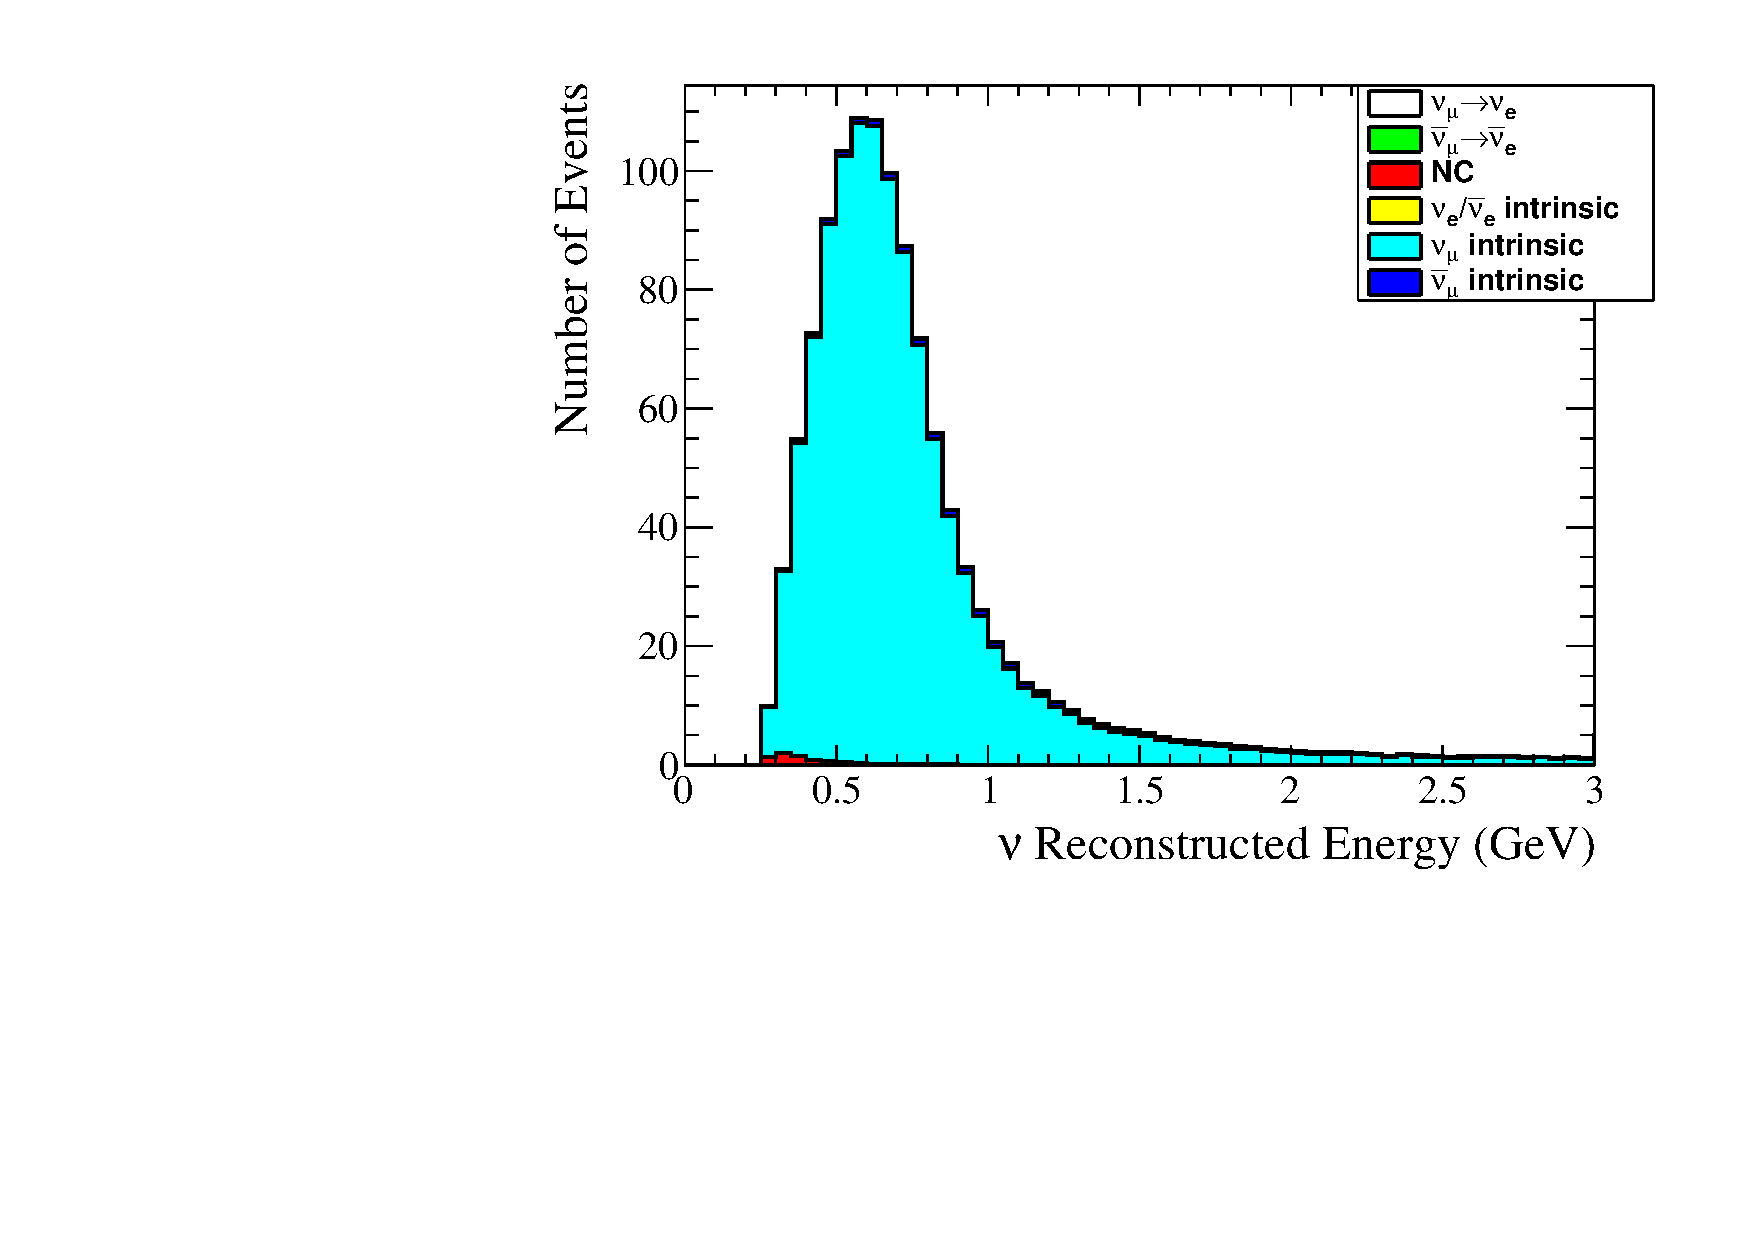
\includegraphics[width=0.9\textwidth]{spectra/spectrum_unosc_1Rmu}
		\caption{Muon-like, neutrino mode}
	\end{subfigure}
	\begin{subfigure}[b]{0.49\textwidth}
		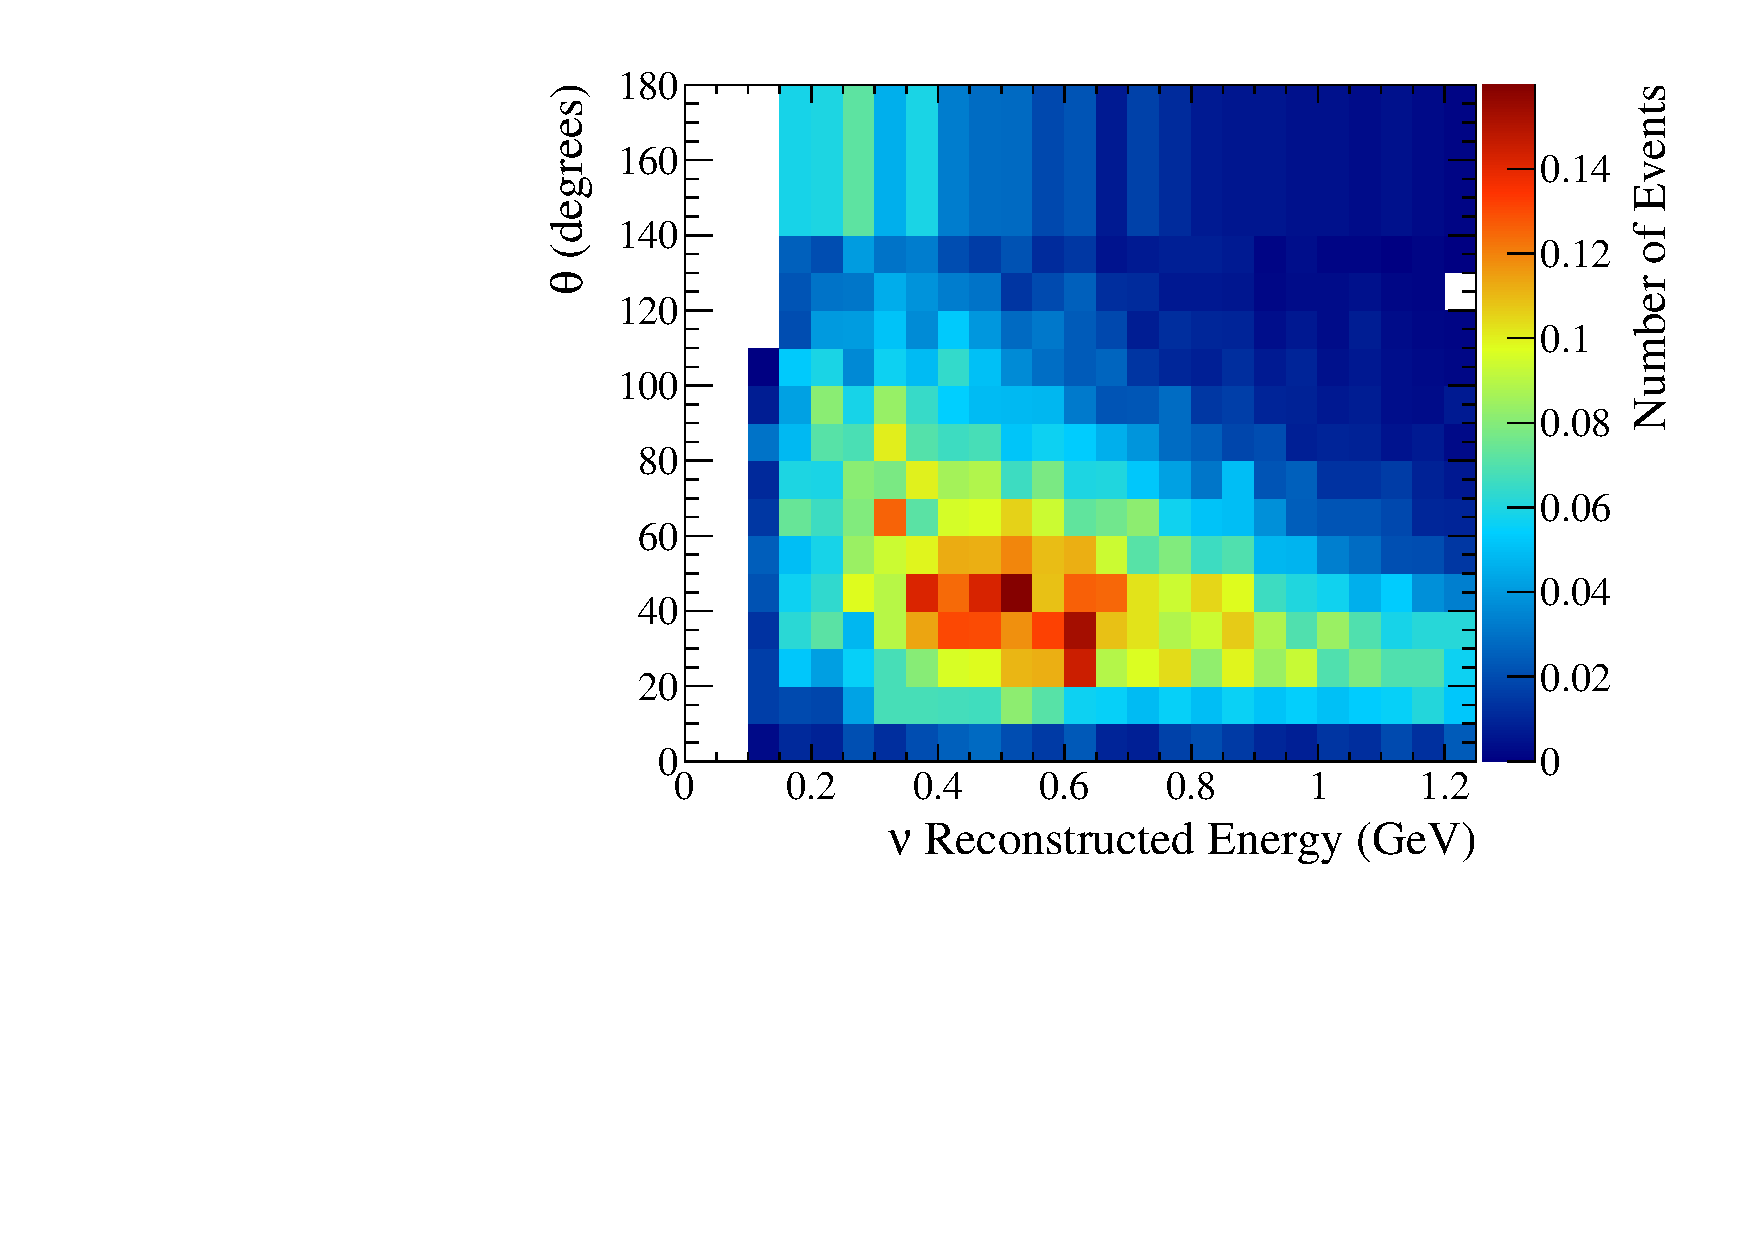
\includegraphics[width=0.9\textwidth]{spectra/spectrum_unosc_1Re}
		\caption{Electron-like, neutrino mode}
	\end{subfigure}
	\begin{subfigure}[b]{0.49\textwidth}
		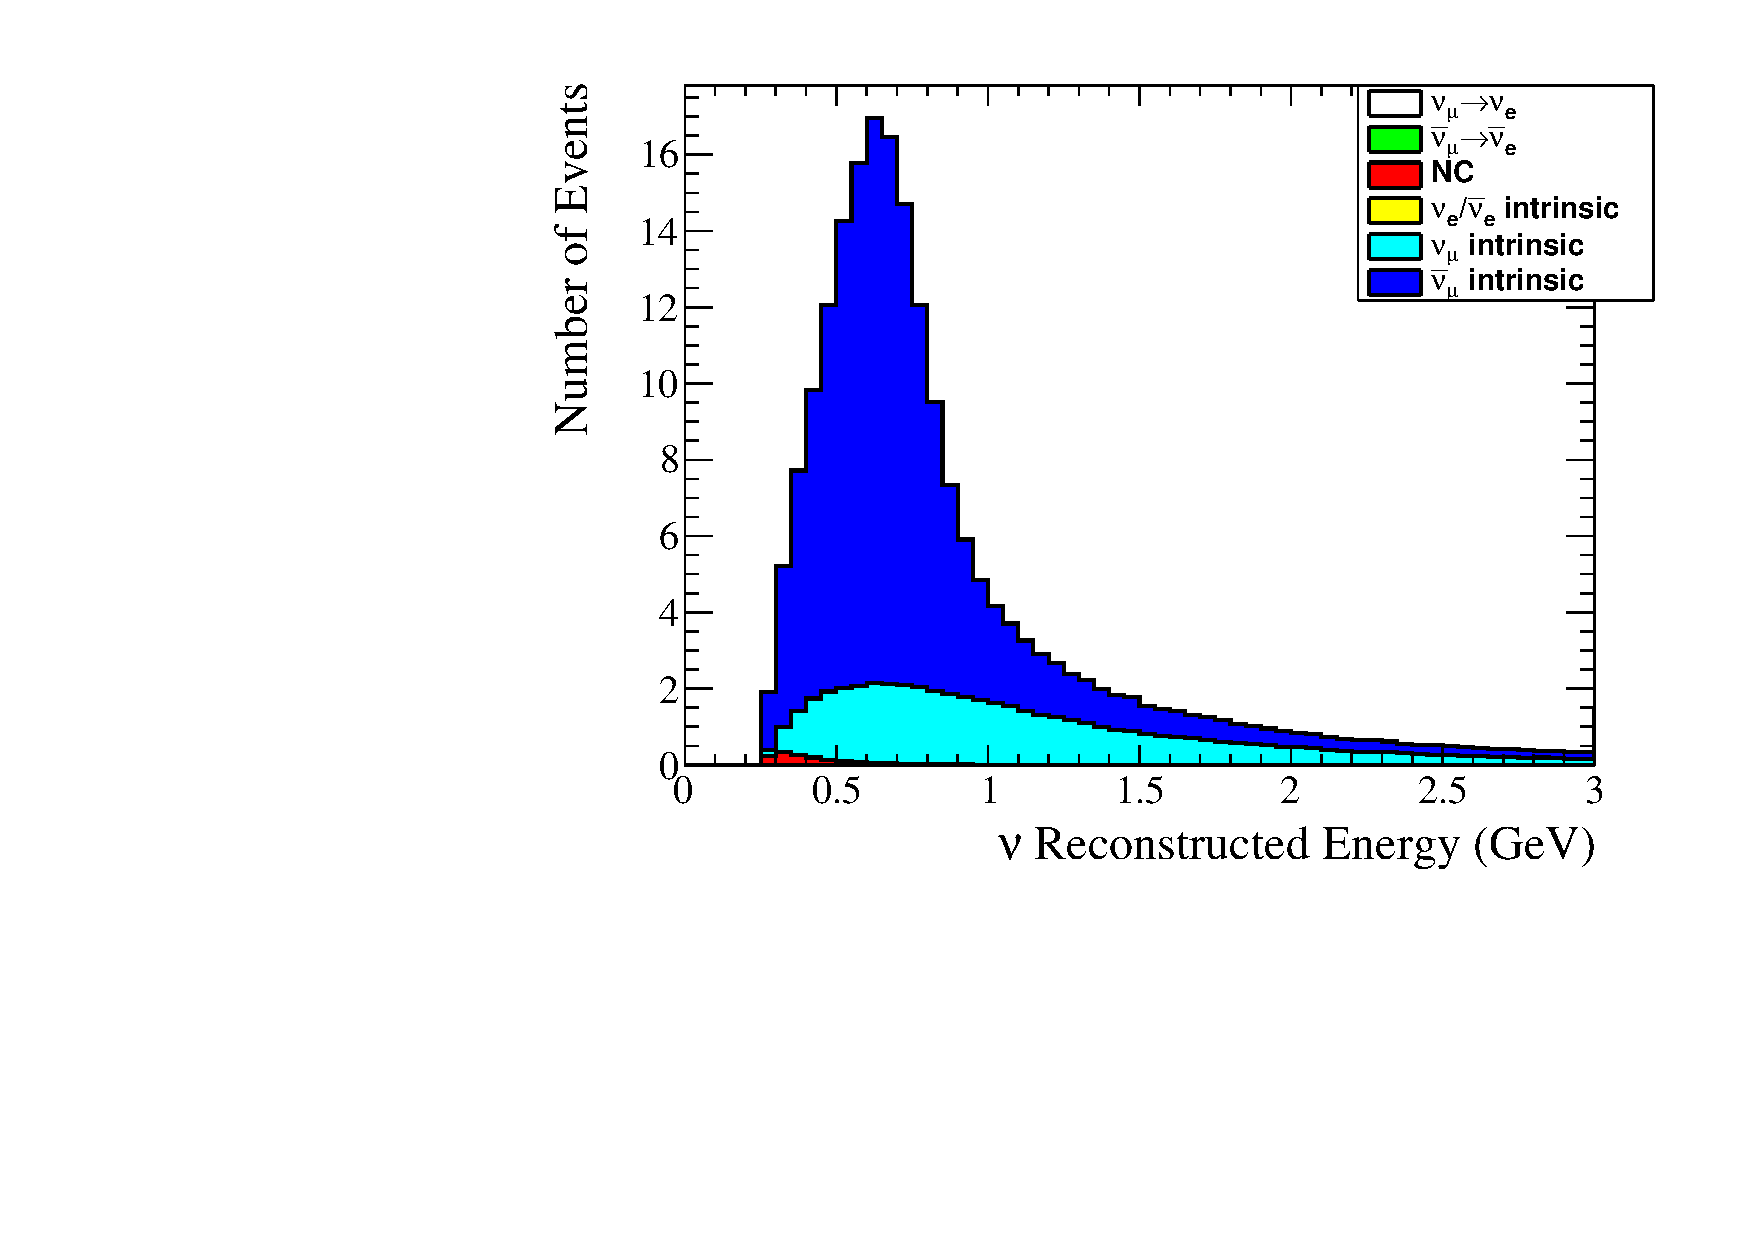
\includegraphics[width=0.9\textwidth]{spectra/spectrum_unosc_RHC1Rmu}
		\caption{Muon-like, antineutrino mode}
	\end{subfigure}
	\begin{subfigure}[b]{0.49\textwidth}
		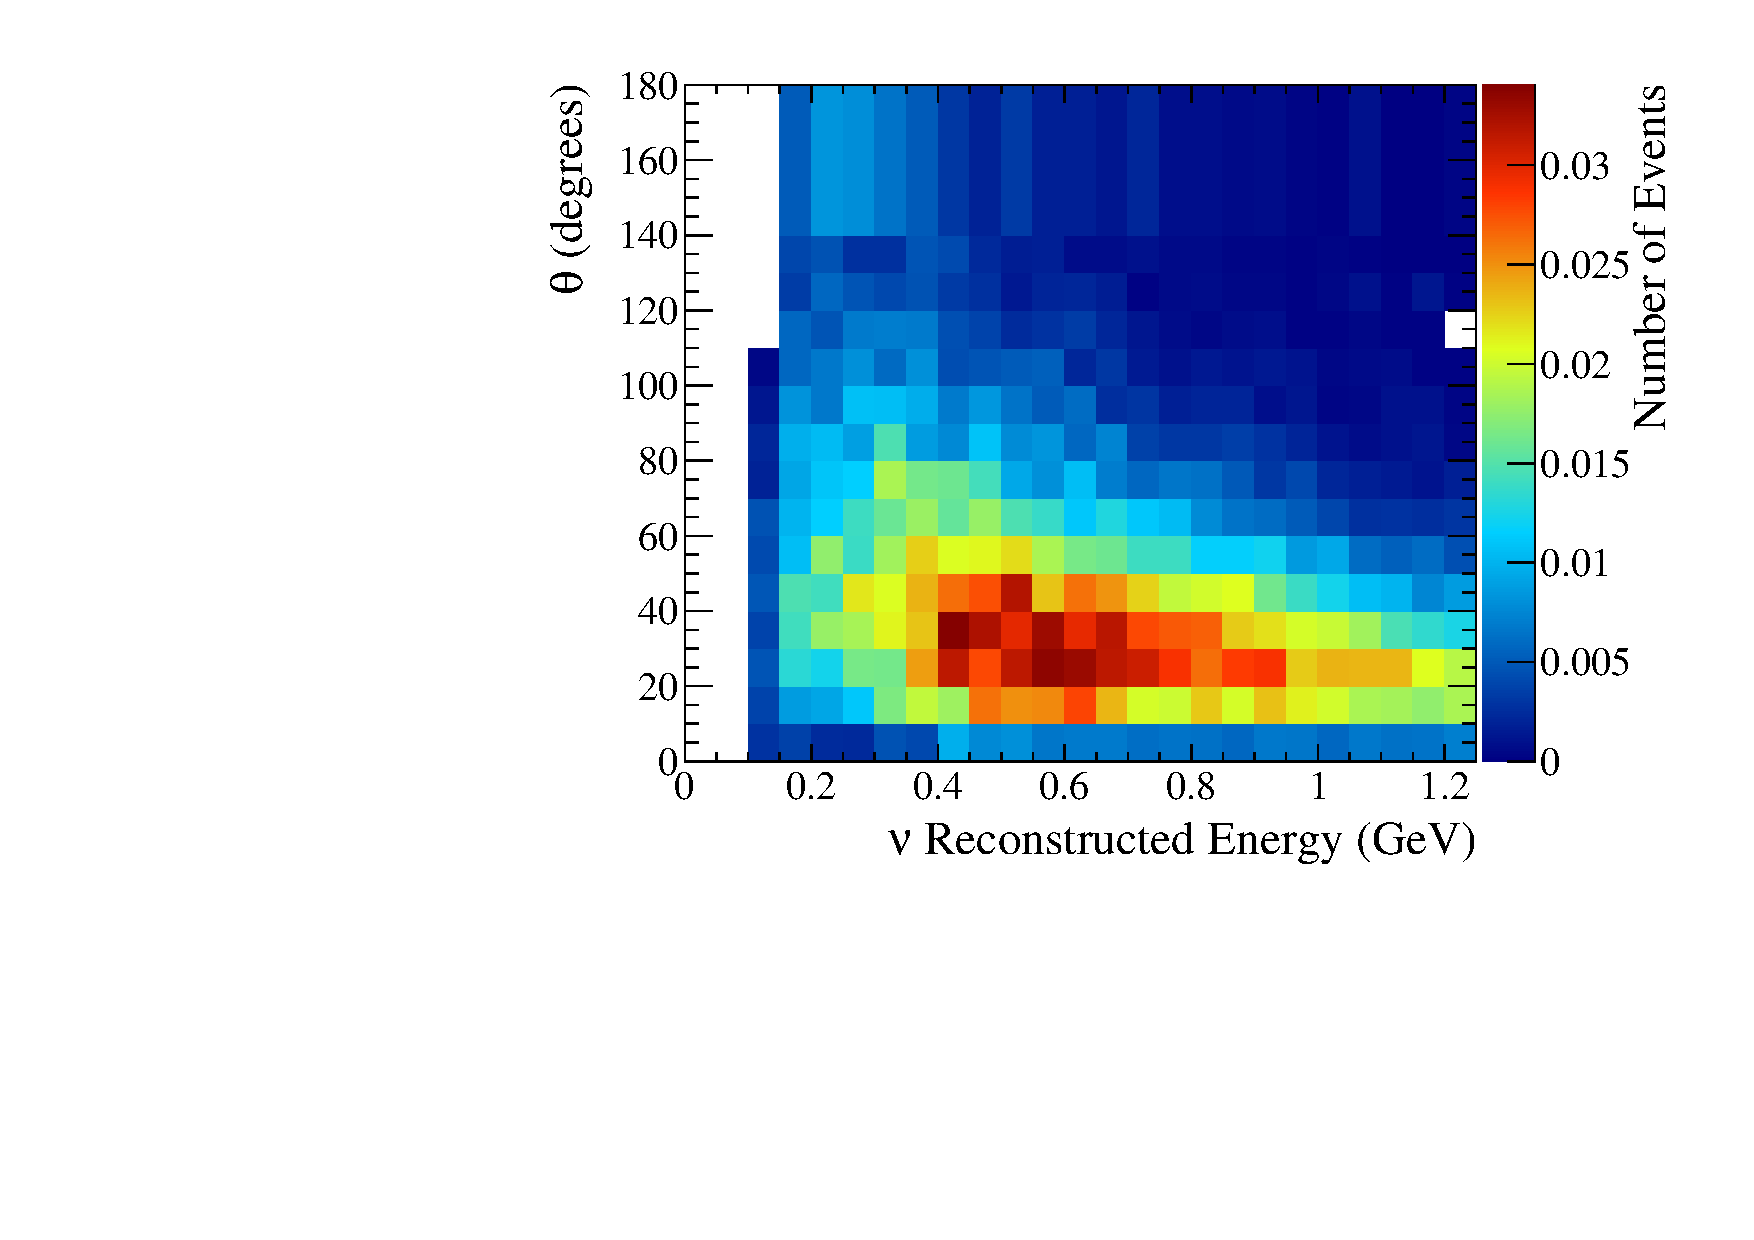
\includegraphics[width=0.9\textwidth]{spectra/spectrum_unosc_RHC1Re}
		\caption{Electron-like antineutrino mode}
	\end{subfigure}
	\begin{subfigure}[b]{0.49\textwidth}
		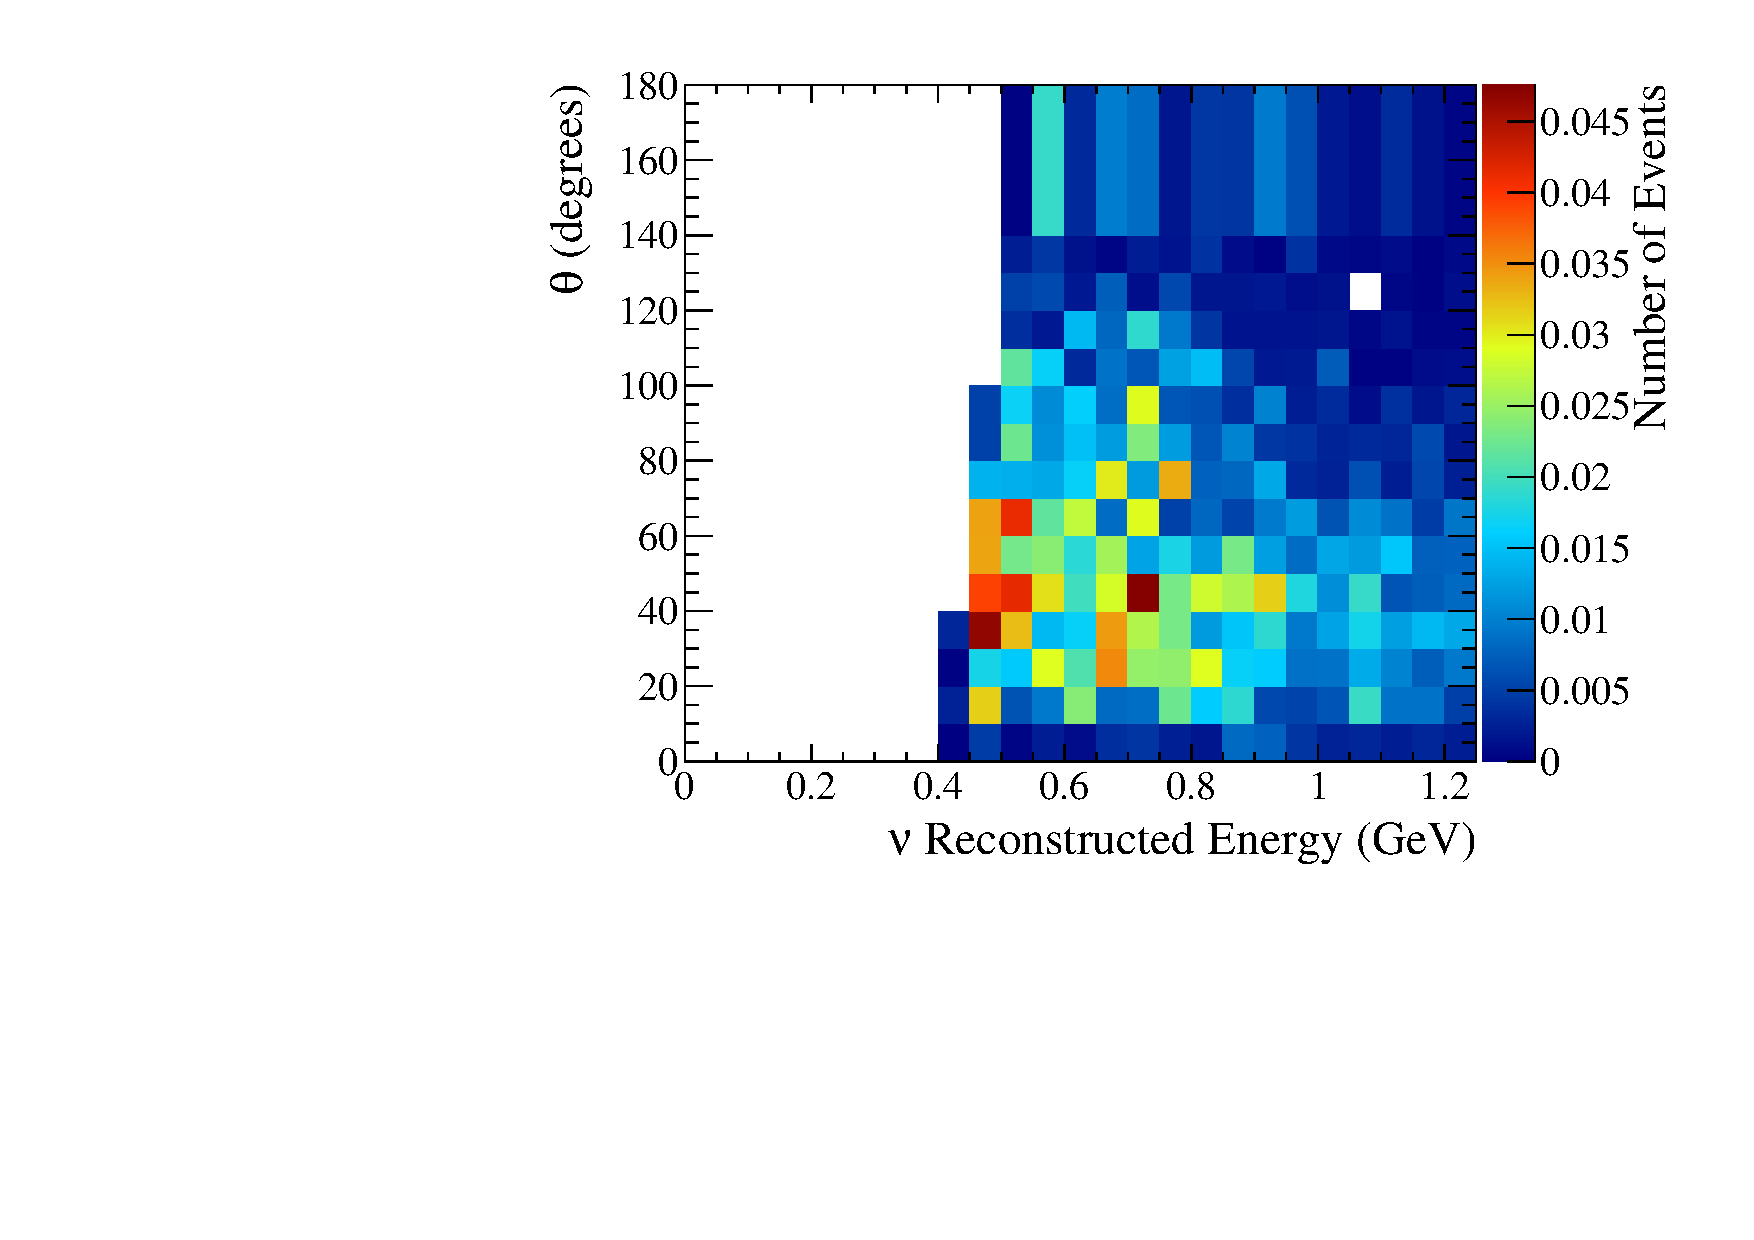
\includegraphics[width=0.9\textwidth]{spectra/spectrum_unosc_MultiRe}
		\caption{\nueCConepi-like, neutrino mode}
	\end{subfigure}
	\caption {
		Predicted unoscillated spectra. $\mu$-like distributions are a function of the reconstructed neutrino energy, while the $e$-like, including \nueCConepi, distributions are functions of both the reconstructed neutrino energy and the reconstructed angle between the outgoing lepton and the neutrino direction. The distributions correspond to the statistics collected in the full \RunPeriod data set. The spectra are generated with the systematic parameters described in \cref{sec:systematics}.
	}
	\label{fig:unosc_spectra_all}
\end{figure*}
\clearpage
\begin{figure*}[htb]
	\center
	\begin{subfigure}[b]{0.49\textwidth}
		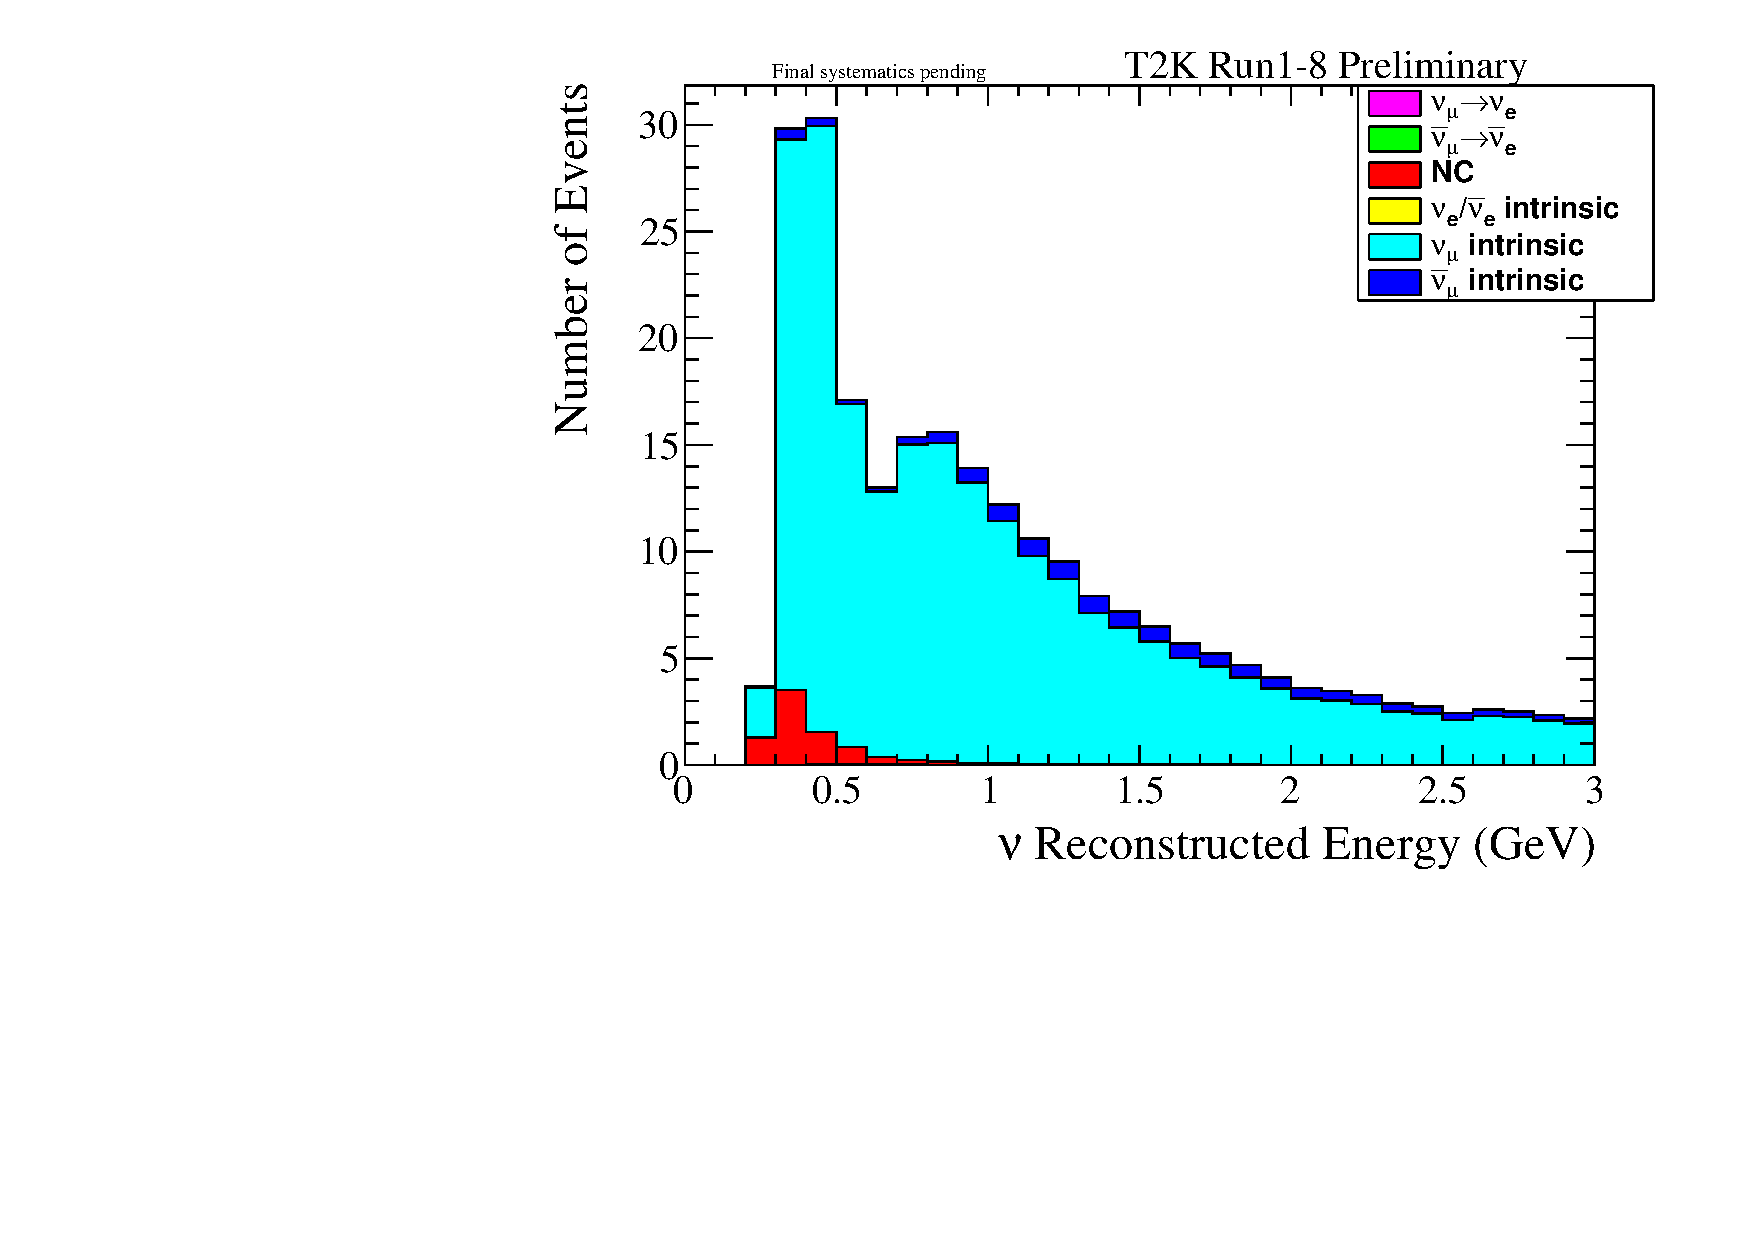
\includegraphics[width=0.9\textwidth]{spectra/spectrum_osc_asimova_1Rmu}
		\caption{Muon-like, neutrino mode}
	\end{subfigure}
	\begin{subfigure}[b]{0.49\textwidth}
		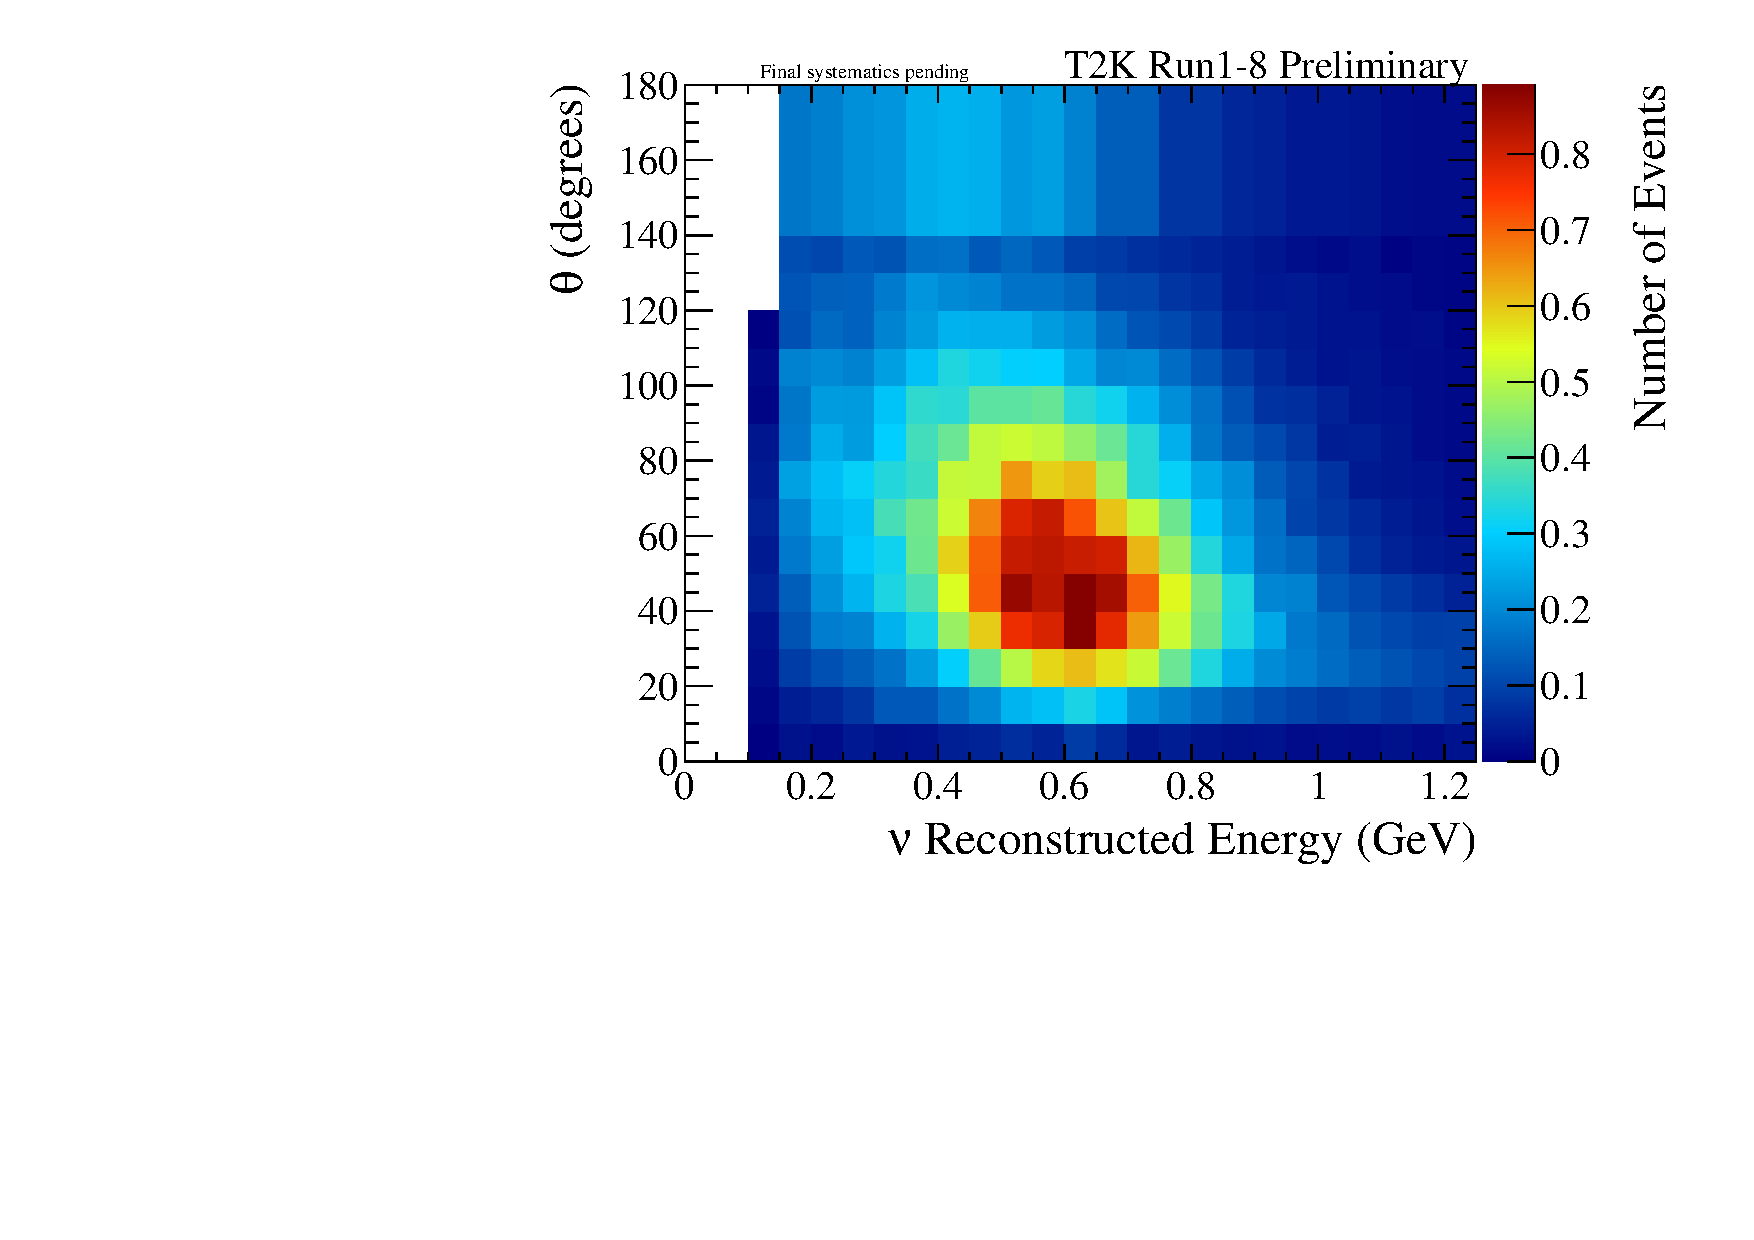
\includegraphics[width=0.9\textwidth]{spectra/spectrum_osc_asimova_1Re}
		\caption{Electron-like, neutrino mode}
	\end{subfigure}
	\begin{subfigure}[b]{0.49\textwidth}
		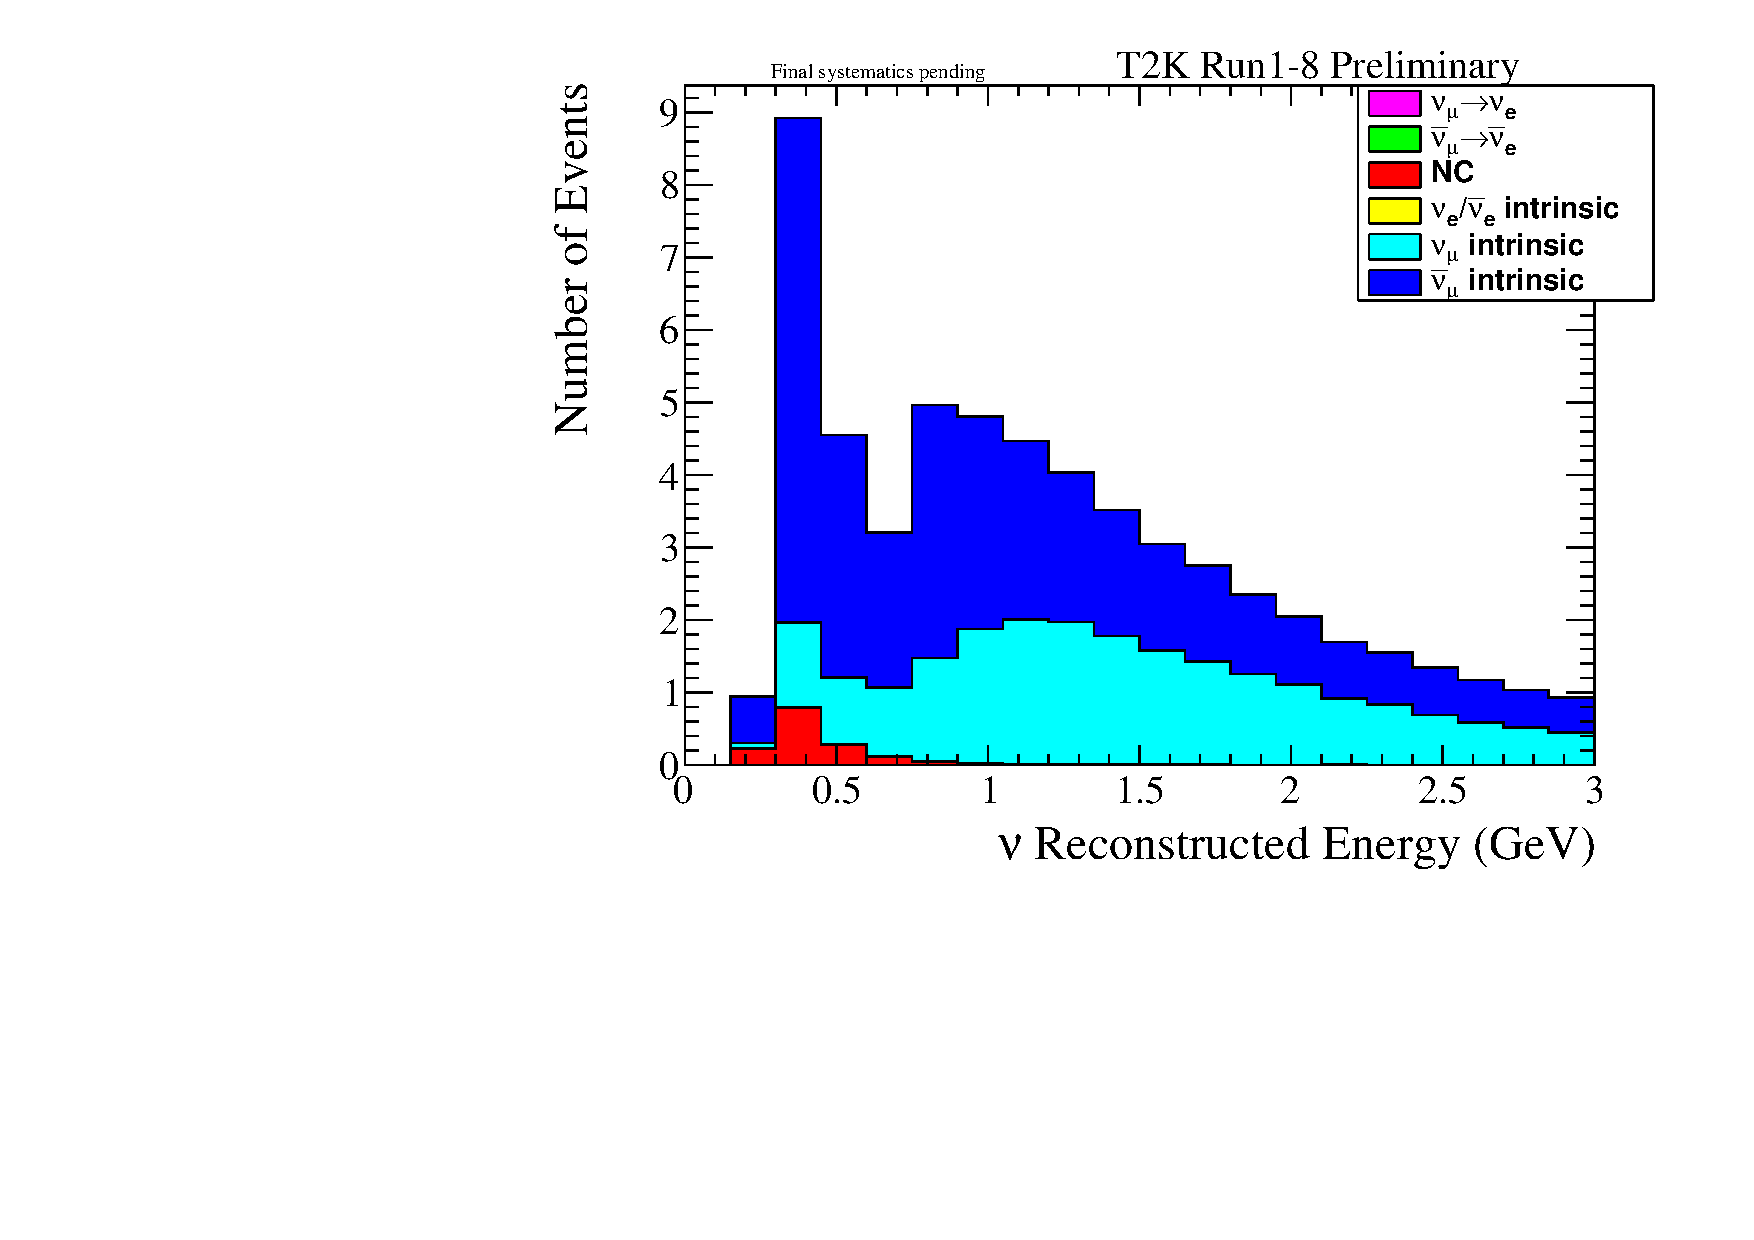
\includegraphics[width=0.9\textwidth]{spectra/spectrum_osc_asimova_RHC1Rmu}
		\caption{Muon-like, antineutrino mode}
	\end{subfigure}
	\begin{subfigure}[b]{0.49\textwidth}
		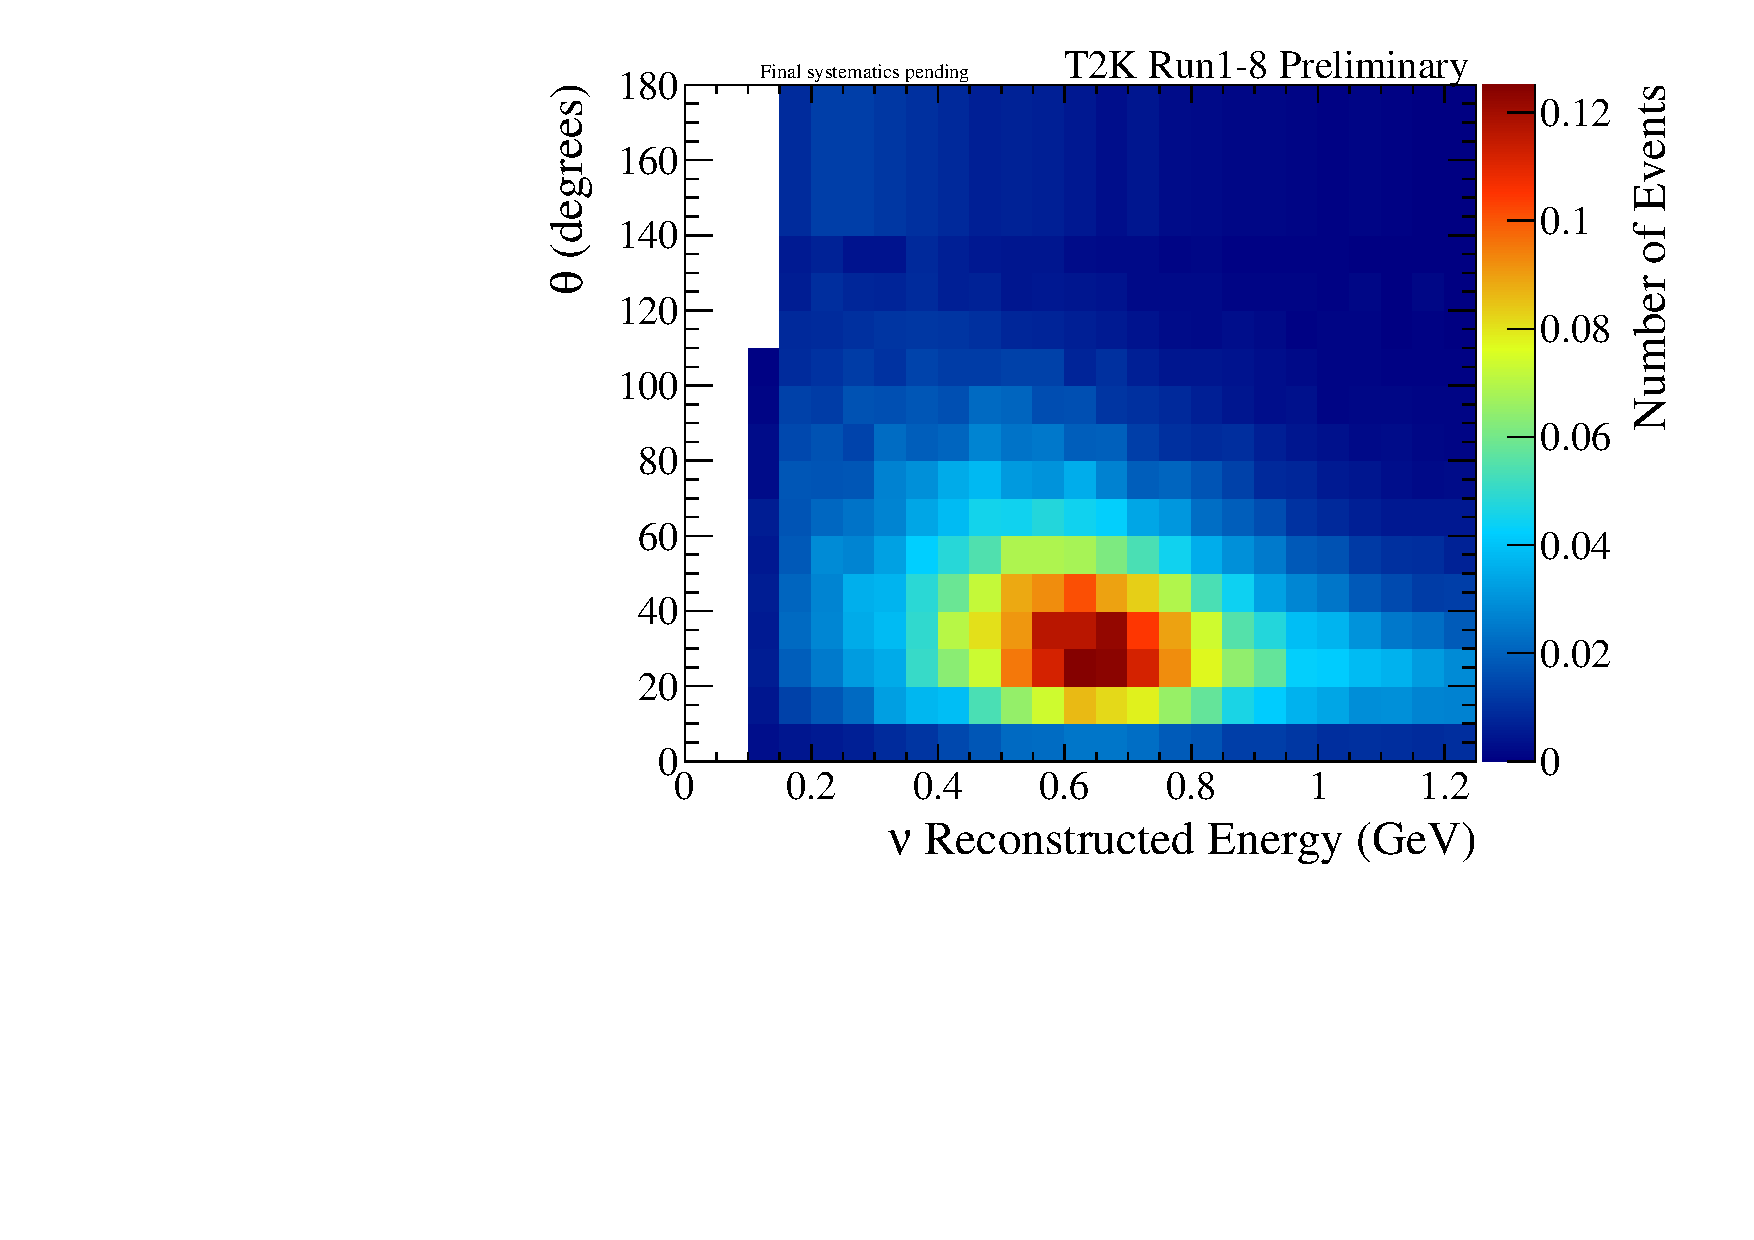
\includegraphics[width=0.9\textwidth]{spectra/spectrum_osc_asimova_RHC1Re}
		\caption{Electron-like antineutrino mode}
	\end{subfigure}
	\begin{subfigure}[b]{0.49\textwidth}
		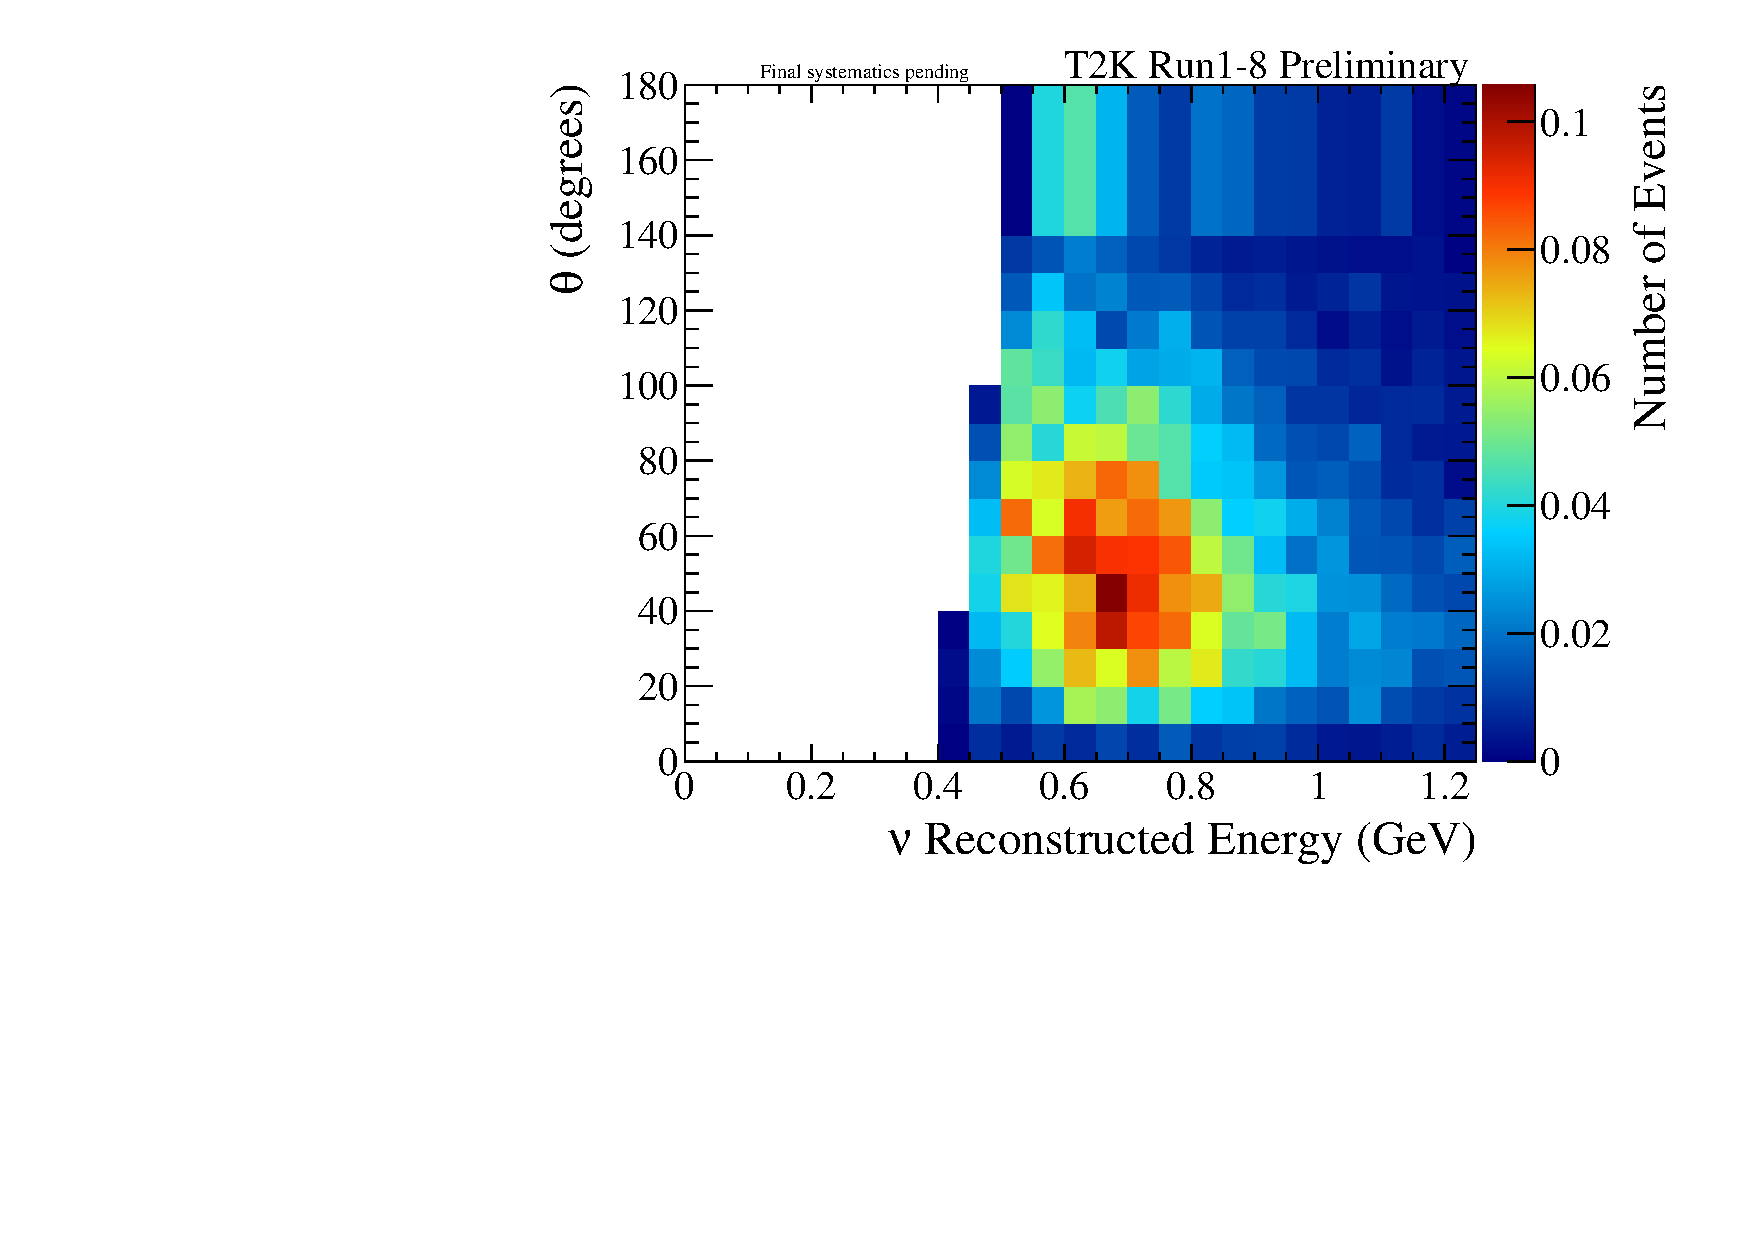
\includegraphics[width=0.9\textwidth]{spectra/spectrum_osc_asimova_MultiRe}
		\caption{\nueCConepi-like, neutrino mode}
	\end{subfigure}
	\caption {
		Predicted Asimov A spectra. $\mu$-like distributions are a function of the reconstructed neutrino energy, while the $e$-like, including \nueCConepi, distributions are functions of both the reconstructed neutrino energy and the reconstructed angle between the outgoing lepton and the neutrino direction. The distributions correspond to the statistics collected in the full \RunPeriod data set. The spectra are generated with the systematic parameters described in \cref{sec:systematics} and the oscillation parameters corresponding to the Asimov data set A shown in \cref{tab:asimov_definition1}.
	}
	\label{fig:asimova_spectra_all}
\end{figure*}
\clearpage

%%% Local Variables:
%%% mode: latex
%%% TeX-master: "../TN327.tex"
%%% End:

\clearpage

\section {Systematic effects in the prediction of the single $\mu$-like ring event energy spectrum}
\label{sec:systematics}

This analysis considers \NSyst{} flux, cross section and Super-K detector systematic parameters plus 7 oscillation parameters, which can be treated as either nuisance ps or as parameters of interest, depending on the analysis that is performed.

\subsection{Flux and cross-section parameters (\NFluxAndXsecSyst{} parameters)}

In this analysis, all the flux and cross-section systematic parameters are included in the ND280 data (BANFF) fit. However, since ND280 is not sensitive to the electron neutrino cross section and the NC1$\gamma$ parameters they remain unconstrained. The parameters fit are 11 $\nu_{\mu}$, 5 $\bar{\nu}_{\mu}$, 7 $\nu_{e}$ and 2 $\bar{\nu}_{e}$ neutrino mode (FHC) flux parameters, 5 $\nu_{\mu}$, 11 $\bar{\nu}_{\mu}$, 2 $\nu_{e}$ and 7 $\bar{\nu}_{e}$ antineutrino mode (RHC) flux parameters and \NXsecSyst{} cross-section parameters. Best-fit values of these parameters and a covariance matrix giving their correlated uncertainties are obtained by the BANFF group from a fit of the $\bar{\nu}_\mu$ and $\nu_\mu$ ND280 samples as described in Ref~\cite{BANFF2017}. A list of the BANFF parameters, their best-fit values and their prefit and postfit errors can be found in \crefrange{tab:sys_flux_fhc_err}{tab:sys_xsec_err}.

\begin{table}
	\begin{tabular} { | c | c | c | c | c |  }
\hline 
Index & Parameter & Description & Best fit & $1\sigma$ pre/postfit\\ 
 & &  &  & fractional error\\
\hline 
0 & $f_{0; t, r}^{banff}$ & FHC $\nu_\mu$ flux normalisation, E = 0.0 - 0.4 GeV & 1.026 & 0.099 / 0.057\\ 
1 & $f_{1; t, r}^{banff}$ & FHC $\nu_\mu$ flux normalisation, E = 0.4 - 0.5 GeV & 1.050 & 0.103 / 0.052\\ 
2 & $f_{2; t, r}^{banff}$ & FHC $\nu_\mu$ flux normalisation, E = 0.5 - 0.6 GeV & 1.032 & 0.096 / 0.045\\ 
3 & $f_{3; t, r}^{banff}$ & FHC $\nu_\mu$ flux normalisation, E = 0.6 - 0.7 GeV & 0.991 & 0.087 / 0.042\\ 
4 & $f_{4; t, r}^{banff}$ & FHC $\nu_\mu$ flux normalisation, E = 0.7 - 1.0 GeV & 0.943 & 0.113 / 0.054\\ 
5 & $f_{5; t, r}^{banff}$ & FHC $\nu_\mu$ flux normalisation, E = 1.0 - 1.5 GeV & 0.963 & 0.092 / 0.049\\ 
6 & $f_{6; t, r}^{banff}$ & FHC $\nu_\mu$ flux normalisation, E = 1.5 - 2.5 GeV & 1.030 & 0.070 / 0.042\\ 
7 & $f_{7; t, r}^{banff}$ & FHC $\nu_\mu$ flux normalisation, E = 2.5 - 3.5 GeV & 1.047 & 0.074 / 0.044\\ 
8 & $f_{8; t, r}^{banff}$ & FHC $\nu_\mu$ flux normalisation, E = 3.5 - 5.0 GeV & 1.038 & 0.087 / 0.041\\ 
9 & $f_{9; t, r}^{banff}$ & FHC $\nu_\mu$ flux normalisation, E = 5.0 - 7.0 GeV & 1.003 & 0.098 / 0.040\\ 
10 & $f_{10; t, r}^{banff}$ & FHC $\nu_\mu$ flux normalisation, E = 7.0 - 30.0 GeV & 0.991 & 0.114 / 0.048\\ 
11 & $f_{11; t, r}^{banff}$ & FHC $\bar{\nu_\mu}$ flux normalisation, E = 0.0 - 0.7 GeV & 0.989 & 0.103 / 0.074\\ 
12 & $f_{12; t, r}^{banff}$ & FHC $\bar{\nu_\mu}$ flux normalisation, E = 0.7 - 1.0 GeV & 0.986 & 0.079 / 0.048\\ 
13 & $f_{13; t, r}^{banff}$ & FHC $\bar{\nu_\mu}$ flux normalisation, E = 1.0 - 1.5 GeV & 0.996 & 0.084 / 0.057\\ 
14 & $f_{14; t, r}^{banff}$ & FHC $\bar{\nu_\mu}$ flux normalisation, E = 1.5 - 2.5 GeV & 1.042 & 0.086 / 0.062\\ 
15 & $f_{15; t, r}^{banff}$ & FHC $\bar{\nu_\mu}$ flux normalisation, E = 2.5 - 30.0 GeV & 1.104 & 0.086 / 0.065\\ 
16 & $f_{16; t, r}^{banff}$ & FHC $\nu_e$ flux normalisation, E = 0.0 - 0.5 GeV & 1.030 & 0.090 / 0.046\\ 
17 & $f_{17; t, r}^{banff}$ & FHC $\nu_e$ flux normalisation, E = 0.5 - 0.7 GeV & 1.031 & 0.090 / 0.042\\ 
18 & $f_{18; t, r}^{banff}$ & FHC $\nu_e$ flux normalisation, E = 0.7 - 0.8 GeV & 1.029 & 0.086 / 0.041\\ 
19 & $f_{19; t, r}^{banff}$ & FHC $\nu_e$ flux normalisation, E = 0.8 - 1.5 GeV & 1.017 & 0.081 / 0.039\\ 
20 & $f_{20; t, r}^{banff}$ & FHC $\nu_e$ flux normalisation, E = 1.5 - 2.5 GeV & 1.034 & 0.079 / 0.040\\ 
21 & $f_{21; t, r}^{banff}$ & FHC $\nu_e$ flux normalisation, E = 2.5 - 4.0 GeV & 1.036 & 0.084 / 0.041\\ 
22 & $f_{22; t, r}^{banff}$ & FHC $\nu_e$ flux normalisation, E = 4.0 - 30.0 GeV & 1.050 & 0.094 / 0.059\\ 
23 & $f_{23; t, r}^{banff}$ & FHC $\bar{\nu_e}$ flux normalisation, E = 0.0 - 2.5 GeV & 1.050 & 0.074 / 0.054\\ 
24 & $f_{24; t, r}^{banff}$ & FHC $\bar{\nu_e}$ flux normalisation, E = 2.5 - 30.0 GeV & 1.093 & 0.128 / 0.114\\ 

\hline

\end{tabular}
	\caption{Summary of neutrino mode flux systematics included in the VALOR joint fit analysis. A description of how the BANFF fit constrained these systematics can be found in \cite{BANFF2017}.}
	\label{tab:sys_flux_fhc_err}
\end{table}

\begin{table}
	\begin{tabular} { | c | c | c | c | c |  }
\hline 
Index & Parameter & Description & Best fit & $1\sigma$ pre/postfit\\ 
 & &  &  & fractional error\\
\hline 
25 & $f_{0; t, r}^{banff} RHC$ & RHC $\nu_\mu$ flux normalisation, E = 0.0 - 0.7 GeV & 0.993 & 0.094 / 0.066\\ 
26 & $f_{1; t, r}^{banff} RHC$ & RHC $\nu_\mu$ flux normalisation, E = 0.7 - 1.0 GeV & 1.003 & 0.079 / 0.049\\ 
27 & $f_{2; t, r}^{banff} RHC$ & RHC $\nu_\mu$ flux normalisation, E = 1.0 - 1.5 GeV & 1.018 & 0.077 / 0.045\\ 
28 & $f_{3; t, r}^{banff} RHC$ & RHC $\nu_\mu$ flux normalisation, E = 1.5 - 2.5 GeV & 1.061 & 0.081 / 0.049\\ 
29 & $f_{4; t, r}^{banff} RHC$ & RHC $\nu_\mu$ flux normalisation, E = 2.5 - 30.0 GeV & 1.051 & 0.080 / 0.043\\ 
30 & $f_{5; t, r}^{banff} RHC$ & RHC $\bar{\nu_\mu}$ flux normalisation, E = 0.0 - 0.4 GeV & 1.012 & 0.104 / 0.065\\ 
31 & $f_{6; t, r}^{banff} RHC$ & RHC $\bar{\nu_\mu}$ flux normalisation, E = 0.4 - 0.5 GeV & 1.028 & 0.102 / 0.052\\ 
32 & $f_{7; t, r}^{banff} RHC$ & RHC $\bar{\nu_\mu}$ flux normalisation, E = 0.5 - 0.6 GeV & 1.008 & 0.096 / 0.045\\ 
33 & $f_{8; t, r}^{banff} RHC$ & RHC $\bar{\nu_\mu}$ flux normalisation, E = 0.6 - 0.7 GeV & 0.988 & 0.085 / 0.041\\ 
34 & $f_{9; t, r}^{banff} RHC$ & RHC $\bar{\nu_\mu}$ flux normalisation, E = 0.7 - 1.0 GeV & 0.986 & 0.125 / 0.052\\ 
35 & $f_{10; t, r}^{banff} RHC$ & RHC $\bar{\nu_\mu}$ flux normalisation, E = 1.0 - 1.5 GeV & 0.997 & 0.105 / 0.047\\ 
36 & $f_{11; t, r}^{banff} RHC$ & RHC $\bar{\nu_\mu}$ flux normalisation, E = 1.5 - 2.5 GeV & 1.036 & 0.080 / 0.042\\ 
37 & $f_{12; t, r}^{banff} RHC$ & RHC $\bar{\nu_\mu}$ flux normalisation, E = 2.5 - 3.5 GeV & 1.063 & 0.074 / 0.046\\ 
38 & $f_{13; t, r}^{banff} RHC$ & RHC $\bar{\nu_\mu}$ flux normalisation, E = 3.5 - 5.0 GeV & 1.069 & 0.094 / 0.063\\ 
39 & $f_{14; t, r}^{banff} RHC$ & RHC $\bar{\nu_\mu}$ flux normalisation, E = 5.0 - 7.0 GeV & 1.044 & 0.093 / 0.056\\ 
40 & $f_{15; t, r}^{banff} RHC$ & RHC $\bar{\nu_\mu}$ flux normalisation, E = 7.0 - 30.0 GeV & 1.007 & 0.130 / 0.093\\ 
41 & $f_{16; t, r}^{banff} RHC$ & RHC $\nu_e$ flux normalisation, E = 0.0 - 2.5 GeV & 1.050 & 0.069 / 0.047\\ 
42 & $f_{17; t, r}^{banff} RHC$ & RHC $\nu_e$ flux normalisation, E = 2.5 - 30.0 GeV & 1.048 & 0.085 / 0.065\\ 
43 & $f_{18; t, r}^{banff} RHC$ & RHC $\bar{\nu_e}$ flux normalisation, E = 0.0 - 0.5 GeV & 1.018 & 0.095 / 0.051\\ 
44 & $f_{19; t, r}^{banff} RHC$ & RHC $\bar{\nu_e}$ flux normalisation, E = 0.5 - 0.7 GeV & 1.018 & 0.091 / 0.043\\ 
45 & $f_{20; t, r}^{banff} RHC$ & RHC $\bar{\nu_e}$ flux normalisation, E = 0.7 - 0.8 GeV & 1.016 & 0.091 / 0.044\\ 
46 & $f_{21; t, r}^{banff} RHC$ & RHC $\bar{\nu_e}$ flux normalisation, E = 0.8 - 1.5 GeV & 1.018 & 0.084 / 0.040\\ 
47 & $f_{22; t, r}^{banff} RHC$ & RHC $\bar{\nu_e}$ flux normalisation, E = 1.5 - 2.5 GeV & 1.043 & 0.080 / 0.051\\ 
48 & $f_{23; t, r}^{banff} RHC$ & RHC $\bar{\nu_e}$ flux normalisation, E = 2.5 - 4.0 GeV & 1.046 & 0.089 / 0.064\\ 
49 & $f_{24; t, r}^{banff} RHC$ & RHC $\bar{\nu_e}$ flux normalisation, E = 4.0 - 30.0 GeV & 1.083 & 0.156 / 0.133\\ 

\hline

\end{tabular}
	\caption{Summary of antineutrino mode flux systematics included in the VALOR joint fit analysis. A description of how the BANFF fit constrained these systematics can be found in \cite{BANFF2017}.}
	\label{tab:sys_flux_rhc_err}
\end{table}


\begin{table}
	\begin{adjustbox}{width=\textwidth, totalheight=\textheight, keepaspectratio}
		\begin{tabular} { | c | c | c | c | c |  }
\hline 
Index & Parameter & Description & Best fit & $1\sigma$ pre/postfit\\ 
 & &  &  & fractional error\\
\hline 
50 & $f_{Norm_{2p2h}}^{banff}$ & Two particle two hole normalisation for $^{16}$O & 1.426 & 1.000 / 0.182\\ 
51 & $f_{C^{A}_{5}}^{banff}$ & C$^{A}_{5}$ nucleon to $\Delta$ transition axial form factor & 0.977 & 0.149 / 0.059\\ 
52 & $f_{Bg_{RES}}^{banff}$ & Scale of isospin 1/2 nonresonant background & 0.979 & 0.308 / 0.190\\ 
53 & $f_{M_A^{QE}}^{banff}$ & CCQE axial-mass scaling factor & 0.903 & 0.025 / 0.057\\ 
54 & $f_{M_A^{RES}}^{banff}$ & Resonance-production axial-mass scaling factor & 0.822 & 0.158 / 0.045\\ 
55 & $f_{SCCA}^{banff}$ & BANFF; Second current class axial & 1.000 & - / -\\ 
56 & $f_{SCCV}^{banff}$ & BANFF; Second current class vector & 1.000 & - / -\\ 
57 & $f_{p_{f}}^{banff}$ & Fermi momentum for $^{16}$O & 0.916 & 0.058 / 0.072\\ 
58 & $f_{Shape_{CCoth}}^{banff}$ & CC other shape & 0.519 & 0.400 / 0.187\\ 
59 & $f_{Norm_{CCcoh}}^{banff}$ & CC coherent for $^{16}$O normalisation & 0.906 & 0.300 / 0.275\\ 
60 & $f_{Norm_{NCcoh}}^{banff}$ & NC coherent normalisation & 0.939 & 0.300 / 0.297\\ 
61 & $f_{Norm_{NCother}}^{banff}$ & NC other normalisation & 1.000 & - / 0.300\\ 
62 & $f_{Norm_{\nu_e \rightarrow \nu_\mu}}^{banff}$ & CC $\nu_{e}$ normalisation & 1.000 & - / 0.028\\ 
63 & $f_{Norm_{NC1\gamma}}^{banff}$ & NC 1$\gamma$ normalisation & 1.000 & - / 1.000\\ 
64 & $f_{Norm_{\bar{\nu}_e \rightarrow \bar{\nu}_{\mu}}}^{banff}$ & CC $\bar{\nu}_{e}$ normalisation & 1.000 & - / 0.028\\ 
65 & $f_{Norm_{2p2hBar}}^{banff}$ & Antineutrino two particle two hole normalisation for $^{16}$O & 0.552 & 1.000 / 0.201\\ 
66 & $f_{Shape_{BeRPA_{A}}}^{banff}$ & Bernstein Polynomial coefficient A & 0.663 & 0.118 / 0.056\\ 
67 & $f_{Shape_{BeRPA_{B}}}^{banff}$ & Bernstein Polynomial coefficient B & 1.647 & 0.210 / 0.117\\ 
68 & $f_{Shape_{BeRPA_{D}}}^{banff}$ & Bernstein Polynomial coefficient D & 0.988 & 0.170 / 0.128\\ 
69 & $f_{Shape_{BeRPA_{E}}}^{banff}$ & Bernstein Polynomial coefficient E & 0.876 & 0.352 / 0.355\\ 
70 & $f_{Shape_{BeRPA_{U}}}^{banff}$ & Bernstein Polynomial coefficient U & 1.200 & 0.100 / 0.100\\ 
71 & $f_{Shape_{2p2h\nu}}^{banff}$ & Neutrino two particle two hole $^{16}$O shape & 0.997 & 3.000 / 0.338\\ 
72 & $f_{Norm_{2p2h C to O}}^{banff}$ & Two particle two hole $^{12}$C to $^{16}$O normalisation & 0.940 & 0.200 / 0.161\\ 

\hline

\end{tabular}
	\end{adjustbox}
	\caption{Summary of cross section systematics included in the VALOR joint fit analysis. Parameters with no prefit error were unconstrained. A description of how the BANFF fit constrained these systematics can be found in \cite{BANFF2017}.}
	\label{tab:sys_xsec_err}
\end{table}

%Previously the next reference was banff-weights, might want to include more detail
The best-fit values are used to reweight the templates as described in \Cref{app:details}, and the postfit errors in the covariance matrix are used as prior uncertainties in this analysis. All the cross section parameters set to 1 correspond to the NEUT nominal value, except ``CC other shape'' and ``2p2h shape O'', for which the NEUT nominal value is 0.  For all the normalisation parameters, 1 is the nominal pre-BANFF fit value.

The effects of these correlated uncertainties (see \cref{fig:xsec_corr}) are evaluated using the Cholesky method, that allows throws of the systematic parameters according to their multivariate distribution taking into account existing correlations.

\begin{figure*}[htb]
	\center
	\begin{subfigure}[b]{0.49\textwidth}
		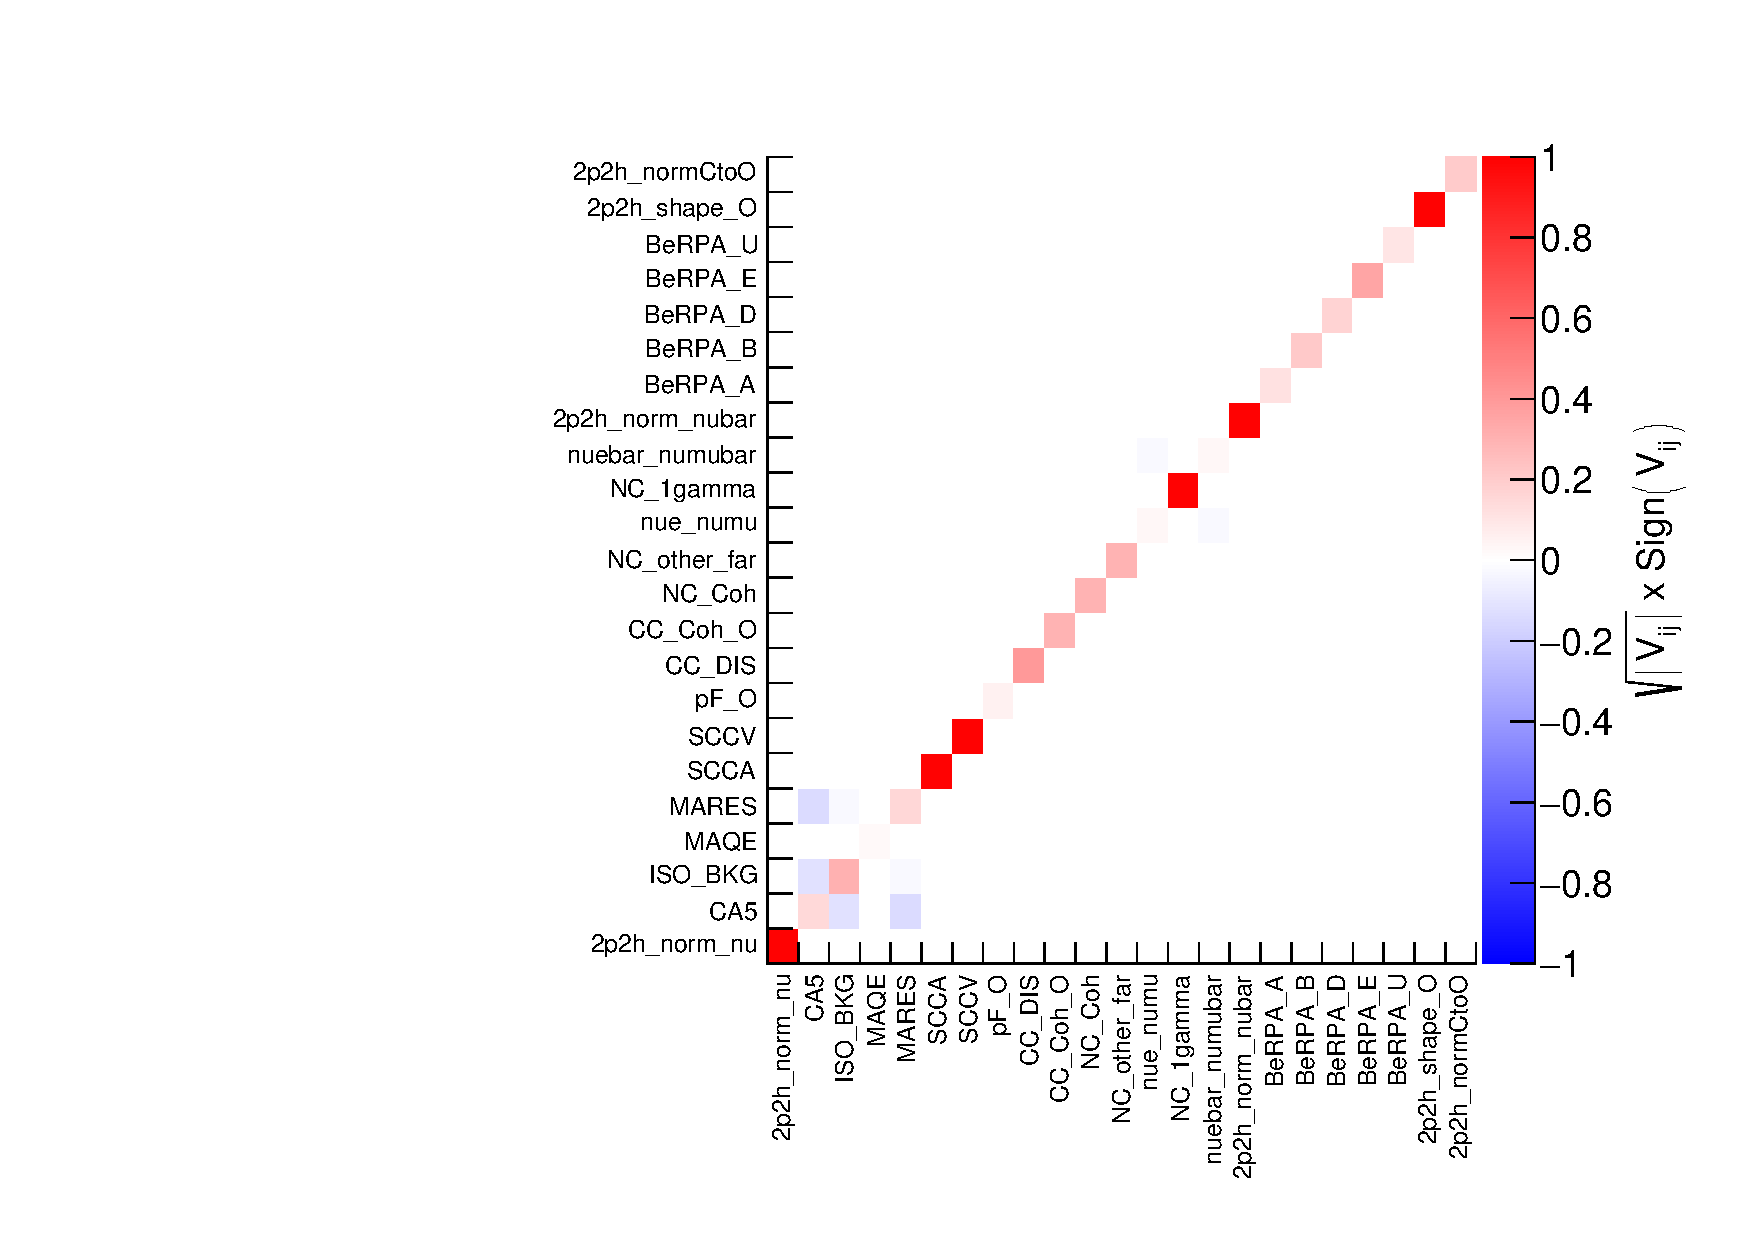
\includegraphics[angle=-90,width=0.9\textwidth]{systematics/banff_xsec_prefit}
	\end{subfigure}
	\begin{subfigure}[b]{0.49\textwidth}
		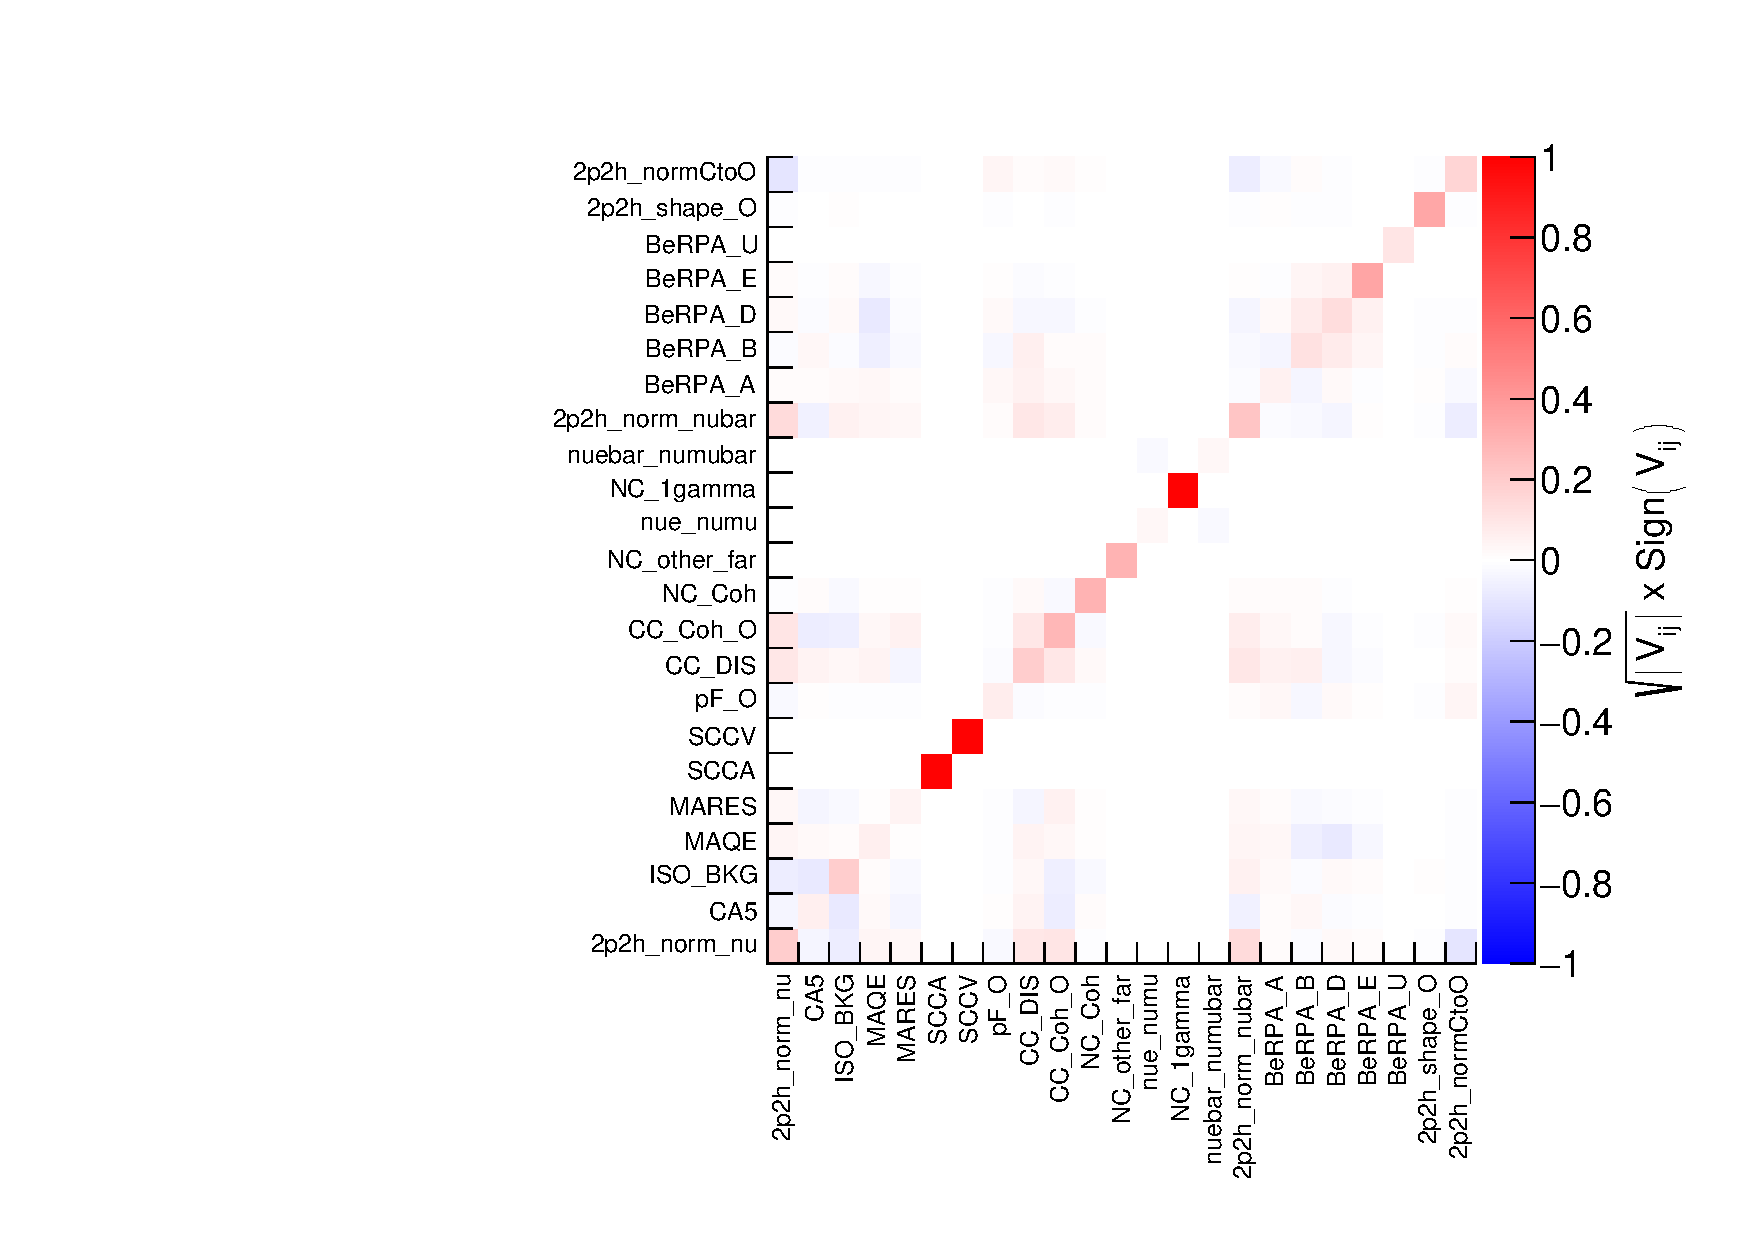
\includegraphics[angle=-90,width=0.9\textwidth]{systematics/banff_xsec_postfit}
	\end{subfigure}
	\caption{The pre-BANFF (left) and post-BANFF (right) cross-section covariance matrix, with the values shown as the sign of the element times the square root of the absolute value of the element.}
\label{fig:xsec_corr}
\end{figure*}

Many of the cross-section parameters are the same as those used in the previous analysis \cite{OurRun17cCC1piJointAnalysis3Flavour}. However, the binding energy for $^{16}$O is no longer included in this analysis and a number of new parameters have been included, see \cref{sec:systematics:2p2h_berpa}. Five of these new parameters (2p2h, BeRPA A, B, D and E) are implemented using cubic splines, details for which can be found in \cite{OurRun17cCC1piJointAnalysis3Flavour}, while one of the new parameters (BeRPA U) is fixed in the analysis.

\subsubsection{Neutrino-nucleus interaction uncertainties}
\label{sec:systematics:2p2h_berpa}
Overall normalisation uncertainties for 2p2h interactions were included in previous analyses, but this analysis includes a 2p2h shape uncertainty (using best-fit value and errors from the BANFF fit) to describe the uncertainty in the cross-section strength between Delta-like, non-Delta-like and interference terms of the 2p2h model, determined by redistributing the cross-section strength of these terms subject to (approximately) maintaining the total 2p2h event rate (see Section 2 of \cite{NewXsecImplementation}). In terms of energy transfer (q0) and three-momentum transfer (q3) kinematics, the distribution of events in this space for neutrino and antineutrino interactions on oxygen are shown in \cref{fig:2p2h_neutrino,fig:2p2h_antineutrino} respectively (see Section 2 of \cite{NewXsecImplementation}).

\begin{figure}
	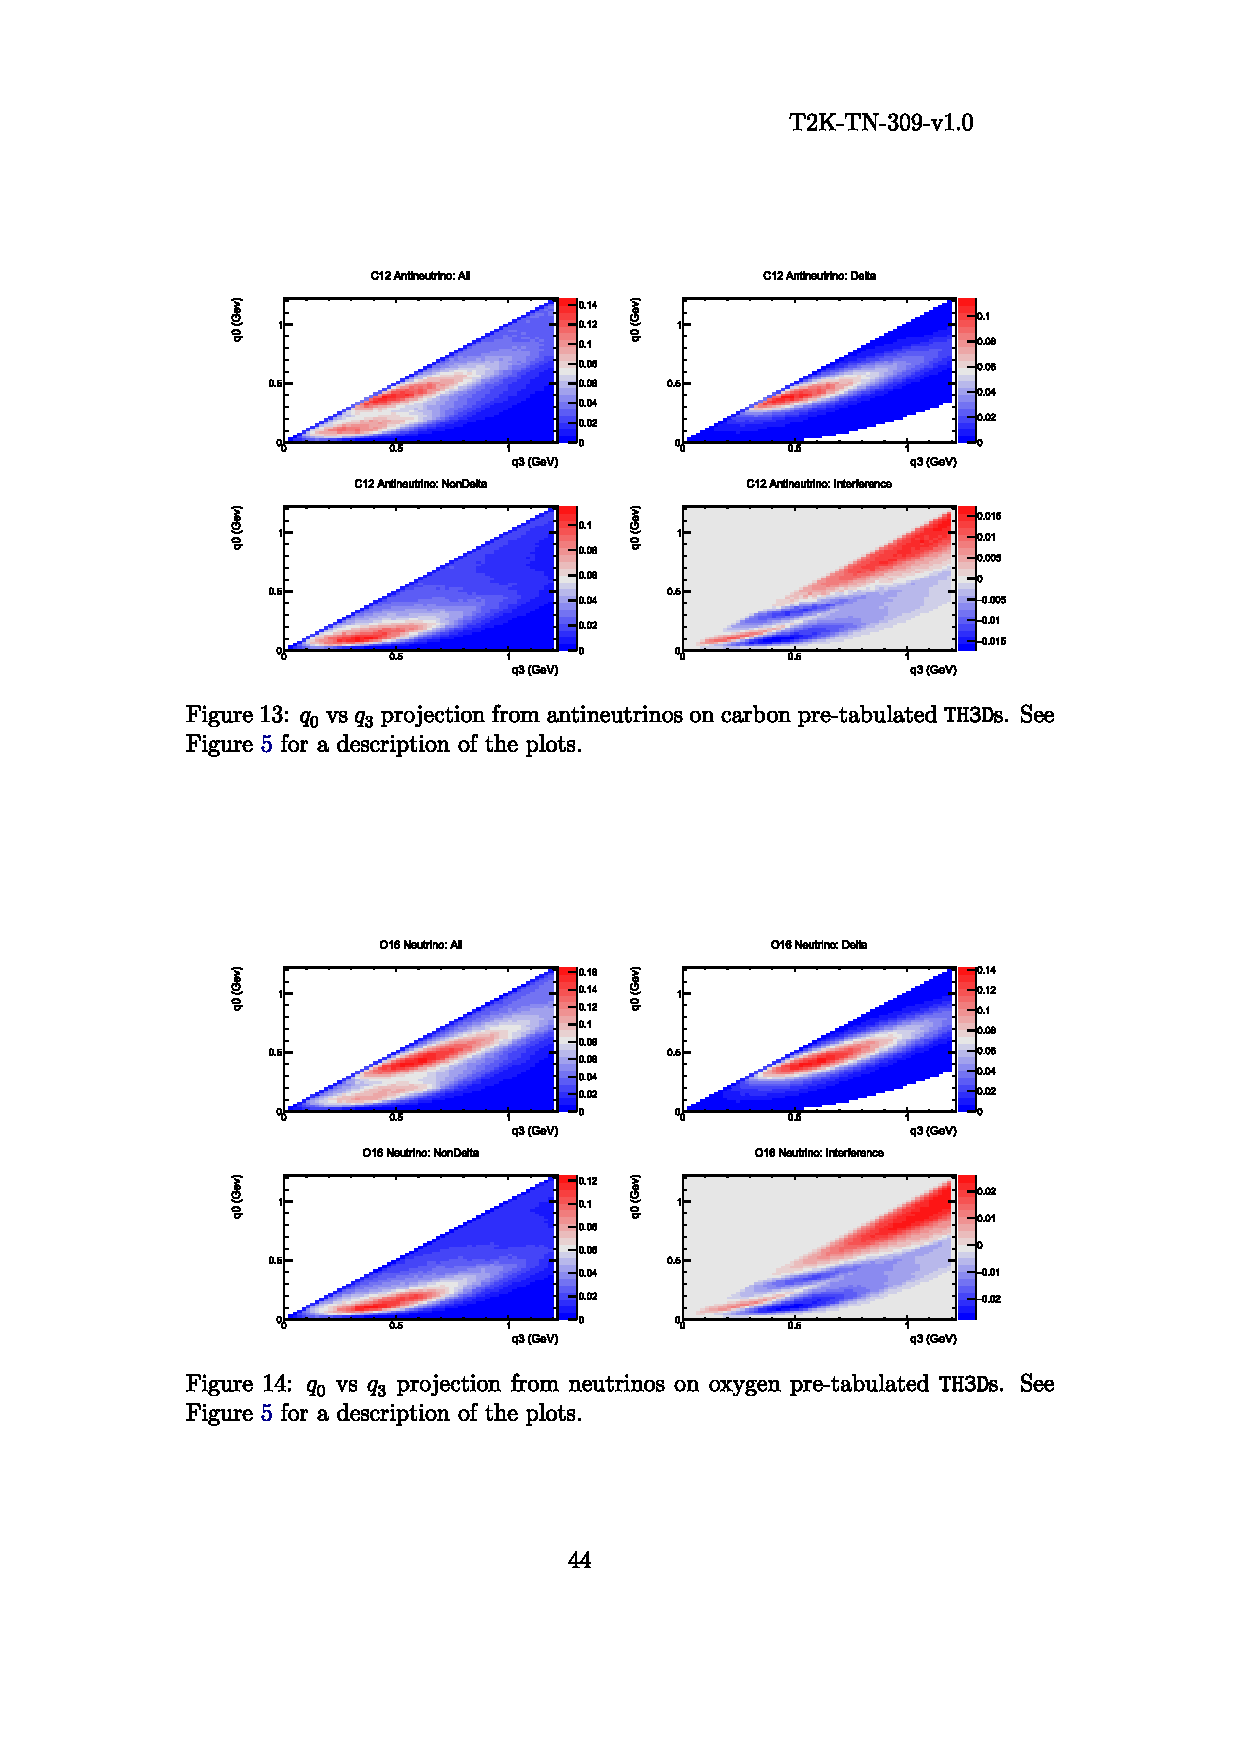
\includegraphics[page=1, trim={2cm 7cm 3cm 15.5cm}, clip, scale=1.0]{systematics/2p2h}
	\caption{Distribution of neutrino events for 2p2h and each 2p2h term in q0-q3 space \cite{NewXsecImplementation}.}
	\label{fig:2p2h_neutrino}
\end{figure}

\begin{figure}
	\includegraphics[page=2, trim={2cm 19cm 3cm 3.5cm}, clip, scale=1.0]{systematics/2p2h}
	\caption{Distribution of antineutrino events for 2p2h and each 2p2h term in q0-q3 space \cite{NewXsecImplementation}.}
	\label{fig:2p2h_antineutrino}
\end{figure}

This analysis also introduces 5 BeRPA parameters (A, B, D, E and U) to describe the collective effects of interactions between neutrinos and nucleons inside nuclei. These effects modify the $Q^2$ dependence of the neutrino-nucleus cross-section and in BeRPA are described by a cubic polynomial transitioning to an exponential above a $Q^2$ threshold, as described in \cite{NIWGUpdate2017}. Neither the 2p2h shape parameter nor the BeRPA parameters apply to interactions on free protons.

\subsection{Super-K efficiencies \& effects of intranuclear and secondary re-interactions (44 parameters)}

The Super-K detector uncertainties include the efficiencies of the fiducial volume and reduction chain, and the OD, ring-counting, PID, momentum and decay-electron cuts. These uncertainties have been evaluated by comparisons between SK-IV atmospheric data and atmospheric neutrino Monte Carlo. Ring counting errors are evaluated using $\nu_\mu$ CCQE, $\nu_\mu$ CCnQE, NC, and $\nu_e$ CC-enriched control samples from atmospheric neutrinos.  The NC PID error is evaluated using a NC-enriched control sample, obtained by not using the PID information during the selection. All the Monte Carlo control samples are fitted simultaneously to the data with a $\chi^2$ function using the selection efficiencies as fit parameters ~\cite{SuperkErrors_numu}~\cite{SuperkErrors_nue}.

Intranuclear final-state interactions (FSI) have significant effects in the T2K energy range and result in event topologies, for scattering from nuclear targets, which are drastically different from those created in neutrino scattering from free nucleons.  Uncertainties due to FSI were estimated by simultaneously varying NEUT parameters that scale interaction probabilities as described in section\ 2 of \cite{NIWGErr}. Uncertainties due to secondary pion interactions (SI) were also evaluated by allowing variations in the interaction probabilities. Details of this are given in \cite{SI}.  Since the same model is used for FSI and SI, it is possible to evaluate the uncertainties in both FSI and SI simultaneously. Details of this procedure are described in section\ 8 of \cite{NEUTnuclear}.

A list of the Super-K parameters and their errors can be found in \cref{tab:sys_sk_err}. We consider the Super-K detector efficiency and FSI+SI+PN systematics together, adding their covariance matrices linearly and evaluating the effects of these uncertainties using the Cholesky method. Details of all parameters can be found in \cite{OurRun17cCC1piJointAnalysis3Flavour}.

\begin{table}
	\begin{adjustbox}{width=\textwidth, totalheight=\textheight, keepaspectratio}
		\begin{tabular} { | c | c | c | c |  }
\hline 
Index & Parameter & Description & $1\sigma$ fractional error\\
\hline
0 & $f_{0; t, r}^{SK+FSI}$ & SKDet + FSI/SI  0; Ereco range 0.00 - 0.40 GeV; numu/numubar CCQE (1Rmu) & 0.009\\ 
1 & $f_{1; t, r}^{SK+FSI}$ & SKDet + FSI/SI  1; Ereco range 0.40 - 1.10 GeV; numu/numubar CCQE (1Rmu) & 0.007\\ 
2 & $f_{2; t, r}^{SK+FSI}$ & SKDet + FSI/SI  2; Ereco range 1.10 - 30.00 GeV; numu/numubar CCQE (1Rmu) & 0.007\\ 
3 & $f_{3; t, r}^{SK+FSI}$ & SKDet + FSI/SI  3; Ereco range 0.00 - 30.00 GeV; numu/numubar CCnQE (1Rmu) & 0.169\\ 
4 & $f_{4; t, r}^{SK+FSI}$ & SKDet + FSI/SI  4; Ereco range 0.00 - 30.00 GeV; nue/nuebar/signue CC (1Rmu) & 1.005\\ 
5 & $f_{5; t, r}^{SK+FSI}$ & SKDet + FSI/SI  5; Ereco range 0.00 - 30.00 GeV; all NC (1Rmu) & 0.658\\ 
6 & $f_{6; t, r}^{SK+FSI}$ & SKDet + FSI/SI  6; Ereco range 0.00 - 0.35 GeV; oscillated nue CC (1Re) & 0.181\\ 
7 & $f_{7; t, r}^{SK+FSI}$ & SKDet + FSI/SI  7; Ereco range 0.35 - 0.80 GeV; oscillated nue CC (1Re) & 0.036\\ 
8 & $f_{8; t, r}^{SK+FSI}$ & SKDet + FSI/SI  8; Ereco range 0.80 - 1.25 GeV; oscillated nue CC (1Re) & 0.042\\ 
9 & $f_{9; t, r}^{SK+FSI}$ & SKDet + FSI/SI  9; Ereco range 0.00 - 0.35 GeV; numu/numubar CC (1Re) & 0.300\\ 
10 & $f_{10; t, r}^{SK+FSI}$ & SKDet + FSI/SI 10; Ereco range 0.35 - 0.80 GeV; numu/numubar CC (1Re) & 0.321\\ 
11 & $f_{11; t, r}^{SK+FSI}$ & SKDet + FSI/SI 11; Ereco range 0.80 - 1.25 GeV; numu/numubar CC (1Re) & 0.393\\ 
12 & $f_{12; t, r}^{SK+FSI}$ & SKDet + FSI/SI 12; Ereco range 0.00 - 0.35 GeV; nue/nuebar CC (1Re) & 0.135\\ 
13 & $f_{13; t, r}^{SK+FSI}$ & SKDet + FSI/SI 13; Ereco range 0.35 - 0.80 GeV; nue/nuebar CC (1Re) & 0.070\\ 
14 & $f_{14; t, r}^{SK+FSI}$ & SKDet + FSI/SI 14; Ereco range 0.80 - 1.25 GeV; nue/nuebar CC (1Re) & 0.077\\ 
15 & $f_{15; t, r}^{SK+FSI}$ & SKDet + FSI/SI 15; Ereco range 0.00 - 0.35 GeV; all NC (1Re) & 0.194\\ 
16 & $f_{16; t, r}^{SK+FSI}$ & SKDet + FSI/SI 16; Ereco range 0.35 - 0.80 GeV; all NC (1Re) & 0.181\\ 
17 & $f_{17; t, r}^{SK+FSI}$ & SKDet + FSI/SI 17; Ereco range 0.80 - 1.25 GeV; all NC (1Re) & 0.472\\ 
18 & $f_{0; t, r}^{SK+FSI}RHC$ & SKDet + FSI/SI  0; Ereco range 0.00 - 0.40 GeV; numu/numubar CCQE (1Rmu); RHC & 0.009\\ 
19 & $f_{1; t, r}^{SK+FSI}RHC$ & SKDet + FSI/SI  1; Ereco range 0.40 - 1.10 GeV; numu/numubar CCQE (1Rmu); RHC & 0.007\\ 
20 & $f_{2; t, r}^{SK+FSI}RHC$ & SKDet + FSI/SI  2; Ereco range 1.10 - 30.00 GeV; numu/numubar CCQE (1Rmu); RHC & 0.007\\ 
21 & $f_{3; t, r}^{SK+FSI}RHC$ & SKDet + FSI/SI  3; Ereco range 0.00 - 30.00 GeV; numu/numubar CCnQE (1Rmu); RHC & 0.130\\ 
22 & $f_{4; t, r}^{SK+FSI}RHC$ & SKDet + FSI/SI  4; Ereco range 0.00 - 30.00 GeV; nue/nuebar/signue CC (1Rmu); RHC & 1.005\\ 
23 & $f_{5; t, r}^{SK+FSI}RHC$ & SKDet + FSI/SI  5; Ereco range 0.00 - 30.00 GeV; all NC (1Rmu); RHC & 0.657\\ 
24 & $f_{6; t, r}^{SK+FSI}RHC$ & SKDet + FSI/SI  6; Ereco range 0.00 - 0.35 GeV; oscillated nue CC (1Re); RHC & 0.108\\ 
25 & $f_{7; t, r}^{SK+FSI}RHC$ & SKDet + FSI/SI  7; Ereco range 0.35 - 0.80 GeV; oscillated nue CC (1Re); RHC & 0.036\\ 
26 & $f_{8; t, r}^{SK+FSI}RHC$ & SKDet + FSI/SI  8; Ereco range 0.80 - 1.25 GeV; oscillated nue CC (1Re); RHC & 0.057\\ 
27 & $f_{9; t, r}^{SK+FSI}RHC$ & SKDet + FSI/SI  9; Ereco range 0.00 - 0.35 GeV; numu/numubar CC (1Re); RHC & 0.349\\ 
28 & $f_{10; t, r}^{SK+FSI}RHC$ & SKDet + FSI/SI 10; Ereco range 0.35 - 0.80 GeV; numu/numubar CC (1Re); RHC & 0.342\\ 
29 & $f_{11; t, r}^{SK+FSI}RHC$ & SKDet + FSI/SI 11; Ereco range 0.80 - 1.25 GeV; numu/numubar CC (1Re); RHC & 0.417\\ 
30 & $f_{12; t, r}^{SK+FSI}RHC$ & SKDet + FSI/SI 12; Ereco range 0.00 - 0.35 GeV; nue/nuebar CC (1Re); RHC & 0.085\\ 
31 & $f_{13; t, r}^{SK+FSI}RHC$ & SKDet + FSI/SI 13; Ereco range 0.35 - 0.80 GeV; nue/nuebar CC (1Re); RHC & 0.056\\ 
32 & $f_{14; t, r}^{SK+FSI}RHC$ & SKDet + FSI/SI 14; Ereco range 0.80 - 1.25 GeV; nue/nuebar CC (1Re); RHC & 0.078\\ 
33 & $f_{15; t, r}^{SK+FSI}RHC$ & SKDet + FSI/SI 15; Ereco range 0.00 - 0.35 GeV; all NC (1Re); RHC & 0.214\\ 
34 & $f_{16; t, r}^{SK+FSI}RHC$ & SKDet + FSI/SI 16; Ereco range 0.35 - 0.80 GeV; all NC (1Re); RHC & 0.191\\ 
35 & $f_{17; t, r}^{SK+FSI}RHC$ & SKDet + FSI/SI 17; Ereco range 0.80 - 1.25 GeV; all NC (1Re); RHC & 0.465\\ 
36 & $f_{0; t, r}^{SK+FSI}MultiRing$ & SKDet + FSI/SI  0; Ereco range 0.30 - 0.80 GeV; oscillated nue CC (MultiRe); MultiRing & 0.249\\ 
37 & $f_{1; t, r}^{SK+FSI}MultiRing$ & SKDet + FSI/SI  1; Ereco range 0.80 - 1.25 GeV; oscillated nue CC (MultiRe); MultiRing & 0.215\\ 
38 & $f_{2; t, r}^{SK+FSI}MultiRing$ & SKDet + FSI/SI  2; Ereco range 0.30 - 0.80 GeV; numu/numubar CC (MultiRe); MultiRing & 0.507\\ 
39 & $f_{3; t, r}^{SK+FSI}MultiRing$ & SKDet + FSI/SI  3; Ereco range 0.80 - 1.25 GeV; numu/numubar CC (MultiRe); MultiRing & 0.236\\ 
40 & $f_{4; t, r}^{SK+FSI}MultiRing$ & SKDet + FSI/SI  4; Ereco range 0.30 - 0.80 GeV; nue/nuebar CC (MultiRe); MultiRing & 0.244\\ 
41 & $f_{5; t, r}^{SK+FSI}MultiRing$ & SKDet + FSI/SI  5; Ereco range 0.80 - 1.25 GeV; nue/nuebar CC (MultiRe); MultiRing & 0.235\\ 
42 & $f_{6; t, r}^{SK+FSI}MultiRing$ & SKDet + FSI/SI  6; Ereco range 0.30 - 0.80 GeV; all NC (MultiRe); MultiRing & 0.983\\ 
43 & $f_{7; t, r}^{SK+FSI}MultiRing$ & SKDet + FSI/SI  7; Ereco range 0.80 - 1.25 GeV; all NC (MultiRe); MultiRing & 0.524\\ 
44 & $f_{E; r}^{SK}$ & SK energy scale & 0.024\\ 

\hline

\end{tabular}
	\end{adjustbox}
	\caption{Summary of SK detector + FSI + SI + PN systematics included in the VALOR joint fit analysis.}
	\label{tab:sys_sk_err}
\end{table}

\subsection{Super-K energy scale (1 parameter)}

The systematic parameter $f_{E; r}^{SK}$ is included to estimate the effects of uncertainty in the Super-K reconstructed energy scale.  This uncertainty is estimated to be 2.4\% \cite{SuperkEScale2013}; its effects are calculated by scaling the bin edges of the MC templates and, assuming uniform distribution of events within the bins, calculating the number of events gained from/lost to other bins (including bins that are not immediately adjacent). This systematic is applied after all other systematics have been applied, because it affects reconstructed rather than true energy, does not commute with spline-based systematics, which are generated without consideration of energy scale variation and also does not commute with the other Super-K systematics, which are determined from data without any energy scale variation.

\subsection{Oscillation parameters and mass hierarchy (7 parameters)}

The 3-flavour oscillation probability is used.  All the nuisance oscillation parameters, i.e. those parameters which are not shown in a given contour, are marginalised except the mass hierarchy which is fixed to either normal or inverted hierarchy.

For $\sin^2 \theta_{13}$ two different priors can be used, depending on whether the reactor constraint is applied, denoted as ``reactors", when applied and ``T2K only" when not applied.

\begin{table}
	\centering
	\begin{tabular}{| c | c | c | c |}
 	\hline
Parameter(s)	& Prior		& Range    \\
\hline
$\sin^{2}\theta_{23}$	&  uniform 	& $[0.3; 0.7]$      \\
$\sin^{2} 2 \theta_{13}$ ($\sin^{2} \theta_{13}$) reactors		&  gaussian 		& $0.0857 \pm 0.0046$ 	\\
$\sin^{2} 2 \theta_{13}$ ($\sin^{2} \theta_{13}$) T2K only	   	&  uniform		& $[0; 0.4]$ 	\\
$\sin^{2} 2 \theta_{12}$  								&  gaussian 		& $0.846 \pm 0.021$ \\
$|\Delta m^{2}_{32}|$ (NH) / $|\Delta m^{2}_{13}|$ (IH)      		&  uniform		& $ [2.3; 2.7] \times 10^{-3}~\mbox{eV}^2/\mbox{c}^4$		 \\
$\Delta m^{2}_{21}$      								&  gaussian 		& $(7.53 \pm 0.18) \times 10^{-5}~\mbox{eV}^2/\mbox{c}^4$		\\
$\delta_{CP}$                                               				&  uniform 	& $[-\pi; +\pi]$ \\
Mass Hierarchy										&  fixed 		& NH or IH \\  
\hline
\end{tabular}
\caption{
Treatment of the oscillation parameters in the $\nu/\bar{\nu}$ joint analysis. All the gaussian priors are from \cite{pdg_2014}. The parameter $\sin^{2} 2 \theta_{13}$ can be constrained with the measurement of reactor experiments using the gaussian prior, otherwise a uniform prior is used and the measurement relies only on the T2K data. The nominal values of $\sin^2 2 \theta_{13}$, $\sin^2 2 \theta_{12}$ and $\Delta m^2_{21}$ are from \cite{pdg_2014}, while all the other oscillation parameter values corresponds to the most probable values obtained by the Bayesian analysis on the T2K run 1-4 neutrino mode data \cite{T2KLongPaper}. The mass hierarchy is not marginalised but fixed to either NH or IH.
}
\label{tab:osc_param_priors}
\end{table}

\subsection{Systematic error on Super-K predictions}
\label{sec:systematics:errortables}

The effect of each category of systematic parameter on the expected event rate for Super-K sample is given in \crefrange{tab:sk_errors_1Rmu}{tab:sk_errors_MultiRe} (details of per-sample event rates for $1\sigma$ and $3\sigma$ variations of each independent systematic parameter can be found in \cref{app:sysvar}). The mean and RMS of 10000 throws of the respective systematics (with correlations taken into account) is computed for each sample and in the case of pre-BANFF and post-BANFF errors. When not measuring the effect of oscillation parameters variations, the oscillation parameters are fixed at Asimov A values (see \cref{sec:asimov_definition}).

For the measurement of $\delta_{CP}$ it is important to understand the effect of the systematic uncertainties on the ratio of the number of events between neutrino and antineutrino mode samples. If correlations do not reproduce the physics correctly, a fake asymmetry between neutrino and antineutrino oscillations can be seen. Furthermore, if correlations exist but are not taken into account, the measurement of $\delta_{CP}$ could be biased. The true value of $\delta_{CP}$ determines whether correlations or anti-correlations between systematic parameters have the greatest effect in hiding any oscillation asymmetry. In particular, if true $\delta_{CP} = \pm \pi/2$ then anti-correlation in the $e$-like samples could hide any oscillation asymmetry. Alternatively, in the case that true $\delta_{CP} \sim 0$ it is uncorrelated parameters that reduce the sensitivity to $\delta_{CP}$. The uncertainties on the ratios between neutrino and antineutrino mode events due to the systematic parameters are shown in \cref{tab:sk_errors_summary}. The most critical systematic parameters are $\sigma_{\nu_e}$ and $\sigma_{\bar{\nu}_e}$ which are applied respectively to $\nu_e$ and $\bar{\nu}_e$ events. Their fractional error from the BANFF covariance matrix is 2.83\% (see \cref{tab:sys_xsec_err}) and they are partially anti-correlated with non-diagonal elements in the covariance matrix of -0.0004.

It can be seen in \crefrange{tab:sk_errors_1Rmu}{tab:sk_errors_MultiRe} (\Cref{app:sk_errors}) that the reduction in the error on flux and constrained cross-section systematics achieved through the BANFF fit reduces the fractional error due to all systematics from $\sim 14\%$ to $\sim 4\%$ and $\sim 11\%$ to $\sim 3\%$ in the neutrino- and antineutrino-mode $\mu$-like samples respectively, from $\sim 16\%$ to $\sim 7\%$ and $\sim 13\%$ to $\sim 8\%$ in the neutrino- and antineutrino-mode $e$-like samples respectively, and from $\sim 25\%$ to $\sim 22\%$ in the \nueCConepi{}-like sample. A summary of the effects of the systematic errors is given in \cref{tab:sk_errors_summary}.

\begin{table}[H]
	\centering
	\begin{tabular}{|l||l|l||l|l|l|l|l|}
		\hline
		& \multicolumn{2}{c||}{\textbf{1-Ring $\mu$}} & \multicolumn{4}{c|}{\textbf{1-Ring $e$}} \\ \hline
		Error source & FHC & RHC & FHC & RHC & FHC 1 d.e. & FHC/RHC \\ \hline\hline
		SK Detector & 1.86 & 1.51 & 3.03 & 4.22 & 16.69 & 1.60 \\ \hline
		SK FSI+SI+PN & 2.20 & 1.98 & 3.01 & 2.31 & 11.43 & 1.57 \\ \hline
		Flux + Xsec constrained & 3.22 & 2.72 & 3.22 & 2.88 & 4.05 & 2.50 \\ \hline
		$\sigma(\nu_e)/\sigma(\bar{\nu}_e)$ & 0.00 & 0.00 & 2.63 & 1.46 & 2.62 & 3.03 \\ \hline
		NC1$\gamma$ & 0.00 & 0.00 & 1.08 & 2.59 & 0.33 & 1.49 \\ \hline
		NC Other & 0.25 & 0.25 & 0.14 & 0.33 & 0.98 & 0.18 \\ \hline
		Osc & 0.04 & 0.03 & 3.86 & 3.60 & 3.78 & 0.79 \\ \hline\hline
		All Systematics & 4.40 & 3.76 & 6.10 & 6.51 & 20.94 & 4.77 \\ \hline
		All with osc & 4.40 & 3.76 & 7.27 & 7.44 & 21.24 & 4.85 \\ \hline
	\end{tabular}
	\caption
	{
	Percentage error on event rate by error source and sample. Final column is the percentage error on the ratio of FHC/RHC events in the one-ring $e$ sample.
	}
	\label{tab:sk_errors_summary}
\end{table}


The error envelopes corresponding to \crefrange{tab:sk_errors_1Rmu}{tab:sk_errors_MultiRe} are shown in \crefrange{fig:sk_envelopes_all}{fig:sk_envelopes_xsec_ncoth_b}. These error envelopes are determined by performing \num{1e4} correlated throws of the systematic parameter group under consideration and plotting the mean and Gaussian $1\sigma$ error resulting.

\begin{figure*}
	\center
	\begin{subfigure}[b]{0.49\textwidth}
		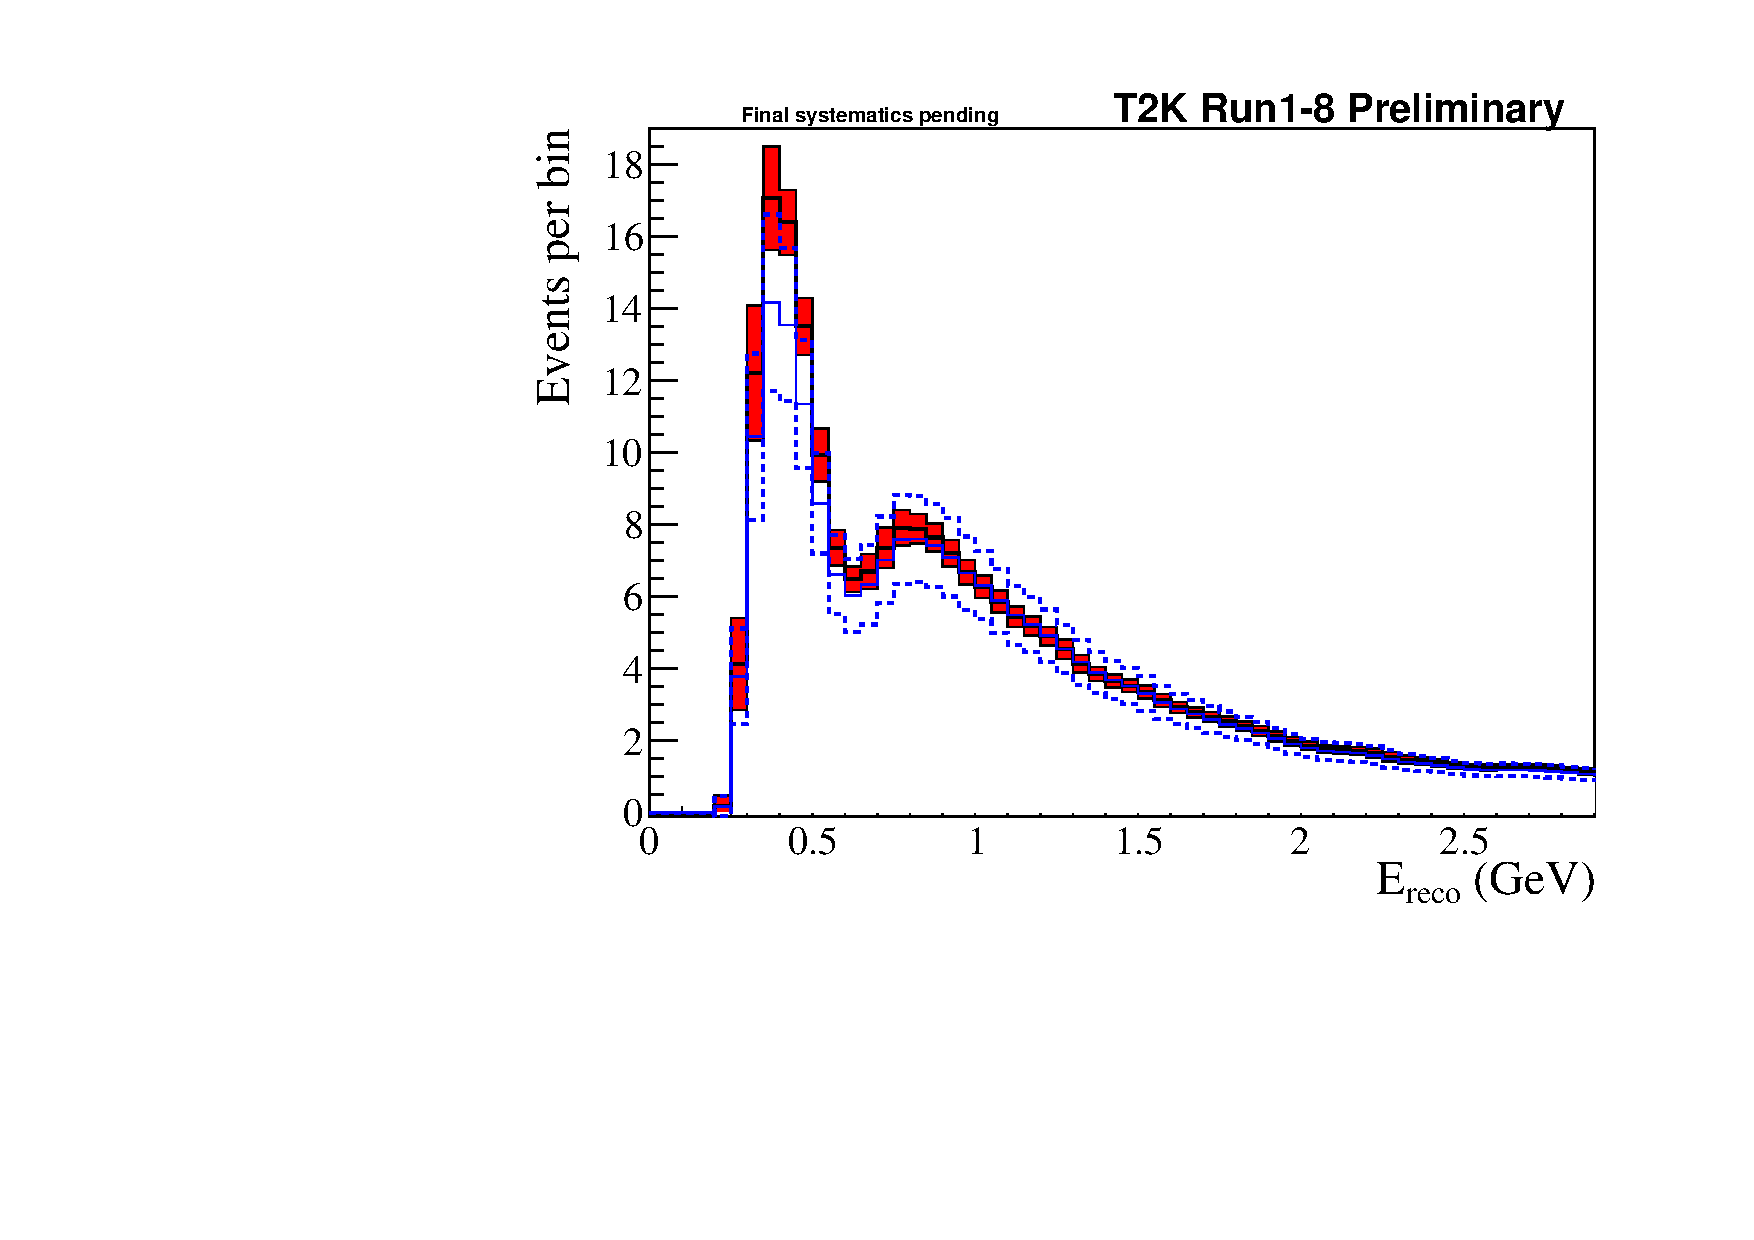
\includegraphics[width=0.9\textwidth]{systematics/envelopes/sk_errors/sk_error_table_1Rmu_all_envelope}
		\caption{Muon-like, neutrino mode}
	\end{subfigure}
	\begin{subfigure}[b]{0.49\textwidth}
		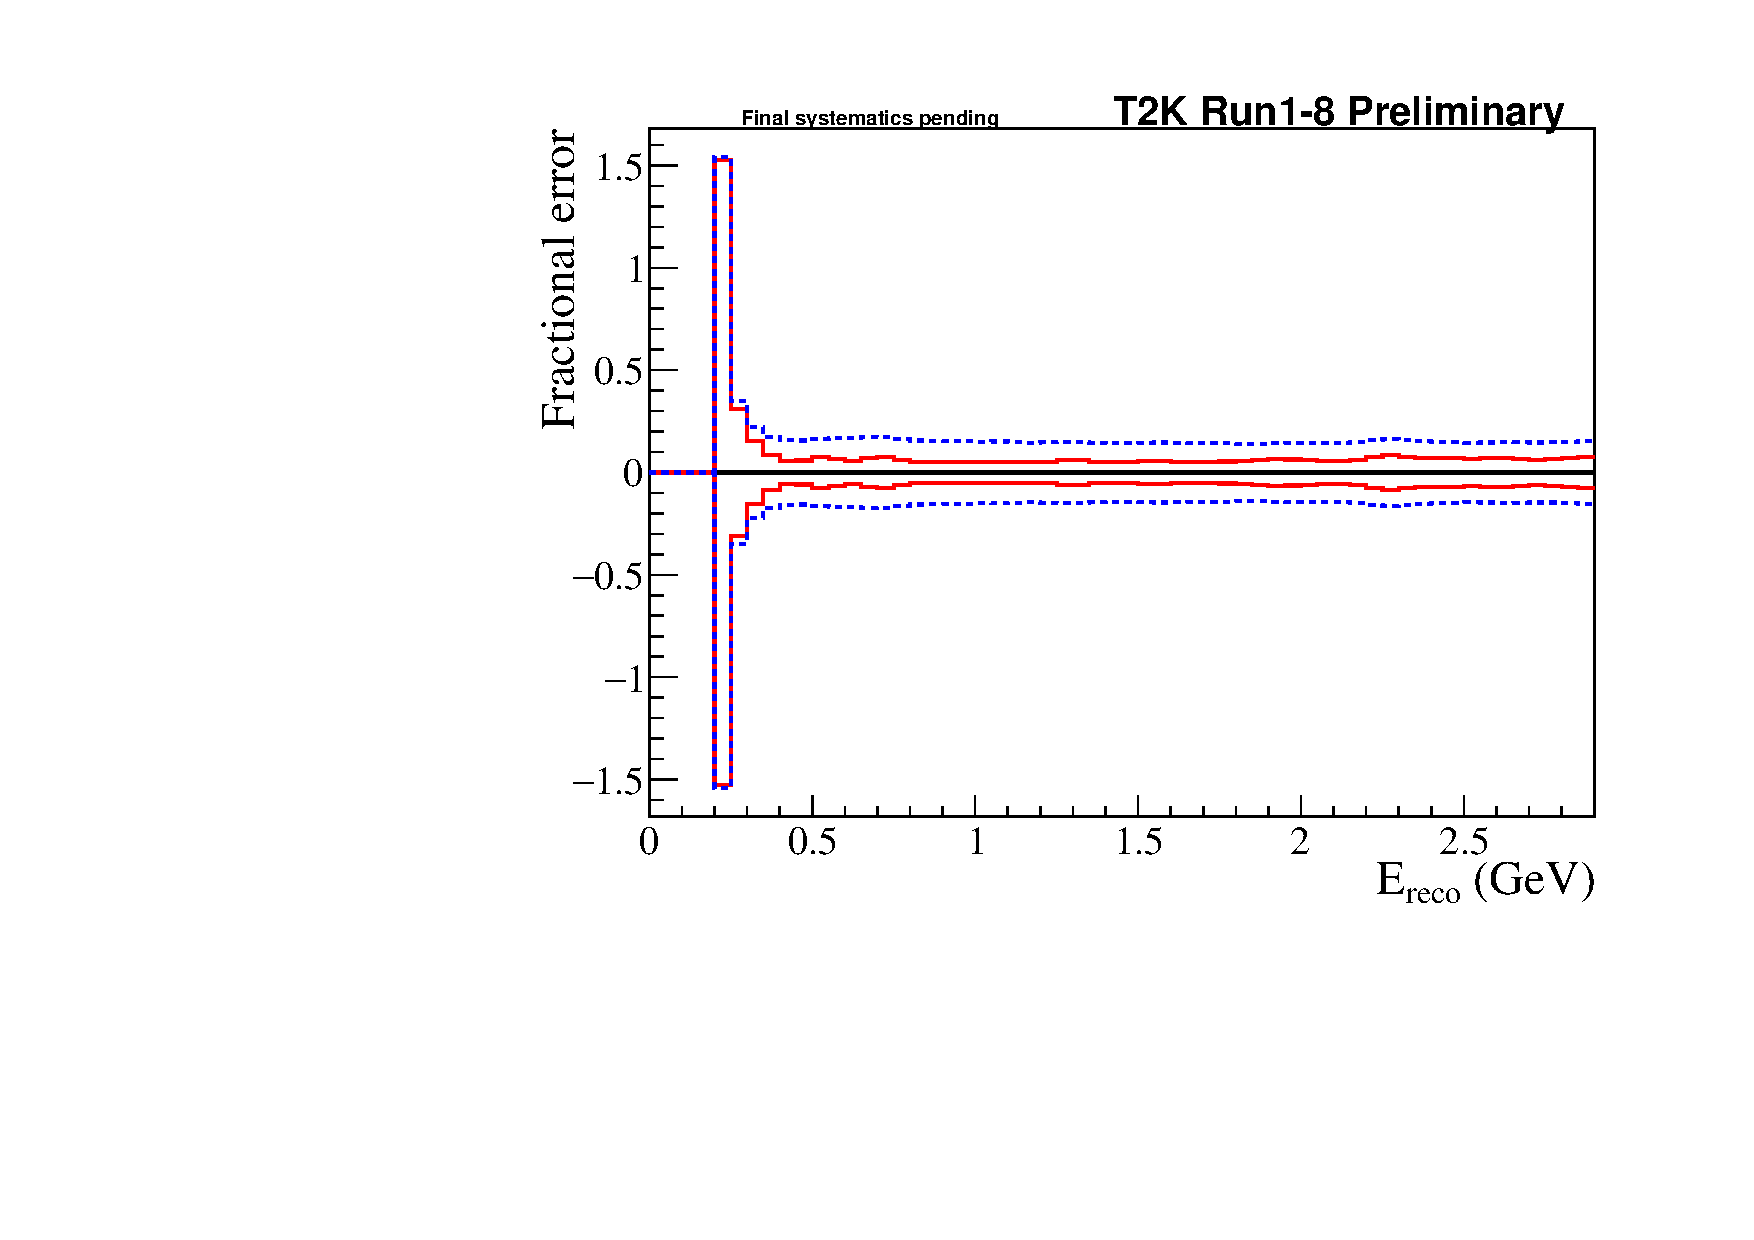
\includegraphics[width=0.9\textwidth]{systematics/envelopes/sk_errors/sk_error_table_1Rmu_all_envelope_fractional}
		\caption{Muon-like, neutrino mode}
	\end{subfigure}
	\begin{subfigure}[b]{0.49\textwidth}
		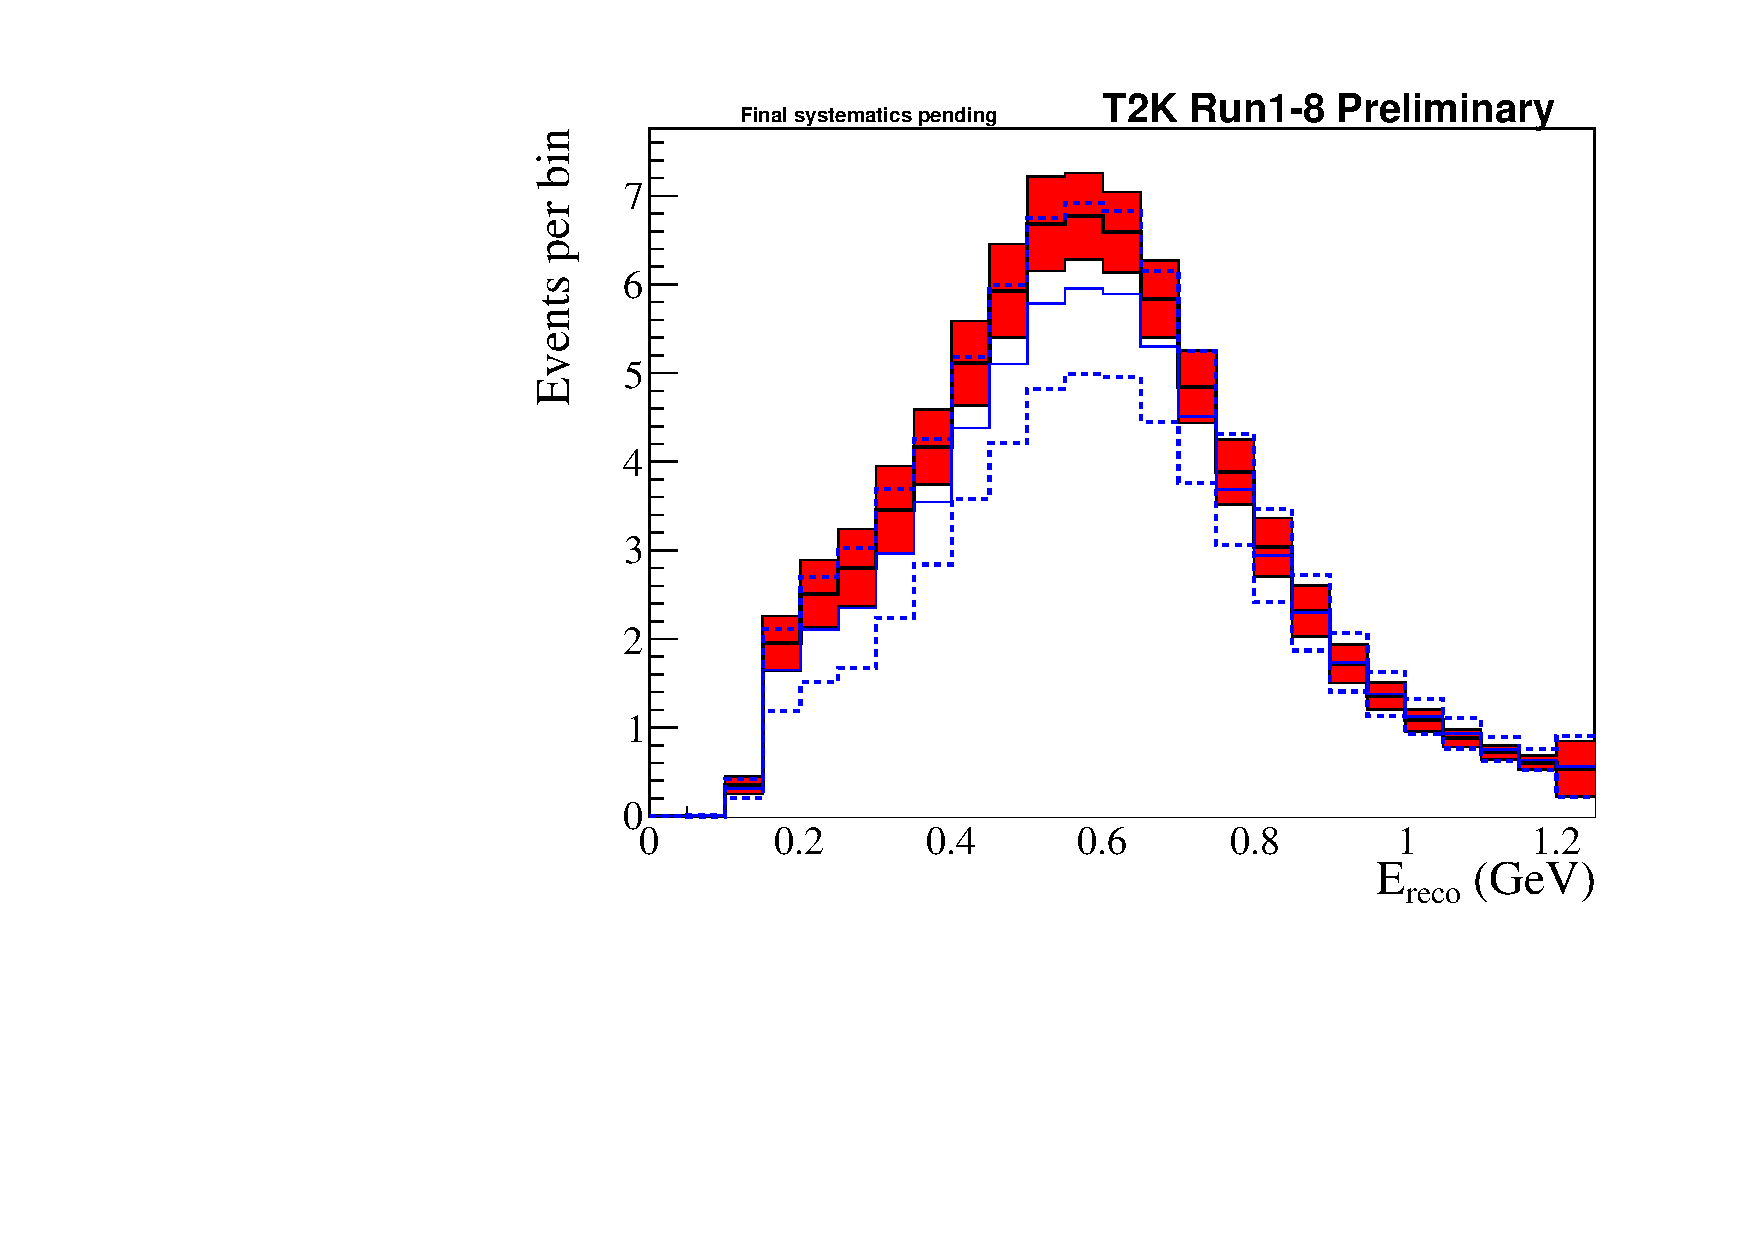
\includegraphics[width=0.9\textwidth]{systematics/envelopes/sk_errors/sk_error_table_1Re_all_envelope}
		\caption{Electron-like, neutrino mode}
	\end{subfigure}
	\begin{subfigure}[b]{0.49\textwidth}
		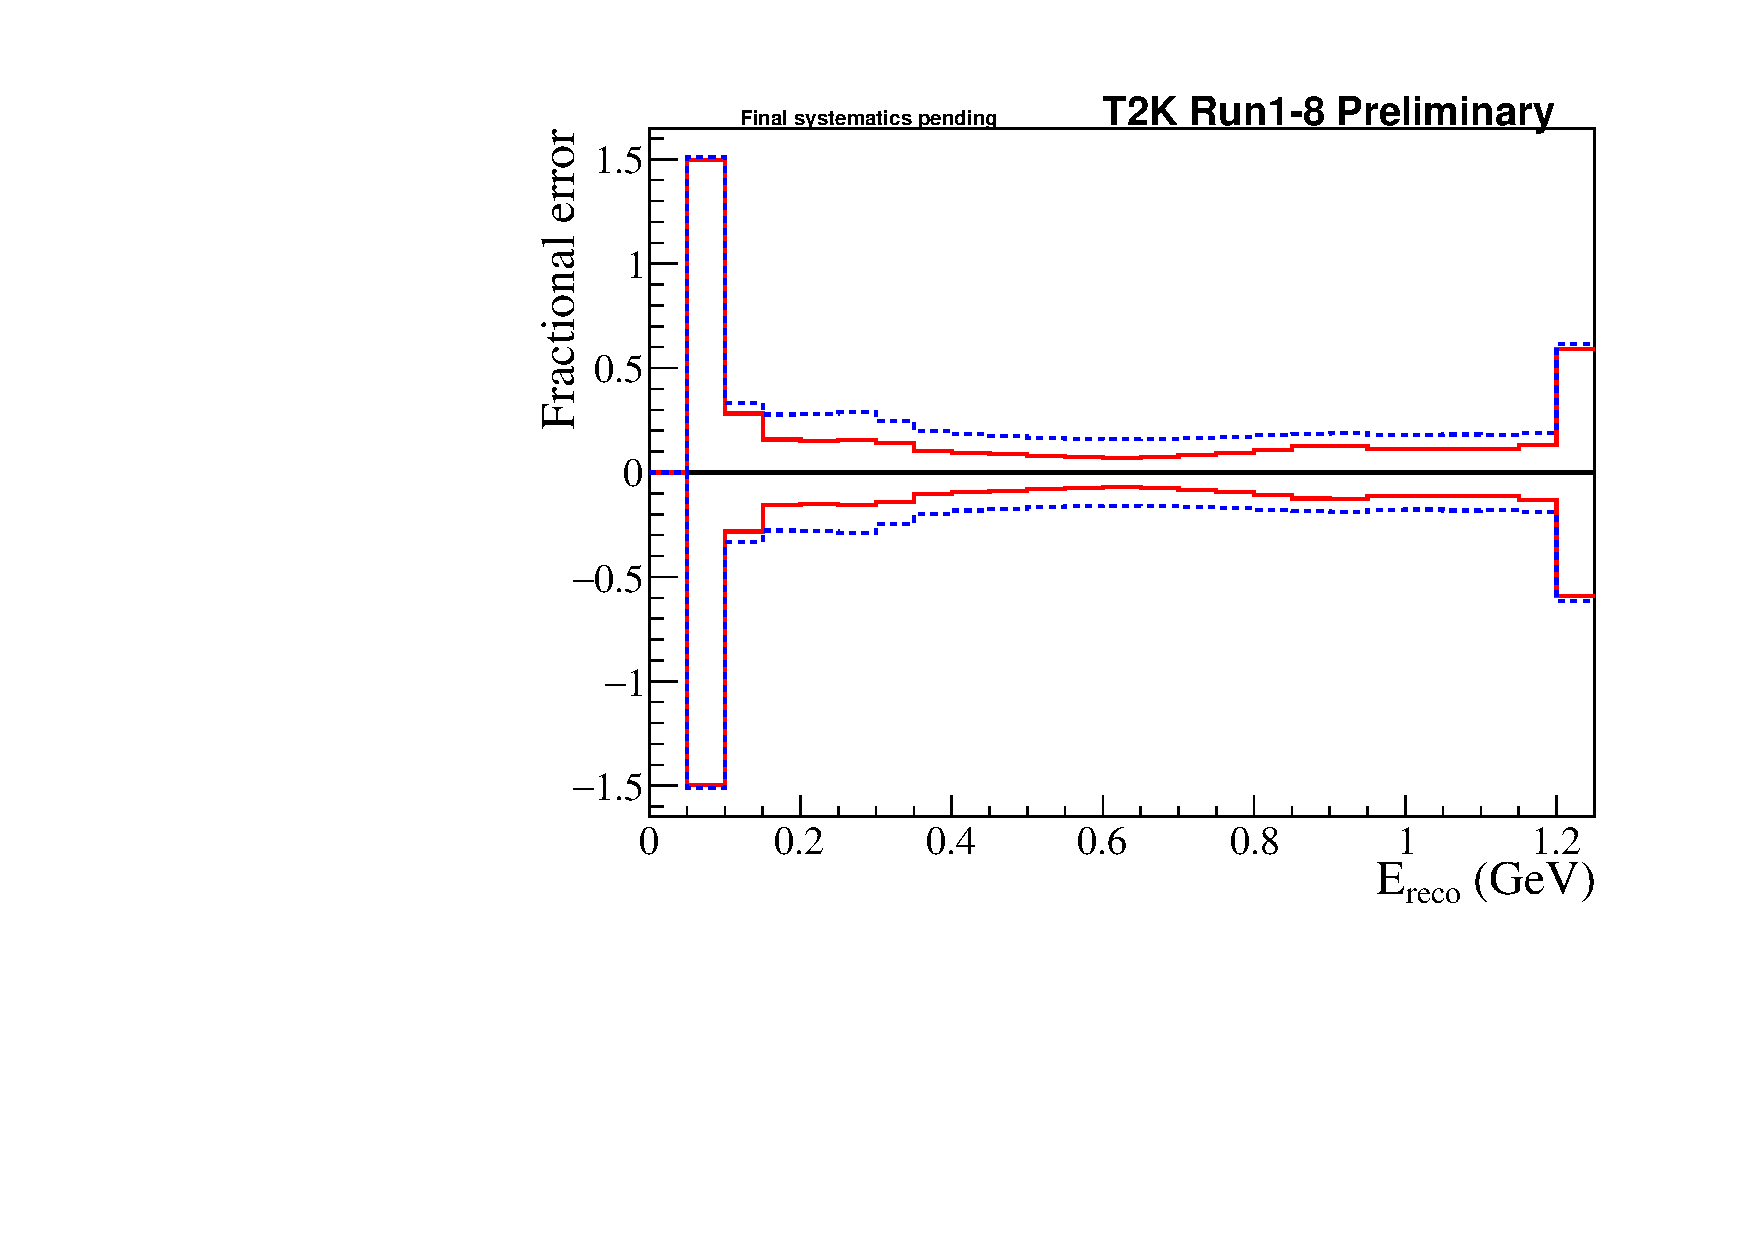
\includegraphics[width=0.9\textwidth]{systematics/envelopes/sk_errors/sk_error_table_1Re_all_envelope_fractional}
		\caption{Electron-like, neutrino mode}
	\end{subfigure}
	\begin{subfigure}[b]{0.49\textwidth}
		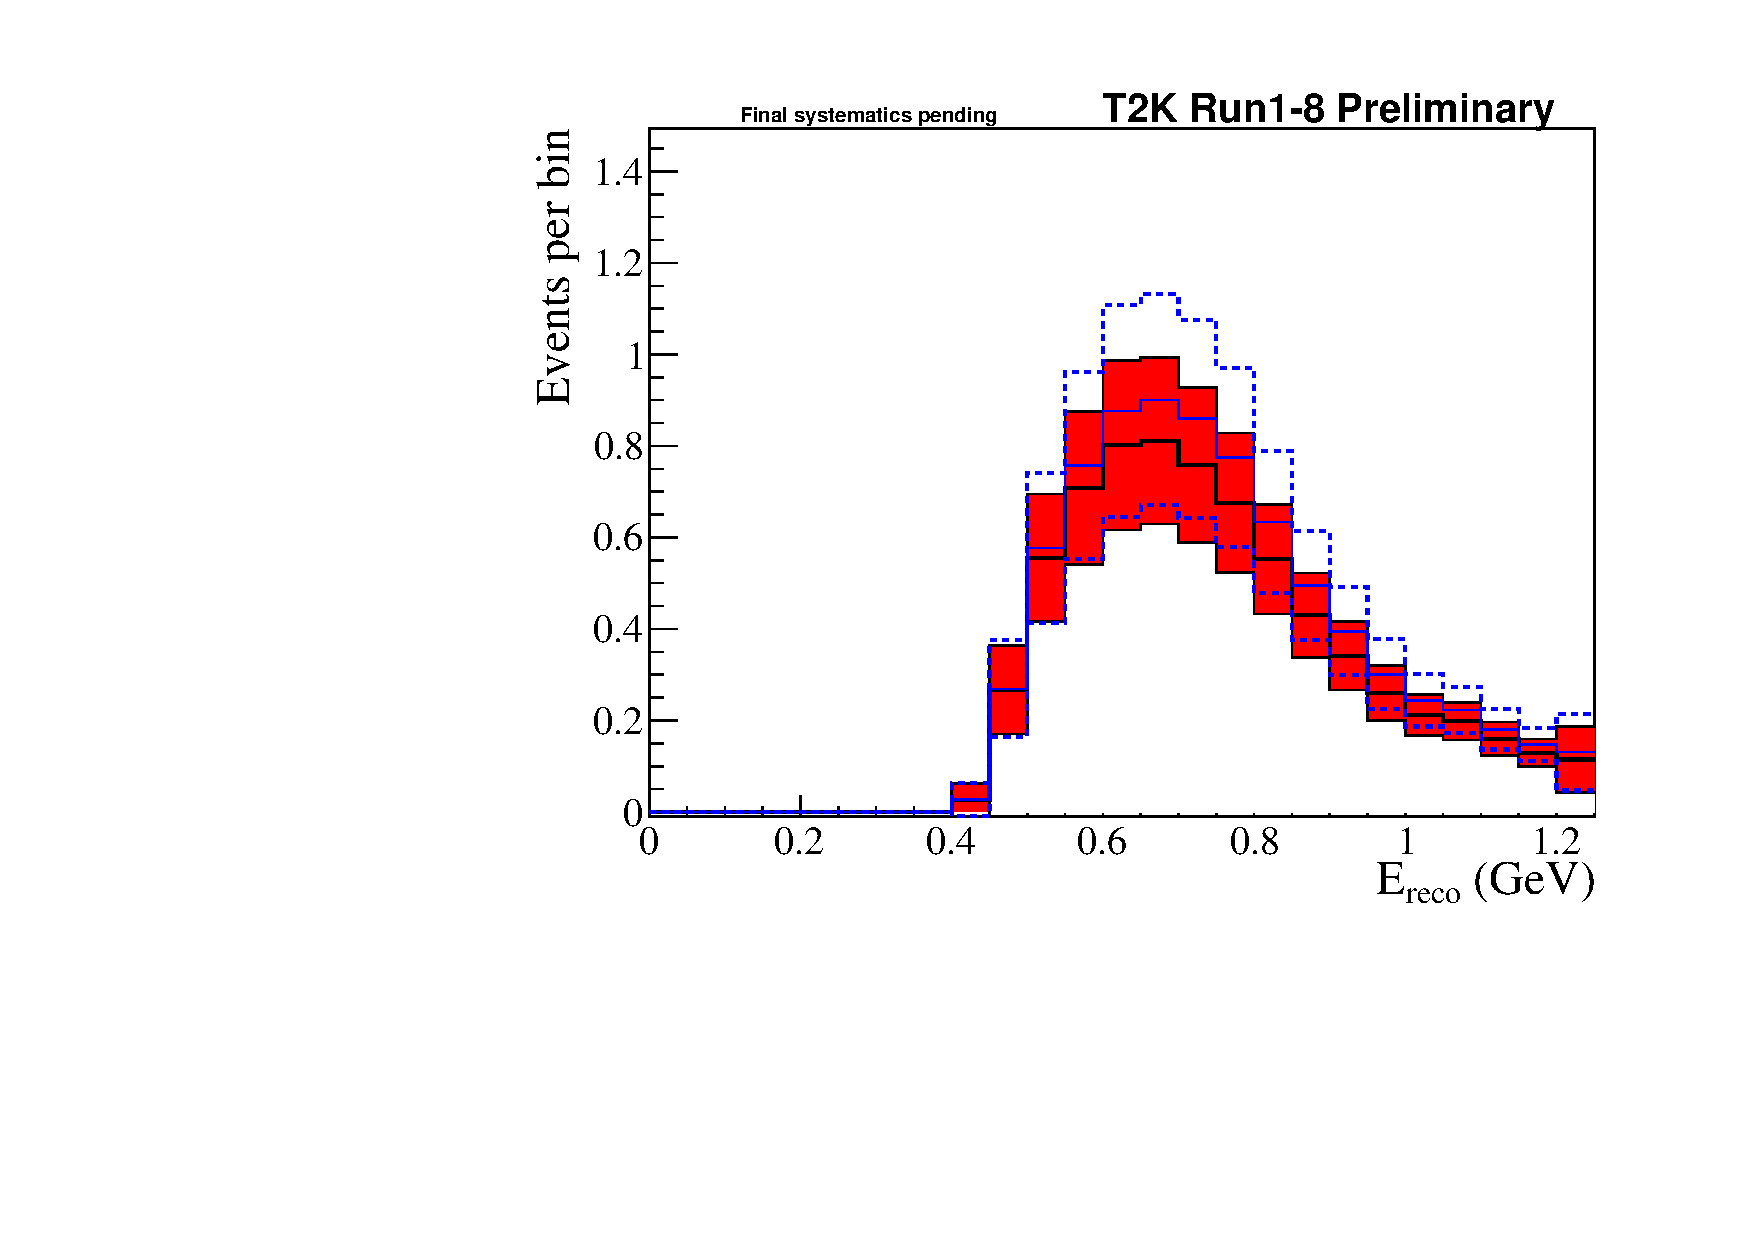
\includegraphics[width=0.9\textwidth]{systematics/envelopes/sk_errors/sk_error_table_MultiRe_all_envelope}
		\caption{\nueCConepi-like, neutrino mode}
	\end{subfigure}
	\begin{subfigure}[b]{0.49\textwidth}
		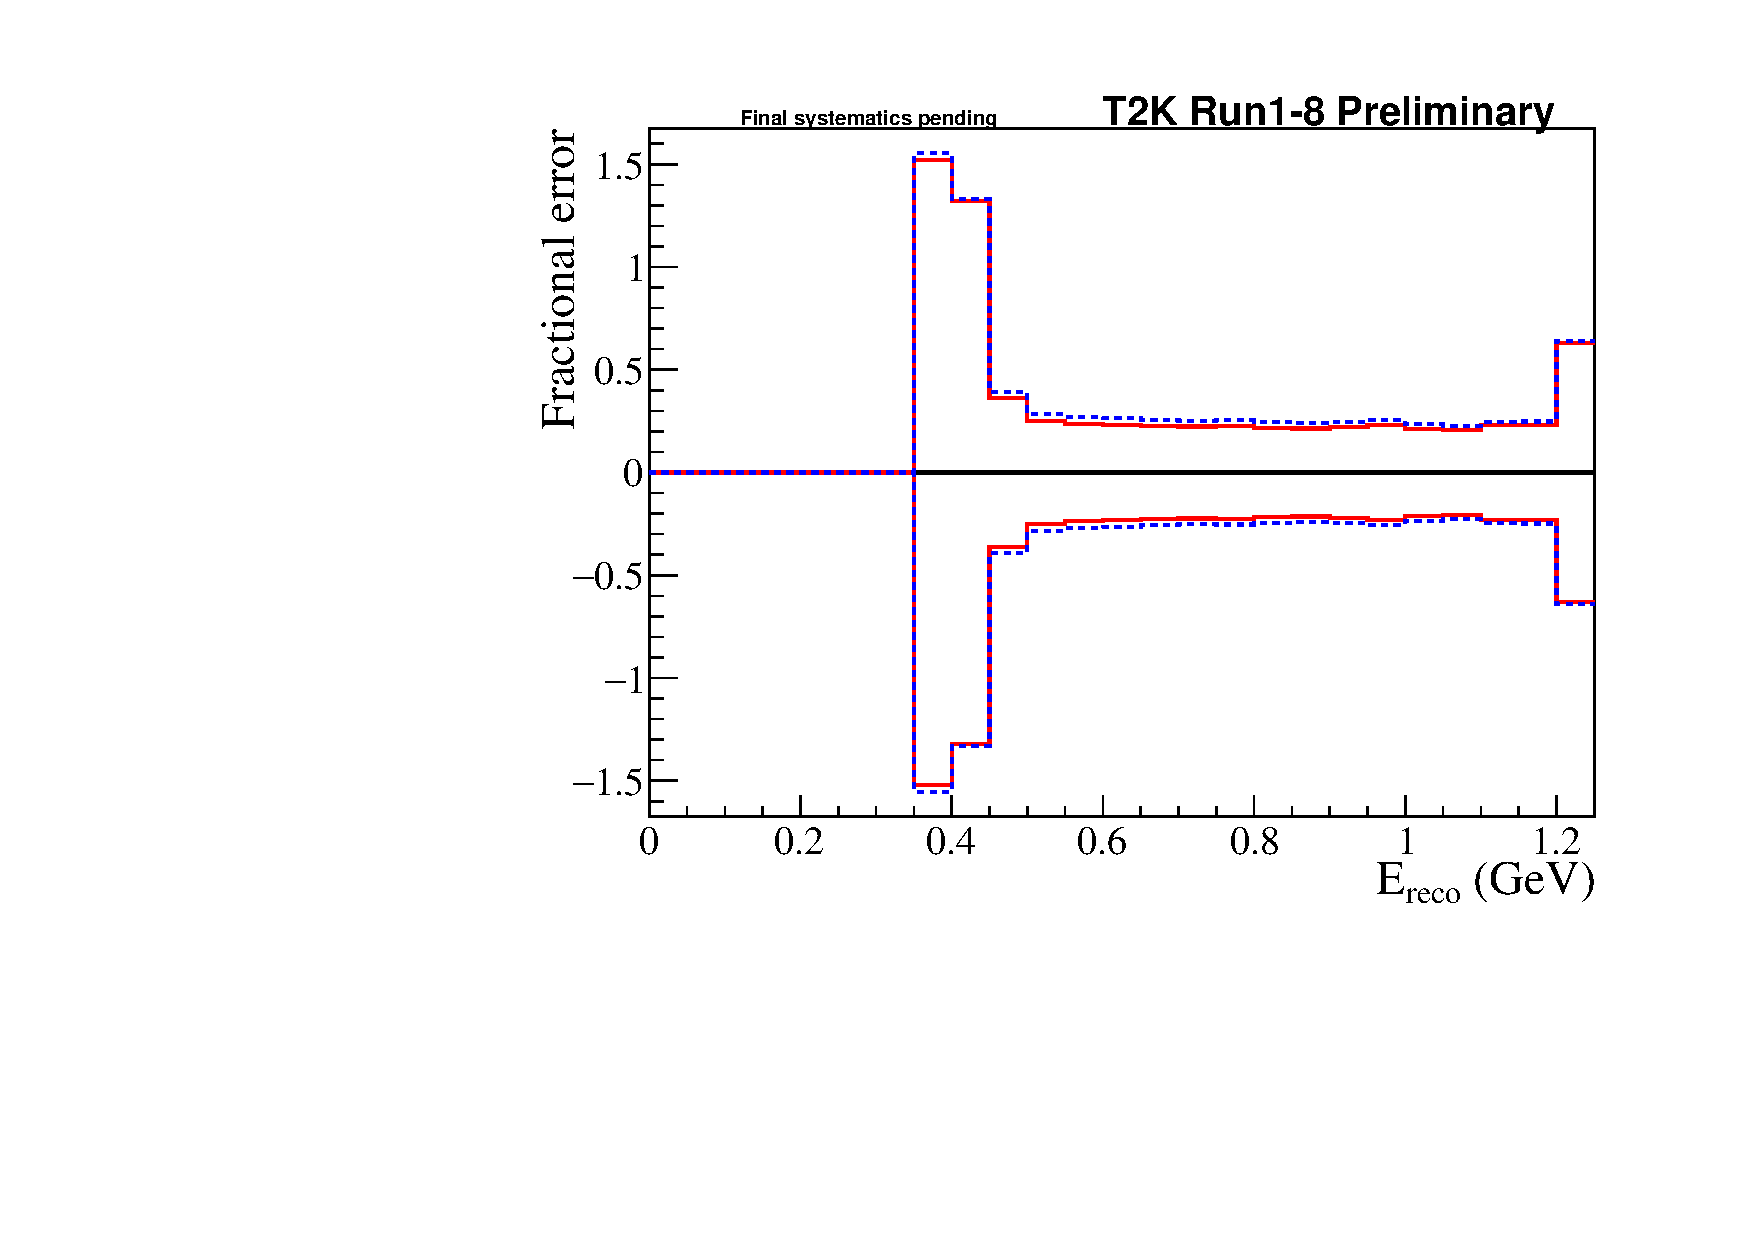
\includegraphics[width=0.9\textwidth]{systematics/envelopes/sk_errors/sk_error_table_MultiRe_all_envelope_fractional}
		\caption{\nueCConepi-like, neutrino mode}
	\end{subfigure}
	\caption {
		Error envelopes (left) and fractional errors (right) for the reconstructed neutrino energy spectrum for all systematic parameters for pre-BANFF (blue) and post-BANFF (red) errors. \num{1e4} toys are generated for the Asimov data set A with randomized systematic parameters with correlations taken into account. Since \deltacp, \ssqthtwothree, \dmsqtwothree and the mass hierarchy will be measured, only the uncertainty on \ssqthonethree, \ssqthonetwo and \dmsqonetwo are taken into account.
	}
	\label{fig:sk_envelopes_all}
\end{figure*}
\clearpage
\begin{figure*}
	\center
	\begin{subfigure}[b]{0.49\textwidth}
		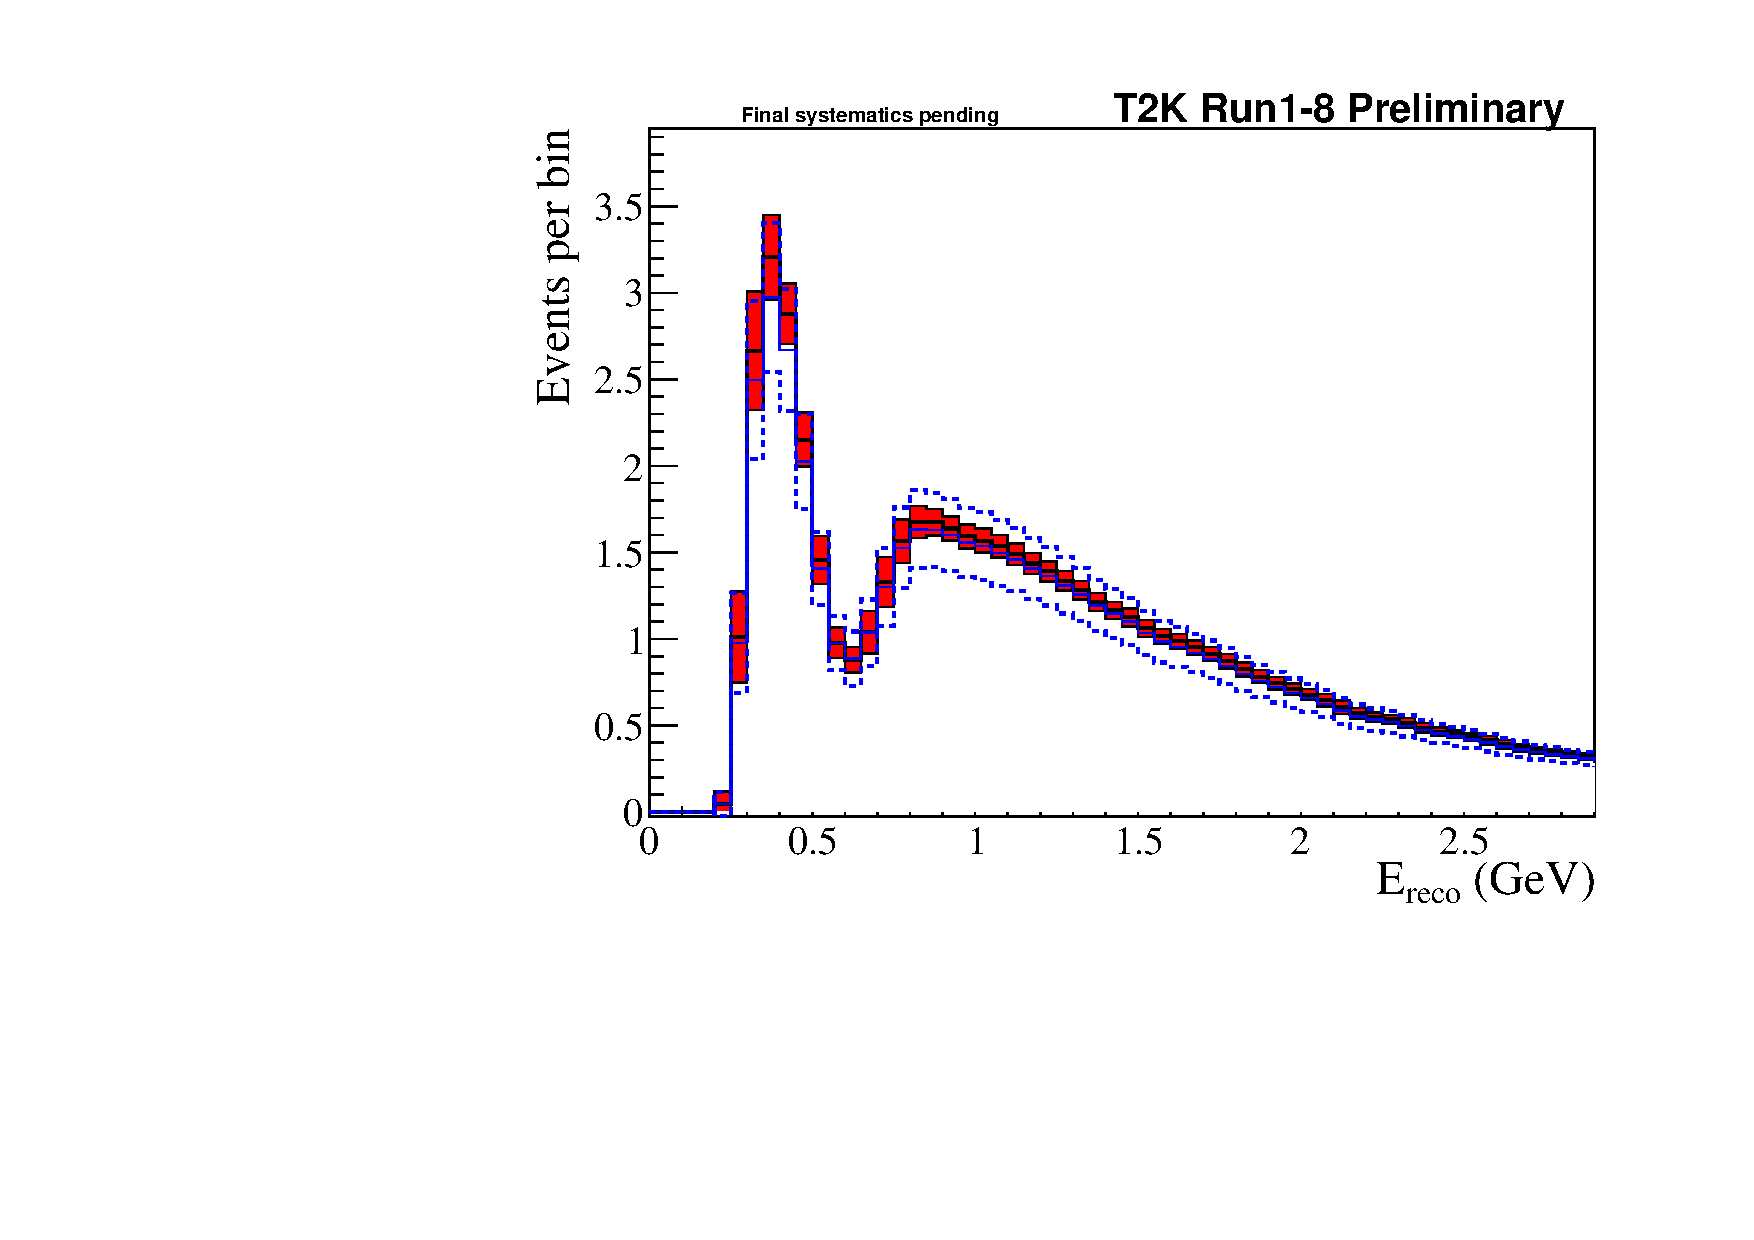
\includegraphics[width=0.9\textwidth]{systematics/envelopes/sk_errors/sk_error_table_RHC1Rmu_all_envelope}
		\caption{Muon-like, antineutrino mode}
	\end{subfigure}
	\begin{subfigure}[b]{0.49\textwidth}
		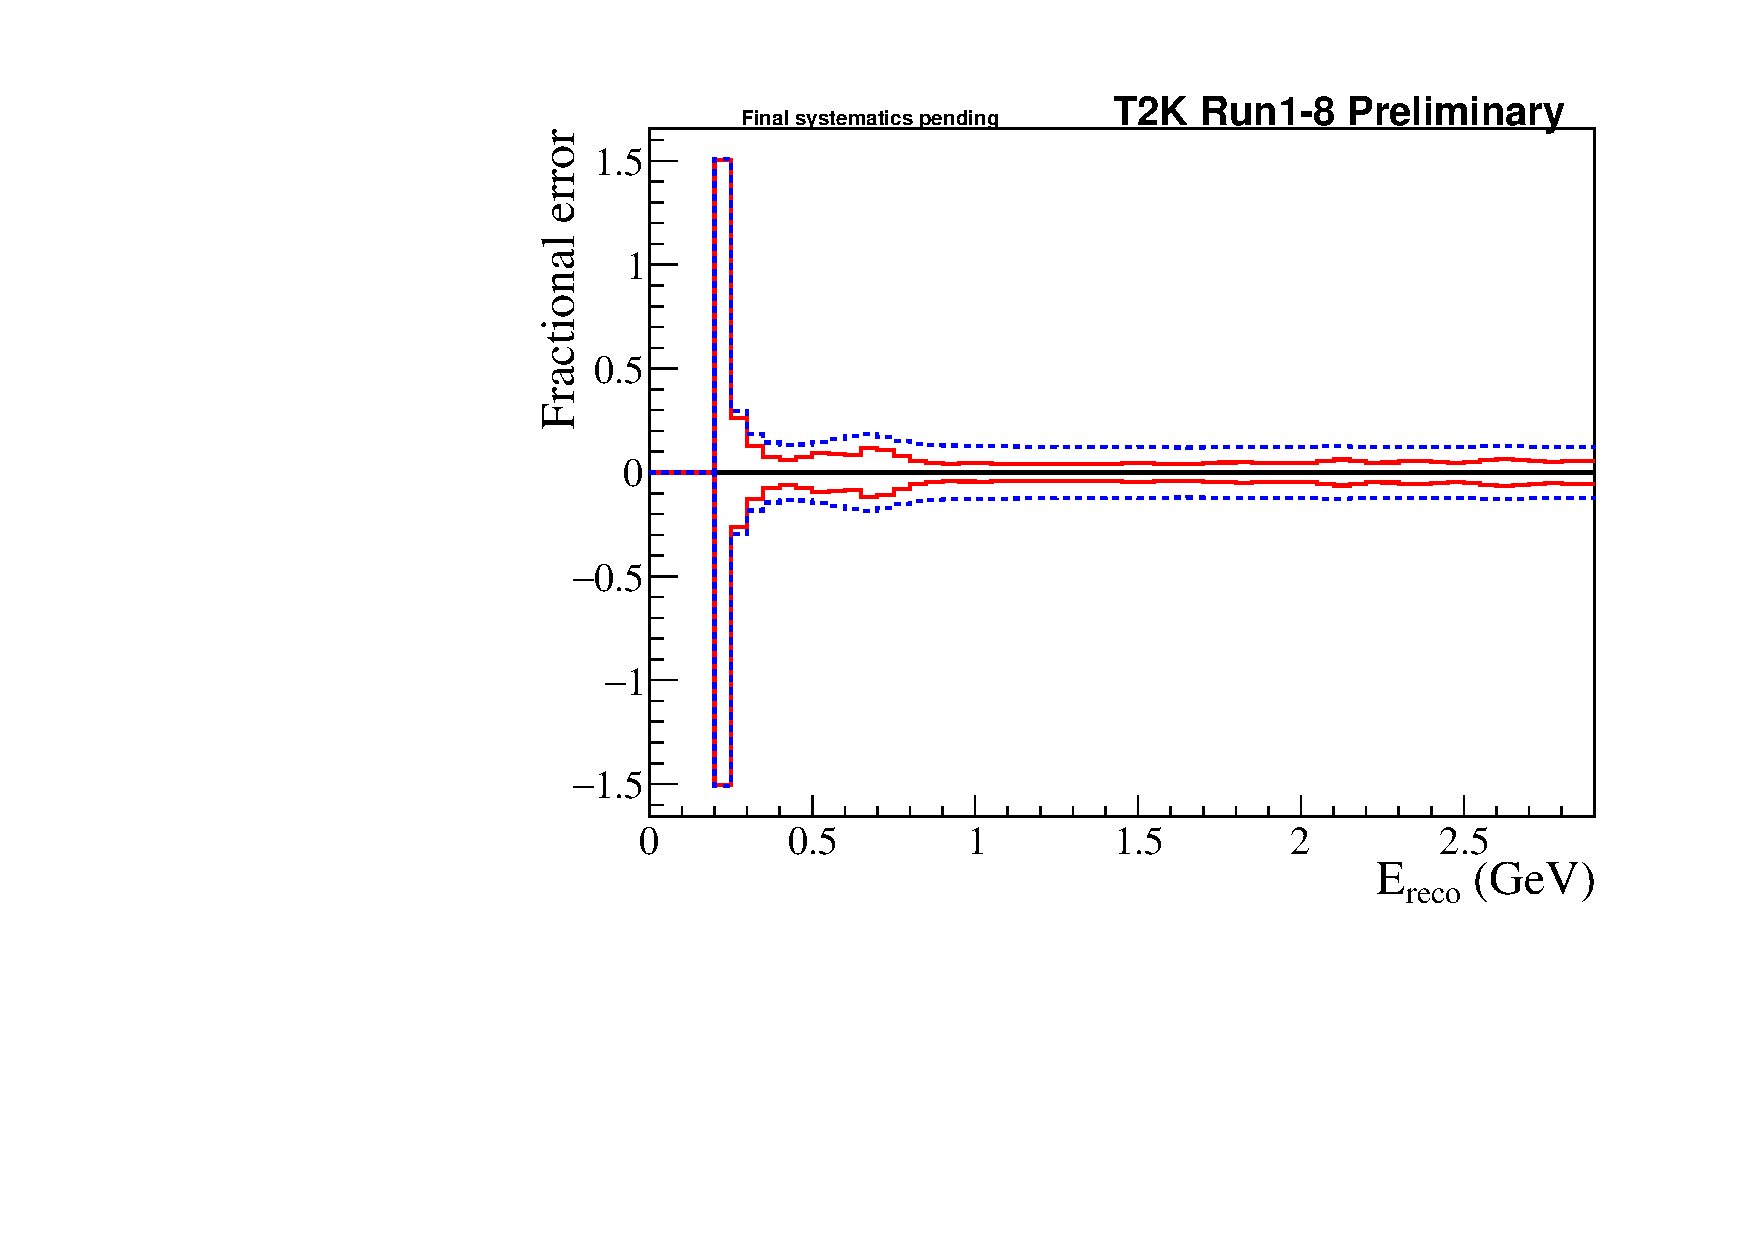
\includegraphics[width=0.9\textwidth]{systematics/envelopes/sk_errors/sk_error_table_RHC1Rmu_all_envelope_fractional}
		\caption{Muon-like, antineutrino mode}
	\end{subfigure}
	\begin{subfigure}[b]{0.49\textwidth}
		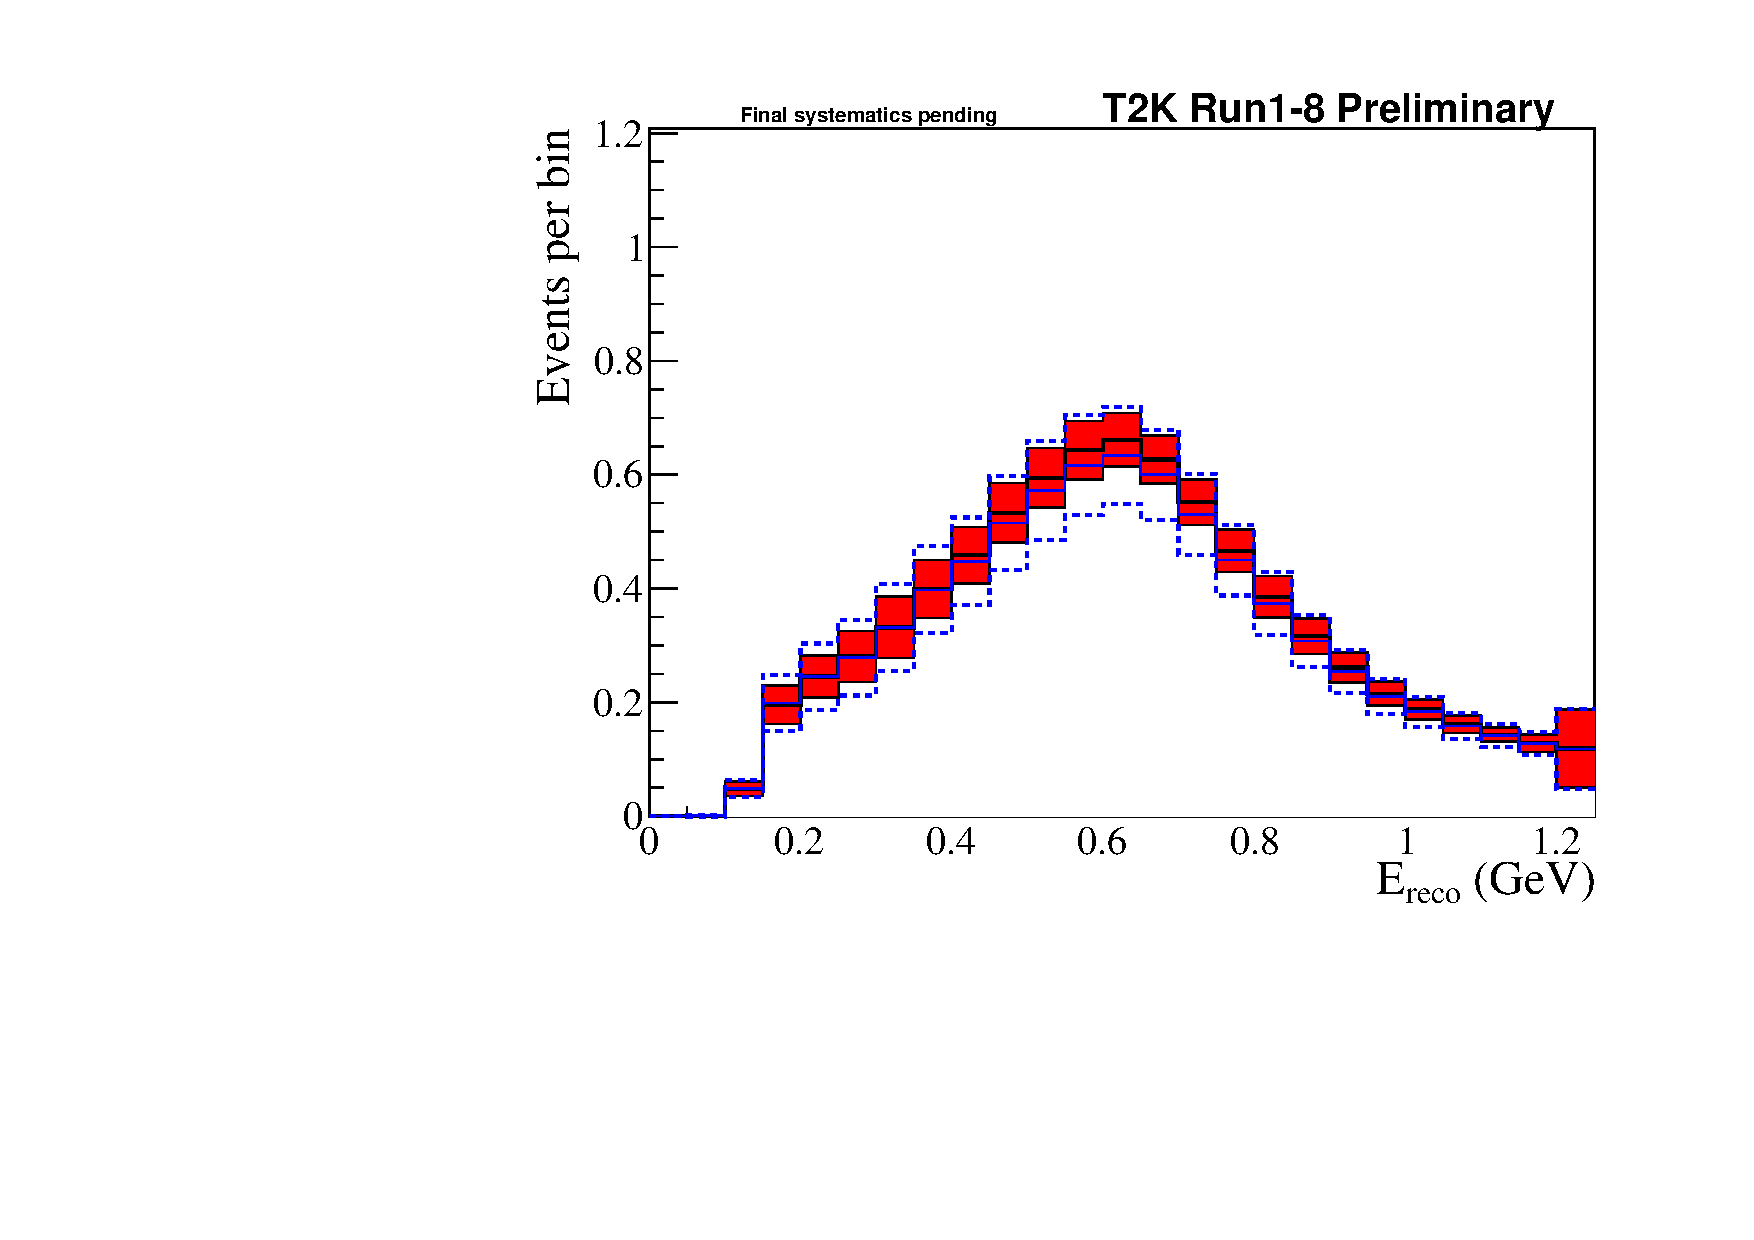
\includegraphics[width=0.9\textwidth]{systematics/envelopes/sk_errors/sk_error_table_RHC1Re_all_envelope}
		\caption{Electron-like antineutrino mode}
	\end{subfigure}
	\begin{subfigure}[b]{0.49\textwidth}
		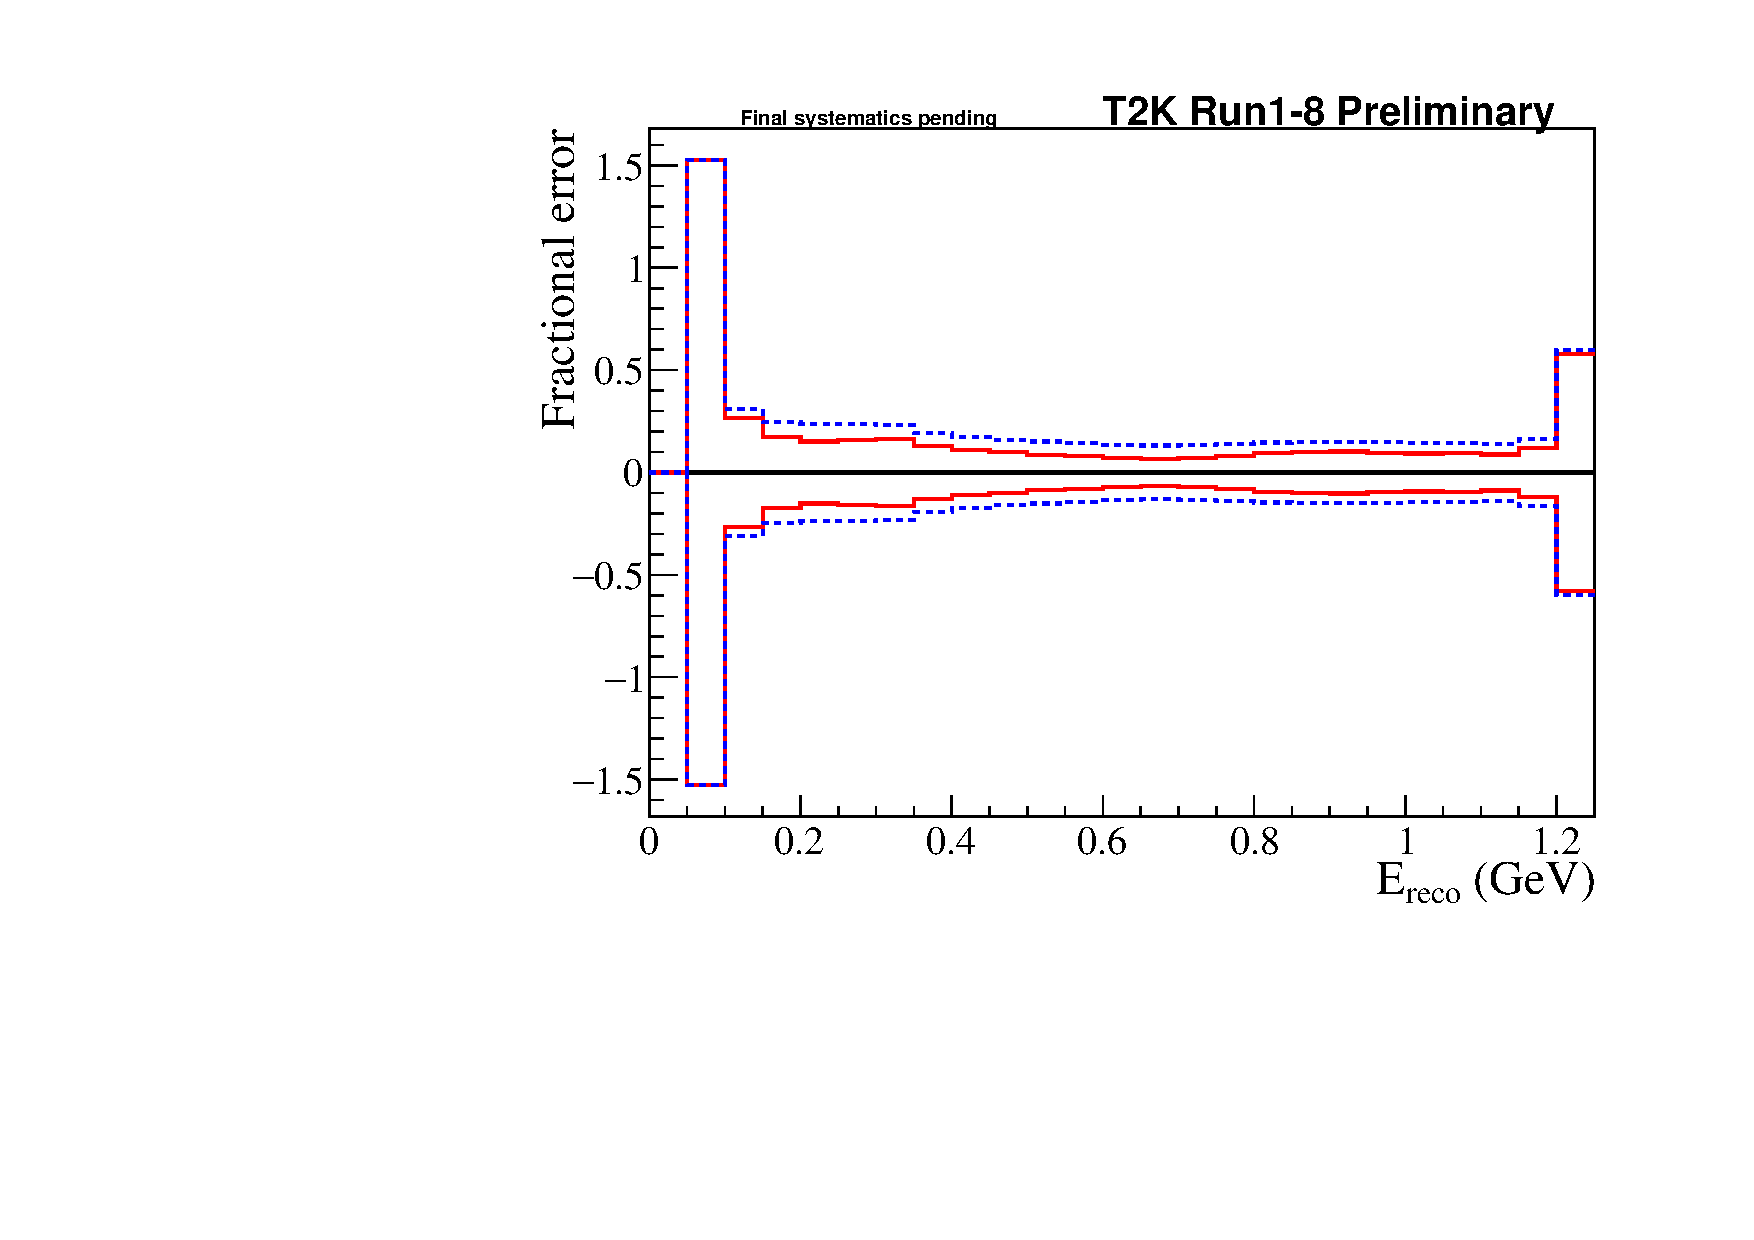
\includegraphics[width=0.9\textwidth]{systematics/envelopes/sk_errors/sk_error_table_RHC1Re_all_envelope_fractional}
		\caption{Electron-like antineutrino mode}
	\end{subfigure}
	\caption {
		Error envelopes (left) and fractional errors (right) for the reconstructed neutrino energy spectrum for all systematic parameters for pre-BANFF (blue) and post-BANFF (red) errors. \num{1e4} toys are generated for the Asimov data set A with randomized systematic parameters with correlations taken into account. Since \deltacp, \ssqthtwothree, \dmsqtwothree and the mass hierarchy will be measured, only the uncertainty on \ssqthonethree, \ssqthonetwo and \dmsqonetwo are taken into account.
	}
	\label{fig:sk_envelopes_all_b}
\end{figure*}
\clearpage
\begin{figure*}
	\center
	\begin{subfigure}[b]{0.49\textwidth}
		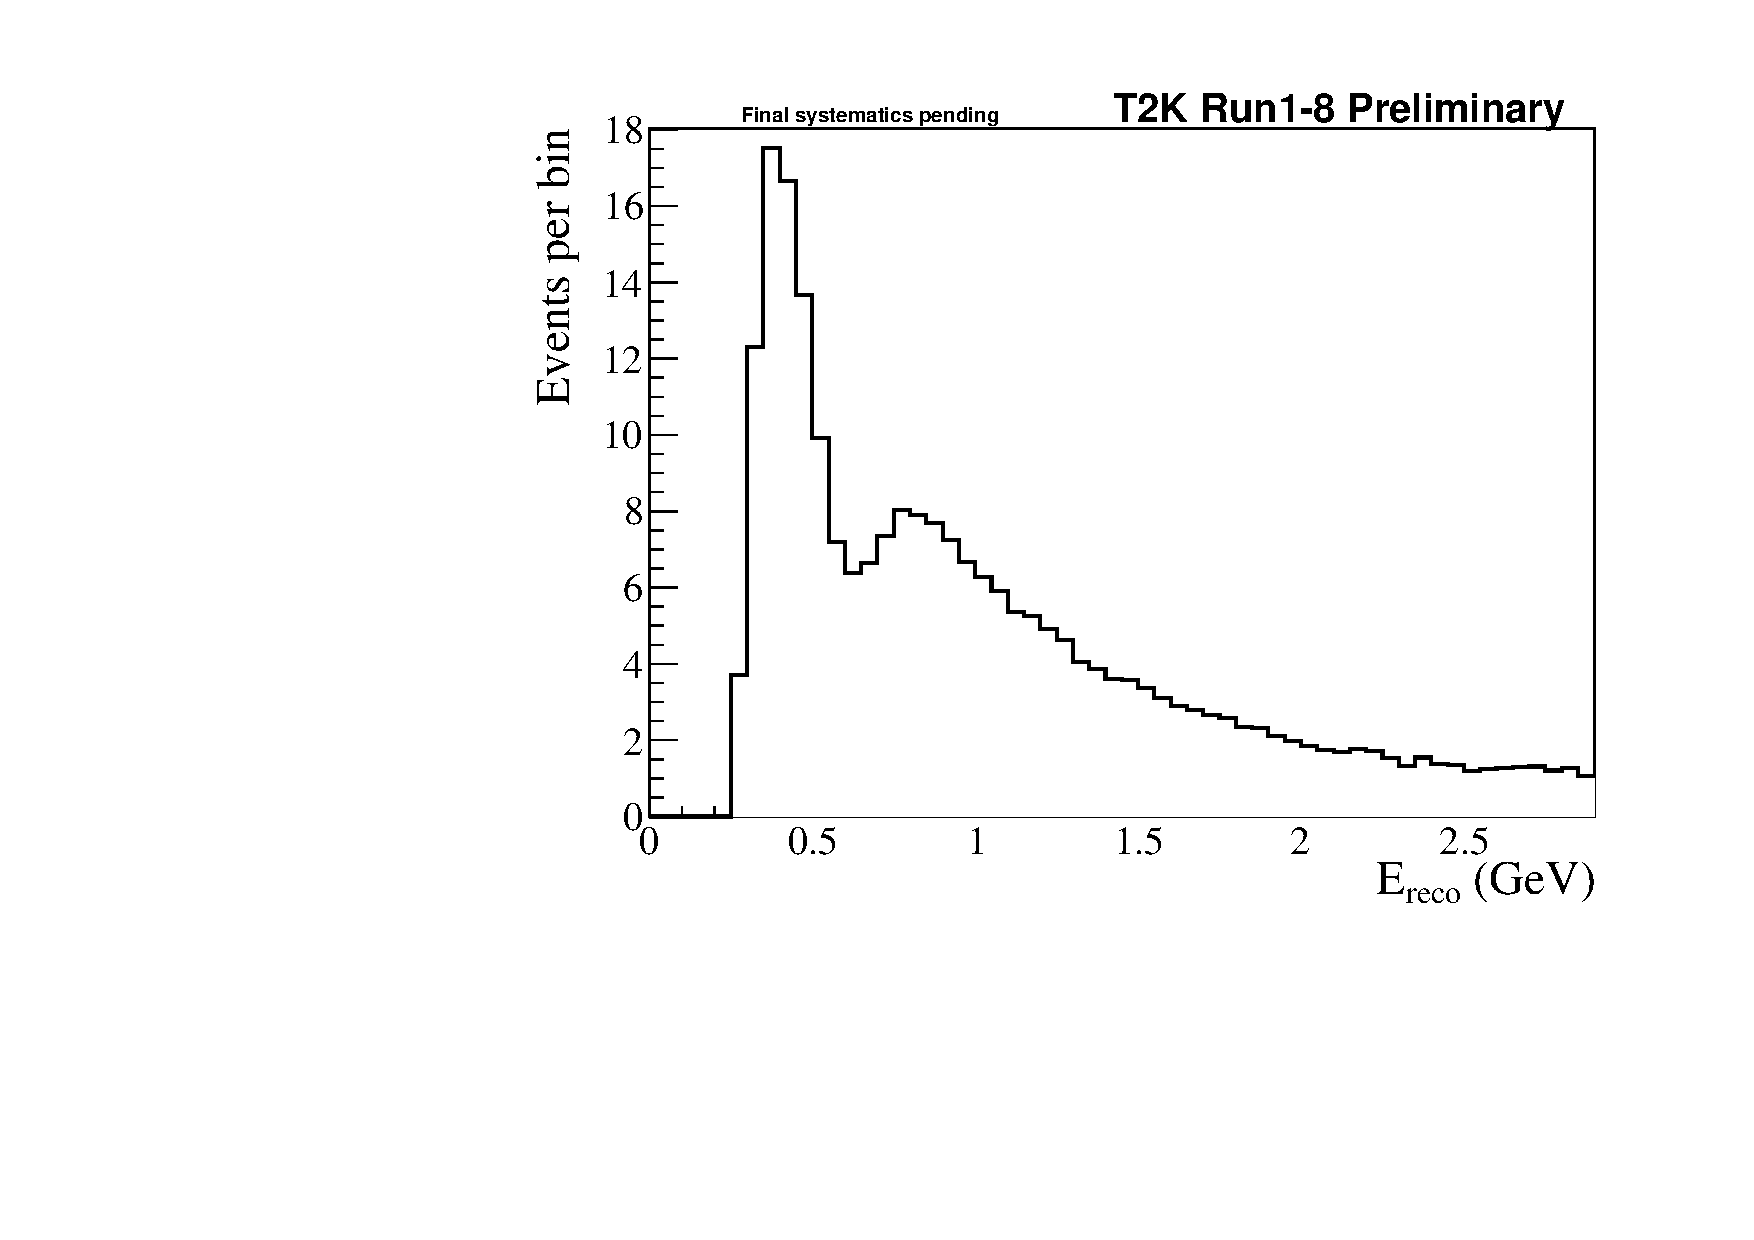
\includegraphics[width=0.9\textwidth]{systematics/envelopes/sk_errors/sk_error_table_1Rmu_osc_envelope}
		\caption{Muon-like, neutrino mode}
	\end{subfigure}
	\begin{subfigure}[b]{0.49\textwidth}
		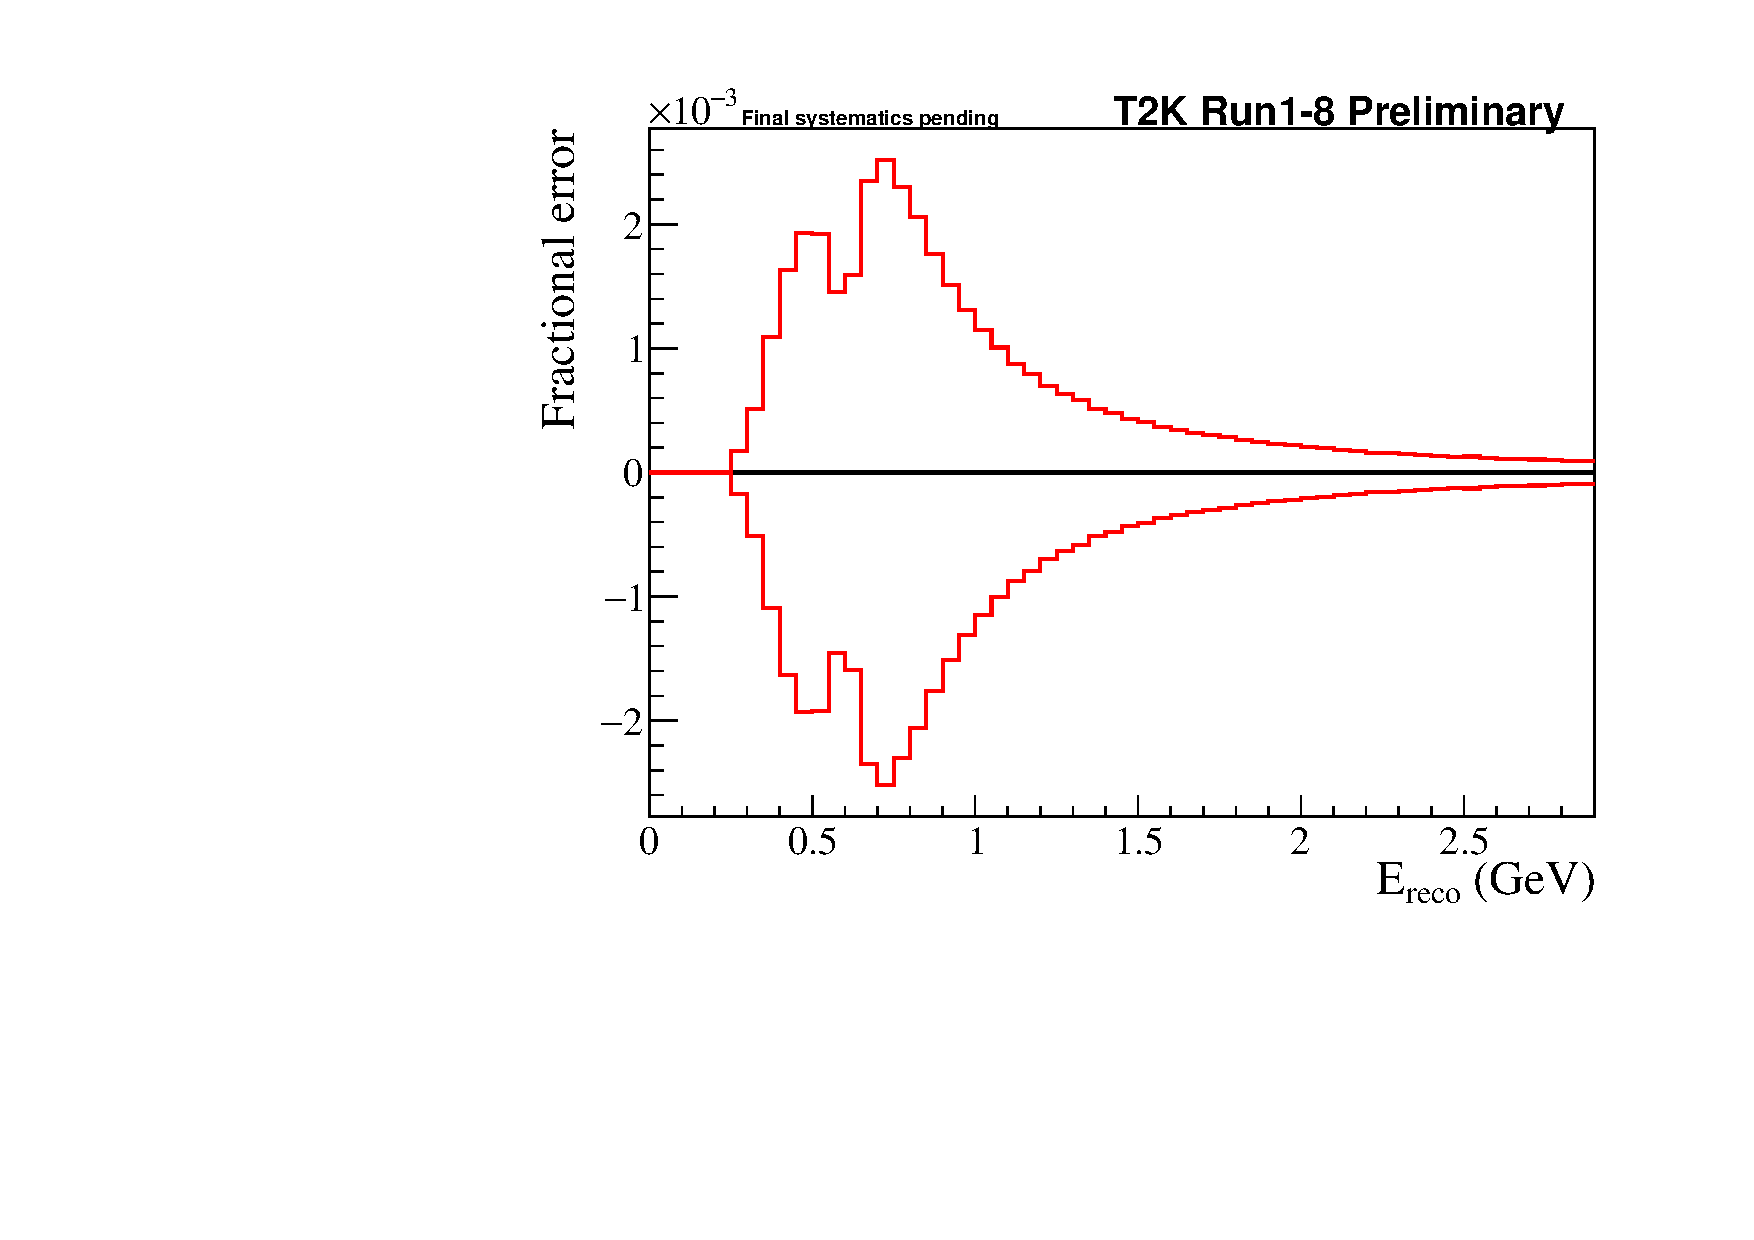
\includegraphics[width=0.9\textwidth]{systematics/envelopes/sk_errors/sk_error_table_1Rmu_osc_envelope_fractional}
		\caption{Muon-like, neutrino mode}
	\end{subfigure}
	\begin{subfigure}[b]{0.49\textwidth}
		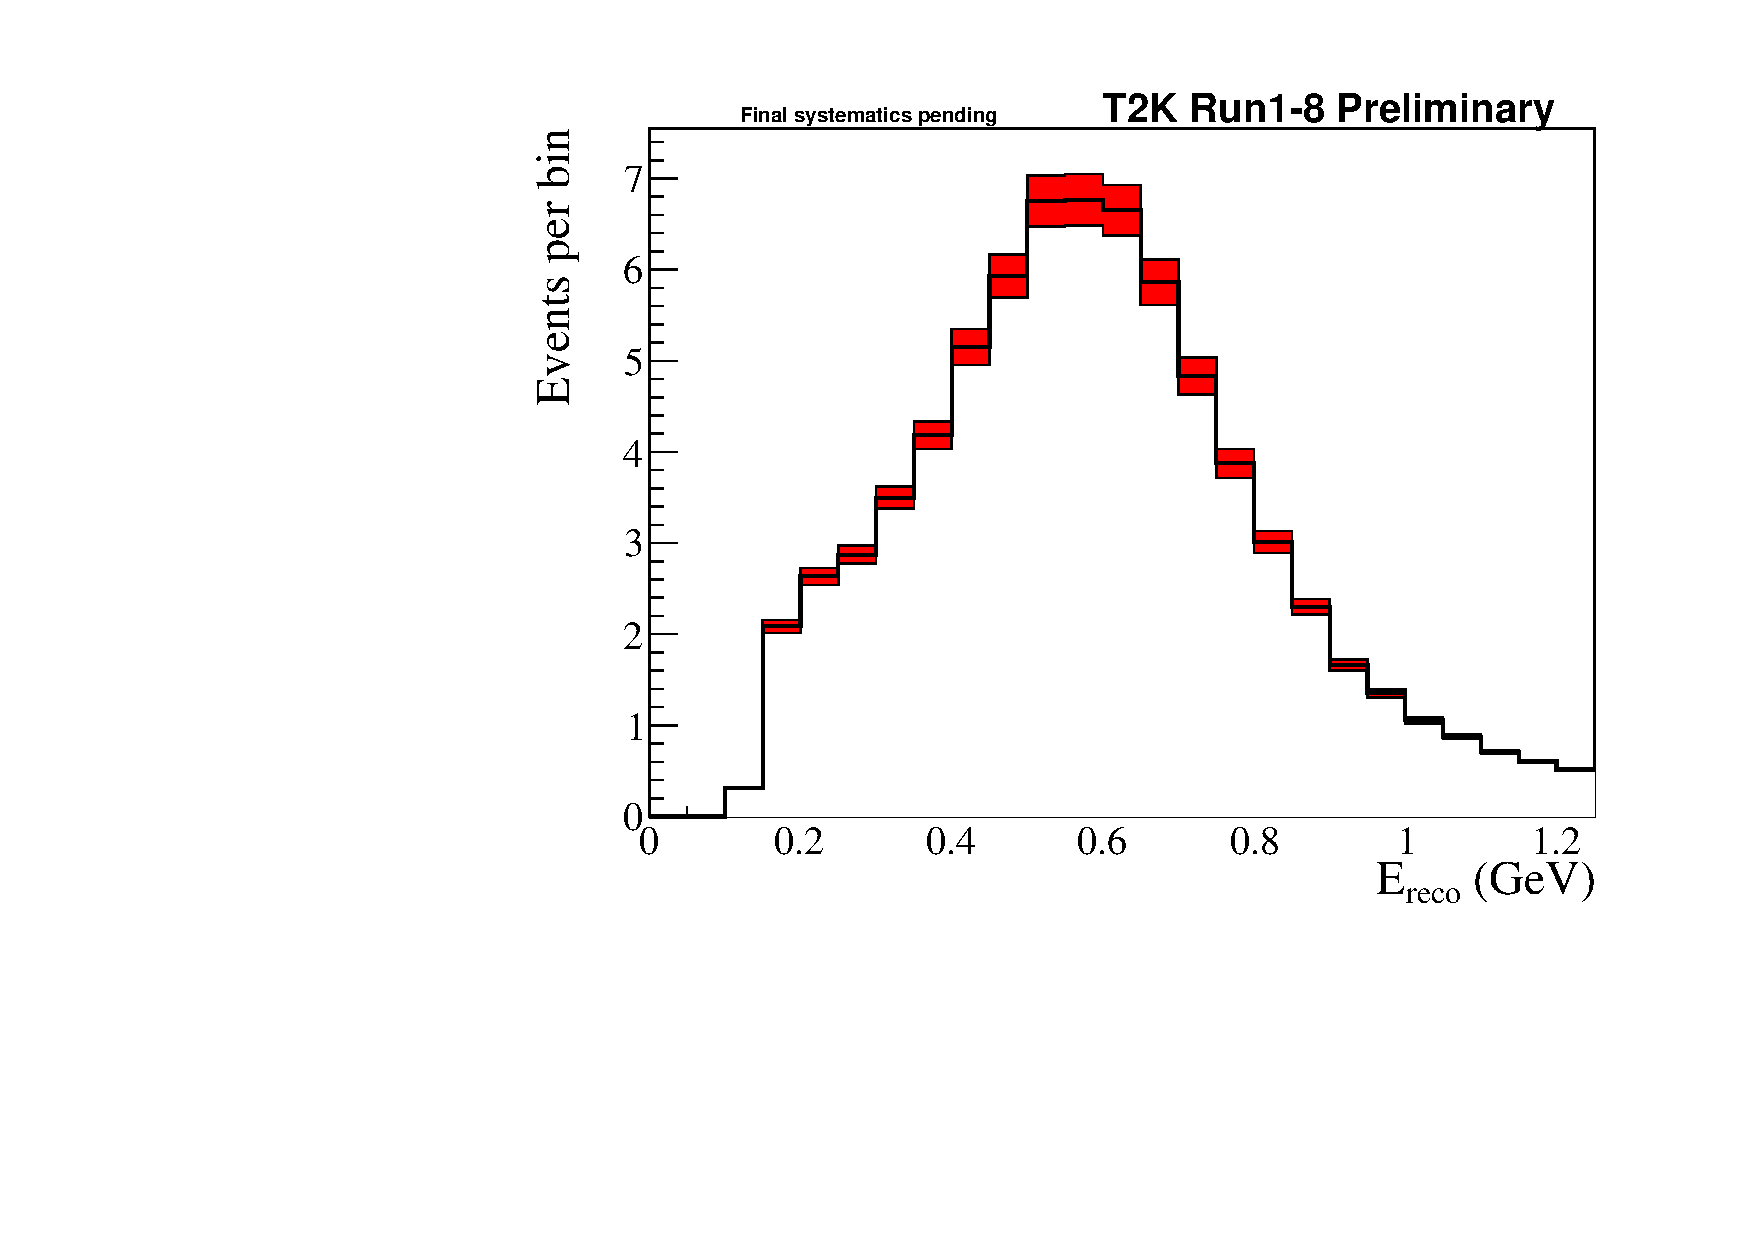
\includegraphics[width=0.9\textwidth]{systematics/envelopes/sk_errors/sk_error_table_1Re_osc_envelope}
		\caption{Electron-like, neutrino mode}
	\end{subfigure}
	\begin{subfigure}[b]{0.49\textwidth}
		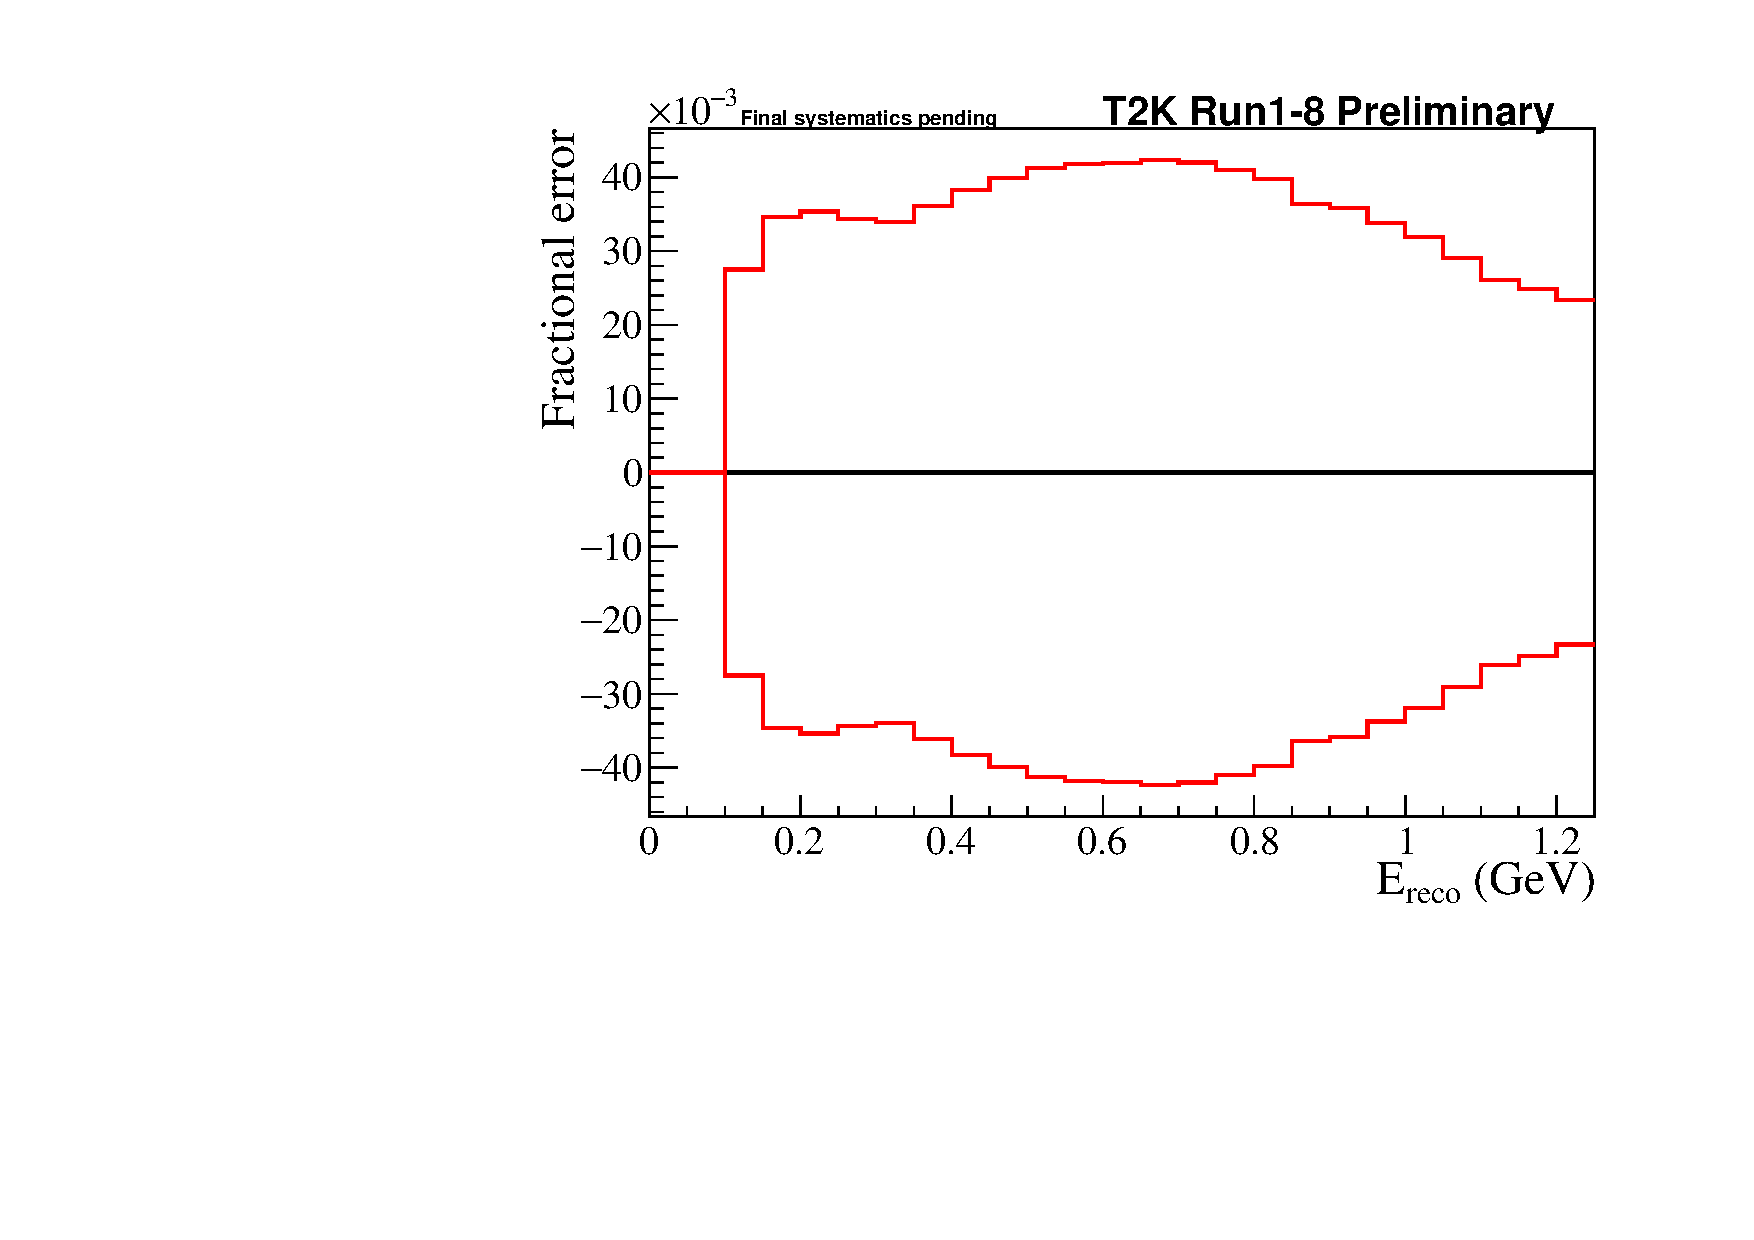
\includegraphics[width=0.9\textwidth]{systematics/envelopes/sk_errors/sk_error_table_1Re_osc_envelope_fractional}
		\caption{Electron-like, neutrino mode}
	\end{subfigure}
	\begin{subfigure}[b]{0.49\textwidth}
		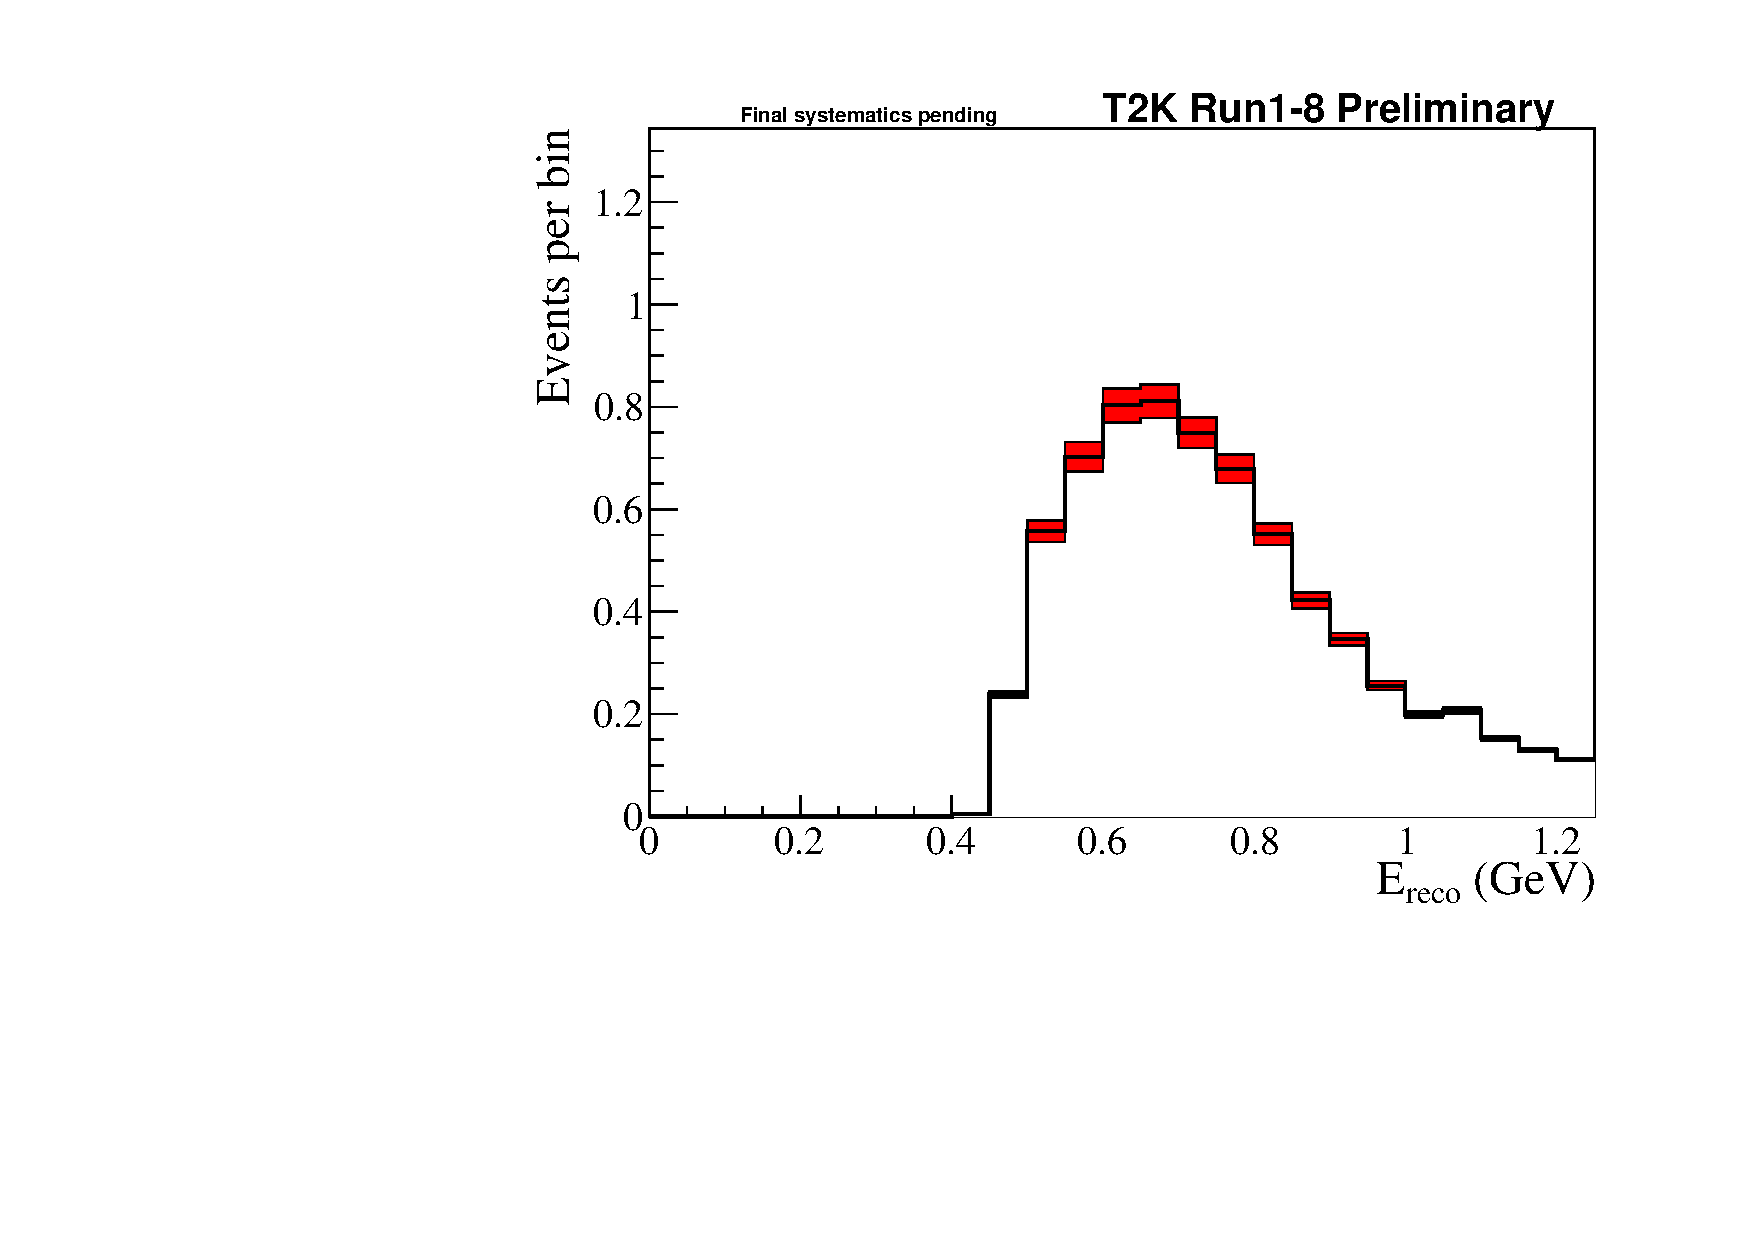
\includegraphics[width=0.9\textwidth]{systematics/envelopes/sk_errors/sk_error_table_MultiRe_osc_envelope}
		\caption{\nueCConepi-like, neutrino mode}
	\end{subfigure}
	\begin{subfigure}[b]{0.49\textwidth}
		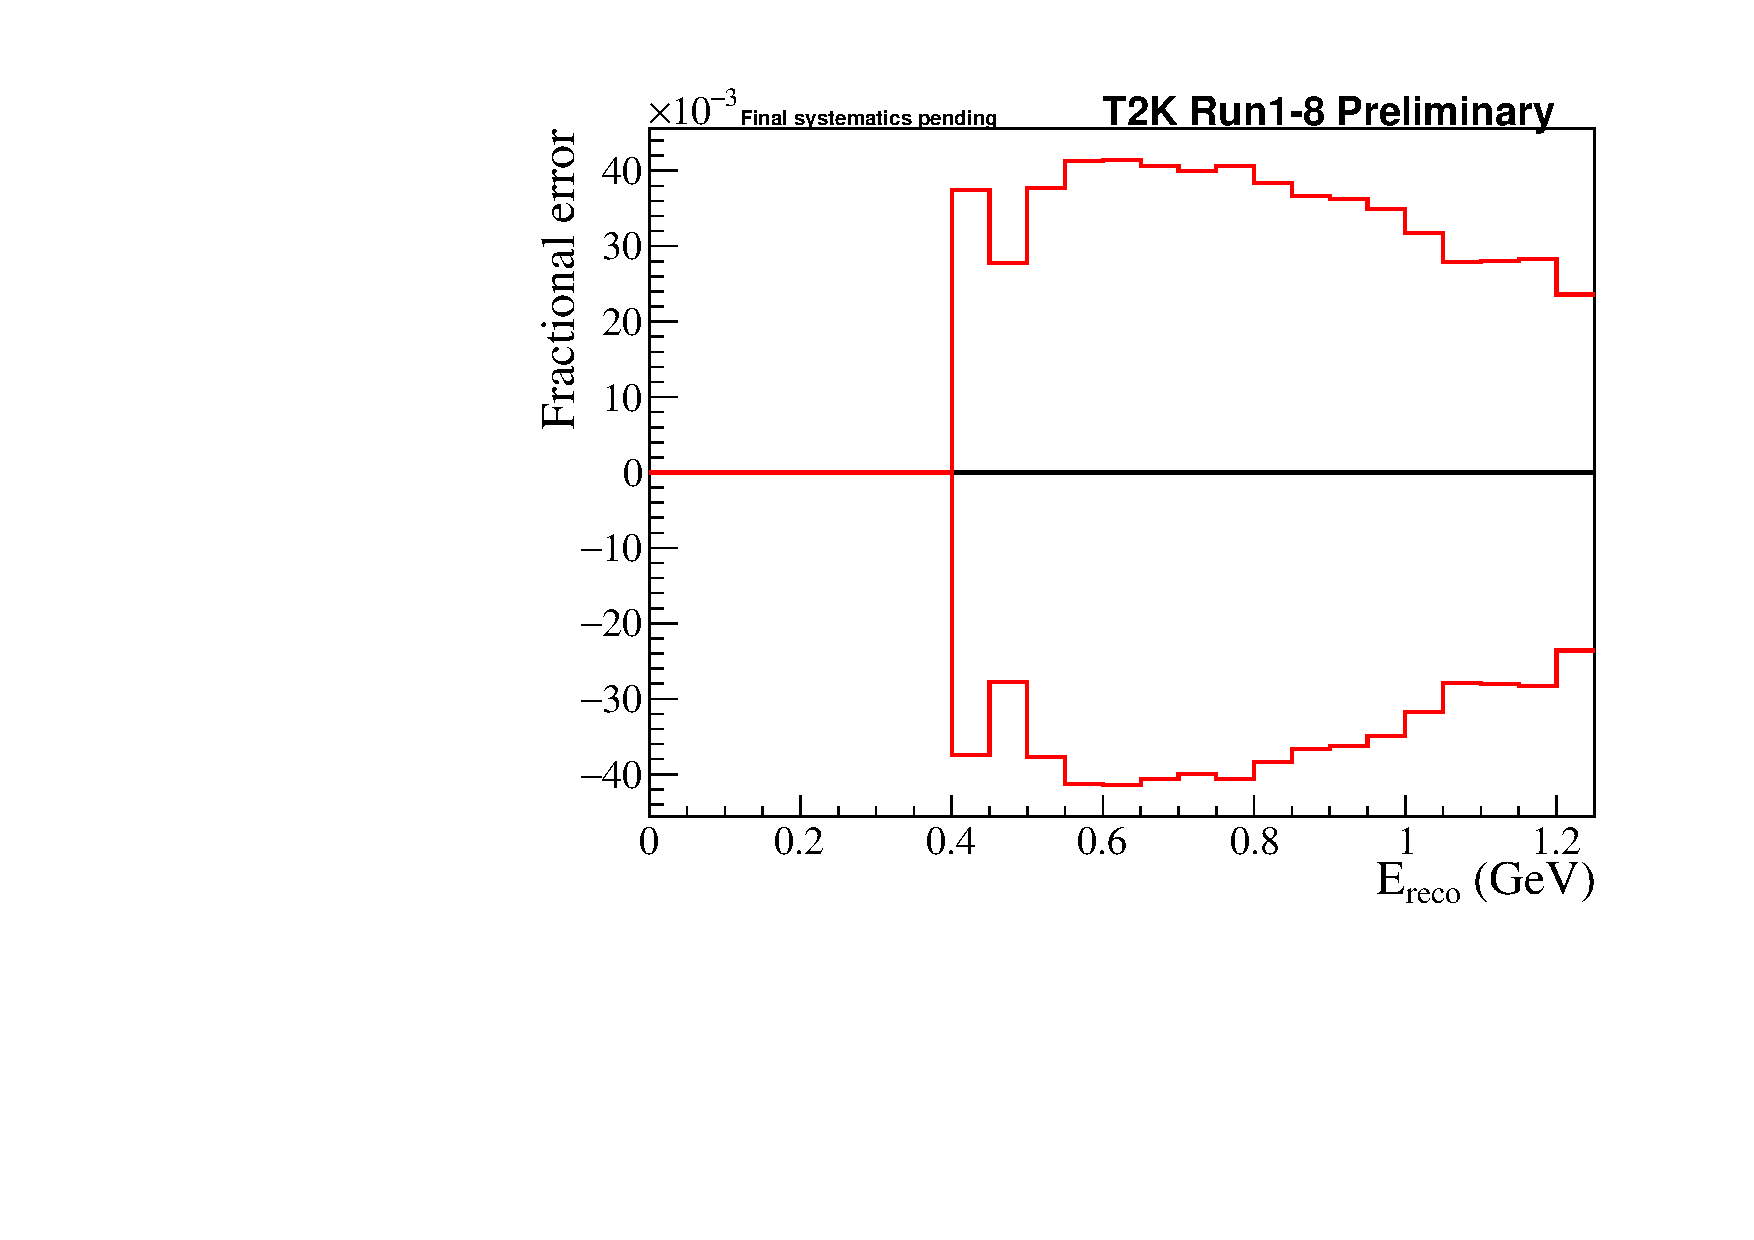
\includegraphics[width=0.9\textwidth]{systematics/envelopes/sk_errors/sk_error_table_MultiRe_osc_envelope_fractional}
		\caption{\nueCConepi-like, neutrino mode}
	\end{subfigure}
	\caption {
		Error envelopes (left) and fractional errors (right) for the reconstructed neutrino energy spectrum for all oscillation nuisance parameters. \num{1e4} toys are generated for the Asimov data set A with randomized systematic parameters with correlations taken into account. Since \deltacp, \ssqthtwothree, \dmsqtwothree and the mass hierarchy will be measured, only the uncertainty on \ssqthonethree, \ssqthonetwo and \dmsqonetwo are taken into account.
	}
	\label{fig:sk_envelopes_osc}
\end{figure*}
\clearpage

\begin{figure*}
	\center
	\begin{subfigure}[b]{0.49\textwidth}
		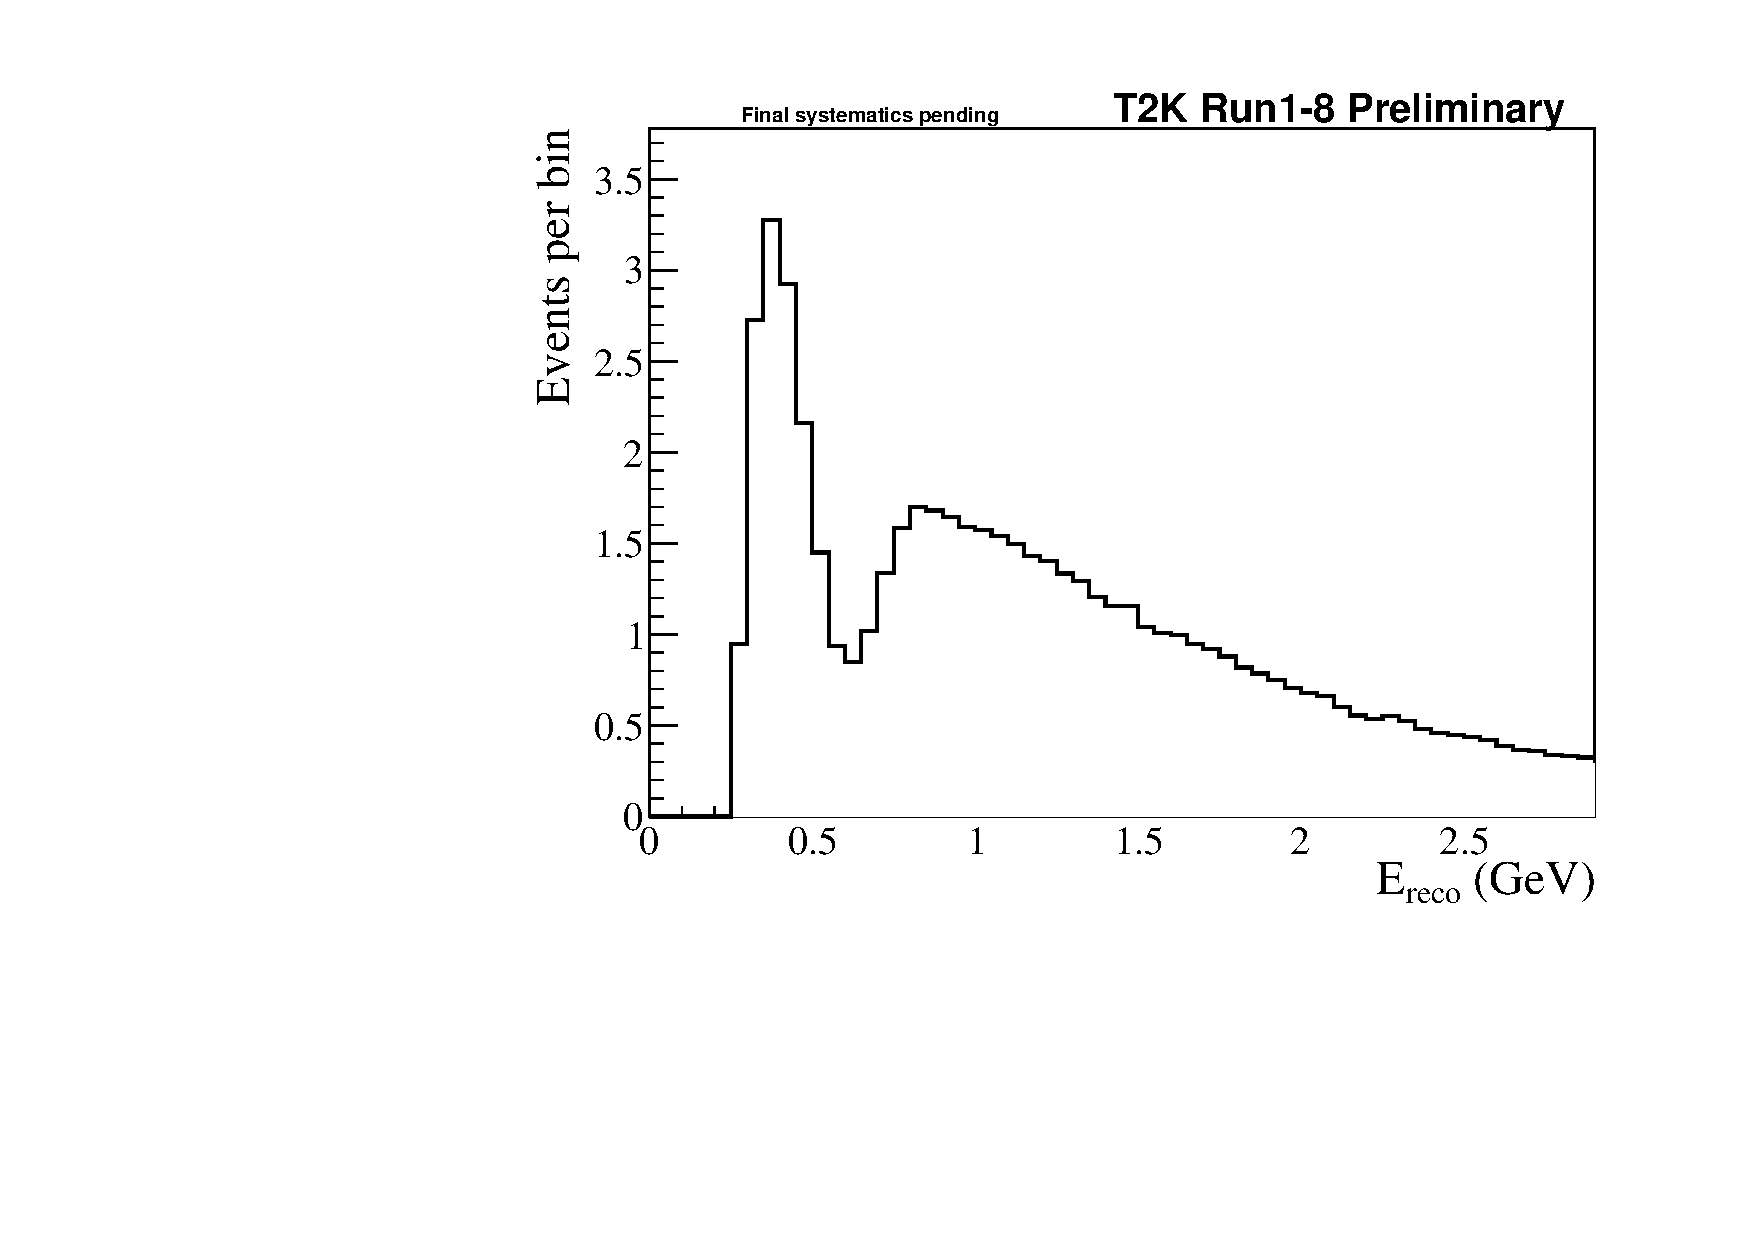
\includegraphics[width=0.9\textwidth]{systematics/envelopes/sk_errors/sk_error_table_RHC1Rmu_osc_envelope}
		\caption{Muon-like, antineutrino mode}
	\end{subfigure}
	\begin{subfigure}[b]{0.49\textwidth}
		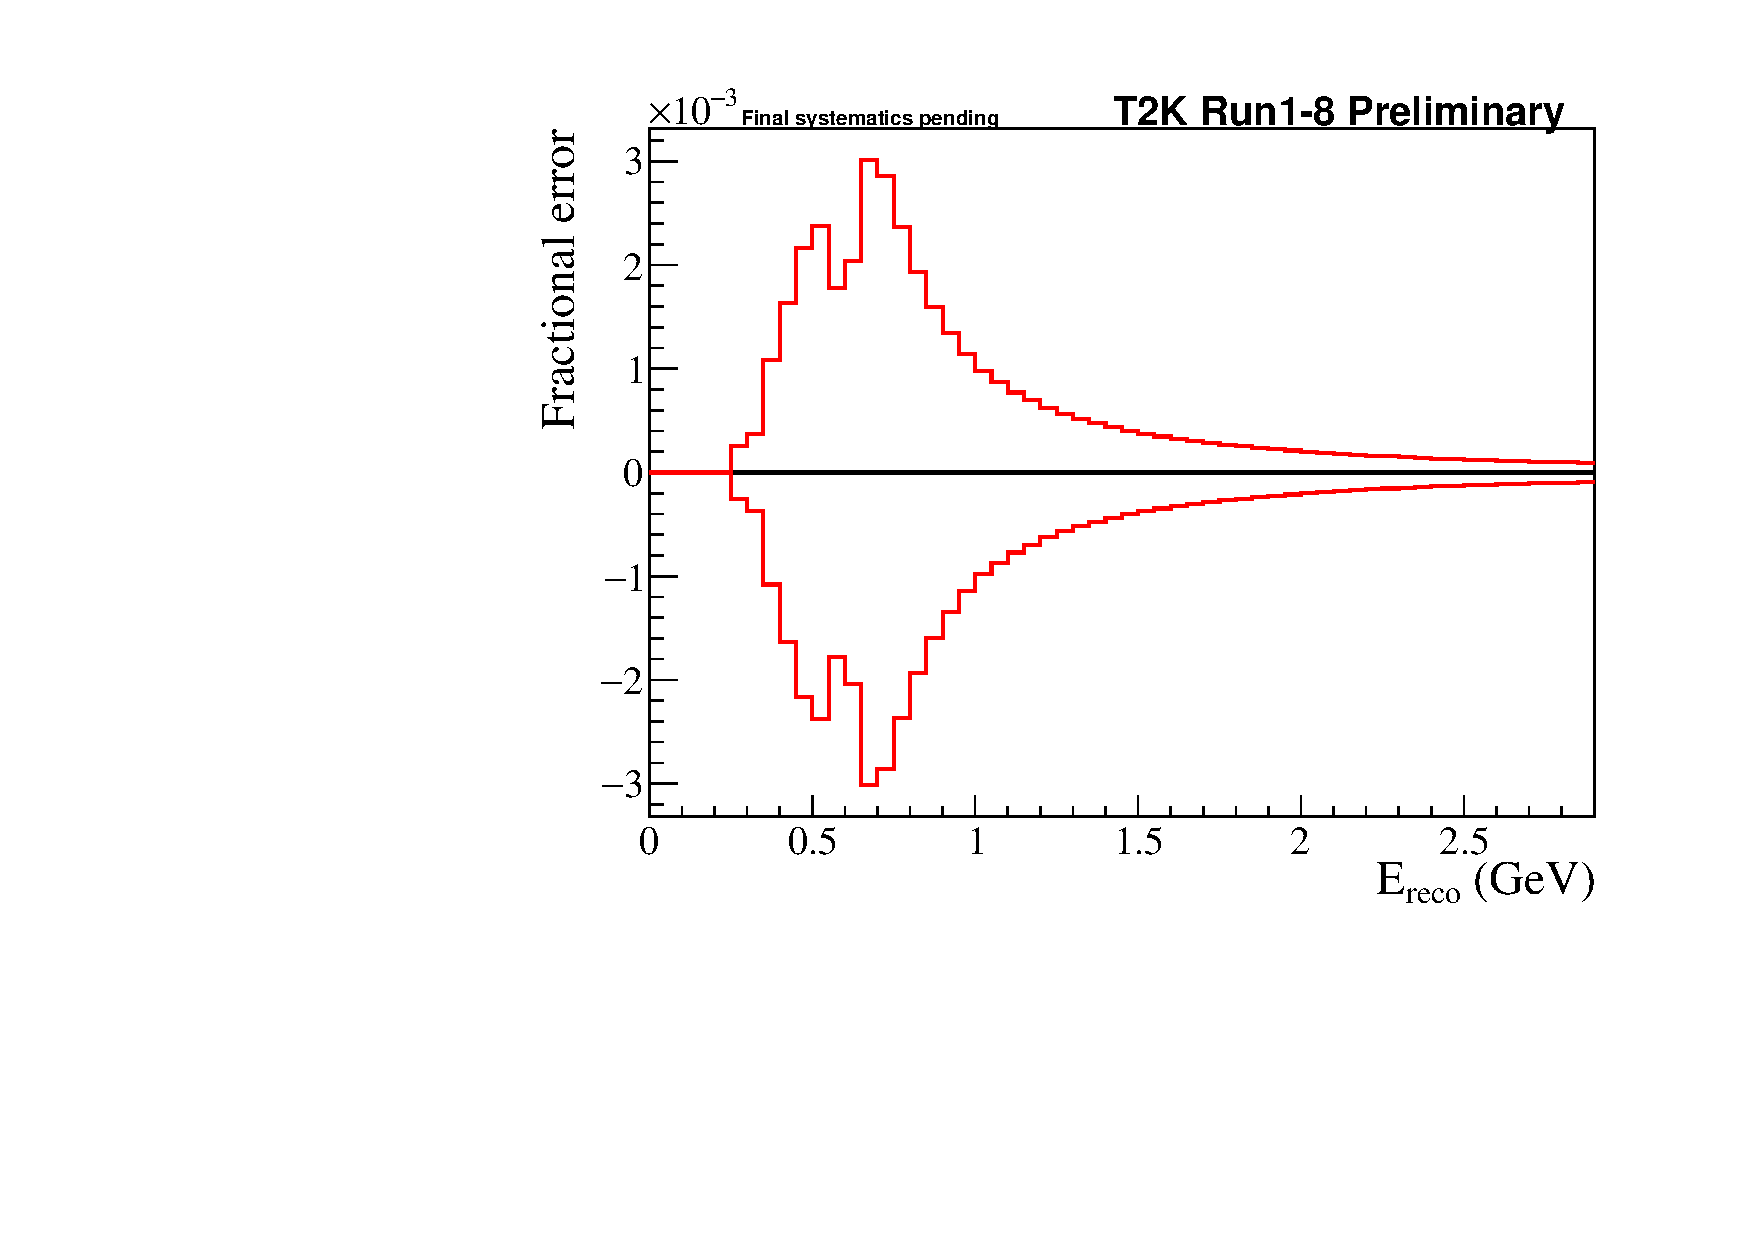
\includegraphics[width=0.9\textwidth]{systematics/envelopes/sk_errors/sk_error_table_RHC1Rmu_osc_envelope_fractional}
		\caption{Muon-like, antineutrino mode}
	\end{subfigure}
	\begin{subfigure}[b]{0.49\textwidth}
		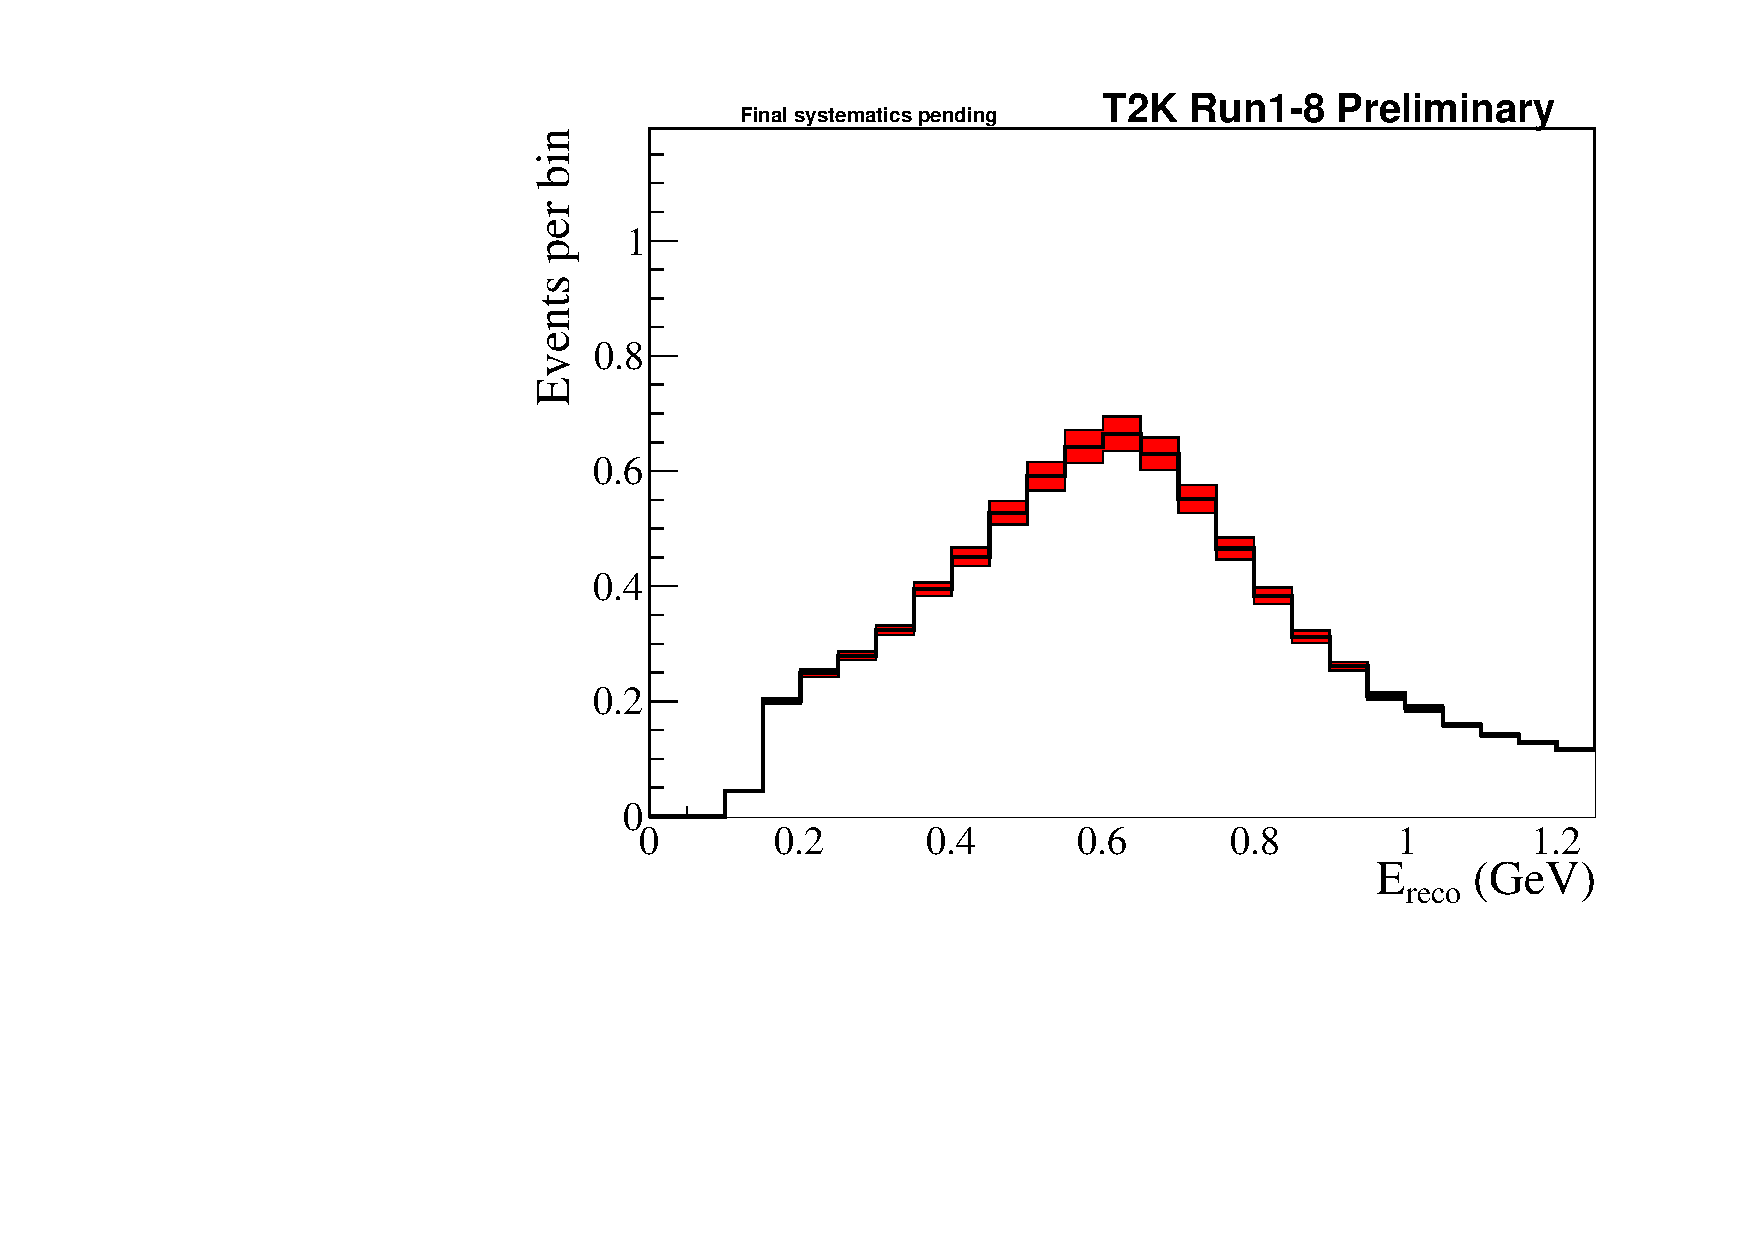
\includegraphics[width=0.9\textwidth]{systematics/envelopes/sk_errors/sk_error_table_RHC1Re_osc_envelope}
		\caption{Electron-like antineutrino mode}
	\end{subfigure}
	\begin{subfigure}[b]{0.49\textwidth}
		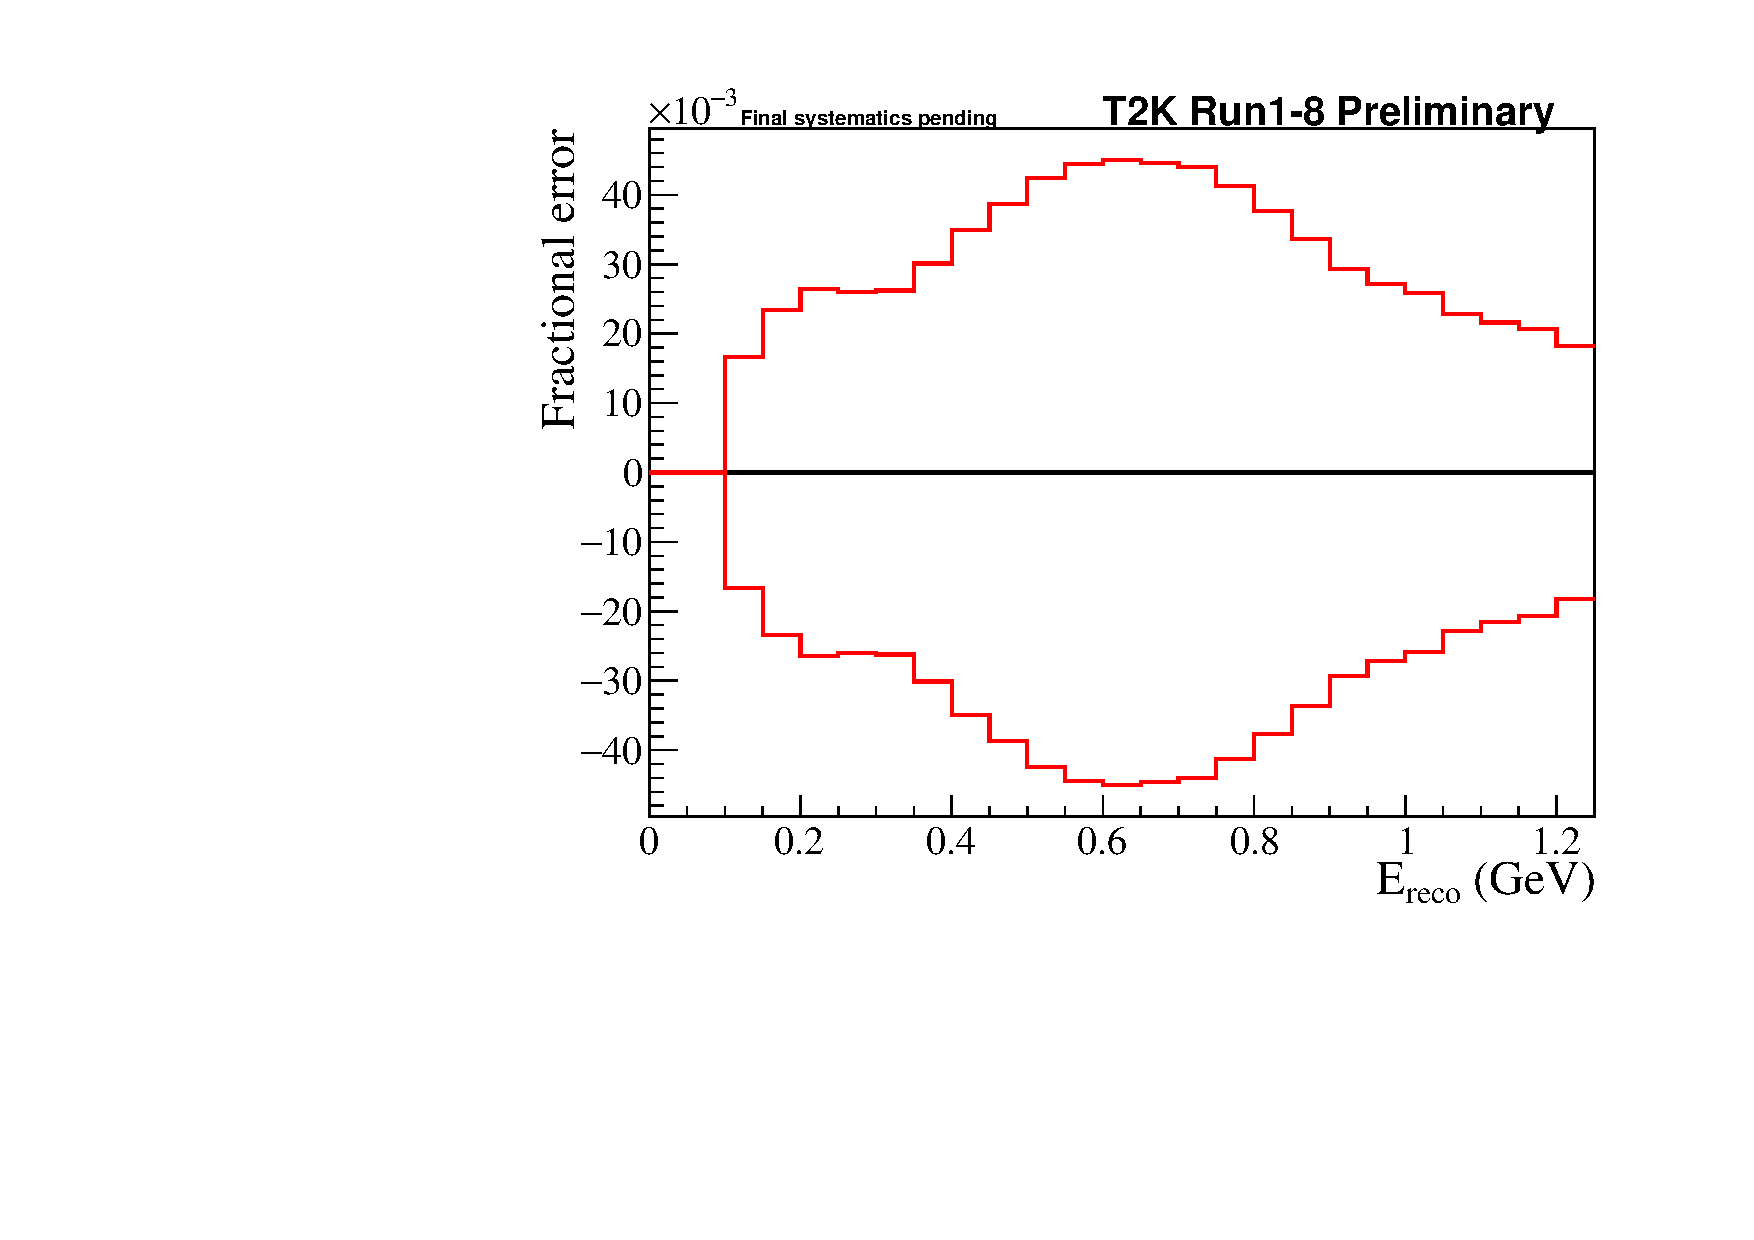
\includegraphics[width=0.9\textwidth]{systematics/envelopes/sk_errors/sk_error_table_RHC1Re_osc_envelope_fractional}
		\caption{Electron-like antineutrino mode}
	\end{subfigure}
	\caption {
		Error envelopes (left) and fractional errors (right) for the reconstructed neutrino energy spectrum for all oscillation nuisance parameters. \num{1e4} toys are generated for the Asimov data set A with randomized systematic parameters with correlations taken into account. Since \deltacp, \ssqthtwothree, \dmsqtwothree and the mass hierarchy will be measured, only the uncertainty on \ssqthonethree, \ssqthonetwo and \dmsqonetwo are taken into account.
	}
	\label{fig:sk_envelopes_osc_b}
\end{figure*}
\clearpage
\begin{figure*}
	\center
	\begin{subfigure}[b]{0.49\textwidth}
		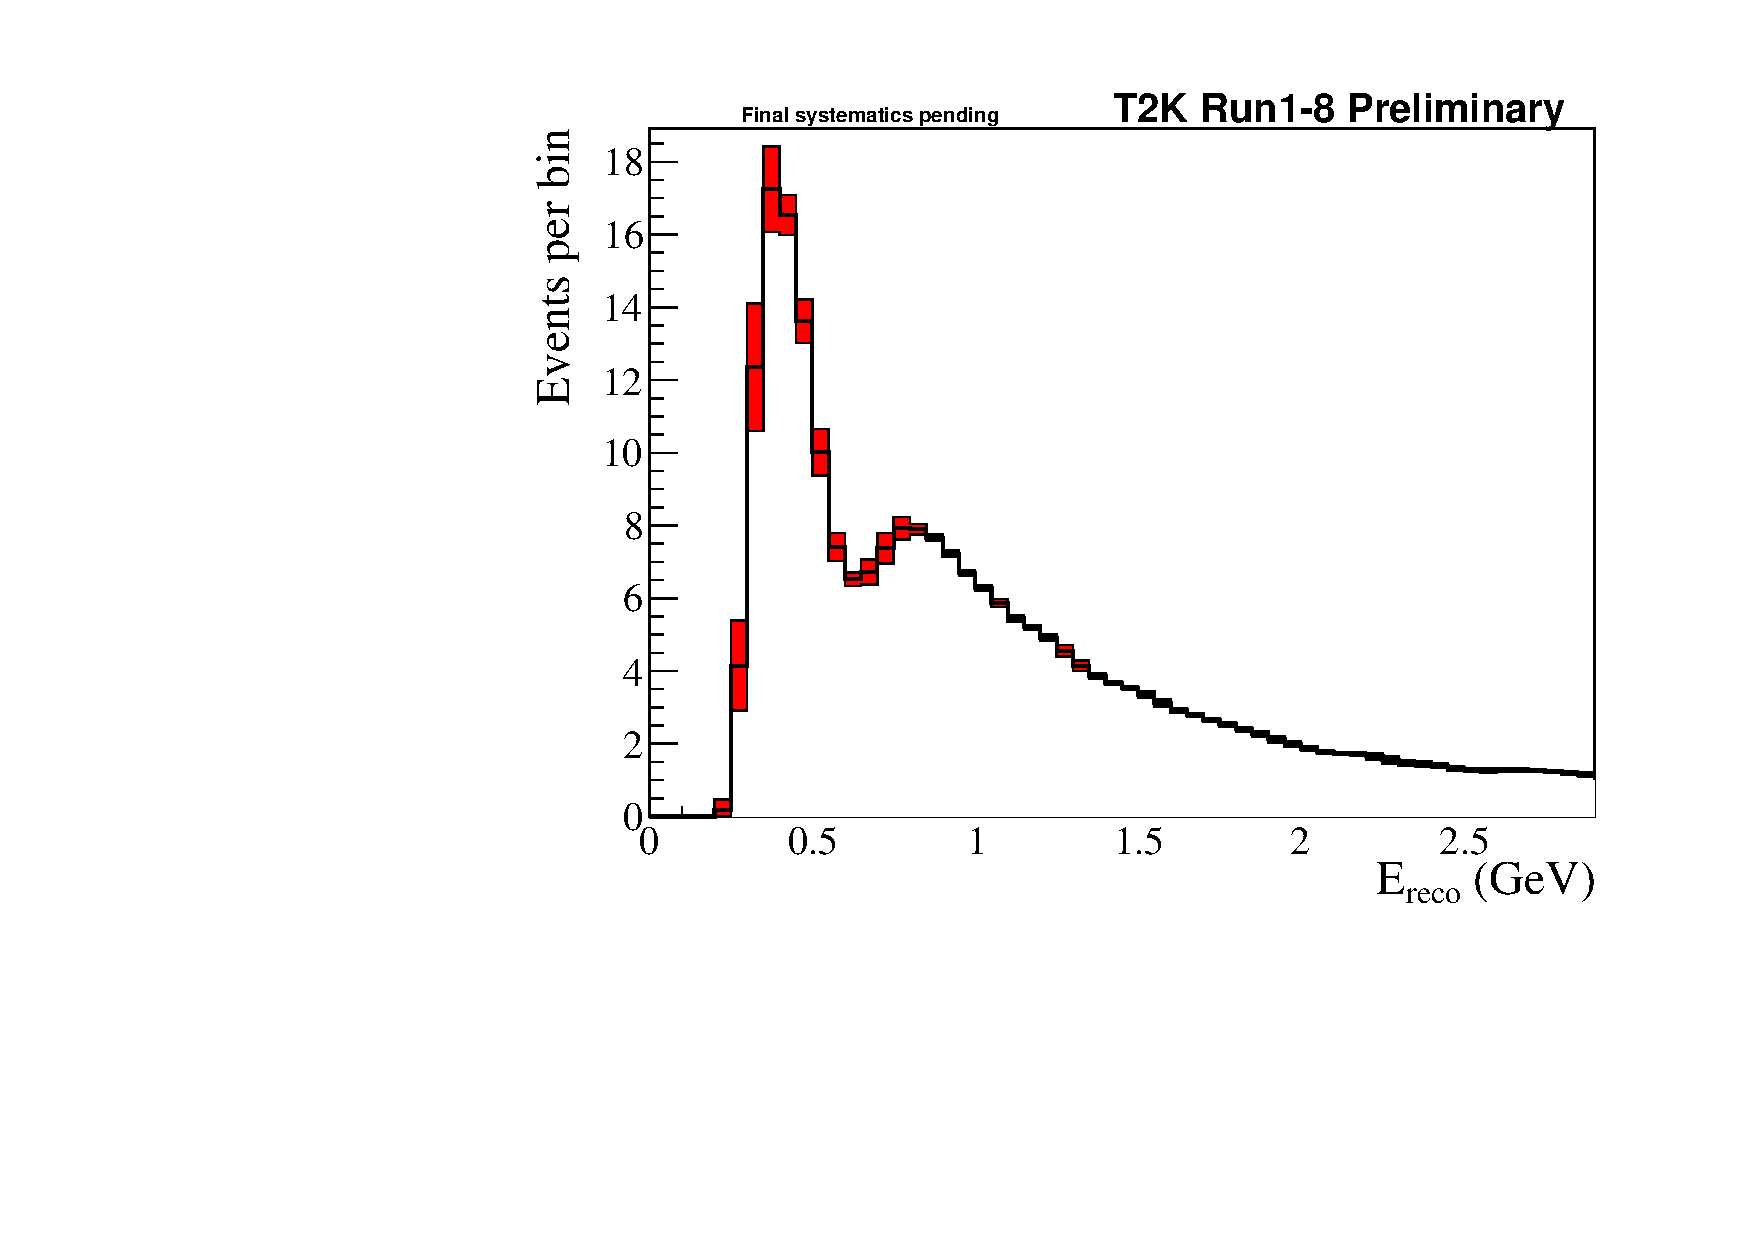
\includegraphics[width=0.9\textwidth]{systematics/envelopes/sk_errors/sk_error_table_1Rmu_skdet_envelope}
		\caption{Muon-like, neutrino mode}
	\end{subfigure}
	\begin{subfigure}[b]{0.49\textwidth}
		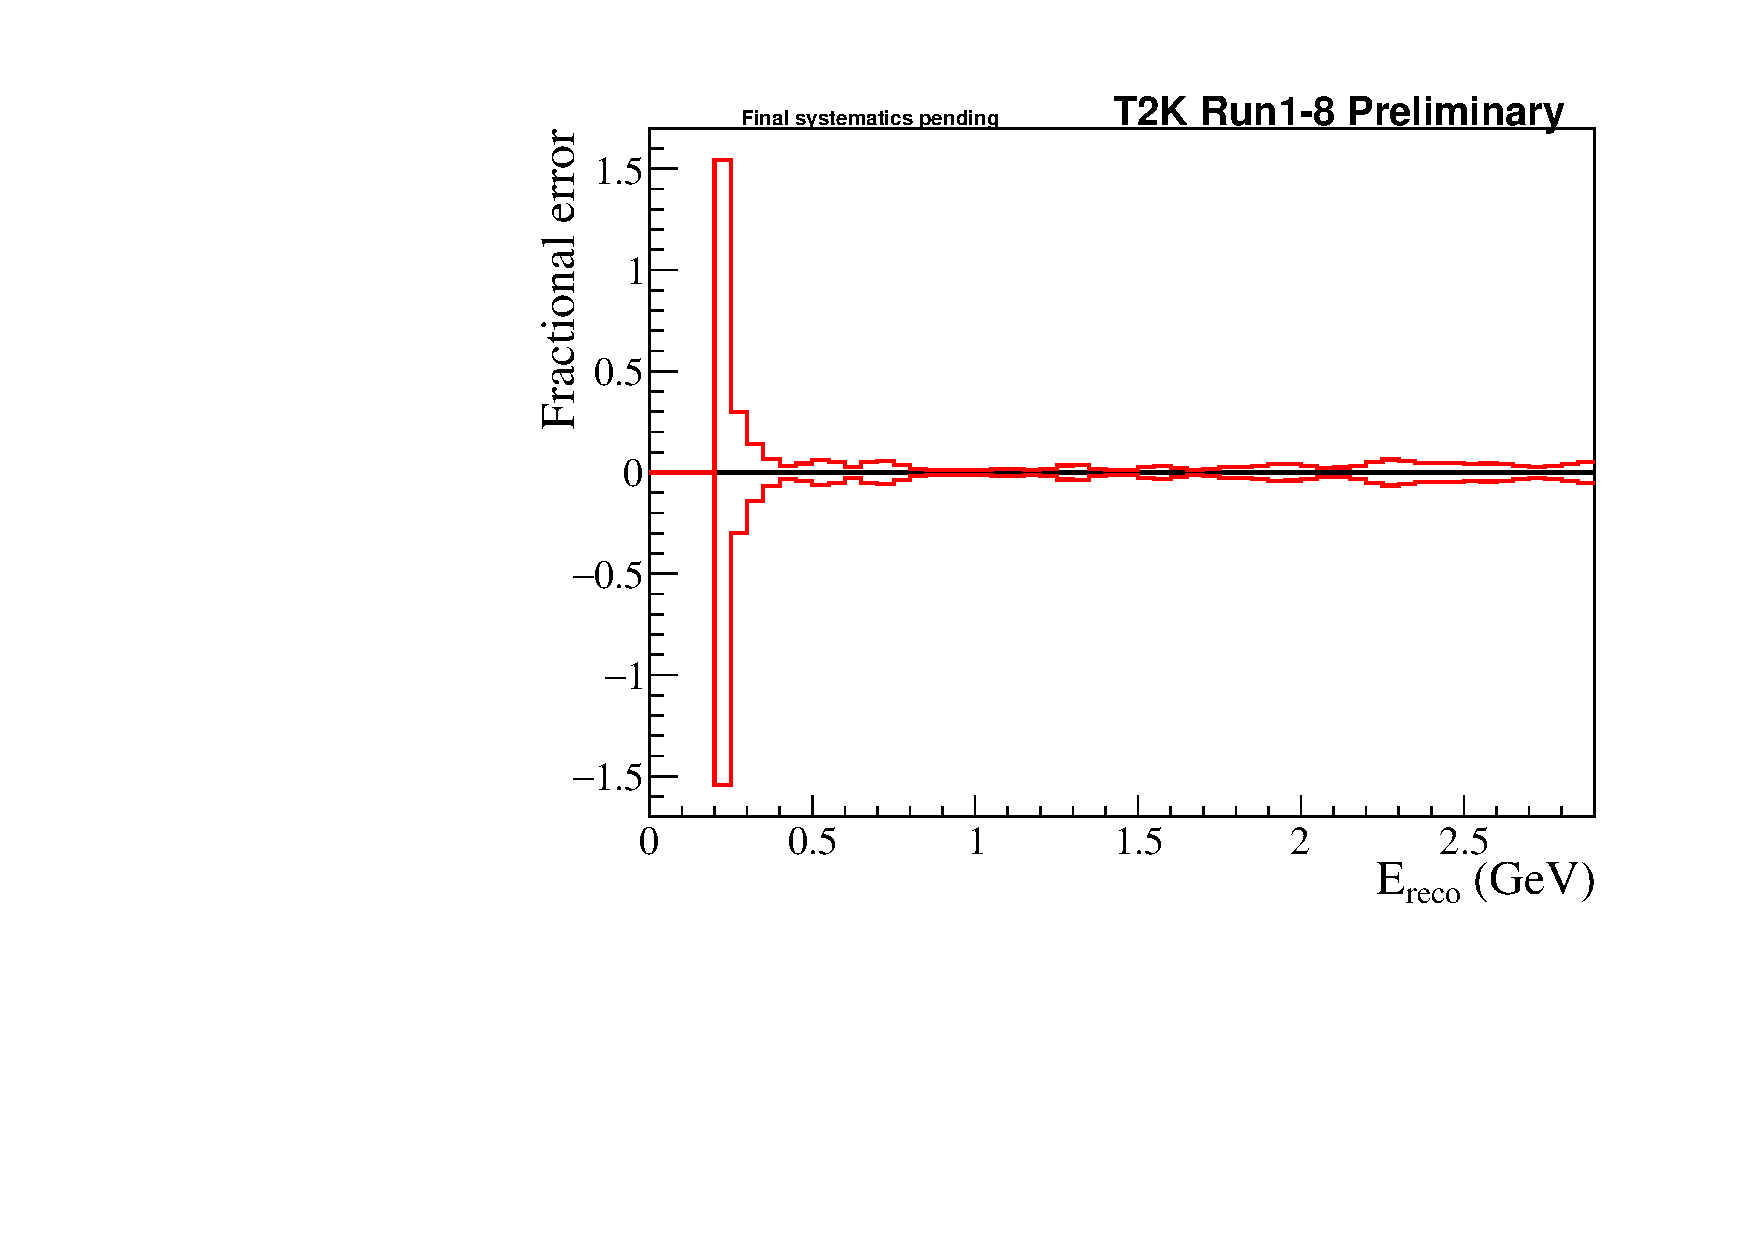
\includegraphics[width=0.9\textwidth]{systematics/envelopes/sk_errors/sk_error_table_1Rmu_skdet_envelope_fractional}
		\caption{Muon-like, neutrino mode}
	\end{subfigure}
	\begin{subfigure}[b]{0.49\textwidth}
		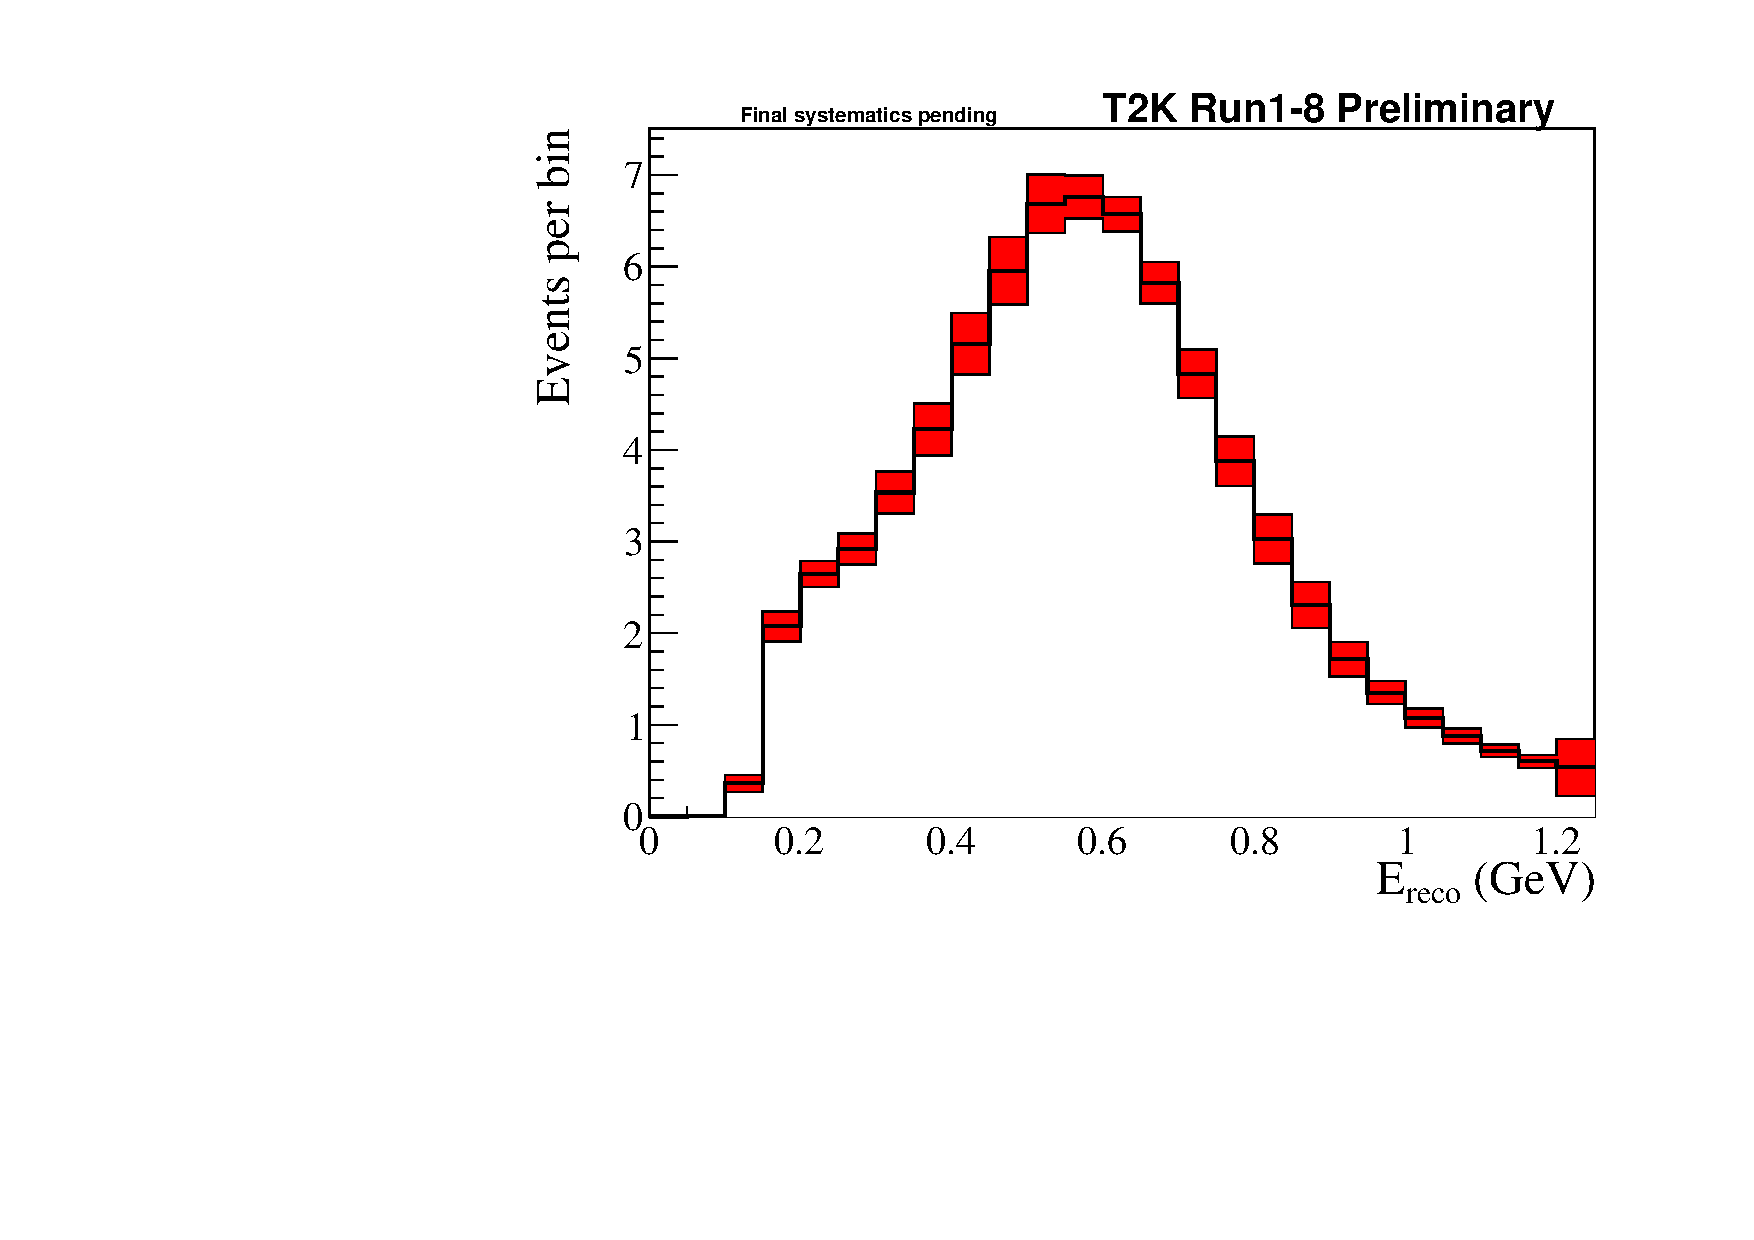
\includegraphics[width=0.9\textwidth]{systematics/envelopes/sk_errors/sk_error_table_1Re_skdet_envelope}
		\caption{Electron-like, neutrino mode}
	\end{subfigure}
	\begin{subfigure}[b]{0.49\textwidth}
		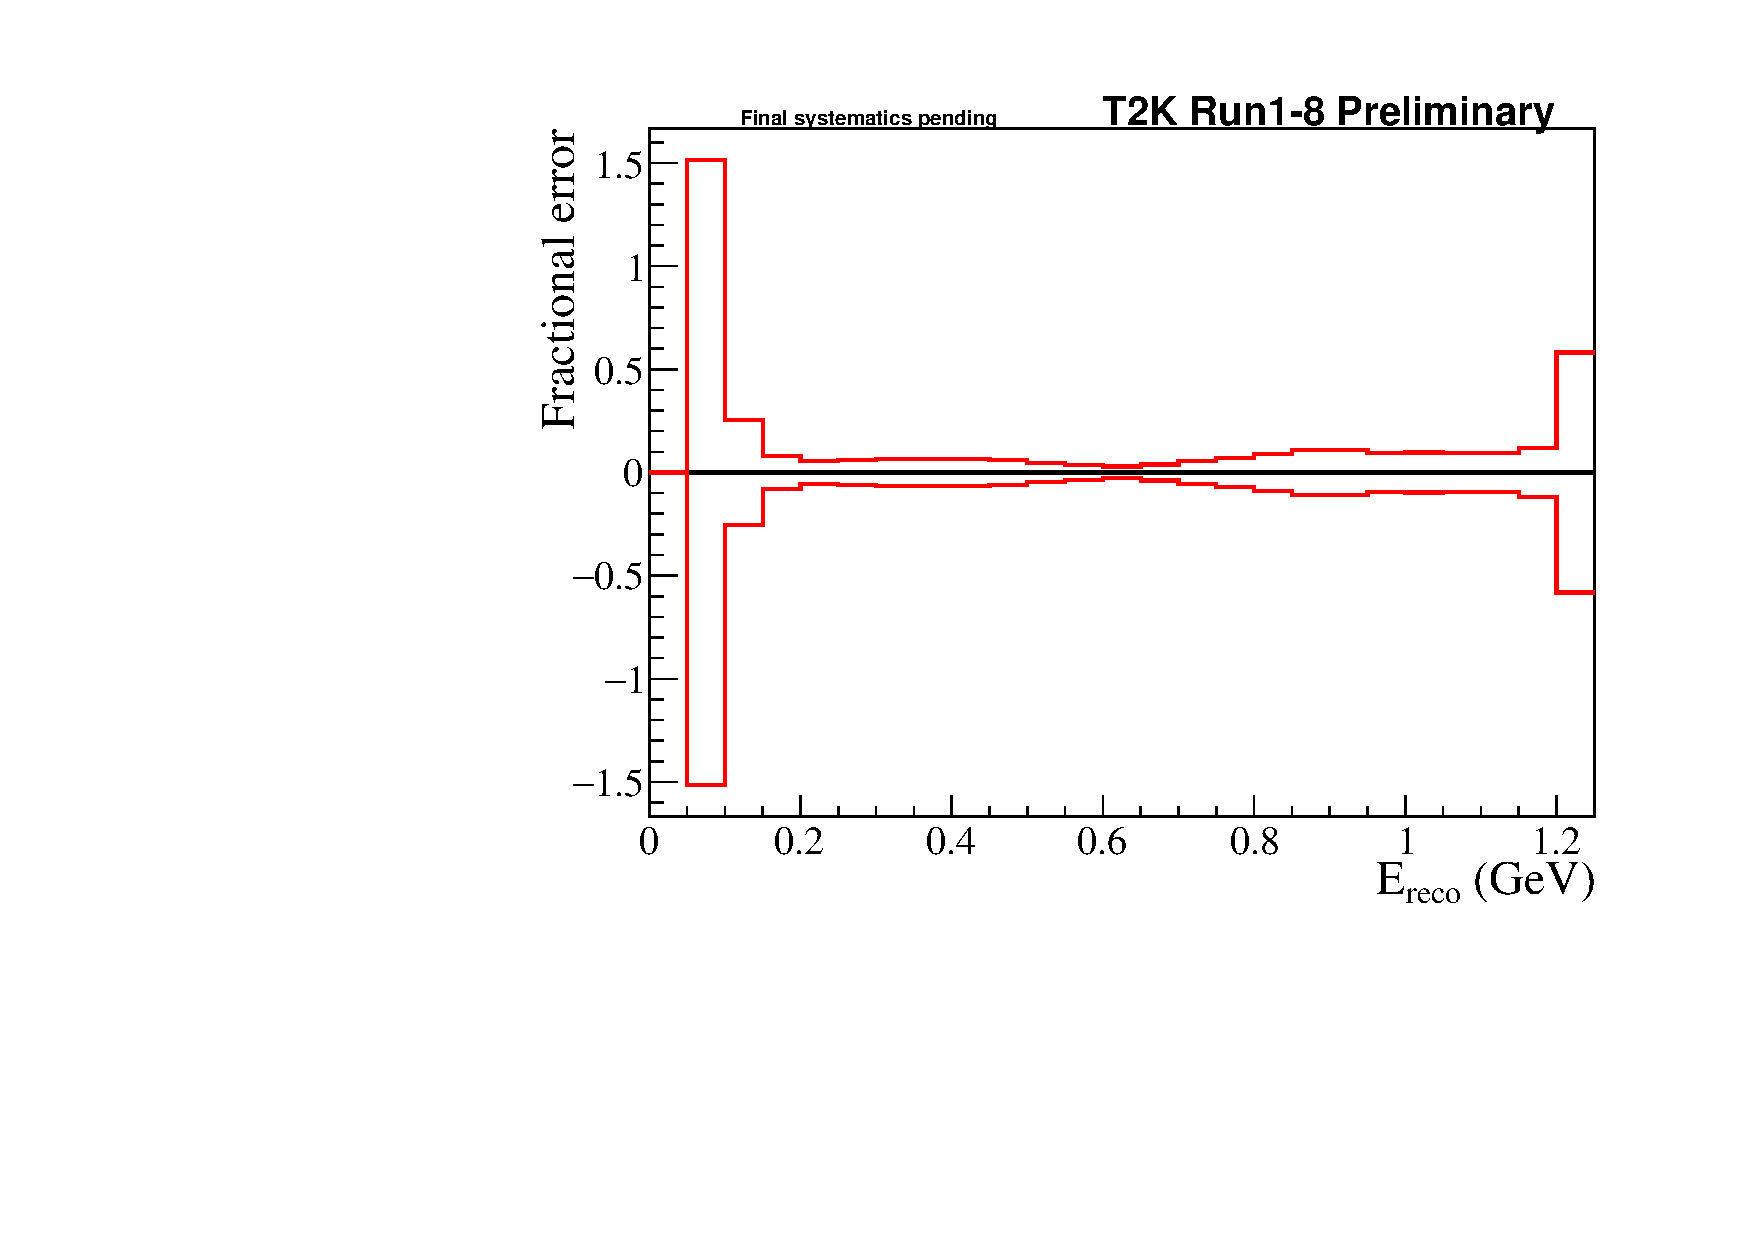
\includegraphics[width=0.9\textwidth]{systematics/envelopes/sk_errors/sk_error_table_1Re_skdet_envelope_fractional}
		\caption{Electron-like, neutrino mode}
	\end{subfigure}
	\begin{subfigure}[b]{0.49\textwidth}
		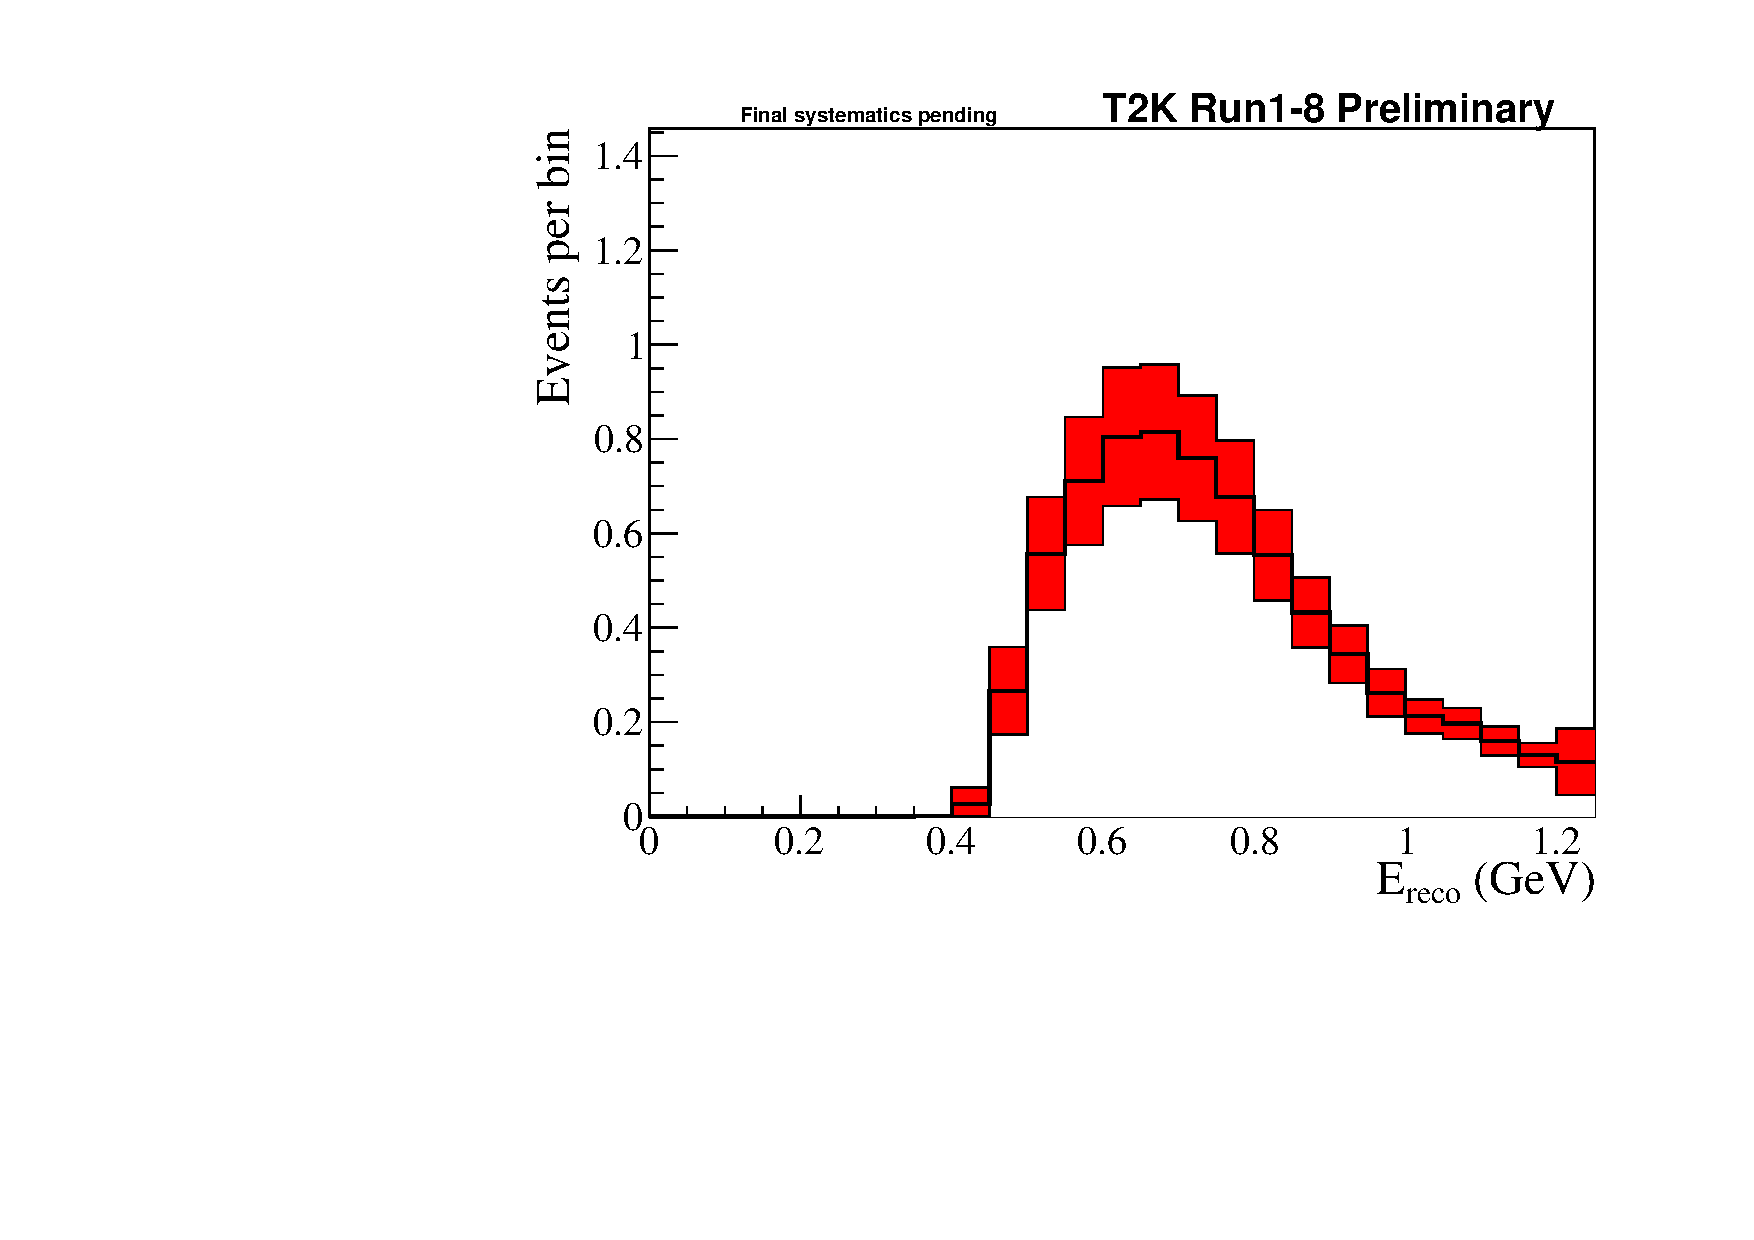
\includegraphics[width=0.9\textwidth]{systematics/envelopes/sk_errors/sk_error_table_MultiRe_skdet_envelope}
		\caption{\nueCConepi-like, neutrino mode}
	\end{subfigure}
	\begin{subfigure}[b]{0.49\textwidth}
		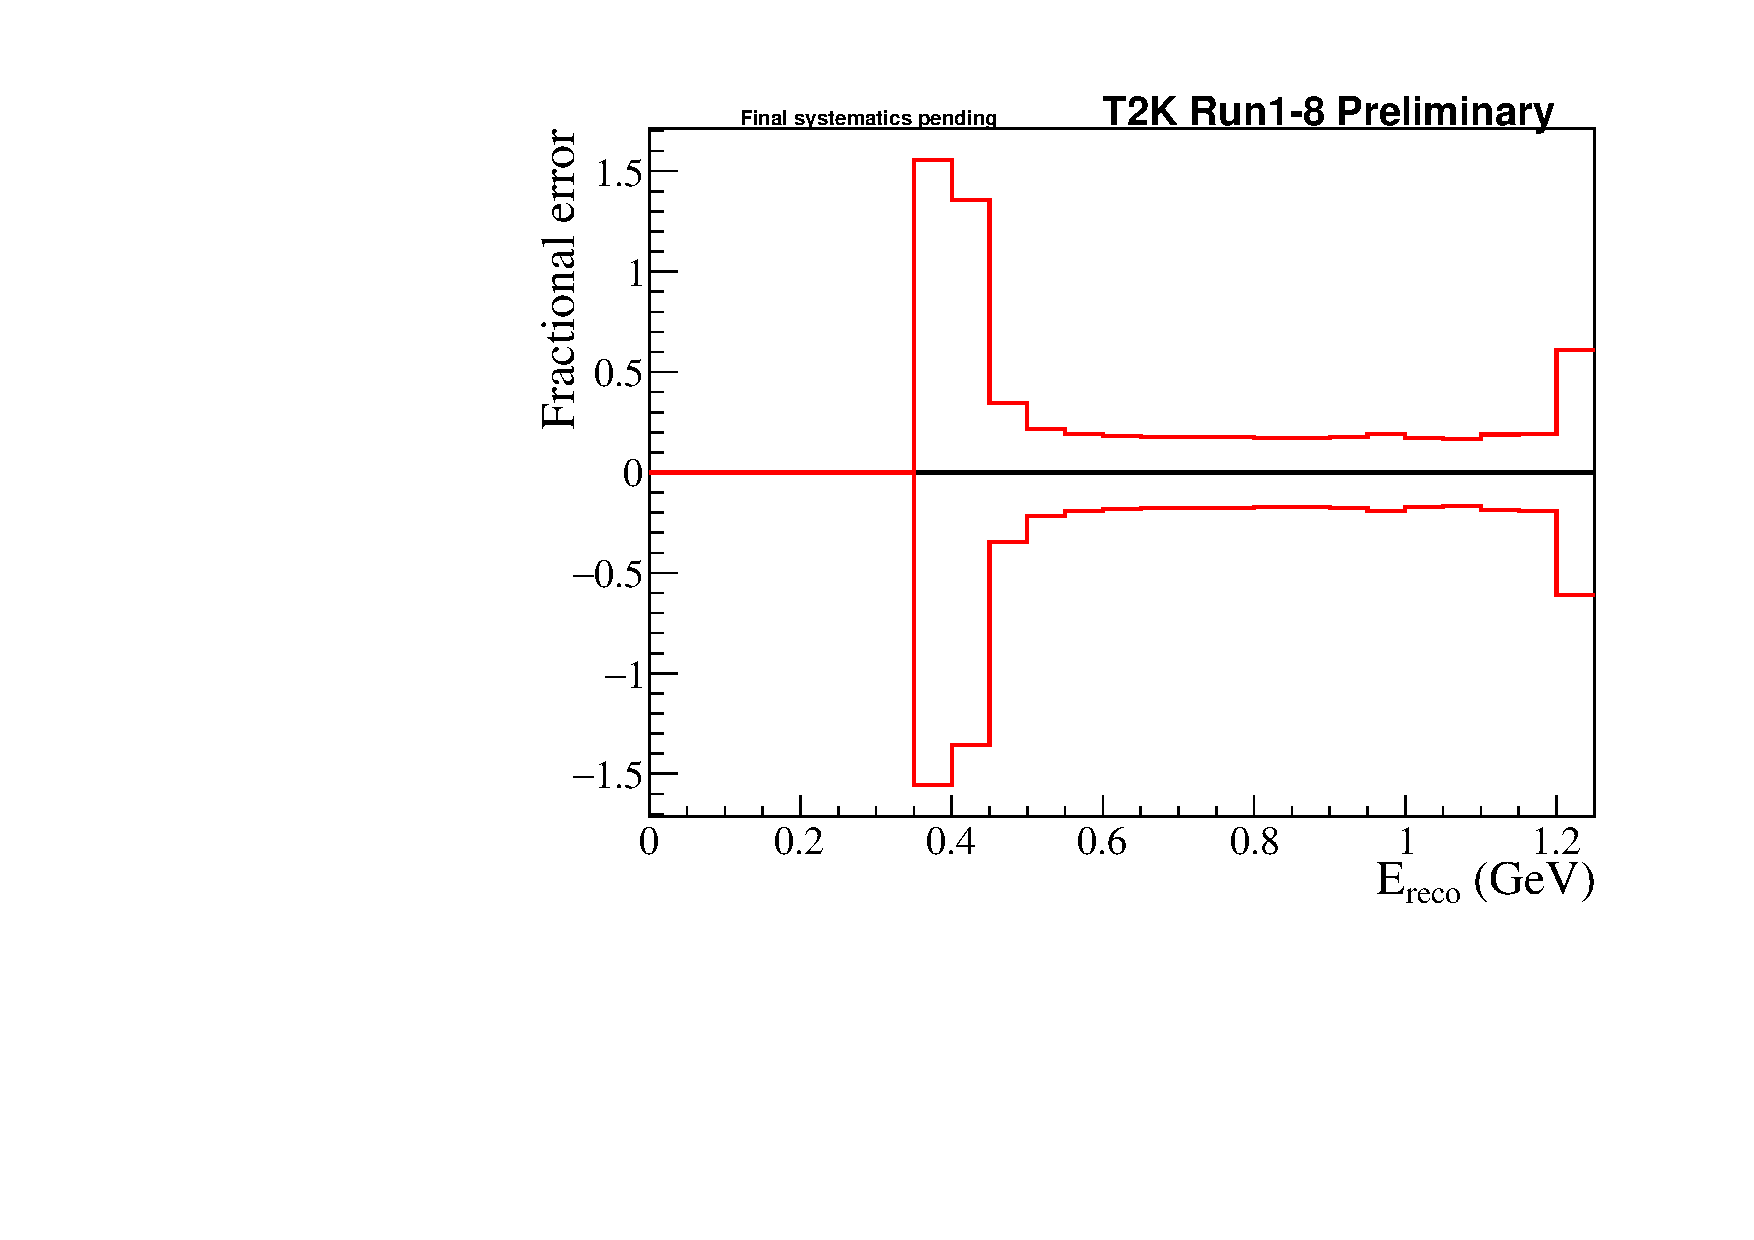
\includegraphics[width=0.9\textwidth]{systematics/envelopes/sk_errors/sk_error_table_MultiRe_skdet_envelope_fractional}
		\caption{\nueCConepi-like, neutrino mode}
	\end{subfigure}
	\caption {
		Error envelopes (left) and fractional error (right) for the reconstructed neutrino energy spectrum for Super-K detector systematic parameters. \num{1e4} toys are generated for the Asimov data set A with randomized systematic parameters with correlations taken into account.
	}
	\label{fig:sk_envelopes_skdet}
\end{figure*}
\clearpage

\begin{figure*}
	\center
	\begin{subfigure}[b]{0.49\textwidth}
		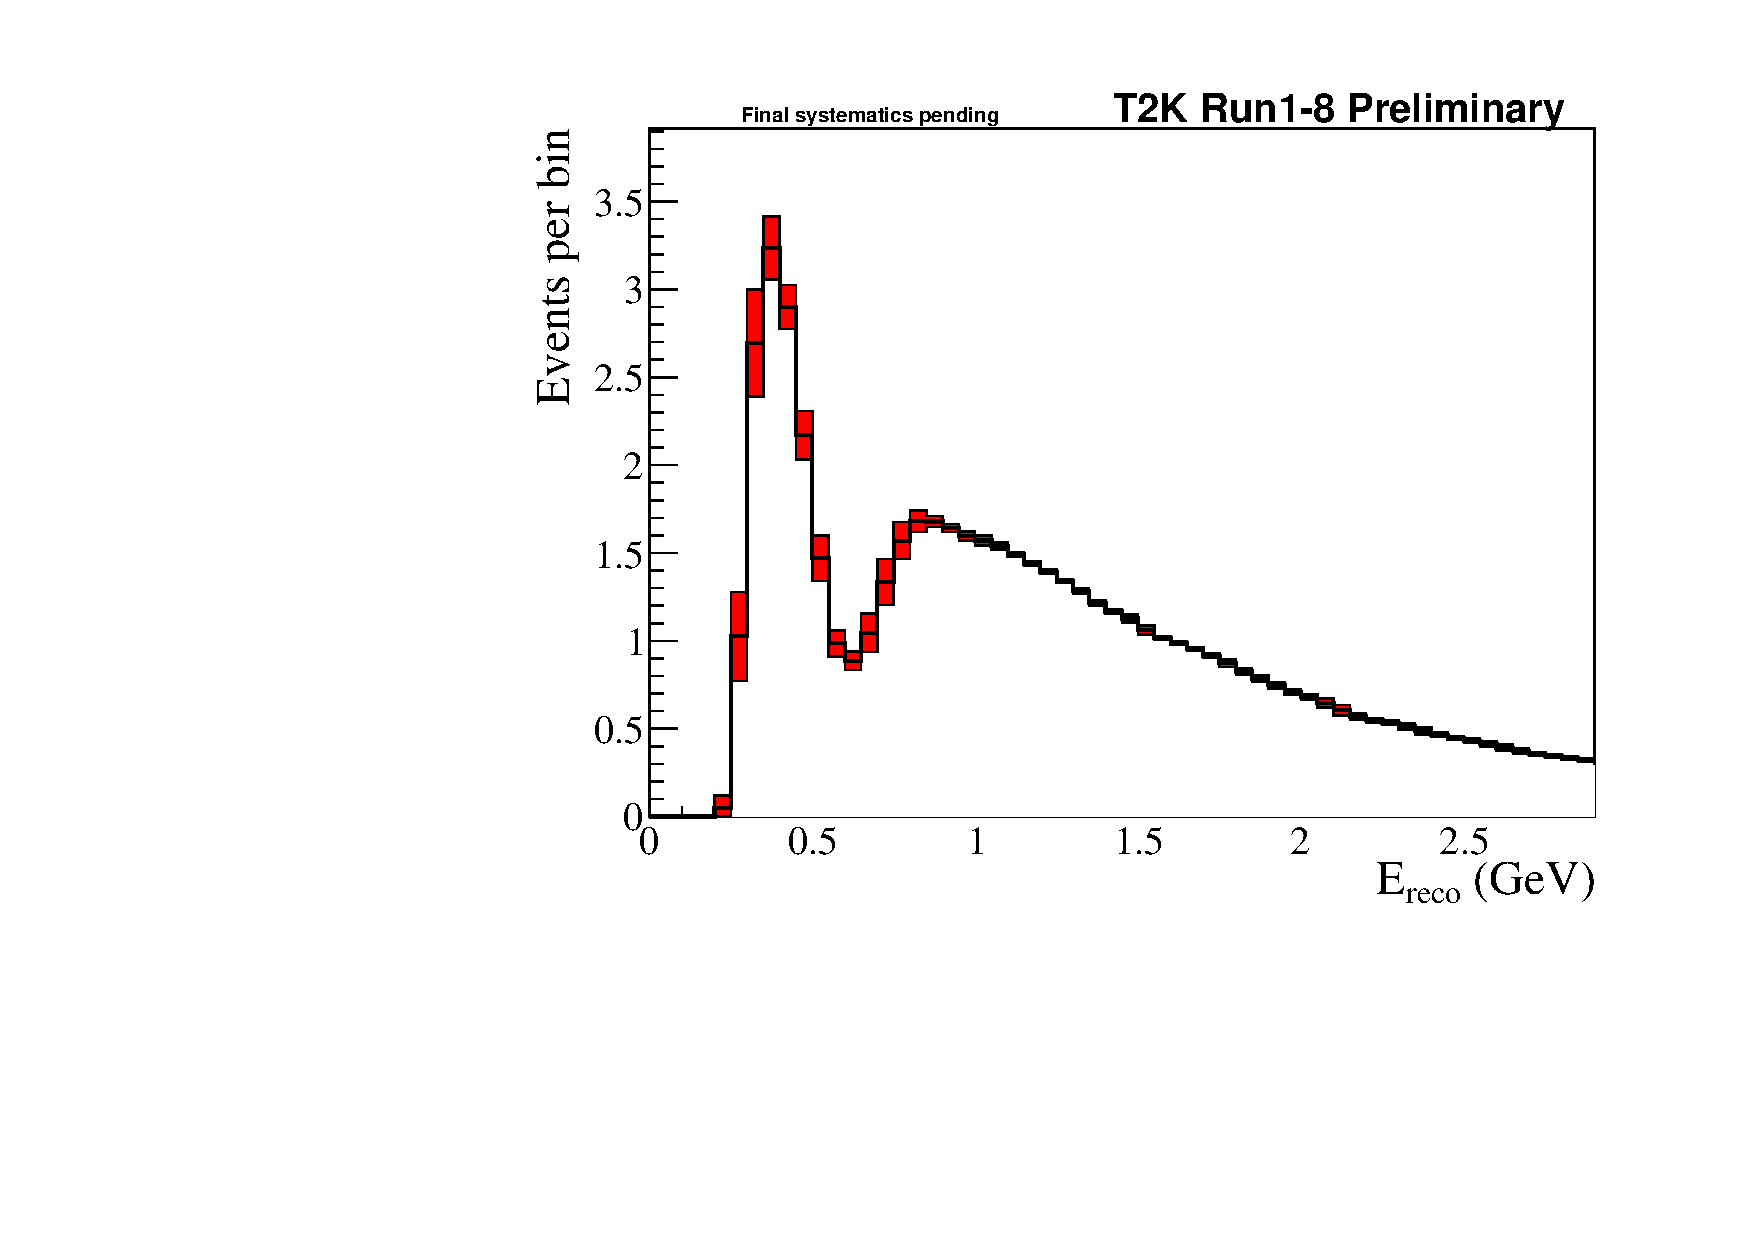
\includegraphics[width=0.9\textwidth]{systematics/envelopes/sk_errors/sk_error_table_RHC1Rmu_skdet_envelope}
		\caption{Muon-like, antineutrino mode}
	\end{subfigure}
	\begin{subfigure}[b]{0.49\textwidth}
		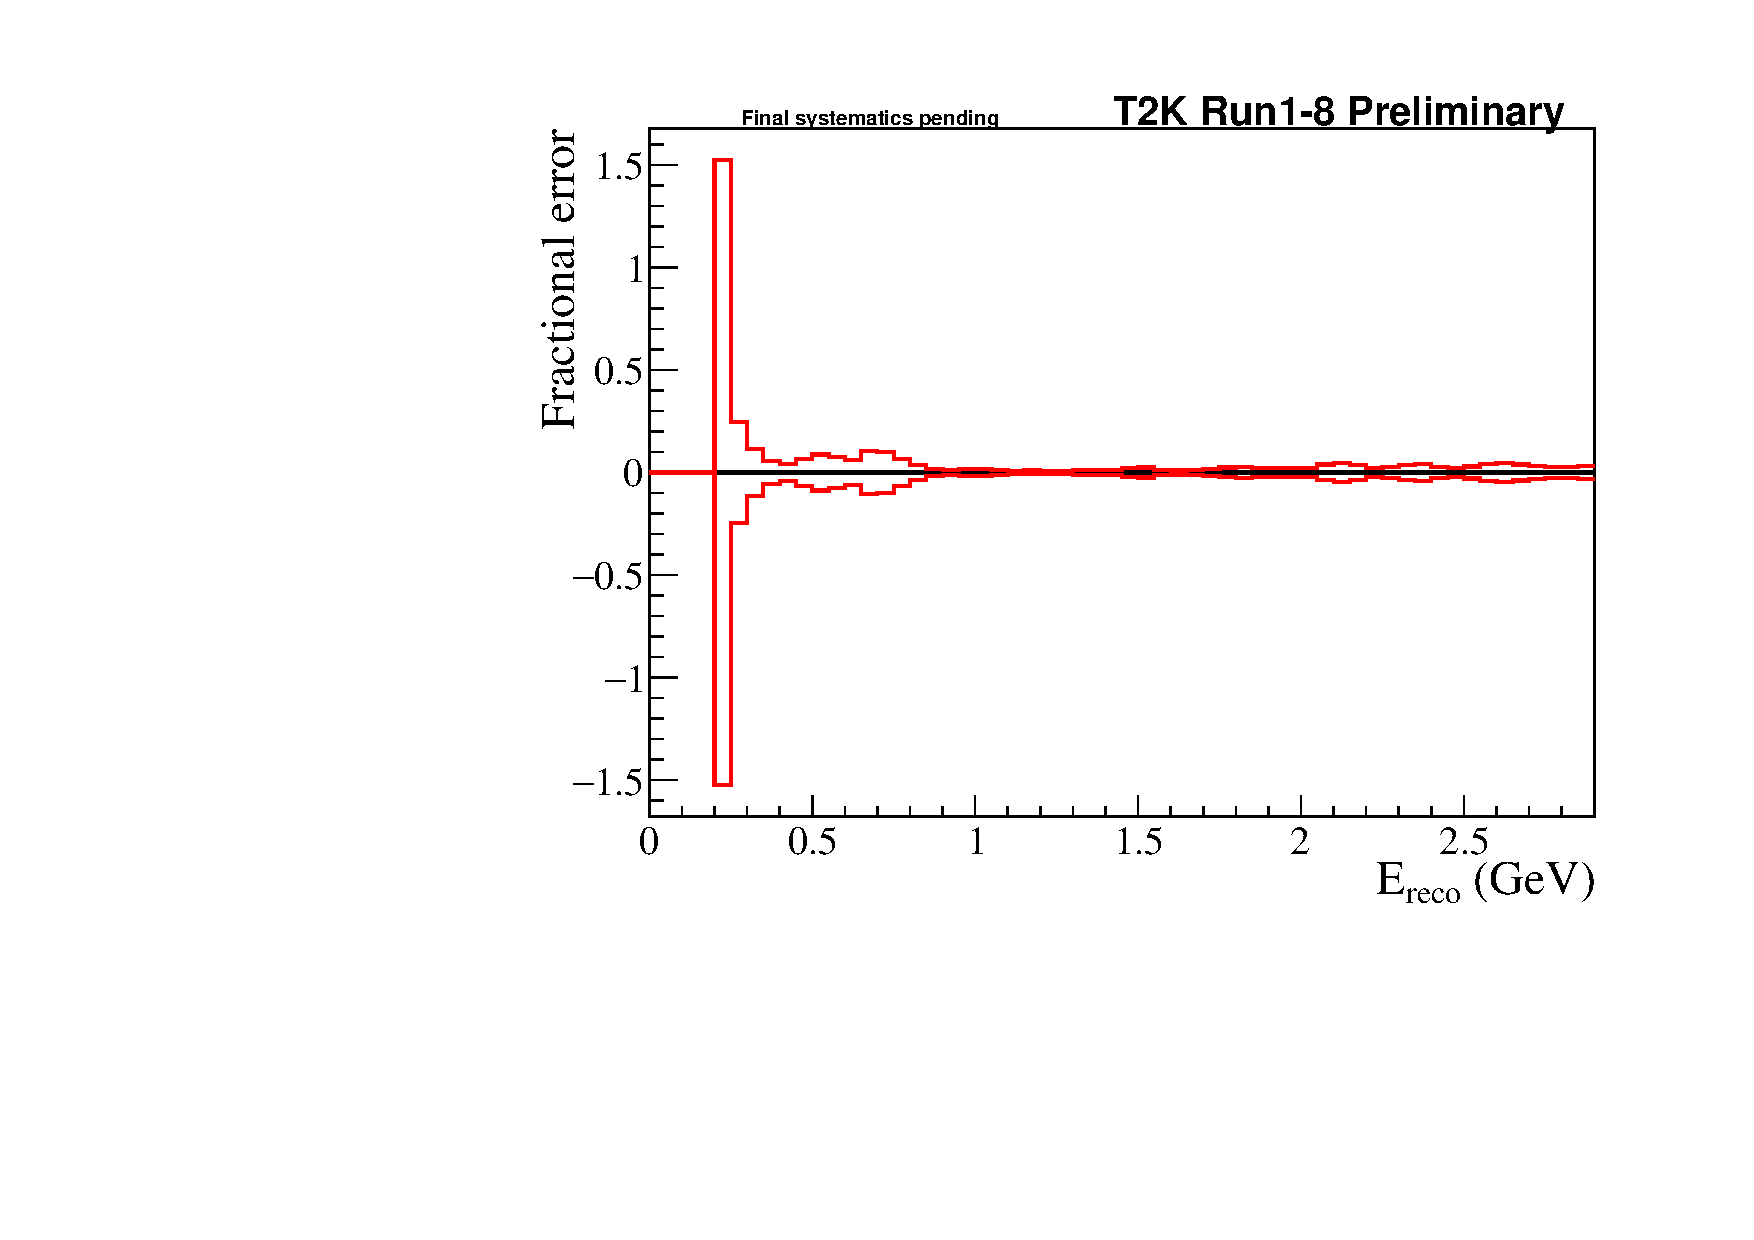
\includegraphics[width=0.9\textwidth]{systematics/envelopes/sk_errors/sk_error_table_RHC1Rmu_skdet_envelope_fractional}
		\caption{Muon-like, antineutrino mode}
	\end{subfigure}
	\begin{subfigure}[b]{0.49\textwidth}
		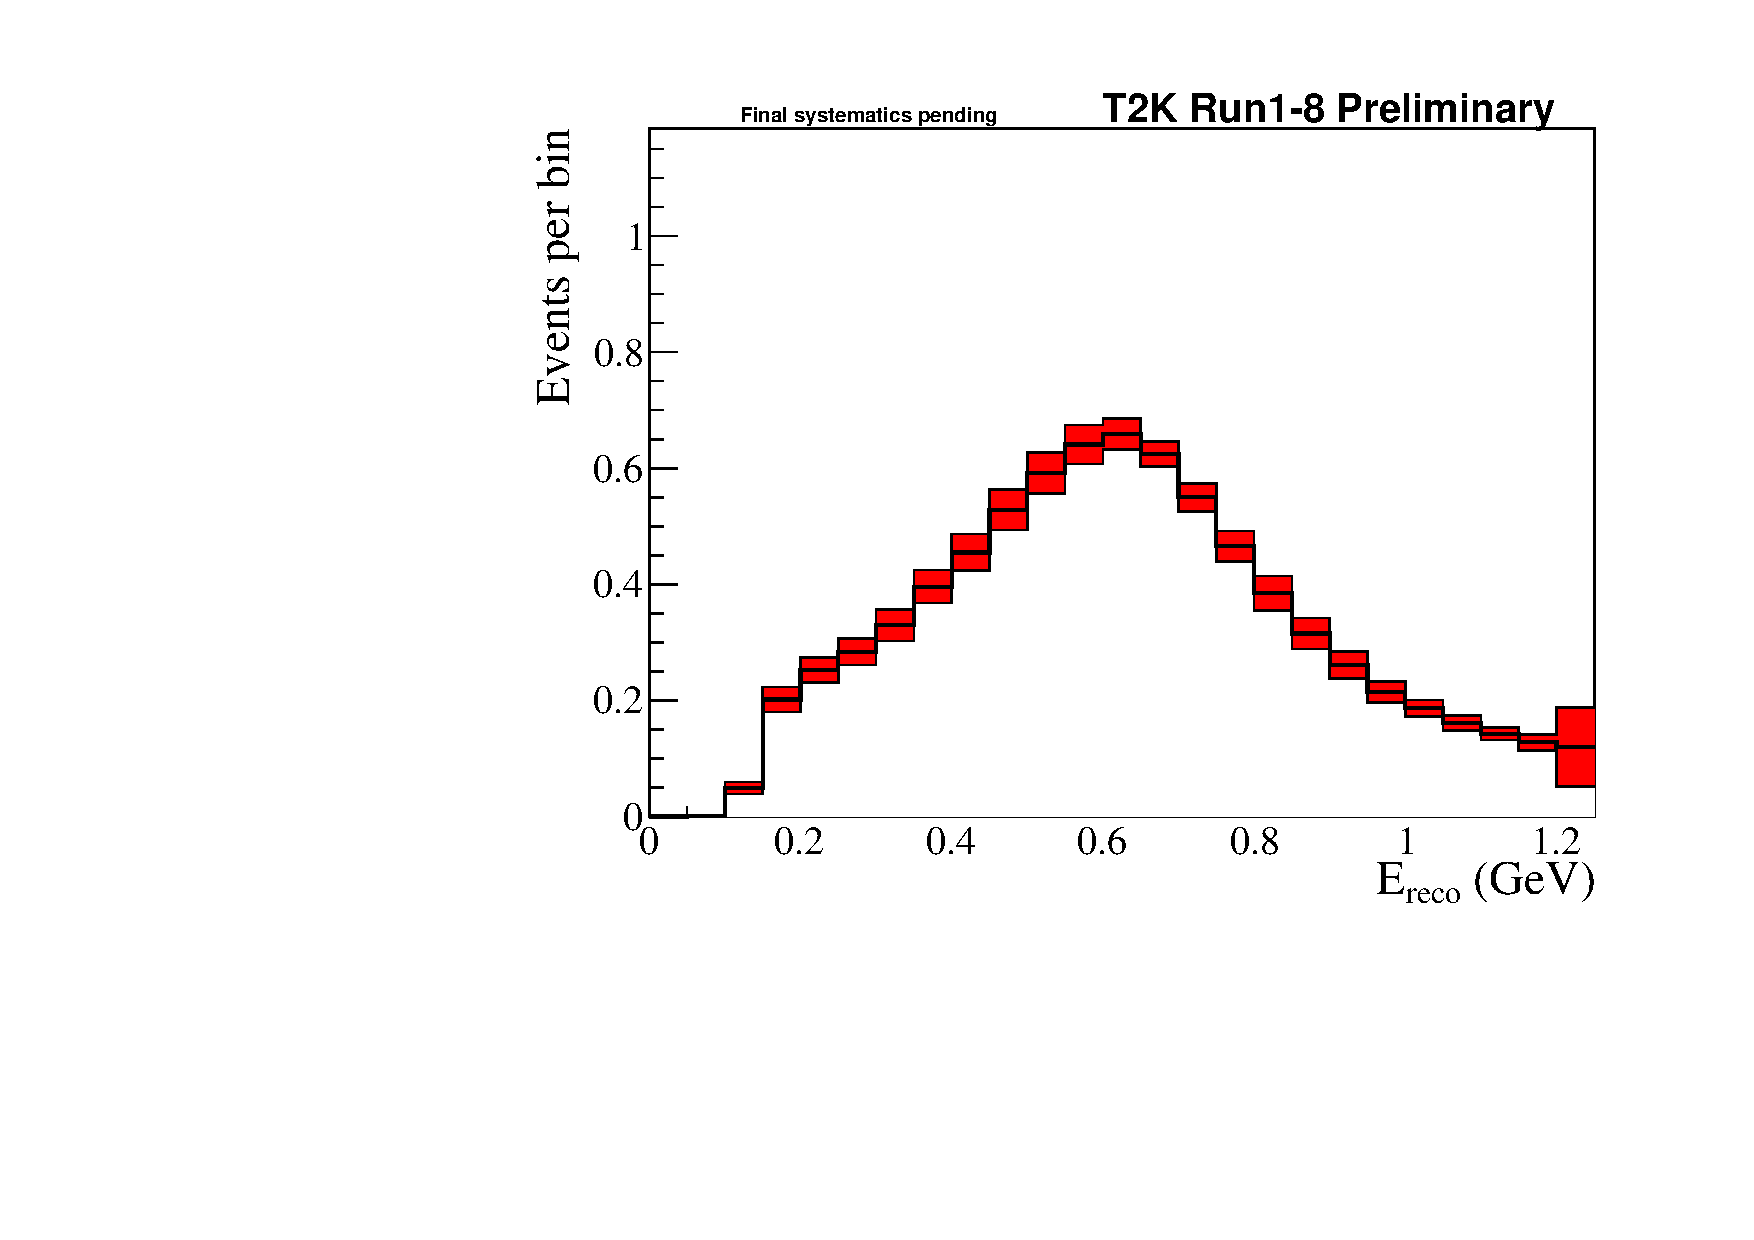
\includegraphics[width=0.9\textwidth]{systematics/envelopes/sk_errors/sk_error_table_RHC1Re_skdet_envelope}
		\caption{Electron-like antineutrino mode}
	\end{subfigure}
	\begin{subfigure}[b]{0.49\textwidth}
		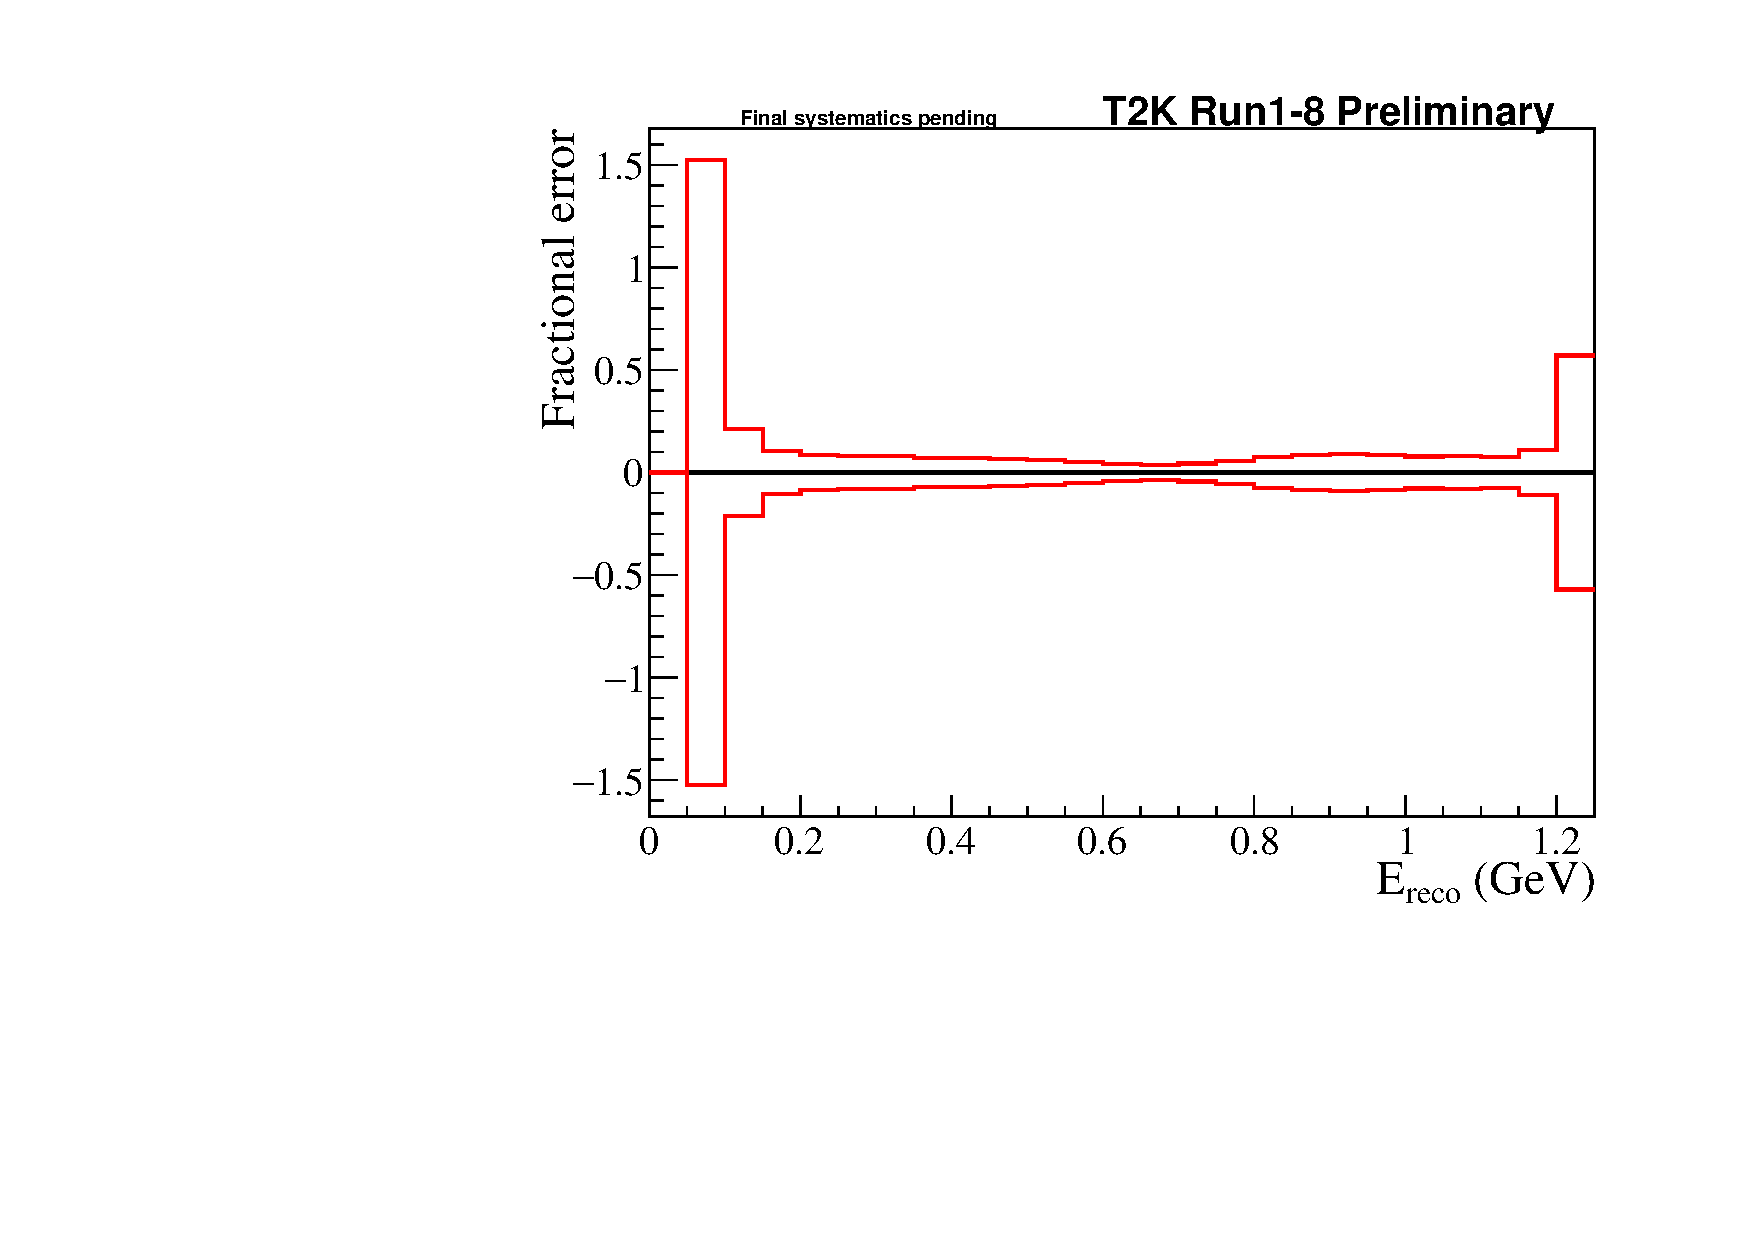
\includegraphics[width=0.9\textwidth]{systematics/envelopes/sk_errors/sk_error_table_RHC1Re_skdet_envelope_fractional}
		\caption{Electron-like antineutrino mode}
	\end{subfigure}
	\caption {
		Error envelopes (left) and fractional error (right) for the reconstructed neutrino energy spectrum for Super-K detector systematic parameters. \num{1e4} toys are generated for the Asimov data set A with randomized systematic parameters with correlations taken into account.
	}
	\label{fig:sk_envelopes_skdet_b}
\end{figure*}
\clearpage
\begin{figure*}
	\center
	\begin{subfigure}[b]{0.49\textwidth}
		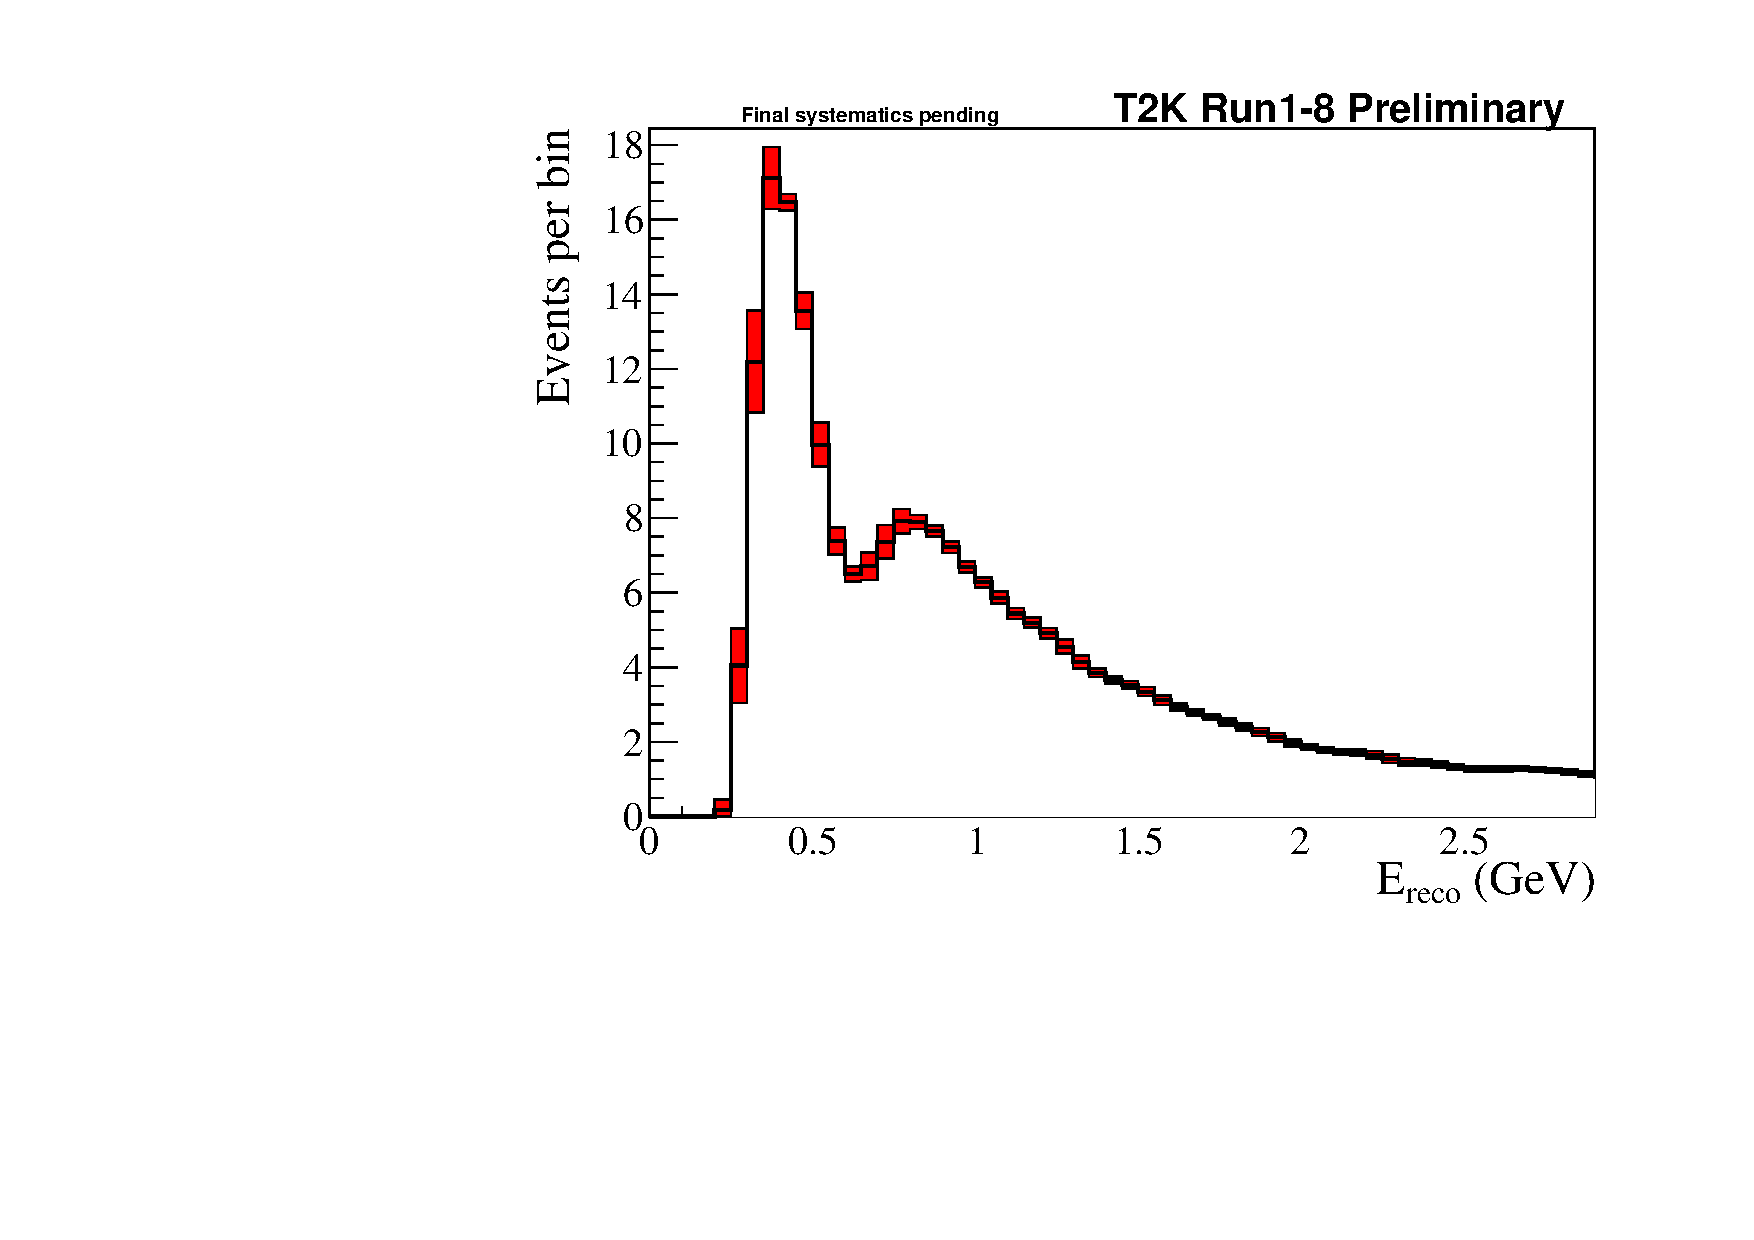
\includegraphics[width=0.9\textwidth]{systematics/envelopes/sk_errors/sk_error_table_1Rmu_skfsi_envelope}
		\caption{Muon-like, neutrino mode}
	\end{subfigure}
	\begin{subfigure}[b]{0.49\textwidth}
		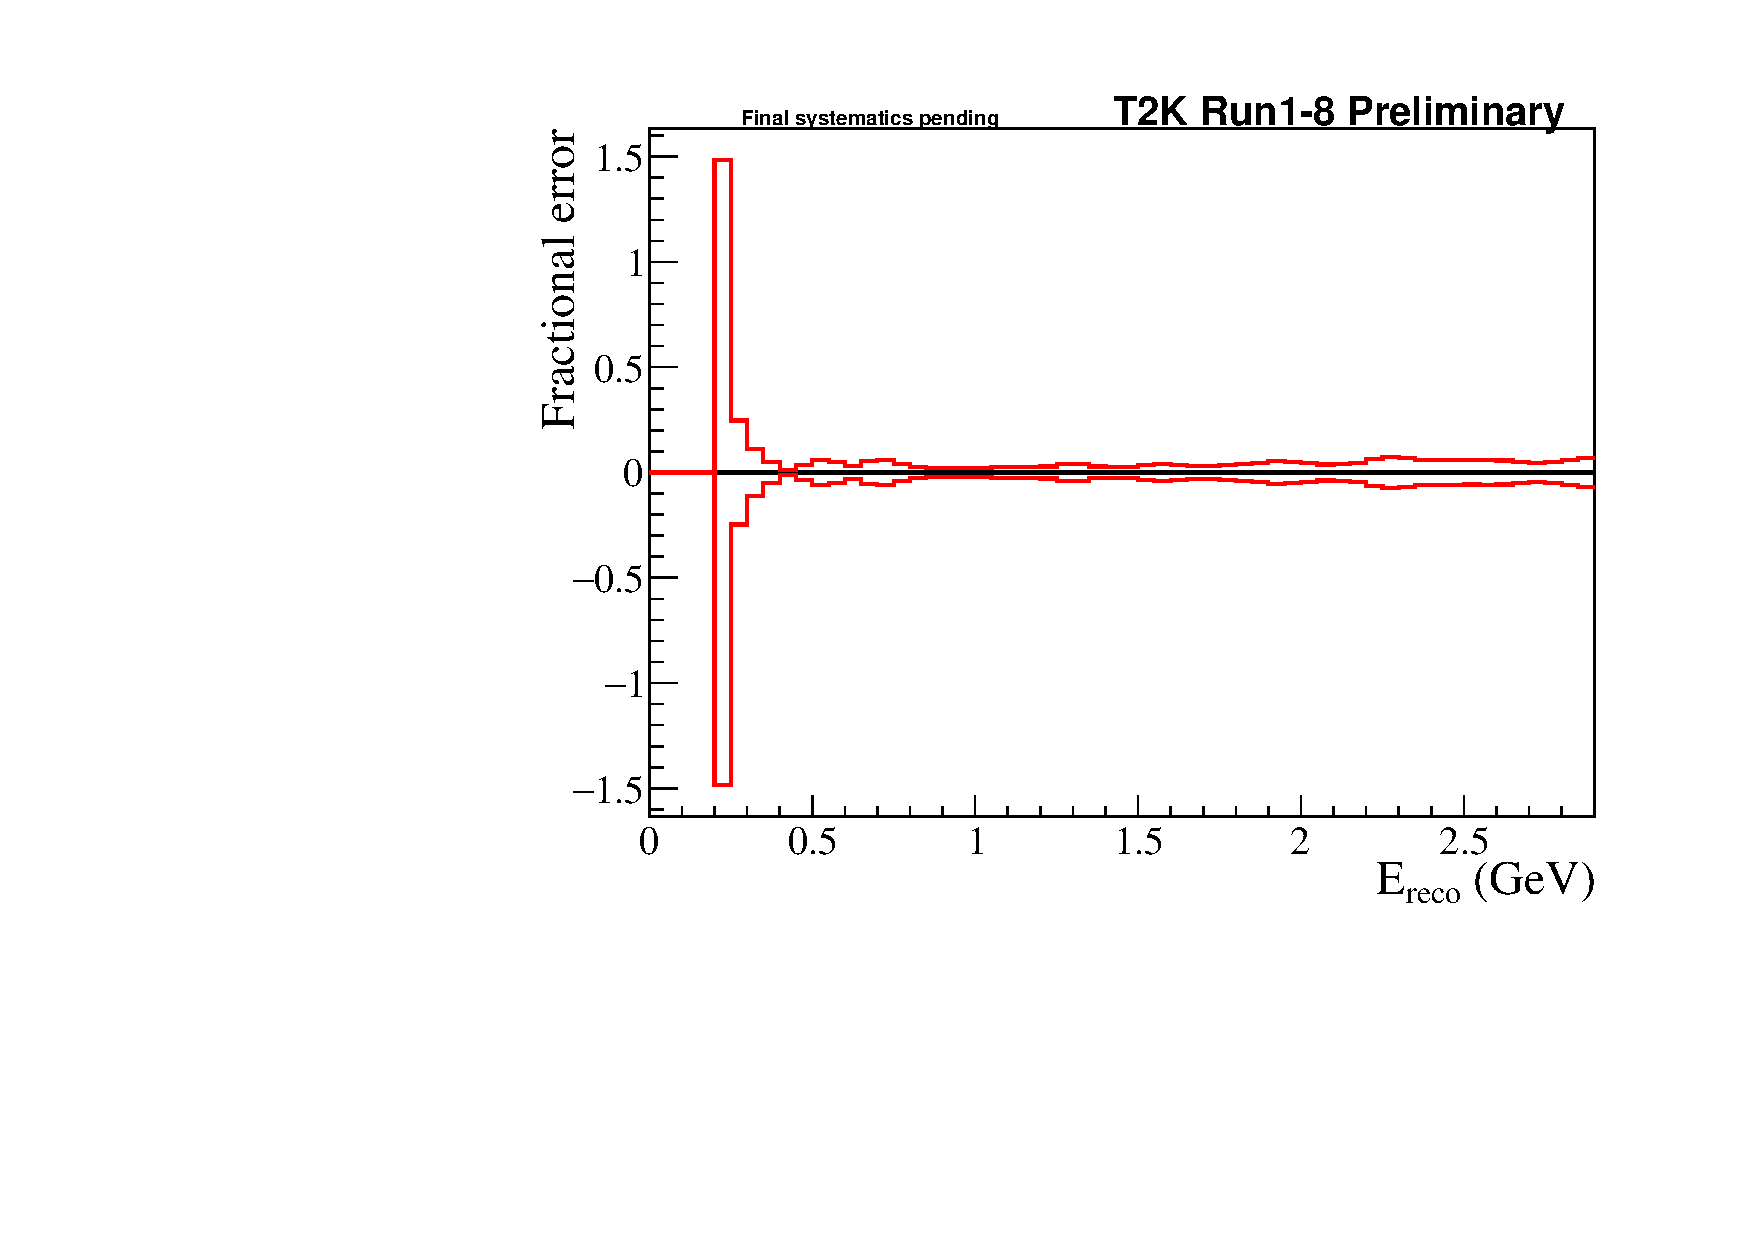
\includegraphics[width=0.9\textwidth]{systematics/envelopes/sk_errors/sk_error_table_1Rmu_skfsi_envelope_fractional}
		\caption{Muon-like, neutrino mode}
	\end{subfigure}
	\begin{subfigure}[b]{0.49\textwidth}
		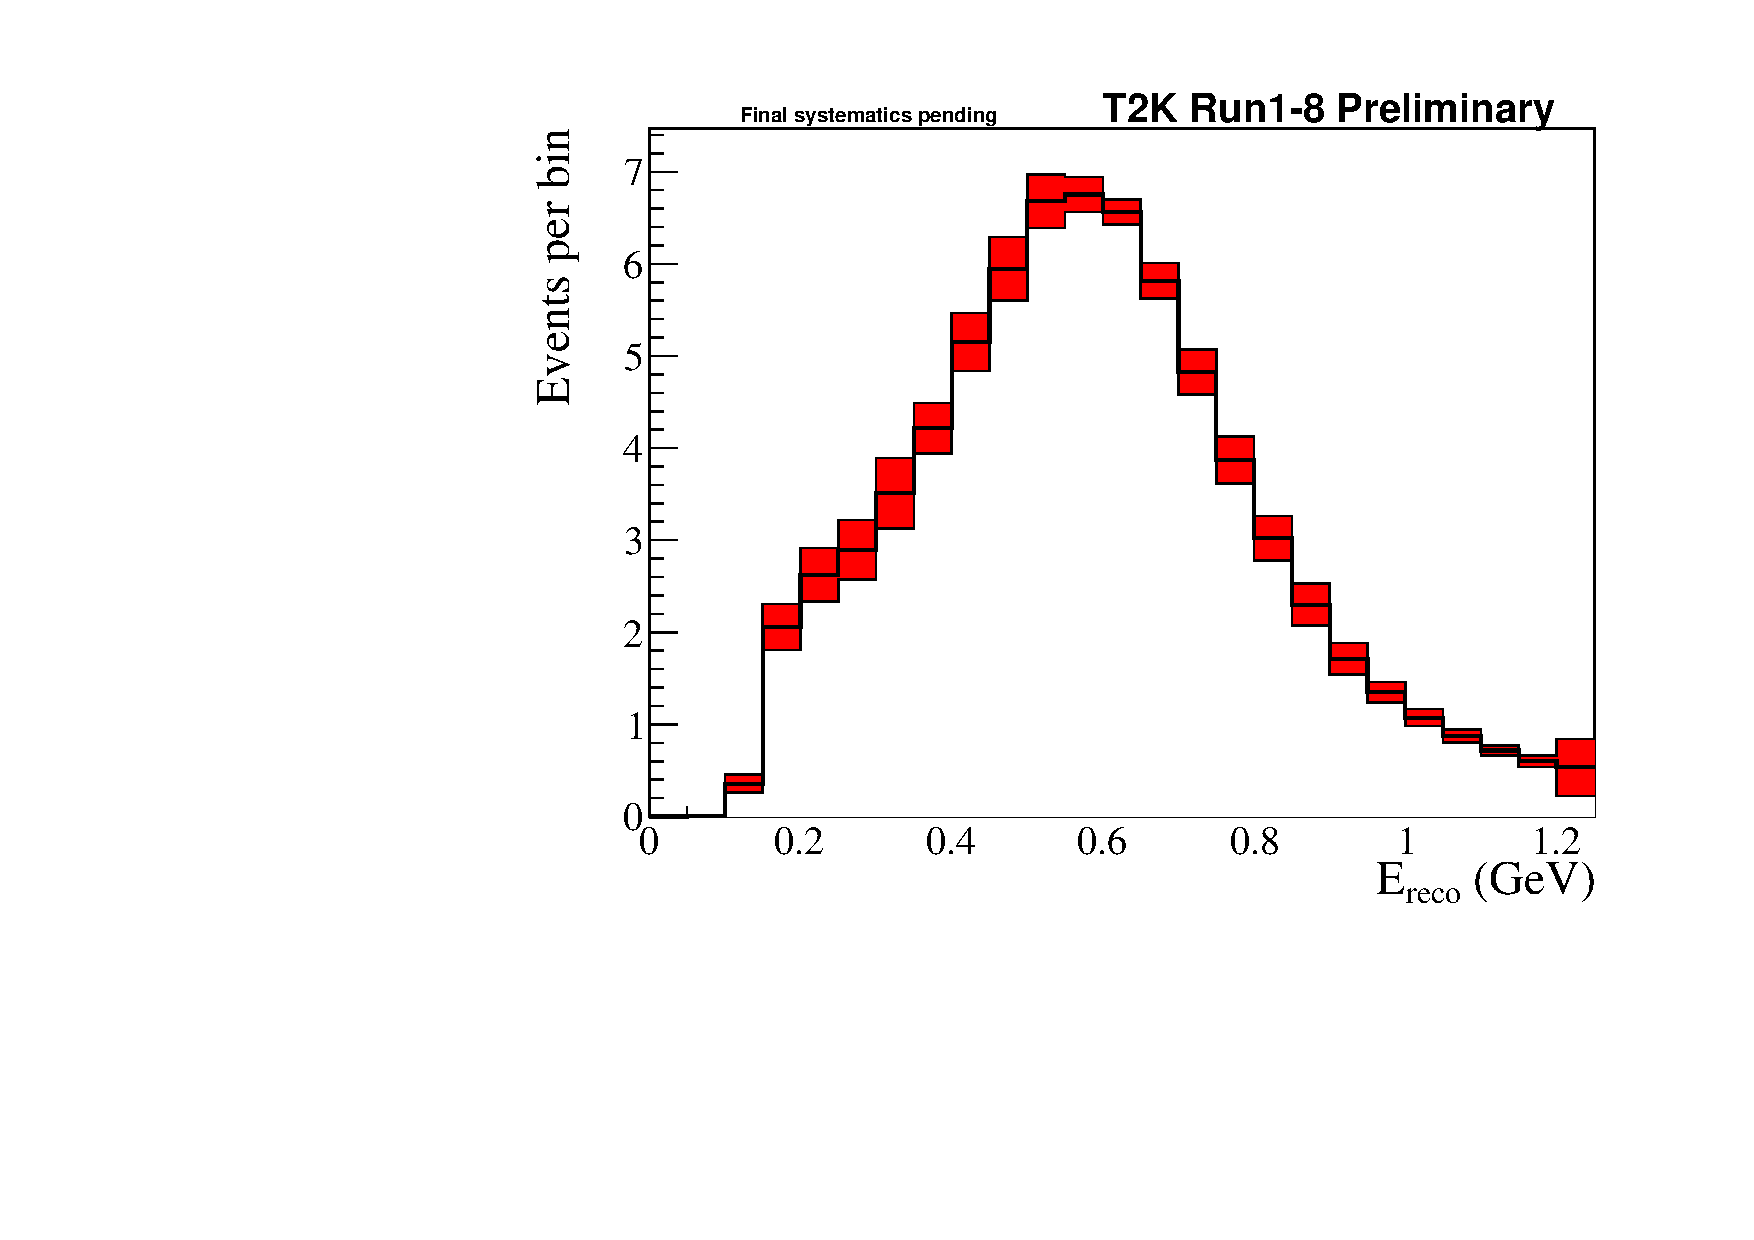
\includegraphics[width=0.9\textwidth]{systematics/envelopes/sk_errors/sk_error_table_1Re_skfsi_envelope}
		\caption{Electron-like, neutrino mode}
	\end{subfigure}
	\begin{subfigure}[b]{0.49\textwidth}
		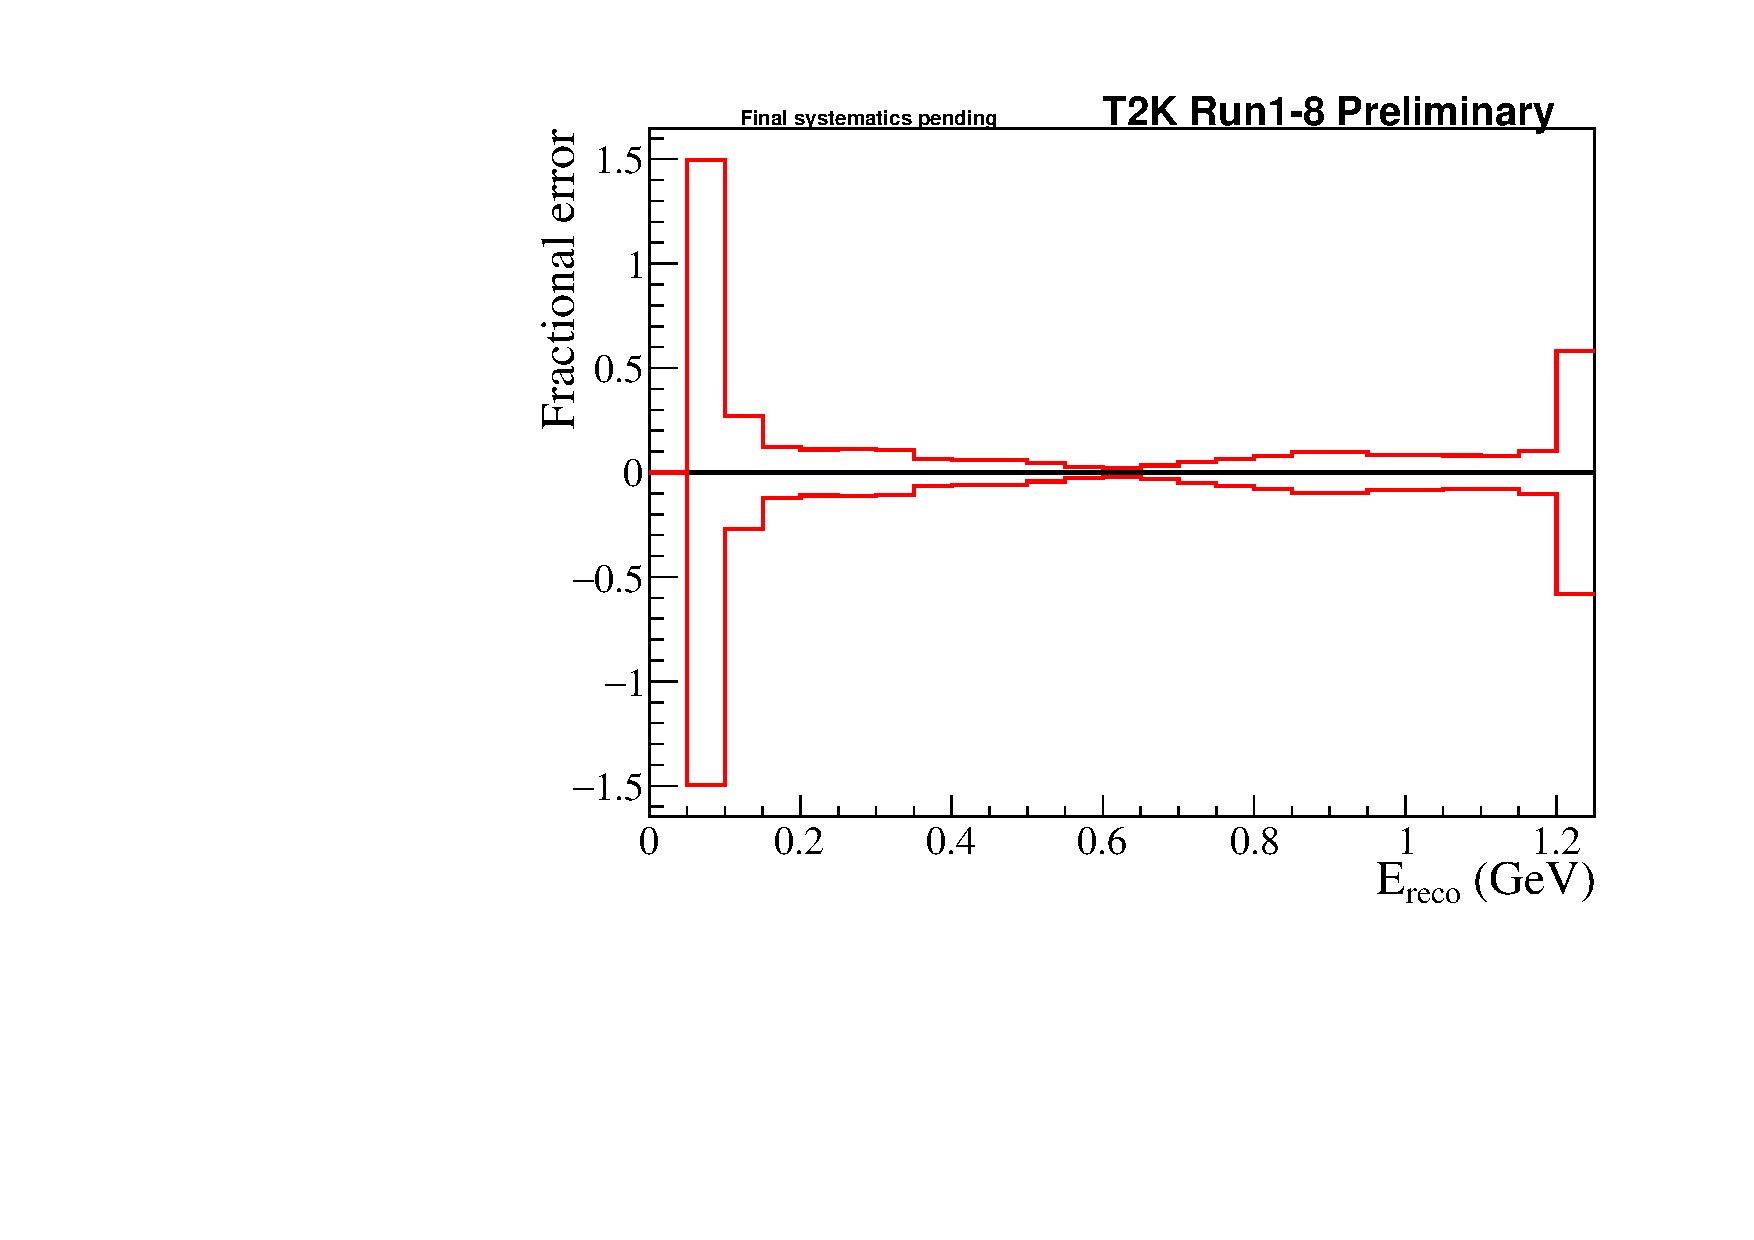
\includegraphics[width=0.9\textwidth]{systematics/envelopes/sk_errors/sk_error_table_1Re_skfsi_envelope_fractional}
		\caption{Electron-like, neutrino mode}
	\end{subfigure}
	\begin{subfigure}[b]{0.49\textwidth}
		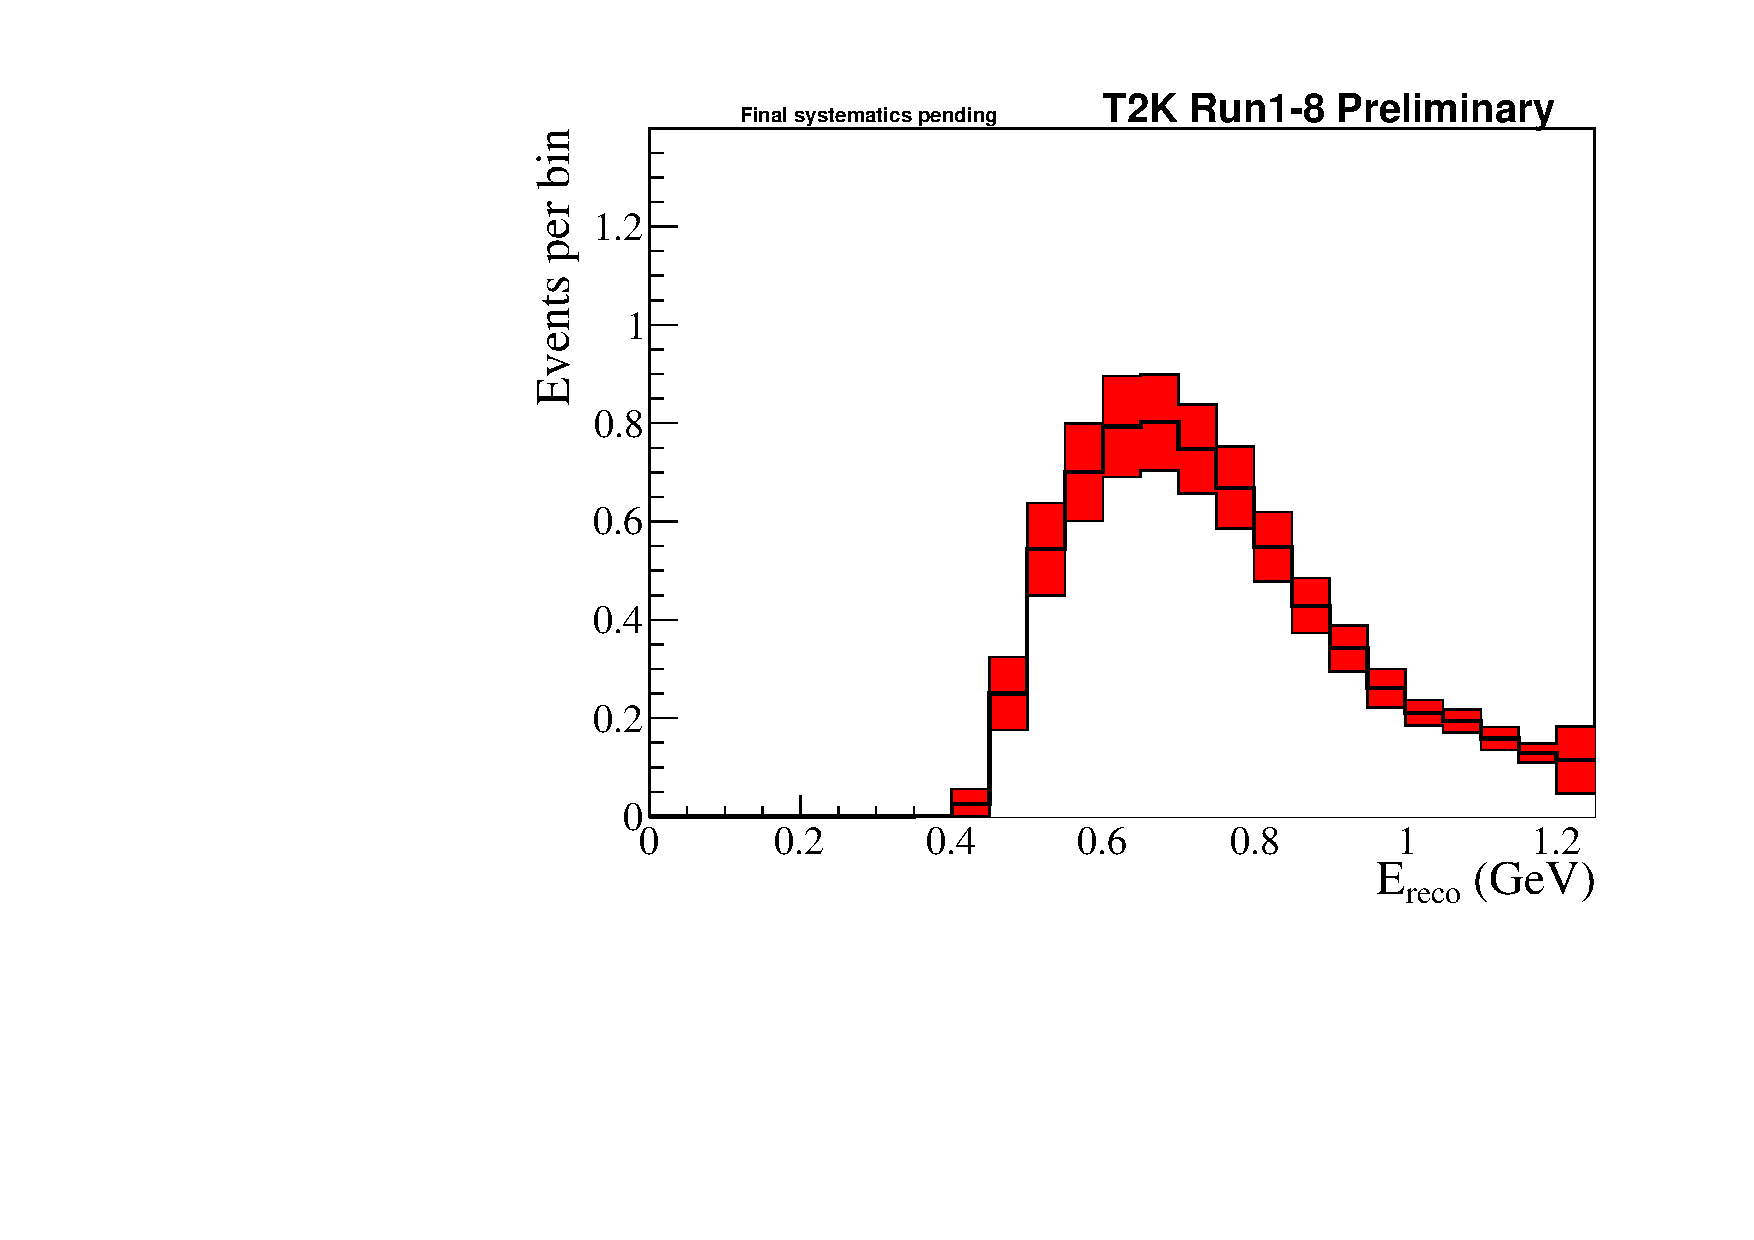
\includegraphics[width=0.9\textwidth]{systematics/envelopes/sk_errors/sk_error_table_MultiRe_skfsi_envelope}
		\caption{\nueCConepi-like, neutrino mode}
	\end{subfigure}
	\begin{subfigure}[b]{0.49\textwidth}
		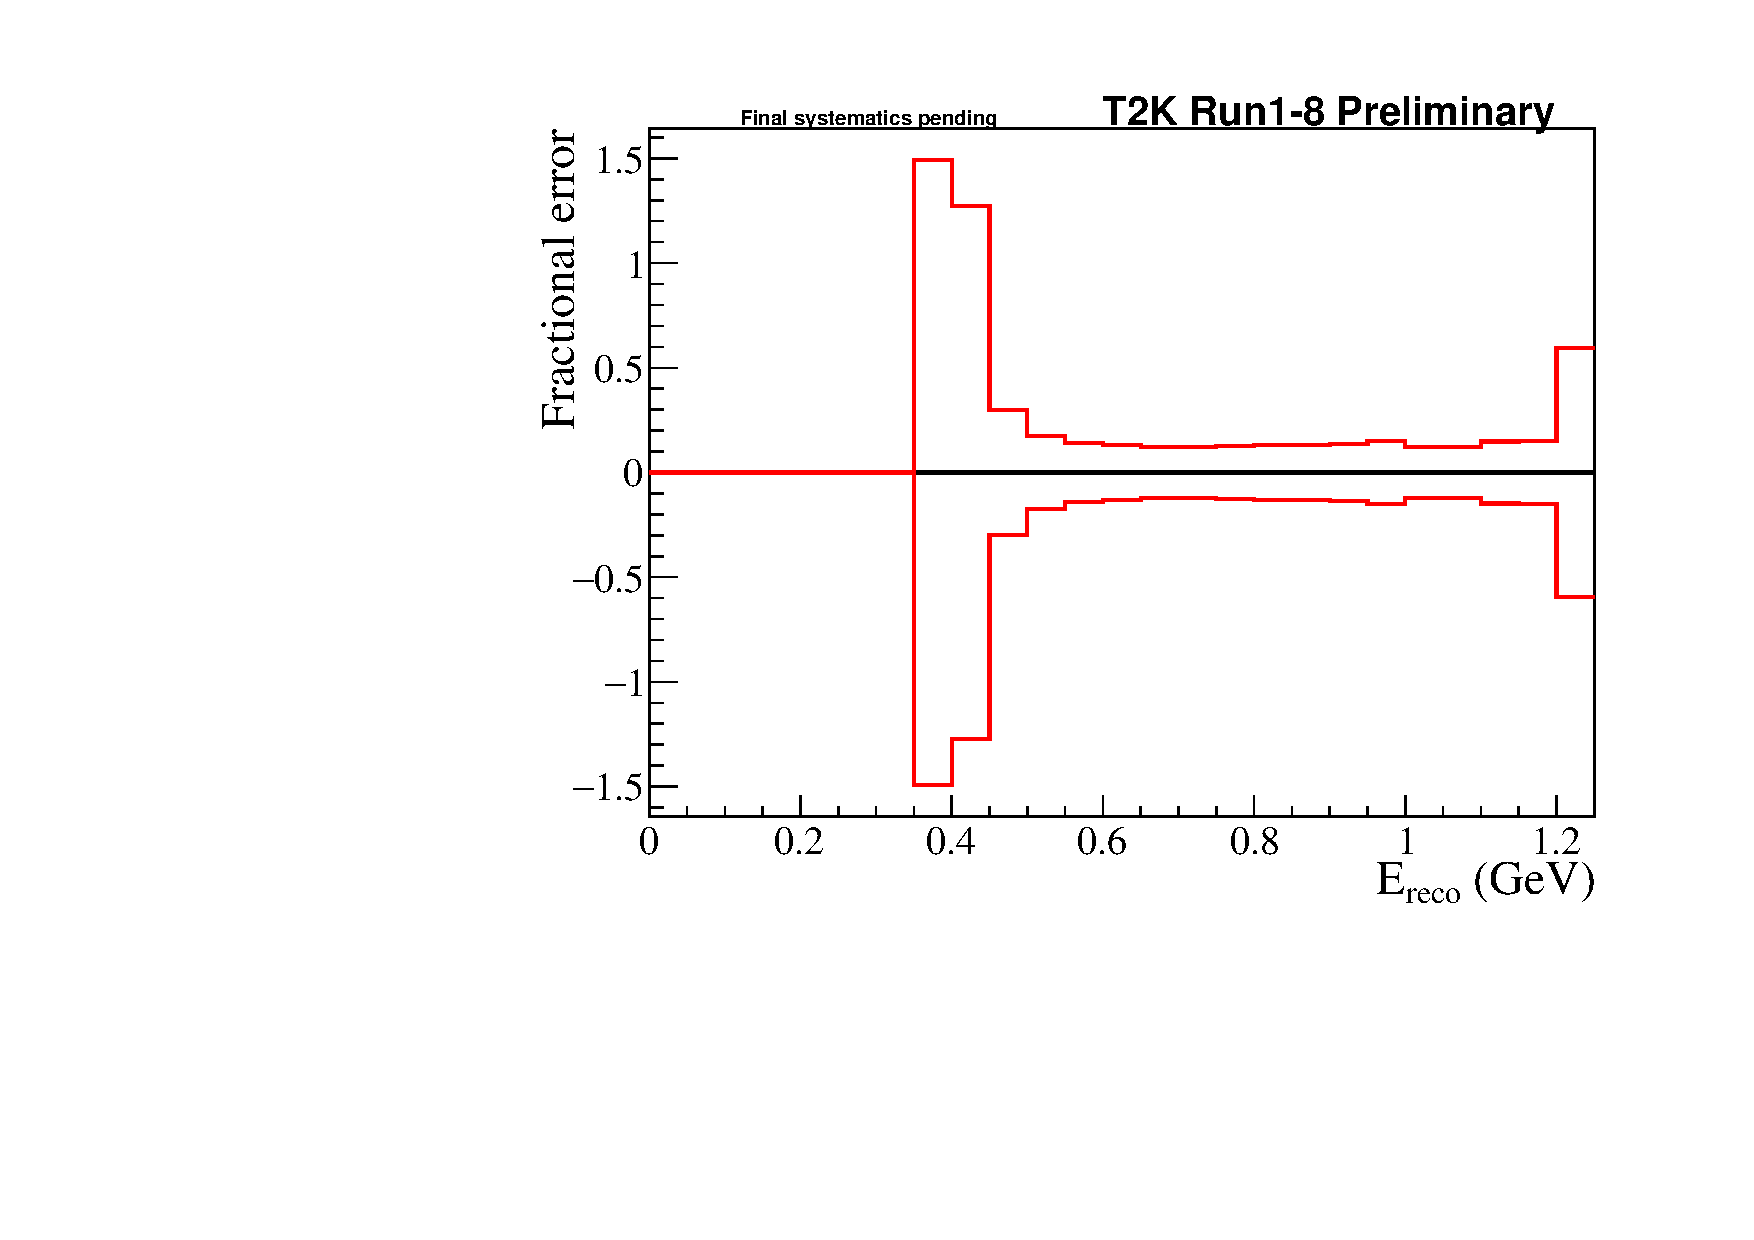
\includegraphics[width=0.9\textwidth]{systematics/envelopes/sk_errors/sk_error_table_MultiRe_skfsi_envelope_fractional}
		\caption{\nueCConepi-like, neutrino mode}
	\end{subfigure}
	\caption {
		Error envelopes (left) and fractional error (right) for the reconstructed neutrino energy spectrum for Super-K FSI+SI+PN systematic parameters. \num{1e4} toys are generated for the Asimov data set A with randomized systematic parameters with correlations taken into account.
	}
	\label{fig:sk_envelopes_skfsi}
\end{figure*}
\clearpage

\begin{figure*}
	\center
	\begin{subfigure}[b]{0.49\textwidth}
		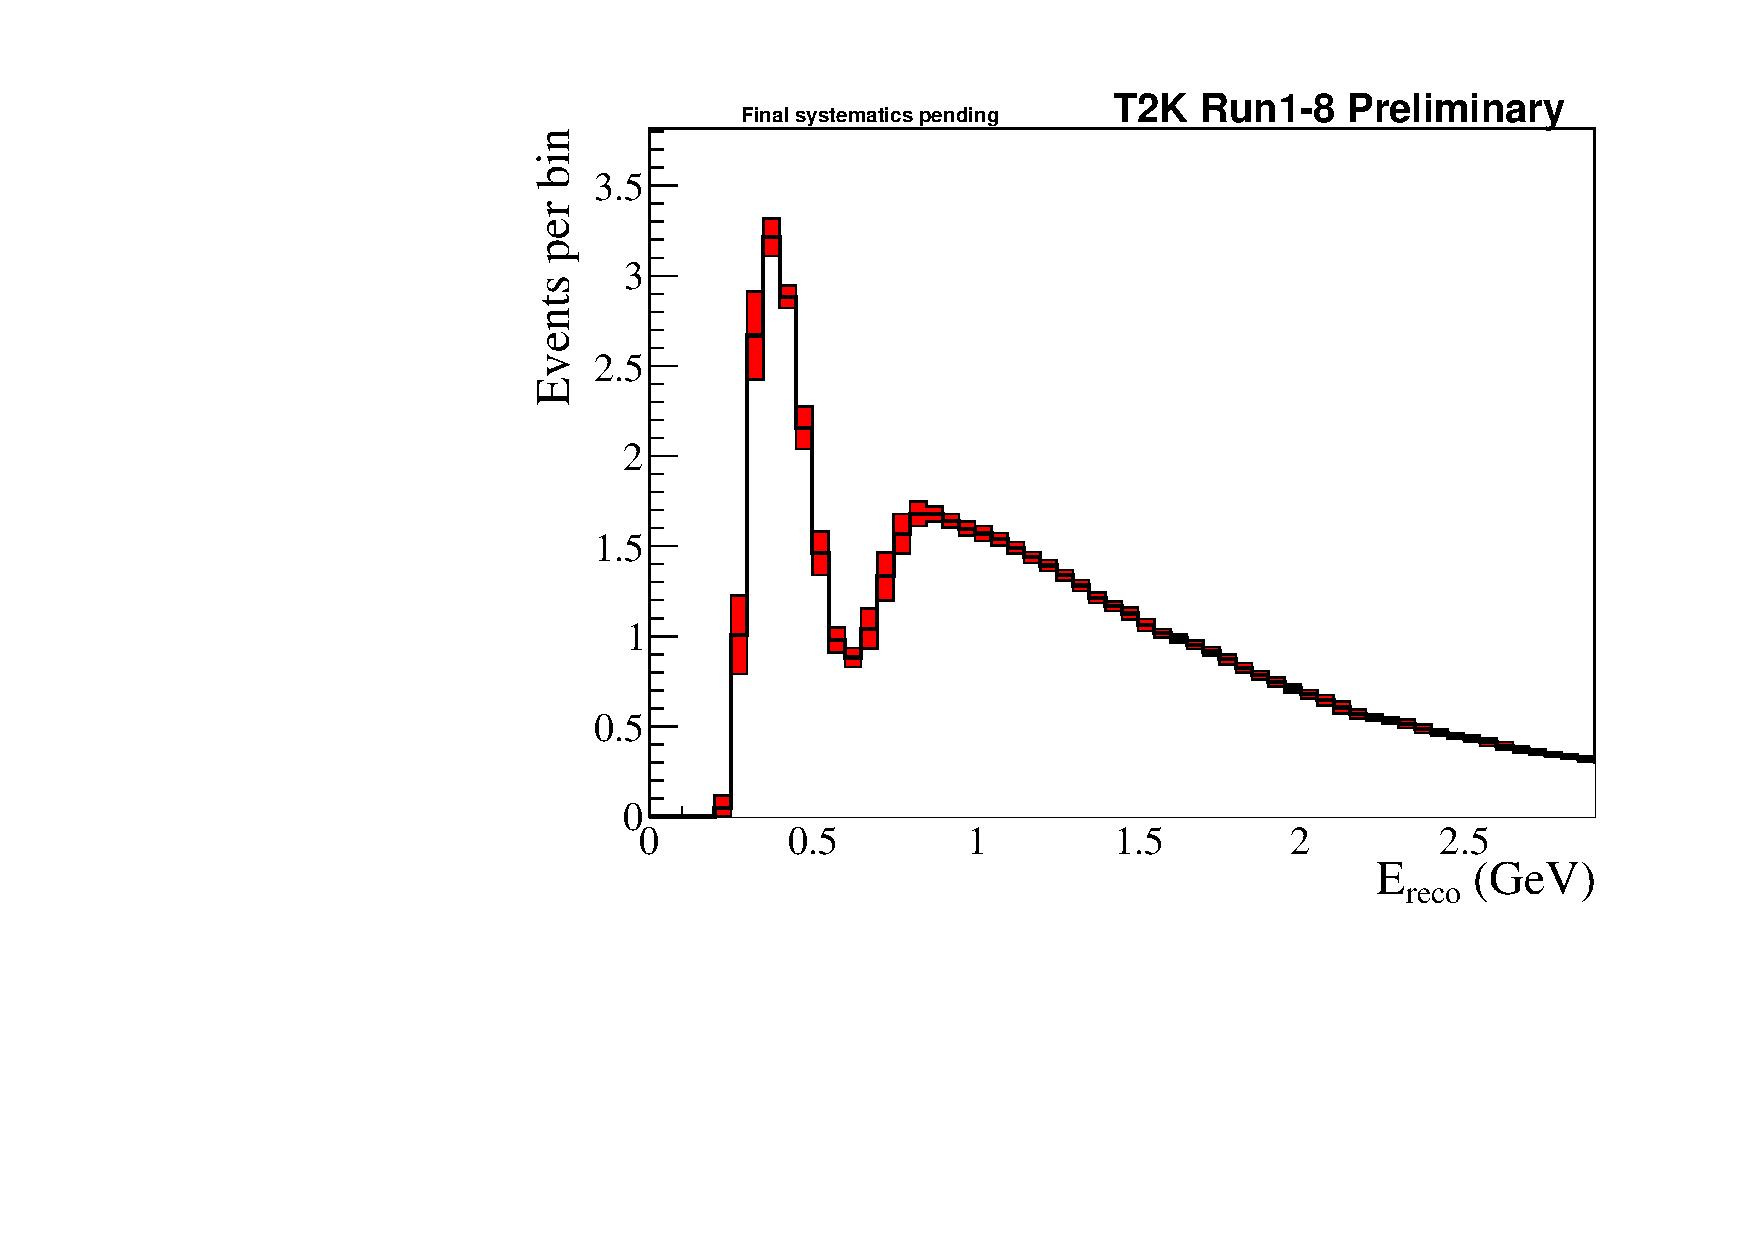
\includegraphics[width=0.9\textwidth]{systematics/envelopes/sk_errors/sk_error_table_RHC1Rmu_skfsi_envelope}
		\caption{Muon-like, antineutrino mode}
	\end{subfigure}
	\begin{subfigure}[b]{0.49\textwidth}
		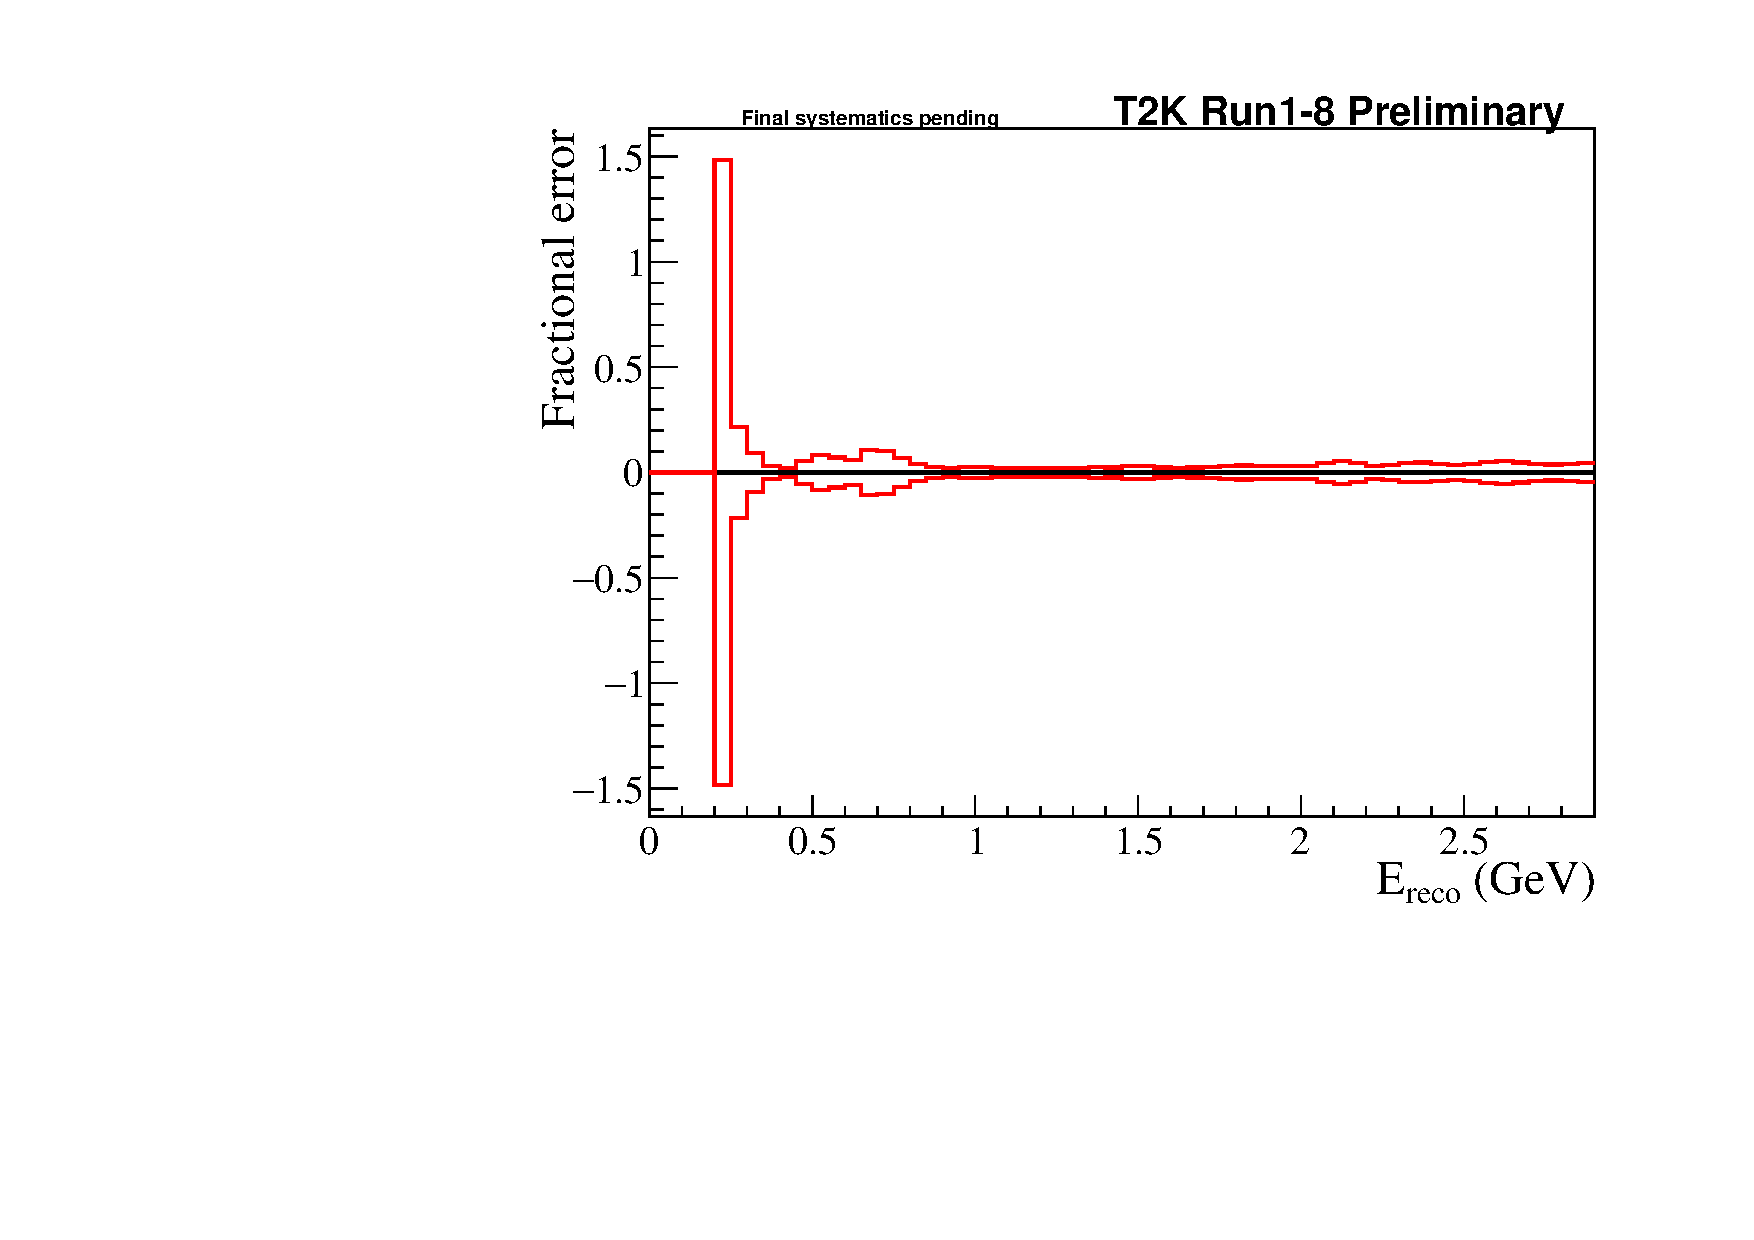
\includegraphics[width=0.9\textwidth]{systematics/envelopes/sk_errors/sk_error_table_RHC1Rmu_skfsi_envelope_fractional}
		\caption{Muon-like, antineutrino mode}
	\end{subfigure}
	\begin{subfigure}[b]{0.49\textwidth}
		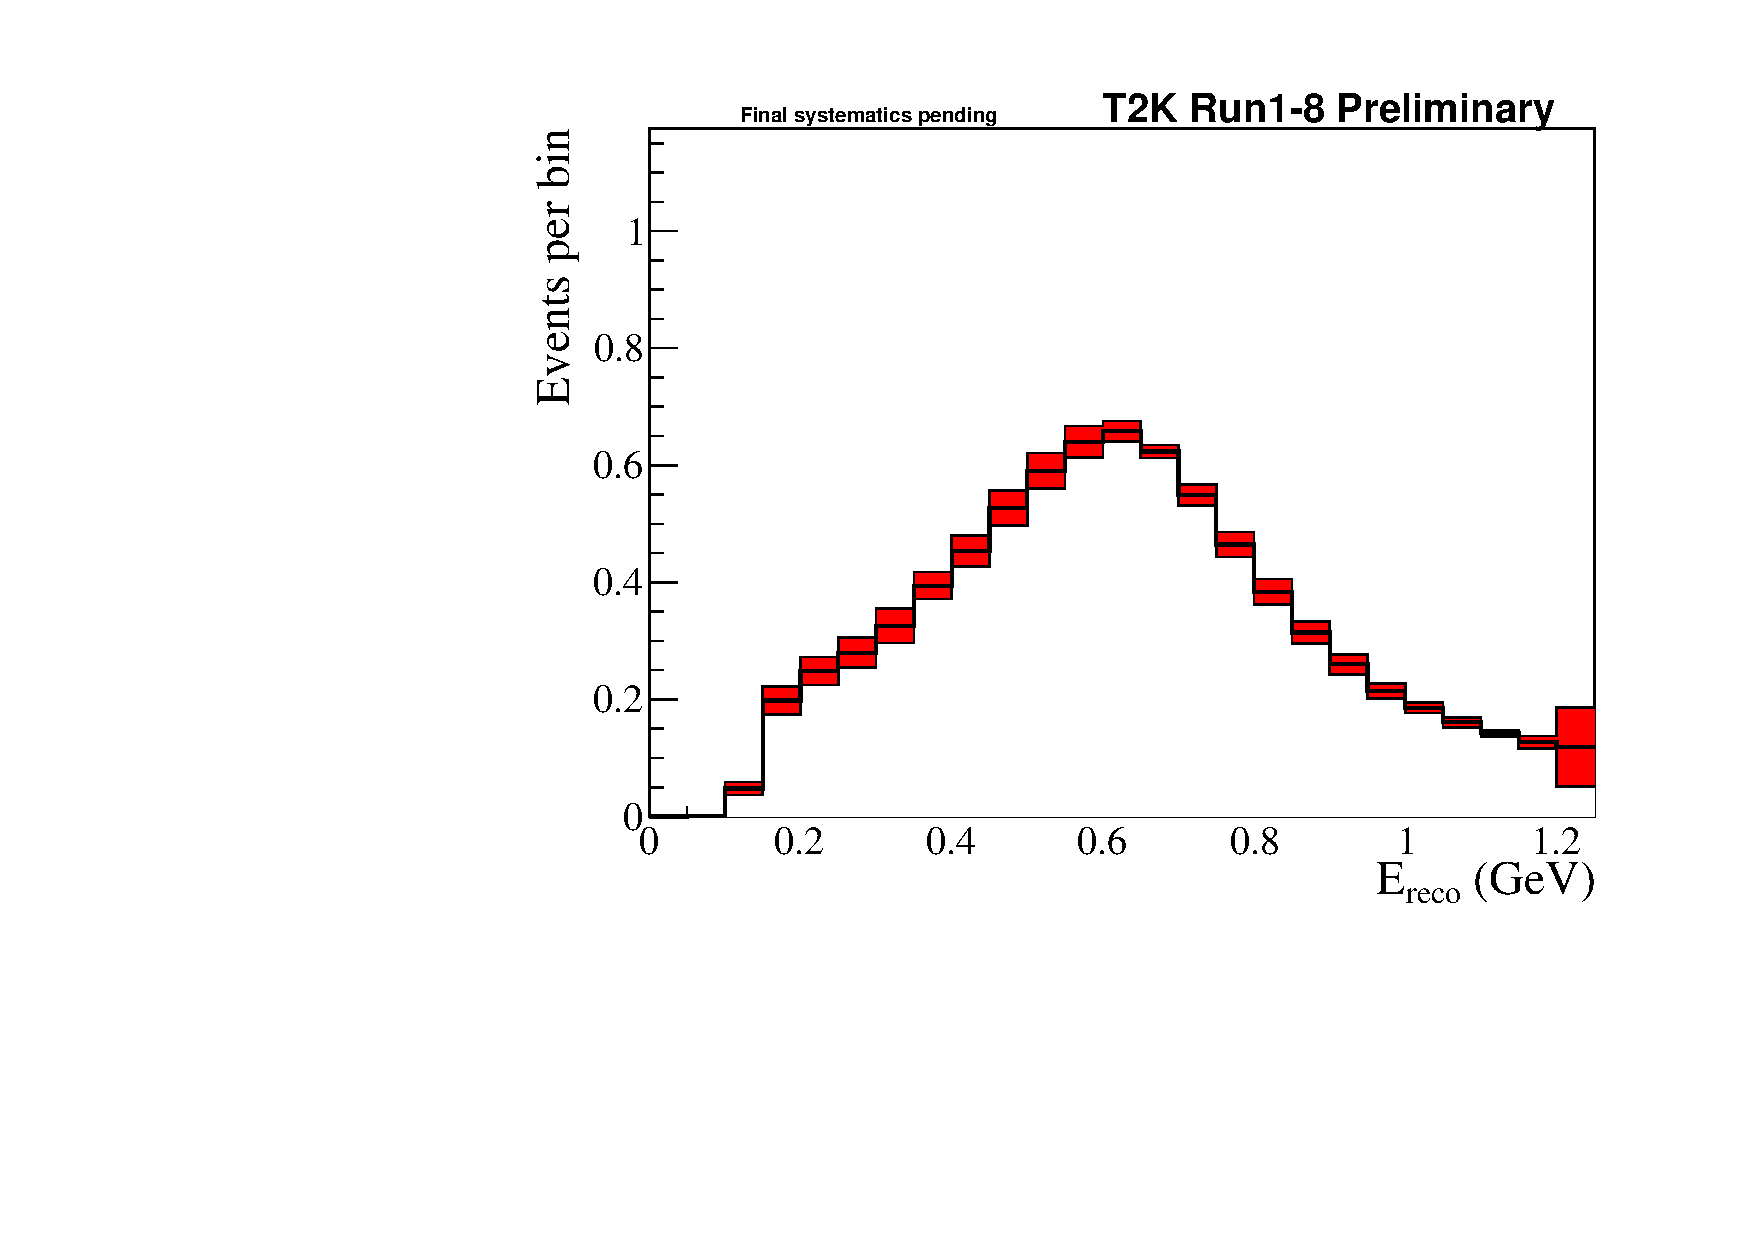
\includegraphics[width=0.9\textwidth]{systematics/envelopes/sk_errors/sk_error_table_RHC1Re_skfsi_envelope}
		\caption{Electron-like antineutrino mode}
	\end{subfigure}
	\begin{subfigure}[b]{0.49\textwidth}
		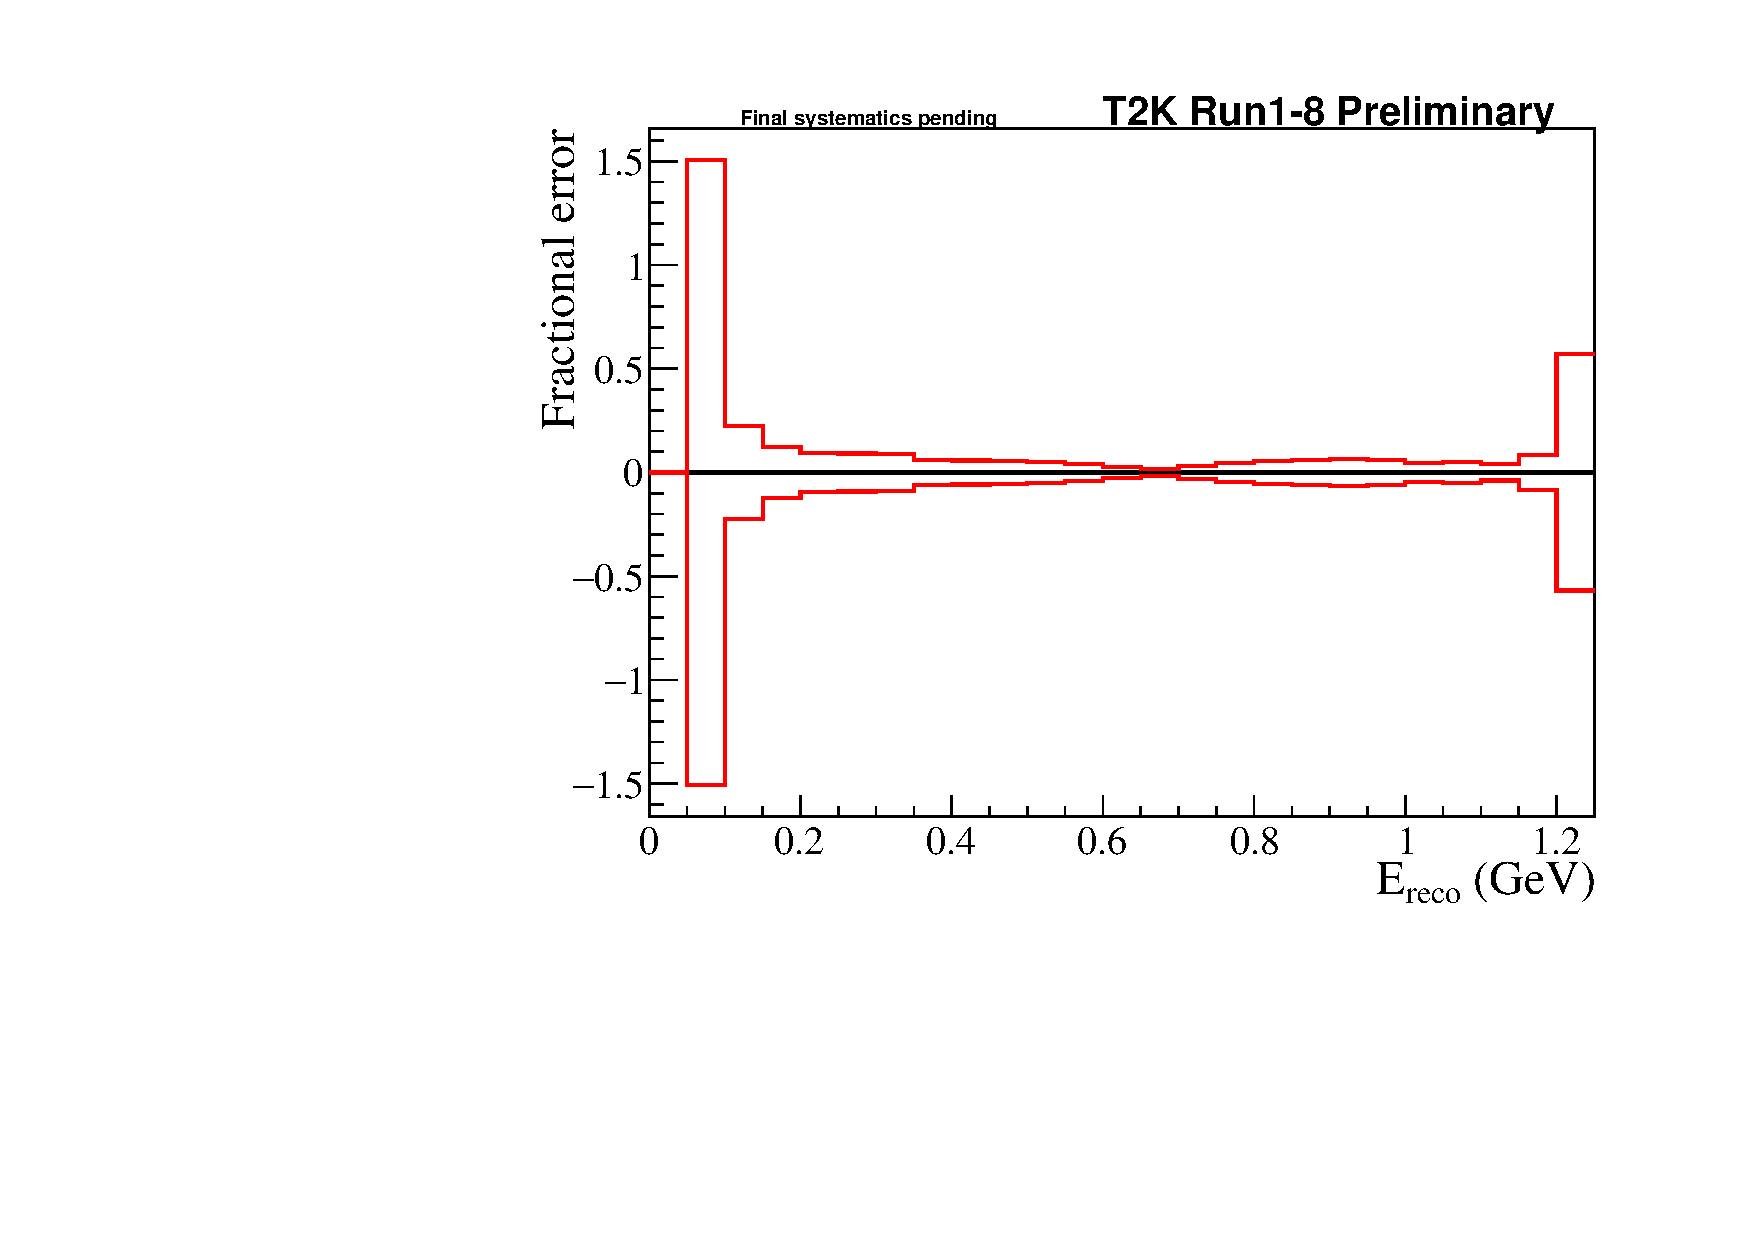
\includegraphics[width=0.9\textwidth]{systematics/envelopes/sk_errors/sk_error_table_RHC1Re_skfsi_envelope_fractional}
		\caption{Electron-like antineutrino mode}
	\end{subfigure}
	\caption {
		Error envelopes (left) and fractional errors (right) for the reconstructed neutrino energy spectrum for Super-K FSI+SI+PN systematic parameters. \num{1e4} toys are generated for the Asimov data set A with randomized systematic parameters with correlations taken into account.
	}
	\label{fig:sk_envelopes_skfsi_b}
\end{figure*}
\clearpage
\begin{figure*}
	\center
	\begin{subfigure}[b]{0.49\textwidth}
		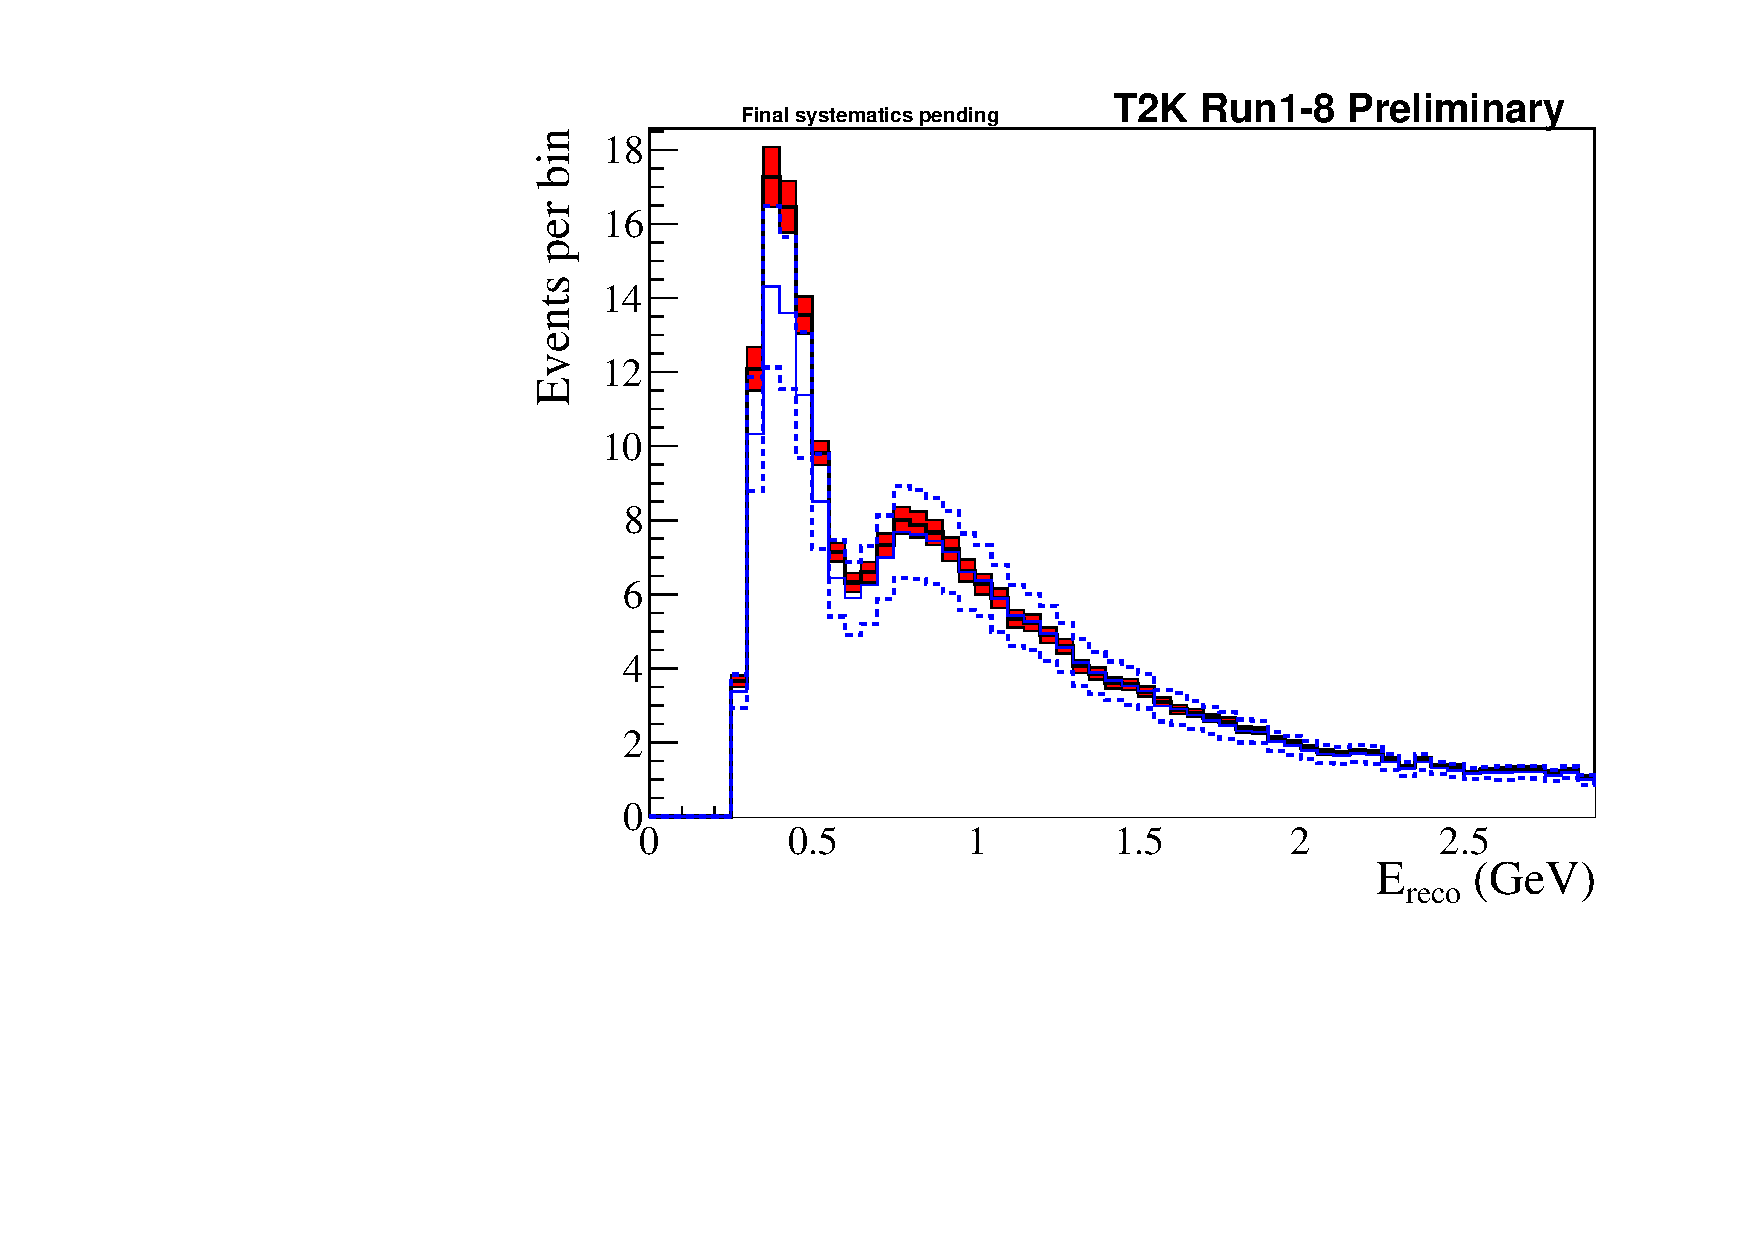
\includegraphics[width=0.9\textwidth]{systematics/envelopes/sk_errors/sk_error_table_1Rmu_banff_constrained_envelope}
		\caption{Muon-like, neutrino mode}
	\end{subfigure}
	\begin{subfigure}[b]{0.49\textwidth}
		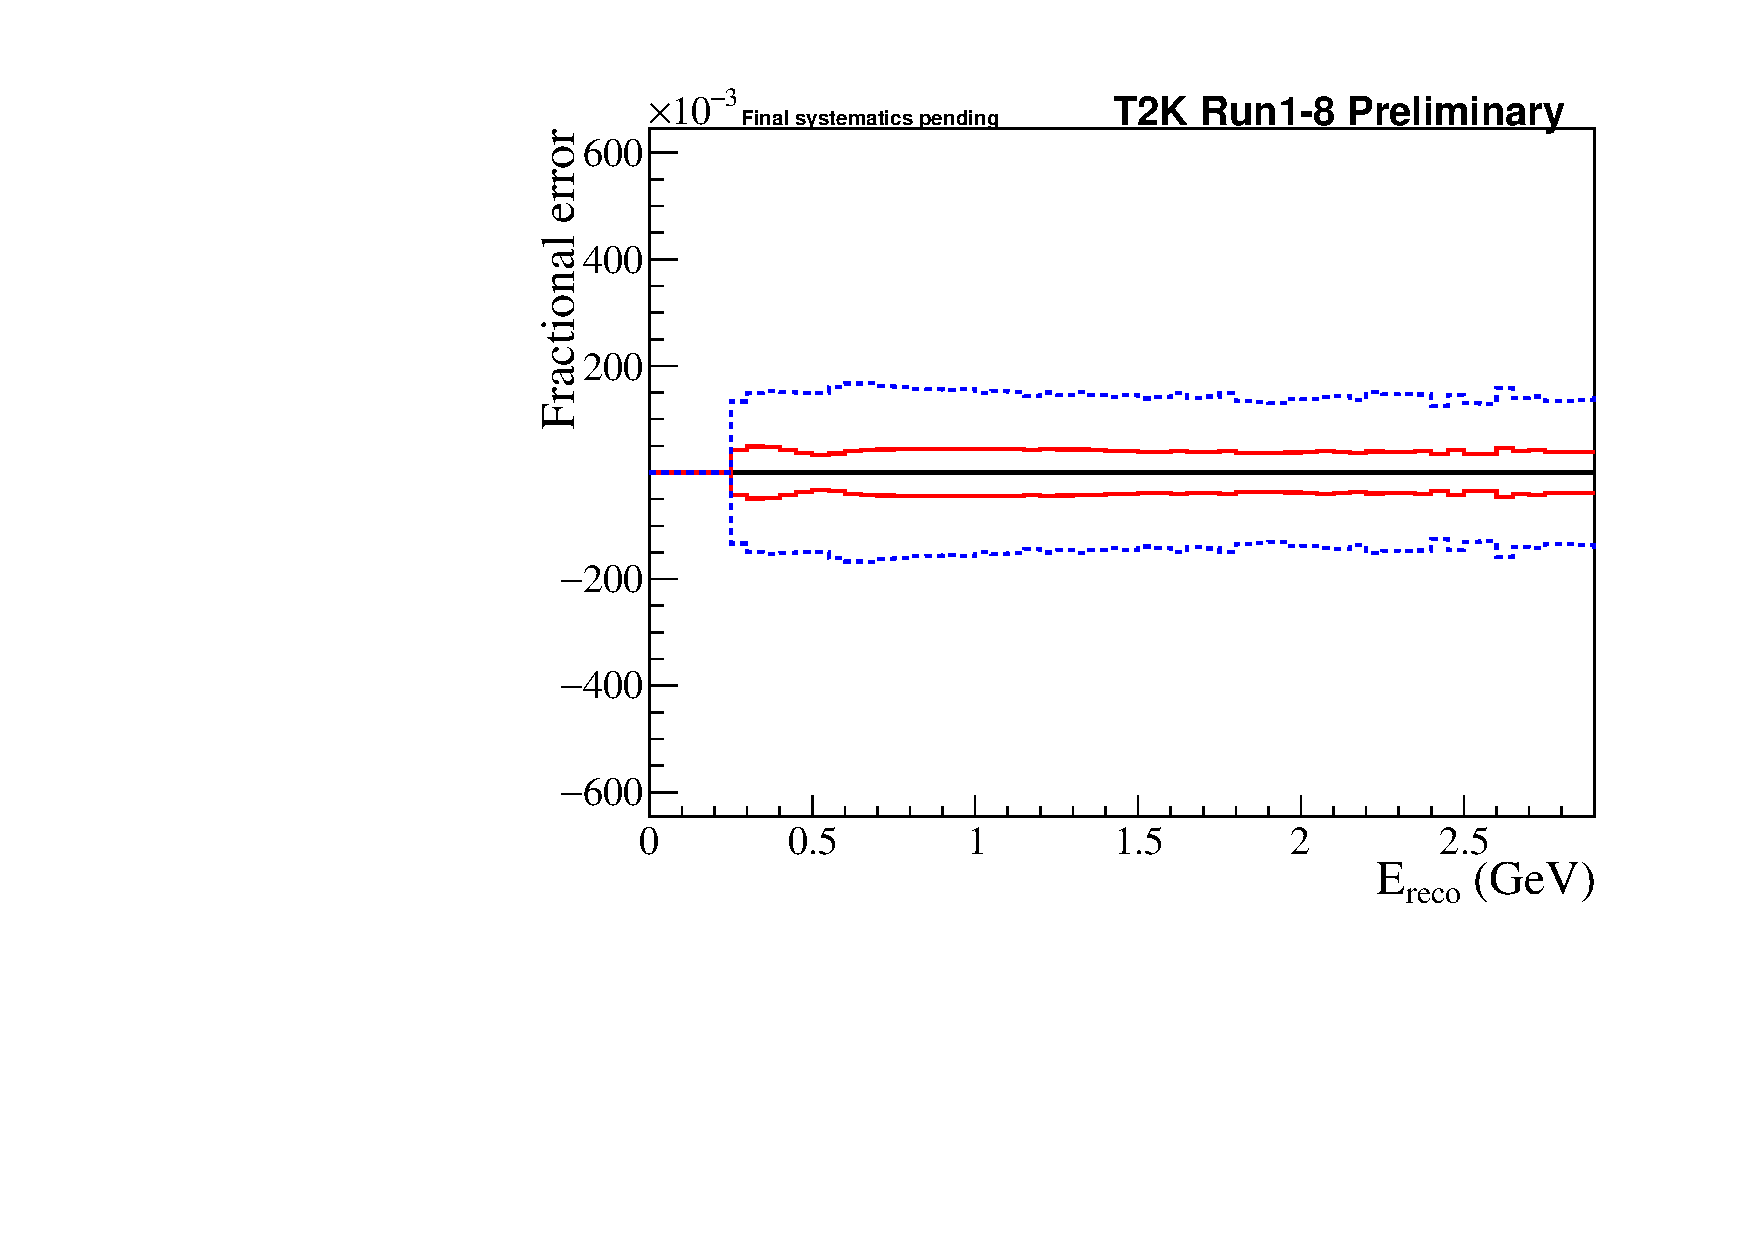
\includegraphics[width=0.9\textwidth]{systematics/envelopes/sk_errors/sk_error_table_1Rmu_banff_constrained_envelope_fractional}
		\caption{Muon-like, neutrino mode}
	\end{subfigure}
	\begin{subfigure}[b]{0.49\textwidth}
		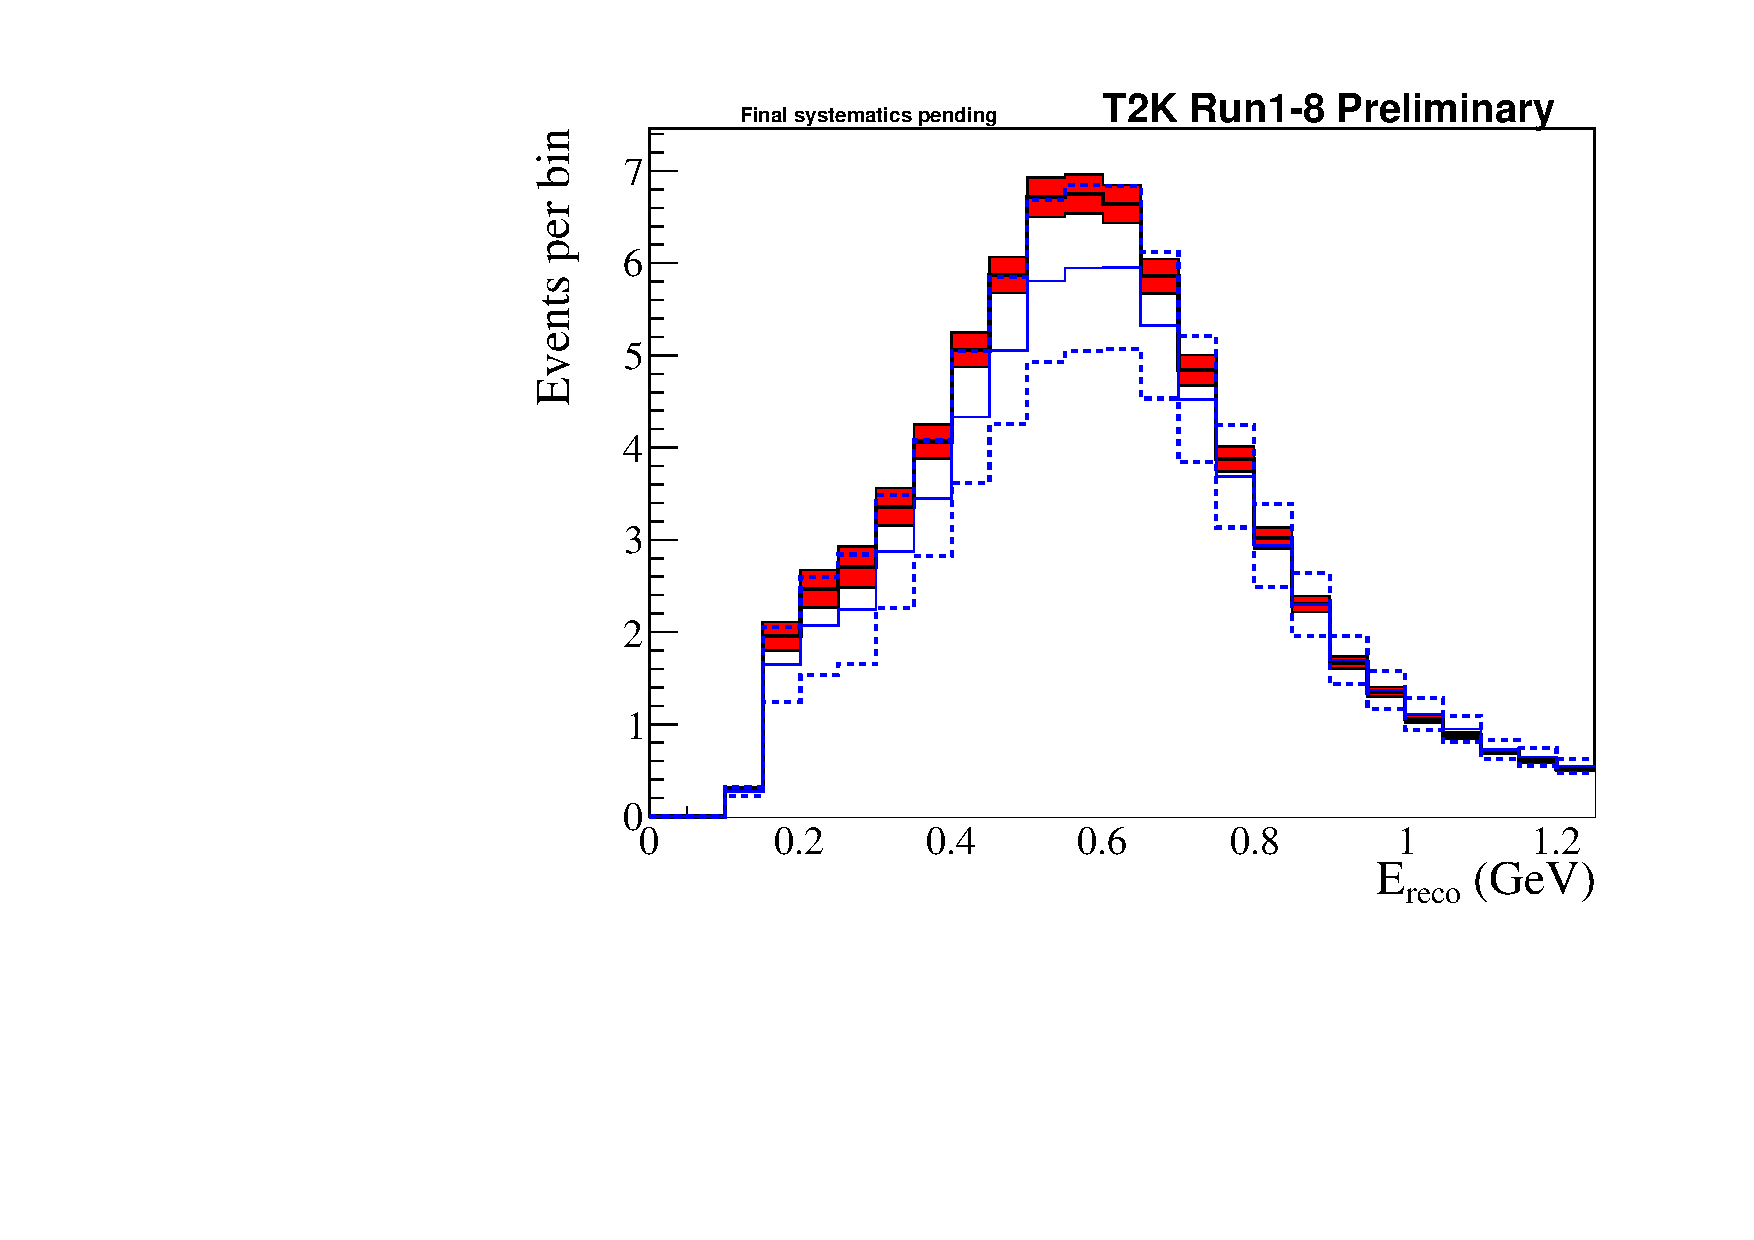
\includegraphics[width=0.9\textwidth]{systematics/envelopes/sk_errors/sk_error_table_1Re_banff_constrained_envelope}
		\caption{Electron-like, neutrino mode}
	\end{subfigure}
	\begin{subfigure}[b]{0.49\textwidth}
		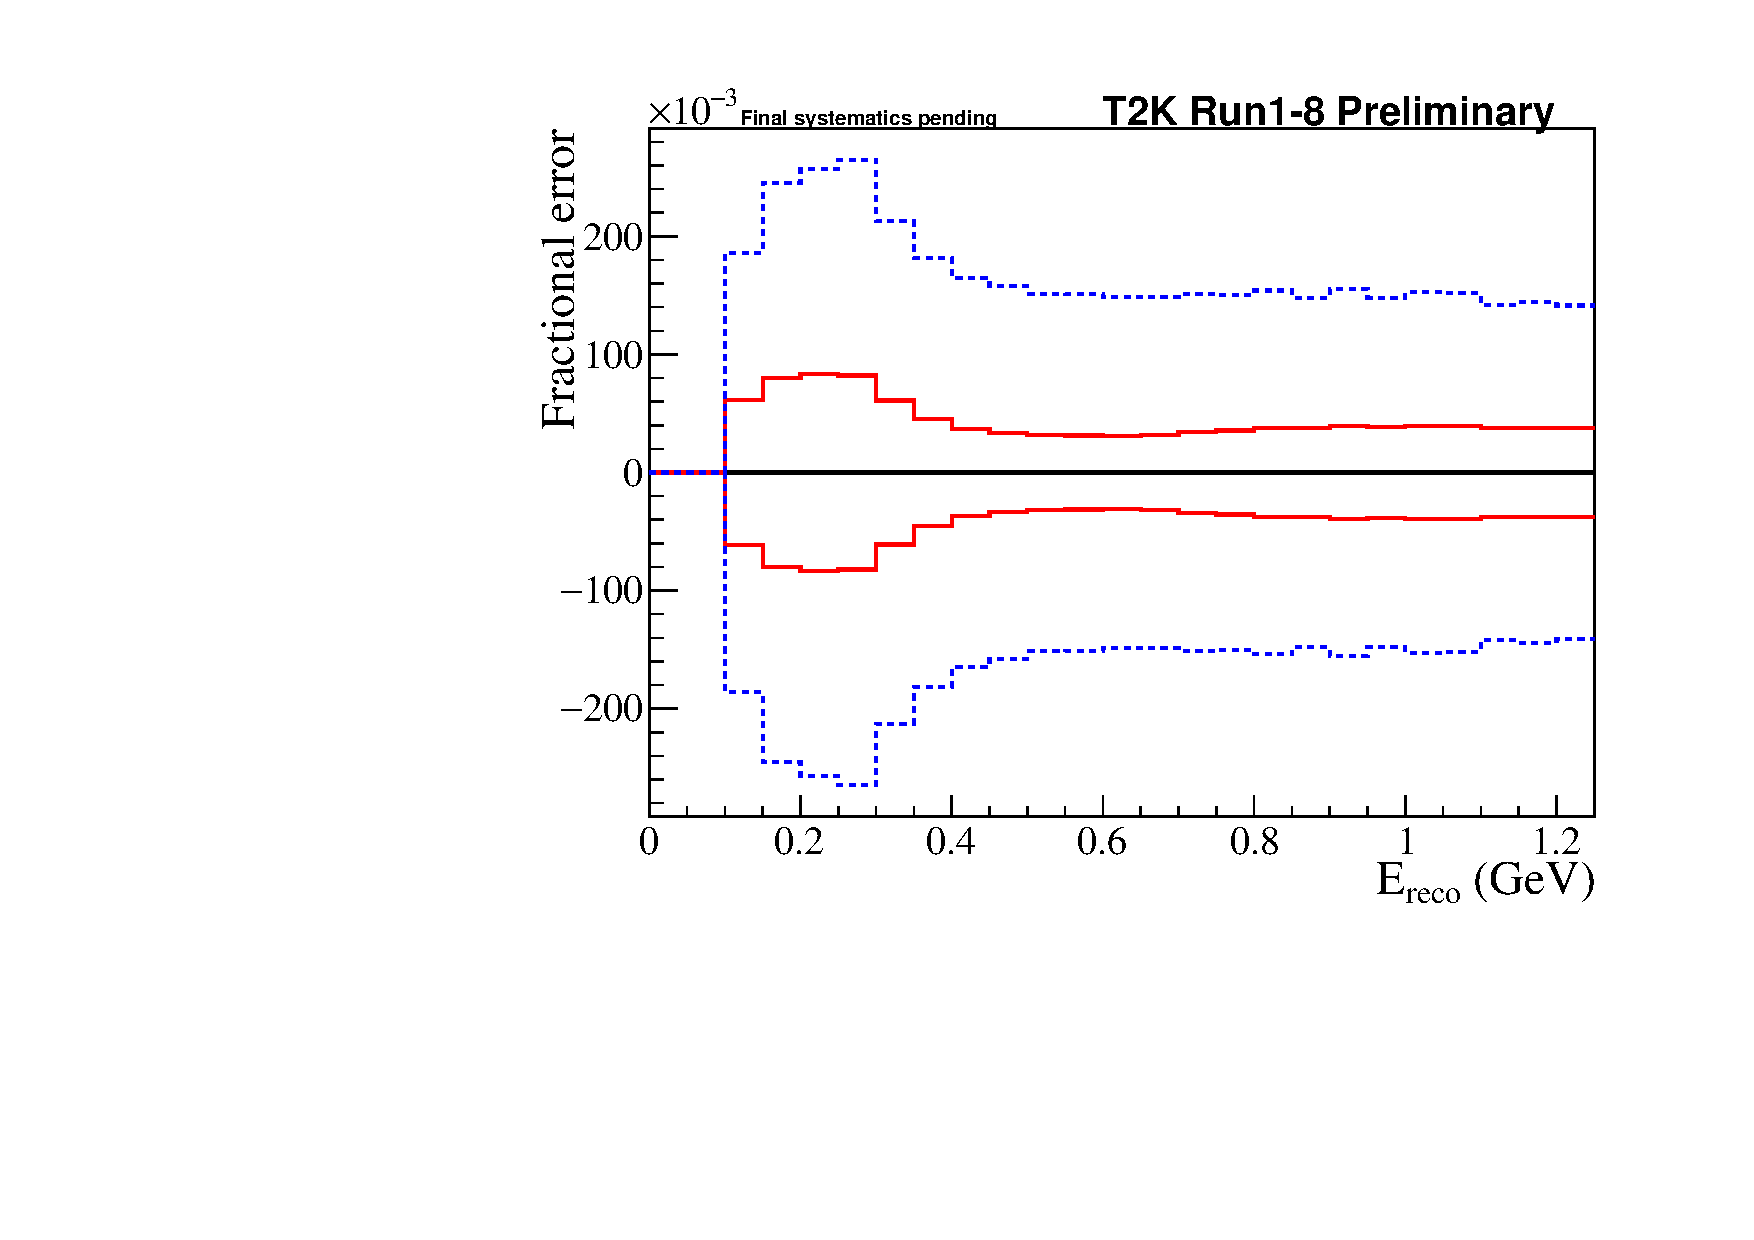
\includegraphics[width=0.9\textwidth]{systematics/envelopes/sk_errors/sk_error_table_1Re_banff_constrained_envelope_fractional}
		\caption{Electron-like, neutrino mode}
	\end{subfigure}
	\begin{subfigure}[b]{0.49\textwidth}
		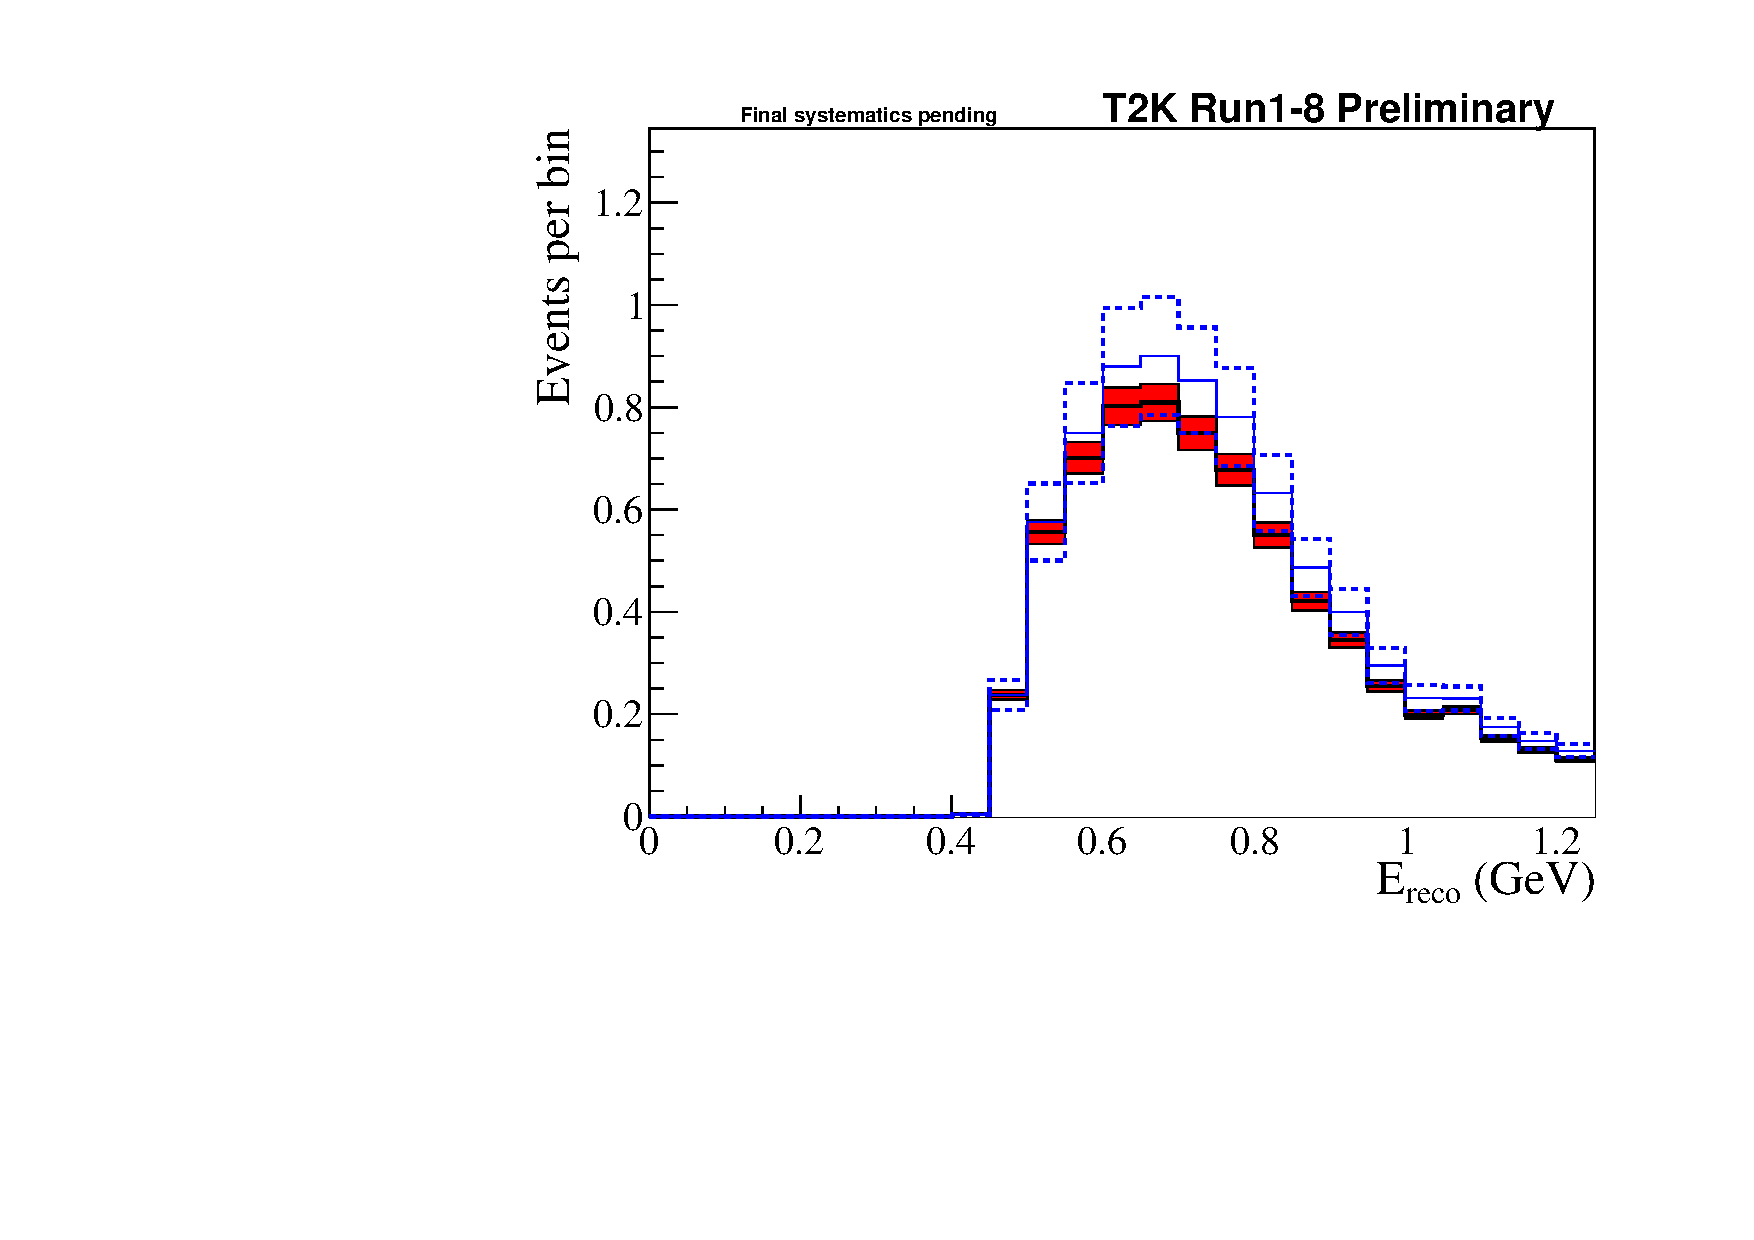
\includegraphics[width=0.9\textwidth]{systematics/envelopes/sk_errors/sk_error_table_MultiRe_banff_constrained_envelope}
		\caption{\nueCConepi-like, neutrino mode}
	\end{subfigure}
	\begin{subfigure}[b]{0.49\textwidth}
		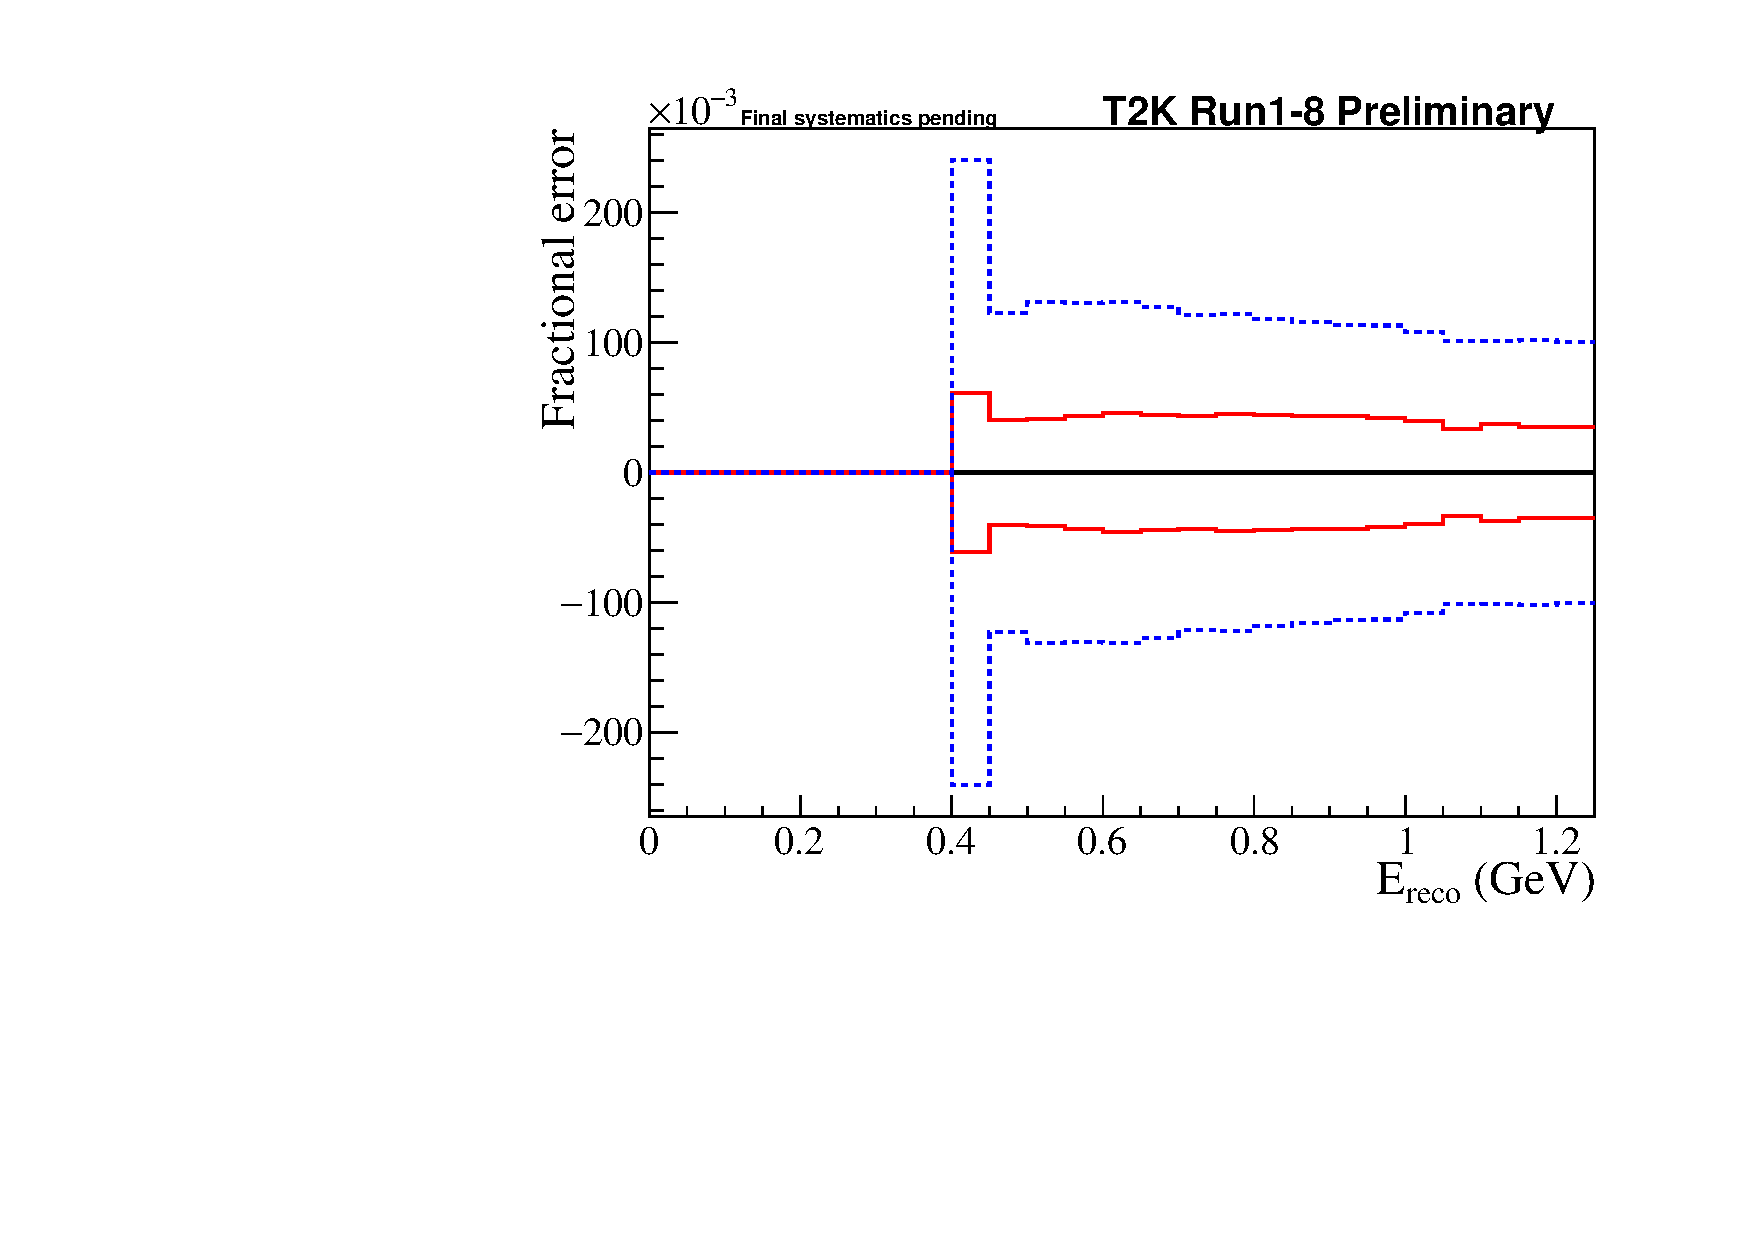
\includegraphics[width=0.9\textwidth]{systematics/envelopes/sk_errors/sk_error_table_MultiRe_banff_constrained_envelope_fractional}
		\caption{\nueCConepi-like, neutrino mode}
	\end{subfigure}
	\caption {
		Error envelopes (left) and fractional errors (right) for the reconstructed neutrino energy spectrum for the flux and constrained cross-section systematic parameters for pre-BANFF (blue) and post-BANFF (red) errors. \num{1e4} toys are generated for the Asimov data set A with randomized systematic parameters with correlations taken into account.
	}
	\label{fig:sk_envelopes_banff}
\end{figure*}
\clearpage

\begin{figure*}
	\center
	\begin{subfigure}[b]{0.49\textwidth}
		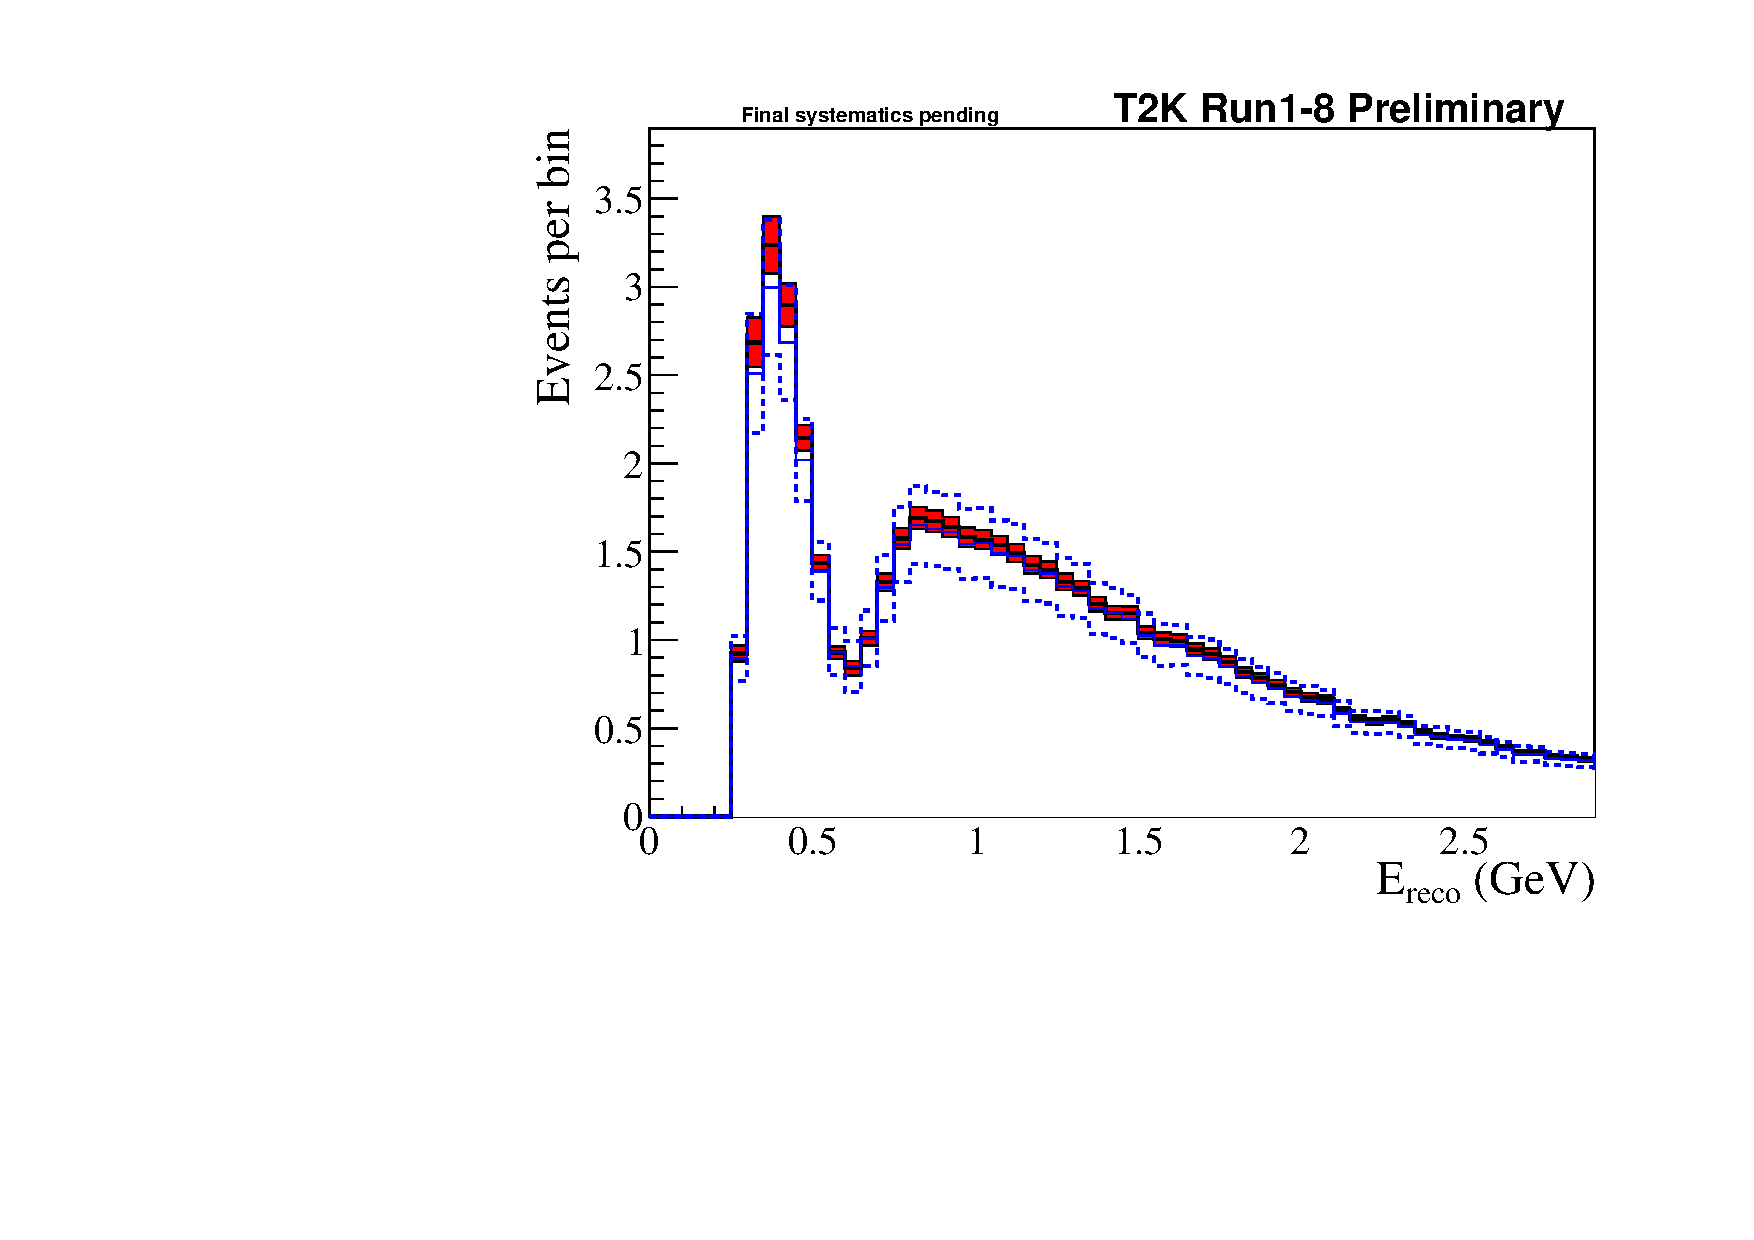
\includegraphics[width=0.9\textwidth]{systematics/envelopes/sk_errors/sk_error_table_RHC1Rmu_banff_constrained_envelope}
		\caption{Muon-like, antineutrino mode}
	\end{subfigure}
	\begin{subfigure}[b]{0.49\textwidth}
		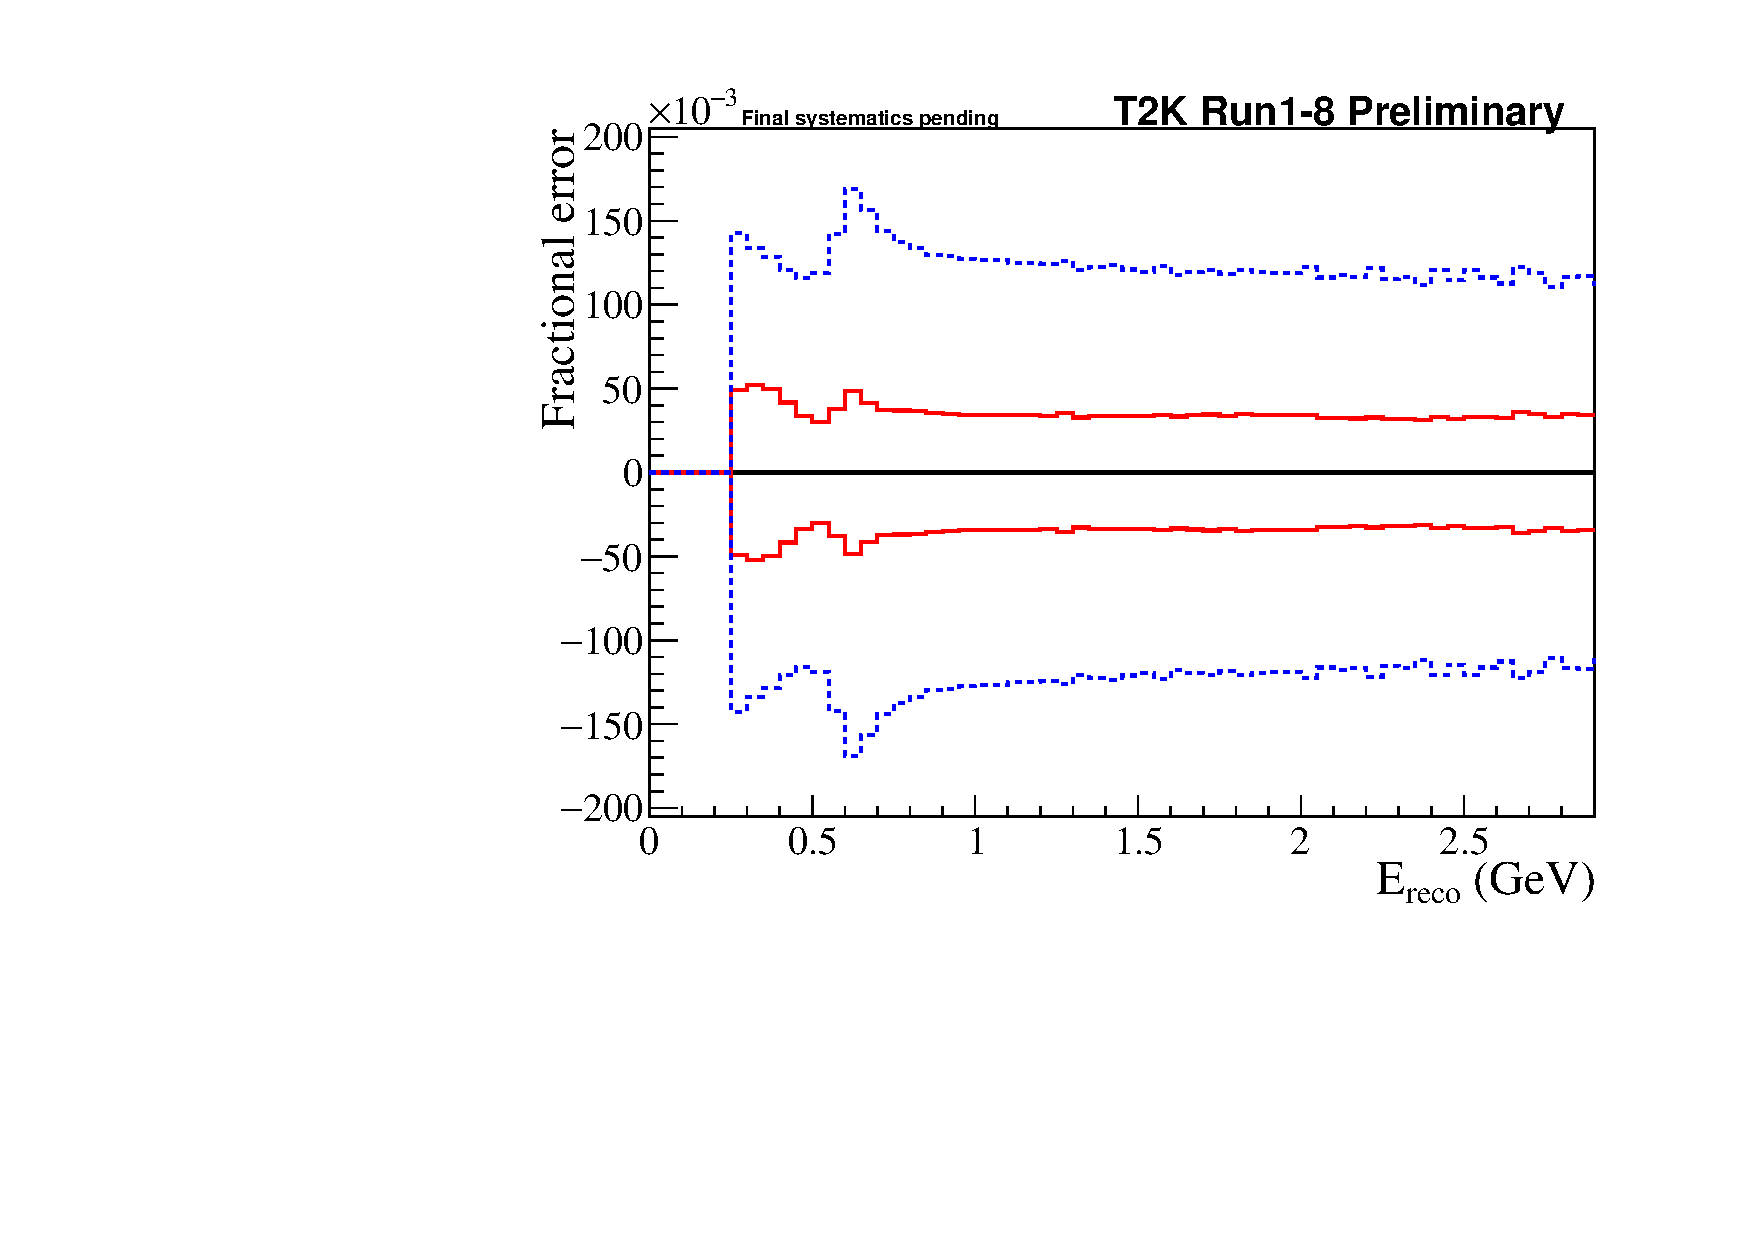
\includegraphics[width=0.9\textwidth]{systematics/envelopes/sk_errors/sk_error_table_RHC1Rmu_banff_constrained_envelope_fractional}
		\caption{Muon-like, antineutrino mode}
	\end{subfigure}
	\begin{subfigure}[b]{0.49\textwidth}
		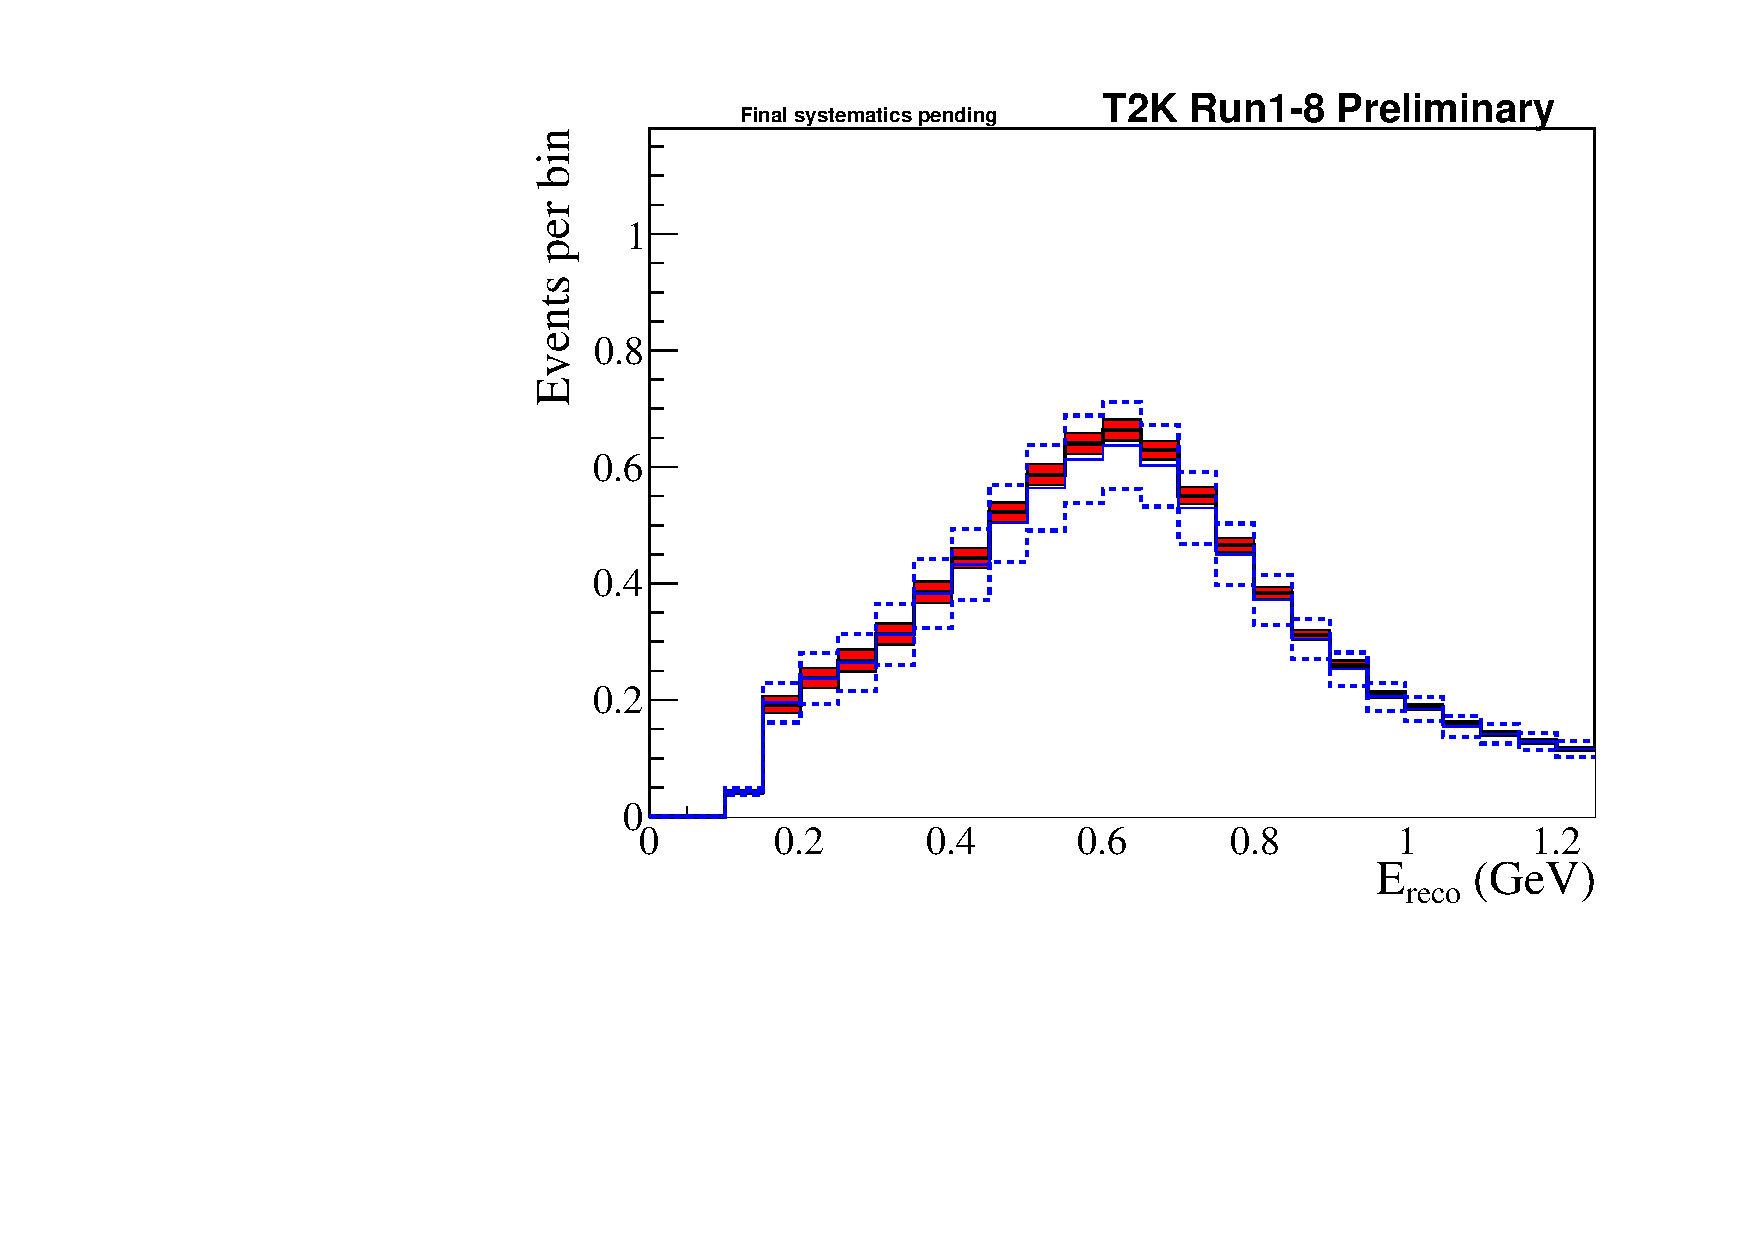
\includegraphics[width=0.9\textwidth]{systematics/envelopes/sk_errors/sk_error_table_RHC1Re_banff_constrained_envelope}
		\caption{Electron-like antineutrino mode}
	\end{subfigure}
	\begin{subfigure}[b]{0.49\textwidth}
		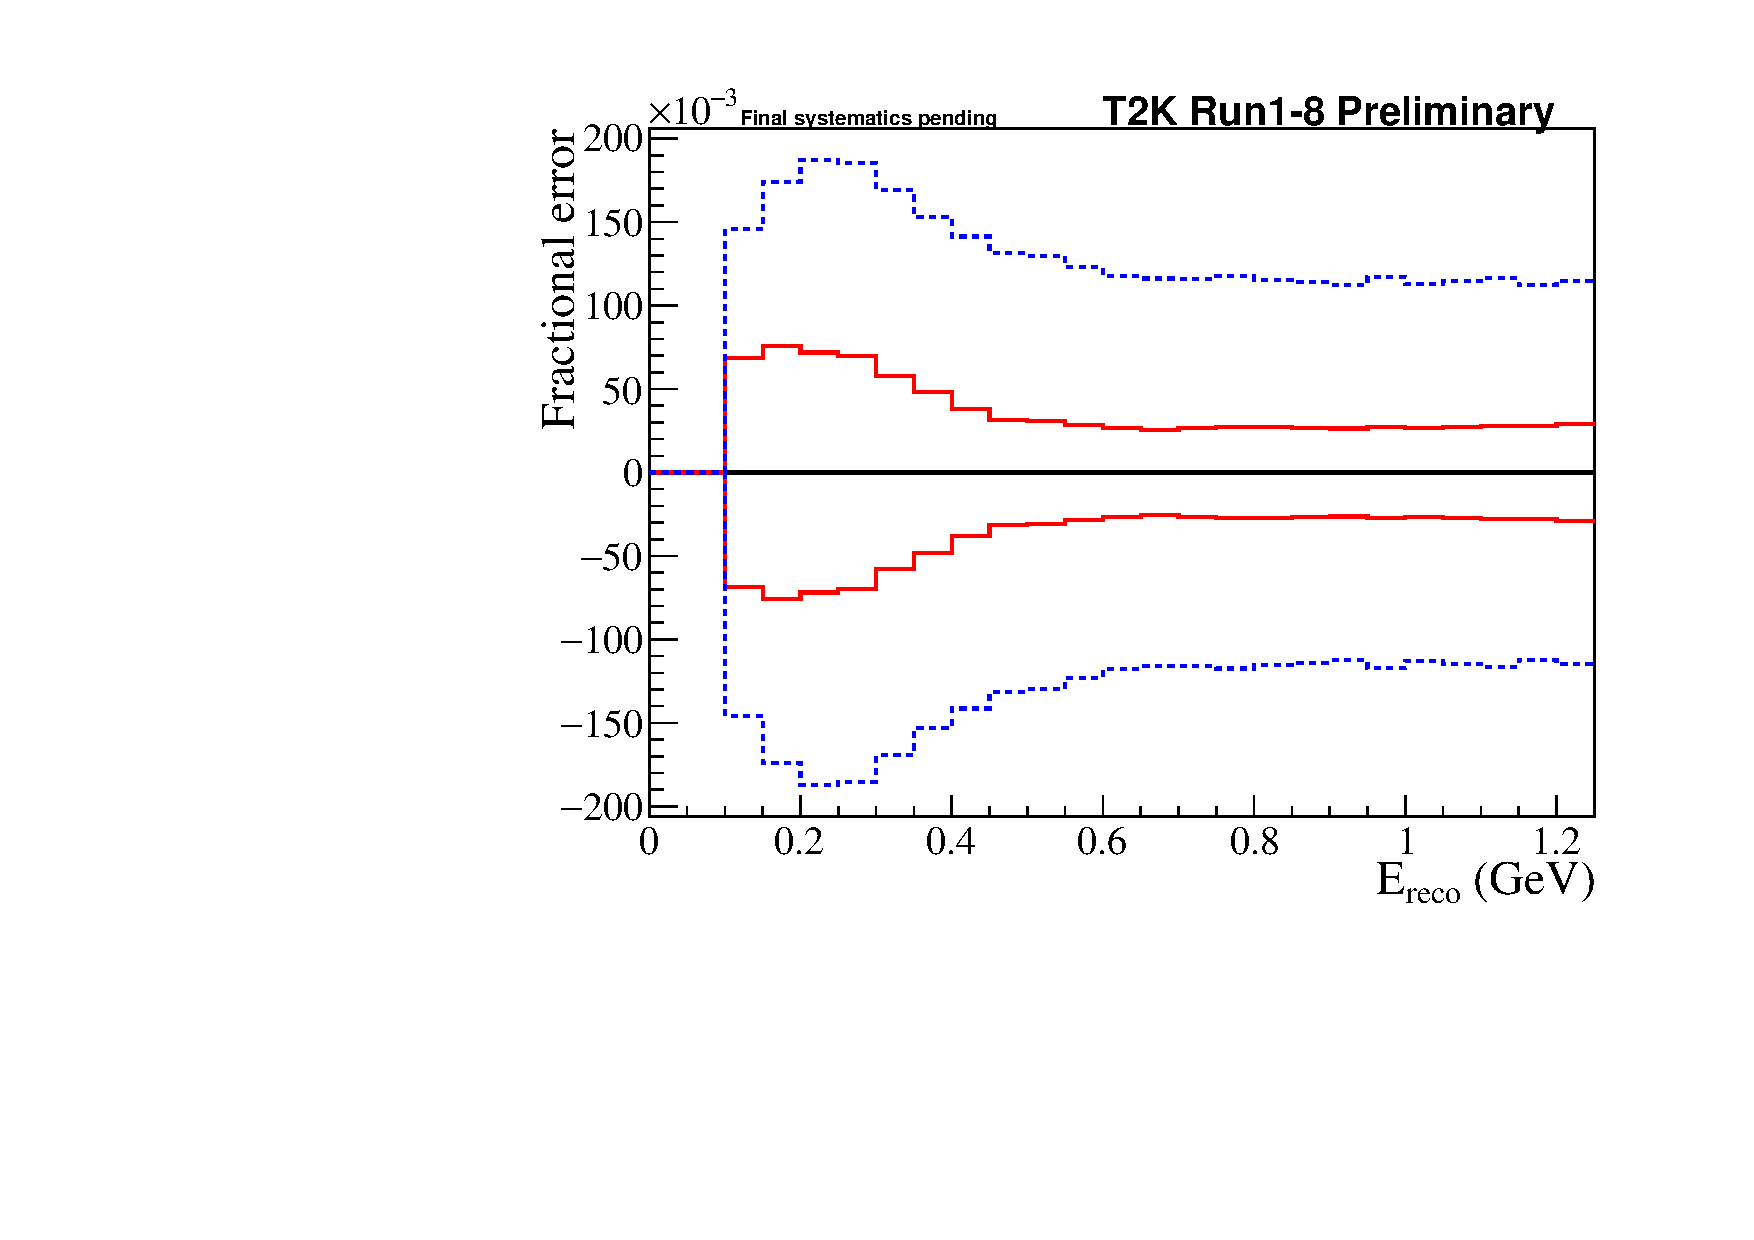
\includegraphics[width=0.9\textwidth]{systematics/envelopes/sk_errors/sk_error_table_RHC1Re_banff_constrained_envelope_fractional}
		\caption{Electron-like antineutrino mode}
	\end{subfigure}
	\caption {
		Error envelopes (left) and fractional error (right) for the reconstructed neutrino energy spectrum for the flux and constrained cross-section systematic parameters for pre-BANFF (blue) and post-BANFF (red) errors. \num{1e4} toys are generated for the Asimov data set A with randomized systematic parameters with correlations taken into account.
	}
	\label{fig:sk_envelopes_banff_b}
\end{figure*}
\clearpage
\begin{figure*}
	\center
	\begin{subfigure}[b]{0.49\textwidth}
		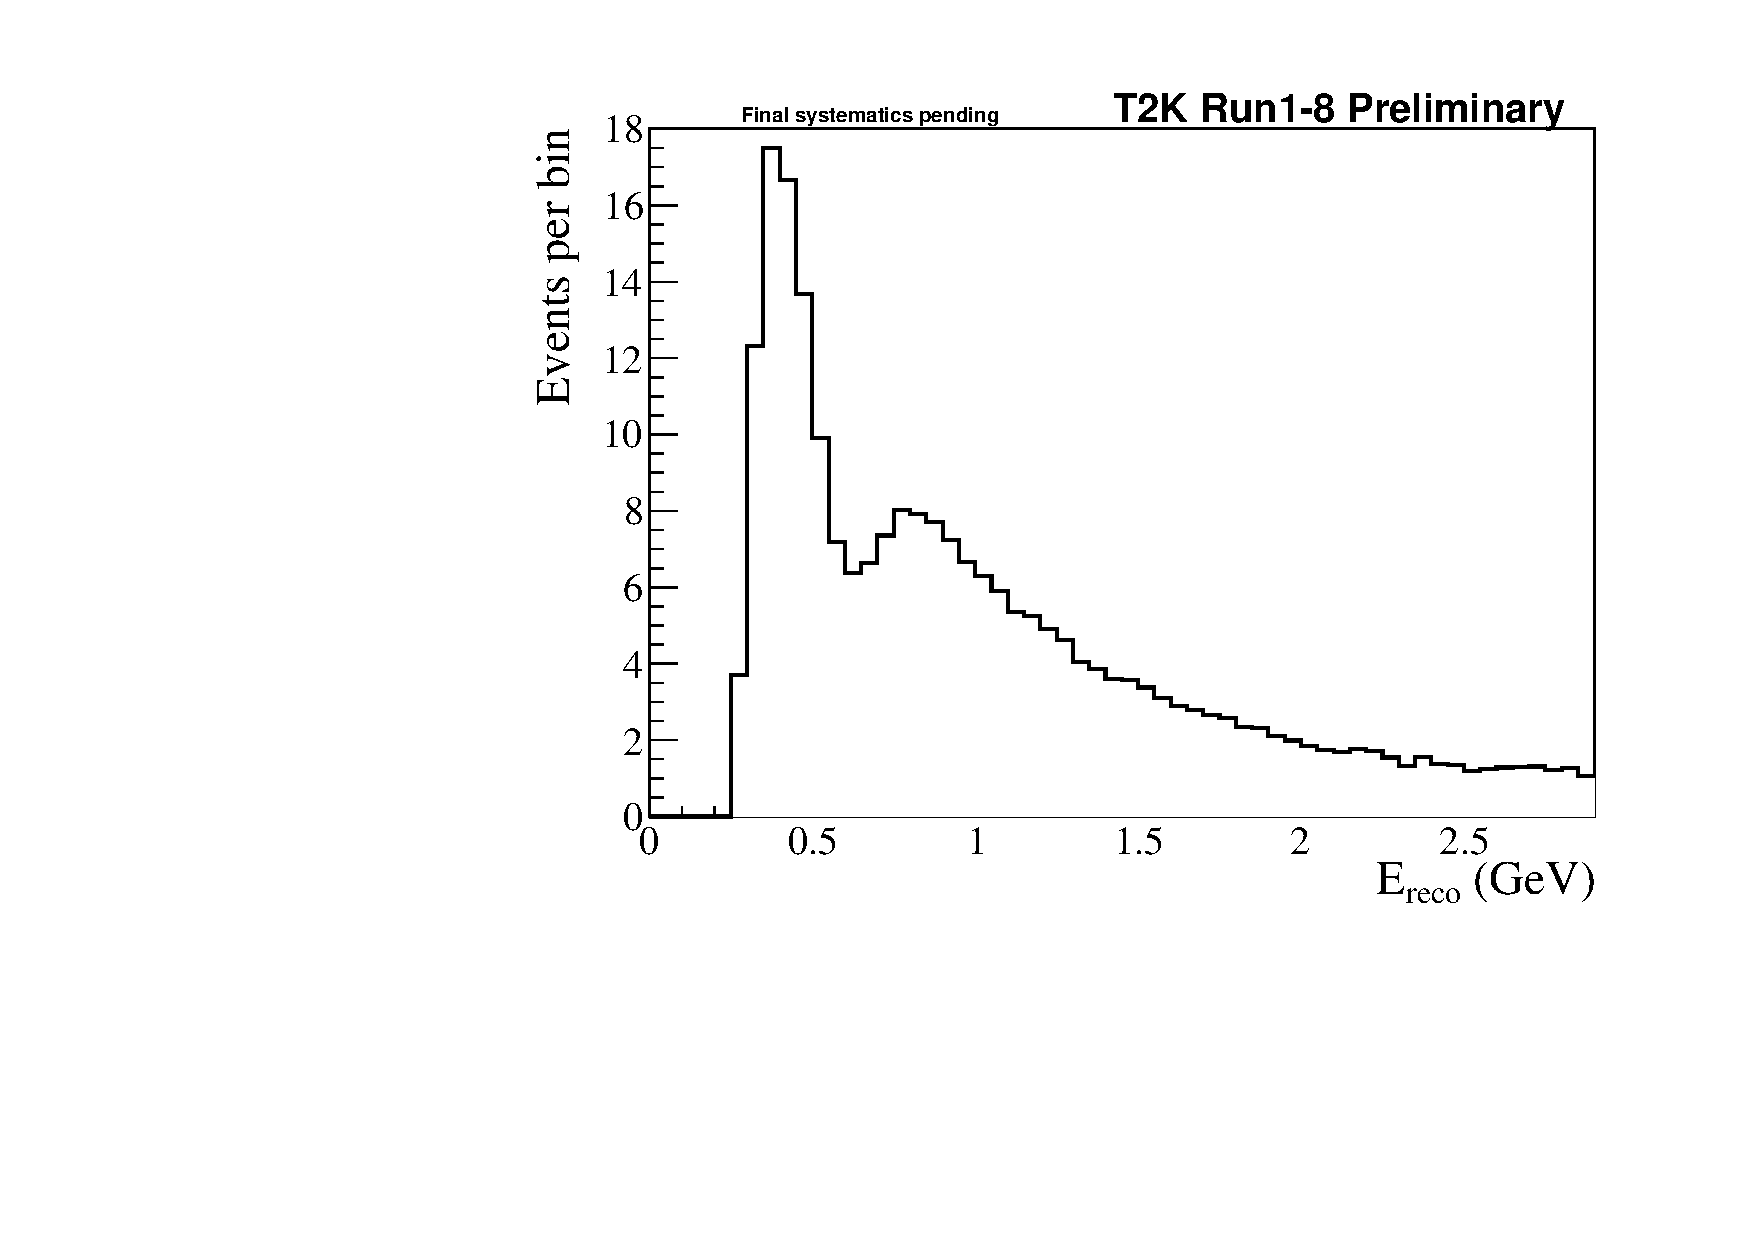
\includegraphics[width=0.9\textwidth]{systematics/envelopes/sk_errors/sk_error_table_1Rmu_xsec_nue_envelope}
		\caption{Muon-like, neutrino mode}
	\end{subfigure}
	\begin{subfigure}[b]{0.49\textwidth}
		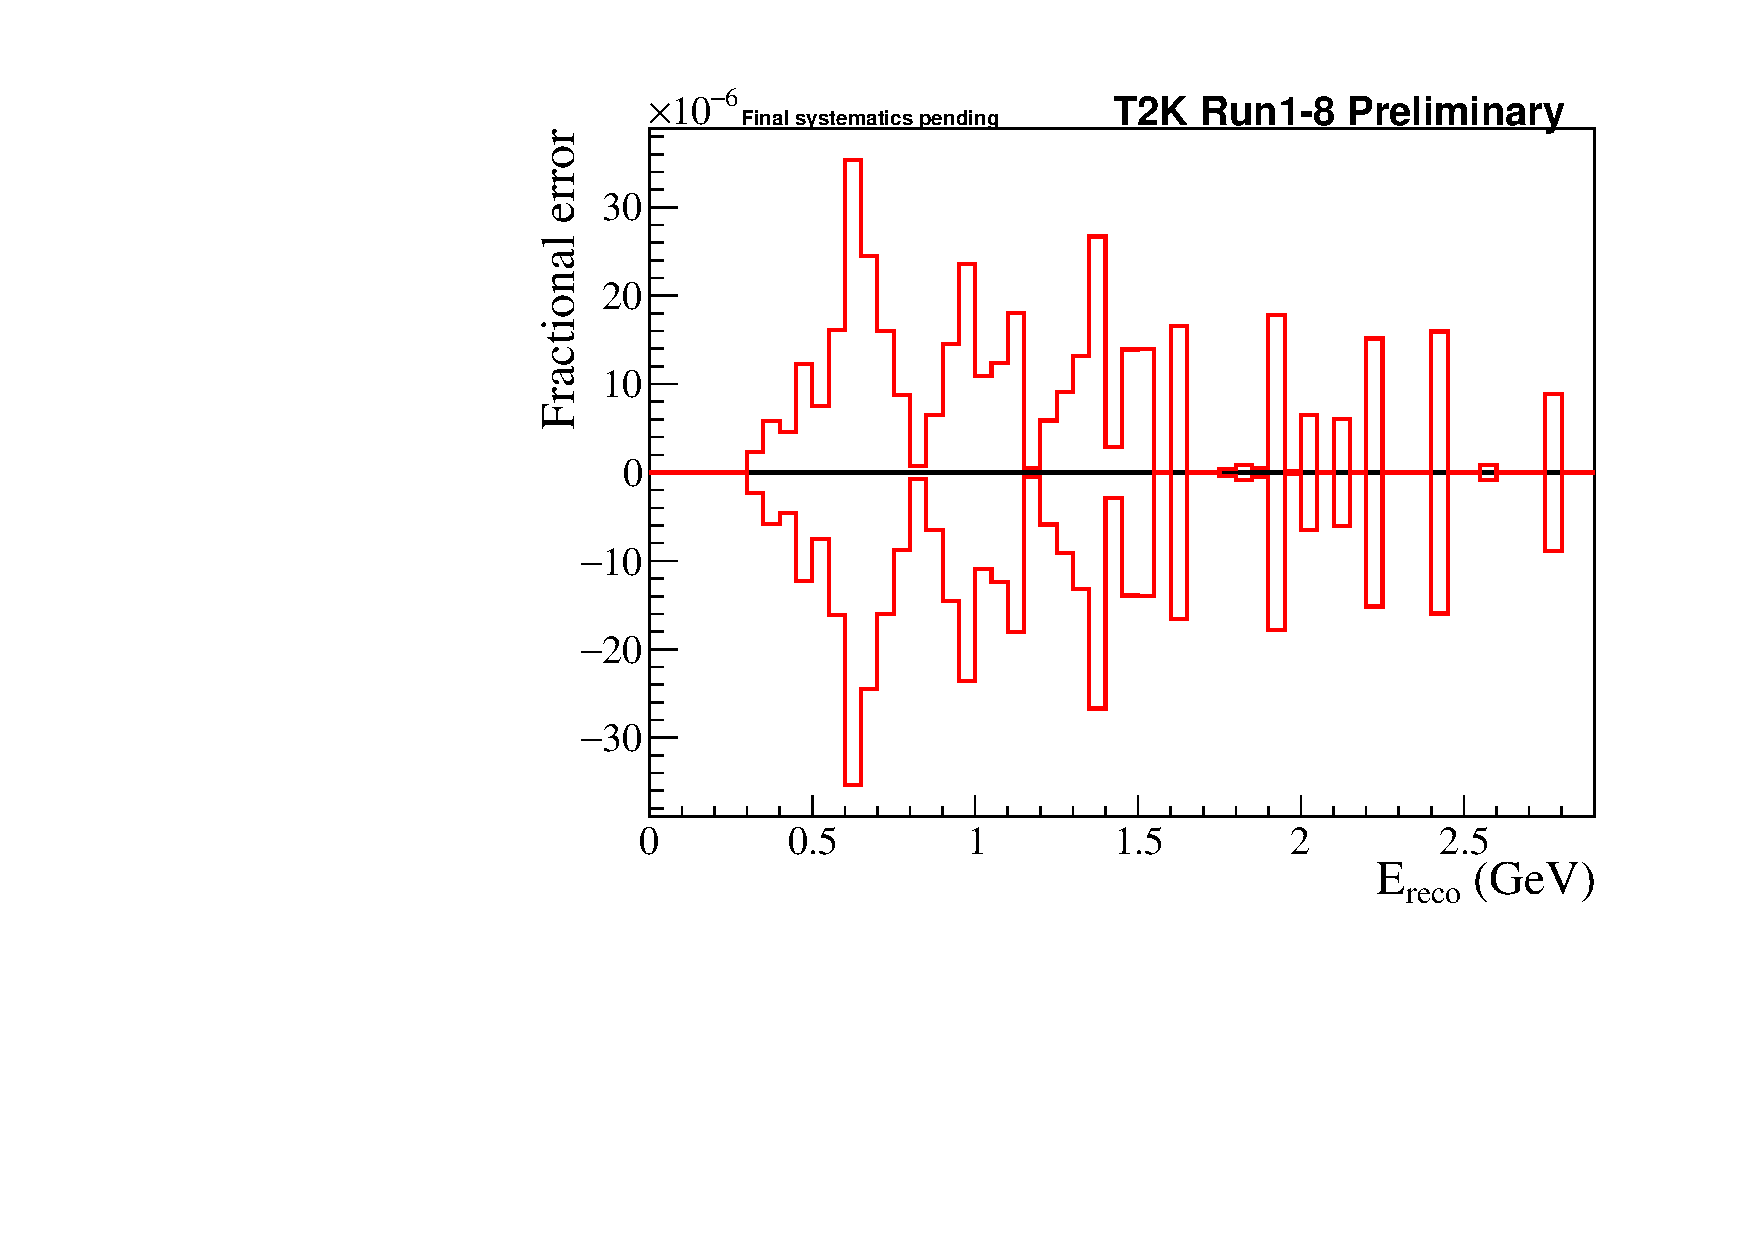
\includegraphics[width=0.9\textwidth]{systematics/envelopes/sk_errors/sk_error_table_1Rmu_xsec_nue_envelope_fractional}
		\caption{Muon-like, neutrino mode}
	\end{subfigure}
	\begin{subfigure}[b]{0.49\textwidth}
		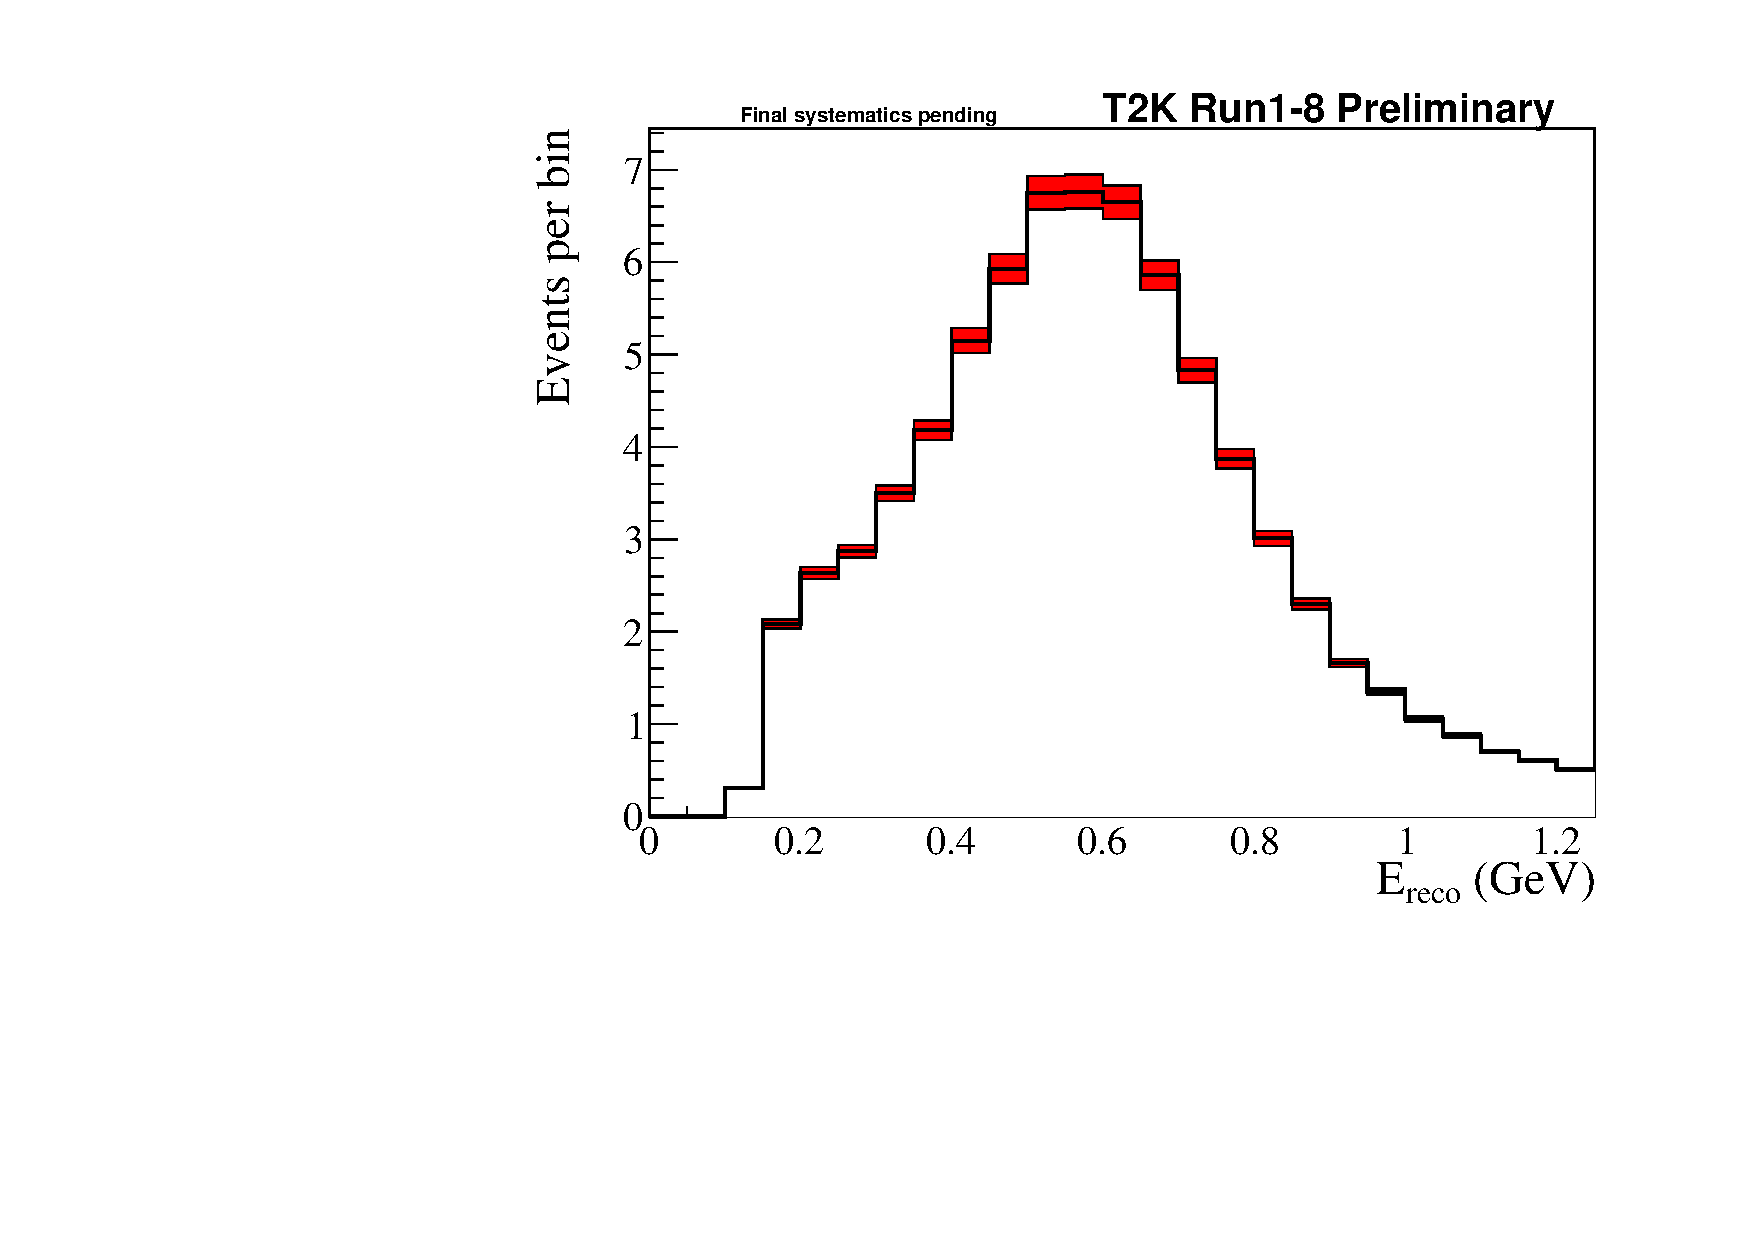
\includegraphics[width=0.9\textwidth]{systematics/envelopes/sk_errors/sk_error_table_1Re_xsec_nue_envelope}
		\caption{Electron-like, neutrino mode}
	\end{subfigure}
	\begin{subfigure}[b]{0.49\textwidth}
		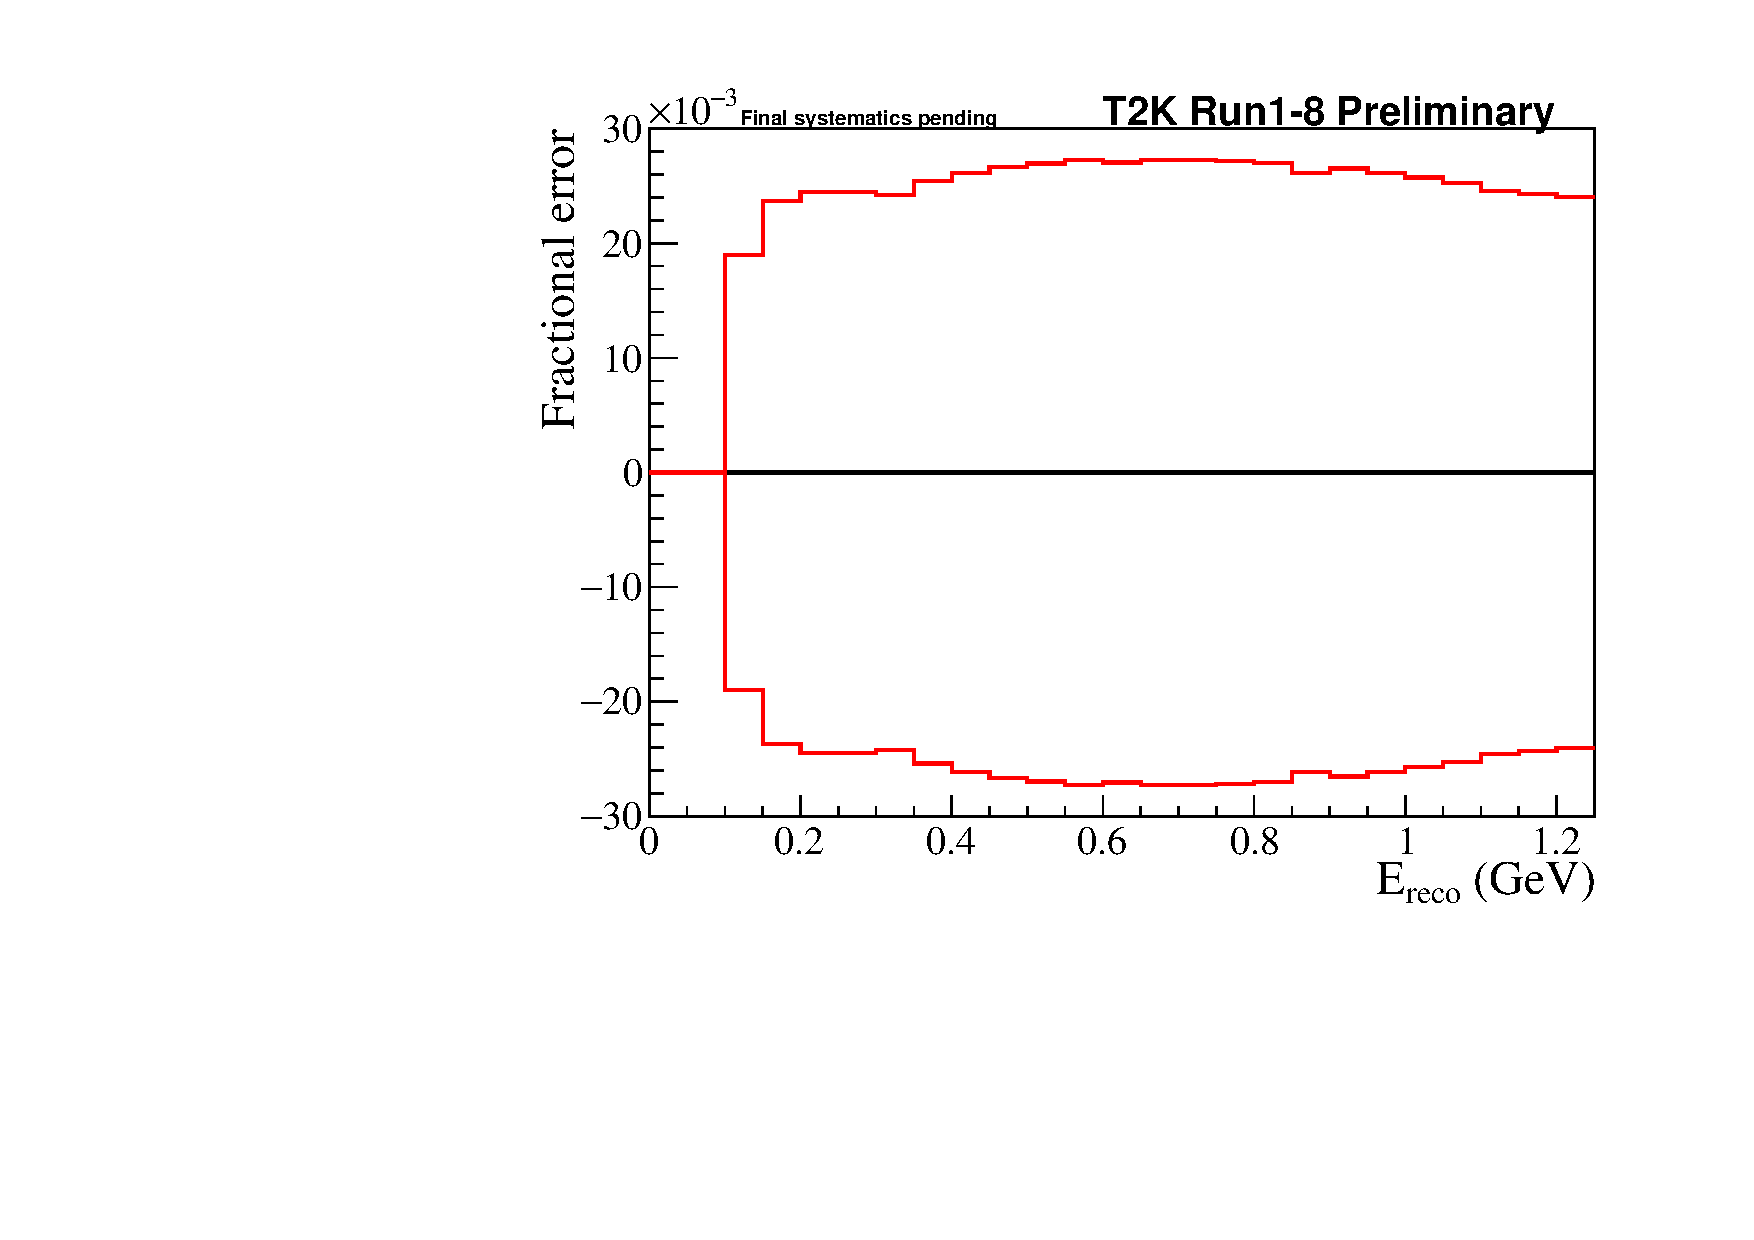
\includegraphics[width=0.9\textwidth]{systematics/envelopes/sk_errors/sk_error_table_1Re_xsec_nue_envelope_fractional}
		\caption{Electron-like, neutrino mode}
	\end{subfigure}
	\begin{subfigure}[b]{0.49\textwidth}
		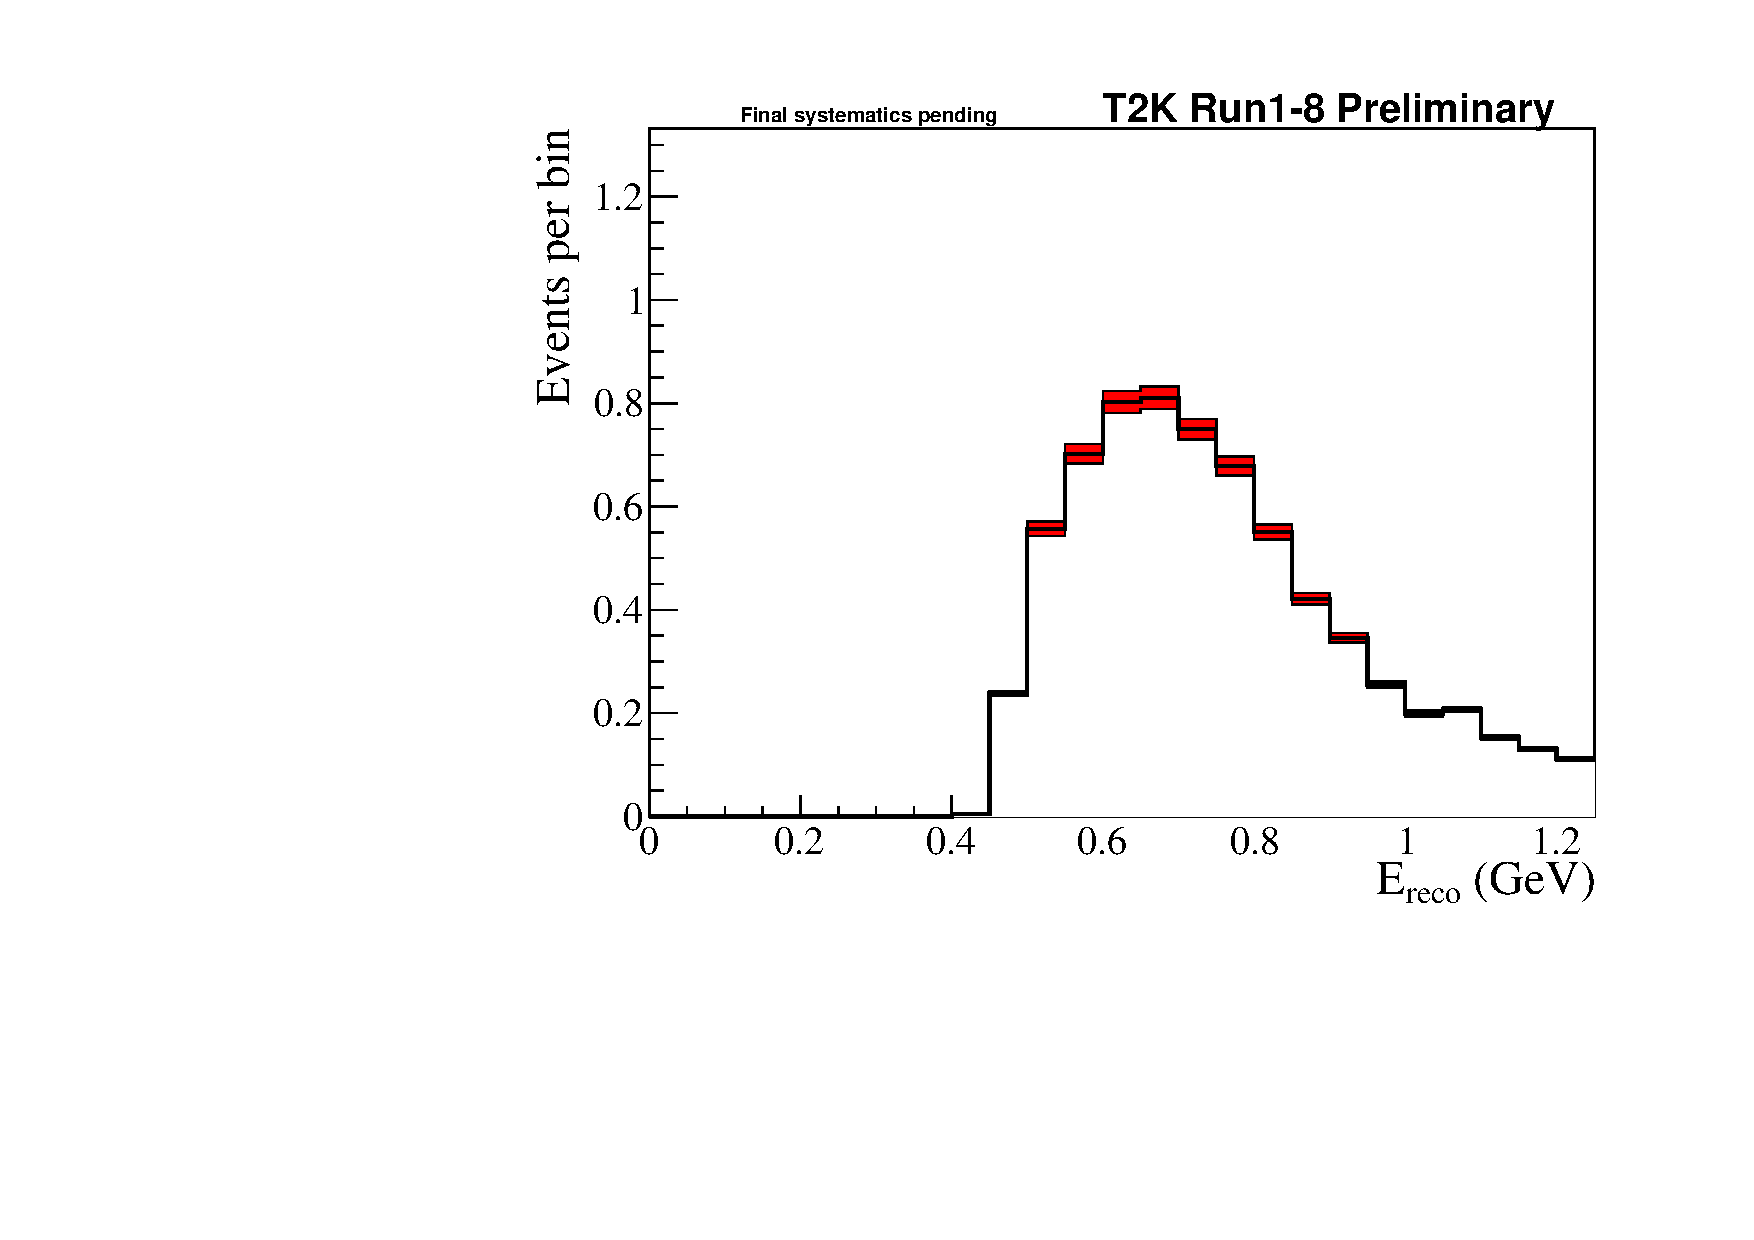
\includegraphics[width=0.9\textwidth]{systematics/envelopes/sk_errors/sk_error_table_MultiRe_xsec_nue_envelope}
		\caption{\nueCConepi-like, neutrino mode}
	\end{subfigure}
	\begin{subfigure}[b]{0.49\textwidth}
		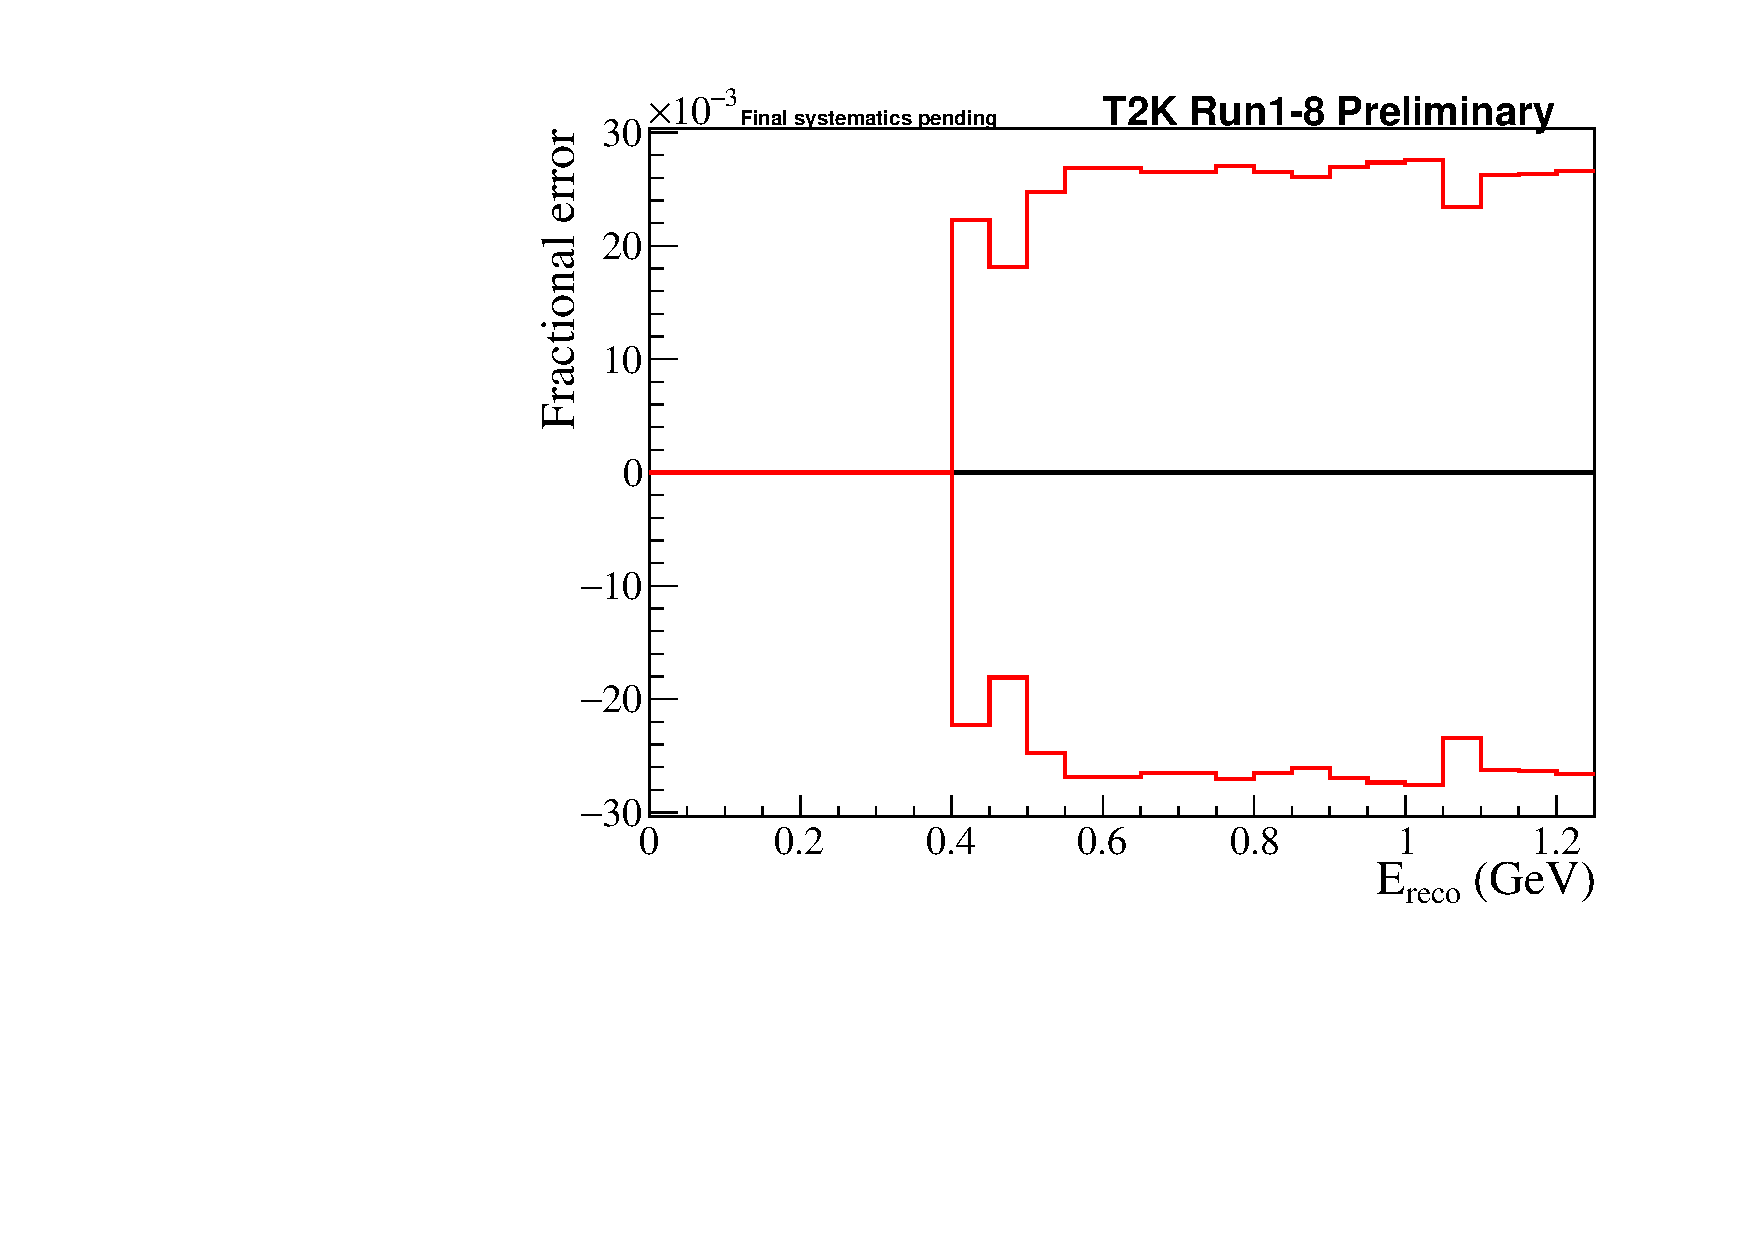
\includegraphics[width=0.9\textwidth]{systematics/envelopes/sk_errors/sk_error_table_MultiRe_xsec_nue_envelope_fractional}
		\caption{\nueCConepi-like, neutrino mode}
	\end{subfigure}
	\caption {
		Error envelopes (left) and fractional errors (right) for the reconstructed neutrino energy spectrum for the unconstrained electron neutrino cross-section systematic parameters. \num{1e4} toys are generated for the Asimov data set A with randomized systematic parameters with correlations taken into account.
	}
	\label{fig:sk_envelopes_xsec_nue}
\end{figure*}
\clearpage

\begin{figure*}
	\center
	\begin{subfigure}[b]{0.49\textwidth}
		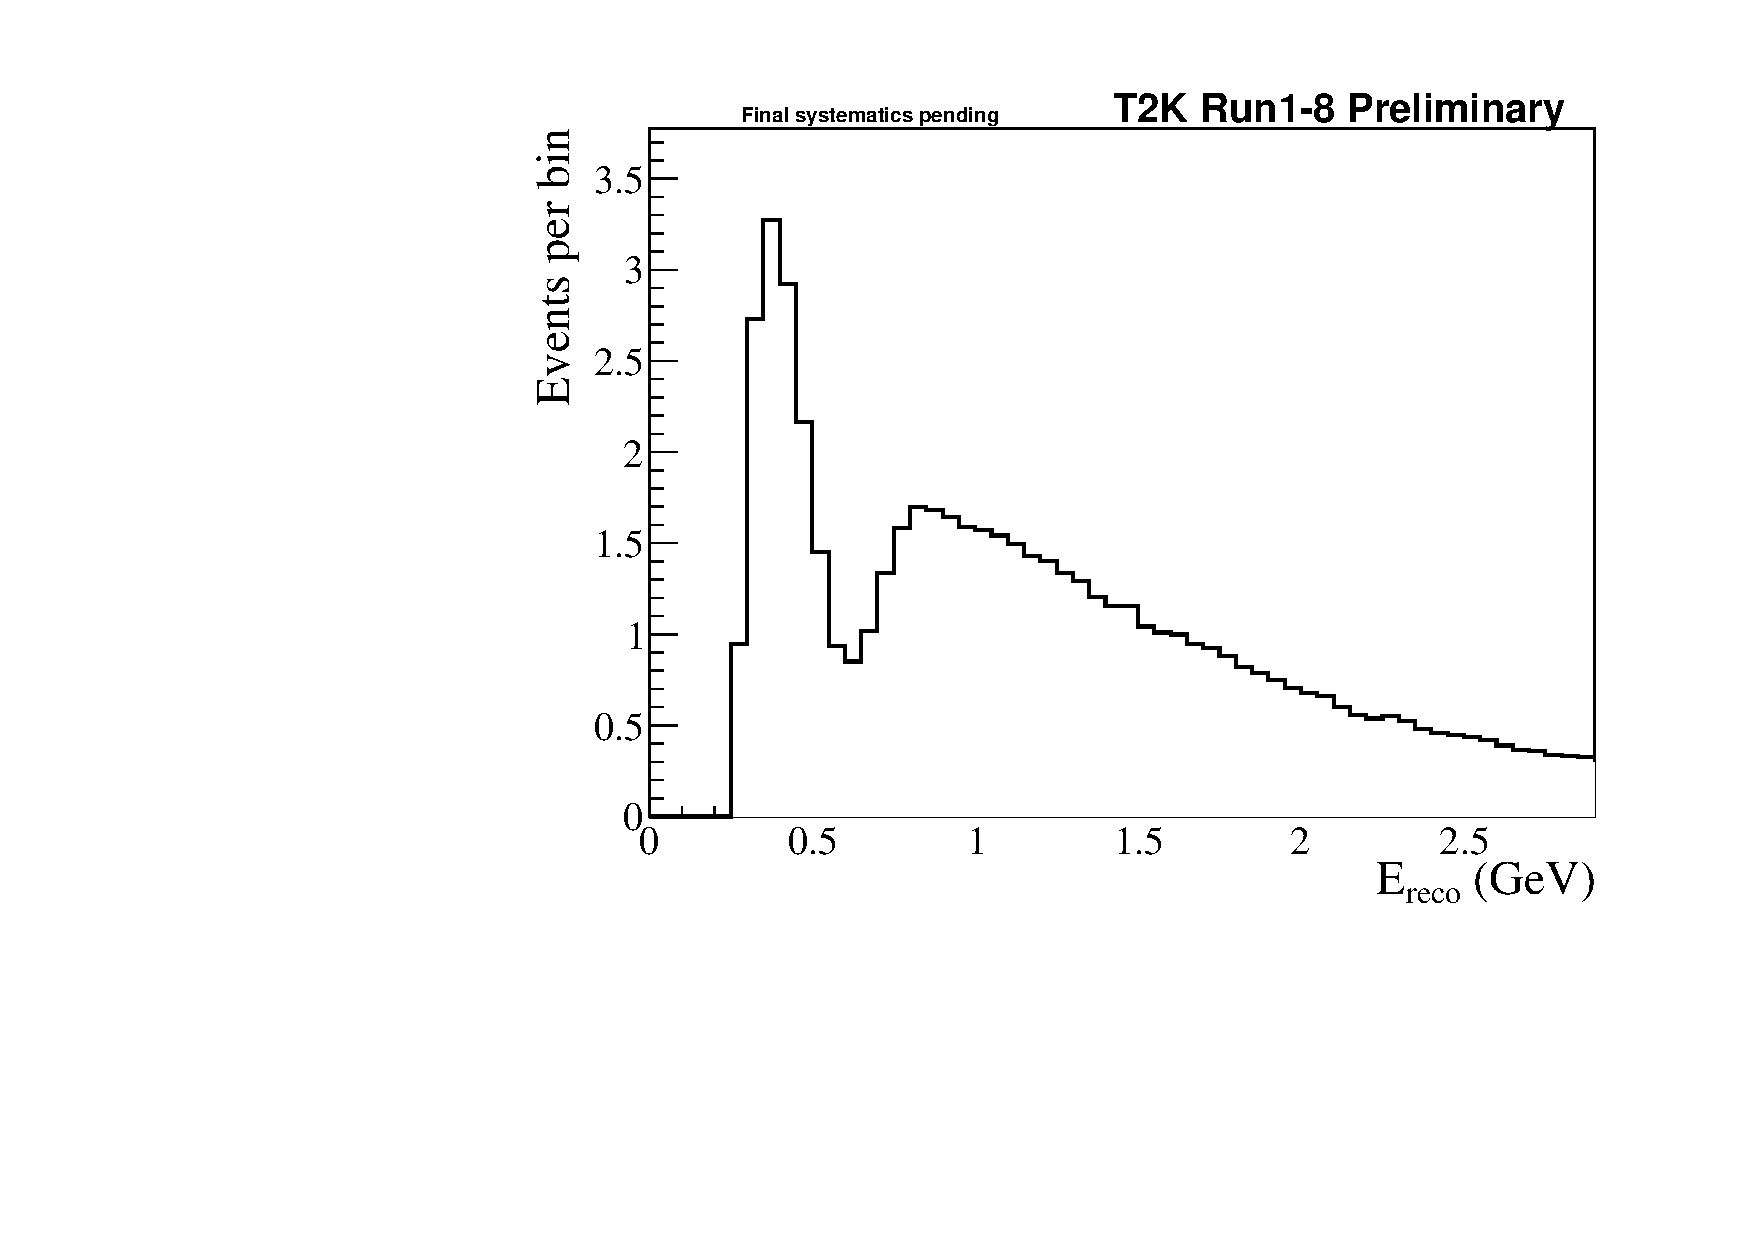
\includegraphics[width=0.9\textwidth]{systematics/envelopes/sk_errors/sk_error_table_RHC1Rmu_xsec_nue_envelope}
		\caption{Muon-like, antineutrino mode}
	\end{subfigure}
	\begin{subfigure}[b]{0.49\textwidth}
		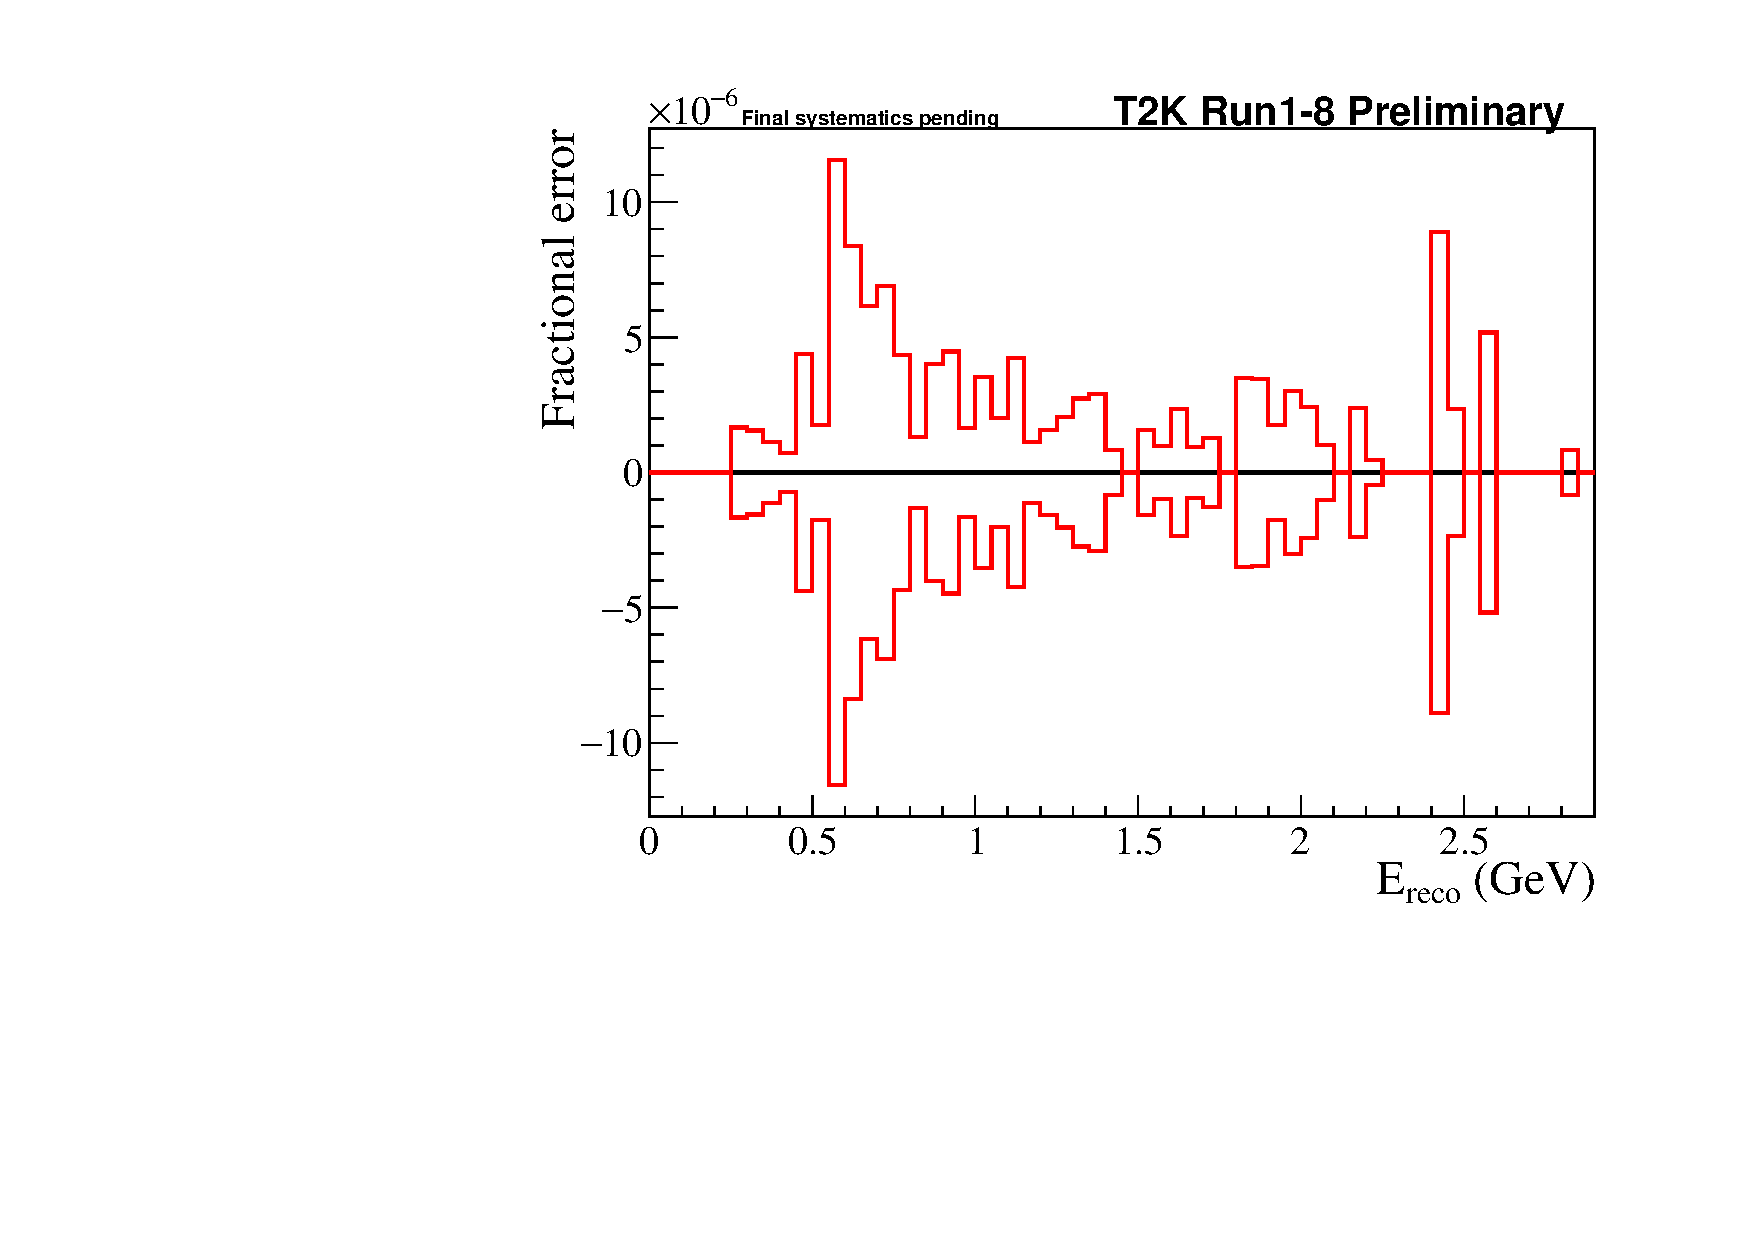
\includegraphics[width=0.9\textwidth]{systematics/envelopes/sk_errors/sk_error_table_RHC1Rmu_xsec_nue_envelope_fractional}
		\caption{Muon-like, antineutrino mode}
	\end{subfigure}
	\begin{subfigure}[b]{0.49\textwidth}
		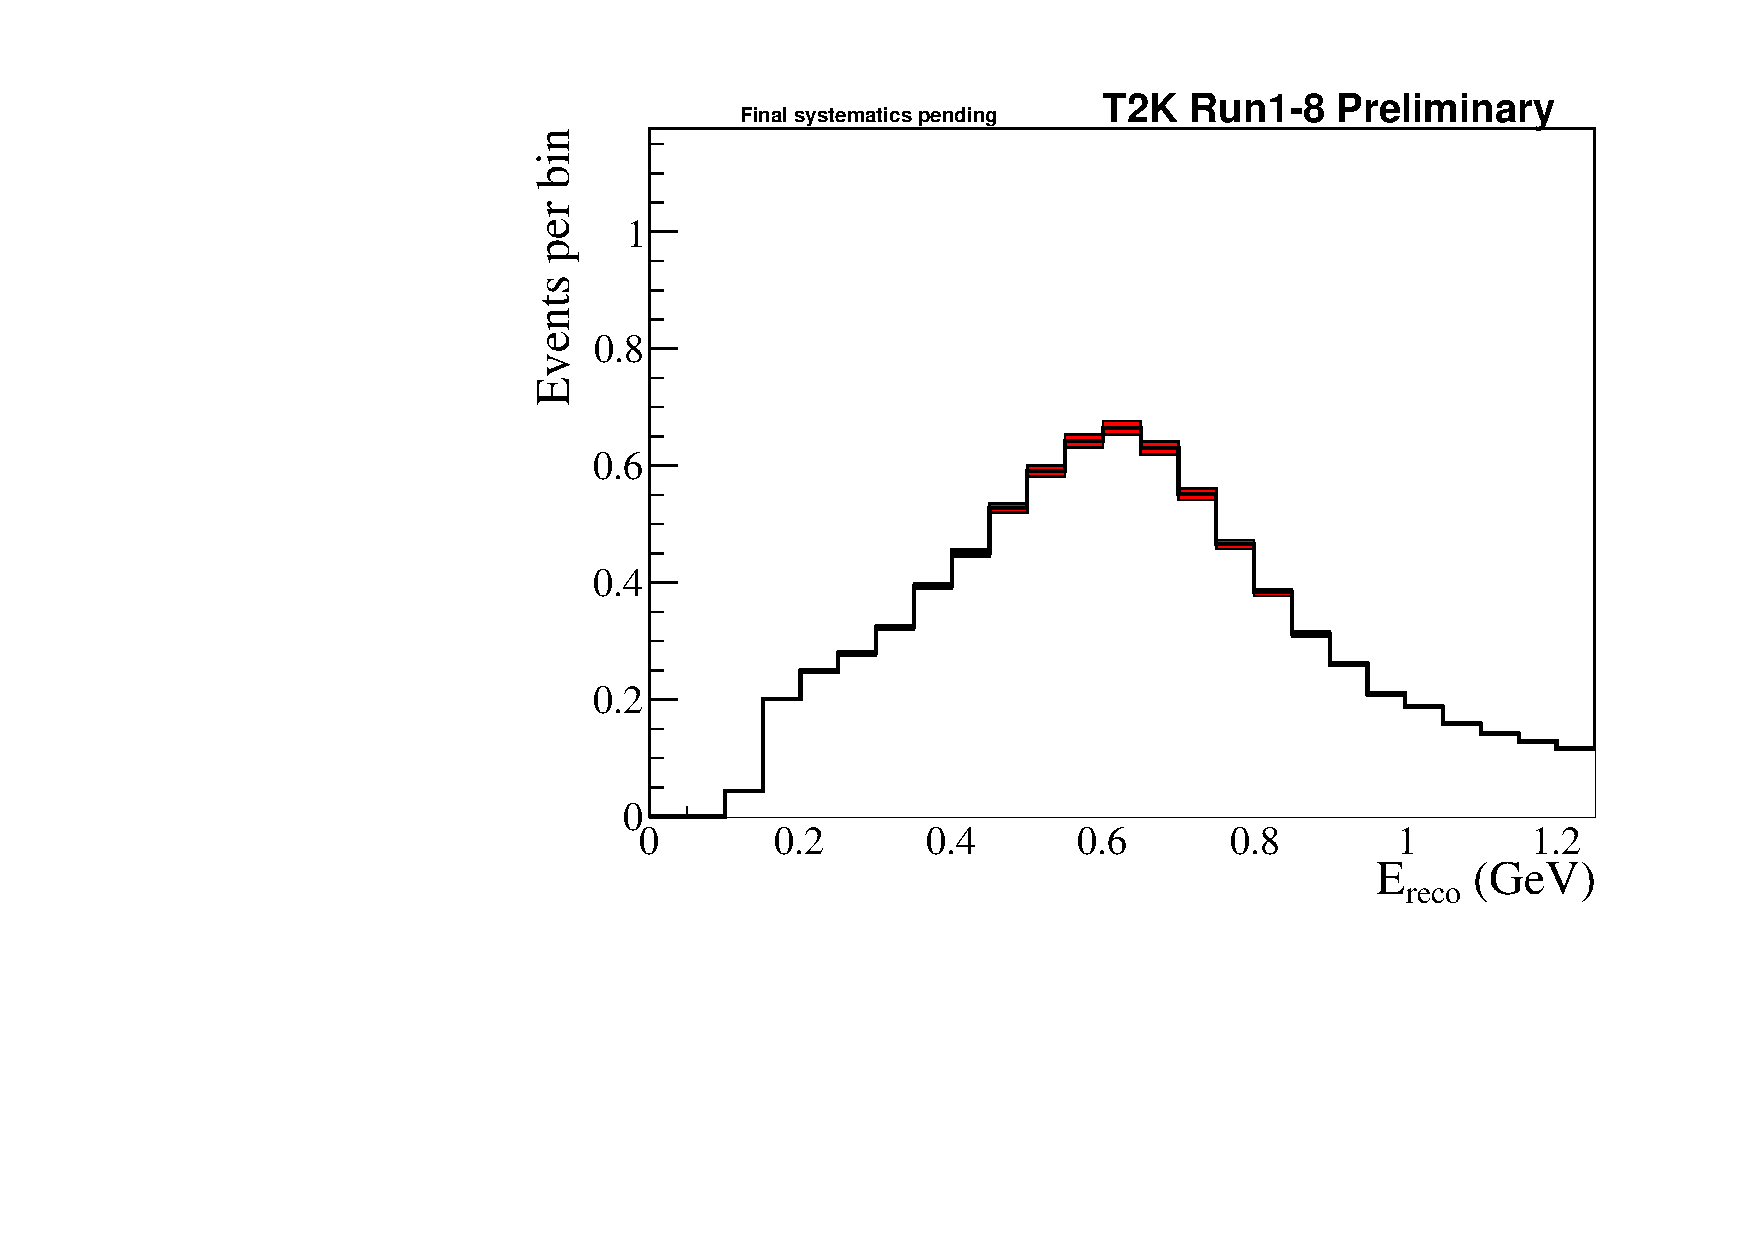
\includegraphics[width=0.9\textwidth]{systematics/envelopes/sk_errors/sk_error_table_RHC1Re_xsec_nue_envelope}
		\caption{Electron-like antineutrino mode}
	\end{subfigure}
	\begin{subfigure}[b]{0.49\textwidth}
		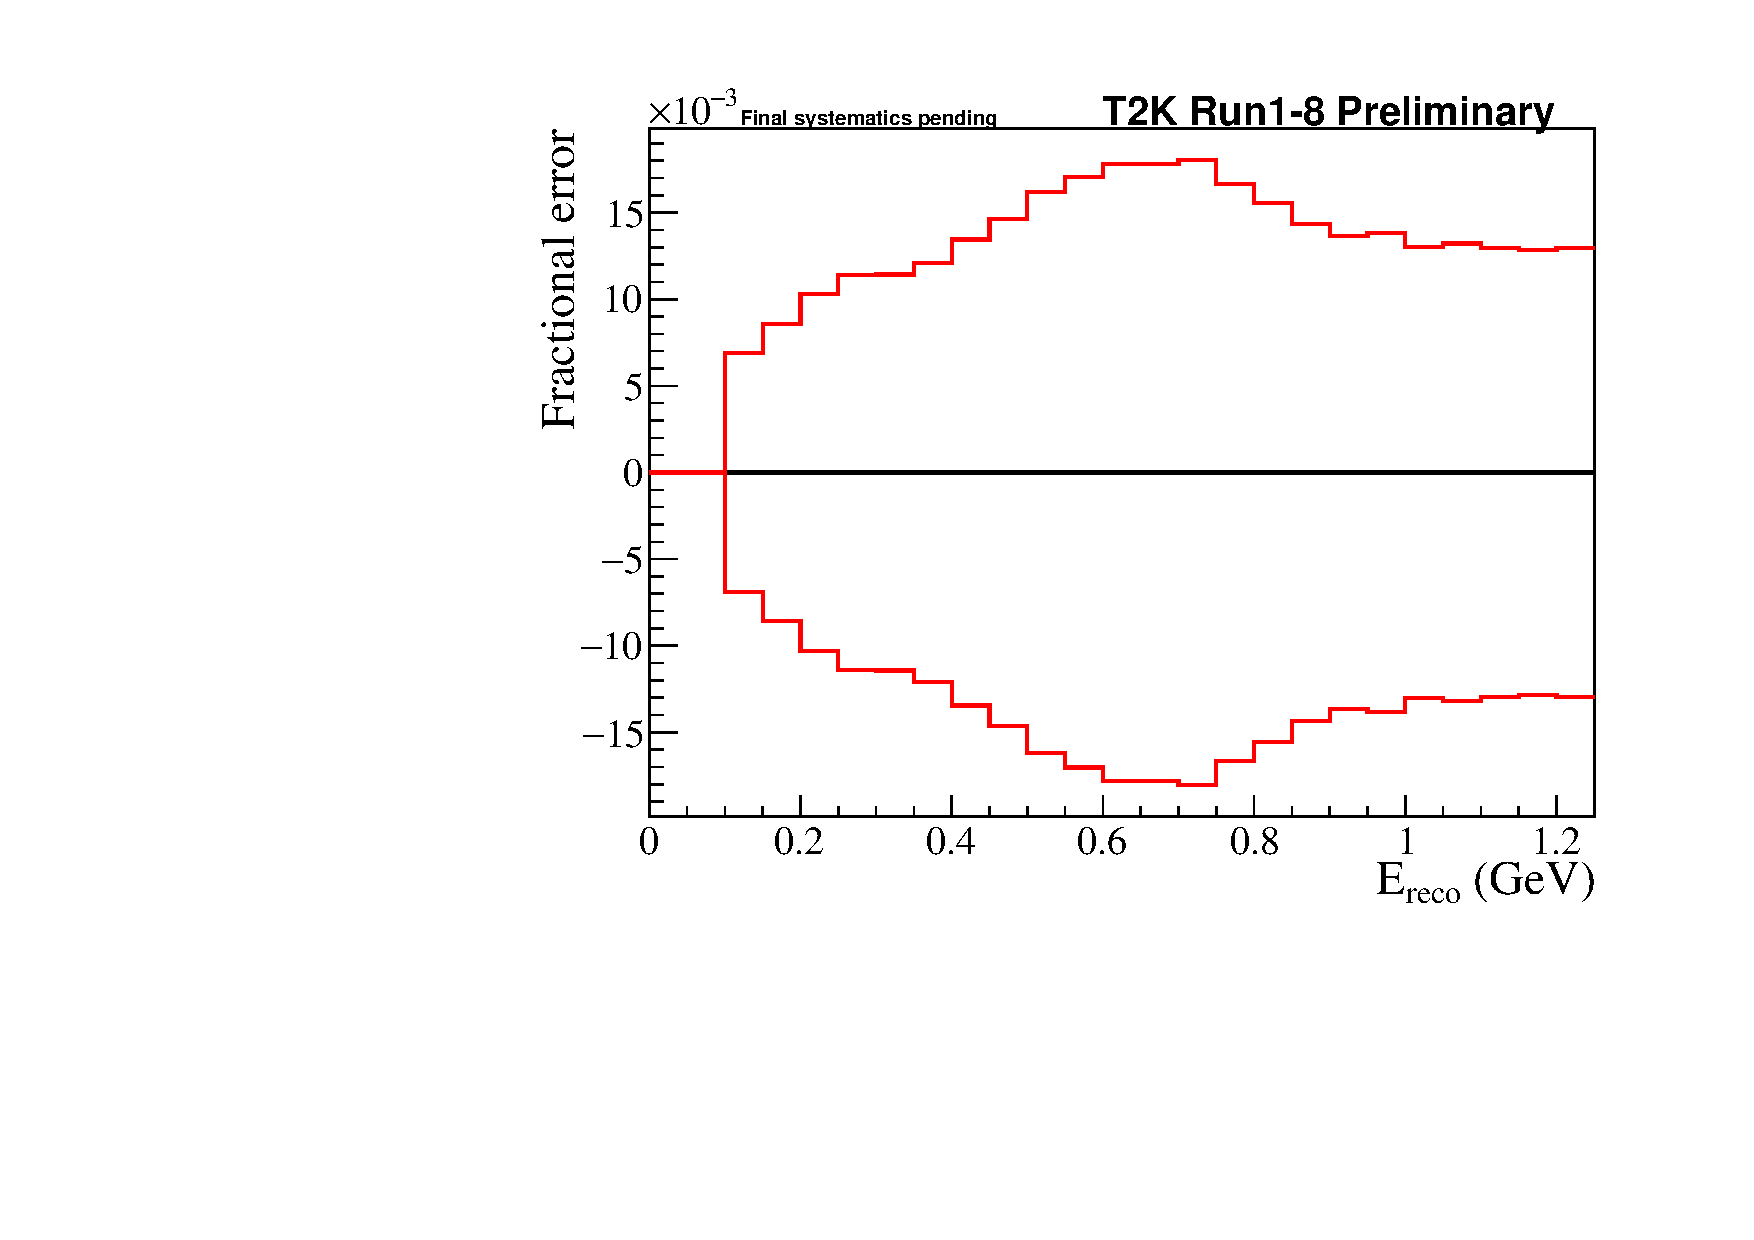
\includegraphics[width=0.9\textwidth]{systematics/envelopes/sk_errors/sk_error_table_RHC1Re_xsec_nue_envelope_fractional}
		\caption{Electron-like antineutrino mode}
	\end{subfigure}
	\caption {
		Error envelopes (left) and fractional errors (right) for the reconstructed neutrino energy spectrum for the unconstrained electron neutrino cross-section systematic parameters. \num{1e4} toys are generated for the Asimov data set A with randomized systematic parameters with correlations taken into account.
	}
	\label{fig:sk_envelopes_xsec_nue_b}
\end{figure*}
\clearpage
\begin{figure*}
	\center
	\begin{subfigure}[b]{0.49\textwidth}
		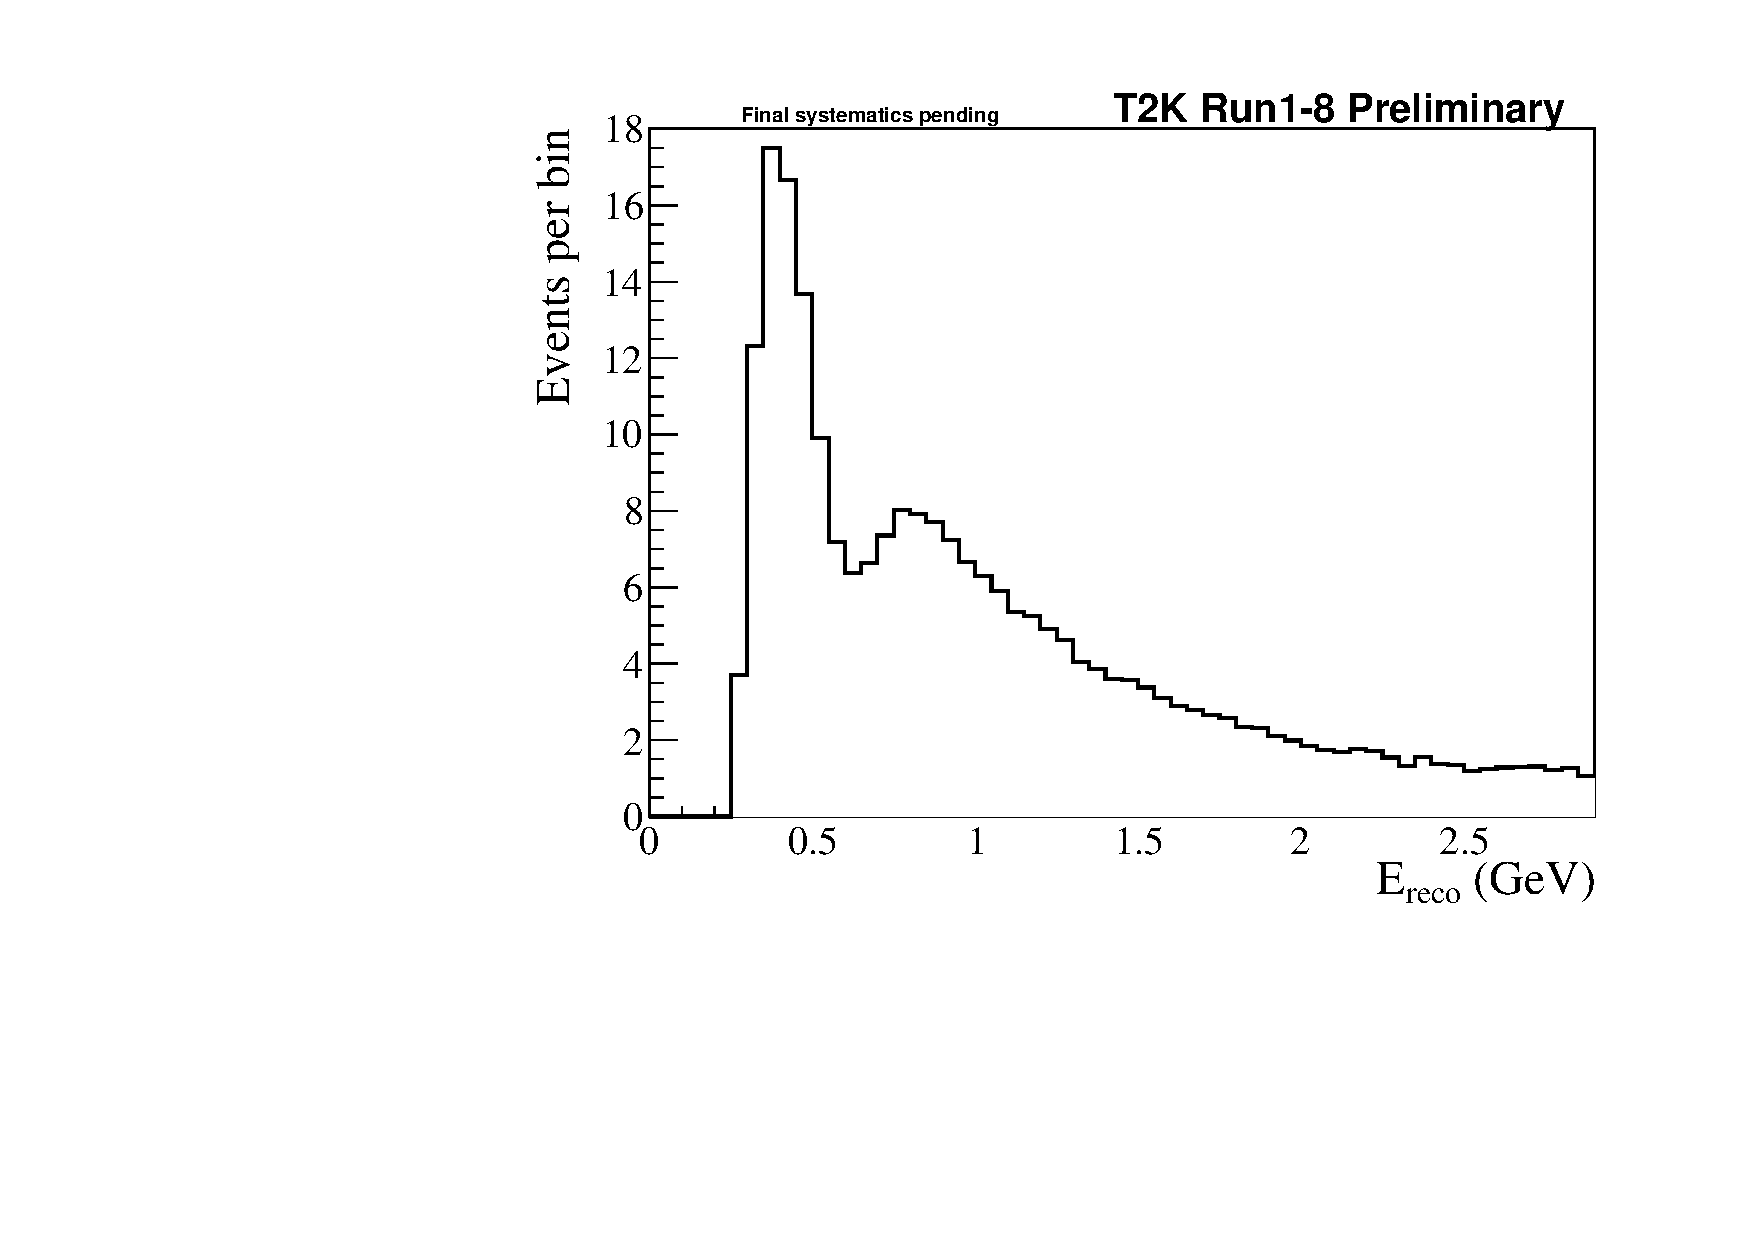
\includegraphics[width=0.9\textwidth]{systematics/envelopes/sk_errors/sk_error_table_1Rmu_xsec_ncgamma_envelope}
		\caption{Muon-like, neutrino mode}
	\end{subfigure}
	\begin{subfigure}[b]{0.49\textwidth}
		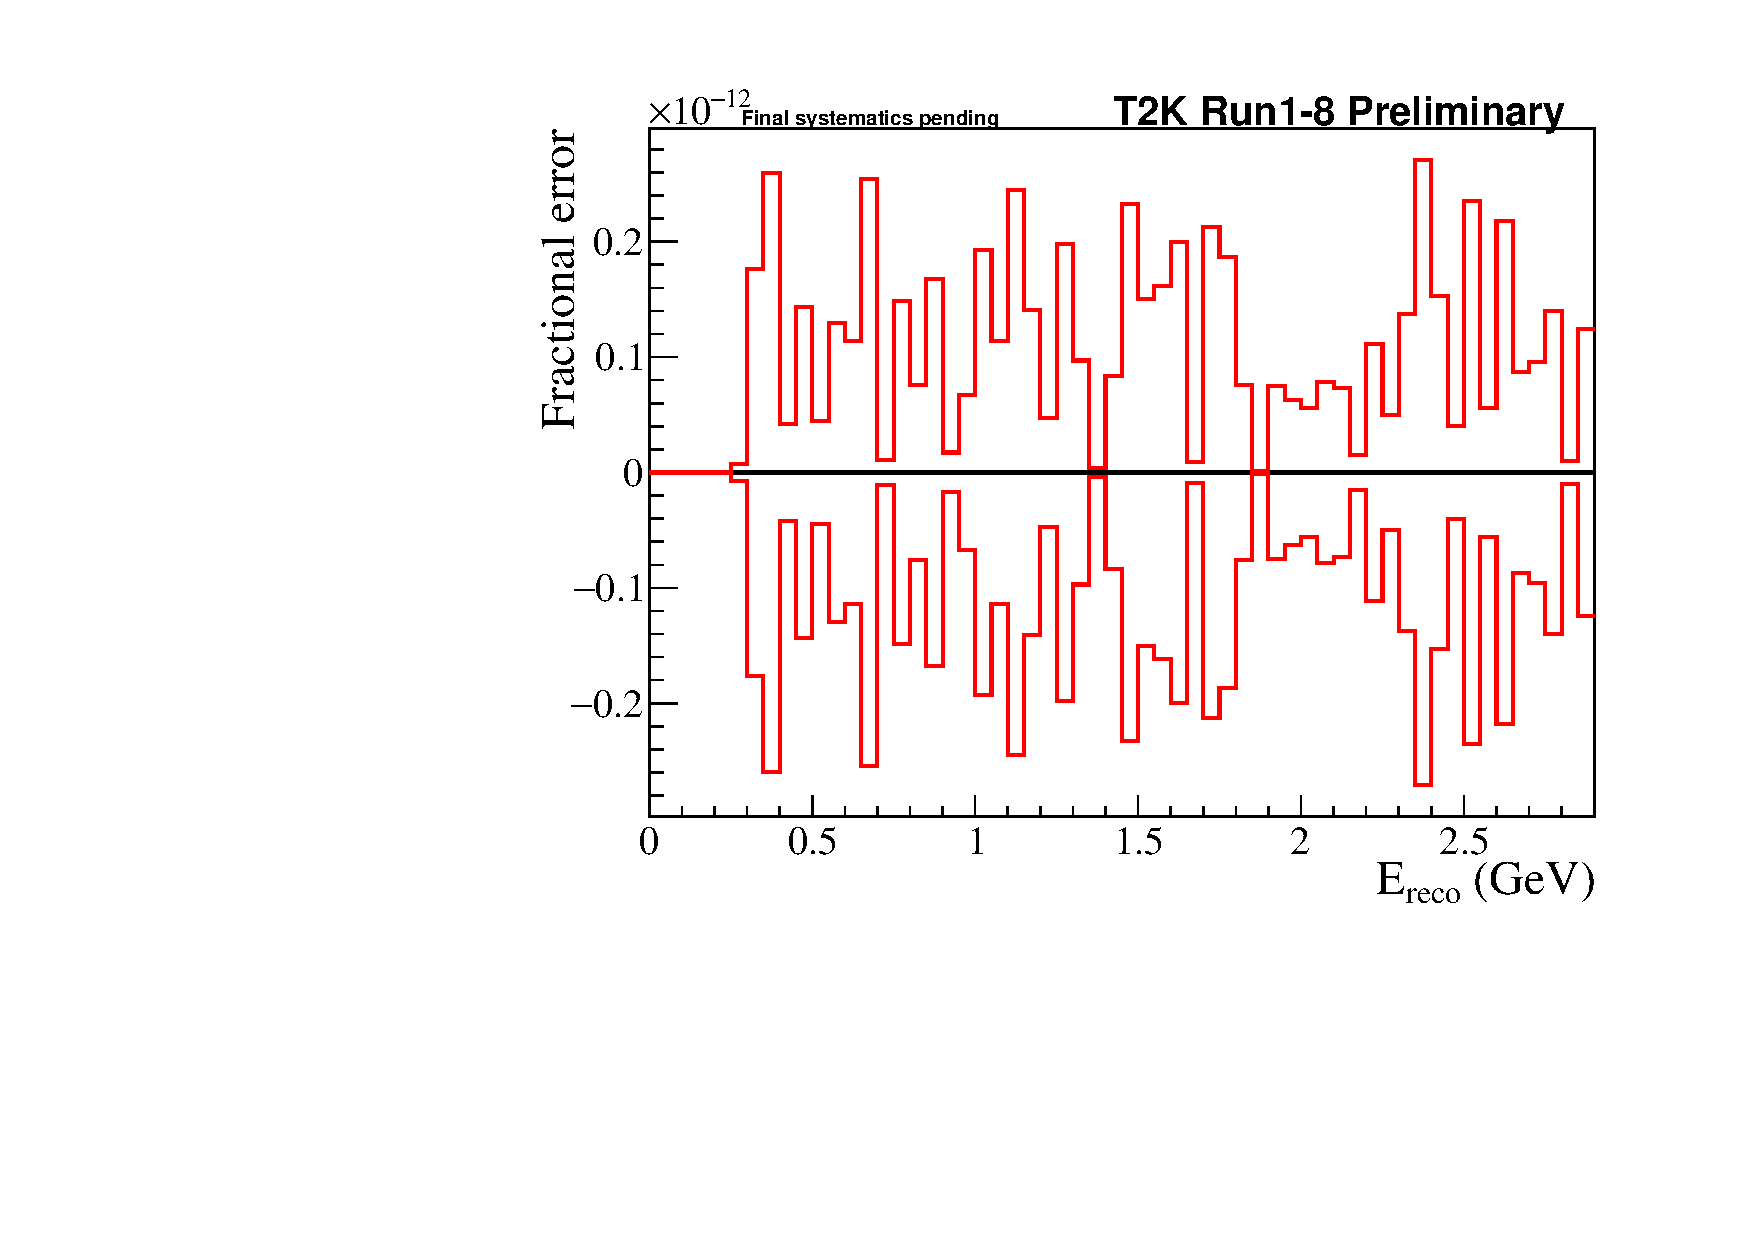
\includegraphics[width=0.9\textwidth]{systematics/envelopes/sk_errors/sk_error_table_1Rmu_xsec_ncgamma_envelope_fractional}
		\caption{Muon-like, neutrino mode}
	\end{subfigure}
	\begin{subfigure}[b]{0.49\textwidth}
		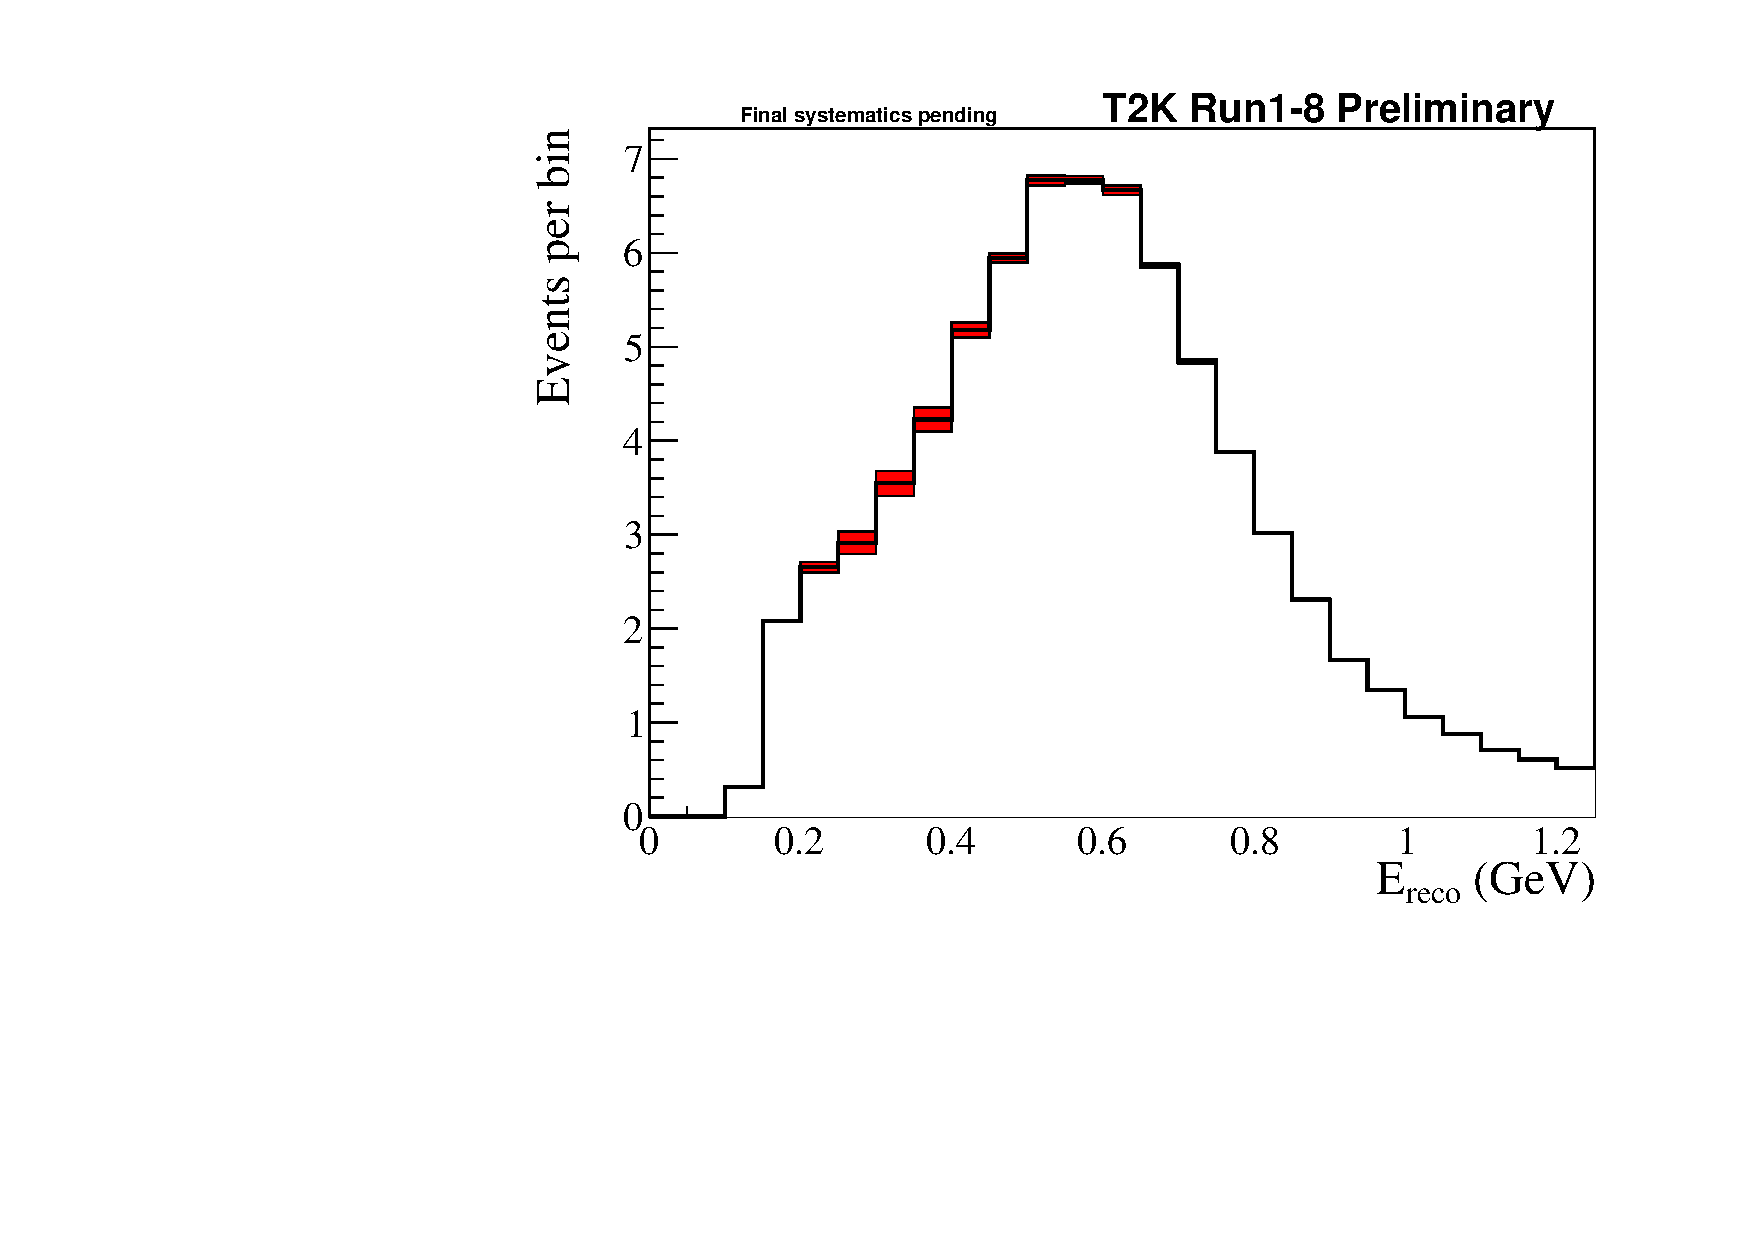
\includegraphics[width=0.9\textwidth]{systematics/envelopes/sk_errors/sk_error_table_1Re_xsec_ncgamma_envelope}
		\caption{Electron-like, neutrino mode}
	\end{subfigure}
	\begin{subfigure}[b]{0.49\textwidth}
		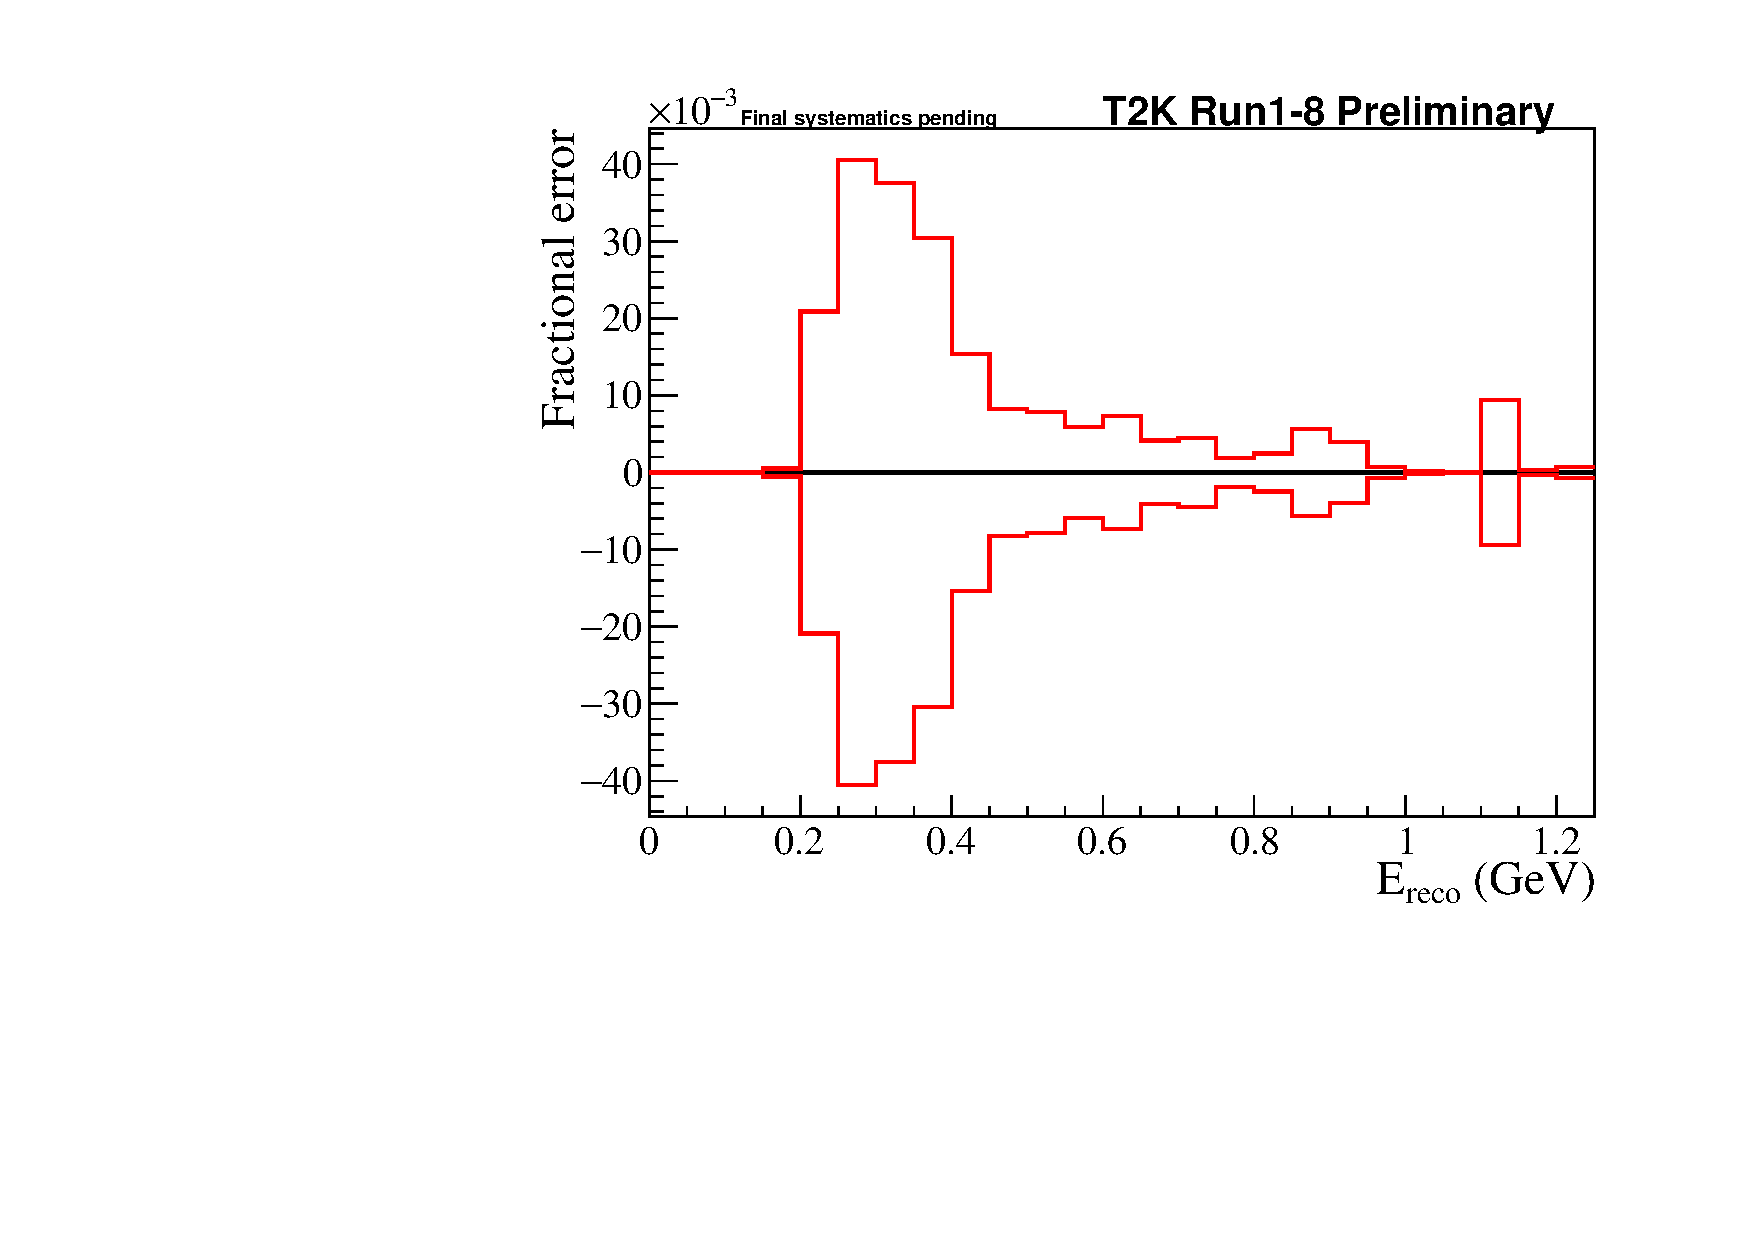
\includegraphics[width=0.9\textwidth]{systematics/envelopes/sk_errors/sk_error_table_1Re_xsec_ncgamma_envelope_fractional}
		\caption{Electron-like, neutrino mode}
	\end{subfigure}
	\begin{subfigure}[b]{0.49\textwidth}
		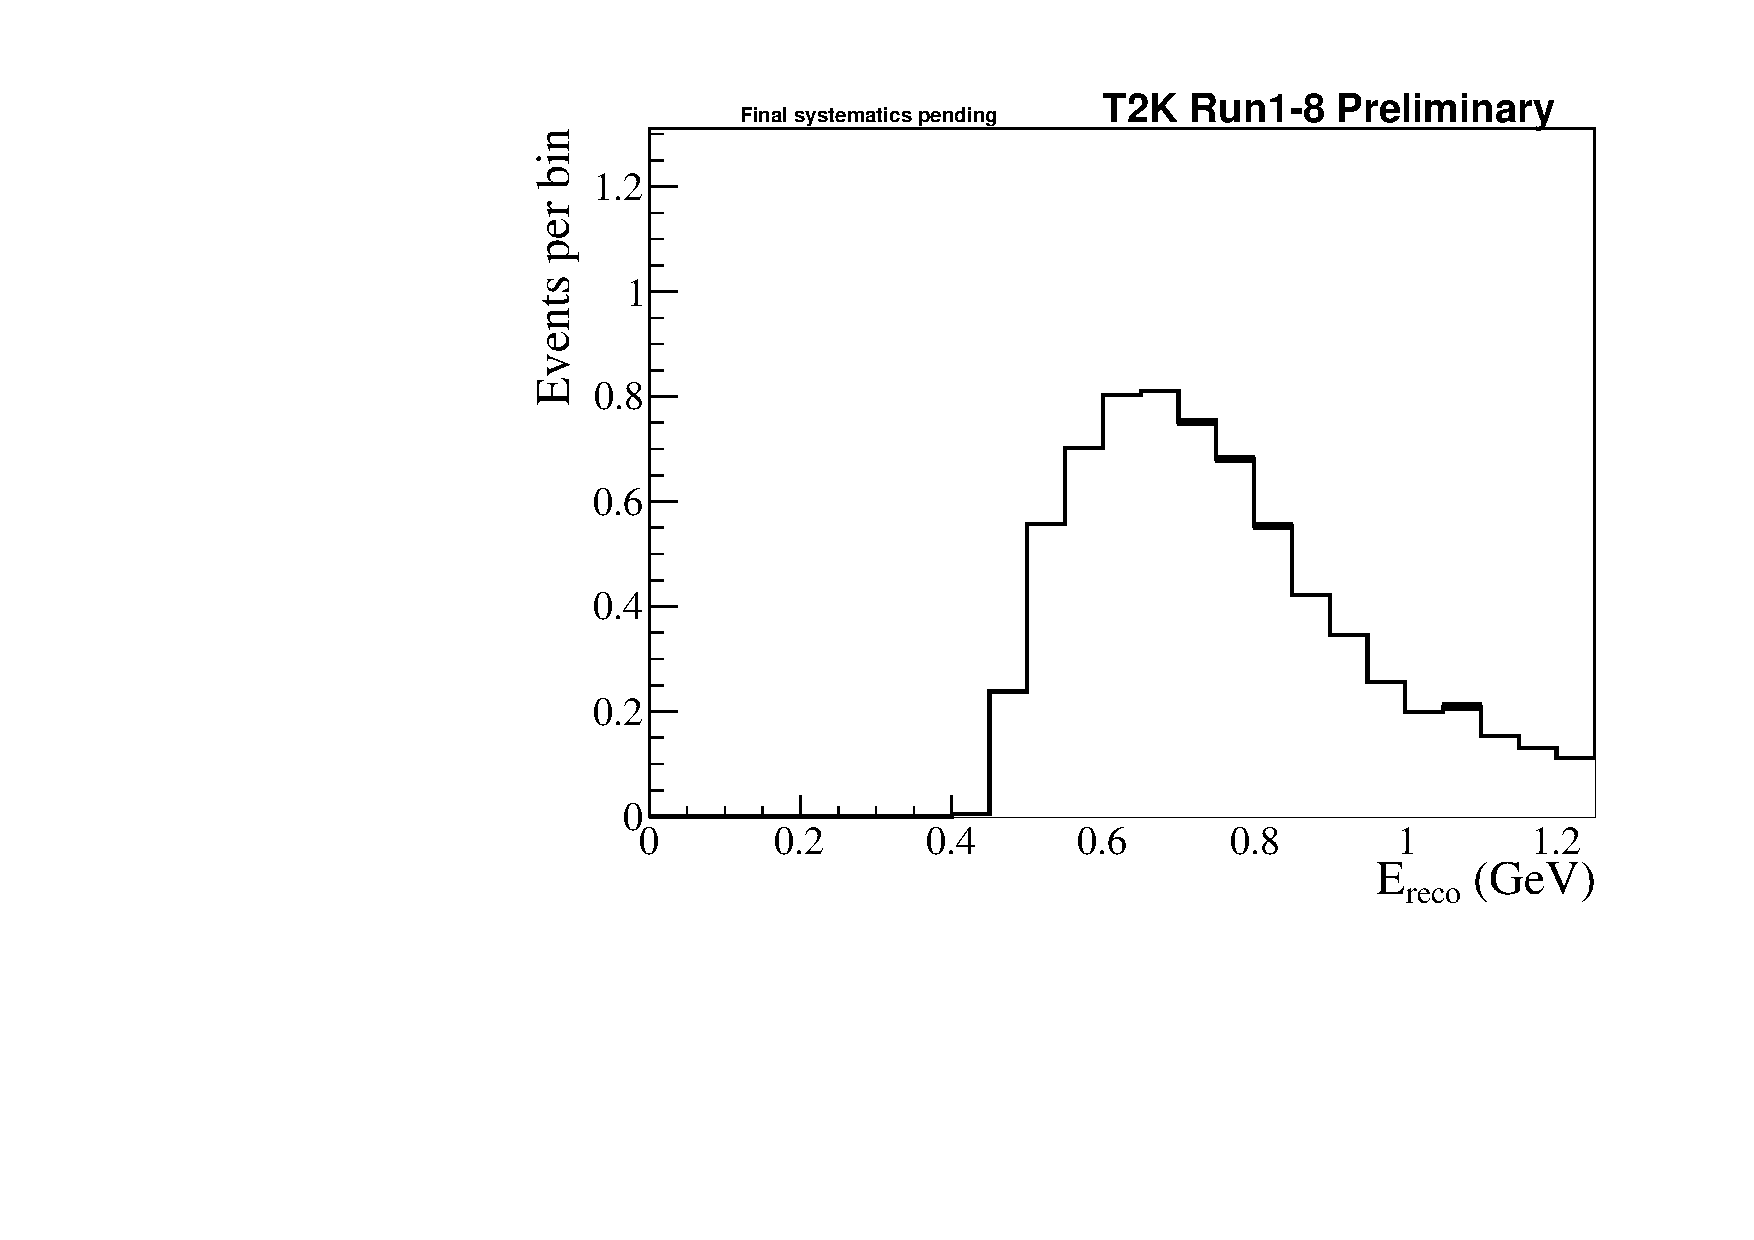
\includegraphics[width=0.9\textwidth]{systematics/envelopes/sk_errors/sk_error_table_MultiRe_xsec_ncgamma_envelope}
		\caption{\nueCConepi-like, neutrino mode}
	\end{subfigure}
	\begin{subfigure}[b]{0.49\textwidth}
		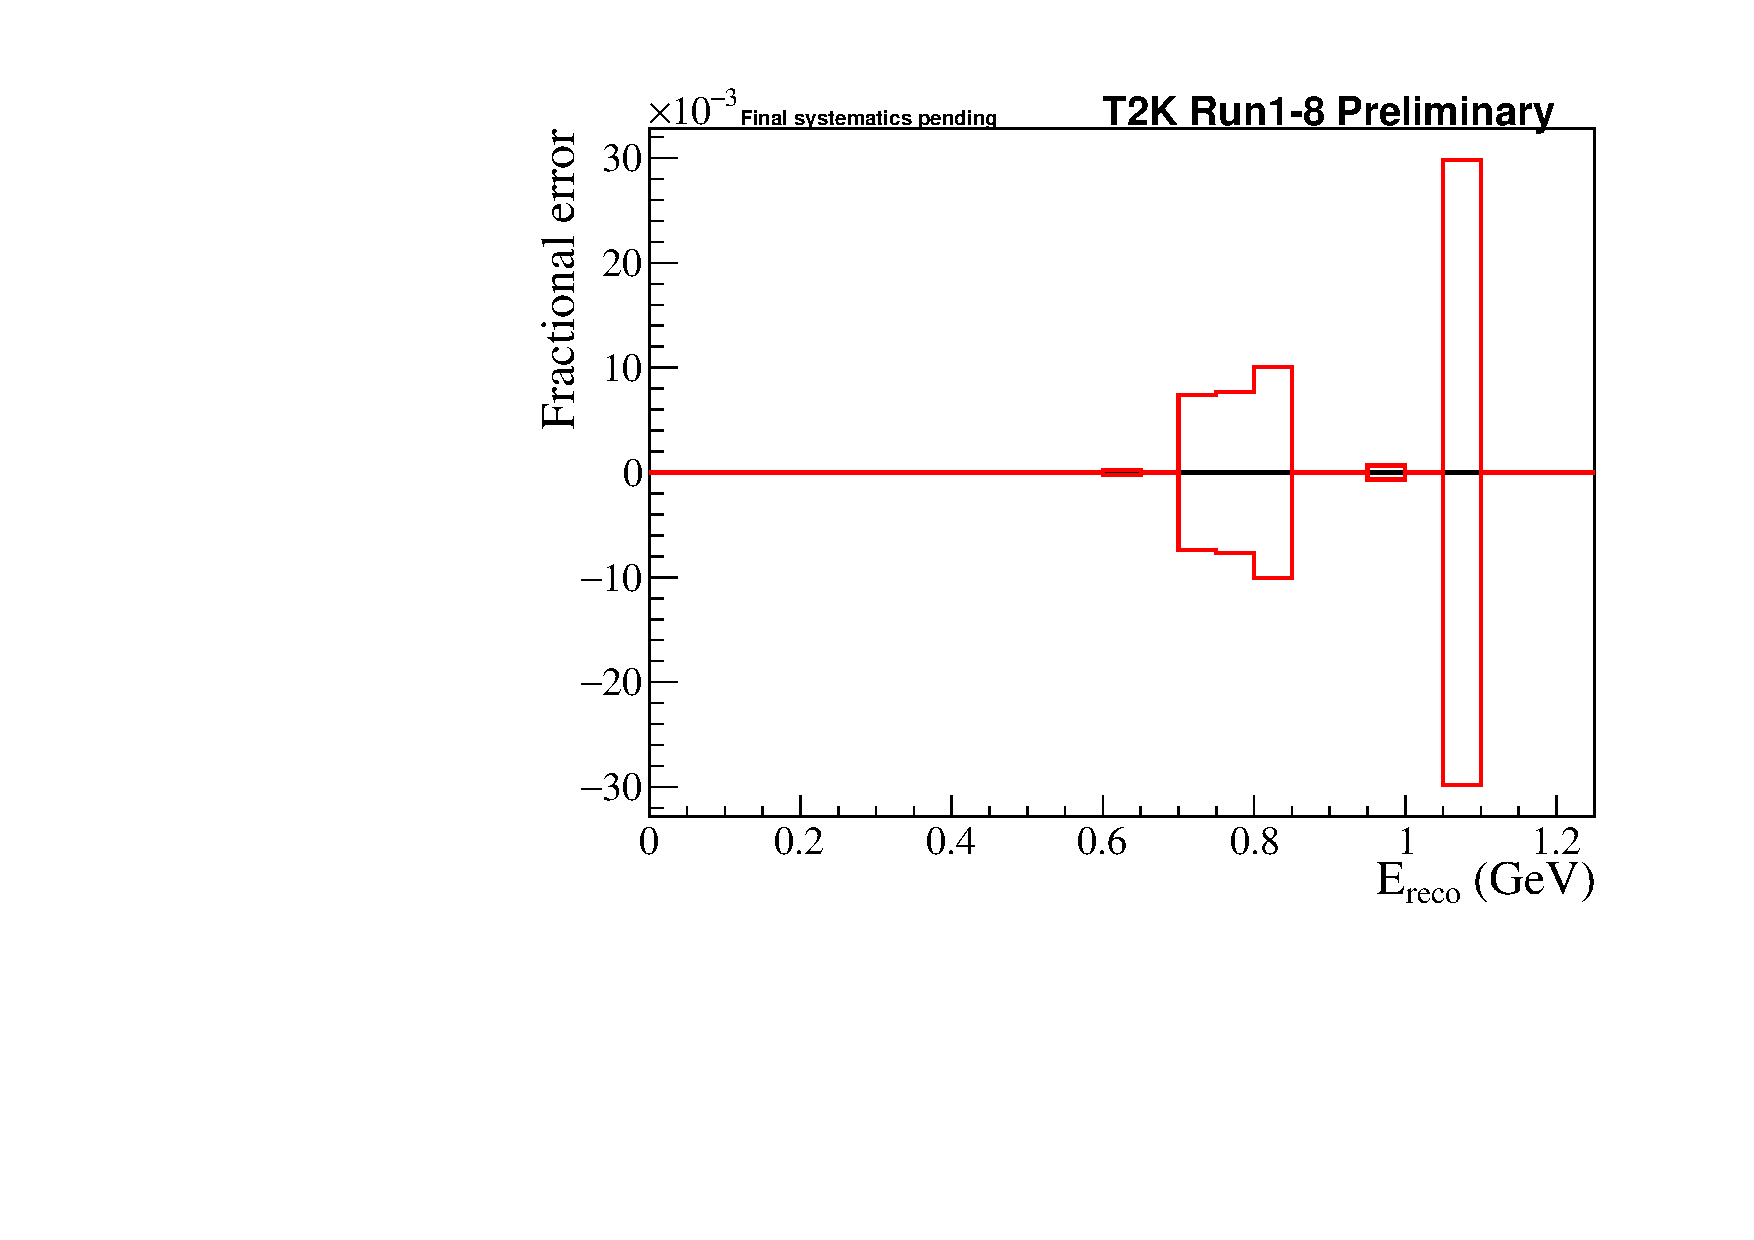
\includegraphics[width=0.9\textwidth]{systematics/envelopes/sk_errors/sk_error_table_MultiRe_xsec_ncgamma_envelope_fractional}
		\caption{\nueCConepi-like, neutrino mode}
	\end{subfigure}
	\caption {
		Error envelopes (left) and fractional error (right) for the reconstructed neutrino energy spectrum for the unconstrained NC$1\gamma$ systematic parameters. \num{1e4} toys are generated for the Asimov data set A with randomized systematic parameters with correlations taken into account.
	}
	\label{fig:sk_envelopes_xsec_ncgamma}
\end{figure*}
\clearpage

\begin{figure*}
	\center
	\begin{subfigure}[b]{0.49\textwidth}
		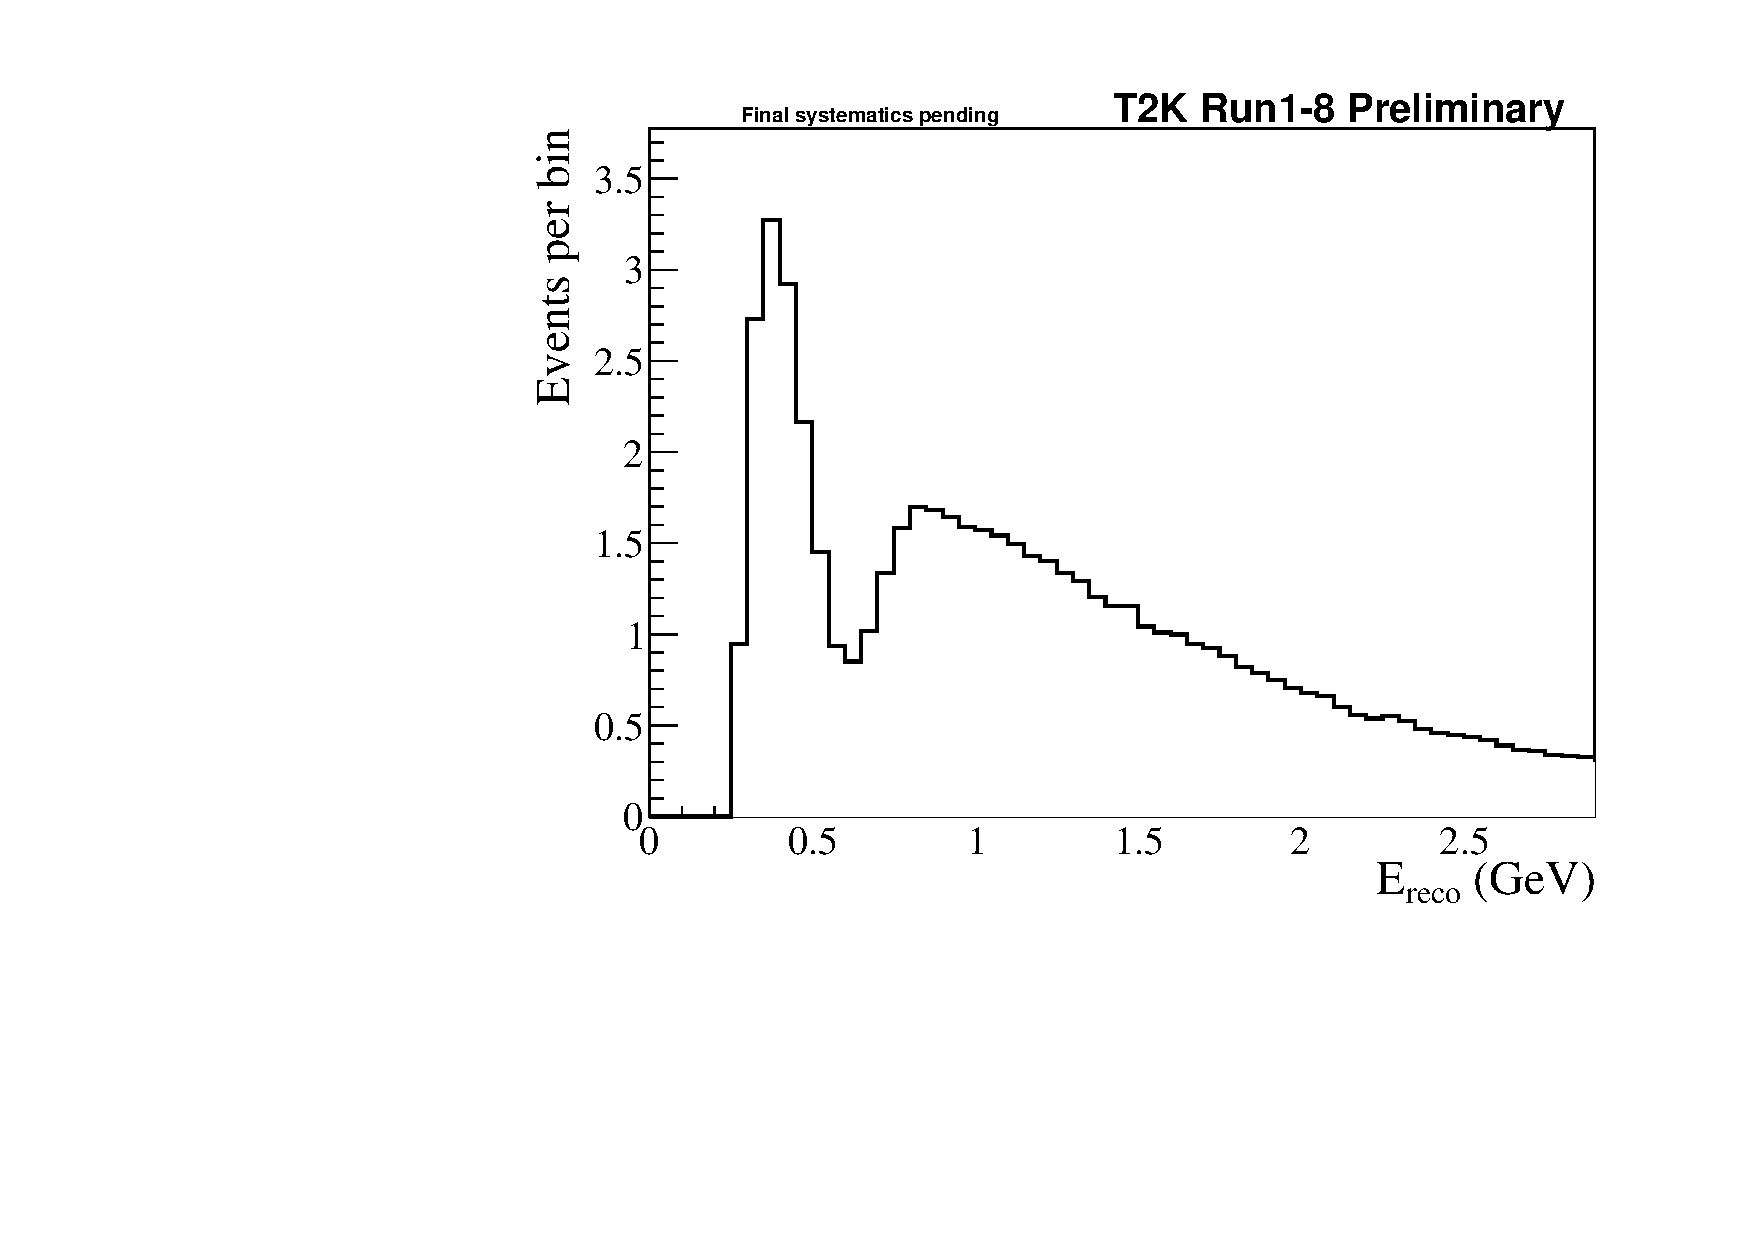
\includegraphics[width=0.9\textwidth]{systematics/envelopes/sk_errors/sk_error_table_RHC1Rmu_xsec_ncgamma_envelope}
		\caption{Muon-like, antineutrino mode}
	\end{subfigure}
	\begin{subfigure}[b]{0.49\textwidth}
		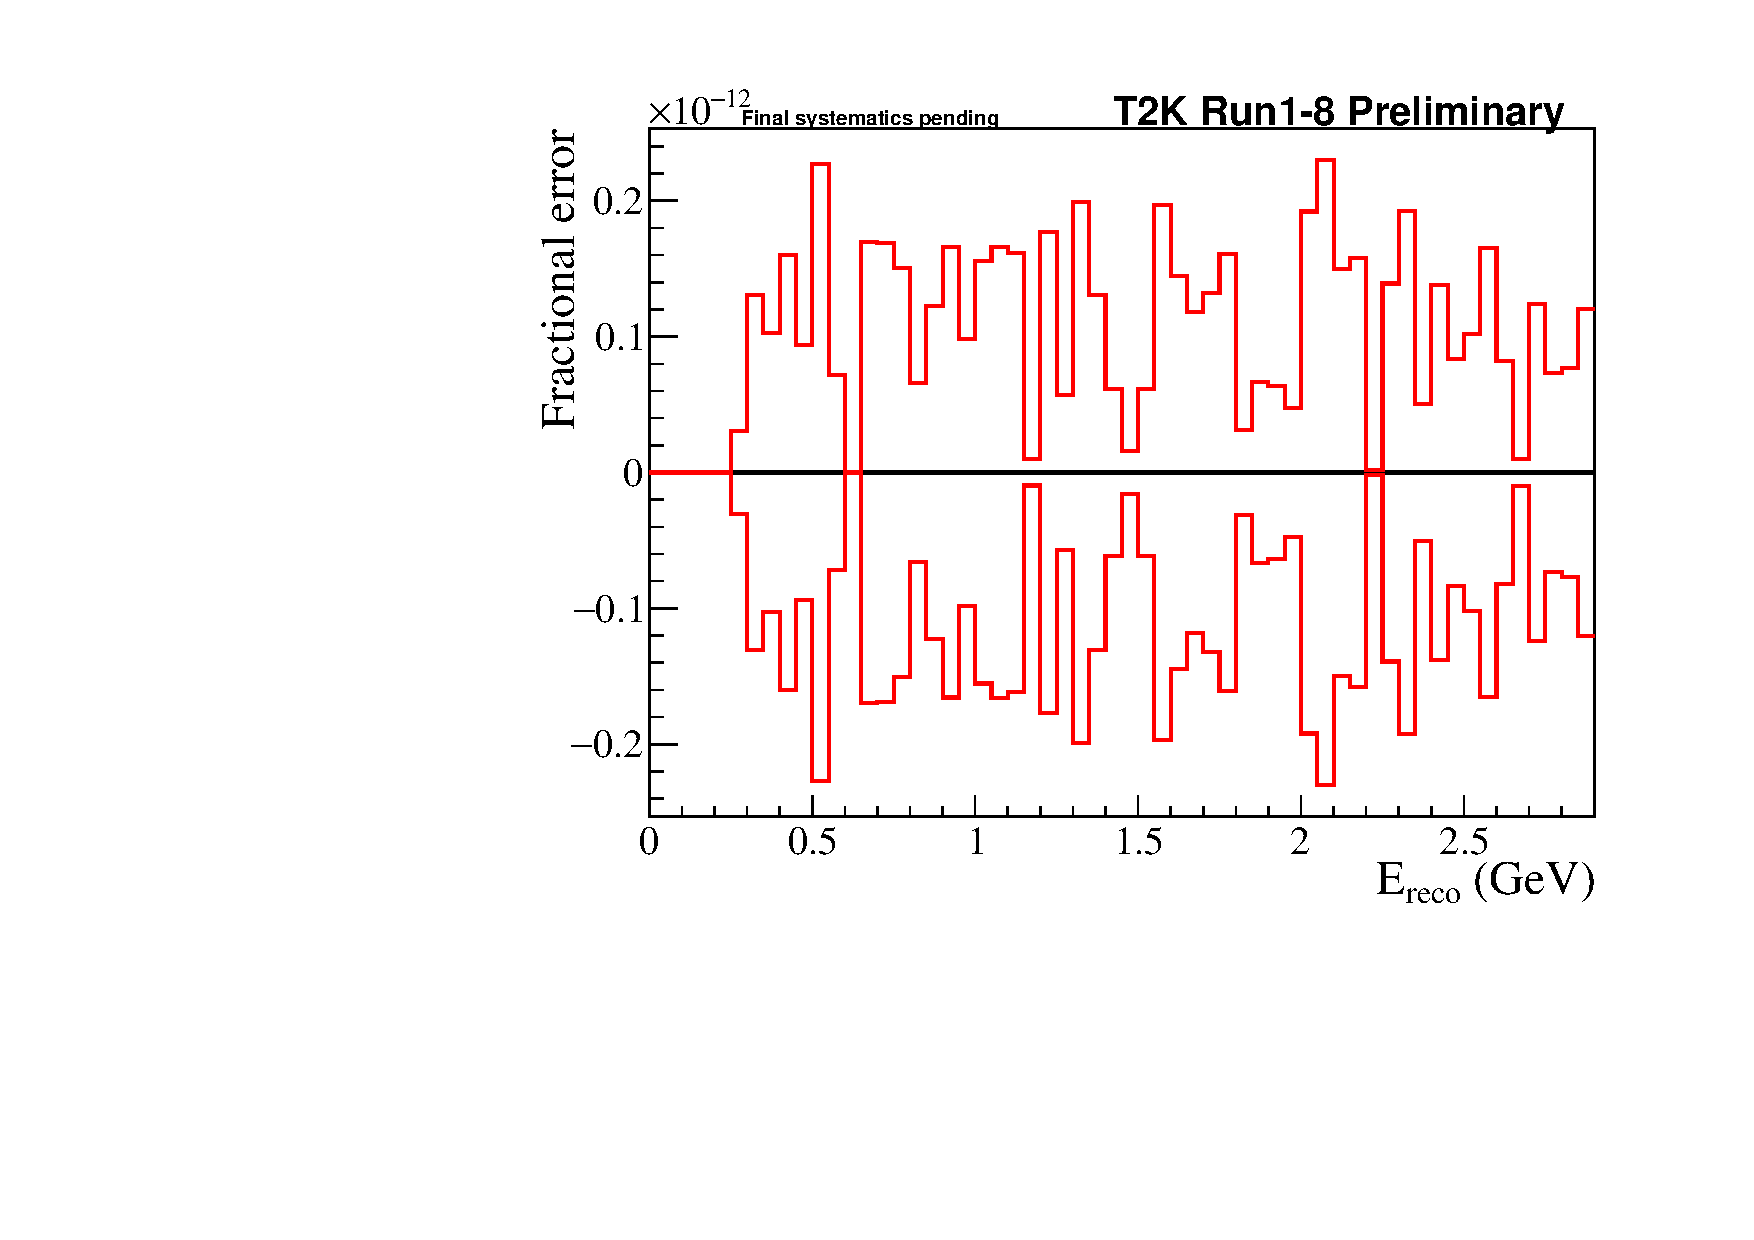
\includegraphics[width=0.9\textwidth]{systematics/envelopes/sk_errors/sk_error_table_RHC1Rmu_xsec_ncgamma_envelope_fractional}
		\caption{Muon-like, antineutrino mode}
	\end{subfigure}
	\begin{subfigure}[b]{0.49\textwidth}
		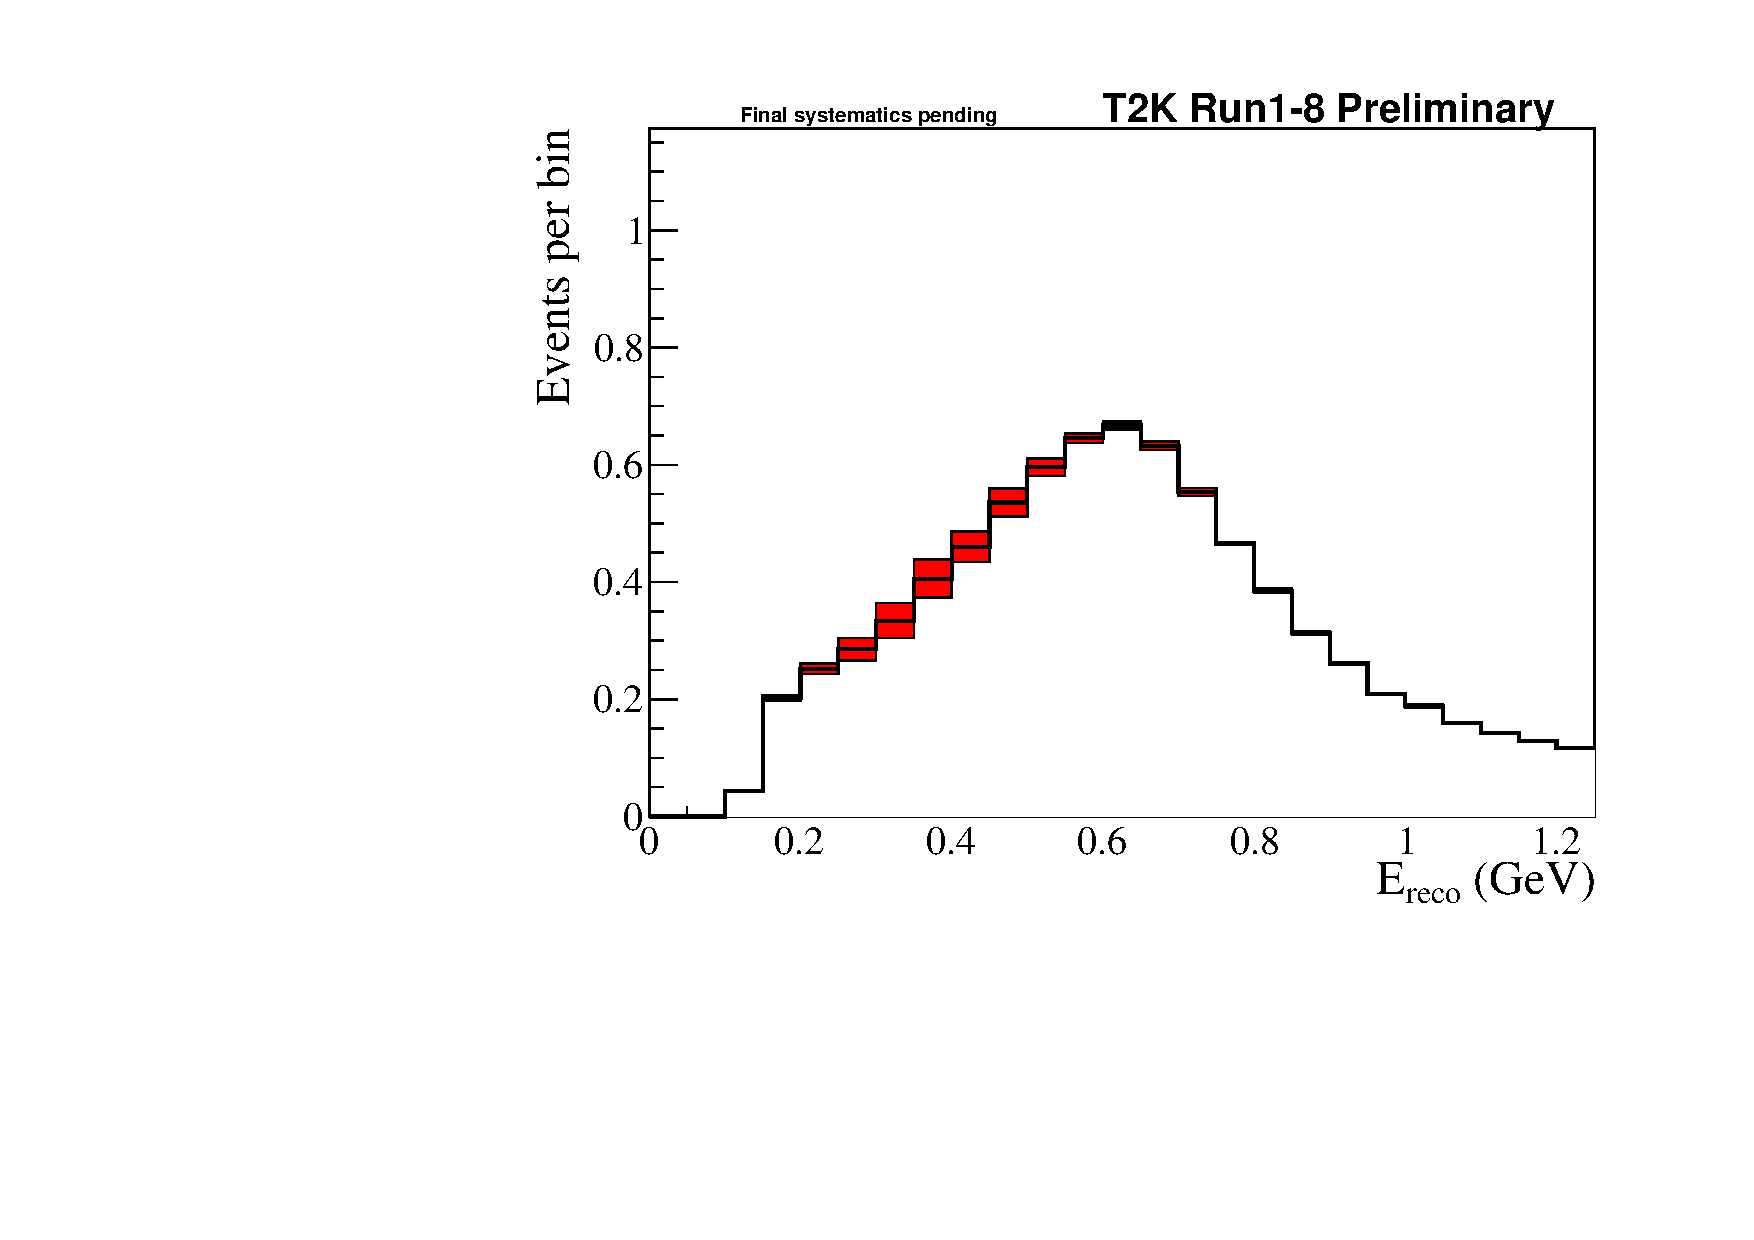
\includegraphics[width=0.9\textwidth]{systematics/envelopes/sk_errors/sk_error_table_RHC1Re_xsec_ncgamma_envelope}
		\caption{Electron-like antineutrino mode}
	\end{subfigure}
	\begin{subfigure}[b]{0.49\textwidth}
		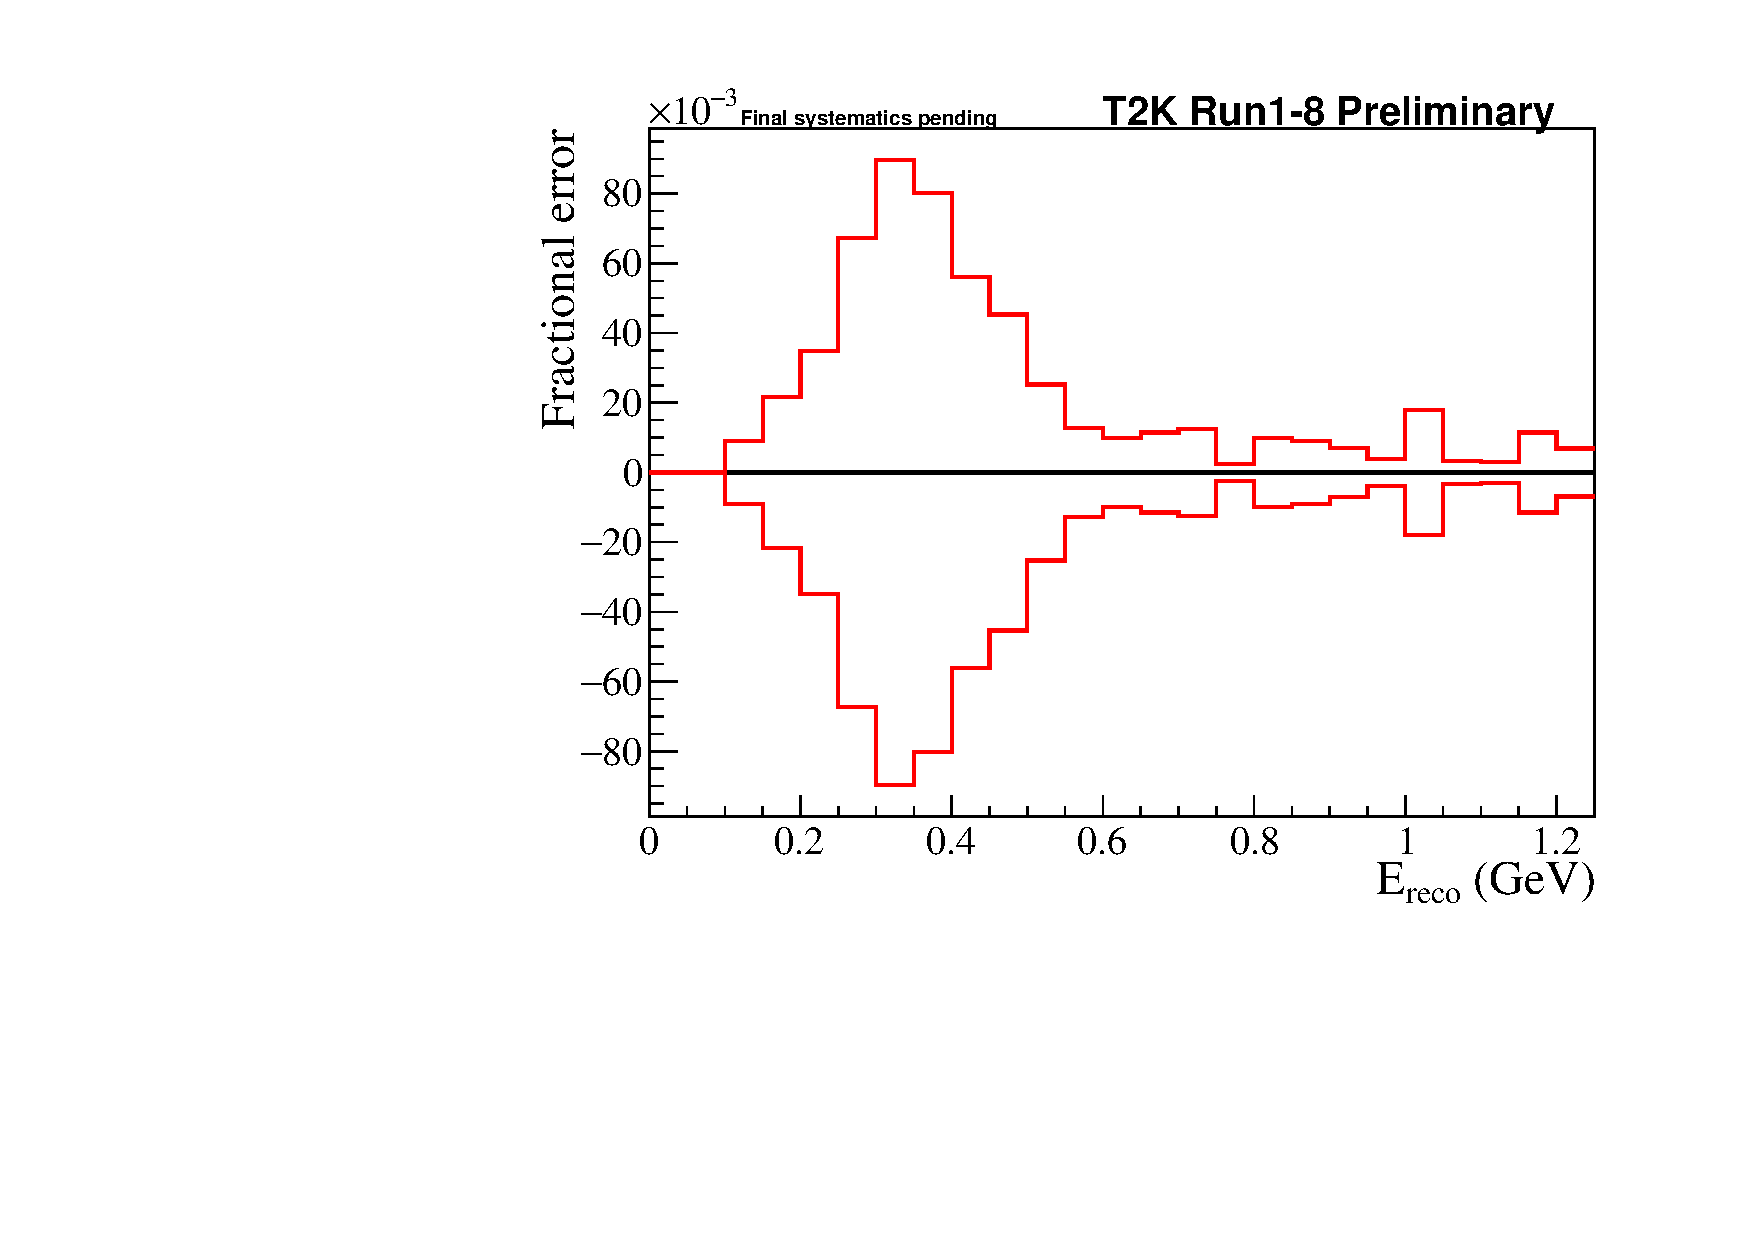
\includegraphics[width=0.9\textwidth]{systematics/envelopes/sk_errors/sk_error_table_RHC1Re_xsec_ncgamma_envelope_fractional}
		\caption{Electron-like antineutrino mode}
	\end{subfigure}
	\caption {
		Error envelopes (left) and fractional errors (right) for the reconstructed neutrino energy spectrum for the unconstrained NC$1\gamma$ systematic parameters. \num{1e4} toys are generated for the Asimov data set A with randomized systematic parameters with correlations taken into account.
	}
	\label{fig:sk_envelopes_xsec_ncgamma_b}
\end{figure*}
\clearpage
\begin{figure*}
	\center
	\begin{subfigure}[b]{0.49\textwidth}
		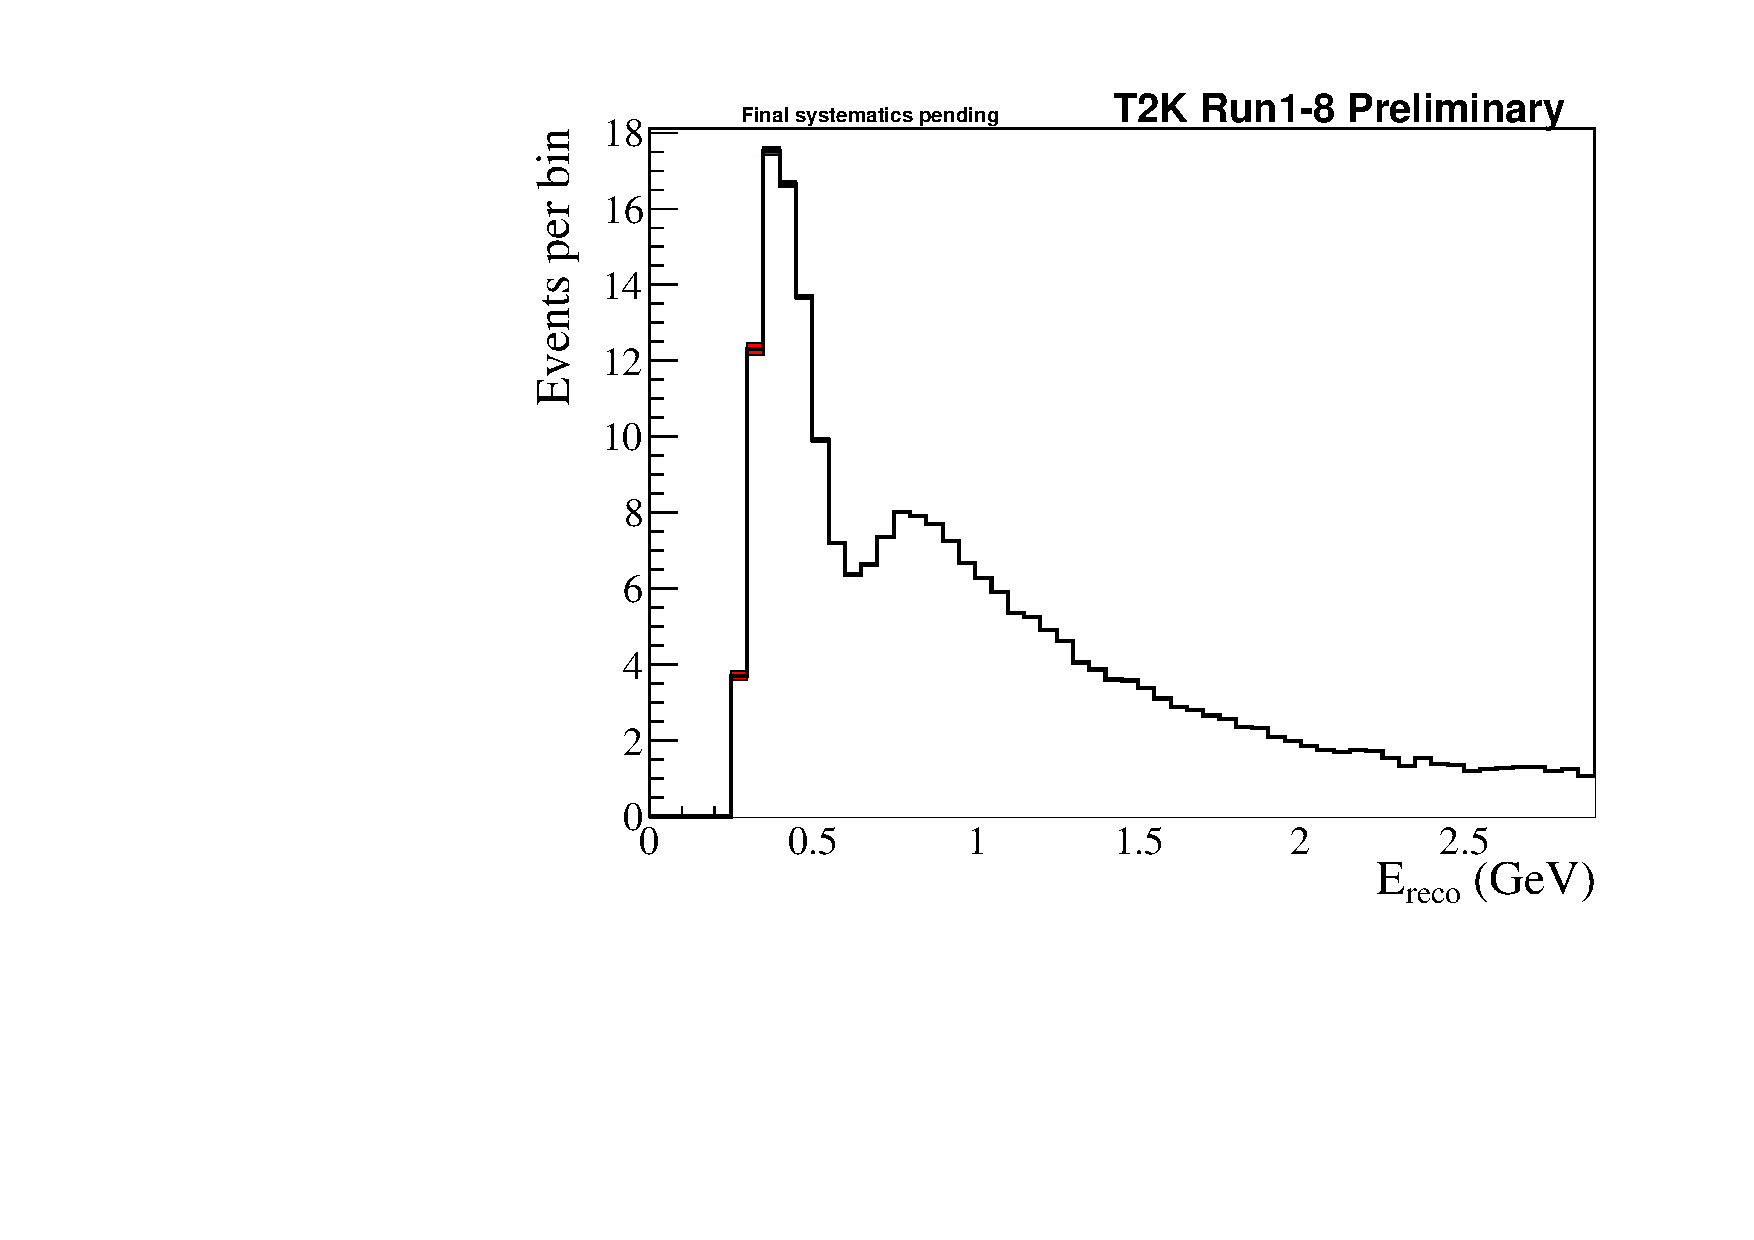
\includegraphics[width=0.9\textwidth]{systematics/envelopes/sk_errors/sk_error_table_1Rmu_xsec_ncoth_envelope}
		\caption{Muon-like, neutrino mode}
	\end{subfigure}
	\begin{subfigure}[b]{0.49\textwidth}
		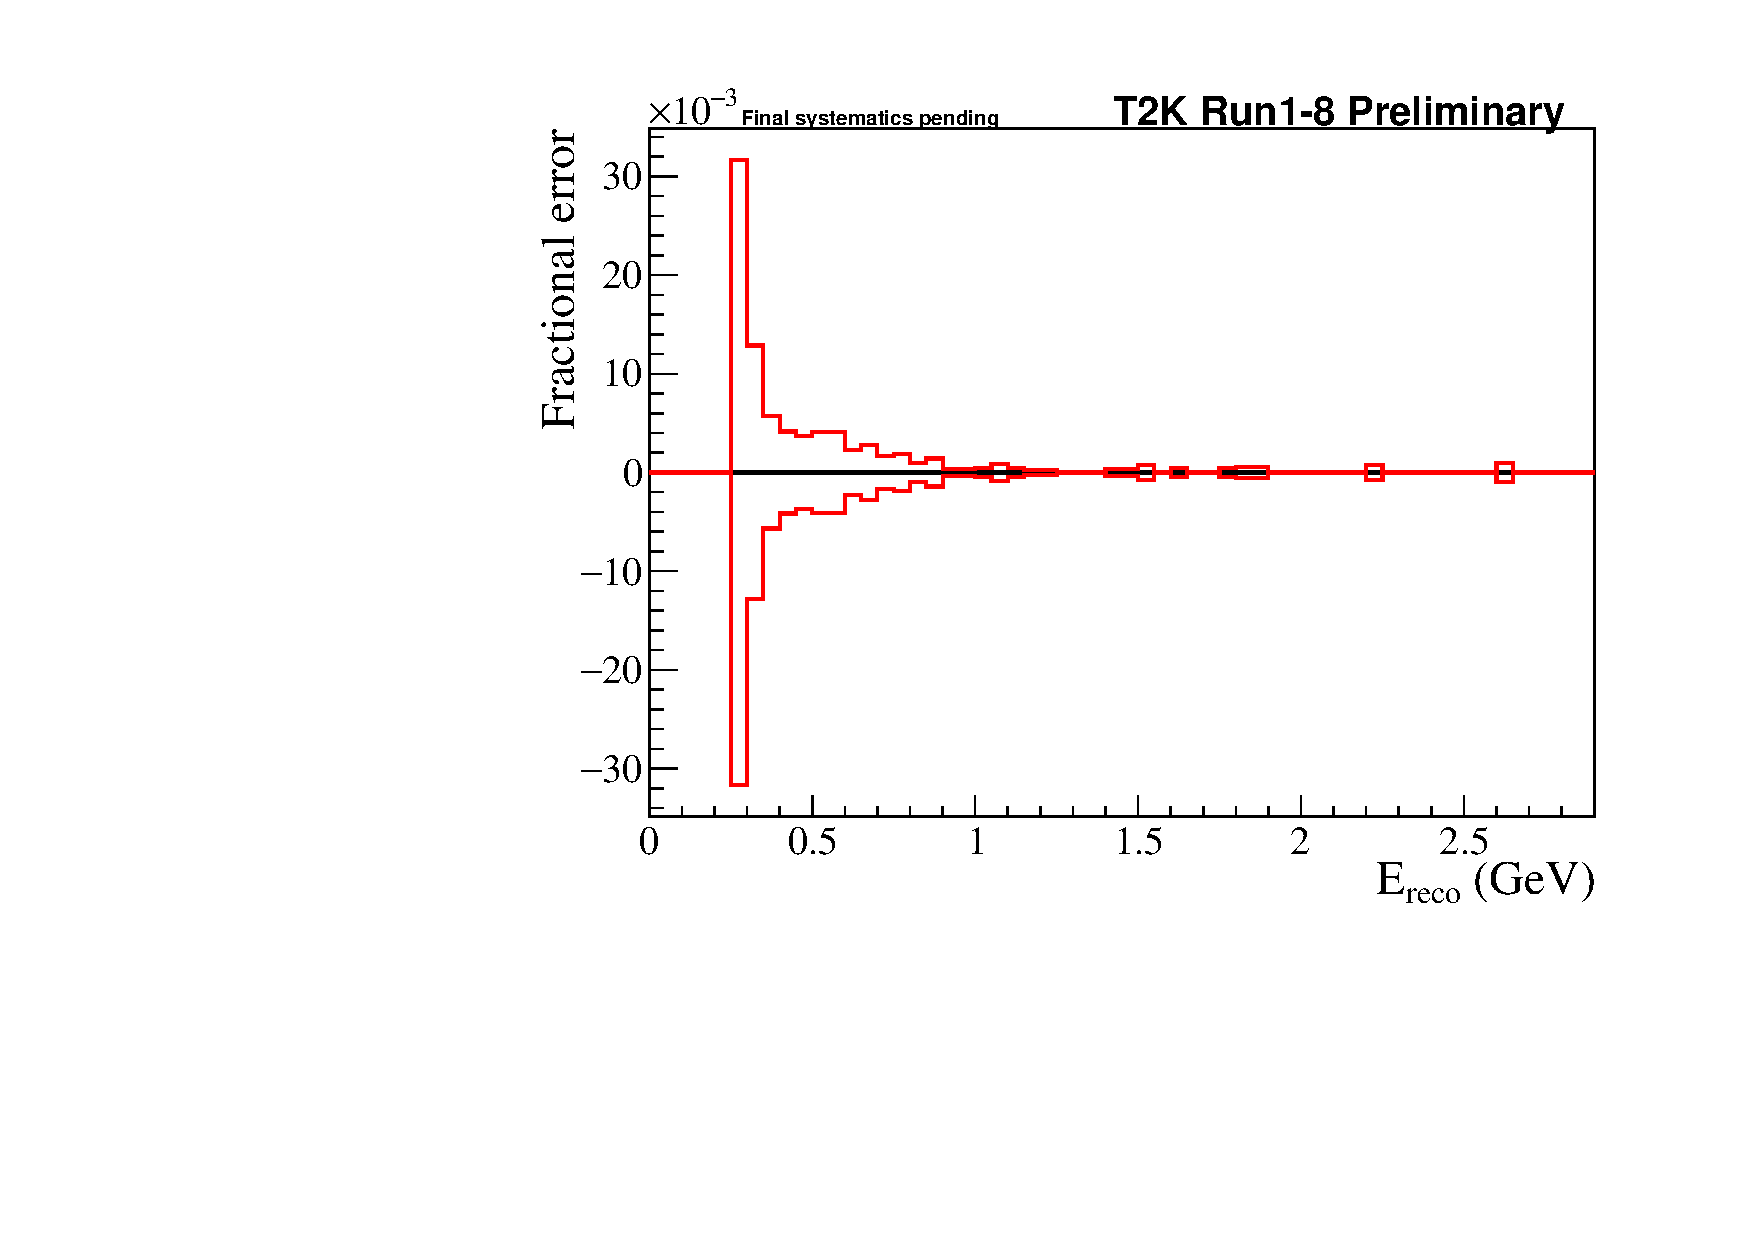
\includegraphics[width=0.9\textwidth]{systematics/envelopes/sk_errors/sk_error_table_1Rmu_xsec_ncoth_envelope_fractional}
		\caption{Muon-like, neutrino mode}
	\end{subfigure}
	\begin{subfigure}[b]{0.49\textwidth}
		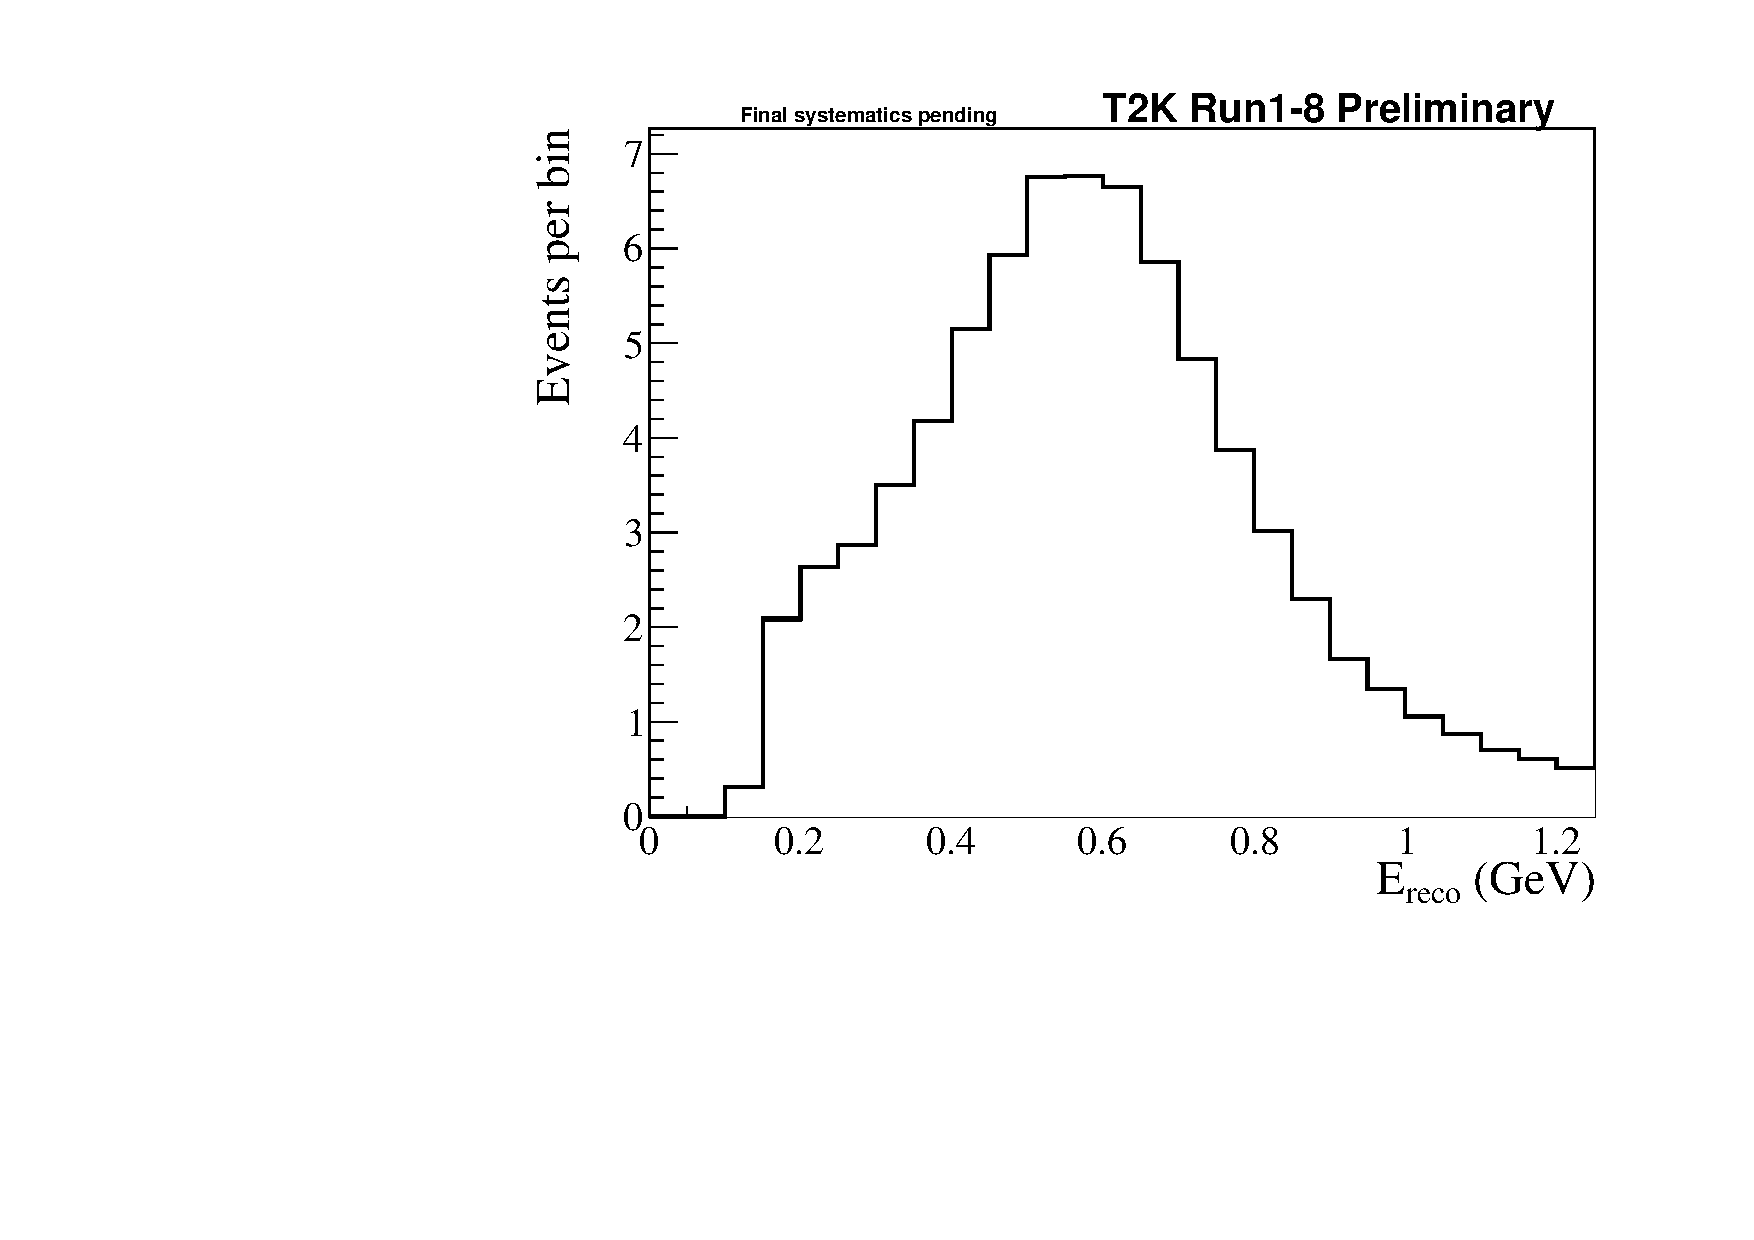
\includegraphics[width=0.9\textwidth]{systematics/envelopes/sk_errors/sk_error_table_1Re_xsec_ncoth_envelope}
		\caption{Electron-like, neutrino mode}
	\end{subfigure}
	\begin{subfigure}[b]{0.49\textwidth}
		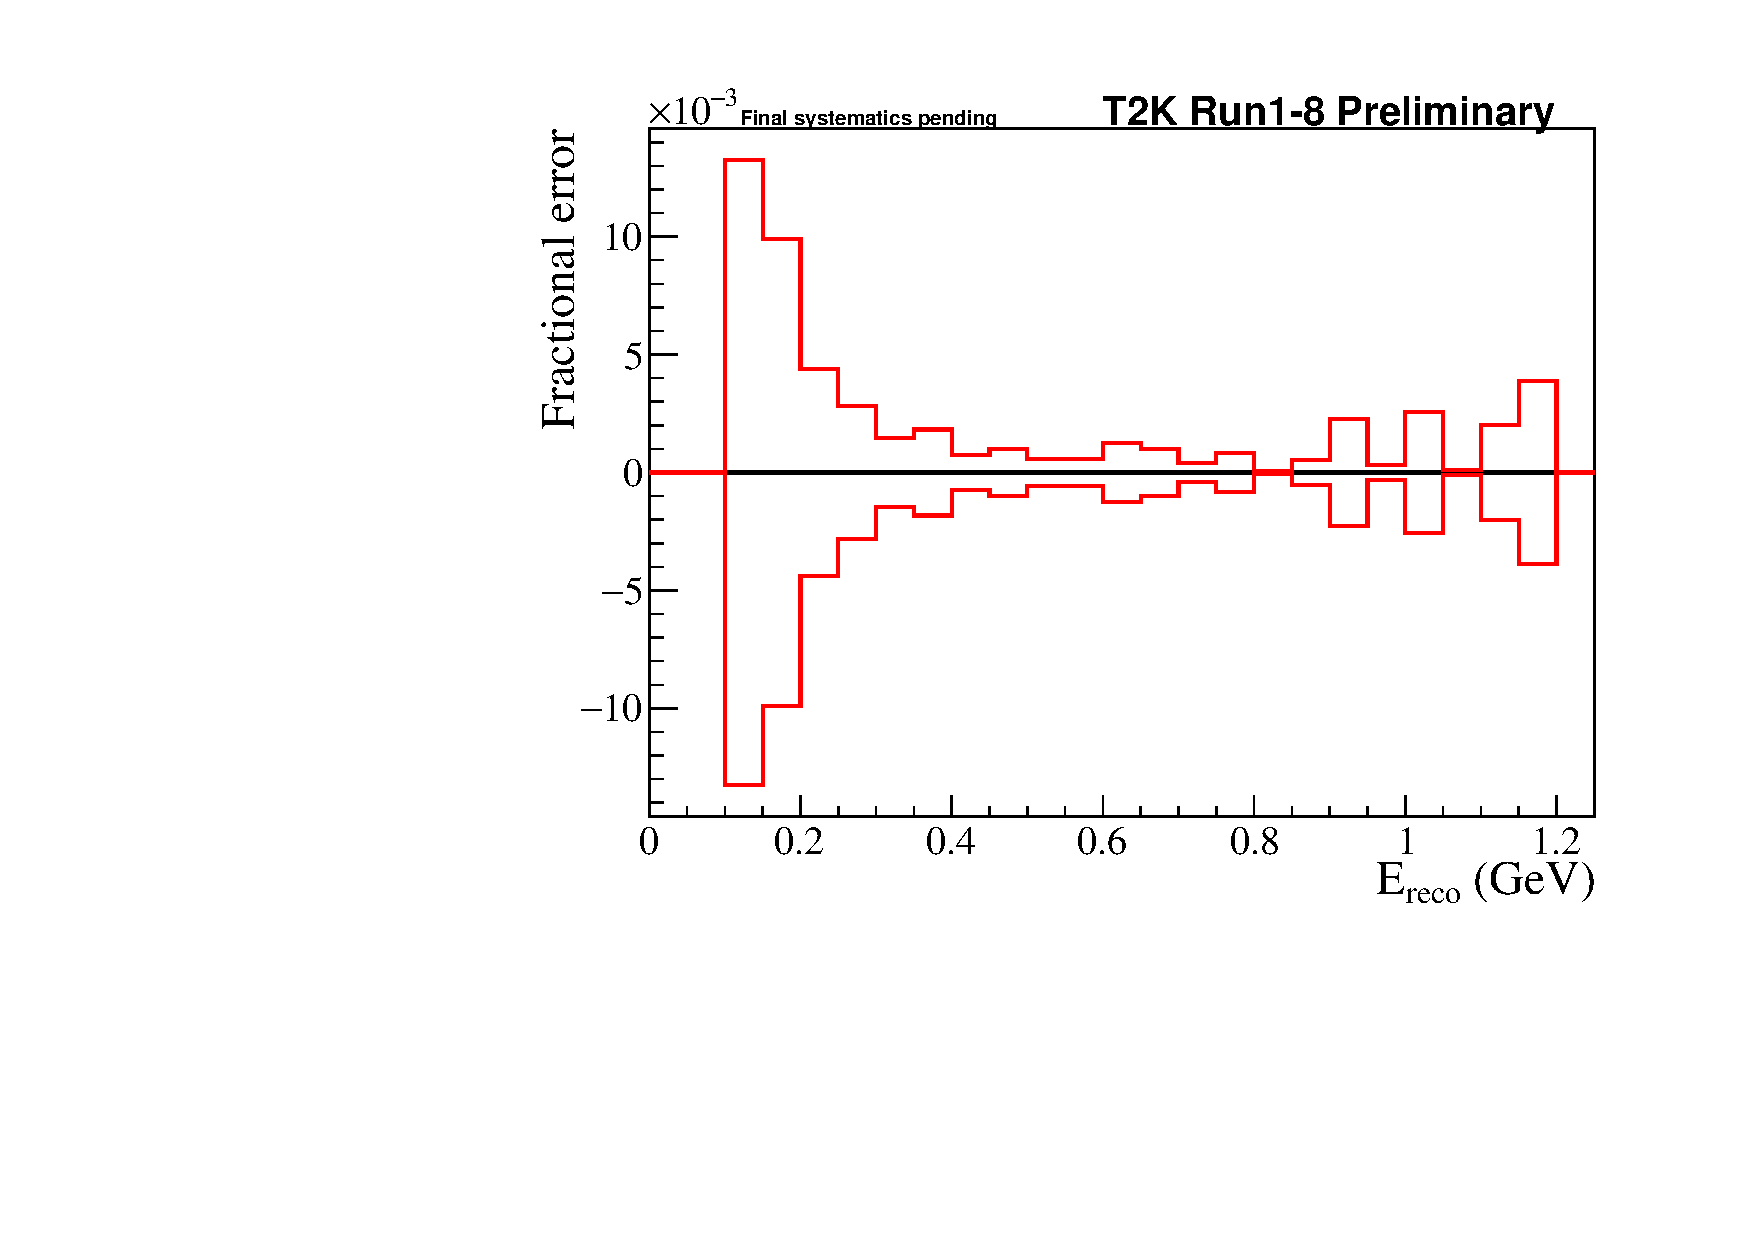
\includegraphics[width=0.9\textwidth]{systematics/envelopes/sk_errors/sk_error_table_1Re_xsec_ncoth_envelope_fractional}
		\caption{Electron-like, neutrino mode}
	\end{subfigure}
	\begin{subfigure}[b]{0.49\textwidth}
		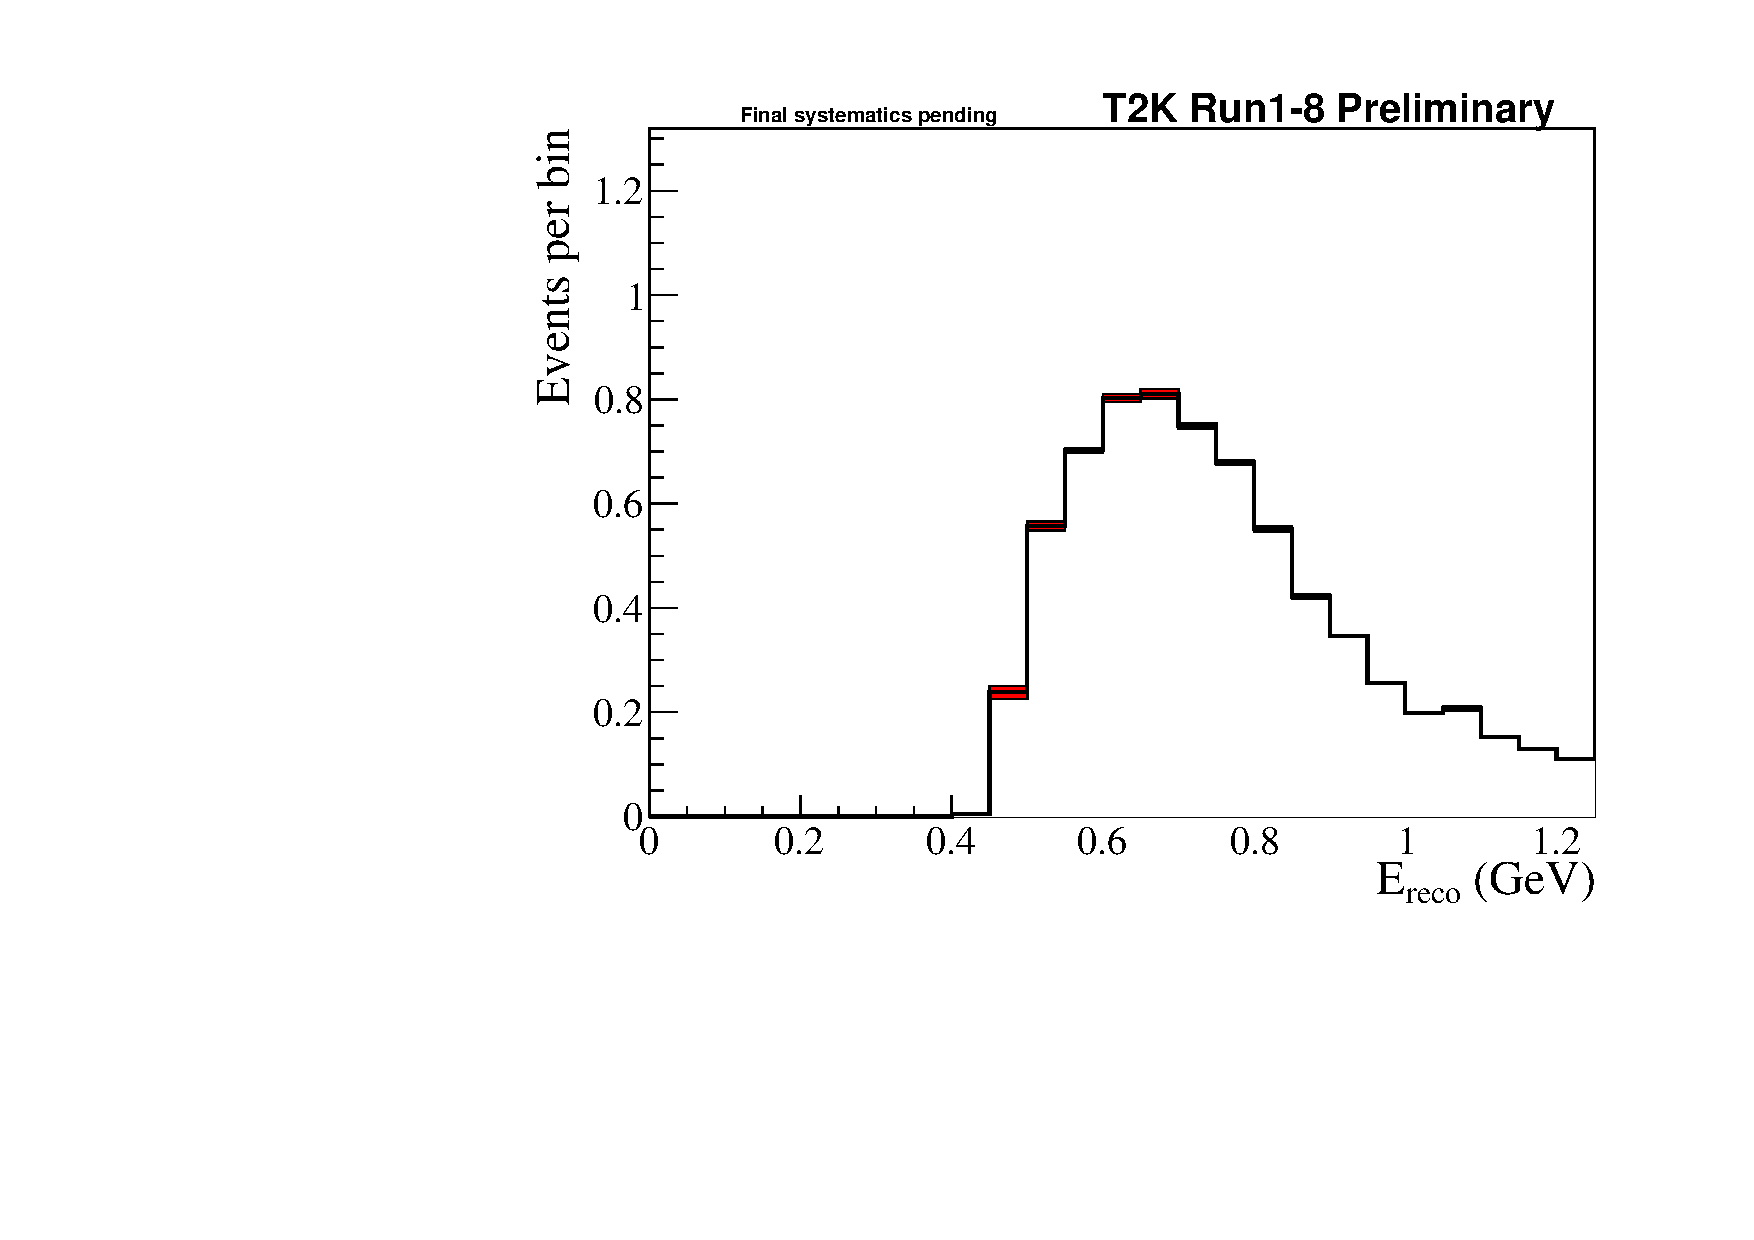
\includegraphics[width=0.9\textwidth]{systematics/envelopes/sk_errors/sk_error_table_MultiRe_xsec_ncoth_envelope}
		\caption{\nueCConepi-like, neutrino mode}
	\end{subfigure}
	\begin{subfigure}[b]{0.49\textwidth}
		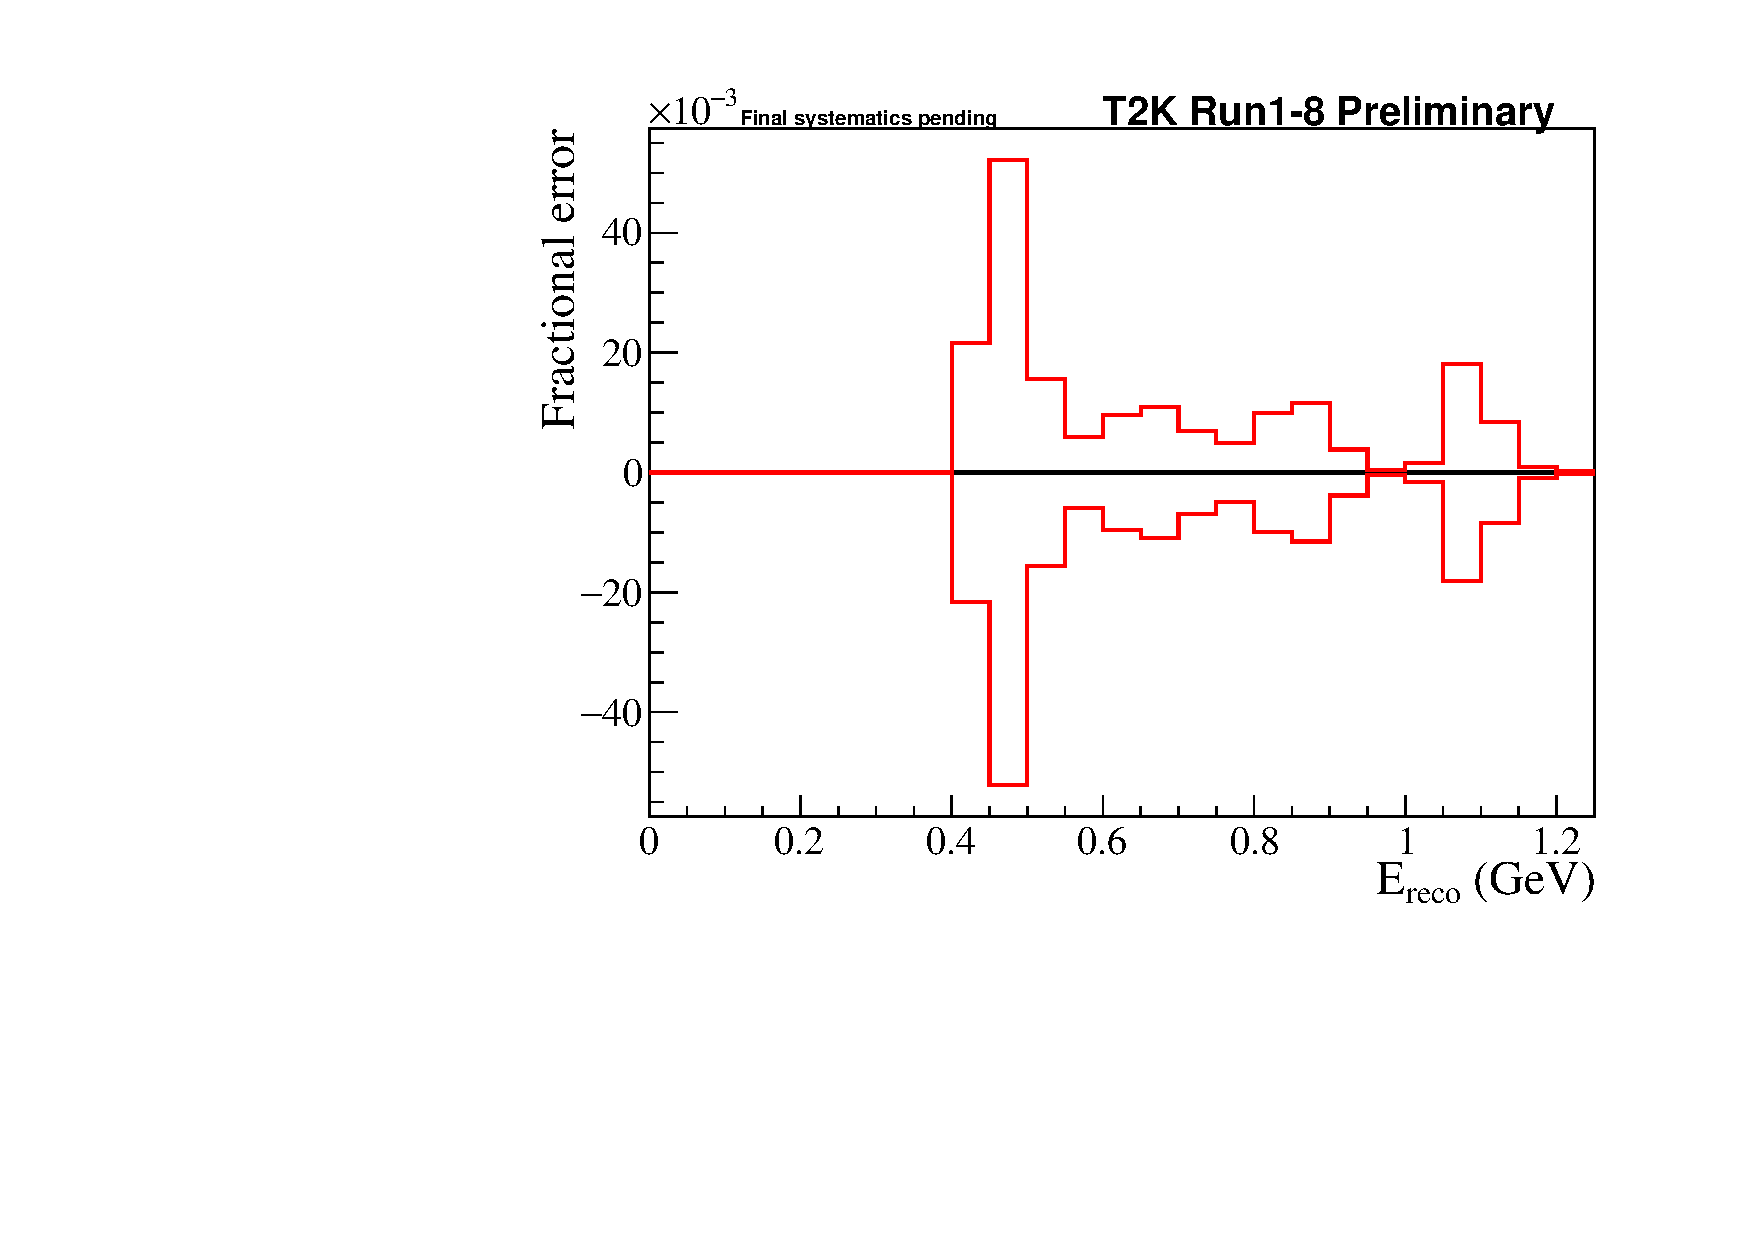
\includegraphics[width=0.9\textwidth]{systematics/envelopes/sk_errors/sk_error_table_MultiRe_xsec_ncoth_envelope_fractional}
		\caption{\nueCConepi-like, neutrino mode}
	\end{subfigure}
	\caption {
		Error envelopes (left) and fractional errors (right) for the reconstructed neutrino energy spectrum for the unconstrained NCother systematic parameters. \num{1e4} toys are generated for the Asimov data set A with randomized systematic parameters with correlations taken into account.
	}
	\label{fig:sk_envelopes_xsec_ncoth}
\end{figure*}
\clearpage

\begin{figure*}
	\center
	\begin{subfigure}[b]{0.49\textwidth}
		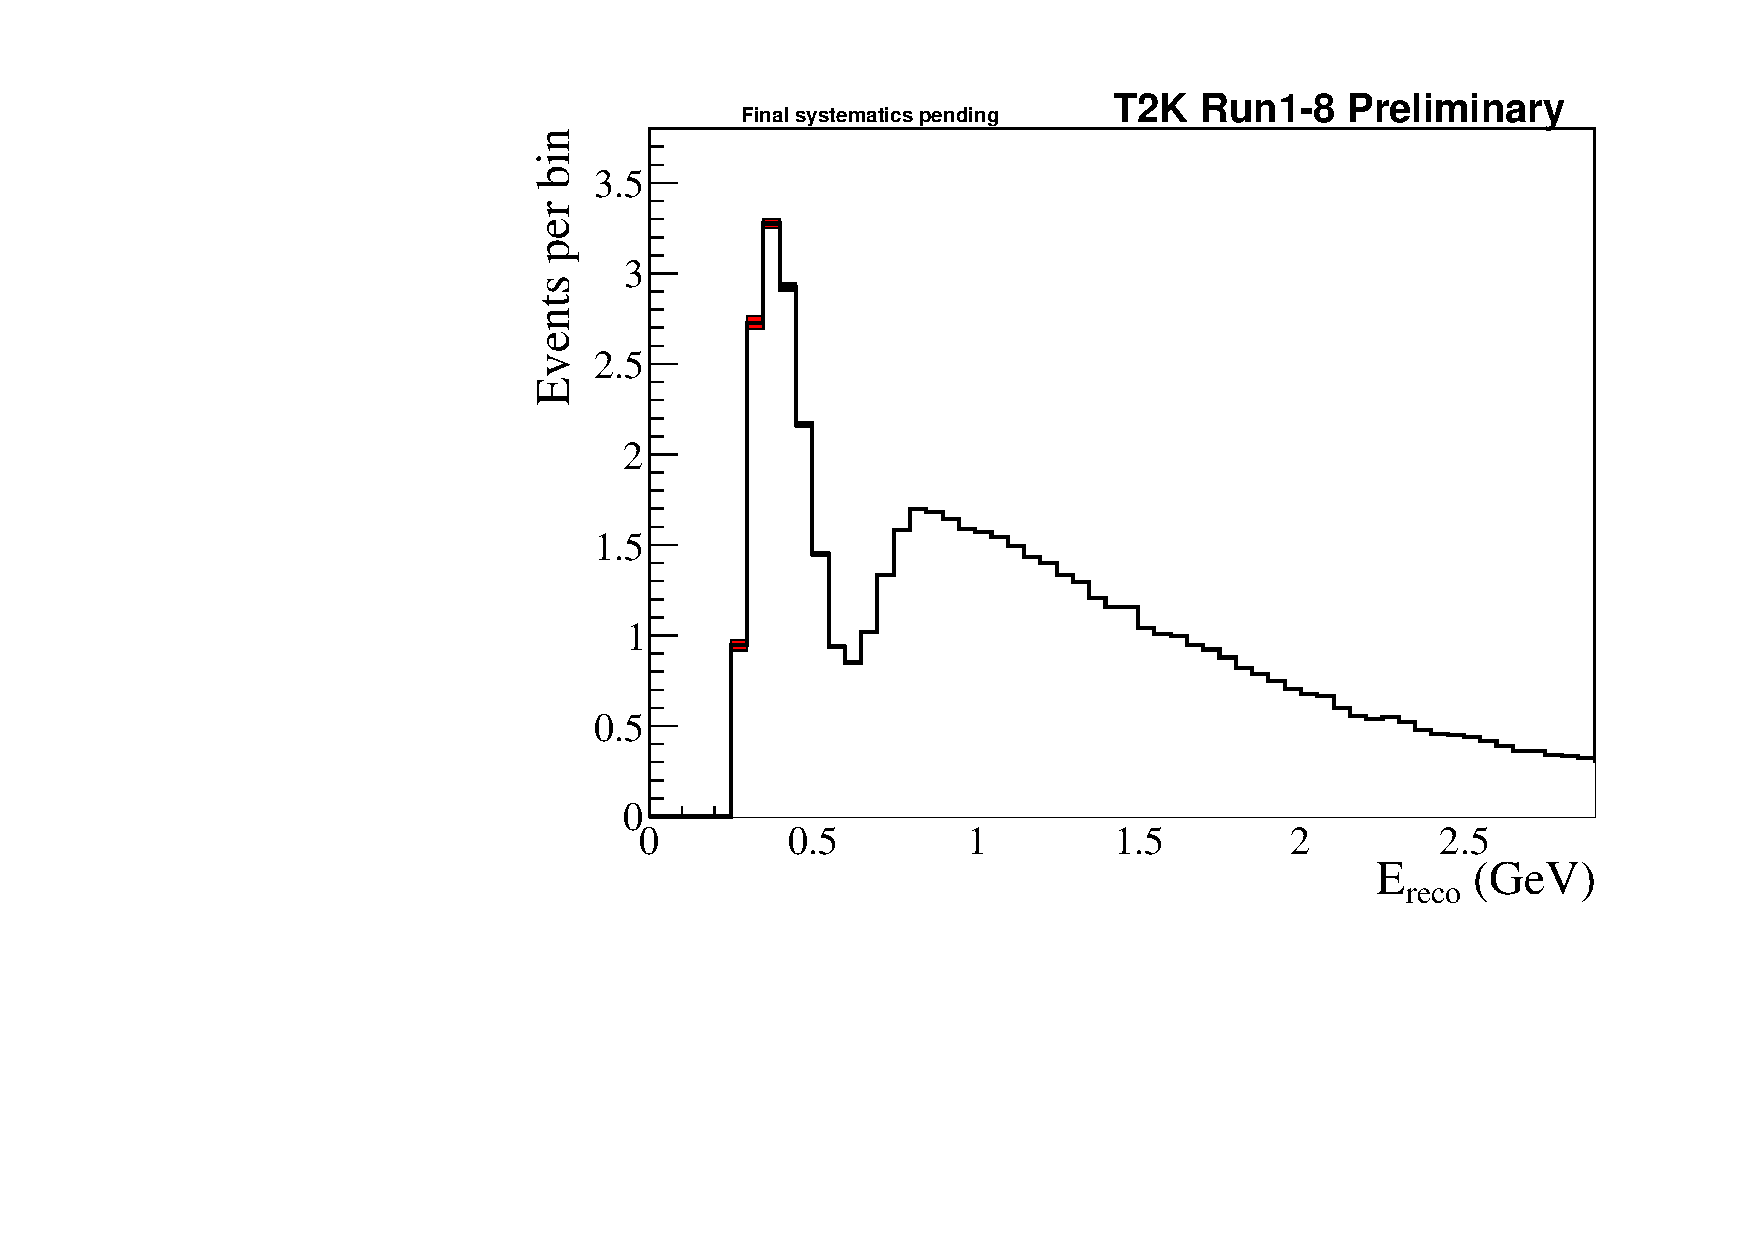
\includegraphics[width=0.9\textwidth]{systematics/envelopes/sk_errors/sk_error_table_RHC1Rmu_xsec_ncoth_envelope}
		\caption{Muon-like, antineutrino mode}
	\end{subfigure}
	\begin{subfigure}[b]{0.49\textwidth}
		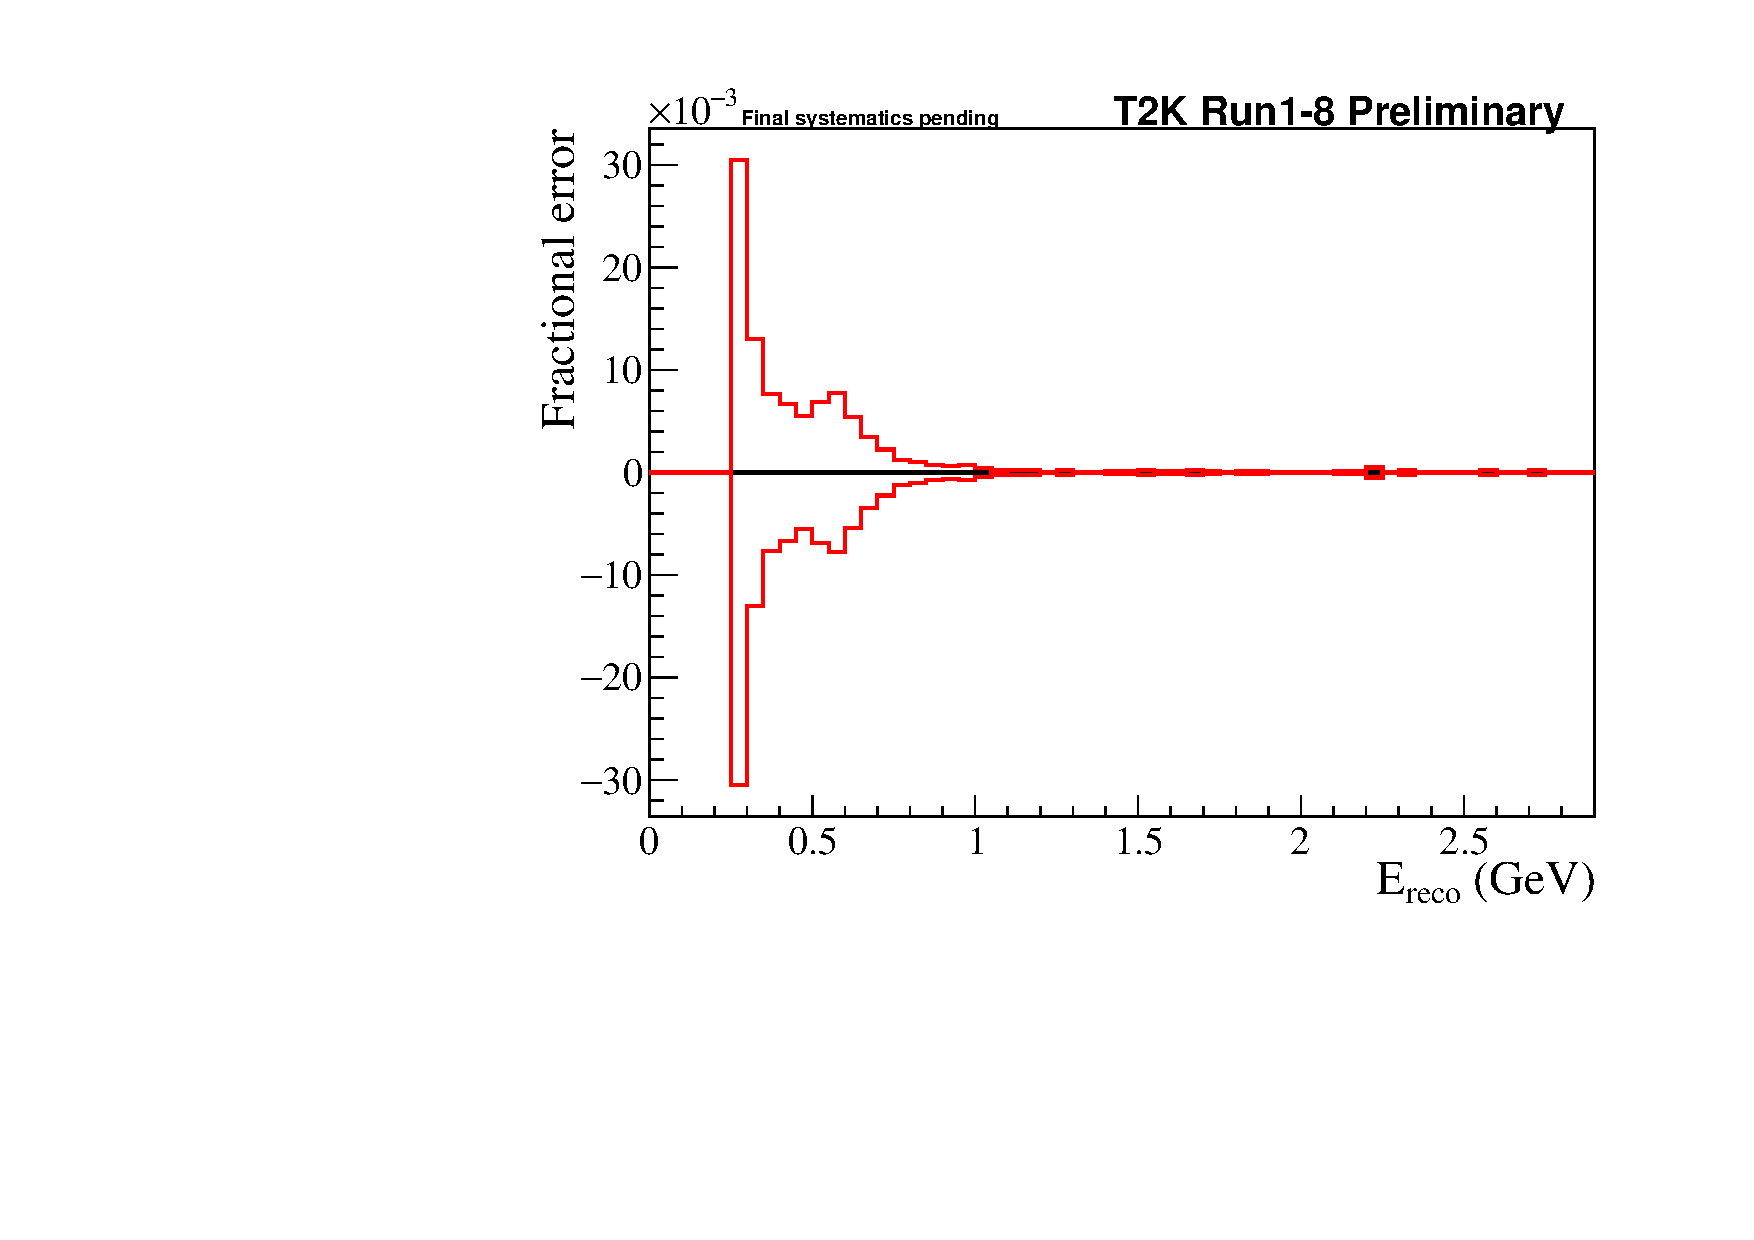
\includegraphics[width=0.9\textwidth]{systematics/envelopes/sk_errors/sk_error_table_RHC1Rmu_xsec_ncoth_envelope_fractional}
		\caption{Muon-like, antineutrino mode}
	\end{subfigure}
	\begin{subfigure}[b]{0.49\textwidth}
		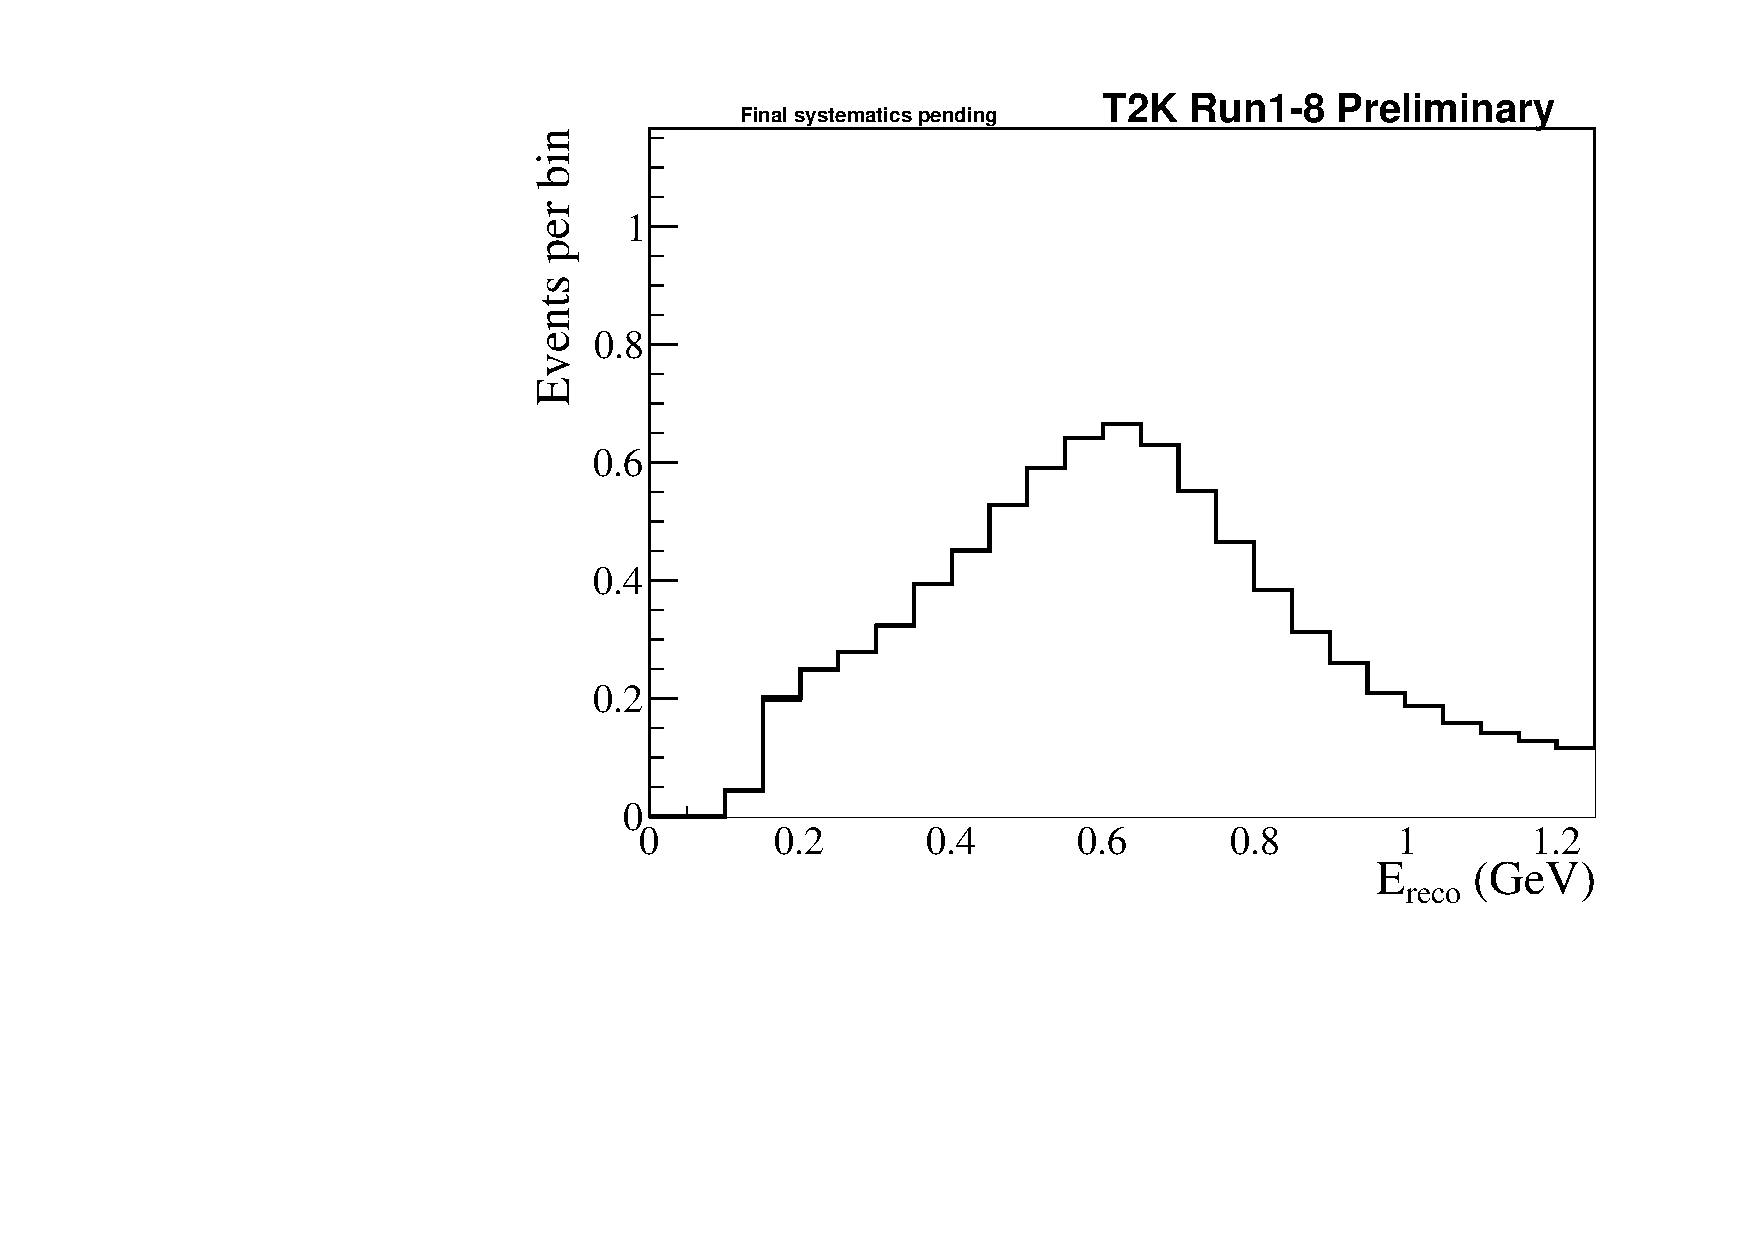
\includegraphics[width=0.9\textwidth]{systematics/envelopes/sk_errors/sk_error_table_RHC1Re_xsec_ncoth_envelope}
		\caption{Electron-like antineutrino mode}
	\end{subfigure}
	\begin{subfigure}[b]{0.49\textwidth}
		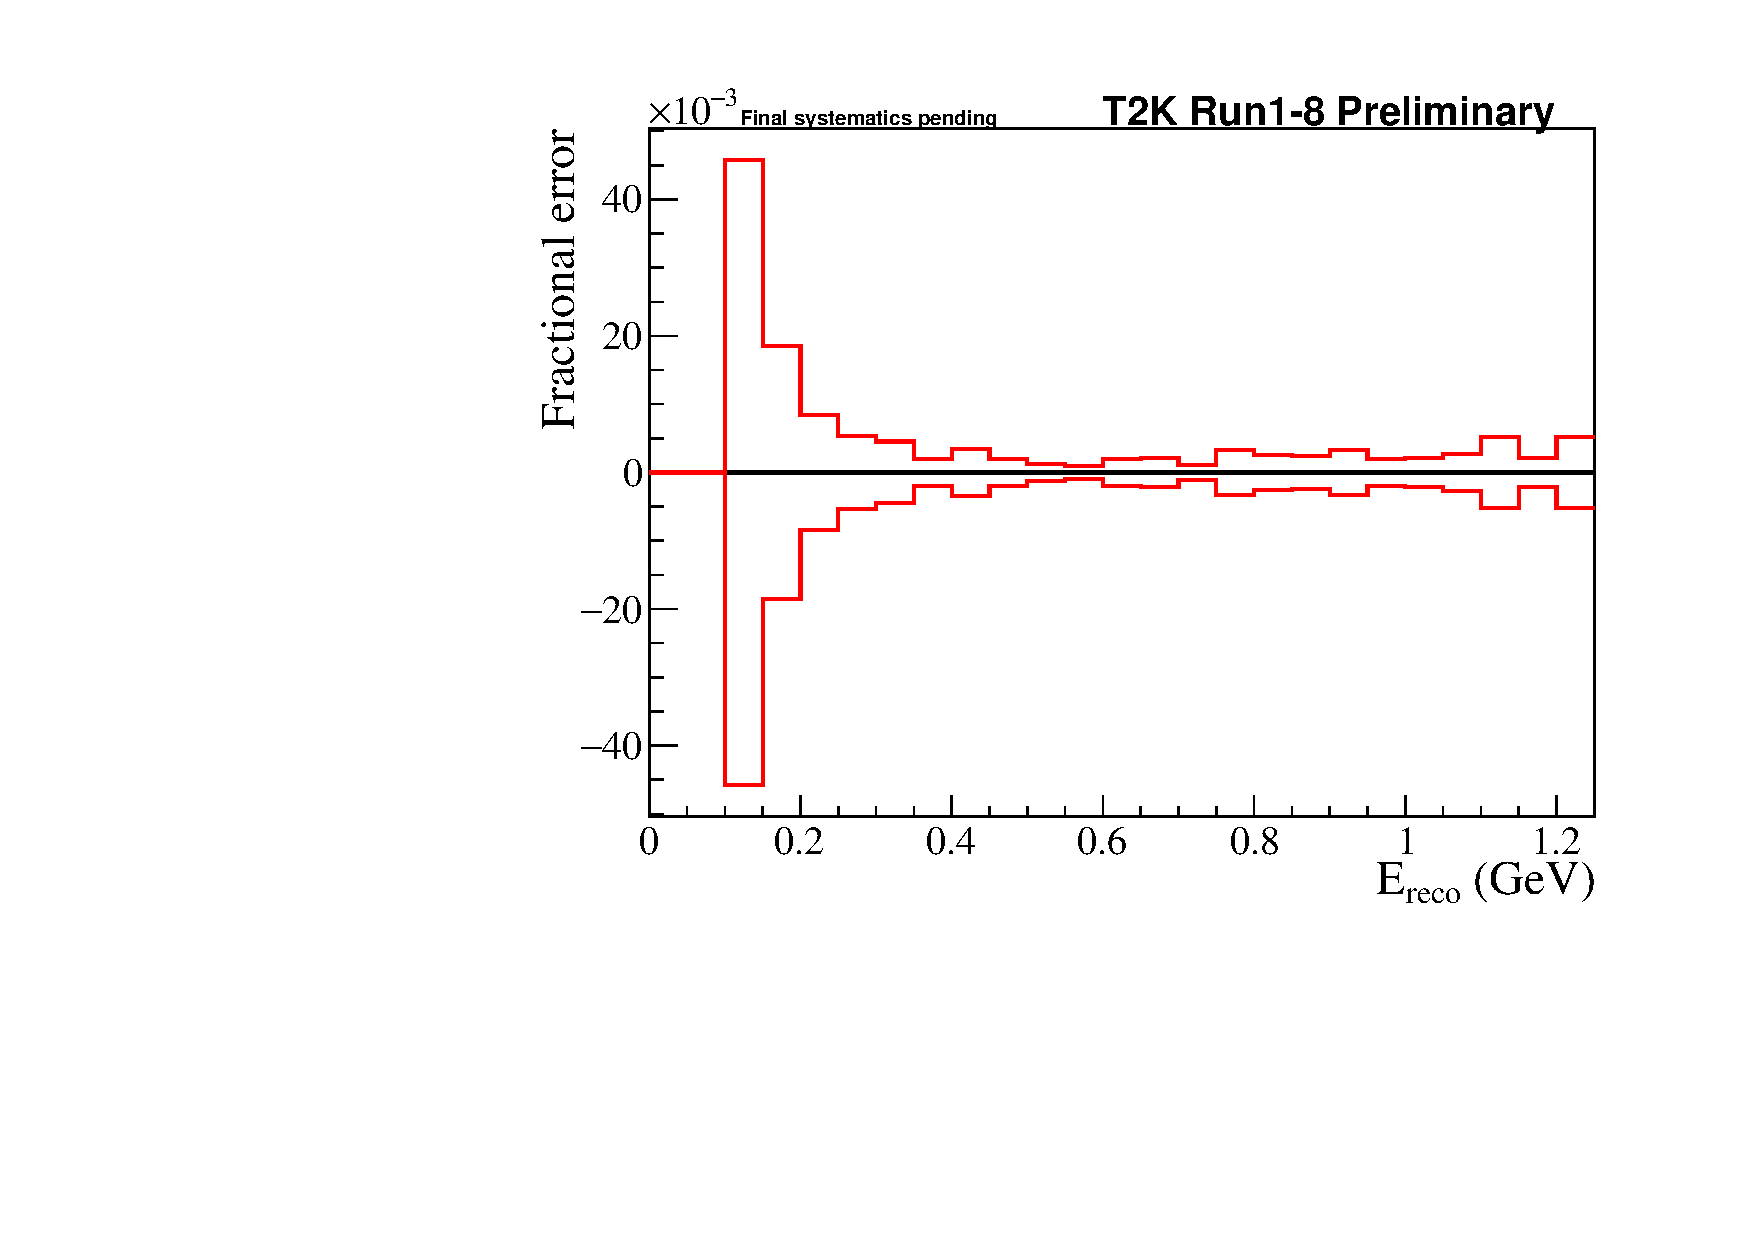
\includegraphics[width=0.9\textwidth]{systematics/envelopes/sk_errors/sk_error_table_RHC1Re_xsec_ncoth_envelope_fractional}
		\caption{Electron-like antineutrino mode}
	\end{subfigure}
	\caption {
		Error envelopes (left) and fractional errors (right) for the reconstructed neutrino energy spectrum for the unconstrained NCother systematic parameters. \num{1e4} toys are generated for the Asimov data set A with randomized systematic parameters with correlations taken into account.
	}
	\label{fig:sk_envelopes_xsec_ncoth_b}
\end{figure*}
\clearpage

\clearpage


%..................

%%% Local Variables:
%%% mode: latex
%%% TeX-master: "../TN327"
%%% End:

\clearpage

\section {Sensitivity studies}
\label{sec:sensitivity}
To determine the sensitivity of the analysis a number of fits were performed using Asimov data set A, the contours for which indicate the ability of the analysis to measure the oscillation parameters in the absence of statistical fluctuations and under the assumption that their true values correspond to the Asimov A values. Fits of single parameters are performed for each of \ssqthonethree, \deltacp, \ssqthtwothree and \dmsqtwothree, with two-dimensional fits being performed for \appearance and \disappearance. Fits are performed for each of normal and inverted hierarchy, and also with and without the reactor constraint on \ssqthonethree.

\subsection {Asimov data sets}
\label{sec:sensitivity:asimov_data_sets}
The definitions of the Asimov data sets given in \cref{sec:asimov_definition} are repeated here for reference.
\begin{table}[H]
\centering
\begin{tabular}{| c | c | c |}
\hline
Parameter(s) &	Asimov A & Asimov B	\\
\hline
$\sin^{2}\theta_{23}$	&	0.528	&  0.450	\\%0.624	\\
$\sin^{2} \theta_{13}$ reactors	&	0.0219	&	0.0219	\\
$\sin^{2} \theta_{12}$	&	0.304	&	0.304	\\
$|\Delta m^{2}_{32}|$ (NH) / $|\Delta m^{2}_{31}|$ (IH)	&	$2.509 \times 10^{-3}~\mbox{eV}^2/\mbox{c}^4$	&	$2.509 \times 10^{-3}~\mbox{eV}^2/\mbox{c}^4$	\\
$\Delta m^{2}_{21}$	&	$7.53 \times 10^{-5}~\mbox{eV}^2/\mbox{c}^4$	&	$7.53 \times 10^{-5}~\mbox{eV}^2/\mbox{c}^4$	\\
$\delta_{CP}$	&	-1.601	&	0	\\
Mass Hierarchy	&	Normal	&	Normal	\\  
\hline
\end{tabular}
\caption{
Values of oscillation parameters used to compute the event rates, systematic effects and sensitivity studies. Each set of oscillation parameters correspond to a different Asimov data set, which is the MC expected distribution in a certain oscillation hypothesis.
In the Asimov data set A the nominal values of $\sin^2 2 \theta_{13}$, $\sin^2 2 \theta_{12}$ and $\Delta m^2_{21}$  are from \cite{pdg_2014}, while all the other oscillation parameter values corresponds to the most probable values obtained by the Bayesian analysis on the T2K run 1-4 neutrino mode data \cite{T2KLongPaper}. The mass hierarchy is not marginalised but fixed to either NH or IH.
}
\label{tab:asimov_definition2}
\end{table}
\clearpage
\subsection{Results for Asimov sets A and B}
\label{sec:sensitivity:asimov_results}

\subsubsection{Results for \appearance}
In \cref{fig:ssqth13_vs_dcp_sensitivity} the sensitivity to \appearance with reactor constraint and T2K only is shown for the Asimov data sets A and B. Note that in the Asimov B case it can be seen that the best-fit point is shifted away from the true \deltacp value of zero towards $-\pi$. In addition to best-fit points being moved from the true value due to marginalisation of oscillation and systematic parameters there are additional contributing effects. There is a lack of sensitivity to distinguish $\delta_{CP} = 0$ and $\delta_{CP} = \pi$ due to the spectra for $\delta_{CP} = 0$ in inverted hierarchy being similar to the spectra for $\delta_{CP} = \pi$ in normal hierarchy and vice versa (see \cref{fig:asimovb_spectra_degeneracy} in \cref{app:asimovb_sensitivity}), leading to similar $\Delta\chi^2$ values for the two points. This can be seen in \cref{fig:dcp_sensitivity}(c) and \cref{fig:dcp_sensitivity}(d), with the difference in $\Delta\chi^2_{true}$ and $\Delta\chi^2_{best-fit}$ being only $\sim 0.2$. Furthermore, degeneracy between \deltacp and mass hierarchy can cause $\delta_{CP} = 0$ to behave more like $\delta_{CP} = \pi/2$ in inverted hierarchy, and more like $\delta_{CP} = -\pi/2$ in normal hierarchy, shifting the best-fit for inverted hierarchy away from zero to a value between $-\pi$ and $-\pi/2$.

\begin{figure*}[htb]
	\center
	\begin{subfigure}[b]{0.49\textwidth}
		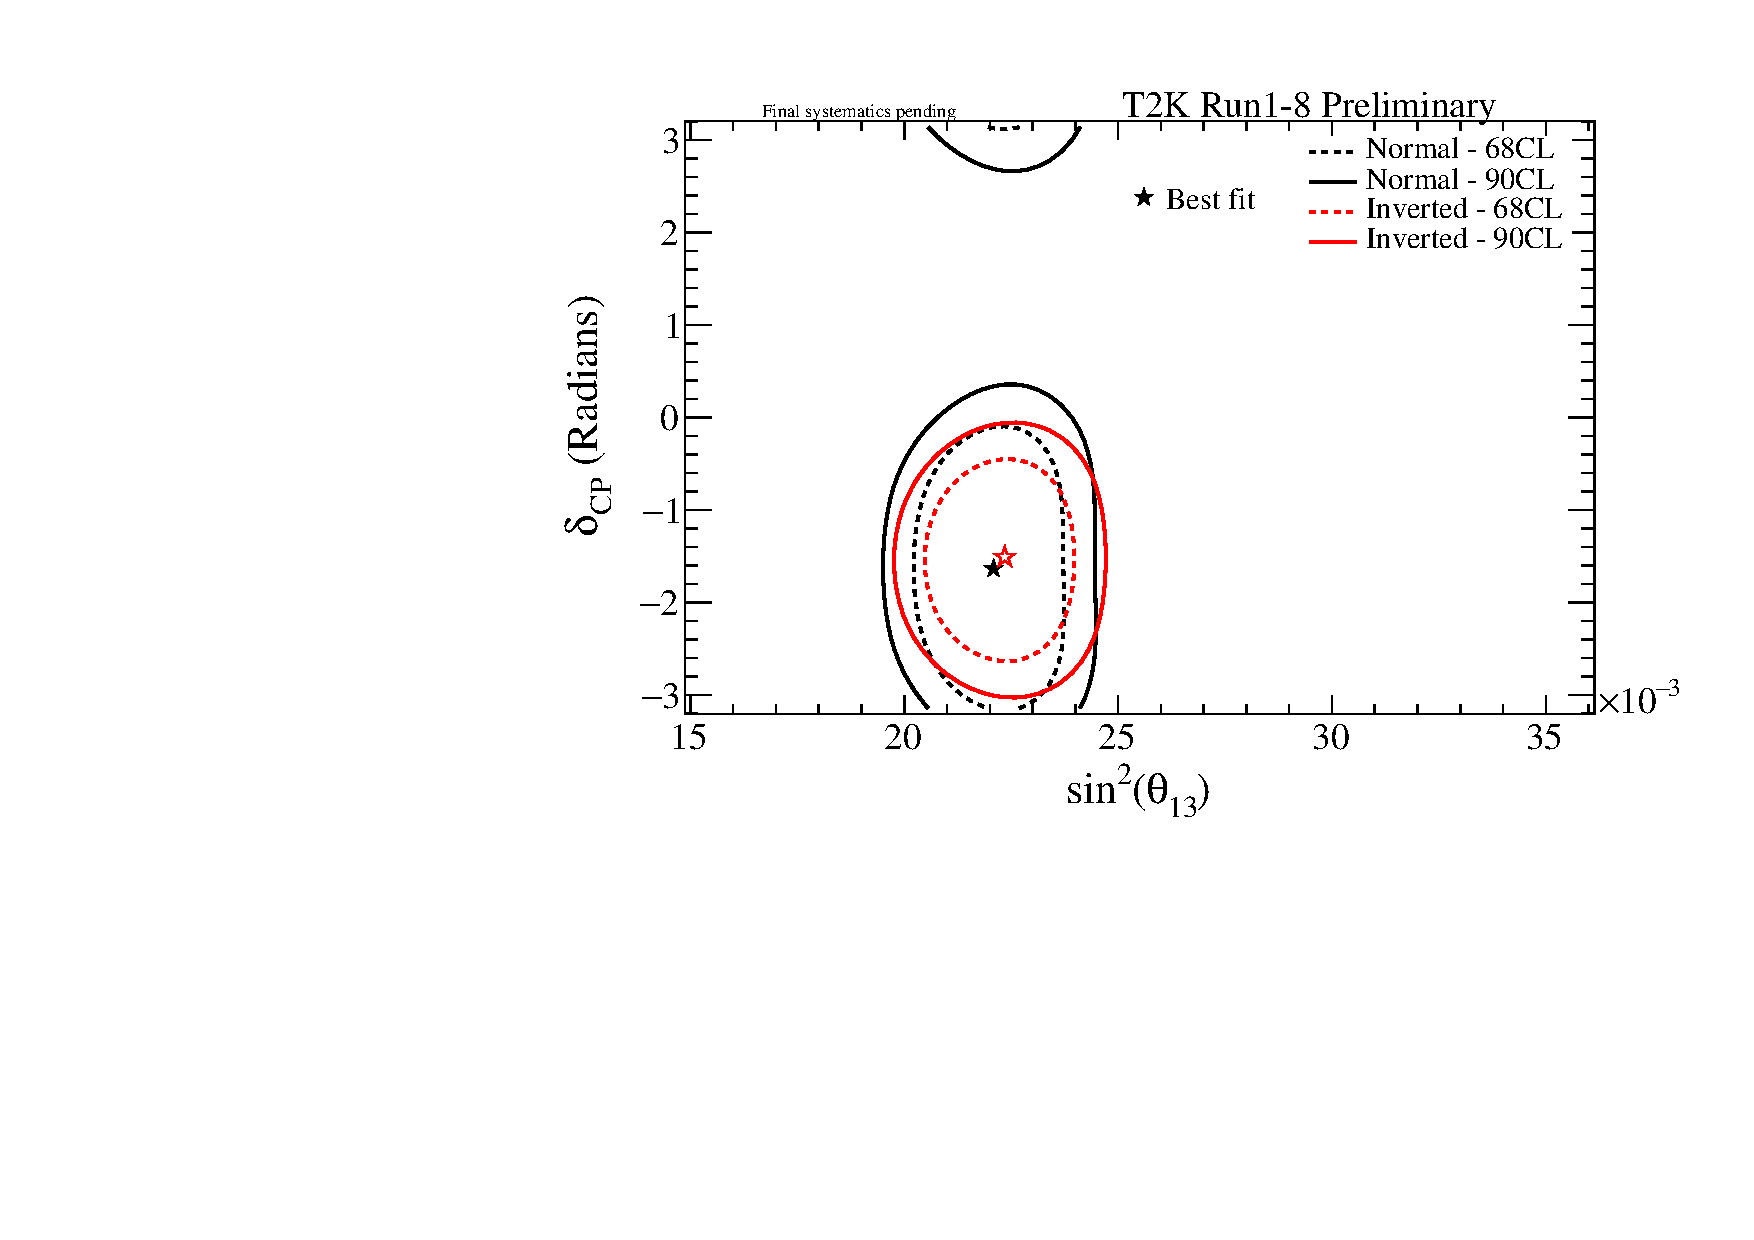
\includegraphics[width=0.9\textwidth]{sensitivity/reactor/mixing13_deltacp_AsimovA_reactor_global}
		\caption{Asimov A \appearance with reactor constraint}
	\end{subfigure}
	\begin{subfigure}[b]{0.49\textwidth}
		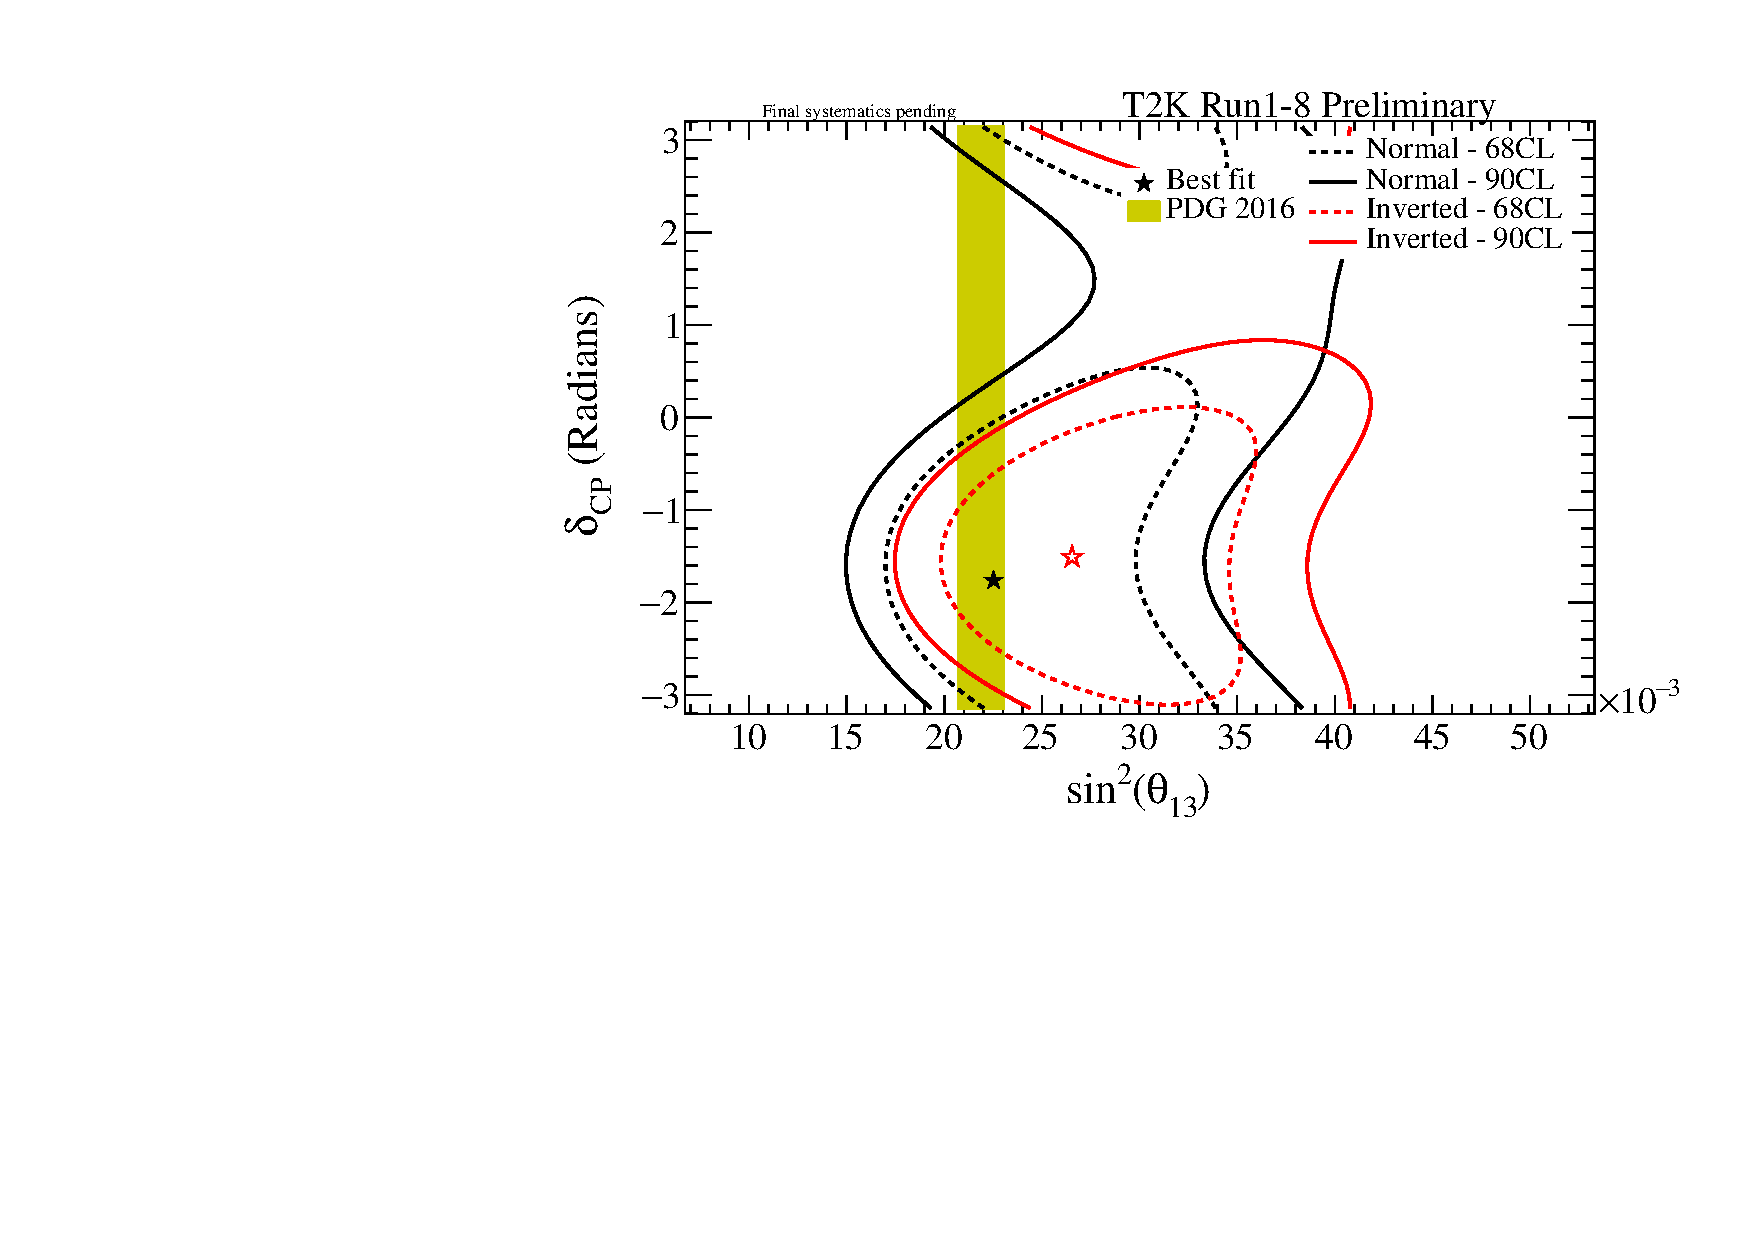
\includegraphics[width=0.9\textwidth]{sensitivity/t2k/mixing13_deltacp_AsimovA_t2k_global}
		\caption{Asimov A \appearance T2K only}
	\end{subfigure}
	\begin{subfigure}[b]{0.49\textwidth}
		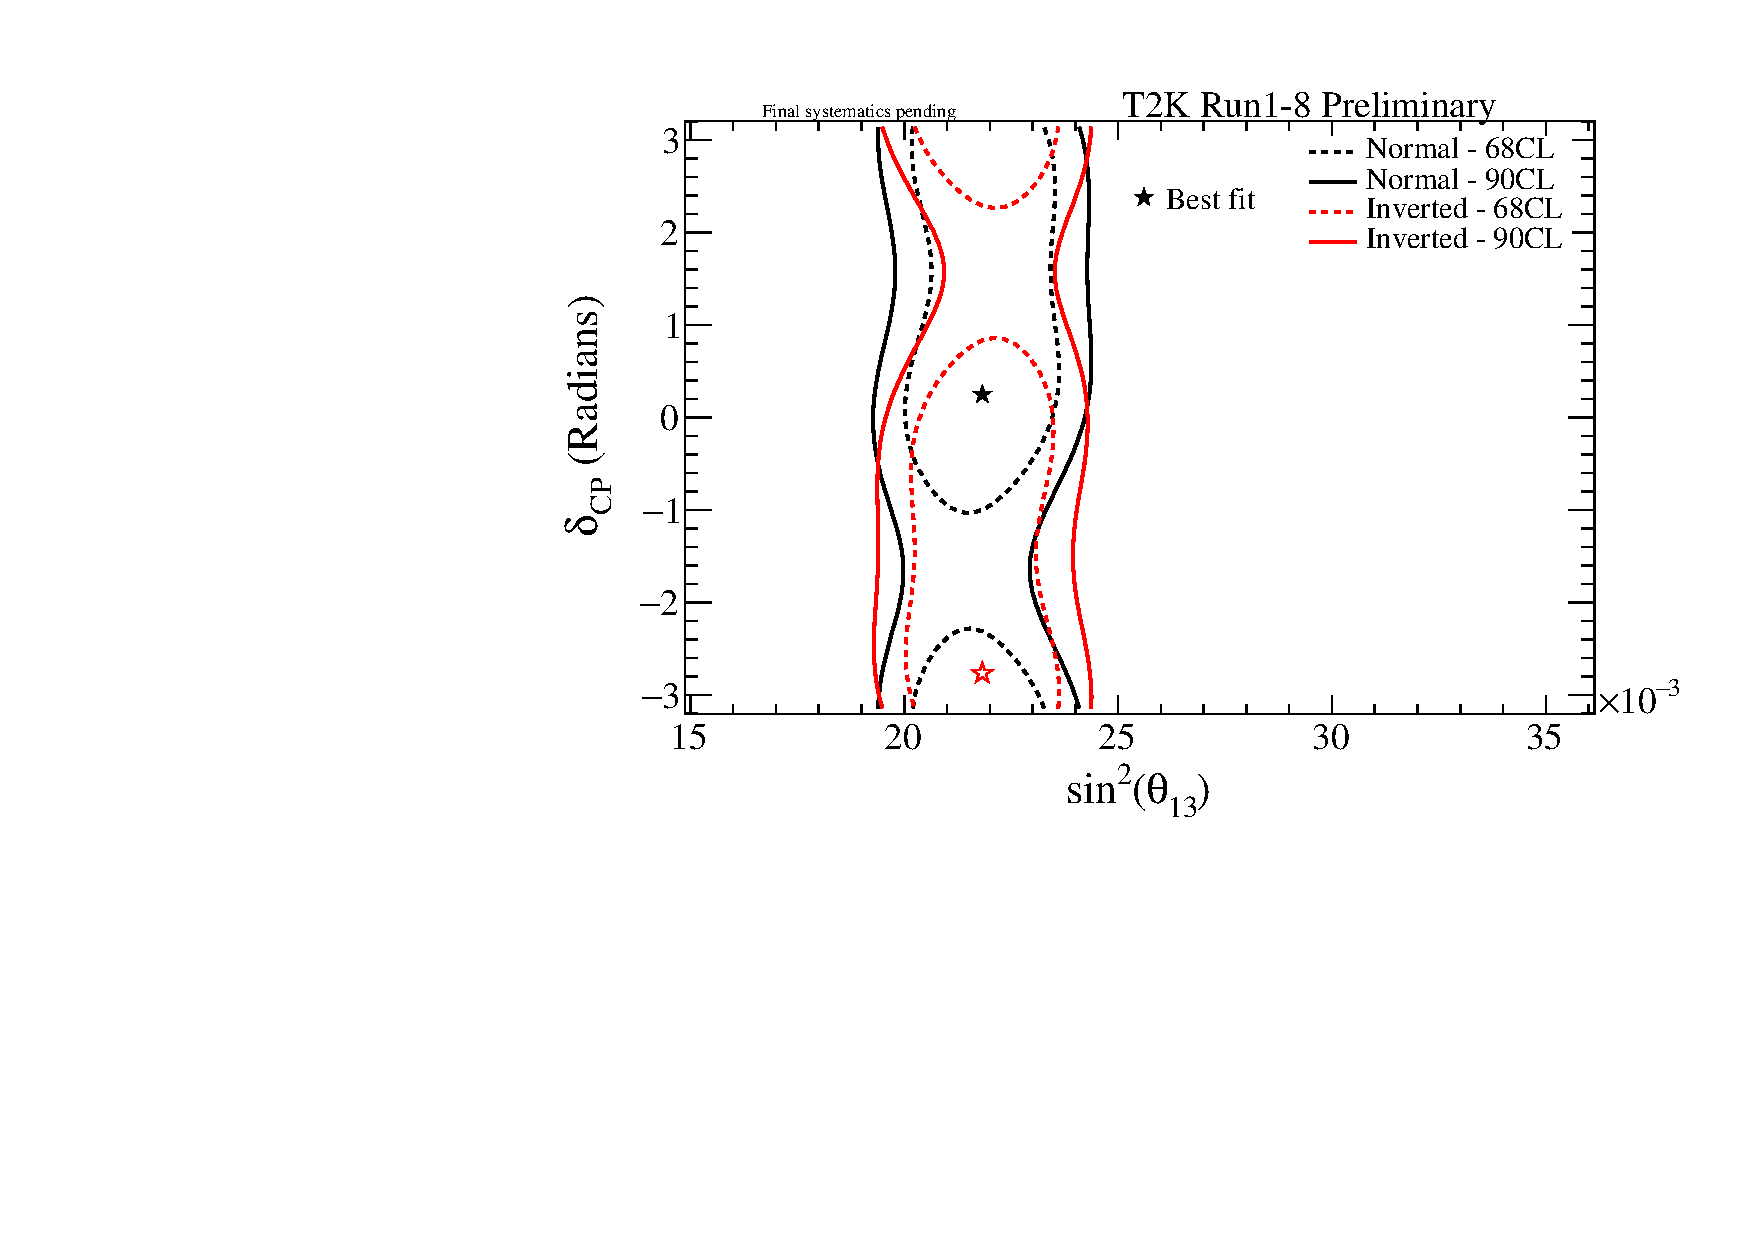
\includegraphics[width=0.9\textwidth]{sensitivity/reactor/mixing13_deltacp_AsimovB_reactor_global}
		\caption{Asimov B \appearance with reactor constraint}
	\end{subfigure}
	\begin{subfigure}[b]{0.49\textwidth}
		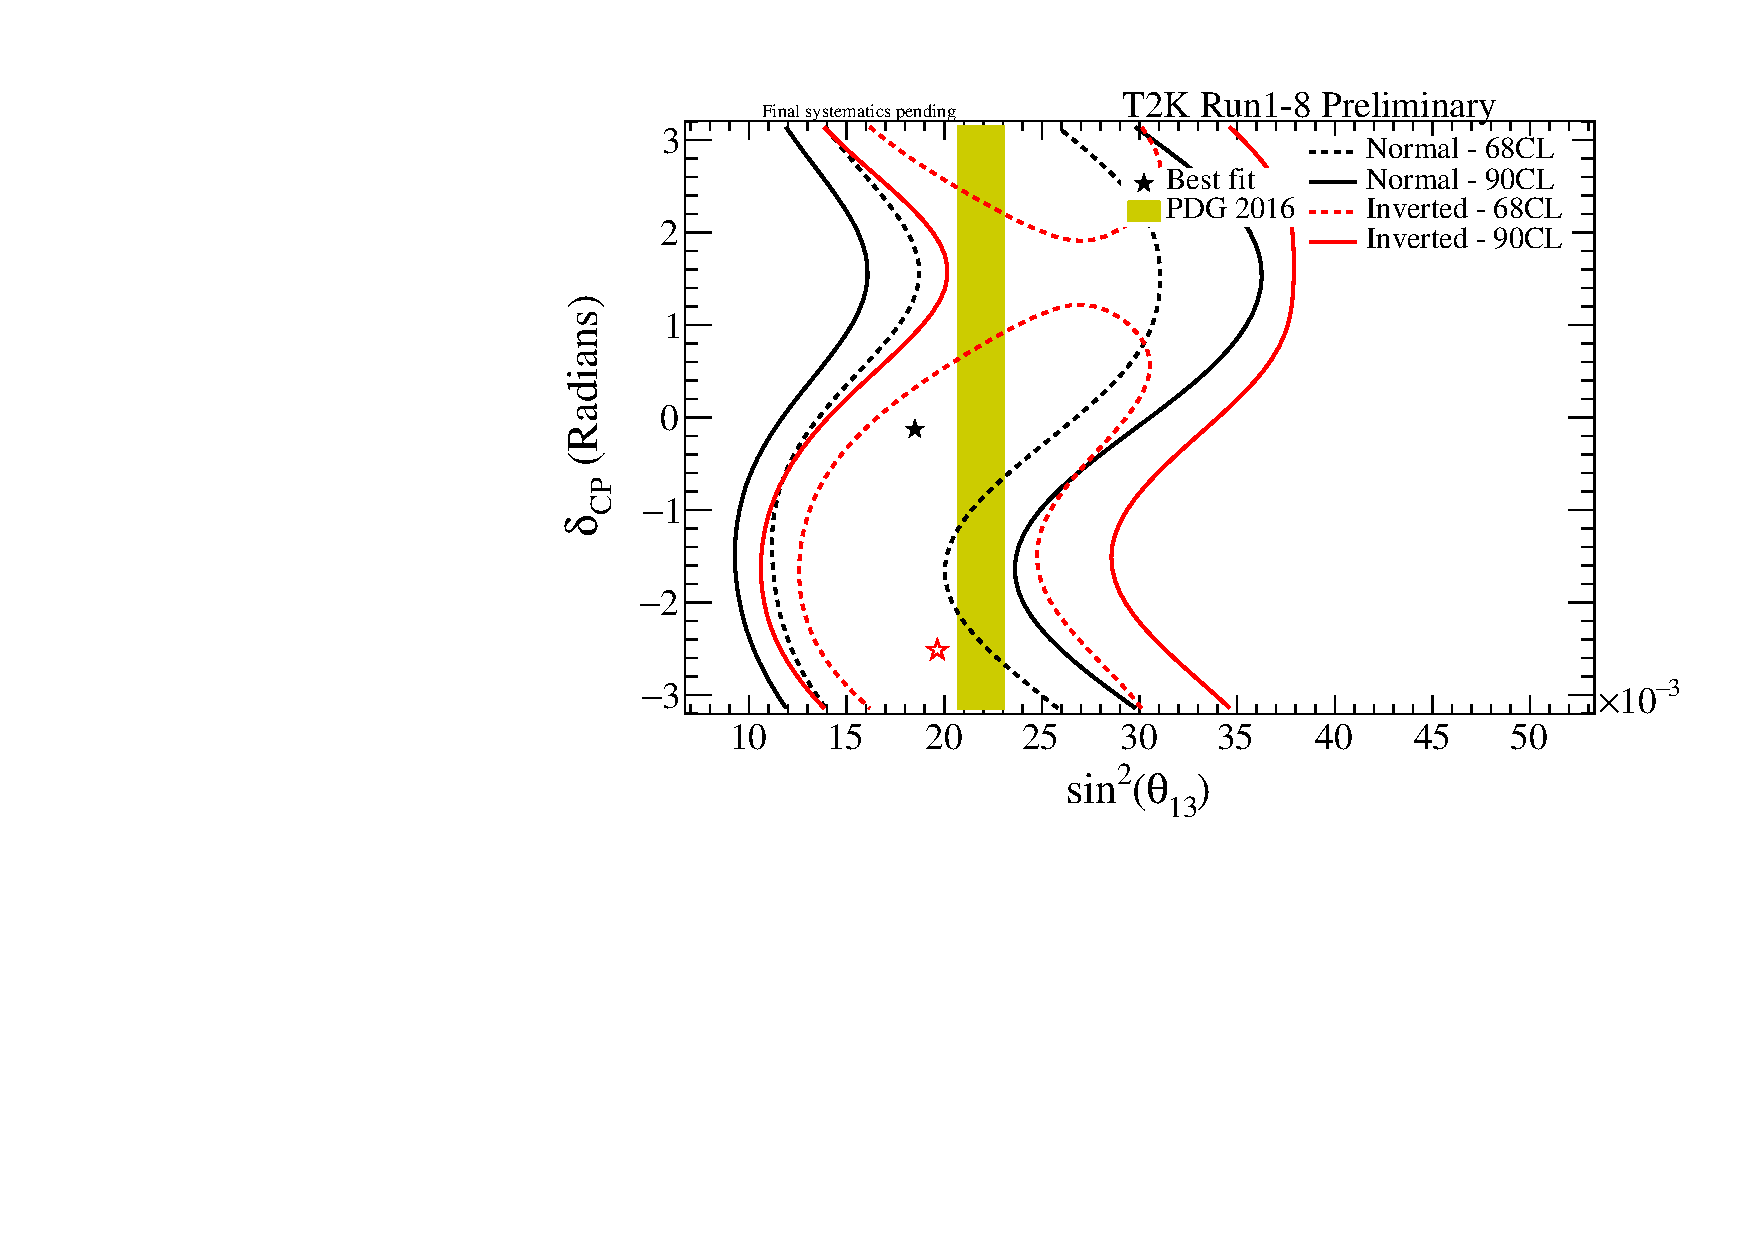
\includegraphics[width=0.9\textwidth]{sensitivity/t2k/mixing13_deltacp_AsimovB_t2k_global}
		\caption{Asimov B \appearance T2K only}
	\end{subfigure}
	\caption {
		Contours at 68\% and 90\% CL for \appearance with and without reactor constraint for Asimov data sets A and B. Normal and inverted hierarchy contours are independent. All 5 samples were used to produce these fits.
	}
	\label{fig:ssqth13_vs_dcp_sensitivity}
\end{figure*}
\clearpage
\subsubsection{Results for \disappearance}

The sensitivity to \disappearance with reactor constraint and T2K only is shown for the Asimov data sets A and B in fig.~\ref{fig:ssqth23_vs_dmsq23_sensitivity}.

\begin{figure*}[htb]
	\center
	\begin{subfigure}[b]{0.49\textwidth}
		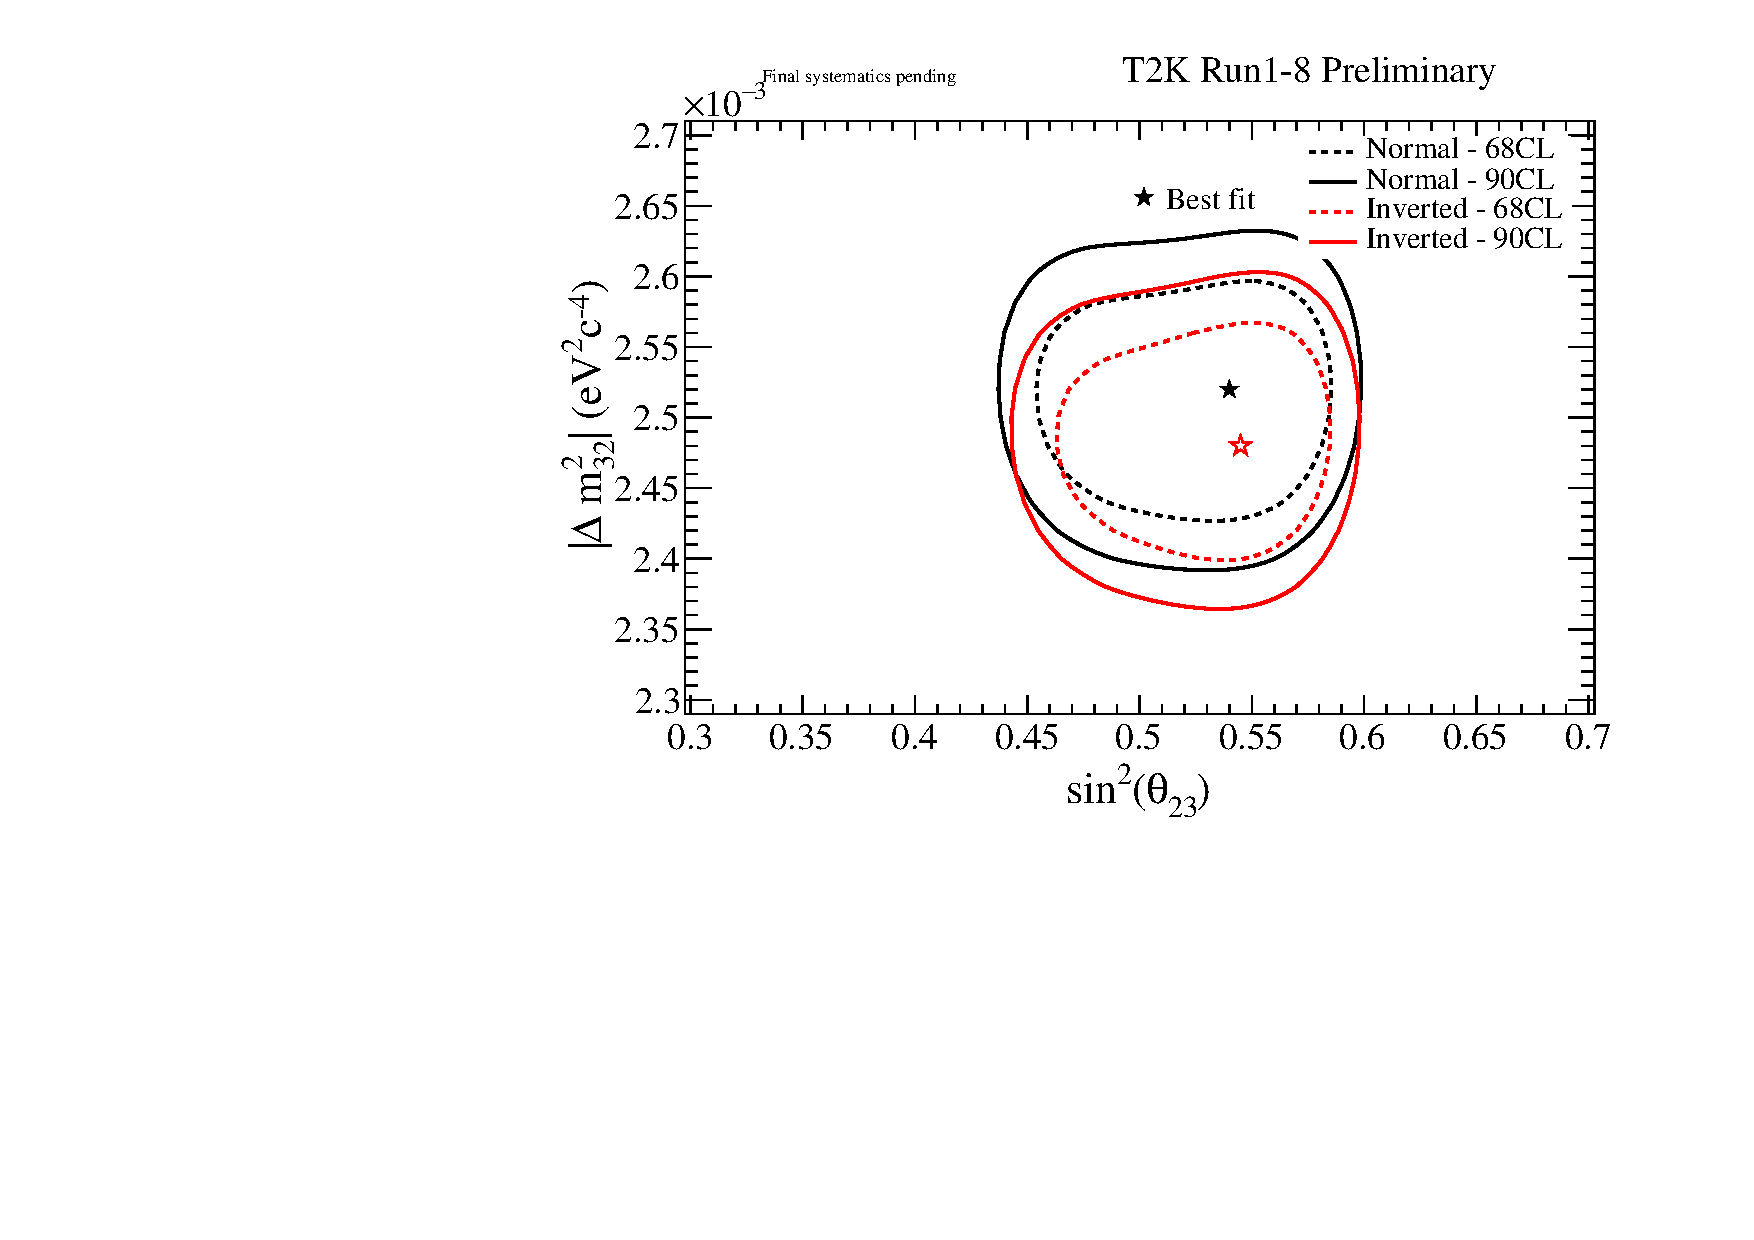
\includegraphics[width=0.9\textwidth]{sensitivity/reactor/mixing23_dmsq23_AsimovA_reactor_global}
		\caption{Asimov A \disappearance with reactor constraint}
	\end{subfigure}
	\begin{subfigure}[b]{0.49\textwidth}
		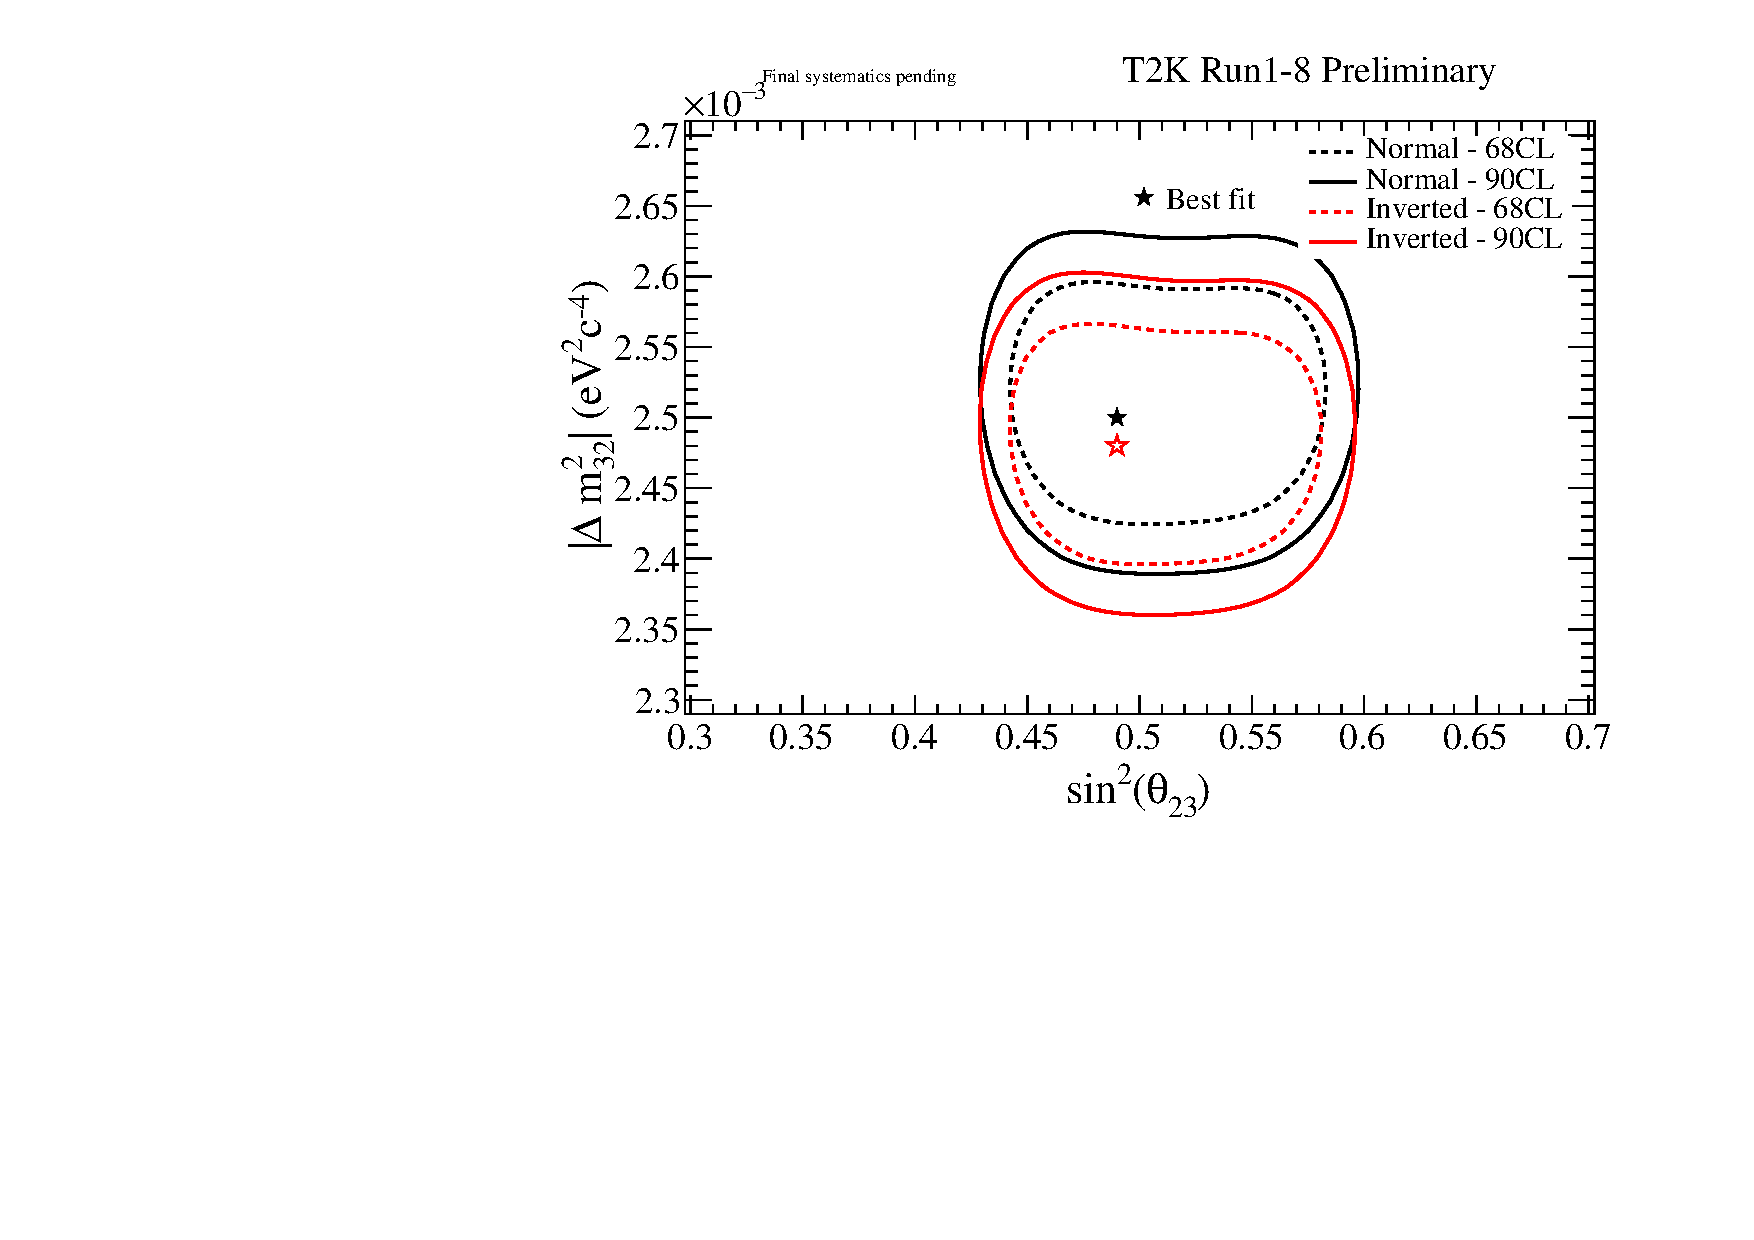
\includegraphics[width=0.9\textwidth]{sensitivity/t2k/mixing23_dmsq23_AsimovA_t2k_global}
		\caption{Asimov A \disappearance T2K only}
	\end{subfigure}
	\begin{subfigure}[b]{0.49\textwidth}
		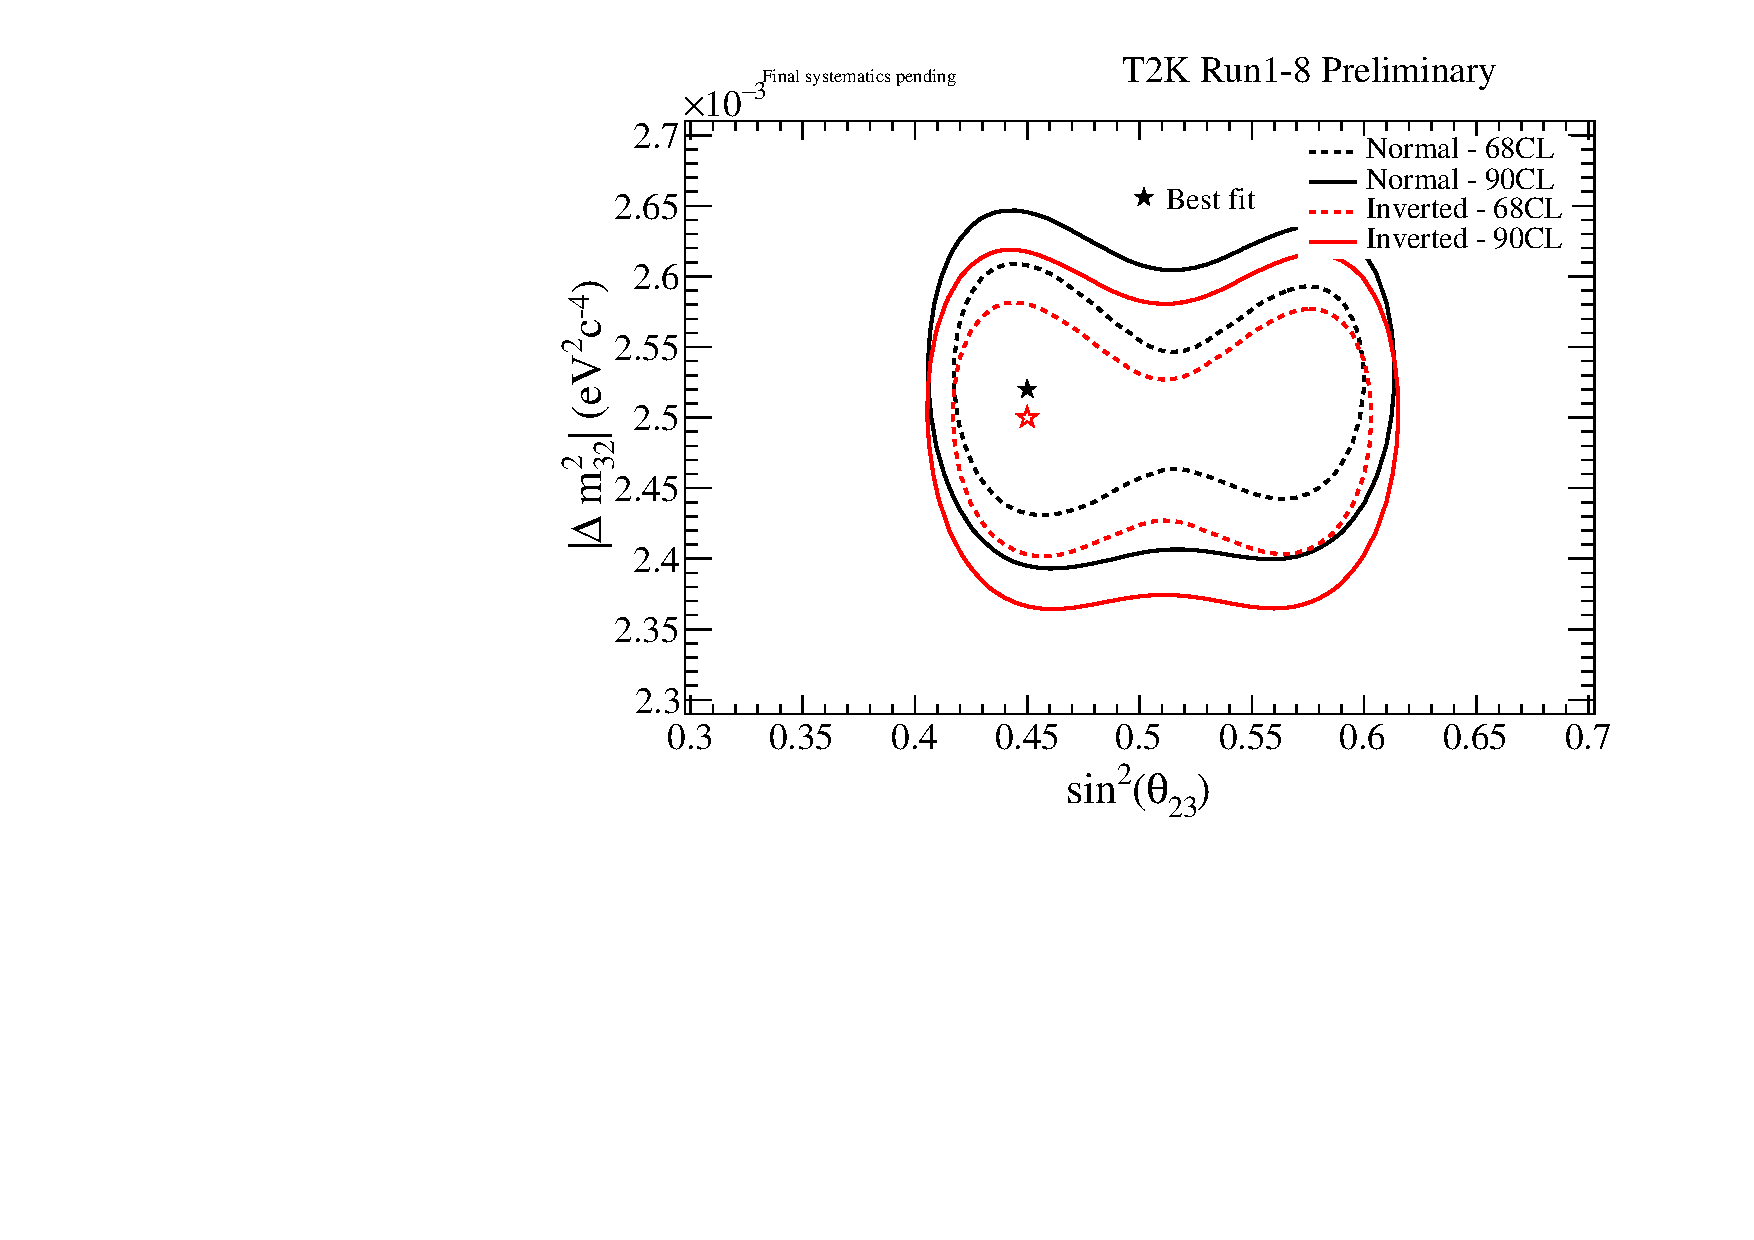
\includegraphics[width=0.9\textwidth]{sensitivity/reactor/mixing23_dmsq23_AsimovB_reactor_global}
		\caption{Asimov B \disappearance with reactor constraint}
	\end{subfigure}
	\begin{subfigure}[b]{0.49\textwidth}
		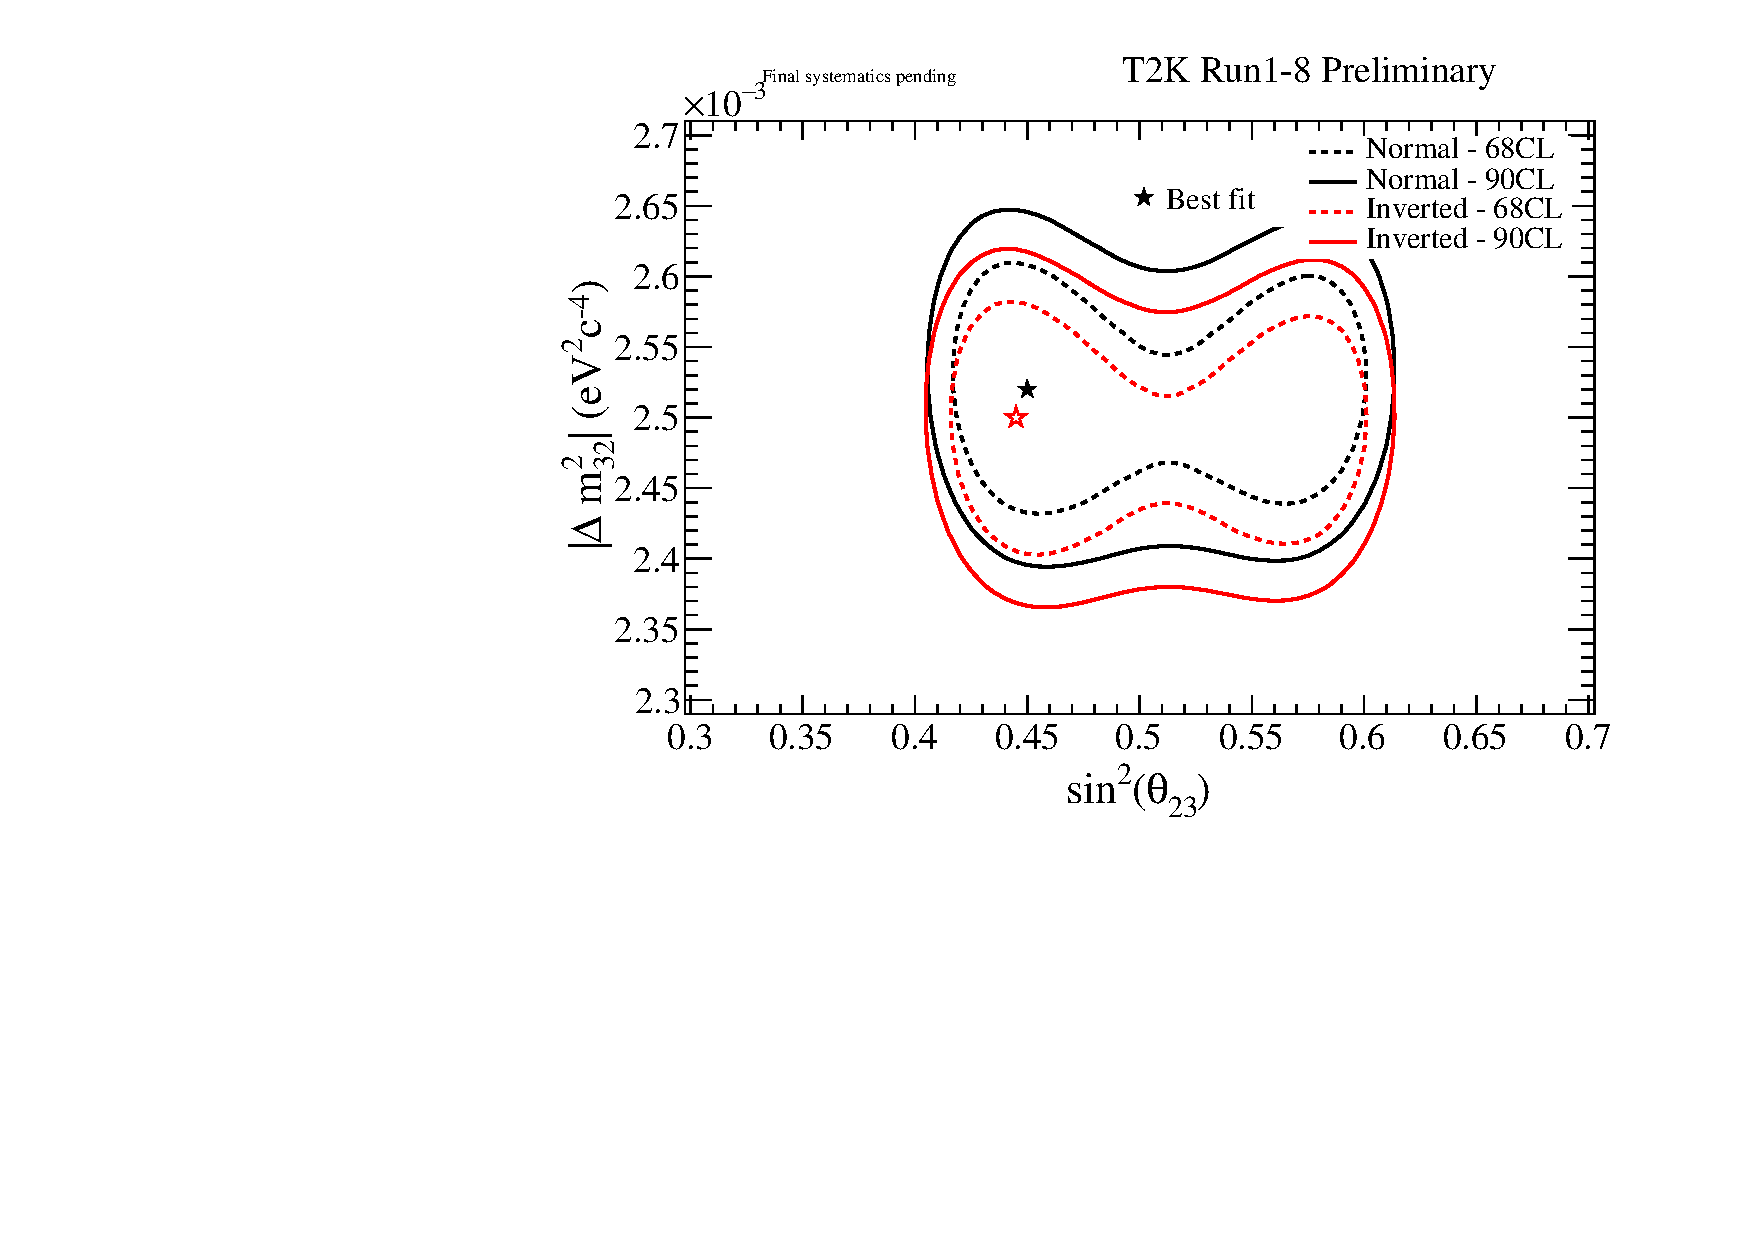
\includegraphics[width=0.9\textwidth]{sensitivity/t2k/mixing23_dmsq23_AsimovB_t2k_global}
		\caption{Asimov B \disappearance T2K only}
	\end{subfigure}
	\caption {
		Contours at 68\% and 90\% CL for \disappearance with and without reactor constraint for Asimov data sets A and B. Normal and inverted hierarchy contours are independent. All 5 samples were used to produce these fits.
	}
	\label{fig:ssqth23_vs_dmsq23_sensitivity}
\end{figure*}
\clearpage
\subsubsection{Results for \deltacp}

The sensitivity to \deltacp with reactor constraint and T2K only is shown for the Asimov data sets A and B in fig.~\ref{fig:dcp_sensitivity}.

\begin{figure*}[htb]
	\center
	\begin{subfigure}[b]{0.49\textwidth}
		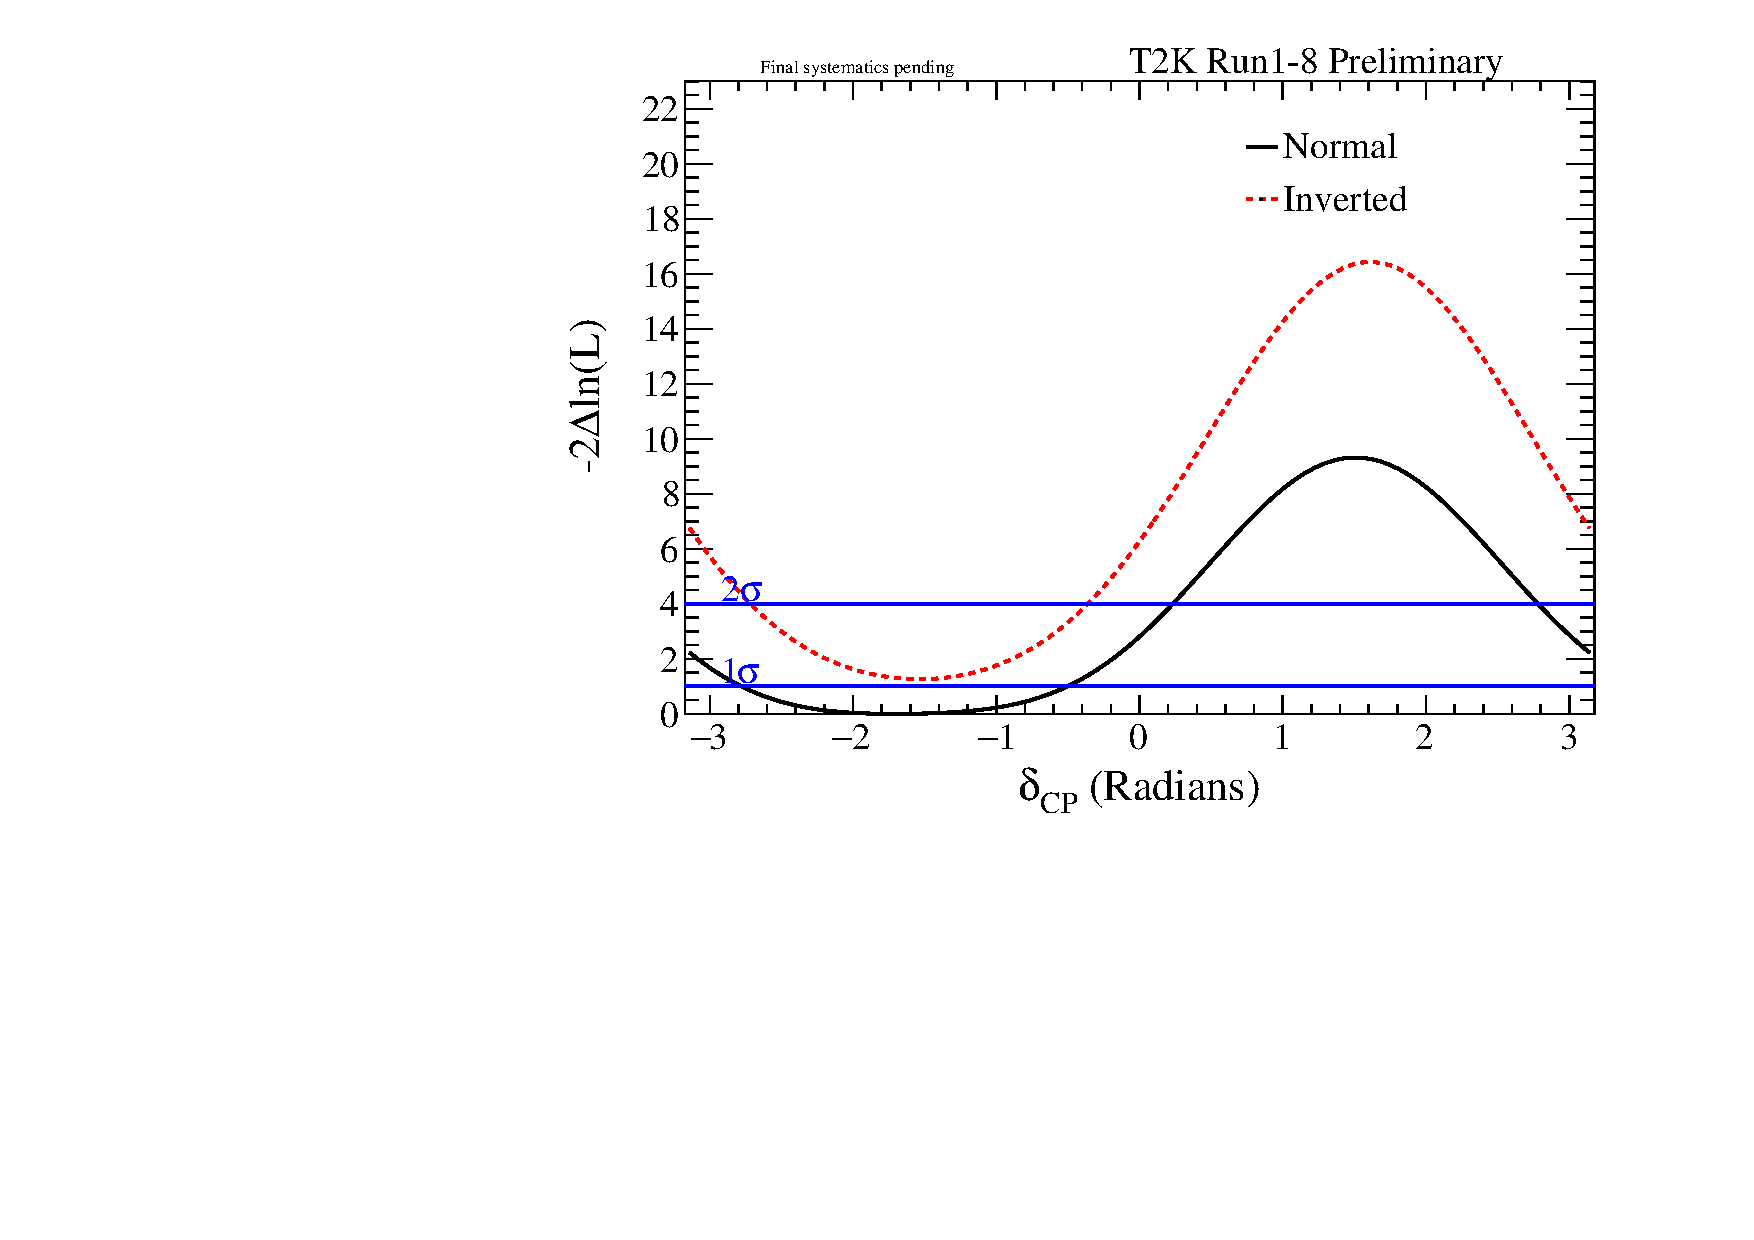
\includegraphics[width=0.9\textwidth]{sensitivity/reactor/deltacp_AsimovA_reactor_global}
		\caption{Asimov A \deltacp with reactor constraint}
	\end{subfigure}
	\begin{subfigure}[b]{0.49\textwidth}
		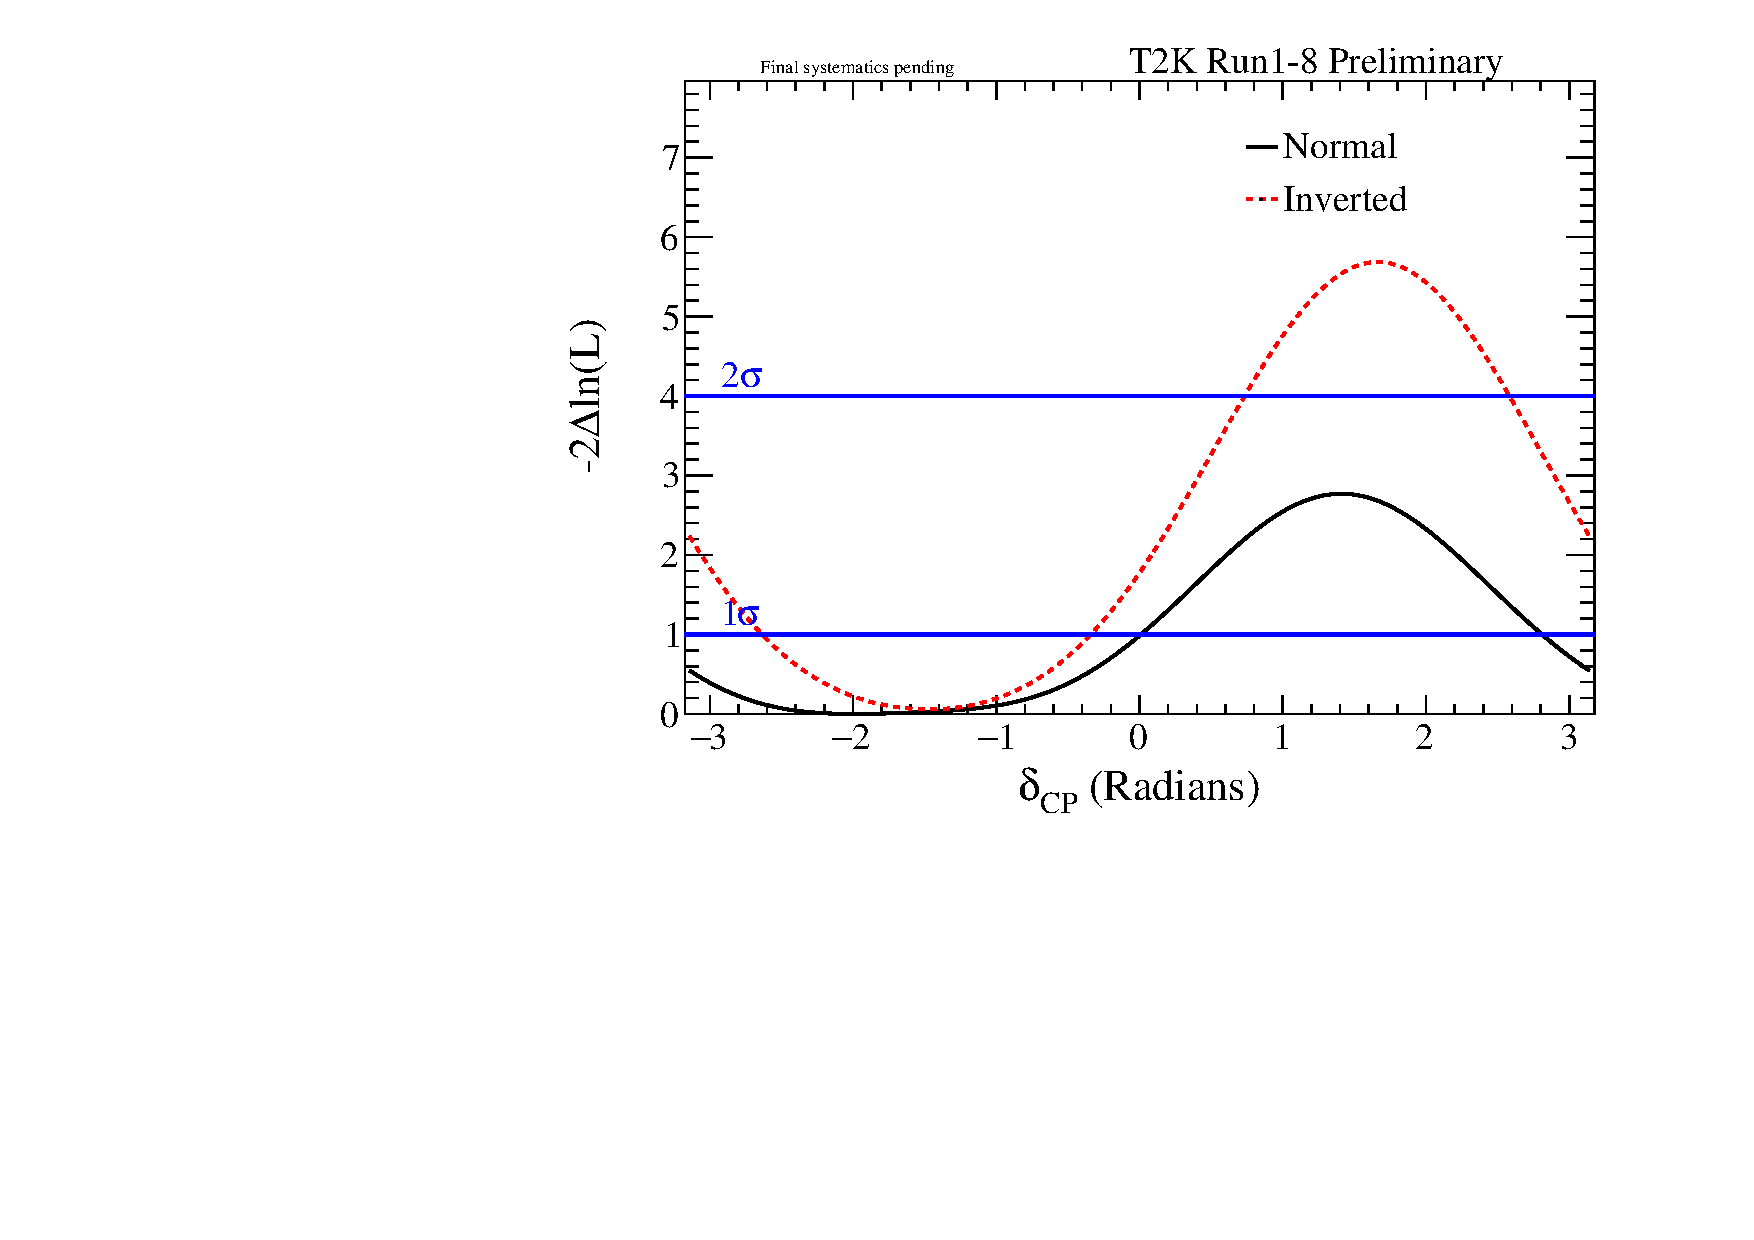
\includegraphics[width=0.9\textwidth]{sensitivity/t2k/deltacp_AsimovA_t2k_global}
		\caption{Asimov A \deltacp T2K only}
	\end{subfigure}
	\begin{subfigure}[b]{0.49\textwidth}
		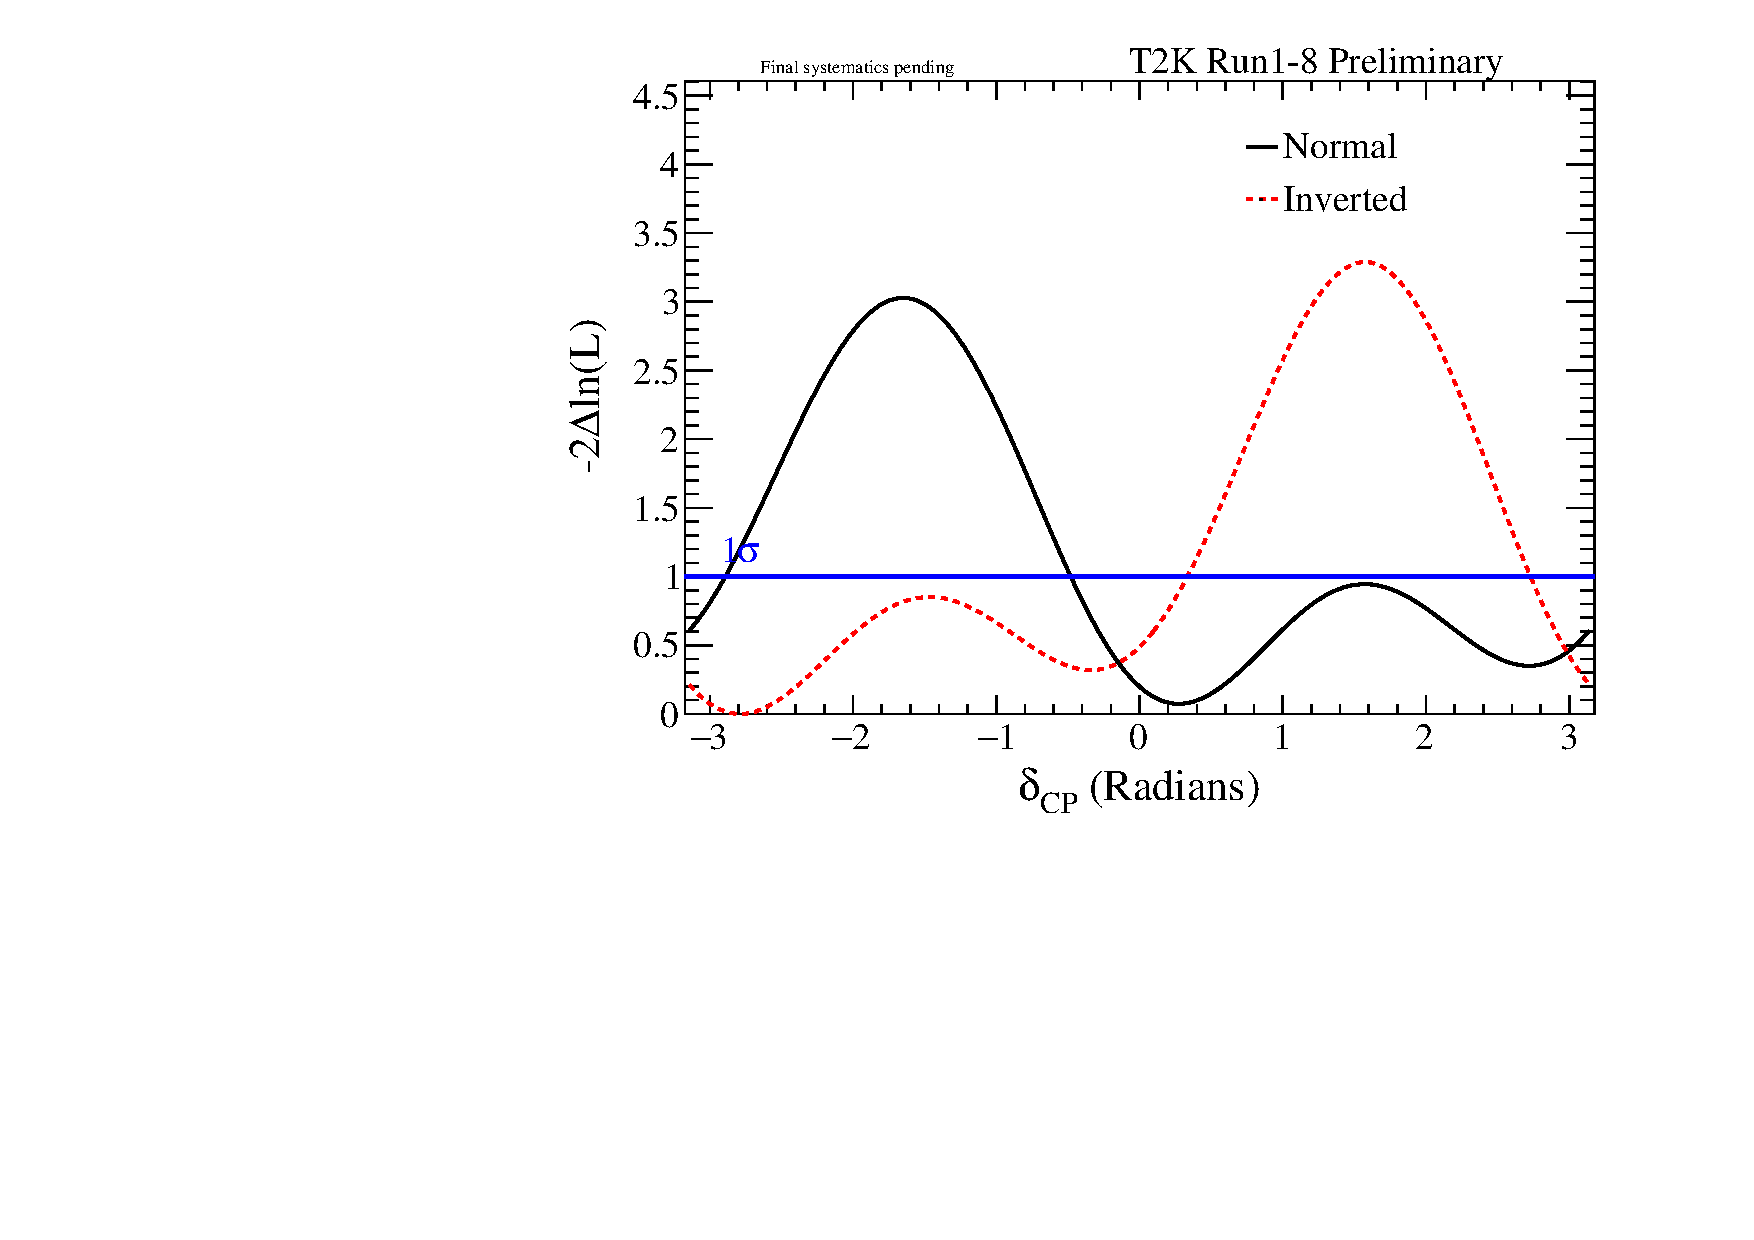
\includegraphics[width=0.9\textwidth]{sensitivity/reactor/deltacp_AsimovB_reactor_global}
		\caption{Asimov B \deltacp with reactor constraint}
	\end{subfigure}
	\begin{subfigure}[b]{0.49\textwidth}
		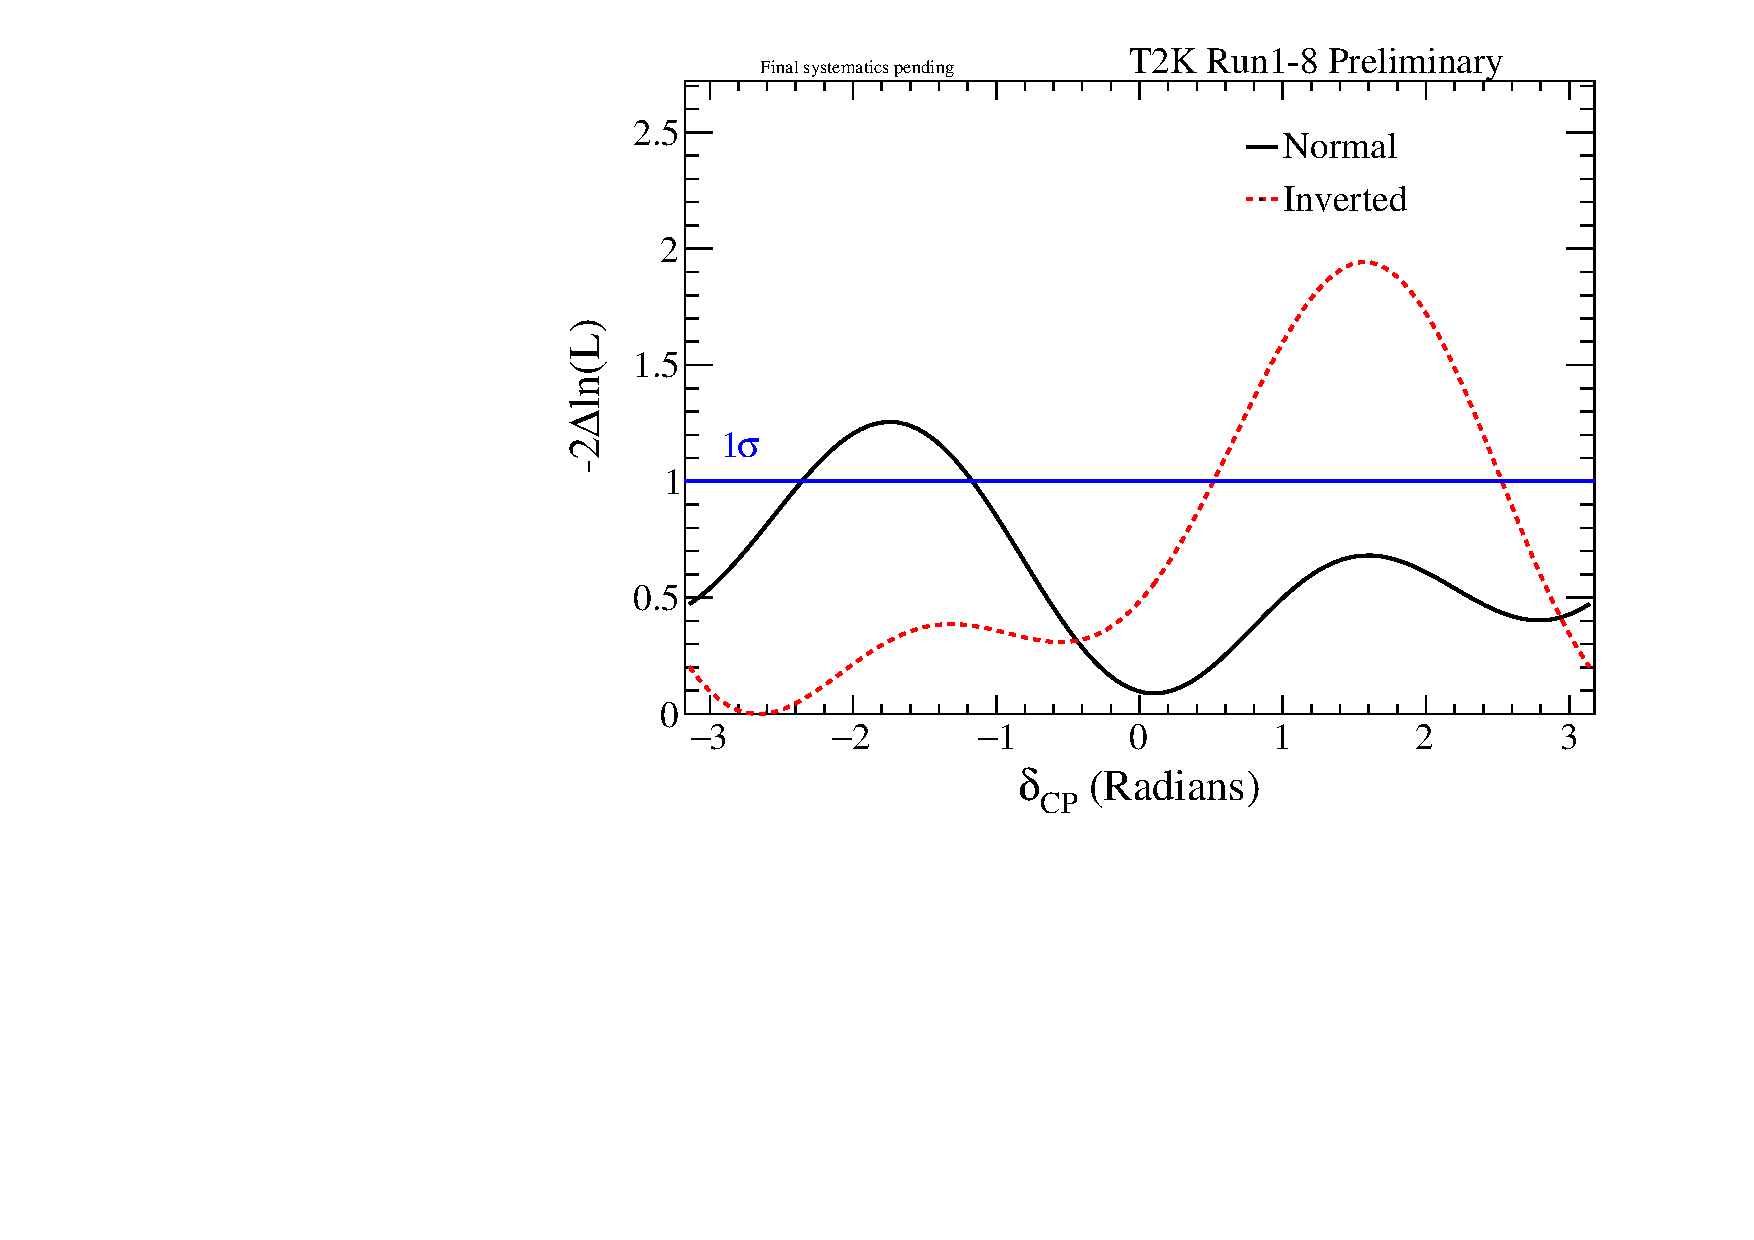
\includegraphics[width=0.9\textwidth]{sensitivity/t2k/deltacp_AsimovB_t2k_global}
		\caption{Asimov B \deltacp T2K only}
	\end{subfigure}
	\caption {
		The expected $\Delta\chi^2$ distribution as a function of \deltacp with and without reactor constraint for Asimov data sets A and B. The mass hierarchy is minimized, with normal and inverted hierarchy $\Delta\chi^2$ distributions shifted to the same global best-fit $\chi^2$ value, which is taken to be the minimum between normal and inverted hierarchy. All 5 samples were used to produce these fits.
	}
	\label{fig:dcp_sensitivity}
\end{figure*}
\clearpage
\subsubsection{Results for \ssqthonethree}

The sensitivity to \ssqthonethree (without reactor constraint) is shown for the Asimov data sets A and B in fig.~\ref{fig:th13_sensitivity}.

\begin{figure*}[htb]
	\center
	\begin{subfigure}[b]{0.49\textwidth}
		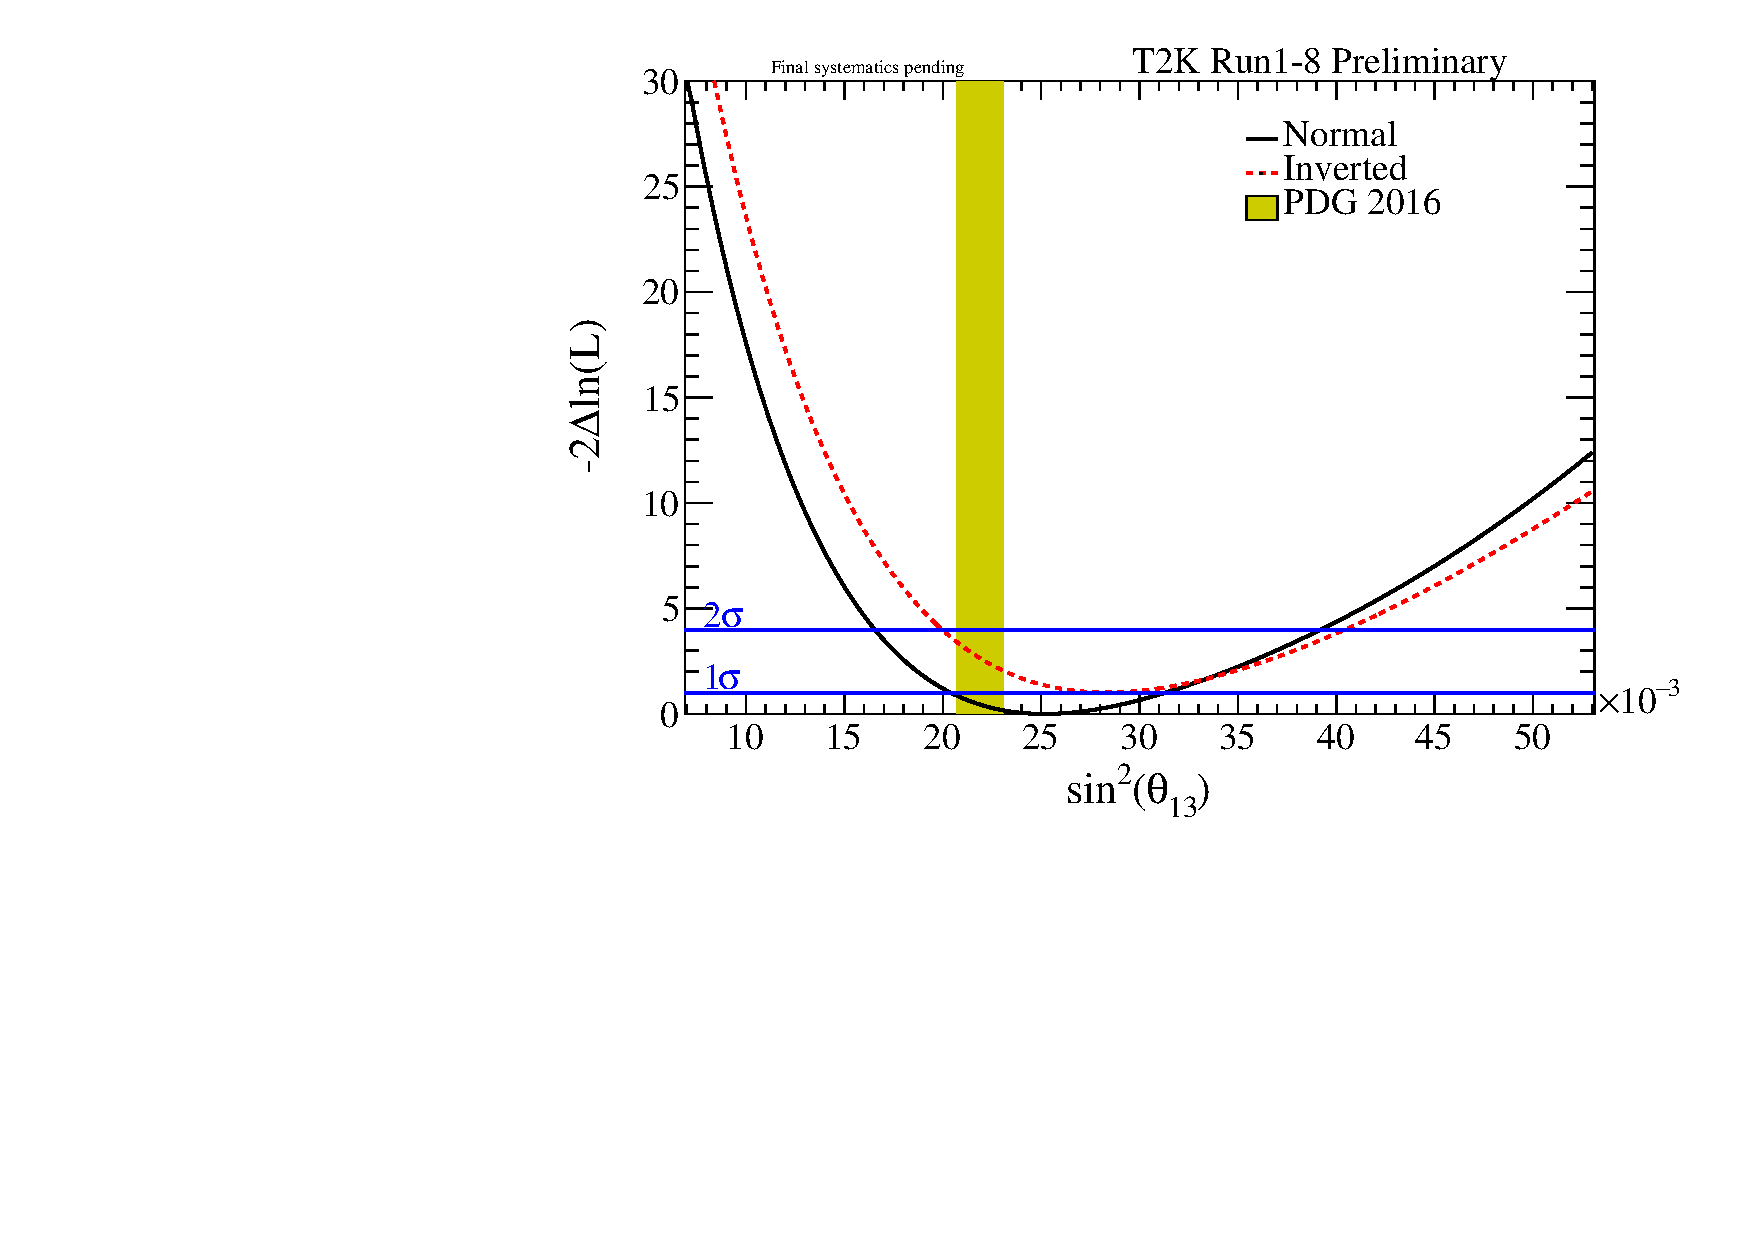
\includegraphics[width=0.9\textwidth]{sensitivity/t2k/mixing13_AsimovA_t2k_global}
		\caption{Asimov A \ssqthonethree T2K only}
	\end{subfigure}
	\begin{subfigure}[b]{0.49\textwidth}
		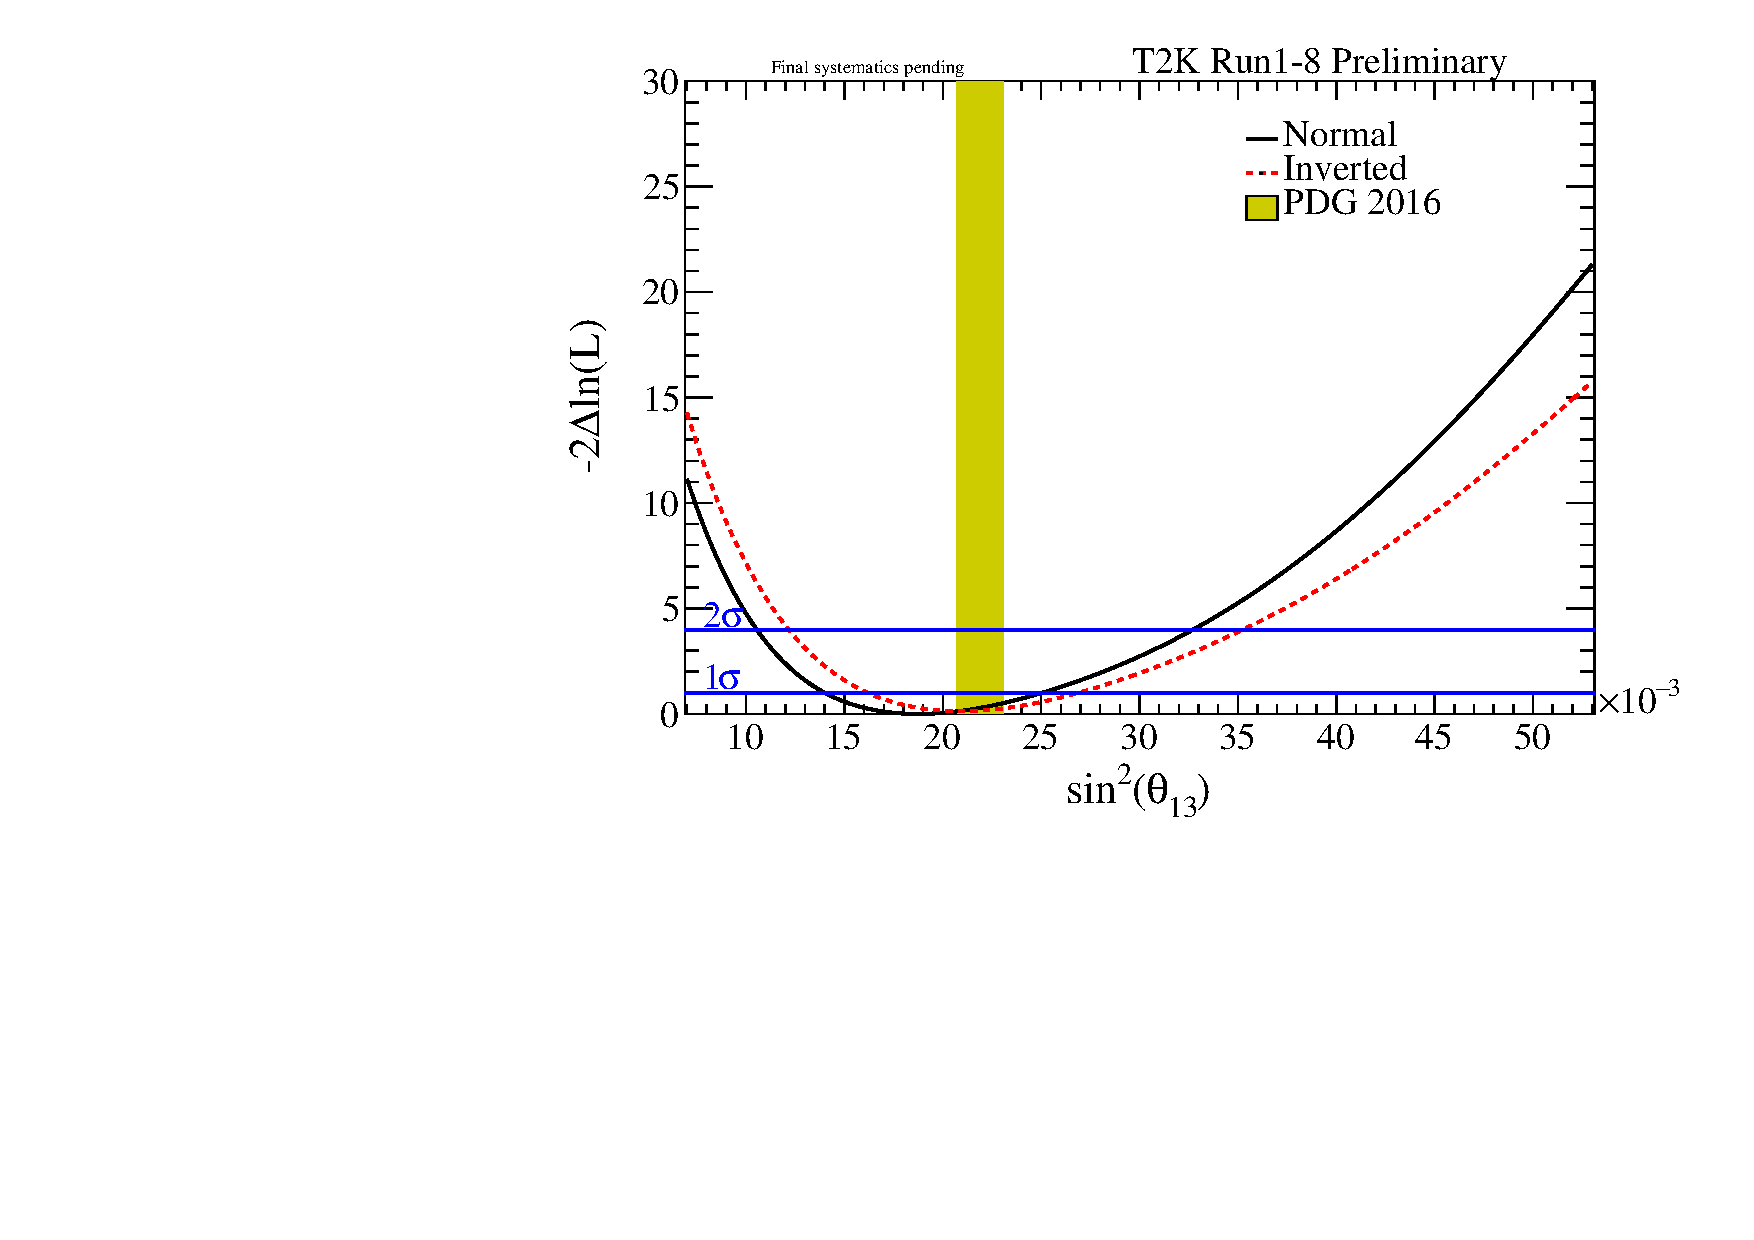
\includegraphics[width=0.9\textwidth]{sensitivity/t2k/mixing13_AsimovB_t2k_global}
		\caption{Asimov B \ssqthonethree T2K only}
	\end{subfigure}
	\caption {
		The expected $\Delta\chi^2$ distribution as a function of \ssqthonethree without reactor constraint for Asimov data sets A and B. The mass hierarchy is minimized, with normal and inverted hierarchy $\Delta\chi^2$ distributions shifted to the same global best-fit $\chi^2$ value, which is taken to be the minimum between normal and inverted hierarchy. All 5 samples were used to produce these fits.
	}
	\label{fig:th13_sensitivity}
\end{figure*}
\clearpage
\subsubsection{Results for \ssqthtwothree}

The sensitivity to \ssqthtwothree with reactor constraint and T2K only is shown for the Asimov data sets A and B in fig.~\ref{fig:th23_sensitivity}.

\begin{figure*}[htb]
	\center
	\begin{subfigure}[b]{0.49\textwidth}
		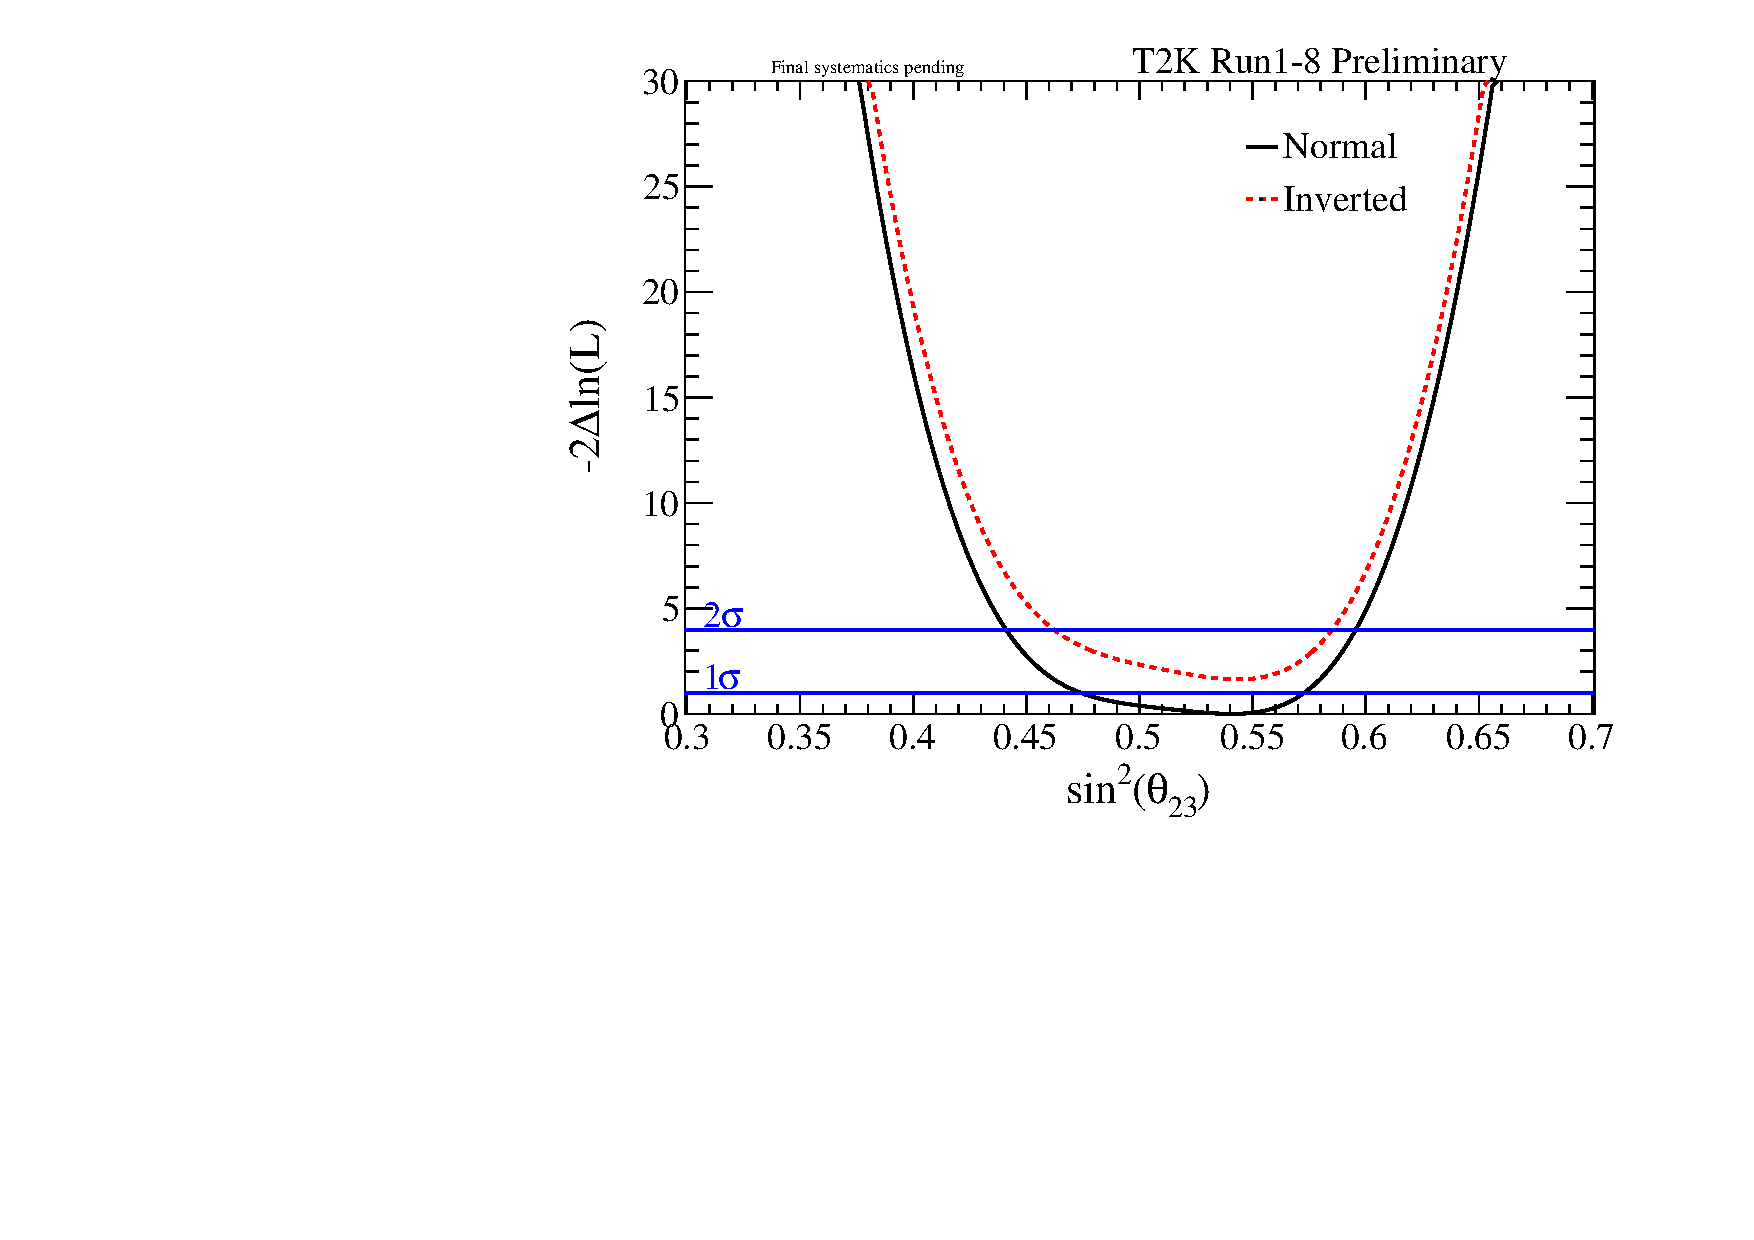
\includegraphics[width=0.9\textwidth]{sensitivity/reactor/mixing23_AsimovA_reactor_global}
		\caption{Asimov A \ssqthtwothree with reactor constraint}
	\end{subfigure}
	\begin{subfigure}[b]{0.49\textwidth}
		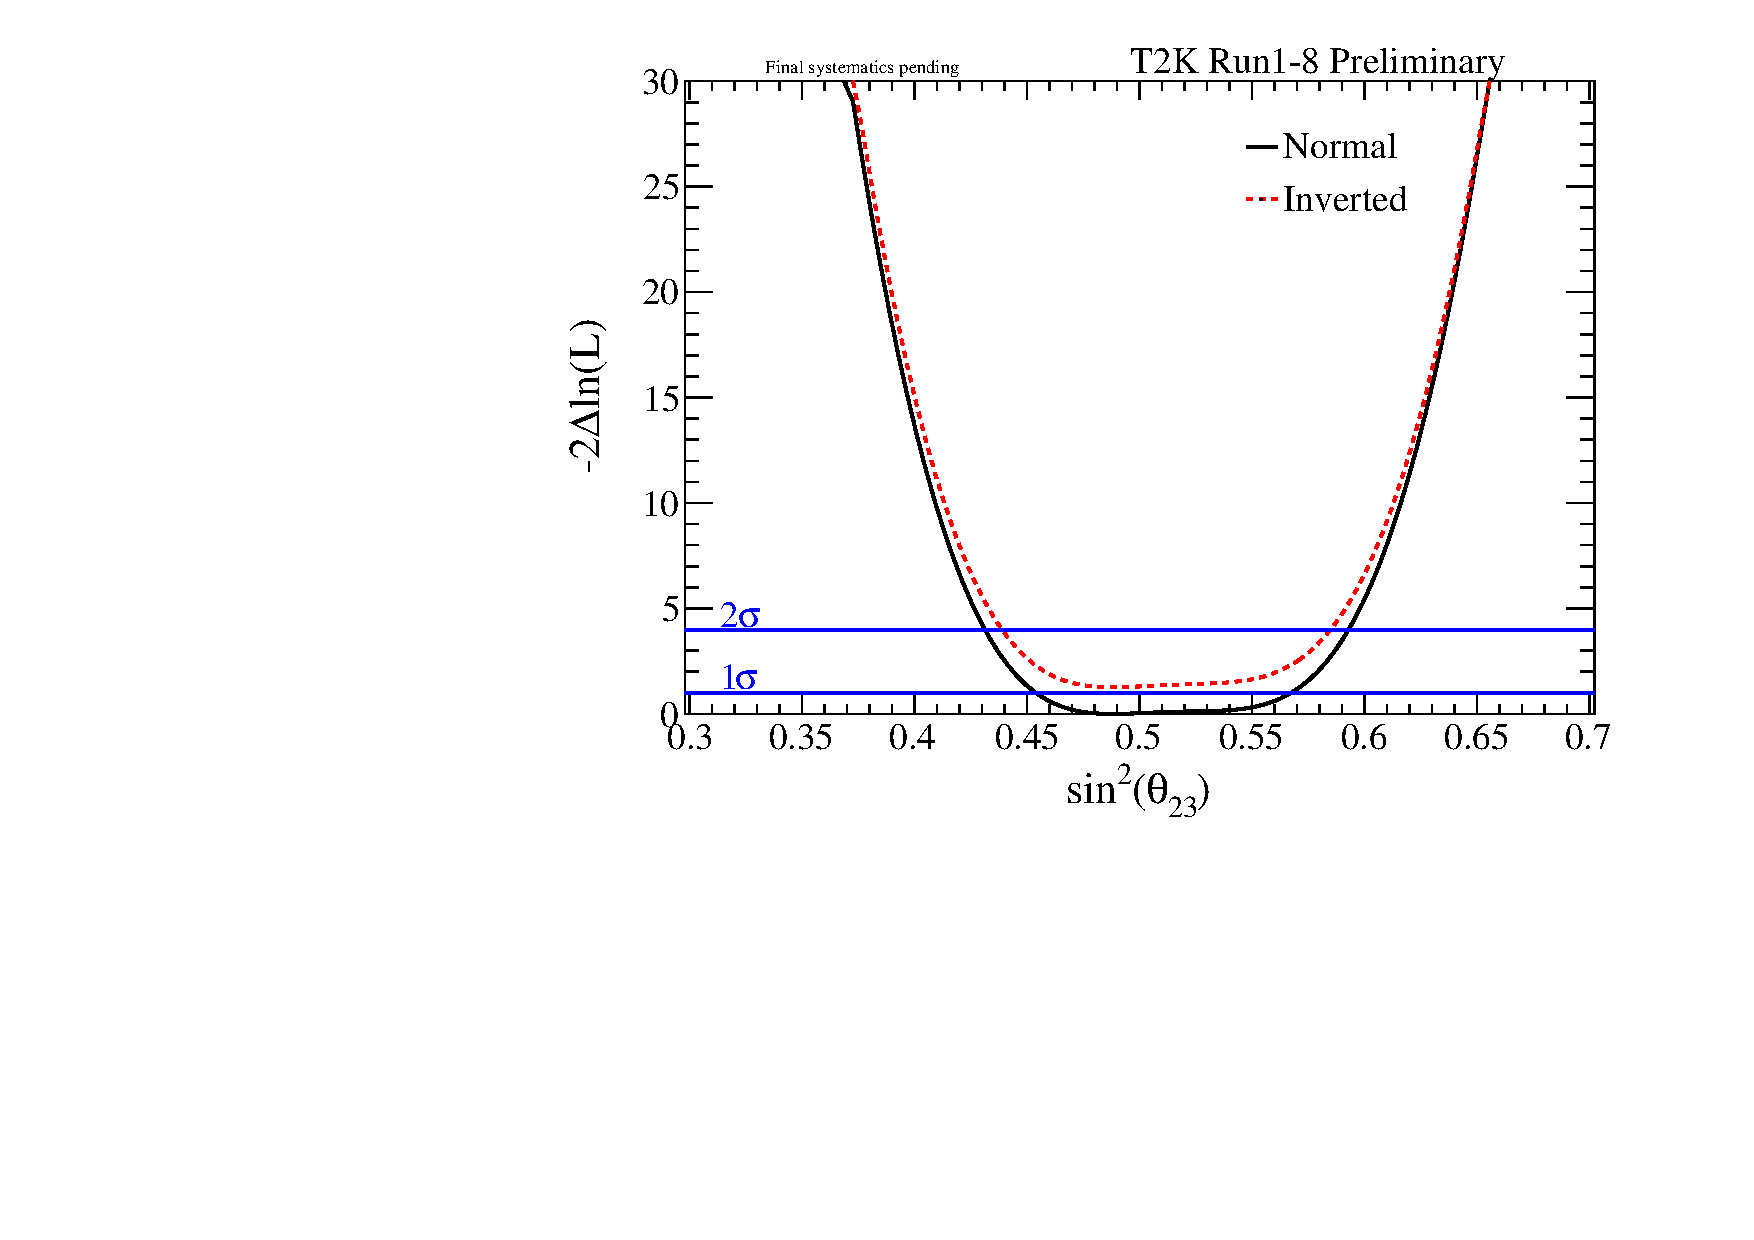
\includegraphics[width=0.9\textwidth]{sensitivity/t2k/mixing23_AsimovA_t2k_global}
		\caption{Asimov A \ssqthtwothree T2K only}
	\end{subfigure}
	\begin{subfigure}[b]{0.49\textwidth}
		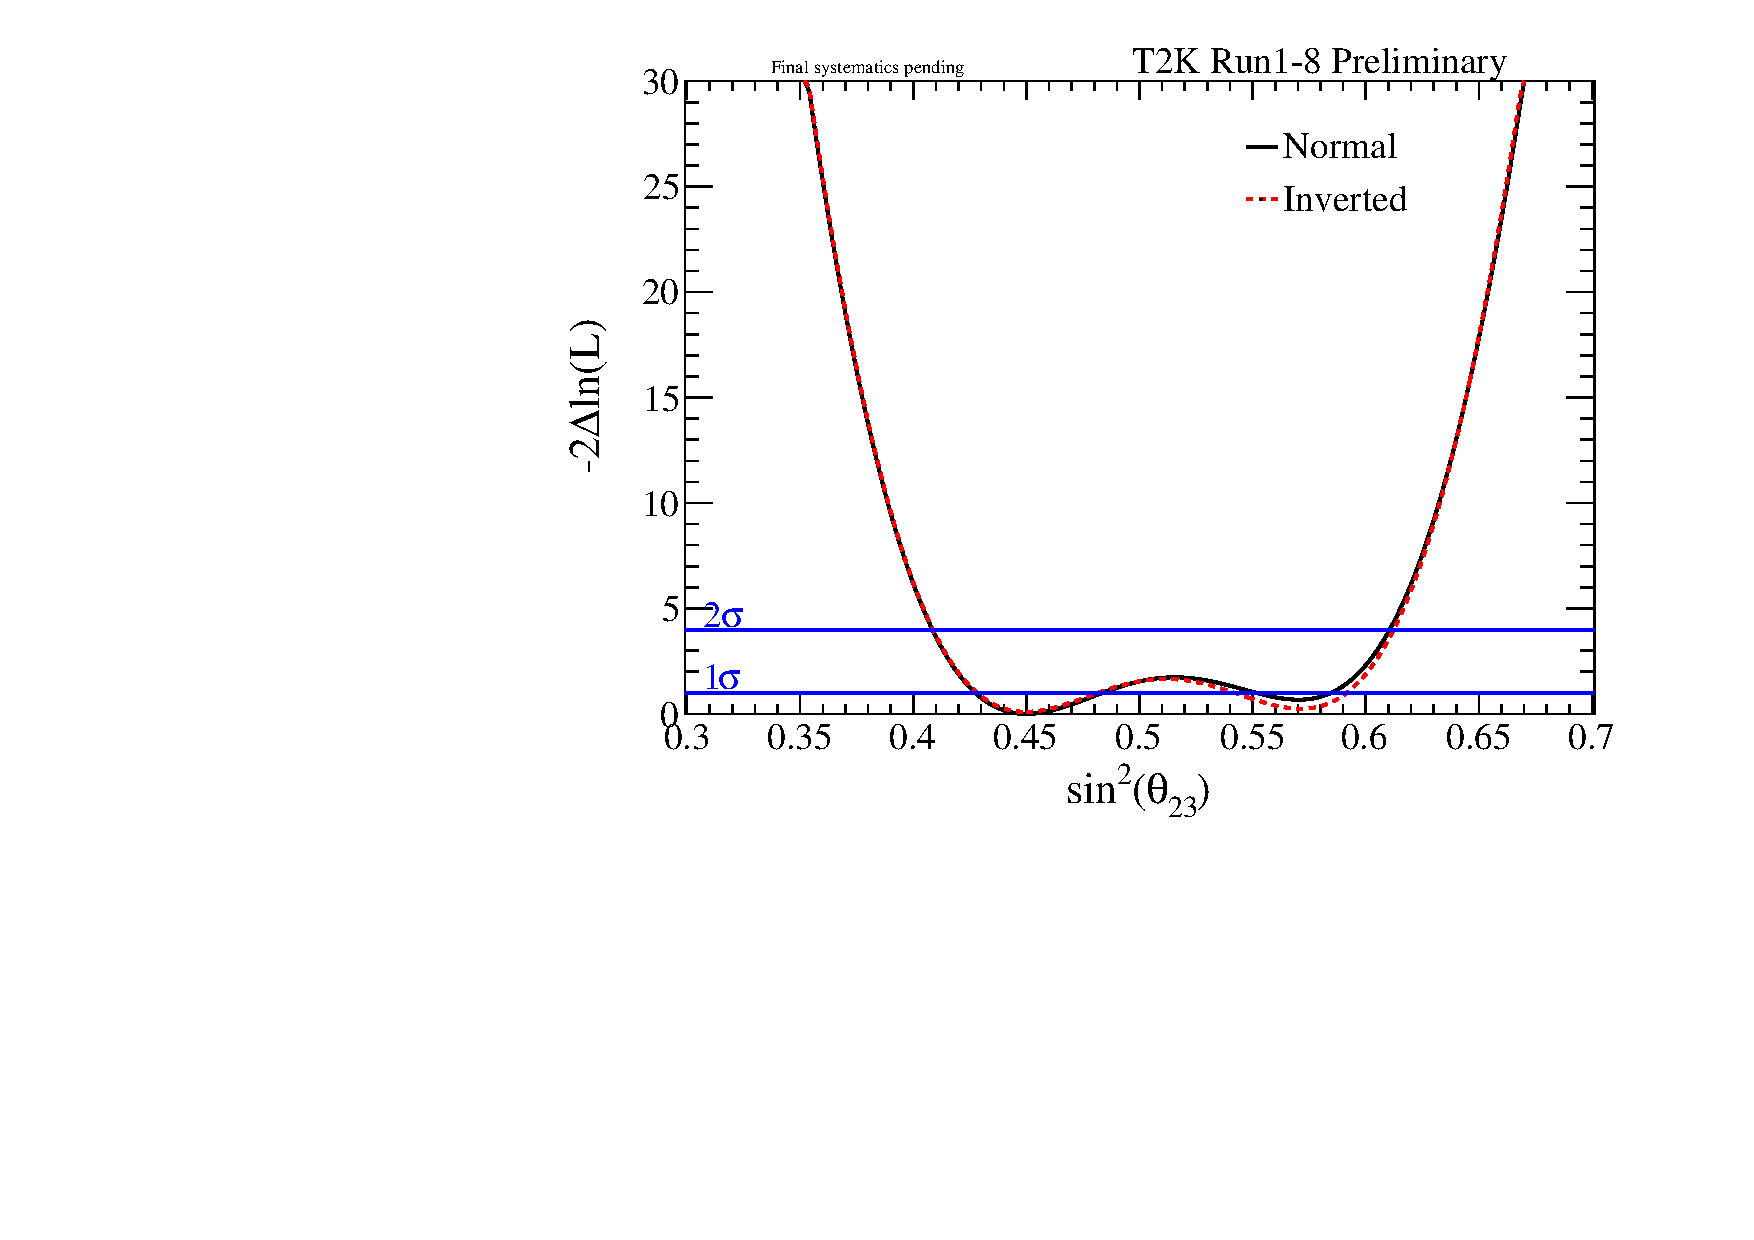
\includegraphics[width=0.9\textwidth]{sensitivity/reactor/mixing23_AsimovB_reactor_global}
		\caption{Asimov B \ssqthtwothree with reactor constraint}
	\end{subfigure}
	\begin{subfigure}[b]{0.49\textwidth}
		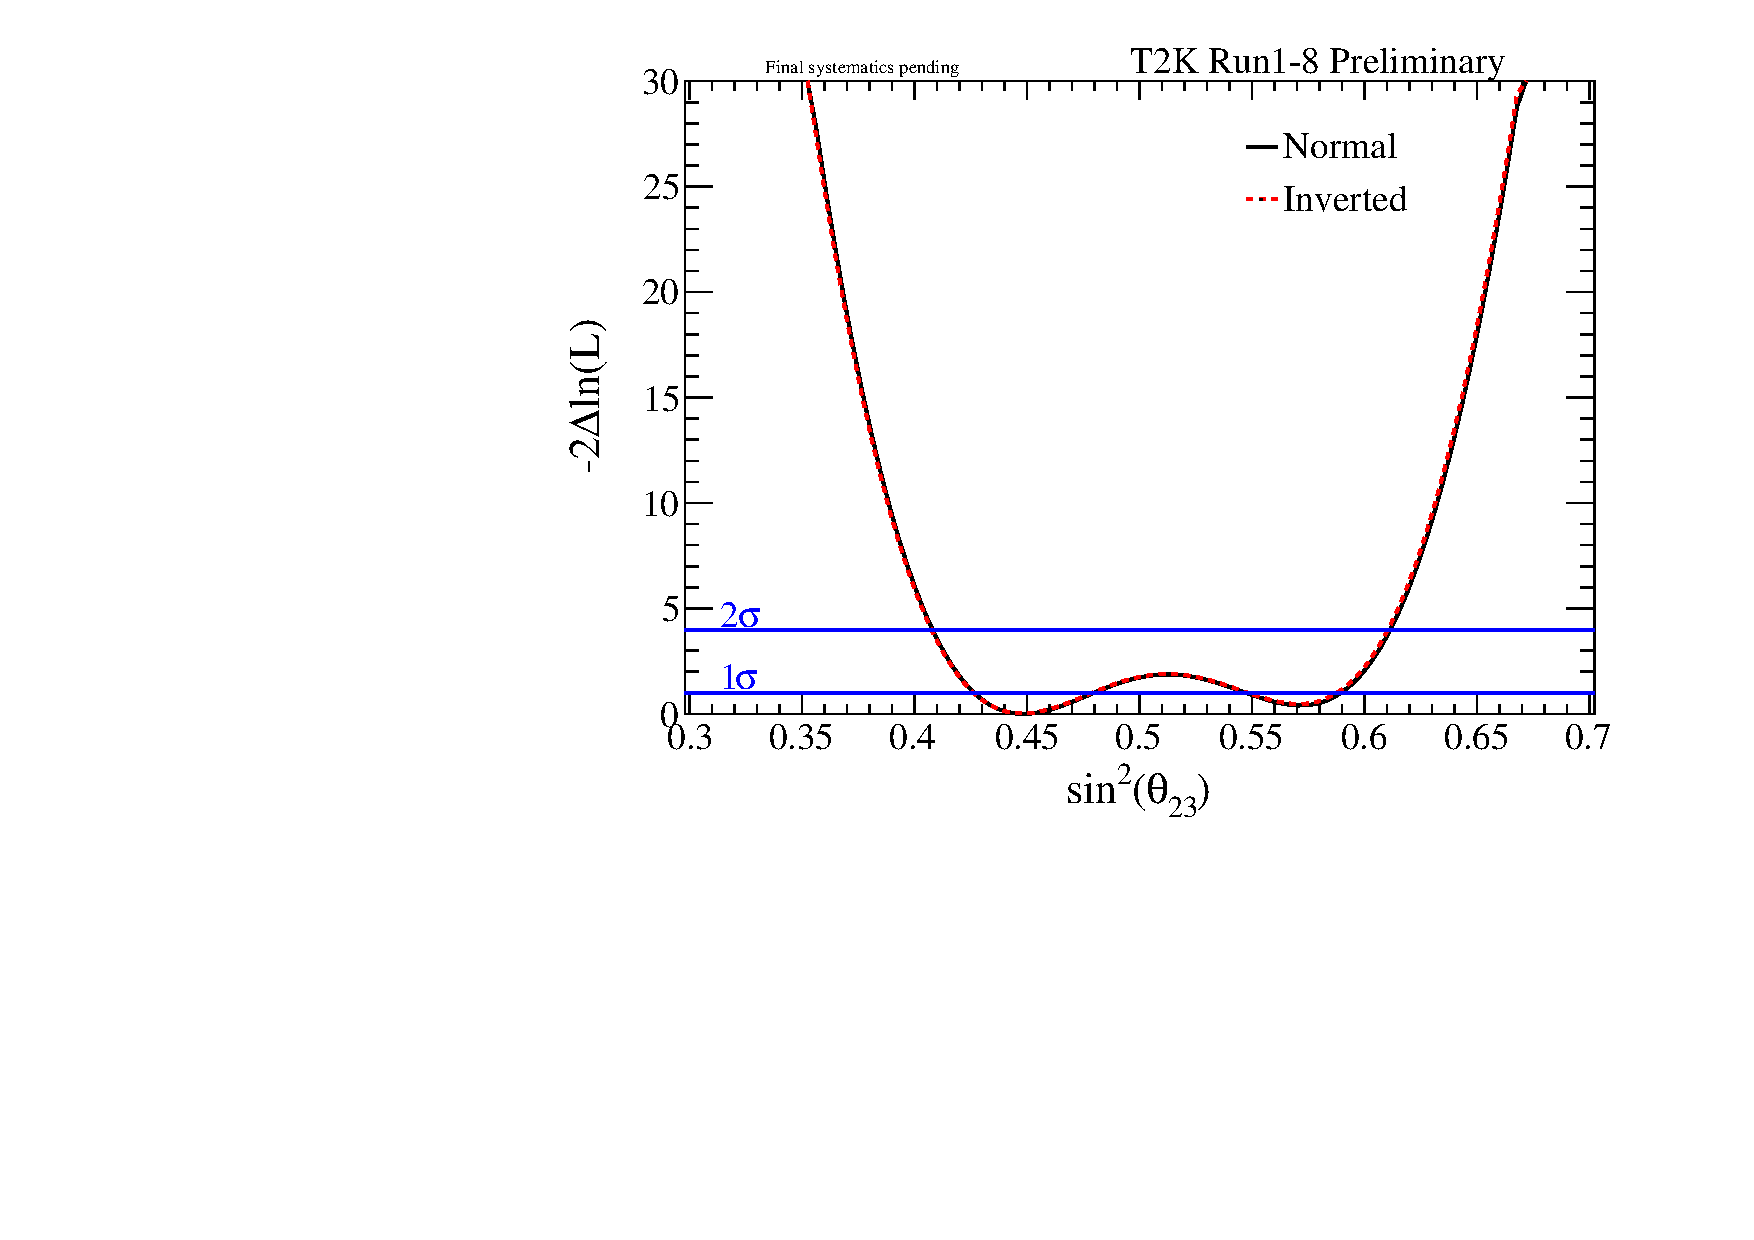
\includegraphics[width=0.9\textwidth]{sensitivity/t2k/mixing23_AsimovB_t2k_global}
		\caption{Asimov B \ssqthtwothree T2K only}
	\end{subfigure}
	\caption {
		The expected $\Delta\chi^2$ distribution as a function of \ssqthtwothree with and without reactor constraint for Asimov data sets A and B. The mass hierarchy is minimized, with normal and inverted hierarchy $\Delta\chi^2$ distributions shifted to the same global best-fit $\chi^2$ value, which is taken to be the minimum between normal and inverted hierarchy. All 5 samples were used to produce these fits.
	}
	\label{fig:th23_sensitivity}
\end{figure*}
\clearpage
\subsubsection{Results for \dmsqtwothree}

The sensitivity to \dmsqtwothree with reactor constraint and T2K only is shown for the Asimov data sets A and B in fig.~\ref{fig:dmsq23_sensitivity}.

\begin{figure*}[htb]
	\center
	\begin{subfigure}[b]{0.49\textwidth}
		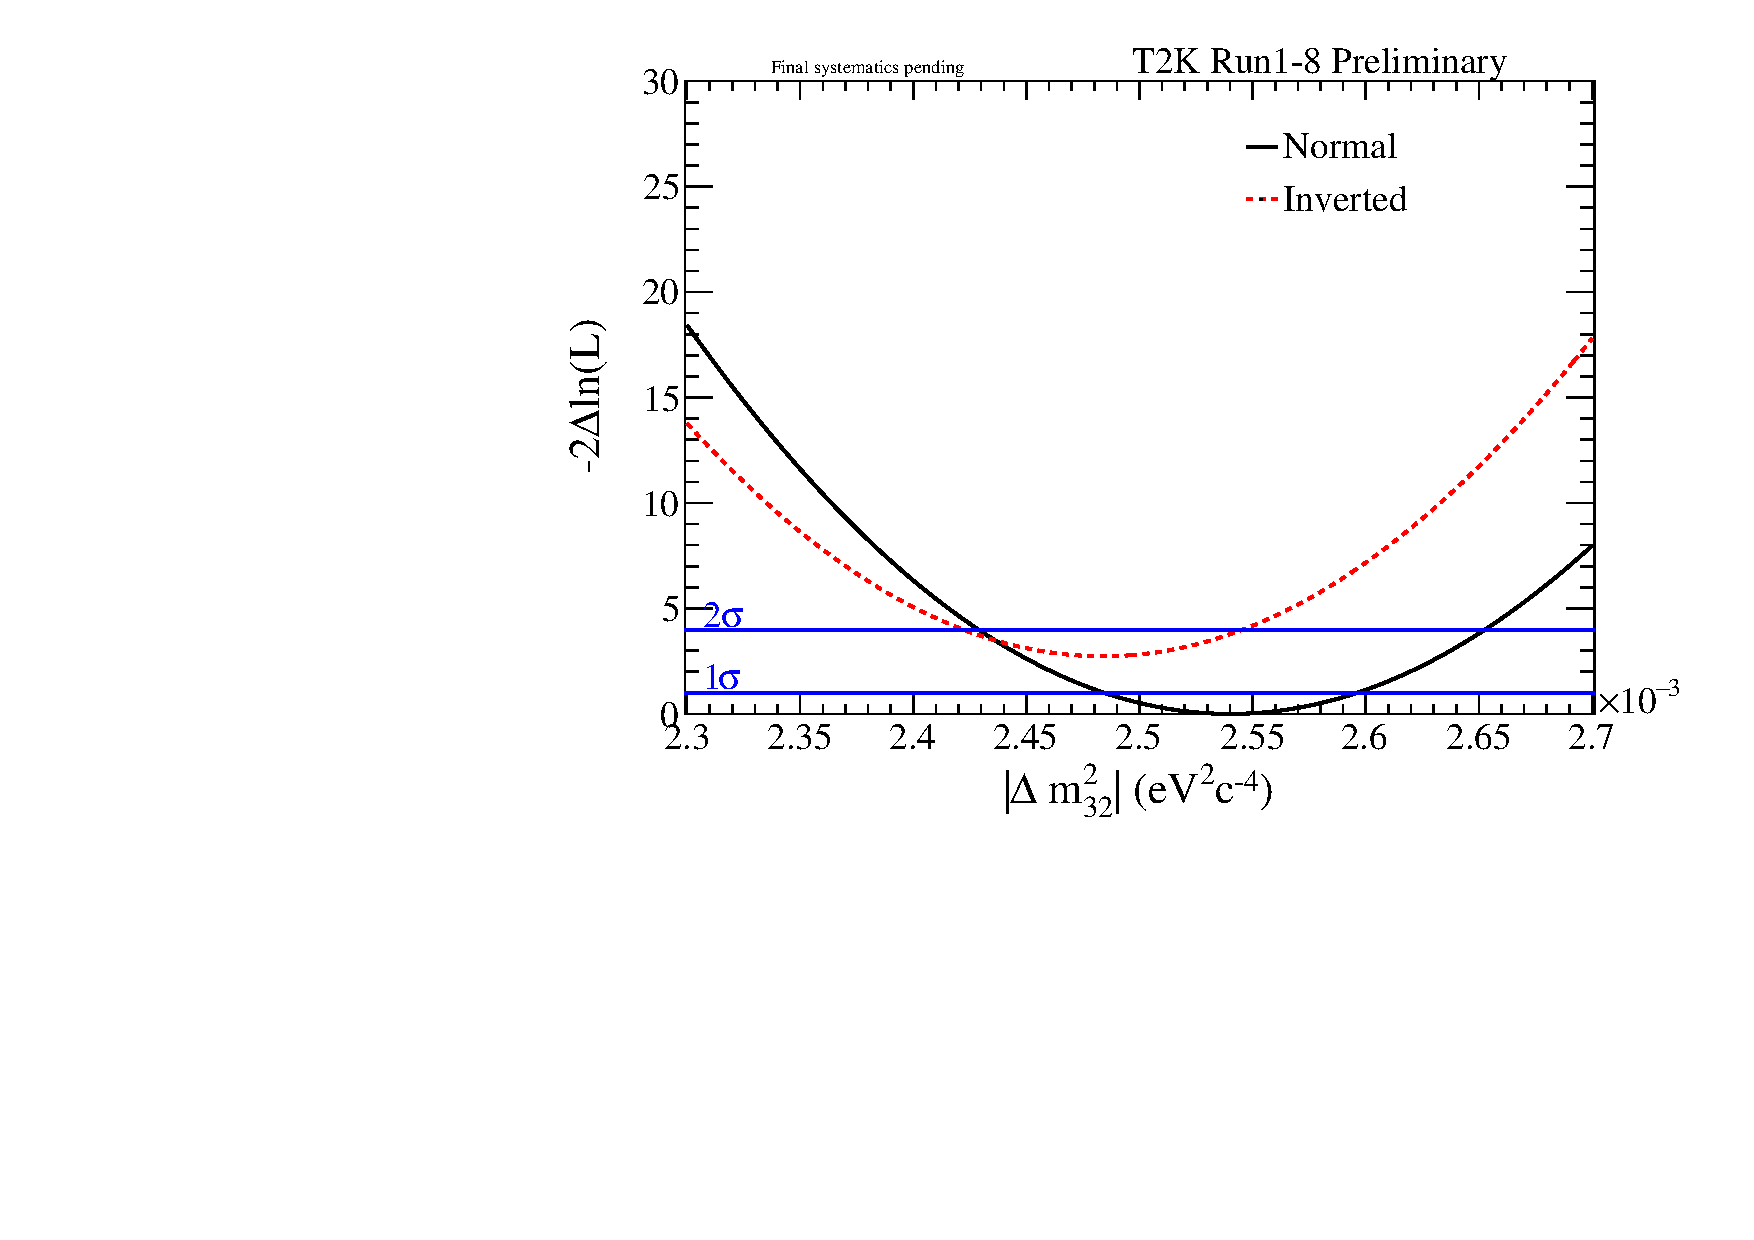
\includegraphics[width=0.9\textwidth]{sensitivity/reactor/dmsq23_AsimovA_reactor_global}
		\caption{Asimov A \dmsqtwothree with reactor constraint}
	\end{subfigure}
	\begin{subfigure}[b]{0.49\textwidth}
		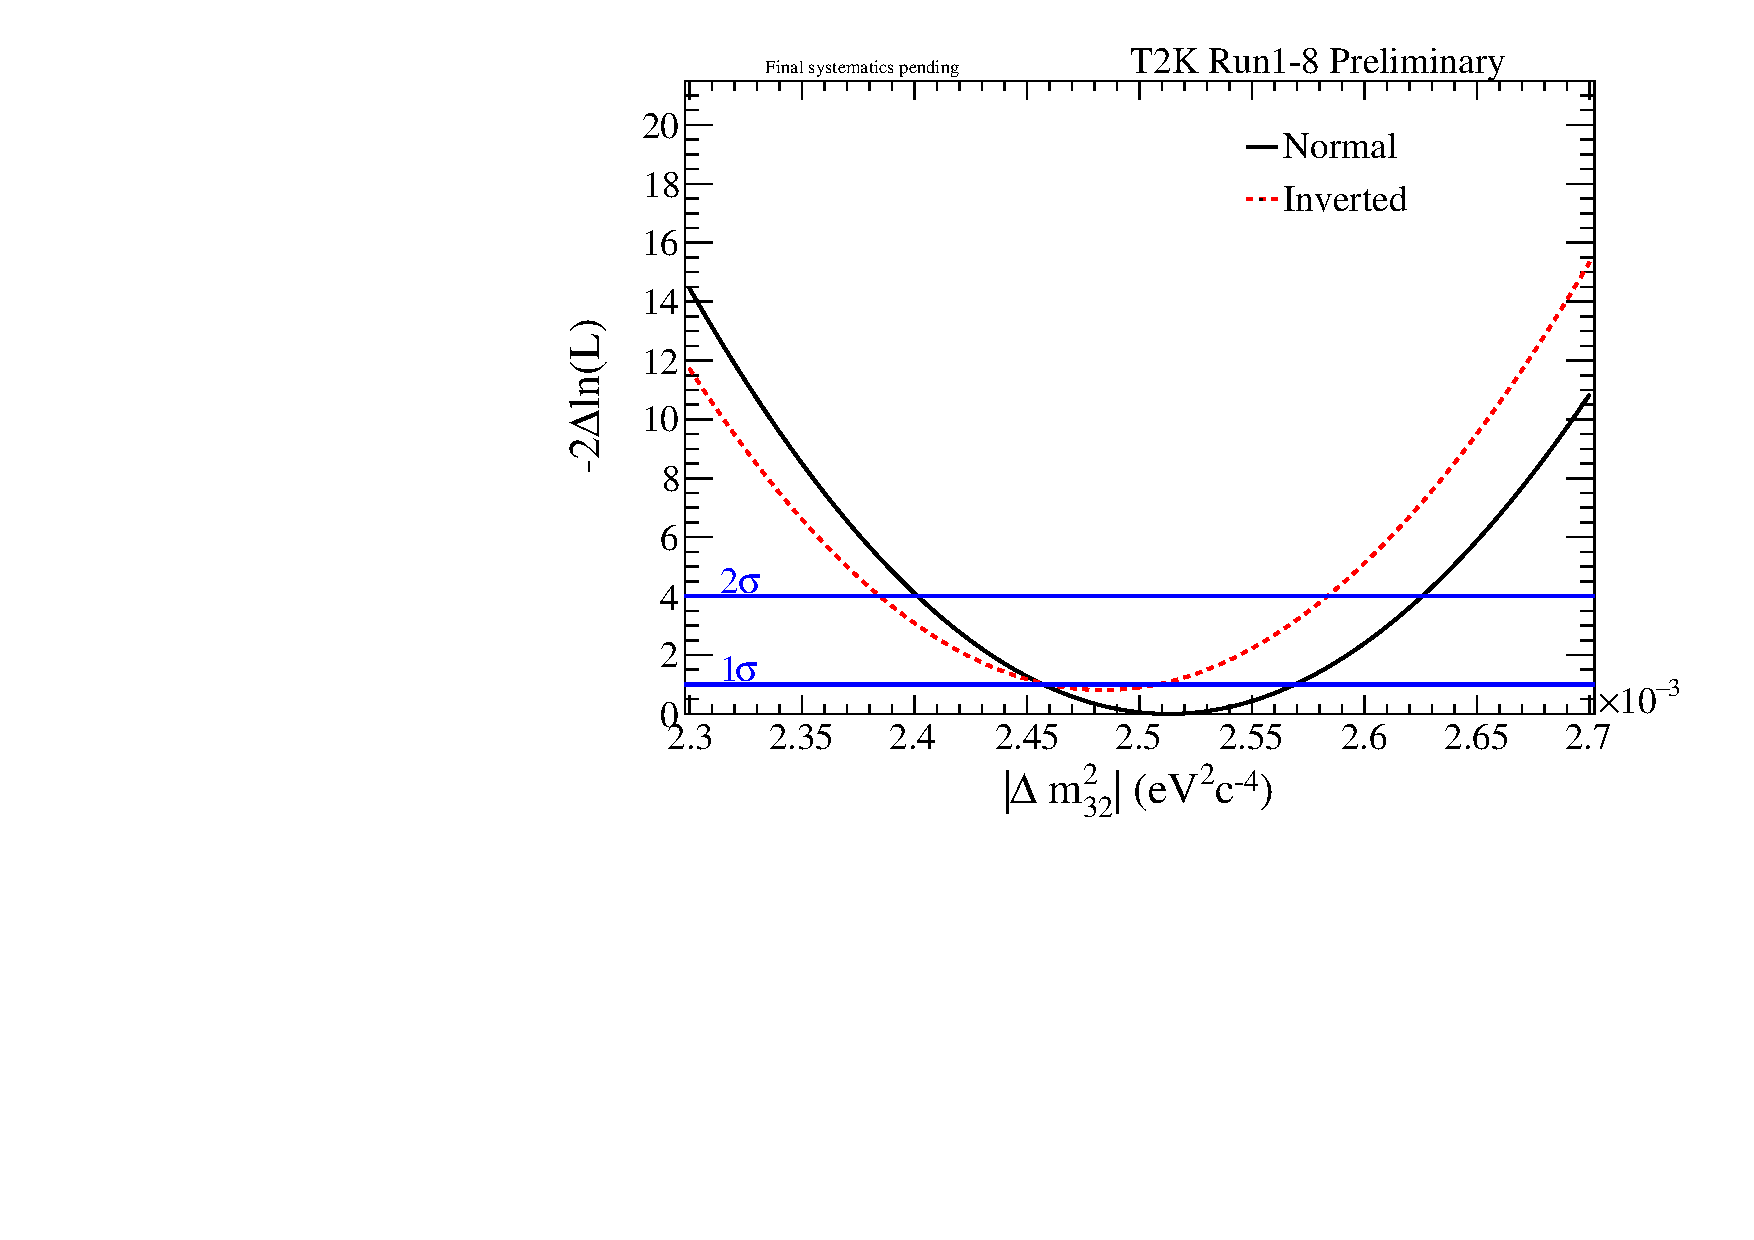
\includegraphics[width=0.9\textwidth]{sensitivity/t2k/dmsq23_AsimovA_t2k_global}
		\caption{Asimov A \dmsqtwothree T2K only}
	\end{subfigure}
	\begin{subfigure}[b]{0.49\textwidth}
		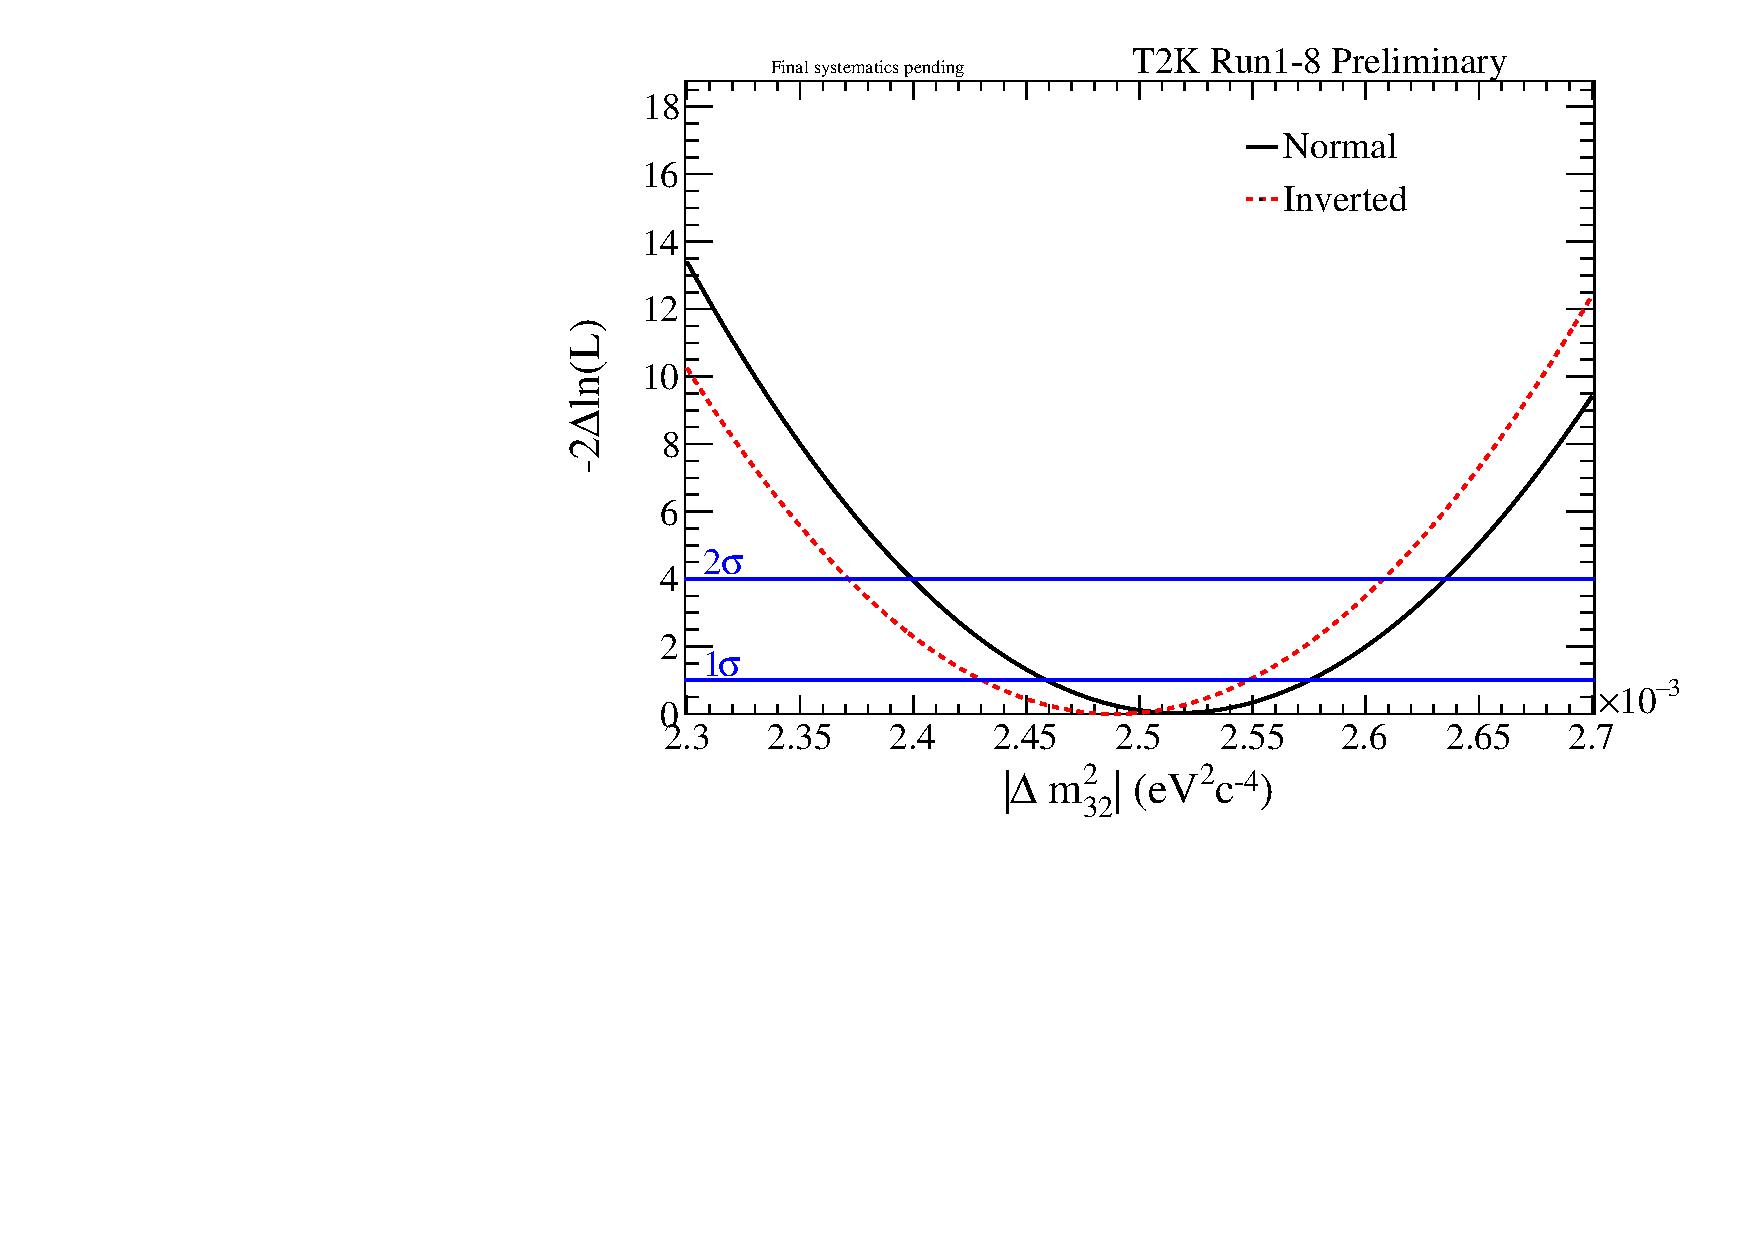
\includegraphics[width=0.9\textwidth]{sensitivity/reactor/dmsq23_AsimovB_reactor_global}
		\caption{Asimov B \dmsqtwothree with reactor constraint}
	\end{subfigure}
	\begin{subfigure}[b]{0.49\textwidth}
		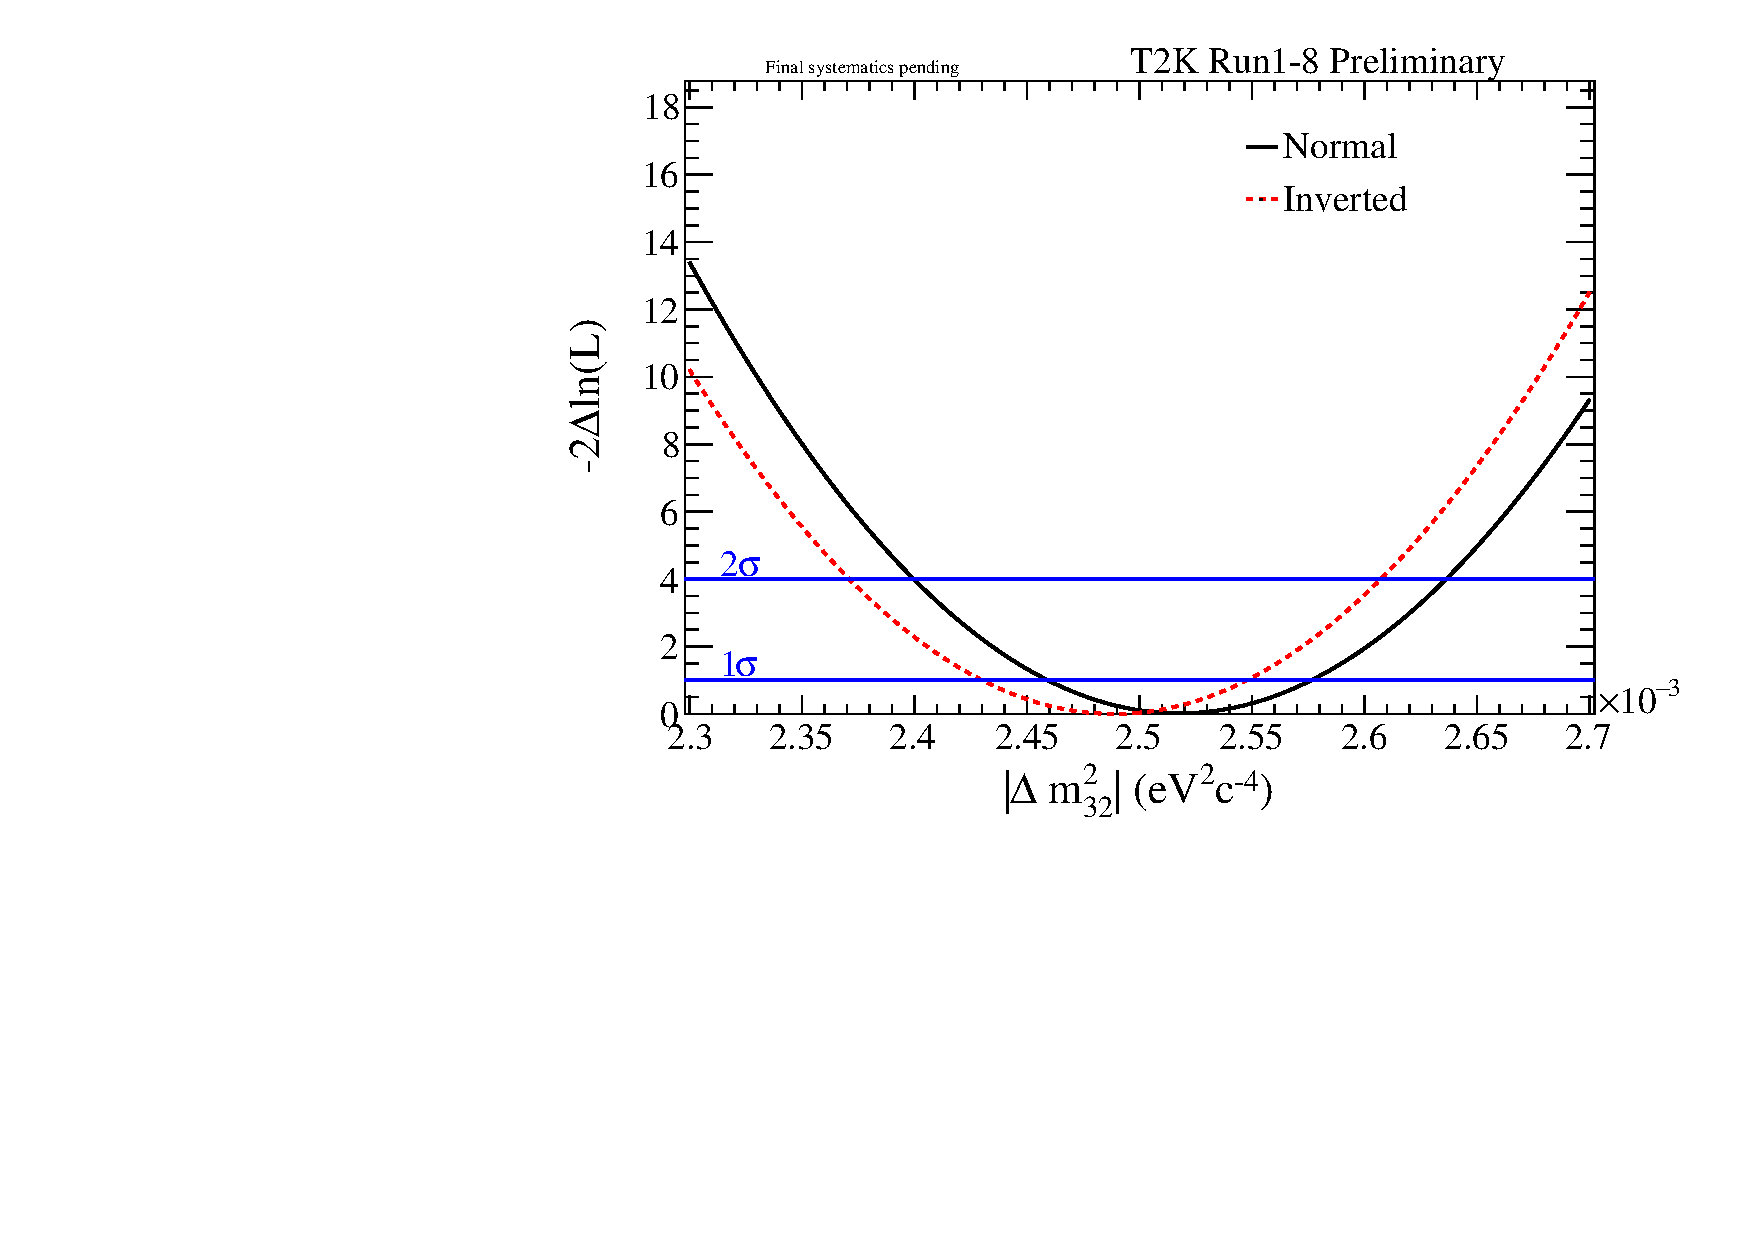
\includegraphics[width=0.9\textwidth]{sensitivity/t2k/dmsq23_AsimovB_t2k_global}
		\caption{Asimov B \dmsqtwothree T2K only}
	\end{subfigure}
	\caption {
		The expected $\Delta\chi^2$ distribution as a function of \dmsqtwothree with and without reactor constraint for Asimov data sets A and B. The mass hierarchy is minimized, with normal and inverted hierarchy $\Delta\chi^2$ distributions shifted to the same global best-fit $\chi^2$ value, which is taken to be the minimum between normal and inverted hierarchy. All 5 samples were used to produce these fits.
	}
	\label{fig:dmsq23_sensitivity}
\end{figure*}

\clearpage

\section {Results of the $\nu\bar{\nu}$ joint analysis with the \RunPeriod dataset}
\label{sec:results}

The results of the \RunPeriod data set fit, for an exposure of \TotalPotNuRunOneEight POT in neutrino mode and of \TotalPotNuBarRunOneEight POT in antineutrino mode, are shown in this chapter. In \cref{fig:asimovpf_spectra_mc_data} the predicted spectra of $\mu$-like and $e$-like samples are compared to the observed data. In \cref{tab:num_events_run18} the expected and observed number of events in \RunPeriod data set are shown. The predicted number of events are shown for the oscillation parameters of Asimov data sets A and B. The comparison of the confidence intervals obtained by the fit of the \RunPeriod data set among all the oscillation analysis groups is shown in \cite{MaCh3:2017}.

\begin{table}[htb]
\centering
\begin{adjustbox}{width=\textwidth, totalheight=\textheight, keepaspectratio}
\begin{tabular}{| c | c | c | c | c | c | c |}
\hline
Beam mode & Sample & Exp. Asimov A & Exp. Asimov A & Exp. Asimov B & Exp. Not Osc & Observed \\
 & & & ($\delta_{CP}=0$) & & & \\
\hline
$\nu$ & $\mu$-like & 268.415 & 268.053 & 280.994 & 1209.918 & 240 \\
$\nu$ & $e$-like & 73.476 & 61.434 & 54.684 & 15.356 & 74 \\
$\bar{\nu}$ & $\mu$-like & 64.278 & 64.123 & 66.010 & 211.548 & 68 \\
$\bar{\nu}$ & $e$-like & 7.911 & 9.023 & 8.187 & 3.243 & 7 \\
$\nu$ & \nueCConepi-like & 6.919 & 6.009 & 5.389 & 2.543 & 15 \\
\hline
\end{tabular}

\end{adjustbox}
\caption{
The observed, expected and best-fit number of events in \RunPeriod data set for an exposure of \TotalPotNuRunOneEight POT in neutrino mode and of \TotalPotNuBarRunOneEight POT in antineutrino mode are shown 
for each selected sample. The prediction is produced using the BANFF tuning and the oscillation parameters shown in \cref{tab:asimov_definition1}.
}
\label{tab:num_events_run18}
\end{table}

The predicted and observed spectra are shown for each of the samples in \cref{fig:asimovpf_spectra_mc_data}. The $e$-like samples are broken down into $E_\text{rec}$ and $\theta$ projections in \cref{fig:asimovpf_spectra_mc_data_elike_1D}.
\begin{figure*}[htb]
	\center
	\begin{subfigure}[b]{0.49\textwidth}
		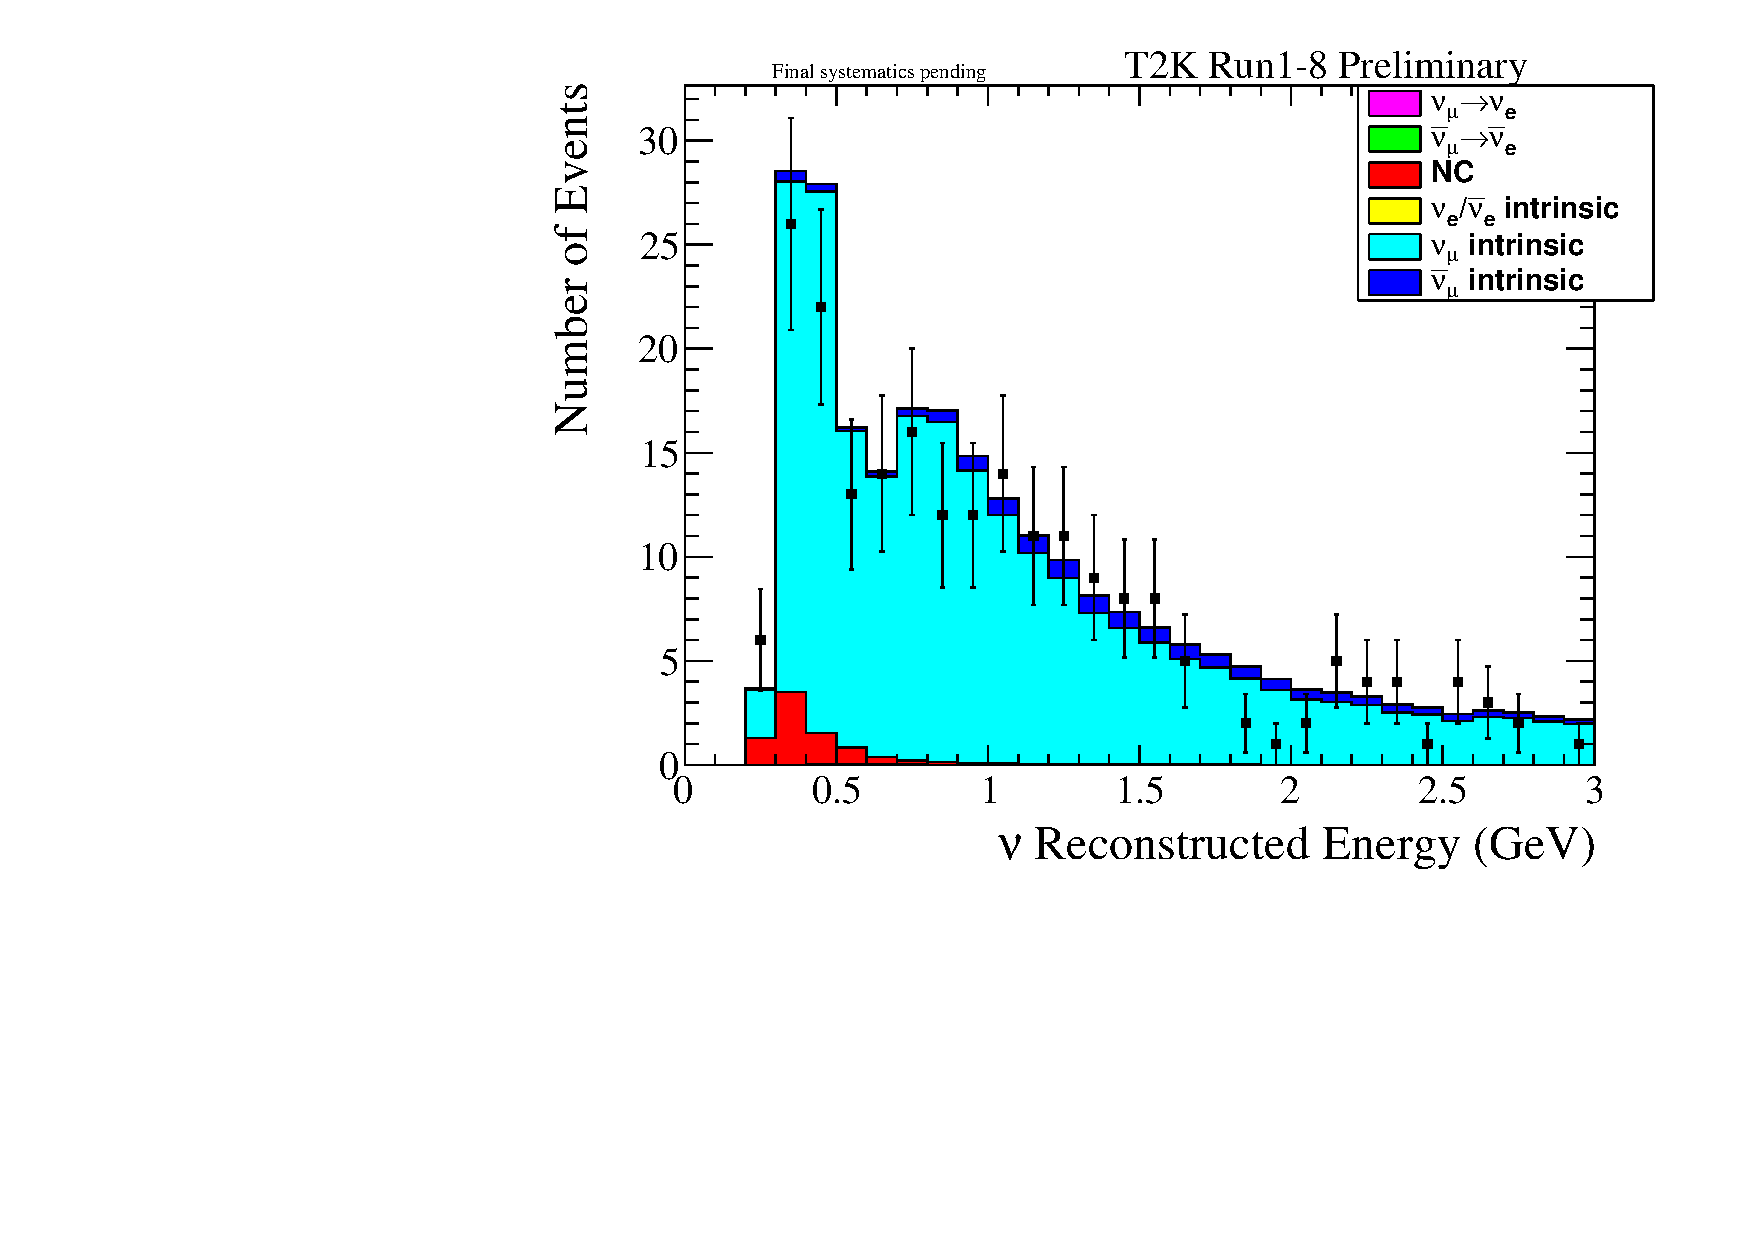
\includegraphics[width=0.9\textwidth]{spectra/spectrum_osc_asimovpf_1Rmu_data}
		\caption{Muon-like, neutrino mode}
	\end{subfigure}
	\begin{subfigure}[b]{0.49\textwidth}
		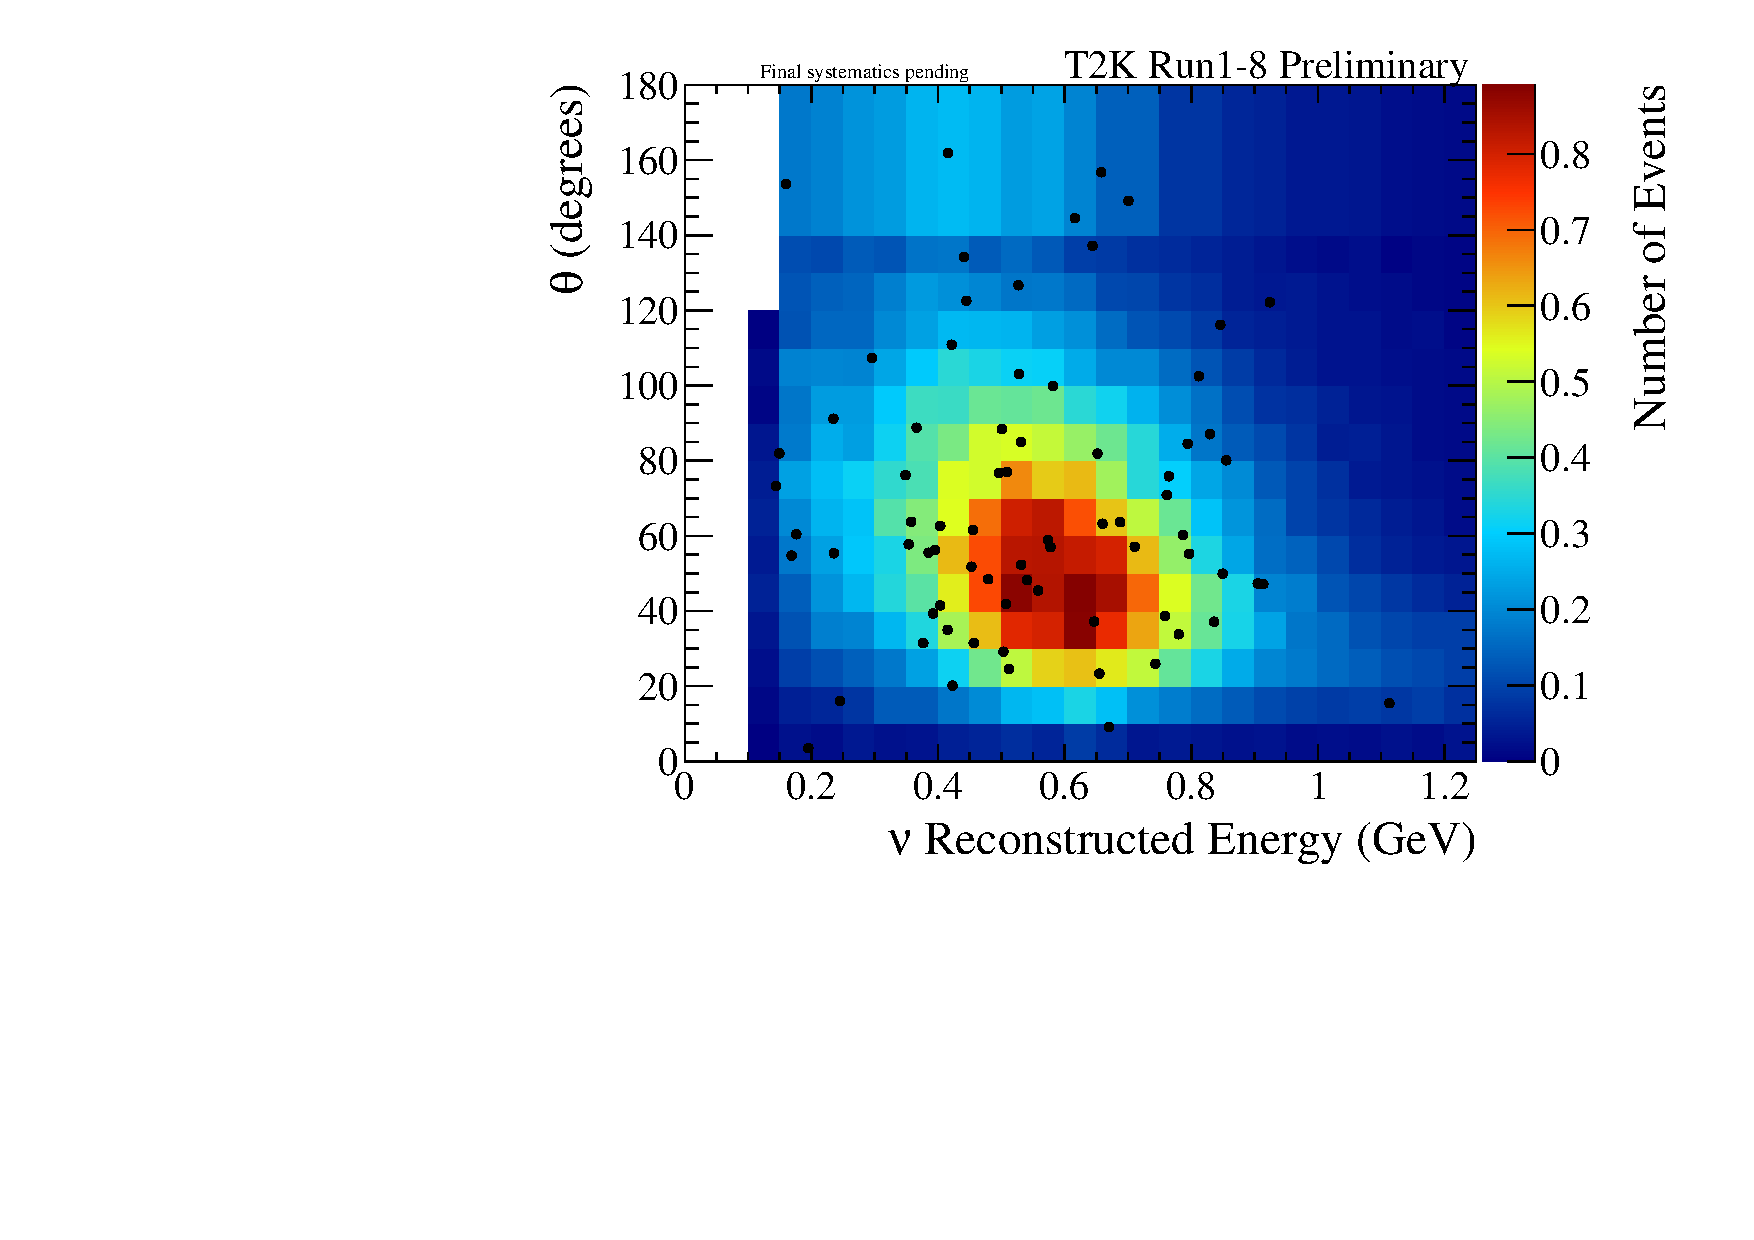
\includegraphics[width=0.9\textwidth]{spectra/spectrum_osc_asimovpf_1Re_data}
		\caption{Electron-like, neutrino mode}
	\end{subfigure}
	\begin{subfigure}[b]{0.49\textwidth}
		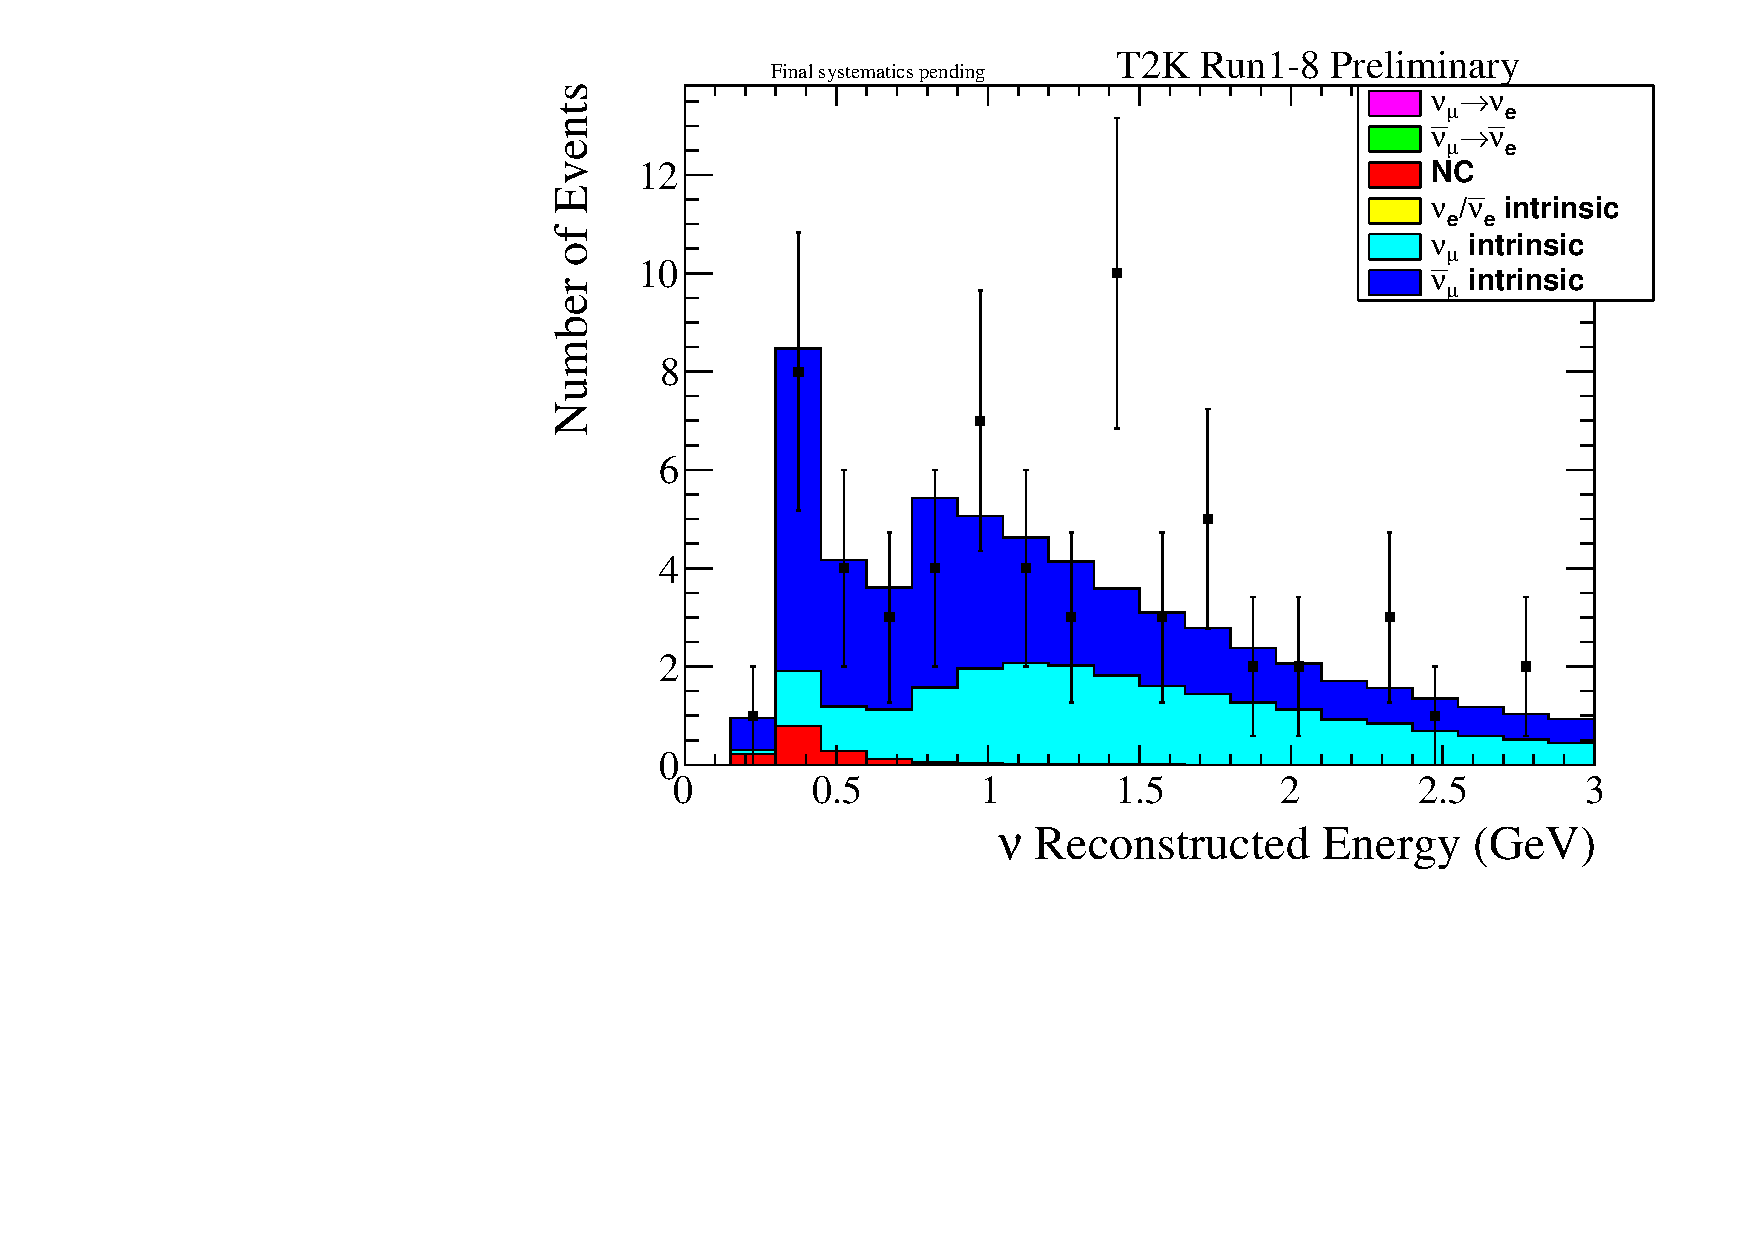
\includegraphics[width=0.9\textwidth]{spectra/spectrum_osc_asimovpf_RHC1Rmu_data}
		\caption{Muon-like, antineutrino mode}
	\end{subfigure}
	\begin{subfigure}[b]{0.49\textwidth}
		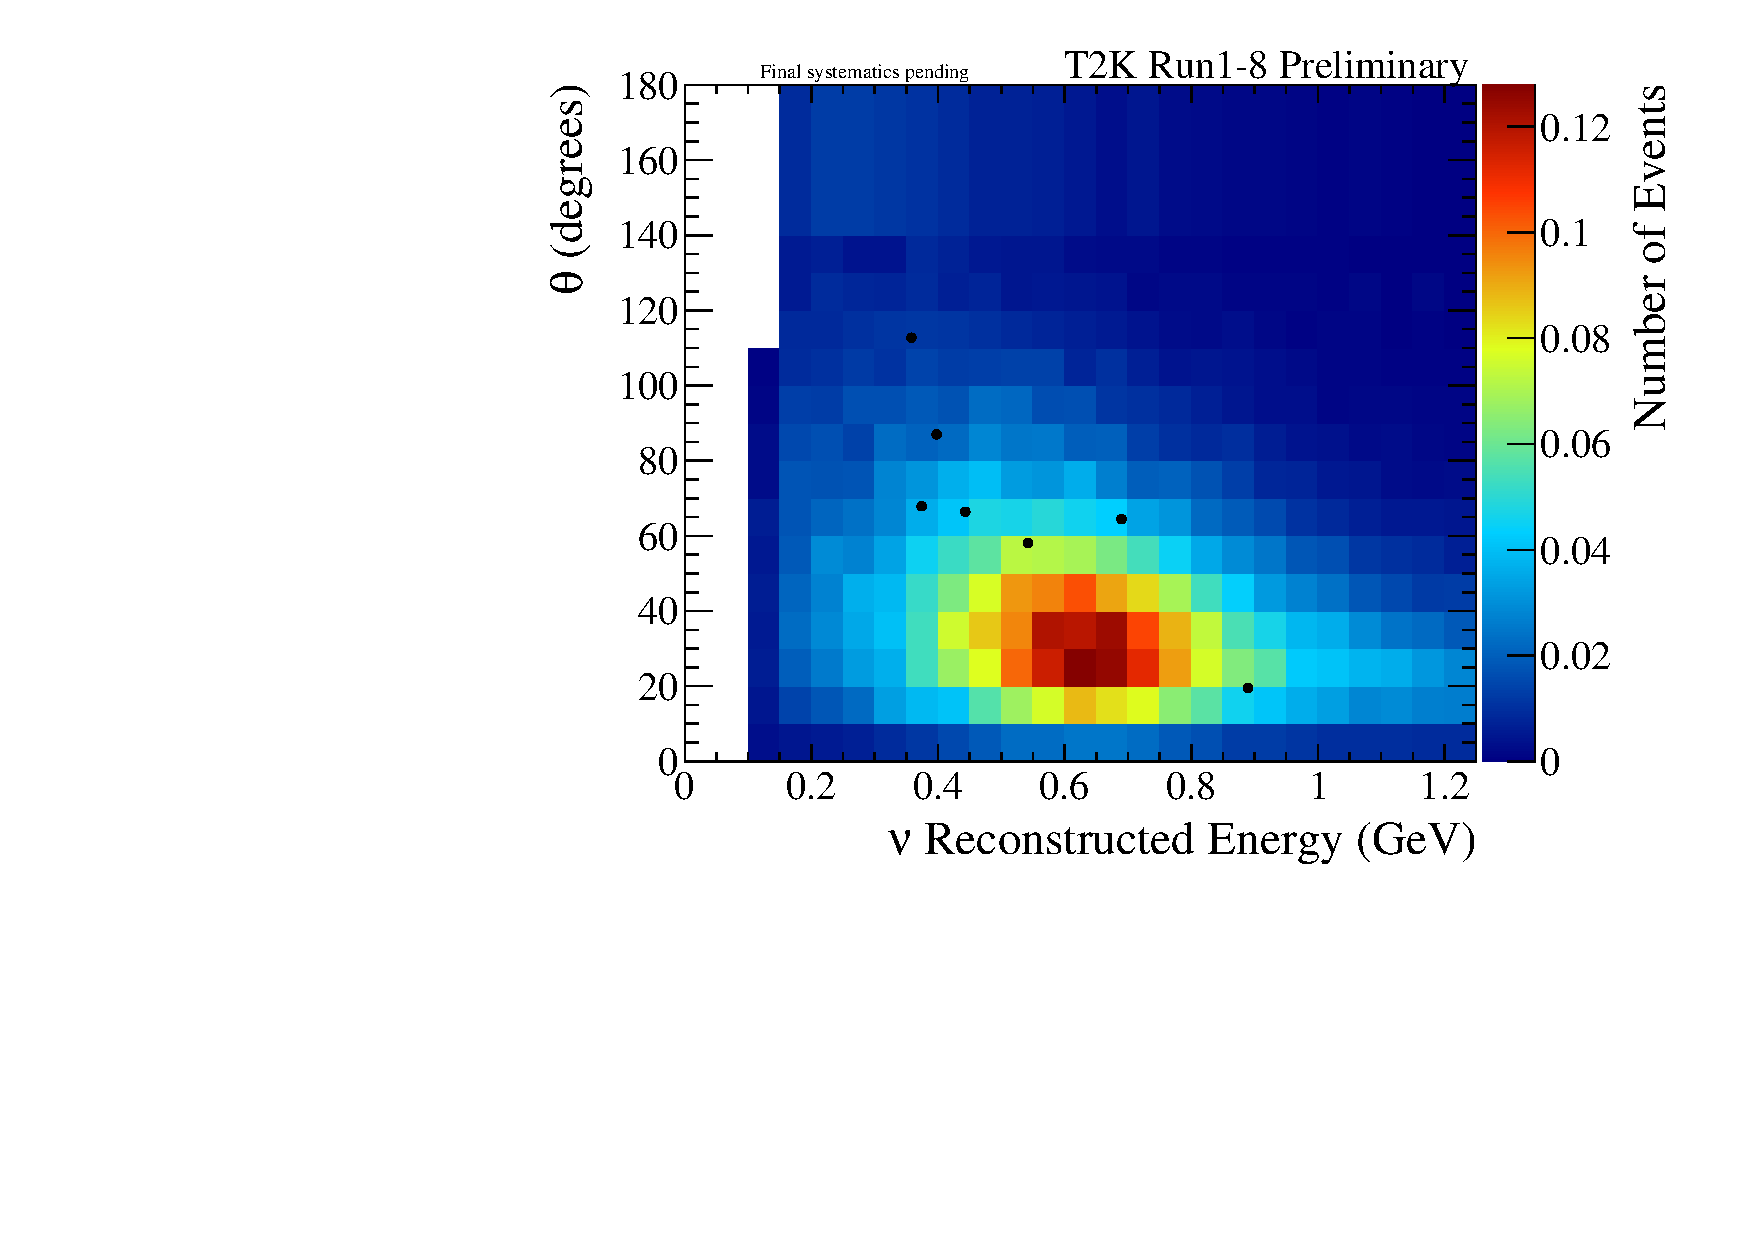
\includegraphics[width=0.9\textwidth]{spectra/spectrum_osc_asimovpf_RHC1Re_data}
		\caption{Electron-like antineutrino mode}
	\end{subfigure}
	\begin{subfigure}[b]{0.49\textwidth}
		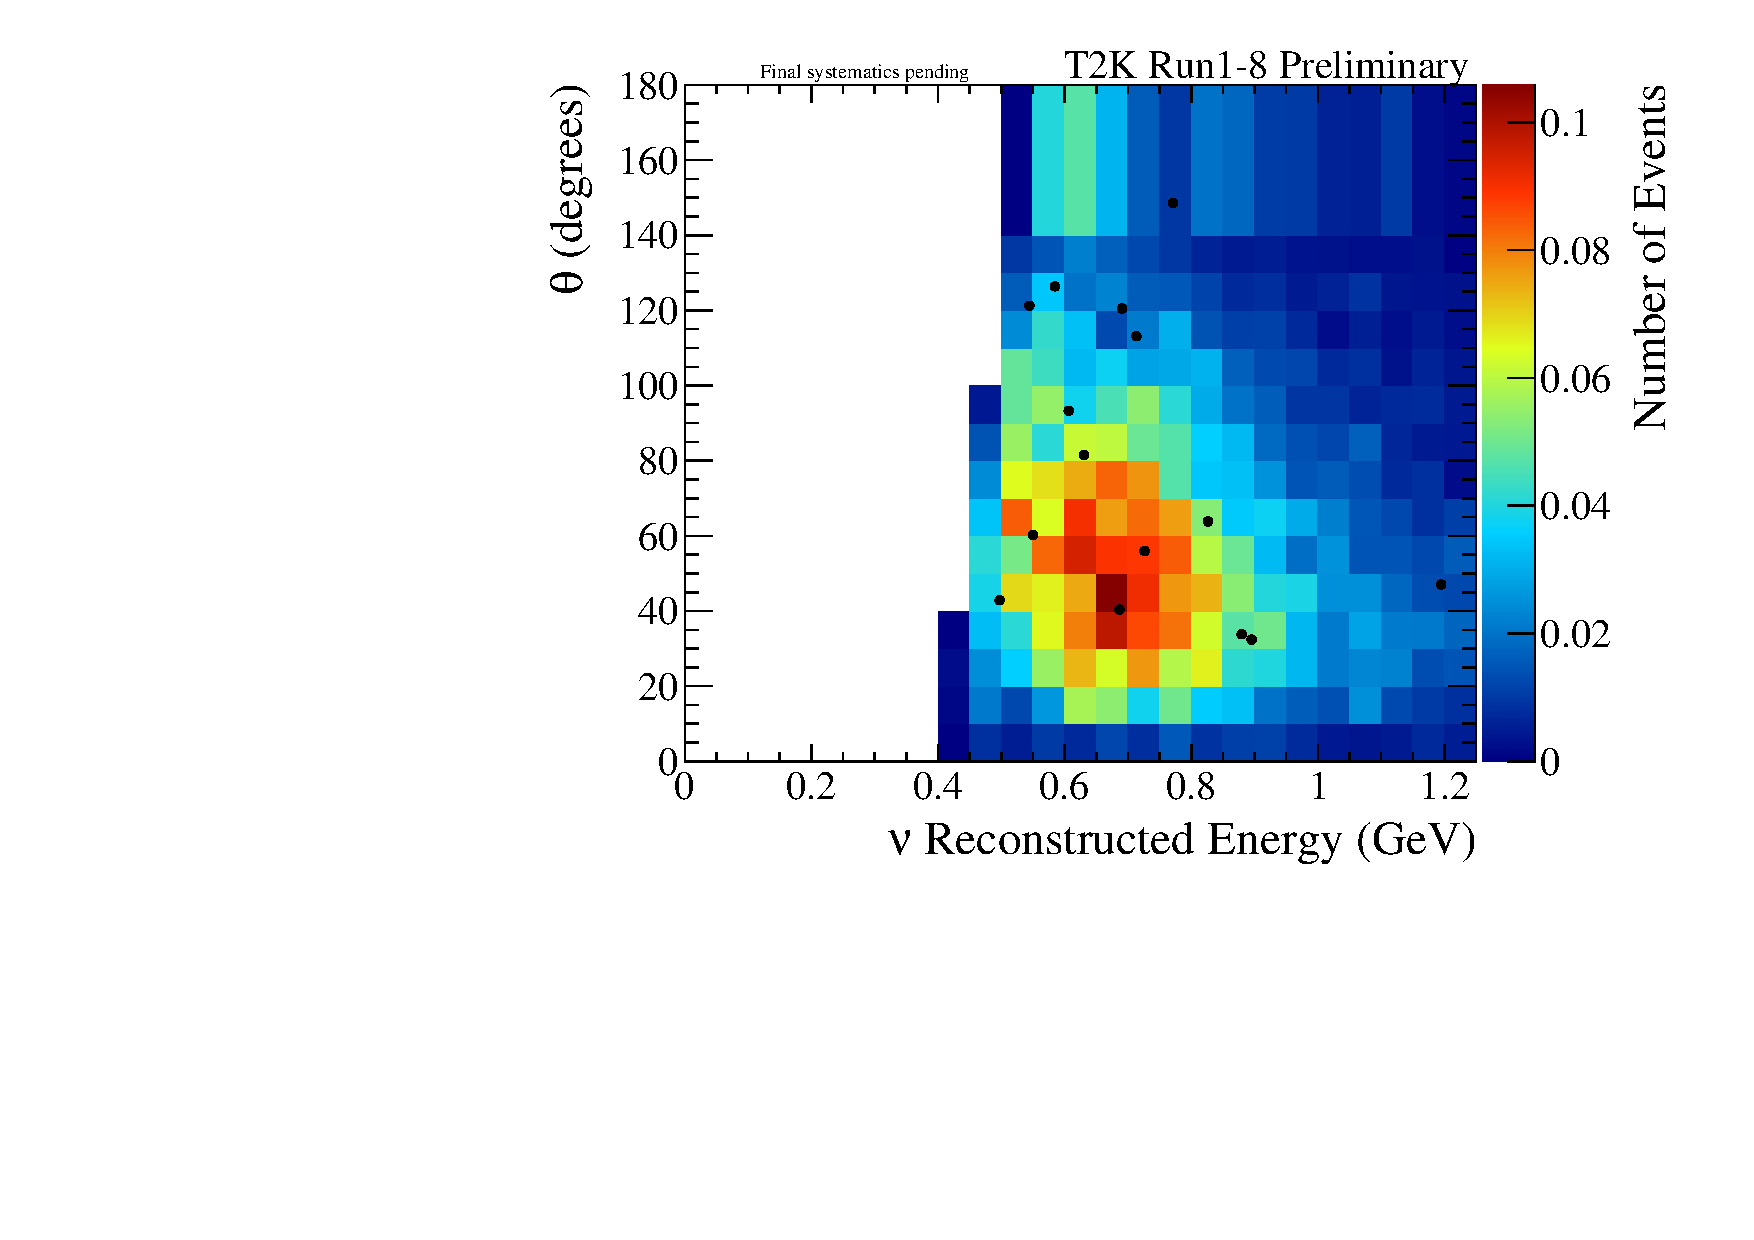
\includegraphics[width=0.9\textwidth]{spectra/spectrum_osc_asimovpf_MultiRe_data}
		\caption{\nueCConepi-like, neutrino mode}
	\end{subfigure}
	\caption {
		Predicted spectra and observed events (points). $\mu$-like distributions are a function of the reconstructed neutrino energy, while the $e$-like, including \nueCConepi, distributions are functions of both the reconstructed neutrino energy and the reconstructed angle between the outgoing lepton and the neutrino direction. The distributions correspond to the statistics collected in the full \RunPeriod data set. The spectra are generated with the systematic parameters described in \cref{sec:systematics} and the oscillation parameters corresponding to the best-fit values from the data fit (solar parameters at PDG 2016).
	}
	\label{fig:asimovpf_spectra_mc_data}
\end{figure*}
\clearpage
\begin{figure*}[htb]
	\center

	\begin{subfigure}[b]{0.49\textwidth}
		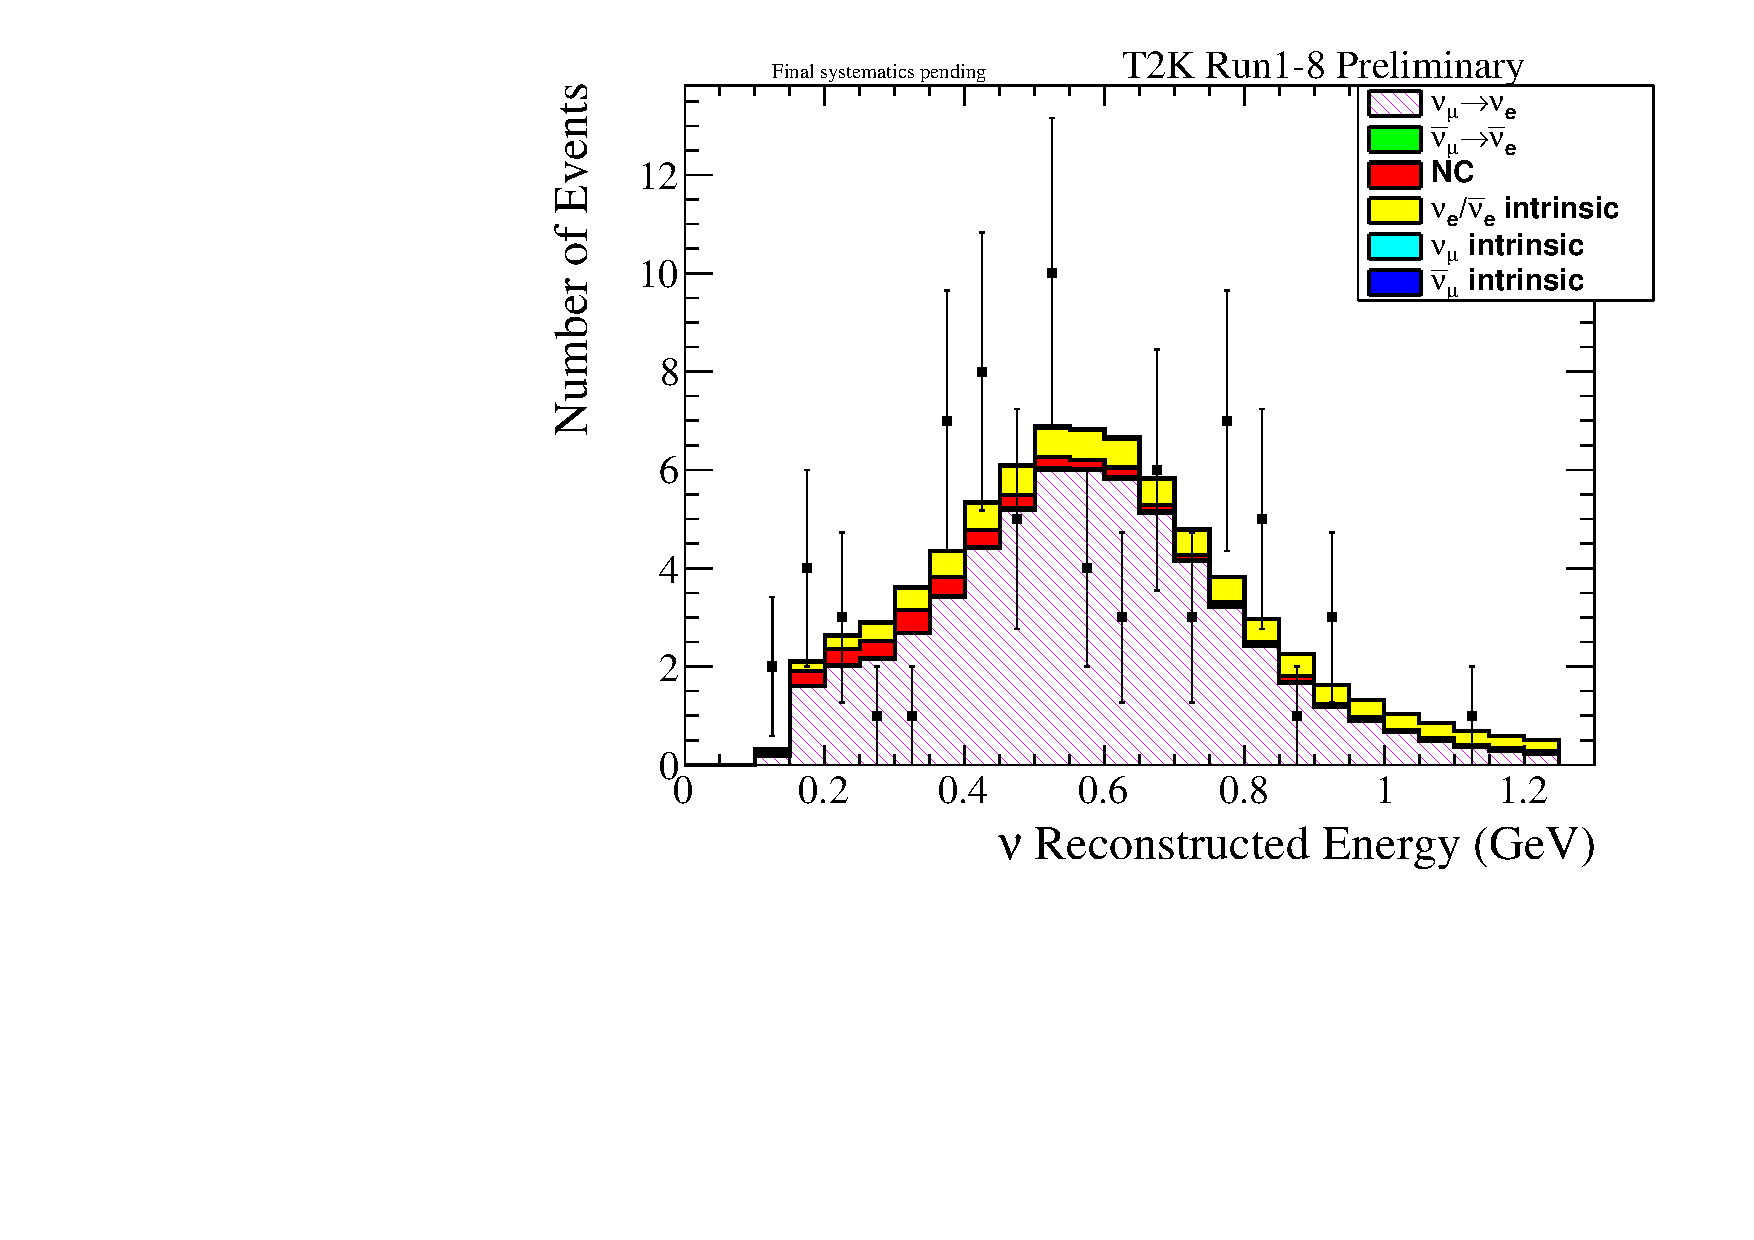
\includegraphics[width=0.9\textwidth]{spectra/erec_spectrum_osc_asimovpf_1Re_data}
		\caption{Electron-like, neutrino mode}
	\end{subfigure}
	\begin{subfigure}[b]{0.49\textwidth}
		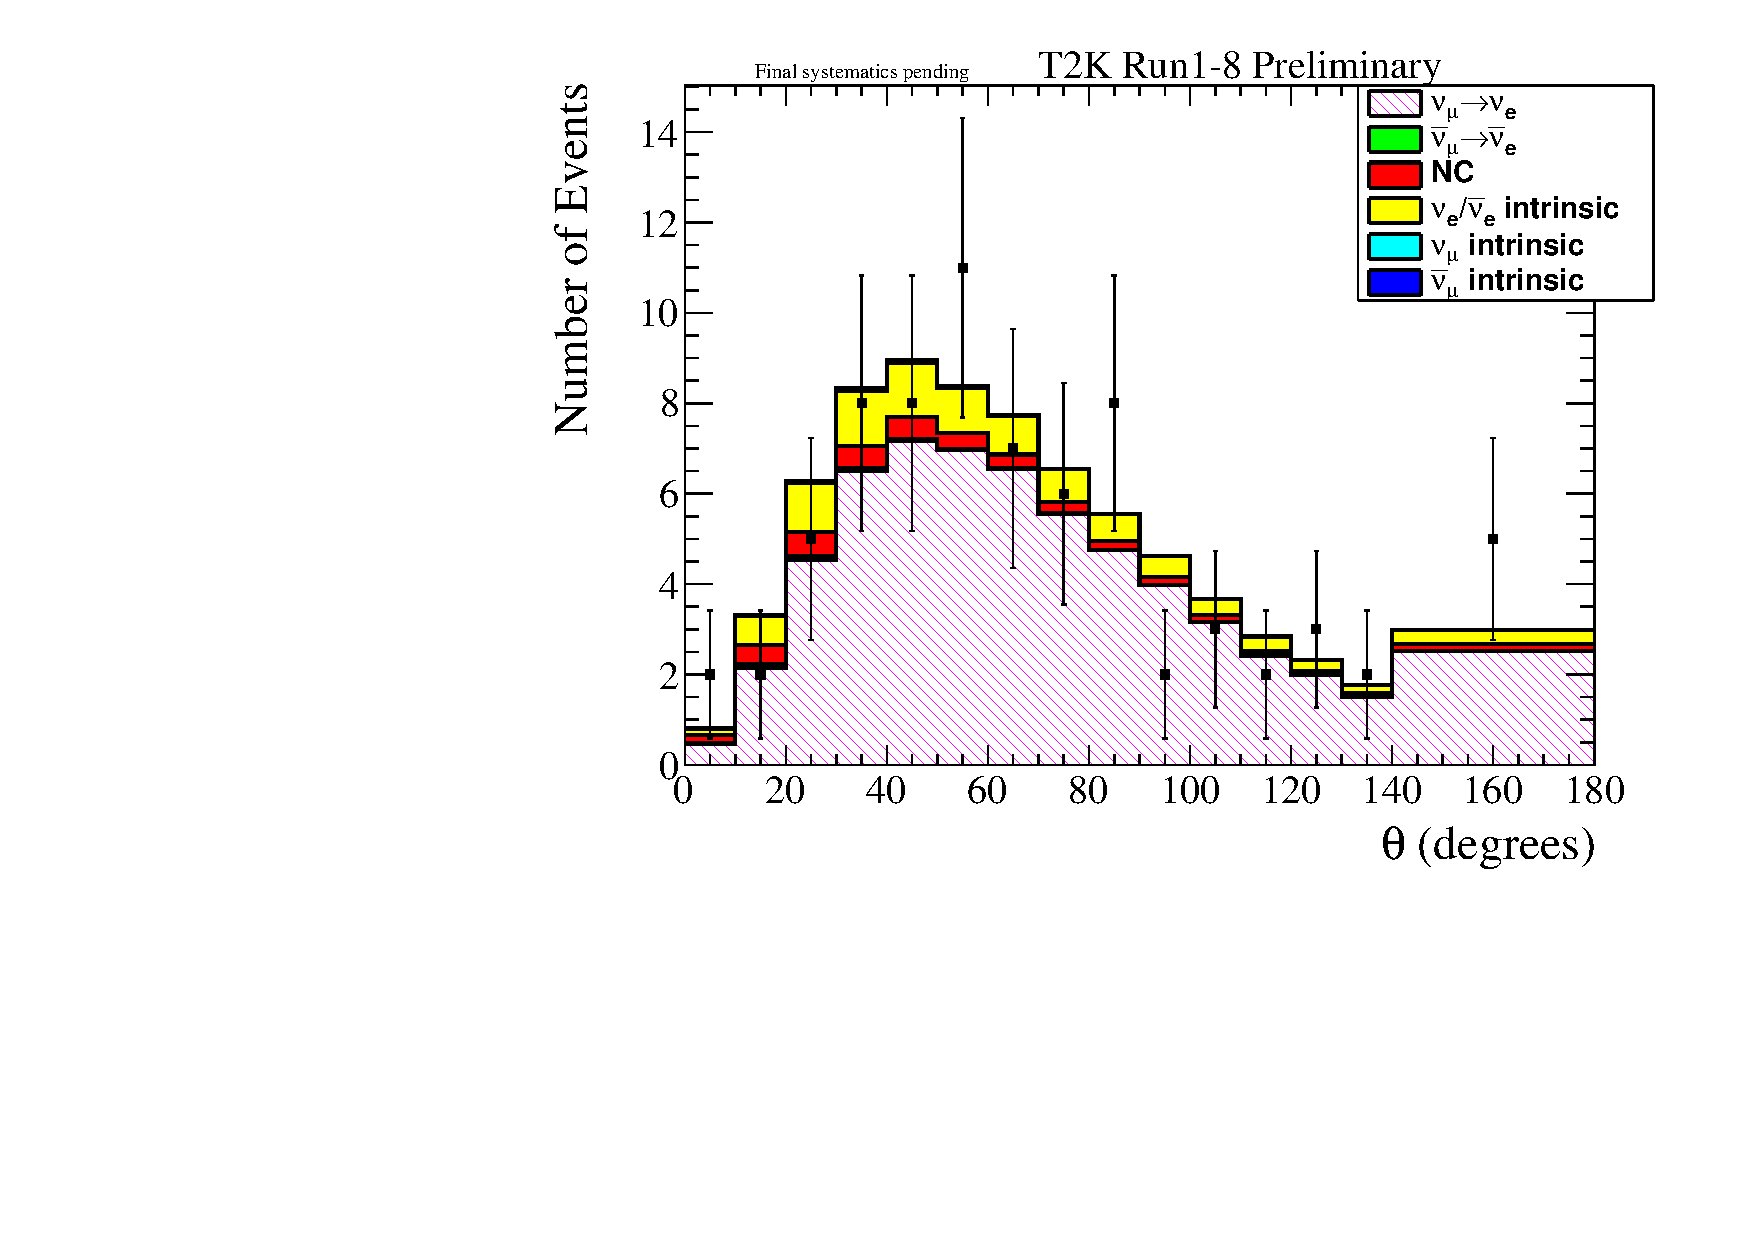
\includegraphics[width=0.9\textwidth]{spectra/theta_spectrum_osc_asimovpf_1Re_data}
		\caption{Electron-like, neutrino mode}
	\end{subfigure}

	\begin{subfigure}[b]{0.49\textwidth}
		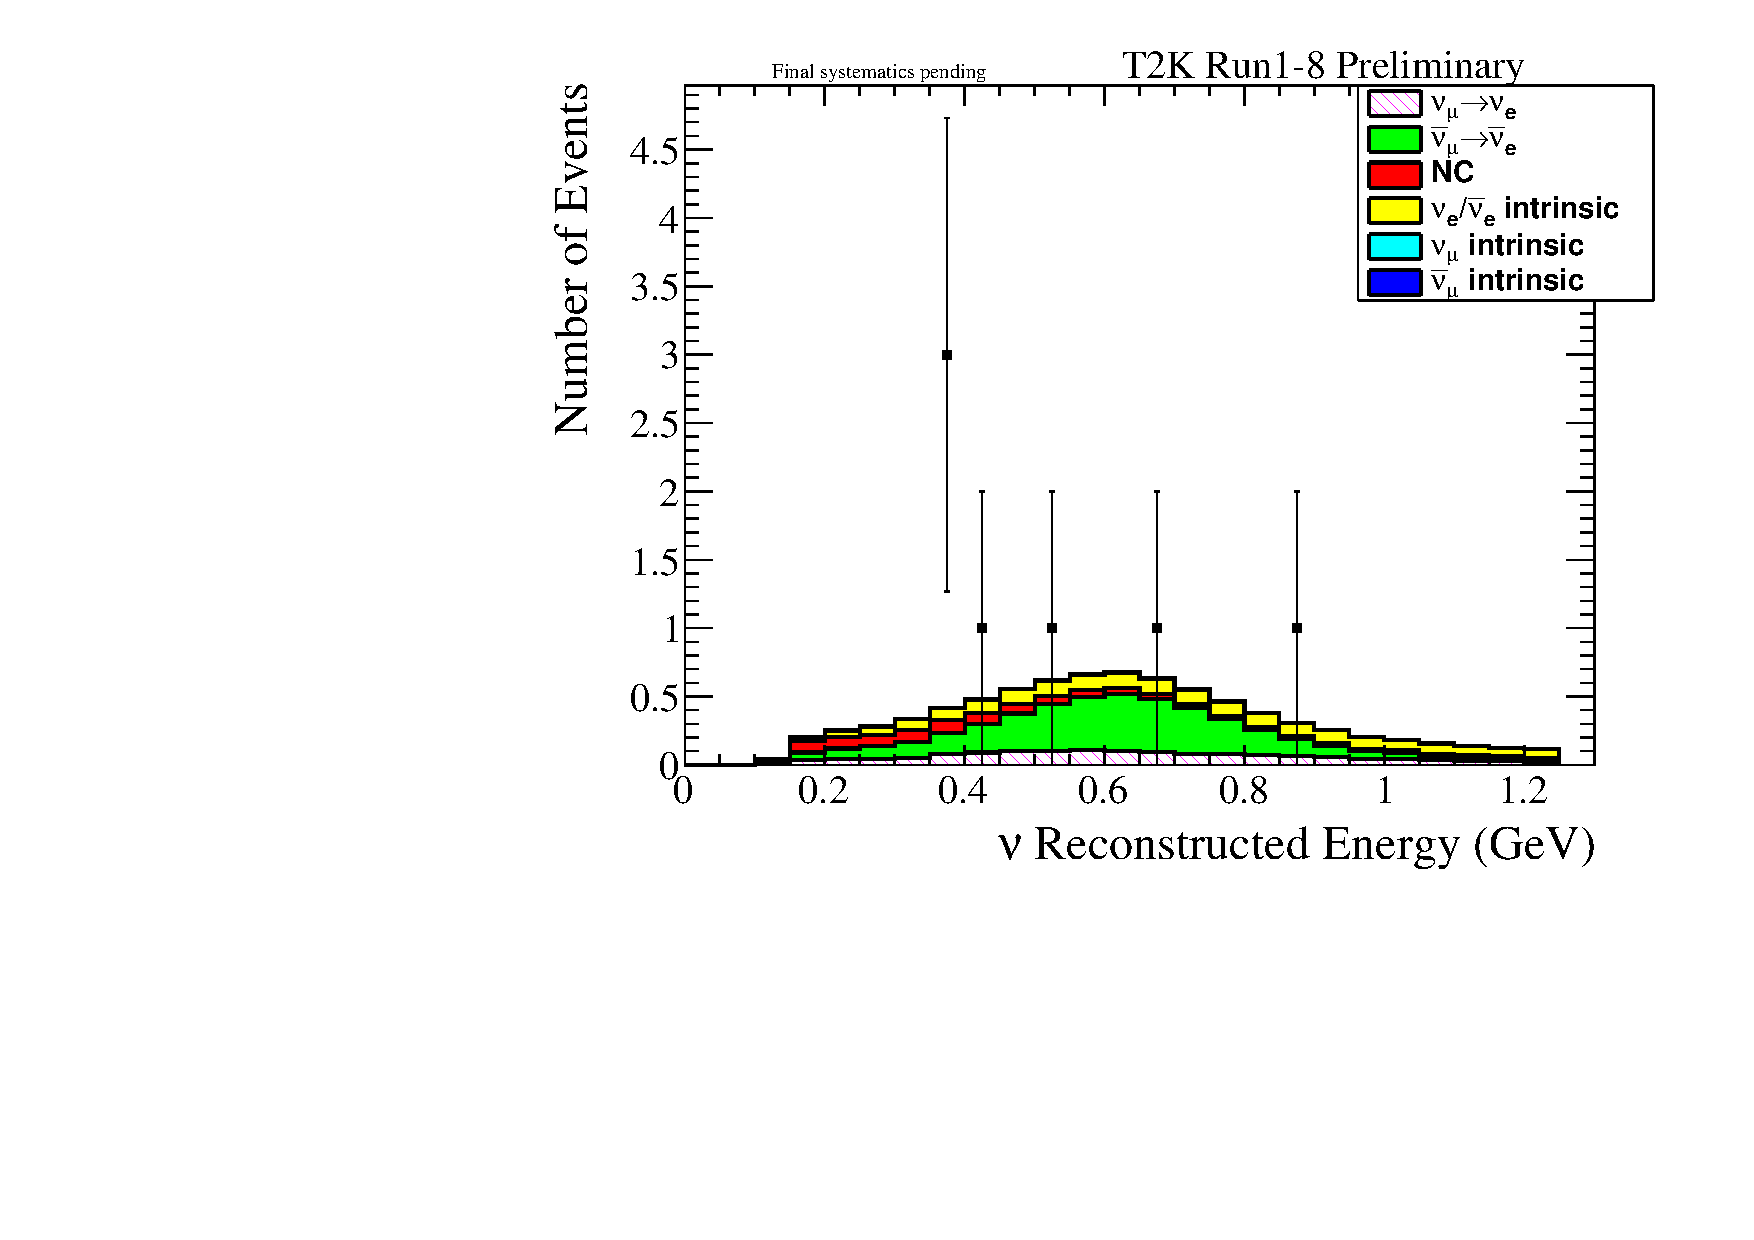
\includegraphics[width=0.9\textwidth]{spectra/erec_spectrum_osc_asimovpf_RHC1Re_data}
		\caption{Electron-like antineutrino mode}
	\end{subfigure}
	\begin{subfigure}[b]{0.49\textwidth}
		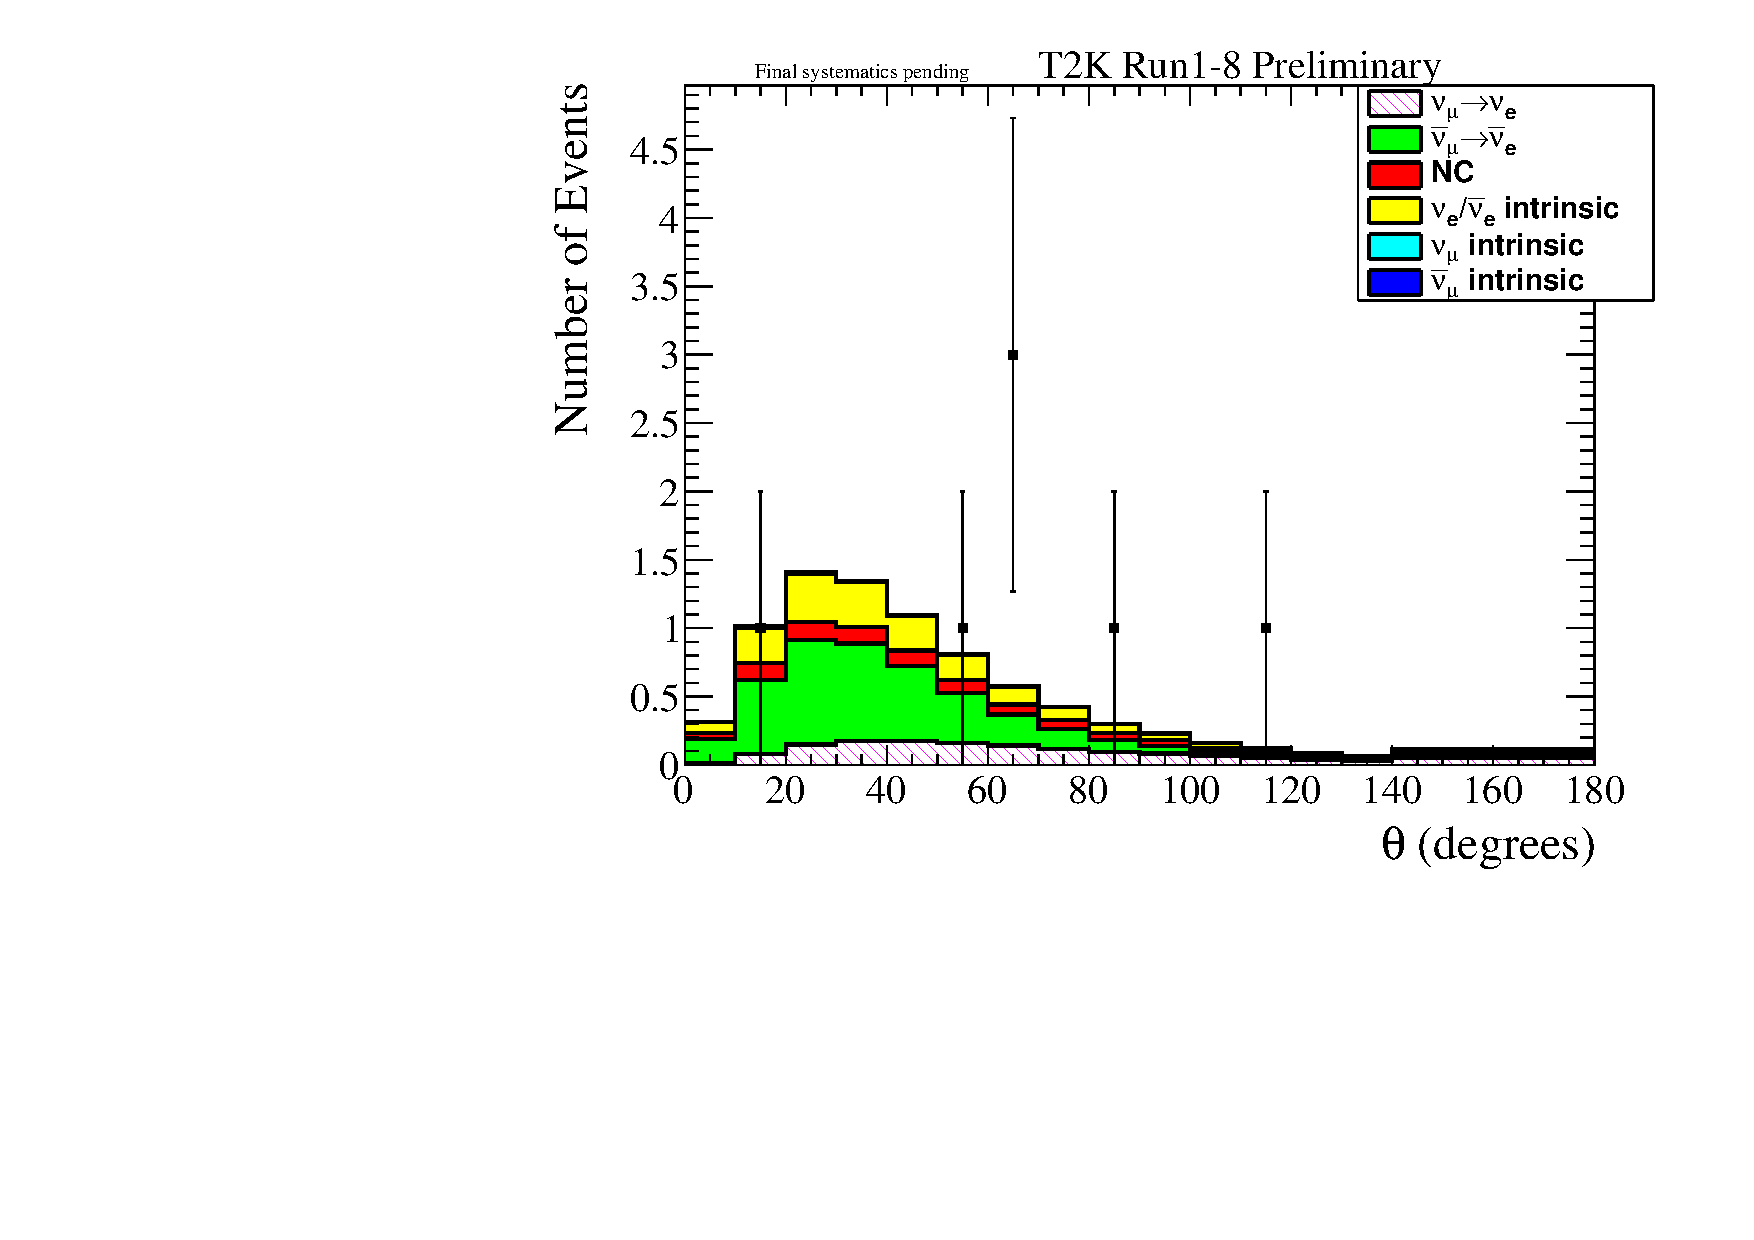
\includegraphics[width=0.9\textwidth]{spectra/theta_spectrum_osc_asimovpf_RHC1Re_data}
		\caption{Electron-like antineutrino mode}
	\end{subfigure}

	\begin{subfigure}[b]{0.49\textwidth}
		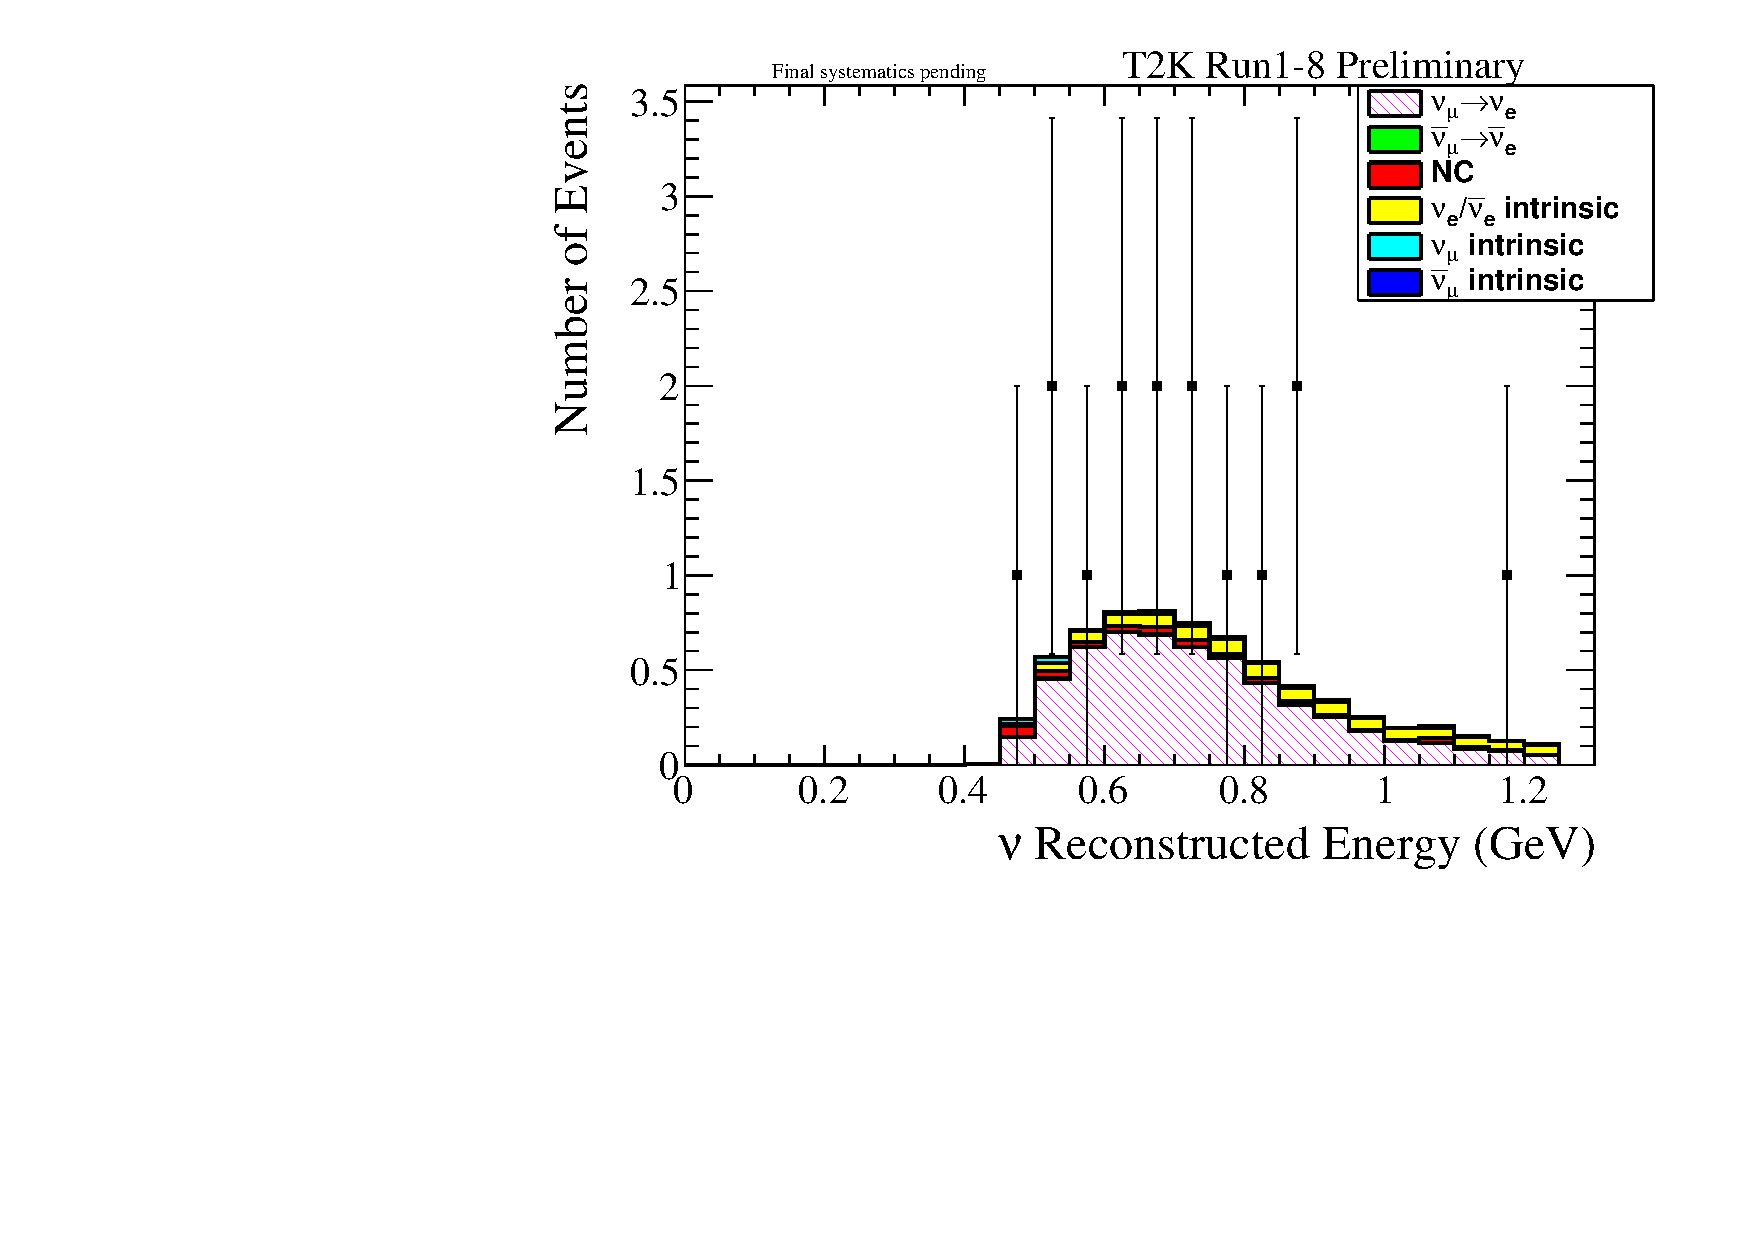
\includegraphics[width=0.9\textwidth]{spectra/erec_spectrum_osc_asimovpf_MultiRe_data}
		\caption{\nueCConepi-like, neutrino mode}
	\end{subfigure}
	\begin{subfigure}[b]{0.49\textwidth}
		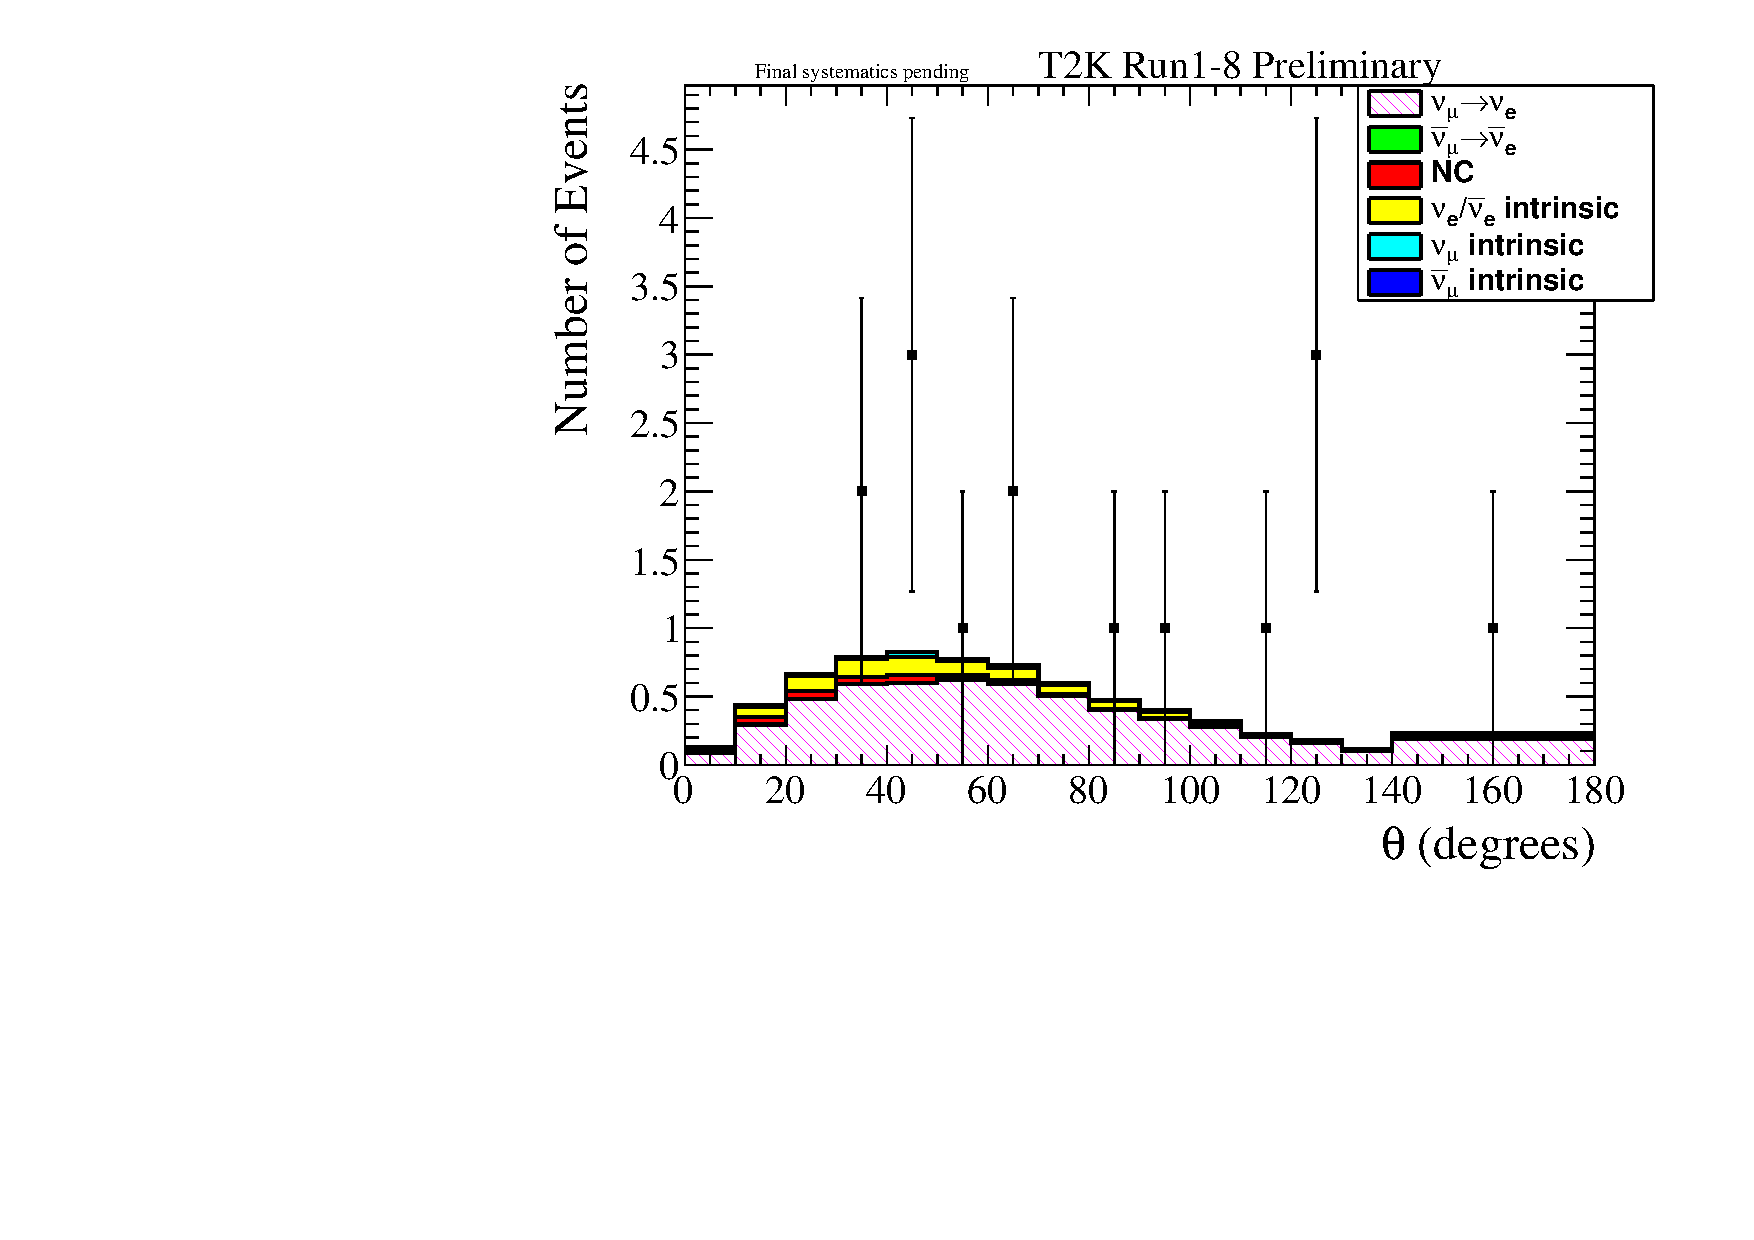
\includegraphics[width=0.9\textwidth]{spectra/theta_spectrum_osc_asimovpf_MultiRe_data}
		\caption{\nueCConepi-like, neutrino mode}
	\end{subfigure}
	\caption {
		Predicted spectra and observed events (points). The $e$-like, including \nueCConepi, distributions are functions of both the reconstructed neutrino energy and the reconstructed angle between the outgoing lepton and the neutrino direction, with the projections in each variable shown here. The distributions correspond to the statistics collected in the full \RunPeriod data set. The spectra are generated with the systematic parameters described in \cref{sec:systematics} and the oscillation parameters corresponding to the best-fit values from the data fit (solar parameters at PDG 2016).
	}
	\label{fig:asimovpf_spectra_mc_data_elike_1D}
\end{figure*}
\clearpage

The best-fit values and $1\sigma$ ranges for each oscillation parameter are shown in \cref{tab:data_bestfit} for normal hierarchy (which is preferred in all data fits). The $1\sigma$ ranges are extracted for each oscillation parameter from the 1-dimensional $\Delta \chi^2$ distributions shown in \crefrange{fig:dcp_data}{fig:dmsq23_data}.

The 1-dimensional contours are plotted with respect to the global minimum from normal and inverted hierarchies, while the 2-dimensional confidence intervals are shown drawing the normal and inverted hierarchy contours independently, i.e. each contour is produced with respect to the global minimum under that hierarchy hypothesis.

%The reactor measurements are in agreement with the T2K data at $1\sigma$ level if $\delta_{CP} \sim - \frac{\pi}{2}$. Furthermore we can see that the region close $\delta_{CP} = + \pi/2$ is excluded at 90\% CL.

\begin{table}
\centering
\begin{tabular}{| c | c | c | c | c | c |}
\hline
Parameter & Reactor & Best-fit (NH) & $\pm1\sigma$ (NH) & Best-fit (IH) & $\pm1\sigma$ (IH) \\
\hline
\deltacp & Yes & \BestFitDeltacpwRC & [\MOneSigmaDeltacpwRC,\POneSigmaDeltacpwRC] & \BestFitDeltacpwRCIH & [\MOneSigmaDeltacpwRCIH,\POneSigmaDeltacpwRCIH] \\
\deltacp & No & \BestFitDeltacpwoRC & [\MOneSigmaDeltacpwoRC,\POneSigmaDeltacpwoRC] & \BestFitDeltacpwoRCIH & [\MOneSigmaDeltacpwoRCIH,\POneSigmaDeltacpwoRCIH] \\
\ssqthonethree & No & \BestFitMixingOneThreewoRC & [\MOneMixingOneThreewoRC,\POneMixingOneThreewoRC] & \BestFitMixingOneThreewoRCIH & [\MOneMixingOneThreewoRCIH,\POneMixingOneThreewoRCIH] \\
\ssqthtwothree & Yes & \BestFitMixingTwoThreewRC & [\MOneMixingTwoThreewRC,\POneMixingTwoThreewRC] & \BestFitMixingTwoThreewRCIH & [\MOneMixingTwoThreewRCIH,\POneMixingTwoThreewRCIH] \\
\dmsqtwothree or \dmsqonethree & Yes & \BestFitDmTwoThreewRC & [\MOneDmTwoThreewRC,\POneDmTwoThreewRC] & \BestFitDmTwoThreewRCIH & [\MOneDmTwoThreewRCIH,\POneDmTwoThreewRCIH] \\
 ($10^{-3}\text{ eV}^2\text{/c}^4$) & & & & & \\
\hline
\end{tabular}

\caption{
The \RunPeriod measured oscillation parameter best-fit and the $\pm 1\sigma$ intervals are shown for normal and inverted hierarchies with respect to the hierarchy best-fit. The $\pm 1\sigma$ interval is obtained by using the constant $\Delta \chi^2$ method. For each parameter normal hierarchy is the global best-fit.
}
\label{tab:data_bestfit}
\end{table}

\clearpage

\subsection{Results for \appearance}
In \cref{fig:ssqth13_vs_dcp_data} the result for \appearance with reactor constraint and T2K only is shown.

\begin{figure*}[htb]
	\center
	\begin{subfigure}[b]{0.49\textwidth}
		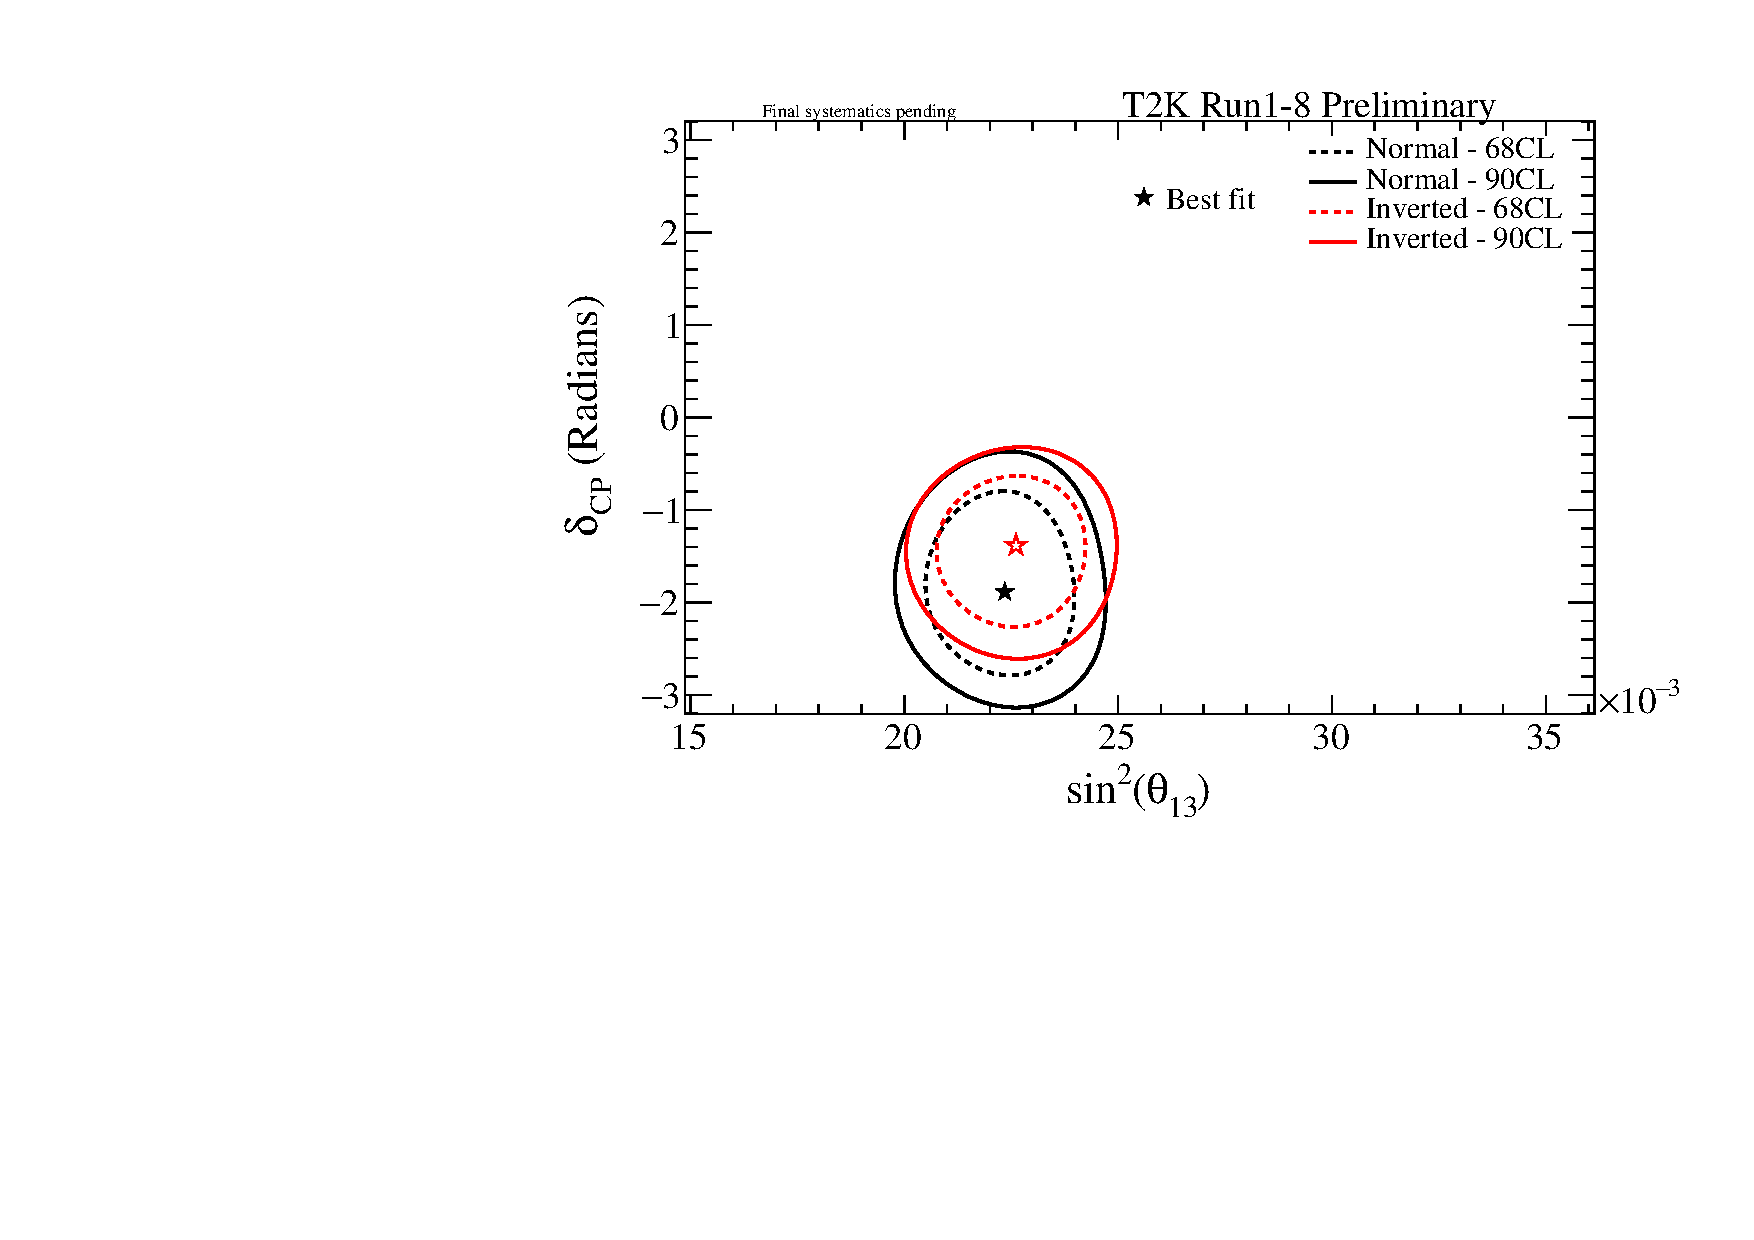
\includegraphics[width=0.9\textwidth]{data/reactor/mixing13_deltacp_data_reactor_global}
		\caption{\appearance with reactor constraint}
	\end{subfigure}
	\begin{subfigure}[b]{0.49\textwidth}
		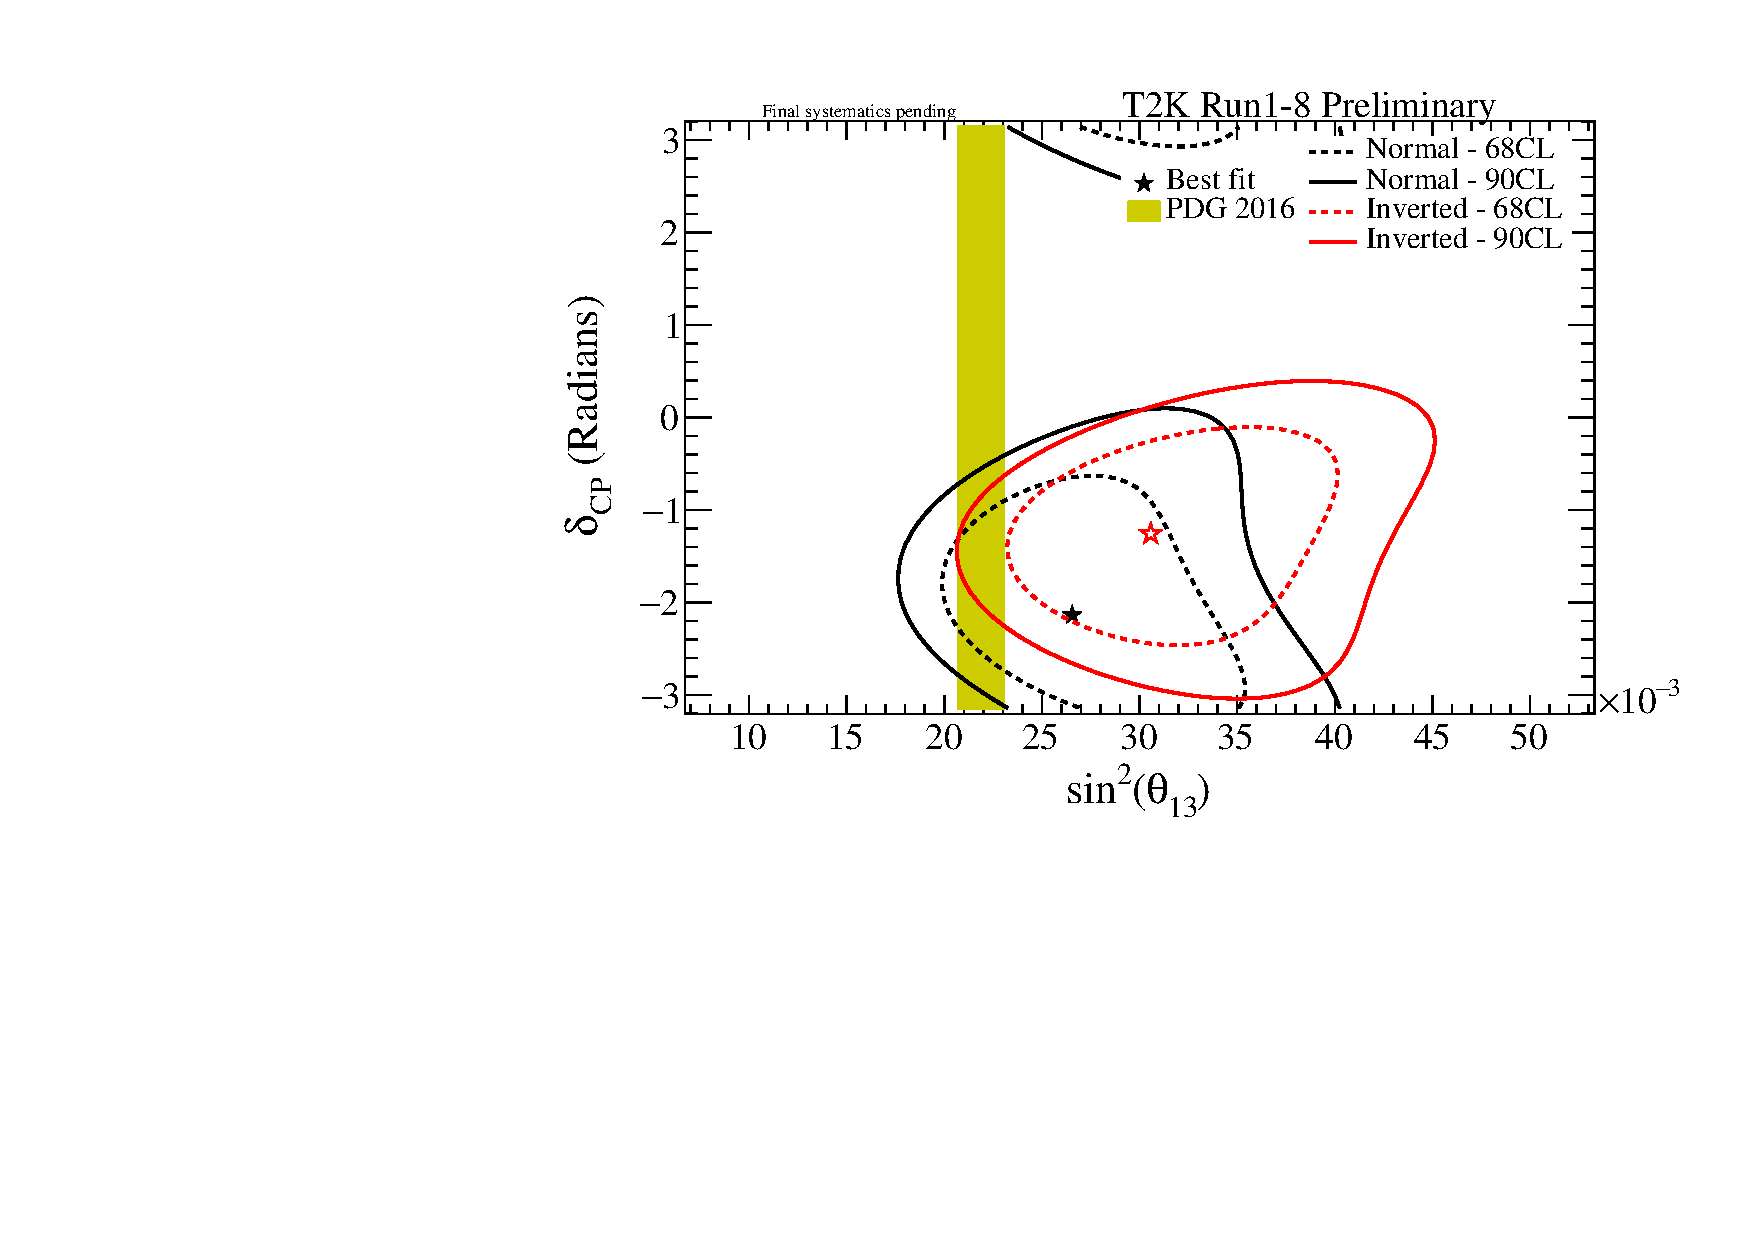
\includegraphics[width=0.9\textwidth]{data/t2k/mixing13_deltacp_data_t2k_global}
		\caption{\appearance T2K only}
	\end{subfigure}
	\caption {
		Contours at 68\% and 90\% CL for \appearance with and without reactor constraint. Normal and inverted hierarchy contours are independent. All 5 samples were used to produce these fits.
	}
	\label{fig:ssqth13_vs_dcp_data}
\end{figure*}

\subsection{Results for \disappearance}

The result for \disappearance with reactor constraint and T2K only is shown in fig.~\ref{fig:ssqth23_vs_dmsq23_data}.

\begin{figure*}[htb]
	\center
	\begin{subfigure}[b]{0.49\textwidth}
		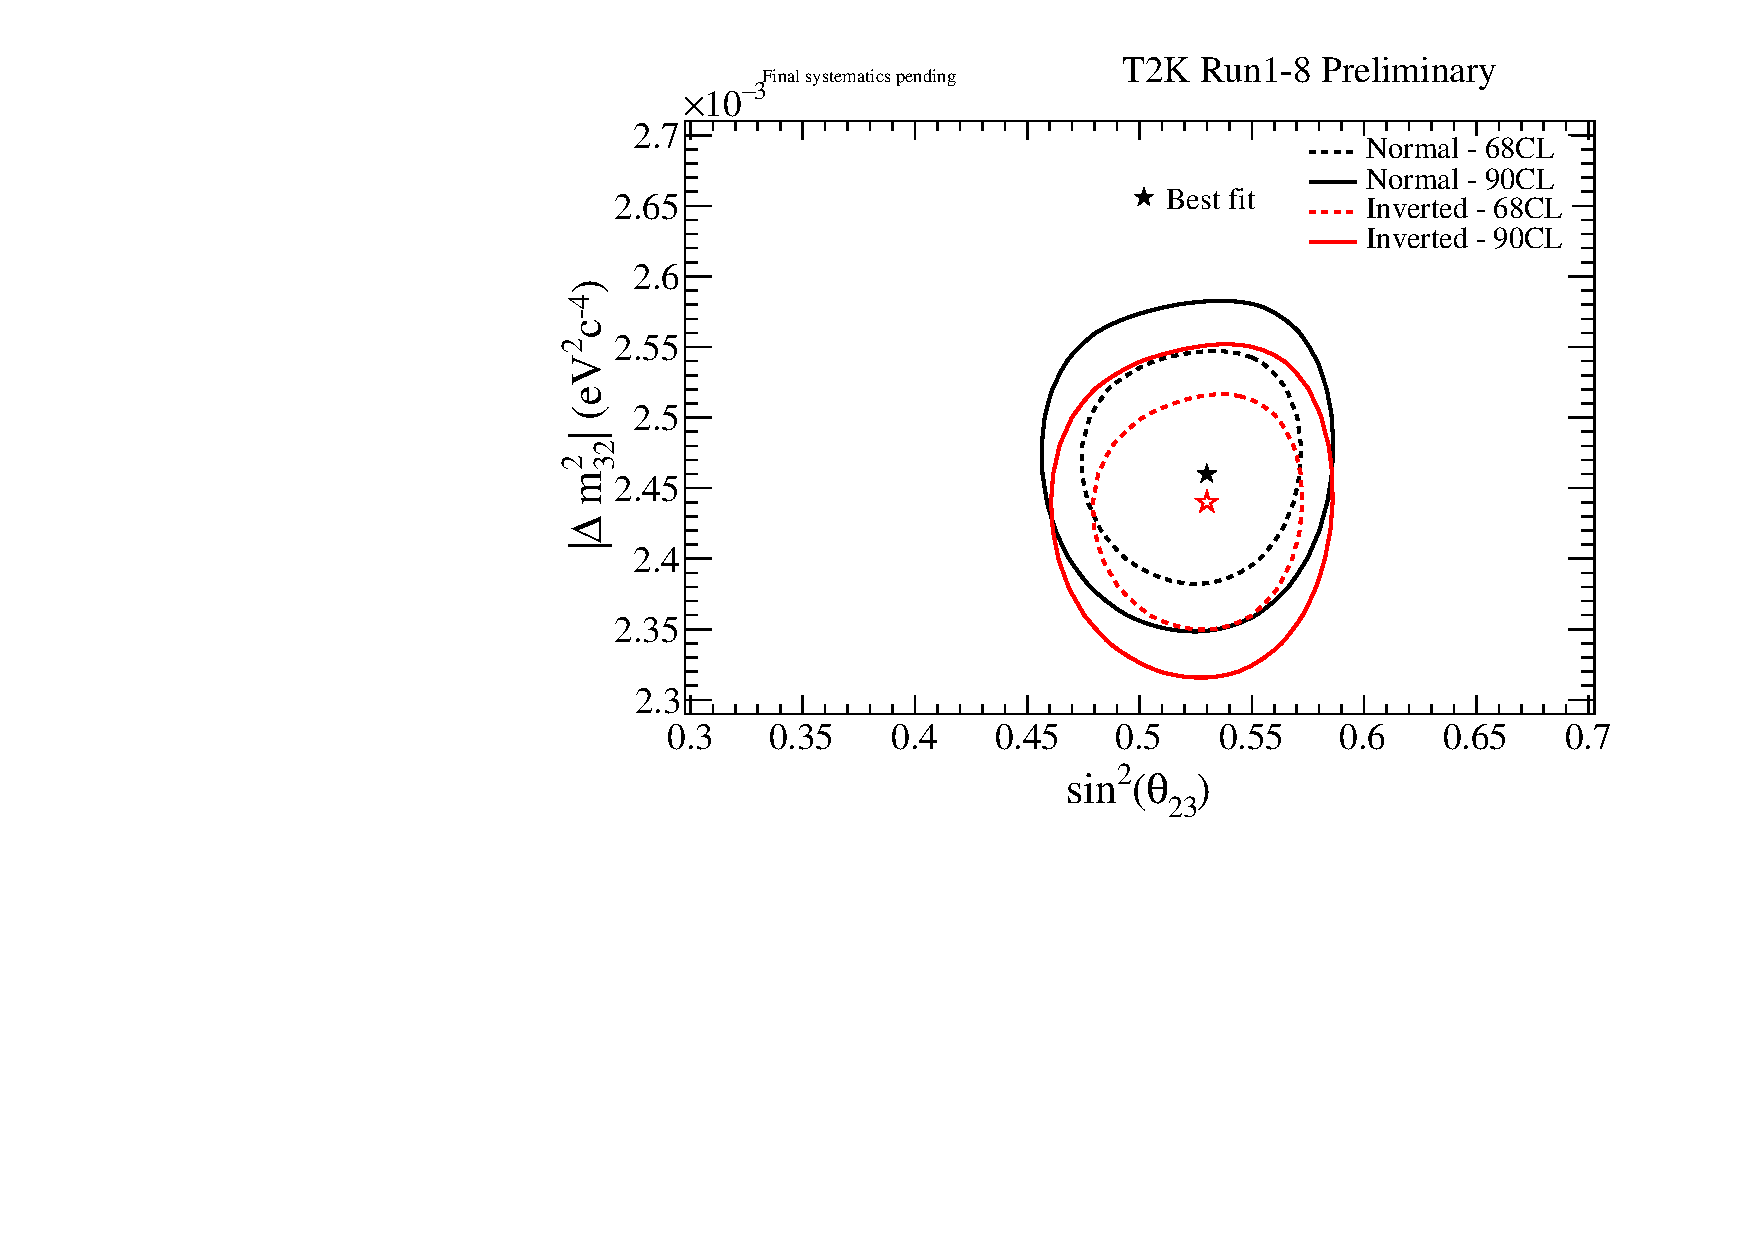
\includegraphics[width=0.9\textwidth]{data/reactor/mixing23_dmsq23_data_reactor_global}
		\caption{\disappearance with reactor constraint}
	\end{subfigure}
	\begin{subfigure}[b]{0.49\textwidth}
		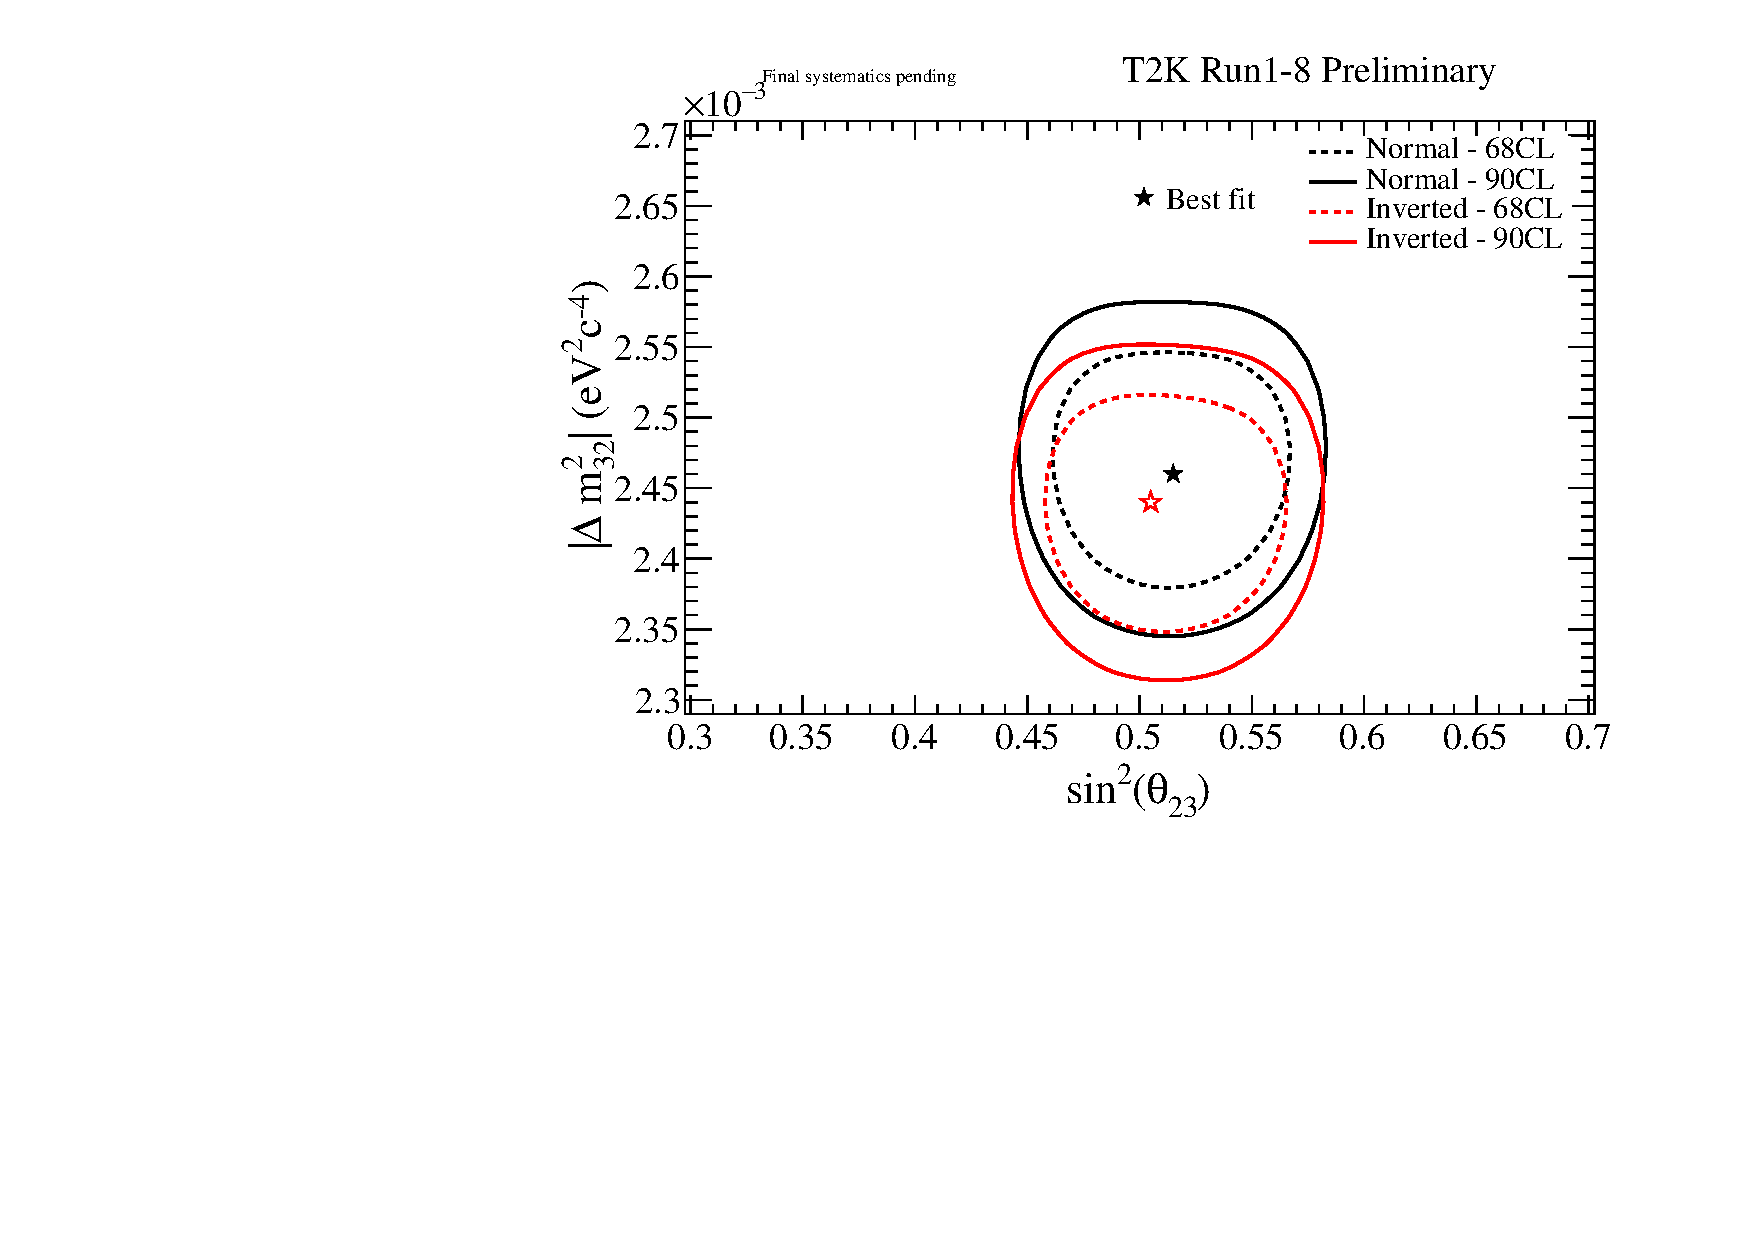
\includegraphics[width=0.9\textwidth]{data/t2k/mixing23_dmsq23_data_t2k_global}
		\caption{\disappearance T2K only}
	\end{subfigure}
	\caption {
		Contours at 68\% and 90\% CL for \disappearance with and without reactor constraint. Normal and inverted hierarchy contours are independent. All 5 samples were used to produce these fits.
	}
	\label{fig:ssqth23_vs_dmsq23_data}
\end{figure*}

\clearpage

\subsection{Results for \deltacp}

The result for \deltacp with reactor constraint and T2K only is shown in fig.~\ref{fig:dcp_data}.

\begin{figure*}[htb]
	\center
	\begin{subfigure}[b]{0.49\textwidth}
		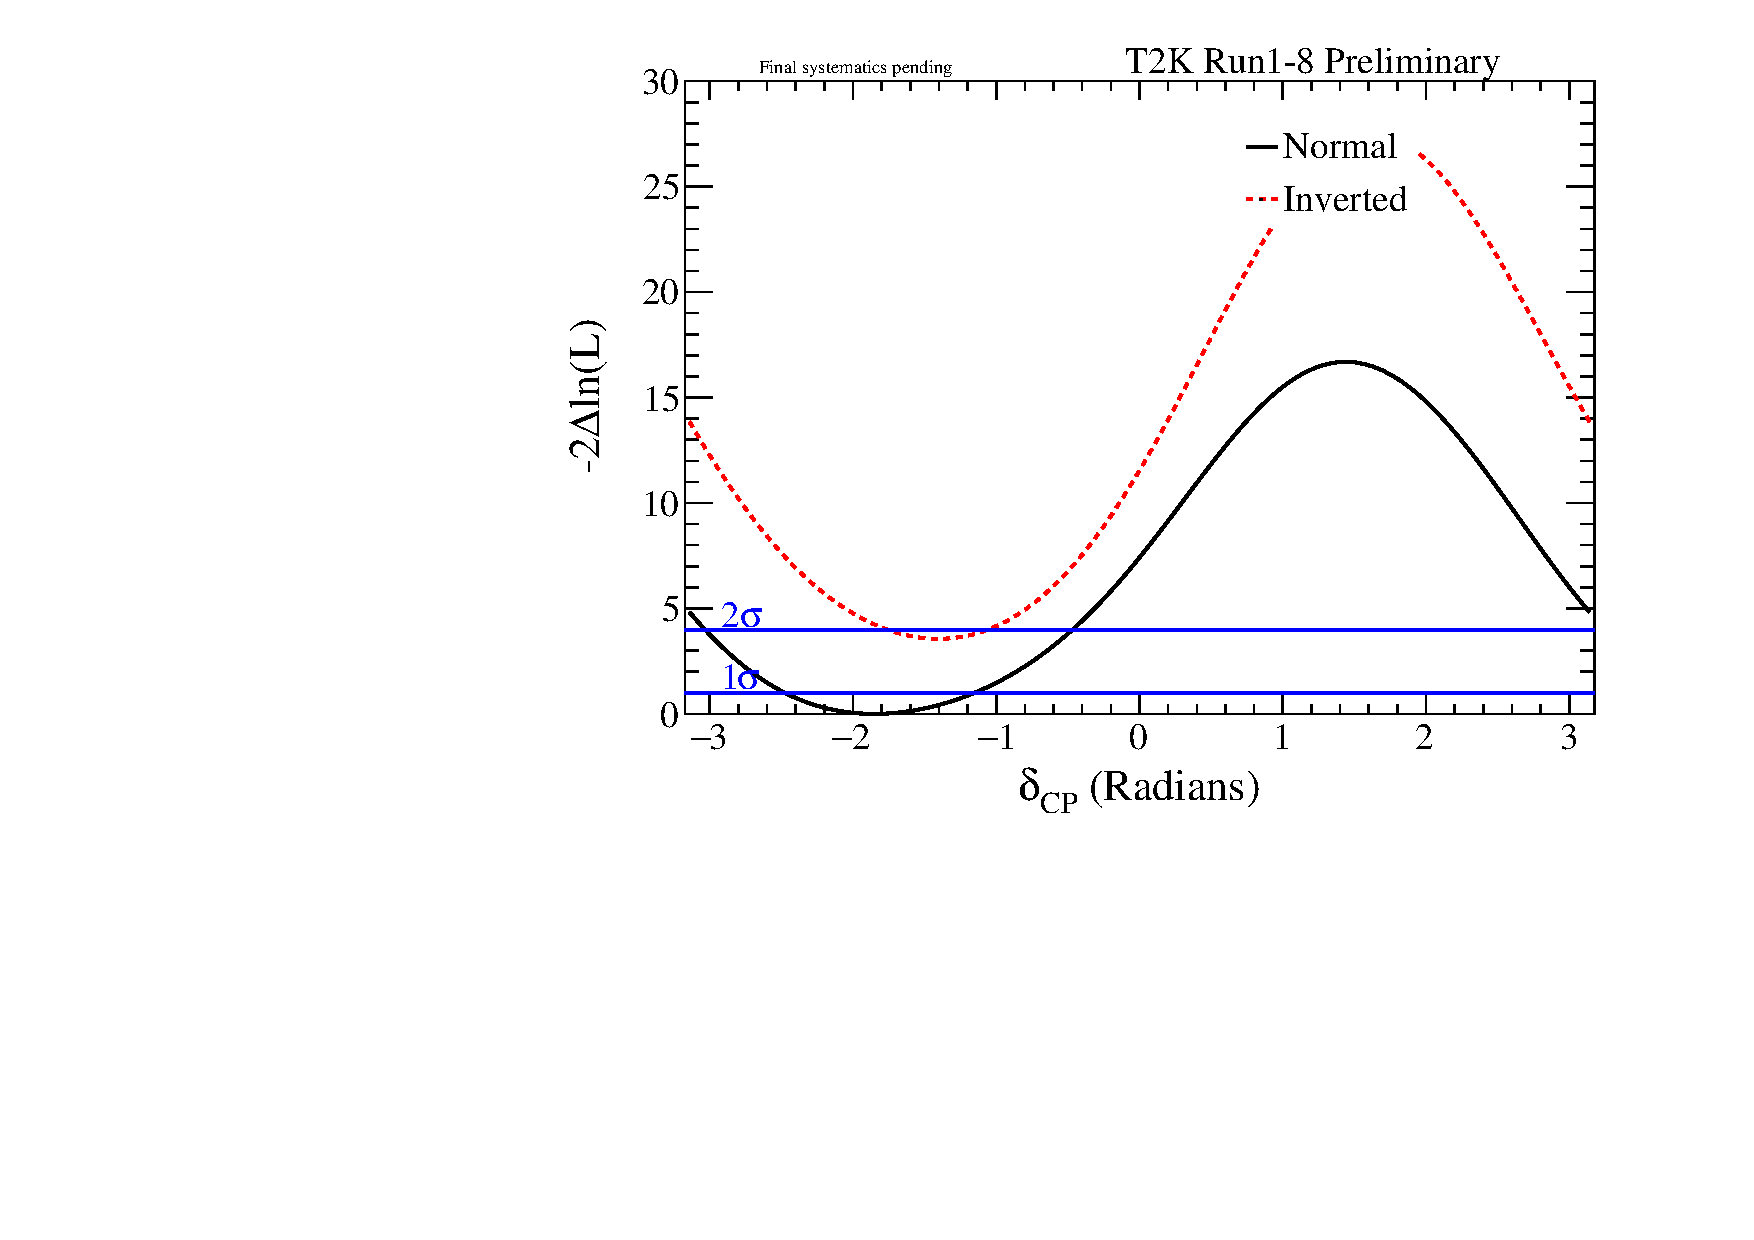
\includegraphics[width=0.9\textwidth]{data/reactor/deltacp_data_reactor_global}
		\caption{\deltacp with reactor constraint}
	\end{subfigure}
	\begin{subfigure}[b]{0.49\textwidth}
		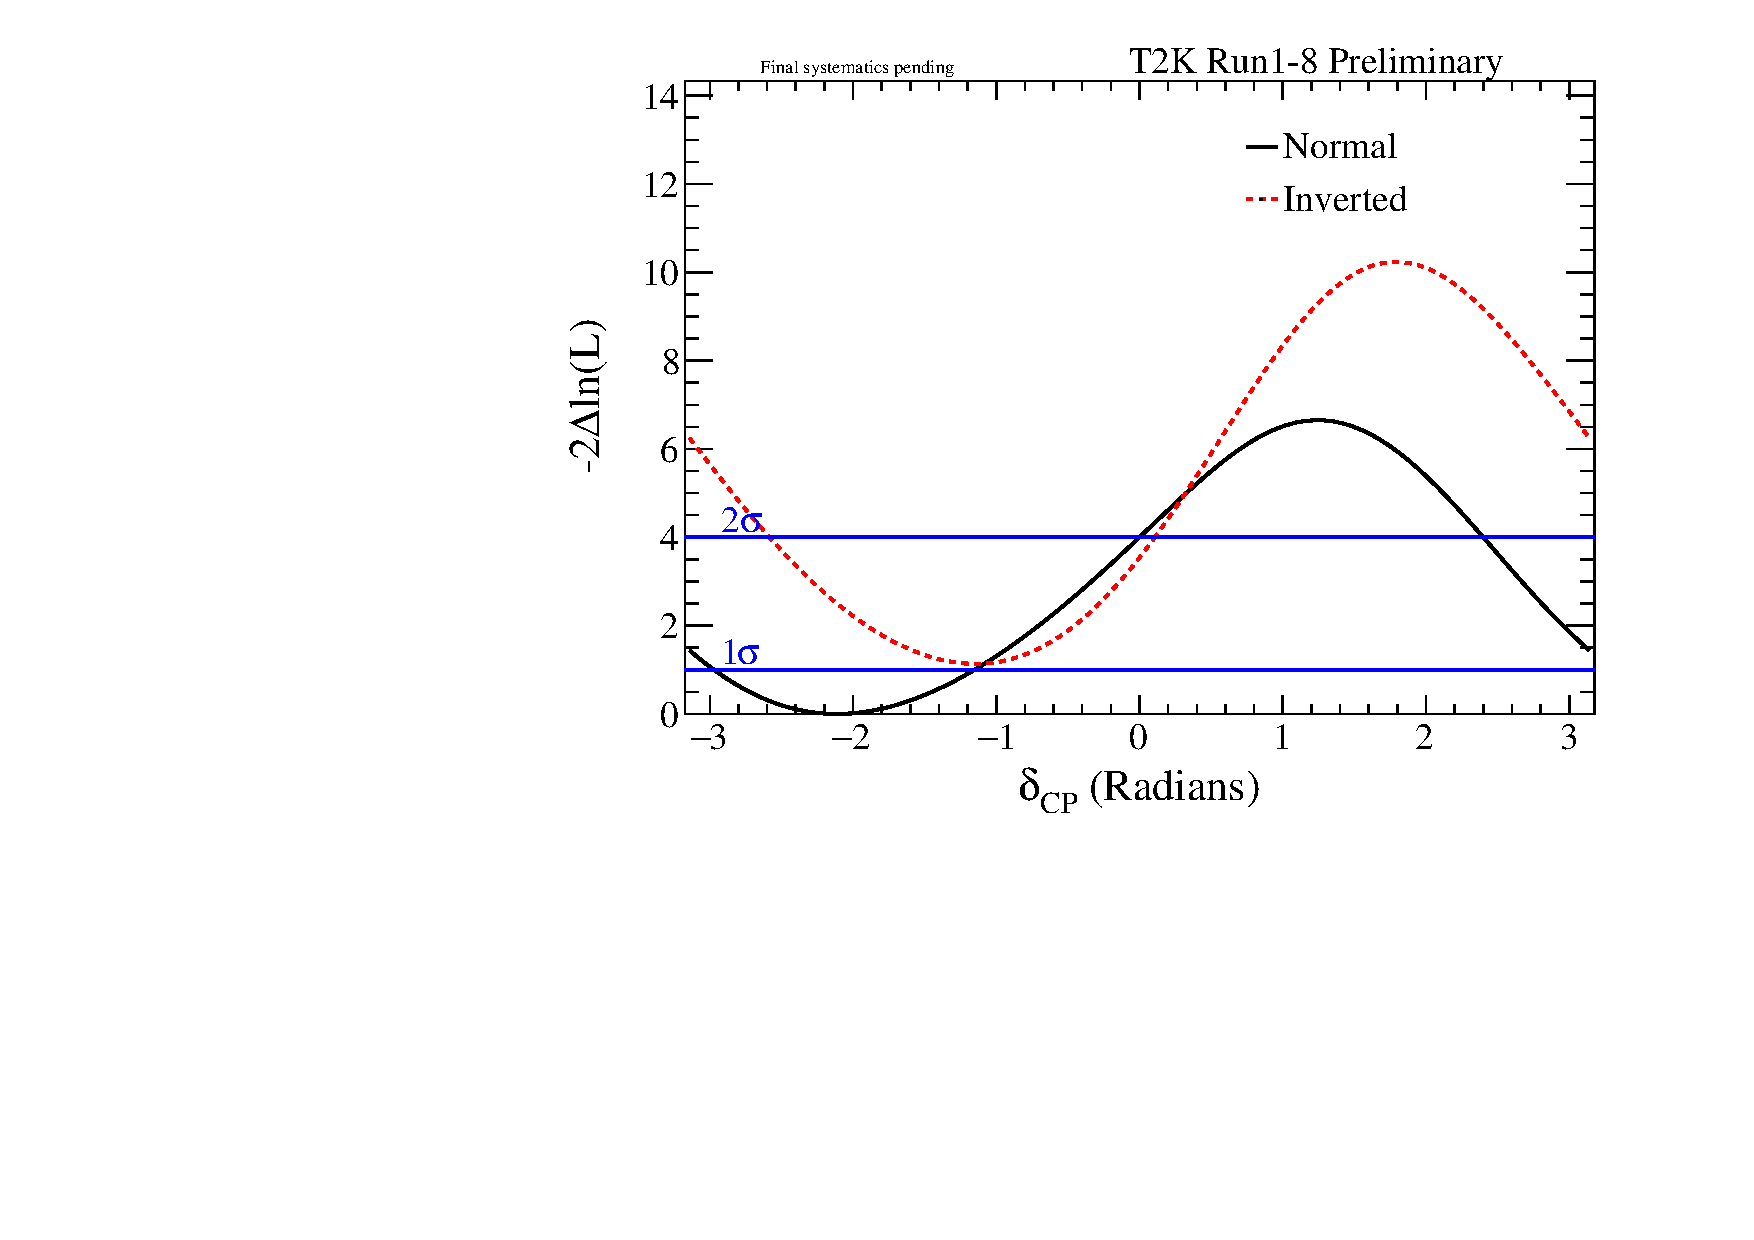
\includegraphics[width=0.9\textwidth]{data/t2k/deltacp_data_t2k_global}
		\caption{\deltacp T2K only}
	\end{subfigure}
	\caption {
		The expected $\Delta\chi^2$ distribution as a function of \deltacp with and without reactor constraint. The mass hierarchy is minimized, with normal and inverted hierarchy $\Delta\chi^2$ distributions shifted to the same global best-fit $\chi^2$ value, which is taken to be the minimum between normal and inverted hierarchy. All 5 samples were used to produce these fits.
	}
	\label{fig:dcp_data}
\end{figure*}

\subsection{Results for \ssqthonethree}

The result for \ssqthonethree (without reactor constraint) is shown in fig.~\ref{fig:th13_data}.

\begin{figure*}[htb]
	\center
	\begin{subfigure}[b]{0.49\textwidth}
		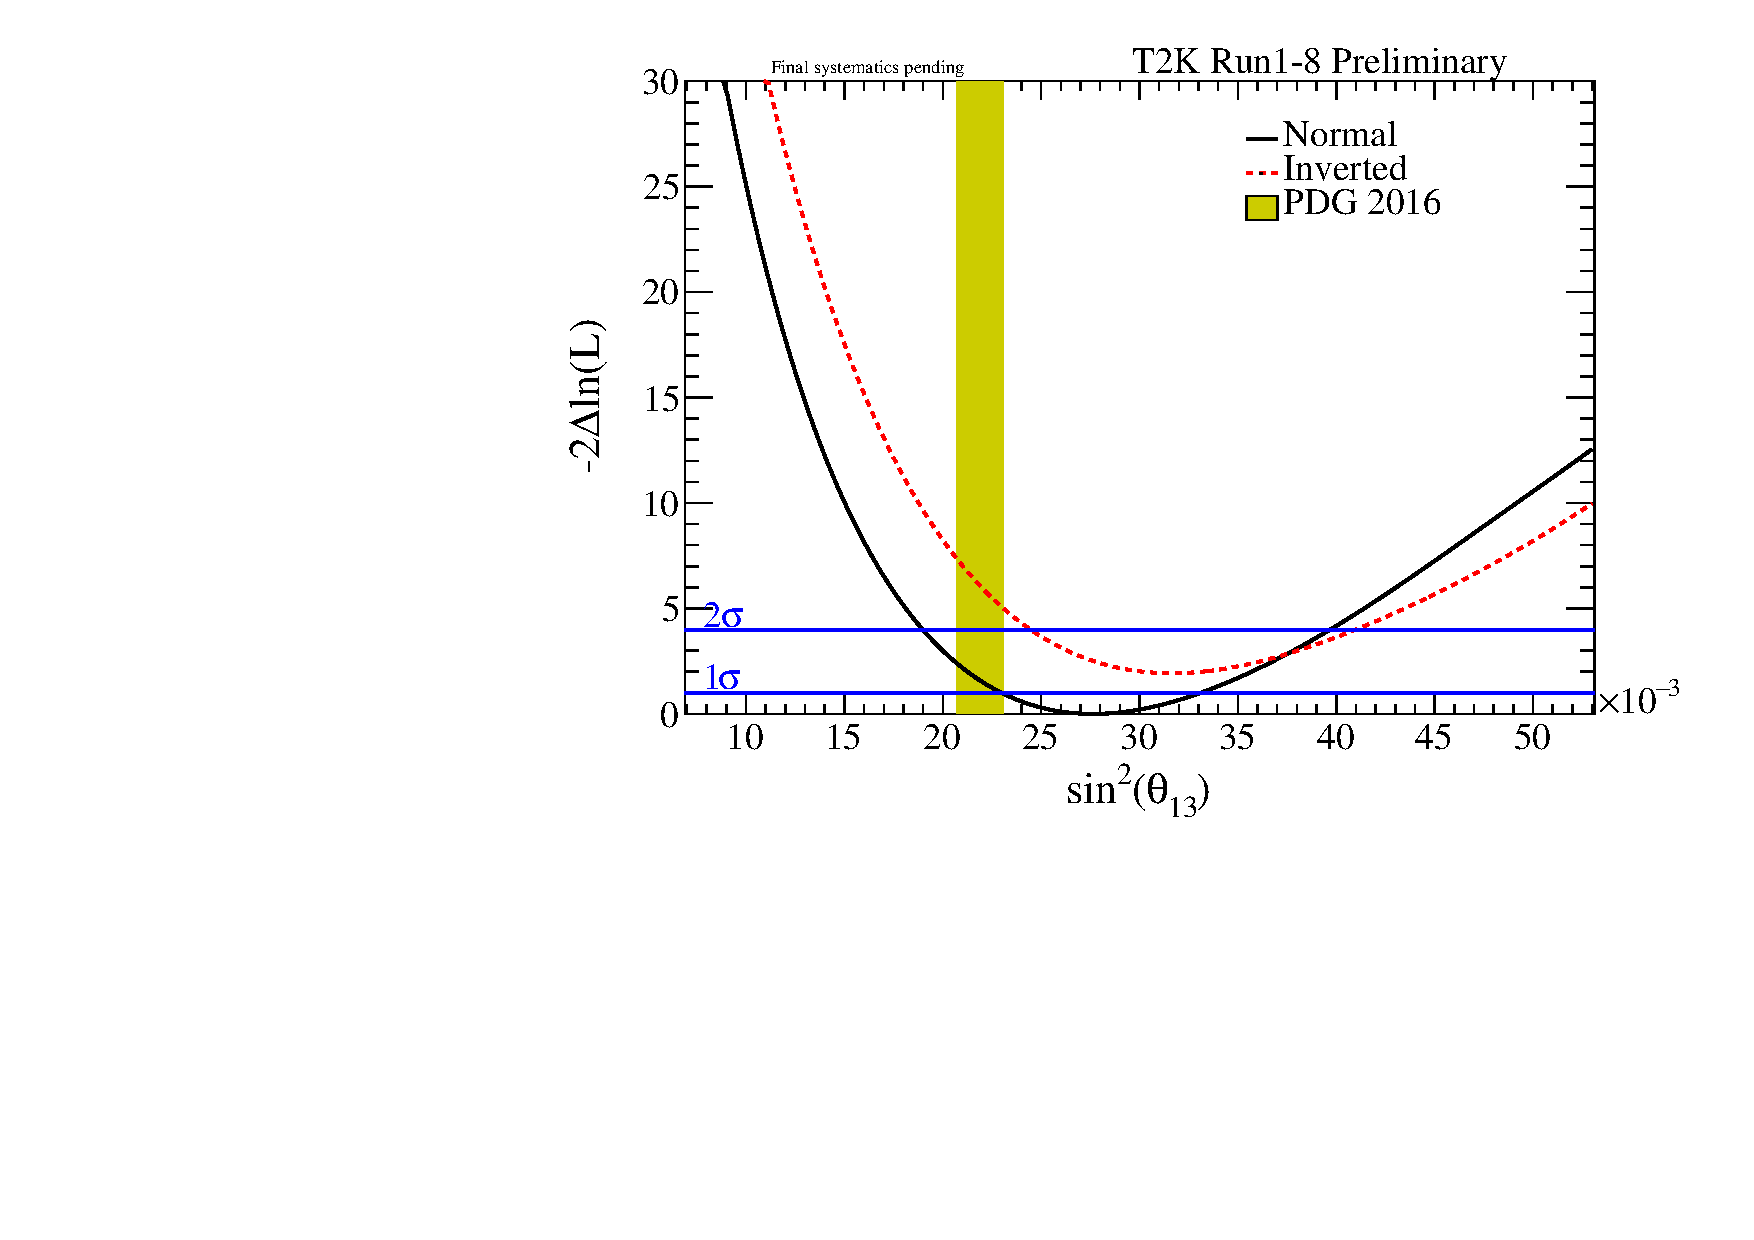
\includegraphics[width=0.9\textwidth]{data/t2k/mixing13_data_t2k_global}
		\caption{\ssqthonethree T2K only}
	\end{subfigure}
	\caption {
		The expected $\Delta\chi^2$ distribution as a function of \ssqthonethree without reactor constraint. The mass hierarchy is minimized, with normal and inverted hierarchy $\Delta\chi^2$ distributions shifted to the same global best-fit $\chi^2$ value, which is taken to be the minimum between normal and inverted hierarchy. All 5 samples were used to produce these fits.
	}
	\label{fig:th13_data}
\end{figure*}

\clearpage

\subsection{Results for \ssqthtwothree}

The result for \ssqthtwothree with reactor constraint and T2K only is shown in fig.~\ref{fig:th23_data}.

\begin{figure*}[htb]
	\center
	\begin{subfigure}[b]{0.49\textwidth}
		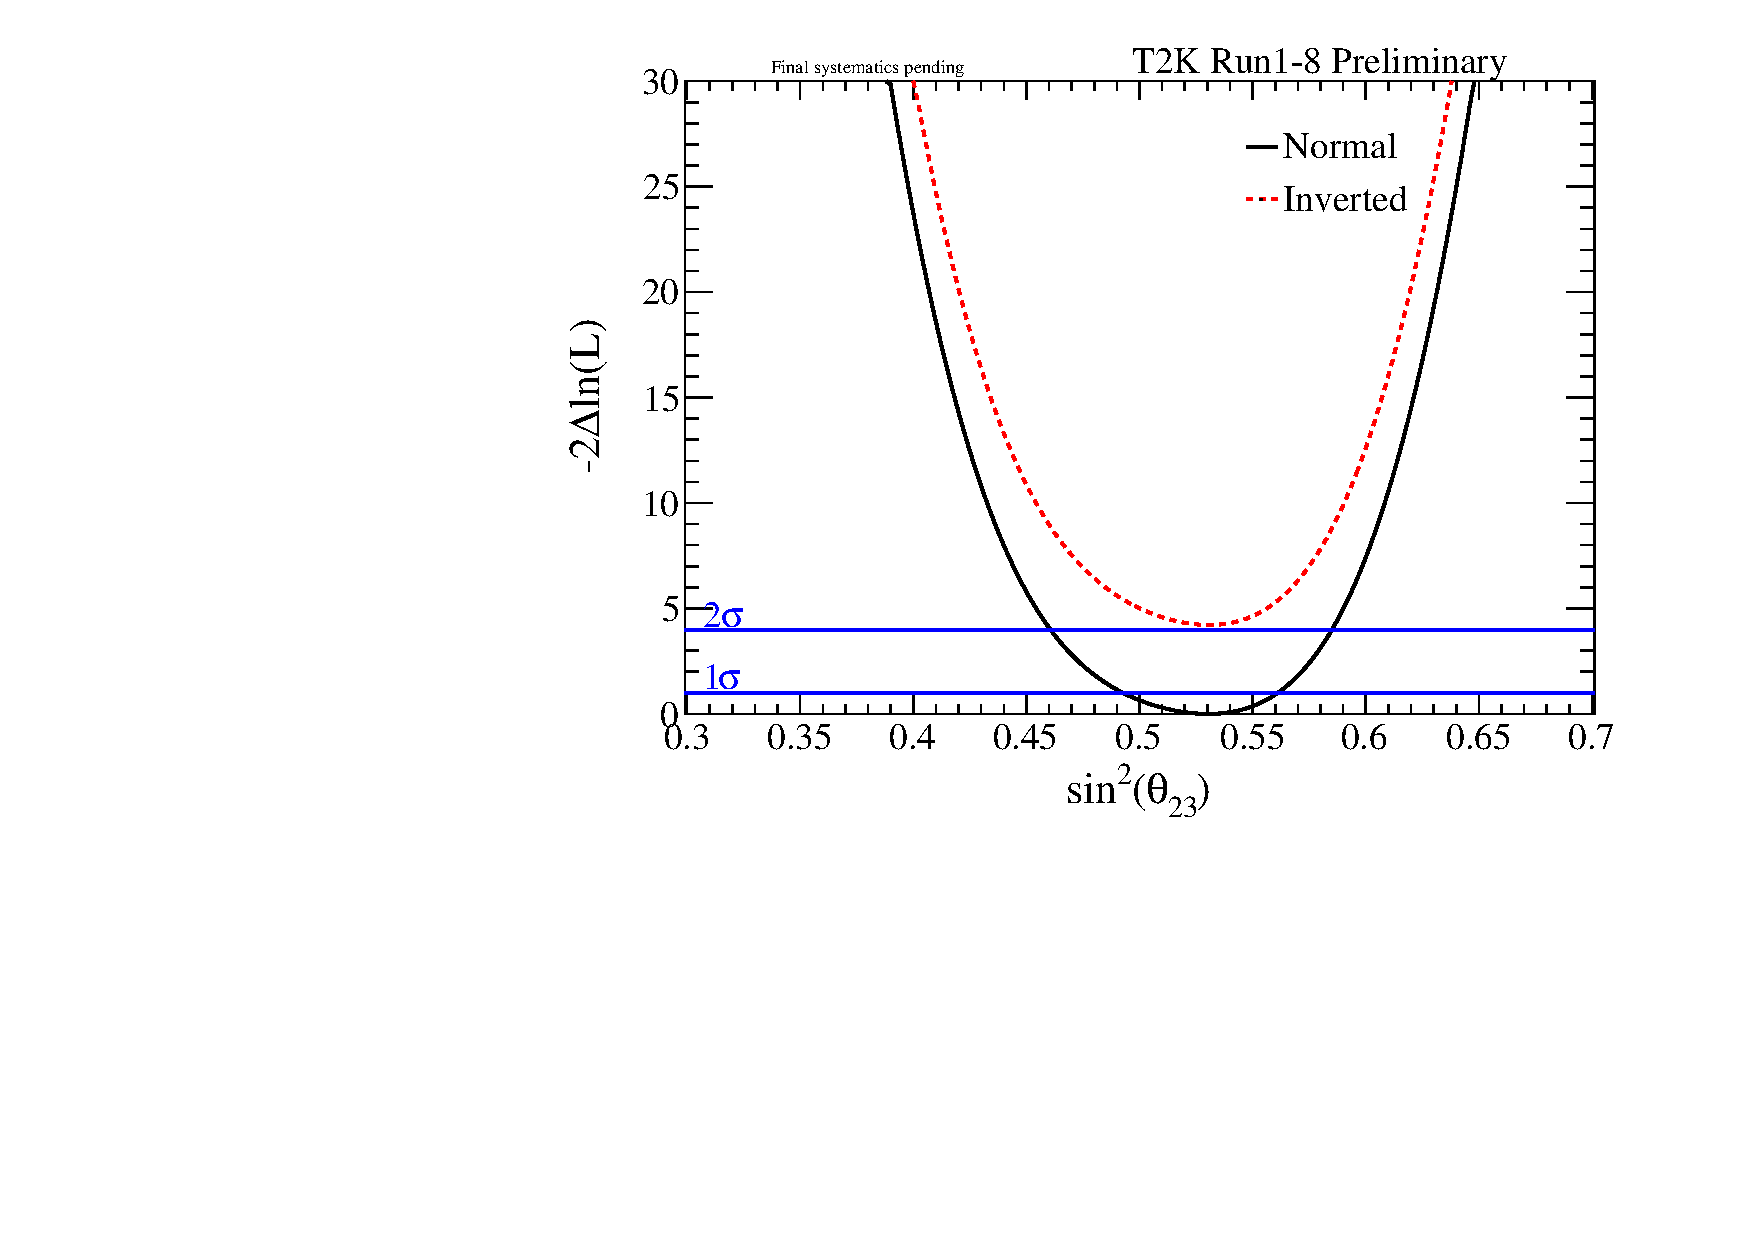
\includegraphics[width=0.9\textwidth]{data/reactor/mixing23_data_reactor_global}
		\caption{\ssqthtwothree with reactor constraint}
	\end{subfigure}
	\begin{subfigure}[b]{0.49\textwidth}
		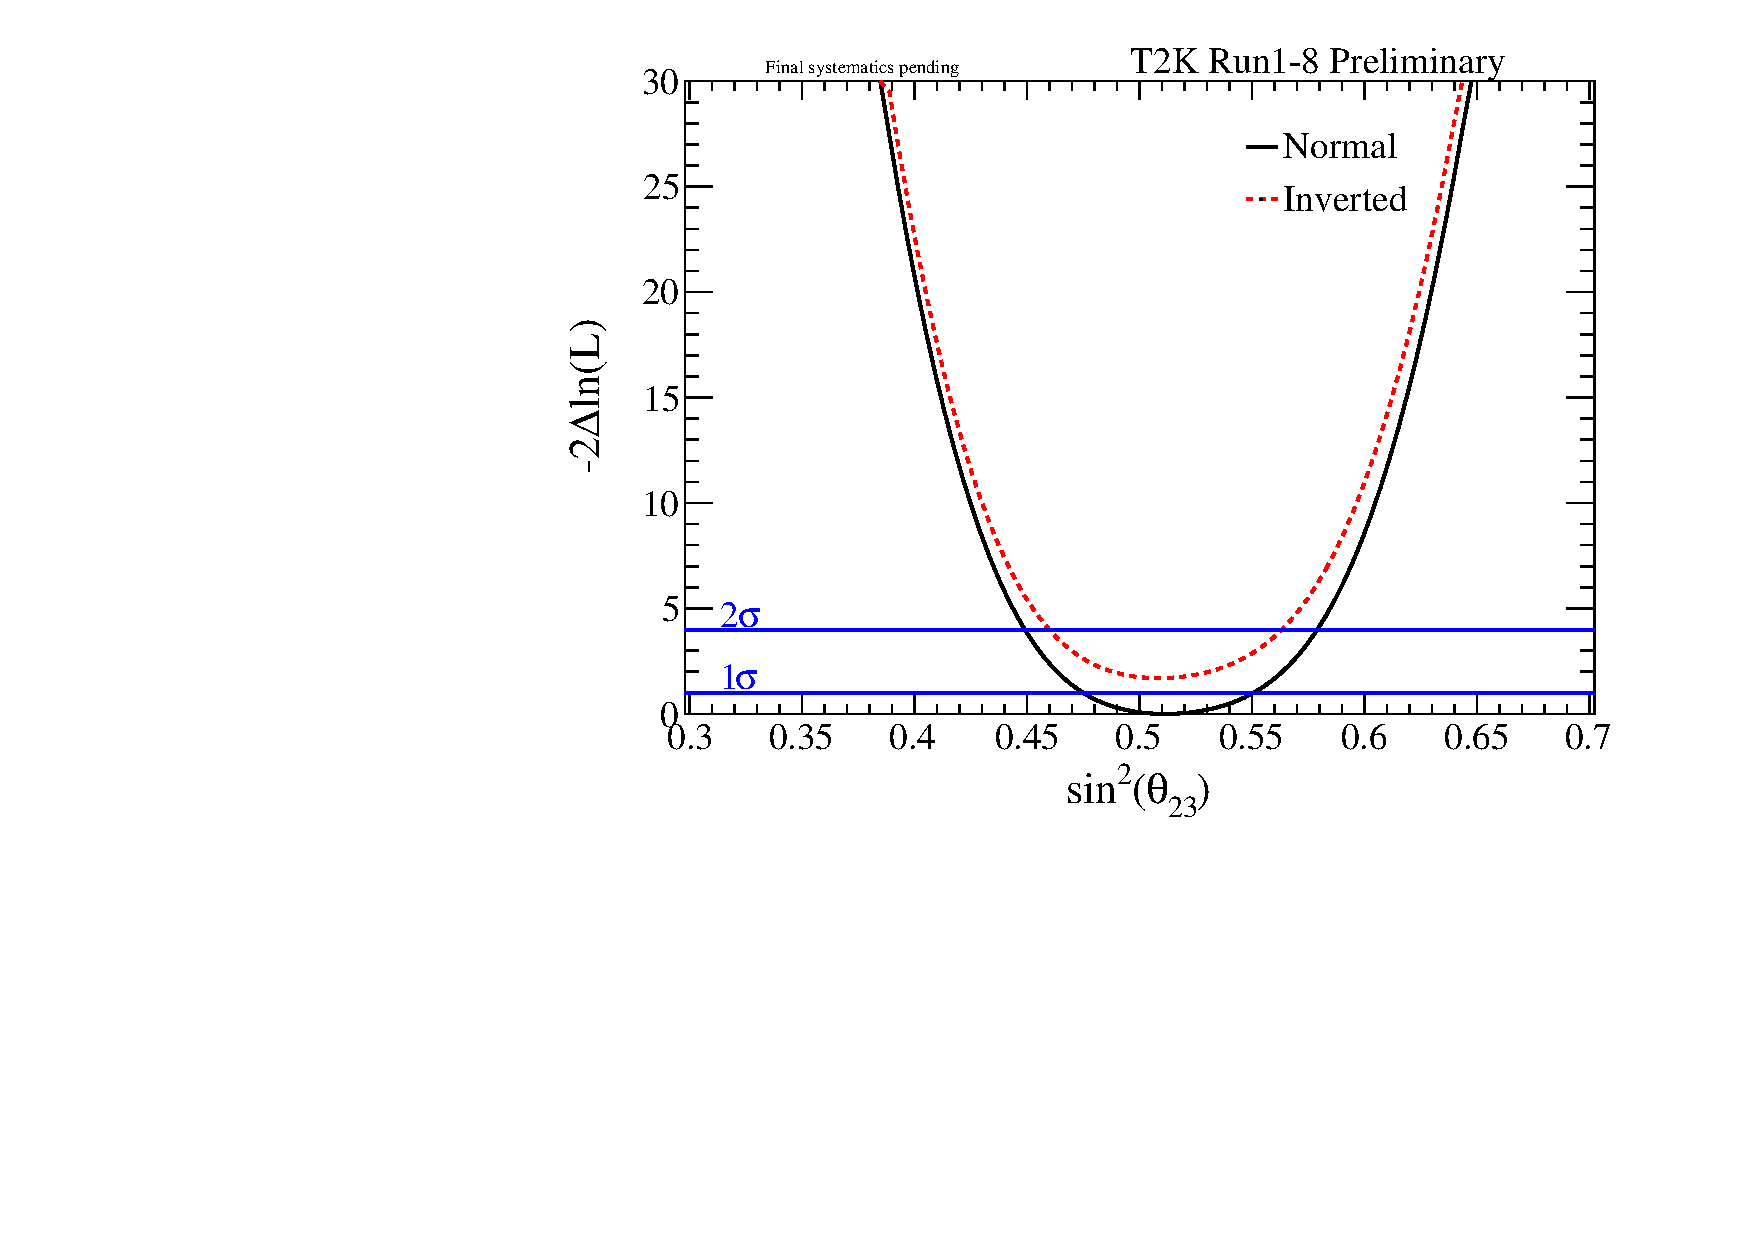
\includegraphics[width=0.9\textwidth]{data/t2k/mixing23_data_t2k_global}
		\caption{\ssqthtwothree T2K only}
	\end{subfigure}
	\caption {
		The expected $\Delta\chi^2$ distribution as a function of \ssqthtwothree with and without reactor constraint. The mass hierarchy is minimized, with normal and inverted hierarchy $\Delta\chi^2$ distributions shifted to the same global best-fit $\chi^2$ value, which is taken to be the minimum between normal and inverted hierarchy. All 5 samples were used to produce these fits.
	}
	\label{fig:th23_data}
\end{figure*}

\subsection{Results for \dmsqtwothree}

The result for \dmsqtwothree with reactor constraint and T2K only is shown in fig.~\ref{fig:dmsq23_data}.

\begin{figure*}[htb]
	\center
	\begin{subfigure}[b]{0.49\textwidth}
		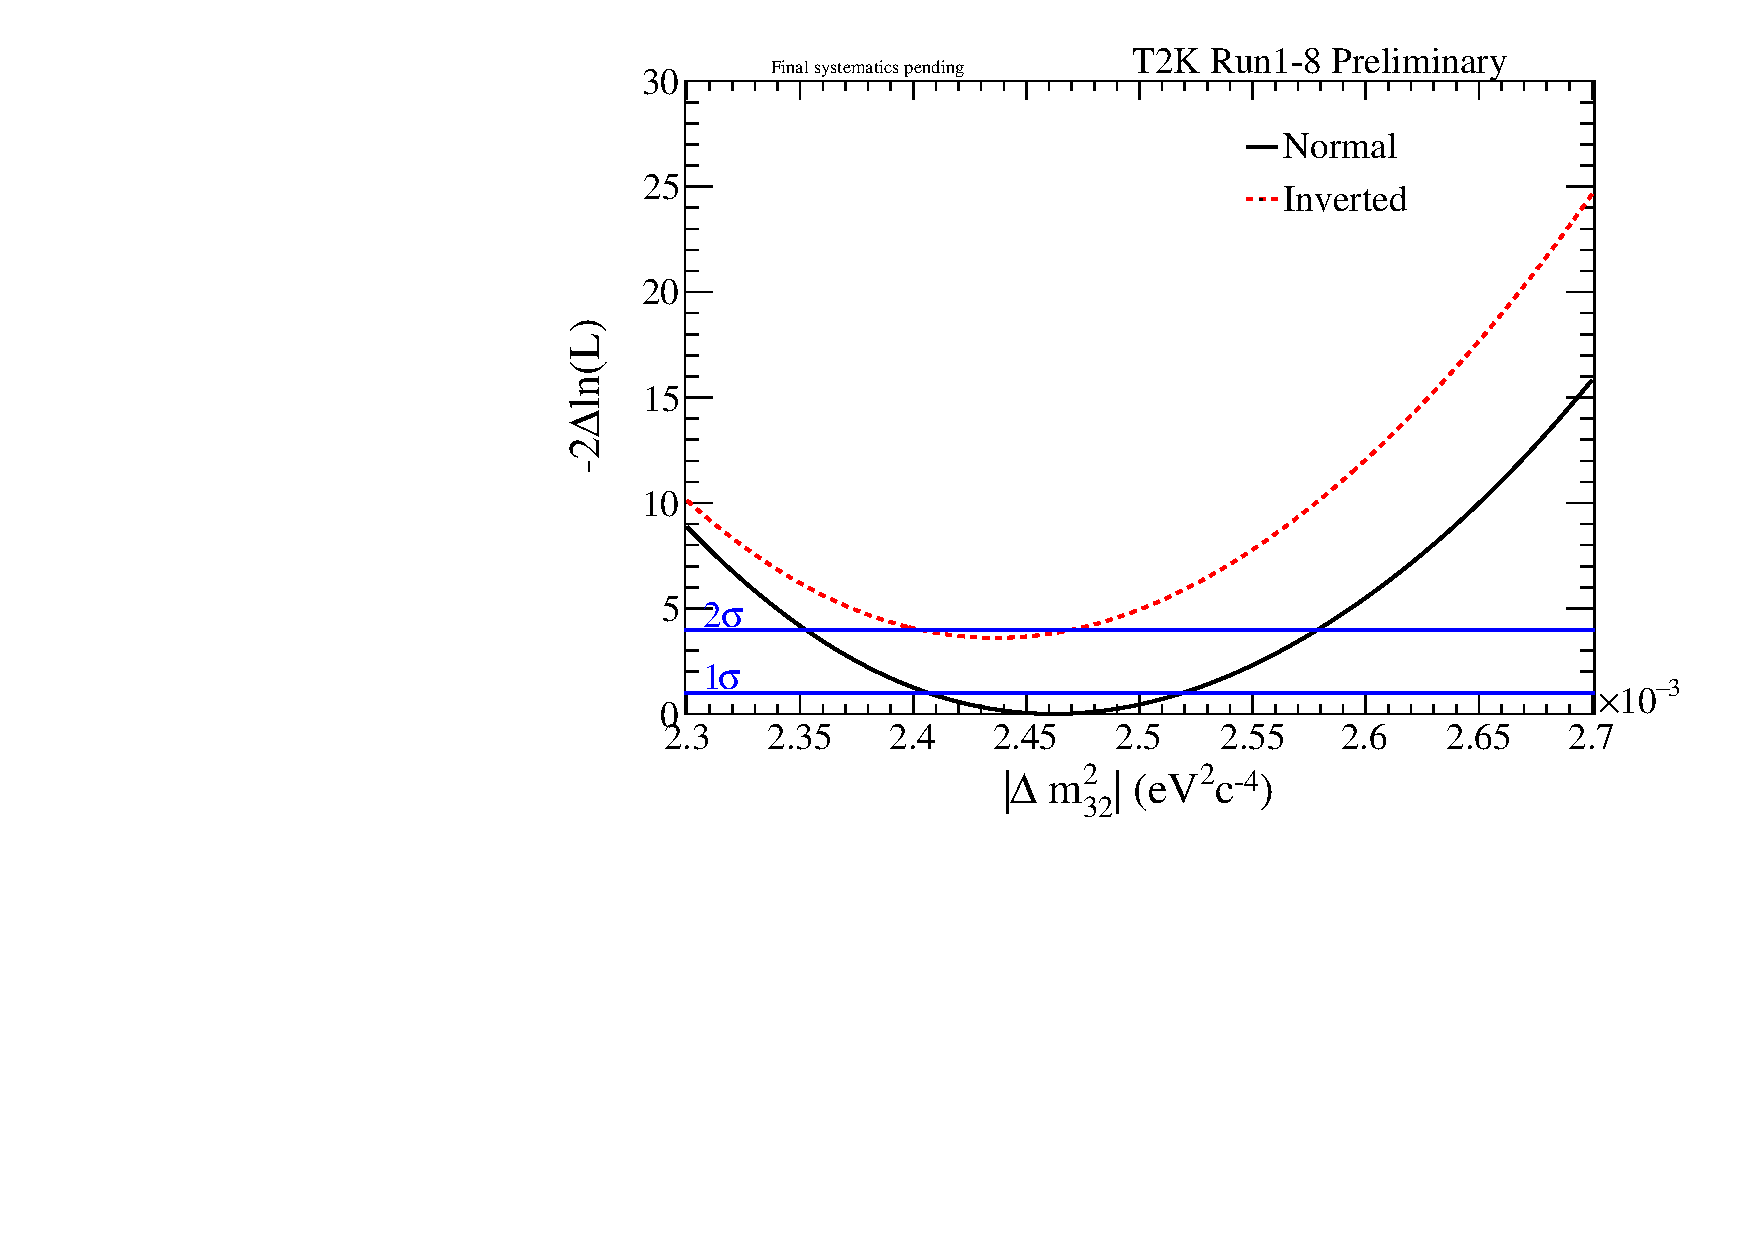
\includegraphics[width=0.9\textwidth]{data/reactor/dmsq23_data_reactor_global}
		\caption{\dmsqtwothree with reactor constraint}
	\end{subfigure}
	\begin{subfigure}[b]{0.49\textwidth}
		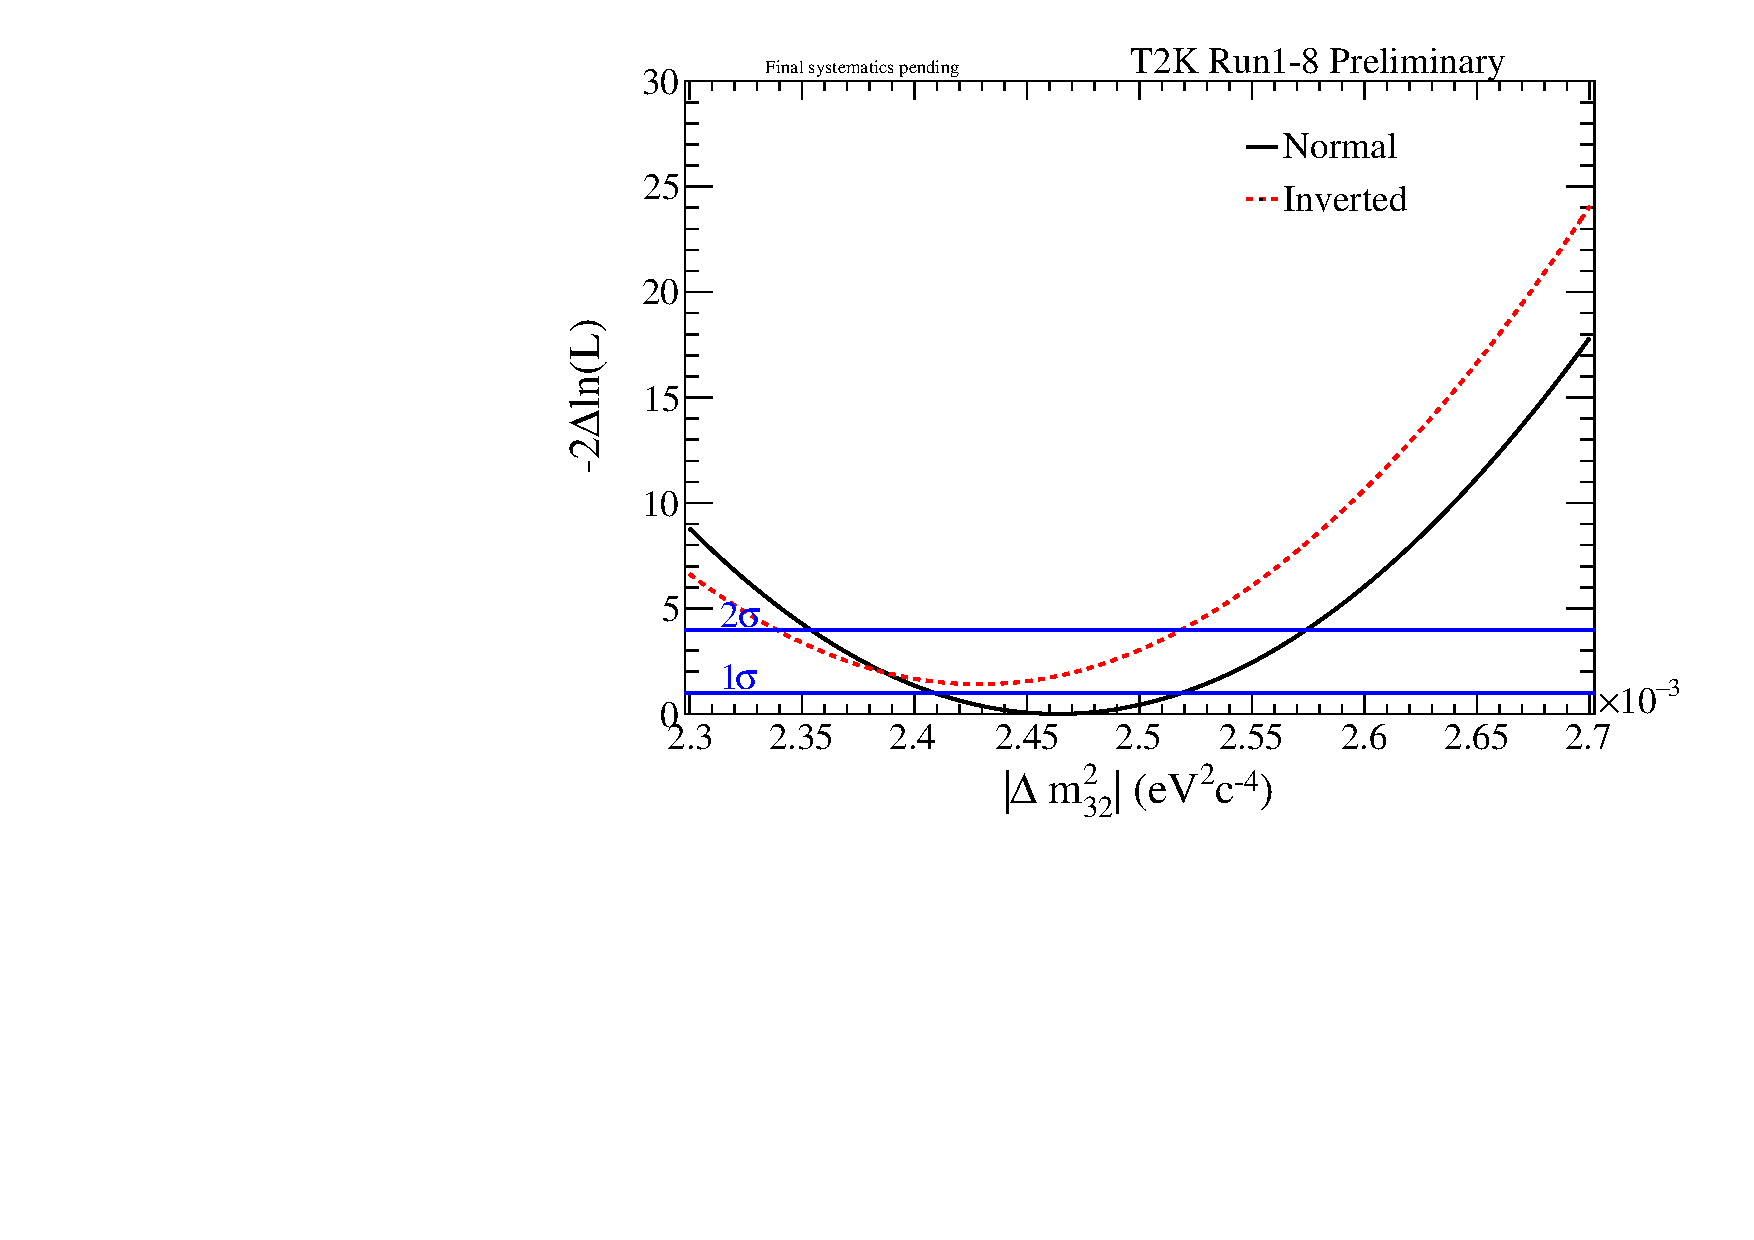
\includegraphics[width=0.9\textwidth]{data/t2k/dmsq23_data_t2k_global}
		\caption{\dmsqtwothree T2K only}
	\end{subfigure}
	\caption {
		The expected $\Delta\chi^2$ distribution as a function of \dmsqtwothree with and without reactor constraint. The mass hierarchy is minimized, with normal and inverted hierarchy $\Delta\chi^2$ distributions shifted to the same global best-fit $\chi^2$ value, which is taken to be the minimum between normal and inverted hierarchy. All 5 samples were used to produce these fits.
	}
	\label{fig:dmsq23_data}
\end{figure*}

\subsection {Feldman-Cousins simultaneous fit of \deltacp and mass hierarchy}
\label{sec:fc_significance}


This section presents the results of the Feldman-Cousins fit of \deltacp and mass hierarchy. Throws of oscillation parameters are made according to PDG 2016 best-fit values and errors for \ssqthonethree, \ssqthonetwo and \dmsqonetwo, whilst \ssqthtwothree and \dmsqtwothree are thrown according to the likelihood distribution produced by an Asimov fit using the best-fit from data for these parameters, this is an updated method from the previous analysis and the proposal is given in \cite{NewFC}. \deltacp is fixed at one of 9 evenly specified values on the range $\left[-\pi,\pi\right]$.

\subsubsection{Input oscillation parameters}
\label{sec:fc_significance:inputs}

The distributions of oscillation parameters (for normal hierarchy) are shown in \cref{fig:fc_input_dist}. Note that whilst the distributions of the atmospheric parameters are shown independently they are generated jointly from the likelihood distribution shown in \cref{fig:fc_input_disapp}.

\begin{figure*}[htb]
	\center
	\begin{subfigure}[b]{0.49\textwidth}
		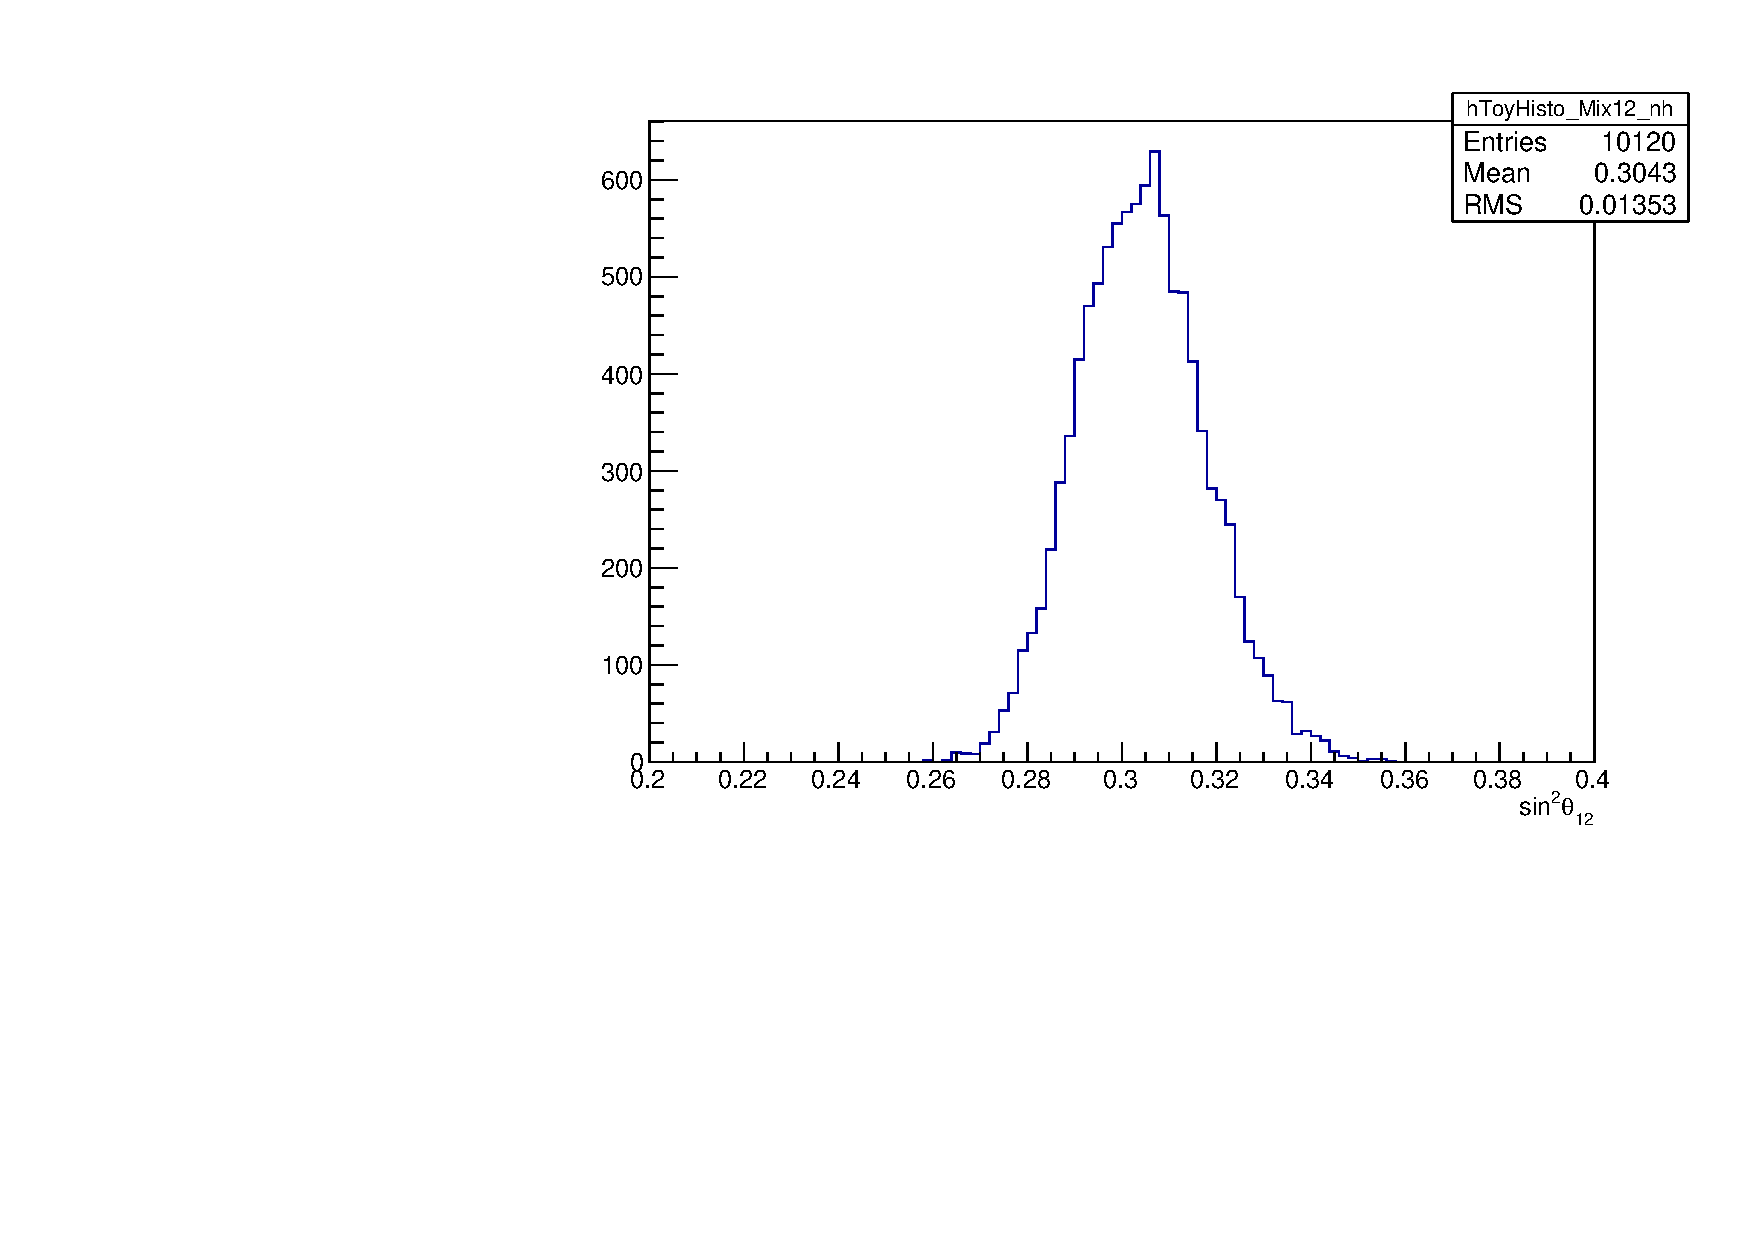
\includegraphics[width=0.9\textwidth]{data/fc/inputs/mixing12_in}
		\caption{\ssqthonetwo}
	\end{subfigure}
	\begin{subfigure}[b]{0.49\textwidth}
		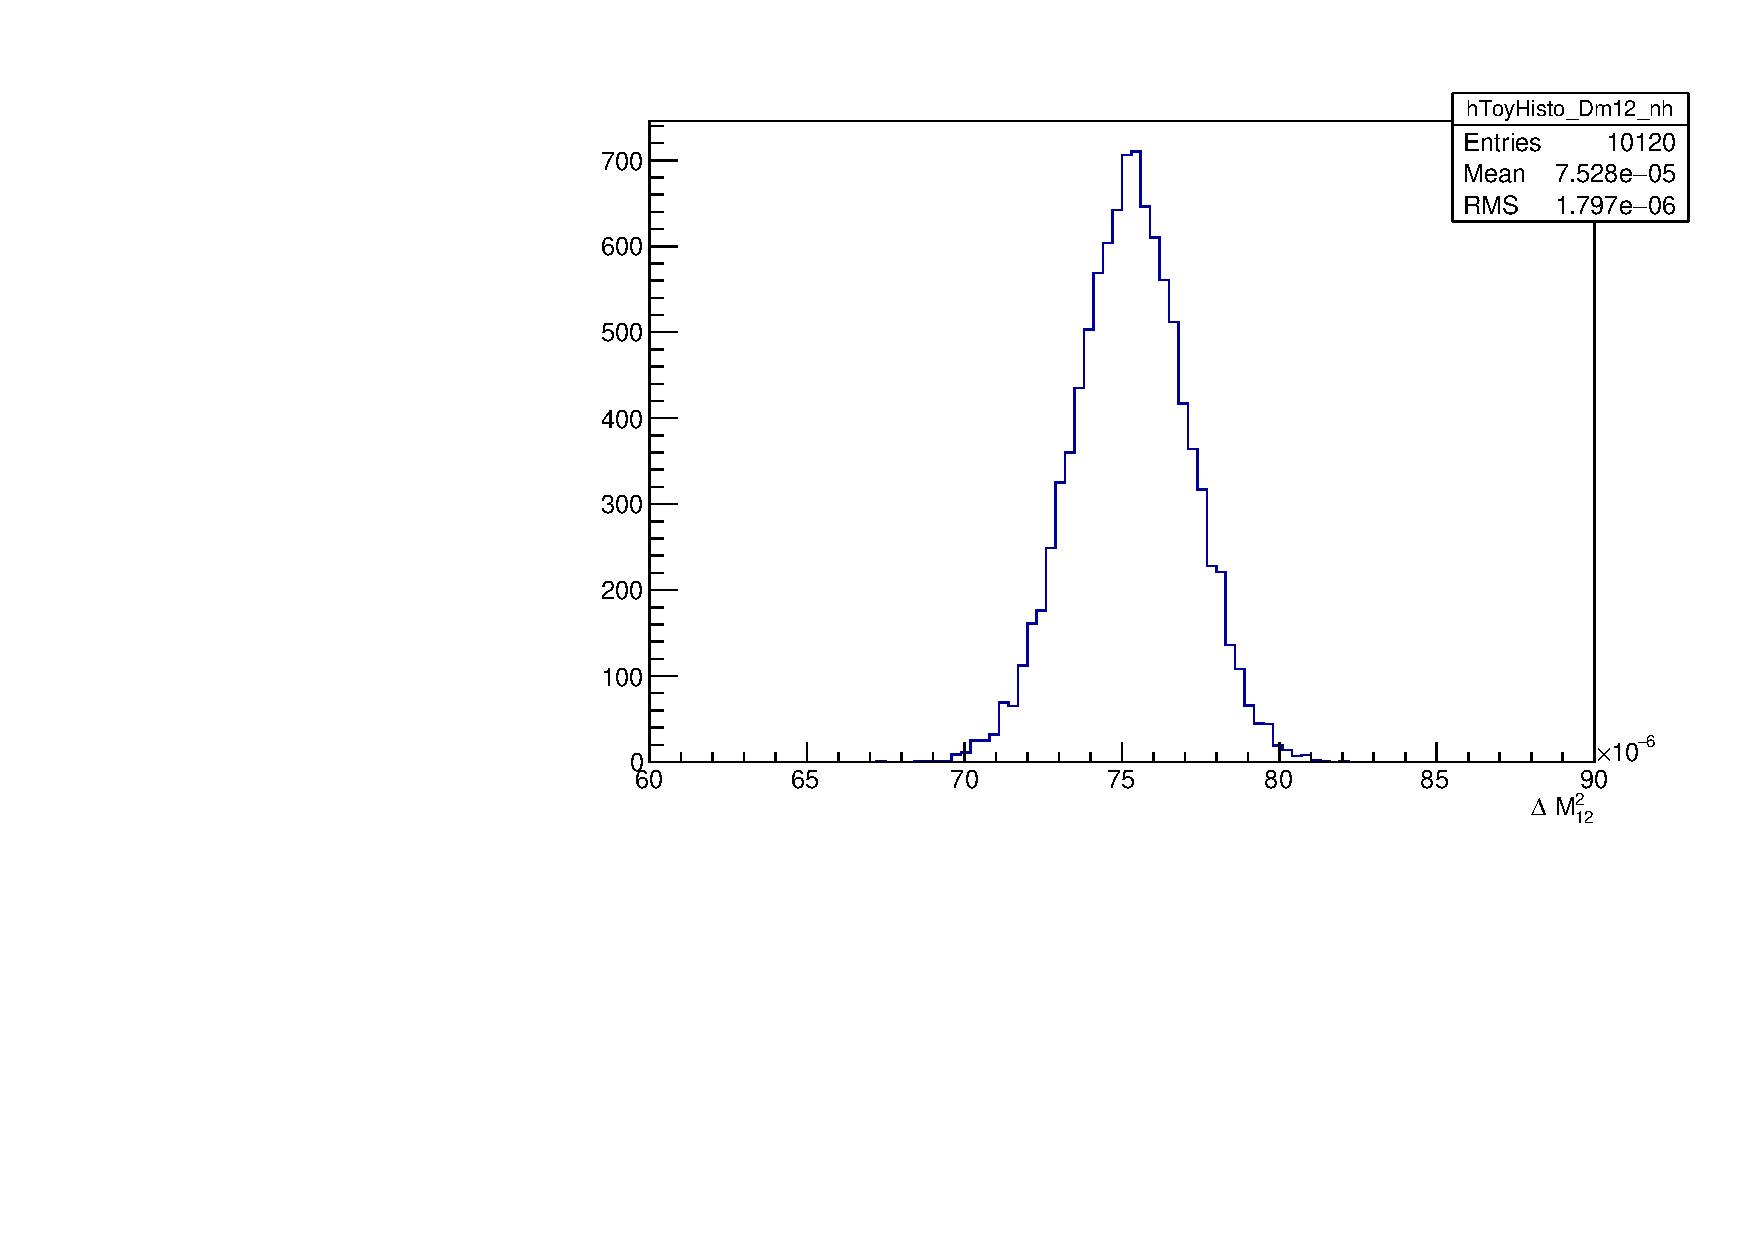
\includegraphics[width=0.9\textwidth]{data/fc/inputs/dm12_in}
		\caption{\dmsqonetwo}
	\end{subfigure}
	\begin{subfigure}[b]{0.49\textwidth}
		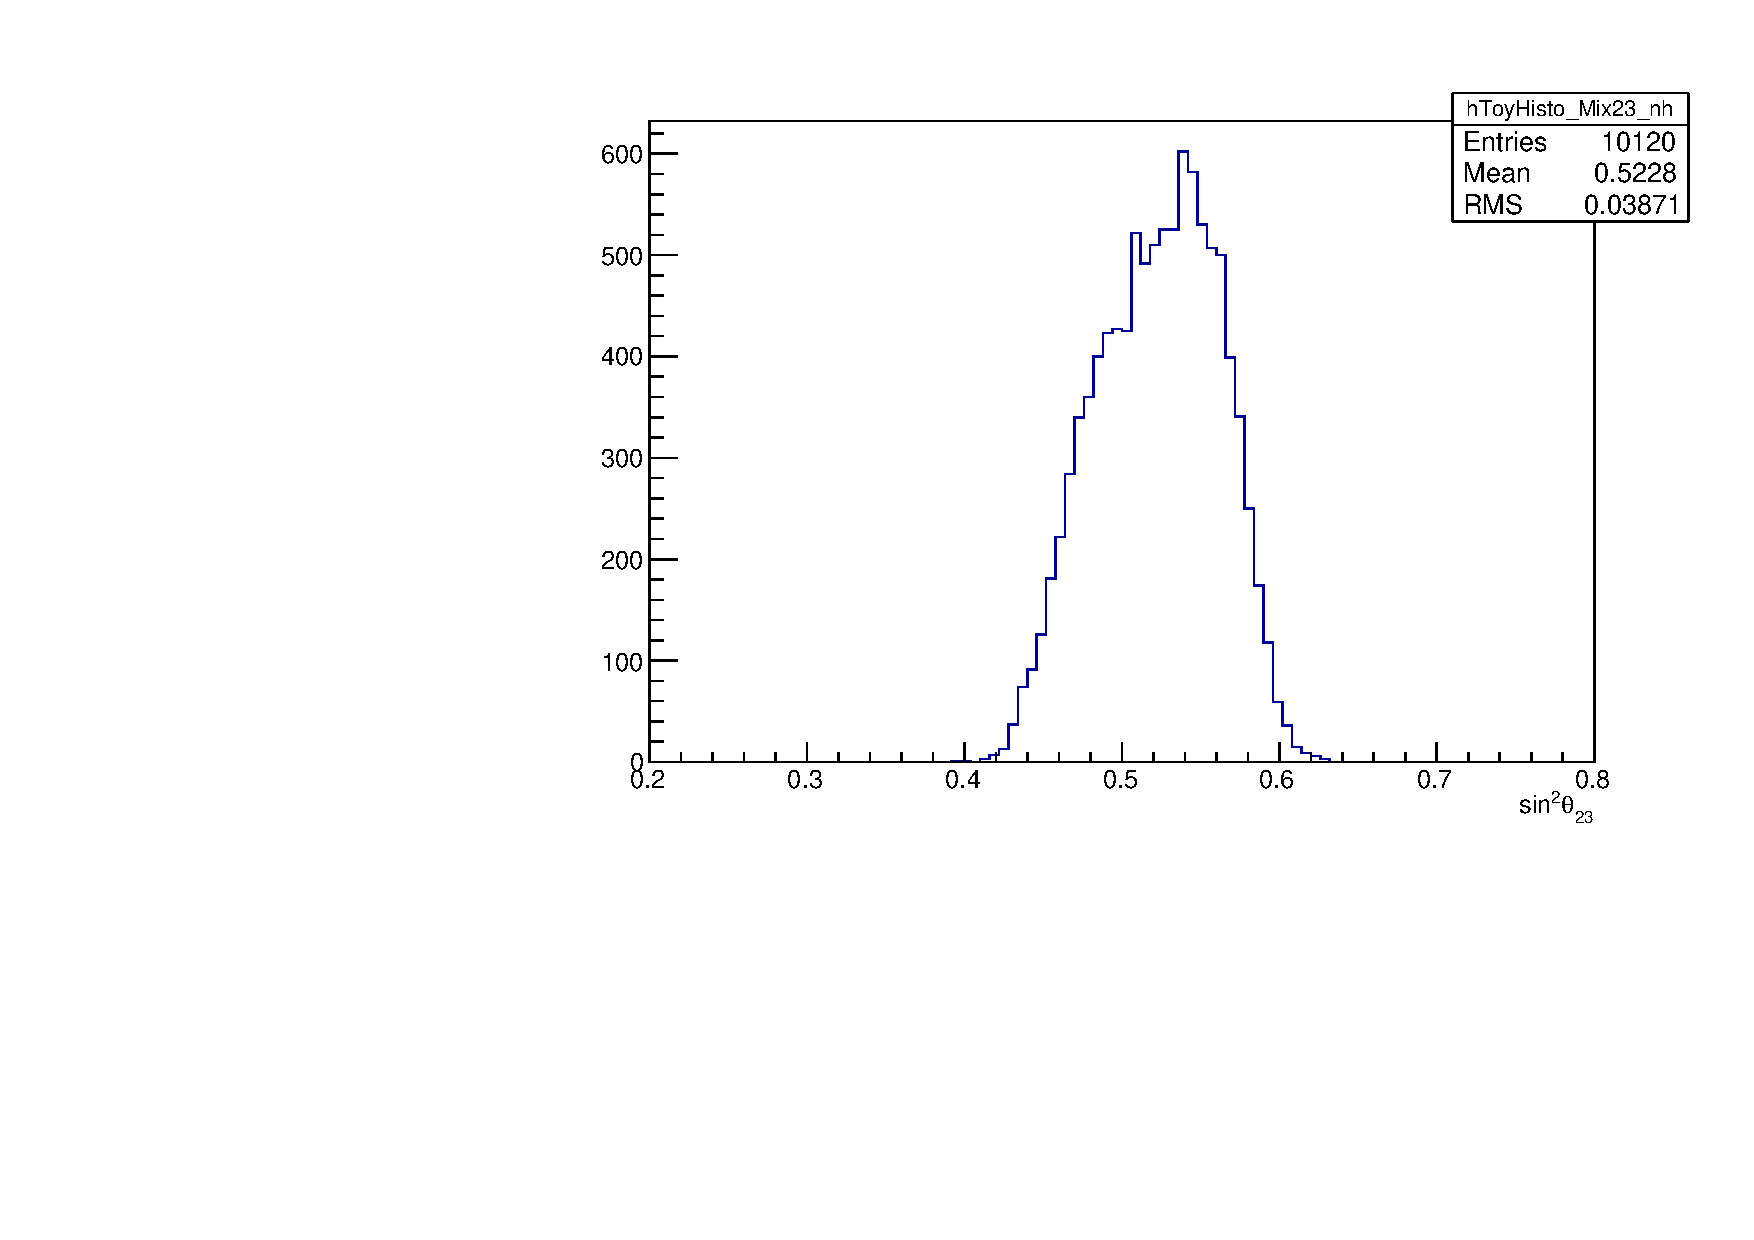
\includegraphics[width=0.9\textwidth]{data/fc/inputs/mixing23_in}
		\caption{\ssqthtwothree}
	\end{subfigure}
	\begin{subfigure}[b]{0.49\textwidth}
		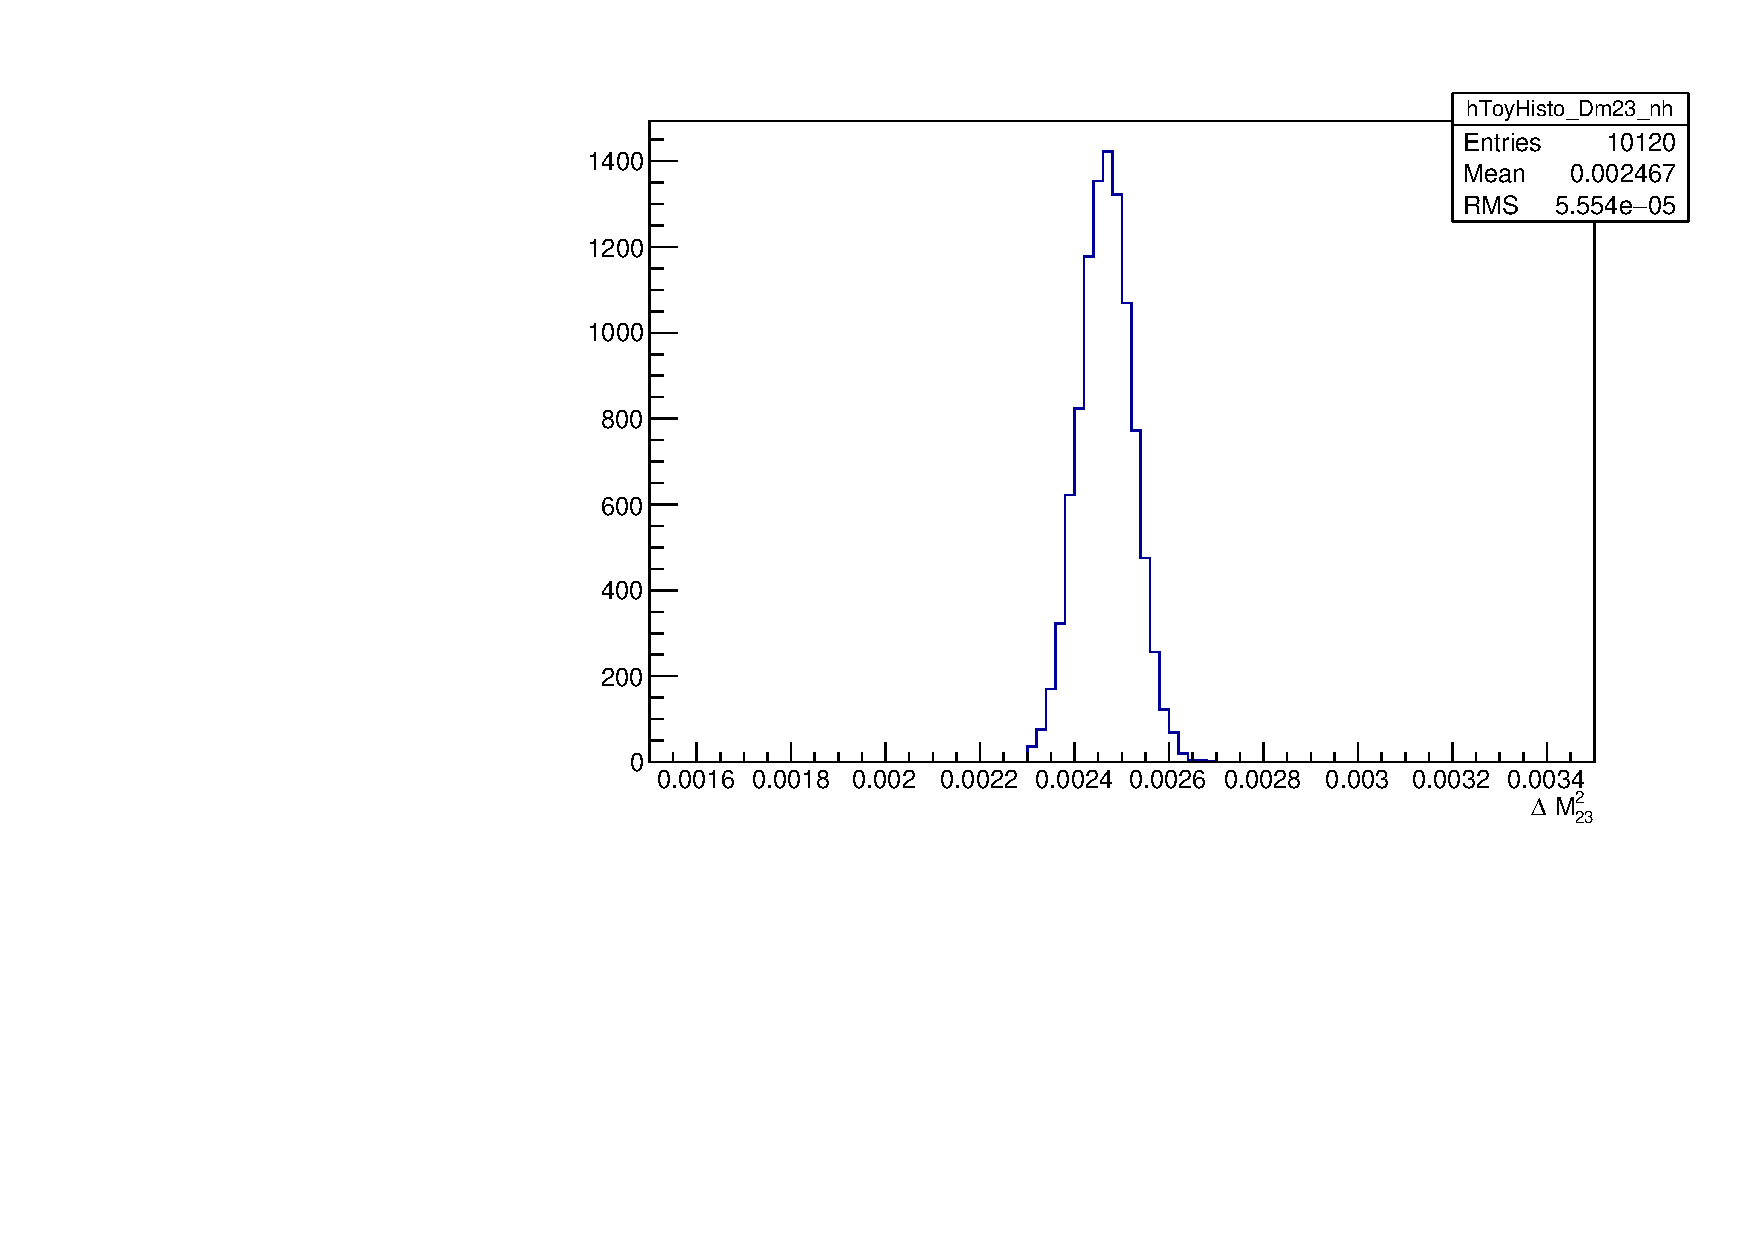
\includegraphics[width=0.9\textwidth]{data/fc/inputs/dm23_in}
		\caption{\dmsqtwothree}
	\end{subfigure}
	\begin{subfigure}[b]{0.49\textwidth}
		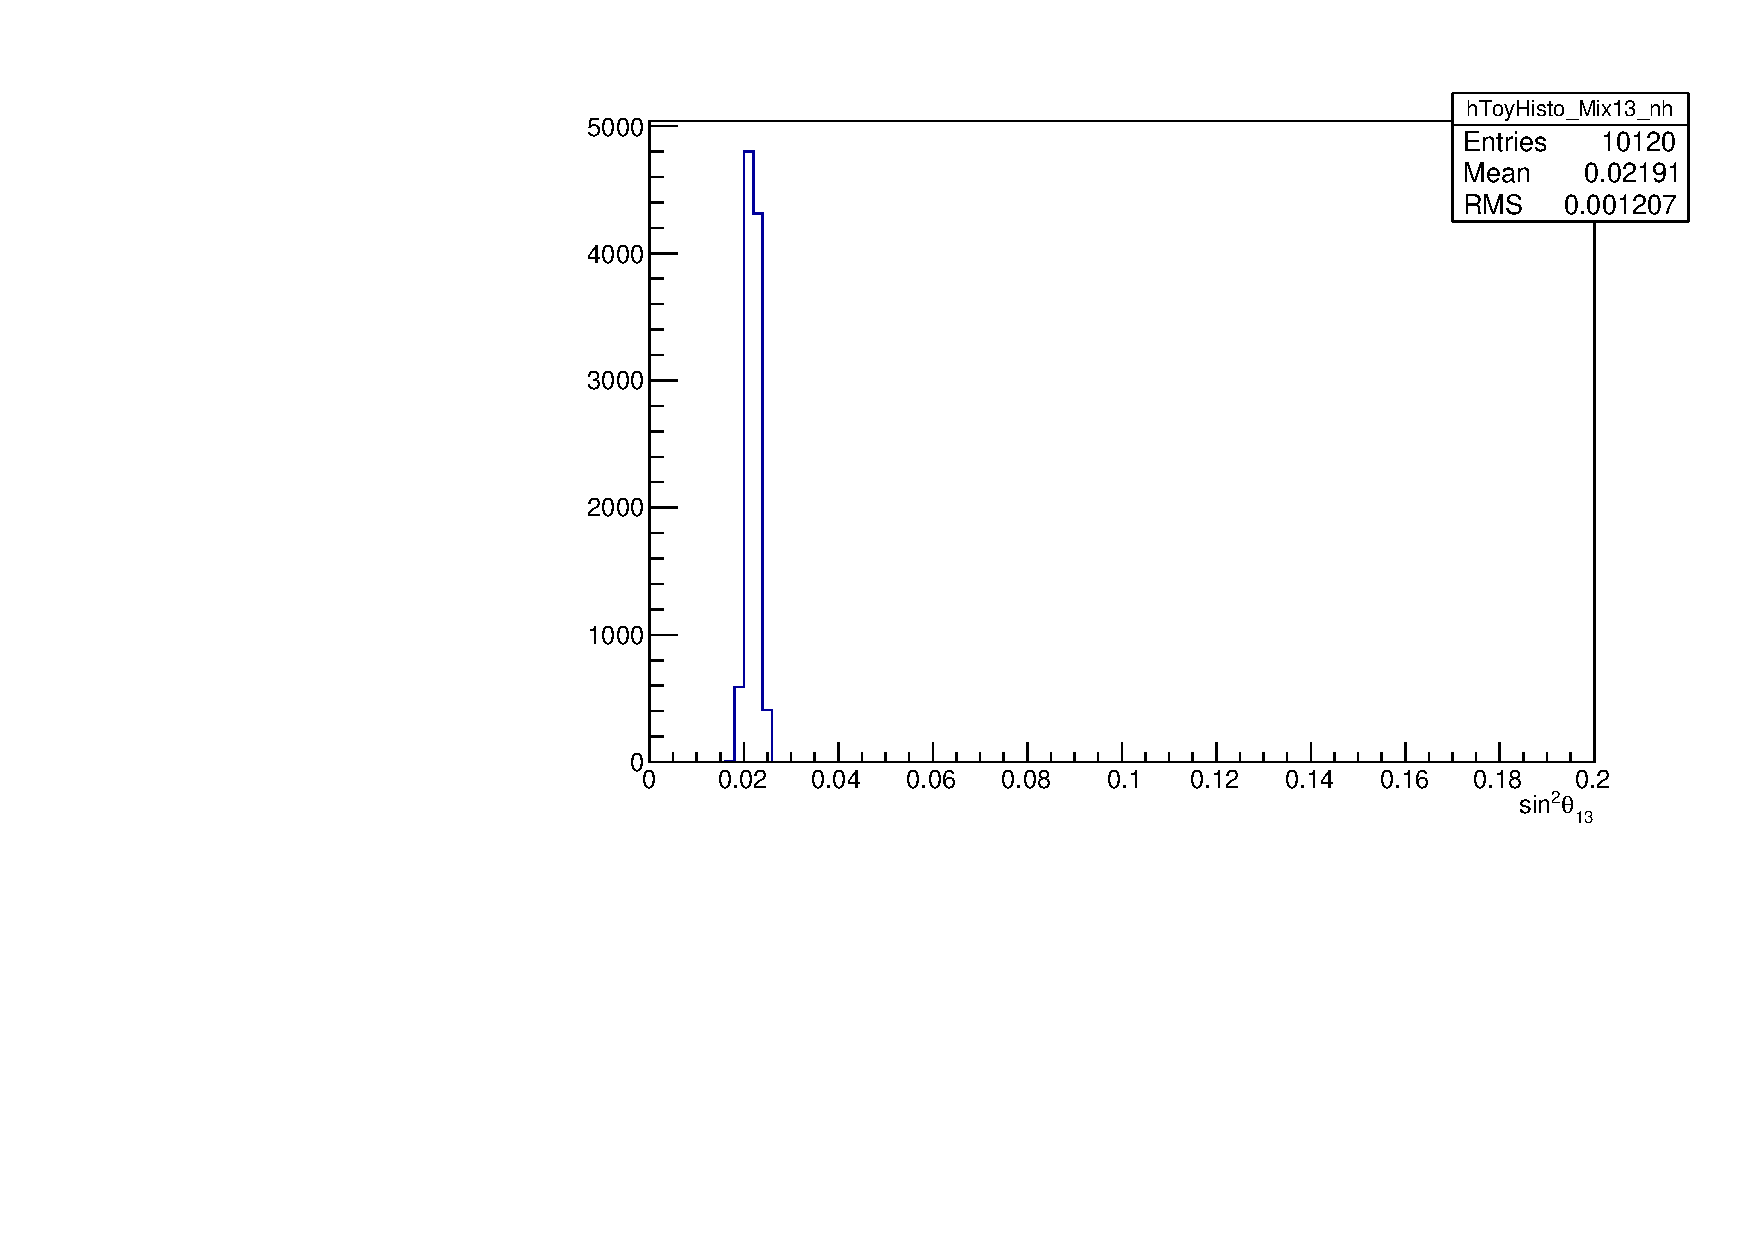
\includegraphics[width=0.9\textwidth]{data/fc/inputs/mixing13_in}
		\caption{\ssqthonethree}
	\end{subfigure}
	\caption {
		Distribution of oscillation parameter throws for Feldman-Cousins fits.
	}
	\label{fig:fc_input_dist}
\end{figure*}

\begin{figure*}[htb]
	\begin{subfigure}[b]{0.49\textwidth}
		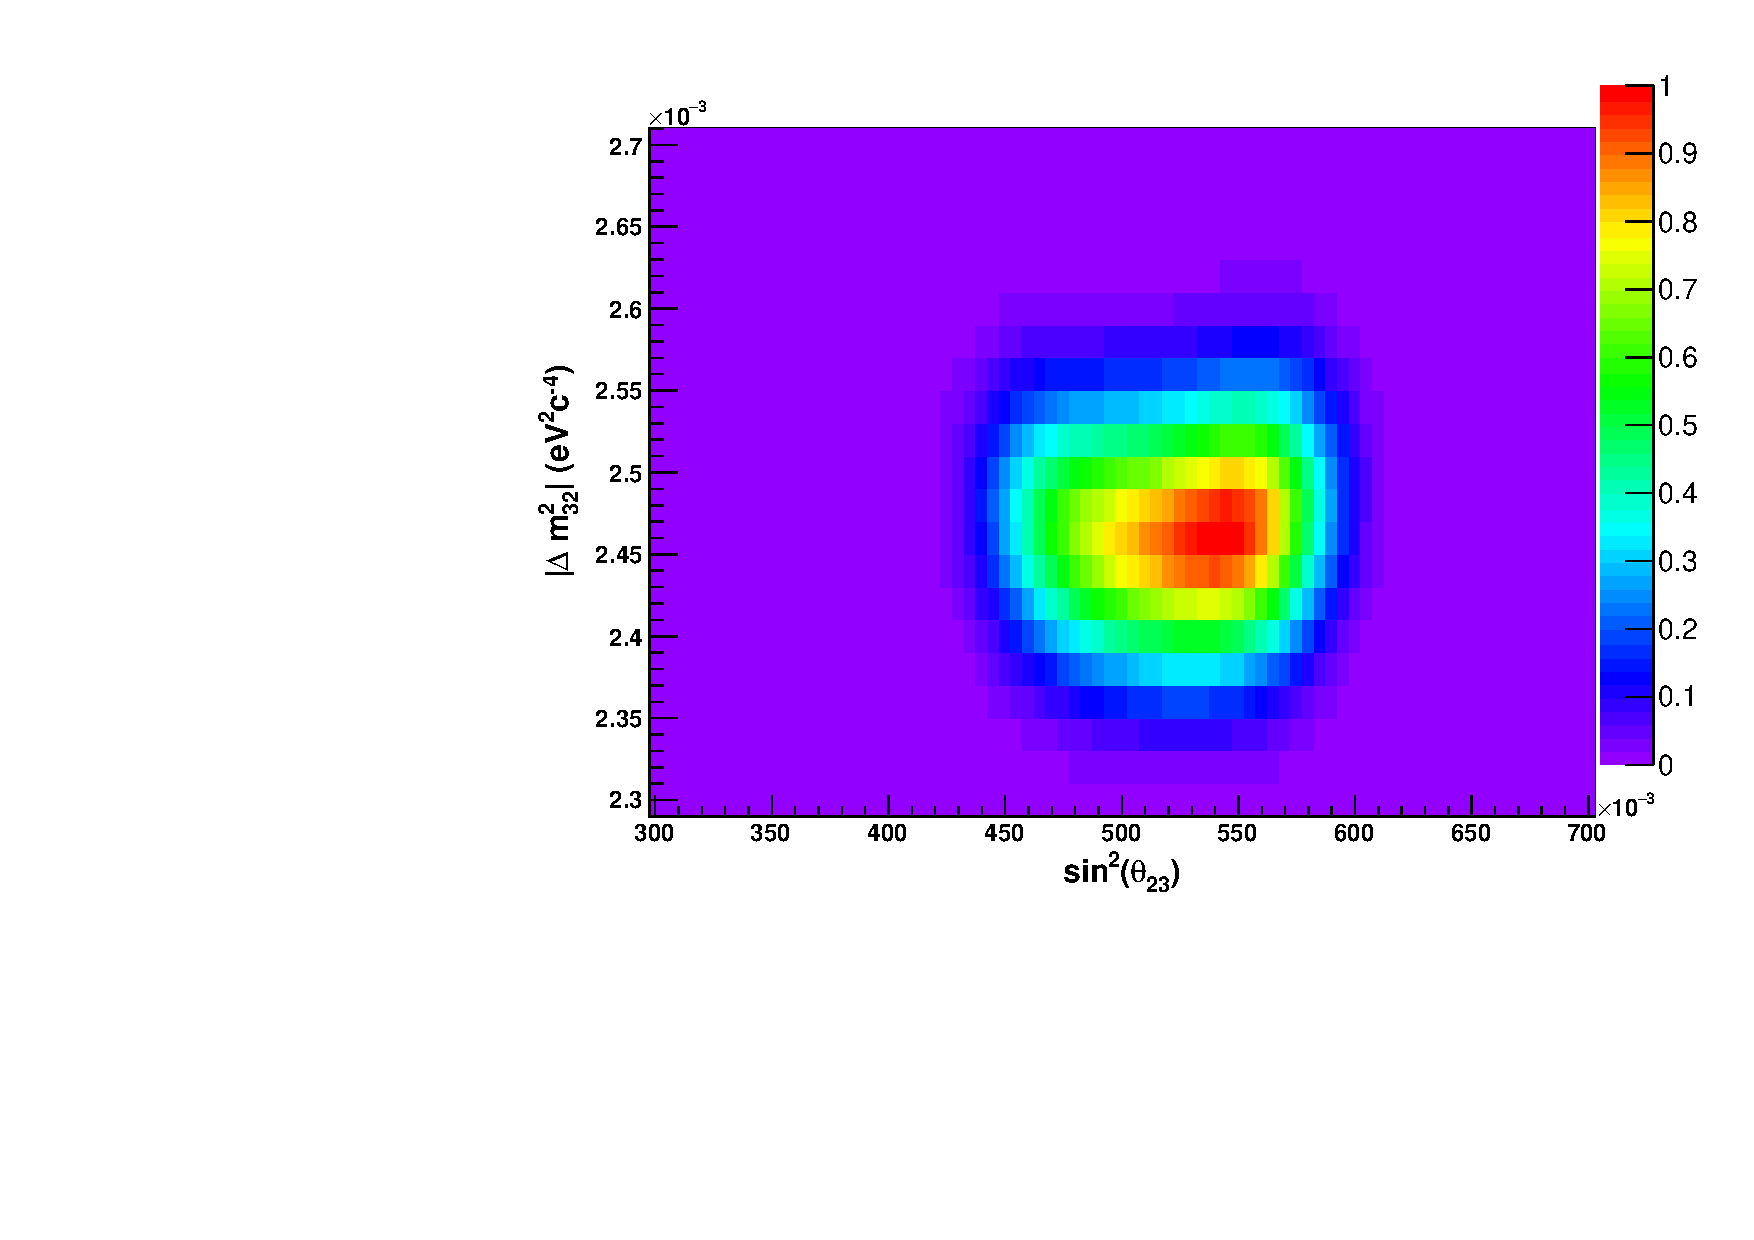
\includegraphics[width=0.9\textwidth]{data/fc/inputs/disappearance_nh_likelihood}
		\caption{Normal hierarchy}
	\end{subfigure}
	\begin{subfigure}[b]{0.49\textwidth}
		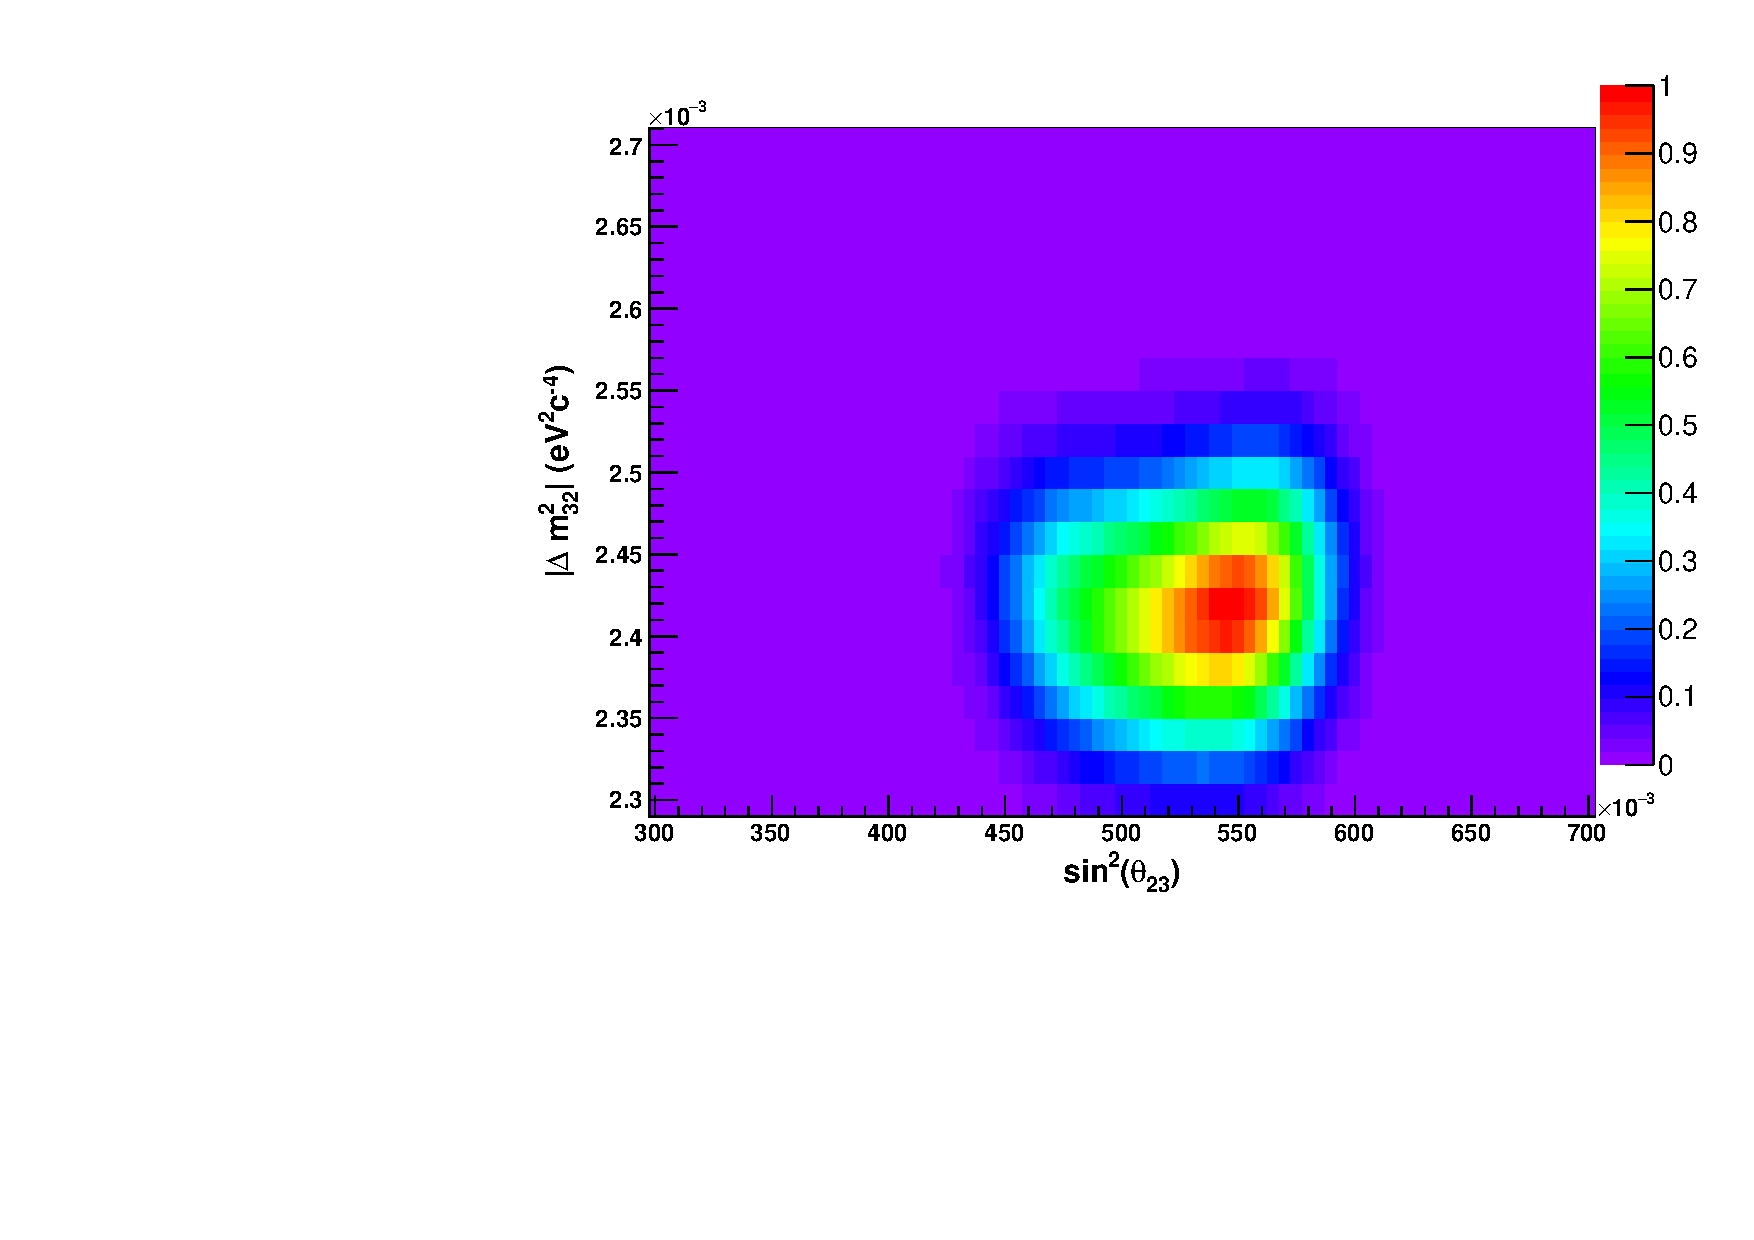
\includegraphics[width=0.9\textwidth]{data/fc/inputs/disappearance_ih_likelihood}
		\caption{Inverted hierarchy}
	\end{subfigure}
	\caption {
		Likelihood surfaces for throws of the disappearance parameter.
	}
	\label{fig:fc_input_disapp}
\end{figure*}

\subsubsection{Feldman-Cousins critical values and confidence intervals}
\label{sec:fc_significance:intervals}

In \cref{fig:fc_interval} the confidence intervals obtained with the `Feldman-Cousins' method are shown for \deltacp and mass hierarchy with reactor constraint for the \RunPeriod data set. The critical values at 90\%, $2\sigma$ and $3\sigma$ CL are computed for both the mass hierarchies at the following true values of \deltacp; $-\pi$, $-3\pi/4$, $-\pi/2$, $-\pi/4$, 0, $+\pi/4$, $+\pi/2$, $+3\pi/4$, and $+\pi$. Inverted hierarchy is almost excluded at $2\sigma$, except for a small interval around $\delta_{CP} = -\pi/2$. Both $\delta_{CP} = 0$ and $\delta_{CP} = \pi$ are excluded at $2\sigma$. In \cref{tab:fc_interval} the $2\sigma$ CL intervals for \deltacp versus mass hierarchy, obtained with the Feldman-Cousins method, are shown.

\begin{figure*}[htb]
	\center
	\begin{subfigure}[b]{0.6\textwidth}
		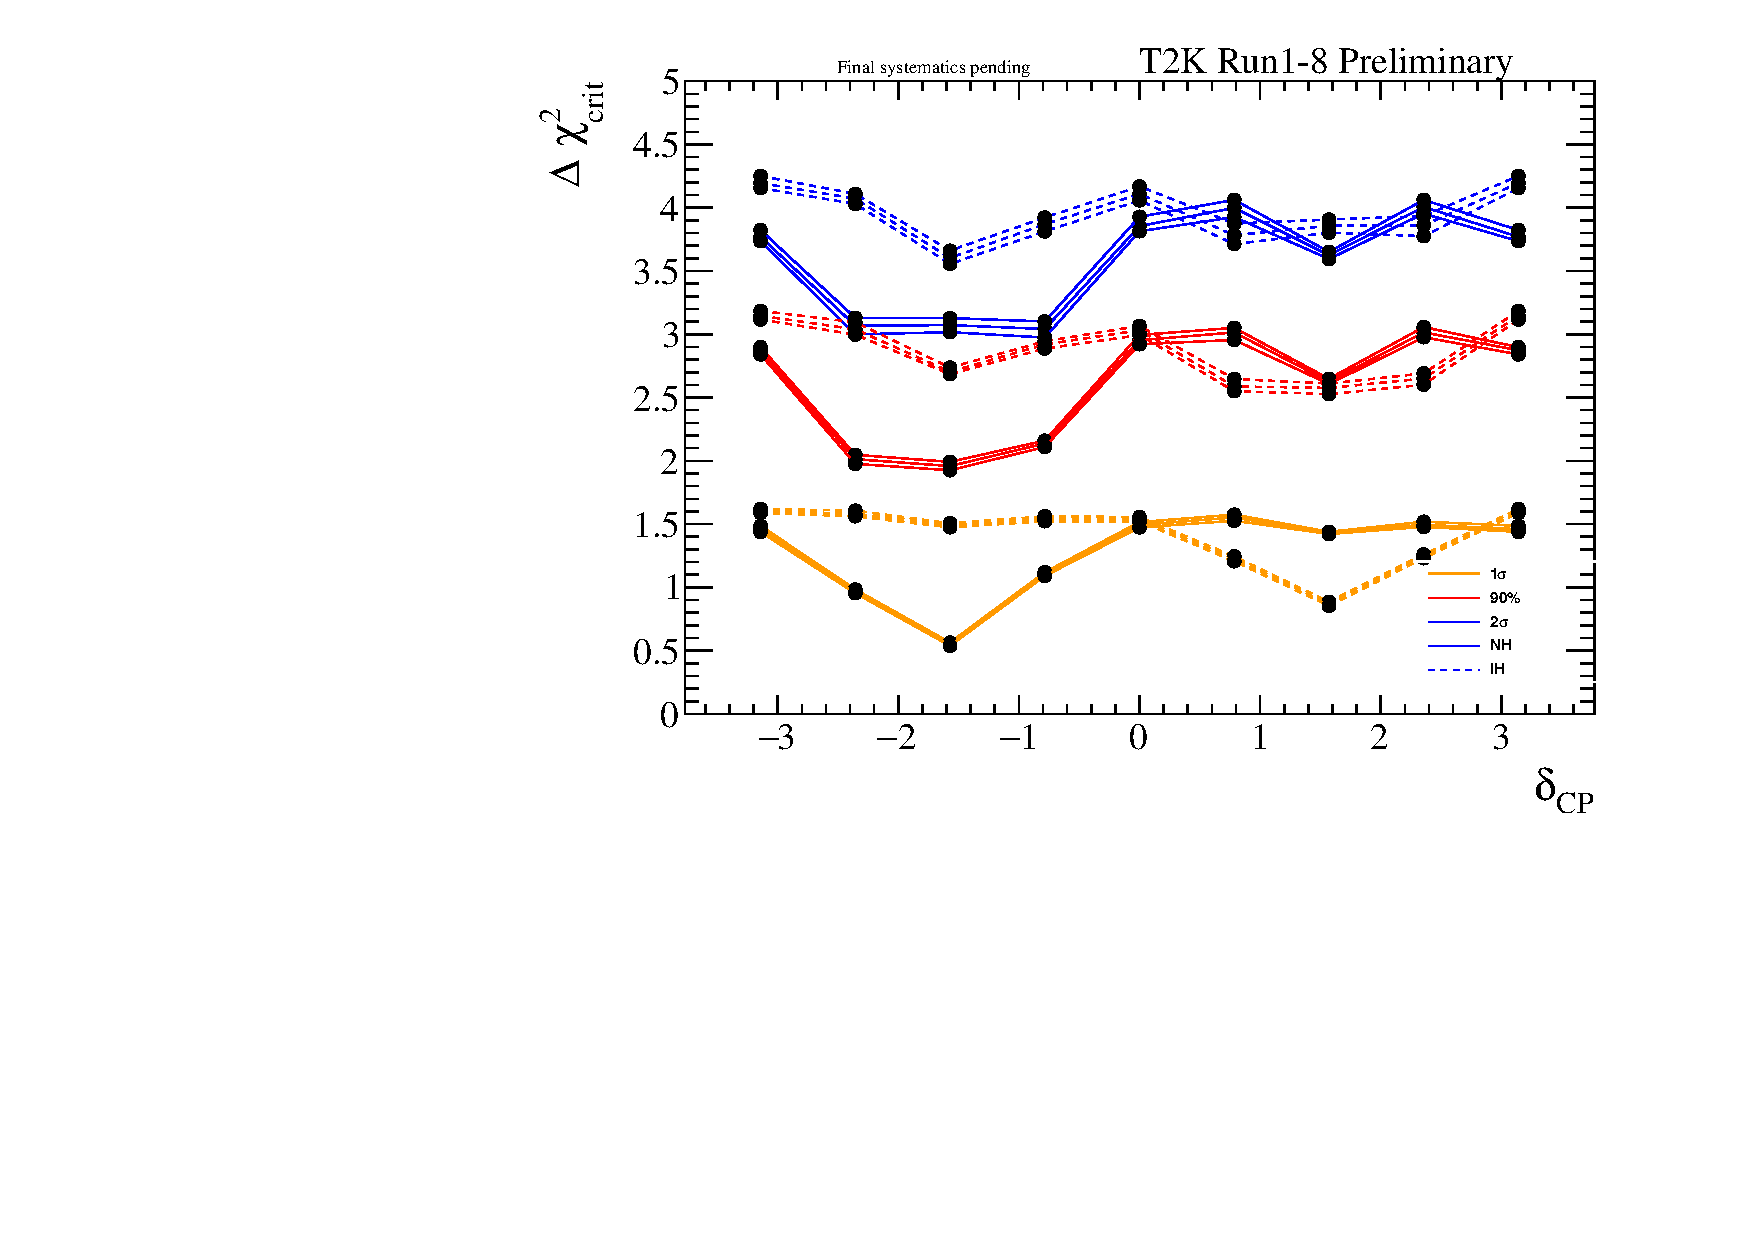
\includegraphics[width=0.9\textwidth]{data/fc/FC_critical_values}
		\caption{\label{fig:fc_critval}Critical $\Delta\chi^2$ values}
	\end{subfigure}
	\begin{subfigure}[b]{0.49\textwidth}
		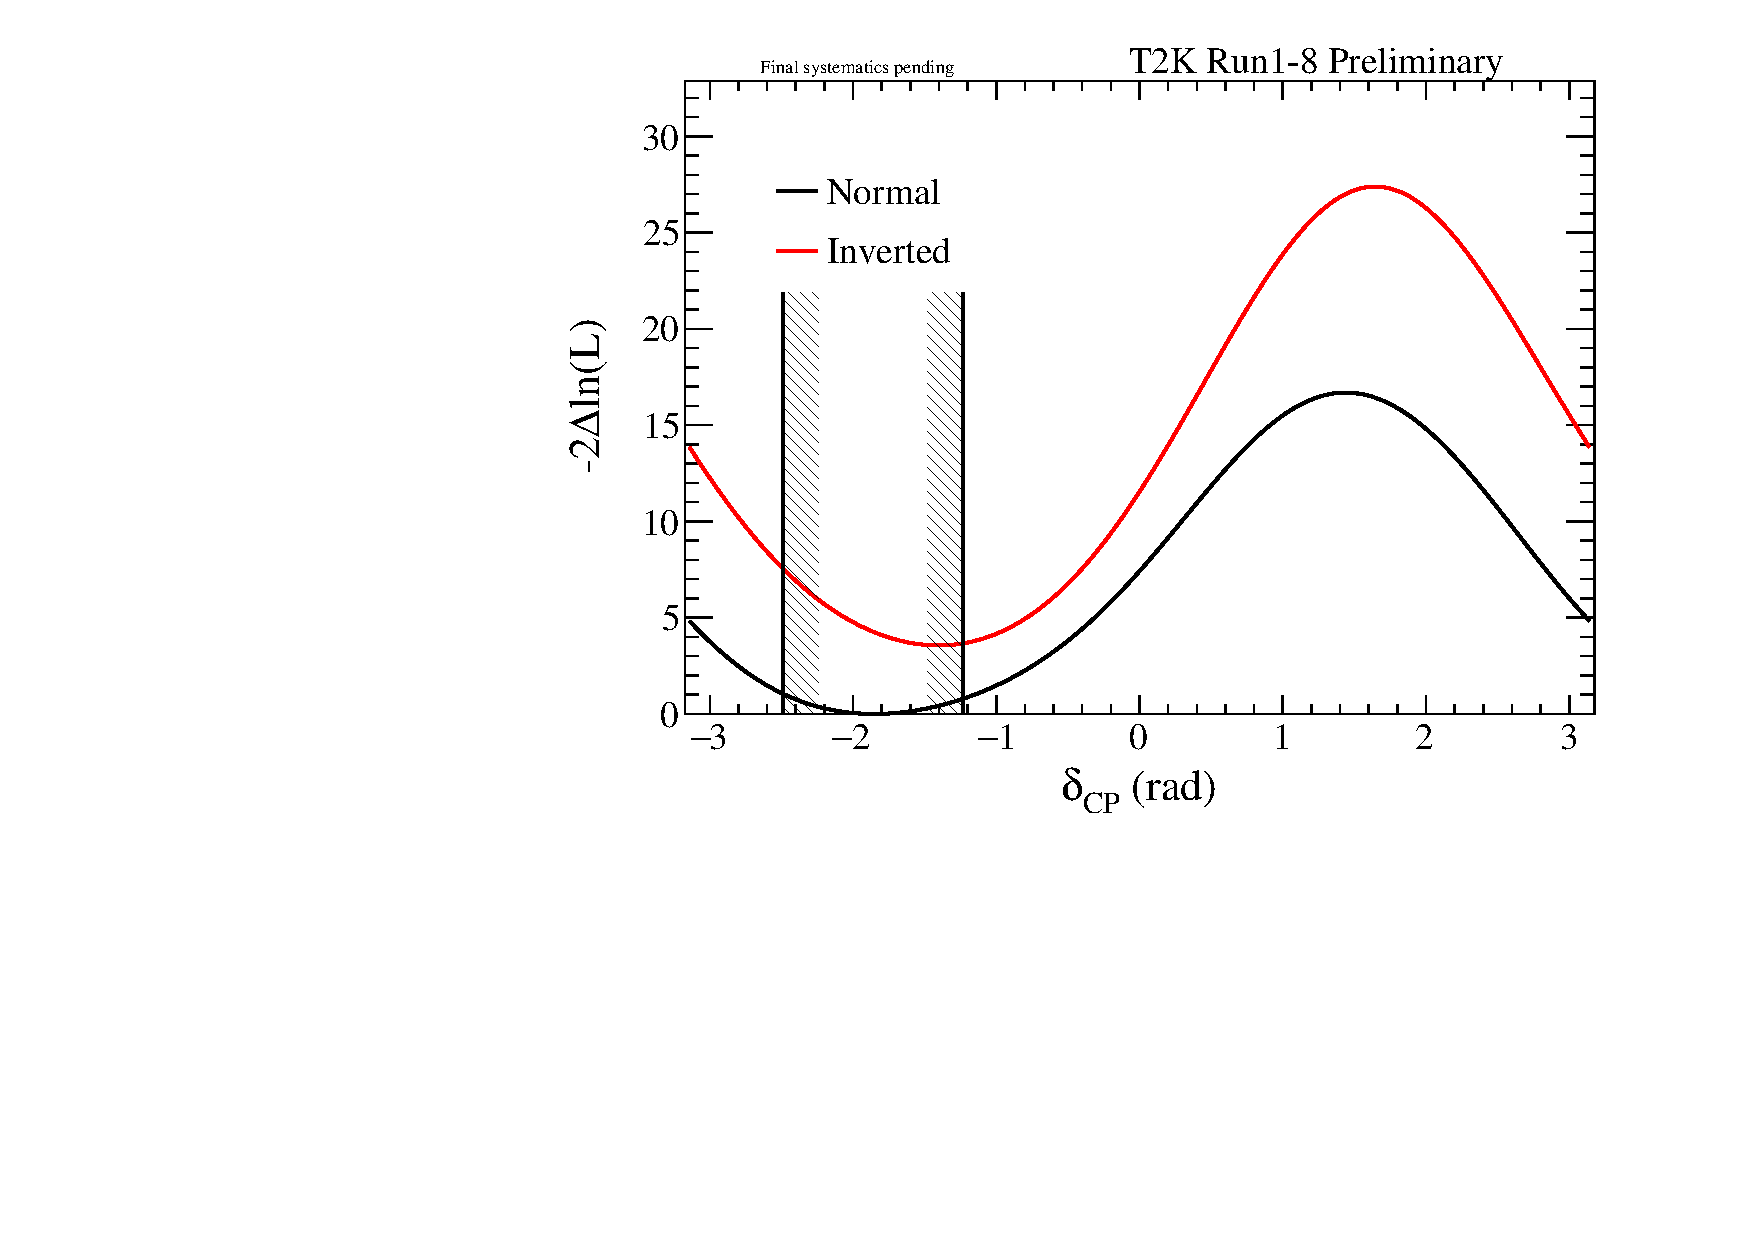
\includegraphics[width=0.9\textwidth]{data/fc/dcp_FC_1sigma_CL}
		\caption{$1\sigma$ CL exclusion region}
	\end{subfigure}
	\begin{subfigure}[b]{0.49\textwidth}
		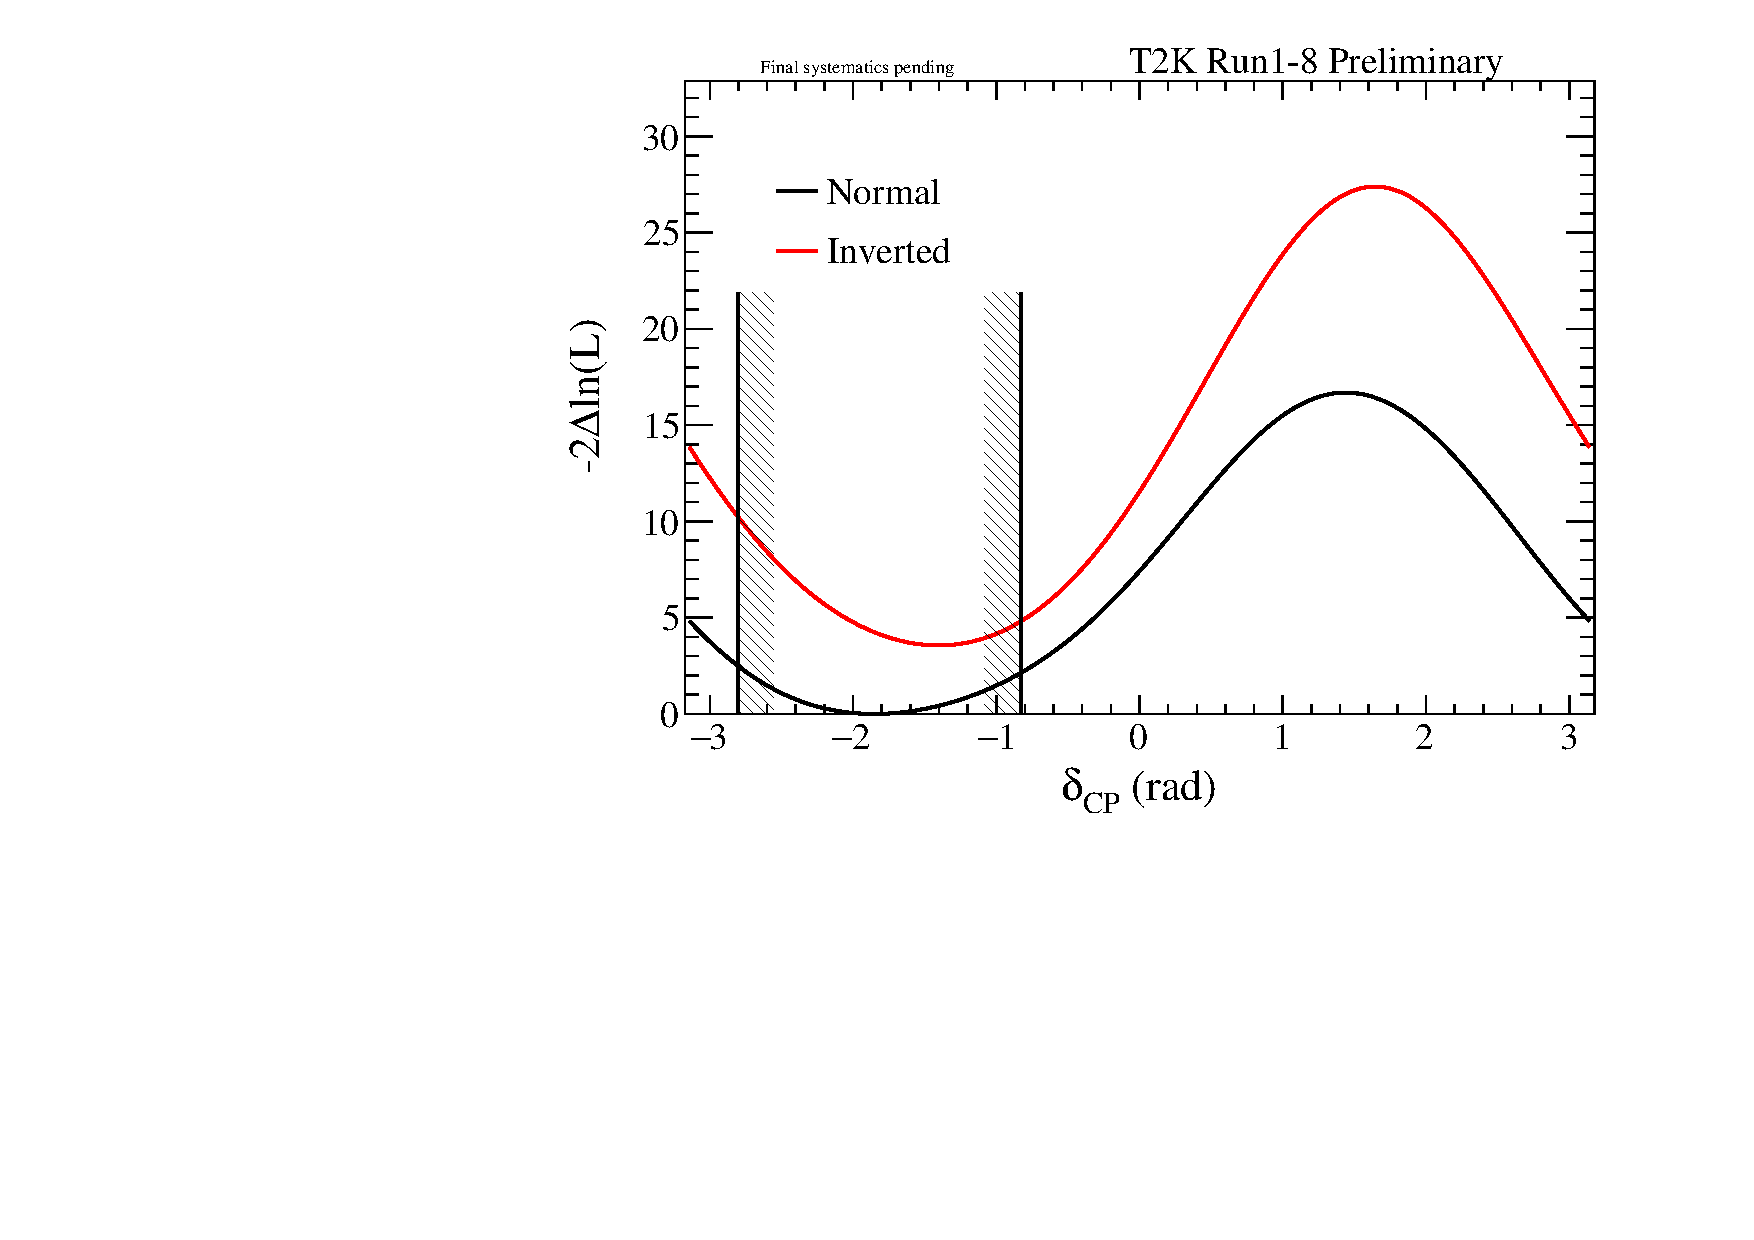
\includegraphics[width=0.9\textwidth]{data/fc/dcp_FC_90_CL}
		\caption{90\% CL exclusion region}
	\end{subfigure}
	\begin{subfigure}[b]{0.49\textwidth}
		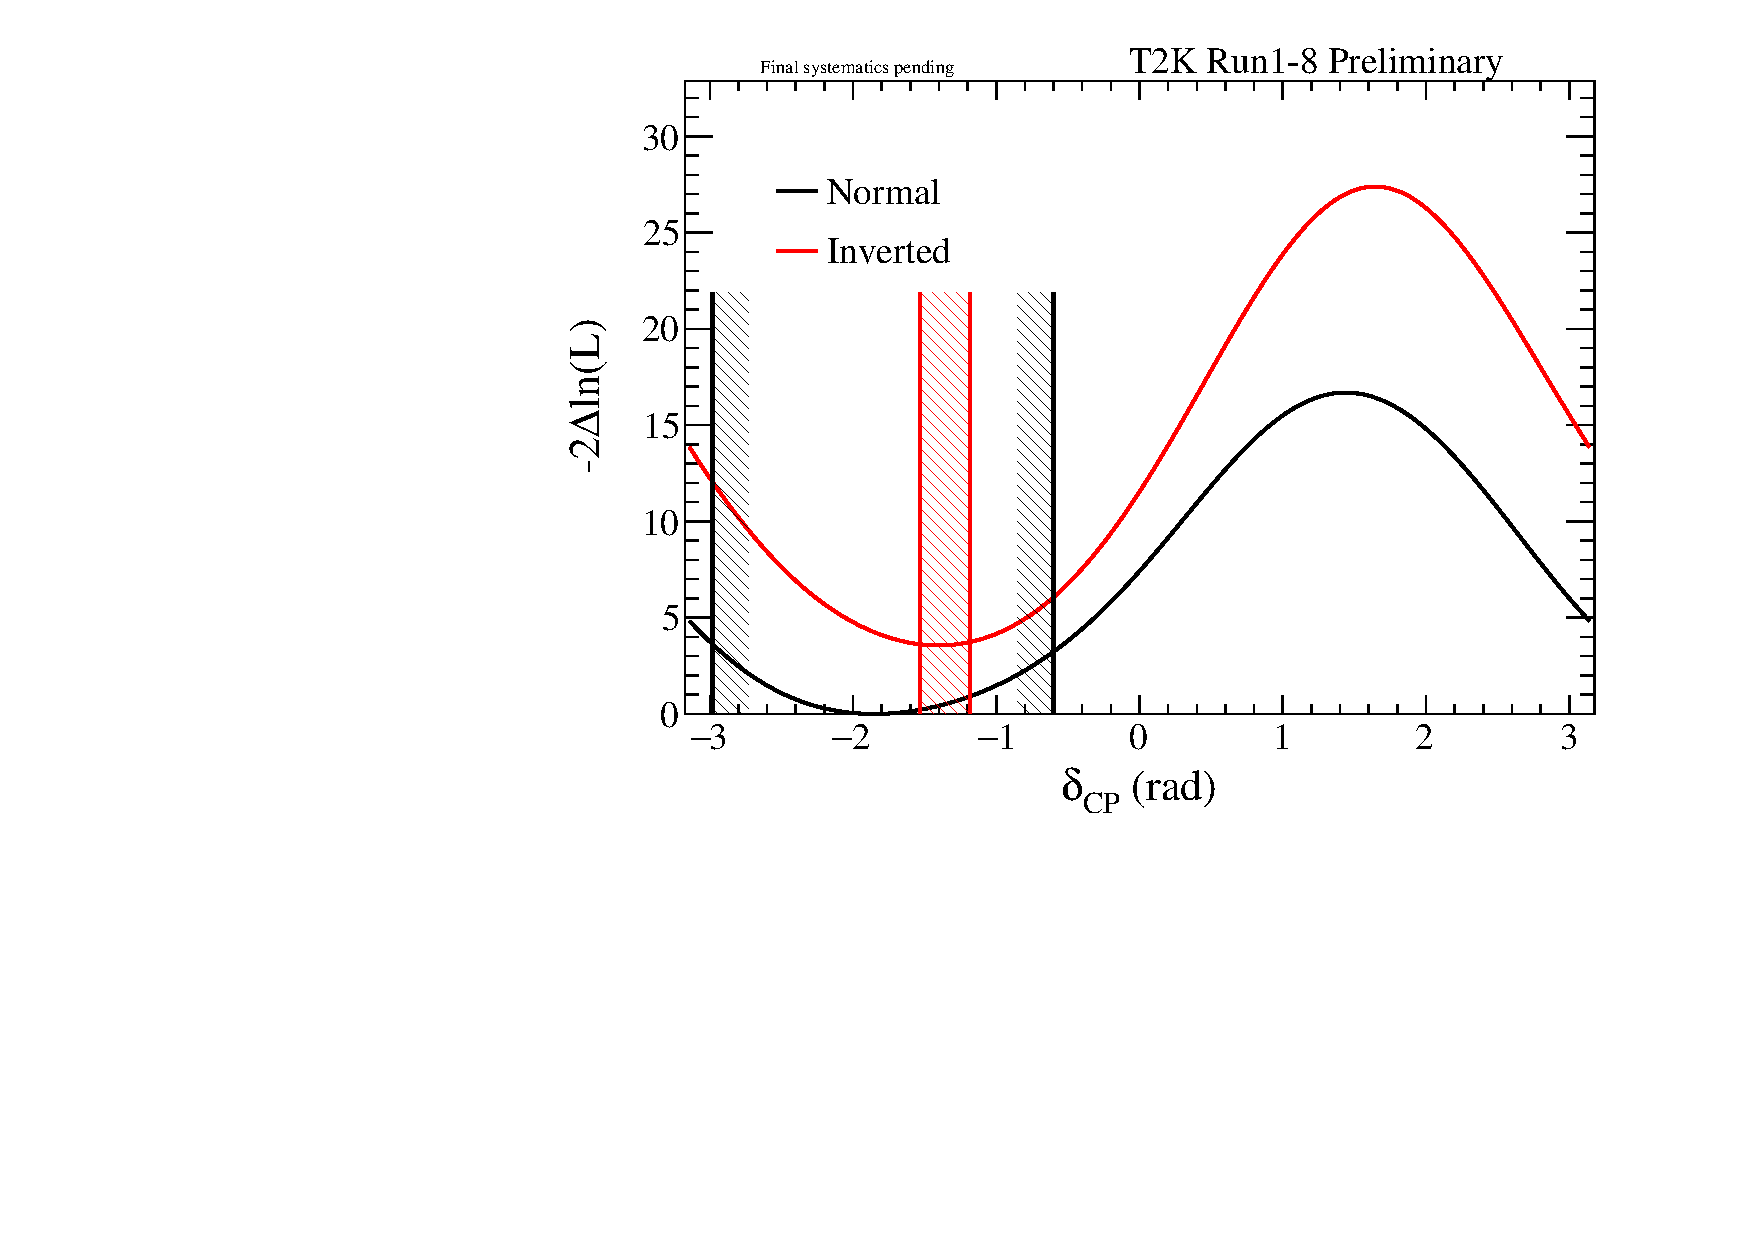
\includegraphics[width=0.9\textwidth]{data/fc/dcp_FC_2sigma_CL}
		\caption{$2\sigma$ CL exclusion region}
	\end{subfigure}
	\caption {
$\Delta\chi^2$ critical values and confidence intervals for the measured $\Delta\chi^2$ distributions for \RunPeriod. Critical values obtained with the Feldman-Cousins method for \RunPeriod for 9 evenly spaced values on the range \( \left[-\pi,\pi\right] \). Critical values are shown for 1\( \sigma \), 2\( \sigma \) and 90\% CL for normal (solid lines) and inverted (dashed lines) hierarchies. At least \num{1e4} toy experiments are performed for each point. The three bands of lines show the \( \pm 1\sigma \) uncertainty on the critical values. Also shown are the measured \( \Delta \chi^2 \) distributions shifted with respect to the same global minium and the $1\sigma$, 90\% and $2\sigma$ exclusion regions for both mass hierarchies. 
	}
	\label{fig:fc_interval}
\end{figure*}

\begin{table}[htb]
	\centering
	\begin{tabular}{| c | c | c | c | c |}
\hline
Parameter & Reactor & CL & Normal hierarchy & Inverted hierarchy \\
\hline
\deltacp		& Yes & 90\% & $\left[ -2.805, -0.830 \right]$ & - \\
\deltacp		& Yes & $ 2\sigma $ & $\left[ -2.981, -0.600 \right]$ & $\left[ -1.531, -1.184 \right]$ \\
\hline
\end{tabular}

	\caption{
		The confidence intervals at 90\% CL and $2\sigma$ CL obtained with the Feldman-Cousins method for the \RunPeriod data set is shown for the measurement of \deltacp versus mass hierarchy.
	}
	\label{tab:fc_interval}
\end{table}

%
%
%In \cref{fig:joint_dcp_fc_run17c} the confidence intervals obtained with the ``Feldman-Cousins" method
%are shown for $\delta_{CP}$ and mass hierarchy with reactor constraint for the Run 1-7c data set.
%The critical values at both 90\% and $2\sigma$ CL are computed
%for both the mass hierarchies and the following true values of $\delta_{CP}$: 
%$-\pi$, -2.356, $-\pi/2$, -0.785, 0, +0.785, $+\pi/2$, -2.356, $+\pi$. 
%The procedure described in \cref{sec:cl} is used.
%About 10k toy experiments were used for all the true points except $\delta_{CP} = \pi$ - normal hierarchy.
%Indeed the Run 1-7c data $\Delta \chi^2$ value is very close to the 90\% CL critical value, within one standard deviation of the critical value,
%if only 10k toy experiments are used. 
%For this reason, in order to provide a more precise statement about the 
%90\% CL exclusion of $\delta_{CP} = \pi$ - normal hierarchy, about 28k toy experiments are used, 
%so that the data $\Delta \chi^2$ value is outside the $\pm 1 \sigma$ critical value error.
%This can be seen in in \cref{fig:joint_dcp_fc_run17c}
%where the $\pm 1 \sigma$ error on the critical values are shown as well.
%The same procedure used for the Run 1-6 and Run 1-7b data fit, shown in \cref{sec:fc_significance}, is used.
%Inverted hierarchy is almost excluded at 90\% CL except for a small interval around $\delta_{CP} = -\pi / 2$.
%$\delta_{CP} = 0$ is still disfavored with respect to $\delta_{CP} = \pi$, which, however, is excluded at 90\% CL. 
%We can say that CP conservation assuming the PMNS framework is excluded at 90\% CL also for the Run 1-7c data set,
%though the p-value for $\delta_{CP} = \pi$ and normal hierarchy is very close to 0.1. 
%
%\begin{figure*}[htb]
%\center
%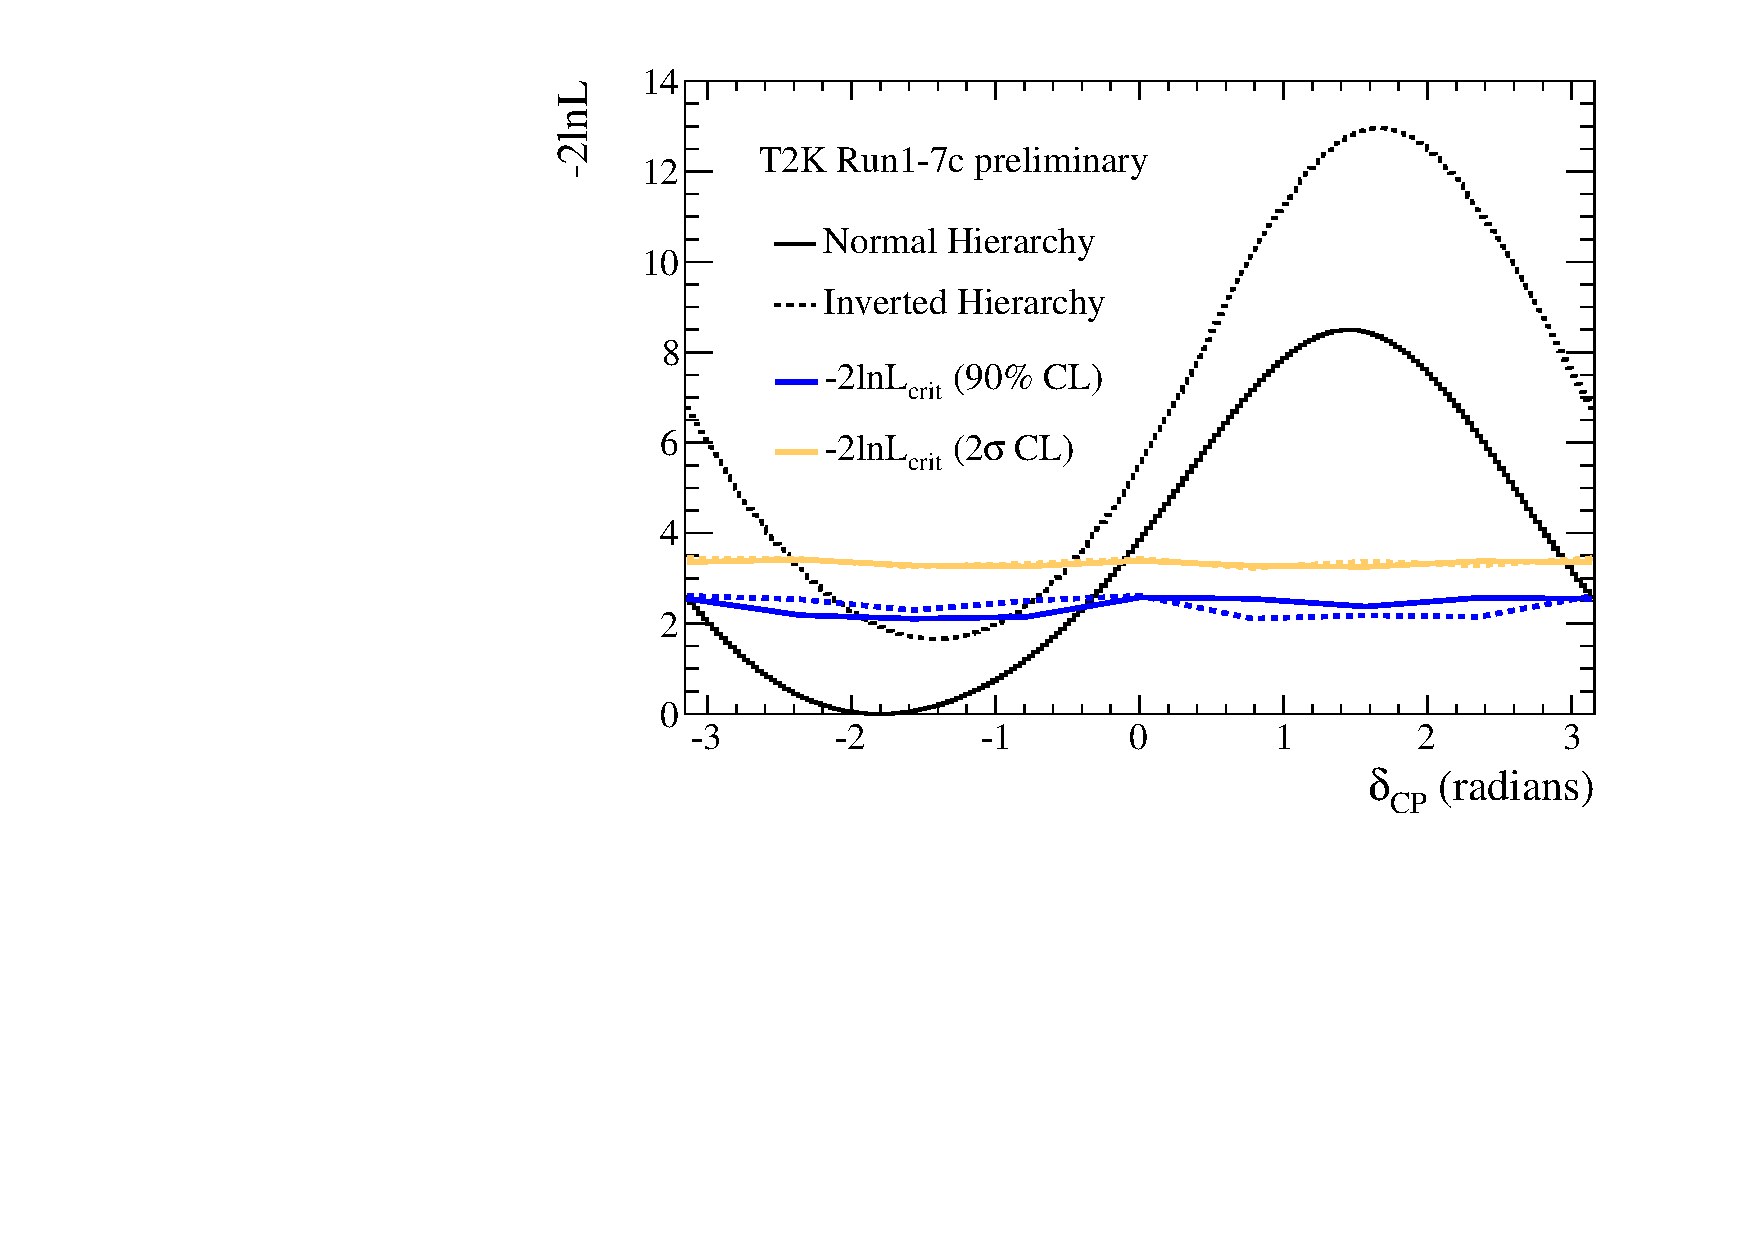
\includegraphics[width=0.49\textwidth]{joint_plots/coverage_fc/fc_run17c/dcp_mh_react_run17.pdf} 
%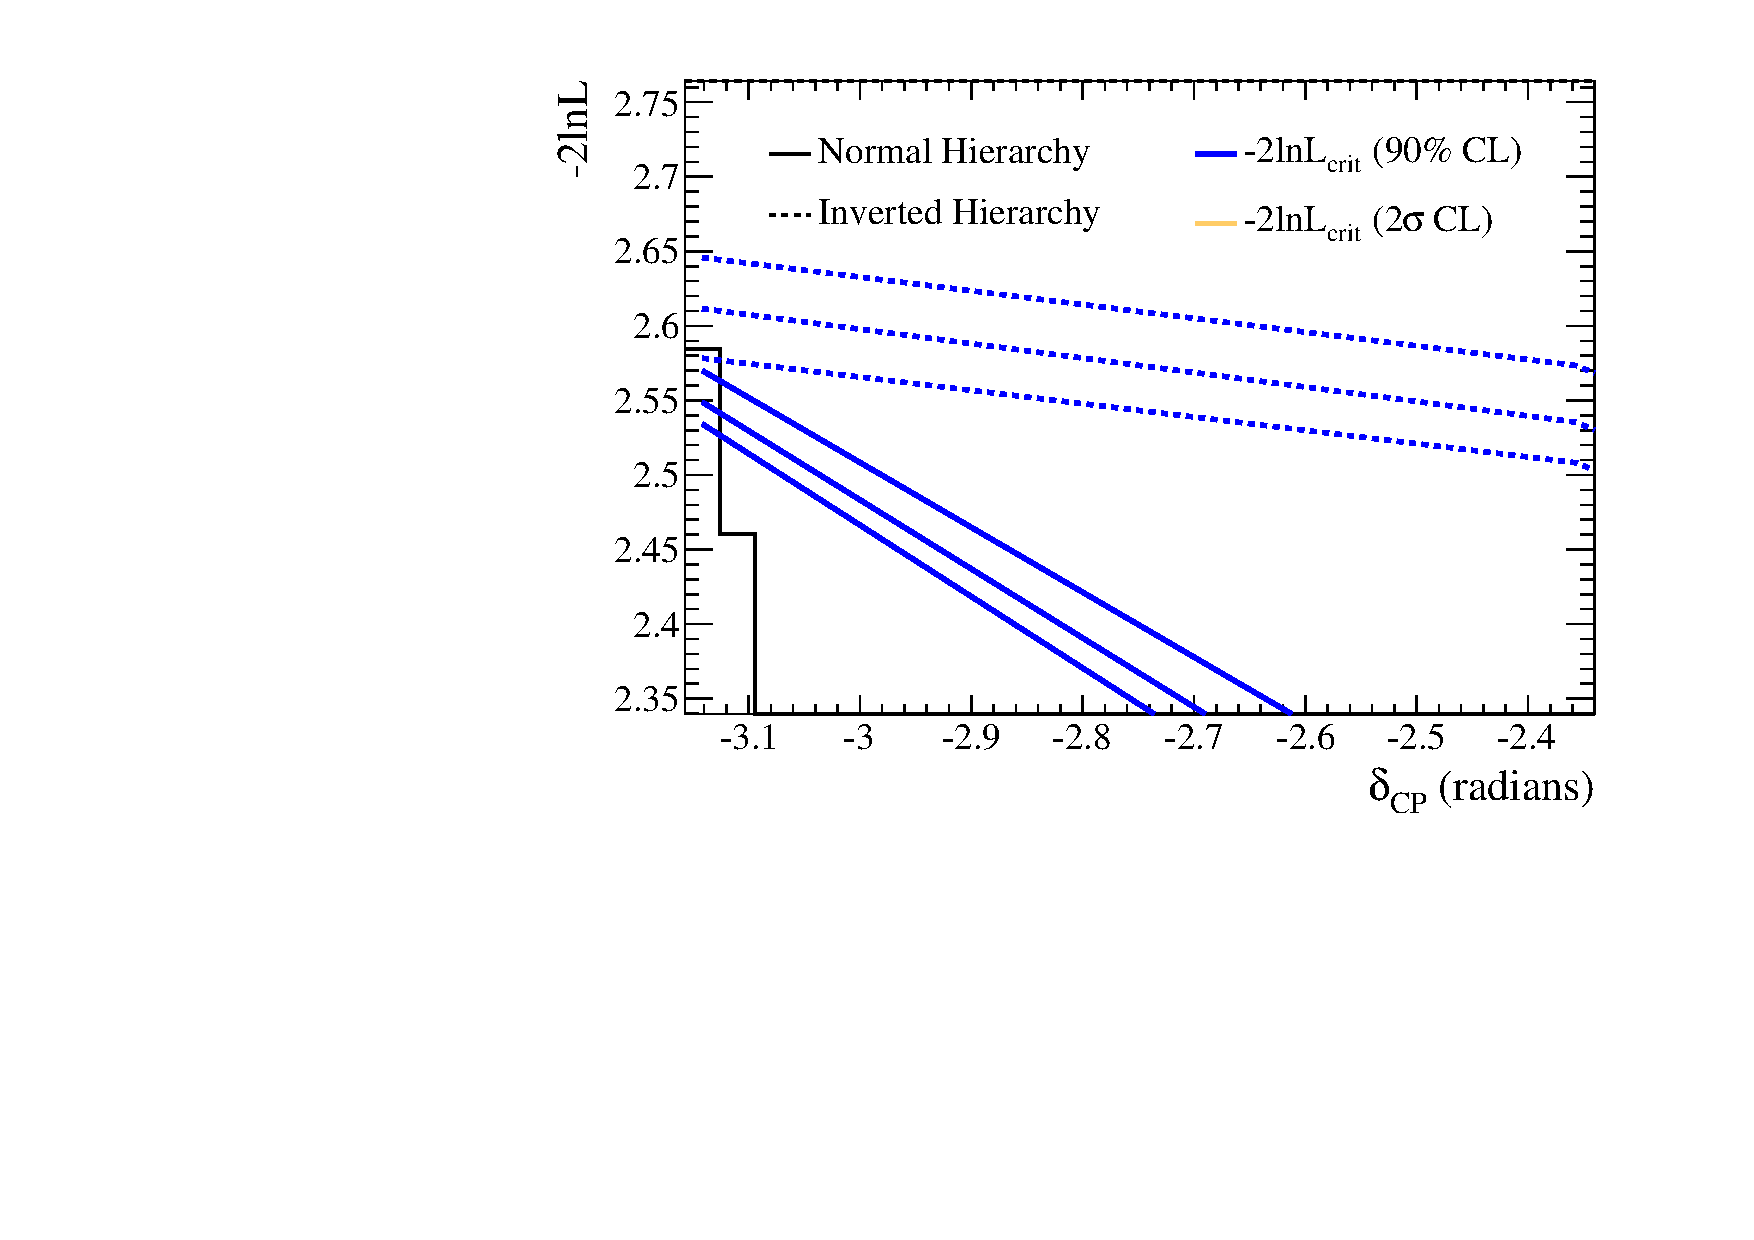
\includegraphics[width=0.49\textwidth]{joint_plots/coverage_fc/fc_run17c/dcp_mh_react_run17_zoom.pdf} \\
%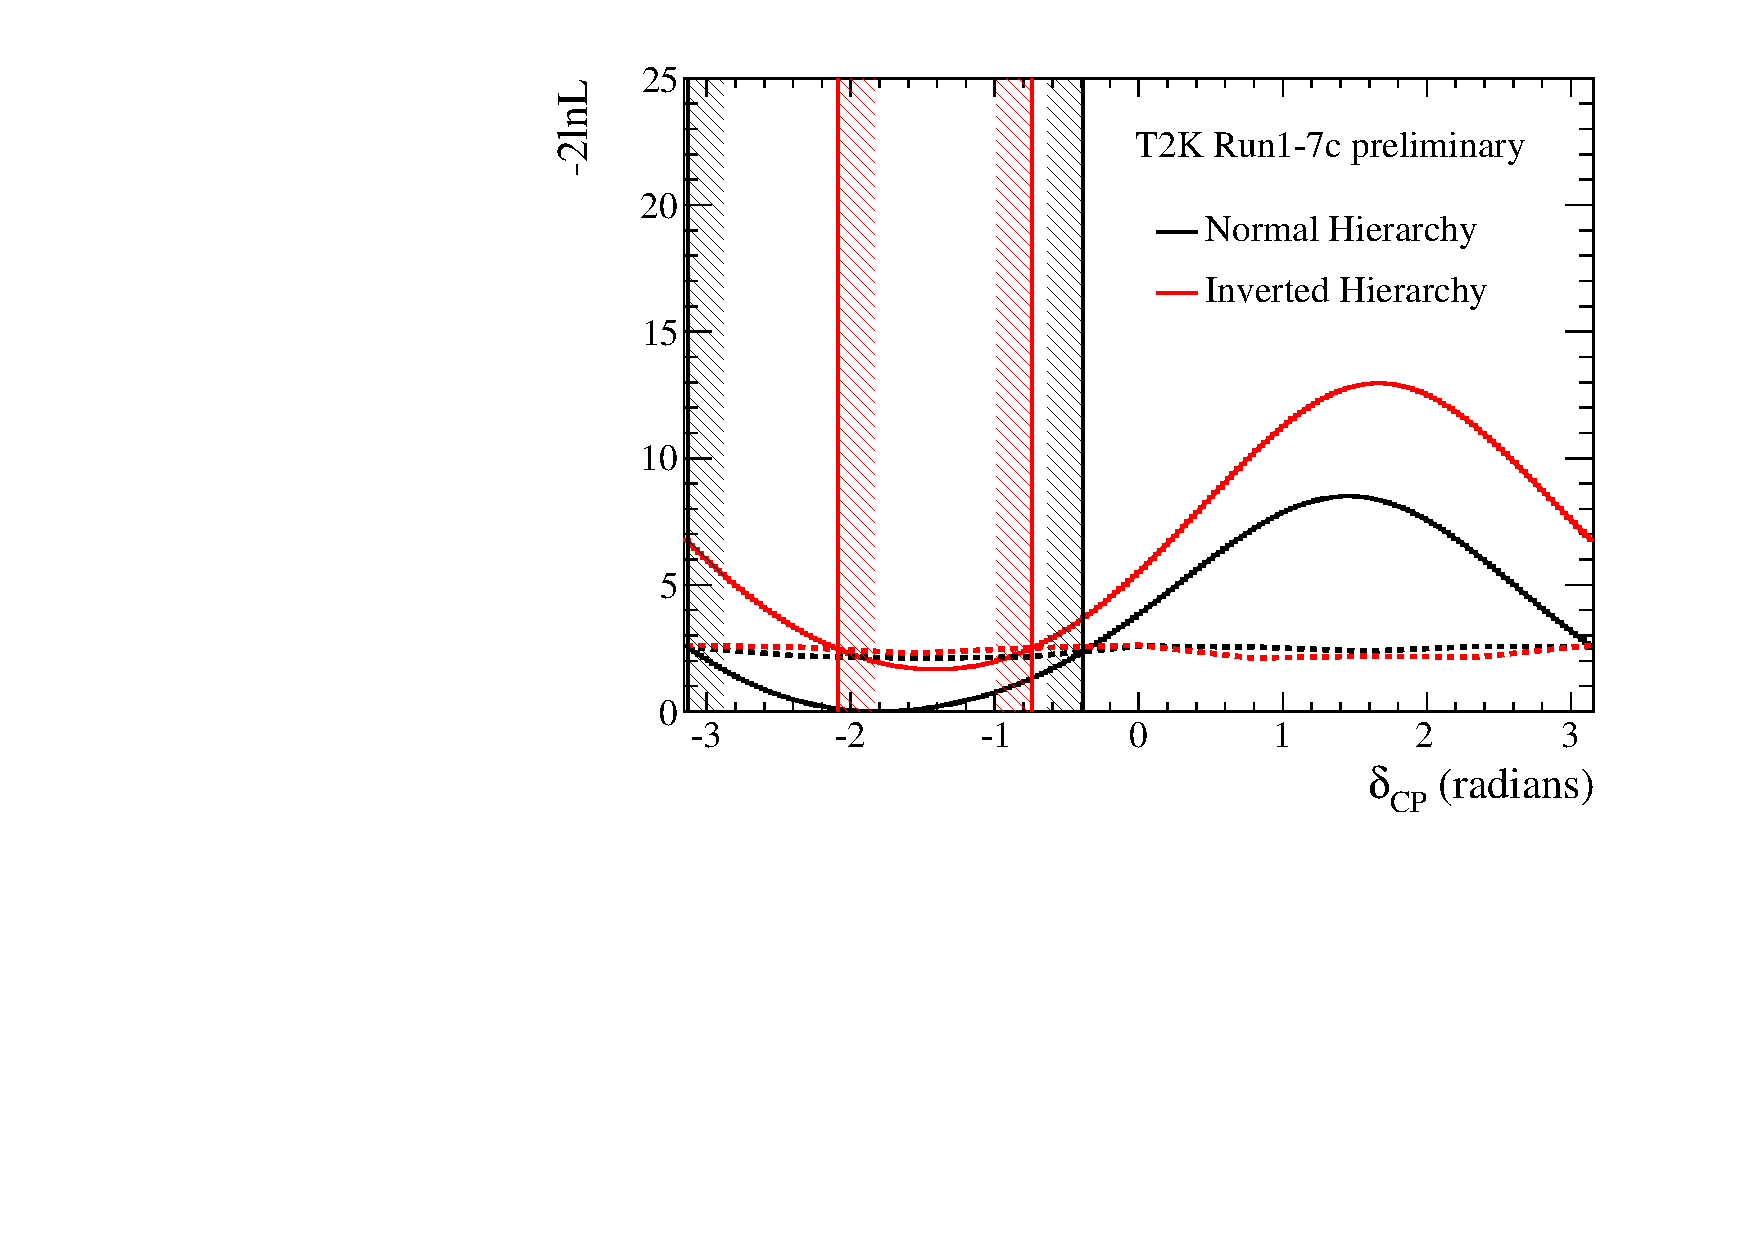
\includegraphics[width=0.49\textwidth]{joint_plots/coverage_fc/fc_run17c/dcp_mh_react_run17_interval_90CL.pdf} 
%\caption{
%Measured $\Delta \chi^2$ distributions with the full Run 1-7c data set.
%Both normal (black solid line) and inverted (black dashed line) hierarchies are shown. 
%The ``Feldman-Cousins" method is used to set the $\Delta \chi^2$ critical values in order to provide 
%confidence intervals with the proper coverage.
%The ranges of $\delta_{CP}$ which correspond to $\Delta \chi^2$ values larger than the critical 
%values (blue for 90\% CL and orange for $2\sigma$ CL) are excluded at a certain confidence level.
%Both normal and inverted hierarchy $\Delta \chi^2$ distributions are shifted with respect to the same global minimum. 
%All the oscillation parameters which are not parameters of interest
%are marginalised using the prior distributions shown in \cref{tab:marg_binnning}.
%The $\pm1 \sigma$ error on the critical values is shown as well, where specified, 
%and is represented by the lowest and highest set of critical values, with the same colour of the central ones.
%On the right plot a zoom on the critical values is shown.
%}
%\label{fig:joint_dcp_fc_run17c}
%\end{figure*}
%
%
%
%In \cref{tab:joint_bestfit_dcp_90CL_interval_FC_run17c} the 90\% CL intervals for $\delta_{CP}$ vs mass hierarchy,
%obtained with the Feldman-Cousins method, are shown.
%
%
%% Interval of deltaCP for 90% CL w/ Feldman-Cousins
%
%\begin{table}[htb]
%\centering
%\begin{tabular}{| c | c | c | c |}
%\hline
%{\bf Parameter}						& {\bf Reactors}		& {\bf Normal Hierarchy}		& {\bf Inverted Hierarchy}		\\
%\hline
%$\delta_{CP}$ (radians) 				& YES      			& [-3.13; -0.39]				& [-2.09; -0.74]				\\
%\hline
%\end{tabular}
%\caption{
%The confidence intervals at 90\% CL obtained with the Feldman-Cousins method
%for the Run 1-7c data set
%is shown for the measurement of $\delta_{CP}$ vs mass hierarchy.
%The reactor constraint $\sin^2 2\theta_{13} = 0.085 \pm 0.005 $ \cite{pdg_2014} is applied.
%}                                                                                                                                                                                          
%\label{tab:joint_bestfit_dcp_90CL_interval_FC_run17c}
%\end{table}
%
%
%\clearpage

\subsection {Discussion of the \RunPeriod data fit results}
\label{sec:results:discussion}

The \nueCConepi data set shows an excess in the number of observed appearance events, observing 15 events compared to an Asimov A expectation of 7. Unlike in our previous analysis, an excess is not observed in the neutrino mode one ring $e$-like sample, rather in this analysis we see a deficit in the number of observed events in neutrino mode one ring $\mu$-like sample, observing 240 against an Asimov A expectation of 268.

The value of \deltacp favoured by the joint fit analysis, when the reactor constraint is applied, is \BestFitDeltacpwRC and corresponds to normal hierarchy. If the reactor constraint is not applied, the best-fit value of \deltacp is \BestFitDeltacpwoRC and $\delta_{CP}=0$ is still excluded at $2\sigma$ CL.

When considering the constant $\Delta\chi^2$ method, we see that the constraint on \deltacp is stronger than expected. To investigate the source of this difference a number of fits were undertaken using hybrids of data and MC. In particular \cref{fig:deltacp_hybrids} shows the expected sensitivity from the Asimov A data set (dashed), the data fit (solid black) and then a number of additional fits where one of the data samples was replaced by the corresponding Asimov A sample (e.g. Data x1Rmu indicates a fit of 4 data samples, with the one-ring $\mu$-like sample being replaced by the Asimov A prediction). From this one can see that the largest contribution to the stronger constraint comes from the upward fluctuation observed in the \nueCConepi{} sample, but contributions are also evident from the FHC one-ring $\mu$-like sample, where a deficit in events is seen, and from the two one-ring $e$-like samples. This results in the exclusion of CP-conservation at more than $2 \sigma$ with the reactor constraint applied and the inverted hierarchy is disfavoured at 90\%CL. The effect is also apparent in the appearance contour.

\begin{figure*}[htb]
	\center
	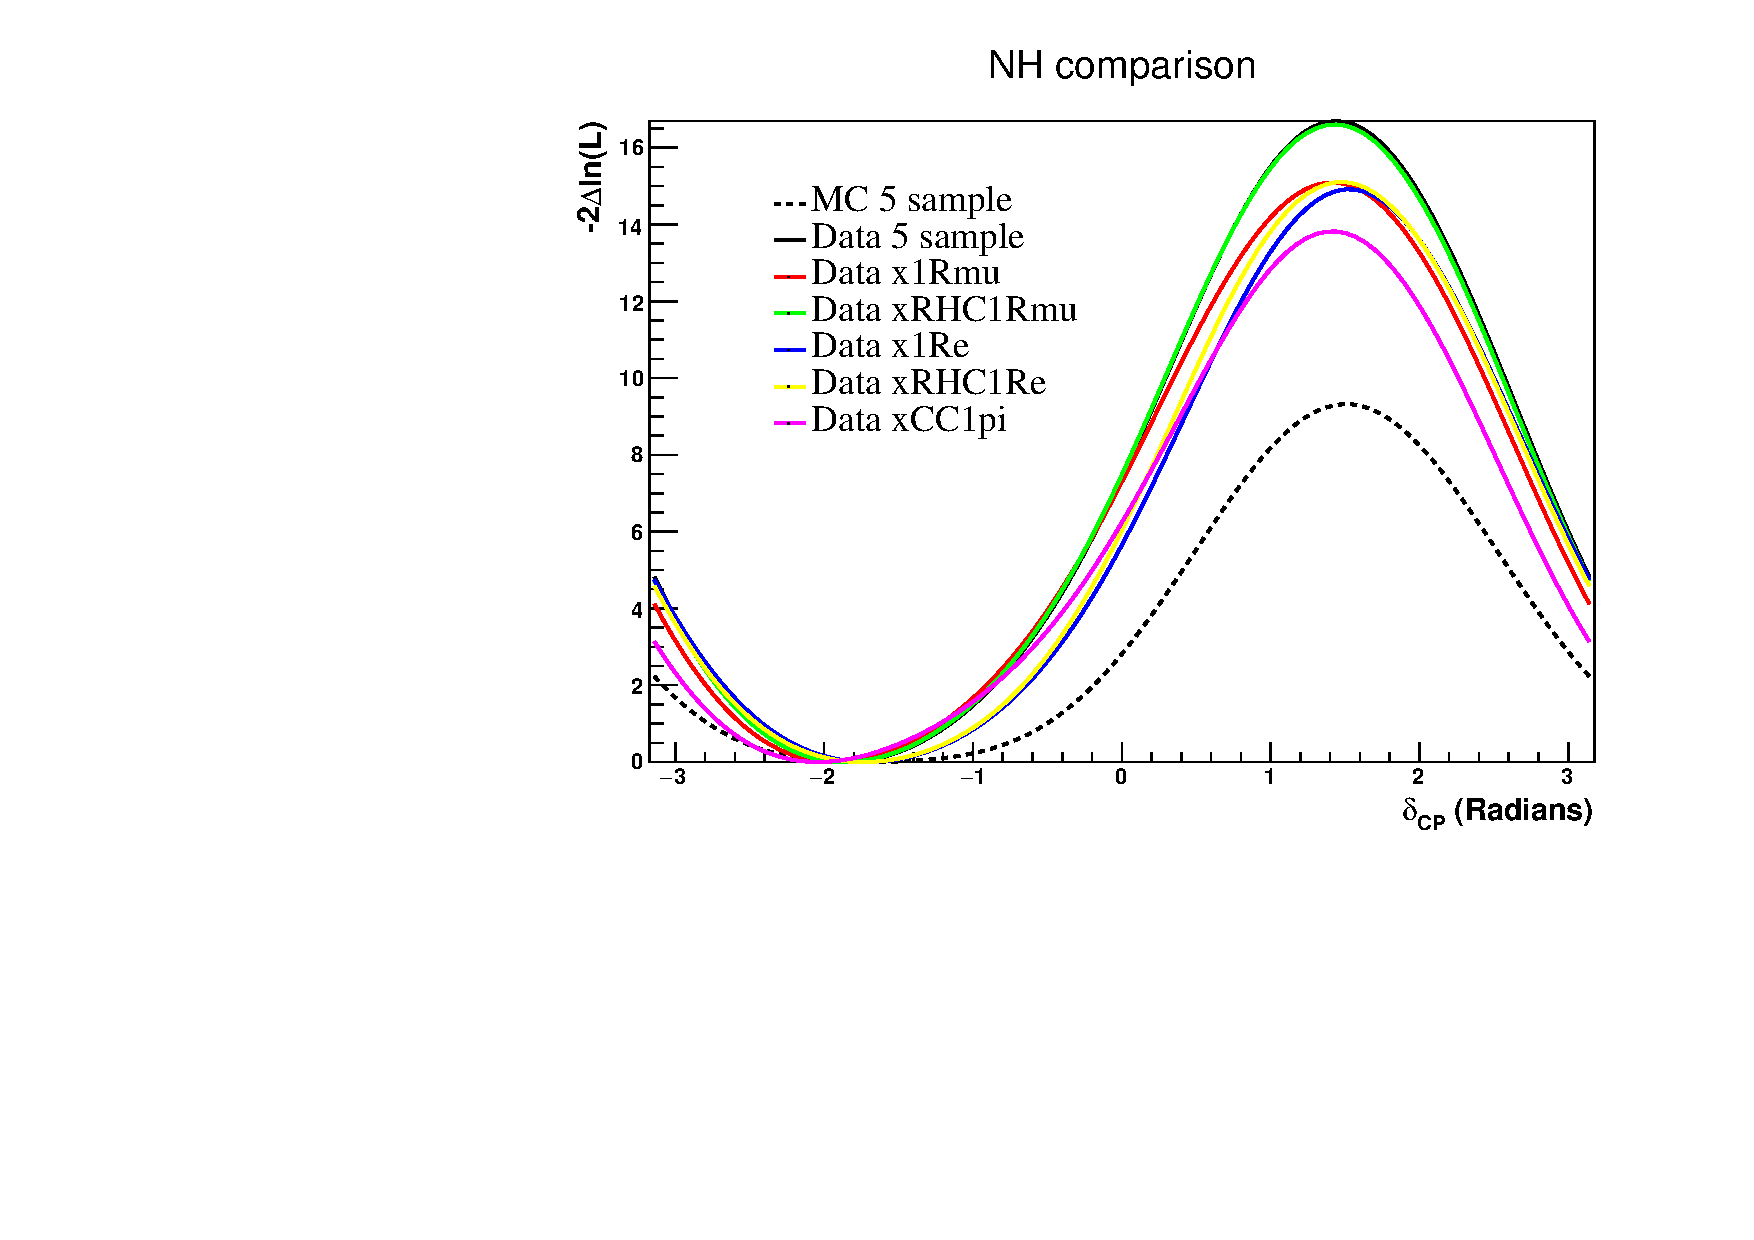
\includegraphics[width=0.9\textwidth]{studies/hybrids/deltacp_hybrids}
	\caption {
		The expected $\Delta\chi^2$ distribution as a function of \deltacp with reactor constraint for MC, data and data/MC hybrid data sets.
	}
	\label{fig:deltacp_hybrids}
\end{figure*}

% <THIS MAY BE RELEVANT COMPARING 4 SAMPLE TO 5 SAMPLE IF THE 5 SAMPLE PREFERS A LARGER THETA13 THAN THE 4 SAMPLE> The effect is also apparent in the $\sin^2 \theta_{13}$ Vs $\delta_{CP}$ contours where the new analysis prefers a larger value of $\sin^2 \theta_{13}$ which, when constrained by the reactor measurements, results in a stronger constraint on $\delta_{CP}$. 


% <AS ABOVE> The comparison of the fits to $\sin^2 \theta_{23}$ Vs $\Delta m^2_{32}$ are slightly unexpected considering the sensitivity study, however the result where a greater portion of the lower octant of $\sin^2 \theta_{23}$ is excluded at 90\%CL and 68\%CL can be explained again by the excess of events observed in the \nueCConepi{}  which favour a much larger value of $\sin^2 \theta_{23}$ and therefore push the parameter to the upper octant. \color{red}(speculative, needs confirmation)\color{black}

A stronger than expected constraint is also evident in the disappearance contour, with greater exclusion in \ssqthtwothree. Similarly to the \deltacp hybrid fits above, \cref{fig:disappearance_hybrids} shows the expected sensitivity from the Asimov A data set (red), the data fit (black) and then a number of additional fits where one of the data samples was replaced by the corresponding Asimov A sample. From this one can see that the stronger constraint can be explained by the deficit in the observed number of events in the one-ring $\mu$-like sample.

\begin{figure*}[htb]
	\center
	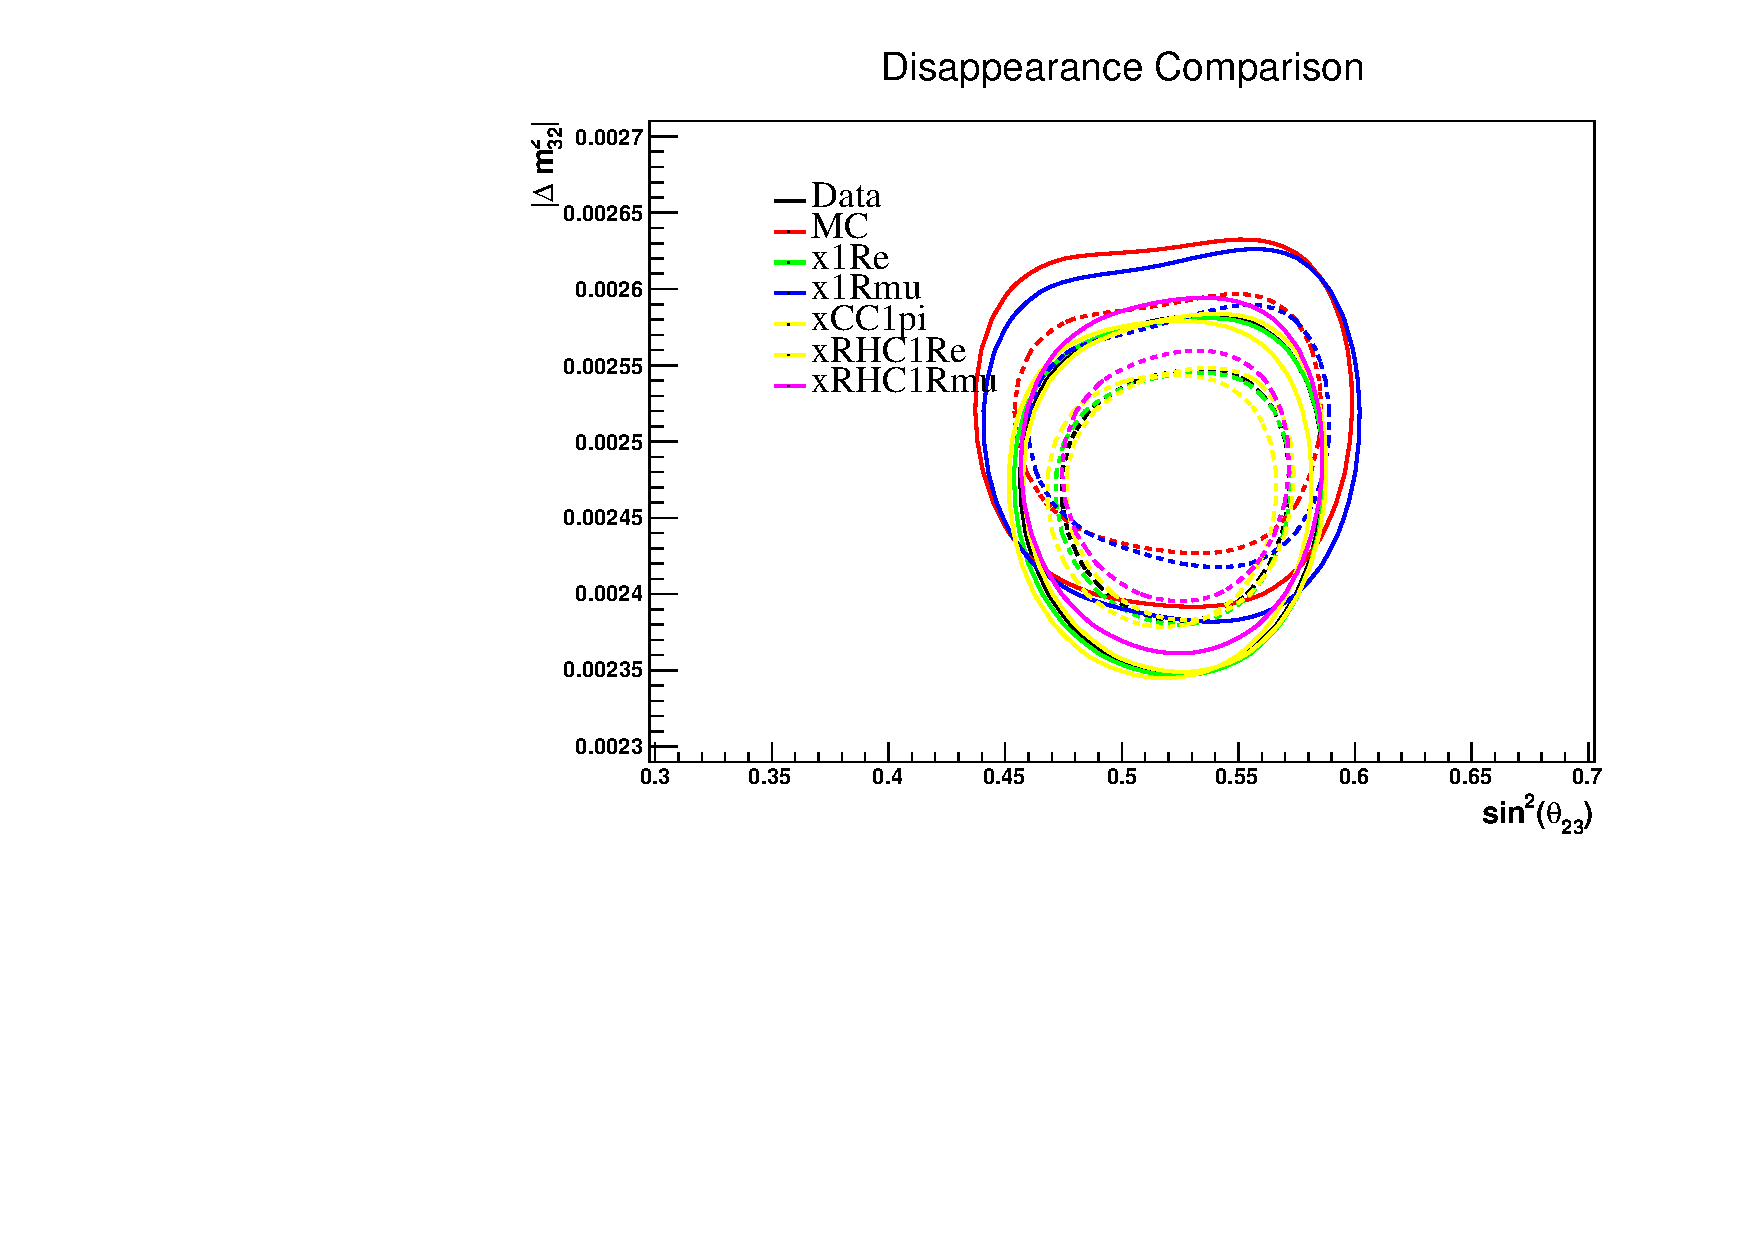
\includegraphics[width=0.9\textwidth]{studies/hybrids/disappearance_hybrids}
	\caption {
		The expected disappearance contours with reactor constraint for normal hierarchy for MC, data and data/MC hybrid data sets.
	}
	\label{fig:disappearance_hybrids}
\end{figure*}

% <AS ABOVE> The comparison of the fits to $\sin^2 \theta_{23}$ Vs $\Delta m^2_{32}$ are slightly unexpected considering the sensitivity study, however the result where a greater portion of the lower octant of $\sin^2 \theta_{23}$ is excluded at 90\%CL and 68\%CL can be explained again by the excess of events observed in the \nueCConepi{}  which favour a much larger value of $\sin^2 \theta_{23}$ and therefore push the parameter to the upper octant. \color{red}(speculative, needs confirmation)\color{black}

The value of \ssqthonethree favoured by the analysis is \BestFitMixingOneThreewoRC and corresponds to normal hierarchy, with the 1D contours in agreement with the PDG 2016 reactor constraint ($0.0219 \pm 0.0012$) at $\sim1.2 \sigma$ (see \cref{tab:data_bestfit}).

The value of \ssqthtwothree favoured by the analysis is \BestFitMixingTwoThreewRC (\BestFitMixingTwoThreewoRC) with (without) the reactor constraint and corresponds to normal hierarchy, with the 1D contours in agreement with and without the reactor constraint at $1 \sigma$, favouring maximal mixing as seen in our previous analyses.

The value of \dmsqtwothree favoured by the analysis is \BestFitDmTwoThreewRC $\times 10^{-3}\text{ eV}^2\text{/c}^4$ (\BestFitDmTwoThreewoRC$\times 10^{-3}\text{ eV}^2\text{/c}^4$) with (without) the reactor constraint and corresponds to normal hierarchy, with the 1D contours in agreement with and without the reactor constraint at $1 \sigma$.

\subsection {Comparison of \deltacp versus mass hierarchy result with sensitivity}
\label{sec:results:brazilian}

In order to provide a better understanding of the results of the \RunPeriod data fit, the result has been compared with the expected sensitivity obtained from a large number (10k) of toy experiments for different true value of \deltacp (currently only $\delta_{CP} = -\pi/2$ is included) and the mass hierarchy.

\subsubsection{Expected sensitivity method}
\label{sec:results:brazilian:method}
This section outlines the procedure to produce the expected sensitivity comparison plots. The example given is for true normal hierarchy and $\delta_{CP} = -\pi/2$.
\begin{itemize}
	\item \num{1e4} fake data sets are generated following the Feldman-Cousins method for a true value of \deltacp and mass hierarchy, in this case $\delta_{CP} = -\pi/2$ and normal hierarchy.
	\item A $\chi^2$ distribution is computed with respect to the marginalisation toys as a function of \deltacp and mass hierarchy.
	\item For each fake data set, the minimum value of $\chi^2$ for each bin of \deltacp, $\chi^2_{bin,min}$ is found with respect to both normal and inverted hierarchy.
	\item The test statistic is then computed as $\Delta\chi^2_{bin} = \chi^2_{bin} - \chi^2_{bin,min}$, which is slightly different to the Feldman-Cousins method, where $\Delta\chi^2_{FC} = \chi^2_{true} - \chi^2_{best-fit}$. The distributions of $\Delta\chi^2_{bin}$ and $\Delta\chi^2_{FC}$ coincide if the bin is $\delta_{CP} = -\pi/2$ and normal hierarchy, i.e. the true point used to generate the toy experiments.
	\item This results in a $\Delta\chi^2$ distribution from which we can draw conclusions about the expected $\Delta\chi^2$ for each value of \deltacp given a hypothesised true value and hierarchy.
	\item The spread of the $\Delta\chi^2$ distribution for each point of \deltacp and mass hierarchy is obtained as the range of the $\Delta\chi^2_{bin}$ distribution that contains respectively the 68.27\% and 95.45\% of the toy experiments on its left side. The test statistic $\Delta\chi^2_{bin}$ is assumed ot be 1-sided because by construction $\chi^2_{bin,min} \le \chi^2_{bin}$.
	\item An alternative to the one-sided distribution is also produced, for which values of $\Delta\chi^2$ of each bin of \deltacp are themselves binned (100 evenly-spaced bins on the range [$\Delta\chi^2_{bin,min},\Delta\chi^2_{bin,max}$]) and then toys are added to the expected sensitivity bands starting from the bin of $\Delta\chi^2$ that contains the most toys, until 68.27\% and 95.45\% of the toy experiments have been included, thereby producing two-sided distributions.
	\item A plot is also produced to show the fraction of toy experiments which exclude each value of \deltacp to greater than $2\sigma$ significance in the Feldman-Cousins corrected critical values along with the probabilities to exclude $\delta_{CP} = 0$ and $\delta_{CP} = \pi$ for a given true value of \deltacp.
\end{itemize}

\subsubsection{$\delta_{CP} = -\pi/2$ - normal hierarchy}

In \cref{fig:brazilian_dcp_mpi2} the \RunPeriod data result for \deltacp versus mass hierarchy is compared to the $1\sigma$ and $2\sigma$ uncertainties on the $\Delta\chi^2$ distributions corresponding to $\delta_{CP} = -\pi/2$ and (a) normal hierarchy and (b) inverted hierarchy. We see that the data contour is contained within the $2\sigma$ band for inverted hierarchy, whilst the data contour falls just outside the $2\sigma$ band for normal hierarchy in the region around $\delta_{CP} = 0$. This suggests that the data constraint is consistent with the PMNS matrix at around the $2\sigma$ level.

We also see an interesting feature near $\delta_{CP} = -\pi/2$ where the $\Delta\chi^2$ values have a wider distribution. This is due to the boundary at $\delta_{CP} = -\pi/2$ which causes a wider distribution when the parameter \deltacp would like to be pushed beyond the boundary in the fit.

Finally from \cref{fig:brazilian_dcp_mpi2}(c) we see that $\delta_{CP} = 0$ and $\delta_{CP} = \pi$ are excluded at 90\% confidence level in around 40\% (see \cref{tab:exclusion_prob}) of the toy experiments and excluded at $2\sigma$ confidence level in between 25\% and 30\% of the toy experiments, with $\delta_{CP} = \pi$ excluded in slightly fewer toy experiments in each case.

\begin{figure*}[htb]
	\center
	\begin{subfigure}[b]{0.49\textwidth}
		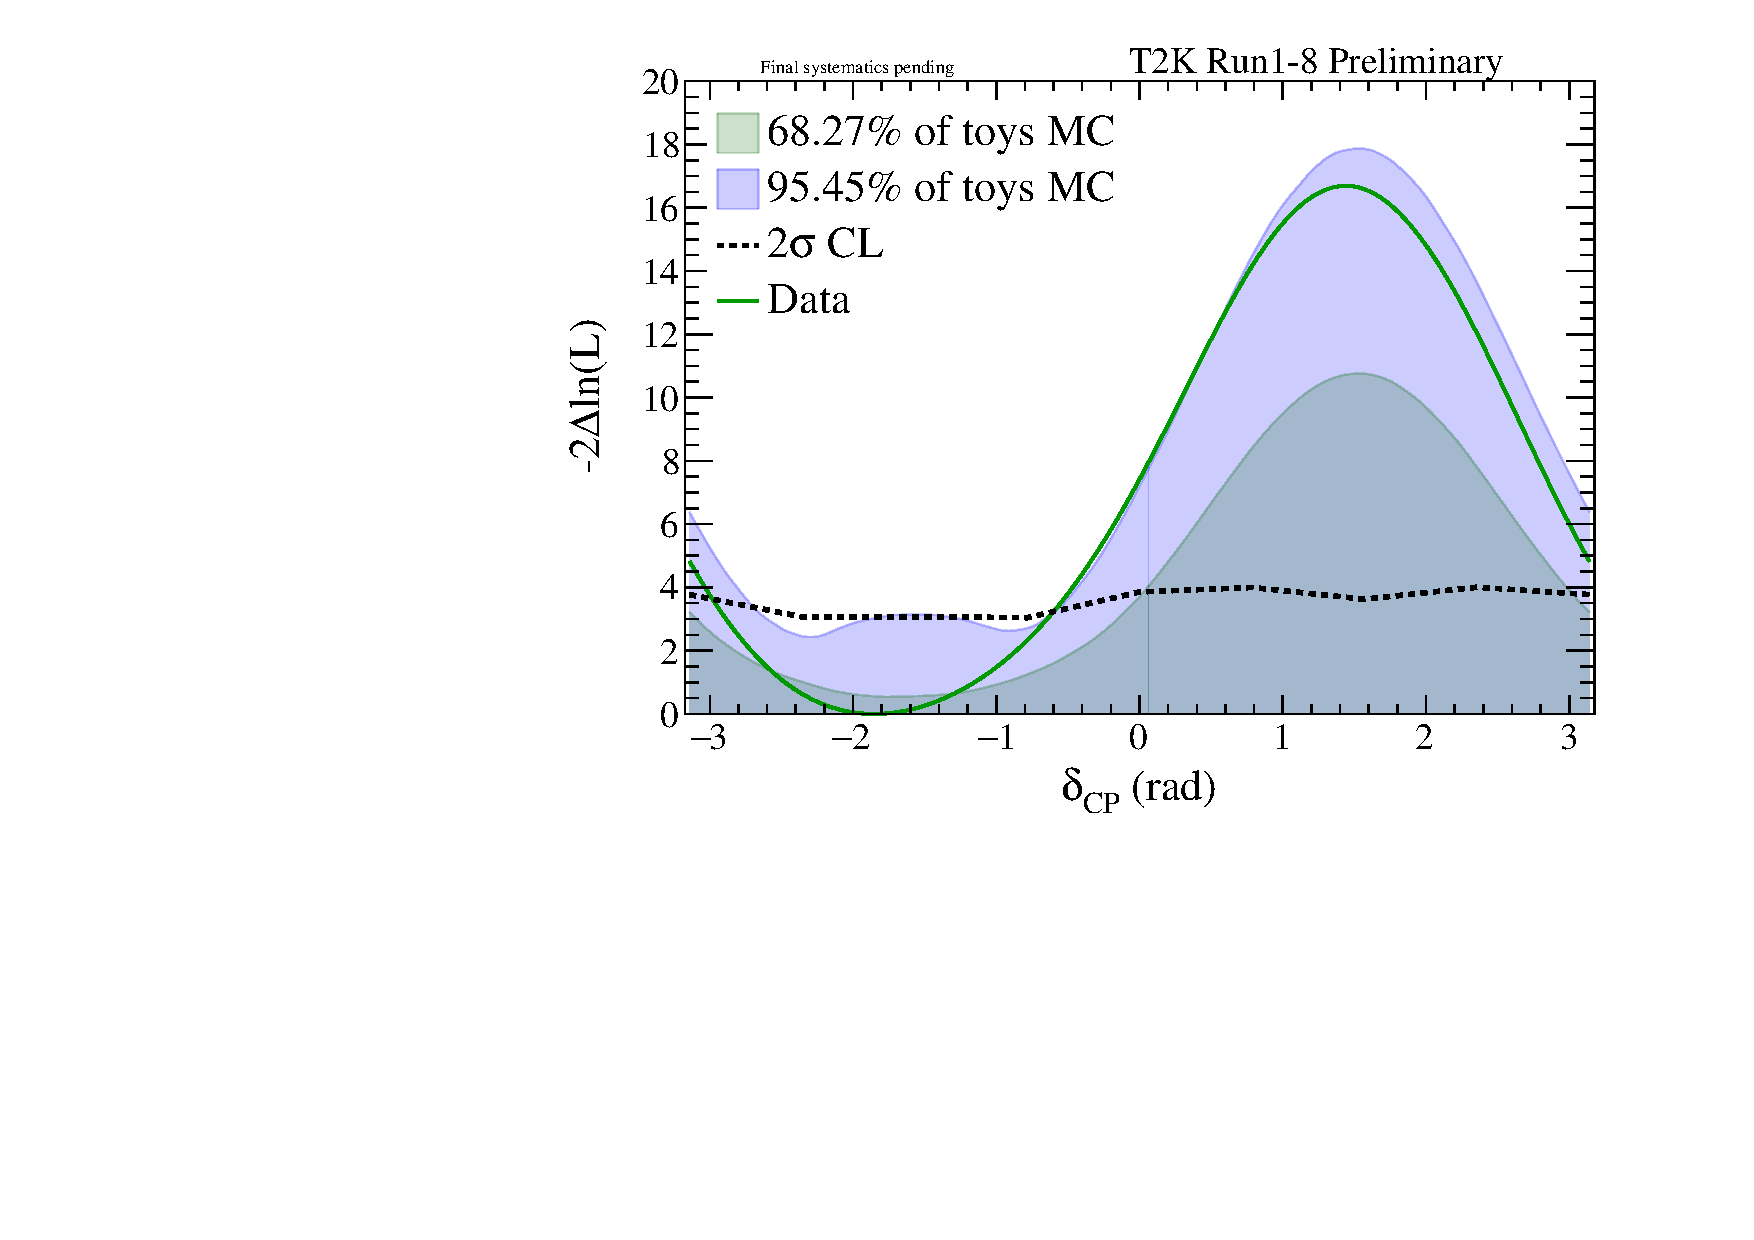
\includegraphics[width=0.9\textwidth]{comparison/dcp_run18_react_Data_braz_nh}
		\caption{Normal hierarchy}
	\end{subfigure}
	\begin{subfigure}[b]{0.49\textwidth}
		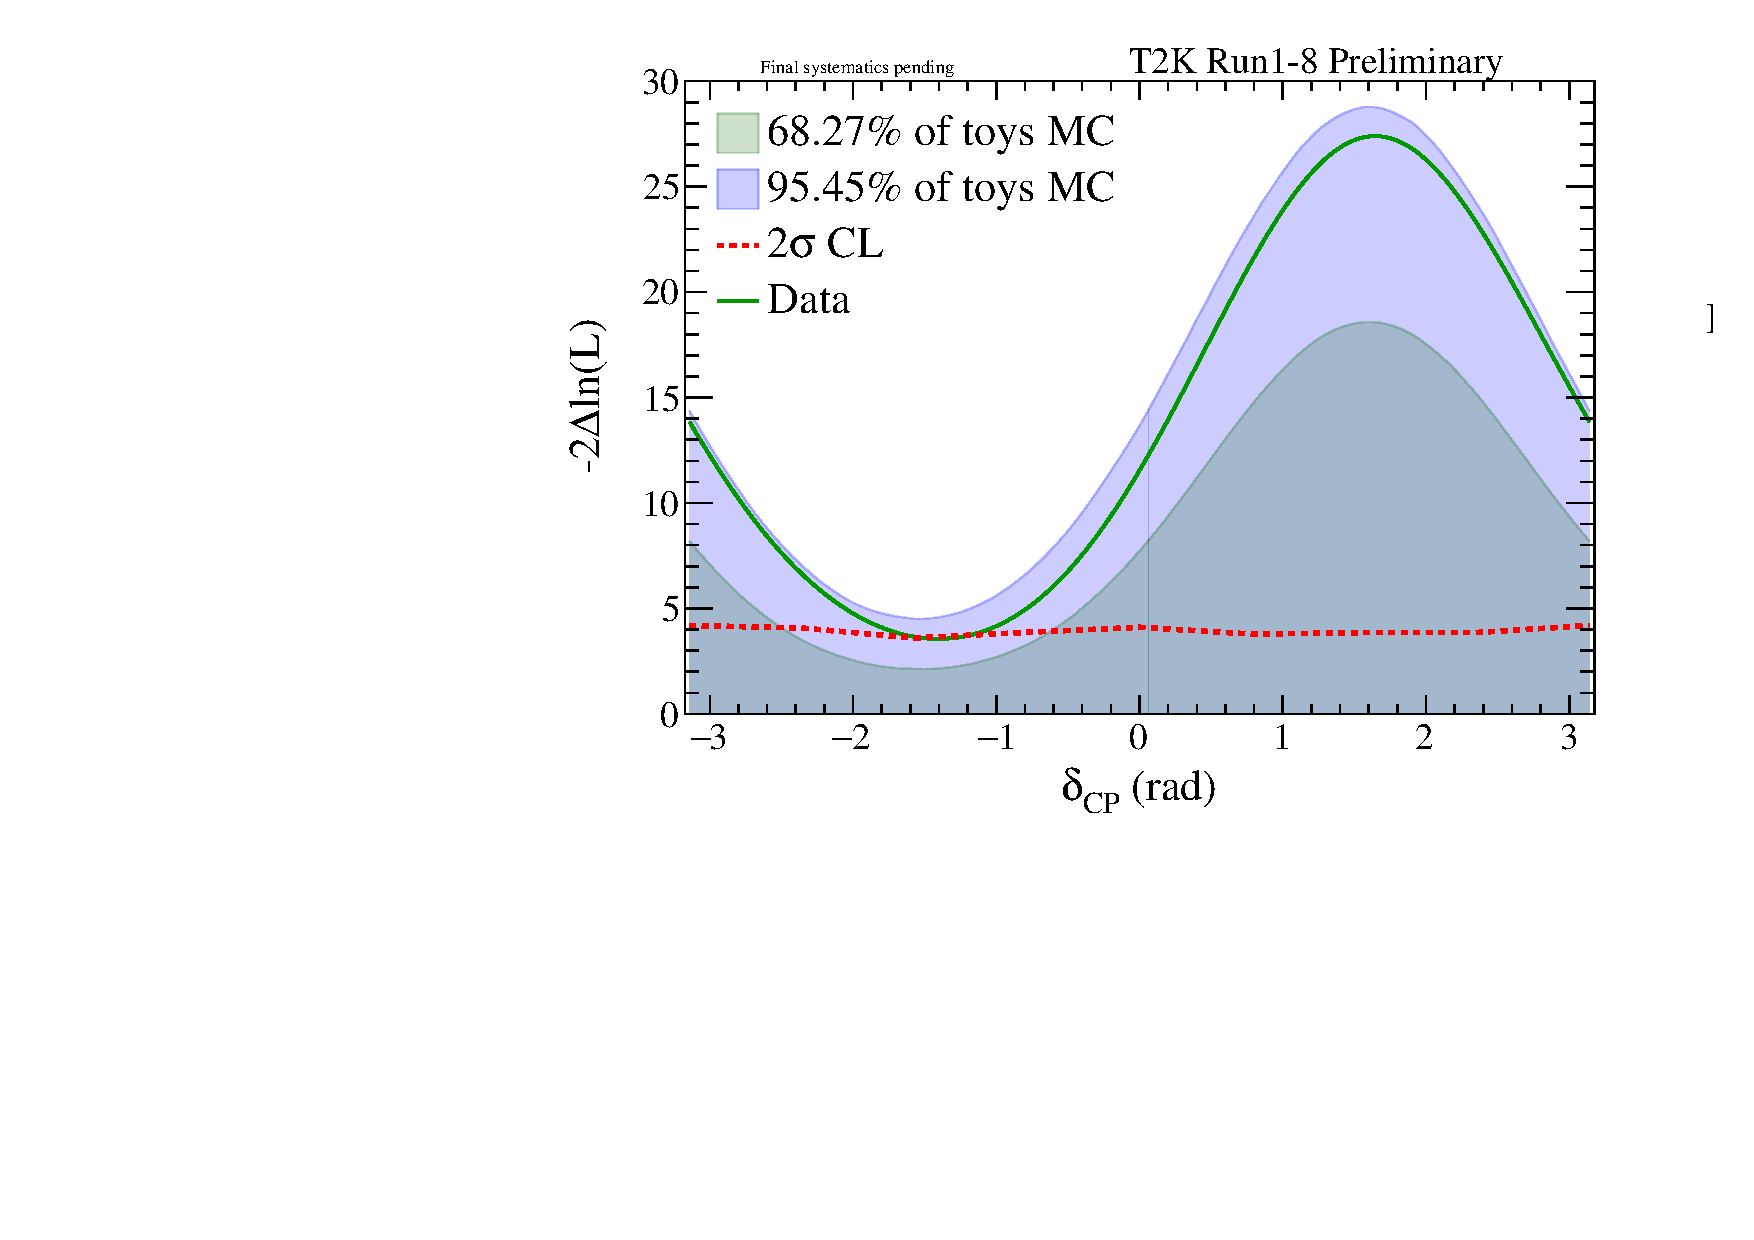
\includegraphics[width=0.9\textwidth]{comparison/dcp_run18_react_Data_braz_ih}
		\caption{Inverted hierarchy}
	\end{subfigure}
	\begin{subfigure}[b]{0.49\textwidth}
		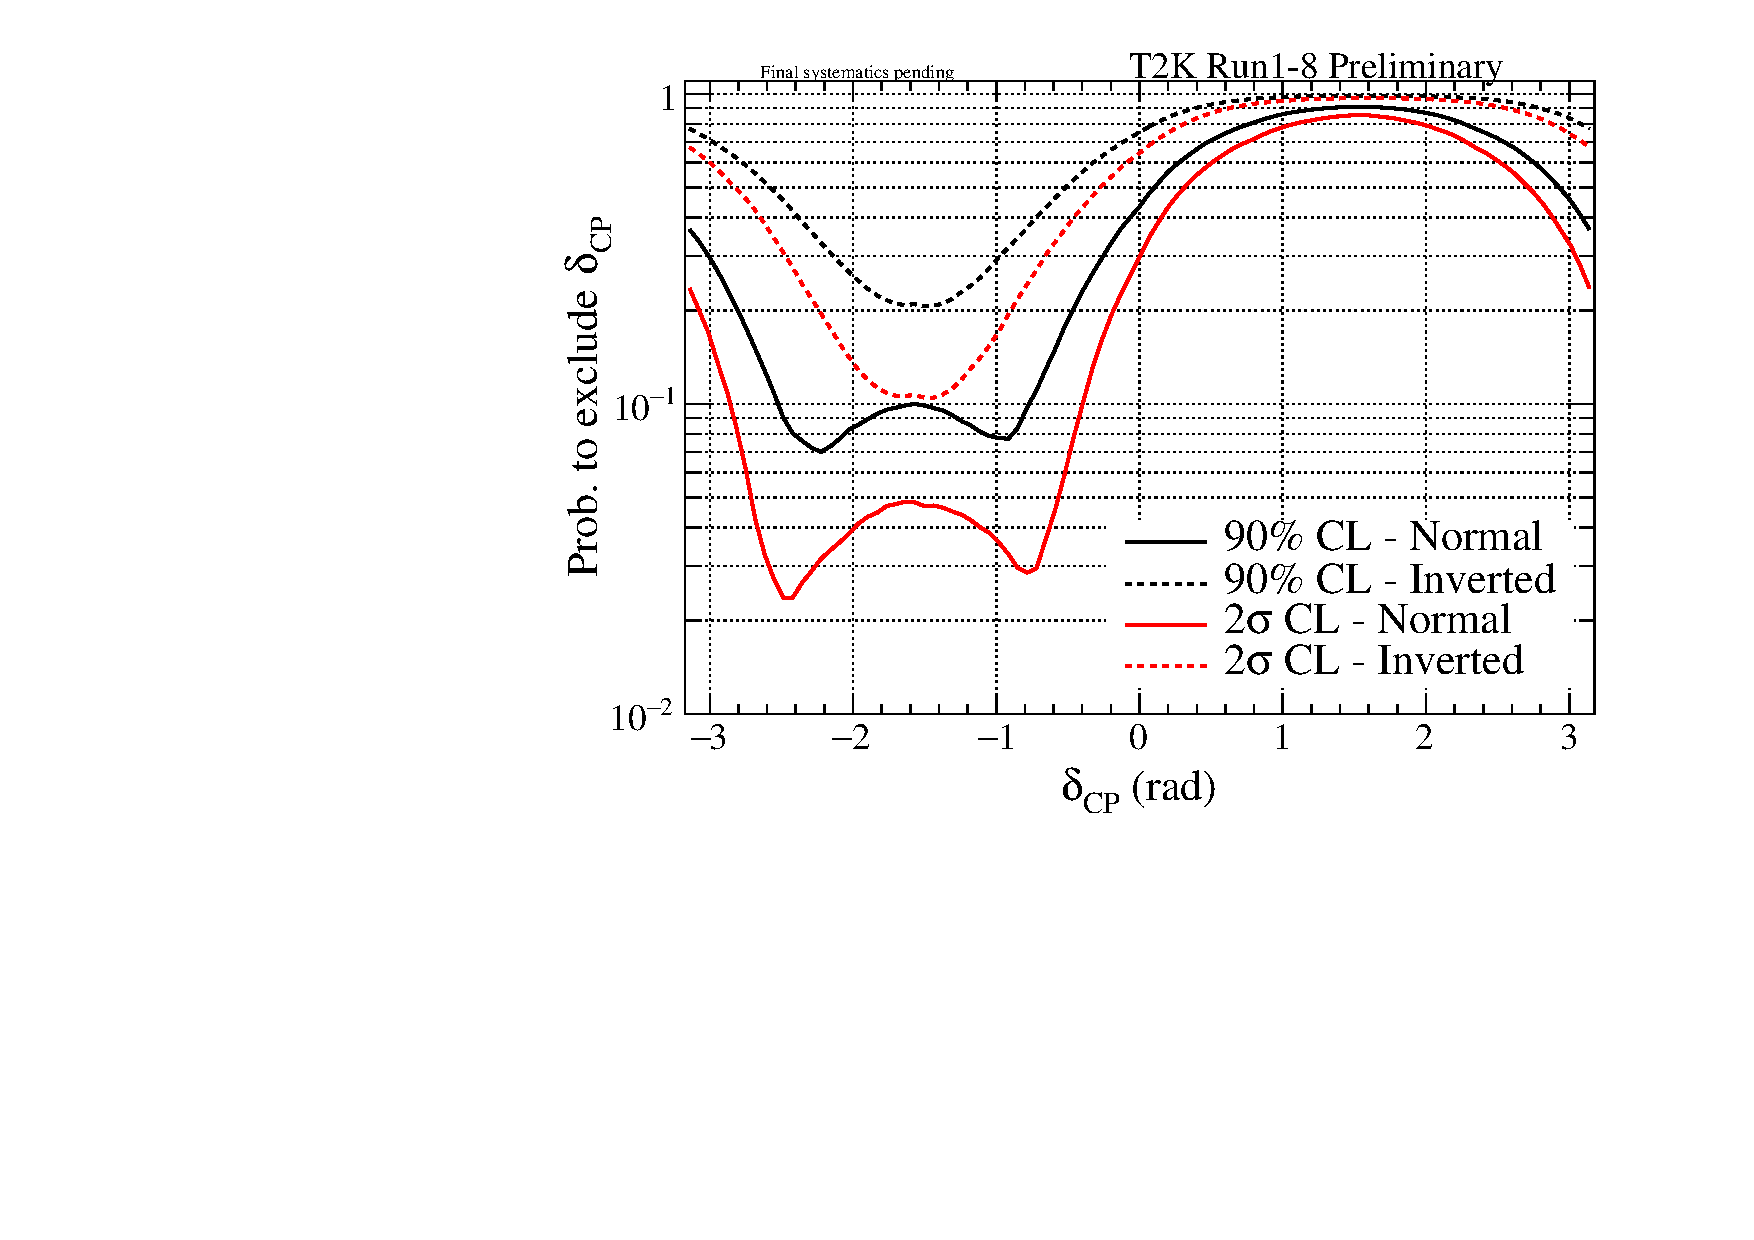
\includegraphics[width=0.9\textwidth]{comparison/dcp_run18_react_Data_prob_chisq}
		\caption{Data \(\Delta \chi^2\) probablility }
	\end{subfigure}
	\caption {
		The distribution of $\Delta\chi^2$ vs \deltacp obtained with \num{1e4} toy experiments generated with $\delta_{CP} = -\pi/2$ and normal hierarchy is shown. The $\Delta\chi^2$ distributions obtained by fixing the mass hierarchy to normal (left) and inverted (right) are shown, along with the $\Delta\chi^2$ values corresponding to 68.27\% and 95.45\% of the toy experiments and the average $\Delta\chi^2$ values from all experiments. Also shown are the fractions of toys which exclude each value of \deltacp to 90\% and $2\sigma$ using the Feldman-Cousins corrected critical values (bottom).
	}
	\label{fig:brazilian_dcp_mpi2}
\end{figure*}

\begin{table}[htb]
	\centering
	\begin{tabular}{| c | c | c | c |}
\hline
\deltacp & Hierarchy & 90\% & $2\sigma$ \\
\hline
0		& NH & 0.430 & 0.300 \\
$\pi$	& NH & 0.383 & 0.250 \\
0		& IH & 0.760 & 0.656 \\
$\pi$	& IH & 0.769 & 0.667 \\
\hline
\end{tabular}

	\caption{
		The fraction of toy experiments for which $\delta_{CP} = 0, \pi$ and normal and inverted hierarchy are excluded at 90\% and $2\sigma$ CL is shown. 10k toy experiments are used.
	}
	\label{tab:exclusion_prob}
\end{table}

\subsubsection{$\delta_{CP} = -1.833$ - normal hierarchy}

In \cref{fig:brazilian_dcp_bestfit} the \RunPeriod data result for \deltacp versus mass hierarchy is compared to the $1\sigma$ and $2\sigma$ uncertainties on the $\Delta\chi^2$ distributions corresponding to $\delta_{CP} = -1.833$ and (a) normal hierarchy and (b) inverted hierarchy. We see that the data contour is consistent with the PMNS matrix at around the $2\sigma$ level.

\begin{figure*}[htb]
	\center
	\begin{subfigure}[b]{0.49\textwidth}
		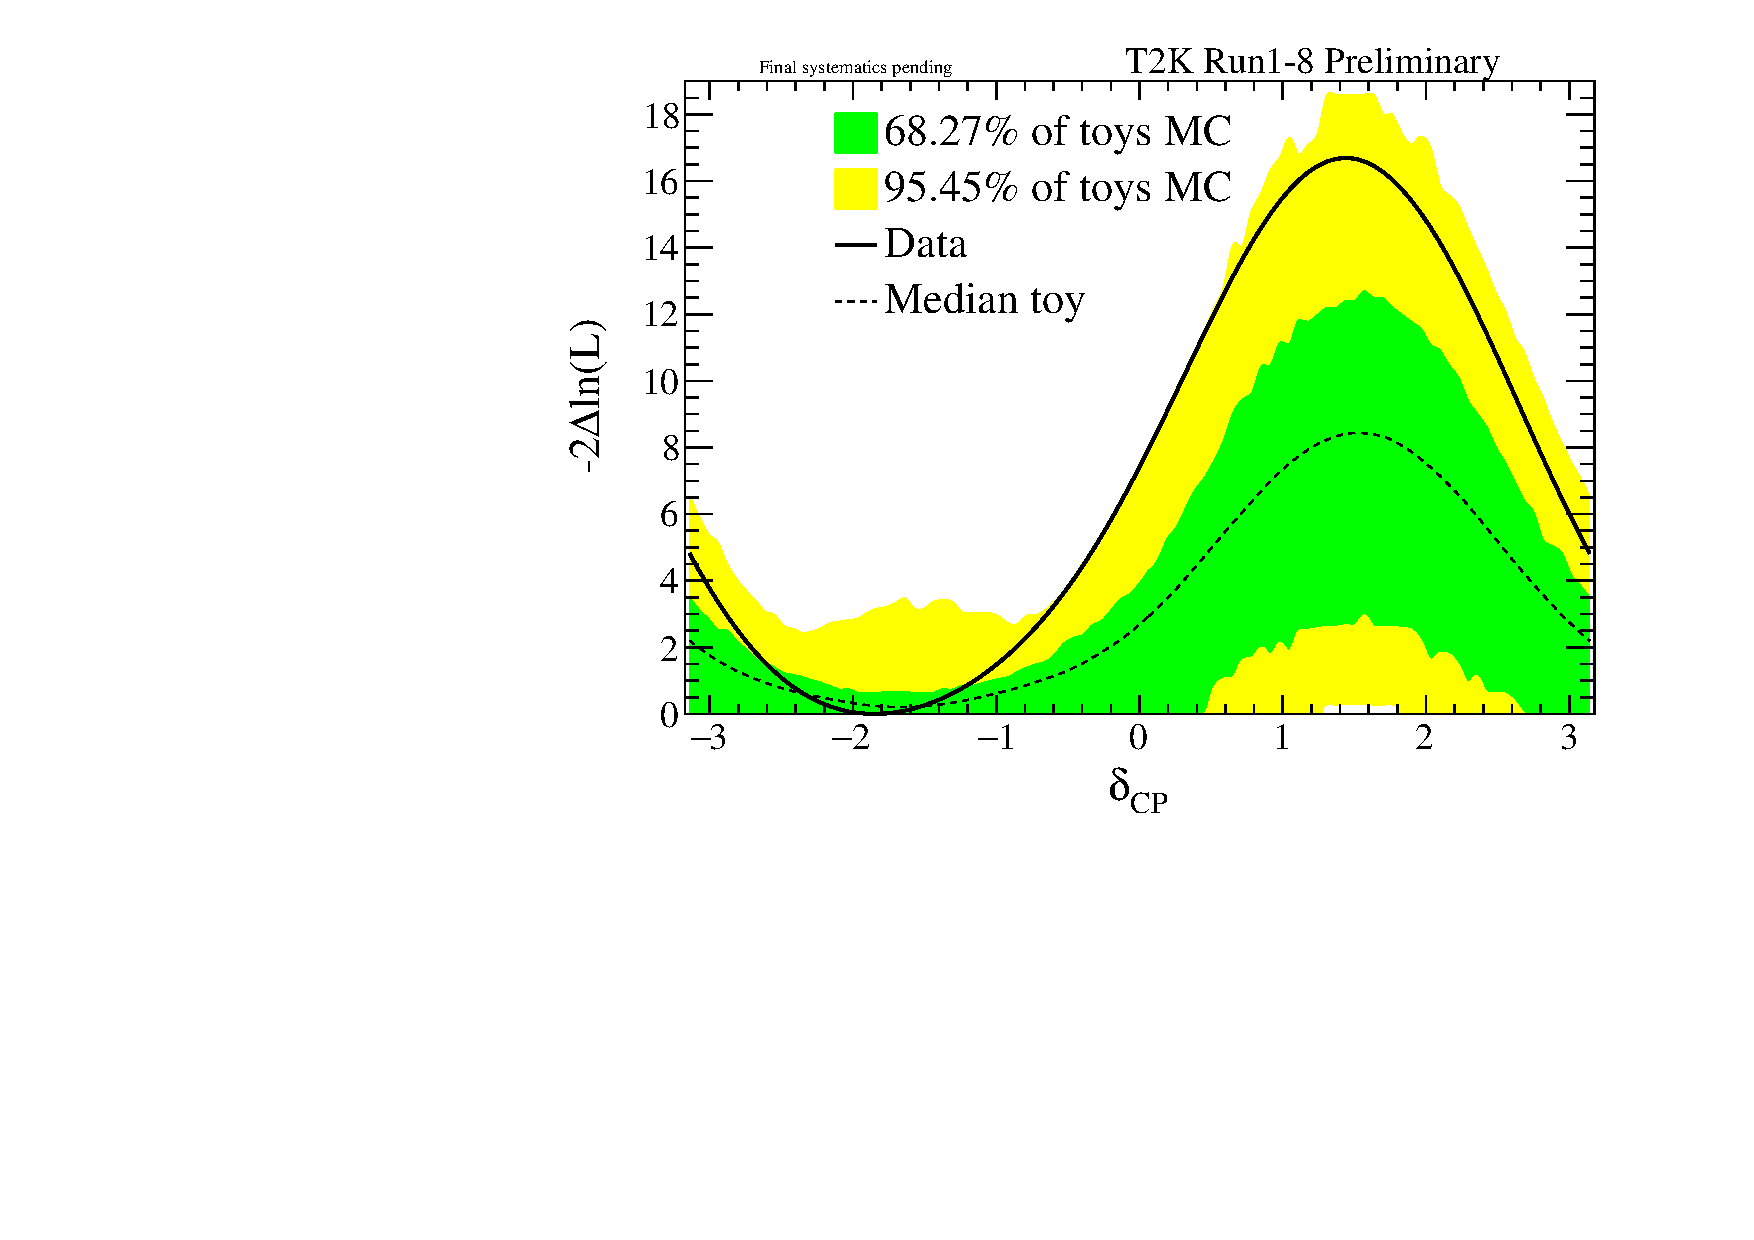
\includegraphics[width=0.9\textwidth]{comparison/deltacp/deltacp_run18_all_twosided_braz_nh}
		\caption{Normal hierarchy}
	\end{subfigure}
	\begin{subfigure}[b]{0.49\textwidth}
		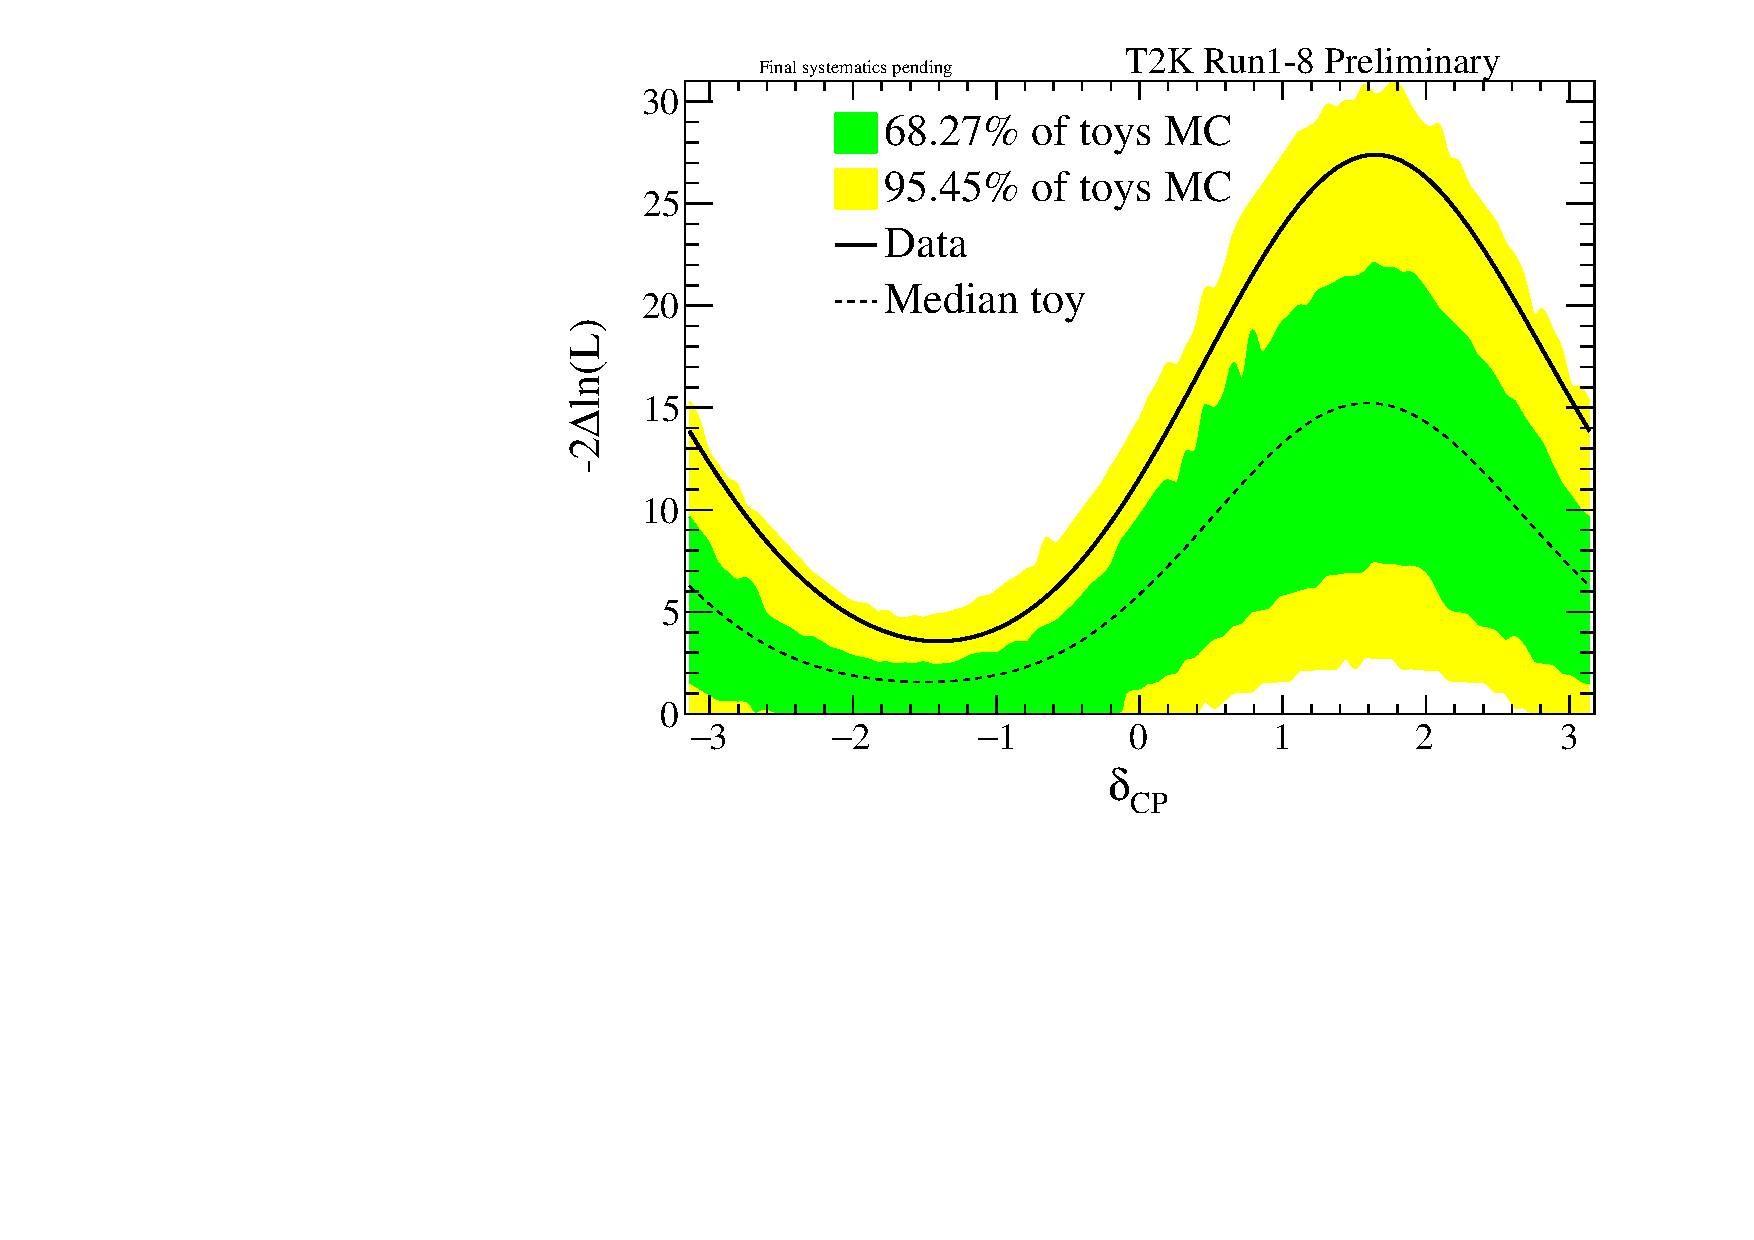
\includegraphics[width=0.9\textwidth]{comparison/deltacp/deltacp_run18_all_twosided_braz_ih}
		\caption{Inverted hierarchy}
	\end{subfigure}
	\caption {
		The distribution of $\Delta\chi^2$ vs \deltacp obtained with \num{1e4} toy experiments generated with $\delta_{CP} = -1,833$ and normal hierarchy is shown. The $\Delta\chi^2$ distributions obtained by fixing the mass hierarchy to normal (left) and inverted (right) are shown, along with the $\Delta\chi^2$ values corresponding to 68.27\% and 95.45\% of the toy experiments, the median toy and the data contour.
	}
	\label{fig:brazilian_dcp_bestfit}
\end{figure*}

\subsubsection{Sample-by-sample expected sensitivity}

An extension to the two-sided method described above was applied in order to assess the effect of each sample on the \deltacp contour obtained. There key difference to the two-sided method described in \cref{sec:results:brazilian:method} is that the generation of the \num{1e4} fake data sets is undertaken for a single sample of interest, with the remaining 4 samples being fixed at the observed spectra.

\Crefrange{fig:brazilian_dcp_nh_samples}{fig:brazilian_dcp_ih_samples}

\begin{figure*}[htb]
	\center
	\begin{subfigure}[b]{0.49\textwidth}
		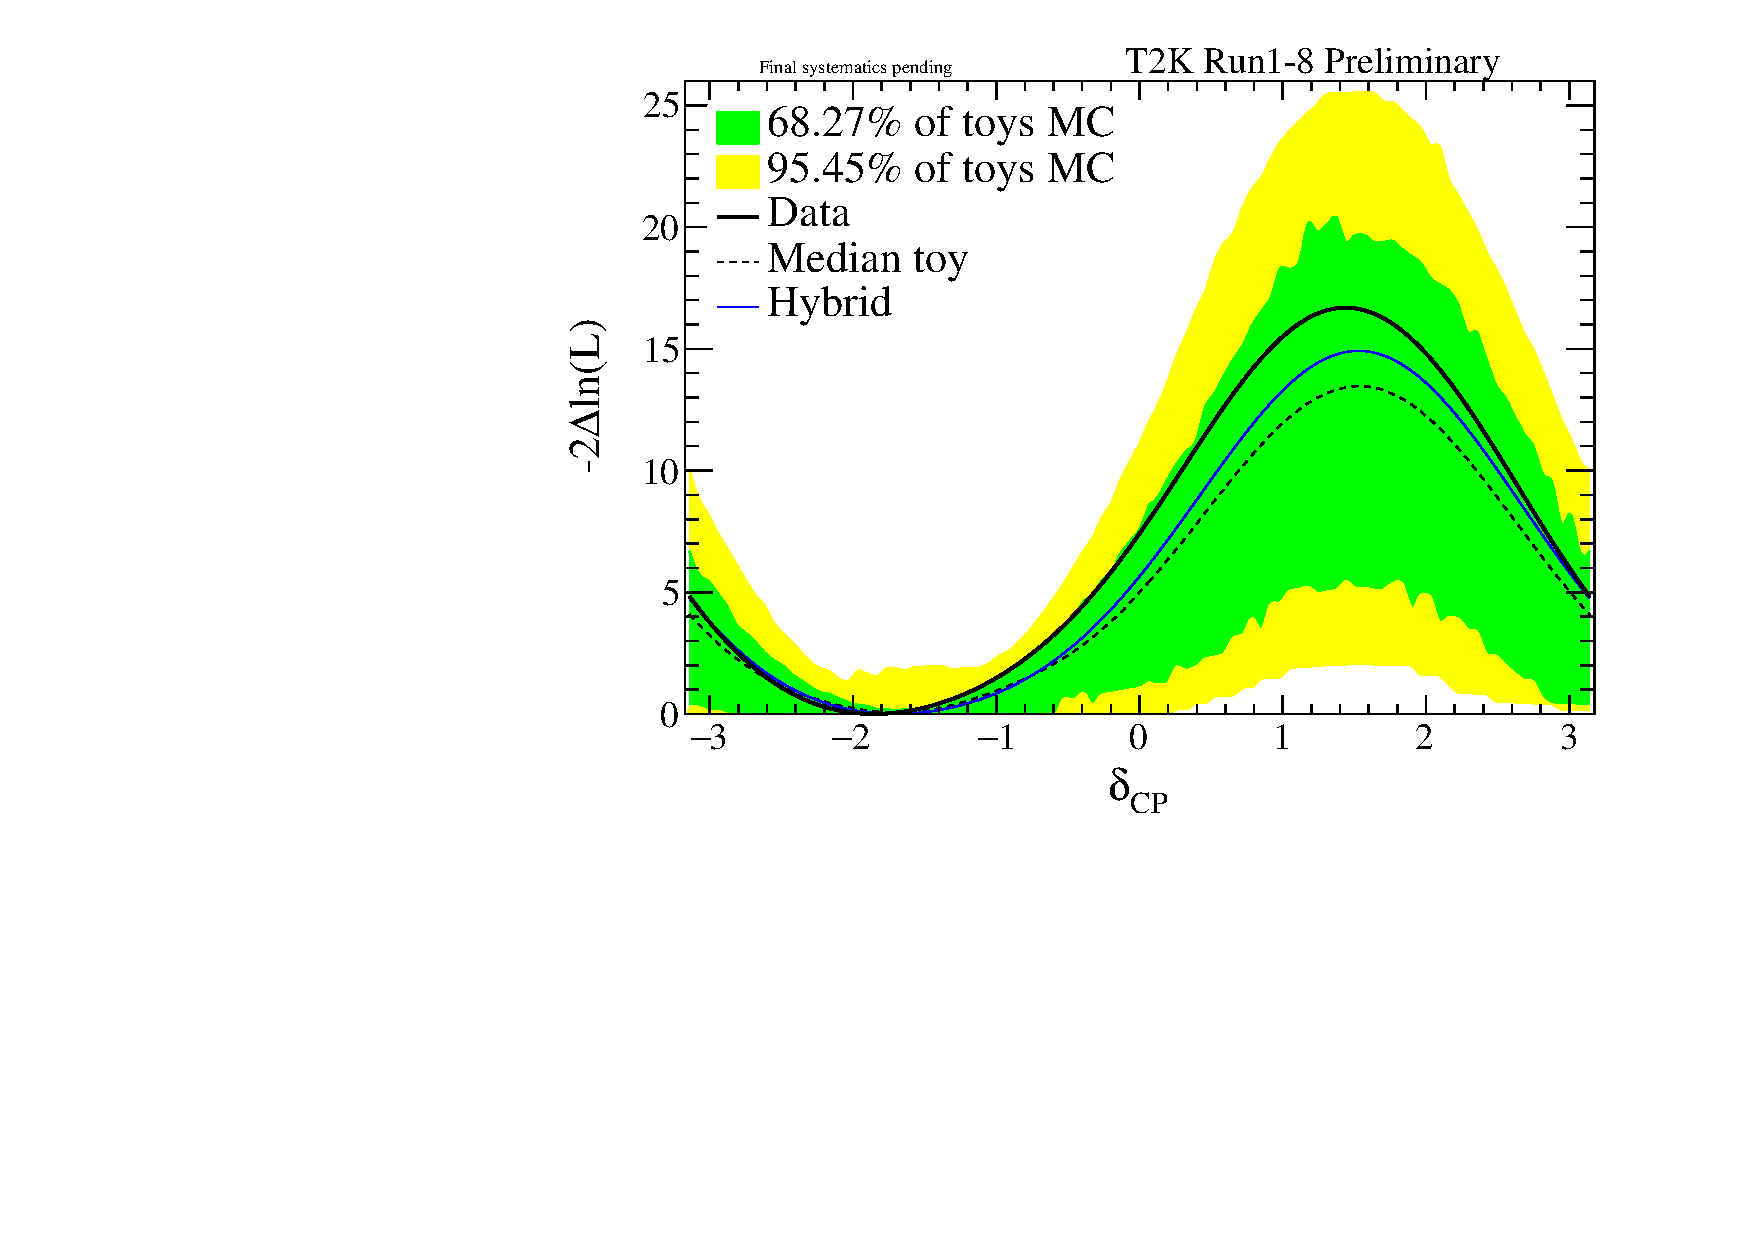
\includegraphics[width=0.9\textwidth]{comparison/deltacp_run18_fhc1re_braz_nh}
		\caption{Electron-like, neutrino mode}
	\end{subfigure}
	\begin{subfigure}[b]{0.49\textwidth}
		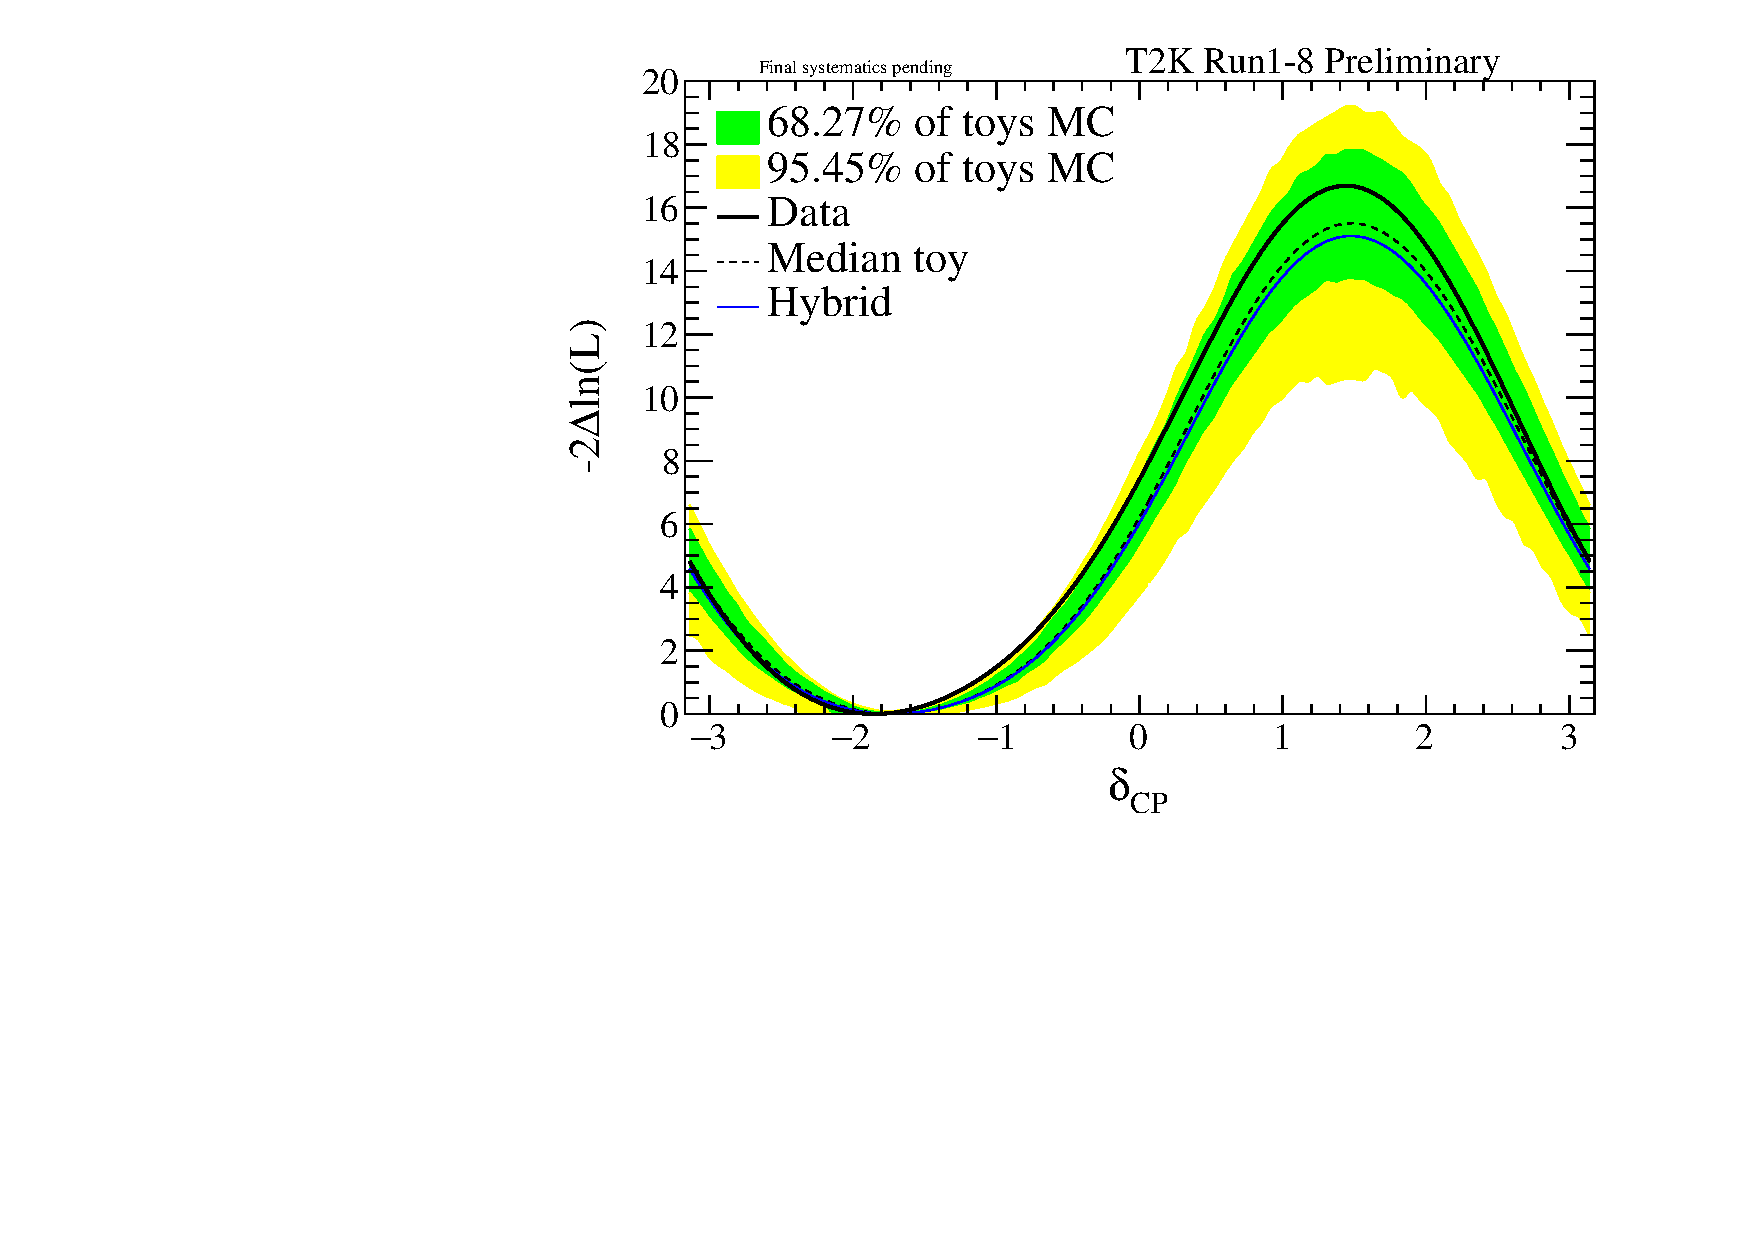
\includegraphics[width=0.9\textwidth]{comparison/deltacp_run18_rhc1re_braz_nh}
		\caption{Electron-like, antineutrino mode}
	\end{subfigure}
	\begin{subfigure}[b]{0.49\textwidth}
		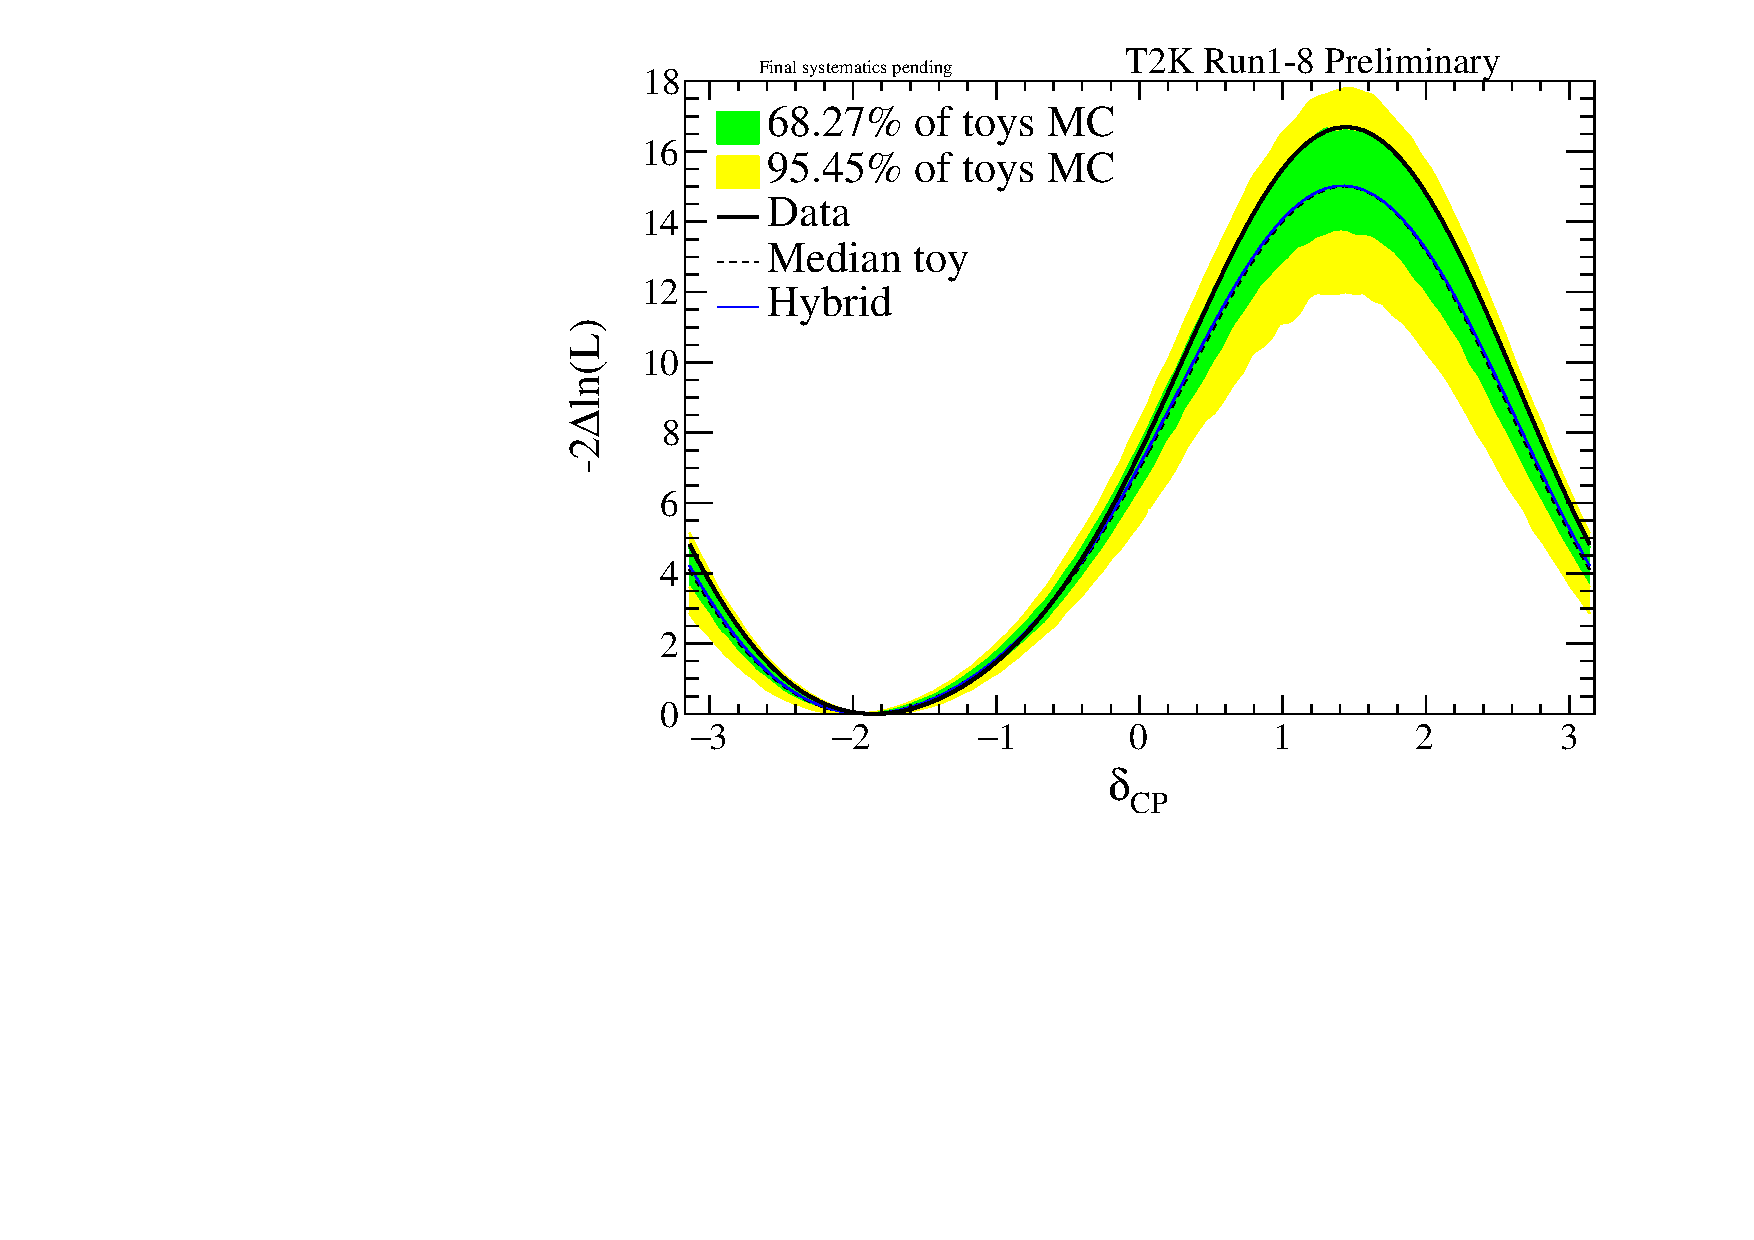
\includegraphics[width=0.9\textwidth]{comparison/deltacp_run18_fhc1rmu_braz_nh}
		\caption{Muon-like, neutrino mode}
	\end{subfigure}
	\begin{subfigure}[b]{0.49\textwidth}
		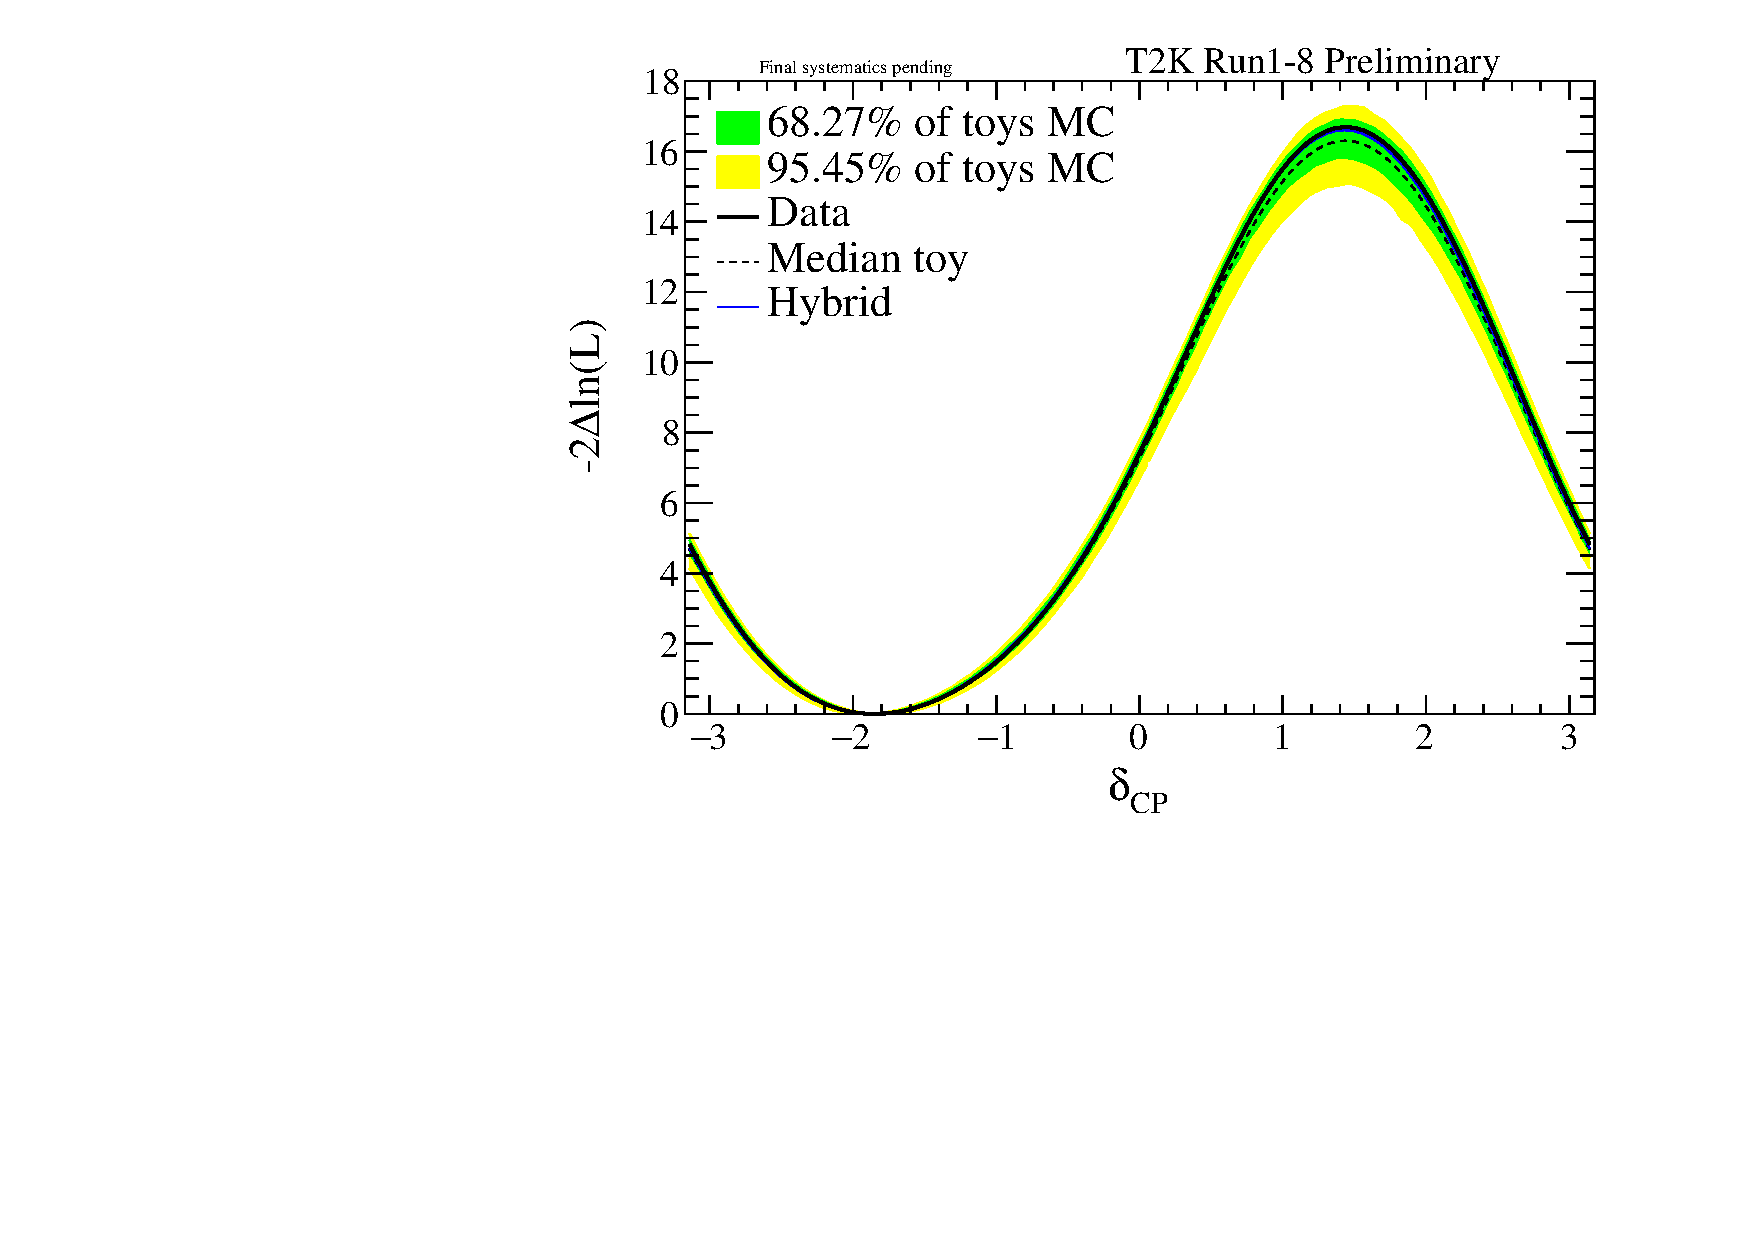
\includegraphics[width=0.9\textwidth]{comparison/deltacp_run18_rhc1rmu_braz_nh}
		\caption{Muon-like, antineutrino mode}
	\end{subfigure}
	\begin{subfigure}[b]{0.49\textwidth}
		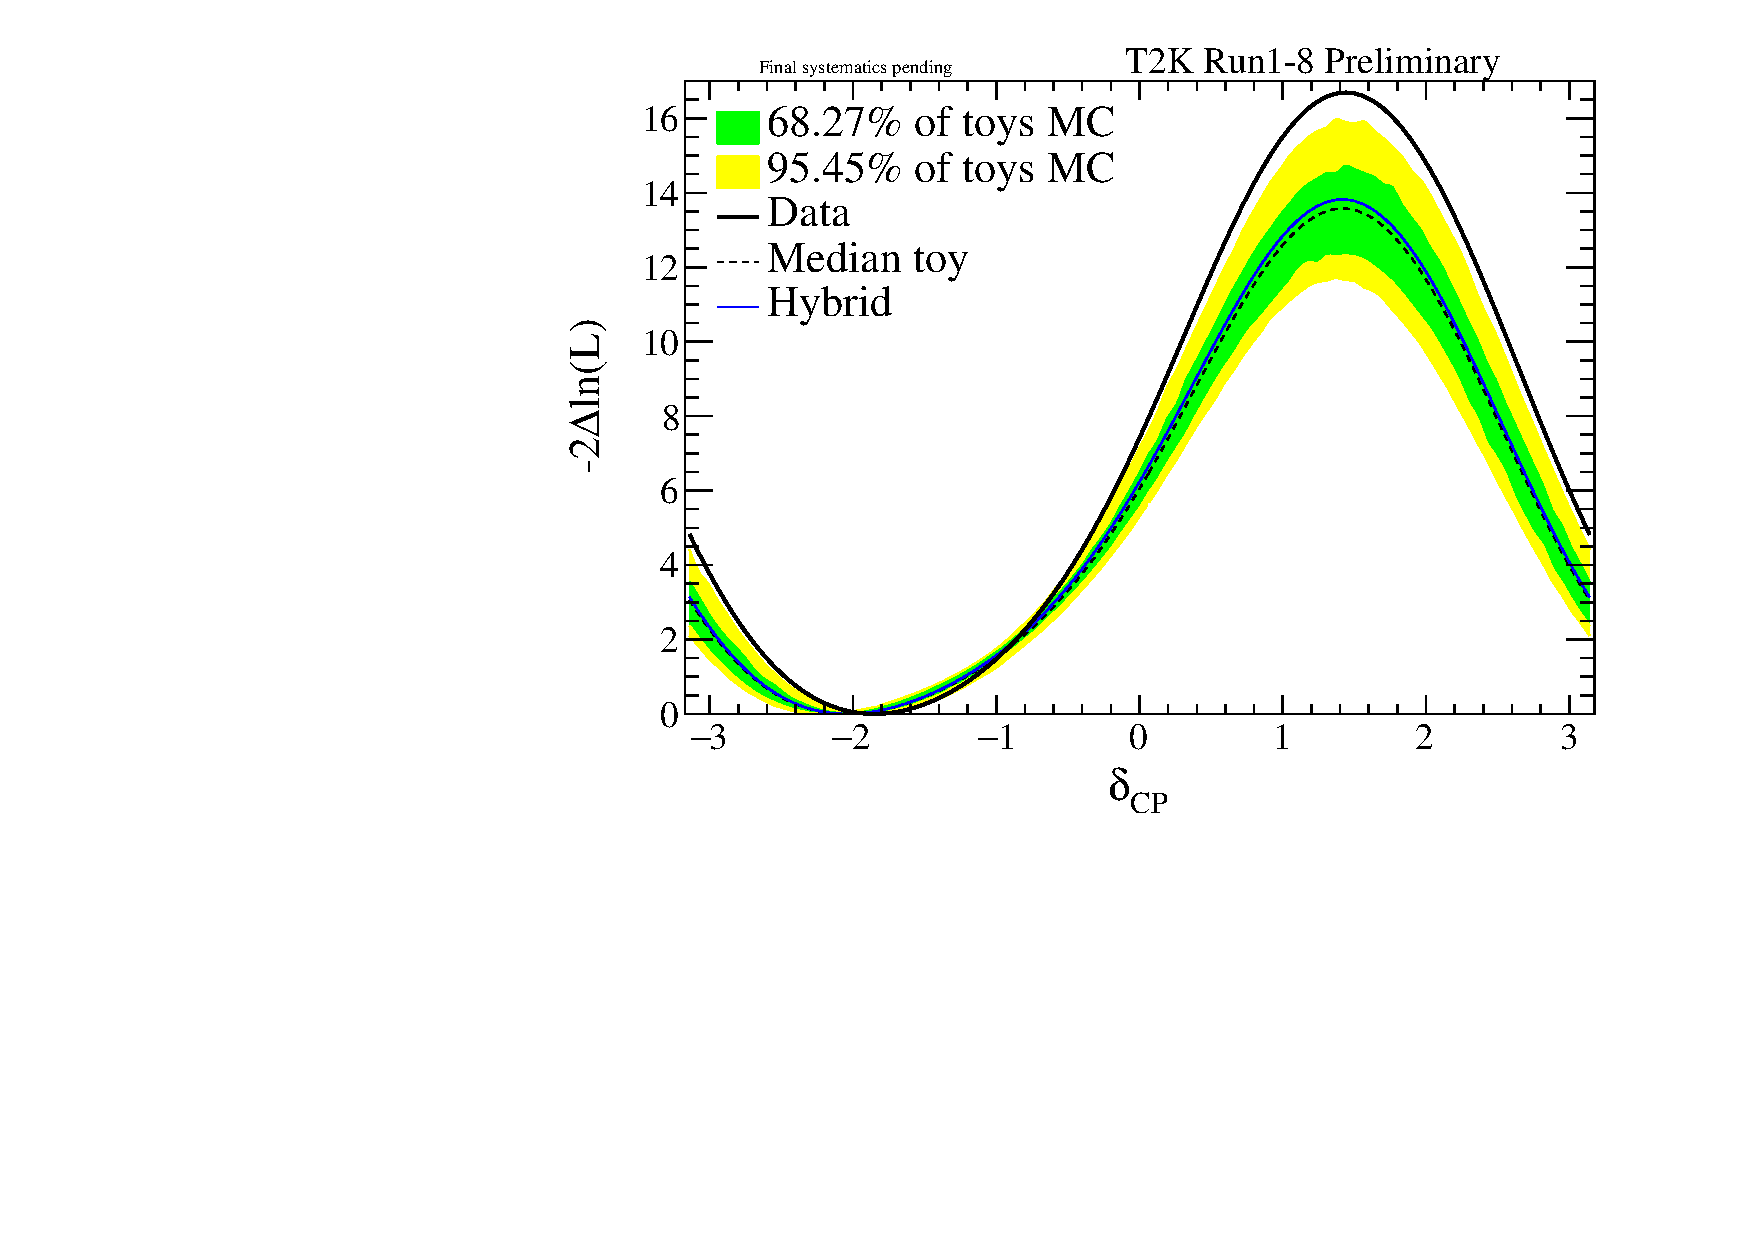
\includegraphics[width=0.9\textwidth]{comparison/deltacp_run18_cc1pi_braz_nh}
		\caption{\nueCConepi-like, neutrino mode}
	\end{subfigure}
	\caption {
		The distribution of $\Delta\chi^2$ vs \deltacp obtained with \num{1e4} toy experiments generated with $\delta_{CP} = -1.833$ and normal hierarchy is shown. The $\Delta\chi^2$ distribution obtained from the full 5-sample fit, obtained by fixing the mass hierarchy to normal, is shown, along with the $\Delta\chi^2$ values corresponding to 68.27\% and 95.45\% of the toy experiments for the indicated sample, with all other samples fixed at their observed spectra.
	}
	\label{fig:brazilian_dcp_nh_samples}
\end{figure*}

\begin{figure*}[htb]
	\center
	\begin{subfigure}[b]{0.49\textwidth}
		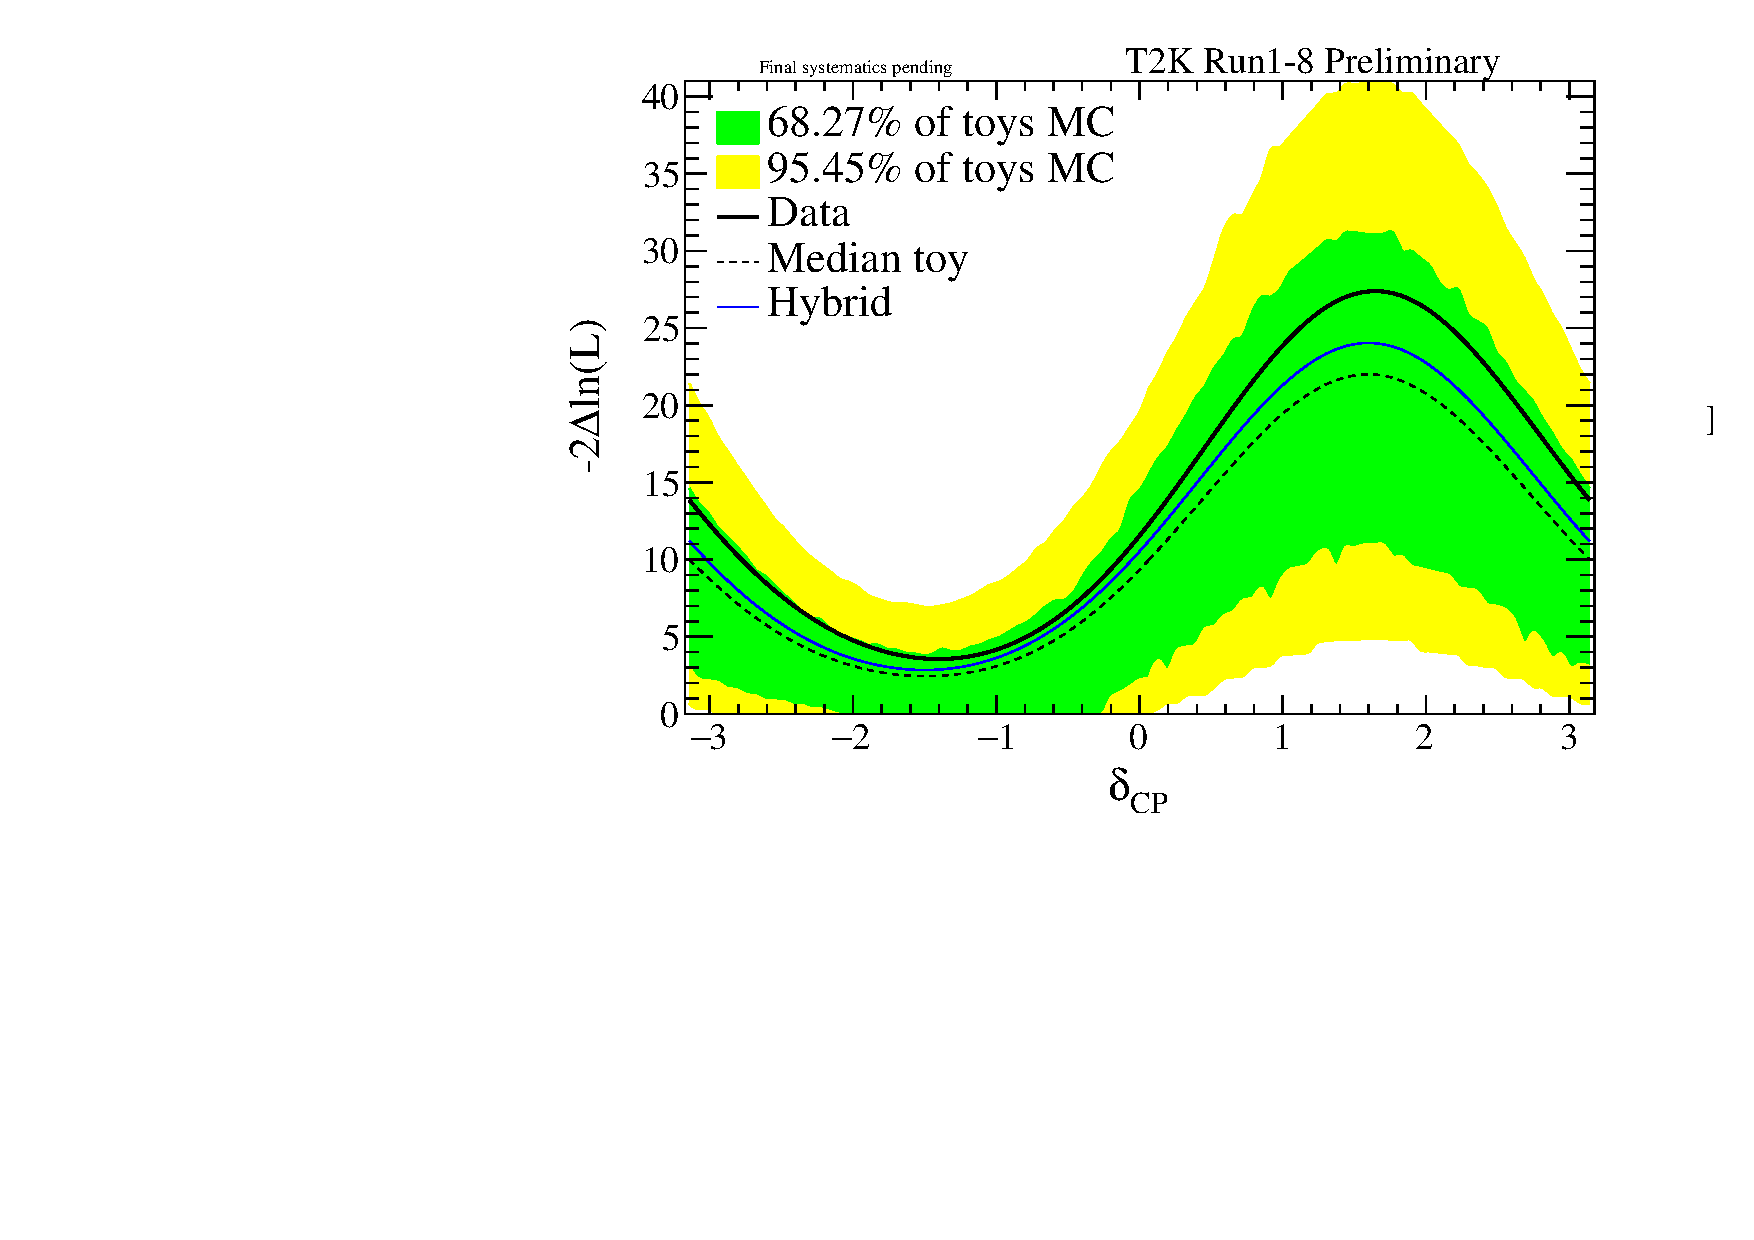
\includegraphics[width=0.9\textwidth]{comparison/deltacp_run18_fhc1re_braz_ih}
		\caption{Electron-like, neutrino mode}
	\end{subfigure}
	\begin{subfigure}[b]{0.49\textwidth}
		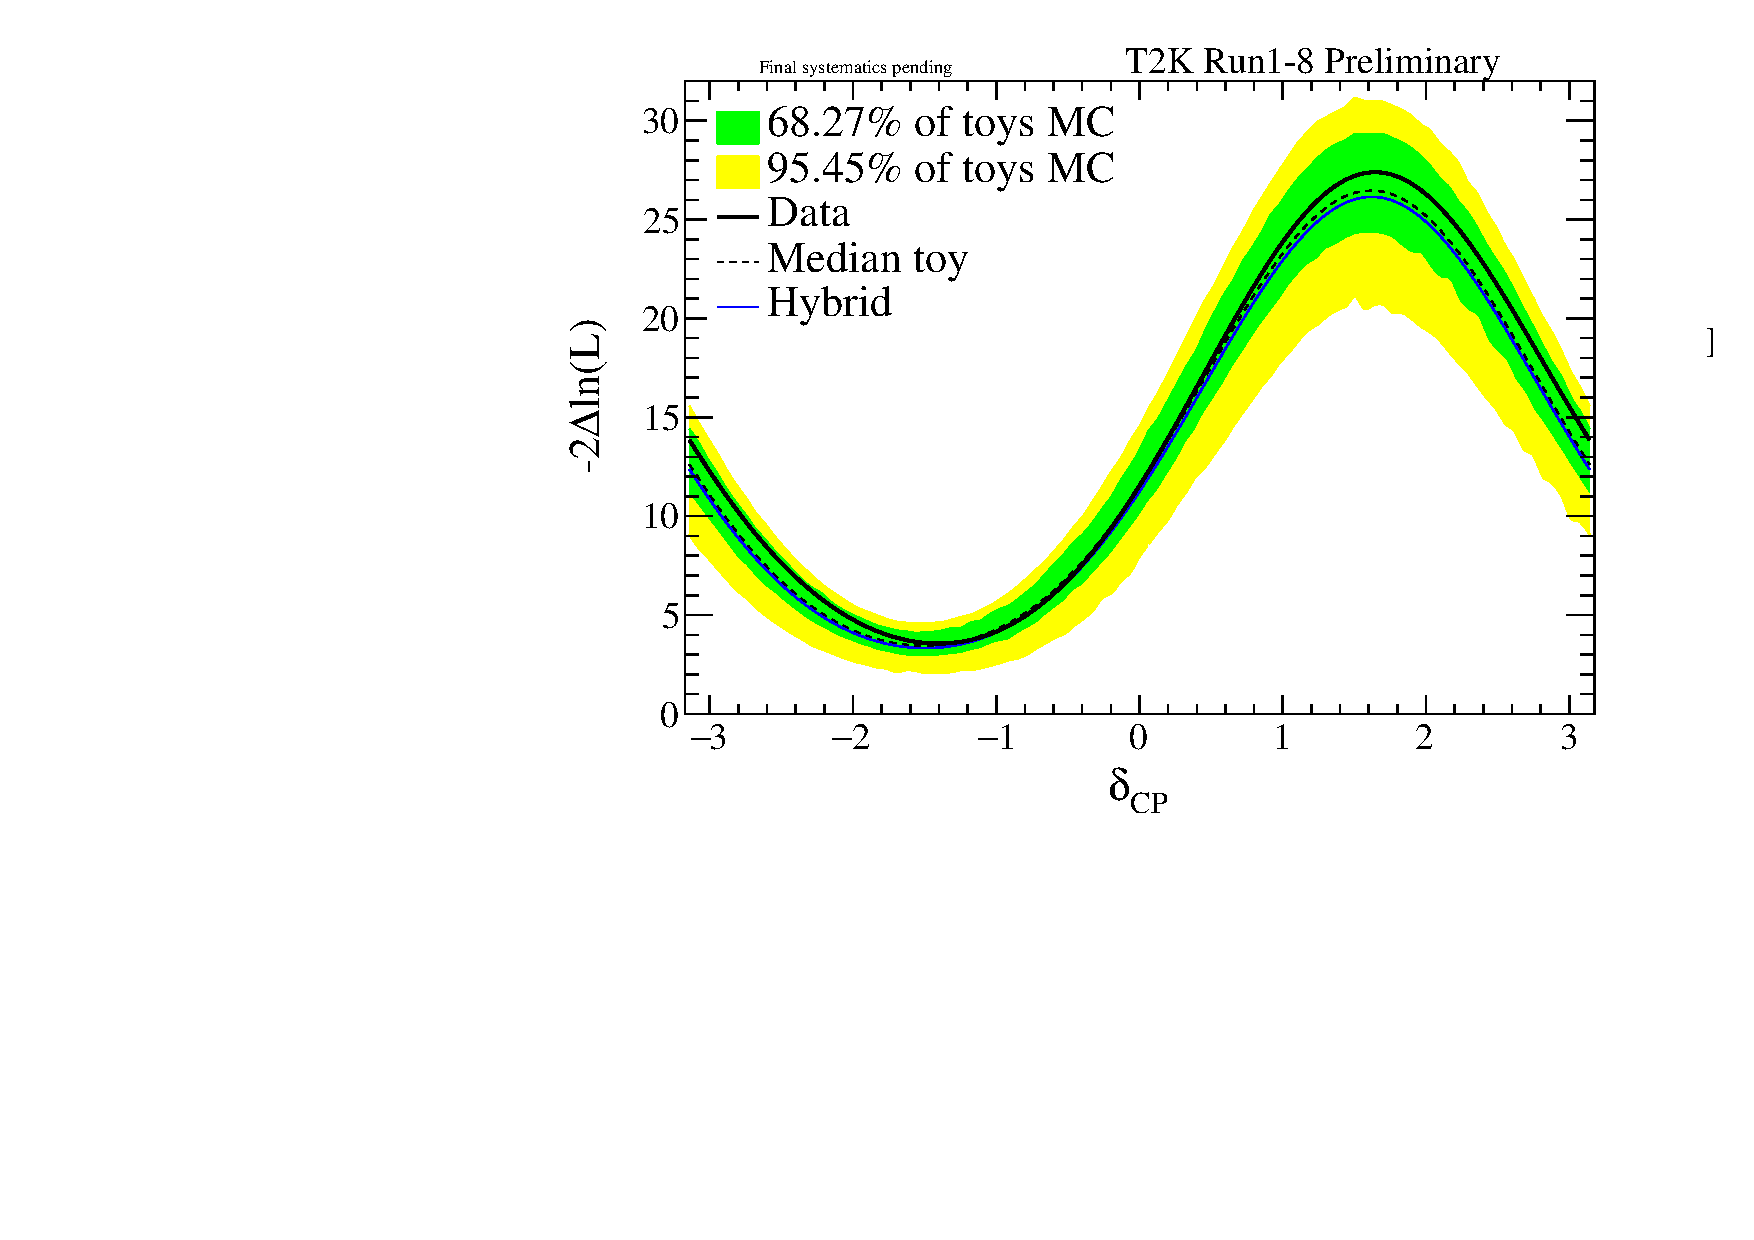
\includegraphics[width=0.9\textwidth]{comparison/deltacp_run18_rhc1re_braz_ih}
		\caption{Electron-like, antineutrino mode}
	\end{subfigure}
	\begin{subfigure}[b]{0.49\textwidth}
		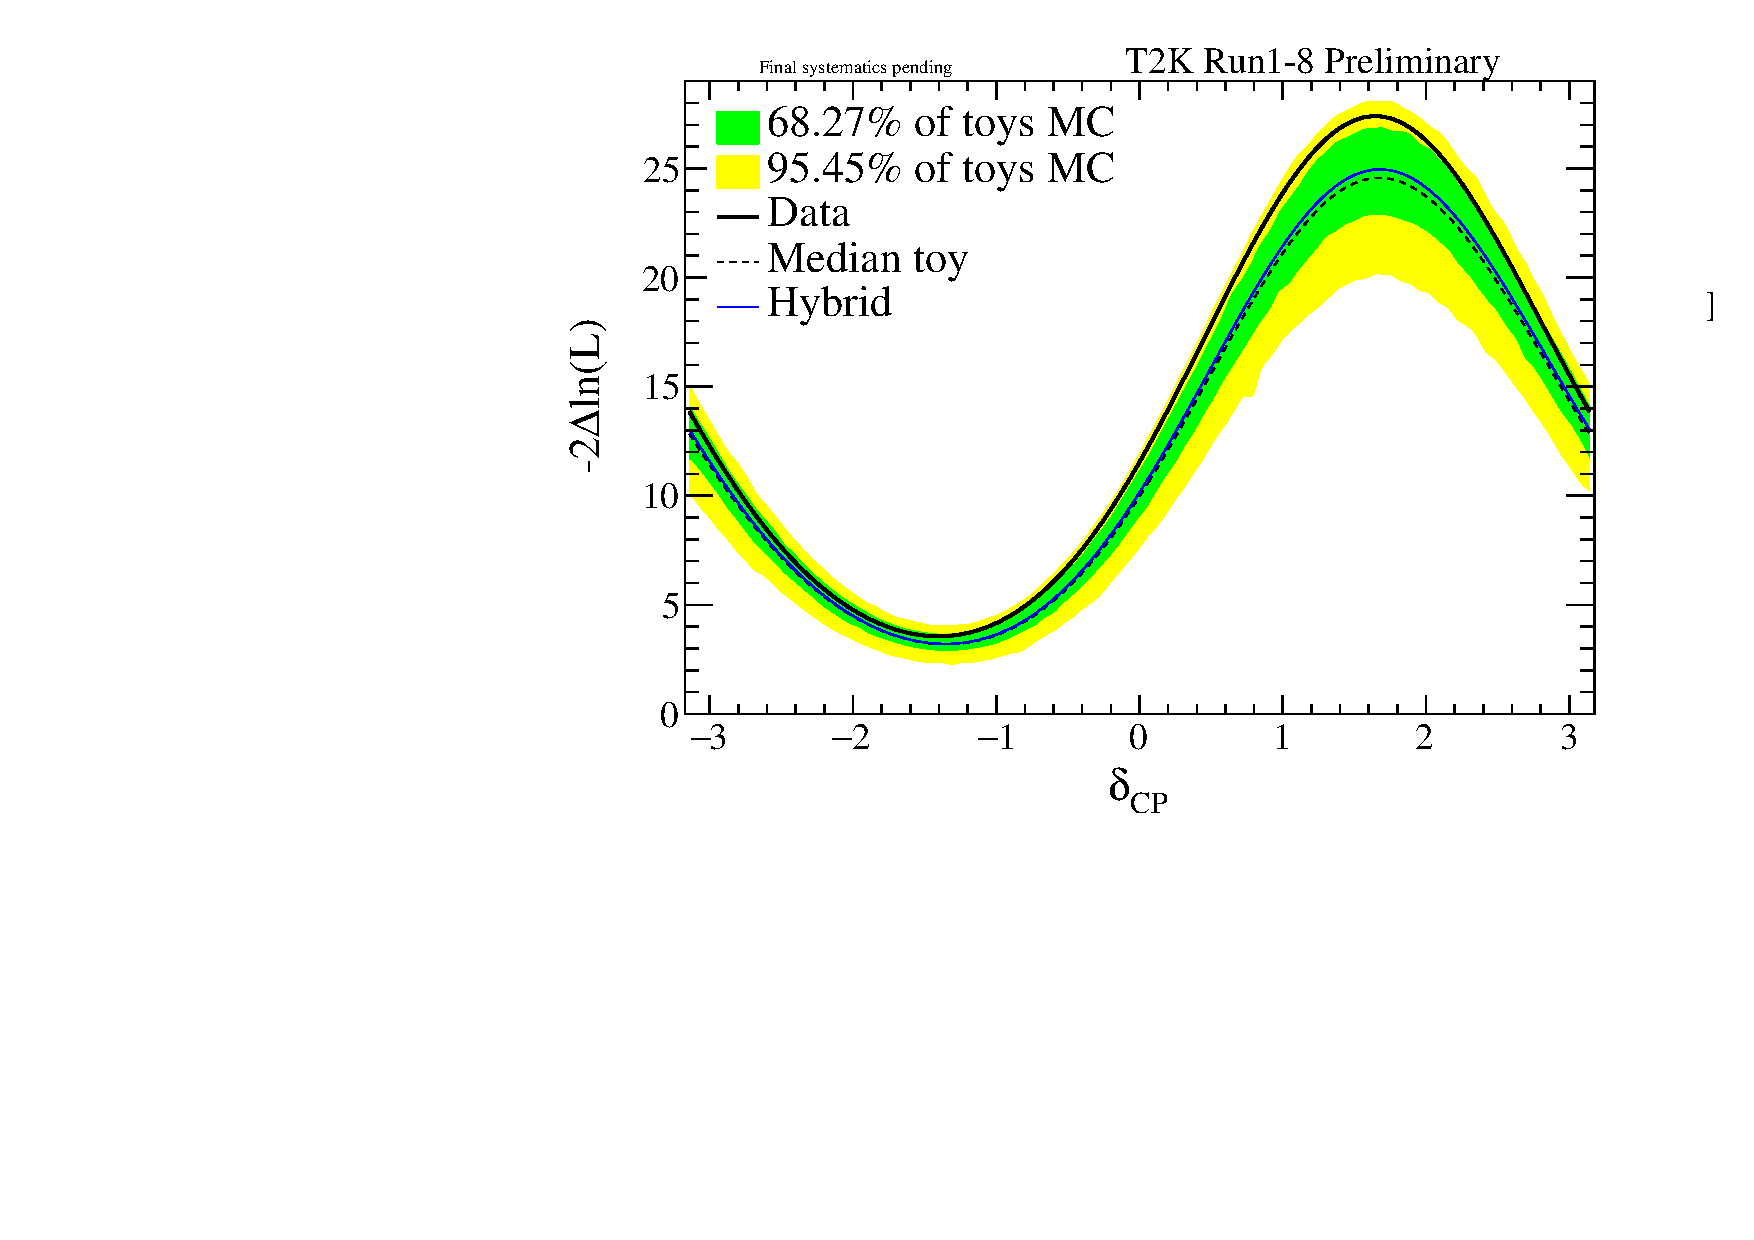
\includegraphics[width=0.9\textwidth]{comparison/deltacp_run18_fhc1rmu_braz_ih}
		\caption{Muon-like, neutrino mode}
	\end{subfigure}
	\begin{subfigure}[b]{0.49\textwidth}
		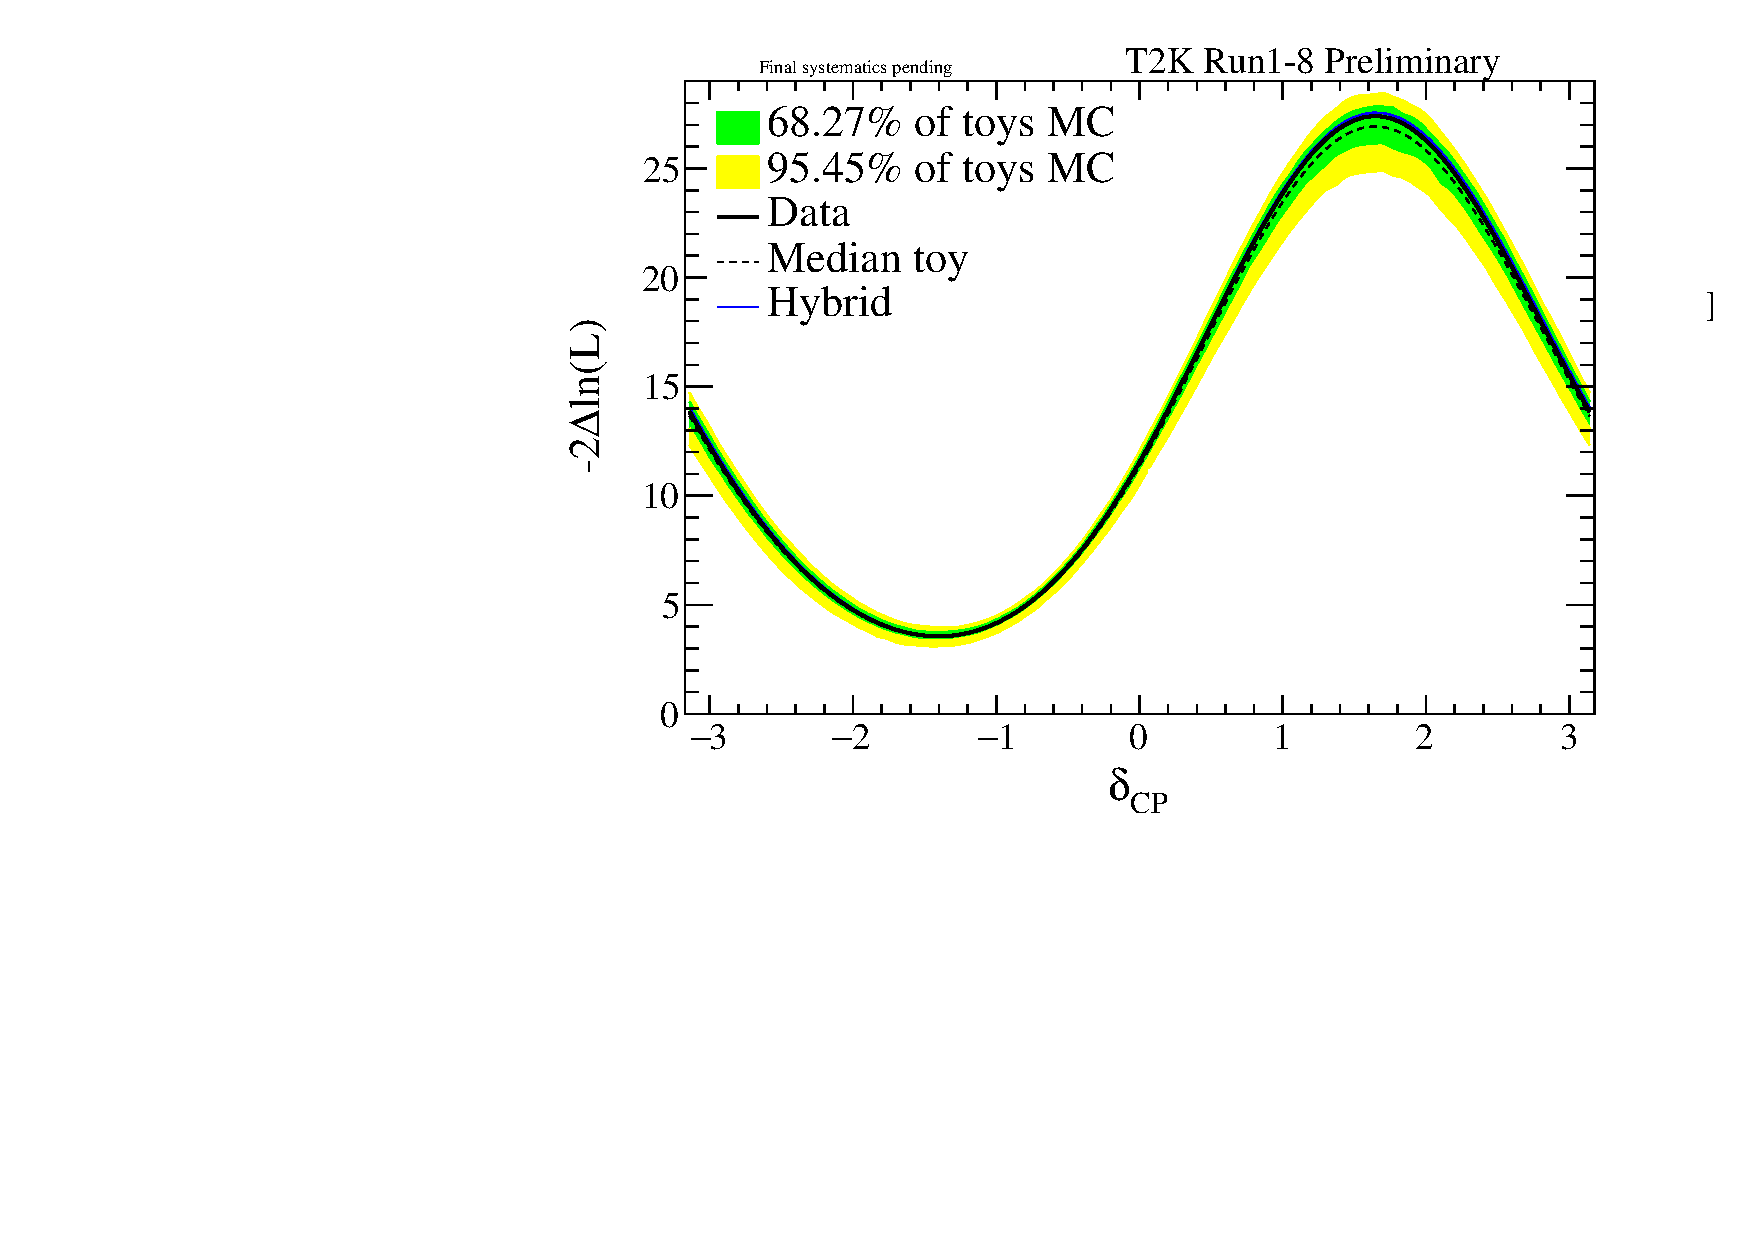
\includegraphics[width=0.9\textwidth]{comparison/deltacp_run18_rhc1rmu_braz_ih}
		\caption{Muon-like, antineutrino mode}
	\end{subfigure}
	\begin{subfigure}[b]{0.49\textwidth}
		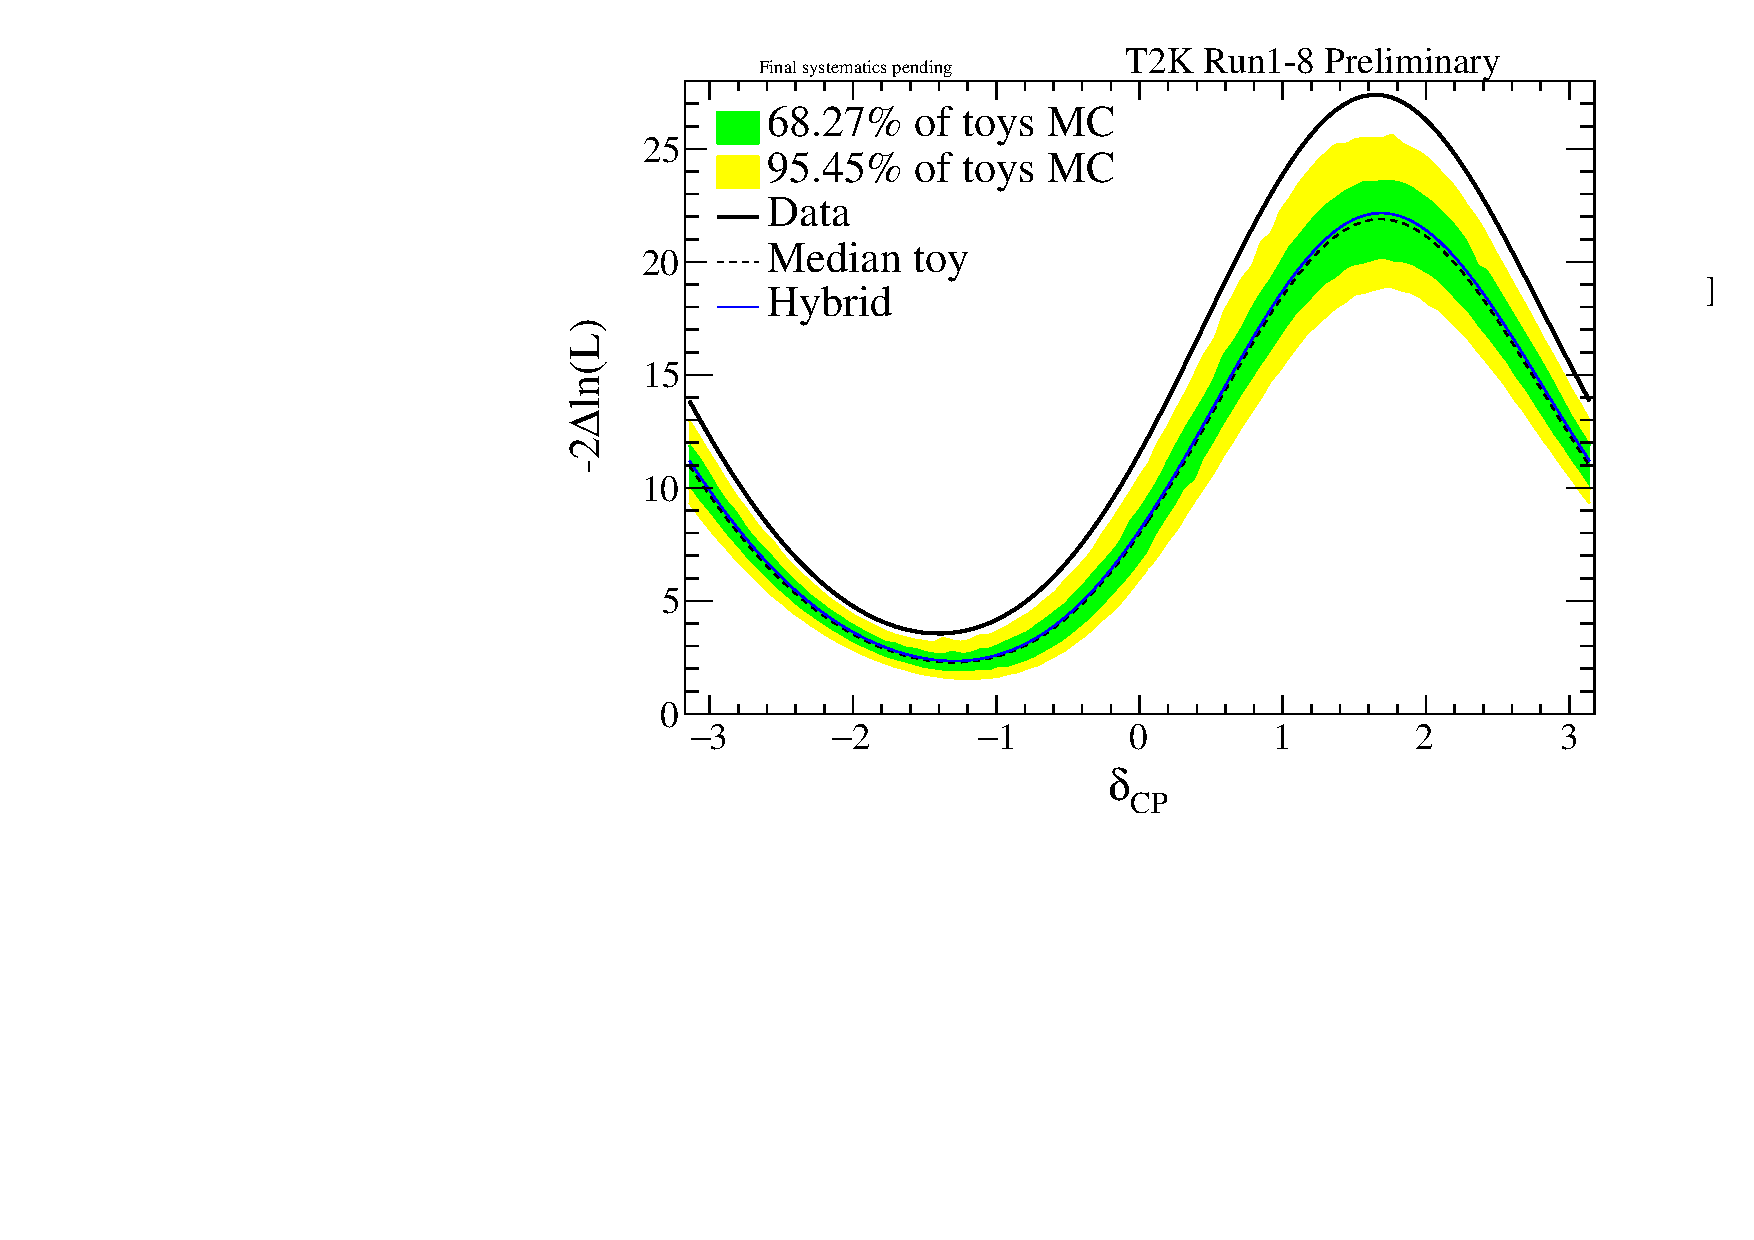
\includegraphics[width=0.9\textwidth]{comparison/deltacp_run18_cc1pi_braz_ih}
		\caption{\nueCConepi-like, neutrino mode}
	\end{subfigure}
	\caption {
		The distribution of $\Delta\chi^2$ vs \deltacp obtained with \num{1e4} toy experiments generated with $\delta_{CP} = -1.833$ and normal hierarchy is shown. The $\Delta\chi^2$ distribution obtained from the full 5-sample fit, obtained by fixing the mass hierarchy to inverted, is shown, along with the $\Delta\chi^2$ values corresponding to 68.27\% and 95.45\% of the toy experiments for the indicated sample, with all other samples fixed at their observed spectra.
	}
	\label{fig:brazilian_dcp_ih_samples}
\end{figure*}

It can be seen from \cref{fig:brazilian_dcp_nh_samples} that for normal hierarchy the observed contour resides within the $1\sigma$ band of expected sensitivities for 4 of the samples and thus while three of these contours are contributing to a stronger constraint than expected, the additional strength of the constraint in these samples is by no means surprising.

The contribution from the \nueCConepi sample is rather extreme, as might be expected given the excess events observed in this sample, with the observed contour falling outside the $2\sigma$ band of expected sensitivities for this sample. Nonetheless, with all 5 samples considered together, as in \cref{fig:brazilian_dcp_mpi2}(a), the observed constraint resides approximately within the $2\sigma$ expected sensitivity.

For the case of inverted hierarchy (\cref{fig:brazilian_dcp_ih_samples}) a similar scenario is observed, the principal difference being that the FHC one-ring $\mu$-like sample has an observed contour contained with the $2\sigma$ band of expected sensitivities, though the full 5 sample contour remains within the $2\sigma$ expected sensitivity (\cref{fig:brazilian_dcp_mpi2}).

\subsection {Comparison of \ssqthtwothree versus mass hierarchy result with sensitivity}
\label{sec:results:brazilian_mixing23}

This section provides a comparison of the \RunPeriod data fit with the expected sensitivity for \ssqthtwothree.

The procedure used is the one outline in \cref{sec:results:brazilian:method} for the two-sided distribution, with the appropriate change in oscillation parameter. Furthermore, whereas the expected sensitivity method for \deltacp throws the atmospheric parameters from a 2D likelihood distribution from on an Asimov fake data set, whose oscillation parameter values are those from the disappearance data fit, in this case the \dmsqtwothree parameter is thrown from the 1D projection of this likelihood distribution.

\subsubsection{$\sin^2\theta_{23} = 0.530$ - normal hierarchy}

In \cref{fig:brazilian_mixing23_bestfit} the \RunPeriod data result for \ssqthtwothree versus mass hierarchy is compared to the $1\sigma$ and $2\sigma$ uncertainties on the $\Delta\chi^2$ distributions corresponding to $\sin^2\theta_{23} = 0.530$ for (a) normal hierarchy and (b) inverted hierarchy.

\begin{figure*}[htb]
	\center
	\begin{subfigure}[b]{0.49\textwidth}
		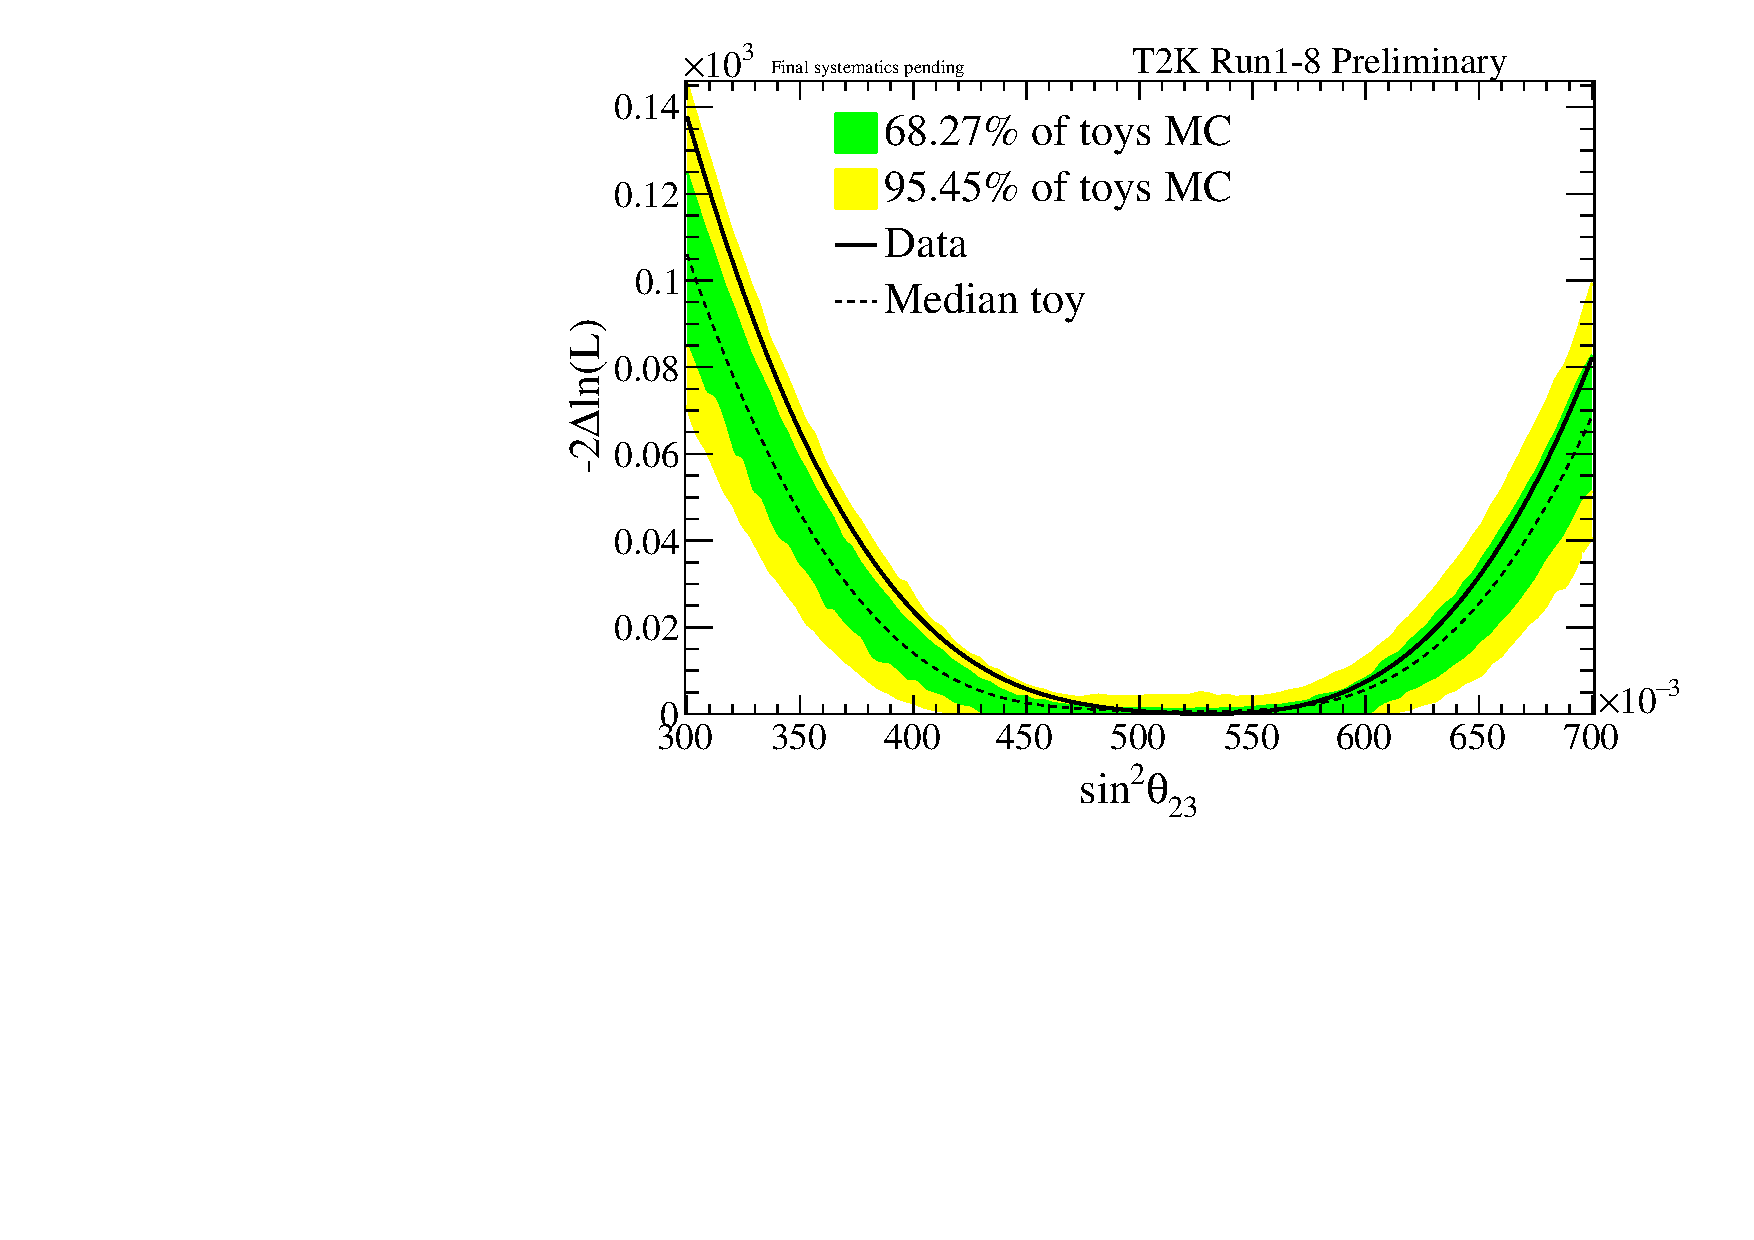
\includegraphics[width=0.9\textwidth]{comparison/mixing23/mixing23_run18_all_twosided_braz_nh}
		\caption{Normal hierarchy}
	\end{subfigure}
	\begin{subfigure}[b]{0.49\textwidth}
		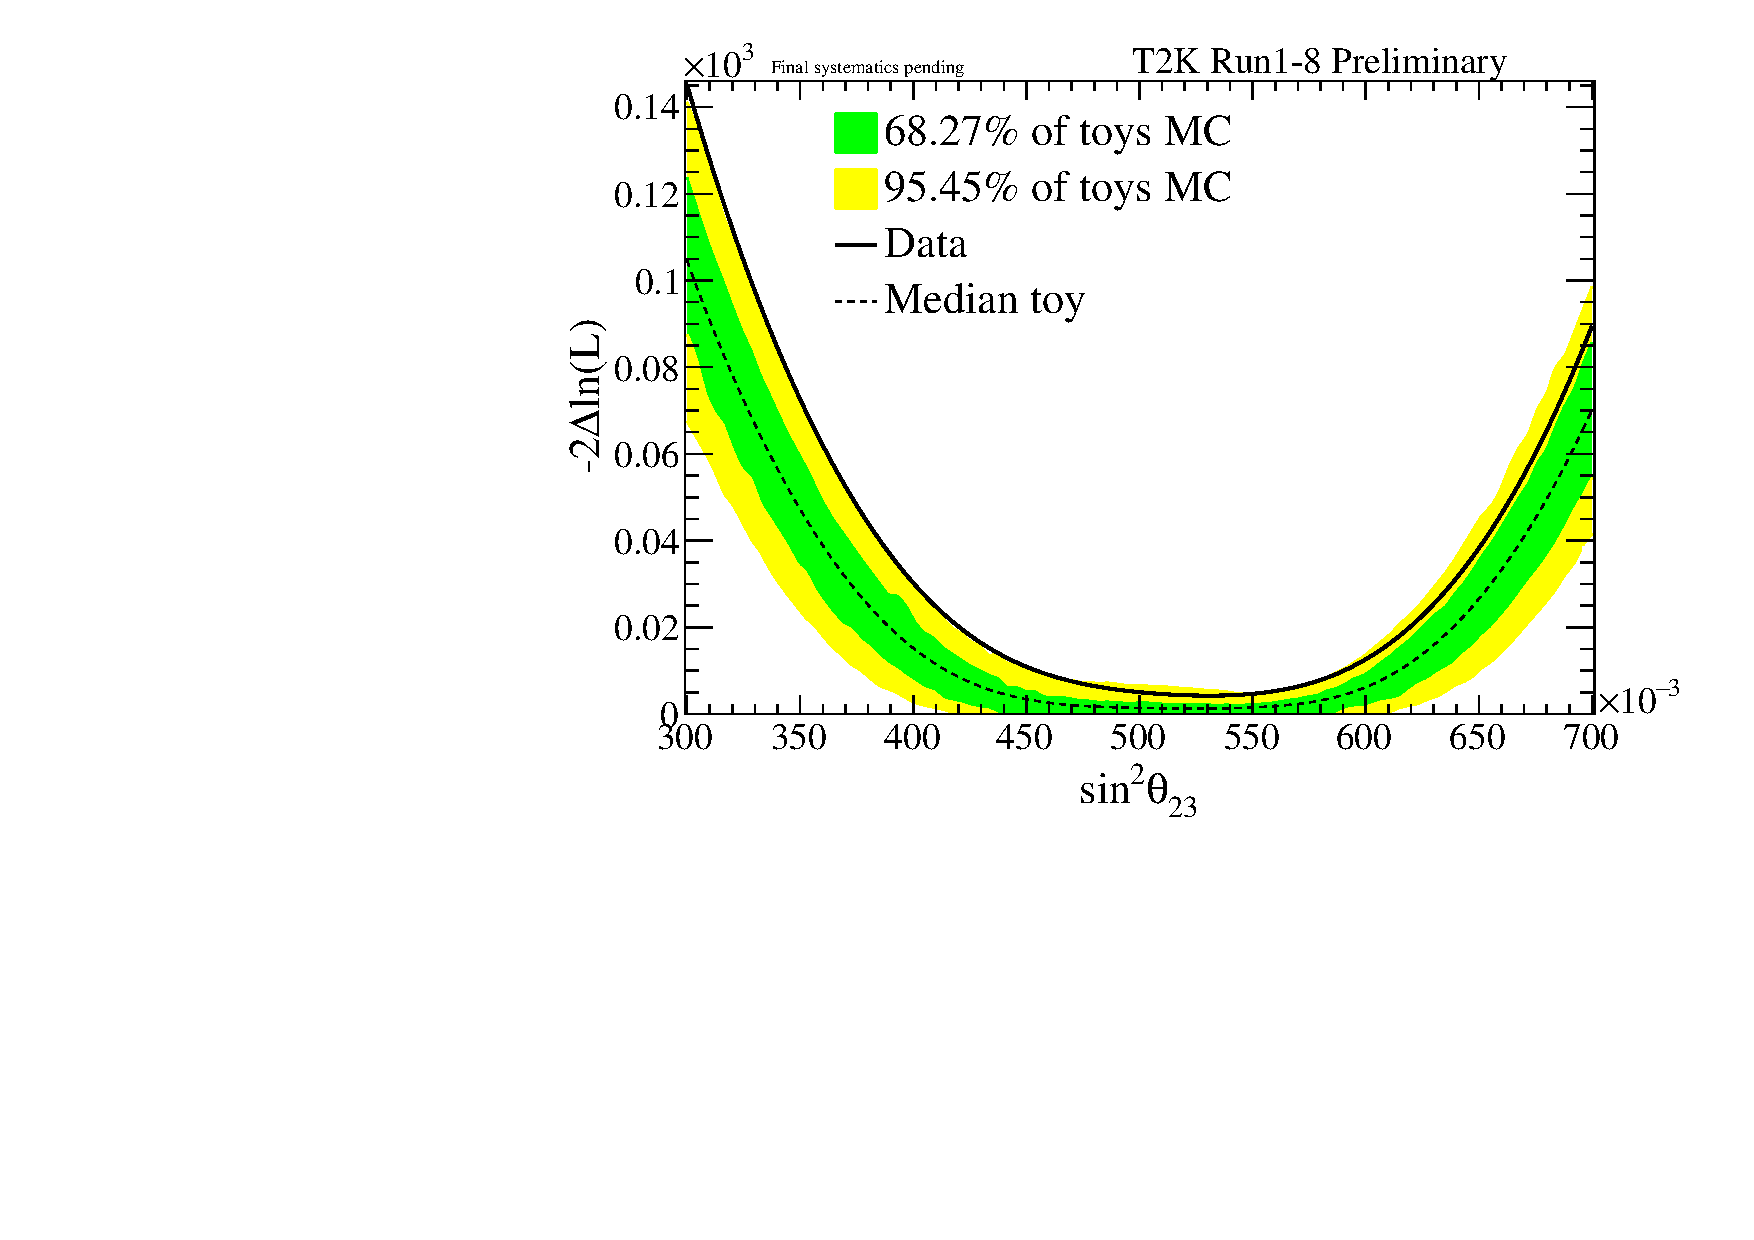
\includegraphics[width=0.9\textwidth]{comparison/mixing23/mixing23_run18_all_twosided_braz_ih}
		\caption{Inverted hierarchy}
	\end{subfigure}
	\caption {
		The distribution of $\Delta\chi^2$ vs \ssqthtwothree obtained with \num{1e4} toy experiments generated with $\sin^2\theta_{23} = 0.530$ and normal hierarchy is shown. The $\Delta\chi^2$ distributions obtained by fixing the mass hierarchy to normal (left) and inverted (right) are shown, along with the $\Delta\chi^2$ values corresponding to 68.27\% and 95.45\% of the toy experiments, the median toy and the data contour.
	}
	\label{fig:brazilian_mixing23_bestfit}
\end{figure*}

\subsection {Comparison of \dmsqtwothree versus mass hierarchy result with sensitivity}
\label{sec:results:brazilian_dmsq}

This section provides a comparison of the \RunPeriod data fit with the expected sensitivity for \dmsqtwothree.

The procedure used is the one outline in \cref{sec:results:brazilian:method} for the two-sided distribution, with the appropriate change in oscillation parameter. Furthermore, whereas the expected sensitivity method for \deltacp throws the atmospheric parameters from a 2D likelihood distribution from on an Asimov fake data set, whose oscillation parameter values are those from the disappearance data fit, in this case the \ssqthtwothree parameter is thrown from the 1D projection of this likelihood distribution.

\subsubsection{$\Delta m^2_{32} = -2.462 \times 10^{-3} \text{eV}^2\text{ c}^{-4}$ - normal hierarchy}

In \cref{fig:brazilian_dmsq23_bestfit} the \RunPeriod data result for \dmsqtwothree versus mass hierarchy is compared to the $1\sigma$ and $2\sigma$ uncertainties on the $\Delta\chi^2$ distributions corresponding to $\Delta m^2_{32} = -2.462 \times 10^{-3} \text{eV}^2\text{ c}^{-4}$ for (a) normal hierarchy and (b) inverted hierarchy.

\begin{figure*}[htb]
	\center
	\begin{subfigure}[b]{0.49\textwidth}
		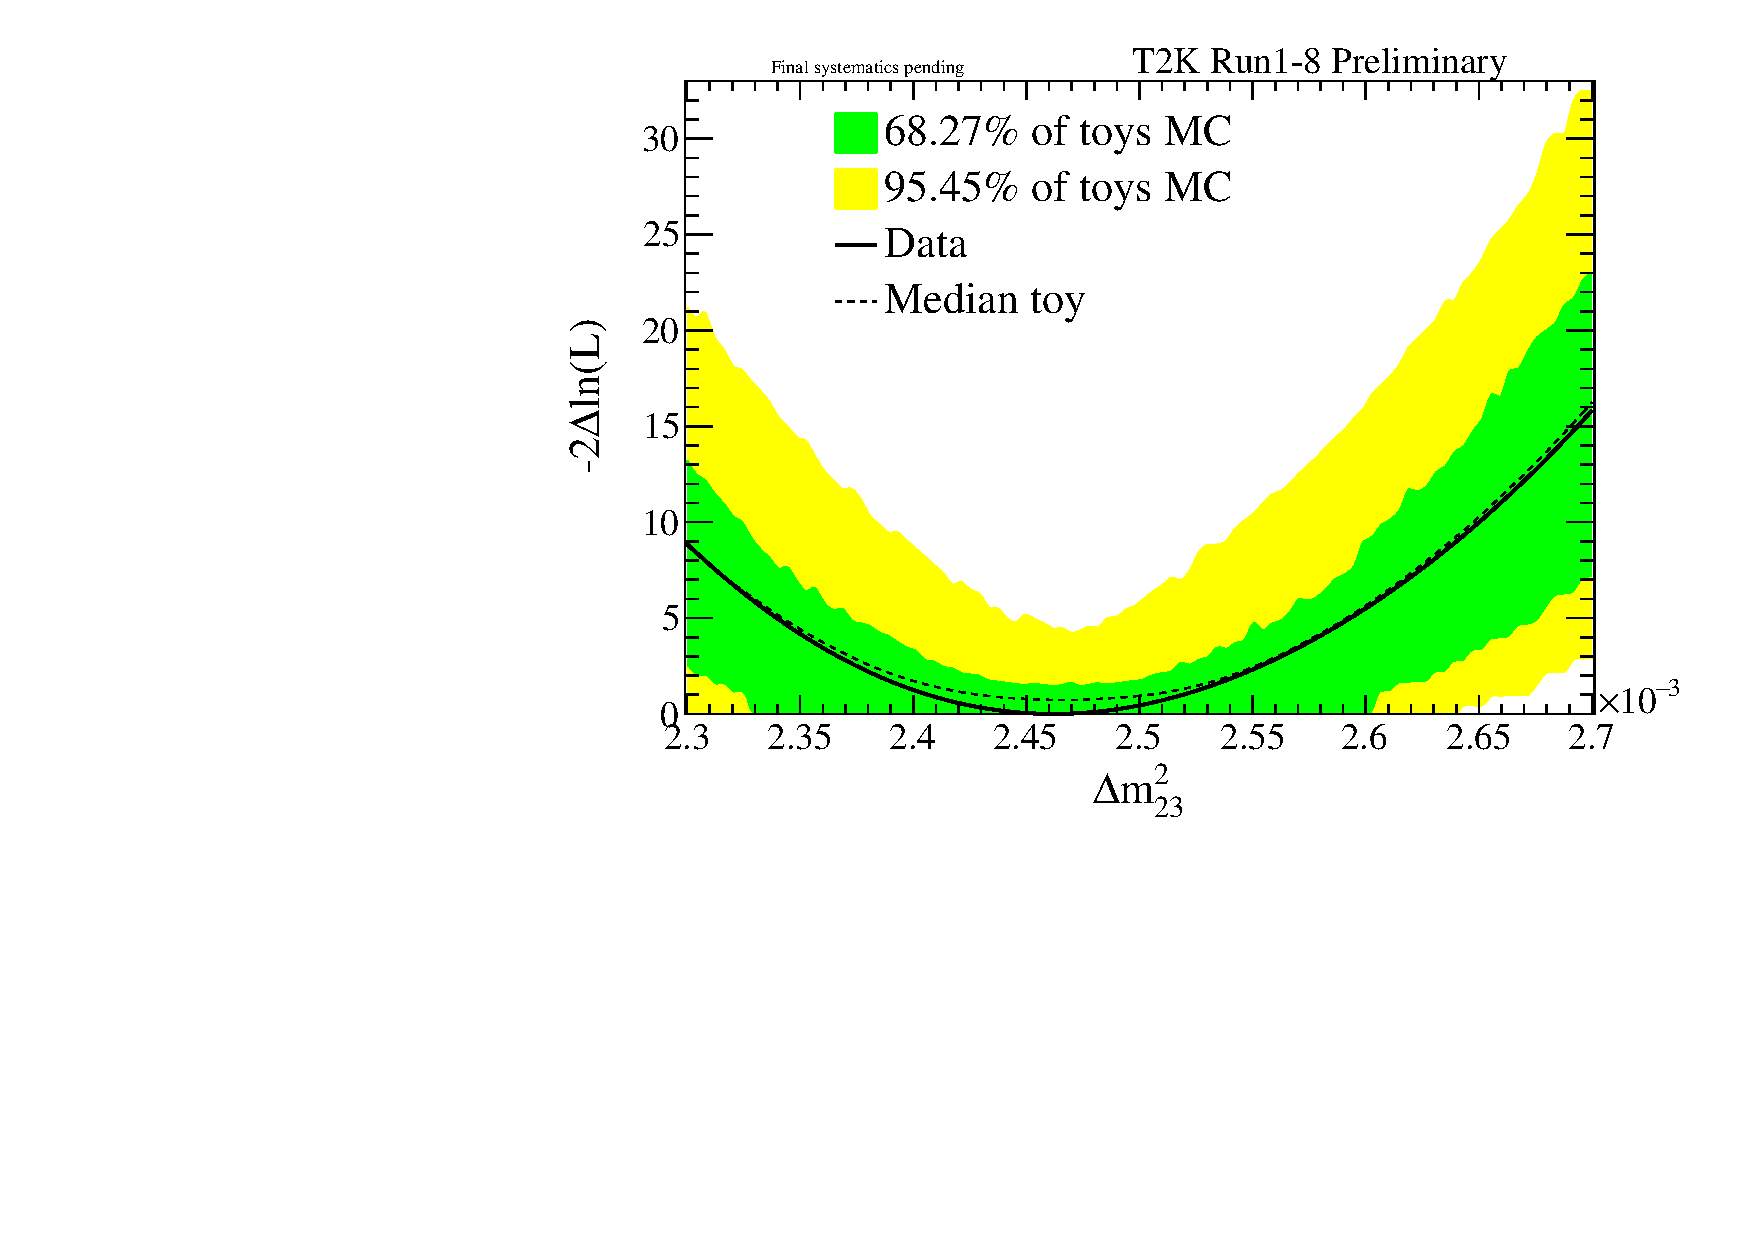
\includegraphics[width=0.9\textwidth]{comparison/dmsq23/dmsq23_run18_all_twosided_braz_nh}
		\caption{Normal hierarchy}
	\end{subfigure}
	\begin{subfigure}[b]{0.49\textwidth}
		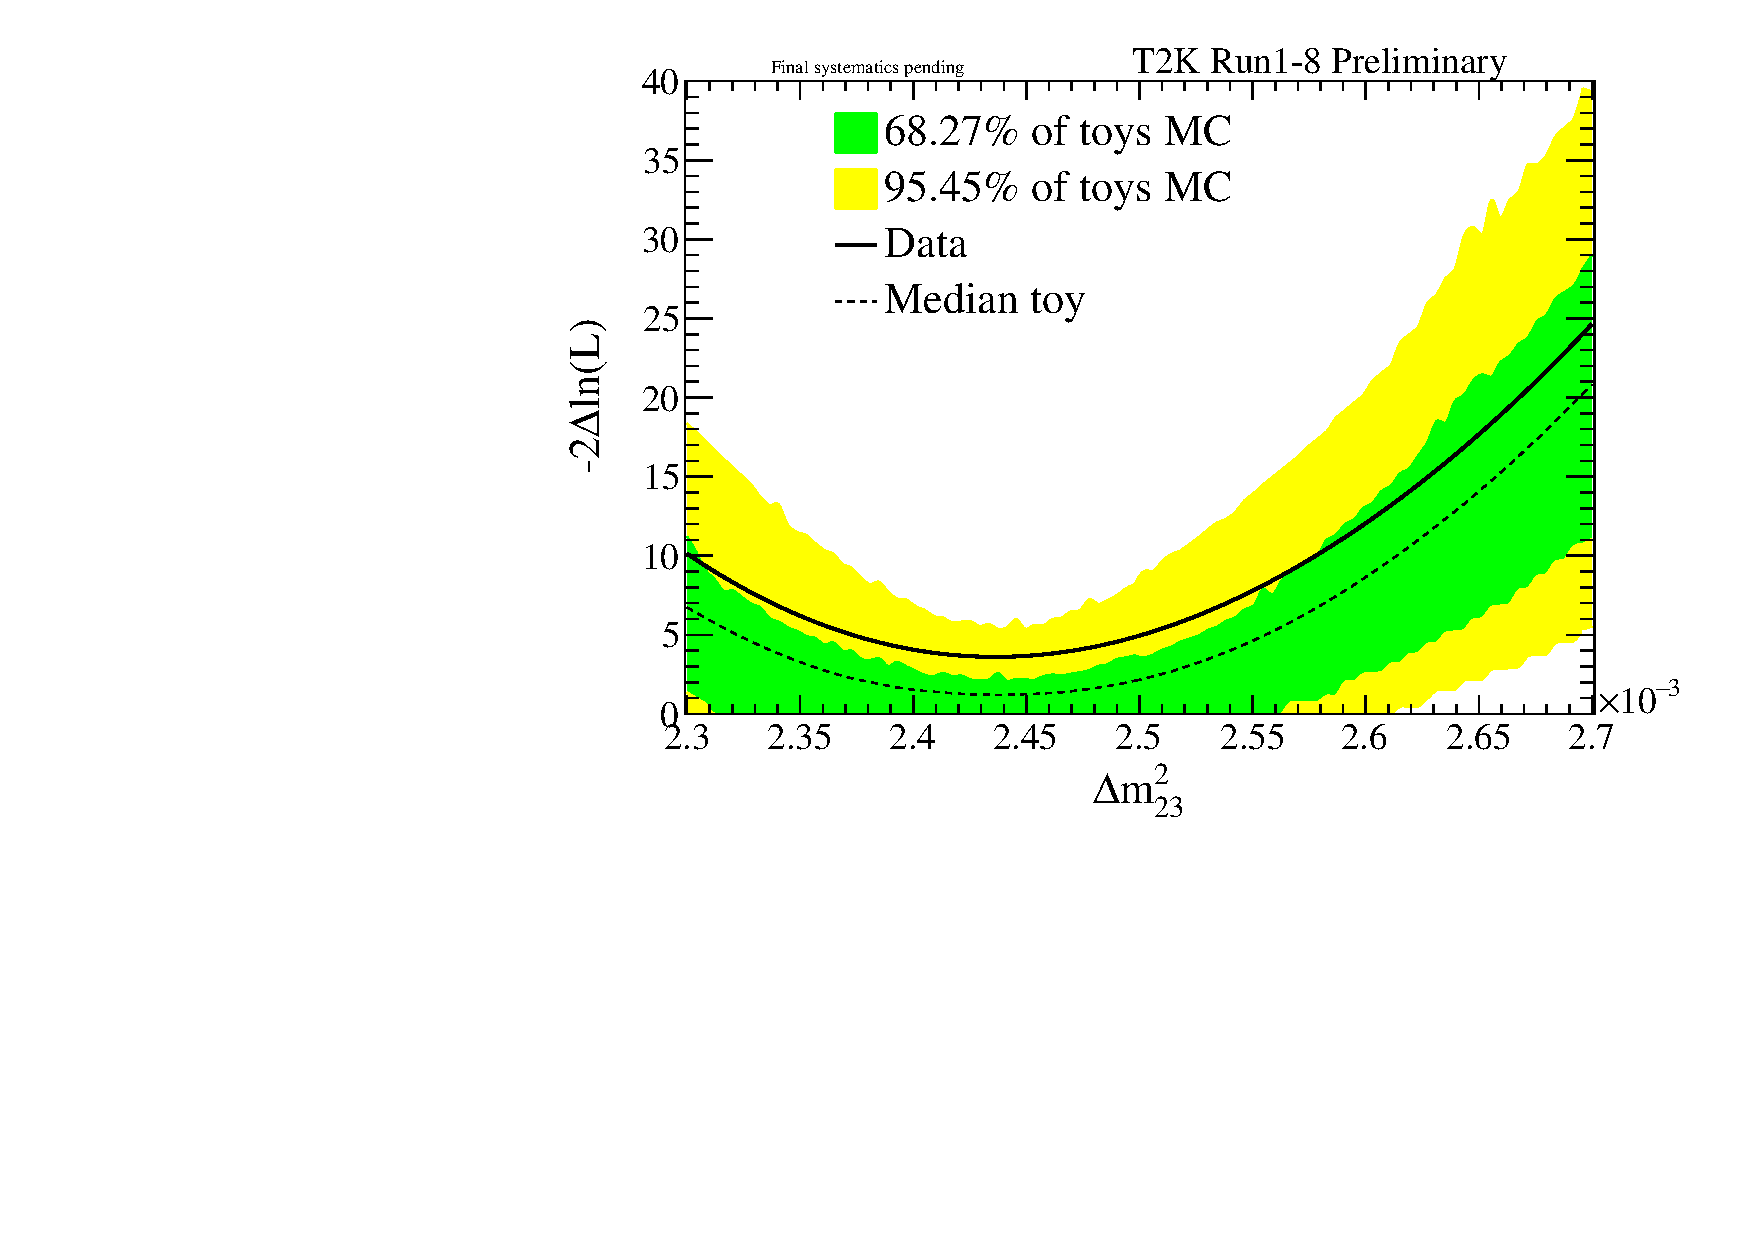
\includegraphics[width=0.9\textwidth]{comparison/dmsq23/dmsq23_run18_all_twosided_braz_ih}
		\caption{Inverted hierarchy}
	\end{subfigure}
	\caption {
		The distribution of $\Delta\chi^2$ vs \dmsqtwothree obtained with \num{1e4} toy experiments generated with $\Delta m^2_{32} = -2.462 \times 10^{-3} \text{eV}^2\text{ c}^{-4}$ and normal hierarchy is shown. The $\Delta\chi^2$ distributions obtained by fixing the mass hierarchy to normal (left) and inverted (right) are shown, along with the $\Delta\chi^2$ values corresponding to 68.27\% and 95.45\% of the toy experiments, the median toy and the data contour.
	}
	\label{fig:brazilian_dmsq23_bestfit}
\end{figure*}

\subsection {Comparison of $e$-like event rates with expectation}
\label{sec:results:bievent}
It is valuable to see how different values of \deltacp, \ssqthtwothree and hierarchy affect the predicted event rates. \Cref{fig:bievent} shows the predicted $\nueb$ event rate vs $\nue$ event rate for best-fit values of oscillation parameters where \deltacp is varied between CP conserving and maximally CP violating values, and \ssqthtwothree is varied around its best-fit, for both hierarchies. Event rates for a given value of \ssqthtwothree and mass hierarchy are linearly interpolated between those computed for 9 evenly-spaced values of \deltacp from $-\pi$ to $+\pi$ to indicate the behaviour produced by varying \deltacp. The observed event rates with $1\sigma$ errors are also shown. \Cref{fig:bievent}(a) shows $e$-like event rates where the FHC sample includes the \nueCConepi sample, while \cref{fig:bievent}(b) shows $e$-like event rates where the FHC sample does not include the \nueCConepi sample.
\begin{figure*}[htb]
	\center
	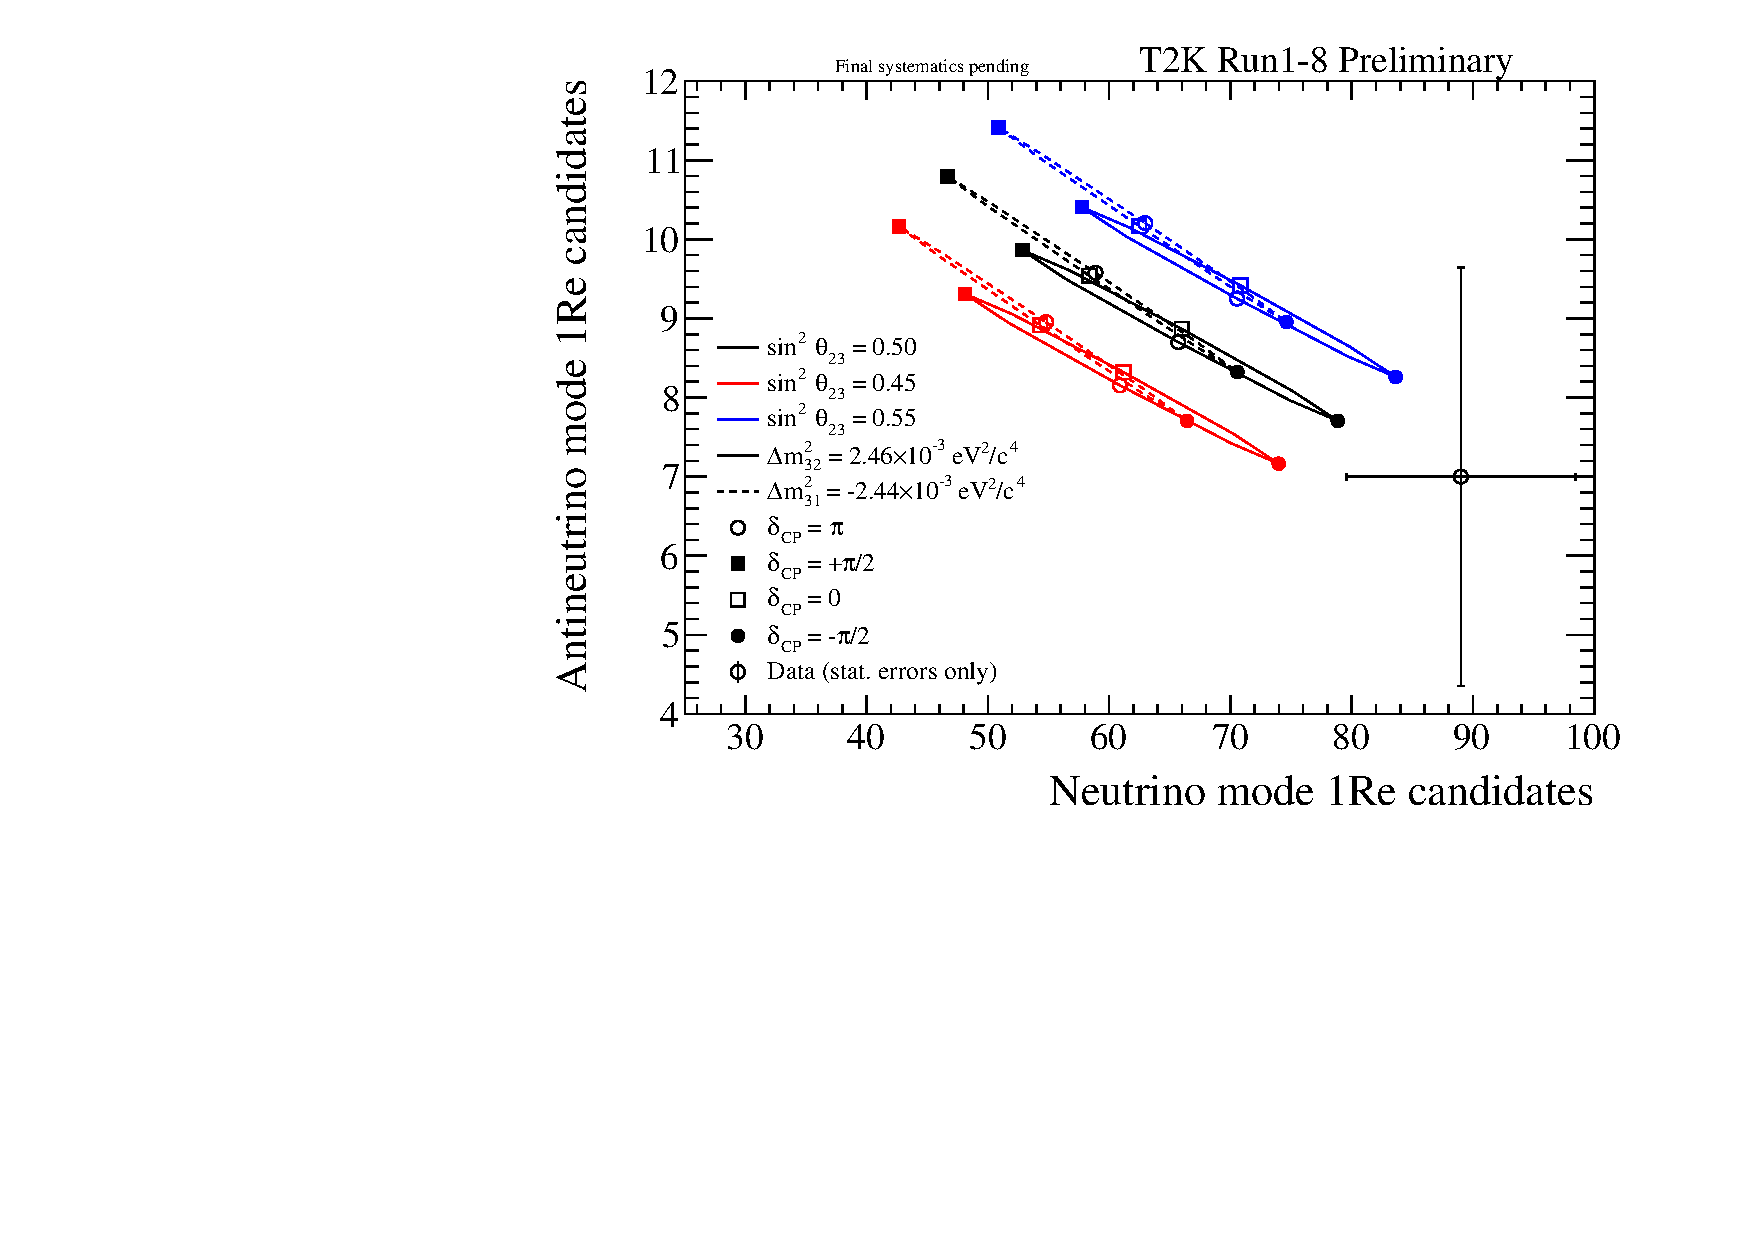
\includegraphics[width=0.7\textwidth]{studies/bievent/ellipse_cc1pi_all}
	\caption {
		This plot shows the candidate RHC one-ring $e$-like event rate vs the candidate FHC one-ring $e$-like event rate for a variety of different oscillation parameter values. Predictions are generated for best-fit values of oscillation parameters for different values of \deltacp, \ssqthtwothree and mass hierarchy. In particular the FHC and RHC event rates are plotted for the CP conserving and maximally CP violating values of \deltacp, with \ssqthtwothree set at the best-fit value and $\pm 1\sigma$ values in both normal and inverted hierarchy. The observed rates with statistical error shown are also included.
	}
	\label{fig:bievent}
\end{figure*}

\clearpage

%%% Local Variables:
%%% mode: latex
%%% TeX-master: "../TN327"
%%% End:

\clearpage

\section {Updated results with $E_b$ parameter and \dmsq smearing}
\label{sec:results2017b}

\subsection{Findings from the 2017 fake data studies}

As part of the analysis procedure, a variety of fake data fits were performed to assess the robustness of the analysis to changes in the cross-section model \cite{FakeData:2017}. The conclusion of these fake data studies was that an additional source of uncertainty was necessary to address biases seen in \ssqthtwothree and \dmsq (\dmsqtwothree for normal hierarchy or \dmsqonethree for inverted hierarchy) in the $E_b$ fake data studies. Furthermore, the inclusion of the additional systematic parameter was insufficient to address the bias in \dmsq and therefore an additional smearing of the likelihood surface for this parameter was added.

\subsection{Systematic parameter update and smearing procedure}

The additional $E_b$ systematic parameter is implemented as a response function, based on weights determined by the ratio of near-to-far predicted fake data event rates and event rates seen in the fake data set. The ratio was calculated for 3 points; $-0.5\sigma$, $0\sigma$ and $+1\sigma$, with  a further 3 linearly extrapolated points at $-1.5\sigma$, $+3\sigma$ and $+5\sigma$ included to allow the response function to better conform to bi-linearity throughout the allowed $[-1.5\sigma, +5\sigma]$ range. \color{blue}Negative weights that can result from the extrapolation are set to zero.\color{black}

Post-fit, the \dmsq contour is inflated via a smearing procedure. In particular, the likelihood surface resulting from the fit is scaled by a factor of 10 and resampled using Catmull-Rom cubic interpolation, before each source bin in \dmsq (for a particular value of \ssqthtwothree in the 2D fit) is smeared over the remaining \dmsq bins, with the contribution weighted by a Gaussian centred on the source bin, integrated over the target bin interval.

\subsection{Results}

The results of the \RunPeriod data set fit, for an exposure of \TotalPotNuRunOneEight POT in neutrino mode and of \TotalPotNuBarRunOneEight POT in antineutrino mode, with the $E_b$ parameter and smearing applied, are shown in this chapter.  In \cref{fig:asimovpf_spectra_mc_data_2017b} the best-fit predicted spectra of $\mu$-like and $e$-like samples are compared to the observed data. In \cref{tab:num_events_run18_2017b} the expected and observed number of events in \RunPeriod data set are shown.

\begin{table}[htb]
\centering
\begin{tabular}{| c | c | c | c |}
\hline
Beam mode & Sample & Exp. Best-fit & Observed \\
\hline
$\nu$ & $\mu$-like & 270.792 & 240 \\
$\nu$ & $e$-like & 73.099 & 74 \\
$\bar{\nu}$ & $\mu$-like & 64.997 & 68 \\
$\bar{\nu}$ & $e$-like & 7.947 & 7 \\
$\nu$ & \nueCConepi-like & 6.812 & 15 \\
\hline
\end{tabular}

\caption{
The observed and best-fit expected number of events in \RunPeriod data set for an exposure of \TotalPotNuRunOneEight POT in neutrino mode and of \TotalPotNuBarRunOneEight POT in antineutrino mode are shown 
for each selected sample. The prediction is produced using the BANFF tuning.
}
\label{tab:num_events_run18_2017b}
\end{table}

The predicted and observed spectra are shown for each of the samples in \cref{fig:asimovpf_spectra_mc_data_2017b}. The $e$-like samples are broken down into $E_\text{rec}$ and $\theta$ projections in \cref{fig:asimovpf_spectra_mc_data_elike_1D_2017b}.
\begin{figure*}[htb]
	\center
	\begin{subfigure}[b]{0.49\textwidth}
		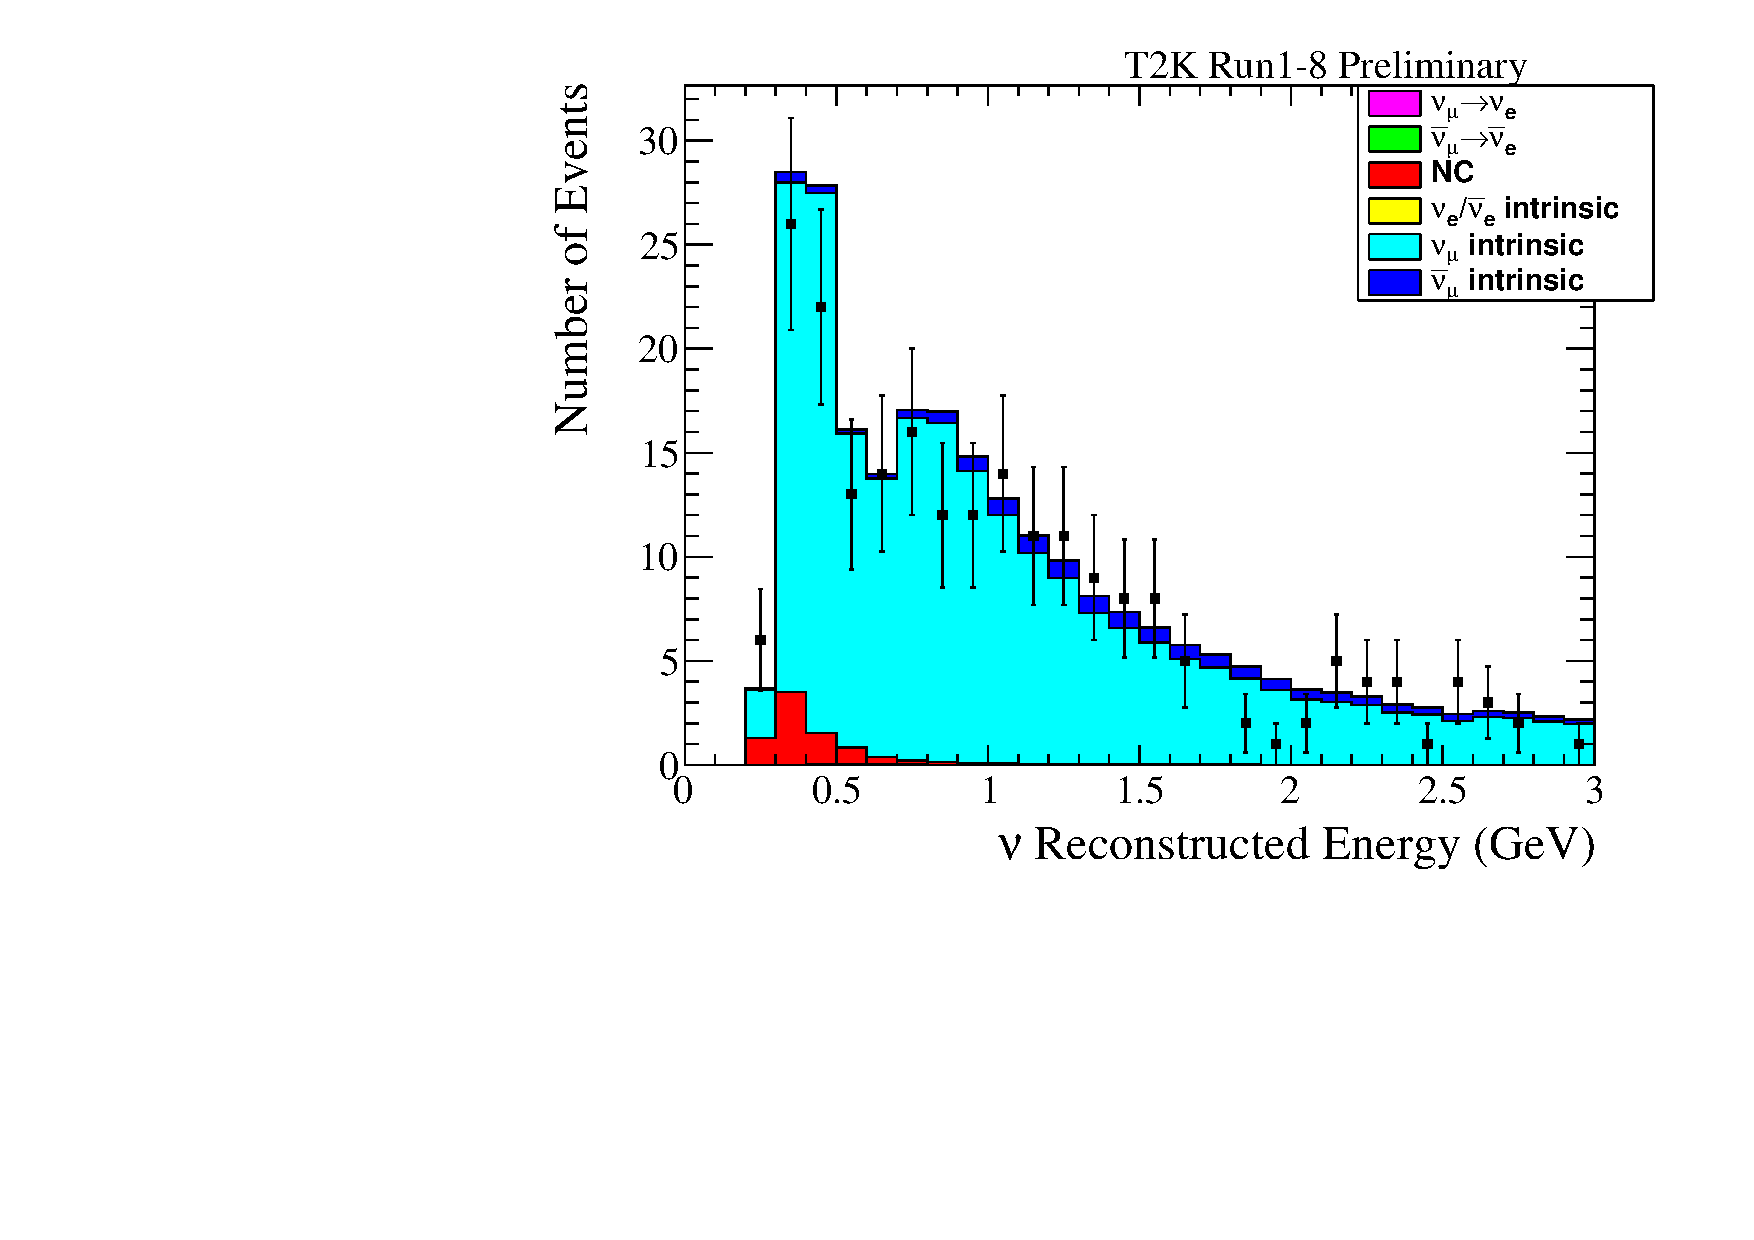
\includegraphics[width=0.9\textwidth]{spectra/2017b/spectrum_osc_asimovpf_1Rmu_data}
		\caption{Muon-like, neutrino mode}
	\end{subfigure}
	\begin{subfigure}[b]{0.49\textwidth}
		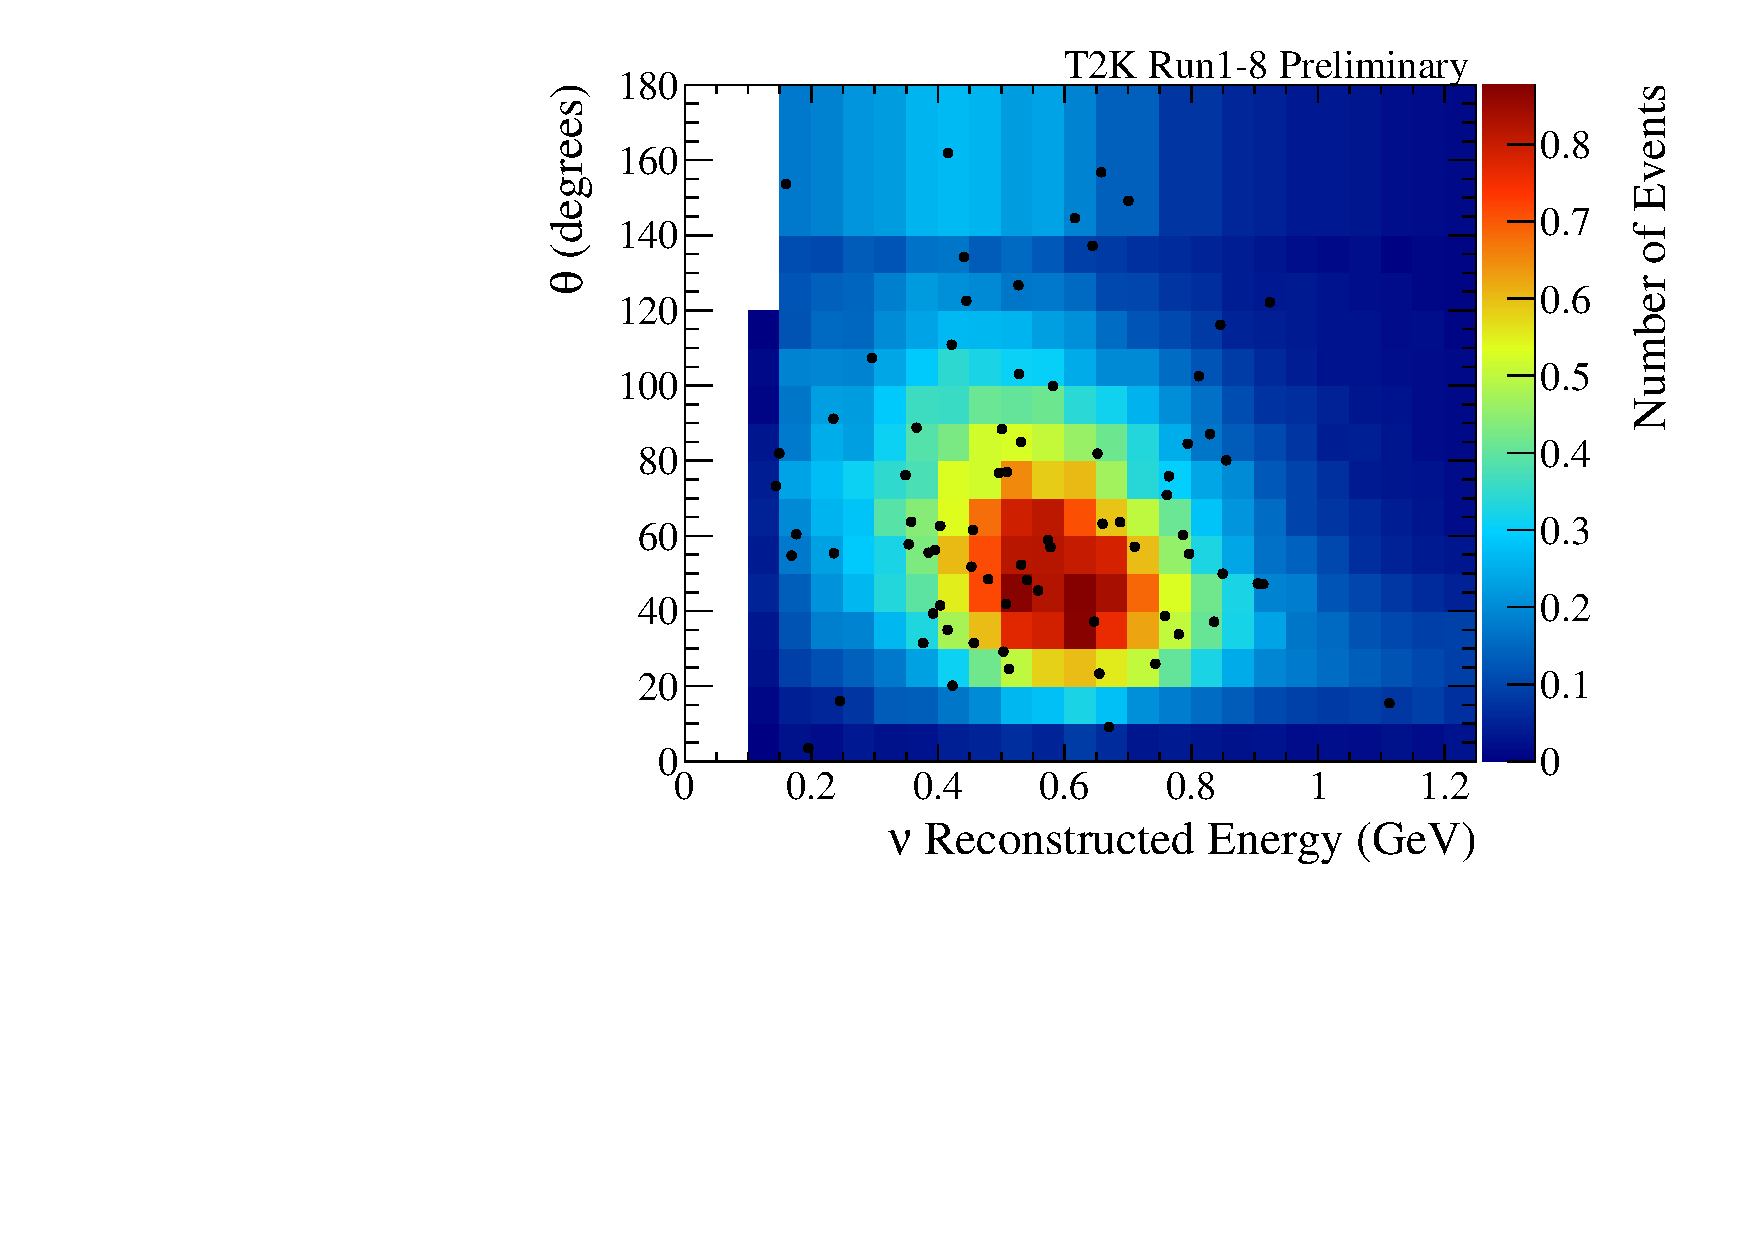
\includegraphics[width=0.9\textwidth]{spectra/2017b/spectrum_osc_asimovpf_1Re_data}
		\caption{Electron-like, neutrino mode}
	\end{subfigure}
	\begin{subfigure}[b]{0.49\textwidth}
		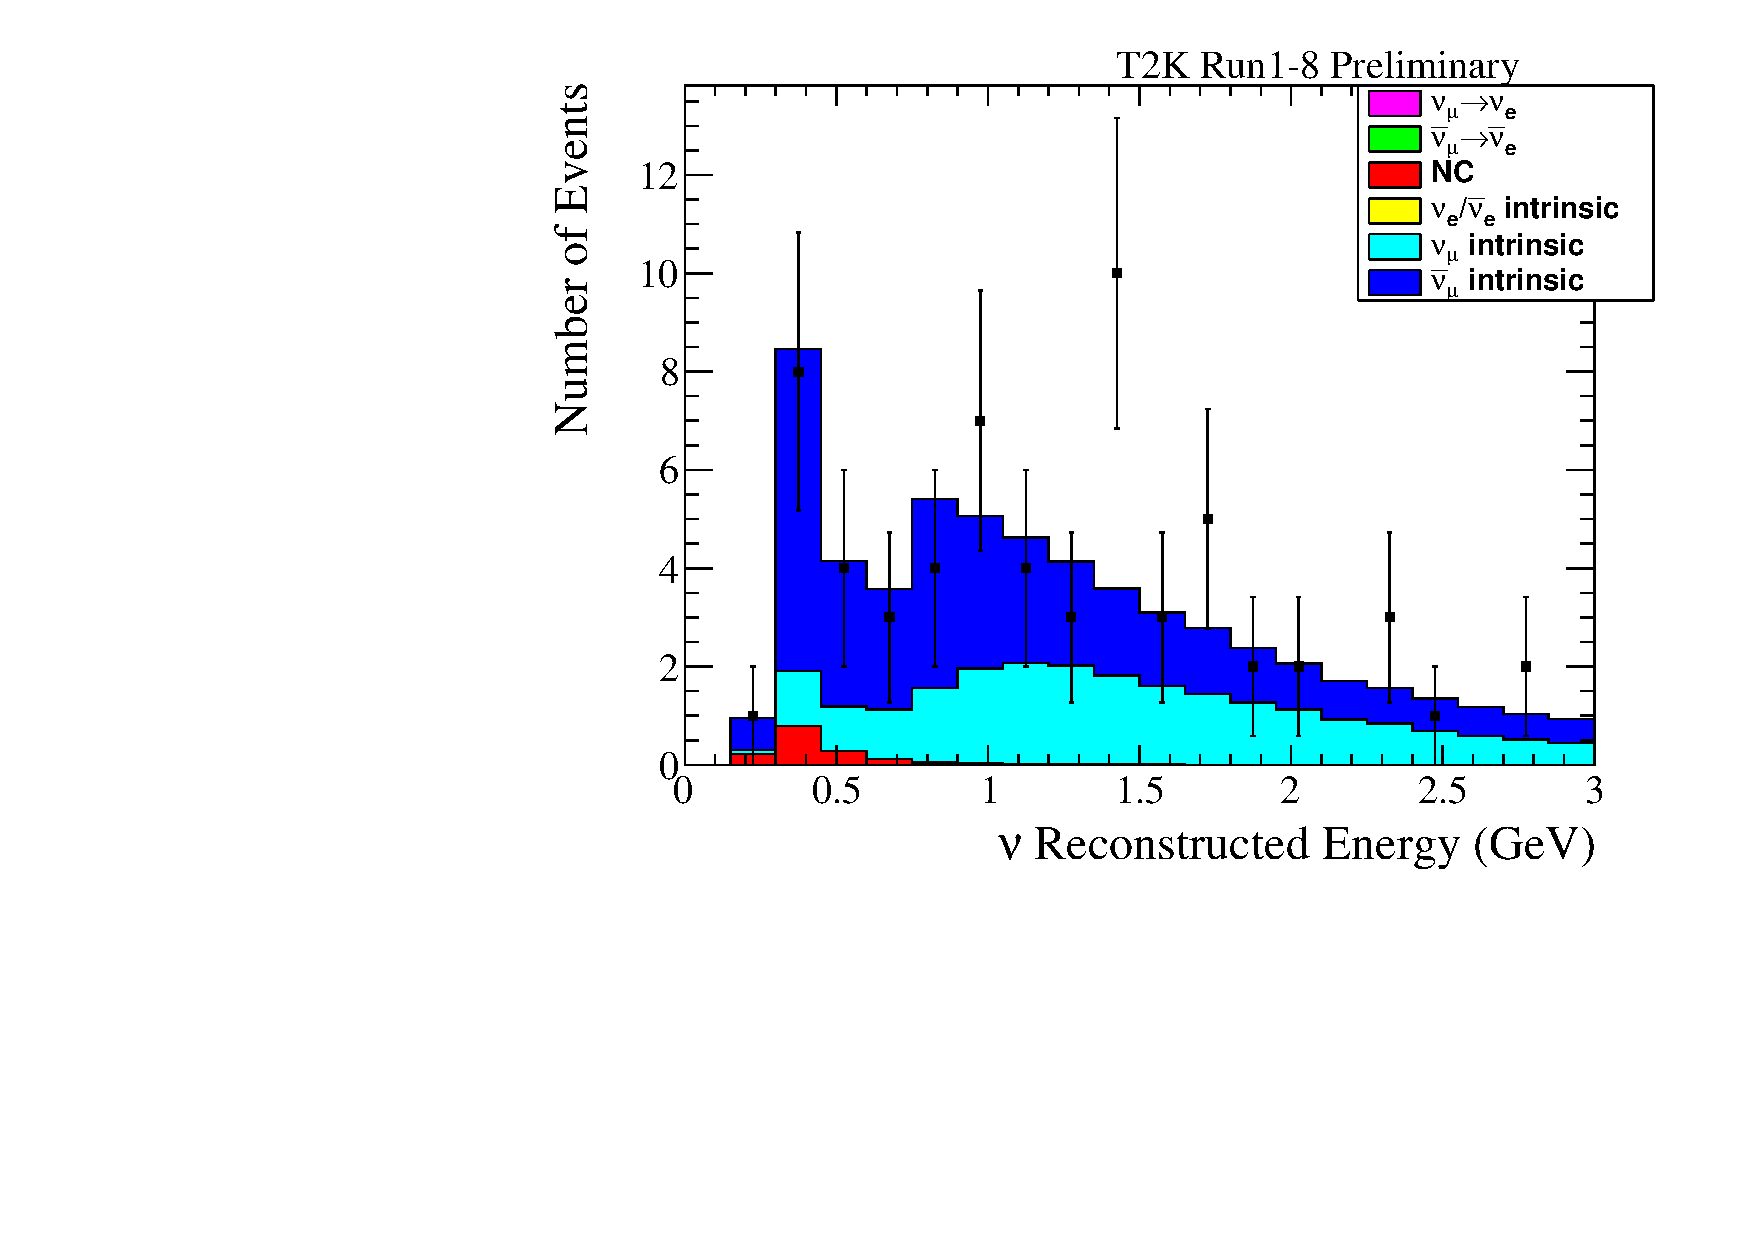
\includegraphics[width=0.9\textwidth]{spectra/2017b/spectrum_osc_asimovpf_RHC1Rmu_data}
		\caption{Muon-like, antineutrino mode}
	\end{subfigure}
	\begin{subfigure}[b]{0.49\textwidth}
		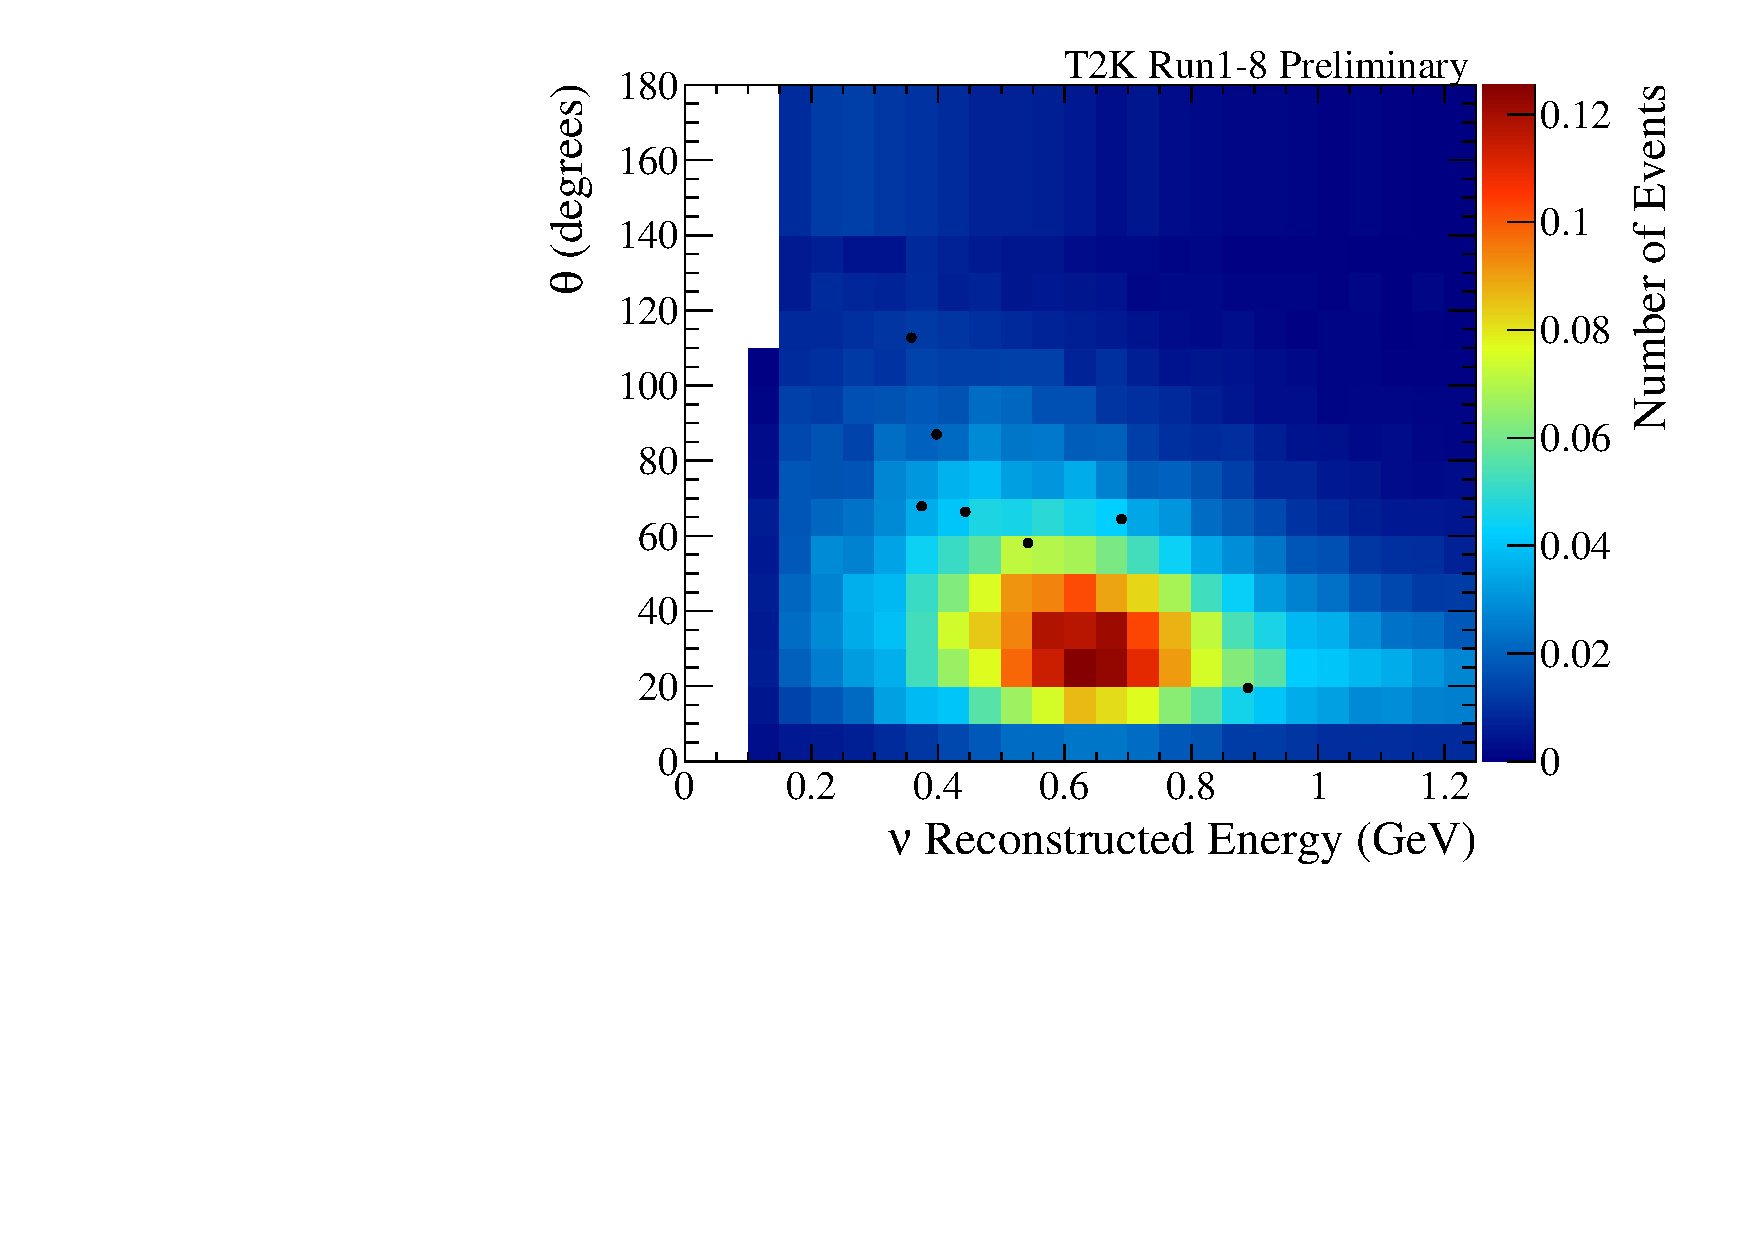
\includegraphics[width=0.9\textwidth]{spectra/2017b/spectrum_osc_asimovpf_RHC1Re_data}
		\caption{Electron-like antineutrino mode}
	\end{subfigure}
	\begin{subfigure}[b]{0.49\textwidth}
		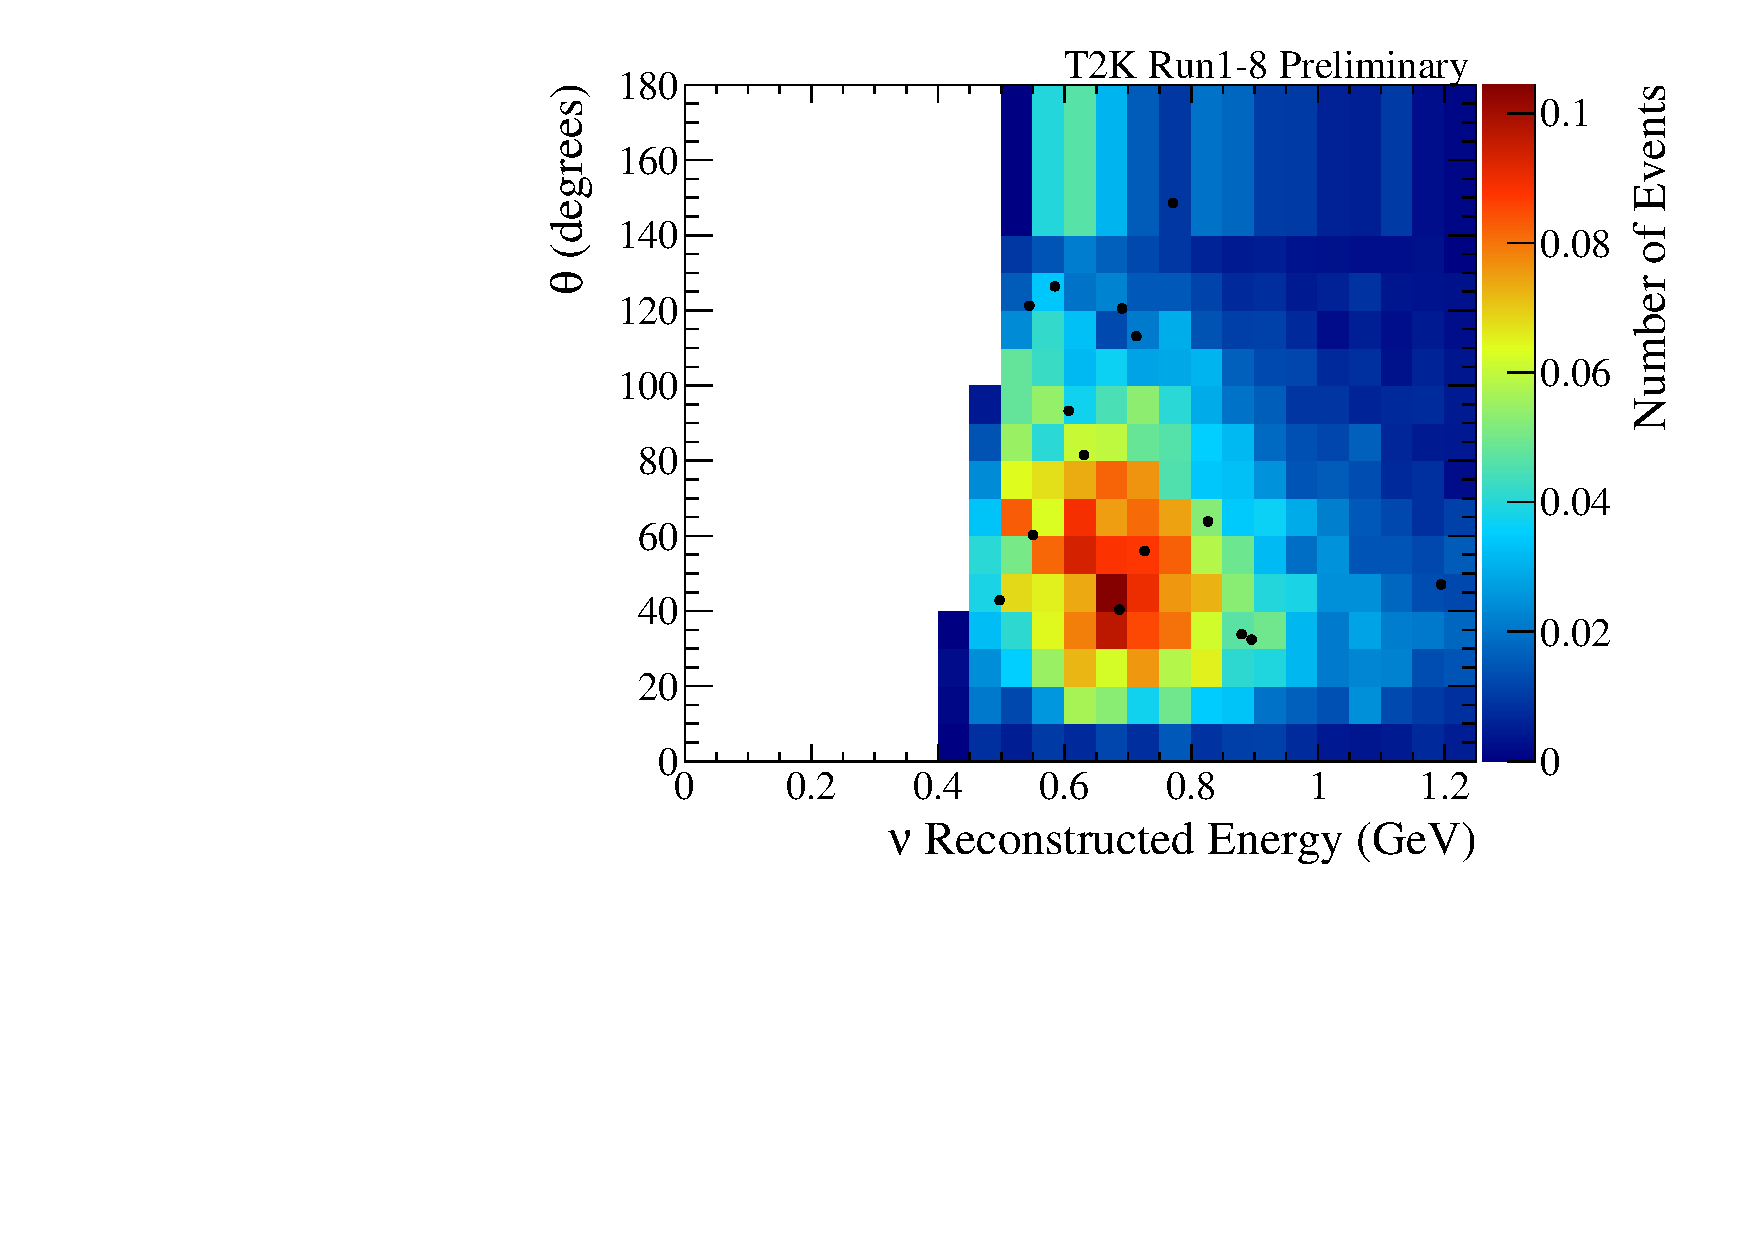
\includegraphics[width=0.9\textwidth]{spectra/2017b/spectrum_osc_asimovpf_MultiRe_data}
		\caption{\nueCConepi-like, neutrino mode}
	\end{subfigure}
	\caption {
		Predicted spectra and observed events (points). $\mu$-like distributions are a function of the reconstructed neutrino energy, while the $e$-like, including \nueCConepi, distributions are functions of both the reconstructed neutrino energy and the reconstructed angle between the outgoing lepton and the neutrino direction. The distributions correspond to the statistics collected in the full \RunPeriod data set. The spectra are generated with the systematic parameters described in \cref{sec:systematics} and the oscillation parameters corresponding to the best-fit values from the data fit (solar parameters at PDG 2016).
	}
	\label{fig:asimovpf_spectra_mc_data_2017b}
\end{figure*}
\clearpage
\begin{figure*}[htb]
	\center

	\begin{subfigure}[b]{0.49\textwidth}
		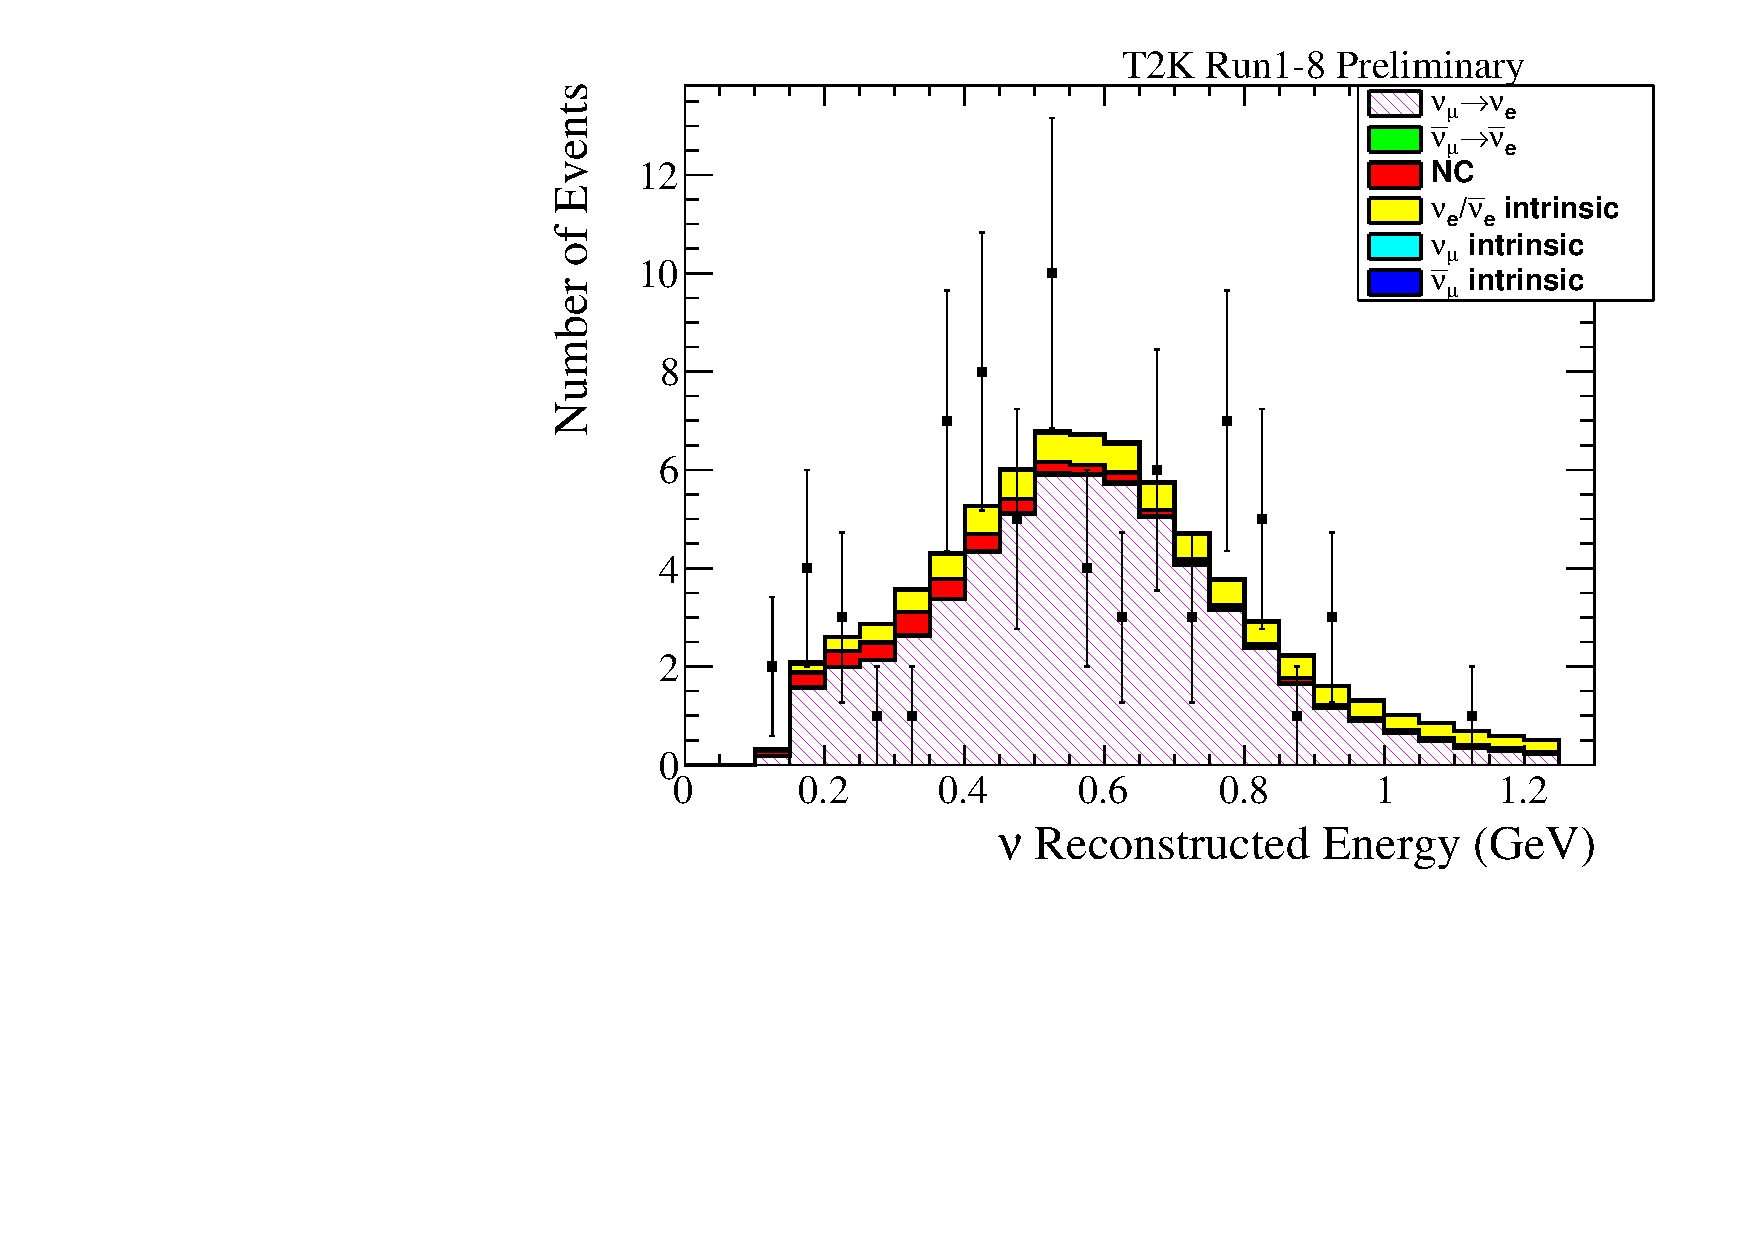
\includegraphics[width=0.9\textwidth]{spectra/2017b/erec_spectrum_osc_asimovpf_1Re_data}
		\caption{Electron-like, neutrino mode}
	\end{subfigure}
	\begin{subfigure}[b]{0.49\textwidth}
		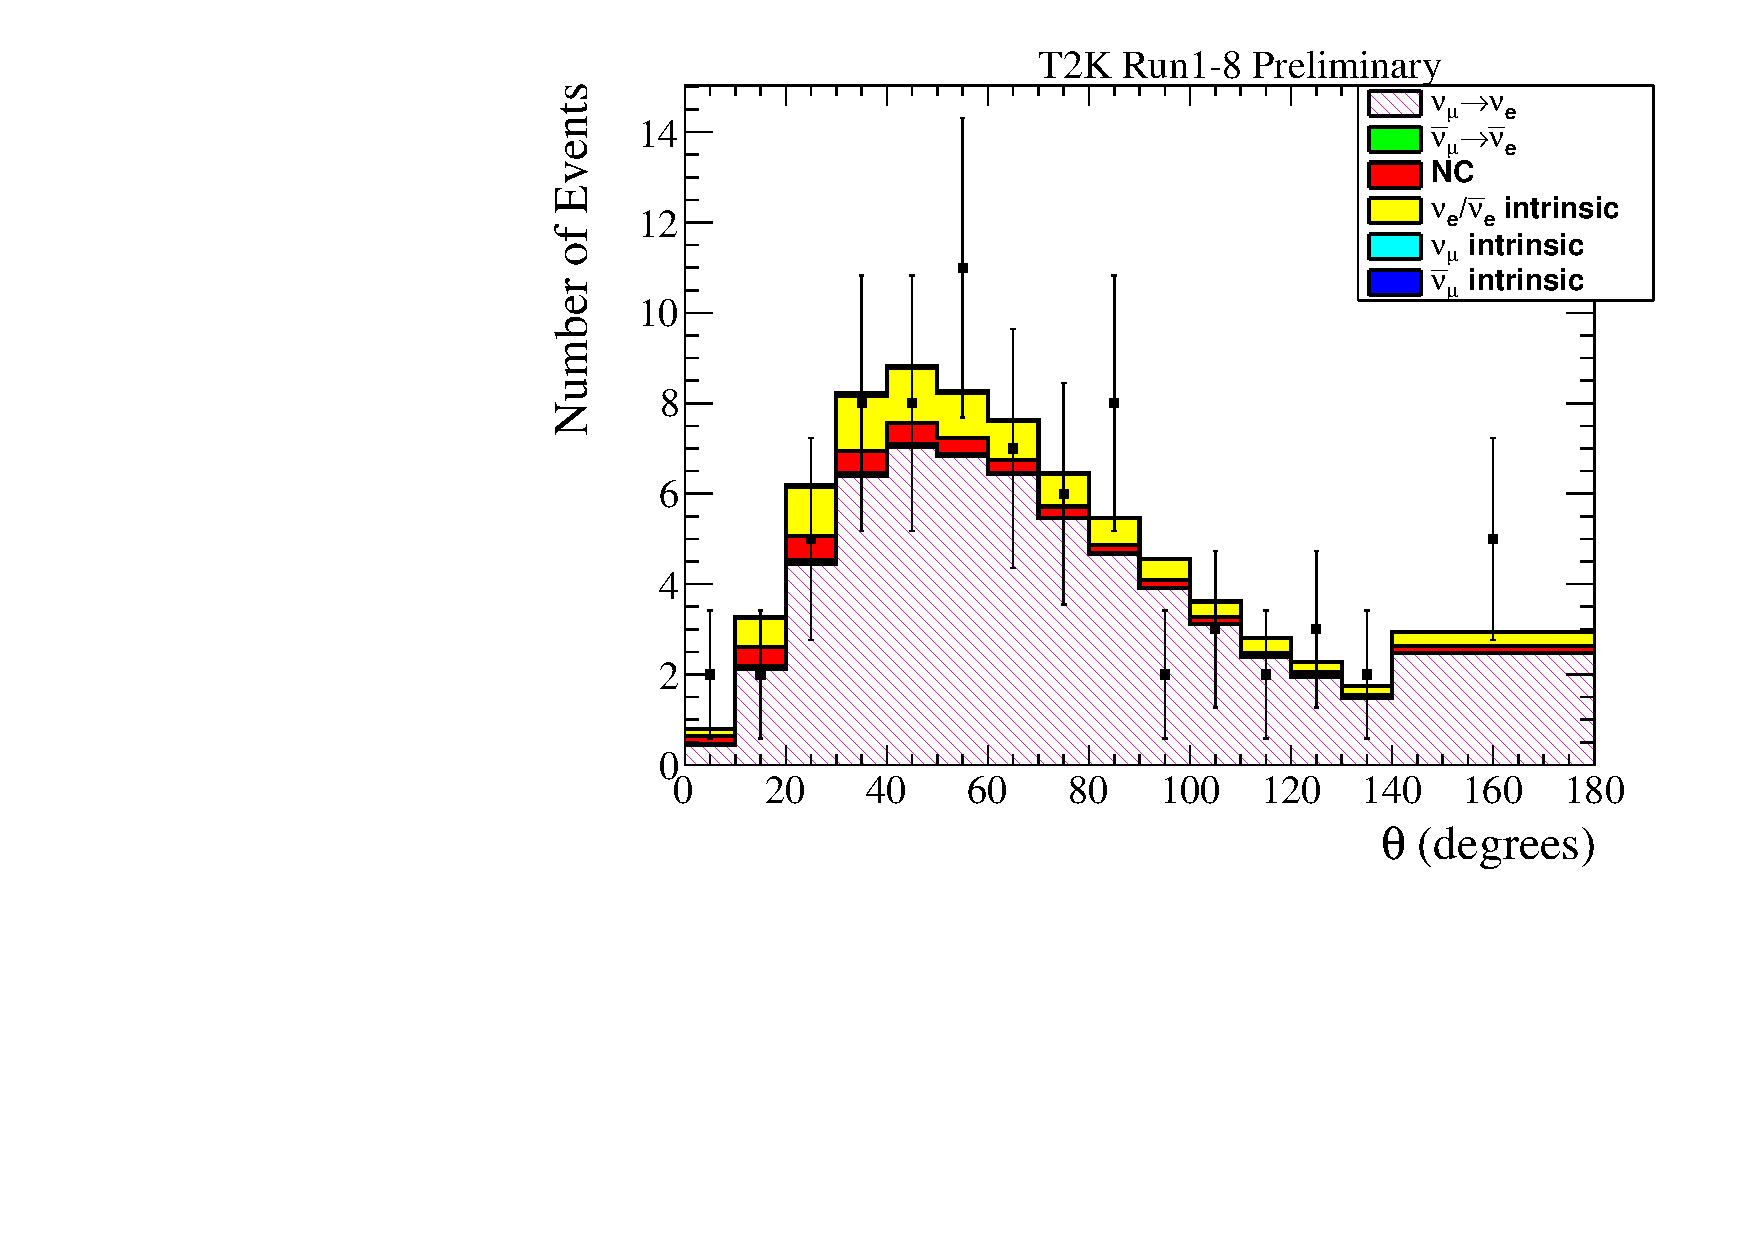
\includegraphics[width=0.9\textwidth]{spectra/2017b/theta_spectrum_osc_asimovpf_1Re_data}
		\caption{Electron-like, neutrino mode}
	\end{subfigure}

	\begin{subfigure}[b]{0.49\textwidth}
		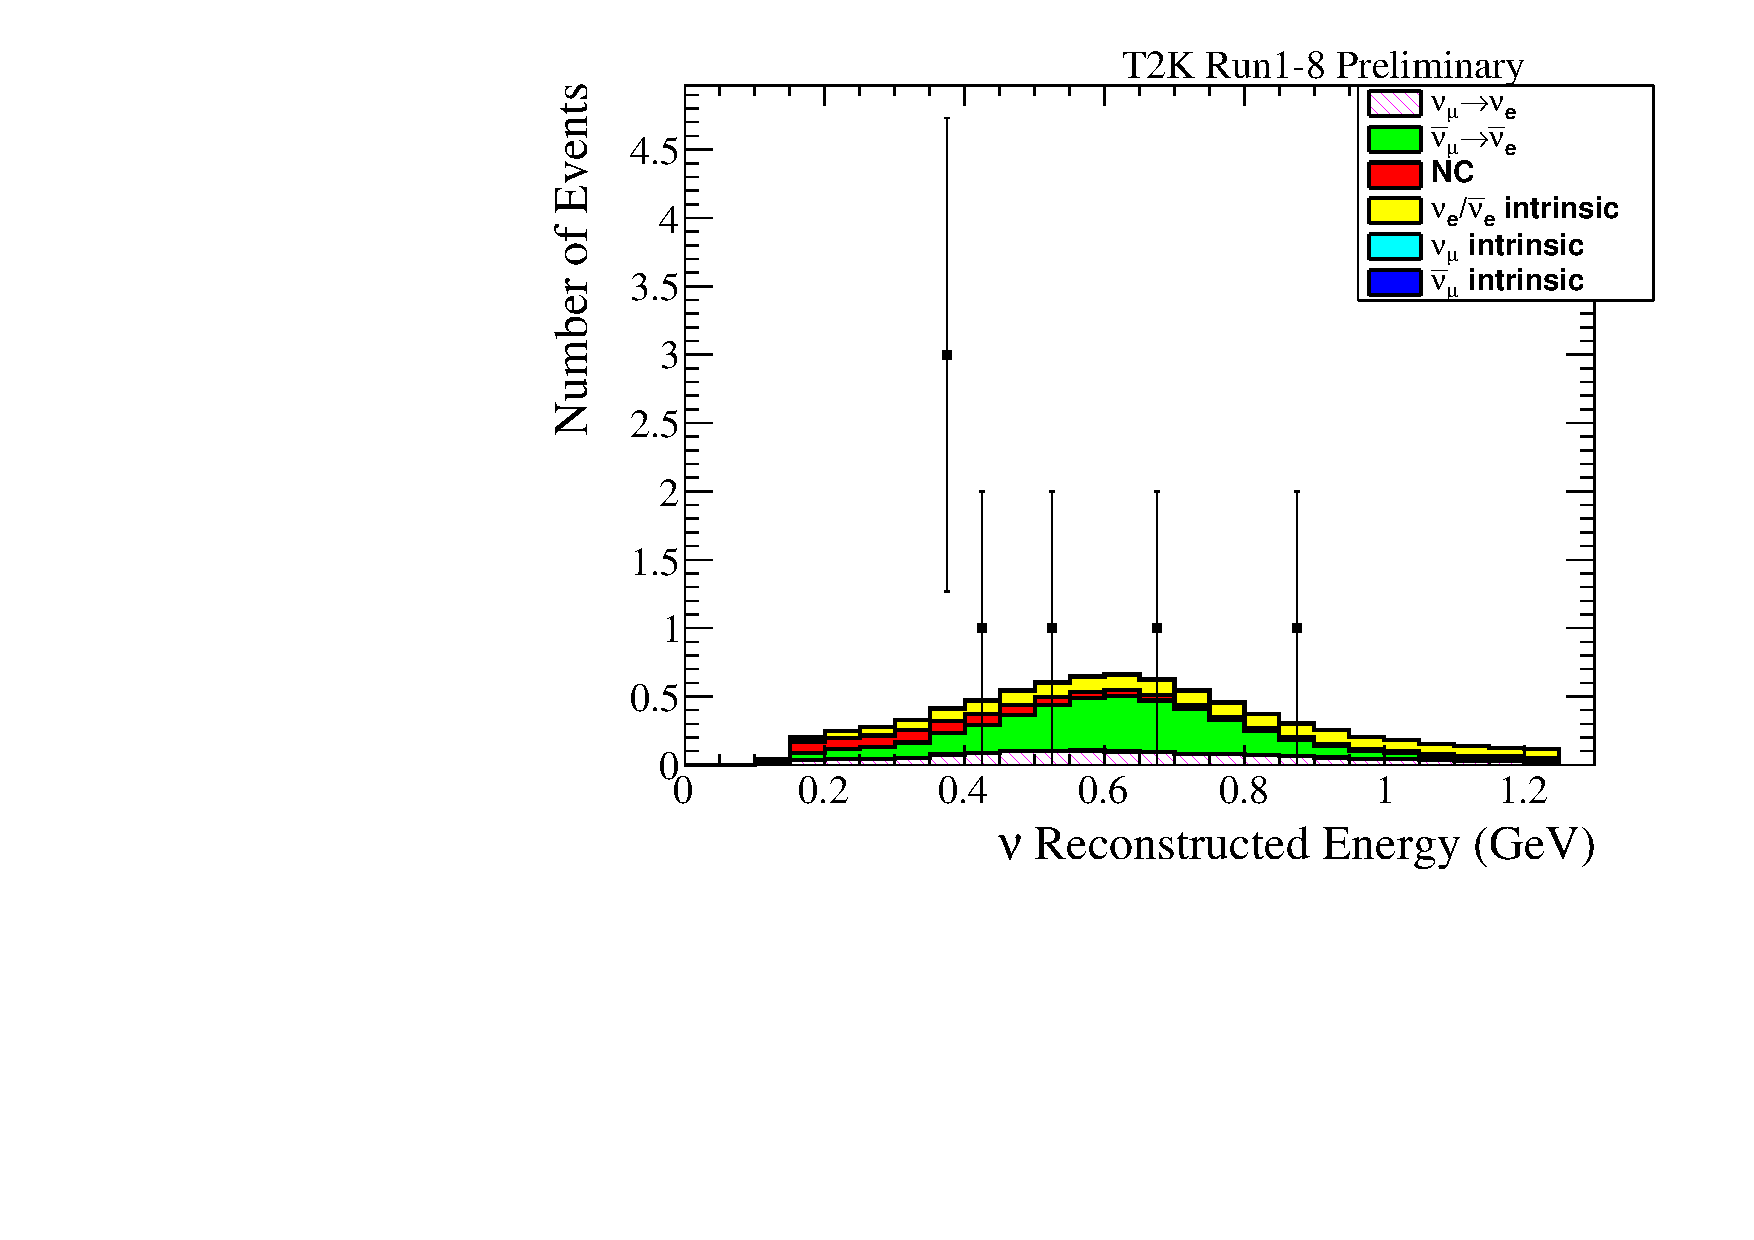
\includegraphics[width=0.9\textwidth]{spectra/2017b/erec_spectrum_osc_asimovpf_RHC1Re_data}
		\caption{Electron-like antineutrino mode}
	\end{subfigure}
	\begin{subfigure}[b]{0.49\textwidth}
		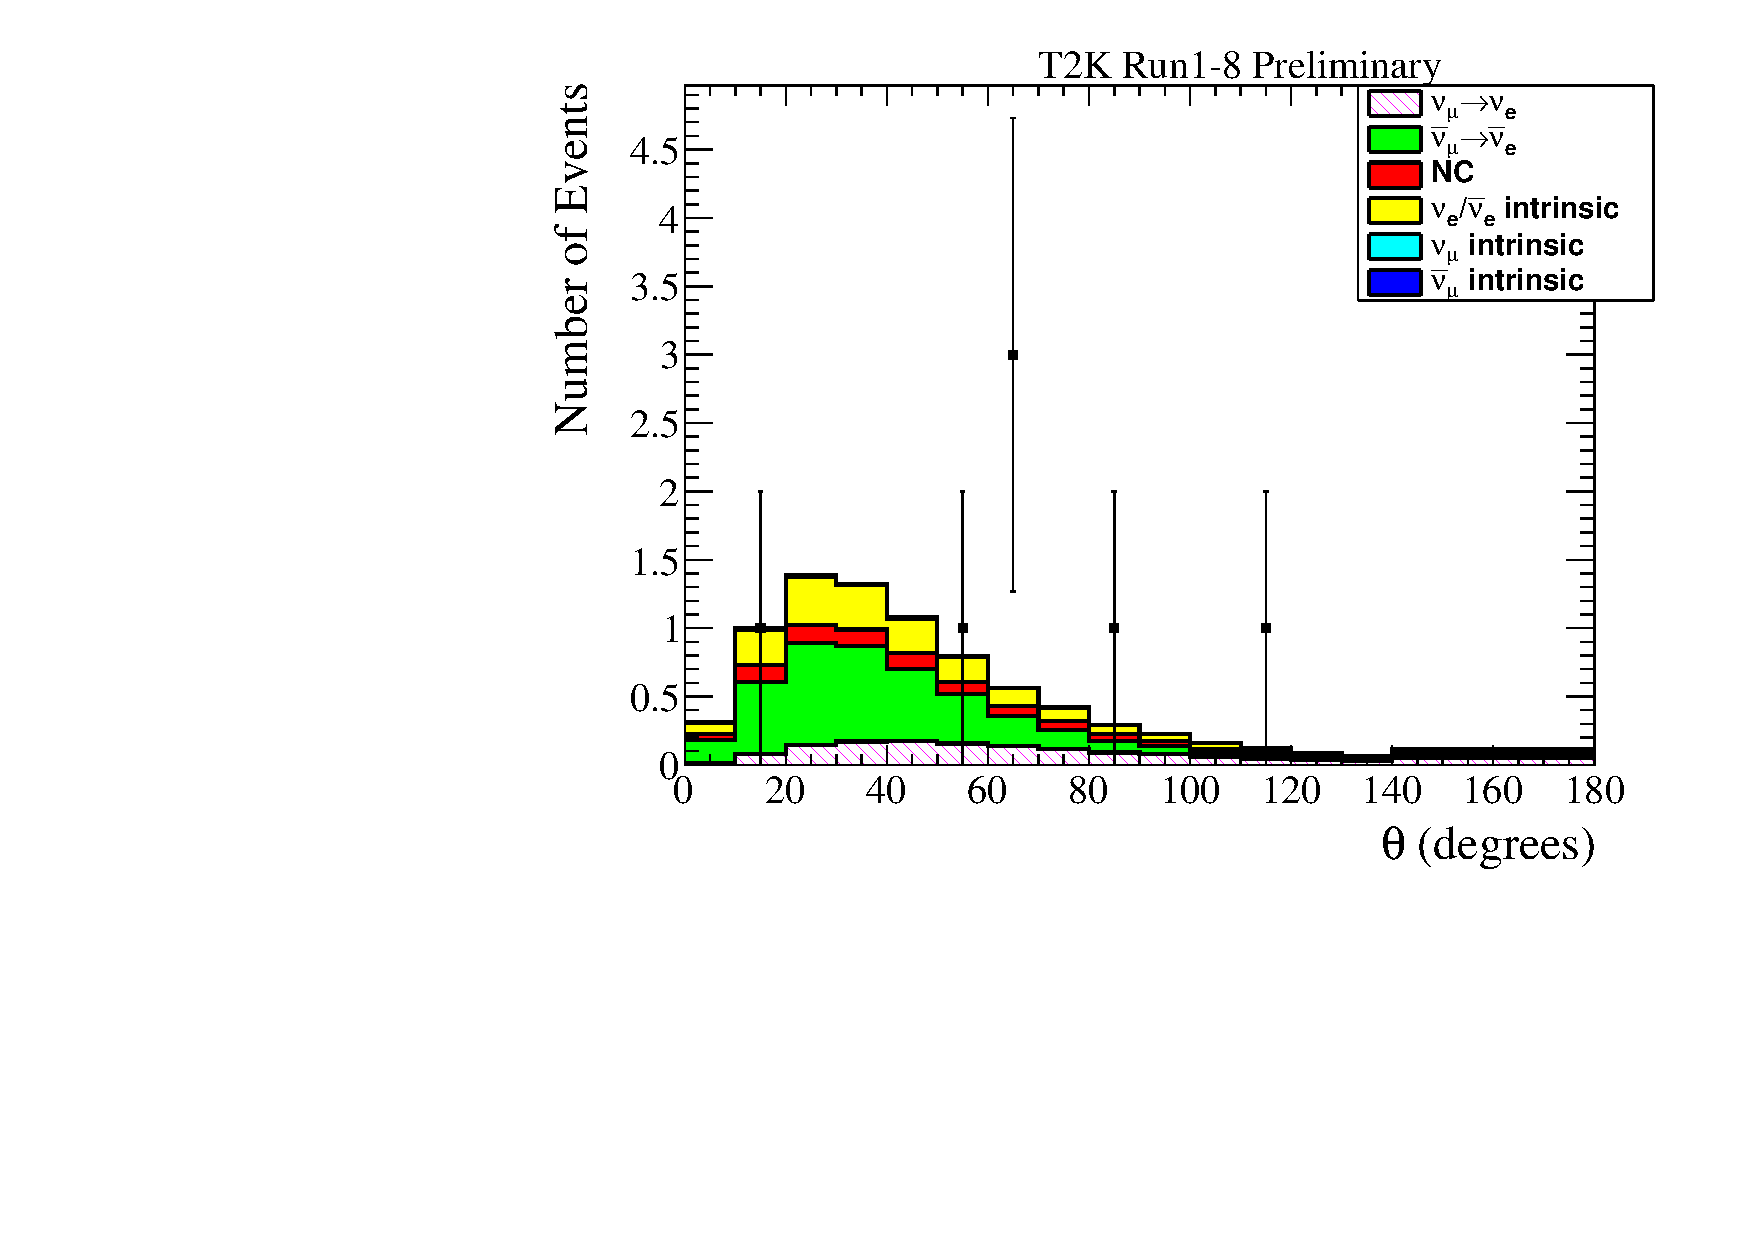
\includegraphics[width=0.9\textwidth]{spectra/2017b/theta_spectrum_osc_asimovpf_RHC1Re_data}
		\caption{Electron-like antineutrino mode}
	\end{subfigure}

	\begin{subfigure}[b]{0.49\textwidth}
		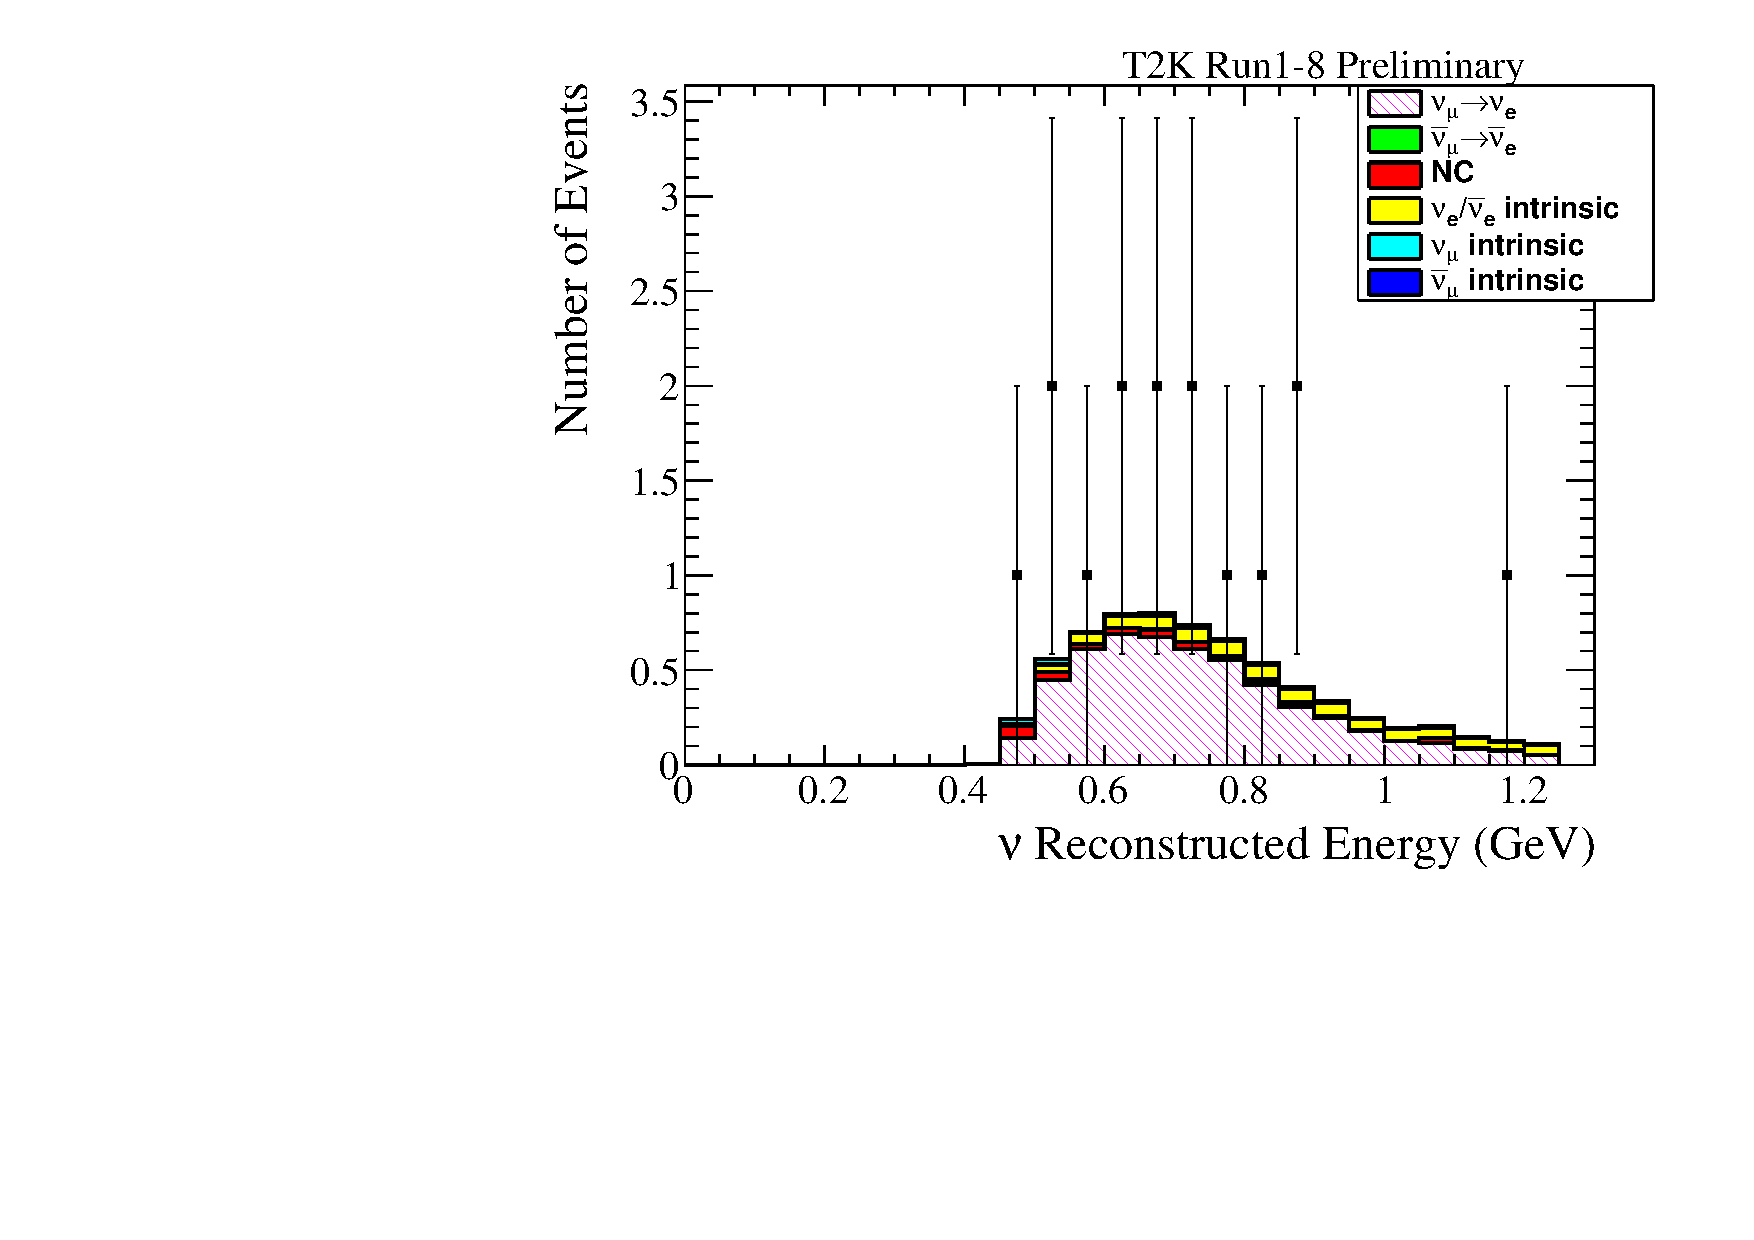
\includegraphics[width=0.9\textwidth]{spectra/2017b/erec_spectrum_osc_asimovpf_MultiRe_data}
		\caption{\nueCConepi-like, neutrino mode}
	\end{subfigure}
	\begin{subfigure}[b]{0.49\textwidth}
		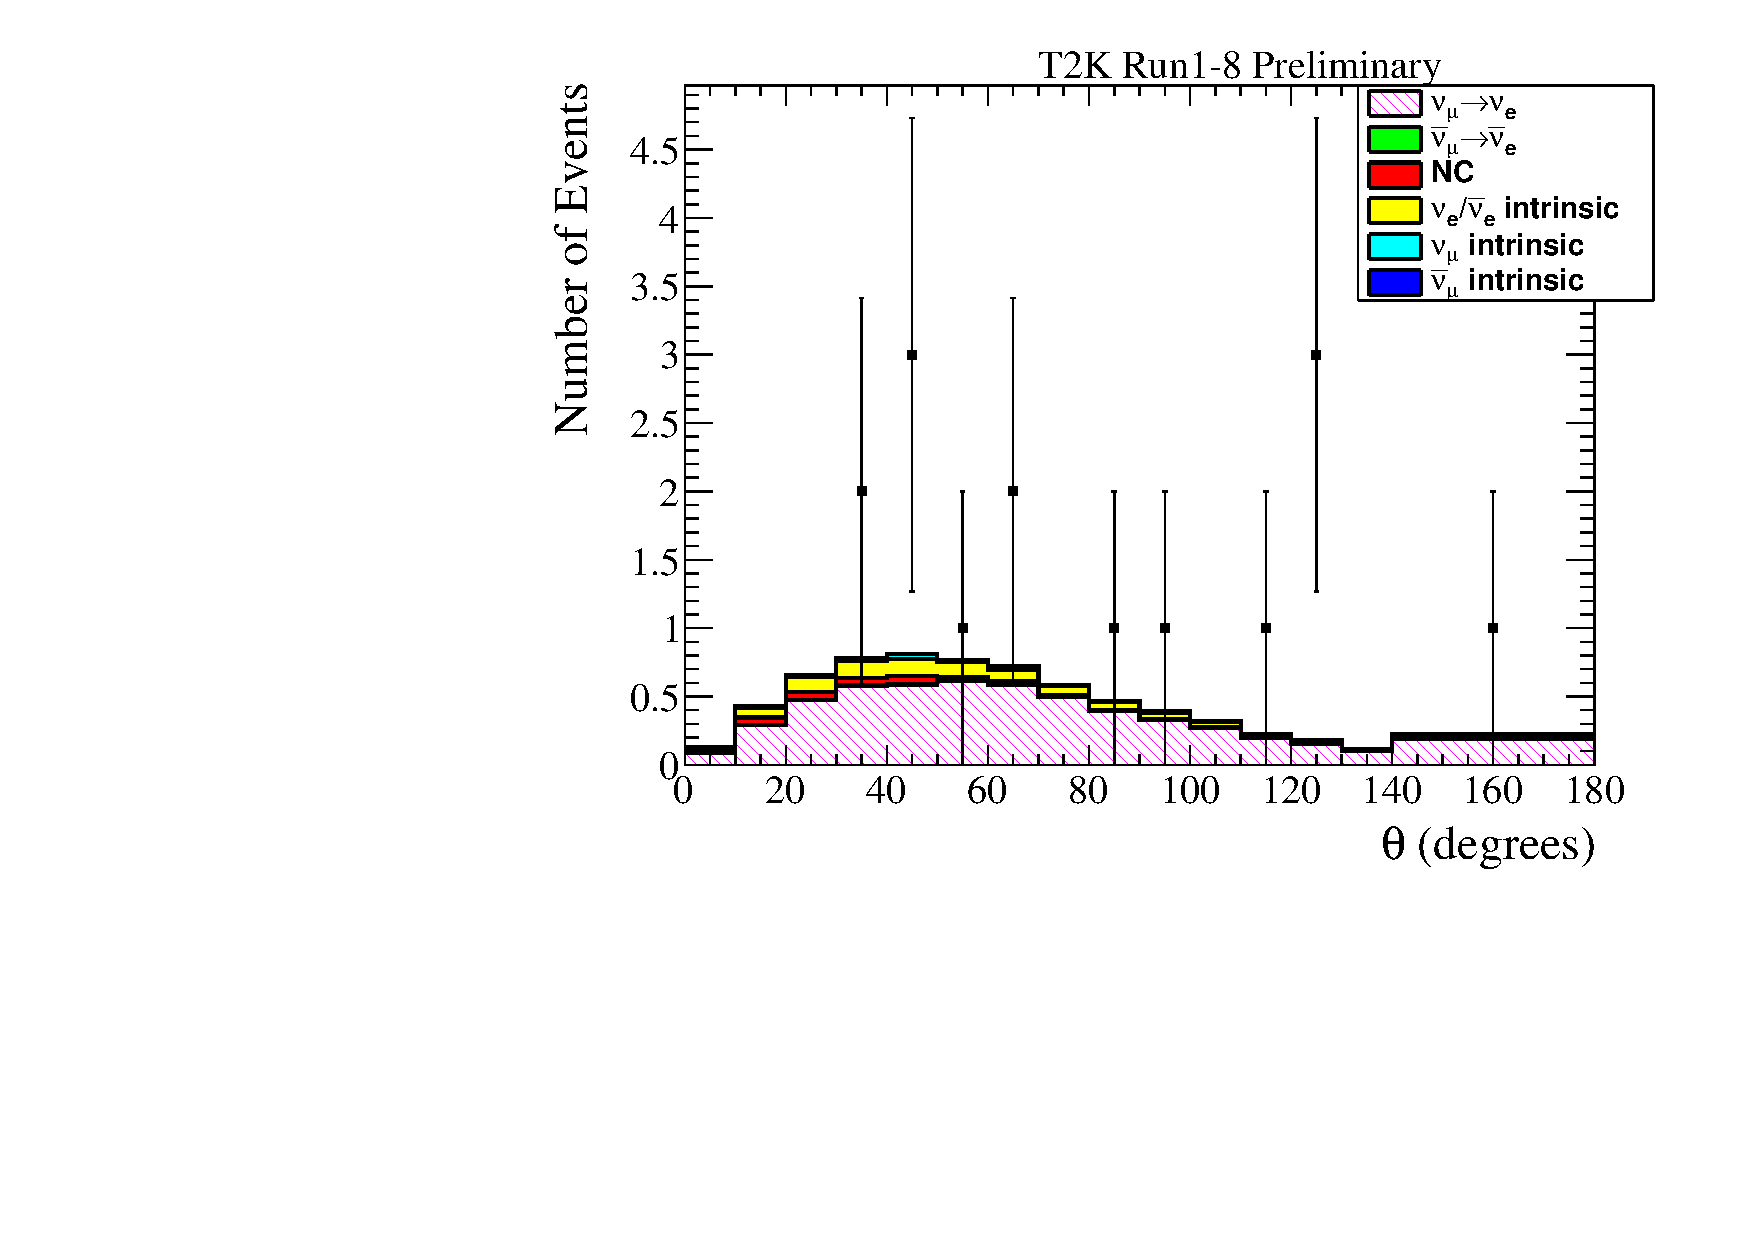
\includegraphics[width=0.9\textwidth]{spectra/2017b/theta_spectrum_osc_asimovpf_MultiRe_data}
		\caption{\nueCConepi-like, neutrino mode}
	\end{subfigure}
	\caption {
		Predicted spectra and observed events (points). The $e$-like, including \nueCConepi, distributions are functions of both the reconstructed neutrino energy and the reconstructed angle between the outgoing lepton and the neutrino direction, with the projections in each variable shown here. The distributions correspond to the statistics collected in the full \RunPeriod data set. The spectra are generated with the systematic parameters described in \cref{sec:systematics} and the oscillation parameters corresponding to the best-fit values from the data fit (solar parameters at PDG 2016).
	}
	\label{fig:asimovpf_spectra_mc_data_elike_1D_2017b}
\end{figure*}
\clearpage

The best-fit values and $1\sigma$ ranges for each oscillation parameter are shown in \cref{tab:data_bestfit_2017b} for normal hierarchy (which is preferred in all data fits). The $1\sigma$ ranges are extracted for each oscillation parameter from the 1-dimensional $\Delta \chi^2$ distributions shown in \crefrange{fig:dcp_data_2017b}{fig:dmsq23_data_2017b}.

The 1-dimensional contours are plotted with respect to the global minimum from normal and inverted hierarchies, while the 2-dimensional confidence intervals are shown drawing the normal and inverted hierarchy contours independently, i.e. each contour is produced with respect to the global minimum under that hierarchy hypothesis.

\begin{table}
\centering
\begin{tabular}{| c | c | c | c | c | c |}
\hline
Parameter & Reactor & Best-fit (NH) & $\pm1\sigma$ (NH) & Best-fit (IH) & $\pm1\sigma$ (IH) \\
\hline
\deltacp & Yes & \BestFitDeltacpwRCb & [\MOneSigmaDeltacpwRCb,\POneSigmaDeltacpwRCb] & \BestFitDeltacpwRCIHb & [\MOneSigmaDeltacpwRCIHb,\POneSigmaDeltacpwRCIHb] \\
\deltacp & No & \BestFitDeltacpwoRCb & [\MOneSigmaDeltacpwoRCb,\POneSigmaDeltacpwoRCb] & \BestFitDeltacpwoRCIHb & [\MOneSigmaDeltacpwoRCIHb,\POneSigmaDeltacpwoRCIHb] \\
\ssqthonethree & No & \BestFitMixingOneThreewoRCb & [\MOneMixingOneThreewoRCb,\POneMixingOneThreewoRCb] & \BestFitMixingOneThreewoRCIHb & [\MOneMixingOneThreewoRCIHb,\POneMixingOneThreewoRCIHb] \\
\ssqthtwothree & Yes & \BestFitMixingTwoThreewRCb & [\MOneMixingTwoThreewRCb,\POneMixingTwoThreewRCb] & \BestFitMixingTwoThreewRCIHb & [\MOneMixingTwoThreewRCIHb,\POneMixingTwoThreewRCIHb] \\
\dmsqtwothree or \dmsqonethree & Yes & \BestFitDmTwoThreewRCb & [\MOneDmTwoThreewRCb,\POneDmTwoThreewRCb] & \BestFitDmTwoThreewRCIHb & [\MOneDmTwoThreewRCIHb,\POneDmTwoThreewRCIHb] \\
 ($10^{-3}\text{ eV}^2\text{/c}^4$) & & & & & \\
\hline
\end{tabular}

\caption{
The \RunPeriod measured oscillation parameter best-fit and the $\pm 1\sigma$ intervals are shown for normal and inverted hierarchies with respect to the hierarchy best-fit. The $\pm 1\sigma$ interval is obtained by using the constant $\Delta \chi^2$ method. For each parameter normal hierarchy is the global best-fit.
}
\label{tab:data_bestfit_2017b}
\end{table}

\clearpage

\subsubsection{Results for \appearance}
In \cref{fig:ssqth13_vs_dcp_data_2017b} the result for \appearance with reactor constraint and T2K only is shown.

\begin{figure*}[htb]
	\center
	\begin{subfigure}[b]{0.49\textwidth}
		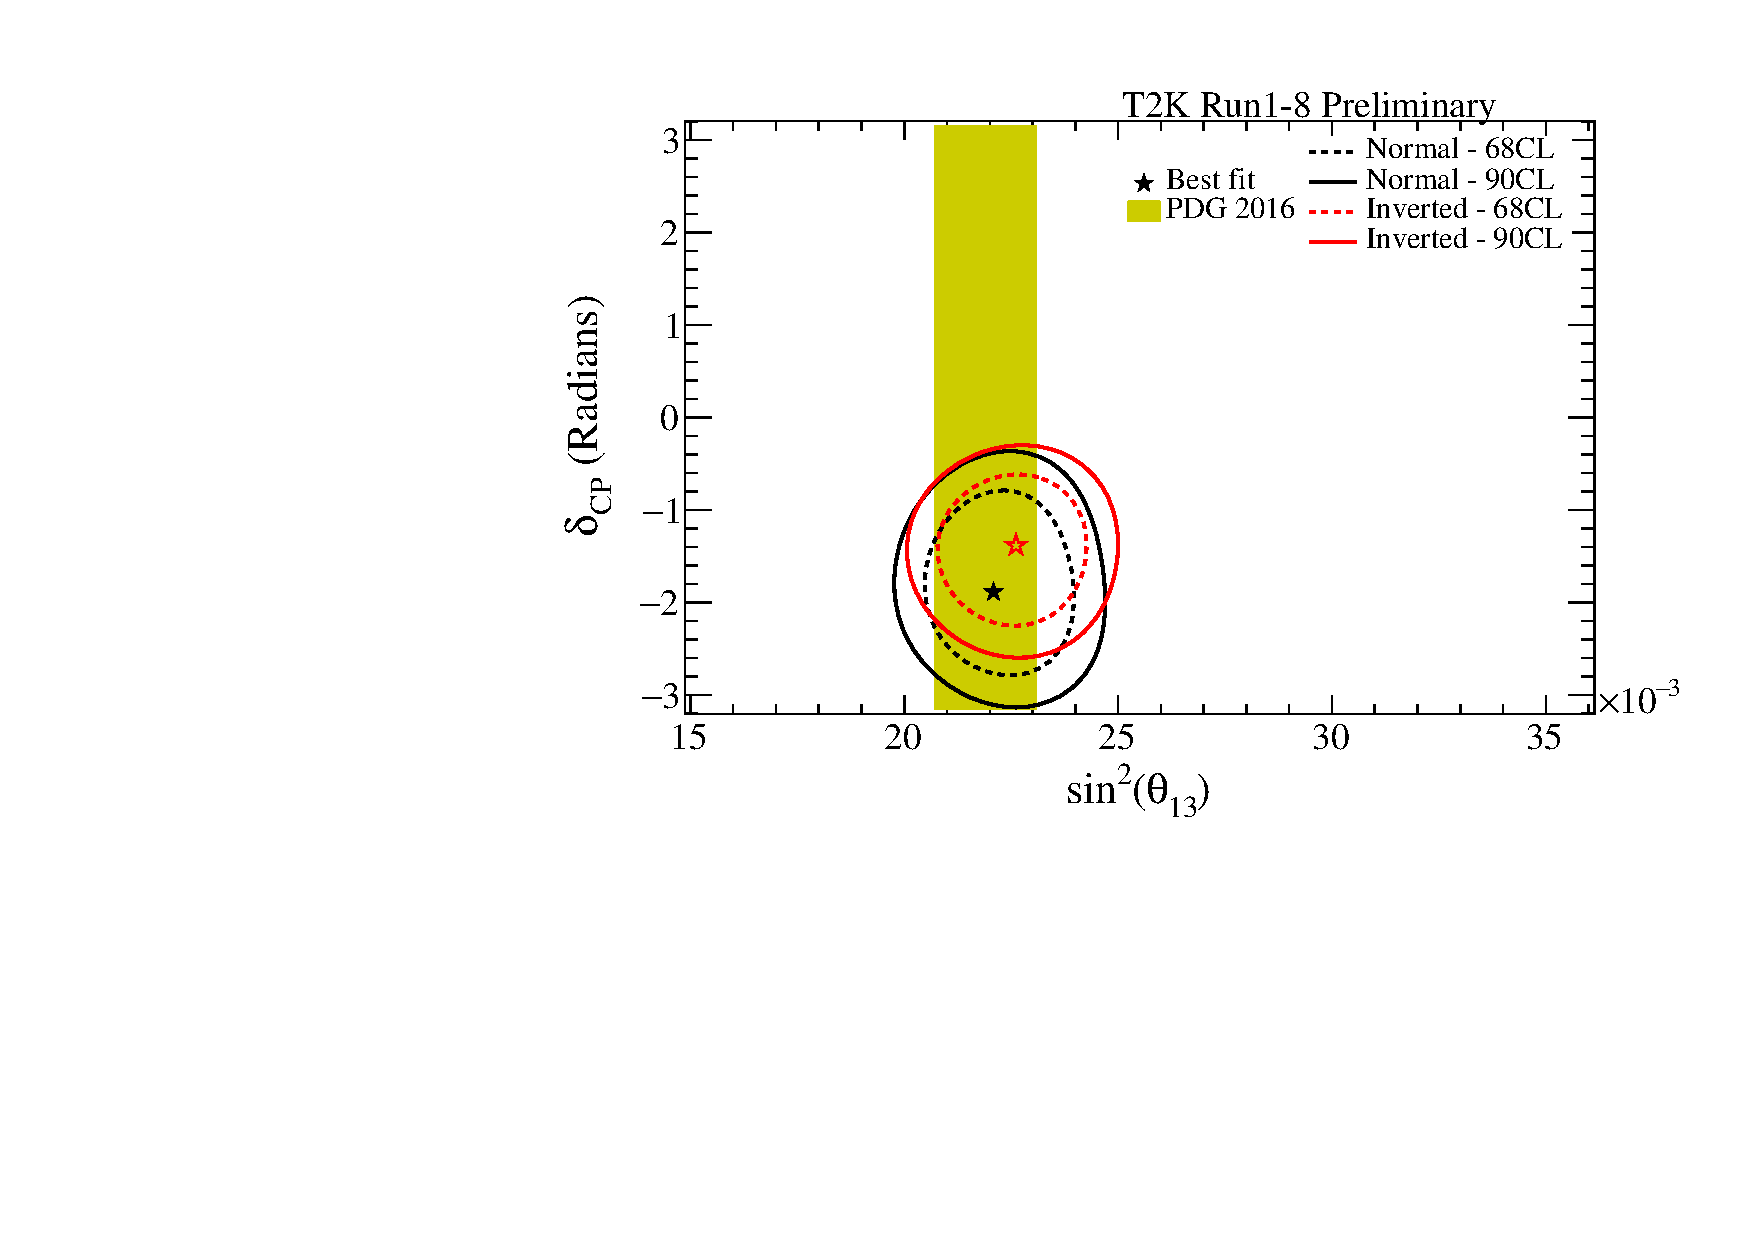
\includegraphics[width=0.9\textwidth]{data/reactor/2017b/mixing13_deltacp_data_reactor_global}
		\caption{\appearance with reactor constraint}
	\end{subfigure}
	\begin{subfigure}[b]{0.49\textwidth}
		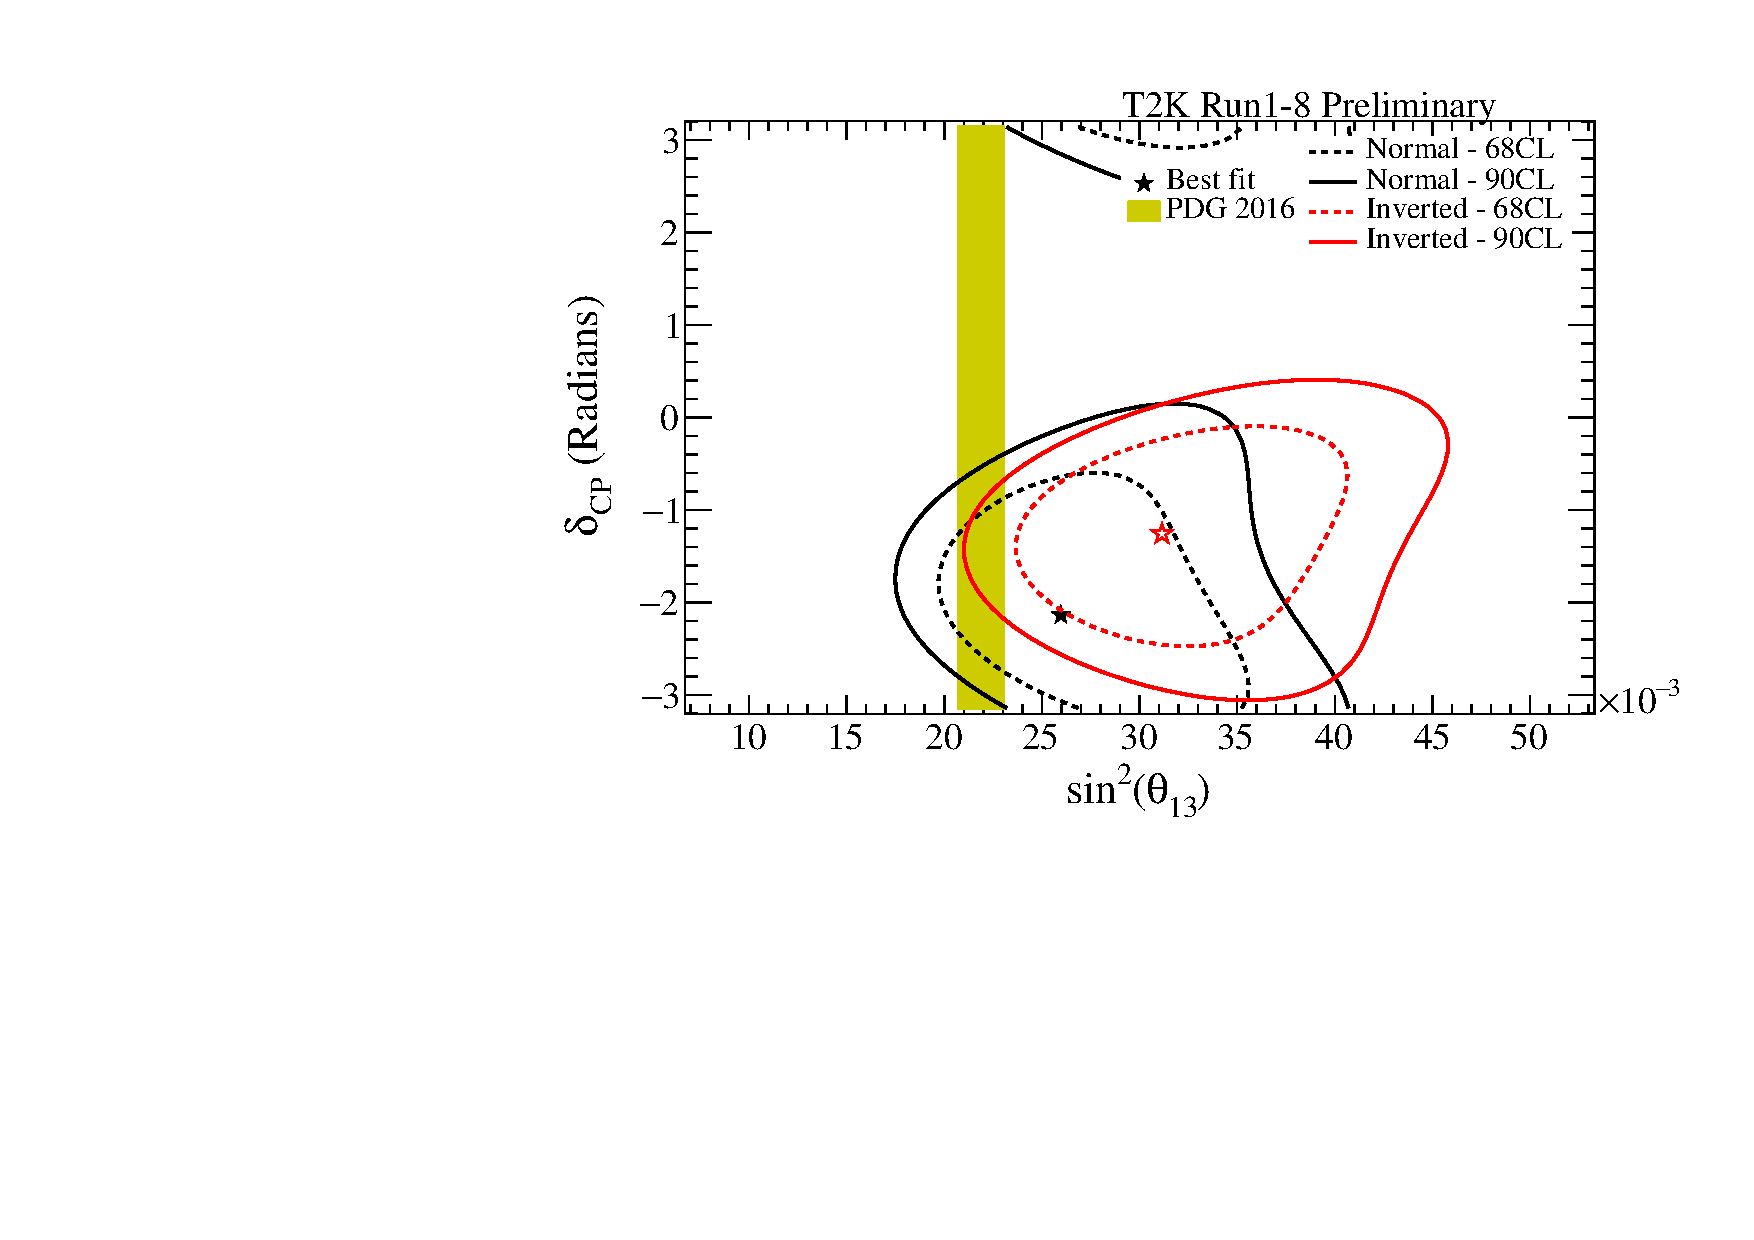
\includegraphics[width=0.9\textwidth]{data/t2k/2017b/mixing13_deltacp_data_t2k_global}
		\caption{\appearance T2K only}
	\end{subfigure}
	\caption {
		Contours at 68\% and 90\% CL for \appearance with and without reactor constraint. Normal and inverted hierarchy contours are independent. All 5 samples were used to produce these fits.
	}
	\label{fig:ssqth13_vs_dcp_data_2017b}
\end{figure*}

\subsubsection{Results for \disappearance}

The result for \disappearance with reactor constraint and T2K only is shown in fig.~\ref{fig:ssqth23_vs_dmsq23_data_2017b}.

\begin{figure*}[htb]
	\center
	\begin{subfigure}[b]{0.49\textwidth}
		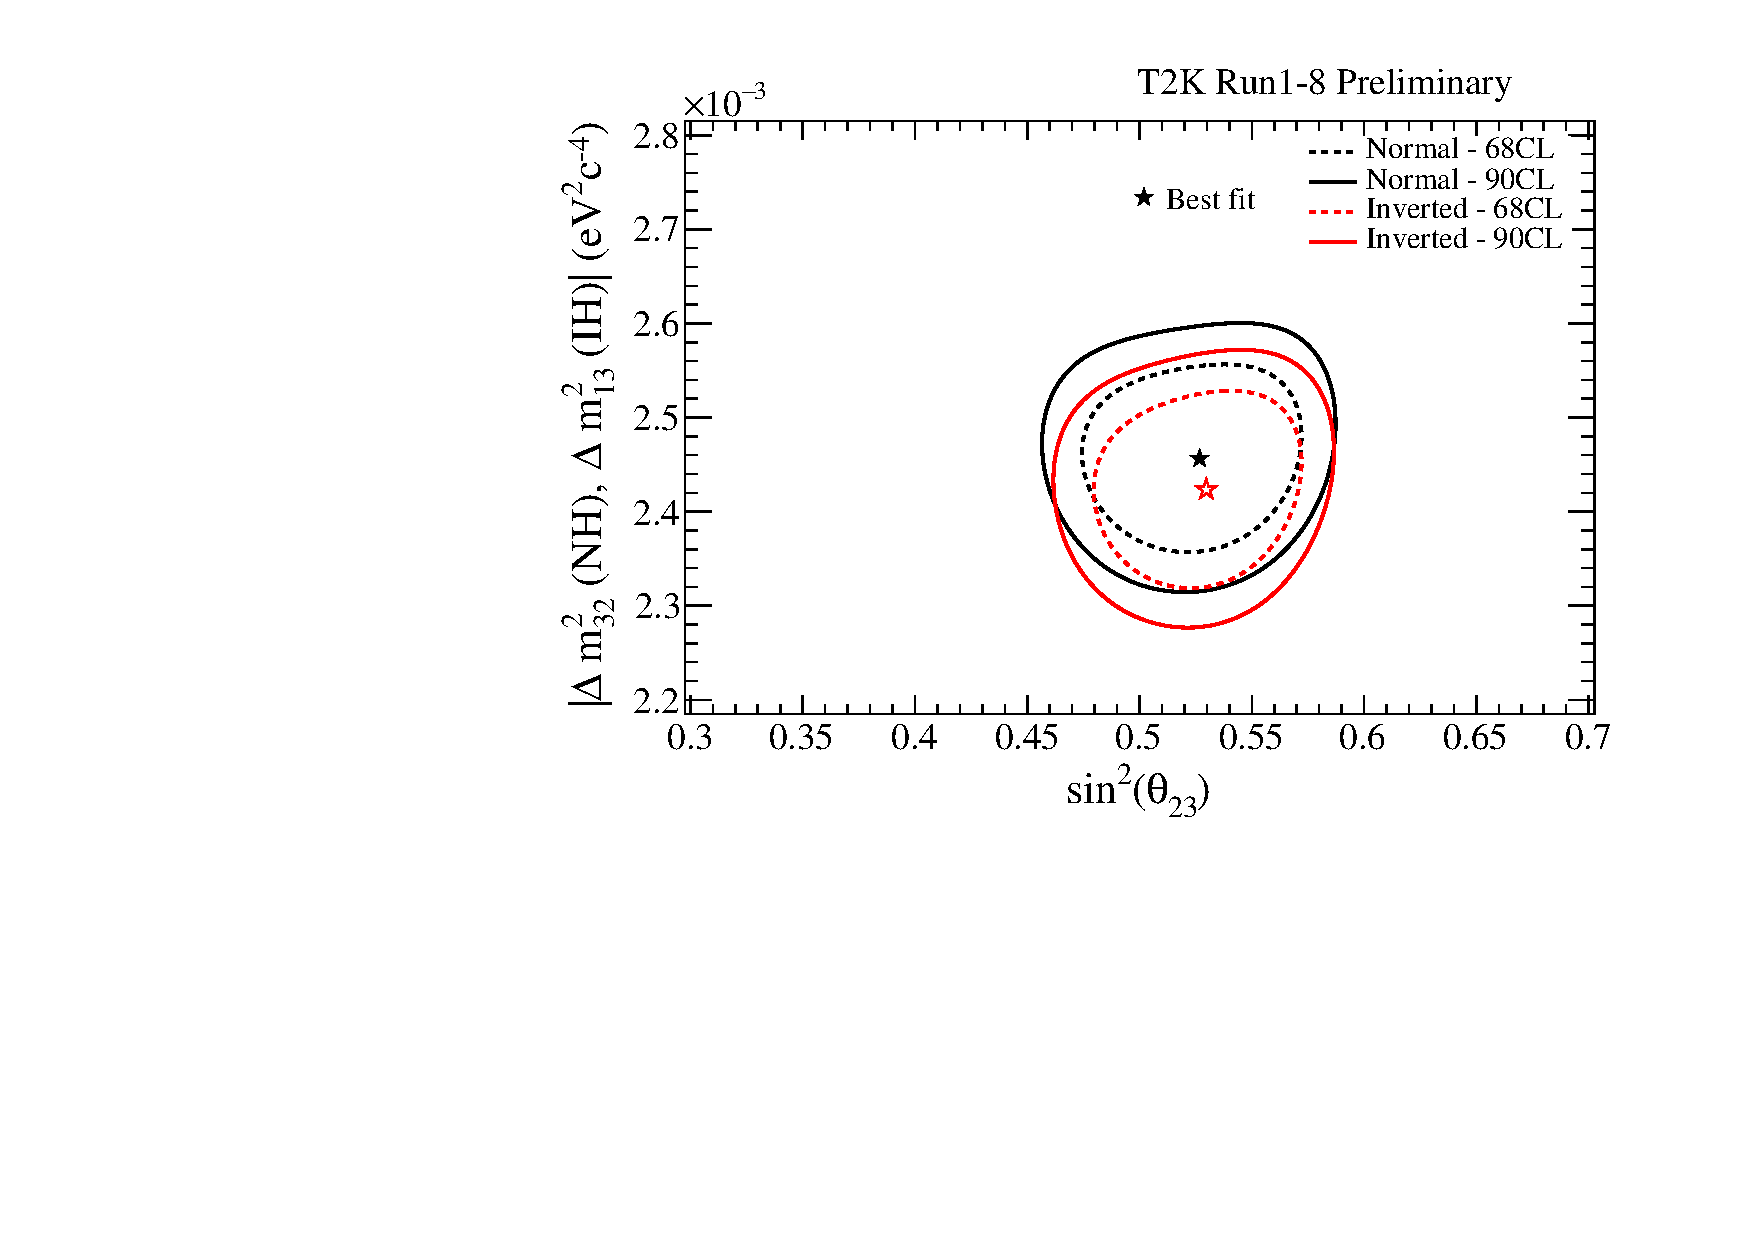
\includegraphics[width=0.9\textwidth]{data/reactor/2017b/mixing23_dmsq23_data_reactor_global}
		\caption{\disappearance with reactor constraint}
	\end{subfigure}
	\begin{subfigure}[b]{0.49\textwidth}
		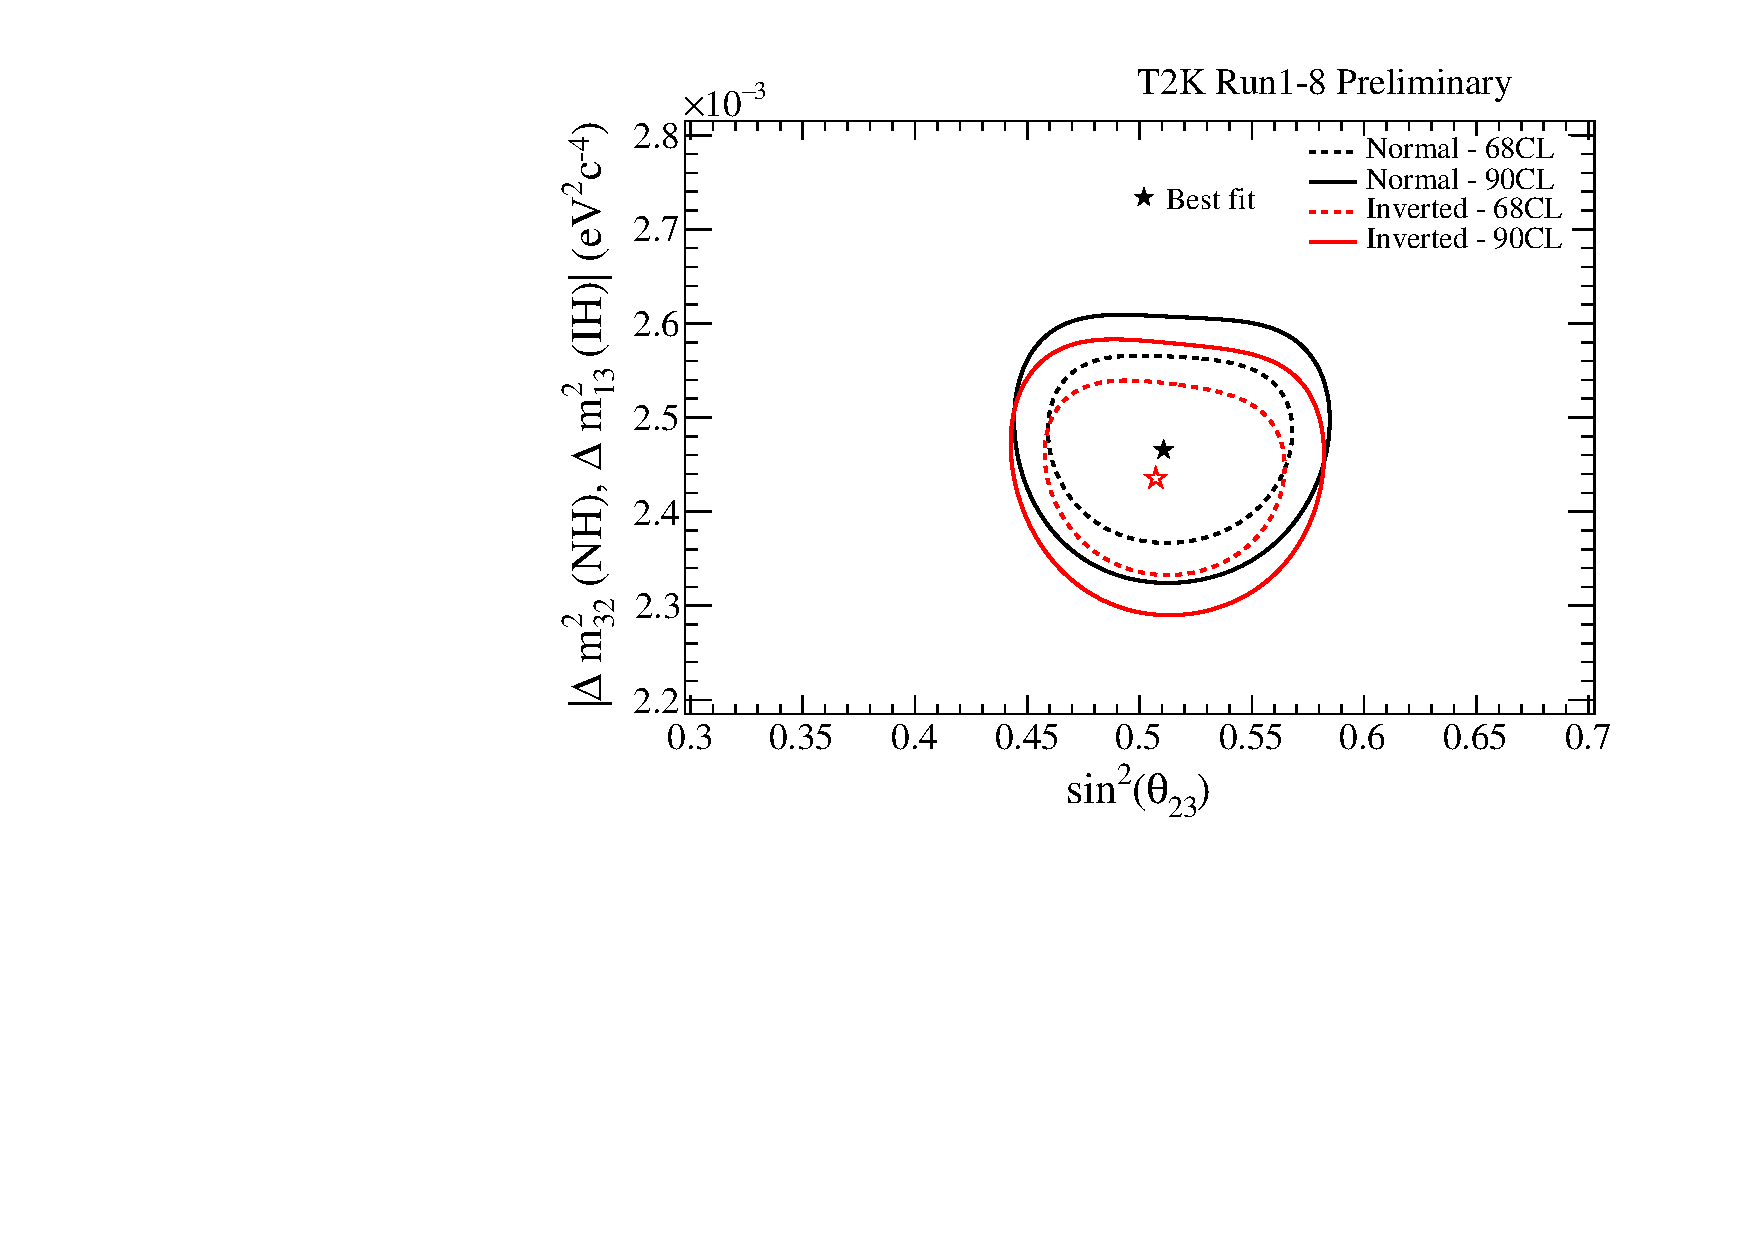
\includegraphics[width=0.9\textwidth]{data/t2k/2017b/mixing23_dmsq23_data_t2k_global}
		\caption{\disappearance T2K only}
	\end{subfigure}
	\caption {
		Contours at 68\% and 90\% CL for \disappearance with and without reactor constraint. Normal and inverted hierarchy contours are independent. All 5 samples were used to produce these fits.
	}
	\label{fig:ssqth23_vs_dmsq23_data_2017b}
\end{figure*}

\clearpage

\subsubsection{Results for \deltacp}

The result for \deltacp with reactor constraint and T2K only is shown in fig.~\ref{fig:dcp_data_2017b}.

\begin{figure*}[htb]
	\center
	\begin{subfigure}[b]{0.49\textwidth}
		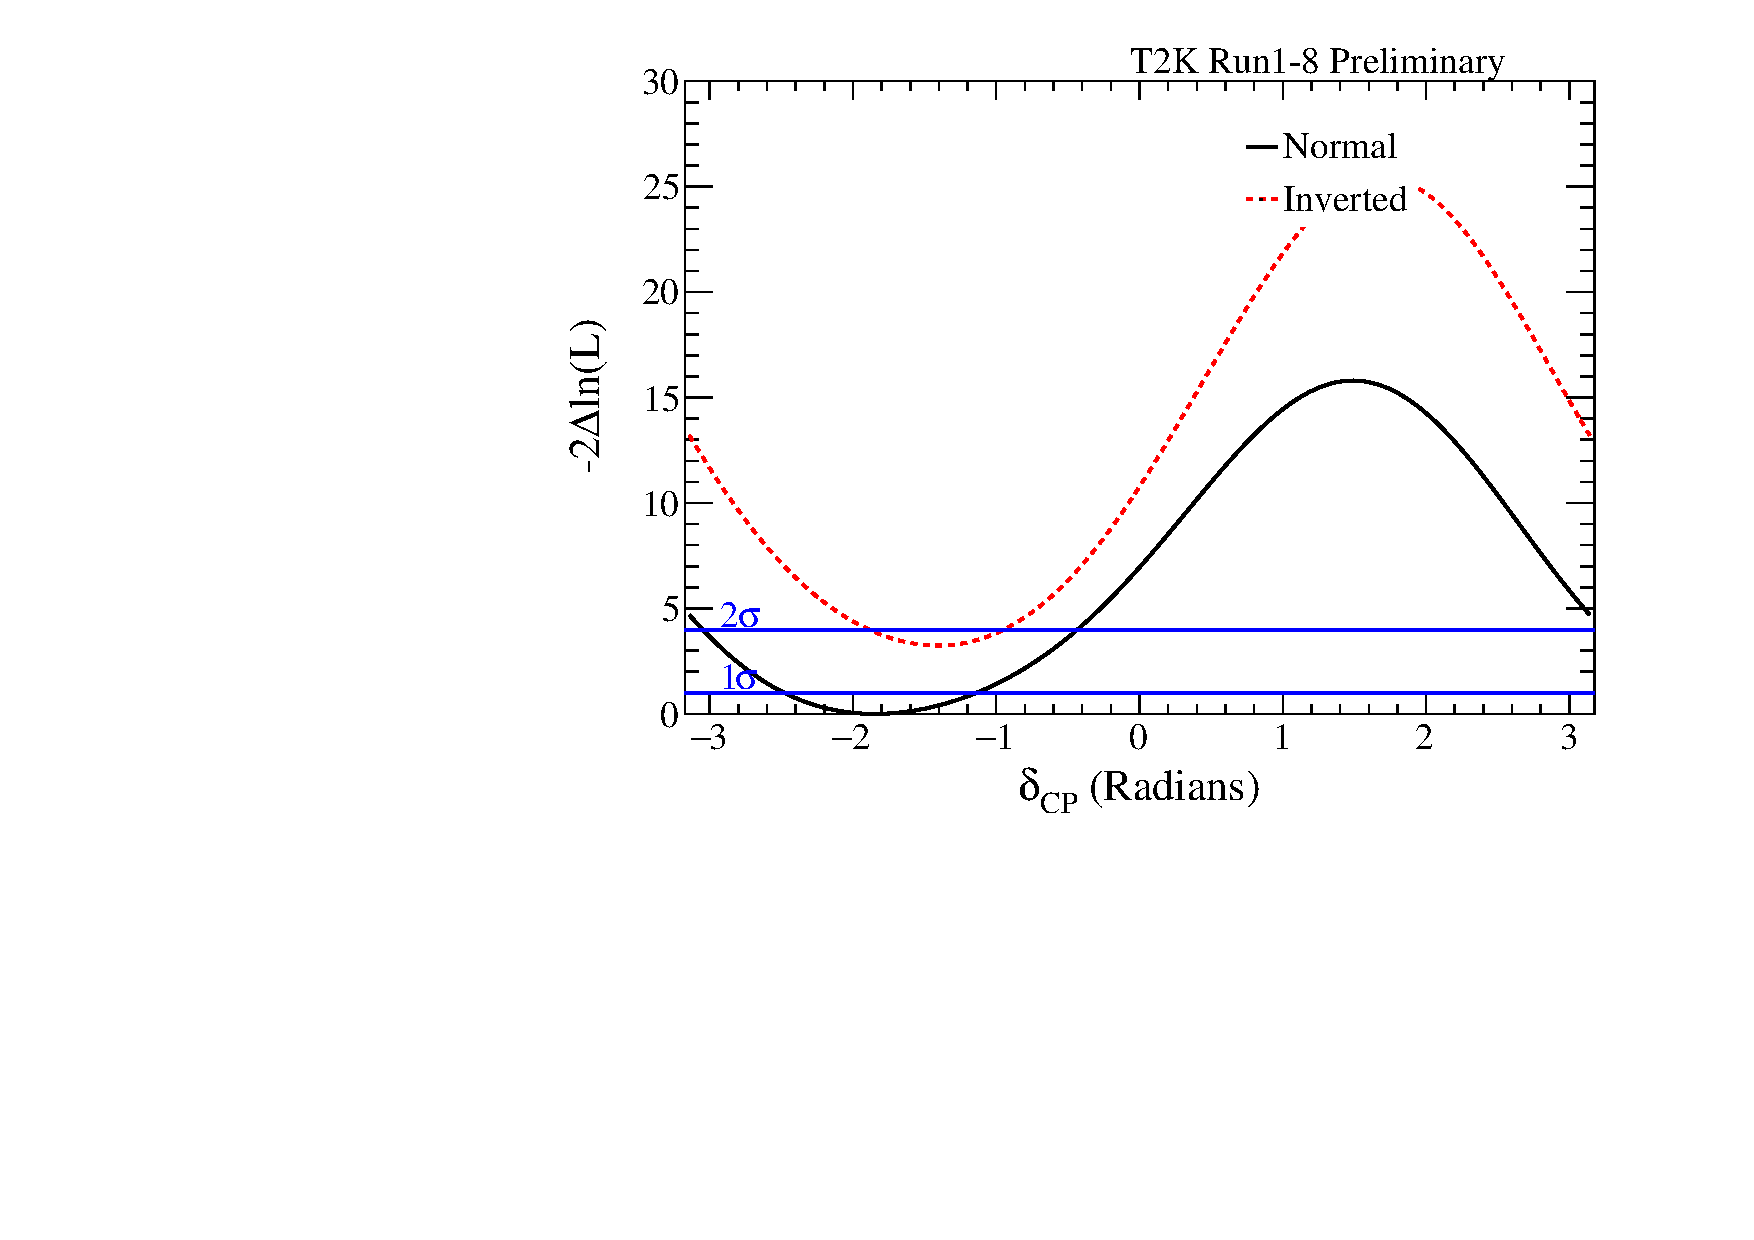
\includegraphics[width=0.9\textwidth]{data/reactor/2017b/deltacp_data_reactor_global}
		\caption{\deltacp with reactor constraint}
	\end{subfigure}
	\begin{subfigure}[b]{0.49\textwidth}
		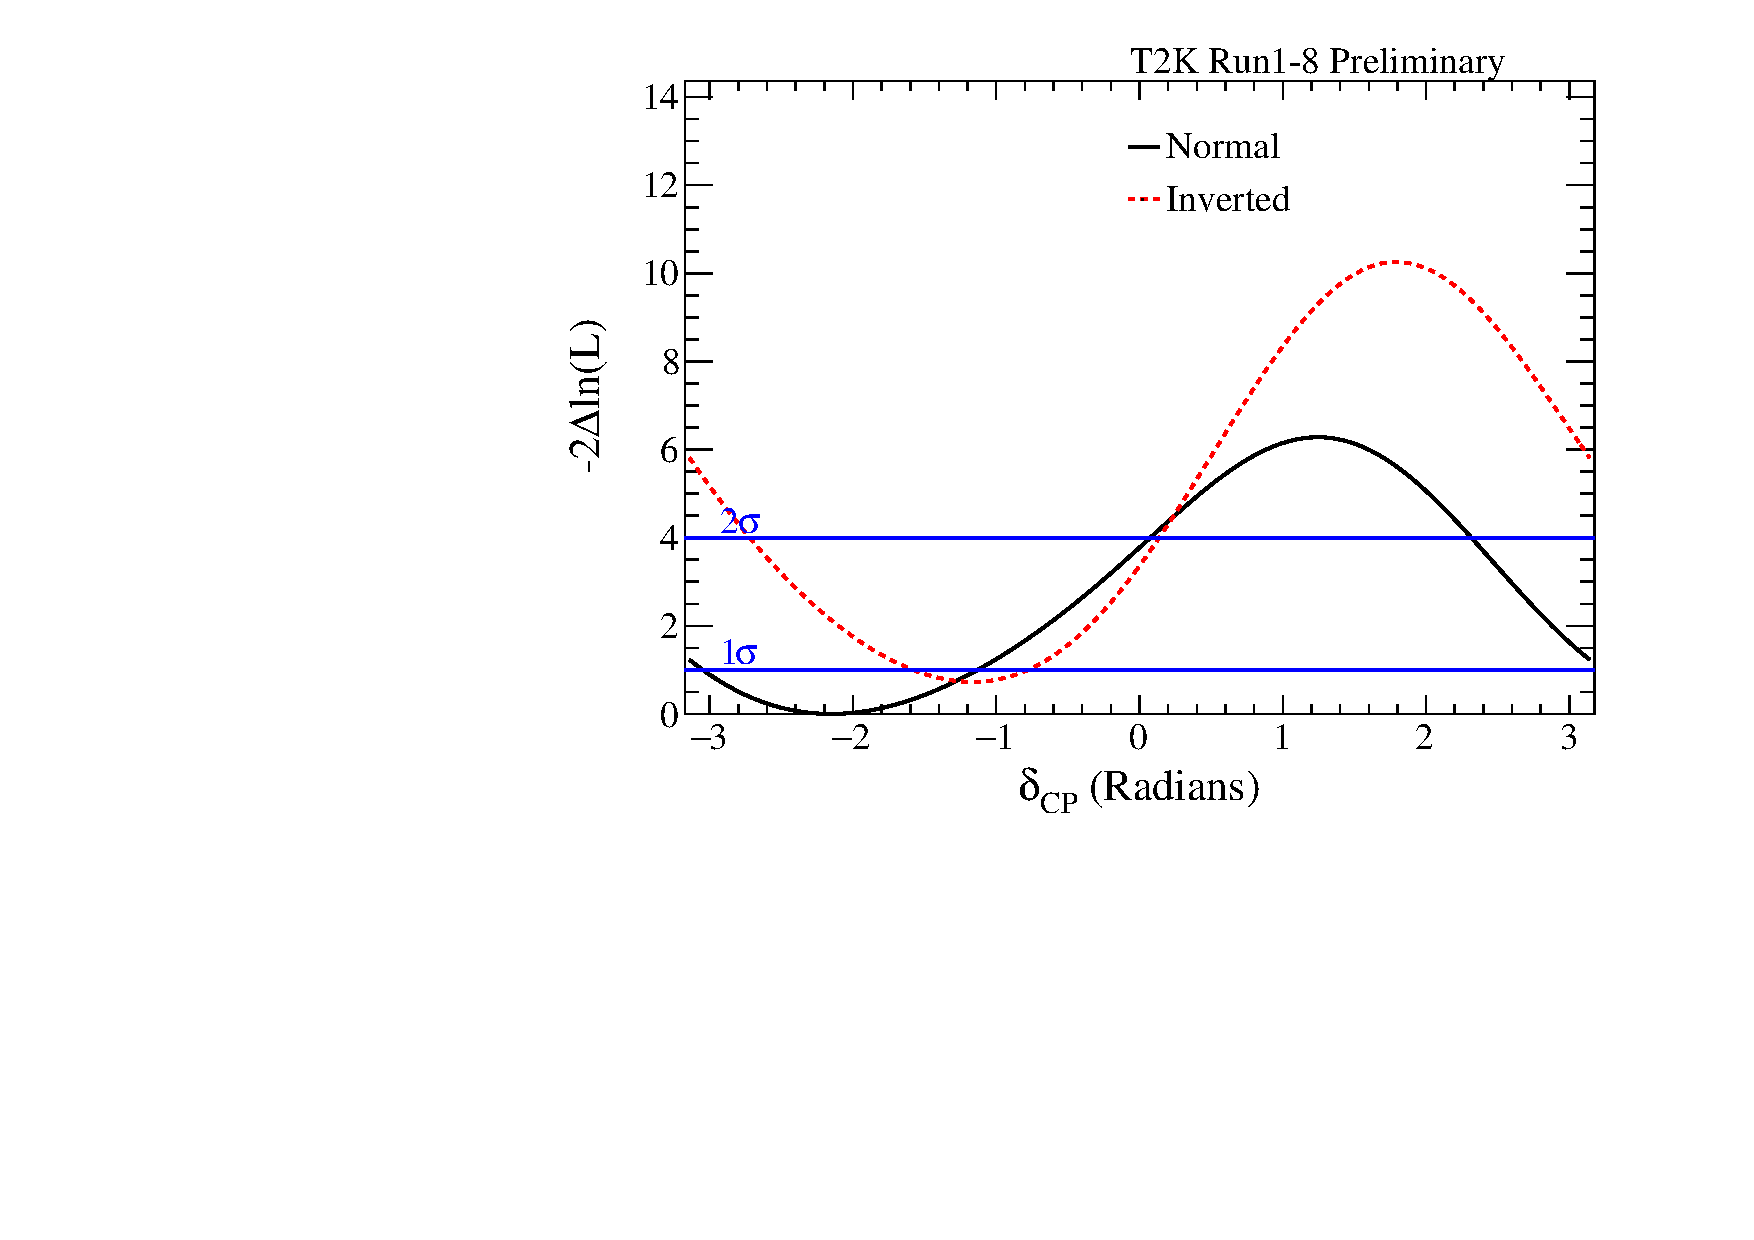
\includegraphics[width=0.9\textwidth]{data/t2k/2017b/deltacp_data_t2k_global}
		\caption{\deltacp T2K only}
	\end{subfigure}
	\caption {
		The expected $\Delta\chi^2$ distribution as a function of \deltacp with and without reactor constraint. The mass hierarchy is minimized, with normal and inverted hierarchy $\Delta\chi^2$ distributions shifted to the same global best-fit $\chi^2$ value, which is taken to be the minimum between normal and inverted hierarchy. All 5 samples were used to produce these fits.
	}
	\label{fig:dcp_data_2017b}
\end{figure*}

\subsubsection{Results for \ssqthonethree}

The result for \ssqthonethree (without reactor constraint) is shown in fig.~\ref{fig:th13_data_2017b}.

\begin{figure*}[htb]
	\center
	\begin{subfigure}[b]{0.49\textwidth}
		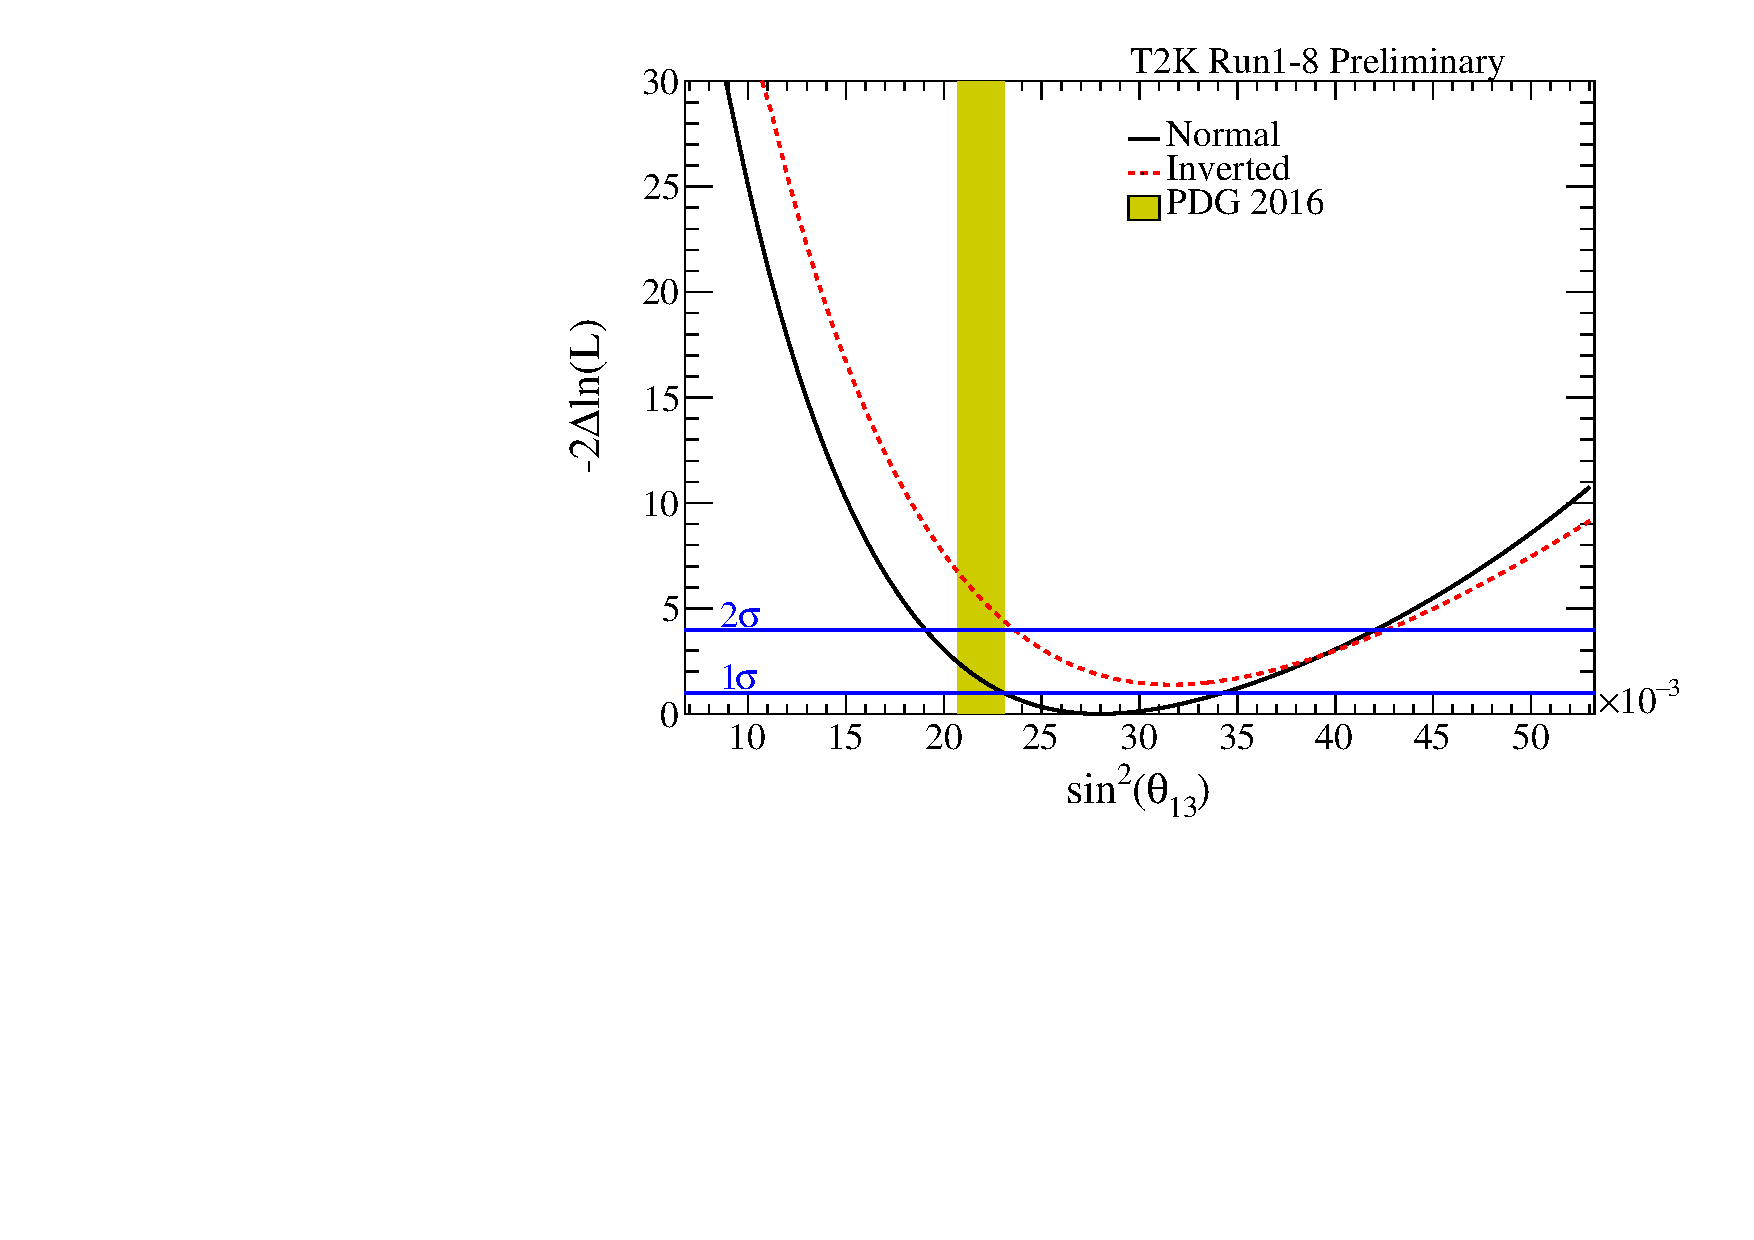
\includegraphics[width=0.9\textwidth]{data/t2k/2017b/mixing13_data_t2k_global}
		\caption{\ssqthonethree T2K only}
	\end{subfigure}
	\caption {
		The expected $\Delta\chi^2$ distribution as a function of \ssqthonethree without reactor constraint. The mass hierarchy is minimized, with normal and inverted hierarchy $\Delta\chi^2$ distributions shifted to the same global best-fit $\chi^2$ value, which is taken to be the minimum between normal and inverted hierarchy. All 5 samples were used to produce these fits.
	}
	\label{fig:th13_data_2017b}
\end{figure*}

\clearpage

\subsubsection{Results for \ssqthtwothree}

The result for \ssqthtwothree with reactor constraint and T2K only is shown in fig.~\ref{fig:th23_data_2017b}.

\begin{figure*}[htb]
	\center
	\begin{subfigure}[b]{0.49\textwidth}
		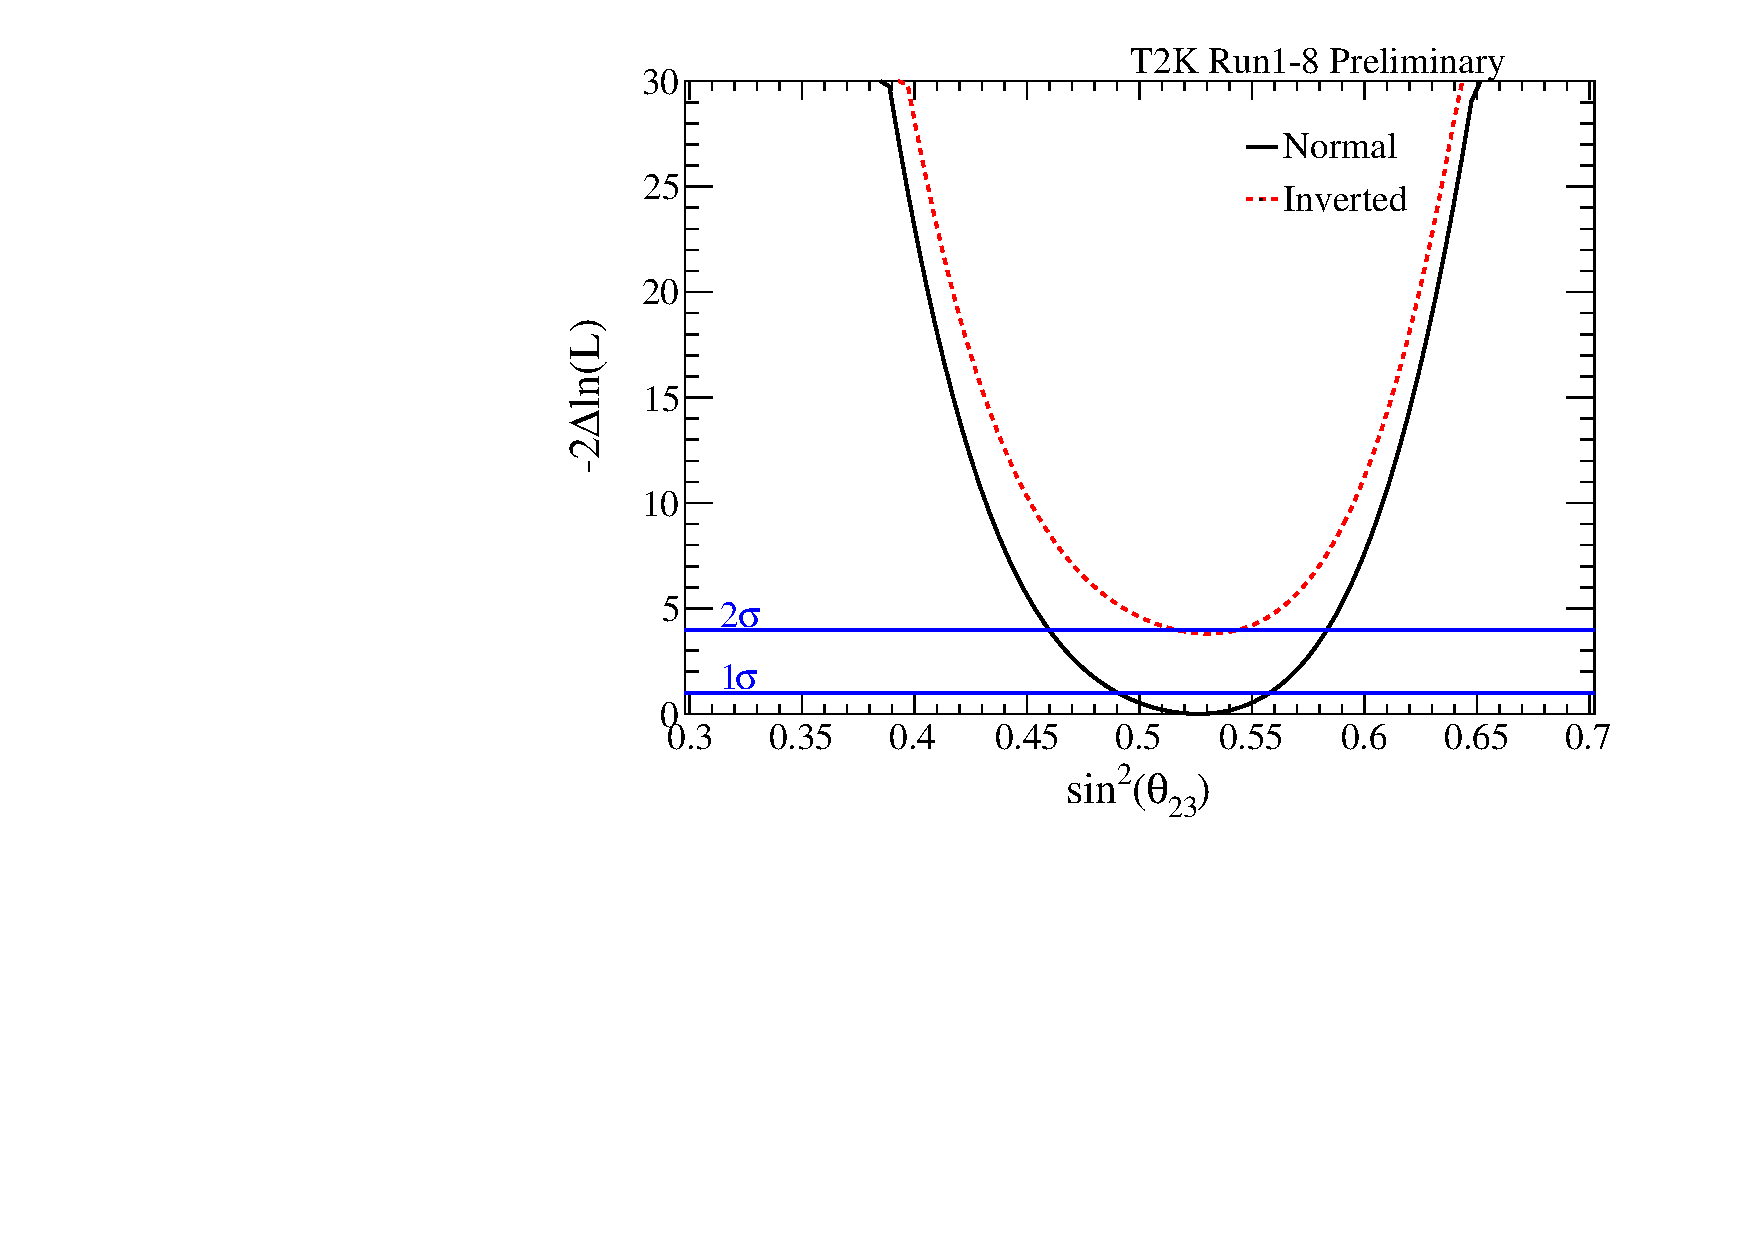
\includegraphics[width=0.9\textwidth]{data/reactor/2017b/mixing23_data_reactor_global}
		\caption{\ssqthtwothree with reactor constraint}
	\end{subfigure}
	\begin{subfigure}[b]{0.49\textwidth}
		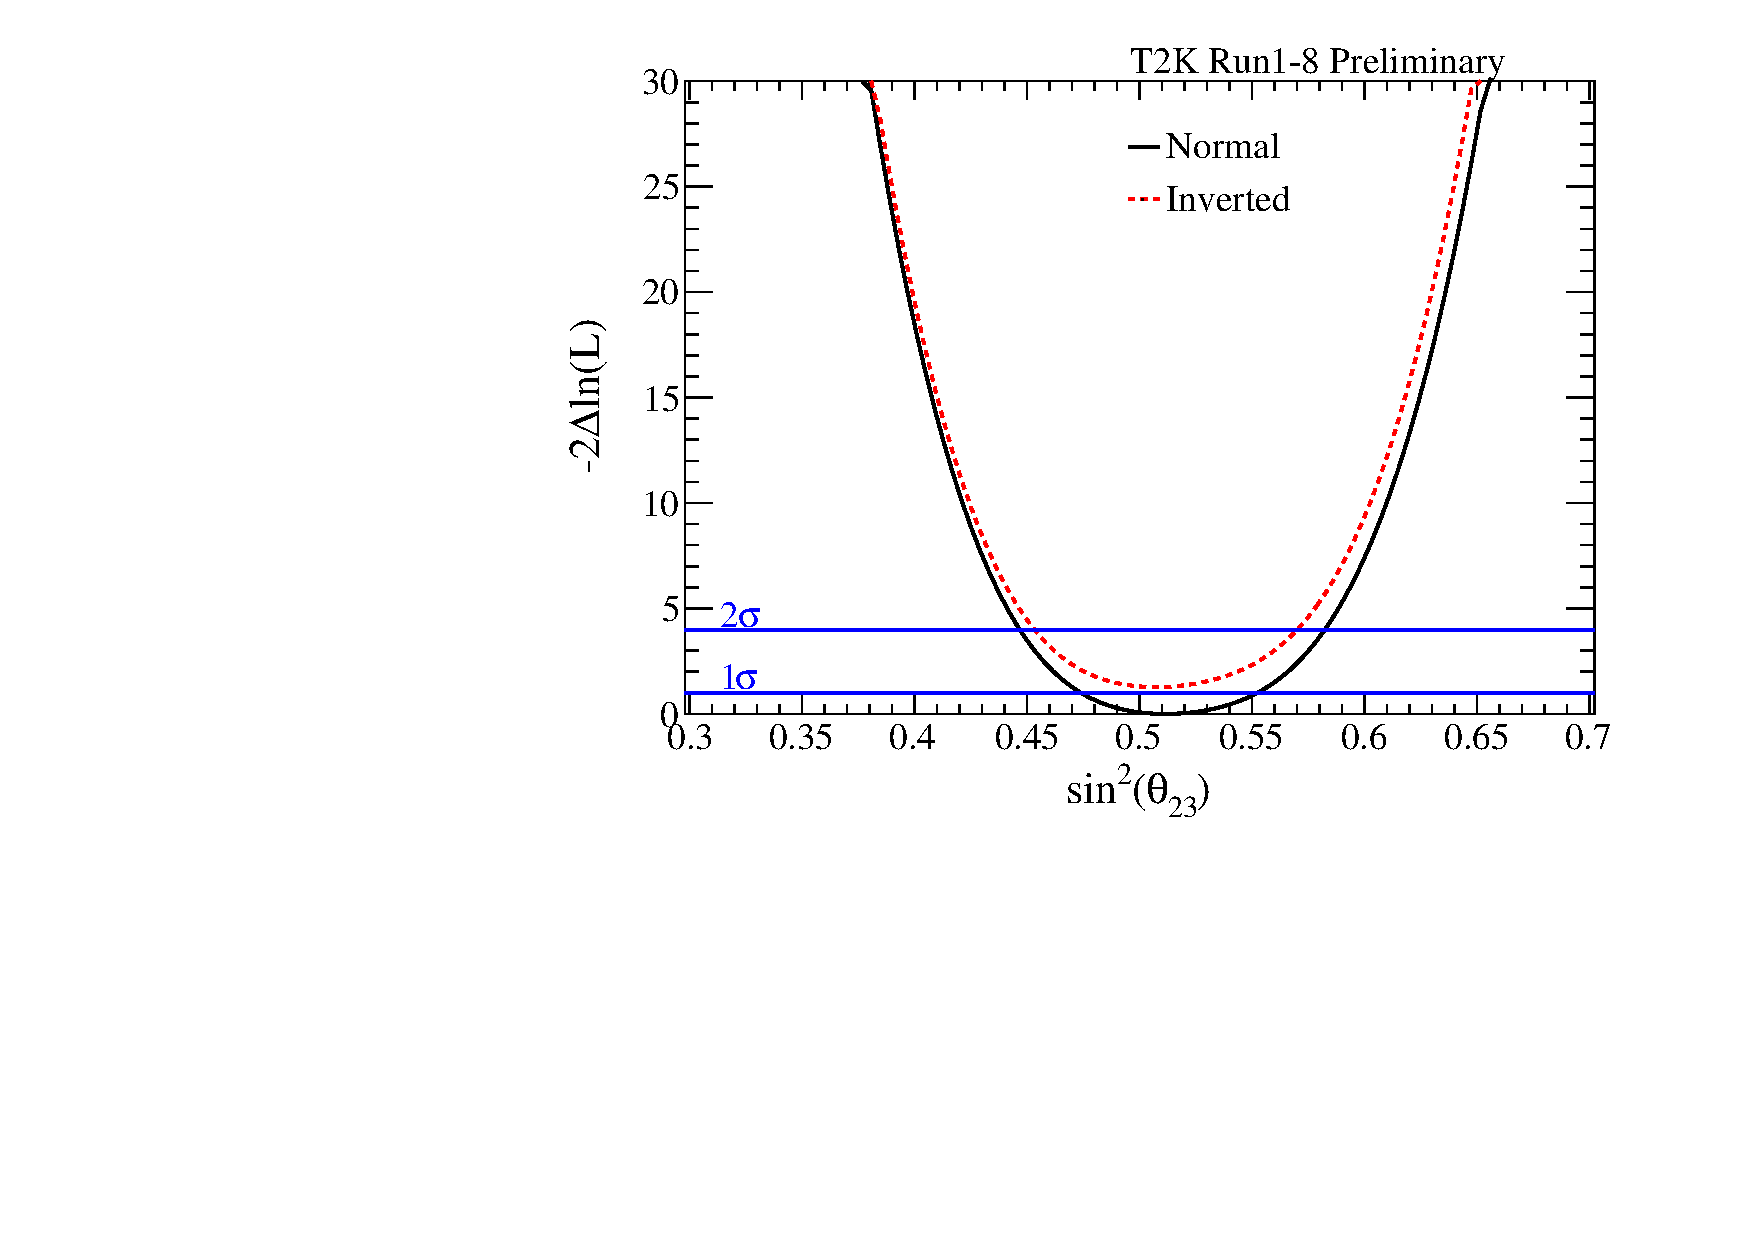
\includegraphics[width=0.9\textwidth]{data/t2k/2017b/mixing23_data_t2k_global}
		\caption{\ssqthtwothree T2K only}
	\end{subfigure}
	\caption {
		The expected $\Delta\chi^2$ distribution as a function of \ssqthtwothree with and without reactor constraint. The mass hierarchy is minimized, with normal and inverted hierarchy $\Delta\chi^2$ distributions shifted to the same global best-fit $\chi^2$ value, which is taken to be the minimum between normal and inverted hierarchy. All 5 samples were used to produce these fits.
	}
	\label{fig:th23_data_2017b}
\end{figure*}

\subsubsection{Results for \dmsq}

The result for \dmsq with reactor constraint and T2K only is shown in fig.~\ref{fig:dmsq23_data_2017b}.

\begin{figure*}[htb]
	\center
	\begin{subfigure}[b]{0.49\textwidth}
		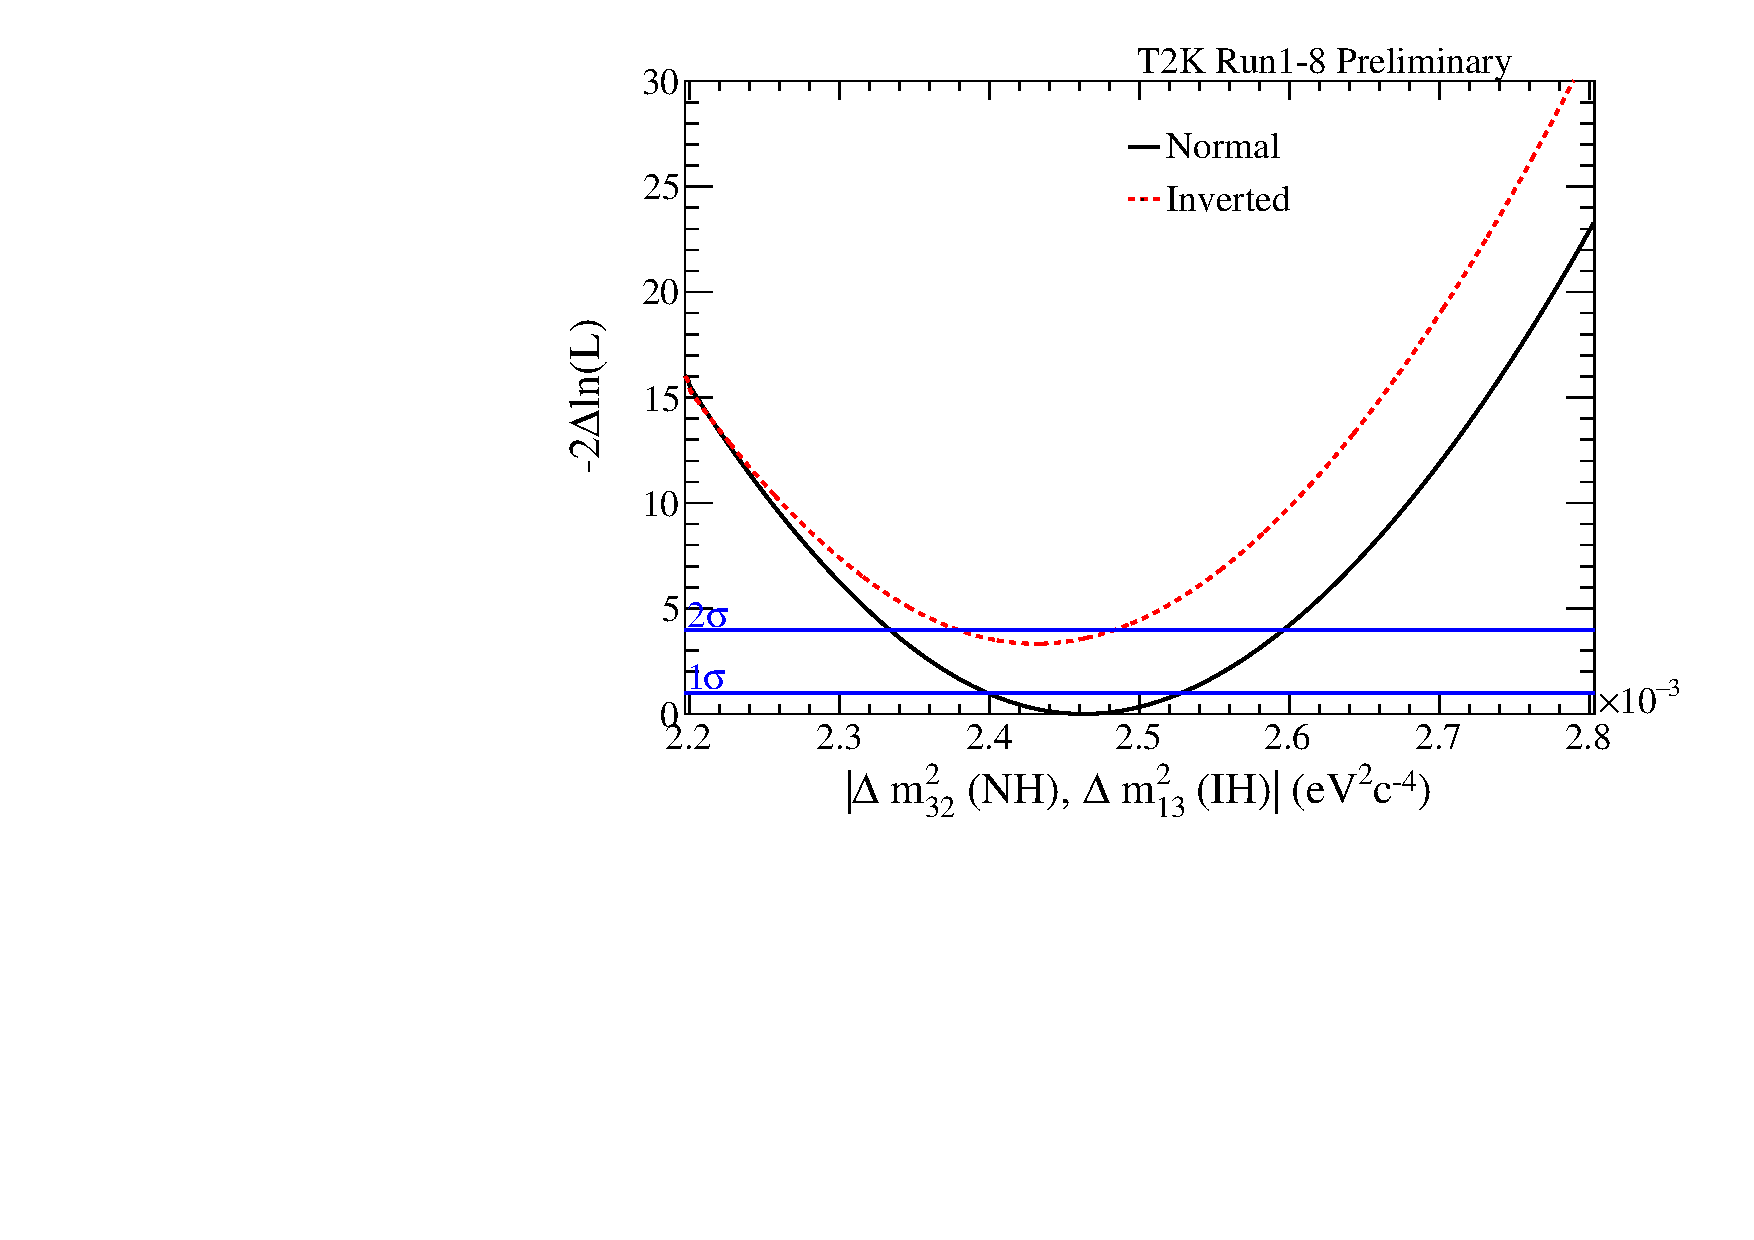
\includegraphics[width=0.9\textwidth]{data/reactor/2017b/dmsq23_data_reactor_global}
		\caption{\dmsq with reactor constraint}
	\end{subfigure}
	\begin{subfigure}[b]{0.49\textwidth}
		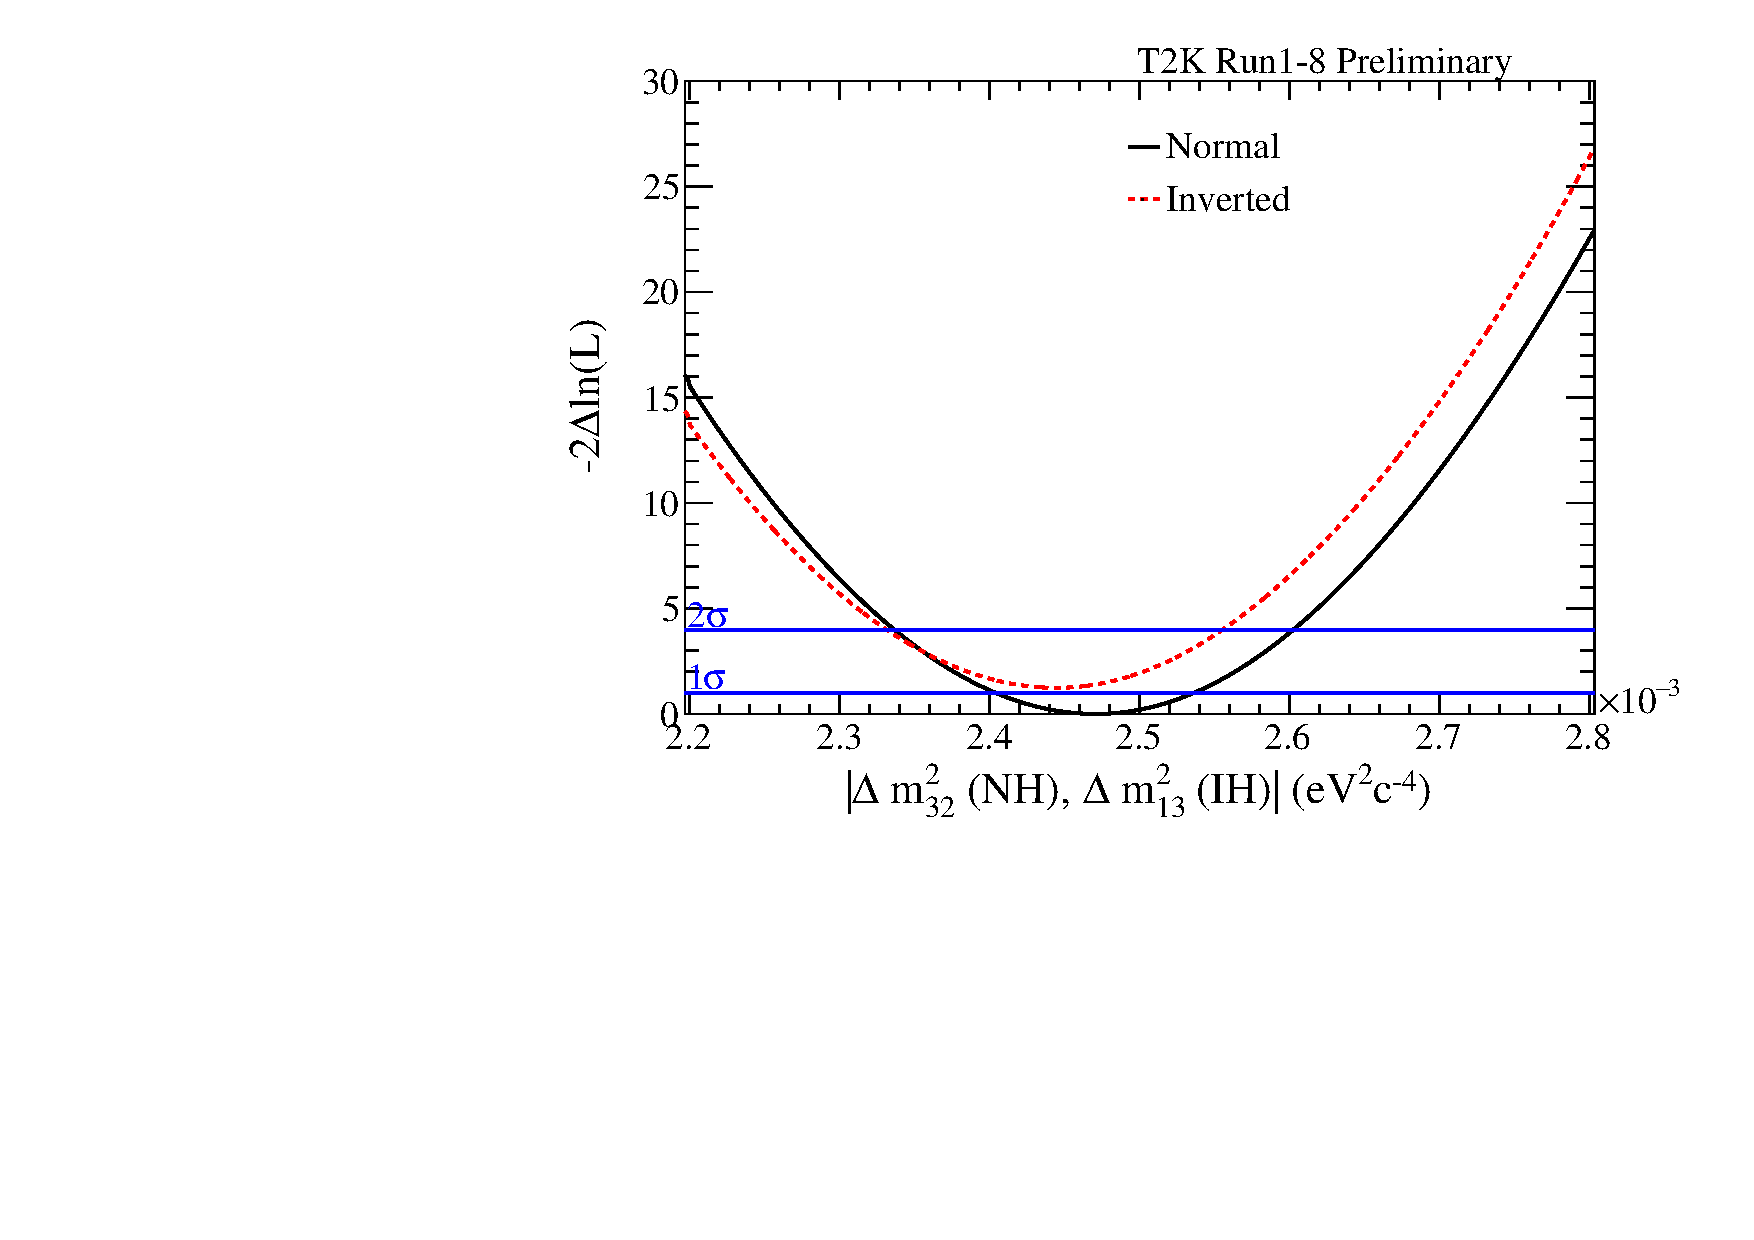
\includegraphics[width=0.9\textwidth]{data/t2k/2017b/dmsq23_data_t2k_global}
		\caption{\dmsq T2K only}
	\end{subfigure}
	\caption {
		The expected $\Delta\chi^2$ distribution as a function of \dmsq with and without reactor constraint. The mass hierarchy is minimized, with normal and inverted hierarchy $\Delta\chi^2$ distributions shifted to the same global best-fit $\chi^2$ value, which is taken to be the minimum between normal and inverted hierarchy. All 5 samples were used to produce these fits.
	}
	\label{fig:dmsq23_data_2017b}
\end{figure*}

\subsection {Feldman-Cousins simultaneous fit of \deltacp and mass hierarchy}
\label{sec:fc_significance_2017b}

This section presents the results of the Feldman-Cousins fit of \deltacp and mass hierarchy. Throws of oscillation parameters are made according to PDG 2016 best-fit values and errors for \ssqthonethree, \ssqthonetwo and \dmsqonetwo, whilst \ssqthtwothree and \dmsq are thrown according to the smeared likelihood distribution produced by an Asimov fit using the best-fit from data for these parameters. \deltacp is fixed at one of 9 evenly specified values on the range $\left[-\pi,\pi\right]$.

\subsubsection{Input oscillation parameters}
\label{sec:fc_significance:inputs_2017b}

The distributions of oscillation parameters (for normal hierarchy) are shown in \cref{fig:fc_input_dist_2017b}. The distributions of the atmospheric parameters are shown in \cref{fig:fc_input_disapp_2017b}.

\begin{figure*}[htb]
	\center
	\begin{subfigure}[b]{0.49\textwidth}
		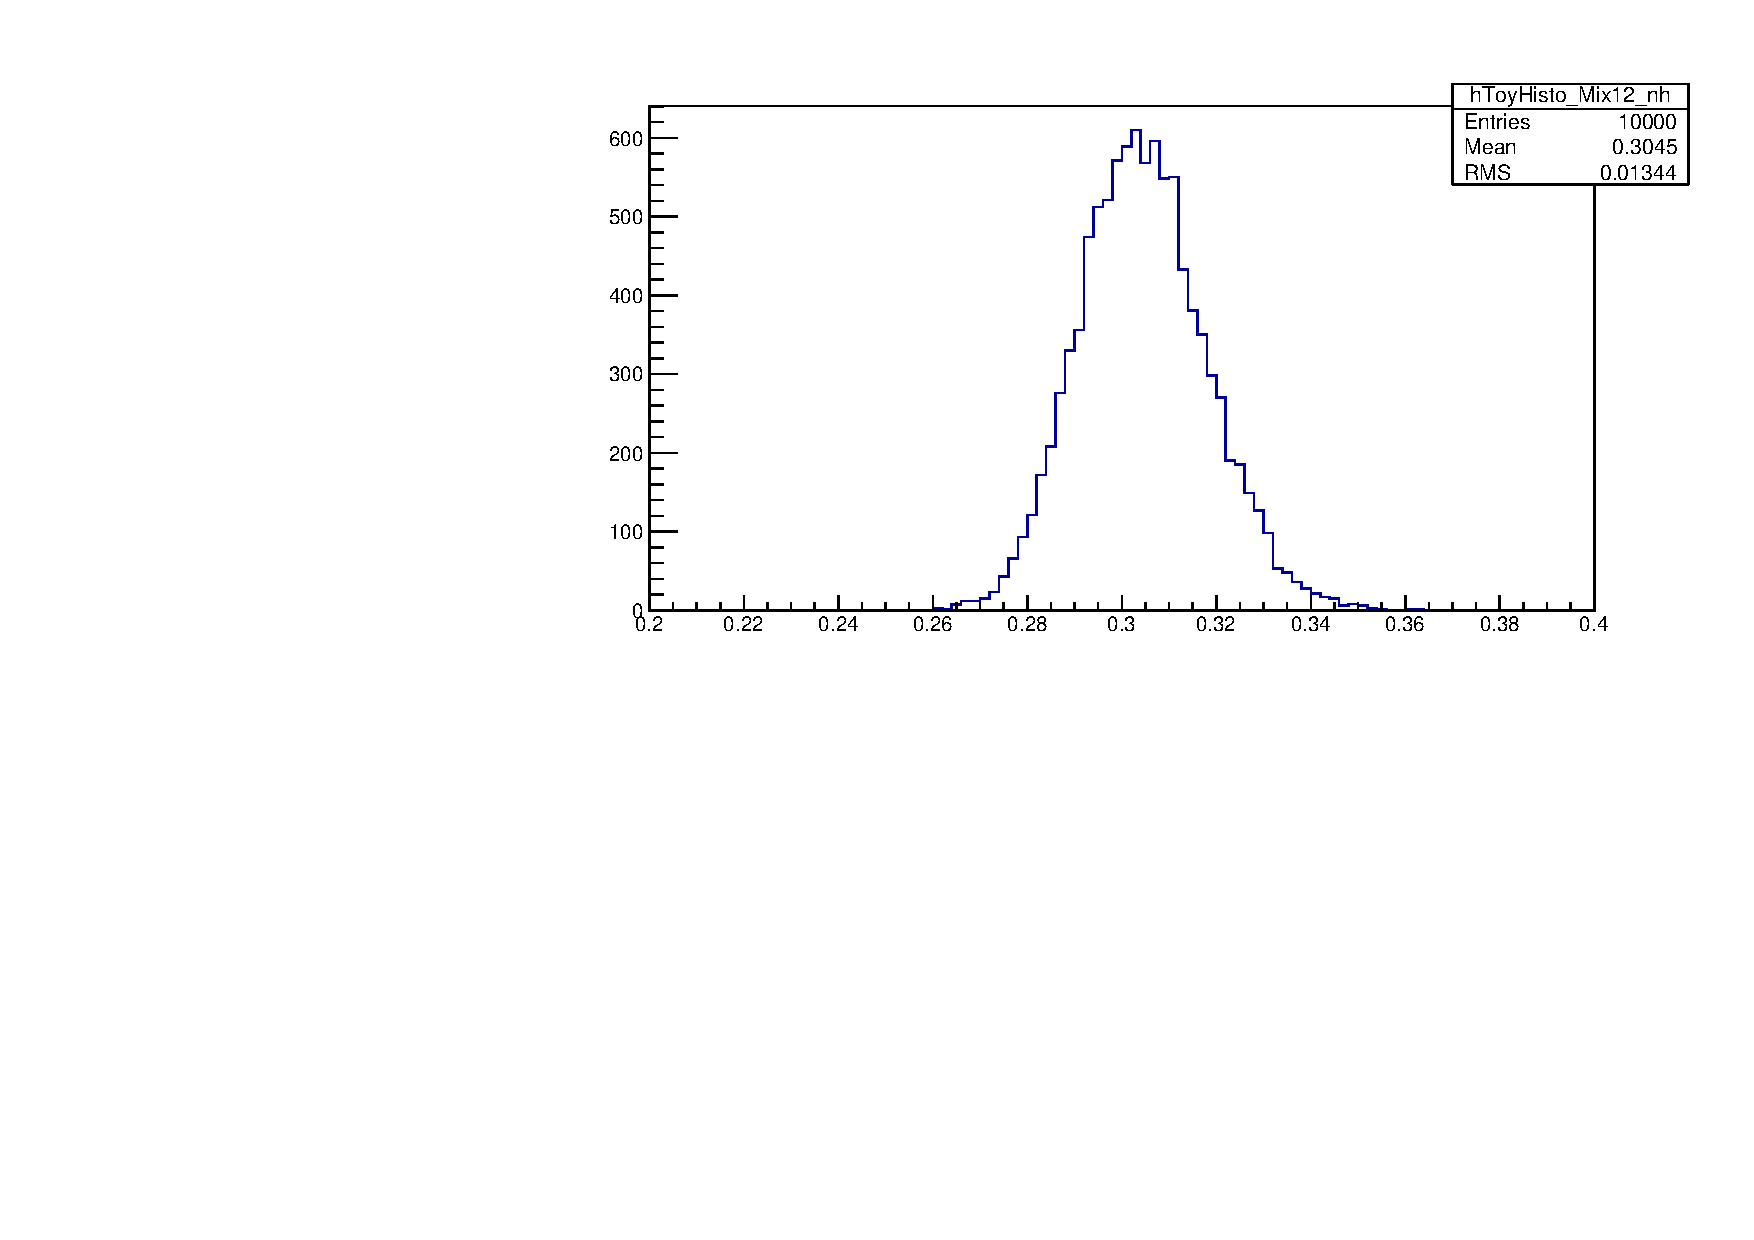
\includegraphics[width=0.9\textwidth]{data/fc/inputs/2017b/mixing12_in}
		\caption{\ssqthonetwo}
	\end{subfigure}
	\begin{subfigure}[b]{0.49\textwidth}
		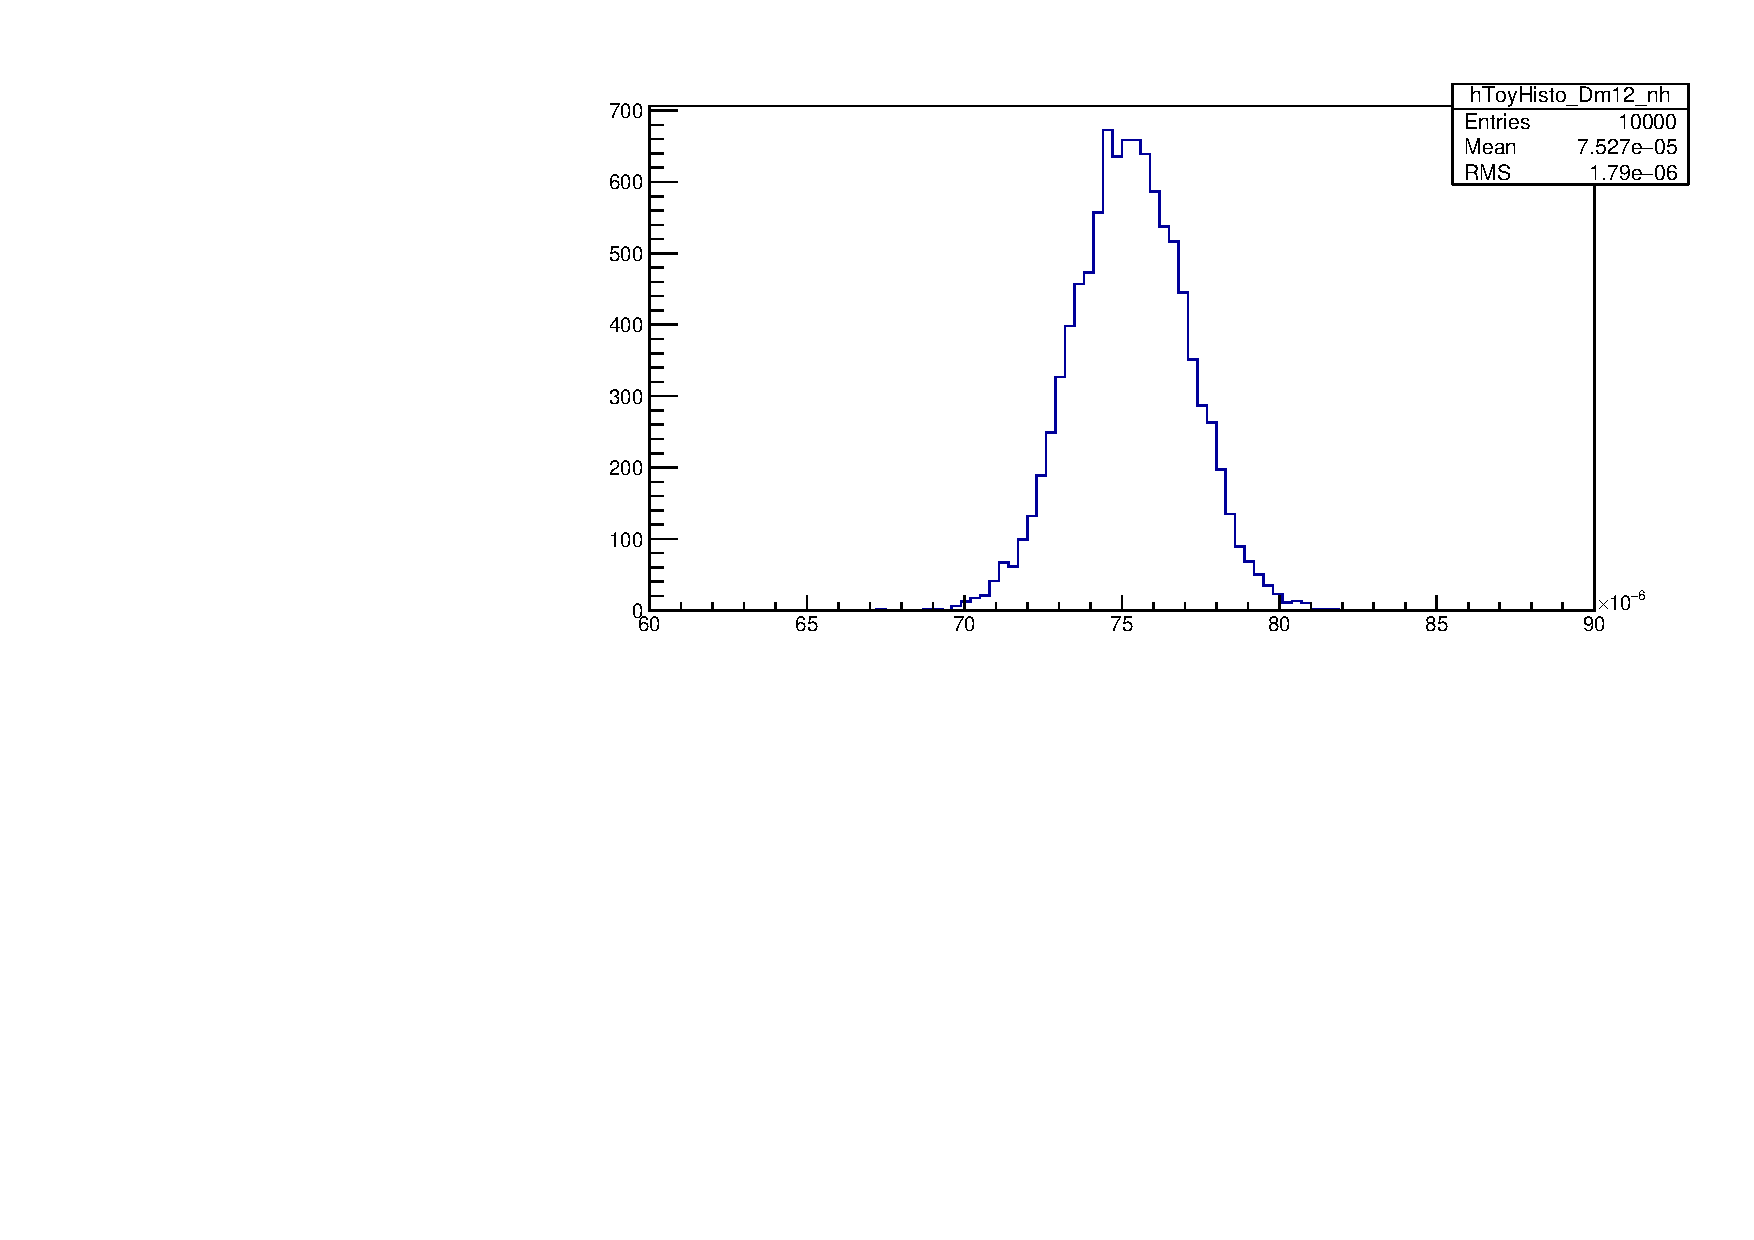
\includegraphics[width=0.9\textwidth]{data/fc/inputs/2017b/dmsq12_in}
		\caption{\dmsqonetwo}
	\end{subfigure}
	\begin{subfigure}[b]{0.49\textwidth}
		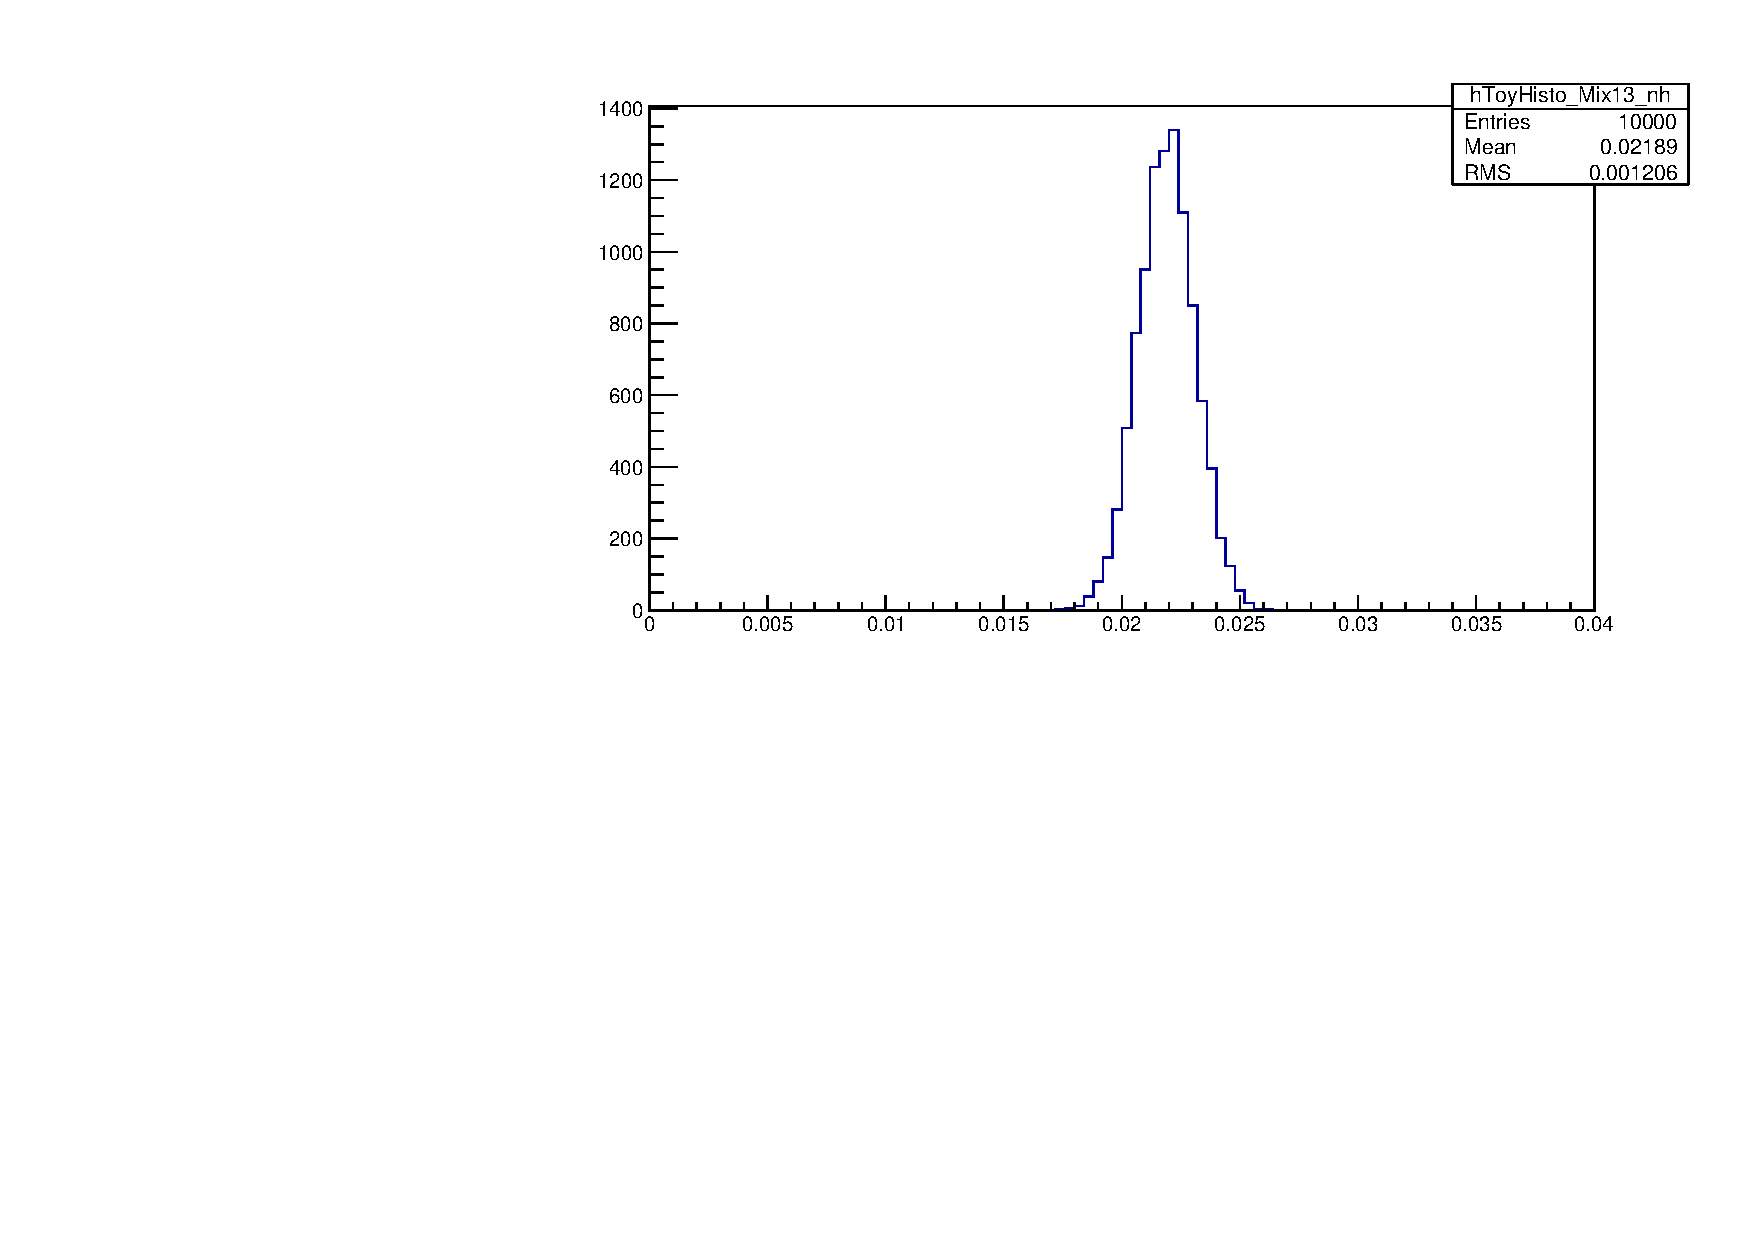
\includegraphics[width=0.9\textwidth]{data/fc/inputs/2017b/mixing13_in}
		\caption{\ssqthonethree}
	\end{subfigure}
	\caption {
		Distribution of oscillation parameter throws for Feldman-Cousins fits.
	}
	\label{fig:fc_input_dist_2017b}
\end{figure*}

\begin{figure*}[htb]
	\begin{subfigure}[b]{0.49\textwidth}
		\includegraphics[width=0.9\textwidth, page=2]{data/fc/inputs/2017b/disappearance_nh_likelihood}
		\caption{Normal hierarchy}
	\end{subfigure}
	\begin{subfigure}[b]{0.49\textwidth}
		\includegraphics[width=0.9\textwidth, page=2]{data/fc/inputs/2017b/disappearance_ih_likelihood}
		\caption{Inverted hierarchy}
	\end{subfigure}
	\caption {
		Likelihood surfaces for throws of the disappearance parameter.
	}
	\label{fig:fc_input_disapp_2017b}
\end{figure*}

\subsubsection{Feldman-Cousins critical values and confidence intervals}
\label{sec:fc_significance:intervals_2017b}

In \cref{fig:fc_interval_2017b} the confidence intervals obtained with the `Feldman-Cousins' method are shown for \deltacp and mass hierarchy with reactor constraint for the \RunPeriod data set. The critical values at 90\%, $2\sigma$ and $3\sigma$ CL are computed for both the mass hierarchies at the following true values of \deltacp; $-\pi$, $-3\pi/4$, $-\pi/2$, $-\pi/4$, 0, $+\pi/4$, $+\pi/2$, $+3\pi/4$, and $+\pi$. Inverted hierarchy is almost excluded at $2\sigma$, except for a small interval around $\delta_{CP} = -\pi/2$. Both $\delta_{CP} = 0$ and $\delta_{CP} = \pi$ are excluded at $2\sigma$. In \cref{tab:fc_interval_2017b} the $2\sigma$ CL intervals for \deltacp versus mass hierarchy, obtained with the Feldman-Cousins method, are shown. \color{blue}Comparison to p-theta critical values are shown in \cref{app:fc_compare}.\color{black}

\begin{figure*}[htb]
	\center
	\begin{subfigure}[b]{0.6\textwidth}
		\includegraphics[width=0.9\textwidth]{data/fc/2017b/FC_critical_values}
		\caption{\label{fig:fc_critval_2017b}Critical $\Delta\chi^2$ values}
	\end{subfigure}
	\begin{subfigure}[b]{0.49\textwidth}
		\includegraphics[width=0.9\textwidth]{data/fc/2017b/deltacp_FC_1sigma_CL}
		\caption{$1\sigma$ CL exclusion region}
	\end{subfigure}
	\begin{subfigure}[b]{0.49\textwidth}
		\includegraphics[width=0.9\textwidth]{data/fc/2017b/deltacp_FC_90_CL}
		\caption{90\% CL exclusion region}
	\end{subfigure}
	\begin{subfigure}[b]{0.49\textwidth}
		\includegraphics[width=0.9\textwidth]{data/fc/2017b/deltacp_FC_2sigma_CL}
		\caption{$2\sigma$ CL exclusion region}
	\end{subfigure}
	\caption {
$\Delta\chi^2$ critical values and confidence intervals for the measured $\Delta\chi^2$ distributions for \RunPeriod. Critical values obtained with the Feldman-Cousins method for \RunPeriod for 9 evenly spaced values on the range \( \left[-\pi,\pi\right] \). Critical values are shown for 1\( \sigma \), 2\( \sigma \) and 90\% CL for normal (solid lines) and inverted (dashed lines) hierarchies. At least \num{1e4} toy experiments are performed for each point. The three bands of lines show the \( \pm 1\sigma \) uncertainty on the critical values. Also shown are the measured \( \Delta \chi^2 \) distributions shifted with respect to the same global minium and the $1\sigma$, 90\% and $2\sigma$ exclusion regions for both mass hierarchies. 
	}
	\label{fig:fc_interval_2017b}
\end{figure*}

\begin{table}[htb]
	\centering
	\begin{tabular}{| c | c | c | c | c |}
\hline
Parameter & Reactor & CL & Normal hierarchy & Inverted hierarchy \\
\hline
\deltacp		& Yes & 90\% & $\left[ -2.815, -0.847 \right]$ & - \\
\deltacp		& Yes & $ 2\sigma $ & $\left[ -2.992, -0.592 \right]$ & $\left[ -1.808, -1.005 \right]$ \\
\hline
\end{tabular}

	\caption{
		The confidence intervals at 90\% CL and $2\sigma$ CL obtained with the Feldman-Cousins method for the \RunPeriod data set is shown for the measurement of \deltacp versus mass hierarchy.
	}
	\label{tab:fc_interval_2017b}
\end{table}

\subsubsection{$\delta_{CP} = -\pi/2$ - normal hierarchy}

In \cref{fig:brazilian_dcp_mpi2_2017b} the \RunPeriod data result for \deltacp versus mass hierarchy is compared to \color{blue}68.27\% and 95.45\% of toys from a $\Delta\chi^2$ distribution\color{black} corresponding to $\delta_{CP} = -\pi/2$ and (a) normal hierarchy and (b) inverted hierarchy. \color{blue}We see that more than 4.45\% ($2\sigma$ level) of toys provide a stronger constraint than the data contour for both normal and inverted hierarchy, consistent with the PMNS matrix\color{black}.

\color{blue}We also see an interesting feature near $\delta_{CP} = -\pi/2$ where the $\Delta\chi^2$ values have a wider distribution. This is due to the boundary at $\delta_{CP} = -\pi/2$ which causes a wider distribution when the parameter \deltacp would like to be pushed beyond the boundary in the fit.\color{black}

Finally from \cref{fig:brazilian_dcp_mpi2_2017b}(c) we see that $\delta_{CP} = 0$ and $\delta_{CP} = \pi$ are excluded at 90\% confidence level at between 40\% and 50\% (see \cref{tab:exclusion_prob_2017b}) of the toy experiments and excluded at $2\sigma$ confidence level in between 25\% and 35\% of the toy experiments, with $\delta_{CP} = \pi$ excluded in slightly fewer toy experiments in each case.

\begin{figure*}[htb]
	\center
	\begin{subfigure}[b]{0.49\textwidth}
		\includegraphics[width=0.9\textwidth]{comparison/2017b/dcp_run18_react_Data_braz_nh}
		\caption{Normal hierarchy}
	\end{subfigure}
	\begin{subfigure}[b]{0.49\textwidth}
		\includegraphics[width=0.9\textwidth]{comparison/2017b/dcp_run18_react_Data_braz_ih}
		\caption{Inverted hierarchy}
	\end{subfigure}
	\begin{subfigure}[b]{0.49\textwidth}
		\includegraphics[width=0.9\textwidth]{comparison/2017b/dcp_run18_react_Data_prob_chisq}
		\caption{Data \(\Delta \chi^2\) probability }
	\end{subfigure}
	\caption {
		The distribution of $\Delta\chi^2$ vs \deltacp obtained with \num{1e4} toy experiments generated with $\delta_{CP} = -\pi/2$ and normal hierarchy is shown. The $\Delta\chi^2$ distributions obtained by fixing the mass hierarchy to normal (left) and inverted (right) are shown, along with the $\Delta\chi^2$ values corresponding to 68.27\% and 95.45\% of the toy experiments and the average $\Delta\chi^2$ values from all experiments. Also shown are the fractions of toys which exclude each value of \deltacp to 90\% and $2\sigma$ using the Feldman-Cousins corrected critical values (bottom).
	}
	\label{fig:brazilian_dcp_mpi2_2017b}
\end{figure*}

\begin{table}[htb]
	\centering
	\begin{tabular}{| c | c | c | c |}
\hline
\deltacp & Hierarchy & 90\% & $2\sigma$ \\
\hline
0		& NH & 0.474 & 0.332 \\
$\pi$	& NH & 0.414 & 0.279 \\
0		& IH & 0.803 & 0.708 \\
$\pi$	& IH & 0.796 & 0.693 \\
\hline
\end{tabular}

	\caption{
		The fraction of toy experiments for which $\delta_{CP} = 0, \pi$ and normal and inverted hierarchy are excluded at 90\% and $2\sigma$ CL is shown. 10k toy experiments are used.
	}
	\label{tab:exclusion_prob_2017b}
\end{table}

\clearpage

\subsection{Comparison to 2017 results}
\label{sec:results:comparison}

This section presents comparisons of the updated fits with the 2017 fits described in \cref{sec:results} for the case of reactor fits (except in the case of \ssqthonethree, which does not apply the reactor constraint).

\subsubsection{Results for \appearance}
In \cref{fig:ssqth13_vs_dcp_data_compare} the result for \appearance with reactor constraint.

\begin{figure*}[htb]
	\center
	\begin{subfigure}[b]{0.49\textwidth}
		\includegraphics[width=0.9\textwidth]{data/reactor/2017b/comparisons/mixing13_deltacp_data_reactor_nh}
		\caption{\appearance NH}
	\end{subfigure}
	\begin{subfigure}[b]{0.49\textwidth}
		\includegraphics[width=0.9\textwidth]{data/reactor/2017b/comparisons/mixing13_deltacp_data_reactor_ih}
		\caption{\appearance IH}
	\end{subfigure}
	\caption {
		Contours at 68\% and 90\% CL for \appearance with reactor constraint. Normal and inverted hierarchy contours are independent. All 5 samples were used to produce these fits.
	}
	\label{fig:ssqth13_vs_dcp_data_compare}
\end{figure*}

\subsubsection{Results for \disappearance}

The result for \disappearance with reactor constraint is shown in fig.~\ref{fig:ssqth23_vs_dmsq23_data_compare}.

\begin{figure*}[htb]
	\center
	\begin{subfigure}[b]{0.49\textwidth}
		\includegraphics[width=0.9\textwidth]{data/reactor/2017b/comparisons/mixing23_dmsq23_data_reactor_nh}
		\caption{\disappearance NH}
	\end{subfigure}
	\begin{subfigure}[b]{0.49\textwidth}
		\includegraphics[width=0.9\textwidth]{data/reactor/2017b/comparisons/mixing23_dmsq23_data_reactor_ih}
		\caption{\disappearance IH}
	\end{subfigure}
	\caption {
		Contours at 68\% and 90\% CL for \disappearance with reactor constraint. Normal and inverted hierarchy contours are independent. All 5 samples were used to produce these fits.
	}
	\label{fig:ssqth23_vs_dmsq23_data_compare}
\end{figure*}

\clearpage

\subsubsection{Results for \deltacp}

The result for \deltacp with reactor constraint is shown in fig.~\ref{fig:dcp_data_compare}.

\begin{figure*}[htb]
	\center
	\begin{subfigure}[b]{0.49\textwidth}
		\includegraphics[width=0.9\textwidth]{data/reactor/2017b/comparisons/deltacp_data_reactor_nh}
		\caption{\deltacp NH}
	\end{subfigure}
	\begin{subfigure}[b]{0.49\textwidth}
		\includegraphics[width=0.9\textwidth]{data/reactor/2017b/comparisons/deltacp_data_reactor_ih}
		\caption{\deltacp IH}
	\end{subfigure}
	\caption {
		The expected $\Delta\chi^2$ distribution as a function of \deltacp with reactor constraint. The mass hierarchy is minimized, with normal and inverted hierarchy $\Delta\chi^2$ distributions shifted to the same global best-fit $\chi^2$ value, which is taken to be the minimum between normal and inverted hierarchy. All 5 samples were used to produce these fits.
	}
	\label{fig:dcp_data_compare}
\end{figure*}

\subsubsection{Results for \ssqthonethree}

The result for \ssqthonethree (without reactor constraint) is shown in fig.~\ref{fig:th13_data_compare}.

\begin{figure*}[htb]
	\center
	\begin{subfigure}[b]{0.49\textwidth}
		\includegraphics[width=0.9\textwidth]{data/t2k/2017b/comparisons/mixing13_data_t2k_nh}
		\caption{\ssqthonethree NH}
	\end{subfigure}
	\begin{subfigure}[b]{0.49\textwidth}
		\includegraphics[width=0.9\textwidth]{data/t2k/2017b/comparisons/mixing13_data_t2k_ih}
		\caption{\ssqthonethree IH}
	\end{subfigure}
	\caption {
		The expected $\Delta\chi^2$ distribution as a function of \ssqthonethree without reactor constraint. The mass hierarchy is minimized, with normal and inverted hierarchy $\Delta\chi^2$ distributions shifted to the same global best-fit $\chi^2$ value, which is taken to be the minimum between normal and inverted hierarchy. All 5 samples were used to produce these fits.
	}
	\label{fig:th13_data_compare}
\end{figure*}

\clearpage

\subsubsection{Results for \ssqthtwothree}

The result for \ssqthtwothree with reactor constraint is shown in fig.~\ref{fig:th23_data_compare}.

\begin{figure*}[htb]
	\center
	\begin{subfigure}[b]{0.49\textwidth}
		\includegraphics[width=0.9\textwidth]{data/reactor/2017b/comparisons/mixing23_data_reactor_nh}
		\caption{\ssqthtwothree NH}
	\end{subfigure}
	\begin{subfigure}[b]{0.49\textwidth}
		\includegraphics[width=0.9\textwidth]{data/reactor/2017b/comparisons/mixing23_data_reactor_ih}
		\caption{\ssqthtwothree IH}
	\end{subfigure}
	\caption {
		The expected $\Delta\chi^2$ distribution as a function of \ssqthtwothree with reactor constraint. The mass hierarchy is minimized, with normal and inverted hierarchy $\Delta\chi^2$ distributions shifted to the same global best-fit $\chi^2$ value, which is taken to be the minimum between normal and inverted hierarchy. All 5 samples were used to produce these fits.
	}
	\label{fig:th23_data_compare}
\end{figure*}

\subsubsection{Results for \dmsq}

The result for \dmsq with reactor constraint is shown in fig.~\ref{fig:dmsq23_data_compare}.

\begin{figure*}[htb]
	\center
	\begin{subfigure}[b]{0.49\textwidth}
		\includegraphics[width=0.9\textwidth]{data/reactor/2017b/comparisons/dmsq23_data_reactor_nh}
		\caption{\dmsq NH}
	\end{subfigure}
	\begin{subfigure}[b]{0.49\textwidth}
		\includegraphics[width=0.9\textwidth]{data/reactor/2017b/comparisons/dmsq23_data_reactor_ih}
		\caption{\dmsq IH}
	\end{subfigure}
	\caption {
		The expected $\Delta\chi^2$ distribution as a function of \dmsq with reactor constraint. The mass hierarchy is minimized, with normal and inverted hierarchy $\Delta\chi^2$ distributions shifted to the same global best-fit $\chi^2$ value, which is taken to be the minimum between normal and inverted hierarchy. All 5 samples were used to produce these fits.
	}
	\label{fig:dmsq23_data_compare}
\end{figure*}

\subsection {Discussion of the \RunPeriod data fit results}
\label{sec:results:discussion_2017b}

It can be seen from section \cref{sec:results:comparison} that the majority of fits show little change between the 2017 and updated analyses for fits of \ssqthonethree, \ssqthtwothree and \deltacp. The best-fit values show changes of no more than a single bin in the fit parameter; this being most evident in the normal hierarchy \appearance fit, where the binning is coarser. The contours for the \appearance fit are almost identical. A moderate inflation of the T2K-only \ssqthonethree contour in normal hierarchy can be seen. \color{blue}A possible explanation of the asymmetry in the inflation of this contour is that as the value of \ssqthonethree increases a larger combination of values of other oscillation parameters can produce equivalent spectra; the addition of the Eb parameter then provides additional freedom in this respect and thereby weakens the fit in this region. The effect diminishes for smaller values of \ssqthonethree as there is less of an appearance signal for Eb to act upon\color{black}. Modest changes in the \deltacp contours are evident, with slightly less extreme values of $\Delta\chi^2$ around the peak near $\delta_{CP}=\pi/2$, but this does not alter the rejection of CP conservation at $2\sigma$, as demonstrated in \cref{sec:fc_significance:intervals_2017b}.

Differences are evident in the fits of the atmospheric parameters, particularly \dmsq. The addition of the Eb parameter and \dmsq smearing has inflated the contours, most notably in the \dmsq parameter, as expected. The best-fit point is little changed in normal hierarchy (again being most evident in the coarser-binned 2D fit), and a small shift in \dmsq is observed in both 2D and 1D fits in inverted hierarchy. The 1D fits of \ssqthtwothree show slight inflation of the contours, with the inflation clearly evident in the 1D fits of \dmsq.

\clearpage

%%% Local Variables:
%%% mode: latex
%%% TeX-master: "../TN327"
%%% End:

\clearpage

% --------------------------------------------------------------------------------------------

\section{Summary}
\label{sec:summary}

In this technical note, we have presented the results of the 3-flavour $\bar{\nu}/\nu$ joint analysis performed by the {\em VALOR} group, on the combined \RunPeriod data set. The goal of the analysis was to search for CP violation in the leptonic sector and determine limits on \deltacp as well as measure all the other oscillation parameters to which T2K is sensitive: \ssqthonethree, \ssqthtwothree, \dmsqtwothree (\dmsqonethree) and partially mass hierarchy, to which T2K has little sensitivity.

This analysis predicts
\NskOscExpectationNumuRunOneEight{} $\pm$ \NskOscExpectationNumuErrorRunOneEight{} (syst) for neutrino $\mu$-like, \NskOscExpectationNumuBarRunOneEight{} $\pm$ \NskOscExpectationNumuBarErrorRunOneEight{} (syst) for antineutrino $\mu$-like, \NskOscExpectationNueRunOneEight{} $\pm$ \NskOscExpectationNueErrorRunOneEight{} (syst) for neutrino $e$-like, \NskOscExpectationNueBarRunOneEight{} $\pm$ \NskOscExpectationNueBarErrorRunOneEight{} (syst) for antineutrino $e$-like and \NskOscExpectationNueCConepiRunOneEight{} $\pm$ \NskOscExpectationNueCConepiErrorRunOneEight{} (syst) for neutrino \nueCConepi{} events in Super K and observes respectively \NskObservedNumuRunOneEight{} for neutrino $\mu$-like, \NskObservedNumuBarRunOneEight{}  for antineutrino $\mu$-like, \NskObservedNueRunOneEight{}  for neutrino $e$-like, \NskObservedNueBarRunOneEight{}  for antineutrino $e$-like and \NskObservedNueCConepiRunOneEight{} for neutrino \nueCConepi{}. 

The $\bar{\nu}/\nu$ analysis was performed in a framework of 3-flavour oscillations including matter effects in constant-density matter. The observed reconstructed energy spectrum of single $\mu$-like ring events and reconstructed energy versus lepton angle of single $e$-like ring events in addition to $e$-like events with an additional decay electron were used to compute the confidence intervals. All \NSyst{} systematic parameters as well as the oscillation parameters which were not parameters of interest considered in this analysis were marginalised.

From the fit of the \RunPeriod data we can see that the favoured value of \deltacp is \BestFitDeltacpwRCb, close to $-\pi/2$. The Feldman-Cousins method is used to construct confidence intervals with neither over or under coverage from which the significance to exclude the hypothesis of CP conservation is greater than 2 standard deviations. 

\clearpage

%%% Local Variables:
%%% mode: latex
%%% TeX-master: "../TN327"
%%% End:


% References
\clearpage
%
% References
%

% TODO: Find out how to automatically not display unused references

\begin{thebibliography}{9}

\bibitem{OurRun16AntiNueBarAppearanceAnalysis3Flavour}
C.Andreopoulos et al.,
$\nueb$ Appearance Analysis with the 3-Flavour Joint Fit Framework for T2K \TotalPotNuRunOneSix-POT Neutrino \TotalPotNuBarRunOneSix-POT Anti-Neutrino
T2K-TN-296,\\
http://www.t2k.org/docs/technotes/296

\bibitem{OurRun18CC1piJointAnalysis3Flavour}
C.Andreopoulos et al.,
T2K Neutrino and Anti-Neutrino 3-Flavour Joint Analysis of Run 1-9c (\TotalPotNuRunOneNineC-POT $\nu$ \TotalPotNuBarRunOneNineC-POT $\bar{\nu}$) data sets
T2K-TN-327,\\
http://www.t2k.org/docs/technotes/327	

\bibitem{OurRun19JointAnalysis3Flavour}
C.Andreopoulos et al.,
T2K Neutrino and Anti-Neutrino 3-Flavour Joint Analysis of Run 1-9c (\TotalPotNuRunOneNine-POT $\nu$ \TotalPotNuBarRunOneNine-POT $\bar{\nu}$) data sets - Statistical Update
T2K-TN-360,\\
https://t2k.org/docs/technotes/360/run19d/statistical-update

\bibitem{pdg_2014}
K.A. Olive et al. (Particle Data Group 2014 with 2015 update), 
Chin. Phys. C, 38, 090001

\bibitem{pdg_2018}
M. Tanabashi et al. (Particle Data Group), 
Phys. Rev. D 98, 030001 (2018)

t2k neutrino\bibitem{T2KLongPaper}
T2K Collaboration (K.Abe et al.),
Measurement of neutrino oscillation in appearance and disappearance channels by the T2K experiment with 
6.6$\times$10$^{20}$ protons on target 
http://www.t2k.org/comm/pubboard/JournalPapers/oa2014prd/draft3

\bibitem{fiTQunAlgo}
S. Berkman, P. de Perio, A. Konaka, A. Missert, H. Tanaka, S. Tobayama, M. J. Wilking, E. D. Zimmerman
fiTQun: A New Reconstruction Algorithm for Super-K
http://www.t2k.org/docs/technotes/146

\bibitem{PthetaR19cNuebarAppearance}
T.Koga, S.Bienstock, C.Bronner and B.Quilain,
Updated p-theta $\nueb$ appearance search using the T2K RUN1-9 data set,\\
http://www.t2k.org/docs/technotes/353

\bibitem{JeffreysScale}
H. Jeffreys
The Theory of Probability
OUP Oxford
1998

\bibitem{MaCH3NuebarAppearance2015}
A. Kaboth, K. Duffy, R Calland, and D Payne
Analysis of $\nueb$ Appearance using MCMC
T2K-TN-247
http://www.t2k.org/docs/technotes/247 

\bibitem{Asimov} 
G.Cowan, K.Cranmer, E.Gross, O.Vitells,
"Asymptotic formulae for likelihood-based tests of new physics"
arXiv:1007.1727v2

\bibitem{WilksTheorem}
S. Wilks,
The Large-Sample Distribution of the Likelihood Ratio for Testing Composite Hypotheses,
Ann. Math. Statist., 03, 1, 60-62,
https://doi.org/10.1214/aoms/1177732360

\bibitem{Grubbs}
F. Grubbs,
Sample Criteria for Testing Outlying Observations,
Ann. Math. Statist., 03, 1, 27-58,
https://doi.org/10.1214/aoms/1177729885

\bibitem{flux_tuning_Run1-9d}
T. Vladisavljevic,
Full Run 9 T2K Flux Release of  Run 9d (2018/3/9 – 2018/5/31),
https://t2k.org/beam/NuFlux/FluxRelease/13arelease/13av3-tuned-fluxes-for-runs-1-9d-slides

\bibitem{nuebarapp_valor_plenary_run1-9c}
F. Bench,
$\nueb$ Appearance Analysis,
https://t2k.org/meet/collab/201805/talks/fripm/nuebar

\end{thebibliography}



%%% Local Variables:
%%% mode: latex
%%% TeX-master: "../TN327"
%%% End:


%Appendices
\clearpage
\begin{appendices}
	\crefalias{section}{appsec}
	\section{Fitter details}
\label{app:details}

\subsection {Spectra prediction methodology}
\label{app:details:spectra_methodology}

In this analysis a comparison of the reconstructed energy ($E_{r}$) and reconstructed lepton angle ($\theta$) spectrum of single ring events, including the \nueCConepi{}-like sample, observed at Super-K with the predicted spectrum is used to build the test statistic to quote confidence intervals for neutrino oscillation parameters. For $\mu$-like samples the templates are built as a function of the reconstructed neutrino energy, as in previous analyses, and a single $\theta$ bin is used. The predicted number $N_{SK;r,\theta}$ of single ring events in the $r$-th and $\theta$-th bin is computed for each selected sample as follows:

\begin{equation}
\displaystyle
  N_{SK;r,\theta} = 
    \sum_{m} \sum_{t} \sum_{r\prime}
    	%\beta \cdot
        P_{m;t} \cdot
        T_{r;r\prime;f_{E; r}^{SK}} \cdot
        S_{m;t;r\prime,\theta;\vec{f}} \cdot
        N_{SK;m;r\prime,\theta;t}^{MC} 
         \label{eq:far_prediction}
\end{equation}

In \ref{eq:far_prediction}, $N_{SK;m;r\prime,\theta;t}^{MC}$ is the input Super-K Monte Carlo (MC) template containing the number of events in the single ring MC sample with true reaction mode $m$ in the true energy bin t, the reconstructed energy bin $r\prime$ and reconstructed lepton angle bin $\theta$. $S_{m;t;r\prime,\theta;\vec{f}}$ is an overall, multiplicative, systematic error factor depending on a vector of nuisance (systematic) parameters $\vec{f}$, which is function of the reaction mode $m$, the true energy bin $t$, the reconstructed energy bin $r\prime$, and the reconstructed lepton angle bin $\theta$. $T_{r;r\prime;f_{E; r}^{SK}}$ is a transfer function describing the migration of events between the reconstructed energy bins $r$ and $r\prime$ due to uncertainty in the Super-K reconstructed energy scale, expressed here in terms of the nuisance parameter $f_{E; r}^{SK}$. Finally, $P_{m;t}$ is the 3-flavour oscillation probability applied to the true energy
bin \(t\) of the Super-K MC template which corresponds to mode $m$; application of the term $P_{m;t}$ is discussed in \ref{app:details:applying_oscillations}.
\subsection {Construction of the nominal Super-K Monte Carlo templates}
\label{app:details:mc_templates}

The nominal Super-K single ring and \nueCConepi{} MC analysis templates $N_{SK;m;r\prime,\theta;t}^{MC}$ are constructed by applying the single $e$-like ring selection cuts, the \nueCConepi{} selection cuts, or the single $\mu$-like ring selection cuts to the official Super-K MC samples \cite{Superk_run8}. The calculation of the normalisation of each MC sample is described in \cref{app:details:mc_templates:normalization}. The list of MC templates used in this analysis is shown in \cref{app:details:mc_templates:template_list}, while the true and reconstructed energy as well as the reconstructed lepton angle binning of the templates are discussed in \cref{app:details:mc_templates:template_binning}.

\subsubsection {Normalisation of Monte Carlo samples}
\label{app:details:mc_templates:normalization}

The normalisation (integrated exposure in terms of POT) of each event sample is calculated from the number of events with a MC truth interaction vertex within the 22.5 kt fiducial volume.

\begin{equation}
\displaystyle
  N = \int  dS dI dE \cdot
            \frac{d^{3}\Phi_{SK}}{dS dI dE_{\nu}} \cdot
            \sigma_{H_{2}O} \cdot
            \frac{N_{A}}{A} \cdot \rho \cdot L 
\end{equation}
where $d^{3}\Phi_{SK}$/$dS dI dE$ is the number of flux particles for the given neutrino species per neutrino energy bin $dE_{\nu}$, per unit area $dS$ and per POT, $\sigma_{H_{2}O}$ is the total interaction cross section on water for the given neutrino species, $I$ is the beam exposure in terms of POT, $N_{A}$ is  Avogadro's number, $A$ is the mass number for water, $\rho$ is the water density and $L$ is the neutrino path length in the water volume.

The Super-K MC samples are normalised to the \RunPeriod POT. Assuming that all the MC files are used, each sample is first normalised to 10$^{21}$ POT by weighting it with the ratio of the number of events per 22.5 kt per $10^{21}$ POT to the number of generated events in the true fiducial volume in all the available MC. Then each sample is normalised to \TotalPotNuRunOneEight{} POT for neutrino and \TotalPotNuBarRunOneEight{} for antineutrino mode, by weighting the result respectively by \TotalPotPerTwentyOneNu{} and \TotalPotPerTwentyOneNuBar{} (the \RunPeriod POT in units of $10^{21}$ POT). 

\subsubsection {List of Monte Carlo templates}
\label{app:details:mc_templates:template_list}

For each Super-K MC sample, a number of different MC templates is constructed corresponding to different true reaction modes. The template number depends on the type of oscillation analysis and the specific systematic parameters considered in the analysis. \NMCTemplate{} are used for the current analysis, these are the same templates as in our 2016 analysis \cite{OurRun17cCC1piJointAnalysis3Flavour}. In particular

\begin{itemize}

\item  $\bar{\nu}_{\mu}$ CCQE,
\item  $\bar{\nu}_{\mu}$ CC1$\pi$,
\item  $\bar{\nu}_{\mu}$ CC coherent,
\item  $\bar{\nu}_{\mu}$ CC 2p-2h,
\item  $\bar{\nu}_{\mu}$ CC other,

\item  $\bar{\nu}_{\mu}$(and $\rightarrow$ $\bar{\nu}_{e}$, $\bar{\nu}_{\tau}$) NC1$\pi^{0}$,
\item  $\bar{\nu}_{\mu}$(and $\rightarrow$ $\bar{\nu}_{e}$, $\bar{\nu}_{\tau}$) NC1$\pi^{\pm}$,
\item  $\bar{\nu}_{\mu}$(and $\rightarrow$ $\bar{\nu}_{e}$, $\bar{\nu}_{\tau}$) NC coherent,
\item  $\bar{\nu}_{\mu}$(and $\rightarrow$ $\bar{\nu}_{e}$, $\bar{\nu}_{\tau}$) NC other,
\item  $\bar{\nu}_{\mu}$(and $\rightarrow$ $\bar{\nu}_{e}$, $\bar{\nu}_{\tau}$) NC $1\gamma$,

\item  $\nu_{\mu}$ CCQE,
\item  $\nu_{\mu}$ CC1$\pi$, 
\item  $\nu_{\mu}$ CC coherent, 
\item  $\nu_{\mu}$ CC 2p-2h,
\item  $\nu_{\mu}$ CC other, 
\item  $\nu_{\mu}$ (and $\rightarrow$ $\nu_{e}$, $\nu_{\tau}$) NC1$\pi^{0}$,
\item  $\nu_{\mu}$ (and $\rightarrow$ $\nu_{e}$, $\nu_{\tau}$) NC1$\pi^{\pm}$, 
\item  $\nu_{\mu}$ (and $\rightarrow$ $\nu_{e}$, $\nu_{\tau}$) NC coherent,
\item  $\nu_{\mu}$ (and $\rightarrow$ $\nu_{e}$, $\nu_{\tau}$) NC other, 
\item  $\nu_{\mu}$ (and $\rightarrow$ $\nu_{e}$, $\nu_{\tau}$) NC $1\gamma$, 

\item  $\bar{\nu}_{e}$ CCQE,
\item  $\bar{\nu}_{e}$ CC1$\pi$,
\item  $\bar{\nu}_{e}$ CC coherent,
\item  $\bar{\nu}_{e}$ CC 2p-2h,
\item  $\bar{\nu}_{e}$ CC other,

\item  $\bar{\nu}_{e}$ (and $\rightarrow$ $\bar{\nu}_{\mu}$, $\bar{\nu}_{\tau}$) NC1$\pi^{0}$,
\item  $\bar{\nu}_{e}$ (and $\rightarrow$ $\bar{\nu}_{\mu}$, $\bar{\nu}_{\tau}$) NC1$\pi^{\pm}$,
\item  $\bar{\nu}_{e}$ (and $\rightarrow$ $\bar{\nu}_{\mu}$, $\bar{\nu}_{\tau}$) NC coherent,
\item  $\bar{\nu}_{e}$ (and $\rightarrow$ $\bar{\nu}_{\mu}$, $\bar{\nu}_{\tau}$) NC other,
\item  $\bar{\nu}_{e}$ (and $\rightarrow$ $\bar{\nu}_{\mu}$, $\bar{\nu}_{\tau}$) NC $1\gamma$,

\item  $\nu_{e}$ CCQE, 
\item  $\nu_{e}$ CC1$\pi$,
\item  $\nu_{e}$ CC coherent,
\item  $\nu_{e}$ CC 2p-2h,
\item  $\nu_{e}$ CC other,

\item  $\nu_{e}$ (and $\rightarrow$ $\nu_{\mu}$, $\nu_{\tau}$) NC1$\pi^{0}$,
\item  $\nu_{e}$ (and $\rightarrow$ $\nu_{\mu}$, $\nu_{\tau}$) NC1$\pi^{\pm}$,
\item  $\nu_{e}$ (and $\rightarrow$ $\nu_{\mu}$, $\nu_{\tau}$) NC coherent,
\item  $\nu_{e}$ (and $\rightarrow$ $\nu_{\mu}$, $\nu_{\tau}$) NC other,
\item  $\nu_{e}$ (and $\rightarrow$ $\nu_{\mu}$, $\nu_{\tau}$) NC $1\gamma$,

\item  oscillated $\nu_{\mu} \rightarrow \nu_{e}$ CCQE,
\item  oscillated $\nu_{\mu} \rightarrow \nu_{e}$ CC1$\pi$,
\item  oscillated $\nu_{\mu} \rightarrow \nu_{e}$ CC coherent,
\item  oscillated $\nu_{\mu} \rightarrow \nu_{e}$ CC 2p-2h,
\item  oscillated $\nu_{\mu} \rightarrow \nu_{e}$ CC other,

\item  oscillated $\bar{\nu}_{\mu} \rightarrow \bar{\nu}_{e}$ CCQE,
\item  oscillated $\bar{\nu}_{\mu} \rightarrow \bar{\nu}_{e}$ CC1$\pi$,
\item  oscillated $\bar{\nu}_{\mu} \rightarrow \bar{\nu}_{e}$ CC coherent,
\item  oscillated $\bar{\nu}_{\mu} \rightarrow \bar{\nu}_{e}$ CC 2p-2h,
\item  oscillated $\bar{\nu}_{\mu} \rightarrow \bar{\nu}_{e}$ CC other.

\end{itemize}

\subsubsection {Binning of Monte Carlo templates}
\label{app:details:mc_templates:template_binning}

The binning scheme for the current analysis remains unchanged from the previous analysis \cite{OurRun17cCC1piJointAnalysis3Flavour}. For $\mu$-like samples the templates are built as a function of the reconstructed neutrino energy, having 84 true energy bins and 73 reconstructed energy bins. $e$-like templates have 84 true energy bins, 25 reconstructed energy bins and 15 reconstructed lepton angle bins.

For all templates the 84 true energy bins of constant width are:
\begin{itemize}
	\item 6 50-MeV bins from 0-0.3 GeV, 
	\item 28 25-MeV bins from 0.3-1 GeV,
	\item 40 50-MeV bins from 1-3 GeV,
	\item 5 100-MeV bin from 3-3.5 GeV,
	\item 1 bin from 3.5-4 GeV,
	\item 1 bin from 4-5 GeV,
	\item 1 bin from 5-7 GeV,
	\item 1 bin from 7-10 GeV and 
	\item 1 bin from 10-30 GeV
\end{itemize}

For $\mu$-like samples the 73 reconstructed energy bins are:
\begin{itemize}
	\item 60 50-MeV bins from 0-3 GeV, 
	\item 4 250-MeV bins from 3-4 GeV, 
	\item 4 500-MeV bins from 4-6 GeV, 
	\item 4 1000-MeV bins from 6-10 GeV and
	\item 1 bin from 10-30 GeV.
\end{itemize}

For $e$-like samples the 25 reconstructed energy bins with constant width are the following:
\begin{itemize}
	\item 25 50-MeV bins from 0-1.25 GeV.
\end{itemize}

The $\theta$ binning used for $e$-like samples is
\begin{itemize}
	\item 14 $10^{\circ}$ bins from $0^{\circ}$ to $140^{\circ}$, 
	\item 1 bin for the range $140^{\circ} - 180^{\circ}$. 
\end{itemize}

For $\mu$-like samples a single $\theta$ bin, that covers the whole range $0^{\circ}$ - $180^{\circ}$, is used. The predicted $e$-like 2-dimensional spectra were studied in detail in ~\cite{OurRun1617b17cJointAnalysis3Flavour} for each flavour component and were compared with the 1-dimensional reconstructed energy spectra.

A study was performed to decide the optimum binning scheme for reconstructing neutrino energy, balancing the needs for accuracy and speed. Details are given in Appendix I of Ref.\ \cite{OurRun123DisappAnalysis3Flavour}.

\subsection{Applying neutrino oscillations}
\label{app:details:applying_oscillations}

The MC templates are constructed from the unoscillated MC samples and must be weighted with the appropriate oscillation probability. Oscillations are applied as a function of true energy to the MC templates for all CC interactions.

The MC templates calculated from the $\bar{\nu}_{\mu}$ MC sample are weighted with P($\bar{\nu}_{\mu} \rightarrow \bar{\nu}_{\mu}$), with this survival probability being calculated using the oscillation parameters, namely $\sin^{2} \theta_{23}$, $\sin^{2} \theta_{12}$, $\sin^{2} \theta_{13}$, $|\Delta m^{2}_{32}|$ (normal hierarchy) or $|\Delta m^{2}_{31}|$ (inverted hierarchy), $\Delta m^{2}_{21}$ and $\delta_{CP}$. The $\bar{\nu}_{e}$ templates are weighted with P($\bar{\nu}_{e} \rightarrow \bar{\nu}_{e}$), while the oscillated $\bar{\nu}_{\mu} \rightarrow \bar{\nu}_{e}$ templates are weighted with P($\bar{\nu}_{\mu} \rightarrow \bar{\nu}_{e}$) (the sample was generated assuming 100\% of $\bar{\nu}_{\mu}$ transform to $\bar{\nu}_{e}$). All these oscillation probabilities are computed in a 3-flavour framework including matter effects in constant-density matter (assuming an Earth crust density of 2.6 g/cm$^{3}$). Custom oscillation probability calculation code was developed within the {\em VALOR} analysis framework. Details and estimates of the numerical accuracy of this code are first presented in \cite{OurRun12DisappAnalysis3Flavour}, and is also shown in Appendix A of \cite{OurRun123DisappAnalysis3Flavour}.
Comparisons between the {\em VALOR} oscillation probability calculation code and Prob3++ \cite{Prob3}, which is typically used by the alternative T2K oscillation analyses, are shown in Appendix B of \cite{OurRun123DisappAnalysis3Flavour}.

In the standard 3-flavour oscillation framework, oscillations of $\bar{\nu}_{e}$ and $\bar{\nu}_{\mu}$ can yield $\bar{\nu}_{\tau}$.
In this analysis, we neglect contributions from $\nu_{\tau}$-CC and $\bar{\nu}_{\tau}$-CC as their energy threshold is around 3.5 GeV and their effect is negligible\footnote{A back-of-the-envelope calculation can be found in the replies to comments and revision history document of \cite{OurRun123DisappAnalysis3Flavour} that gives $\ll 1\%$ $\nu_\tau$ contamination in the 1-ring $\mu$-like Super-K sample. A Super-K MC study is required to determine whether the Super-K efficiency assumptions made there are valid.}. Accordingly, this analysis uses no $\nu_{\tau}$-CC and $\bar{\nu}_{\tau}$-CC MC templates (and, in fact, no $\nu_{\tau}$ and $\bar{\nu}_{\tau}$ Super-K MC samples are available).

It should be emphasized here that the $\nu_{\mu}$ NC MC templates for a mode $m$ contain the NC MC templates for the mixture of $\nu_{e}$+$\nu_{\mu}$+$\nu_{\tau}$ resulting from 3-flavour $\nu_{\mu}$ oscillations for that mode $m$. The same applies to the $\bar{\nu}_{\mu}$, $\nu_{e}$ and $\bar{\nu}_{e}$ NC MC templates. These NC MC templates are unchanged under standard 3-flavour oscillations.

Also it should be noted that there are no explicit NC MC templates made from the oscillated $\bar{\nu}_{e}$ and $\nu_{e}$ samples. If they were used, the oscillated $\bar{\nu}_{e}$ (i.e.\ $\bar{\nu}_{e}$ coming from oscillations of $\bar{\nu}_{\mu}$) would be double counted since they are already included in the $\bar{\nu}_{\mu}$ NC MC templates. The same applies to oscillated $\nu_{e}$.

\clearpage
	\section{Event rates}
\label{app:event_rates}

Tables \ref{tab:events_1rmu_NoOsc}-\ref{tab:events_multire_NoOsc} present unoscillated rates.

\begin{table}[H]
\center
\begin{tabular} { | l ||r | r | r | r | r | r | | r | }
\hline
              & $\nu_\mu$            & $\nu_e$              & $\bar{\nu}_{\mu}$    & $\bar{\nu}_{e}$      & Osc. $\nu_e$         & Osc. $\bar{\nu}_{e}$ & Total                \\ \hline\hline
 CCQE         & 953.15505            & 0.00429              & 23.18824             & 0.00020              & 0.00000              & 0.00000              & 976.34778            \\ \hline
 CC1pi        & 76.40088             & 0.00211              & 4.12922              & 0.00010              & 0.00000              & 0.00000              & 80.53230             \\ \hline
 CCcoherent   & 0.75678              & 0.00000              & 0.17387              & 0.00000              & 0.00000              & 0.00000              & 0.93065              \\ \hline
 2p2h         & 134.02475            & 0.00161              & 2.51636              & 0.00008              & 0.00000              & 0.00000              & 136.54280            \\ \hline
 CCother      & 6.94520              & 0.00090              & 0.50167              & 0.00008              & 0.00000              & 0.00000              & 7.44785              \\ \hline
 NC1pi0       & 0.61495              & 0.01841              & 0.02120              & 0.00143              & N/A                  & N/A                  & 0.65599              \\ \hline
 NC1piPM      & 4.90783              & 0.09799              & 0.17531              & 0.00975              & N/A                  & N/A                  & 5.19089              \\ \hline
 NCcoherent   & 0.00000              & 0.00000              & 0.00043              & 0.00003              & N/A                  & N/A                  & 0.00047              \\ \hline
 NCother      & 2.05619              & 0.07378              & 0.13055              & 0.00912              & N/A                  & N/A                  & 2.26963              \\ \hline
\hline
 Total        & 1178.86162           & 0.19909              & 30.83686             & 0.02080              & 0.00000              & 0.00000              & 1209.91837           \\ \hline

\end{tabular}

\caption{
%{\Huge{TO UPDATE}}
Predicted number of events in the neutrino mode $\mu$-like sample obtained after applying the BANFF weight for a total exposure of \TotalPotNu{} POT. Oscillations are not applied.
}
\label{tab:events_1rmu_NoOsc}
\end{table}




\begin{table}[H]
\center
\begin{tabular} { | l ||r | r | r | r | r | r | | r | }
\hline
              & $\nu_\mu$            & $\nu_e$              & $\bar{\nu}_{\mu}$    & $\bar{\nu}_{e}$      & Osc. $\nu_e$         & Osc. $\bar{\nu}_{e}$ & Total                \\ \hline\hline
 CCQE         & 36.21445             & 0.00089              & 133.92633            & 0.00096              & 0.00000              & 0.00000              & 170.14262            \\ \hline
 CC1pi        & 6.51012              & 0.00035              & 11.57229             & 0.00027              & 0.00000              & 0.00000              & 18.08303             \\ \hline
 CCcoherent   & 0.06956              & 0.00000              & 0.75838              & 0.00005              & 0.00000              & 0.00000              & 0.82799              \\ \hline
 2p2h         & 8.28538              & 0.00028              & 10.73613             & 0.00028              & 0.00000              & 0.00000              & 19.02208             \\ \hline
 CCother      & 1.18677              & 0.00012              & 0.77049              & 0.00000              & 0.00000              & 0.00000              & 1.95738              \\ \hline
 NC1pi0       & 0.06000              & 0.00222              & 0.06147              & 0.00169              & N/A                  & N/A                  & 0.12538              \\ \hline
 NC1piPM      & 0.35950              & 0.01527              & 0.46009              & 0.01235              & N/A                  & N/A                  & 0.84721              \\ \hline
 NCcoherent   & 0.00000              & 0.00000              & 0.00201              & 0.00000              & N/A                  & N/A                  & 0.00201              \\ \hline
 NCother      & 0.31580              & 0.01640              & 0.20064              & 0.00789              & N/A                  & N/A                  & 0.54073              \\ \hline
\hline
 Total        & 53.00159             & 0.03552              & 158.48783            & 0.02349              & 0.00000              & 0.00000              & 211.54843            \\ \hline

\end{tabular}

\caption{
%{\Huge{TO UPDATE}}
Predicted number of events in the antineutrino mode $\mu$-like sample obtained after applying the BANFF weight for a total exposure of \TotalPotNuBarRunOneEight POT. Oscillations are not applied.
}
\label{tab:events_rhc1rmu_NoOsc}
\end{table}




\begin{table}[H]
\center
\begin{tabular} { | l ||r | r | r | r | r | r | | r | }
\hline
              & $\nu_\mu$            & $\nu_e$              & $\bar{\nu}_{\mu}$    & $\bar{\nu}_{e}$      & Osc. $\nu_e$         & Osc. $\bar{\nu}_{e}$ & Total                \\ \hline\hline
 CCQE         & 0.99622              & 6.79206              & 0.02082              & 0.27180              & 0.00000              & 0.00000              & 8.08090              \\ \hline
 CC1pi        & 0.18090              & 0.99514              & 0.00514              & 0.07082              & 0.00000              & 0.00000              & 1.25199              \\ \hline
 CCcoherent   & 0.00076              & 0.00885              & 0.00031              & 0.00419              & 0.00000              & 0.00000              & 0.01412              \\ \hline
 2p2h         & 0.13667              & 1.71219              & 0.00236              & 0.04511              & 0.00000              & 0.00000              & 1.89633              \\ \hline
 CCother      & 0.02827              & 0.13255              & 0.00057              & 0.00971              & 0.00000              & 0.00000              & 0.17111              \\ \hline
 NC1pi0       & 1.70203              & 0.03706              & 0.06012              & 0.00356              & N/A                  & N/A                  & 1.80278              \\ \hline
 NC1piPM      & 0.16854              & 0.00472              & 0.01020              & 0.00057              & N/A                  & N/A                  & 0.18404              \\ \hline
 NCcoherent   & 0.52817              & 0.00715              & 0.04794              & 0.00294              & N/A                  & N/A                  & 0.58619              \\ \hline
 NCother      & 0.31767              & 0.01695              & 0.02120              & 0.00128              & N/A                  & N/A                  & 0.35711              \\ \hline
 NC1gamma     & 0.94222              & 0.01687              & 0.04983              & 0.00233              & N/A                  & N/A                  & 1.01125              \\ \hline
\hline
 Total        & 5.00145              & 9.72355              & 0.21850              & 0.41231              & 0.00000              & 0.00000              & 15.35581             \\ \hline

\end{tabular}

\caption{
%{\Huge{TO UPDATE}}
Predicted number of events in the neutrino mode $e$-like sample obtained after applying the BANFF weight for a total exposure of \TotalPotNu{} POT. Oscillations are not applied.
}
\label{tab:events_1re_NoOsc}
\end{table}




\begin{table}[H]
\center
\begin{tabular} { | l ||r | r | r | r | r | r | | r | }
\hline
              & $\nu_\mu$            & $\nu_e$              & $\bar{\nu}_{\mu}$    & $\bar{\nu}_{e}$      & Osc. $\nu_e$         & Osc. $\bar{\nu}_{e}$ & Total                \\ \hline\hline
 CCQE         & 0.04096              & 0.54758              & 0.13906              & 0.90195              & 0.00000              & 0.00000              & 1.62955              \\ \hline
 CC1pi        & 0.01660              & 0.10715              & 0.01787              & 0.15254              & 0.00000              & 0.00000              & 0.29415              \\ \hline
 CCcoherent   & 0.00006              & 0.00105              & 0.00143              & 0.01133              & 0.00000              & 0.00000              & 0.01388              \\ \hline
 2p2h         & 0.00652              & 0.15324              & 0.00694              & 0.11994              & 0.00000              & 0.00000              & 0.28664              \\ \hline
 CCother      & 0.00568              & 0.02184              & 0.00232              & 0.01193              & 0.00000              & 0.00000              & 0.04177              \\ \hline
 NC1pi0       & 0.13849              & 0.00541              & 0.17659              & 0.00468              & N/A                  & N/A                  & 0.32516              \\ \hline
 NC1piPM      & 0.02475              & 0.00127              & 0.02001              & 0.00080              & N/A                  & N/A                  & 0.04683              \\ \hline
 NCcoherent   & 0.04776              & 0.00221              & 0.20260              & 0.00317              & N/A                  & N/A                  & 0.25574              \\ \hline
 NCother      & 0.05664              & 0.00221              & 0.02672              & 0.00097              & N/A                  & N/A                  & 0.08654              \\ \hline
 NC1gamma     & 0.07943              & 0.00439              & 0.17490              & 0.00383              & N/A                  & N/A                  & 0.26255              \\ \hline
\hline
 Total        & 0.41688              & 0.84635              & 0.76842              & 1.21115              & 0.00000              & 0.00000              & 3.24280              \\ \hline

\end{tabular}

\caption{
%{\Huge{TO UPDATE}}
Predicted number of events in the antineutrino mode $e$-like sample obtained after applying the BANFF weight for a total exposure of \TotalPotNuBar{} POT. Oscillations are not applied.
}
\label{tab:events_rhc1re_NoOsc}
\end{table}




\begin{table}[H]
\center
\begin{tabular} { | l ||r | r | r | r | r | r | | r | }
\hline
              & $\nu_\mu$            & $\nu_e$              & $\bar{\nu}_{\mu}$    & $\bar{\nu}_{e}$      & Osc. $\nu_e$         & Osc. $\bar{\nu}_{e}$ & Total                \\ \hline\hline
 CCQE         & 0.34542              & 0.02646              & 0.00615              & 0.00187              & 0.00000              & 0.00000              & 0.37990              \\ \hline
 CC1pi        & 0.54696              & 0.82041              & 0.00710              & 0.00403              & 0.00000              & 0.00000              & 1.37850              \\ \hline
 CCcoherent   & 0.00364              & 0.01905              & 0.00021              & 0.00008              & 0.00000              & 0.00000              & 0.02298              \\ \hline
 2p2h         & 0.08323              & 0.02355              & 0.00176              & 0.00100              & 0.00000              & 0.00000              & 0.10953              \\ \hline
 CCother      & 0.17904              & 0.11704              & 0.00287              & 0.00289              & 0.00000              & 0.00000              & 0.30184              \\ \hline
 NC1pi0       & 0.02049              & 0.00076              & 0.00083              & 0.00008              & N/A                  & N/A                  & 0.02216              \\ \hline
 NC1piPM      & 0.06474              & 0.00165              & 0.00382              & 0.00033              & N/A                  & N/A                  & 0.07053              \\ \hline
 NCother      & 0.20584              & 0.00830              & 0.01304              & 0.00088              & N/A                  & N/A                  & 0.22807              \\ \hline
 NC1gamma     & 0.02844              & 0.00000              & 0.00067              & 0.00007              & N/A                  & N/A                  & 0.02918              \\ \hline
\hline
 Total        & 1.47780              & 1.01722              & 0.03645              & 0.01122              & 0.00000              & 0.00000              & 2.54269              \\ \hline

\end{tabular}

\caption{
%{\Huge{TO UPDATE}}
Predicted number of events in the neutrino mode $e$-like sample obtained after applying the BANFF weight for a total exposure of \TotalPotNu{} POT.  Oscillations are not applied.
}
\label{tab:events_multire_NoOsc}
\end{table}




Tables \ref{tab:events_1rmu_Asimov_B}-\ref{tab:events_cconepi_Asimov_B} present oscillated rates corresponding to the Asimov B data set.

\begin{table}[H]
\center
\begin{tabular} { | l ||r | r | r | r | r | r | | r | }
\hline
              & $\nu_\mu$            & $\nu_e$              & $\bar{\nu}_{\mu}$    & $\bar{\nu}_{e}$      & Osc. $\nu_e$         & Osc. $\bar{\nu}_{e}$ & Total                \\ \hline\hline
 CCQE         & 186.41514            & 0.00413              & 11.15862             & 0.00019              & 0.01514              & 0.00018              & 197.59340            \\ \hline
 CC1pi        & 28.20533             & 0.00199              & 2.62809              & 0.00009              & 0.01651              & 0.00009              & 30.85209             \\ \hline
 CCcoherent   & 0.29385              & 0.00000              & 0.09293              & 0.00000              & 0.00000              & 0.00001              & 0.38678              \\ \hline
 2p2h         & 36.71916             & 0.00151              & 1.42161              & 0.00008              & 0.01693              & 0.00005              & 38.15934             \\ \hline
 CCother      & 5.47728              & 0.00086              & 0.40680              & 0.00008              & 0.00011              & 0.00001              & 5.88513              \\ \hline
 NC1pi0       & 0.61495              & 0.01841              & 0.02120              & 0.00143              & N/A                  & N/A                  & 0.65599              \\ \hline
 NC1piPM      & 4.90783              & 0.09799              & 0.17531              & 0.00975              & N/A                  & N/A                  & 5.19089              \\ \hline
 NCcoherent   & 0.00000              & 0.00000              & 0.00043              & 0.00003              & N/A                  & N/A                  & 0.00047              \\ \hline
 NCother      & 2.05619              & 0.07378              & 0.13055              & 0.00912              & N/A                  & N/A                  & 2.26963              \\ \hline
\hline
 Total        & 264.68973            & 0.19867              & 16.03554             & 0.02078              & 0.04868              & 0.00032              & 280.99373            \\ \hline

\end{tabular}

\caption{
%{\Huge{TO UPDATE}}
Predicted number of events in the neutrino mode $\mu$-like sample obtained after applying the BANFF weight for a total exposure of \TotalPotNu{} POT. The Asimov data set B in \ref{tab:asimov_definition1} is used.
}
\label{tab:events_1rmu_Asimov_B}
\end{table}




\begin{table}[H]
\center
\begin{tabular} { | l ||r | r | r | r | r | r | | r | }
\hline
              & $\nu_\mu$            & $\nu_e$              & $\bar{\nu}_{\mu}$    & $\bar{\nu}_{e}$      & Osc. $\nu_e$         & Osc. $\bar{\nu}_{e}$ & Total                \\ \hline\hline
 CCQE         & 15.53910             & 0.00085              & 31.15342             & 0.00093              & 0.00068              & 0.00181              & 46.69679             \\ \hline
 CC1pi        & 3.97662              & 0.00033              & 4.60026              & 0.00025              & 0.00043              & 0.00073              & 8.57862              \\ \hline
 CCcoherent   & 0.04724              & 0.00000              & 0.18223              & 0.00005              & 0.00000              & 0.00007              & 0.22959              \\ \hline
 2p2h         & 4.50940              & 0.00026              & 2.92853              & 0.00027              & 0.00030              & 0.00025              & 7.43900              \\ \hline
 CCother      & 0.94370              & 0.00012              & 0.60700              & 0.00000              & 0.00000              & 0.00000              & 1.55082              \\ \hline
 NC1pi0       & 0.06000              & 0.00222              & 0.06147              & 0.00169              & N/A                  & N/A                  & 0.12538              \\ \hline
 NC1piPM      & 0.35950              & 0.01527              & 0.46009              & 0.01235              & N/A                  & N/A                  & 0.84721              \\ \hline
 NCcoherent   & 0.00000              & 0.00000              & 0.00201              & 0.00000              & N/A                  & N/A                  & 0.00201              \\ \hline
 NCother      & 0.31580              & 0.01640              & 0.20064              & 0.00789              & N/A                  & N/A                  & 0.54073              \\ \hline
\hline
 Total        & 25.75135             & 0.03544              & 40.19565             & 0.02342              & 0.00142              & 0.00286              & 66.01015             \\ \hline

\end{tabular}

\caption{
%{\Huge{TO UPDATE}}
Predicted number of events in the antineutrino mode $\mu$-like sample obtained after applying the BANFF weight
for a total exposure of \TotalPotNuBar{} POT. The Asimov data set B in \ref{tab:asimov_definition1} is used.
}
\label{tab:events_rhc1rmu_Asimov_B}
\end{table}




\begin{table}[H]
\center
\begin{tabular} { | l ||r | r | r | r | r | r | | r | }
\hline
              & $\nu_\mu$            & $\nu_e$              & $\bar{\nu}_{\mu}$    & $\bar{\nu}_{e}$      & Osc. $\nu_e$         & Osc. $\bar{\nu}_{e}$ & Total                \\ \hline\hline
 CCQE         & 0.17174              & 6.30178              & 0.00647              & 0.25566              & 31.20630             & 0.33860              & 38.28056             \\ \hline
 CC1pi        & 0.04847              & 0.93168              & 0.00282              & 0.06750              & 3.28336              & 0.05561              & 4.38943              \\ \hline
 CCcoherent   & 0.00012              & 0.00830              & 0.00018              & 0.00397              & 0.02515              & 0.00382              & 0.04154              \\ \hline
 2p2h         & 0.03143              & 1.59694              & 0.00118              & 0.04275              & 6.08289              & 0.04642              & 7.80162              \\ \hline
 CCother      & 0.01346              & 0.12803              & 0.00034              & 0.00942              & 0.07482              & 0.00374              & 0.22981              \\ \hline
 NC1pi0       & 1.70203              & 0.03706              & 0.06012              & 0.00356              & N/A                  & N/A                  & 1.80278              \\ \hline
 NC1piPM      & 0.16854              & 0.00472              & 0.01020              & 0.00057              & N/A                  & N/A                  & 0.18404              \\ \hline
 NCcoherent   & 0.52817              & 0.00715              & 0.04794              & 0.00294              & N/A                  & N/A                  & 0.58619              \\ \hline
 NCother      & 0.31767              & 0.01695              & 0.02120              & 0.00128              & N/A                  & N/A                  & 0.35711              \\ \hline
 NC1gamma     & 0.94222              & 0.01687              & 0.04983              & 0.00233              & N/A                  & N/A                  & 1.01125              \\ \hline
\hline
 Total        & 3.92386              & 9.04948              & 0.20030              & 0.38998              & 40.67252             & 0.44819              & 54.68432             \\ \hline

\end{tabular}

\caption{
%{\Huge{TO UPDATE}}
Predicted number of events in the neutrino mode $e$-like sample obtained after applying the BANFF weight for a total exposure of \TotalPotNu{} POT. The Asimov data set B in \ref{tab:asimov_definition1} is used.
}
\label{tab:events_1re_Asimov_B}
\end{table}




\begin{table}[H]
\center
\begin{tabular} { | l ||r | r | r | r | r | r | | r | }
\hline
              & $\nu_\mu$            & $\nu_e$              & $\bar{\nu}_{\mu}$    & $\bar{\nu}_{e}$      & Osc. $\nu_e$         & Osc. $\bar{\nu}_{e}$ & Total                \\ \hline\hline
 CCQE         & 0.01318              & 0.50911              & 0.02513              & 0.84721              & 0.72476              & 3.38779              & 5.50718              \\ \hline
 CC1pi        & 0.00771              & 0.10111              & 0.00742              & 0.14431              & 0.11344              & 0.39683              & 0.77081              \\ \hline
 CCcoherent   & 0.00002              & 0.00099              & 0.00043              & 0.01066              & 0.00090              & 0.03680              & 0.04981              \\ \hline
 2p2h         & 0.00298              & 0.14379              & 0.00224              & 0.11301              & 0.17444              & 0.39087              & 0.82733              \\ \hline
 CCother      & 0.00392              & 0.02116              & 0.00121              & 0.01154              & 0.00920              & 0.00777              & 0.05480              \\ \hline
 NC1pi0       & 0.13849              & 0.00541              & 0.17659              & 0.00468              & N/A                  & N/A                  & 0.32516              \\ \hline
 NC1piPM      & 0.02475              & 0.00127              & 0.02001              & 0.00080              & N/A                  & N/A                  & 0.04683              \\ \hline
 NCcoherent   & 0.04776              & 0.00221              & 0.20260              & 0.00317              & N/A                  & N/A                  & 0.25574              \\ \hline
 NCother      & 0.05664              & 0.00221              & 0.02672              & 0.00097              & N/A                  & N/A                  & 0.08654              \\ \hline
 NC1gamma     & 0.07943              & 0.00439              & 0.17490              & 0.00383              & N/A                  & N/A                  & 0.26255              \\ \hline
\hline
 Total        & 0.37487              & 0.79164              & 0.63724              & 1.14019              & 1.02275              & 4.22006              & 8.18675              \\ \hline

\end{tabular}

\caption{
%{\Huge{TO UPDATE}}
Predicted number of events in the antineutrino mode $\mu$-like sample obtained after applying the BANFF weight for a total exposure of \TotalPotNuBar{} POT. The Asimov data set B in \ref{tab:asimov_definition1} is used.
}
\label{tab:events_rhc1re_Asimov_B}
\end{table}




\begin{table}[H]
\center
\begin{tabular} { | l ||r | r | r | r | r | r | | r | }
\hline
              & $\nu_\mu$            & $\nu_e$              & $\bar{\nu}_{\mu}$    & $\bar{\nu}_{e}$      & Osc. $\nu_e$         & Osc. $\bar{\nu}_{e}$ & Total                \\ \hline\hline
 CCQE         & 0.03298              & 0.02442              & 0.00123              & 0.00174              & 0.14531              & 0.00339              & 0.20908              \\ \hline
 CC1pi        & 0.08149              & 0.76065              & 0.00261              & 0.00383              & 3.47649              & 0.00267              & 4.32774              \\ \hline
 CCcoherent   & 0.00031              & 0.01765              & 0.00008              & 0.00007              & 0.07633              & 0.00013              & 0.09457              \\ \hline
 2p2h         & 0.01100              & 0.02195              & 0.00050              & 0.00095              & 0.11660              & 0.00125              & 0.15225              \\ \hline
 CCother      & 0.03947              & 0.11225              & 0.00117              & 0.00279              & 0.09788              & 0.00174              & 0.25531              \\ \hline
 NC1pi0       & 0.02049              & 0.00076              & 0.00083              & 0.00008              & N/A                  & N/A                  & 0.02216              \\ \hline
 NC1piPM      & 0.06474              & 0.00165              & 0.00382              & 0.00033              & N/A                  & N/A                  & 0.07053              \\ \hline
 NCother      & 0.20584              & 0.00830              & 0.01304              & 0.00088              & N/A                  & N/A                  & 0.22807              \\ \hline
 NC1gamma     & 0.02844              & 0.00000              & 0.00067              & 0.00007              & N/A                  & N/A                  & 0.02918              \\ \hline
\hline
 Total        & 0.48477              & 0.94764              & 0.02396              & 0.01075              & 3.91261              & 0.00917              & 5.38890              \\ \hline

\end{tabular}

\caption{
%{\Huge{TO UPDATE}}
Predicted number of events in the neutrino mode $e$-like sample obtained after applying the BANFF weight for a total exposure of \TotalPotNu{} POT. The Asimov data set B in \ref{tab:asimov_definition1} is used.
}
\label{tab:events_cconepi_Asimov_B}
\end{table}




\clearpage
	\section{Systematic variations}
\label{app:sysvar}

Tables \cref{tab:sysvar_1rmu_prefit_Asimov_A} through \cref{tab:sysvar_multire_postfit_Asimov_A} show the effect of systematic variations on the event rates for pre-BANFF and post-BANFF errors.

\begin{sidewaystable}
	\begin{adjustbox}{width=\textwidth, totalheight=\textheight, keepaspectratio}
		\rowcolors{2}{gray!10}{white} 
\begin{tabular}{| l | S | S  S | S  S | S  S | S  S | } 
\toprule
{\textbf{ Parameter }} &  \multicolumn {1}{|c|}{\textbf{ 1 $\sigma$ value}} &  \multicolumn {2}{S|} { {\textbf{ BANFF tuned -3$\sigma$}} } & \multicolumn {2}{S|} { {\textbf{ BANFF tuned -1$\sigma$}} } &  \multicolumn {2}{S|} { {\textbf{ BANFF tuned +1$\sigma$}} } &  \multicolumn {2}{S|} { {\textbf{ BANFF tuned +3$\sigma$}} } \\  
\midrule
                                                                        All syst &                 &         61.9761 &        -74.2947 {(\si{\percent})}  &         143.921 &         -40.307 {(\si{\percent})}  &          385.63 &          59.945 {(\si{\percent})}  &          900.64 &         273.551 {(\si{\percent})}  \\ 
\cmidrule(lr){1-1} \cmidrule(lr){2-2} \cmidrule(lr){3-4} \cmidrule(lr){5-6} \cmidrule(lr){7-8} \cmidrule(lr){9-10}
                                           BANFF  0, SK numu flux, 0.0 - 0.4 GeV &       0.0987323 &         234.448 &        -2.76012 &         238.884 &        -0.92004 &         243.321 &         0.92004 &         247.757 &         2.76012 \\ 
                                           BANFF  1, SK numu flux, 0.4 - 0.5 GeV &        0.103488 &         234.367 &        -2.79341 &         238.857 &        -0.93114 &         243.347 &         0.93114 &         247.837 &         2.79341 \\ 
                                           BANFF  2, SK numu flux, 0.5 - 0.6 GeV &        0.096444 &         239.435 &       -0.691534 &         240.547 &        -0.23051 &         241.658 &         0.23051 &          242.77 &        0.691534 \\ 
                                           BANFF  3, SK numu flux, 0.6 - 0.7 GeV &       0.0866958 &         239.741 &       -0.564733 &         240.648 &        -0.18824 &         241.556 &         0.18824 &         242.464 &        0.564733 \\ 
                                           BANFF  4, SK numu flux, 0.7 - 1.0 GeV &        0.113052 &         224.426 &        -6.91684 &         235.543 &         -2.3056 &         246.661 &          2.3056 &         257.779 &         6.91684 \\ 
                                           BANFF  5, SK numu flux, 1.0 - 1.5 GeV &       0.0917476 &         228.616 &        -5.17878 &          236.94 &         -1.7263 &         245.264 &          1.7263 &         253.588 &         5.17878 \\ 
                                           BANFF  6, SK numu flux, 1.5 - 2.5 GeV &       0.0701742 &         233.261 &        -3.25225 &         238.489 &         -1.0841 &         243.716 &          1.0841 &         248.944 &         3.25225 \\ 
                                           BANFF  7, SK numu flux, 2.5 - 3.5 GeV &       0.0736805 &         237.002 &        -1.70083 &         239.735 &        -0.56694 &         242.469 &         0.56694 &         245.203 &         1.70083 \\ 
                                           BANFF  8, SK numu flux, 3.5 - 5.0 GeV &       0.0873733 &         236.859 &        -1.76011 &         239.688 &         -0.5867 &         242.517 &          0.5867 &         245.346 &         1.76011 \\ 
                                           BANFF  9, SK numu flux, 5.0 - 7.0 GeV &       0.0979369 &          239.83 &       -0.527644 &         240.678 &        -0.17588 &         241.526 &         0.17588 &         242.374 &        0.527644 \\ 
                                          BANFF 10, SK numu flux, 7.0 - 30.0 GeV &         0.11436 &         240.982 &      -0.0498157 &         241.062 &       -0.016605 &         241.142 &        0.016605 &         241.222 &       0.0498157 \\ 
                                        BANFF 11, SK numubar flux, 0.0 - 0.7 GeV &        0.102576 &         240.821 &       -0.116474 &         241.009 &       -0.038825 &         241.196 &        0.038825 &         241.383 &        0.116474 \\ 
                                        BANFF 12, SK numubar flux, 0.7 - 1.0 GeV &       0.0785331 &         240.849 &       -0.105028 &         241.018 &       -0.035009 &         241.187 &        0.035009 &         241.356 &        0.105028 \\ 
                                        BANFF 13, SK numubar flux, 1.0 - 1.5 GeV &       0.0844536 &         240.163 &        -0.38964 &         240.789 &        -0.12988 &         241.415 &         0.12988 &         242.042 &         0.38964 \\ 
                                        BANFF 14, SK numubar flux, 1.5 - 2.5 GeV &       0.0855683 &         239.779 &       -0.548919 &         240.661 &        -0.18297 &         241.543 &         0.18297 &         242.426 &        0.548919 \\ 
                                       BANFF 15, SK numubar flux, 2.5 - 30.0 GeV &       0.0864284 &         240.158 &       -0.391625 &         240.788 &        -0.13054 &         241.417 &         0.13054 &         242.046 &        0.391625 \\ 
                                            BANFF 16, SK nue flux, 0.0 - 0.5 GeV &       0.0896983 &         241.101 &    -0.000449436 &         241.102 &     -0.00014981 &         241.103 &      0.00014981 &         241.103 &     0.000449436 \\ 
                                            BANFF 17, SK nue flux, 0.5 - 0.7 GeV &        0.089952 &           241.1 &     -0.00112608 &         241.101 &     -0.00037536 &         241.103 &      0.00037536 &         241.105 &      0.00112608 \\ 
                                            BANFF 18, SK nue flux, 0.7 - 0.8 GeV &       0.0859648 &           241.1 &    -0.000823573 &         241.102 &     -0.00027452 &         241.103 &      0.00027452 &         241.104 &     0.000823573 \\ 
                                            BANFF 19, SK nue flux, 0.8 - 1.5 GeV &       0.0809182 &         241.088 &     -0.00584991 &         241.098 &        -0.00195 &         241.107 &         0.00195 &         241.116 &      0.00584991 \\ 
                                            BANFF 20, SK nue flux, 1.5 - 2.5 GeV &       0.0789719 &         241.085 &     -0.00705564 &         241.097 &      -0.0023519 &         241.108 &       0.0023519 &         241.119 &      0.00705564 \\ 
                                            BANFF 21, SK nue flux, 2.5 - 4.0 GeV &         0.08385 &          241.09 &     -0.00521714 &         241.098 &       -0.001739 &         241.106 &        0.001739 &         241.115 &      0.00521714 \\ 
                                           BANFF 22, SK nue flux, 4.0 - 30.0 GeV &       0.0938943 &         241.096 &      -0.0027585 &           241.1 &      -0.0009195 &         241.104 &       0.0009195 &         241.109 &       0.0027585 \\ 
                                         BANFF 23, SK nuebar flux, 0.0 - 2.5 GeV &       0.0740279 &           241.1 &    -0.000885825 &         241.102 &     -0.00029528 &         241.103 &      0.00029528 &         241.104 &     0.000885825 \\ 
                                        BANFF 24, SK nuebar flux, 2.5 - 30.0 GeV &        0.128416 &         241.097 &     -0.00209235 &         241.101 &     -0.00069745 &         241.104 &      0.00069745 &         241.107 &      0.00209235 \\ 
                                                               BANFF; Norm; 2p2h &               1 &         214.649 &         -10.972 &         214.649 &         -10.972 &         267.556 &          10.972 &         320.463 &         32.9159 \\ 
                                                                  BANFF; CA5 RES &        0.148515 &         223.261 &        -7.39978 &         234.198 &         -2.8636 &         248.963 &          3.2605 &         267.557 &         10.9725 \\ 
                                                  BANFF; Norm; BgRES Isospin 1/2 &        0.307692 &         237.768 &         -1.3831 &         238.756 &        -0.97328 &         244.684 &          1.4855 &         255.552 &         5.99338 \\ 
                                                                    BANFF, Ma QE &           0.025 &         231.751 &        -3.87874 &         238.038 &         -1.2711 &         244.113 &          1.2487 &         249.969 &         3.67767 \\ 
                                                                   BANFF, Ma RES &        0.157895 &         223.458 &        -7.31819 &         235.185 &         -2.4544 &         246.811 &          2.3678 &          257.26 &         6.70157 \\ 
                                                           BANFF; Fermi Momentum &       0.0577778 &         246.226 &         2.12531 &         243.832 &          1.1323 &         238.262 &         -1.1782 &         232.278 &        -3.65993 \\ 
                                                            BANFF; Shape; CC Oth &             0.4 &         238.696 &       -0.998015 &         240.292 &        -0.33617 &         241.913 &         0.33617 &         243.534 &         1.00852 \\ 
                                                             BANFF; Norm, CC Coh &             0.3 &         240.713 &       -0.161511 &         240.972 &       -0.053837 &         241.232 &        0.053837 &         241.492 &        0.161511 \\ 
                                                             BANFF; Norm, NC Coh &             0.3 &         241.102 &    -0.000187994 &         241.102 &     -6.2665e-05 &         241.102 &      6.2665e-05 &         241.103 &     0.000187994 \\ 
                                                             BANFF; Norm, NC Oth &             0.3 &         239.074 &        -0.84132 &         240.426 &        -0.28044 &         241.778 &         0.28044 &         243.131 &         0.84132 \\ 
                                           BANFF; Norm, $\nu_{e}$ To $\nu_{\mu}$ &       0.0282843 &         241.097 &     -0.00232635 &           241.1 &     -0.00077545 &         241.104 &      0.00077545 &         241.108 &      0.00232635 \\ 
                               BANFF; Norm, $\bar{\nu}_{e}$ To $\bar{\nu}_{\mu}$ &       0.0282843 &         241.102 &    -2.25273e-05 &         241.102 &     -7.5091e-06 &         241.102 &      7.5091e-06 &         241.102 &     2.25273e-05 \\ 
                                                            BANFF; Norm; 2p2hBar &               1 &         239.969 &       -0.470064 &         239.969 &        -0.47006 &         242.236 &         0.47006 &         244.502 &         1.41019 \\ 
                                                                  BANFF; BeRPA A &           0.118 &         207.044 &        -14.1262 &         229.749 &         -4.7088 &         252.455 &          4.7088 &         275.161 &         14.1263 \\ 
                                                                  BANFF; BeRPA B &            0.21 &         208.023 &          -13.72 &         230.076 &         -4.5734 &         252.129 &          4.5734 &         274.182 &         13.7201 \\ 
                                                                  BANFF; BeRPA D &          0.1695 &         216.789 &        -10.0843 &         232.998 &         -3.3614 &         249.207 &          3.3615 &         265.416 &         10.0843 \\ 
                                                                  BANFF; BeRPA E &           0.352 &         240.035 &       -0.442852 &         240.672 &        -0.17853 &         241.537 &         0.18037 &         242.416 &        0.545028 \\ 
                                                              BANFF; Shape; 2p2h &               3 &         242.411 &        0.542684 &         241.756 &         0.27134 &          240.37 &        -0.30351 &         239.639 &       -0.607028 \\ 
                                                        BANFF; Norm; 2p2h C to O &             0.2 &          224.55 &        -6.86522 &         235.585 &         -2.2884 &          246.62 &          2.2884 &         257.654 &         6.86522 \\ 
SKDet + FSI/SI  0; $E_{reco}$( 0.00 - 0.40 )GeV; $\nu_{\mu}$/$\bar{\nu}_{\mu}$ CCQE ($1R_{\mu}$) &      0.00878593 &         240.569 &        -0.22114 &         240.925 &       -0.073713 &          241.28 &        0.073713 &         241.635 &         0.22114 \\ 
SKDet + FSI/SI  1; $E_{reco}$( 0.40 - 1.10 )GeV; $\nu_{\mu}$/$\bar{\nu}_{\mu}$ CCQE ($1R_{\mu}$) &      0.00740328 &         239.211 &       -0.784536 &         240.472 &        -0.26151 &         241.733 &         0.26151 &         242.994 &        0.784536 \\ 
SKDet + FSI/SI  2; $E_{reco}$( 1.10 - 30.00 )GeV; $\nu_{\mu}$/$\bar{\nu}_{\mu}$ CCQE ($1R_{\mu}$) &       0.0072044 &         239.287 &       -0.752812 &         240.497 &        -0.25094 &         241.707 &         0.25094 &         242.917 &        0.752812 \\ 
SKDet + FSI/SI  3; $E_{reco}$( 0.00 - 30.00 )GeV; $\nu_{\mu}$/$\bar{\nu}_{\mu}$ CCnQE ($1R_{\mu}$) &        0.169035 &         219.654 &        -8.89593 &         233.953 &         -2.9653 &         248.252 &          2.9653 &         262.551 &         8.89593 \\ 
SKDet + FSI/SI  4; $E_{reco}$( 0.00 - 30.00 )GeV; $\nu_{e}$/$\bar{\nu}_{e}$/sig$\nu_{e}$ CC ($1R_{\mu}$) &         1.00548 &         240.901 &      -0.0835007 &         241.035 &       -0.027834 &         241.169 &        0.027834 &         241.304 &       0.0835007 \\ 
           SKDet + FSI/SI  5; $E_{reco}$( 0.00 - 30.00 )GeV; all NC ($1R_{\mu}$) &        0.658101 &          222.61 &        -7.66998 &         234.938 &         -2.5567 &         247.266 &          2.5567 &         259.595 &         7.66998 \\ 
                                                                 SK energy scale &           0.024 &         241.102 &    -2.35765e-14 &         241.102 &     -3.5365e-14 &         241.102 &     -1.1788e-14 &         241.102 &      4.7153e-14 \\ 
\bottomrule
\end{tabular}

	\end{adjustbox}
	\caption
	{
		$\pm1\sigma$ and $\pm3\sigma$ effect of the systematic parameters on the total number of $\mu$-like Super-K events with \RunPeriod POT for neutrino mode pre-BANFF Asimov data set A. Only the systematic parameters which affect this sample are shown.
	}
	\label{tab:sysvar_1rmu_prefit_Asimov_A}
\end{sidewaystable}\clearpage
\begin{sidewaystable}
	\begin{adjustbox}{width=\textwidth, totalheight=\textheight, keepaspectratio}
		\rowcolors{2}{gray!10}{white} 
\begin{tabular}{| l | S | S  S | S  S | S  S | S  S | } 
\toprule
{\textbf{ Parameter }} &  \multicolumn {1}{|c|}{\textbf{ 1 $\sigma$ value}} &  \multicolumn {2}{S|} { {\textbf{ BANFF tuned -3$\sigma$}} } & \multicolumn {2}{S|} { {\textbf{ BANFF tuned -1$\sigma$}} } &  \multicolumn {2}{S|} { {\textbf{ BANFF tuned +1$\sigma$}} } &  \multicolumn {2}{S|} { {\textbf{ BANFF tuned +3$\sigma$}} } \\  
\midrule
                                                                        All syst &                 &         19.3721 &        -66.6249 {(\si{\percent})}  &         37.6935 &          -35.06 {(\si{\percent})}  &          88.523 &          52.511 {(\si{\percent})}  &         201.123 &         246.503 {(\si{\percent})}  \\ 
\cmidrule(lr){1-1} \cmidrule(lr){2-2} \cmidrule(lr){3-4} \cmidrule(lr){5-6} \cmidrule(lr){7-8} \cmidrule(lr){9-10}
                                      BANFF  0, SK numu flux, 0.0 - 0.7 GeV; RHC &       0.0936822 &         57.6767 &       -0.632032 &         57.9213 &        -0.21068 &         58.1658 &         0.21068 &         58.4104 &        0.632032 \\ 
                                      BANFF  1, SK numu flux, 0.7 - 1.0 GeV; RHC &        0.079343 &         57.5584 &       -0.835793 &         57.8819 &         -0.2786 &         58.2053 &          0.2786 &         58.5287 &        0.835793 \\ 
                                      BANFF  2, SK numu flux, 1.0 - 1.5 GeV; RHC &       0.0767271 &         56.6231 &        -2.44723 &         57.5701 &        -0.81574 &         58.5171 &         0.81574 &          59.464 &         2.44723 \\ 
                                      BANFF  3, SK numu flux, 1.5 - 2.5 GeV; RHC &       0.0805587 &         56.1916 &        -3.19067 &         57.4262 &         -1.0636 &         58.6609 &          1.0636 &         59.8955 &         3.19067 \\ 
                                     BANFF  4, SK numu flux, 2.5 - 30.0 GeV; RHC &       0.0802896 &         56.7027 &        -2.31012 &         57.5966 &        -0.77004 &         58.4905 &         0.77004 &         59.3844 &         2.31012 \\ 
                                   BANFF  5, SK numubar flux, 0.0 - 0.4 GeV; RHC &        0.104476 &         56.5378 &        -2.59424 &         57.5416 &        -0.86475 &         58.5455 &         0.86475 &         59.5494 &         2.59424 \\ 
                                   BANFF  6, SK numubar flux, 0.4 - 0.5 GeV; RHC &        0.101533 &          57.067 &        -1.68251 &          57.718 &        -0.56084 &         58.3691 &         0.56084 &         59.0202 &         1.68251 \\ 
                                   BANFF  7, SK numubar flux, 0.5 - 0.6 GeV; RHC &       0.0961673 &         57.8301 &       -0.367714 &         57.9724 &        -0.12257 &         58.1147 &         0.12257 &          58.257 &        0.367714 \\ 
                                   BANFF  8, SK numubar flux, 0.6 - 0.7 GeV; RHC &       0.0846366 &         57.8844 &       -0.274248 &         57.9905 &       -0.091416 &         58.0966 &        0.091416 &         58.2027 &        0.274248 \\ 
                                   BANFF  9, SK numubar flux, 0.7 - 1.0 GeV; RHC &        0.125091 &         55.6825 &        -4.06781 &         57.2565 &         -1.3559 &         58.8306 &          1.3559 &         60.4047 &         4.06781 \\ 
                                   BANFF 10, SK numubar flux, 1.0 - 1.5 GeV; RHC &        0.105291 &         55.8659 &        -3.75176 &         57.3177 &         -1.2506 &         58.7695 &          1.2506 &         60.2212 &         3.75176 \\ 
                                   BANFF 11, SK numubar flux, 1.5 - 2.5 GeV; RHC &        0.079987 &         56.4133 &        -2.80866 &         57.5001 &        -0.93622 &          58.587 &         0.93622 &         59.6738 &         2.80866 \\ 
                                   BANFF 12, SK numubar flux, 2.5 - 3.5 GeV; RHC &       0.0739384 &         57.3425 &        -1.20782 &         57.8099 &        -0.40261 &         58.2773 &         0.40261 &         58.7446 &         1.20782 \\ 
                                   BANFF 13, SK numubar flux, 3.5 - 5.0 GeV; RHC &       0.0939923 &         57.4113 &        -1.08934 &         57.8328 &        -0.36311 &         58.2543 &         0.36311 &         58.6759 &         1.08934 \\ 
                                   BANFF 14, SK numubar flux, 5.0 - 7.0 GeV; RHC &       0.0925126 &         57.9201 &       -0.212685 &         58.0024 &       -0.070895 &         58.0847 &        0.070895 &          58.167 &        0.212685 \\ 
                                  BANFF 15, SK numubar flux, 7.0 - 30.0 GeV; RHC &        0.130312 &          58.032 &      -0.0198956 &         58.0397 &      -0.0066319 &         58.0474 &       0.0066319 &         58.0551 &       0.0198956 \\ 
                                       BANFF 16, SK nue flux, 0.0 - 2.5 GeV; RHC &       0.0688813 &         58.0397 &     -0.00669758 &         58.0423 &      -0.0022325 &         58.0449 &       0.0022325 &         58.0475 &      0.00669758 \\ 
                                      BANFF 17, SK nue flux, 2.5 - 30.0 GeV; RHC &       0.0849446 &         58.0384 &     -0.00894923 &         58.0418 &      -0.0029831 &         58.0453 &       0.0029831 &         58.0488 &      0.00894923 \\ 
                                    BANFF 18, SK nuebar flux, 0.0 - 0.5 GeV; RHC &       0.0946954 &         58.0435 &    -0.000168308 &         58.0435 &     -5.6103e-05 &         58.0436 &      5.6103e-05 &         58.0437 &     0.000168308 \\ 
                                    BANFF 19, SK nuebar flux, 0.5 - 0.7 GeV; RHC &       0.0910393 &         58.0432 &    -0.000576142 &         58.0435 &     -0.00019205 &         58.0437 &      0.00019205 &         58.0439 &     0.000576142 \\ 
                                    BANFF 20, SK nuebar flux, 0.7 - 0.8 GeV; RHC &       0.0910124 &         58.0434 &    -0.000288631 &         58.0435 &      -9.621e-05 &         58.0436 &       9.621e-05 &         58.0437 &     0.000288631 \\ 
                                    BANFF 21, SK nuebar flux, 0.8 - 1.5 GeV; RHC &       0.0838565 &          58.042 &     -0.00277929 &          58.043 &     -0.00092643 &         58.0441 &      0.00092643 &         58.0452 &      0.00277929 \\ 
                                    BANFF 22, SK nuebar flux, 1.5 - 2.5 GeV; RHC &       0.0795776 &          58.042 &     -0.00261759 &         58.0431 &     -0.00087253 &         58.0441 &      0.00087253 &         58.0451 &      0.00261759 \\ 
                                    BANFF 23, SK nuebar flux, 2.5 - 4.0 GeV; RHC &       0.0890075 &         58.0416 &     -0.00342141 &         58.0429 &      -0.0011405 &         58.0442 &       0.0011405 &         58.0456 &      0.00342141 \\ 
                                   BANFF 24, SK nuebar flux, 4.0 - 30.0 GeV; RHC &        0.155813 &         58.0419 &      -0.0029416 &          58.043 &     -0.00098053 &         58.0441 &      0.00098053 &         58.0453 &       0.0029416 \\ 
                                                               BANFF; Norm; 2p2h &               1 &         55.0471 &        -5.16251 &         55.0471 &         -5.1625 &         61.0401 &          5.1625 &         67.0331 &         15.4875 \\ 
                                                                  BANFF; CA5 RES &        0.148515 &         54.0272 &        -6.91963 &         56.3167 &         -2.9751 &         60.1584 &          3.6436 &         65.5523 &         12.9363 \\ 
                                                  BANFF; Norm; BgRES Isospin 1/2 &        0.307692 &         57.1647 &        -1.51408 &         57.4252 &         -1.0654 &         58.9874 &          1.6261 &         61.8515 &         6.56039 \\ 
                                                                    BANFF, Ma QE &           0.025 &         56.3858 &        -2.85611 &         57.4906 &        -0.95262 &         58.5957 &         0.95122 &         59.6946 &         2.84445 \\ 
                                                                   BANFF, Ma RES &        0.157895 &         54.3275 &        -6.40221 &         56.6448 &         -2.4099 &         59.5013 &          2.5114 &         62.3804 &         7.47177 \\ 
                                                           BANFF; Fermi Momentum &       0.0577778 &         59.1725 &         1.94497 &          58.637 &          1.0224 &         57.4477 &         -1.0265 &         56.2466 &        -3.09593 \\ 
                                                            BANFF; Shape; CC Oth &             0.4 &         57.4048 &        -1.10053 &         57.8291 &        -0.36955 &         58.2581 &         0.36955 &         58.6871 &         1.10864 \\ 
                                                             BANFF; Norm, CC Coh &             0.3 &         57.8175 &       -0.389455 &         57.9682 &        -0.12982 &         58.1189 &         0.12982 &         58.2696 &        0.389455 \\ 
                                                             BANFF; Norm, NC Coh &             0.3 &         58.0416 &     -0.00340446 &         58.0429 &      -0.0011348 &         58.0442 &       0.0011348 &         58.0455 &      0.00340446 \\ 
                                                             BANFF; Norm, NC Oth &             0.3 &         57.5743 &       -0.808423 &         57.8872 &        -0.26947 &            58.2 &         0.26947 &         58.5128 &        0.808423 \\ 
                                           BANFF; Norm, $\nu_{e}$ To $\nu_{\mu}$ &       0.0282843 &         58.0433 &    -0.000419022 &         58.0435 &     -0.00013967 &         58.0436 &      0.00013967 &         58.0438 &     0.000419022 \\ 
                               BANFF; Norm, $\bar{\nu}_{e}$ To $\bar{\nu}_{\mu}$ &       0.0282843 &         58.0433 &    -0.000467005 &         58.0435 &     -0.00015567 &         58.0437 &      0.00015567 &         58.0438 &     0.000467005 \\ 
                                                            BANFF; Norm; 2p2hBar &               1 &         55.5746 &        -4.25365 &         55.5746 &         -4.2536 &         60.5125 &          4.2536 &         65.4505 &         12.7609 \\ 
                                                                  BANFF; BeRPA A &           0.118 &         51.1456 &        -11.8841 &         55.7443 &         -3.9613 &         60.3428 &          3.9613 &         64.9414 &         11.8839 \\ 
                                                                  BANFF; BeRPA B &            0.21 &          52.501 &        -9.54905 &          56.196 &          -3.183 &         59.8911 &           3.183 &         63.5862 &         9.54909 \\ 
                                                                  BANFF; BeRPA D &          0.1695 &         54.0755 &        -6.83636 &         56.7209 &         -2.2788 &         59.3663 &          2.2788 &         62.0118 &         6.83664 \\ 
                                                                  BANFF; BeRPA E &           0.352 &         57.8798 &        -0.28206 &         57.9772 &        -0.11438 &          58.111 &         0.11618 &         58.2481 &        0.352391 \\ 
                                                              BANFF; Shape; 2p2h &               3 &         58.1578 &        0.196836 &         58.1007 &        0.098417 &         57.9753 &        -0.11756 &         57.9071 &       -0.235113 \\ 
                                                        BANFF; Norm; 2p2h C to O &             0.2 &         54.7643 &        -5.64969 &         56.9505 &         -1.8832 &         59.1367 &          1.8832 &         61.3228 &         5.64969 \\ 
SKDet + FSI/SI  0; $E_{reco}$( 0.00 - 0.40 )GeV; $\nu_{\mu}$/$\bar{\nu}_{\mu}$ CCQE ($1R_{\mu}$); RHC &      0.00851249 &         57.9186 &       -0.215368 &         58.0019 &       -0.071789 &         58.0852 &        0.071789 &         58.1686 &        0.215368 \\ 
SKDet + FSI/SI  1; $E_{reco}$( 0.40 - 1.10 )GeV; $\nu_{\mu}$/$\bar{\nu}_{\mu}$ CCQE ($1R_{\mu}$); RHC &      0.00705099 &         57.7186 &       -0.559823 &         57.9353 &        -0.18661 &         58.1519 &         0.18661 &         58.3685 &        0.559823 \\ 
SKDet + FSI/SI  2; $E_{reco}$( 1.10 - 30.00 )GeV; $\nu_{\mu}$/$\bar{\nu}_{\mu}$ CCQE ($1R_{\mu}$); RHC &        0.006784 &         57.5365 &       -0.873521 &         57.8746 &        -0.29117 &         58.2126 &         0.29117 &         58.5506 &        0.873521 \\ 
SKDet + FSI/SI  3; $E_{reco}$( 0.00 - 30.00 )GeV; $\nu_{\mu}$/$\bar{\nu}_{\mu}$ CCnQE ($1R_{\mu}$); RHC &        0.129646 &         53.7137 &         -7.4596 &         56.6003 &         -2.4865 &         59.4868 &          2.4865 &         62.3734 &          7.4596 \\ 
SKDet + FSI/SI  4; $E_{reco}$( 0.00 - 30.00 )GeV; $\nu_{e}$/$\bar{\nu}_{e}$/sig$\nu_{e}$ CC ($1R_{\mu}$); RHC &         1.00454 &         58.0253 &       -0.031468 &         58.0375 &       -0.010489 &         58.0497 &        0.010489 &         58.0618 &        0.031468 \\ 
      SKDet + FSI/SI  5; $E_{reco}$( 0.00 - 30.00 )GeV; all NC ($1R_{\mu}$); RHC &        0.657251 &         54.6208 &        -5.89682 &         56.9027 &         -1.9656 &         59.1845 &          1.9656 &         61.4663 &         5.89682 \\ 
                                                                 SK energy scale &           0.024 &         58.0436 &    -2.44831e-14 &         58.0436 &     -8.5691e-14 &         58.0436 &     -1.2242e-13 &         58.0436 &    -6.12077e-14 \\ 
\bottomrule
\end{tabular}

	\end{adjustbox}
	\caption
	{
		$\pm1\sigma$ and $\pm3\sigma$ effect of the systematic parameters on the total number of $\mu$-like Super-K events with \RunPeriod POT for antineutrino mode pre-BANFF Asimov data set A. Only the systematic parameters which affect this sample are shown.
	}
\end{sidewaystable}\clearpage

\begin{sidewaystable}
	\begin{adjustbox}{width=\textwidth, totalheight=\textheight, keepaspectratio}
		\rowcolors{2}{gray!10}{white} 
\begin{tabular}{| l | S | S  S | S  S | S  S | S  S | } 
\toprule
{\textbf{ Parameter }} &  \multicolumn {1}{|c|}{\textbf{ 1 $\sigma$ value}} &  \multicolumn {2}{S|} { {\textbf{ BANFF tuned -3$\sigma$}} } & \multicolumn {2}{S|} { {\textbf{ BANFF tuned -1$\sigma$}} } &  \multicolumn {2}{S|} { {\textbf{ BANFF tuned +1$\sigma$}} } &  \multicolumn {2}{S|} { {\textbf{ BANFF tuned +3$\sigma$}} } \\  
\midrule
                                                                        All syst &                 &         13.4912 &        -79.0516 {(\si{\percent})}  &         36.0858 &         -43.968 {(\si{\percent})}  &          109.17 &          69.507 {(\si{\percent})}  &           276.4 &         329.178 {(\si{\percent})}  \\ 
\cmidrule(lr){1-1} \cmidrule(lr){2-2} \cmidrule(lr){3-4} \cmidrule(lr){5-6} \cmidrule(lr){7-8} \cmidrule(lr){9-10}
                                           BANFF  0, SK numu flux, 0.0 - 0.4 GeV &       0.0987323 &         64.0102 &       -0.608829 &         64.2716 &        -0.20294 &          64.533 &         0.20294 &         64.7944 &        0.608829 \\ 
                                           BANFF  1, SK numu flux, 0.4 - 0.5 GeV &        0.103488 &          62.682 &        -2.67126 &         63.8289 &        -0.89042 &         64.9758 &         0.89042 &         66.1227 &         2.67126 \\ 
                                           BANFF  2, SK numu flux, 0.5 - 0.6 GeV &        0.096444 &         60.6675 &        -5.79923 &         63.1574 &         -1.9331 &         65.6473 &          1.9331 &         68.1372 &         5.79923 \\ 
                                           BANFF  3, SK numu flux, 0.6 - 0.7 GeV &       0.0866958 &         60.3974 &        -6.21864 &         63.0673 &         -2.0729 &         65.7373 &          2.0729 &         68.4073 &         6.21864 \\ 
                                           BANFF  4, SK numu flux, 0.7 - 1.0 GeV &        0.113052 &         58.8035 &        -8.69353 &          62.536 &         -2.8978 &         66.2686 &          2.8978 &         70.0011 &         8.69353 \\ 
                                           BANFF  5, SK numu flux, 1.0 - 1.5 GeV &       0.0917476 &          63.687 &        -1.11072 &         64.1639 &        -0.37024 &         64.6408 &         0.37024 &         65.1176 &         1.11072 \\ 
                                           BANFF  6, SK numu flux, 1.5 - 2.5 GeV &       0.0701742 &         64.2733 &       -0.200259 &         64.3593 &       -0.066753 &         64.4453 &        0.066753 &         64.5313 &        0.200259 \\ 
                                           BANFF  7, SK numu flux, 2.5 - 3.5 GeV &       0.0736805 &         64.3235 &       -0.122345 &          64.376 &       -0.040782 &         64.4286 &        0.040782 &         64.4811 &        0.122345 \\ 
                                           BANFF  8, SK numu flux, 3.5 - 5.0 GeV &       0.0873733 &         64.2921 &        -0.17113 &         64.3656 &       -0.057043 &          64.439 &        0.057043 &         64.5125 &         0.17113 \\ 
                                           BANFF  9, SK numu flux, 5.0 - 7.0 GeV &       0.0979369 &         64.3488 &        -0.08304 &         64.3845 &        -0.02768 &         64.4201 &         0.02768 &         64.4558 &         0.08304 \\ 
                                          BANFF 10, SK numu flux, 7.0 - 30.0 GeV &         0.11436 &         64.3732 &      -0.0452789 &         64.3926 &       -0.015093 &          64.412 &        0.015093 &         64.4315 &       0.0452789 \\ 
                                        BANFF 11, SK numubar flux, 0.0 - 0.7 GeV &        0.102576 &         64.3597 &      -0.0661419 &         64.3881 &       -0.022047 &         64.4165 &        0.022047 &         64.4449 &       0.0661419 \\ 
                                        BANFF 12, SK numubar flux, 0.7 - 1.0 GeV &       0.0785331 &         64.3627 &      -0.0615239 &         64.3891 &       -0.020508 &         64.4155 &        0.020508 &         64.4419 &       0.0615239 \\ 
                                        BANFF 13, SK numubar flux, 1.0 - 1.5 GeV &       0.0844536 &         64.3682 &      -0.0530126 &         64.3909 &       -0.017671 &         64.4137 &        0.017671 &         64.4365 &       0.0530126 \\ 
                                        BANFF 14, SK numubar flux, 1.5 - 2.5 GeV &       0.0855683 &         64.3811 &      -0.0330017 &         64.3952 &       -0.011001 &         64.4094 &        0.011001 &         64.4236 &       0.0330017 \\ 
                                       BANFF 15, SK numubar flux, 2.5 - 30.0 GeV &       0.0864284 &         64.3817 &      -0.0319347 &         64.3955 &       -0.010645 &         64.4092 &        0.010645 &         64.4229 &       0.0319347 \\ 
                                            BANFF 16, SK nue flux, 0.0 - 0.5 GeV &       0.0896983 &         64.0426 &       -0.558585 &         64.2824 &         -0.1862 &         64.5222 &          0.1862 &         64.7621 &        0.558585 \\ 
                                            BANFF 17, SK nue flux, 0.5 - 0.7 GeV &        0.089952 &         63.9068 &       -0.769331 &         64.2372 &        -0.25644 &         64.5675 &         0.25644 &         64.8978 &        0.769331 \\ 
                                            BANFF 18, SK nue flux, 0.7 - 0.8 GeV &       0.0859648 &         64.1548 &       -0.384367 &         64.3198 &        -0.12812 &         64.4848 &         0.12812 &         64.6499 &        0.384367 \\ 
                                            BANFF 19, SK nue flux, 0.8 - 1.5 GeV &       0.0809182 &         63.6486 &        -1.17031 &         64.1511 &         -0.3901 &         64.6535 &          0.3901 &          65.156 &         1.17031 \\ 
                                            BANFF 20, SK nue flux, 1.5 - 2.5 GeV &       0.0789719 &         64.3446 &      -0.0896441 &         64.3831 &       -0.029881 &         64.4216 &        0.029881 &           64.46 &       0.0896441 \\ 
                                            BANFF 21, SK nue flux, 2.5 - 4.0 GeV &         0.08385 &         64.3936 &      -0.0134845 &         64.3994 &      -0.0044948 &         64.4052 &       0.0044948 &          64.411 &       0.0134845 \\ 
                                           BANFF 22, SK nue flux, 4.0 - 30.0 GeV &       0.0938943 &         64.3987 &     -0.00567038 &         64.4011 &      -0.0018901 &         64.4035 &       0.0018901 &          64.406 &      0.00567038 \\ 
                                         BANFF 23, SK nuebar flux, 0.0 - 2.5 GeV &       0.0740279 &         64.3297 &        -0.11281 &         64.3781 &       -0.037603 &         64.4265 &        0.037603 &          64.475 &         0.11281 \\ 
                                        BANFF 24, SK nuebar flux, 2.5 - 30.0 GeV &        0.128416 &         64.3995 &      -0.0043831 &         64.4014 &       -0.001461 &         64.4033 &        0.001461 &         64.4051 &       0.0043831 \\ 
                                                               BANFF; Norm; 2p2h &               1 &         57.5264 &        -10.6765 &         57.5264 &         -10.677 &         71.2782 &          10.677 &         85.0301 &         32.0295 \\ 
                                                                  BANFF; CA5 RES &        0.148515 &         60.5772 &        -5.93936 &          62.946 &         -2.2612 &         66.0398 &          2.5426 &         69.8586 &         8.47218 \\ 
                                                  BANFF; Norm; BgRES Isospin 1/2 &        0.307692 &         63.9148 &       -0.756971 &         64.0593 &        -0.53267 &         64.9259 &         0.81302 &         66.5148 &         3.28013 \\ 
                                                                    BANFF, Ma QE &           0.025 &         61.7753 &        -4.07899 &         63.5516 &         -1.3209 &         65.2283 &          1.2825 &         66.8074 &         3.73446 \\ 
                                                                   BANFF, Ma RES &        0.157895 &         61.1503 &         -5.0496 &         63.4044 &         -1.5494 &         65.3124 &          1.4132 &         66.9029 &         3.88276 \\ 
                                                           BANFF; Fermi Momentum &       0.0577778 &          65.765 &         2.11587 &          65.128 &          1.1268 &         63.6315 &         -1.1968 &         61.9681 &        -3.77965 \\ 
                                                            BANFF; Shape; CC Oth &             0.4 &         64.2479 &       -0.239744 &         64.3445 &       -0.089736 &         64.4601 &        0.089736 &         64.5757 &        0.269208 \\ 
                                                             BANFF; Norm, CC Coh &             0.3 &         64.3496 &      -0.0818662 &         64.3847 &       -0.027289 &         64.4199 &        0.027289 &          64.455 &       0.0818662 \\ 
                                                             BANFF; Norm, NC Coh &             0.3 &         63.8321 &       -0.885326 &         64.2123 &        -0.29511 &         64.5924 &         0.29511 &         64.9725 &        0.885326 \\ 
                                                             BANFF; Norm, NC Oth &             0.3 &         64.0843 &       -0.493823 &         64.2963 &        -0.16461 &         64.5083 &         0.16461 &         64.7203 &        0.493823 \\ 
                                           BANFF; Norm, $\nu_{e}$ To $\nu_{\mu}$ &       0.0282843 &         59.4949 &        -7.61997 &         62.7665 &           -2.54 &         66.0381 &            2.54 &         69.3097 &         7.61997 \\ 
                                                      BANFF; Norm; NC 1 $\gamma$ &               1 &         62.3329 &        -3.21331 &         62.3329 &         -3.2133 &         66.4718 &          3.2133 &         70.6107 &         9.63994 \\ 
                               BANFF; Norm, $\bar{\nu}_{e}$ To $\bar{\nu}_{\mu}$ &       0.0282843 &          64.347 &      -0.0858529 &         64.3839 &       -0.028618 &         64.4207 &        0.028618 &         64.4576 &       0.0858529 \\ 
                                                            BANFF; Norm; 2p2hBar &               1 &         64.3424 &      -0.0930022 &         64.3424 &       -0.093002 &         64.4622 &        0.093002 &          64.582 &        0.279007 \\ 
                                                                  BANFF; BeRPA A &           0.118 &         55.2091 &        -14.2747 &         61.3379 &         -4.7582 &         67.4667 &          4.7582 &         73.5956 &         14.2747 \\ 
                                                                  BANFF; BeRPA B &            0.21 &          53.464 &        -16.9843 &         60.7562 &         -5.6614 &         68.0484 &          5.6614 &         75.3406 &         16.9843 \\ 
                                                                  BANFF; BeRPA D &          0.1695 &         58.0806 &        -9.81599 &         62.2951 &          -3.272 &         66.5096 &           3.272 &          70.724 &         9.81597 \\ 
                                                                  BANFF; BeRPA E &           0.352 &         64.0489 &       -0.548743 &         64.2615 &         -0.2187 &         64.5432 &         0.21873 &         64.8249 &        0.656212 \\ 
                                                              BANFF; Shape; 2p2h &               3 &         63.9869 &       -0.644983 &         64.1946 &        -0.32249 &          64.603 &         0.31156 &         64.8036 &        0.623127 \\ 
                                                        BANFF; Norm; 2p2h C to O &             0.2 &         60.2408 &         -6.4617 &         63.0152 &         -2.1539 &         65.7895 &          2.1539 &         68.5638 &          6.4617 \\ 
   SKDet + FSI/SI  6; $E_{reco}$( 0.00 - 0.35 )GeV; Osc. $\nu_{e}$ CC ($1R_{e}$) &        0.181271 &         61.2702 &        -4.86341 &         63.3583 &         -1.6211 &         65.4464 &          1.6211 &         67.5345 &         4.86341 \\ 
   SKDet + FSI/SI  7; $E_{reco}$( 0.35 - 0.80 )GeV; Osc. $\nu_{e}$ CC ($1R_{e}$) &        0.036083 &         60.4597 &         -6.1219 &         63.0881 &         -2.0406 &         65.7165 &          2.0406 &          68.345 &          6.1219 \\ 
   SKDet + FSI/SI  8; $E_{reco}$( 0.80 - 1.25 )GeV; Osc. $\nu_{e}$ CC ($1R_{e}$) &       0.0416636 &         63.3311 &        -1.66328 &         64.0452 &        -0.55443 &         64.7594 &         0.55443 &         65.4735 &         1.66328 \\ 
SKDet + FSI/SI  9; $E_{reco}$( 0.00 - 0.35 )GeV; $\nu_{\mu}$/$\bar{\nu}_{\mu}$ CC ($1R_{e}$) &        0.300431 &         64.3482 &      -0.0839511 &         64.3843 &       -0.027984 &         64.4203 &        0.027984 &         64.4564 &       0.0839511 \\ 
SKDet + FSI/SI 10; $E_{reco}$( 0.35 - 0.80 )GeV; $\nu_{\mu}$/$\bar{\nu}_{\mu}$ CC ($1R_{e}$) &        0.321346 &         64.2457 &       -0.243223 &         64.3501 &       -0.081074 &         64.4545 &        0.081074 &          64.559 &        0.243223 \\ 
SKDet + FSI/SI 11; $E_{reco}$( 0.80 - 1.25 )GeV; $\nu_{\mu}$/$\bar{\nu}_{\mu}$ CC ($1R_{e}$) &        0.392969 &         64.3731 &      -0.0452823 &         64.3926 &       -0.015094 &          64.412 &        0.015094 &         64.4315 &       0.0452823 \\ 
SKDet + FSI/SI 12; $E_{reco}$( 0.00 - 0.35 )GeV; $\nu_{e}$/$\bar{\nu}_{e}$ CC ($1R_{e}$) &        0.135399 &         64.0289 &       -0.579849 &         64.2778 &        -0.19328 &         64.5268 &         0.19328 &         64.7757 &        0.579849 \\ 
SKDet + FSI/SI 13; $E_{reco}$( 0.35 - 0.80 )GeV; $\nu_{e}$/$\bar{\nu}_{e}$ CC ($1R_{e}$) &       0.0698928 &         63.5422 &        -1.33558 &         64.1156 &        -0.44519 &          64.689 &         0.44519 &         65.2625 &         1.33558 \\ 
SKDet + FSI/SI 14; $E_{reco}$( 0.80 - 1.25 )GeV; $\nu_{e}$/$\bar{\nu}_{e}$ CC ($1R_{e}$) &       0.0771361 &         63.7745 &       -0.974818 &          64.193 &        -0.32494 &         64.6116 &         0.32494 &         65.0301 &        0.974818 \\ 
              SKDet + FSI/SI 15; $E_{reco}$( 0.00 - 0.35 )GeV; all NC ($1R_{e}$) &        0.194453 &         63.1388 &        -1.96183 &         63.9812 &        -0.65394 &         64.8235 &         0.65394 &         65.6658 &         1.96183 \\ 
              SKDet + FSI/SI 16; $E_{reco}$( 0.35 - 0.80 )GeV; all NC ($1R_{e}$) &        0.181015 &         62.8486 &        -2.41251 &         63.8844 &        -0.80417 &         64.9202 &         0.80417 &          65.956 &         2.41251 \\ 
              SKDet + FSI/SI 17; $E_{reco}$( 0.80 - 1.25 )GeV; all NC ($1R_{e}$) &        0.472078 &         63.4933 &         -1.4115 &         64.0993 &         -0.4705 &         64.7053 &          0.4705 &         65.3113 &          1.4115 \\ 
                                                                 SK energy scale &           0.024 &         64.4023 &               0 &         64.4023 &     -2.2066e-14 &         64.4023 &               0 &         64.4023 &               0 \\ 
\bottomrule
\end{tabular}

	\end{adjustbox}
	\caption
	{
		$\pm1\sigma$ and $\pm3\sigma$ effect of the systematic parameters on the total number of $e$-like Super-K events with \RunPeriod POT for neutrino mode pre-BANFF Asimov data set A. Only the systematic parameters which affect this sample are shown.
	}
\end{sidewaystable}\clearpage
\begin{sidewaystable}
	\begin{adjustbox}{width=\textwidth, totalheight=\textheight, keepaspectratio}
		\rowcolors{2}{gray!10}{white} 
\begin{tabular}{| l | S | S  S | S  S | S  S | S  S | } 
\toprule
{\textbf{ Parameter }} &  \multicolumn {1}{|c|}{\textbf{ 1 $\sigma$ value}} &  \multicolumn {2}{S|} { {\textbf{ BANFF tuned -3$\sigma$}} } & \multicolumn {2}{S|} { {\textbf{ BANFF tuned -1$\sigma$}} } &  \multicolumn {2}{S|} { {\textbf{ BANFF tuned +1$\sigma$}} } &  \multicolumn {2}{S|} { {\textbf{ BANFF tuned +3$\sigma$}} } \\  
\midrule
                                                                        All syst &                 &         1.97992 &        -73.1627 {(\si{\percent})}  &         4.19457 &         -43.144 {(\si{\percent})}  &           12.51 &          69.576 {(\si{\percent})}  &         32.2025 &         336.497 {(\si{\percent})}  \\ 
\cmidrule(lr){1-1} \cmidrule(lr){2-2} \cmidrule(lr){3-4} \cmidrule(lr){5-6} \cmidrule(lr){7-8} \cmidrule(lr){9-10}
                                      BANFF  0, SK numu flux, 0.0 - 0.7 GeV; RHC &       0.0936822 &         7.21918 &        -2.14575 &         7.32471 &        -0.71525 &         7.43025 &         0.71525 &         7.53578 &         2.14575 \\ 
                                      BANFF  1, SK numu flux, 0.7 - 1.0 GeV; RHC &        0.079343 &         7.25637 &        -1.64156 &         7.33711 &        -0.54719 &         7.41785 &         0.54719 &         7.49859 &         1.64156 \\ 
                                      BANFF  2, SK numu flux, 1.0 - 1.5 GeV; RHC &       0.0767271 &         7.30403 &       -0.995621 &           7.353 &        -0.33187 &         7.40196 &         0.33187 &         7.45093 &        0.995621 \\ 
                                      BANFF  3, SK numu flux, 1.5 - 2.5 GeV; RHC &       0.0805587 &         7.34156 &        -0.48692 &         7.36551 &        -0.16231 &         7.38946 &         0.16231 &          7.4134 &         0.48692 \\ 
                                     BANFF  4, SK numu flux, 2.5 - 30.0 GeV; RHC &       0.0802896 &         7.33762 &       -0.540283 &         7.36419 &        -0.18009 &         7.39077 &         0.18009 &         7.41734 &        0.540283 \\ 
                                   BANFF  5, SK numubar flux, 0.0 - 0.4 GeV; RHC &        0.104476 &         7.35338 &       -0.326617 &         7.36945 &        -0.10887 &         7.38551 &         0.10887 &         7.40158 &        0.326617 \\ 
                                   BANFF  6, SK numubar flux, 0.4 - 0.5 GeV; RHC &        0.101533 &         7.29096 &        -1.17275 &         7.34864 &        -0.39092 &         7.40632 &         0.39092 &           7.464 &         1.17275 \\ 
                                   BANFF  7, SK numubar flux, 0.5 - 0.6 GeV; RHC &       0.0961673 &         7.15696 &        -2.98911 &         7.30397 &        -0.99637 &         7.45099 &         0.99637 &           7.598 &         2.98911 \\ 
                                   BANFF  8, SK numubar flux, 0.6 - 0.7 GeV; RHC &       0.0846366 &         7.11041 &        -3.62006 &         7.28846 &         -1.2067 &          7.4665 &          1.2067 &         7.64455 &         3.62006 \\ 
                                   BANFF  9, SK numubar flux, 0.7 - 1.0 GeV; RHC &        0.125091 &         6.87786 &        -6.77227 &         7.21094 &         -2.2574 &         7.54402 &          2.2574 &          7.8771 &         6.77227 \\ 
                                   BANFF 10, SK numubar flux, 1.0 - 1.5 GeV; RHC &        0.105291 &         7.28518 &        -1.25117 &         7.34671 &        -0.41706 &         7.40825 &         0.41706 &         7.46979 &         1.25117 \\ 
                                   BANFF 11, SK numubar flux, 1.5 - 2.5 GeV; RHC &        0.079987 &         7.35322 &       -0.328861 &         7.36939 &        -0.10962 &         7.38557 &         0.10962 &         7.40174 &        0.328861 \\ 
                                   BANFF 12, SK numubar flux, 2.5 - 3.5 GeV; RHC &       0.0739384 &          7.3661 &       -0.154206 &         7.37369 &       -0.051402 &         7.38127 &        0.051402 &         7.38886 &        0.154206 \\ 
                                   BANFF 13, SK numubar flux, 3.5 - 5.0 GeV; RHC &       0.0939923 &         7.36421 &        -0.17993 &         7.37306 &       -0.059977 &         7.38191 &        0.059977 &         7.39076 &         0.17993 \\ 
                                   BANFF 14, SK numubar flux, 5.0 - 7.0 GeV; RHC &       0.0925126 &         7.37316 &      -0.0585757 &         7.37604 &       -0.019525 &         7.37892 &        0.019525 &          7.3818 &       0.0585757 \\ 
                                  BANFF 15, SK numubar flux, 7.0 - 30.0 GeV; RHC &        0.130312 &         7.37481 &       -0.036139 &         7.37659 &       -0.012046 &         7.37837 &        0.012046 &         7.38015 &        0.036139 \\ 
                                       BANFF 16, SK nue flux, 0.0 - 2.5 GeV; RHC &       0.0688813 &         7.24397 &        -1.80973 &         7.33298 &        -0.60324 &         7.42199 &         0.60324 &         7.51099 &         1.80973 \\ 
                                      BANFF 17, SK nue flux, 2.5 - 30.0 GeV; RHC &       0.0849446 &         7.37509 &      -0.0324275 &         7.37668 &       -0.010809 &         7.37828 &        0.010809 &         7.37987 &       0.0324275 \\ 
                                    BANFF 18, SK nuebar flux, 0.0 - 0.5 GeV; RHC &       0.0946954 &         7.32535 &       -0.706645 &          7.3601 &        -0.23555 &         7.39486 &         0.23555 &         7.42961 &        0.706645 \\ 
                                    BANFF 19, SK nuebar flux, 0.5 - 0.7 GeV; RHC &       0.0910393 &         7.31731 &        -0.81559 &         7.35742 &        -0.27186 &         7.39754 &         0.27186 &         7.43765 &         0.81559 \\ 
                                    BANFF 20, SK nuebar flux, 0.7 - 0.8 GeV; RHC &       0.0910124 &         7.34444 &       -0.447891 &         7.36647 &         -0.1493 &          7.3885 &          0.1493 &         7.41052 &        0.447891 \\ 
                                    BANFF 21, SK nuebar flux, 0.8 - 1.5 GeV; RHC &       0.0838565 &         7.26836 &         -1.4791 &         7.34111 &        -0.49303 &         7.41385 &         0.49303 &          7.4866 &          1.4791 \\ 
                                    BANFF 22, SK nuebar flux, 1.5 - 2.5 GeV; RHC &       0.0795776 &         7.37079 &      -0.0906955 &         7.37525 &       -0.030232 &         7.37971 &        0.030232 &         7.38417 &       0.0906955 \\ 
                                    BANFF 23, SK nuebar flux, 2.5 - 4.0 GeV; RHC &       0.0890075 &         7.37611 &      -0.0185463 &         7.37702 &      -0.0061821 &         7.37794 &       0.0061821 &         7.37885 &       0.0185463 \\ 
                                   BANFF 24, SK nuebar flux, 4.0 - 30.0 GeV; RHC &        0.155813 &         7.37635 &      -0.0153322 &          7.3771 &      -0.0051107 &         7.37786 &       0.0051107 &         7.37861 &       0.0153322 \\ 
                                                               BANFF; Norm; 2p2h &               1 &         7.13228 &        -3.32358 &         7.13228 &         -3.3236 &         7.62268 &          3.3236 &         8.11307 &         9.97075 \\ 
                                                                  BANFF; CA5 RES &        0.148515 &         6.84893 &        -7.16438 &          7.1284 &         -3.3762 &         7.69946 &          4.3644 &         8.56212 &         16.0575 \\ 
                                                  BANFF; Norm; BgRES Isospin 1/2 &        0.307692 &         7.28615 &        -1.23796 &         7.31321 &        -0.87115 &         7.47558 &          1.3297 &         7.77324 &         5.36446 \\ 
                                                                    BANFF, Ma QE &           0.025 &         7.19864 &        -2.42409 &         7.31805 &        -0.80561 &         7.43654 &         0.80056 &         7.55311 &         2.38056 \\ 
                                                                   BANFF, Ma RES &        0.157895 &         6.98682 &        -5.29535 &         7.22181 &         -2.1101 &         7.54013 &          2.2047 &         7.85705 &         6.50038 \\ 
                                                           BANFF; Fermi Momentum &       0.0577778 &         7.53015 &         2.06935 &         7.45834 &          1.0961 &         7.29545 &         -1.1119 &         7.12752 &         -3.3882 \\ 
                                                            BANFF; Shape; CC Oth &             0.4 &         7.34409 &       -0.452601 &         7.36567 &        -0.16004 &         7.38929 &         0.16004 &          7.4129 &        0.480121 \\ 
                                                             BANFF; Norm, CC Coh &             0.3 &          7.3311 &       -0.628631 &         7.36202 &        -0.20954 &         7.39294 &         0.20954 &         7.42386 &        0.628631 \\ 
                                                             BANFF; Norm, NC Coh &             0.3 &         7.13197 &        -3.32778 &         7.29565 &         -1.1093 &         7.45932 &          1.1093 &         7.62299 &         3.32778 \\ 
                                                             BANFF; Norm, NC Oth &             0.3 &         7.30247 &        -1.01677 &         7.35248 &        -0.33892 &         7.40248 &         0.33892 &         7.45249 &         1.01677 \\ 
                                           BANFF; Norm, $\nu_{e}$ To $\nu_{\mu}$ &       0.0282843 &         7.22129 &        -2.11713 &         7.32542 &        -0.70571 &         7.42954 &         0.70571 &         7.53367 &         2.11713 \\ 
                                                      BANFF; Norm; NC 1 $\gamma$ &               1 &         6.85336 &         -7.1043 &         6.85336 &         -7.1043 &          7.9016 &          7.1043 &         8.94984 &         21.3129 \\ 
                               BANFF; Norm, $\bar{\nu}_{e}$ To $\bar{\nu}_{\mu}$ &       0.0282843 &          7.0285 &        -4.73033 &         7.26115 &         -1.5768 &         7.49381 &          1.5768 &         7.72646 &         4.73033 \\ 
                                                            BANFF; Norm; 2p2hBar &               1 &         7.05487 &        -4.37286 &         7.05487 &         -4.3729 &         7.70009 &          4.3729 &          8.3453 &         13.1186 \\ 
                                                                  BANFF; BeRPA A &           0.118 &         6.48099 &        -12.1517 &         7.07865 &         -4.0506 &         7.67631 &          4.0506 &         8.27397 &         12.1517 \\ 
                                                                  BANFF; BeRPA B &            0.21 &          6.6711 &        -9.57482 &         7.14202 &         -3.1916 &         7.61294 &          3.1916 &         8.08386 &         9.57479 \\ 
                                                                  BANFF; BeRPA D &          0.1695 &         7.05599 &        -4.35767 &         7.27032 &         -1.4526 &         7.48464 &          1.4526 &         7.69897 &         4.35765 \\ 
                                                                  BANFF; BeRPA E &           0.352 &         7.35957 &       -0.242812 &         7.37034 &       -0.096784 &         7.38462 &        0.096802 &         7.39891 &        0.290453 \\ 
                                                              BANFF; Shape; 2p2h &               3 &         7.33746 &       -0.542431 &         7.35747 &        -0.27122 &         7.40966 &         0.43617 &         7.44184 &        0.872345 \\ 
                                                        BANFF; Norm; 2p2h C to O &             0.2 &          7.0368 &        -4.61787 &         7.26392 &         -1.5393 &         7.49104 &          1.5393 &         7.71816 &         4.61787 \\ 
SKDet + FSI/SI  6; $E_{reco}$( 0.00 - 0.35 )GeV; Osc. $\nu_{e}$ CC ($1R_{e}$); RHC &        0.108165 &         7.26351 &        -1.54486 &         7.33949 &        -0.51495 &         7.41547 &         0.51495 &         7.49145 &         1.54486 \\ 
SKDet + FSI/SI  7; $E_{reco}$( 0.35 - 0.80 )GeV; Osc. $\nu_{e}$ CC ($1R_{e}$); RHC &       0.0363039 &          7.0458 &         -4.4959 &         7.26692 &         -1.4986 &         7.48804 &          1.4986 &         7.70917 &          4.4959 \\ 
SKDet + FSI/SI  8; $E_{reco}$( 0.80 - 1.25 )GeV; Osc. $\nu_{e}$ CC ($1R_{e}$); RHC &       0.0567315 &         7.21619 &        -2.18626 &         7.32372 &        -0.72875 &         7.43124 &         0.72875 &         7.53877 &         2.18626 \\ 
SKDet + FSI/SI  9; $E_{reco}$( 0.00 - 0.35 )GeV; $\nu_{\mu}$/$\bar{\nu}_{\mu}$ CC ($1R_{e}$); RHC &        0.348644 &         7.36759 &       -0.134016 &         7.37419 &       -0.044672 &         7.38078 &        0.044672 &         7.38737 &        0.134016 \\ 
SKDet + FSI/SI 10; $E_{reco}$( 0.35 - 0.80 )GeV; $\nu_{\mu}$/$\bar{\nu}_{\mu}$ CC ($1R_{e}$); RHC &        0.341647 &         7.34054 &       -0.500721 &         7.36517 &        -0.16691 &         7.38979 &         0.16691 &         7.41442 &        0.500721 \\ 
SKDet + FSI/SI 11; $E_{reco}$( 0.80 - 1.25 )GeV; $\nu_{\mu}$/$\bar{\nu}_{\mu}$ CC ($1R_{e}$); RHC &        0.417164 &         7.36076 &       -0.226635 &         7.37191 &       -0.075545 &         7.38305 &        0.075545 &          7.3942 &        0.226635 \\ 
SKDet + FSI/SI 12; $E_{reco}$( 0.00 - 0.35 )GeV; $\nu_{e}$/$\bar{\nu}_{e}$ CC ($1R_{e}$); RHC &       0.0845563 &         7.33687 &       -0.550513 &         7.36394 &         -0.1835 &         7.39102 &          0.1835 &         7.41809 &        0.550513 \\ 
SKDet + FSI/SI 13; $E_{reco}$( 0.35 - 0.80 )GeV; $\nu_{e}$/$\bar{\nu}_{e}$ CC ($1R_{e}$); RHC &       0.0560697 &          7.2436 &        -1.81467 &         7.33286 &        -0.60489 &         7.42211 &         0.60489 &         7.51136 &         1.81467 \\ 
SKDet + FSI/SI 14; $E_{reco}$( 0.80 - 1.25 )GeV; $\nu_{e}$/$\bar{\nu}_{e}$ CC ($1R_{e}$); RHC &       0.0780241 &          7.2246 &        -2.07223 &         7.32652 &        -0.69074 &         7.42844 &         0.69074 &         7.53036 &         2.07223 \\ 
         SKDet + FSI/SI 15; $E_{reco}$( 0.00 - 0.35 )GeV; all NC ($1R_{e}$); RHC &        0.214066 &         7.06469 &        -4.23982 &         7.27322 &         -1.4133 &         7.48174 &          1.4133 &         7.69027 &         4.23982 \\ 
         SKDet + FSI/SI 16; $E_{reco}$( 0.35 - 0.80 )GeV; all NC ($1R_{e}$); RHC &        0.190575 &         6.97398 &        -5.46932 &         7.24298 &         -1.8231 &         7.51198 &          1.8231 &         7.78098 &         5.46932 \\ 
         SKDet + FSI/SI 17; $E_{reco}$( 0.80 - 1.25 )GeV; all NC ($1R_{e}$); RHC &         0.46486 &         7.13717 &         -3.2574 &         7.29738 &         -1.0858 &         7.45759 &          1.0858 &         7.61779 &          3.2574 \\ 
                                                                 SK energy scale &           0.024 &         7.37748 &               0 &         7.37748 &     -1.2039e-14 &         7.37748 &     -2.4078e-14 &         7.37748 &               0 \\ 
\bottomrule
\end{tabular}

	\end{adjustbox}
	\caption
	{
		$\pm1\sigma$ and $\pm3\sigma$ effect of the systematic parameters on the total number of $e$-like Super-K events with \RunPeriod POT for antineutrino mode pre-BANFF Asimov data set A. Only the systematic parameters which affect this sample are shown.
	}
\end{sidewaystable}\clearpage
\begin{sidewaystable}	
	\begin{adjustbox}{width=\textwidth, totalheight=\textheight, keepaspectratio}
		\rowcolors{2}{gray!10}{white} 
\begin{tabular}{| l | S | S  S | S  S | S  S | S  S | } 
\toprule
{\textbf{ Parameter }} &  \multicolumn {1}{|c|}{\textbf{ 1 $\sigma$ value}} &  \multicolumn {2}{S|} { {\textbf{ BANFF tuned -3$\sigma$}} } & \multicolumn {2}{S|} { {\textbf{ BANFF tuned -1$\sigma$}} } &  \multicolumn {2}{S|} { {\textbf{ BANFF tuned +1$\sigma$}} } &  \multicolumn {2}{S|} { {\textbf{ BANFF tuned +3$\sigma$}} } \\  
\midrule
                                                                        All syst &                 &        0.424293 &        -94.5073 {(\si{\percent})}  &          3.6093 &         -53.276 {(\si{\percent})}  &          14.919 &          93.127 {(\si{\percent})}  &         45.8854 &         494.009 {(\si{\percent})}  \\ 
\cmidrule(lr){1-1} \cmidrule(lr){2-2} \cmidrule(lr){3-4} \cmidrule(lr){5-6} \cmidrule(lr){7-8} \cmidrule(lr){9-10}
                                           BANFF  0, SK numu flux, 0.0 - 0.4 GeV &       0.0987323 &         7.72182 &      -0.0373558 &         7.72375 &       -0.012452 &         7.72567 &        0.012452 &         7.72759 &       0.0373558 \\ 
                                           BANFF  1, SK numu flux, 0.4 - 0.5 GeV &        0.103488 &         7.63342 &        -1.18175 &         7.69428 &        -0.39392 &         7.75514 &         0.39392 &         7.81599 &         1.18175 \\ 
                                           BANFF  2, SK numu flux, 0.5 - 0.6 GeV &        0.096444 &         7.35953 &        -4.72745 &         7.60298 &         -1.5758 &         7.84643 &          1.5758 &         8.08989 &         4.72745 \\ 
                                           BANFF  3, SK numu flux, 0.6 - 0.7 GeV &       0.0866958 &         7.20413 &        -6.73909 &         7.55118 &         -2.2464 &         7.89823 &          2.2464 &         8.24528 &         6.73909 \\ 
                                           BANFF  4, SK numu flux, 0.7 - 1.0 GeV &        0.113052 &         6.90702 &        -10.5853 &         7.45215 &         -3.5284 &         7.99727 &          3.5284 &         8.54239 &         10.5853 \\ 
                                           BANFF  5, SK numu flux, 1.0 - 1.5 GeV &       0.0917476 &         7.62355 &        -1.30951 &         7.69099 &         -0.4365 &         7.75843 &          0.4365 &         7.82586 &         1.30951 \\ 
                                           BANFF  6, SK numu flux, 1.5 - 2.5 GeV &       0.0701742 &         7.70259 &       -0.286339 &         7.71733 &       -0.095446 &         7.73208 &        0.095446 &         7.74683 &        0.286339 \\ 
                                           BANFF  7, SK numu flux, 2.5 - 3.5 GeV &       0.0736805 &         7.71056 &       -0.183134 &         7.71999 &       -0.061045 &         7.72942 &        0.061045 &         7.73885 &        0.183134 \\ 
                                           BANFF  8, SK numu flux, 3.5 - 5.0 GeV &       0.0873733 &          7.6978 &       -0.348282 &         7.71574 &        -0.11609 &         7.73368 &         0.11609 &         7.75161 &        0.348282 \\ 
                                           BANFF  9, SK numu flux, 5.0 - 7.0 GeV &       0.0979369 &         7.71317 &       -0.149381 &         7.72086 &       -0.049794 &         7.72855 &        0.049794 &         7.73625 &        0.149381 \\ 
                                          BANFF 10, SK numu flux, 7.0 - 30.0 GeV &         0.11436 &          7.7233 &       -0.018241 &         7.72424 &      -0.0060803 &         7.72518 &       0.0060803 &         7.72612 &        0.018241 \\ 
                                        BANFF 11, SK numubar flux, 0.0 - 0.7 GeV &        0.102576 &         7.72385 &      -0.0111033 &         7.72442 &      -0.0037011 &         7.72499 &       0.0037011 &         7.72556 &       0.0111033 \\ 
                                        BANFF 12, SK numubar flux, 0.7 - 1.0 GeV &       0.0785331 &         7.72378 &       -0.012024 &          7.7244 &       -0.004008 &         7.72502 &        0.004008 &         7.72564 &        0.012024 \\ 
                                        BANFF 13, SK numubar flux, 1.0 - 1.5 GeV &       0.0844536 &         7.72326 &      -0.0186907 &         7.72423 &      -0.0062302 &         7.72519 &       0.0062302 &         7.72615 &       0.0186907 \\ 
                                        BANFF 14, SK numubar flux, 1.5 - 2.5 GeV &       0.0855683 &         7.72255 &      -0.0279626 &         7.72399 &      -0.0093209 &         7.72543 &       0.0093209 &         7.72687 &       0.0279626 \\ 
                                       BANFF 15, SK numubar flux, 2.5 - 30.0 GeV &       0.0864284 &          7.7221 &      -0.0337547 &         7.72384 &       -0.011252 &         7.72558 &        0.011252 &         7.72731 &       0.0337547 \\ 
                                            BANFF 16, SK nue flux, 0.0 - 0.5 GeV &       0.0896983 &         7.71448 &       -0.132379 &          7.7213 &       -0.044126 &         7.72812 &        0.044126 &         7.73493 &        0.132379 \\ 
                                            BANFF 17, SK nue flux, 0.5 - 0.7 GeV &        0.089952 &         7.66823 &       -0.731188 &         7.70588 &        -0.24373 &         7.74353 &         0.24373 &         7.78119 &        0.731188 \\ 
                                            BANFF 18, SK nue flux, 0.7 - 0.8 GeV &       0.0859648 &          7.6858 &       -0.503612 &         7.71174 &        -0.16787 &         7.73767 &         0.16787 &         7.76361 &        0.503612 \\ 
                                            BANFF 19, SK nue flux, 0.8 - 1.5 GeV &       0.0809182 &         7.58596 &        -1.79618 &         7.67846 &        -0.59873 &         7.77096 &         0.59873 &         7.86346 &         1.79618 \\ 
                                            BANFF 20, SK nue flux, 1.5 - 2.5 GeV &       0.0789719 &         7.71381 &       -0.141038 &         7.72108 &       -0.047013 &         7.72834 &        0.047013 &          7.7356 &        0.141038 \\ 
                                            BANFF 21, SK nue flux, 2.5 - 4.0 GeV &         0.08385 &         7.72324 &      -0.0189655 &         7.72422 &      -0.0063218 &          7.7252 &       0.0063218 &         7.72617 &       0.0189655 \\ 
                                           BANFF 22, SK nue flux, 4.0 - 30.0 GeV &       0.0938943 &         7.72412 &     -0.00760552 &         7.72451 &      -0.0025352 &          7.7249 &       0.0025352 &         7.72529 &      0.00760552 \\ 
                                         BANFF 23, SK nuebar flux, 0.0 - 2.5 GeV &       0.0740279 &         7.72291 &       -0.023243 &         7.72411 &      -0.0077477 &         7.72531 &       0.0077477 &          7.7265 &        0.023243 \\ 
                                        BANFF 24, SK nuebar flux, 2.5 - 30.0 GeV &        0.128416 &         7.72428 &     -0.00548076 &         7.72457 &      -0.0018269 &         7.72485 &       0.0018269 &         7.72513 &      0.00548076 \\ 
                                                               BANFF; Norm; 2p2h &               1 &         7.62198 &        -1.32985 &         7.62198 &         -1.3298 &         7.82743 &          1.3298 &         8.03289 &         3.98954 \\ 
                                                                  BANFF; CA5 RES &        0.148515 &         4.94898 &        -35.9331 &         6.68439 &         -13.467 &         8.88011 &          14.957 &         11.5362 &         49.3409 \\ 
                                                  BANFF; Norm; BgRES Isospin 1/2 &        0.307692 &         7.42076 &        -3.93473 &         7.51082 &         -2.7689 &         8.05117 &          4.2262 &         9.04181 &         17.0505 \\ 
                                                                    BANFF, Ma QE &           0.025 &         7.70958 &       -0.195853 &          7.7198 &       -0.063538 &         7.72948 &        0.061781 &         7.73862 &        0.180117 \\ 
                                                                   BANFF, Ma RES &        0.157895 &         5.55765 &        -28.0536 &         7.12125 &         -7.8121 &         8.22751 &           6.509 &         9.00484 &         16.5719 \\ 
                                                           BANFF; Fermi Momentum &       0.0577778 &         7.73057 &       0.0759039 &         7.72776 &        0.039489 &         7.72122 &       -0.045097 &         7.71341 &       -0.146216 \\ 
                                                            BANFF; Shape; CC Oth &             0.4 &         7.53721 &        -2.42724 &         7.64813 &        -0.99137 &         7.80129 &         0.99137 &         7.95445 &         2.97411 \\ 
                                                             BANFF; Norm, CC Coh &             0.3 &         7.58906 &        -1.75598 &         7.67949 &        -0.58533 &         7.76992 &         0.58533 &         7.86035 &         1.75598 \\ 
                                                             BANFF; Norm, NC Oth &             0.3 &         7.52266 &        -2.61563 &         7.65736 &        -0.87188 &         7.79206 &         0.87188 &         7.92676 &         2.61563 \\ 
                                           BANFF; Norm, $\nu_{e}$ To $\nu_{\mu}$ &       0.0282843 &         7.11846 &        -7.84814 &         7.52263 &          -2.616 &         7.92679 &           2.616 &         8.33095 &         7.84814 \\ 
                                                      BANFF; Norm; NC 1 $\gamma$ &               1 &         7.66615 &       -0.758101 &         7.66615 &         -0.7581 &         7.78327 &          0.7581 &         7.90039 &          2.2743 \\ 
                               BANFF; Norm, $\bar{\nu}_{e}$ To $\bar{\nu}_{\mu}$ &       0.0282843 &          7.7235 &      -0.0156814 &          7.7243 &      -0.0052271 &         7.72511 &       0.0052271 &         7.72592 &       0.0156814 \\ 
                                                            BANFF; Norm; 2p2hBar &               1 &         7.72312 &      -0.0206066 &         7.72312 &       -0.020607 &          7.7263 &        0.020607 &         7.72948 &       0.0618198 \\ 
                                                                  BANFF; BeRPA A &           0.118 &          7.6872 &       -0.485527 &         7.71221 &        -0.16184 &         7.73721 &         0.16184 &         7.76221 &        0.485527 \\ 
                                                                  BANFF; BeRPA B &            0.21 &         7.66389 &       -0.787311 &         7.70443 &        -0.26244 &         7.74498 &         0.26244 &         7.78552 &         0.78731 \\ 
                                                                  BANFF; BeRPA D &          0.1695 &         7.68658 &       -0.493568 &           7.712 &        -0.16452 &         7.73742 &         0.16452 &         7.76283 &        0.493568 \\ 
                                                                  BANFF; BeRPA E &           0.352 &         7.72255 &      -0.0279701 &         7.72385 &       -0.011147 &         7.72557 &        0.011148 &         7.72729 &       0.0334428 \\ 
                                                              BANFF; Shape; 2p2h &               3 &          7.6796 &       -0.583888 &         7.70216 &        -0.29194 &         7.74243 &         0.22937 &         7.76014 &        0.458739 \\ 
                                                        BANFF; Norm; 2p2h C to O &             0.2 &         7.66212 &       -0.810272 &         7.70384 &        -0.27009 &         7.74557 &         0.27009 &          7.7873 &        0.810272 \\ 
SKDet + FSI/SI  0; $E_{reco}$( 0.30 - 0.80 )GeV; Osc. $\nu_{e}$ CC ($MultiR_{e}$); MultiRing &        0.248951 &         4.60312 &        -40.4104 &         6.68418 &          -13.47 &         8.76524 &           13.47 &         10.8463 &         40.4104 \\ 
SKDet + FSI/SI  1; $E_{reco}$( 0.80 - 1.25 )GeV; Osc. $\nu_{e}$ CC ($MultiR_{e}$); MultiRing &        0.214994 &         6.46097 &        -16.3597 &         7.30346 &         -5.4532 &         8.14595 &          5.4532 &         8.98845 &         16.3597 \\ 
SKDet + FSI/SI  2; $E_{reco}$( 0.30 - 0.80 )GeV; $\nu_{\mu}$/$\bar{\nu}_{\mu}$ CC ($MultiR_{e}$); MultiRing &        0.507403 &         7.56986 &        -2.00453 &         7.67309 &        -0.66818 &         7.77632 &         0.66818 &         7.87955 &         2.00453 \\ 
SKDet + FSI/SI  3; $E_{reco}$( 0.80 - 1.25 )GeV; $\nu_{\mu}$/$\bar{\nu}_{\mu}$ CC ($MultiR_{e}$); MultiRing &        0.236118 &         7.68785 &       -0.477076 &         7.71242 &        -0.15903 &         7.73699 &         0.15903 &         7.76156 &        0.477076 \\ 
SKDet + FSI/SI  4; $E_{reco}$( 0.30 - 0.80 )GeV; $\nu_{e}$/$\bar{\nu}_{e}$ CC ($MultiR_{e}$); MultiRing &        0.244289 &         7.42686 &        -3.85577 &         7.62542 &         -1.2853 &         7.82399 &          1.2853 &         8.02255 &         3.85577 \\ 
SKDet + FSI/SI  5; $E_{reco}$( 0.80 - 1.25 )GeV; $\nu_{e}$/$\bar{\nu}_{e}$ CC ($MultiR_{e}$); MultiRing &         0.23455 &         7.29299 &        -5.58877 &          7.5808 &         -1.8629 &         7.86861 &          1.8629 &         8.15642 &         5.58877 \\ 
SKDet + FSI/SI  6; $E_{reco}$( 0.30 - 0.80 )GeV; all NC ($MultiR_{e}$); MultiRing &        0.983178 &         6.84641 &          -11.37 &         7.43194 &           -3.79 &         8.01747 &            3.79 &         8.60301 &           11.37 \\ 
SKDet + FSI/SI  7; $E_{reco}$( 0.80 - 1.25 )GeV; all NC ($MultiR_{e}$); MultiRing &        0.523609 &         7.54527 &         -2.3229 &         7.66489 &         -0.7743 &         7.78452 &          0.7743 &         7.90414 &          2.3229 \\ 
                                                                 SK energy scale &           0.024 &         7.72471 &               0 &         7.72471 &      2.2996e-14 &         7.72471 &               0 &         7.72471 &     1.14979e-14 \\ 
\bottomrule
\end{tabular}

	\end{adjustbox}
	\caption
	{
		$\pm1\sigma$ and $\pm3\sigma$ effect of the systematic parameters on the total number of $e$-like Super-K events with one decay electron with \RunPeriod POT for neutrino mode pre-BANFF Asimov data set A. Only the systematic parameters which affect this sample are shown.
	}
\end{sidewaystable}\clearpage

\begin{sidewaystable}	
	\begin{adjustbox}{width=\textwidth, totalheight=\textheight, keepaspectratio}
		\rowcolors{2}{gray!10}{white} 
\begin{tabular}{| l | S | S  S | S  S | S  S | S  S | } 
\toprule
{\textbf{ Parameter }} &  \multicolumn {1}{|c|}{\textbf{ 1 $\sigma$ value}} &  \multicolumn {2}{S|} { {\textbf{ BANFF tuned -3$\sigma$}} } & \multicolumn {2}{S|} { {\textbf{ BANFF tuned -1$\sigma$}} } &  \multicolumn {2}{S|} { {\textbf{ BANFF tuned +1$\sigma$}} } &  \multicolumn {2}{S|} { {\textbf{ BANFF tuned +3$\sigma$}} } \\  
\midrule
                                                                        All syst &                 &          107.89 &        -58.8929 {(\si{\percent})}  &         200.066 &         -23.773 {(\si{\percent})}  &           337.7 &          28.666 {(\si{\percent})}  &          550.51 &          109.75 {(\si{\percent})}  \\ 
\cmidrule(lr){1-1} \cmidrule(lr){2-2} \cmidrule(lr){3-4} \cmidrule(lr){5-6} \cmidrule(lr){7-8} \cmidrule(lr){9-10}
                                           BANFF  0, SK numu flux, 0.0 - 0.4 GeV &       0.0574967 &          257.64 &        -1.83631 &         260.853 &         -0.6121 &         264.066 &          0.6121 &          267.28 &         1.83631 \\ 
                                           BANFF  1, SK numu flux, 0.4 - 0.5 GeV &       0.0519363 &         258.407 &        -1.54403 &         261.109 &        -0.51468 &         263.811 &         0.51468 &         266.512 &         1.54403 \\ 
                                           BANFF  2, SK numu flux, 0.5 - 0.6 GeV &       0.0445682 &         261.573 &       -0.337759 &         262.164 &        -0.11259 &         262.755 &         0.11259 &         263.346 &        0.337759 \\ 
                                           BANFF  3, SK numu flux, 0.6 - 0.7 GeV &       0.0418861 &         261.743 &       -0.273275 &         262.221 &       -0.091092 &         262.699 &        0.091092 &         263.177 &        0.273275 \\ 
                                           BANFF  4, SK numu flux, 0.7 - 1.0 GeV &         0.05416 &         253.774 &        -3.30958 &         259.565 &         -1.1032 &         265.355 &          1.1032 &         271.146 &         3.30958 \\ 
                                           BANFF  5, SK numu flux, 1.0 - 1.5 GeV &       0.0490261 &         255.414 &        -2.68471 &         260.111 &         -0.8949 &         264.809 &          0.8949 &         269.506 &         2.68471 \\ 
                                           BANFF  6, SK numu flux, 1.5 - 2.5 GeV &       0.0417789 &         257.572 &        -1.86232 &         260.831 &        -0.62077 &         264.089 &         0.62077 &         267.348 &         1.86232 \\ 
                                           BANFF  7, SK numu flux, 2.5 - 3.5 GeV &       0.0436069 &         259.942 &       -0.959321 &         261.621 &        -0.31977 &         263.299 &         0.31977 &         264.978 &        0.959321 \\ 
                                           BANFF  8, SK numu flux, 3.5 - 5.0 GeV &        0.040772 &          260.44 &       -0.769586 &         261.787 &        -0.25653 &         263.133 &         0.25653 &          264.48 &        0.769586 \\ 
                                           BANFF  9, SK numu flux, 5.0 - 7.0 GeV &       0.0400958 &         261.934 &       -0.200252 &         262.285 &       -0.066751 &         262.635 &        0.066751 &         262.986 &        0.200252 \\ 
                                          BANFF 10, SK numu flux, 7.0 - 30.0 GeV &        0.048214 &         262.415 &      -0.0171738 &         262.445 &      -0.0057246 &         262.475 &       0.0057246 &         262.505 &       0.0171738 \\ 
                                        BANFF 11, SK numubar flux, 0.0 - 0.7 GeV &        0.073717 &         262.238 &      -0.0845669 &         262.386 &       -0.028189 &         262.534 &        0.028189 &         262.682 &       0.0845669 \\ 
                                        BANFF 12, SK numubar flux, 0.7 - 1.0 GeV &          0.0477 &         262.299 &      -0.0614241 &         262.406 &       -0.020475 &         262.514 &        0.020475 &         262.621 &       0.0614241 \\ 
                                        BANFF 13, SK numubar flux, 1.0 - 1.5 GeV &       0.0574721 &         261.806 &       -0.249264 &         262.242 &       -0.083088 &         262.678 &        0.083088 &         263.114 &        0.249264 \\ 
                                        BANFF 14, SK numubar flux, 1.5 - 2.5 GeV &       0.0618907 &         261.514 &       -0.360463 &         262.145 &        -0.12015 &         262.775 &         0.12015 &         263.406 &        0.360463 \\ 
                                       BANFF 15, SK numubar flux, 2.5 - 30.0 GeV &       0.0646763 &         261.784 &        -0.25758 &         262.235 &        -0.08586 &         262.685 &         0.08586 &         263.136 &         0.25758 \\ 
                                            BANFF 16, SK nue flux, 0.0 - 0.5 GeV &       0.0464719 &         262.459 &    -0.000248152 &          262.46 &     -8.2717e-05 &          262.46 &      8.2717e-05 &         262.461 &     0.000248152 \\ 
                                            BANFF 17, SK nue flux, 0.5 - 0.7 GeV &       0.0424003 &         262.459 &    -0.000425298 &          262.46 &     -0.00014177 &          262.46 &      0.00014177 &         262.461 &     0.000425298 \\ 
                                            BANFF 18, SK nue flux, 0.7 - 0.8 GeV &        0.041175 &         262.459 &    -0.000313178 &          262.46 &     -0.00010439 &          262.46 &      0.00010439 &         262.461 &     0.000313178 \\ 
                                            BANFF 19, SK nue flux, 0.8 - 1.5 GeV &       0.0390566 &         262.454 &     -0.00220589 &         262.458 &      -0.0007353 &         262.462 &       0.0007353 &         262.466 &      0.00220589 \\ 
                                            BANFF 20, SK nue flux, 1.5 - 2.5 GeV &       0.0400552 &         262.453 &     -0.00277052 &         262.458 &     -0.00092351 &         262.462 &      0.00092351 &         262.467 &      0.00277052 \\ 
                                            BANFF 21, SK nue flux, 2.5 - 4.0 GeV &       0.0414685 &         262.455 &     -0.00194169 &         262.458 &     -0.00064723 &         262.462 &      0.00064723 &         262.465 &      0.00194169 \\ 
                                           BANFF 22, SK nue flux, 4.0 - 30.0 GeV &       0.0586814 &         262.457 &     -0.00127122 &         262.459 &     -0.00042374 &         262.461 &      0.00042374 &         262.463 &      0.00127122 \\ 
                                         BANFF 23, SK nuebar flux, 0.0 - 2.5 GeV &       0.0538293 &         262.459 &    -0.000493865 &          262.46 &     -0.00016462 &          262.46 &      0.00016462 &         262.461 &     0.000493865 \\ 
                                        BANFF 24, SK nuebar flux, 2.5 - 30.0 GeV &        0.114234 &         262.456 &     -0.00143486 &         262.459 &     -0.00047829 &         262.461 &      0.00047829 &         262.464 &      0.00143486 \\ 
                                                               BANFF; Norm; 2p2h &        0.182443 &         249.661 &        -4.87637 &         258.194 &         -1.6255 &         266.726 &          1.6255 &         275.258 &         4.87637 \\ 
                                                                  BANFF; CA5 RES &       0.0594704 &         255.895 &        -2.50122 &          260.15 &        -0.88007 &         264.891 &          0.9264 &         270.119 &         2.91818 \\ 
                                                  BANFF; Norm; BgRES Isospin 1/2 &         0.18977 &         258.529 &        -1.49755 &         260.792 &        -0.63564 &         264.486 &          0.7721 &         269.614 &         2.72568 \\ 
                                                                    BANFF, Ma QE &       0.0566483 &         234.686 &        -10.5823 &         253.493 &         -3.4164 &         271.097 &          3.2909 &         287.323 &         9.47298 \\ 
                                                                   BANFF, Ma RES &       0.0452921 &          256.99 &        -2.08416 &         260.608 &        -0.70568 &          264.33 &         0.71244 &         268.095 &         2.14689 \\ 
                                                           BANFF; Fermi Momentum &       0.0716681 &         260.153 &       -0.878886 &         263.803 &         0.51159 &         258.576 &         -1.4798 &         250.147 &        -4.69134 \\ 
                                                            BANFF; Shape; CC Oth &         0.18663 &         261.304 &       -0.440596 &         262.074 &        -0.14687 &         262.845 &         0.14687 &         263.616 &        0.440596 \\ 
                                                             BANFF; Norm, CC Coh &        0.274896 &         262.097 &       -0.138277 &         262.339 &       -0.046092 &         262.581 &        0.046092 &         262.823 &        0.138277 \\ 
                                                             BANFF; Norm, NC Coh &        0.297426 &          262.46 &    -0.000172198 &          262.46 &     -5.7399e-05 &          262.46 &      5.7399e-05 &          262.46 &     0.000172198 \\ 
                                                             BANFF; Norm, NC Oth &             0.3 &         260.395 &       -0.786683 &         261.772 &        -0.26223 &         263.148 &         0.26223 &         264.525 &        0.786683 \\ 
                                           BANFF; Norm, $\nu_{e}$ To $\nu_{\mu}$ &       0.0282843 &         262.453 &     -0.00254552 &         262.458 &     -0.00084851 &         262.462 &      0.00084851 &         262.467 &      0.00254552 \\ 
                               BANFF; Norm, $\bar{\nu}_{e}$ To $\bar{\nu}_{\mu}$ &       0.0282843 &          262.46 &      -2.093e-05 &          262.46 &     -6.9767e-06 &          262.46 &      6.9767e-06 &          262.46 &       2.093e-05 \\ 
                                                            BANFF; Norm; 2p2hBar &        0.201069 &         261.848 &       -0.233015 &         262.237 &       -0.084844 &         262.683 &        0.084844 &         263.128 &        0.254533 \\ 
                                                                  BANFF; BeRPA A &       0.0558267 &         244.308 &        -6.91612 &         256.409 &         -2.3054 &         268.511 &          2.3054 &         280.612 &         6.91613 \\ 
                                                                  BANFF; BeRPA B &        0.117434 &          244.85 &        -6.70968 &          256.59 &         -2.2366 &          268.33 &          2.2365 &          280.07 &         6.70966 \\ 
                                                                  BANFF; BeRPA D &        0.127806 &         241.706 &        -7.90732 &         255.542 &         -2.6358 &         269.378 &          2.6358 &         283.214 &         7.90735 \\ 
                                                                  BANFF; BeRPA E &        0.354515 &         261.309 &       -0.438695 &         261.985 &        -0.18078 &         262.939 &         0.18251 &         263.907 &        0.551209 \\ 
                                                              BANFF; Shape; 2p2h &        0.338124 &          264.48 &        0.769509 &          263.47 &         0.38476 &         262.061 &        -0.15197 &         264.505 &        0.779109 \\ 
                                                        BANFF; Norm; 2p2h C to O &        0.161427 &         244.958 &        -6.66847 &         256.626 &         -2.2228 &         268.294 &          2.2228 &         279.962 &         6.66847 \\ 
SKDet + FSI/SI  0; $E_{reco}$( 0.00 - 0.40 )GeV; $\nu_{\mu}$/$\bar{\nu}_{\mu}$ CCQE ($1R_{\mu}$) &      0.00878593 &          261.76 &        -0.26669 &         262.227 &       -0.088897 &         262.693 &        0.088897 &          263.16 &         0.26669 \\ 
SKDet + FSI/SI  1; $E_{reco}$( 0.40 - 1.10 )GeV; $\nu_{\mu}$/$\bar{\nu}_{\mu}$ CCQE ($1R_{\mu}$) &      0.00740328 &         260.255 &       -0.840095 &         261.725 &        -0.28003 &         263.195 &         0.28003 &         264.665 &        0.840095 \\ 
SKDet + FSI/SI  2; $E_{reco}$( 1.10 - 30.00 )GeV; $\nu_{\mu}$/$\bar{\nu}_{\mu}$ CCQE ($1R_{\mu}$) &       0.0072044 &          260.47 &       -0.758196 &         261.797 &        -0.25273 &         263.123 &         0.25273 &          264.45 &        0.758196 \\ 
SKDet + FSI/SI  3; $E_{reco}$( 0.00 - 30.00 )GeV; $\nu_{\mu}$/$\bar{\nu}_{\mu}$ CCnQE ($1R_{\mu}$) &        0.169035 &         243.977 &        -7.04231 &         256.299 &         -2.3474 &         268.621 &          2.3474 &         280.943 &         7.04231 \\ 
SKDet + FSI/SI  4; $E_{reco}$( 0.00 - 30.00 )GeV; $\nu_{e}$/$\bar{\nu}_{e}$/sig$\nu_{e}$ CC ($1R_{\mu}$) &         1.00548 &          262.22 &      -0.0912351 &          262.38 &       -0.030412 &          262.54 &        0.030412 &         262.699 &       0.0912351 \\ 
           SKDet + FSI/SI  5; $E_{reco}$( 0.00 - 30.00 )GeV; all NC ($1R_{\mu}$) &        0.658101 &          246.61 &        -6.03901 &         257.177 &          -2.013 &         267.743 &           2.013 &          278.31 &         6.03901 \\ 
                                                                 SK energy scale &           0.024 &          262.46 &    -4.33159e-14 &          262.46 &     -2.1658e-14 &          262.46 &     -4.3316e-14 &          262.46 &    -2.16579e-14 \\ 
\bottomrule
\end{tabular}

	\end{adjustbox}
	\caption
	{
		$\pm1\sigma$ and $\pm3\sigma$ effect of the systematic parameters on the total number of $\mu$-like Super-K events with \RunPeriod POT for neutrino mode post-BANFF Asimov data set A. Only the systematic parameters which affect this sample are shown.
	}
\end{sidewaystable}\clearpage
\begin{sidewaystable}	
	\begin{adjustbox}{width=\textwidth, totalheight=\textheight, keepaspectratio}
		\rowcolors{2}{gray!10}{white} 
\begin{tabular}{| l | S | S  S | S  S | S  S | S  S | } 
\toprule
{\textbf{ Parameter }} &  \multicolumn {1}{|c|}{\textbf{ 1 $\sigma$ value}} &  \multicolumn {2}{S|} { {\textbf{ BANFF tuned -3$\sigma$}} } & \multicolumn {2}{S|} { {\textbf{ BANFF tuned -1$\sigma$}} } &  \multicolumn {2}{S|} { {\textbf{ BANFF tuned +1$\sigma$}} } &  \multicolumn {2}{S|} { {\textbf{ BANFF tuned +3$\sigma$}} } \\  
\midrule
                                                                        All syst &                 &         30.5141 &        -50.7005 {(\si{\percent})}  &         49.2477 &         -20.434 {(\si{\percent})}  &          77.269 &          24.839 {(\si{\percent})}  &         121.097 &         95.6478 {(\si{\percent})}  \\ 
\cmidrule(lr){1-1} \cmidrule(lr){2-2} \cmidrule(lr){3-4} \cmidrule(lr){5-6} \cmidrule(lr){7-8} \cmidrule(lr){9-10}
                                      BANFF  0, SK numu flux, 0.0 - 0.7 GeV; RHC &       0.0656432 &         61.5824 &       -0.505456 &          61.791 &        -0.16849 &         61.9995 &         0.16849 &         62.2081 &        0.505456 \\ 
                                      BANFF  1, SK numu flux, 0.7 - 1.0 GeV; RHC &       0.0486119 &         61.5733 &       -0.520155 &         61.7879 &        -0.17338 &         62.0026 &         0.17338 &         62.2172 &        0.520155 \\ 
                                      BANFF  2, SK numu flux, 1.0 - 1.5 GeV; RHC &       0.0454048 &         61.0082 &         -1.4332 &         61.5996 &        -0.47773 &         62.1909 &         0.47773 &         62.7823 &          1.4332 \\ 
                                      BANFF  3, SK numu flux, 1.5 - 2.5 GeV; RHC &       0.0486206 &         60.7269 &        -1.88759 &         61.5058 &         -0.6292 &         62.2847 &          0.6292 &         63.0636 &         1.88759 \\ 
                                     BANFF  4, SK numu flux, 2.5 - 30.0 GeV; RHC &       0.0430627 &         61.1628 &        -1.18334 &         61.6511 &        -0.39445 &         62.1394 &         0.39445 &         62.6277 &         1.18334 \\ 
                                   BANFF  5, SK numubar flux, 0.0 - 0.4 GeV; RHC &       0.0647795 &         60.8622 &        -1.66906 &         61.5509 &        -0.55635 &         62.2396 &         0.55635 &         62.9283 &         1.66906 \\ 
                                   BANFF  6, SK numubar flux, 0.4 - 0.5 GeV; RHC &       0.0524864 &           61.34 &       -0.897129 &         61.7102 &        -0.29904 &         62.0803 &         0.29904 &         62.4505 &        0.897129 \\ 
                                   BANFF  7, SK numubar flux, 0.5 - 0.6 GeV; RHC &       0.0448288 &         61.7886 &       -0.172346 &         61.8597 &       -0.057449 &         61.9308 &        0.057449 &         62.0019 &        0.172346 \\ 
                                   BANFF  8, SK numubar flux, 0.6 - 0.7 GeV; RHC &       0.0409543 &         61.8144 &       -0.130581 &         61.8683 &       -0.043527 &         61.9222 &        0.043527 &         61.9761 &        0.130581 \\ 
                                   BANFF  9, SK numubar flux, 0.7 - 1.0 GeV; RHC &       0.0521651 &         60.8576 &        -1.67654 &         61.5494 &        -0.55885 &         62.2411 &         0.55885 &         62.9329 &         1.67654 \\ 
                                   BANFF 10, SK numubar flux, 1.0 - 1.5 GeV; RHC &       0.0470323 &         60.8991 &        -1.60936 &         61.5632 &        -0.53645 &         62.2273 &         0.53645 &         62.8914 &         1.60936 \\ 
                                   BANFF 11, SK numubar flux, 1.5 - 2.5 GeV; RHC &       0.0424043 &         61.0423 &        -1.37799 &         61.6109 &        -0.45933 &         62.1796 &         0.45933 &         62.7482 &         1.37799 \\ 
                                   BANFF 12, SK numubar flux, 2.5 - 3.5 GeV; RHC &       0.0462426 &         61.4714 &       -0.684739 &          61.754 &        -0.22825 &         62.0365 &         0.22825 &         62.3191 &        0.684739 \\ 
                                   BANFF 13, SK numubar flux, 3.5 - 5.0 GeV; RHC &       0.0628807 &         61.4938 &        -0.64857 &         61.7614 &        -0.21619 &         62.0291 &         0.21619 &         62.2967 &         0.64857 \\ 
                                   BANFF 14, SK numubar flux, 5.0 - 7.0 GeV; RHC &       0.0555197 &         61.8265 &       -0.111012 &         61.8723 &       -0.037004 &         61.9182 &        0.037004 &          61.964 &        0.111012 \\ 
                                  BANFF 15, SK numubar flux, 7.0 - 30.0 GeV; RHC &       0.0926475 &         61.8878 &      -0.0119875 &         61.8928 &      -0.0039958 &         61.8977 &       0.0039958 &         61.9027 &       0.0119875 \\ 
                                       BANFF 16, SK nue flux, 0.0 - 2.5 GeV; RHC &       0.0465452 &          61.893 &     -0.00366041 &         61.8945 &      -0.0012201 &          61.896 &       0.0012201 &         61.8975 &      0.00366041 \\ 
                                      BANFF 17, SK nue flux, 2.5 - 30.0 GeV; RHC &        0.064639 &         61.8919 &     -0.00533391 &         61.8941 &       -0.001778 &         61.8963 &        0.001778 &         61.8986 &      0.00533391 \\ 
                                    BANFF 18, SK nuebar flux, 0.0 - 0.5 GeV; RHC &       0.0513755 &         61.8952 &     -9.4396e-05 &         61.8952 &     -3.1465e-05 &         61.8953 &      3.1465e-05 &         61.8953 &      9.4396e-05 \\ 
                                    BANFF 19, SK nuebar flux, 0.5 - 0.7 GeV; RHC &        0.043268 &         61.8951 &     -0.00024004 &         61.8952 &     -8.0013e-05 &         61.8953 &      8.0013e-05 &         61.8954 &      0.00024004 \\ 
                                    BANFF 20, SK nuebar flux, 0.7 - 0.8 GeV; RHC &       0.0438365 &         61.8952 &    -0.000123246 &         61.8952 &     -4.1082e-05 &         61.8953 &      4.1082e-05 &         61.8953 &     0.000123246 \\ 
                                    BANFF 21, SK nuebar flux, 0.8 - 1.5 GeV; RHC &       0.0398806 &         61.8946 &    -0.000993981 &          61.895 &     -0.00033133 &         61.8955 &      0.00033133 &         61.8959 &     0.000993981 \\ 
                                    BANFF 22, SK nuebar flux, 1.5 - 2.5 GeV; RHC &       0.0514445 &         61.8944 &     -0.00132837 &          61.895 &     -0.00044279 &         61.8955 &      0.00044279 &         61.8961 &      0.00132837 \\ 
                                    BANFF 23, SK nuebar flux, 2.5 - 4.0 GeV; RHC &       0.0644807 &          61.894 &     -0.00202042 &         61.8948 &     -0.00067347 &         61.8957 &      0.00067347 &         61.8965 &      0.00202042 \\ 
                                   BANFF 24, SK nuebar flux, 4.0 - 30.0 GeV; RHC &        0.132852 &          61.894 &     -0.00194578 &         61.8948 &     -0.00064859 &         61.8957 &      0.00064859 &         61.8965 &      0.00194578 \\ 
                                                               BANFF; Norm; 2p2h &        0.182443 &         60.2874 &        -2.59771 &         61.3593 &         -0.8659 &         62.4312 &          0.8659 &         63.5031 &         2.59771 \\ 
                                                                  BANFF; CA5 RES &       0.0594704 &         60.1443 &        -2.82881 &         61.2586 &         -1.0287 &          62.585 &          1.1144 &         64.1236 &         3.60024 \\ 
                                                  BANFF; Norm; BgRES Isospin 1/2 &         0.18977 &         60.7952 &        -1.77735 &         61.4283 &        -0.75441 &         62.4624 &         0.91636 &         63.8975 &         3.23495 \\ 
                                                                    BANFF, Ma QE &       0.0566483 &         57.5502 &        -7.01995 &         60.4125 &         -2.3956 &         63.3914 &          2.4172 &         66.3733 &         7.23488 \\ 
                                                                   BANFF, Ma RES &       0.0452921 &          60.824 &        -1.73071 &         61.5157 &        -0.61317 &         62.2944 &          0.6448 &         63.1423 &         2.01483 \\ 
                                                           BANFF; Fermi Momentum &       0.0716681 &         61.3847 &       -0.824911 &         62.1854 &         0.46883 &         61.0781 &         -1.3202 &         59.4091 &        -4.01669 \\ 
                                                            BANFF; Shape; CC Oth &         0.18663 &         61.5816 &       -0.506818 &         61.7907 &        -0.16894 &         61.9998 &         0.16894 &         62.2089 &        0.506818 \\ 
                                                             BANFF; Norm, CC Coh &        0.274896 &          61.683 &       -0.342957 &         61.8245 &        -0.11432 &          61.966 &         0.11432 &         62.1075 &        0.342957 \\ 
                                                             BANFF; Norm, NC Coh &        0.297426 &         61.8933 &     -0.00314137 &         61.8946 &      -0.0010471 &         61.8959 &       0.0010471 &         61.8972 &      0.00314137 \\ 
                                                             BANFF; Norm, NC Oth &             0.3 &         61.4044 &       -0.792965 &         61.7316 &        -0.26432 &         62.0589 &         0.26432 &         62.3861 &        0.792965 \\ 
                                           BANFF; Norm, $\nu_{e}$ To $\nu_{\mu}$ &       0.0282843 &          61.895 &    -0.000474143 &         61.8952 &     -0.00015805 &         61.8953 &      0.00015805 &         61.8955 &     0.000474143 \\ 
                               BANFF; Norm, $\bar{\nu}_{e}$ To $\bar{\nu}_{\mu}$ &       0.0282843 &          61.895 &    -0.000475571 &         61.8952 &     -0.00015852 &         61.8953 &      0.00015852 &         61.8955 &     0.000475571 \\ 
                                                            BANFF; Norm; 2p2hBar &        0.201069 &         60.6651 &        -1.98746 &         61.4473 &        -0.72367 &         62.3432 &         0.72367 &          63.239 &           2.171 \\ 
                                                                  BANFF; BeRPA A &       0.0558267 &         58.3023 &        -5.80484 &         60.6976 &          -1.935 &         63.0929 &          1.9349 &         65.4882 &         5.80485 \\ 
                                                                  BANFF; BeRPA B &        0.117434 &         58.8486 &        -4.92225 &         60.8797 &         -1.6407 &         62.9108 &          1.6408 &         64.9419 &         4.92226 \\ 
                                                                  BANFF; BeRPA D &        0.127806 &         58.4343 &        -5.59162 &         60.7416 &         -1.8639 &         63.0489 &          1.8639 &         65.3562 &         5.59161 \\ 
                                                                  BANFF; BeRPA E &        0.354515 &         61.7148 &       -0.291494 &         61.8205 &         -0.1208 &         61.9711 &         0.12262 &         62.1253 &        0.371737 \\ 
                                                              BANFF; Shape; 2p2h &        0.338124 &          61.957 &       0.0996883 &         61.9261 &        0.049839 &         62.0044 &         0.17638 &         62.5317 &         1.02821 \\ 
                                                        BANFF; Norm; 2p2h C to O &        0.161427 &         59.1021 &        -4.51271 &         60.9642 &         -1.5042 &         62.8263 &          1.5042 &         64.6884 &         4.51271 \\ 
SKDet + FSI/SI  0; $E_{reco}$( 0.00 - 0.40 )GeV; $\nu_{\mu}$/$\bar{\nu}_{\mu}$ CCQE ($1R_{\mu}$); RHC &      0.00851249 &         61.7509 &       -0.233153 &         61.8471 &       -0.077718 &         61.9434 &        0.077718 &         62.0396 &        0.233153 \\ 
SKDet + FSI/SI  1; $E_{reco}$( 0.40 - 1.10 )GeV; $\nu_{\mu}$/$\bar{\nu}_{\mu}$ CCQE ($1R_{\mu}$); RHC &      0.00705099 &         61.5329 &       -0.585454 &         61.7745 &        -0.19515 &          62.016 &         0.19515 &         62.2576 &        0.585454 \\ 
SKDet + FSI/SI  2; $E_{reco}$( 1.10 - 30.00 )GeV; $\nu_{\mu}$/$\bar{\nu}_{\mu}$ CCQE ($1R_{\mu}$); RHC &        0.006784 &         61.3387 &        -0.89918 &         61.7097 &        -0.29973 &         62.0808 &         0.29973 &         62.4518 &         0.89918 \\ 
SKDet + FSI/SI  3; $E_{reco}$( 0.00 - 30.00 )GeV; $\nu_{\mu}$/$\bar{\nu}_{\mu}$ CCnQE ($1R_{\mu}$); RHC &        0.129646 &         57.9032 &        -6.44968 &         60.5646 &         -2.1499 &         63.2259 &          2.1499 &         65.8873 &         6.44968 \\ 
SKDet + FSI/SI  4; $E_{reco}$( 0.00 - 30.00 )GeV; $\nu_{e}$/$\bar{\nu}_{e}$/sig$\nu_{e}$ CC ($1R_{\mu}$); RHC &         1.00454 &         61.8744 &      -0.0337299 &         61.8883 &       -0.011243 &         61.9022 &        0.011243 &         61.9161 &       0.0337299 \\ 
      SKDet + FSI/SI  5; $E_{reco}$( 0.00 - 30.00 )GeV; all NC ($1R_{\mu}$); RHC &        0.657251 &         58.9447 &        -4.76696 &         60.9117 &          -1.589 &         62.8788 &           1.589 &         64.8458 &         4.76696 \\ 
                                                                 SK energy scale &           0.024 &         61.8952 &     1.14798e-14 &         61.8952 &     -5.7399e-14 &         61.8952 &               0 &         61.8952 &     -4.5919e-14 \\ 
\bottomrule
\end{tabular}

	\end{adjustbox}
	\caption
	{
		$\pm1\sigma$ and $\pm3\sigma$ effect of the systematic parameters on the total number of $\mu$-like Super-K events with \RunPeriod POT for antineutrino mode post-BANFF Asimov data set A. Only the systematic parameters which affect this sample are shown.
	}
\end{sidewaystable}\clearpage
\begin{sidewaystable}	
	\begin{adjustbox}{width=\textwidth, totalheight=\textheight, keepaspectratio}
		\rowcolors{2}{gray!10}{white} 
\begin{tabular}{| l | S | S  S | S  S | S  S | S  S | } 
\toprule
{\textbf{ Parameter }} &  \multicolumn {1}{|c|}{\textbf{ 1 $\sigma$ value}} &  \multicolumn {2}{S|} { {\textbf{ BANFF tuned -3$\sigma$}} } & \multicolumn {2}{S|} { {\textbf{ BANFF tuned -1$\sigma$}} } &  \multicolumn {2}{S|} { {\textbf{ BANFF tuned +1$\sigma$}} } &  \multicolumn {2}{S|} { {\textbf{ BANFF tuned +3$\sigma$}} } \\  
\midrule
                                                                        All syst &                 &          24.922 &        -65.9618 {(\si{\percent})}  &         51.4515 &         -29.728 {(\si{\percent})}  &          102.19 &          39.569 {(\si{\percent})}  &         190.164 &         159.724 {(\si{\percent})}  \\ 
\cmidrule(lr){1-1} \cmidrule(lr){2-2} \cmidrule(lr){3-4} \cmidrule(lr){5-6} \cmidrule(lr){7-8} \cmidrule(lr){9-10}
                                           BANFF  0, SK numu flux, 0.0 - 0.4 GeV &       0.0574967 &         72.9223 &       -0.403375 &         73.1192 &        -0.13446 &         73.3161 &         0.13446 &          73.513 &        0.403375 \\ 
                                           BANFF  1, SK numu flux, 0.4 - 0.5 GeV &       0.0519363 &         72.1503 &        -1.45778 &         72.8619 &        -0.48593 &         73.5734 &         0.48593 &          74.285 &         1.45778 \\ 
                                           BANFF  2, SK numu flux, 0.5 - 0.6 GeV &       0.0445682 &         71.1561 &        -2.81569 &         72.5305 &        -0.93856 &         73.9049 &         0.93856 &         75.2792 &         2.81569 \\ 
                                           BANFF  3, SK numu flux, 0.6 - 0.7 GeV &       0.0418861 &         70.9918 &        -3.04009 &         72.4757 &         -1.0134 &         73.9596 &          1.0134 &         75.4435 &         3.04009 \\ 
                                           BANFF  4, SK numu flux, 0.7 - 1.0 GeV &         0.05416 &          70.287 &        -4.00265 &         72.2408 &         -1.3342 &         74.1945 &          1.3342 &         76.1483 &         4.00265 \\ 
                                           BANFF  5, SK numu flux, 1.0 - 1.5 GeV &       0.0490261 &         72.8314 &       -0.527495 &         73.0889 &        -0.17583 &         73.3464 &         0.17583 &         73.6039 &        0.527495 \\ 
                                           BANFF  6, SK numu flux, 1.5 - 2.5 GeV &       0.0417789 &         73.1531 &      -0.0881396 &         73.1962 &        -0.02938 &         73.2392 &         0.02938 &         73.2822 &       0.0881396 \\ 
                                           BANFF  7, SK numu flux, 2.5 - 3.5 GeV &       0.0436069 &         73.1782 &      -0.0538422 &         73.2045 &       -0.017947 &         73.2308 &        0.017947 &         73.2571 &       0.0538422 \\ 
                                           BANFF  8, SK numu flux, 3.5 - 5.0 GeV &        0.040772 &         73.1759 &      -0.0569879 &         73.2038 &       -0.018996 &         73.2316 &        0.018996 &         73.2594 &       0.0569879 \\ 
                                           BANFF  9, SK numu flux, 5.0 - 7.0 GeV &       0.0400958 &         73.2002 &      -0.0238941 &         73.2118 &      -0.0079647 &         73.2235 &       0.0079647 &         73.2352 &       0.0238941 \\ 
                                          BANFF 10, SK numu flux, 7.0 - 30.0 GeV &        0.048214 &          73.208 &      -0.0132575 &         73.2144 &      -0.0044192 &         73.2209 &       0.0044192 &         73.2274 &       0.0132575 \\ 
                                        BANFF 11, SK numubar flux, 0.0 - 0.7 GeV &        0.073717 &         73.1847 &      -0.0449832 &         73.2067 &       -0.014994 &         73.2286 &        0.014994 &         73.2506 &       0.0449832 \\ 
                                        BANFF 12, SK numubar flux, 0.7 - 1.0 GeV &          0.0477 &         73.1928 &      -0.0338926 &         73.2094 &       -0.011298 &         73.2259 &        0.011298 &         73.2425 &       0.0338926 \\ 
                                        BANFF 13, SK numubar flux, 1.0 - 1.5 GeV &       0.0574721 &         73.1952 &      -0.0306208 &         73.2102 &       -0.010207 &         73.2251 &        0.010207 &         73.2401 &       0.0306208 \\ 
                                        BANFF 14, SK numubar flux, 1.5 - 2.5 GeV &       0.0618907 &         73.2042 &      -0.0184181 &         73.2132 &      -0.0061394 &         73.2222 &       0.0061394 &         73.2311 &       0.0184181 \\ 
                                       BANFF 15, SK numubar flux, 2.5 - 30.0 GeV &       0.0646763 &         73.2046 &      -0.0177924 &         73.2133 &      -0.0059308 &          73.222 &       0.0059308 &         73.2307 &       0.0177924 \\ 
                                            BANFF 16, SK nue flux, 0.0 - 0.5 GeV &       0.0464719 &         72.9814 &       -0.322666 &         73.1389 &        -0.10756 &         73.2964 &         0.10756 &         73.4539 &        0.322666 \\ 
                                            BANFF 17, SK nue flux, 0.5 - 0.7 GeV &       0.0424003 &         72.9412 &       -0.377611 &         73.1255 &        -0.12587 &         73.3098 &         0.12587 &         73.4941 &        0.377611 \\ 
                                            BANFF 18, SK nue flux, 0.7 - 0.8 GeV &        0.041175 &         73.0844 &       -0.182013 &         73.1732 &       -0.060671 &         73.2621 &        0.060671 &         73.3509 &        0.182013 \\ 
                                            BANFF 19, SK nue flux, 0.8 - 1.5 GeV &       0.0390566 &         72.8167 &        -0.54763 &          73.084 &        -0.18254 &         73.3513 &         0.18254 &         73.6186 &         0.54763 \\ 
                                            BANFF 20, SK nue flux, 1.5 - 2.5 GeV &       0.0400552 &         73.1876 &       -0.041083 &         73.2076 &       -0.013694 &         73.2277 &        0.013694 &         73.2477 &        0.041083 \\ 
                                            BANFF 21, SK nue flux, 2.5 - 4.0 GeV &       0.0414685 &         73.2139 &     -0.00512328 &         73.2164 &      -0.0017078 &         73.2189 &       0.0017078 &         73.2214 &      0.00512328 \\ 
                                           BANFF 22, SK nue flux, 4.0 - 30.0 GeV &       0.0586814 &          73.216 &     -0.00231432 &         73.2171 &     -0.00077144 &         73.2182 &      0.00077144 &         73.2194 &      0.00231432 \\ 
                                         BANFF 23, SK nuebar flux, 0.0 - 2.5 GeV &       0.0538293 &         73.1626 &      -0.0752661 &         73.1993 &       -0.025089 &          73.236 &        0.025089 &         73.2728 &       0.0752661 \\ 
                                        BANFF 24, SK nuebar flux, 2.5 - 30.0 GeV &        0.114234 &         73.2155 &     -0.00300859 &         73.2169 &      -0.0010029 &         73.2184 &       0.0010029 &         73.2199 &      0.00300859 \\ 
                                                               BANFF; Norm; 2p2h &        0.182443 &         69.5006 &        -5.07671 &         71.9786 &         -1.6922 &         74.4567 &          1.6922 &         76.9347 &         5.07671 \\ 
                                                                  BANFF; CA5 RES &       0.0594704 &         71.8118 &        -1.92013 &         72.7247 &        -0.67329 &          73.735 &         0.70654 &         74.8426 &         2.21938 \\ 
                                                  BANFF; Norm; BgRES Isospin 1/2 &         0.18977 &          72.627 &       -0.806784 &         72.9669 &        -0.34244 &         73.5222 &         0.41596 &         74.2928 &         1.46842 \\ 
                                                                    BANFF, Ma QE &       0.0566483 &          64.696 &        -11.6388 &         70.5376 &         -3.6604 &          75.731 &          3.4327 &         80.2664 &          9.6271 \\ 
                                                                   BANFF, Ma RES &       0.0452921 &         72.1583 &         -1.4469 &         72.8705 &        -0.47412 &         73.5578 &         0.46458 &         74.2156 &         1.36297 \\ 
                                                           BANFF; Fermi Momentum &       0.0716681 &         72.6124 &       -0.826631 &         73.5743 &         0.48705 &         72.1652 &         -1.4375 &         69.8285 &        -4.62886 \\ 
                                                            BANFF; Shape; CC Oth &         0.18663 &          73.137 &       -0.110225 &         73.1908 &       -0.036741 &         73.2446 &        0.036741 &         73.2984 &        0.110222 \\ 
                                                             BANFF; Norm, CC Coh &        0.274896 &         73.1696 &       -0.065688 &         73.2016 &       -0.021896 &         73.2337 &        0.021896 &         73.2658 &        0.065688 \\ 
                                                             BANFF; Norm, NC Coh &        0.297426 &         72.6524 &       -0.772032 &         73.0292 &        -0.25734 &         73.4061 &         0.25734 &         73.7829 &        0.772032 \\ 
                                                             BANFF; Norm, NC Oth &             0.3 &         72.8927 &       -0.443771 &         73.1094 &        -0.14792 &          73.326 &         0.14792 &         73.5426 &        0.443771 \\ 
                                           BANFF; Norm, $\nu_{e}$ To $\nu_{\mu}$ &       0.0282843 &         67.5071 &        -7.79941 &         71.3141 &         -2.5998 &         75.1212 &          2.5998 &         78.9282 &         7.79941 \\ 
                                                      BANFF; Norm; NC 1 $\gamma$ &               1 &         71.1672 &        -2.80047 &         71.1672 &         -2.8005 &         75.2681 &          2.8005 &          79.369 &         8.40141 \\ 
                               BANFF; Norm, $\bar{\nu}_{e}$ To $\bar{\nu}_{\mu}$ &       0.0282843 &         73.1582 &      -0.0811966 &         73.1978 &       -0.027066 &         73.2375 &        0.027066 &         73.2771 &       0.0811966 \\ 
                                                            BANFF; Norm; 2p2hBar &        0.201069 &         73.1818 &      -0.0489964 &         73.2046 &        -0.01784 &         73.2307 &         0.01784 &         73.2568 &       0.0535211 \\ 
                                                                  BANFF; BeRPA A &       0.0558267 &         68.1306 &         -6.9479 &          71.522 &          -2.316 &         74.9134 &           2.316 &         78.3048 &          6.9479 \\ 
                                                                  BANFF; BeRPA B &        0.117434 &         67.4635 &        -7.85898 &         71.2996 &         -2.6197 &         75.1357 &          2.6197 &         78.9718 &         7.85898 \\ 
                                                                  BANFF; BeRPA D &        0.127806 &         67.8054 &        -7.39204 &         71.4136 &          -2.464 &         75.0218 &           2.464 &         78.6299 &         7.39204 \\ 
                                                                  BANFF; BeRPA E &        0.354515 &         72.8409 &       -0.514573 &          73.064 &        -0.20988 &         73.3713 &         0.20988 &         73.6787 &        0.629665 \\ 
                                                              BANFF; Shape; 2p2h &        0.338124 &         72.6822 &       -0.731326 &         72.9499 &        -0.36566 &         73.9761 &          1.0359 &          75.739 &         3.44359 \\ 
                                                        BANFF; Norm; 2p2h C to O &        0.161427 &         68.2076 &        -6.84265 &         71.5477 &         -2.2809 &         74.8877 &          2.2809 &         78.2277 &         6.84265 \\ 
   SKDet + FSI/SI  6; $E_{reco}$( 0.00 - 0.35 )GeV; Osc. $\nu_{e}$ CC ($1R_{e}$) &        0.181271 &         68.7493 &         -6.1029 &         71.7282 &         -2.0343 &         74.7071 &          2.0343 &         77.6861 &          6.1029 \\ 
   SKDet + FSI/SI  7; $E_{reco}$( 0.35 - 0.80 )GeV; Osc. $\nu_{e}$ CC ($1R_{e}$) &        0.036083 &         68.6468 &        -6.24286 &          71.694 &          -2.081 &         74.7413 &           2.081 &         77.7885 &         6.24286 \\ 
   SKDet + FSI/SI  8; $E_{reco}$( 0.80 - 1.25 )GeV; Osc. $\nu_{e}$ CC ($1R_{e}$) &       0.0416636 &         72.1642 &        -1.43886 &         72.8665 &        -0.47962 &         73.5688 &         0.47962 &         74.2712 &         1.43886 \\ 
SKDet + FSI/SI  9; $E_{reco}$( 0.00 - 0.35 )GeV; $\nu_{\mu}$/$\bar{\nu}_{\mu}$ CC ($1R_{e}$) &        0.300431 &         73.1543 &      -0.0865317 &         73.1965 &       -0.028844 &         73.2388 &        0.028844 &          73.281 &       0.0865317 \\ 
SKDet + FSI/SI 10; $E_{reco}$( 0.35 - 0.80 )GeV; $\nu_{\mu}$/$\bar{\nu}_{\mu}$ CC ($1R_{e}$) &        0.321346 &         73.0587 &       -0.217089 &         73.1647 &       -0.072363 &         73.2706 &        0.072363 &         73.3766 &        0.217089 \\ 
SKDet + FSI/SI 11; $E_{reco}$( 0.80 - 1.25 )GeV; $\nu_{\mu}$/$\bar{\nu}_{\mu}$ CC ($1R_{e}$) &        0.392969 &         73.1904 &      -0.0372322 &         73.2086 &       -0.012411 &         73.2267 &        0.012411 &         73.2449 &       0.0372322 \\ 
SKDet + FSI/SI 12; $E_{reco}$( 0.00 - 0.35 )GeV; $\nu_{e}$/$\bar{\nu}_{e}$ CC ($1R_{e}$) &        0.135399 &         72.7003 &        -0.70659 &         73.0452 &        -0.23553 &         73.3901 &         0.23553 &          73.735 &         0.70659 \\ 
SKDet + FSI/SI 13; $E_{reco}$( 0.35 - 0.80 )GeV; $\nu_{e}$/$\bar{\nu}_{e}$ CC ($1R_{e}$) &       0.0698928 &         72.1921 &        -1.40077 &         72.8758 &        -0.46692 &         73.5595 &         0.46692 &         74.2433 &         1.40077 \\ 
SKDet + FSI/SI 14; $E_{reco}$( 0.80 - 1.25 )GeV; $\nu_{e}$/$\bar{\nu}_{e}$ CC ($1R_{e}$) &       0.0771361 &         72.5317 &       -0.936824 &          72.989 &        -0.31227 &         73.4463 &         0.31227 &         73.9036 &        0.936824 \\ 
              SKDet + FSI/SI 15; $E_{reco}$( 0.00 - 0.35 )GeV; all NC ($1R_{e}$) &        0.194453 &         72.0874 &        -1.54371 &         72.8409 &        -0.51457 &         73.5944 &         0.51457 &         74.3479 &         1.54371 \\ 
              SKDet + FSI/SI 16; $E_{reco}$( 0.35 - 0.80 )GeV; all NC ($1R_{e}$) &        0.181015 &          71.849 &        -1.86926 &         72.7615 &        -0.62309 &         73.6739 &         0.62309 &         74.5863 &         1.86926 \\ 
              SKDet + FSI/SI 17; $E_{reco}$( 0.80 - 1.25 )GeV; all NC ($1R_{e}$) &        0.472078 &         72.5075 &       -0.969968 &         72.9809 &        -0.32332 &         73.4544 &         0.32332 &         73.9279 &        0.969968 \\ 
                                                                 SK energy scale &           0.024 &         73.2177 &     1.94091e-14 &         73.2177 &      1.9409e-14 &         73.2177 &      1.9409e-14 &         73.2177 &               0 \\ 
\bottomrule
\end{tabular}

	\end{adjustbox}
	\caption
	{
		$\pm1\sigma$ and $\pm3\sigma$ effect of the systematic parameters on the total number of $e$-like Super-K events with \RunPeriod POT for neutrino mode post-BANFF Asimov data set A. Only the systematic parameters which affect this sample are shown.
	}
\end{sidewaystable}\clearpage
\begin{sidewaystable}	
	\begin{adjustbox}{width=\textwidth, totalheight=\textheight, keepaspectratio}
		\rowcolors{2}{gray!10}{white} 
\begin{tabular}{| l | S | S  S | S  S | S  S | S  S | } 
\toprule
{\textbf{ Parameter }} &  \multicolumn {1}{|c|}{\textbf{ 1 $\sigma$ value}} &  \multicolumn {2}{S|} { {\textbf{ BANFF tuned -3$\sigma$}} } & \multicolumn {2}{S|} { {\textbf{ BANFF tuned -1$\sigma$}} } &  \multicolumn {2}{S|} { {\textbf{ BANFF tuned +1$\sigma$}} } &  \multicolumn {2}{S|} { {\textbf{ BANFF tuned +3$\sigma$}} } \\  
\midrule
                                                                        All syst &                 &         2.96371 &        -62.2766 {(\si{\percent})}  &         5.46214 &         -30.475 {(\si{\percent})}  &          11.115 &          41.472 {(\si{\percent})}  &          21.274 &         170.785 {(\si{\percent})}  \\ 
\cmidrule(lr){1-1} \cmidrule(lr){2-2} \cmidrule(lr){3-4} \cmidrule(lr){5-6} \cmidrule(lr){7-8} \cmidrule(lr){9-10}
                                      BANFF  0, SK numu flux, 0.0 - 0.7 GeV; RHC &       0.0656432 &         7.72362 &        -1.69035 &         7.81216 &        -0.56345 &         7.90069 &         0.56345 &         7.98922 &         1.69035 \\ 
                                      BANFF  1, SK numu flux, 0.7 - 1.0 GeV; RHC &       0.0486119 &         7.77633 &        -1.01945 &         7.82973 &        -0.33982 &         7.88312 &         0.33982 &         7.93652 &         1.01945 \\ 
                                      BANFF  2, SK numu flux, 1.0 - 1.5 GeV; RHC &       0.0454048 &         7.81229 &       -0.561803 &         7.84171 &        -0.18727 &         7.87114 &         0.18727 &         7.90056 &        0.561803 \\ 
                                      BANFF  3, SK numu flux, 1.5 - 2.5 GeV; RHC &       0.0486206 &         7.83735 &       -0.242765 &         7.85007 &       -0.080922 &         7.86278 &        0.080922 &          7.8755 &        0.242765 \\ 
                                     BANFF  4, SK numu flux, 2.5 - 30.0 GeV; RHC &       0.0430627 &         7.83832 &       -0.230369 &         7.85039 &        -0.07679 &         7.86246 &         0.07679 &         7.87452 &        0.230369 \\ 
                                   BANFF  5, SK numubar flux, 0.0 - 0.4 GeV; RHC &       0.0647795 &            7.84 &       -0.209058 &         7.85095 &       -0.069686 &          7.8619 &        0.069686 &         7.87285 &        0.209058 \\ 
                                   BANFF  6, SK numubar flux, 0.4 - 0.5 GeV; RHC &       0.0524864 &         7.80795 &       -0.616928 &         7.84027 &        -0.20564 &         7.87258 &         0.20564 &         7.90489 &        0.616928 \\ 
                                   BANFF  7, SK numubar flux, 0.5 - 0.6 GeV; RHC &       0.0448288 &         7.74607 &        -1.40456 &         7.81964 &        -0.46819 &         7.89321 &         0.46819 &         7.96677 &         1.40456 \\ 
                                   BANFF  8, SK numubar flux, 0.6 - 0.7 GeV; RHC &       0.0409543 &         7.72003 &        -1.73607 &         7.81096 &        -0.57869 &         7.90189 &         0.57869 &         7.99282 &         1.73607 \\ 
                                   BANFF  9, SK numubar flux, 0.7 - 1.0 GeV; RHC &       0.0521651 &         7.64076 &          -2.745 &         7.78454 &          -0.915 &         7.92831 &           0.915 &         8.07208 &           2.745 \\ 
                                   BANFF 10, SK numubar flux, 1.0 - 1.5 GeV; RHC &       0.0470323 &         7.81642 &       -0.509156 &         7.84309 &        -0.16972 &         7.86976 &         0.16972 &         7.89642 &        0.509156 \\ 
                                   BANFF 11, SK numubar flux, 1.5 - 2.5 GeV; RHC &       0.0424043 &         7.84495 &       -0.146092 &          7.8526 &       -0.048697 &         7.86025 &        0.048697 &          7.8679 &        0.146092 \\ 
                                   BANFF 12, SK numubar flux, 2.5 - 3.5 GeV; RHC &       0.0462426 &         7.85033 &      -0.0775799 &         7.85439 &        -0.02586 &         7.85845 &         0.02586 &         7.86252 &       0.0775799 \\ 
                                   BANFF 13, SK numubar flux, 3.5 - 5.0 GeV; RHC &       0.0628807 &         7.84905 &      -0.0938605 &         7.85396 &       -0.031287 &         7.85888 &        0.031287 &          7.8638 &       0.0938605 \\ 
                                   BANFF 14, SK numubar flux, 5.0 - 7.0 GeV; RHC &       0.0555197 &         7.85431 &      -0.0269095 &         7.85572 &      -0.0089698 &         7.85713 &       0.0089698 &         7.85854 &       0.0269095 \\ 
                                  BANFF 15, SK numubar flux, 7.0 - 30.0 GeV; RHC &       0.0926475 &          7.8547 &      -0.0218957 &         7.85585 &      -0.0072986 &           7.857 &       0.0072986 &         7.85814 &       0.0218957 \\ 
                                       BANFF 16, SK nue flux, 0.0 - 2.5 GeV; RHC &       0.0465452 &         7.75435 &        -1.29928 &          7.8224 &        -0.43309 &         7.89045 &         0.43309 &          7.9585 &         1.29928 \\ 
                                      BANFF 17, SK nue flux, 2.5 - 30.0 GeV; RHC &        0.064639 &         7.85484 &      -0.0201328 &          7.8559 &      -0.0067109 &         7.85695 &       0.0067109 &           7.858 &       0.0201328 \\ 
                                    BANFF 18, SK nuebar flux, 0.0 - 0.5 GeV; RHC &       0.0513755 &         7.82484 &       -0.401976 &          7.8459 &        -0.13399 &         7.86695 &         0.13399 &           7.888 &        0.401976 \\ 
                                    BANFF 19, SK nuebar flux, 0.5 - 0.7 GeV; RHC &        0.043268 &          7.8255 &       -0.393588 &         7.84612 &         -0.1312 &         7.86673 &          0.1312 &         7.88734 &        0.393588 \\ 
                                    BANFF 20, SK nuebar flux, 0.7 - 0.8 GeV; RHC &       0.0438365 &         7.83941 &       -0.216534 &         7.85075 &       -0.072178 &         7.86209 &        0.072178 &         7.87343 &        0.216534 \\ 
                                    BANFF 21, SK nuebar flux, 0.8 - 1.5 GeV; RHC &       0.0398806 &         7.80253 &       -0.685932 &         7.83846 &        -0.22864 &         7.87439 &         0.22864 &         7.91031 &        0.685932 \\ 
                                    BANFF 22, SK nuebar flux, 1.5 - 2.5 GeV; RHC &       0.0514445 &         7.85238 &      -0.0514339 &         7.85508 &       -0.017145 &         7.85777 &        0.017145 &         7.86046 &       0.0514339 \\ 
                                    BANFF 23, SK nuebar flux, 2.5 - 4.0 GeV; RHC &       0.0644807 &         7.85554 &      -0.0112521 &         7.85613 &      -0.0037507 &         7.85672 &       0.0037507 &         7.85731 &       0.0112521 \\ 
                                   BANFF 24, SK nuebar flux, 4.0 - 30.0 GeV; RHC &        0.132852 &         7.85562 &      -0.0101603 &         7.85616 &      -0.0033868 &         7.85669 &       0.0033868 &         7.85722 &       0.0101603 \\ 
                                                               BANFF; Norm; 2p2h &        0.182443 &         7.72015 &         -1.7346 &           7.811 &         -0.5782 &         7.90185 &          0.5782 &          7.9927 &          1.7346 \\ 
                                                                  BANFF; CA5 RES &       0.0594704 &         7.63337 &         -2.8391 &         7.77072 &         -1.0909 &         7.95348 &          1.2354 &         8.18166 &         4.13976 \\ 
                                                  BANFF; Norm; BgRES Isospin 1/2 &         0.18977 &         7.74041 &        -1.47665 &         7.80718 &        -0.62677 &         7.91624 &         0.76132 &         8.06757 &         2.68763 \\ 
                                                                    BANFF, Ma QE &       0.0566483 &         7.38072 &        -6.05495 &         7.69353 &         -2.0734 &         8.01955 &          2.0764 &         8.33805 &         6.13037 \\ 
                                                                   BANFF, Ma RES &       0.0452921 &         7.74805 &        -1.37941 &          7.8167 &        -0.50559 &         7.89909 &         0.54313 &         7.99145 &         1.71863 \\ 
                                                           BANFF; Fermi Momentum &       0.0716681 &          7.7857 &       -0.900157 &          7.8963 &         0.50753 &         7.74312 &         -1.4422 &         7.50625 &        -4.45713 \\ 
                                                            BANFF; Shape; CC Oth &         0.18663 &         7.83938 &       -0.216893 &         7.85074 &       -0.072298 &          7.8621 &        0.072298 &         7.87346 &        0.216893 \\ 
                                                             BANFF; Norm, CC Coh &        0.274896 &         7.81383 &       -0.542185 &         7.84222 &        -0.18073 &         7.87062 &         0.18073 &         7.89902 &        0.542185 \\ 
                                                             BANFF; Norm, NC Coh &        0.297426 &          7.6102 &        -3.13405 &         7.77435 &         -1.0447 &          7.9385 &          1.0447 &         8.10265 &         3.13405 \\ 
                                                             BANFF; Norm, NC Oth &             0.3 &         7.77788 &       -0.999766 &         7.83024 &        -0.33326 &          7.8826 &         0.33326 &         7.93497 &        0.999766 \\ 
                                           BANFF; Norm, $\nu_{e}$ To $\nu_{\mu}$ &       0.0282843 &          7.6748 &        -2.31178 &         7.79588 &        -0.77059 &         7.91696 &         0.77059 &         8.03805 &         2.31178 \\ 
                                                      BANFF; Norm; NC 1 $\gamma$ &               1 &         7.32503 &        -6.76374 &         7.32503 &         -6.7637 &         8.38781 &          6.7637 &         9.45059 &         20.2912 \\ 
                               BANFF; Norm, $\bar{\nu}_{e}$ To $\bar{\nu}_{\mu}$ &       0.0282843 &         7.48199 &        -4.76599 &         7.73161 &         -1.5887 &         7.98124 &          1.5887 &         8.23086 &         4.76599 \\ 
                                                            BANFF; Norm; 2p2hBar &        0.201069 &         7.66282 &        -2.46432 &         7.78593 &         -0.8973 &         7.92692 &          0.8973 &         8.06791 &          2.6919 \\ 
                                                                  BANFF; BeRPA A &       0.0558267 &         7.37628 &        -6.11145 &         7.69638 &         -2.0371 &         8.01647 &          2.0371 &         8.33656 &         6.11144 \\ 
                                                                  BANFF; BeRPA B &        0.117434 &         7.47156 &        -4.89873 &         7.72813 &         -1.6329 &         7.98471 &          1.6329 &         8.24129 &         4.89873 \\ 
                                                                  BANFF; BeRPA D &        0.127806 &         7.58443 &        -3.46199 &         7.76576 &          -1.154 &         7.94709 &           1.154 &         8.12841 &         3.46199 \\ 
                                                                  BANFF; BeRPA E &        0.354515 &         7.83736 &        -0.24258 &         7.84865 &       -0.098949 &          7.8642 &        0.098955 &         7.87975 &        0.296901 \\ 
                                                              BANFF; Shape; 2p2h &        0.338124 &         7.81059 &       -0.583371 &         7.83351 &        -0.29169 &         7.91607 &         0.75924 &           8.046 &         2.41306 \\ 
                                                        BANFF; Norm; 2p2h C to O &        0.161427 &         7.57364 &        -3.59942 &         7.76216 &         -1.1998 &         7.95068 &          1.1998 &         8.13921 &         3.59942 \\ 
SKDet + FSI/SI  6; $E_{reco}$( 0.00 - 0.35 )GeV; Osc. $\nu_{e}$ CC ($1R_{e}$); RHC &        0.108165 &         7.71943 &        -1.74377 &         7.81076 &        -0.58126 &         7.90209 &         0.58126 &         7.99342 &         1.74377 \\ 
SKDet + FSI/SI  7; $E_{reco}$( 0.35 - 0.80 )GeV; Osc. $\nu_{e}$ CC ($1R_{e}$); RHC &       0.0363039 &         7.49443 &        -4.60764 &         7.73576 &         -1.5359 &         7.97709 &          1.5359 &         8.21842 &         4.60764 \\ 
SKDet + FSI/SI  8; $E_{reco}$( 0.80 - 1.25 )GeV; Osc. $\nu_{e}$ CC ($1R_{e}$); RHC &       0.0567315 &         7.68741 &        -2.15125 &         7.80009 &        -0.71708 &         7.91276 &         0.71708 &         8.02543 &         2.15125 \\ 
SKDet + FSI/SI  9; $E_{reco}$( 0.00 - 0.35 )GeV; $\nu_{\mu}$/$\bar{\nu}_{\mu}$ CC ($1R_{e}$); RHC &        0.348644 &          7.8459 &       -0.133966 &         7.85291 &       -0.044655 &         7.85993 &        0.044655 &         7.86695 &        0.133966 \\ 
SKDet + FSI/SI 10; $E_{reco}$( 0.35 - 0.80 )GeV; $\nu_{\mu}$/$\bar{\nu}_{\mu}$ CC ($1R_{e}$); RHC &        0.341647 &          7.8176 &       -0.494211 &         7.84348 &        -0.16474 &         7.86937 &         0.16474 &         7.89525 &        0.494211 \\ 
SKDet + FSI/SI 11; $E_{reco}$( 0.80 - 1.25 )GeV; $\nu_{\mu}$/$\bar{\nu}_{\mu}$ CC ($1R_{e}$); RHC &        0.417164 &         7.84041 &       -0.203851 &         7.85108 &        -0.06795 &         7.86176 &         0.06795 &         7.87244 &        0.203851 \\ 
SKDet + FSI/SI 12; $E_{reco}$( 0.00 - 0.35 )GeV; $\nu_{e}$/$\bar{\nu}_{e}$ CC ($1R_{e}$); RHC &       0.0845563 &         7.80585 &       -0.643709 &         7.83957 &        -0.21457 &         7.87328 &         0.21457 &           7.907 &        0.643709 \\ 
SKDet + FSI/SI 13; $E_{reco}$( 0.35 - 0.80 )GeV; $\nu_{e}$/$\bar{\nu}_{e}$ CC ($1R_{e}$); RHC &       0.0560697 &         7.70477 &        -1.93028 &         7.80587 &        -0.64343 &         7.90697 &         0.64343 &         8.00807 &         1.93028 \\ 
SKDet + FSI/SI 14; $E_{reco}$( 0.80 - 1.25 )GeV; $\nu_{e}$/$\bar{\nu}_{e}$ CC ($1R_{e}$); RHC &       0.0780241 &         7.68946 &        -2.12519 &         7.80077 &         -0.7084 &         7.91208 &          0.7084 &         8.02339 &         2.12519 \\ 
         SKDet + FSI/SI 15; $E_{reco}$( 0.00 - 0.35 )GeV; all NC ($1R_{e}$); RHC &        0.214066 &         7.57117 &        -3.63077 &         7.76134 &         -1.2103 &         7.95151 &          1.2103 &         8.14167 &         3.63077 \\ 
         SKDet + FSI/SI 16; $E_{reco}$( 0.35 - 0.80 )GeV; all NC ($1R_{e}$); RHC &        0.190575 &         7.48766 &        -4.69375 &          7.7335 &         -1.5646 &         7.97934 &          1.5646 &         8.22518 &         4.69375 \\ 
         SKDet + FSI/SI 17; $E_{reco}$( 0.80 - 1.25 )GeV; all NC ($1R_{e}$); RHC &         0.46486 &         7.64265 &          -2.721 &         7.78517 &          -0.907 &         7.92768 &           0.907 &          8.0702 &           2.721 \\ 
                                                                 SK energy scale &           0.024 &         7.85642 &     2.26102e-14 &         7.85642 &       2.261e-14 &         7.85642 &      3.3915e-14 &         7.85642 &               0 \\ 
\bottomrule
\end{tabular}

	\end{adjustbox}
	\caption
	{
		$\pm1\sigma$ and $\pm3\sigma$ effect of the systematic parameters on the total number of $e$-like Super-K events with \RunPeriod POT for antineutrino mode post-BANFF Asimov data set A. Only the systematic parameters which affect this sample are shown.
	}
\end{sidewaystable}\clearpage
\begin{sidewaystable}	
	\begin{adjustbox}{width=\textwidth, totalheight=\textheight, keepaspectratio}
		\rowcolors{2}{gray!10}{white} 
\begin{tabular}{| l | S | S  S | S  S | S  S | S  S | } 
\toprule
{\textbf{ Parameter }} &  \multicolumn {1}{|c|}{\textbf{ 1 $\sigma$ value}} &  \multicolumn {2}{S|} { {\textbf{ BANFF tuned -3$\sigma$}} } & \multicolumn {2}{S|} { {\textbf{ BANFF tuned -1$\sigma$}} } &  \multicolumn {2}{S|} { {\textbf{ BANFF tuned +1$\sigma$}} } &  \multicolumn {2}{S|} { {\textbf{ BANFF tuned +3$\sigma$}} } \\  
\midrule
                                                                        All syst &                 &        0.804711 &        -88.4314 {(\si{\percent})}  &         4.00833 &         -42.376 {(\si{\percent})}  &          11.207 &          61.106 {(\si{\percent})}  &         25.0389 &         259.961 {(\si{\percent})}  \\ 
\cmidrule(lr){1-1} \cmidrule(lr){2-2} \cmidrule(lr){3-4} \cmidrule(lr){5-6} \cmidrule(lr){7-8} \cmidrule(lr){9-10}
                                           BANFF  0, SK numu flux, 0.0 - 0.4 GeV &       0.0574967 &         6.95424 &      -0.0252063 &         6.95541 &      -0.0084021 &         6.95658 &       0.0084021 &         6.95775 &       0.0252063 \\ 
                                           BANFF  1, SK numu flux, 0.4 - 0.5 GeV &       0.0519363 &         6.91004 &       -0.660661 &         6.94068 &        -0.22022 &         6.97131 &         0.22022 &         7.00195 &        0.660661 \\ 
                                           BANFF  2, SK numu flux, 0.5 - 0.6 GeV &       0.0445682 &         6.79899 &        -2.25711 &         6.90366 &        -0.75237 &         7.00833 &         0.75237 &           7.113 &         2.25711 \\ 
                                           BANFF  3, SK numu flux, 0.6 - 0.7 GeV &       0.0418861 &         6.72793 &        -3.27866 &         6.87997 &         -1.0929 &         7.03201 &          1.0929 &         7.18406 &         3.27866 \\ 
                                           BANFF  4, SK numu flux, 0.7 - 1.0 GeV &         0.05416 &         6.61026 &        -4.97027 &         6.84075 &         -1.6568 &         7.07124 &          1.6568 &         7.30173 &         4.97027 \\ 
                                           BANFF  5, SK numu flux, 1.0 - 1.5 GeV &       0.0490261 &         6.90632 &       -0.714124 &         6.93944 &        -0.23804 &         6.97255 &         0.23804 &         7.00567 &        0.714124 \\ 
                                           BANFF  6, SK numu flux, 1.5 - 2.5 GeV &       0.0417789 &          6.9436 &       -0.178111 &         6.95186 &        -0.05937 &         6.96012 &         0.05937 &         6.96838 &        0.178111 \\ 
                                           BANFF  7, SK numu flux, 2.5 - 3.5 GeV &       0.0436069 &         6.94864 &       -0.105658 &         6.95354 &       -0.035219 &         6.95844 &        0.035219 &         6.96334 &        0.105658 \\ 
                                           BANFF  8, SK numu flux, 3.5 - 5.0 GeV &        0.040772 &         6.94479 &        -0.16107 &         6.95226 &        -0.05369 &         6.95973 &         0.05369 &          6.9672 &         0.16107 \\ 
                                           BANFF  9, SK numu flux, 5.0 - 7.0 GeV &       0.0400958 &         6.95121 &      -0.0687454 &          6.9544 &       -0.022915 &         6.95759 &        0.022915 &         6.96078 &       0.0687454 \\ 
                                          BANFF 10, SK numu flux, 7.0 - 30.0 GeV &        0.048214 &          6.9554 &     -0.00854026 &          6.9558 &      -0.0028468 &         6.95619 &       0.0028468 &         6.95659 &      0.00854026 \\ 
                                        BANFF 11, SK numubar flux, 0.0 - 0.7 GeV &        0.073717 &         6.95531 &     -0.00981525 &         6.95577 &      -0.0032718 &         6.95622 &       0.0032718 &         6.95668 &      0.00981525 \\ 
                                        BANFF 12, SK numubar flux, 0.7 - 1.0 GeV &          0.0477 &         6.95539 &     -0.00874309 &         6.95579 &      -0.0029144 &          6.9562 &       0.0029144 &          6.9566 &      0.00874309 \\ 
                                        BANFF 13, SK numubar flux, 1.0 - 1.5 GeV &       0.0574721 &         6.95497 &      -0.0146837 &         6.95565 &      -0.0048946 &         6.95633 &       0.0048946 &         6.95702 &       0.0146837 \\ 
                                        BANFF 14, SK numubar flux, 1.5 - 2.5 GeV &       0.0618907 &         6.95456 &      -0.0206588 &         6.95551 &      -0.0068863 &         6.95647 &       0.0068863 &         6.95743 &       0.0206588 \\ 
                                       BANFF 15, SK numubar flux, 2.5 - 30.0 GeV &       0.0646763 &          6.9542 &      -0.0257846 &          6.9554 &      -0.0085949 &         6.95659 &       0.0085949 &         6.95779 &       0.0257846 \\ 
                                            BANFF 16, SK nue flux, 0.0 - 0.5 GeV &       0.0464719 &         6.95048 &      -0.0792773 &         6.95416 &       -0.026426 &         6.95783 &        0.026426 &         6.96151 &       0.0792773 \\ 
                                            BANFF 17, SK nue flux, 0.5 - 0.7 GeV &       0.0424003 &         6.93168 &       -0.349548 &         6.94789 &        -0.11652 &          6.9641 &         0.11652 &         6.98031 &        0.349548 \\ 
                                            BANFF 18, SK nue flux, 0.7 - 0.8 GeV &        0.041175 &         6.93998 &       -0.230278 &         6.95065 &       -0.076759 &         6.96133 &        0.076759 &         6.97201 &        0.230278 \\ 
                                            BANFF 19, SK nue flux, 0.8 - 1.5 GeV &       0.0390566 &         6.89641 &       -0.856582 &         6.93613 &        -0.28553 &         6.97586 &         0.28553 &         7.01558 &        0.856582 \\ 
                                            BANFF 20, SK nue flux, 1.5 - 2.5 GeV &       0.0400552 &         6.94968 &      -0.0907415 &         6.95389 &       -0.030247 &          6.9581 &        0.030247 &         6.96231 &       0.0907415 \\ 
                                            BANFF 21, SK nue flux, 2.5 - 4.0 GeV &       0.0414685 &         6.95529 &      -0.0101187 &         6.95576 &      -0.0033729 &         6.95623 &       0.0033729 &          6.9567 &       0.0101187 \\ 
                                           BANFF 22, SK nue flux, 4.0 - 30.0 GeV &       0.0586814 &         6.95563 &     -0.00530211 &         6.95587 &      -0.0017674 &         6.95612 &       0.0017674 &         6.95636 &      0.00530211 \\ 
                                         BANFF 23, SK nuebar flux, 0.0 - 2.5 GeV &       0.0538293 &         6.95456 &      -0.0206601 &         6.95551 &      -0.0068867 &         6.95647 &       0.0068867 &         6.95743 &       0.0206601 \\ 
                                        BANFF 24, SK nuebar flux, 2.5 - 30.0 GeV &        0.114234 &         6.95564 &     -0.00504217 &         6.95588 &      -0.0016807 &         6.95611 &       0.0016807 &         6.95634 &      0.00504217 \\ 
                                                               BANFF; Norm; 2p2h &        0.182443 &         6.88667 &       -0.996676 &         6.93288 &        -0.33223 &          6.9791 &         0.33223 &         7.02532 &        0.996676 \\ 
                                                                  BANFF; CA5 RES &       0.0594704 &         5.89754 &        -15.2164 &         6.58737 &         -5.2994 &         7.34043 &          5.5266 &         8.15671 &         17.2616 \\ 
                                                  BANFF; Norm; BgRES Isospin 1/2 &         0.18977 &         6.57082 &        -5.53726 &         6.79251 &         -2.3503 &         7.15458 &          2.8549 &         7.65704 &         10.0783 \\ 
                                                                    BANFF, Ma QE &       0.0566483 &          6.9079 &       -0.691353 &         6.94074 &        -0.21933 &         6.97039 &         0.20694 &         6.99654 &         0.58287 \\ 
                                                                   BANFF, Ma RES &       0.0452921 &         6.20812 &        -10.7516 &         6.71713 &         -3.4339 &         7.18406 &          3.2788 &         7.60806 &         9.37409 \\ 
                                                           BANFF; Fermi Momentum &       0.0716681 &         6.95402 &      -0.0284045 &          6.9574 &        0.020253 &         6.95151 &       -0.064517 &         6.94142 &       -0.209459 \\ 
                                                            BANFF; Shape; CC Oth &         0.18663 &         6.85023 &        -1.52053 &         6.92074 &        -0.50684 &         6.99125 &         0.50684 &         7.06176 &         1.52053 \\ 
                                                             BANFF; Norm, CC Coh &        0.274896 &         6.83207 &        -1.78154 &         6.91469 &        -0.59385 &          6.9973 &         0.59385 &         7.07992 &         1.78154 \\ 
                                                             BANFF; Norm, NC Oth &             0.3 &          6.7486 &         -2.9815 &         6.88686 &        -0.99383 &         7.02512 &         0.99383 &         7.16339 &          2.9815 \\ 
                                           BANFF; Norm, $\nu_{e}$ To $\nu_{\mu}$ &       0.0282843 &         6.41277 &        -7.80949 &         6.77492 &         -2.6032 &         7.13707 &          2.6032 &         7.49922 &         7.80949 \\ 
                                                      BANFF; Norm; NC 1 $\gamma$ &               1 &         6.89695 &       -0.848755 &         6.89695 &        -0.84876 &         7.01503 &         0.84876 &         7.13311 &         2.54627 \\ 
                               BANFF; Norm, $\bar{\nu}_{e}$ To $\bar{\nu}_{\mu}$ &       0.0282843 &         6.95462 &      -0.0197217 &         6.95554 &      -0.0065739 &         6.95645 &       0.0065739 &         6.95737 &       0.0197217 \\ 
                                                            BANFF; Norm; 2p2hBar &        0.201069 &         6.95491 &       -0.015515 &          6.9556 &      -0.0056492 &         6.95639 &       0.0056492 &         6.95717 &       0.0169477 \\ 
                                                                  BANFF; BeRPA A &       0.0558267 &         6.93541 &        -0.29595 &         6.94913 &        -0.09865 &         6.96286 &         0.09865 &         6.97658 &         0.29595 \\ 
                                                                  BANFF; BeRPA B &        0.117434 &          6.9248 &       -0.448374 &          6.9456 &        -0.14946 &         6.96639 &         0.14946 &         6.98718 &        0.448374 \\ 
                                                                  BANFF; BeRPA D &        0.127806 &         6.92323 &        -0.47098 &         6.94507 &        -0.15699 &         6.96691 &         0.15699 &         6.98876 &         0.47098 \\ 
                                                                  BANFF; BeRPA E &        0.354515 &         6.95369 &      -0.0330736 &         6.95506 &       -0.013489 &         6.95693 &        0.013489 &         6.95881 &       0.0404666 \\ 
                                                              BANFF; Shape; 2p2h &        0.338124 &         6.90988 &       -0.662967 &         6.93294 &        -0.33147 &         6.98202 &         0.37412 &         7.01403 &        0.834343 \\ 
                                                        BANFF; Norm; 2p2h C to O &        0.161427 &         6.86234 &        -1.34641 &         6.92478 &         -0.4488 &         6.98721 &          0.4488 &         7.04965 &         1.34641 \\ 
SKDet + FSI/SI  0; $E_{reco}$( 0.30 - 0.80 )GeV; Osc. $\nu_{e}$ CC ($MultiR_{e}$); MultiRing &        0.248951 &         4.11661 &        -40.8193 &         6.00953 &         -13.606 &         7.90246 &          13.606 &         9.79538 &         40.8193 \\ 
SKDet + FSI/SI  1; $E_{reco}$( 0.80 - 1.25 )GeV; Osc. $\nu_{e}$ CC ($MultiR_{e}$); MultiRing &        0.214994 &          5.8806 &          -15.46 &         6.59753 &         -5.1533 &         7.31446 &          5.1533 &         8.03139 &           15.46 \\ 
SKDet + FSI/SI  2; $E_{reco}$( 0.30 - 0.80 )GeV; $\nu_{\mu}$/$\bar{\nu}_{\mu}$ CC ($MultiR_{e}$); MultiRing &        0.507403 &         6.78988 &        -2.38812 &         6.90062 &        -0.79604 &         7.01137 &         0.79604 &         7.12211 &         2.38812 \\ 
SKDet + FSI/SI  3; $E_{reco}$( 0.80 - 1.25 )GeV; $\nu_{\mu}$/$\bar{\nu}_{\mu}$ CC ($MultiR_{e}$); MultiRing &        0.236118 &          6.9201 &       -0.516076 &         6.94403 &        -0.17203 &         6.96796 &         0.17203 &         6.99189 &        0.516076 \\ 
SKDet + FSI/SI  4; $E_{reco}$( 0.30 - 0.80 )GeV; $\nu_{e}$/$\bar{\nu}_{e}$ CC ($MultiR_{e}$); MultiRing &        0.244289 &          6.6652 &        -4.18041 &         6.85906 &         -1.3935 &         7.05292 &          1.3935 &         7.24678 &         4.18041 \\ 
SKDet + FSI/SI  5; $E_{reco}$( 0.80 - 1.25 )GeV; $\nu_{e}$/$\bar{\nu}_{e}$ CC ($MultiR_{e}$); MultiRing &         0.23455 &          6.5674 &        -5.58639 &         6.82646 &         -1.8621 &         7.08552 &          1.8621 &         7.34458 &         5.58639 \\ 
SKDet + FSI/SI  6; $E_{reco}$( 0.30 - 0.80 )GeV; all NC ($MultiR_{e}$); MultiRing &        0.983178 &         6.16529 &        -11.3673 &         6.69242 &         -3.7891 &         7.21956 &          3.7891 &          7.7467 &         11.3673 \\ 
SKDet + FSI/SI  7; $E_{reco}$( 0.80 - 1.25 )GeV; all NC ($MultiR_{e}$); MultiRing &        0.523609 &         6.78329 &        -2.48274 &         6.89843 &        -0.82758 &         7.01356 &         0.82758 &         7.12869 &         2.48274 \\ 
                                                                 SK energy scale &           0.024 &         6.95599 &    -1.27685e-14 &         6.95599 &      1.2769e-14 &         6.95599 &               0 &         6.95599 &     1.27685e-14 \\ 
\bottomrule
\end{tabular}

	\end{adjustbox}
	\caption
	{
		$\pm1\sigma$ and $\pm3\sigma$ effect of the systematic parameters on the total number of $e$-like Super-K events with one decay electron with \RunPeriod POT for neutrino mode post-BANFF Asimov data set A. Only the systematic parameters which affect this sample are shown.
	}
	\label{tab:sysvar_multire_postfit_Asimov_A}
\end{sidewaystable}\clearpage

\clearpage
	\section{Marginalisation studies}
\label{app:margstudies}

The increase in sensitivity to \deltacp provided by a doubling of FHC statistics in Run 1-8 relative to Run 1-7c has made sampling of the tails of oscillation parameters (particularly \ssqthonethree) more significant for 1D fits. In previous analyses all fits were performed with 10K marginalisation toys, but in the present analysis this is no longer sufficient to ensure that fits return consistent results for independent sets of marginalisation toys. One can see the nature of the problem in \cref{fig:marginalisation_study_10k}, in which five independent sets of 10K marginalisation toys were fitted under the Asimov A oscillation parameter hypothesis without the reactor constraint; a large spread in $\Delta\chi^2$ contours is evident.

\begin{figure*}
	\center
	\includegraphics[width=0.75\textwidth]{studies/marginalisation/10k}
	\caption{Asimov A \deltacp normal hierarchy contours without reactor constraint for independent sets of 10K marginalisation toys}
	\label{fig:marginalisation_study_10k}
\end{figure*}

To determine a sufficient number of marginalisation toys to use checks of fit stability were carried out for different numbers of marginalisation toys. \Crefrange{fig:marginalisation_study_40k}{fig:marginalisation_study_80k} show the $\Delta\chi^2$ contours for the case of 40K and 80K marginalisation toys respectively. These studies indicate that good agreement among fits is achieved for 80K marginalisation toys 40k toys was found to be sufficient in the with reactor case due to the smaller marginalisation range for \ssqthonethree).

\begin{figure*}
	\center
	\includegraphics[width=0.75\textwidth]{studies/marginalisation/40k}
	\caption{Asimov A \deltacp normal hierarchy contours without reactor constraint for independent sets of 40K marginalisation toys}
	\label{fig:marginalisation_study_40k}
\end{figure*}

\begin{figure*}
	\center
	\includegraphics[width=0.75\textwidth]{studies/marginalisation/80k}
	\caption{Asimov A \deltacp normal hierarchy contours without reactor constraint for independent sets of 80K marginalisation toys}
	\label{fig:marginalisation_study_80k}
\end{figure*}

Further to the Asimov-based marginalisation studies, the stronger constraint seen in the data fits prompted a check of the data fit stability. \Crefrange{fig:marginalisation_data_study_nh}{fig:marginalisation_data_study_nh} show the result of fitting \deltacp with the reactor constraint for both normal and inverted hierarchy. Variations of $\Delta\chi^2\sim 1$ are evident around the maximum in the region of $\delta_{CP}\sim\pi/2$, but that good stability is maintained in the preferred region and at the values of $\delta_{CP} = 0$ and $\pi$.

\begin{figure*}
	\center
	\includegraphics[width=0.75\textwidth]{studies/marginalisation/data_study_nh}
	\caption{Data fit of \deltacp normal hierarchy contours with reactor constraint for independent sets of 40K marginalisation toys}
	\label{fig:marginalisation_data_study_nh}
\end{figure*}

\begin{figure*}
	\center
	\includegraphics[width=0.75\textwidth]{studies/marginalisation/data_study_ih}
	\caption{Data fit of \deltacp inverted hierarchy contours with reactor constraint for independent sets of 40K marginalisation toys}
	\label{fig:marginalisation_data_study_ih}
\end{figure*}
\clearpage
	\section{Effect of systematic errors on Super-K predictions}
\label{app:sk_errors}

\begin{table}[H]
	\centering
	\begin{tabular}{|l||l|l|l||l|l|l|}
		\hline
		& \multicolumn{3}{c||}{\textbf{Pre-BANFF}} & \multicolumn{3}{c|}{\textbf{Post-BANFF}} \\ \hline
		Group        & Mean       & $1\sigma$       & \%       & Mean        & $1\sigma$       & \%       \\ \hline\hline
		SK Detector & - & - & - & 269.11 & 5.01 & 1.86 \\ \hline

		SK FSI+SI+PN & - & - & - & 268.38 & 5.91 & 2.20 \\ \hline

		Flux+Xsec constrained & 250.34 & 35.35 & 14.12 & 266.68 & 8.60 & 3.22 \\ \hline

		$\sigma(\nu_e)/\sigma(\bar{\nu}_e)$ & - & - & - & 268.42 & 0.00 & 0.00 \\ \hline

		NC1$\gamma$ & - & - & - & 268.42 & 0.00 & 0.00 \\ \hline

		NC Other & - & - & - & 268.42 & 0.67 & 0.25 \\ \hline

		Osc & - & - & - & 268.42 & 0.09 & 0.04 \\ \hline
\hline
		All & 250.95 & 35.71 & 14.23 & 267.78 & 11.79 & 4.40 \\ \hline

		All with osc & 250.95 & 35.71 & 14.23 & 267.78 & 11.79 & 4.40 \\ \hline

	\end{tabular}
	\caption
	{
	Average event rate and RMS error broken down by systematic parameter group for $\mu$-like Super-K events with \RunPeriod POT for neutrino mode.
	}
	\label{tab:sk_errors_1Rmu}
\end{table}
\begin{table}[H]
	\centering
	\begin{tabular}{|l||l|l|l||l|l|l|}
		\hline
		& \multicolumn{3}{c||}{\textbf{Pre-BANFF}} & \multicolumn{3}{c|}{\textbf{Post-BANFF}} \\ \hline
		Group        & Mean       & $1\sigma$       & \%       & Mean        & $1\sigma$       & \%       \\ \hline\hline
		SK Detector & - & - & - & 64.41 & 0.97 & 1.51 \\ \hline

		SK FSI+SI+PN & - & - & - & 64.27 & 1.27 & 1.98 \\ \hline

		Flux+Xsec constrained & 62.09 & 7.18 & 11.56 & 63.97 & 1.74 & 2.72 \\ \hline

		$\sigma(\nu_e)/\sigma(\bar{\nu}_e)$ & - & - & - & 64.28 & 0.00 & 0.00 \\ \hline

		NC1$\gamma$ & - & - & - & 64.28 & 0.00 & 0.00 \\ \hline

		NC Other & - & - & - & 64.28 & 0.16 & 0.25 \\ \hline

		Osc & - & - & - & 64.28 & 0.02 & 0.03 \\ \hline
\hline
		All & 62.18 & 7.31 & 11.76 & 64.17 & 2.41 & 3.76 \\ \hline

		All with osc & 62.18 & 7.31 & 11.76 & 64.17 & 2.41 & 3.76 \\ \hline

	\end{tabular}
	\caption
	{
	Average event rate and RMS error broken down by systematic parameter group for $\mu$-like Super-K events with \RunPeriod POT for antineutrino mode.
	}
	\label{tab:sk_errors_RHC1Rmu}
\end{table}
\begin{table}[H]
	\centering
	\begin{tabular}{|l||l|l|l||l|l|l|}
		\hline
		& \multicolumn{3}{c||}{\textbf{Pre-BANFF}} & \multicolumn{3}{c|}{\textbf{Post-BANFF}} \\ \hline
		Group        & Mean       & $1\sigma$       & \%       & Mean        & $1\sigma$       & \%       \\ \hline\hline
		SK Detector & - & - & - & 73.64 & 2.23 & 3.03 \\ \hline

		SK FSI+SI+PN & - & - & - & 73.46 & 2.21 & 3.01 \\ \hline

		Flux+Xsec constrained & 65.47 & 9.80 & 14.97 & 72.57 & 2.34 & 3.22 \\ \hline

		$\sigma(\nu_e)/\sigma(\bar{\nu}_e)$ & - & - & - & 73.46 & 1.93 & 2.63 \\ \hline

		NC1$\gamma$ & - & - & - & 73.76 & 0.80 & 1.08 \\ \hline

		NC Other & - & - & - & 73.48 & 0.11 & 0.14 \\ \hline

		Osc & - & - & - & 73.49 & 2.84 & 3.86 \\ \hline
\hline
		All & 65.91 & 10.26 & 15.56 & 73.12 & 4.46 & 6.10 \\ \hline

		All with osc & 65.92 & 10.57 & 16.03 & 73.14 & 5.32 & 7.27 \\ \hline

	\end{tabular}
	\caption
	{
	Average event rate and RMS error broken down by systematic parameter group for $e$-like Super-K events with \RunPeriod POT for neutrino mode.
	}
	\label{tab:sk_errors_1Re}
\end{table}
\begin{table}[H]
	\centering
	\begin{tabular}{|l||l|l|l||l|l|l|}
		\hline
		& \multicolumn{3}{c||}{\textbf{Pre-BANFF}} & \multicolumn{3}{c|}{\textbf{Post-BANFF}} \\ \hline
		Group        & Mean       & $1\sigma$       & \%       & Mean        & $1\sigma$       & \%       \\ \hline\hline
		SK Detector & - & - & - & 7.94 & 0.33 & 4.22 \\ \hline

		SK FSI+SI+PN & - & - & - & 7.91 & 0.18 & 2.31 \\ \hline

		Flux+Xsec constrained & 7.63 & 0.91 & 11.94 & 7.84 & 0.23 & 2.88 \\ \hline

		$\sigma(\nu_e)/\sigma(\bar{\nu}_e)$ & - & - & - & 7.91 & 0.12 & 1.46 \\ \hline

		NC1$\gamma$ & - & - & - & 7.98 & 0.21 & 2.59 \\ \hline

		NC Other & - & - & - & 7.91 & 0.03 & 0.33 \\ \hline

		Osc & - & - & - & 7.91 & 0.29 & 3.60 \\ \hline
\hline
		All & 7.74 & 1.03 & 13.32 & 7.95 & 0.52 & 6.51 \\ \hline

		All with osc & 7.74 & 1.07 & 13.79 & 7.96 & 0.59 & 7.44 \\ \hline

	\end{tabular}
	\caption
	{
	Average event rate and RMS error broken down by systematic parameter group for $e$-like Super-K events with \RunPeriod POT for antineutrino mode.
	}
	\label{tab:sk_errors_RHC1Re}
\end{table}
\begin{table}[H]
	\centering
	\begin{tabular}{|l||l|l|l||l|l|l|}
		\hline
		& \multicolumn{3}{c||}{\textbf{Pre-BANFF}} & \multicolumn{3}{c|}{\textbf{Post-BANFF}} \\ \hline
		Group        & Mean       & $1\sigma$       & \%       & Mean        & $1\sigma$       & \%       \\ \hline\hline
		SK Detector & - & - & - & 7.02 & 1.17 & 16.69 \\ \hline

		SK FSI+SI+PN & - & - & - & 6.92 & 0.79 & 11.43 \\ \hline

		Flux+Xsec constrained & 7.71 & 0.91 & 11.79 & 6.91 & 0.28 & 4.05 \\ \hline

		$\sigma(\nu_e)/\sigma(\bar{\nu}_e)$ & - & - & - & 6.92 & 0.18 & 2.62 \\ \hline

		NC1$\gamma$ & - & - & - & 6.93 & 0.02 & 0.33 \\ \hline

		NC Other & - & - & - & 6.92 & 0.07 & 0.98 \\ \hline

		Osc & - & - & - & 6.92 & 0.26 & 3.78 \\ \hline
\hline
		All & 7.79 & 1.85 & 23.71 & 7.00 & 1.47 & 20.94 \\ \hline

		All with osc & 7.79 & 1.87 & 24.05 & 7.00 & 1.49 & 21.24 \\ \hline

	\end{tabular}
	\caption
	{
	Average event rate and RMS error broken down by systematic parameter group for \nueCConepi{}-like Super-K events with \RunPeriod POT for neutrino mode.
	}
	\label{tab:sk_errors_MultiRe}
\end{table}

\clearpage
	\section{Effect of \nueCConepi sample on constraint strength}
\label{app:sample_comparison}

\Cref{sec:results} showed stronger than expected constraints from data for \deltacp, appearance and disappearance fits. To determine a potential explanation for this we chose to run an additional fit without the \nueCConepi sample, hereafter referred to as the 4-sample fit, with the fit using all samples being referred to as the 5-sample fit. It should be noted that the full 5-sample marginalisation toys were used for all fits, rather than using 4-sample marginalisation toys for the 4-sample fit. This means that the correlations among samples for the 4-sample fit are not handled correctly, but the effect from this is expected to be small.

\Cref{fig:sample_comparison} shows comparisons of the aforementioned fits for normal hierarchy. It can be seen that the constraint on the \deltacp and appearance fits is weakened in the absence of the \nueCConepi sample, while the disappearance contour is unaffected.

\begin{figure*}[htb]
	\center
	\begin{subfigure}[b]{0.49\textwidth}
		\includegraphics[width=0.9\textwidth]{data/sample_comparison/deltacp_nh_data_samples}
		\caption{\deltacp data fit}
	\end{subfigure}
	\begin{subfigure}[b]{0.49\textwidth}
		\includegraphics[width=0.9\textwidth]{data/sample_comparison/deltacp_nh_mc_samples}
		\caption{\deltacp MC fit}
	\end{subfigure}
	\begin{subfigure}[b]{0.49\textwidth}
		\includegraphics[width=0.9\textwidth]{data/sample_comparison/appearance_nh_data_samples}
		\caption{Appearance data fit}
	\end{subfigure}
	\begin{subfigure}[b]{0.49\textwidth}
		\includegraphics[width=0.9\textwidth]{data/sample_comparison/appearance_nh_mc_samples}
		\caption{Appearance MC fit}
	\end{subfigure}
	\begin{subfigure}[b]{0.49\textwidth}
		\includegraphics[width=0.9\textwidth]{data/sample_comparison/disappearance_nh_data_samples}
		\caption{Disappearance data fit}
	\end{subfigure}
	\begin{subfigure}[b]{0.49\textwidth}
		\includegraphics[width=0.9\textwidth]{data/sample_comparison/disappearance_nh_mc_samples}
		\caption{Disappearance MC fit}
	\end{subfigure}
	\caption {
		Fits of data and the Asimov A data set with four and five samples respectively.
	}
	\label{fig:sample_comparison}
\end{figure*}
\clearpage
	\section{Matter effects and crust density}
\label{app:crust_density}

To check the effect of the error on the average crust density \cite{MatterEffect} a number of fits of \deltacp were performed varying this value. \Crefrange{fig:matter_nh}{fig:matter_ih} show the effect of varying the average crust density between 2.5, 2.6 and $2.7\text{ g cm}^{-3}$ in normal and inverted hierarchy respectively. \num{1e4} marginalisation toys were generated with the average crust density fixed at the value of $2.6\text{ g cm}^{-3}$, whilst fits were performed using the Asimov A data set where the crust density was varied using the aforementioned values. The effect on the fit of \deltacp can be seen to be small, supporting the use of a fixed value for the average crust density.

\begin{figure*}[htb]
	\center
	\includegraphics[width=0.7\textwidth]{studies/matter/matter_normal}
	\caption{Fits of \deltacp using the Asimov A data set whilst varying the average crust density in normal hierarchy for 10K marginalisation toys.}
	\label{fig:matter_nh}
\end{figure*}

\begin{figure*}[htb]
	\center
	\includegraphics[width=0.7\textwidth]{studies/matter/matter_inverted}
	\caption{Fits of \deltacp using the Asimov A data set whilst varying the average crust density in inverted hierarchy for 10K marginalisation toys.}
	\label{fig:matter_ih}
\end{figure*}
\clearpage
	\section{Asimov B \deltacp/mass-hierarchy degeneracy}
\label{app:asimovb_sensitivity}

In \cref{sec:sensitivity:asimov_results} it was noted that Asimov B fits are affected by a lack of sensitivity to distinguish $\delta_{CP} = 0$ and $\delta_{CP} = \pi$, for example, the fit of \deltacp shown in \cref{fig:ssqth13_vs_dcp_sensitivity} shows a best-fit point shifted away from the true value. \cref{fig:asimovb_spectra_degeneracy} shows normalised one-ring $e$-like spectra for Asimov data set B with mass hierarchy and \deltacp varied to demonstrate the problem. It is clear from the plots that the spectrum for $\delta_{CP} = 0$ in normal hierarchy is similar in shape to the spectrum for $\delta_{CP} = \pi$ in inverted hierarchy and vice versa.

\begin{figure*}[htb]
	\begin{subfigure}[b]{0.49\textwidth}
		\includegraphics[width=0.9\textwidth]{sensitivity/fhc_mc_spectrum}
		\caption{MC one-ring FHC $e$-like spectra}
	\end{subfigure}
	\begin{subfigure}[b]{0.49\textwidth}
		\includegraphics[width=0.9\textwidth]{sensitivity/rhc_mc_spectrum}
		\caption{MC one-ring RHC $e$-like spectra}
	\end{subfigure}
	\caption {
		Normalised spectra for one-ring $e$-like samples showing the effect of changing the mass hierarchy and true value of \deltacp for the Asimov B data set.
	}
	\label{fig:asimovb_spectra_degeneracy}
\end{figure*}
\clearpage
	\section{Effect of systematic errors on Super-K predictions in updated analysis}
\label{app:sk_errors_update}

\Cref{sec:results2017b} presents the updated fit results following the inclusion of the $E_b$ parameter, this section presents the effect of systematic errors on Super-K predictions including variations of the $E_b$ parameter. The procedure for determining the systematics is as described in \cref{sec:systematics:errortables}.

\subsection{Systematic error on Super-K predictions}
\label{sec:sk_errors_update:errortables_2017b}

\begin{table}[H]
	\centering
	\begin{tabular}{|l||l|l||l|l|l|l|l|}
		\hline
		& \multicolumn{2}{c||}{\textbf{1-Ring $\mu$}} & \multicolumn{4}{c|}{\textbf{1-Ring $e$}} \\ \hline
		Error source & FHC & RHC & FHC & RHC & FHC 1 d.e. & FHC/RHC \\ \hline\hline
		SK Detector & 2.41 & 2.02 & 2.85 & 3.83 & 13.26 & 1.47 \\ \hline
		SK FSI+SI+PN & 2.21 & 1.99 & 3.03 & 2.34 & 11.51 & 1.57 \\ \hline
		Flux + Xsec constrained & 3.25 & 2.74 & 3.24 & 2.90 & 4.08 & 2.50 \\ \hline
		$\sigma(\nu_e)/\sigma(\bar{\nu}_e)$ & 0.00 & 0.00 & 2.64 & 1.45 & 2.63 & 3.04 \\ \hline
		NC1$\gamma$ & 0.00 & 0.00 & 1.08 & 2.60 & 0.33 & 1.50 \\ \hline
		NC Other & 0.25 & 0.25 & 0.15 & 0.33 & 0.98 & 0.18 \\ \hline
		E$_\text{b}$ & 2.42 & 1.73 & 7.27 & 3.70 & 2.99 & 3.71 \\ \hline
		Osc & 0.04 & 0.03 & 3.87 & 3.60 & 3.78 & 0.80 \\ \hline\hline
		All Systematics & 5.07 & 4.32 & 8.81 & 7.02 & 18.41 & 5.87 \\ \hline
		All with osc & 5.07 & 4.32 & 9.61 & 7.85 & 18.74 & 5.93 \\ \hline
	\end{tabular}
	\caption
	{
	Percentage error on event rate by error source and sample. Final column is the percentage error on the ratio of FHC/RHC events in the one-ring $e$ sample.
	}
	\label{tab:sk_errors_summary_2017b}
\end{table}

Looking at the ratio of events with respect to nominal for variations of $\pm0.5\sigma$ and $\pm1.5\sigma$ at the level of individual $E_\text{reco}$ bins (see \cref{fig:eb_variations_2017b}) shows a pattern of larger variations due to $E_b$ in the FHC electron-like sample relative to the corresponding RHC sample. This effect is also apparent in the muon-like samples at lower energies, which can be seen in \cref{tab:sk_errors_summary_2017b_cut}, which applies a cut of $E_\text{reco} < 1.25$ GeV to the muon-like samples.

\begin{table}[H]
	\centering
	\begin{tabular}{|l||l|l||l|l|l|l|l|}
		\hline
		& \multicolumn{2}{c||}{\textbf{1-Ring $\mu$}} & \multicolumn{4}{c|}{\textbf{1-Ring $e$}} \\ \hline
		Error source & FHC & RHC & FHC & RHC & FHC 1 d.e. & FHC/RHC \\ \hline\hline
		SK Detector & 3.09 & 2.87 & 2.85 & 3.83 & 13.26 & 1.47 \\ \hline
		SK FSI+SI+PN & 2.31 & 2.91 & 3.03 & 2.34 & 11.51 & 1.57 \\ \hline
		Flux + Xsec constrained & 3.44 & 2.93 & 3.24 & 2.90 & 4.08 & 2.50 \\ \hline
		$\sigma(\nu_e)/\sigma(\bar{\nu}_e)$ & 0.00 & 0.00 & 2.64 & 1.45 & 2.63 & 3.04 \\ \hline
		NC1$\gamma$ & 0.00 & 0.00 & 1.08 & 2.60 & 0.33 & 1.50 \\ \hline
		NC Other & 0.40 & 0.48 & 0.15 & 0.33 & 0.98 & 0.18 \\ \hline
		E$_\text{b}$ & 3.61 & 1.63 & 7.27 & 3.70 & 2.99 & 3.71 \\ \hline
		Osc & 0.05 & 0.04 & 3.87 & 3.60 & 3.78 & 0.80 \\ \hline\hline
		All Systematics & 6.13 & 5.29 & 8.81 & 7.02 & 18.41 & 5.87 \\ \hline
		All with osc & 6.13 & 5.29 & 9.61 & 7.85 & 18.74 & 5.93 \\ \hline
	\end{tabular}
	\caption
	{
	Percentage error on event rate by error source and sample with a cut of $E_\text{reco} < 1.25$ GeV applied to the muon samples.
	}
	\label{tab:sk_errors_summary_2017b_cut}
\end{table}


\begin{figure*}[htb]
	\center
	\begin{subfigure}[b]{0.49\textwidth}
		\includegraphics[width=0.9\textwidth, page=2]{systematics/eb_nue_nuebar_asimova_bounded}
		\caption{$E_b = -0.5\sigma$}
	\end{subfigure}
	\begin{subfigure}[b]{0.49\textwidth}
		\includegraphics[width=0.9\textwidth, page=3]{systematics/eb_nue_nuebar_asimova_bounded}
		\caption{$E_b = +0.5\sigma$}
	\end{subfigure}
	\begin{subfigure}[b]{0.49\textwidth}
		\includegraphics[width=0.9\textwidth, page=1]{systematics/eb_nue_nuebar_asimova_bounded}
		\caption{$E_b = -1.5\sigma$}
	\end{subfigure}
	\begin{subfigure}[b]{0.49\textwidth}
		\includegraphics[width=0.9\textwidth, page=4]{systematics/eb_nue_nuebar_asimova_bounded}
		\caption{$E_b = +1.5\sigma$}
	\end{subfigure}
	\caption {
		The ratio of events with respect to nominal for variations of $E_b$ with all other systematics at nominal for Asimov data set A.
	}
	\label{fig:eb_variations_2017b}
\end{figure*}

\iffalse
The error envelopes corresponding to \crefrange{tab:sk_errors_1Rmu}{tab:sk_errors_MultiRe} are shown in \crefrange{fig:sk_envelopes_all}{fig:sk_envelopes_xsec_ncoth_b}. These error envelopes are determined by performing \num{1e4} correlated throws of the systematic parameter group under consideration and plotting the mean and Gaussian $1\sigma$ error resulting.

\begin{figure*}
	\center
	\begin{subfigure}[b]{0.49\textwidth}
		\includegraphics[width=0.9\textwidth]{systematics/envelopes/sk_errors/sk_error_table_1Rmu_all_envelope}
		\caption{Muon-like, neutrino mode}
	\end{subfigure}
	\begin{subfigure}[b]{0.49\textwidth}
		\includegraphics[width=0.9\textwidth]{systematics/envelopes/sk_errors/sk_error_table_1Rmu_all_envelope_fractional}
		\caption{Muon-like, neutrino mode}
	\end{subfigure}
	\begin{subfigure}[b]{0.49\textwidth}
		\includegraphics[width=0.9\textwidth]{systematics/envelopes/sk_errors/sk_error_table_1Re_all_envelope}
		\caption{Electron-like, neutrino mode}
	\end{subfigure}
	\begin{subfigure}[b]{0.49\textwidth}
		\includegraphics[width=0.9\textwidth]{systematics/envelopes/sk_errors/sk_error_table_1Re_all_envelope_fractional}
		\caption{Electron-like, neutrino mode}
	\end{subfigure}
	\begin{subfigure}[b]{0.49\textwidth}
		\includegraphics[width=0.9\textwidth]{systematics/envelopes/sk_errors/sk_error_table_MultiRe_all_envelope}
		\caption{\nueCConepi-like, neutrino mode}
	\end{subfigure}
	\begin{subfigure}[b]{0.49\textwidth}
		\includegraphics[width=0.9\textwidth]{systematics/envelopes/sk_errors/sk_error_table_MultiRe_all_envelope_fractional}
		\caption{\nueCConepi-like, neutrino mode}
	\end{subfigure}
	\caption {
		Error envelopes (left) and fractional errors (right) for the reconstructed neutrino energy spectrum for all systematic parameters for pre-BANFF (blue) and post-BANFF (red) errors. \num{1e4} toys are generated for the Asimov data set A with randomized systematic parameters with correlations taken into account. Since \deltacp, \ssqthtwothree, \dmsqtwothree and the mass hierarchy will be measured, only the uncertainty on \ssqthonethree, \ssqthonetwo and \dmsqonetwo are taken into account.
	}
	\label{fig:sk_envelopes_all}
\end{figure*}
\clearpage
\begin{figure*}
	\center
	\begin{subfigure}[b]{0.49\textwidth}
		\includegraphics[width=0.9\textwidth]{systematics/envelopes/sk_errors/sk_error_table_RHC1Rmu_all_envelope}
		\caption{Muon-like, antineutrino mode}
	\end{subfigure}
	\begin{subfigure}[b]{0.49\textwidth}
		\includegraphics[width=0.9\textwidth]{systematics/envelopes/sk_errors/sk_error_table_RHC1Rmu_all_envelope_fractional}
		\caption{Muon-like, antineutrino mode}
	\end{subfigure}
	\begin{subfigure}[b]{0.49\textwidth}
		\includegraphics[width=0.9\textwidth]{systematics/envelopes/sk_errors/sk_error_table_RHC1Re_all_envelope}
		\caption{Electron-like antineutrino mode}
	\end{subfigure}
	\begin{subfigure}[b]{0.49\textwidth}
		\includegraphics[width=0.9\textwidth]{systematics/envelopes/sk_errors/sk_error_table_RHC1Re_all_envelope_fractional}
		\caption{Electron-like antineutrino mode}
	\end{subfigure}
	\caption {
		Error envelopes (left) and fractional errors (right) for the reconstructed neutrino energy spectrum for all systematic parameters for pre-BANFF (blue) and post-BANFF (red) errors. \num{1e4} toys are generated for the Asimov data set A with randomized systematic parameters with correlations taken into account. Since \deltacp, \ssqthtwothree, \dmsqtwothree and the mass hierarchy will be measured, only the uncertainty on \ssqthonethree, \ssqthonetwo and \dmsqonetwo are taken into account.
	}
	\label{fig:sk_envelopes_all_b}
\end{figure*}
\clearpage
\begin{figure*}
	\center
	\begin{subfigure}[b]{0.49\textwidth}
		\includegraphics[width=0.9\textwidth]{systematics/envelopes/sk_errors/sk_error_table_1Rmu_osc_envelope}
		\caption{Muon-like, neutrino mode}
	\end{subfigure}
	\begin{subfigure}[b]{0.49\textwidth}
		\includegraphics[width=0.9\textwidth]{systematics/envelopes/sk_errors/sk_error_table_1Rmu_osc_envelope_fractional}
		\caption{Muon-like, neutrino mode}
	\end{subfigure}
	\begin{subfigure}[b]{0.49\textwidth}
		\includegraphics[width=0.9\textwidth]{systematics/envelopes/sk_errors/sk_error_table_1Re_osc_envelope}
		\caption{Electron-like, neutrino mode}
	\end{subfigure}
	\begin{subfigure}[b]{0.49\textwidth}
		\includegraphics[width=0.9\textwidth]{systematics/envelopes/sk_errors/sk_error_table_1Re_osc_envelope_fractional}
		\caption{Electron-like, neutrino mode}
	\end{subfigure}
	\begin{subfigure}[b]{0.49\textwidth}
		\includegraphics[width=0.9\textwidth]{systematics/envelopes/sk_errors/sk_error_table_MultiRe_osc_envelope}
		\caption{\nueCConepi-like, neutrino mode}
	\end{subfigure}
	\begin{subfigure}[b]{0.49\textwidth}
		\includegraphics[width=0.9\textwidth]{systematics/envelopes/sk_errors/sk_error_table_MultiRe_osc_envelope_fractional}
		\caption{\nueCConepi-like, neutrino mode}
	\end{subfigure}
	\caption {
		Error envelopes (left) and fractional errors (right) for the reconstructed neutrino energy spectrum for all oscillation nuisance parameters. \num{1e4} toys are generated for the Asimov data set A with randomized systematic parameters with correlations taken into account. Since \deltacp, \ssqthtwothree, \dmsqtwothree and the mass hierarchy will be measured, only the uncertainty on \ssqthonethree, \ssqthonetwo and \dmsqonetwo are taken into account.
	}
	\label{fig:sk_envelopes_osc}
\end{figure*}
\clearpage

\begin{figure*}
	\center
	\begin{subfigure}[b]{0.49\textwidth}
		\includegraphics[width=0.9\textwidth]{systematics/envelopes/sk_errors/sk_error_table_RHC1Rmu_osc_envelope}
		\caption{Muon-like, antineutrino mode}
	\end{subfigure}
	\begin{subfigure}[b]{0.49\textwidth}
		\includegraphics[width=0.9\textwidth]{systematics/envelopes/sk_errors/sk_error_table_RHC1Rmu_osc_envelope_fractional}
		\caption{Muon-like, antineutrino mode}
	\end{subfigure}
	\begin{subfigure}[b]{0.49\textwidth}
		\includegraphics[width=0.9\textwidth]{systematics/envelopes/sk_errors/sk_error_table_RHC1Re_osc_envelope}
		\caption{Electron-like antineutrino mode}
	\end{subfigure}
	\begin{subfigure}[b]{0.49\textwidth}
		\includegraphics[width=0.9\textwidth]{systematics/envelopes/sk_errors/sk_error_table_RHC1Re_osc_envelope_fractional}
		\caption{Electron-like antineutrino mode}
	\end{subfigure}
	\caption {
		Error envelopes (left) and fractional errors (right) for the reconstructed neutrino energy spectrum for all oscillation nuisance parameters. \num{1e4} toys are generated for the Asimov data set A with randomized systematic parameters with correlations taken into account. Since \deltacp, \ssqthtwothree, \dmsqtwothree and the mass hierarchy will be measured, only the uncertainty on \ssqthonethree, \ssqthonetwo and \dmsqonetwo are taken into account.
	}
	\label{fig:sk_envelopes_osc_b}
\end{figure*}
\clearpage
\begin{figure*}
	\center
	\begin{subfigure}[b]{0.49\textwidth}
		\includegraphics[width=0.9\textwidth]{systematics/envelopes/sk_errors/sk_error_table_1Rmu_skdet_envelope}
		\caption{Muon-like, neutrino mode}
	\end{subfigure}
	\begin{subfigure}[b]{0.49\textwidth}
		\includegraphics[width=0.9\textwidth]{systematics/envelopes/sk_errors/sk_error_table_1Rmu_skdet_envelope_fractional}
		\caption{Muon-like, neutrino mode}
	\end{subfigure}
	\begin{subfigure}[b]{0.49\textwidth}
		\includegraphics[width=0.9\textwidth]{systematics/envelopes/sk_errors/sk_error_table_1Re_skdet_envelope}
		\caption{Electron-like, neutrino mode}
	\end{subfigure}
	\begin{subfigure}[b]{0.49\textwidth}
		\includegraphics[width=0.9\textwidth]{systematics/envelopes/sk_errors/sk_error_table_1Re_skdet_envelope_fractional}
		\caption{Electron-like, neutrino mode}
	\end{subfigure}
	\begin{subfigure}[b]{0.49\textwidth}
		\includegraphics[width=0.9\textwidth]{systematics/envelopes/sk_errors/sk_error_table_MultiRe_skdet_envelope}
		\caption{\nueCConepi-like, neutrino mode}
	\end{subfigure}
	\begin{subfigure}[b]{0.49\textwidth}
		\includegraphics[width=0.9\textwidth]{systematics/envelopes/sk_errors/sk_error_table_MultiRe_skdet_envelope_fractional}
		\caption{\nueCConepi-like, neutrino mode}
	\end{subfigure}
	\caption {
		Error envelopes (left) and fractional error (right) for the reconstructed neutrino energy spectrum for Super-K detector systematic parameters. \num{1e4} toys are generated for the Asimov data set A with randomized systematic parameters with correlations taken into account.
	}
	\label{fig:sk_envelopes_skdet}
\end{figure*}
\clearpage

\begin{figure*}
	\center
	\begin{subfigure}[b]{0.49\textwidth}
		\includegraphics[width=0.9\textwidth]{systematics/envelopes/sk_errors/sk_error_table_RHC1Rmu_skdet_envelope}
		\caption{Muon-like, antineutrino mode}
	\end{subfigure}
	\begin{subfigure}[b]{0.49\textwidth}
		\includegraphics[width=0.9\textwidth]{systematics/envelopes/sk_errors/sk_error_table_RHC1Rmu_skdet_envelope_fractional}
		\caption{Muon-like, antineutrino mode}
	\end{subfigure}
	\begin{subfigure}[b]{0.49\textwidth}
		\includegraphics[width=0.9\textwidth]{systematics/envelopes/sk_errors/sk_error_table_RHC1Re_skdet_envelope}
		\caption{Electron-like antineutrino mode}
	\end{subfigure}
	\begin{subfigure}[b]{0.49\textwidth}
		\includegraphics[width=0.9\textwidth]{systematics/envelopes/sk_errors/sk_error_table_RHC1Re_skdet_envelope_fractional}
		\caption{Electron-like antineutrino mode}
	\end{subfigure}
	\caption {
		Error envelopes (left) and fractional error (right) for the reconstructed neutrino energy spectrum for Super-K detector systematic parameters. \num{1e4} toys are generated for the Asimov data set A with randomized systematic parameters with correlations taken into account.
	}
	\label{fig:sk_envelopes_skdet_b}
\end{figure*}
\clearpage
\begin{figure*}
	\center
	\begin{subfigure}[b]{0.49\textwidth}
		\includegraphics[width=0.9\textwidth]{systematics/envelopes/sk_errors/sk_error_table_1Rmu_skfsi_envelope}
		\caption{Muon-like, neutrino mode}
	\end{subfigure}
	\begin{subfigure}[b]{0.49\textwidth}
		\includegraphics[width=0.9\textwidth]{systematics/envelopes/sk_errors/sk_error_table_1Rmu_skfsi_envelope_fractional}
		\caption{Muon-like, neutrino mode}
	\end{subfigure}
	\begin{subfigure}[b]{0.49\textwidth}
		\includegraphics[width=0.9\textwidth]{systematics/envelopes/sk_errors/sk_error_table_1Re_skfsi_envelope}
		\caption{Electron-like, neutrino mode}
	\end{subfigure}
	\begin{subfigure}[b]{0.49\textwidth}
		\includegraphics[width=0.9\textwidth]{systematics/envelopes/sk_errors/sk_error_table_1Re_skfsi_envelope_fractional}
		\caption{Electron-like, neutrino mode}
	\end{subfigure}
	\begin{subfigure}[b]{0.49\textwidth}
		\includegraphics[width=0.9\textwidth]{systematics/envelopes/sk_errors/sk_error_table_MultiRe_skfsi_envelope}
		\caption{\nueCConepi-like, neutrino mode}
	\end{subfigure}
	\begin{subfigure}[b]{0.49\textwidth}
		\includegraphics[width=0.9\textwidth]{systematics/envelopes/sk_errors/sk_error_table_MultiRe_skfsi_envelope_fractional}
		\caption{\nueCConepi-like, neutrino mode}
	\end{subfigure}
	\caption {
		Error envelopes (left) and fractional error (right) for the reconstructed neutrino energy spectrum for Super-K FSI+SI+PN systematic parameters. \num{1e4} toys are generated for the Asimov data set A with randomized systematic parameters with correlations taken into account.
	}
	\label{fig:sk_envelopes_skfsi}
\end{figure*}
\clearpage

\begin{figure*}
	\center
	\begin{subfigure}[b]{0.49\textwidth}
		\includegraphics[width=0.9\textwidth]{systematics/envelopes/sk_errors/sk_error_table_RHC1Rmu_skfsi_envelope}
		\caption{Muon-like, antineutrino mode}
	\end{subfigure}
	\begin{subfigure}[b]{0.49\textwidth}
		\includegraphics[width=0.9\textwidth]{systematics/envelopes/sk_errors/sk_error_table_RHC1Rmu_skfsi_envelope_fractional}
		\caption{Muon-like, antineutrino mode}
	\end{subfigure}
	\begin{subfigure}[b]{0.49\textwidth}
		\includegraphics[width=0.9\textwidth]{systematics/envelopes/sk_errors/sk_error_table_RHC1Re_skfsi_envelope}
		\caption{Electron-like antineutrino mode}
	\end{subfigure}
	\begin{subfigure}[b]{0.49\textwidth}
		\includegraphics[width=0.9\textwidth]{systematics/envelopes/sk_errors/sk_error_table_RHC1Re_skfsi_envelope_fractional}
		\caption{Electron-like antineutrino mode}
	\end{subfigure}
	\caption {
		Error envelopes (left) and fractional errors (right) for the reconstructed neutrino energy spectrum for Super-K FSI+SI+PN systematic parameters. \num{1e4} toys are generated for the Asimov data set A with randomized systematic parameters with correlations taken into account.
	}
	\label{fig:sk_envelopes_skfsi_b}
\end{figure*}
\clearpage
\begin{figure*}
	\center
	\begin{subfigure}[b]{0.49\textwidth}
		\includegraphics[width=0.9\textwidth]{systematics/envelopes/sk_errors/sk_error_table_1Rmu_banff_constrained_envelope}
		\caption{Muon-like, neutrino mode}
	\end{subfigure}
	\begin{subfigure}[b]{0.49\textwidth}
		\includegraphics[width=0.9\textwidth]{systematics/envelopes/sk_errors/sk_error_table_1Rmu_banff_constrained_envelope_fractional}
		\caption{Muon-like, neutrino mode}
	\end{subfigure}
	\begin{subfigure}[b]{0.49\textwidth}
		\includegraphics[width=0.9\textwidth]{systematics/envelopes/sk_errors/sk_error_table_1Re_banff_constrained_envelope}
		\caption{Electron-like, neutrino mode}
	\end{subfigure}
	\begin{subfigure}[b]{0.49\textwidth}
		\includegraphics[width=0.9\textwidth]{systematics/envelopes/sk_errors/sk_error_table_1Re_banff_constrained_envelope_fractional}
		\caption{Electron-like, neutrino mode}
	\end{subfigure}
	\begin{subfigure}[b]{0.49\textwidth}
		\includegraphics[width=0.9\textwidth]{systematics/envelopes/sk_errors/sk_error_table_MultiRe_banff_constrained_envelope}
		\caption{\nueCConepi-like, neutrino mode}
	\end{subfigure}
	\begin{subfigure}[b]{0.49\textwidth}
		\includegraphics[width=0.9\textwidth]{systematics/envelopes/sk_errors/sk_error_table_MultiRe_banff_constrained_envelope_fractional}
		\caption{\nueCConepi-like, neutrino mode}
	\end{subfigure}
	\caption {
		Error envelopes (left) and fractional errors (right) for the reconstructed neutrino energy spectrum for the flux and constrained cross-section systematic parameters for pre-BANFF (blue) and post-BANFF (red) errors. \num{1e4} toys are generated for the Asimov data set A with randomized systematic parameters with correlations taken into account.
	}
	\label{fig:sk_envelopes_banff}
\end{figure*}
\clearpage

\begin{figure*}
	\center
	\begin{subfigure}[b]{0.49\textwidth}
		\includegraphics[width=0.9\textwidth]{systematics/envelopes/sk_errors/sk_error_table_RHC1Rmu_banff_constrained_envelope}
		\caption{Muon-like, antineutrino mode}
	\end{subfigure}
	\begin{subfigure}[b]{0.49\textwidth}
		\includegraphics[width=0.9\textwidth]{systematics/envelopes/sk_errors/sk_error_table_RHC1Rmu_banff_constrained_envelope_fractional}
		\caption{Muon-like, antineutrino mode}
	\end{subfigure}
	\begin{subfigure}[b]{0.49\textwidth}
		\includegraphics[width=0.9\textwidth]{systematics/envelopes/sk_errors/sk_error_table_RHC1Re_banff_constrained_envelope}
		\caption{Electron-like antineutrino mode}
	\end{subfigure}
	\begin{subfigure}[b]{0.49\textwidth}
		\includegraphics[width=0.9\textwidth]{systematics/envelopes/sk_errors/sk_error_table_RHC1Re_banff_constrained_envelope_fractional}
		\caption{Electron-like antineutrino mode}
	\end{subfigure}
	\caption {
		Error envelopes (left) and fractional error (right) for the reconstructed neutrino energy spectrum for the flux and constrained cross-section systematic parameters for pre-BANFF (blue) and post-BANFF (red) errors. \num{1e4} toys are generated for the Asimov data set A with randomized systematic parameters with correlations taken into account.
	}
	\label{fig:sk_envelopes_banff_b}
\end{figure*}
\clearpage
\begin{figure*}
	\center
	\begin{subfigure}[b]{0.49\textwidth}
		\includegraphics[width=0.9\textwidth]{systematics/envelopes/sk_errors/sk_error_table_1Rmu_xsec_nue_envelope}
		\caption{Muon-like, neutrino mode}
	\end{subfigure}
	\begin{subfigure}[b]{0.49\textwidth}
		\includegraphics[width=0.9\textwidth]{systematics/envelopes/sk_errors/sk_error_table_1Rmu_xsec_nue_envelope_fractional}
		\caption{Muon-like, neutrino mode}
	\end{subfigure}
	\begin{subfigure}[b]{0.49\textwidth}
		\includegraphics[width=0.9\textwidth]{systematics/envelopes/sk_errors/sk_error_table_1Re_xsec_nue_envelope}
		\caption{Electron-like, neutrino mode}
	\end{subfigure}
	\begin{subfigure}[b]{0.49\textwidth}
		\includegraphics[width=0.9\textwidth]{systematics/envelopes/sk_errors/sk_error_table_1Re_xsec_nue_envelope_fractional}
		\caption{Electron-like, neutrino mode}
	\end{subfigure}
	\begin{subfigure}[b]{0.49\textwidth}
		\includegraphics[width=0.9\textwidth]{systematics/envelopes/sk_errors/sk_error_table_MultiRe_xsec_nue_envelope}
		\caption{\nueCConepi-like, neutrino mode}
	\end{subfigure}
	\begin{subfigure}[b]{0.49\textwidth}
		\includegraphics[width=0.9\textwidth]{systematics/envelopes/sk_errors/sk_error_table_MultiRe_xsec_nue_envelope_fractional}
		\caption{\nueCConepi-like, neutrino mode}
	\end{subfigure}
	\caption {
		Error envelopes (left) and fractional errors (right) for the reconstructed neutrino energy spectrum for the unconstrained electron neutrino cross-section systematic parameters. \num{1e4} toys are generated for the Asimov data set A with randomized systematic parameters with correlations taken into account.
	}
	\label{fig:sk_envelopes_xsec_nue}
\end{figure*}
\clearpage

\begin{figure*}
	\center
	\begin{subfigure}[b]{0.49\textwidth}
		\includegraphics[width=0.9\textwidth]{systematics/envelopes/sk_errors/sk_error_table_RHC1Rmu_xsec_nue_envelope}
		\caption{Muon-like, antineutrino mode}
	\end{subfigure}
	\begin{subfigure}[b]{0.49\textwidth}
		\includegraphics[width=0.9\textwidth]{systematics/envelopes/sk_errors/sk_error_table_RHC1Rmu_xsec_nue_envelope_fractional}
		\caption{Muon-like, antineutrino mode}
	\end{subfigure}
	\begin{subfigure}[b]{0.49\textwidth}
		\includegraphics[width=0.9\textwidth]{systematics/envelopes/sk_errors/sk_error_table_RHC1Re_xsec_nue_envelope}
		\caption{Electron-like antineutrino mode}
	\end{subfigure}
	\begin{subfigure}[b]{0.49\textwidth}
		\includegraphics[width=0.9\textwidth]{systematics/envelopes/sk_errors/sk_error_table_RHC1Re_xsec_nue_envelope_fractional}
		\caption{Electron-like antineutrino mode}
	\end{subfigure}
	\caption {
		Error envelopes (left) and fractional errors (right) for the reconstructed neutrino energy spectrum for the unconstrained electron neutrino cross-section systematic parameters. \num{1e4} toys are generated for the Asimov data set A with randomized systematic parameters with correlations taken into account.
	}
	\label{fig:sk_envelopes_xsec_nue_b}
\end{figure*}
\clearpage
\begin{figure*}
	\center
	\begin{subfigure}[b]{0.49\textwidth}
		\includegraphics[width=0.9\textwidth]{systematics/envelopes/sk_errors/sk_error_table_1Rmu_xsec_ncgamma_envelope}
		\caption{Muon-like, neutrino mode}
	\end{subfigure}
	\begin{subfigure}[b]{0.49\textwidth}
		\includegraphics[width=0.9\textwidth]{systematics/envelopes/sk_errors/sk_error_table_1Rmu_xsec_ncgamma_envelope_fractional}
		\caption{Muon-like, neutrino mode}
	\end{subfigure}
	\begin{subfigure}[b]{0.49\textwidth}
		\includegraphics[width=0.9\textwidth]{systematics/envelopes/sk_errors/sk_error_table_1Re_xsec_ncgamma_envelope}
		\caption{Electron-like, neutrino mode}
	\end{subfigure}
	\begin{subfigure}[b]{0.49\textwidth}
		\includegraphics[width=0.9\textwidth]{systematics/envelopes/sk_errors/sk_error_table_1Re_xsec_ncgamma_envelope_fractional}
		\caption{Electron-like, neutrino mode}
	\end{subfigure}
	\begin{subfigure}[b]{0.49\textwidth}
		\includegraphics[width=0.9\textwidth]{systematics/envelopes/sk_errors/sk_error_table_MultiRe_xsec_ncgamma_envelope}
		\caption{\nueCConepi-like, neutrino mode}
	\end{subfigure}
	\begin{subfigure}[b]{0.49\textwidth}
		\includegraphics[width=0.9\textwidth]{systematics/envelopes/sk_errors/sk_error_table_MultiRe_xsec_ncgamma_envelope_fractional}
		\caption{\nueCConepi-like, neutrino mode}
	\end{subfigure}
	\caption {
		Error envelopes (left) and fractional error (right) for the reconstructed neutrino energy spectrum for the unconstrained NC$1\gamma$ systematic parameters. \num{1e4} toys are generated for the Asimov data set A with randomized systematic parameters with correlations taken into account.
	}
	\label{fig:sk_envelopes_xsec_ncgamma}
\end{figure*}
\clearpage

\begin{figure*}
	\center
	\begin{subfigure}[b]{0.49\textwidth}
		\includegraphics[width=0.9\textwidth]{systematics/envelopes/sk_errors/sk_error_table_RHC1Rmu_xsec_ncgamma_envelope}
		\caption{Muon-like, antineutrino mode}
	\end{subfigure}
	\begin{subfigure}[b]{0.49\textwidth}
		\includegraphics[width=0.9\textwidth]{systematics/envelopes/sk_errors/sk_error_table_RHC1Rmu_xsec_ncgamma_envelope_fractional}
		\caption{Muon-like, antineutrino mode}
	\end{subfigure}
	\begin{subfigure}[b]{0.49\textwidth}
		\includegraphics[width=0.9\textwidth]{systematics/envelopes/sk_errors/sk_error_table_RHC1Re_xsec_ncgamma_envelope}
		\caption{Electron-like antineutrino mode}
	\end{subfigure}
	\begin{subfigure}[b]{0.49\textwidth}
		\includegraphics[width=0.9\textwidth]{systematics/envelopes/sk_errors/sk_error_table_RHC1Re_xsec_ncgamma_envelope_fractional}
		\caption{Electron-like antineutrino mode}
	\end{subfigure}
	\caption {
		Error envelopes (left) and fractional errors (right) for the reconstructed neutrino energy spectrum for the unconstrained NC$1\gamma$ systematic parameters. \num{1e4} toys are generated for the Asimov data set A with randomized systematic parameters with correlations taken into account.
	}
	\label{fig:sk_envelopes_xsec_ncgamma_b}
\end{figure*}
\clearpage
\begin{figure*}
	\center
	\begin{subfigure}[b]{0.49\textwidth}
		\includegraphics[width=0.9\textwidth]{systematics/envelopes/sk_errors/sk_error_table_1Rmu_xsec_ncoth_envelope}
		\caption{Muon-like, neutrino mode}
	\end{subfigure}
	\begin{subfigure}[b]{0.49\textwidth}
		\includegraphics[width=0.9\textwidth]{systematics/envelopes/sk_errors/sk_error_table_1Rmu_xsec_ncoth_envelope_fractional}
		\caption{Muon-like, neutrino mode}
	\end{subfigure}
	\begin{subfigure}[b]{0.49\textwidth}
		\includegraphics[width=0.9\textwidth]{systematics/envelopes/sk_errors/sk_error_table_1Re_xsec_ncoth_envelope}
		\caption{Electron-like, neutrino mode}
	\end{subfigure}
	\begin{subfigure}[b]{0.49\textwidth}
		\includegraphics[width=0.9\textwidth]{systematics/envelopes/sk_errors/sk_error_table_1Re_xsec_ncoth_envelope_fractional}
		\caption{Electron-like, neutrino mode}
	\end{subfigure}
	\begin{subfigure}[b]{0.49\textwidth}
		\includegraphics[width=0.9\textwidth]{systematics/envelopes/sk_errors/sk_error_table_MultiRe_xsec_ncoth_envelope}
		\caption{\nueCConepi-like, neutrino mode}
	\end{subfigure}
	\begin{subfigure}[b]{0.49\textwidth}
		\includegraphics[width=0.9\textwidth]{systematics/envelopes/sk_errors/sk_error_table_MultiRe_xsec_ncoth_envelope_fractional}
		\caption{\nueCConepi-like, neutrino mode}
	\end{subfigure}
	\caption {
		Error envelopes (left) and fractional errors (right) for the reconstructed neutrino energy spectrum for the unconstrained NCother systematic parameters. \num{1e4} toys are generated for the Asimov data set A with randomized systematic parameters with correlations taken into account.
	}
	\label{fig:sk_envelopes_xsec_ncoth}
\end{figure*}
\clearpage

\begin{figure*}
	\center
	\begin{subfigure}[b]{0.49\textwidth}
		\includegraphics[width=0.9\textwidth]{systematics/envelopes/sk_errors/sk_error_table_RHC1Rmu_xsec_ncoth_envelope}
		\caption{Muon-like, antineutrino mode}
	\end{subfigure}
	\begin{subfigure}[b]{0.49\textwidth}
		\includegraphics[width=0.9\textwidth]{systematics/envelopes/sk_errors/sk_error_table_RHC1Rmu_xsec_ncoth_envelope_fractional}
		\caption{Muon-like, antineutrino mode}
	\end{subfigure}
	\begin{subfigure}[b]{0.49\textwidth}
		\includegraphics[width=0.9\textwidth]{systematics/envelopes/sk_errors/sk_error_table_RHC1Re_xsec_ncoth_envelope}
		\caption{Electron-like antineutrino mode}
	\end{subfigure}
	\begin{subfigure}[b]{0.49\textwidth}
		\includegraphics[width=0.9\textwidth]{systematics/envelopes/sk_errors/sk_error_table_RHC1Re_xsec_ncoth_envelope_fractional}
		\caption{Electron-like antineutrino mode}
	\end{subfigure}
	\caption {
		Error envelopes (left) and fractional errors (right) for the reconstructed neutrino energy spectrum for the unconstrained NCother systematic parameters. \num{1e4} toys are generated for the Asimov data set A with randomized systematic parameters with correlations taken into account.
	}
	\label{fig:sk_envelopes_xsec_ncoth_b}
\end{figure*}
\clearpage

\fi

\iffalse
\section{Effect of systematic errors on Super-K predictions}
\label{app:sk_errors}

\begin{table}[H]
	\centering
	\begin{tabular}{|l||l|l|l||l|l|l|}
		\hline
		& \multicolumn{3}{c||}{\textbf{Pre-BANFF}} & \multicolumn{3}{c|}{\textbf{Post-BANFF}} \\ \hline
		Group        & Mean       & $1\sigma$       & \%       & Mean        & $1\sigma$       & \%       \\ \hline\hline
		SK Detector & - & - & - & 269.11 & 5.01 & 1.86 \\ \hline

		SK FSI+SI+PN & - & - & - & 268.38 & 5.91 & 2.20 \\ \hline

		Flux+Xsec constrained & 250.34 & 35.35 & 14.12 & 266.68 & 8.60 & 3.22 \\ \hline

		$\sigma(\nu_e)/\sigma(\bar{\nu}_e)$ & - & - & - & 268.42 & 0.00 & 0.00 \\ \hline

		NC1$\gamma$ & - & - & - & 268.42 & 0.00 & 0.00 \\ \hline

		NC Other & - & - & - & 268.42 & 0.67 & 0.25 \\ \hline

		Osc & - & - & - & 268.42 & 0.09 & 0.04 \\ \hline
\hline
		All & 250.95 & 35.71 & 14.23 & 267.78 & 11.79 & 4.40 \\ \hline

		All with osc & 250.95 & 35.71 & 14.23 & 267.78 & 11.79 & 4.40 \\ \hline

	\end{tabular}
	\caption
	{
	Average event rate and RMS error broken down by systematic parameter group for $\mu$-like Super-K events with \RunPeriod POT for neutrino mode.
	}
	\label{tab:sk_errors_1Rmu}
\end{table}
\begin{table}[H]
	\centering
	\begin{tabular}{|l||l|l|l||l|l|l|}
		\hline
		& \multicolumn{3}{c||}{\textbf{Pre-BANFF}} & \multicolumn{3}{c|}{\textbf{Post-BANFF}} \\ \hline
		Group        & Mean       & $1\sigma$       & \%       & Mean        & $1\sigma$       & \%       \\ \hline\hline
		SK Detector & - & - & - & 64.41 & 0.97 & 1.51 \\ \hline

		SK FSI+SI+PN & - & - & - & 64.27 & 1.27 & 1.98 \\ \hline

		Flux+Xsec constrained & 62.09 & 7.18 & 11.56 & 63.97 & 1.74 & 2.72 \\ \hline

		$\sigma(\nu_e)/\sigma(\bar{\nu}_e)$ & - & - & - & 64.28 & 0.00 & 0.00 \\ \hline

		NC1$\gamma$ & - & - & - & 64.28 & 0.00 & 0.00 \\ \hline

		NC Other & - & - & - & 64.28 & 0.16 & 0.25 \\ \hline

		Osc & - & - & - & 64.28 & 0.02 & 0.03 \\ \hline
\hline
		All & 62.18 & 7.31 & 11.76 & 64.17 & 2.41 & 3.76 \\ \hline

		All with osc & 62.18 & 7.31 & 11.76 & 64.17 & 2.41 & 3.76 \\ \hline

	\end{tabular}
	\caption
	{
	Average event rate and RMS error broken down by systematic parameter group for $\mu$-like Super-K events with \RunPeriod POT for antineutrino mode.
	}
	\label{tab:sk_errors_RHC1Rmu}
\end{table}
\begin{table}[H]
	\centering
	\begin{tabular}{|l||l|l|l||l|l|l|}
		\hline
		& \multicolumn{3}{c||}{\textbf{Pre-BANFF}} & \multicolumn{3}{c|}{\textbf{Post-BANFF}} \\ \hline
		Group        & Mean       & $1\sigma$       & \%       & Mean        & $1\sigma$       & \%       \\ \hline\hline
		SK Detector & - & - & - & 73.64 & 2.23 & 3.03 \\ \hline

		SK FSI+SI+PN & - & - & - & 73.46 & 2.21 & 3.01 \\ \hline

		Flux+Xsec constrained & 65.47 & 9.80 & 14.97 & 72.57 & 2.34 & 3.22 \\ \hline

		$\sigma(\nu_e)/\sigma(\bar{\nu}_e)$ & - & - & - & 73.46 & 1.93 & 2.63 \\ \hline

		NC1$\gamma$ & - & - & - & 73.76 & 0.80 & 1.08 \\ \hline

		NC Other & - & - & - & 73.48 & 0.11 & 0.14 \\ \hline

		Osc & - & - & - & 73.49 & 2.84 & 3.86 \\ \hline
\hline
		All & 65.91 & 10.26 & 15.56 & 73.12 & 4.46 & 6.10 \\ \hline

		All with osc & 65.92 & 10.57 & 16.03 & 73.14 & 5.32 & 7.27 \\ \hline

	\end{tabular}
	\caption
	{
	Average event rate and RMS error broken down by systematic parameter group for $e$-like Super-K events with \RunPeriod POT for neutrino mode.
	}
	\label{tab:sk_errors_1Re}
\end{table}
\begin{table}[H]
	\centering
	\begin{tabular}{|l||l|l|l||l|l|l|}
		\hline
		& \multicolumn{3}{c||}{\textbf{Pre-BANFF}} & \multicolumn{3}{c|}{\textbf{Post-BANFF}} \\ \hline
		Group        & Mean       & $1\sigma$       & \%       & Mean        & $1\sigma$       & \%       \\ \hline\hline
		SK Detector & - & - & - & 7.94 & 0.33 & 4.22 \\ \hline

		SK FSI+SI+PN & - & - & - & 7.91 & 0.18 & 2.31 \\ \hline

		Flux+Xsec constrained & 7.63 & 0.91 & 11.94 & 7.84 & 0.23 & 2.88 \\ \hline

		$\sigma(\nu_e)/\sigma(\bar{\nu}_e)$ & - & - & - & 7.91 & 0.12 & 1.46 \\ \hline

		NC1$\gamma$ & - & - & - & 7.98 & 0.21 & 2.59 \\ \hline

		NC Other & - & - & - & 7.91 & 0.03 & 0.33 \\ \hline

		Osc & - & - & - & 7.91 & 0.29 & 3.60 \\ \hline
\hline
		All & 7.74 & 1.03 & 13.32 & 7.95 & 0.52 & 6.51 \\ \hline

		All with osc & 7.74 & 1.07 & 13.79 & 7.96 & 0.59 & 7.44 \\ \hline

	\end{tabular}
	\caption
	{
	Average event rate and RMS error broken down by systematic parameter group for $e$-like Super-K events with \RunPeriod POT for antineutrino mode.
	}
	\label{tab:sk_errors_RHC1Re}
\end{table}
\begin{table}[H]
	\centering
	\begin{tabular}{|l||l|l|l||l|l|l|}
		\hline
		& \multicolumn{3}{c||}{\textbf{Pre-BANFF}} & \multicolumn{3}{c|}{\textbf{Post-BANFF}} \\ \hline
		Group        & Mean       & $1\sigma$       & \%       & Mean        & $1\sigma$       & \%       \\ \hline\hline
		SK Detector & - & - & - & 7.02 & 1.17 & 16.69 \\ \hline

		SK FSI+SI+PN & - & - & - & 6.92 & 0.79 & 11.43 \\ \hline

		Flux+Xsec constrained & 7.71 & 0.91 & 11.79 & 6.91 & 0.28 & 4.05 \\ \hline

		$\sigma(\nu_e)/\sigma(\bar{\nu}_e)$ & - & - & - & 6.92 & 0.18 & 2.62 \\ \hline

		NC1$\gamma$ & - & - & - & 6.93 & 0.02 & 0.33 \\ \hline

		NC Other & - & - & - & 6.92 & 0.07 & 0.98 \\ \hline

		Osc & - & - & - & 6.92 & 0.26 & 3.78 \\ \hline
\hline
		All & 7.79 & 1.85 & 23.71 & 7.00 & 1.47 & 20.94 \\ \hline

		All with osc & 7.79 & 1.87 & 24.05 & 7.00 & 1.49 & 21.24 \\ \hline

	\end{tabular}
	\caption
	{
	Average event rate and RMS error broken down by systematic parameter group for \nueCConepi{}-like Super-K events with \RunPeriod POT for neutrino mode.
	}
	\label{tab:sk_errors_MultiRe}
\end{table}

\fi

\clearpage
	\section{Feldman-Cousins comparison with p-theta}
\label{app:fc_compare}

This section presents comparisons of VALOR and p-theta Feldman-Cousins critical values corresponding to the results in \cref{sec:results2017b} for reference.

\begin{figure*}[htb]
	\center
	\begin{subfigure}[b]{0.9\textwidth}
		\includegraphics[width=0.8\textwidth, page=1]{data/fc/2017b/fc_compare}
		\caption{NH}
	\end{subfigure}
	\begin{subfigure}[b]{0.9\textwidth}
		\includegraphics[width=0.8\textwidth, page=2]{data/fc/2017b/fc_compare}
		\caption{IH}
	\end{subfigure}
	\caption {
		Feldman-Cousins critical values.
	}
	\label{fig:fc_compare2017b}
\end{figure*}

\clearpage
%	\input{chapters/appendix_events}
%	\input{chapters/appendix_syst}
%	\input{chapters/appendix_significance}
\end{appendices}

\clearpage

\end{document}

%%% Local Variables:
%%% mode: latex
%%% TeX-master: t
%%% End:
